% Options for packages loaded elsewhere
% Options for packages loaded elsewhere
\PassOptionsToPackage{unicode}{hyperref}
\PassOptionsToPackage{hyphens}{url}
\PassOptionsToPackage{dvipsnames,svgnames,x11names}{xcolor}
%
\documentclass[
  letterpaper,
  DIV=11,
  numbers=noendperiod]{scrreprt}
\usepackage{xcolor}
\usepackage{amsmath,amssymb}
\setcounter{secnumdepth}{5}
\usepackage{iftex}
\ifPDFTeX
  \usepackage[T1]{fontenc}
  \usepackage[utf8]{inputenc}
  \usepackage{textcomp} % provide euro and other symbols
\else % if luatex or xetex
  \usepackage{unicode-math} % this also loads fontspec
  \defaultfontfeatures{Scale=MatchLowercase}
  \defaultfontfeatures[\rmfamily]{Ligatures=TeX,Scale=1}
\fi
\usepackage{lmodern}
\ifPDFTeX\else
  % xetex/luatex font selection
\fi
% Use upquote if available, for straight quotes in verbatim environments
\IfFileExists{upquote.sty}{\usepackage{upquote}}{}
\IfFileExists{microtype.sty}{% use microtype if available
  \usepackage[]{microtype}
  \UseMicrotypeSet[protrusion]{basicmath} % disable protrusion for tt fonts
}{}
\makeatletter
\@ifundefined{KOMAClassName}{% if non-KOMA class
  \IfFileExists{parskip.sty}{%
    \usepackage{parskip}
  }{% else
    \setlength{\parindent}{0pt}
    \setlength{\parskip}{6pt plus 2pt minus 1pt}}
}{% if KOMA class
  \KOMAoptions{parskip=half}}
\makeatother
% Make \paragraph and \subparagraph free-standing
\makeatletter
\ifx\paragraph\undefined\else
  \let\oldparagraph\paragraph
  \renewcommand{\paragraph}{
    \@ifstar
      \xxxParagraphStar
      \xxxParagraphNoStar
  }
  \newcommand{\xxxParagraphStar}[1]{\oldparagraph*{#1}\mbox{}}
  \newcommand{\xxxParagraphNoStar}[1]{\oldparagraph{#1}\mbox{}}
\fi
\ifx\subparagraph\undefined\else
  \let\oldsubparagraph\subparagraph
  \renewcommand{\subparagraph}{
    \@ifstar
      \xxxSubParagraphStar
      \xxxSubParagraphNoStar
  }
  \newcommand{\xxxSubParagraphStar}[1]{\oldsubparagraph*{#1}\mbox{}}
  \newcommand{\xxxSubParagraphNoStar}[1]{\oldsubparagraph{#1}\mbox{}}
\fi
\makeatother

\usepackage{color}
\usepackage{fancyvrb}
\newcommand{\VerbBar}{|}
\newcommand{\VERB}{\Verb[commandchars=\\\{\}]}
\DefineVerbatimEnvironment{Highlighting}{Verbatim}{commandchars=\\\{\}}
% Add ',fontsize=\small' for more characters per line
\usepackage{framed}
\definecolor{shadecolor}{RGB}{241,243,245}
\newenvironment{Shaded}{\begin{snugshade}}{\end{snugshade}}
\newcommand{\AlertTok}[1]{\textcolor[rgb]{0.68,0.00,0.00}{#1}}
\newcommand{\AnnotationTok}[1]{\textcolor[rgb]{0.37,0.37,0.37}{#1}}
\newcommand{\AttributeTok}[1]{\textcolor[rgb]{0.40,0.45,0.13}{#1}}
\newcommand{\BaseNTok}[1]{\textcolor[rgb]{0.68,0.00,0.00}{#1}}
\newcommand{\BuiltInTok}[1]{\textcolor[rgb]{0.00,0.23,0.31}{#1}}
\newcommand{\CharTok}[1]{\textcolor[rgb]{0.13,0.47,0.30}{#1}}
\newcommand{\CommentTok}[1]{\textcolor[rgb]{0.37,0.37,0.37}{#1}}
\newcommand{\CommentVarTok}[1]{\textcolor[rgb]{0.37,0.37,0.37}{\textit{#1}}}
\newcommand{\ConstantTok}[1]{\textcolor[rgb]{0.56,0.35,0.01}{#1}}
\newcommand{\ControlFlowTok}[1]{\textcolor[rgb]{0.00,0.23,0.31}{\textbf{#1}}}
\newcommand{\DataTypeTok}[1]{\textcolor[rgb]{0.68,0.00,0.00}{#1}}
\newcommand{\DecValTok}[1]{\textcolor[rgb]{0.68,0.00,0.00}{#1}}
\newcommand{\DocumentationTok}[1]{\textcolor[rgb]{0.37,0.37,0.37}{\textit{#1}}}
\newcommand{\ErrorTok}[1]{\textcolor[rgb]{0.68,0.00,0.00}{#1}}
\newcommand{\ExtensionTok}[1]{\textcolor[rgb]{0.00,0.23,0.31}{#1}}
\newcommand{\FloatTok}[1]{\textcolor[rgb]{0.68,0.00,0.00}{#1}}
\newcommand{\FunctionTok}[1]{\textcolor[rgb]{0.28,0.35,0.67}{#1}}
\newcommand{\ImportTok}[1]{\textcolor[rgb]{0.00,0.46,0.62}{#1}}
\newcommand{\InformationTok}[1]{\textcolor[rgb]{0.37,0.37,0.37}{#1}}
\newcommand{\KeywordTok}[1]{\textcolor[rgb]{0.00,0.23,0.31}{\textbf{#1}}}
\newcommand{\NormalTok}[1]{\textcolor[rgb]{0.00,0.23,0.31}{#1}}
\newcommand{\OperatorTok}[1]{\textcolor[rgb]{0.37,0.37,0.37}{#1}}
\newcommand{\OtherTok}[1]{\textcolor[rgb]{0.00,0.23,0.31}{#1}}
\newcommand{\PreprocessorTok}[1]{\textcolor[rgb]{0.68,0.00,0.00}{#1}}
\newcommand{\RegionMarkerTok}[1]{\textcolor[rgb]{0.00,0.23,0.31}{#1}}
\newcommand{\SpecialCharTok}[1]{\textcolor[rgb]{0.37,0.37,0.37}{#1}}
\newcommand{\SpecialStringTok}[1]{\textcolor[rgb]{0.13,0.47,0.30}{#1}}
\newcommand{\StringTok}[1]{\textcolor[rgb]{0.13,0.47,0.30}{#1}}
\newcommand{\VariableTok}[1]{\textcolor[rgb]{0.07,0.07,0.07}{#1}}
\newcommand{\VerbatimStringTok}[1]{\textcolor[rgb]{0.13,0.47,0.30}{#1}}
\newcommand{\WarningTok}[1]{\textcolor[rgb]{0.37,0.37,0.37}{\textit{#1}}}

\usepackage{longtable,booktabs,array}
\usepackage{calc} % for calculating minipage widths
% Correct order of tables after \paragraph or \subparagraph
\usepackage{etoolbox}
\makeatletter
\patchcmd\longtable{\par}{\if@noskipsec\mbox{}\fi\par}{}{}
\makeatother
% Allow footnotes in longtable head/foot
\IfFileExists{footnotehyper.sty}{\usepackage{footnotehyper}}{\usepackage{footnote}}
\makesavenoteenv{longtable}
\usepackage{graphicx}
\makeatletter
\newsavebox\pandoc@box
\newcommand*\pandocbounded[1]{% scales image to fit in text height/width
  \sbox\pandoc@box{#1}%
  \Gscale@div\@tempa{\textheight}{\dimexpr\ht\pandoc@box+\dp\pandoc@box\relax}%
  \Gscale@div\@tempb{\linewidth}{\wd\pandoc@box}%
  \ifdim\@tempb\p@<\@tempa\p@\let\@tempa\@tempb\fi% select the smaller of both
  \ifdim\@tempa\p@<\p@\scalebox{\@tempa}{\usebox\pandoc@box}%
  \else\usebox{\pandoc@box}%
  \fi%
}
% Set default figure placement to htbp
\def\fps@figure{htbp}
\makeatother

\ifLuaTeX
  \usepackage{luacolor}
  \usepackage[soul]{lua-ul}
\else
  \usepackage{soul}
\fi

% definitions for citeproc citations
\NewDocumentCommand\citeproctext{}{}
\NewDocumentCommand\citeproc{mm}{%
  \begingroup\def\citeproctext{#2}\cite{#1}\endgroup}
\makeatletter
 % allow citations to break across lines
 \let\@cite@ofmt\@firstofone
 % avoid brackets around text for \cite:
 \def\@biblabel#1{}
 \def\@cite#1#2{{#1\if@tempswa , #2\fi}}
\makeatother
\newlength{\cslhangindent}
\setlength{\cslhangindent}{1.5em}
\newlength{\csllabelwidth}
\setlength{\csllabelwidth}{3em}
\newenvironment{CSLReferences}[2] % #1 hanging-indent, #2 entry-spacing
 {\begin{list}{}{%
  \setlength{\itemindent}{0pt}
  \setlength{\leftmargin}{0pt}
  \setlength{\parsep}{0pt}
  % turn on hanging indent if param 1 is 1
  \ifodd #1
   \setlength{\leftmargin}{\cslhangindent}
   \setlength{\itemindent}{-1\cslhangindent}
  \fi
  % set entry spacing
  \setlength{\itemsep}{#2\baselineskip}}}
 {\end{list}}
\usepackage{calc}
\newcommand{\CSLBlock}[1]{\hfill\break\parbox[t]{\linewidth}{\strut\ignorespaces#1\strut}}
\newcommand{\CSLLeftMargin}[1]{\parbox[t]{\csllabelwidth}{\strut#1\strut}}
\newcommand{\CSLRightInline}[1]{\parbox[t]{\linewidth - \csllabelwidth}{\strut#1\strut}}
\newcommand{\CSLIndent}[1]{\hspace{\cslhangindent}#1}



\setlength{\emergencystretch}{3em} % prevent overfull lines

\providecommand{\tightlist}{%
  \setlength{\itemsep}{0pt}\setlength{\parskip}{0pt}}



 


\usepackage{booktabs}
\usepackage{longtable}
\usepackage{array}
\usepackage{multirow}
\usepackage{wrapfig}
\usepackage{float}
\usepackage{colortbl}
\usepackage{pdflscape}
\usepackage{tabu}
\usepackage{threeparttable}
\usepackage{threeparttablex}
\usepackage[normalem]{ulem}
\usepackage{makecell}
\usepackage{xcolor}
\KOMAoption{captions}{tableheading}
\makeatletter
\@ifpackageloaded{tcolorbox}{}{\usepackage[skins,breakable]{tcolorbox}}
\@ifpackageloaded{fontawesome5}{}{\usepackage{fontawesome5}}
\definecolor{quarto-callout-color}{HTML}{909090}
\definecolor{quarto-callout-note-color}{HTML}{0758E5}
\definecolor{quarto-callout-important-color}{HTML}{CC1914}
\definecolor{quarto-callout-warning-color}{HTML}{EB9113}
\definecolor{quarto-callout-tip-color}{HTML}{00A047}
\definecolor{quarto-callout-caution-color}{HTML}{FC5300}
\definecolor{quarto-callout-color-frame}{HTML}{acacac}
\definecolor{quarto-callout-note-color-frame}{HTML}{4582ec}
\definecolor{quarto-callout-important-color-frame}{HTML}{d9534f}
\definecolor{quarto-callout-warning-color-frame}{HTML}{f0ad4e}
\definecolor{quarto-callout-tip-color-frame}{HTML}{02b875}
\definecolor{quarto-callout-caution-color-frame}{HTML}{fd7e14}
\makeatother
\makeatletter
\@ifpackageloaded{bookmark}{}{\usepackage{bookmark}}
\makeatother
\makeatletter
\@ifpackageloaded{caption}{}{\usepackage{caption}}
\AtBeginDocument{%
\ifdefined\contentsname
  \renewcommand*\contentsname{Table of contents}
\else
  \newcommand\contentsname{Table of contents}
\fi
\ifdefined\listfigurename
  \renewcommand*\listfigurename{List of Figures}
\else
  \newcommand\listfigurename{List of Figures}
\fi
\ifdefined\listtablename
  \renewcommand*\listtablename{List of Tables}
\else
  \newcommand\listtablename{List of Tables}
\fi
\ifdefined\figurename
  \renewcommand*\figurename{Figure}
\else
  \newcommand\figurename{Figure}
\fi
\ifdefined\tablename
  \renewcommand*\tablename{Table}
\else
  \newcommand\tablename{Table}
\fi
}
\@ifpackageloaded{float}{}{\usepackage{float}}
\floatstyle{ruled}
\@ifundefined{c@chapter}{\newfloat{codelisting}{h}{lop}}{\newfloat{codelisting}{h}{lop}[chapter]}
\floatname{codelisting}{Listing}
\newcommand*\listoflistings{\listof{codelisting}{List of Listings}}
\makeatother
\makeatletter
\makeatother
\makeatletter
\@ifpackageloaded{caption}{}{\usepackage{caption}}
\@ifpackageloaded{subcaption}{}{\usepackage{subcaption}}
\makeatother
\usepackage{bookmark}
\IfFileExists{xurl.sty}{\usepackage{xurl}}{} % add URL line breaks if available
\urlstyle{same}
\hypersetup{
  pdftitle={R 4 Epidemiology},
  colorlinks=true,
  linkcolor={blue},
  filecolor={Maroon},
  citecolor={Blue},
  urlcolor={Blue},
  pdfcreator={LaTeX via pandoc}}


\title{R 4 Epidemiology}
\author{}
\date{2025-05-15}
\begin{document}
\maketitle

\renewcommand*\contentsname{Table of contents}
{
\hypersetup{linkcolor=}
\setcounter{tocdepth}{2}
\tableofcontents
}

\bookmarksetup{startatroot}

\chapter*{Welcome}\label{welcome}
\addcontentsline{toc}{chapter}{Welcome}

\markboth{Welcome}{Welcome}

Welcome to R for Epidemiology!

This electronic textbook was originally created to accompany the
Introduction to R Programming for Epidemiologic Research course at the
\href{https://sph.uth.edu/}{University of Texas Health Science Center
School of Public Health}. However, we hope it will be useful to anyone
who is interested in R, epidemiology, or human health and well-being.

\section*{Acknowledgements}\label{acknowledgements}
\addcontentsline{toc}{section}{Acknowledgements}

\markright{Acknowledgements}

This book is currently a work in progress (and probably always will be);
however, there are already many people who have played an important role
(some unknowingly) in helping develop it thus far. First, we'd like to
offer our gratitude to all past, current, and future members of the R
Core Team for maintaining this \emph{amazing}, \emph{free} software.
We'd also like to express our gratitude to everyone at
\href{https://posit.co/}{Posit}. You are also developing and
\emph{giving away} some amazing software. In particular, we'd like to
acknowledge
\href{https://www.linkedin.com/in/garrett-grolemund-49328411/}{Garrett
Grolemund} and \href{https://hadley.nz/}{Hadley Wickham}. Both have had
a huge impact on how we use and teach R. We'd also like to thank our
students for all the feedback they've given us while taking our courses.
In particular, we want to thank
\href{https://www.linkedin.com/in/jared-wiegand/}{Jared Wiegand} and
Yiqun Wang for their many edits and suggestions.

This electronic textbook was created and published using
\href{https://cran.r-project.org/}{R},
\href{https://www.rstudio.com/}{RStudio}, the
\href{https://quarto.org/}{Quarto}, and
\href{https://github.com/}{GitHub}.

\bookmarksetup{startatroot}

\chapter*{Introduction}\label{introduction}
\addcontentsline{toc}{chapter}{Introduction}

\markboth{Introduction}{Introduction}

\section*{Goals}\label{goals}
\addcontentsline{toc}{section}{Goals}

\markright{Goals}

We're going to start the introduction by writing down some basic goals
that underlie the construction and content of this book. We're writing
this for you, the reader, but also to hold ourselves accountable as we
write. So, feel free to read if you are interested or skip ahead if you
aren't.

The goals of this book are:

\begin{enumerate}
\def\labelenumi{\arabic{enumi}.}
\item
  \textbf{To teach you how to use R and RStudio as tools for applied
  epidemiology}.\footnote{In this case, ``tools for applied
    epidemiology'' means (1) understanding epidemiologic concepts; and
    (2) completing and interpreting epidemiologic analyses.} Our goal is
  not to teach you to be a computer scientist or an advanced R
  programmer. Therefore, some readers who are experienced programmers
  may catch some technical inaccuracies regarding what we consider to be
  the fine points of what R is doing ``under the hood.''
\item
  \textbf{To make this writing as accessible and practically useful as
  possible without stripping out all of the complexity that makes doing
  epidemiology in real life a challenge}. In other words, We're going to
  try to give you all the tools you need to \emph{do} epidemiology in
  ``real world'' conditions (as opposed to ideal conditions) without
  providing a whole bunch of extraneous (often theoretical) stuff that
  detracts from \emph{doing}. Having said that, we will strive to add
  links to the other (often theoretical) stuff for readers who are
  interested.
\item
  \textbf{To teach you to accomplish common \emph{tasks}}, rather than
  teach you to use functions or families of functions. In many R courses
  and texts, there is a focus on learning all the things a function, or
  set of related functions, can do. It's then up to you, the reader, to
  sift through all of these capabilities and decided which, if any, of
  the things that \emph{can} be done will accomplish the tasks that you
  are \emph{actually trying} to accomplish. Instead, we will strive to
  start with the end in mind. What is the task we are actually trying to
  accomplish? What are some functions/methods we could use to accomplish
  that task? What are the strengths and limitations of each?
\item
  \textbf{To start each concept by showing you the end result} and then
  deconstruct how we arrived at that result, where possible. We find
  that it is easier for many people to understand new concepts when
  learning them as a component of a final product.
\item
  \textbf{To learn concepts with data} instead of (or alongside)
  mathematical formulas and text descriptions, where possible. We find
  that it is easier for many people to understand new concepts by seeing
  them in action.
\end{enumerate}

\section*{Text conventions used in this
book}\label{text-conventions-used-in-this-book}
\addcontentsline{toc}{section}{Text conventions used in this book}

\markright{Text conventions used in this book}

\begin{itemize}
\tightlist
\item
  We will hyperlink many keywords or phrases to their
  \href{appendices/glossary.qmd}{glossary} entry.
\item
  Additionally, we may use \textbf{bold} face for a word or phrase that
  we want to call attention to, but it is not necessarily a keyword or
  phrase that we want to define in the glossary.
\item
  \texttt{Highlighted\ inline\ code} is used to emphasize small sections
  of R code and program elements such as variable or function names.
\end{itemize}

\section*{Other reading}\label{other-reading}
\addcontentsline{toc}{section}{Other reading}

\markright{Other reading}

If you are interested in R4Epi, you may also be interested in:

\begin{itemize}
\item
  \href{https://rstudio-education.github.io/hopr/}{Hands-on Programming
  with R} by Garrett Grolemund. This book is designed to provide a
  friendly introduction to the R language.
\item
  \href{https://r4ds.hadley.nz/}{R for Data Science} by Hadley Wickham,
  Mine Çetinkaya-Rundel, and Garrett Grolemund. This book is designed to
  teach readers how to do data science with R.
\item
  \href{https://moderndive.com/}{Statistical Inference via Data Science:
  A ModernDive into R and the Tidyverse}. This book is designed to be a
  gentle introduction to the practice of analyzing data and answering
  questions using data the way data scientists, statisticians, data
  journalists, and other researchers would.
\item
  \href{http://christophergandrud.github.io/RepResR-RStudio/}{Reproducable
  Research with R and RStudio} by Christopher Gandrud. This book gives
  you tools for data gathering, analysis, and presentation of results so
  that you can create dynamic and highly reproducible research.
\item
  \href{https://adv-r.hadley.nz/}{Advanced R} by Hadley Wickham. This
  book is designed primarily for R users who want to improve their
  programming skills and understanding of the language.
\end{itemize}

\bookmarksetup{startatroot}

\chapter*{Contributing}\label{contributing}
\addcontentsline{toc}{chapter}{Contributing}

\markboth{Contributing}{Contributing}

Over the years, we have learned so much from our students and
colleagues, and we anticipate that there is much more we can learn from
you -- our readers. Therefore, we welcome and appreciate all
constructive contributions to R4Epi!

\section*{Typos}\label{typos}
\addcontentsline{toc}{section}{Typos}

\markright{Typos}

The easiest way for you to contribute is to help us clean up the little
typos and grammatical errors that inevitably sneak into the text.

If you spot a typo, you can offer a correction directly in GitHub. You
will first need to create a free GitHub account:
\href{https://github.com/join}{sign-up at github.com}. Later in the
book, we will cover using GitHub in greater depth in see
\href{../using_git_github/using_git_github.qmd}{Using-git-and-Github}.
Here, we're just going to walk you through how to fix a typo without
much explanation of how GitHub works.

Let's say you spot a typo while reading along.

\pandocbounded{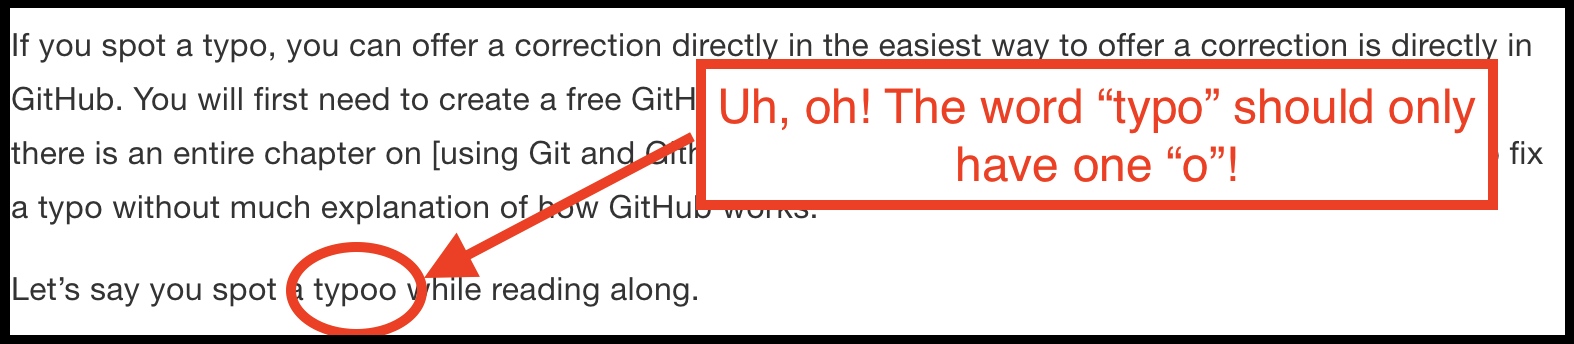
\includegraphics[keepaspectratio]{chapters/contributing/typo_on_screen.png}}

Next, click the edit button in the toolbar as shown in the screenshot
below.

\pandocbounded{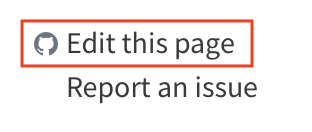
\includegraphics[keepaspectratio]{chapters/contributing/edit_button.png}}

The first time you click the icon, you will be taken to the R4Epi
repository on GitHub and asked to fork it. For our purposes, you can
think of a GitHub repository as being similar to a shared folder on
Dropbox or Google Drive.

\pandocbounded{
\includegraphics[keepaspectratio]{chapters/contributing/fork_button.png}}

``Forking the repository'' basically just means ``make a copy of the
repository'' on your GitHub account. In other words, copy all of the
files that make up the R4Epi textbook to your GitHub account. Then, you
can fix the typos you found in your \emph{copy} of the files that make
up the book instead of directly editing the \emph{actual} files that
make up the book. This is a safeguard to prevent people from
accidentally making changes that shouldn't be made.

\begin{tcolorbox}[enhanced jigsaw, toptitle=1mm, breakable, colback=white, toprule=.15mm, leftrule=.75mm, arc=.35mm, opacityback=0, coltitle=black, left=2mm, bottomrule=.15mm, bottomtitle=1mm, opacitybacktitle=0.6, title=\textcolor{quarto-callout-note-color}{\faInfo}\hspace{0.5em}{Note}, colframe=quarto-callout-note-color-frame, titlerule=0mm, rightrule=.15mm, colbacktitle=quarto-callout-note-color!10!white]

Forking the R4Epi repository does not cost any money or add any files to
your computer.

\end{tcolorbox}

After you fork the repository, you will see a text editor on your
screen.

\pandocbounded{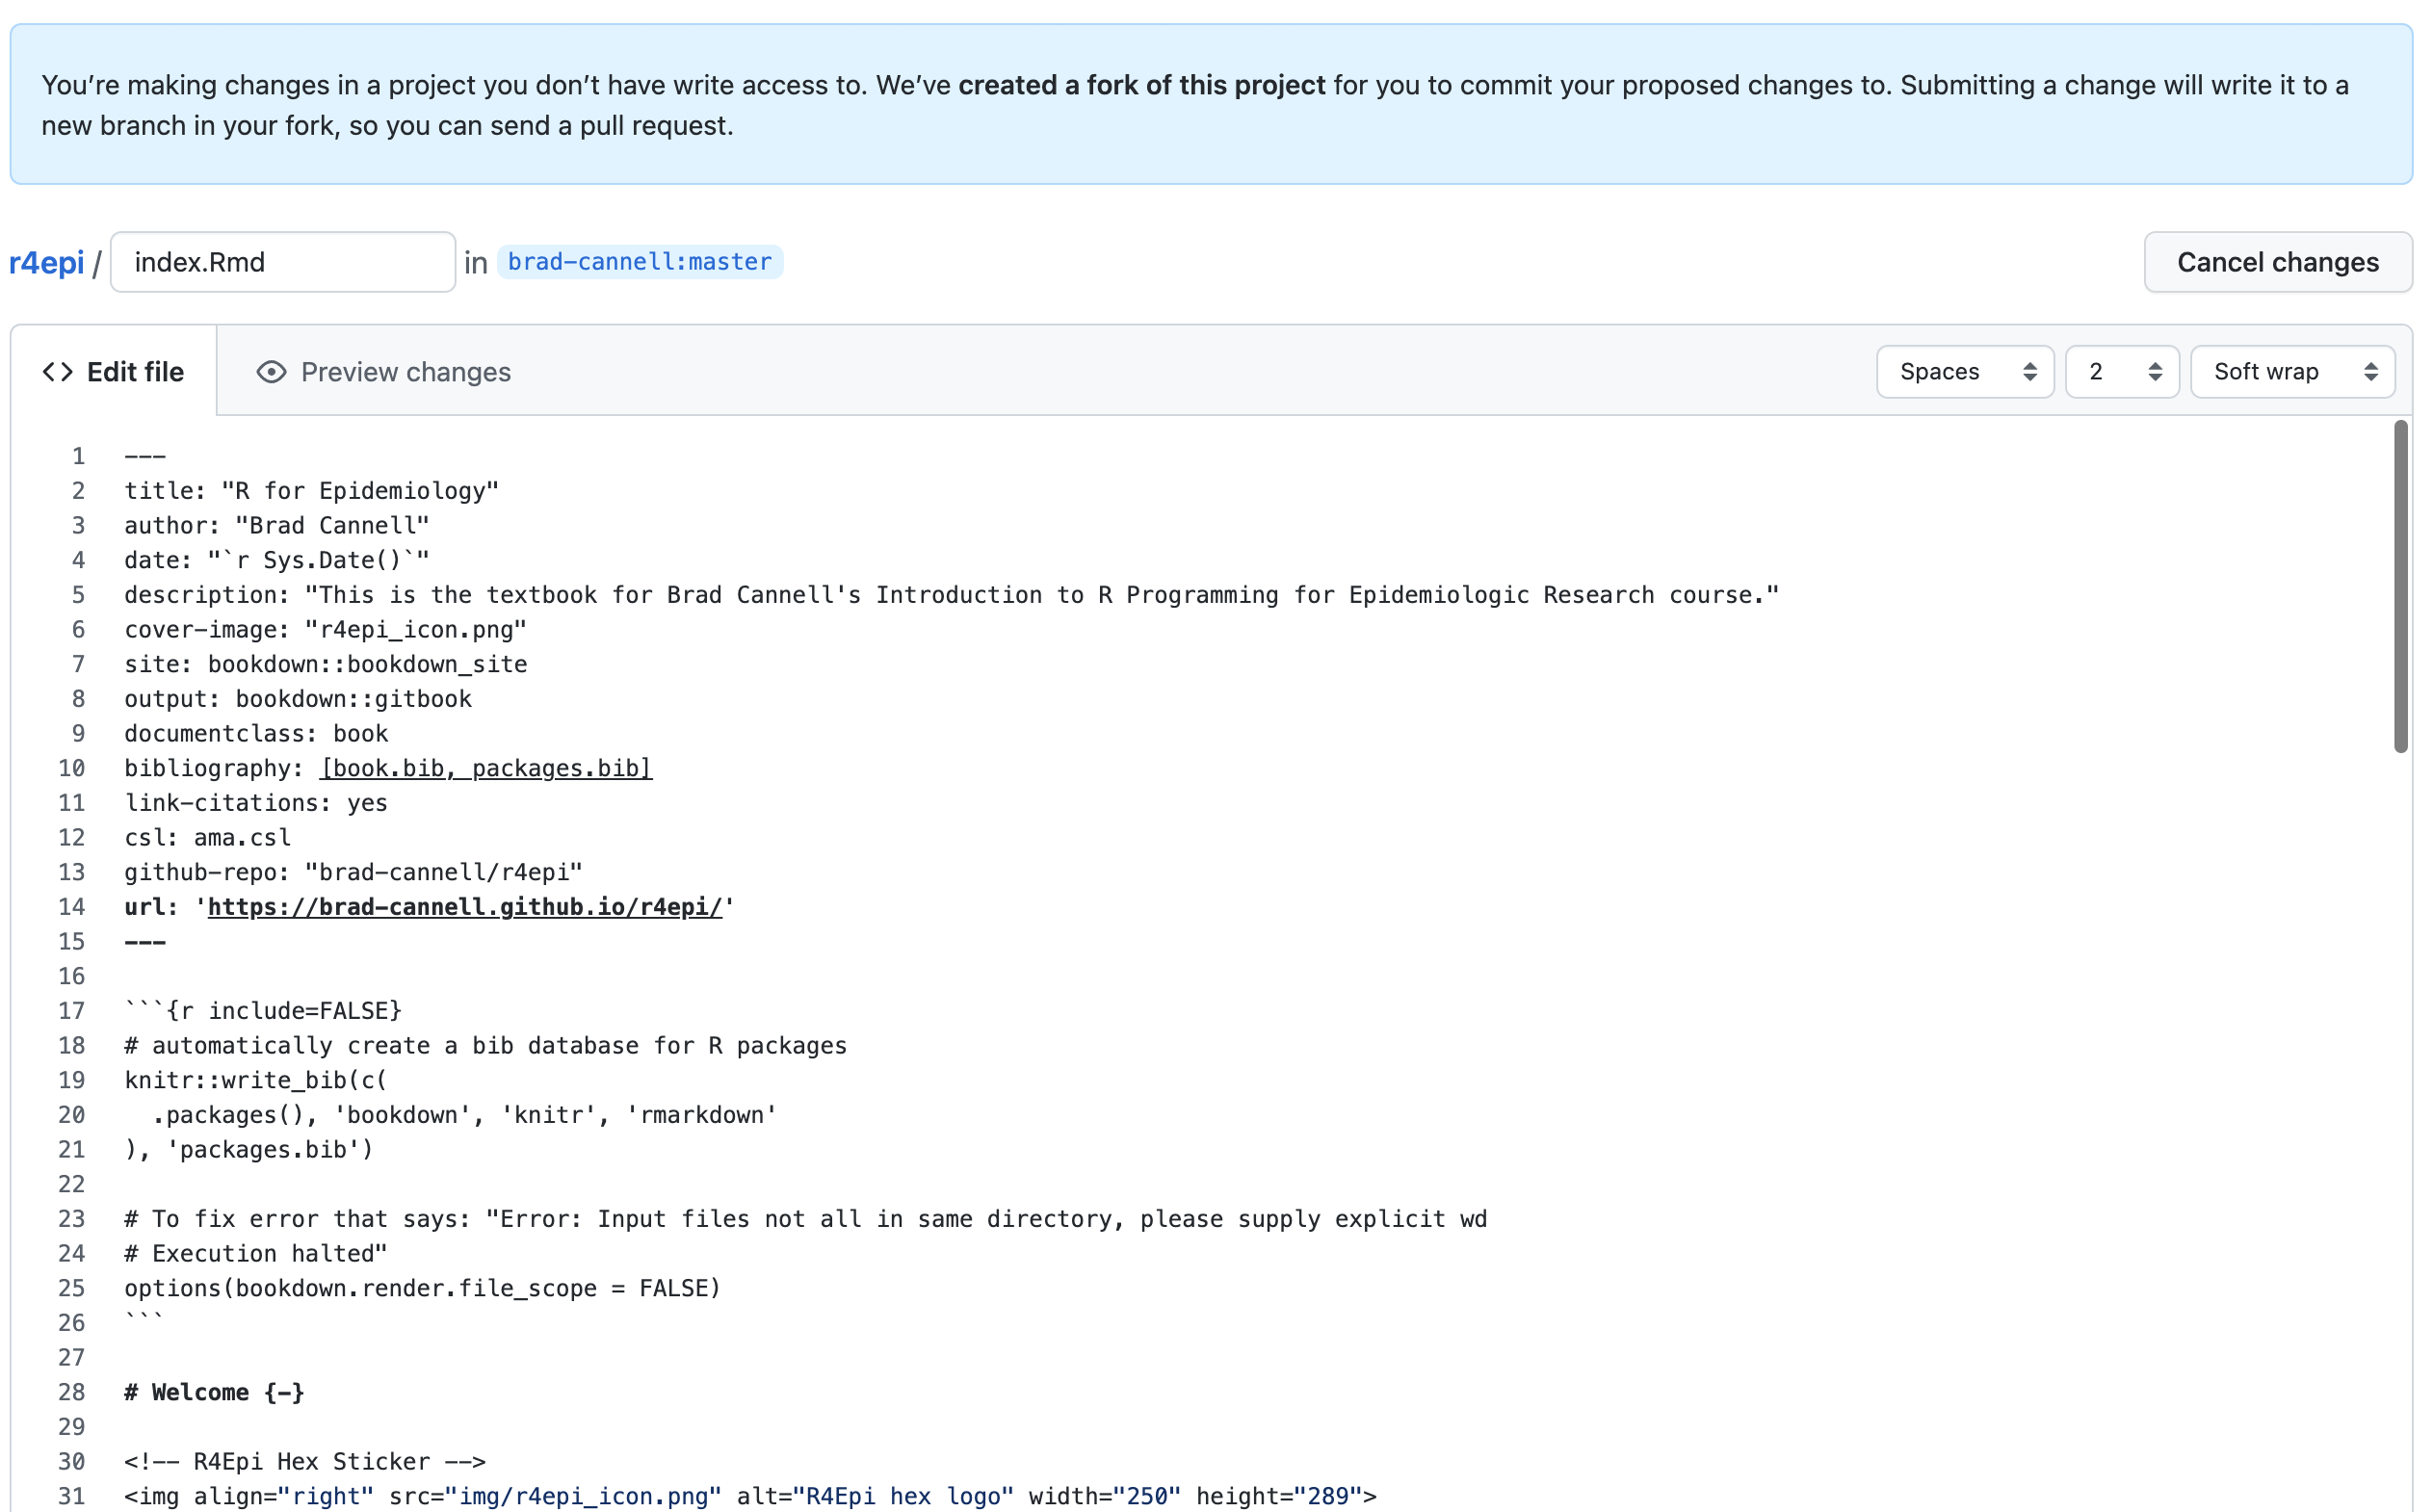
\includegraphics[keepaspectratio]{chapters/contributing/text_editor.png}}

The text editor will display the contents of the file used to make the
chapter you were looking at when you clicked the \texttt{edit} button.
In this example, it was a file named \texttt{contributing.qmd}. The
\texttt{.qmd} file extension means that the file is a Quarto/file. We
will learn more about \href{../quarto_files/quarto_files.qmd}{Quarto
files}, but for now just know that Quarto/ files can be used to create
web pages and other documents that contain a mix of R code, text, and
images.

Next, scroll down through the text until you find the typo and fix it.
In this case, line 11 contains the word ``typoo''. To fix it, you just
need to click in the editor window and begin typing. In this case, you
would click next to the word ``typoo'' and delete the second ``o''.

\pandocbounded{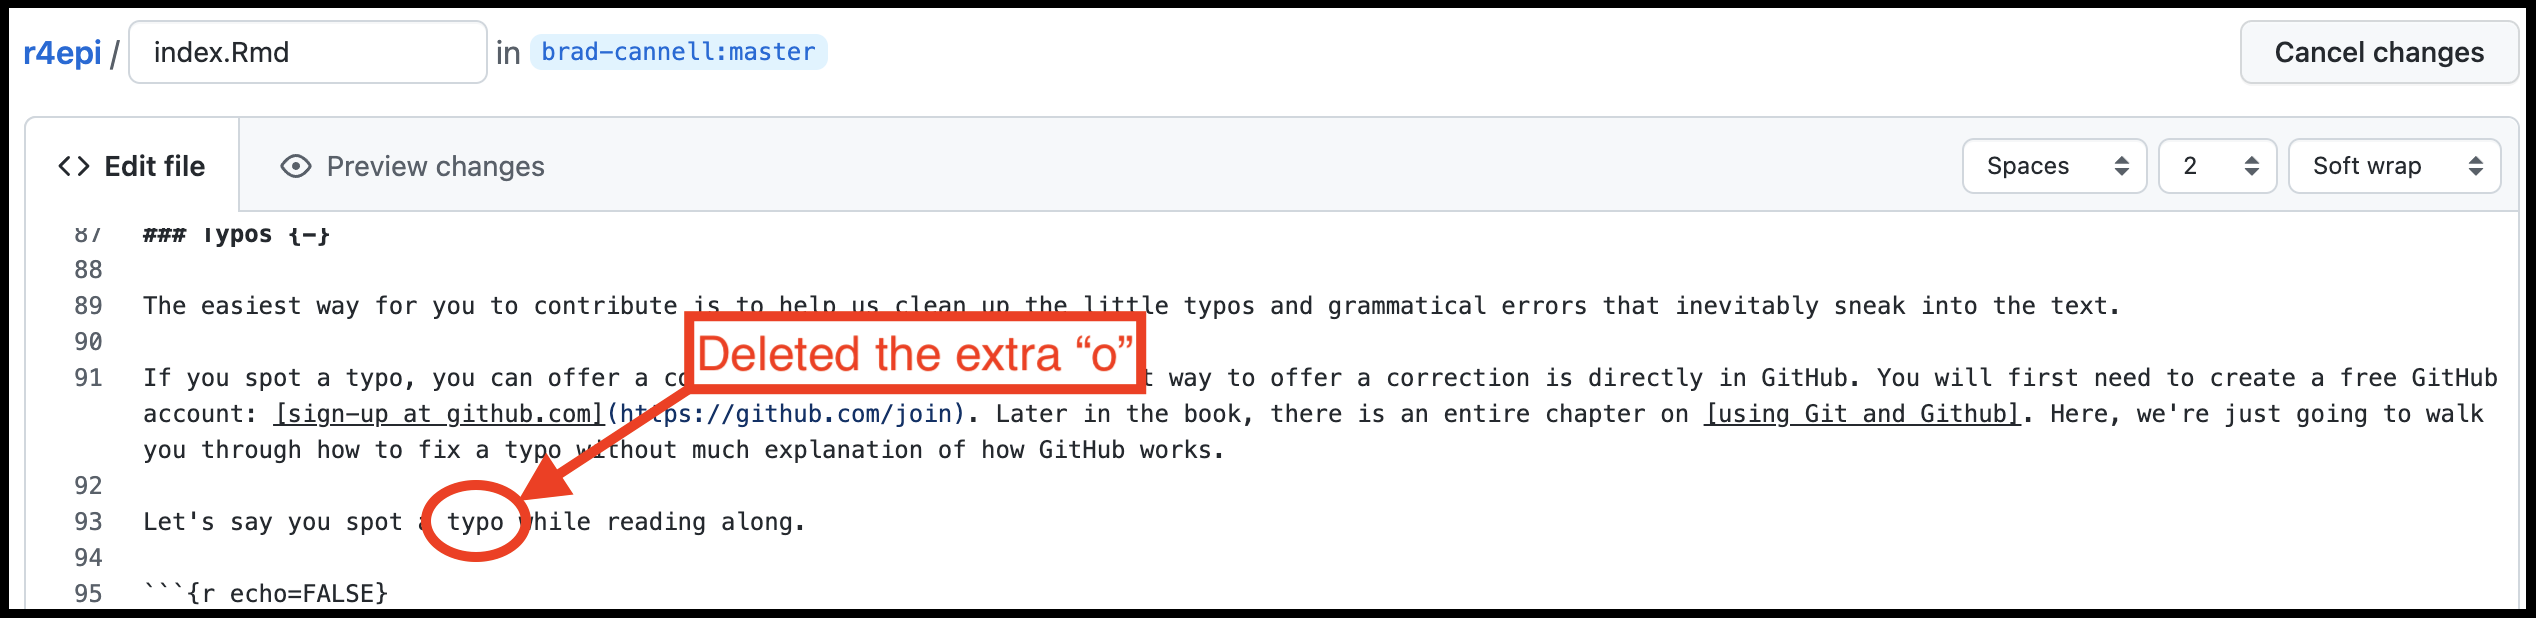
\includegraphics[keepaspectratio]{chapters/contributing/fix_typo.png}}

Now, the only thing left to do is propose your typo fix to the authors.
To do so, click the green \texttt{Commit\ changes...} button on the
right side of the screen above the text editor (surrounded with a red
box in the screenshot above). When you click it, a new
\texttt{Propose\ changes} box will appear on your screen. Type a brief
(i.e., 72 characters or less) summary of the change you made in the
\texttt{Commit\ message} box. There is also an
\texttt{Extended\ description} box where you can add a more detailed
description of what you did. In the screenshot below, shows an example
commit message and extended description that will make it easy for the
author to quickly figure out exactly what changes are being proposed.

\pandocbounded{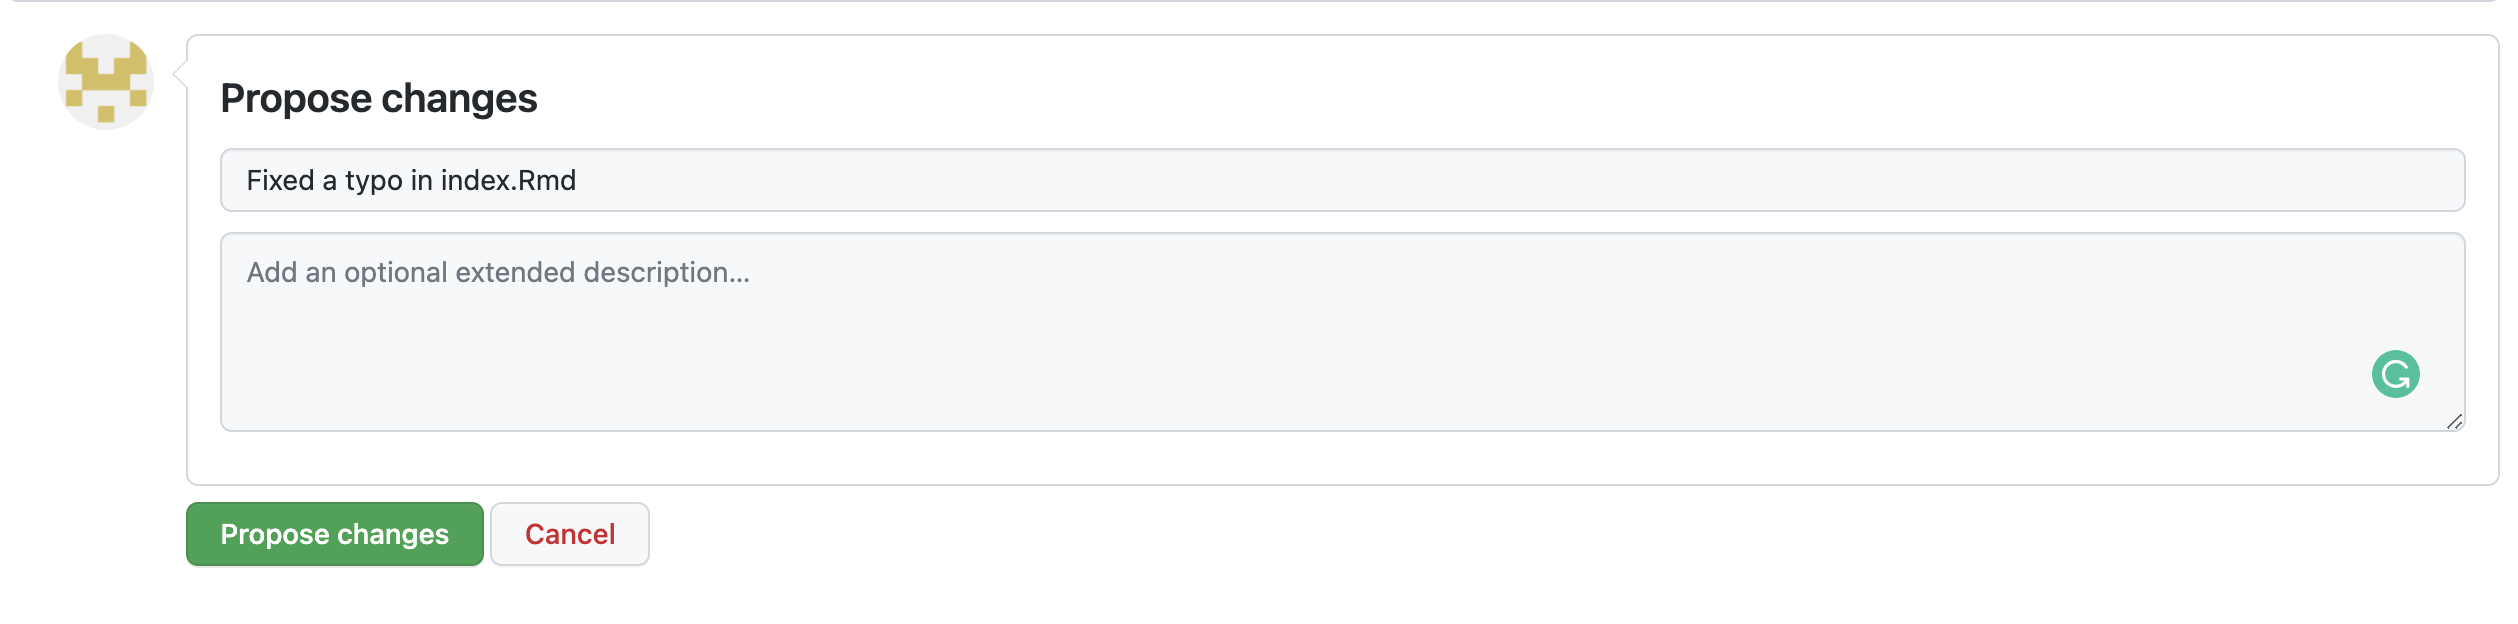
\includegraphics[keepaspectratio]{chapters/contributing/propose_changes.png}}

Next, click the \texttt{Propose\ changes} button. That will take you to
another screen where you will be able to create a pull request. This
screen is kind of busy, but try not to let it overwhelm you.

\pandocbounded{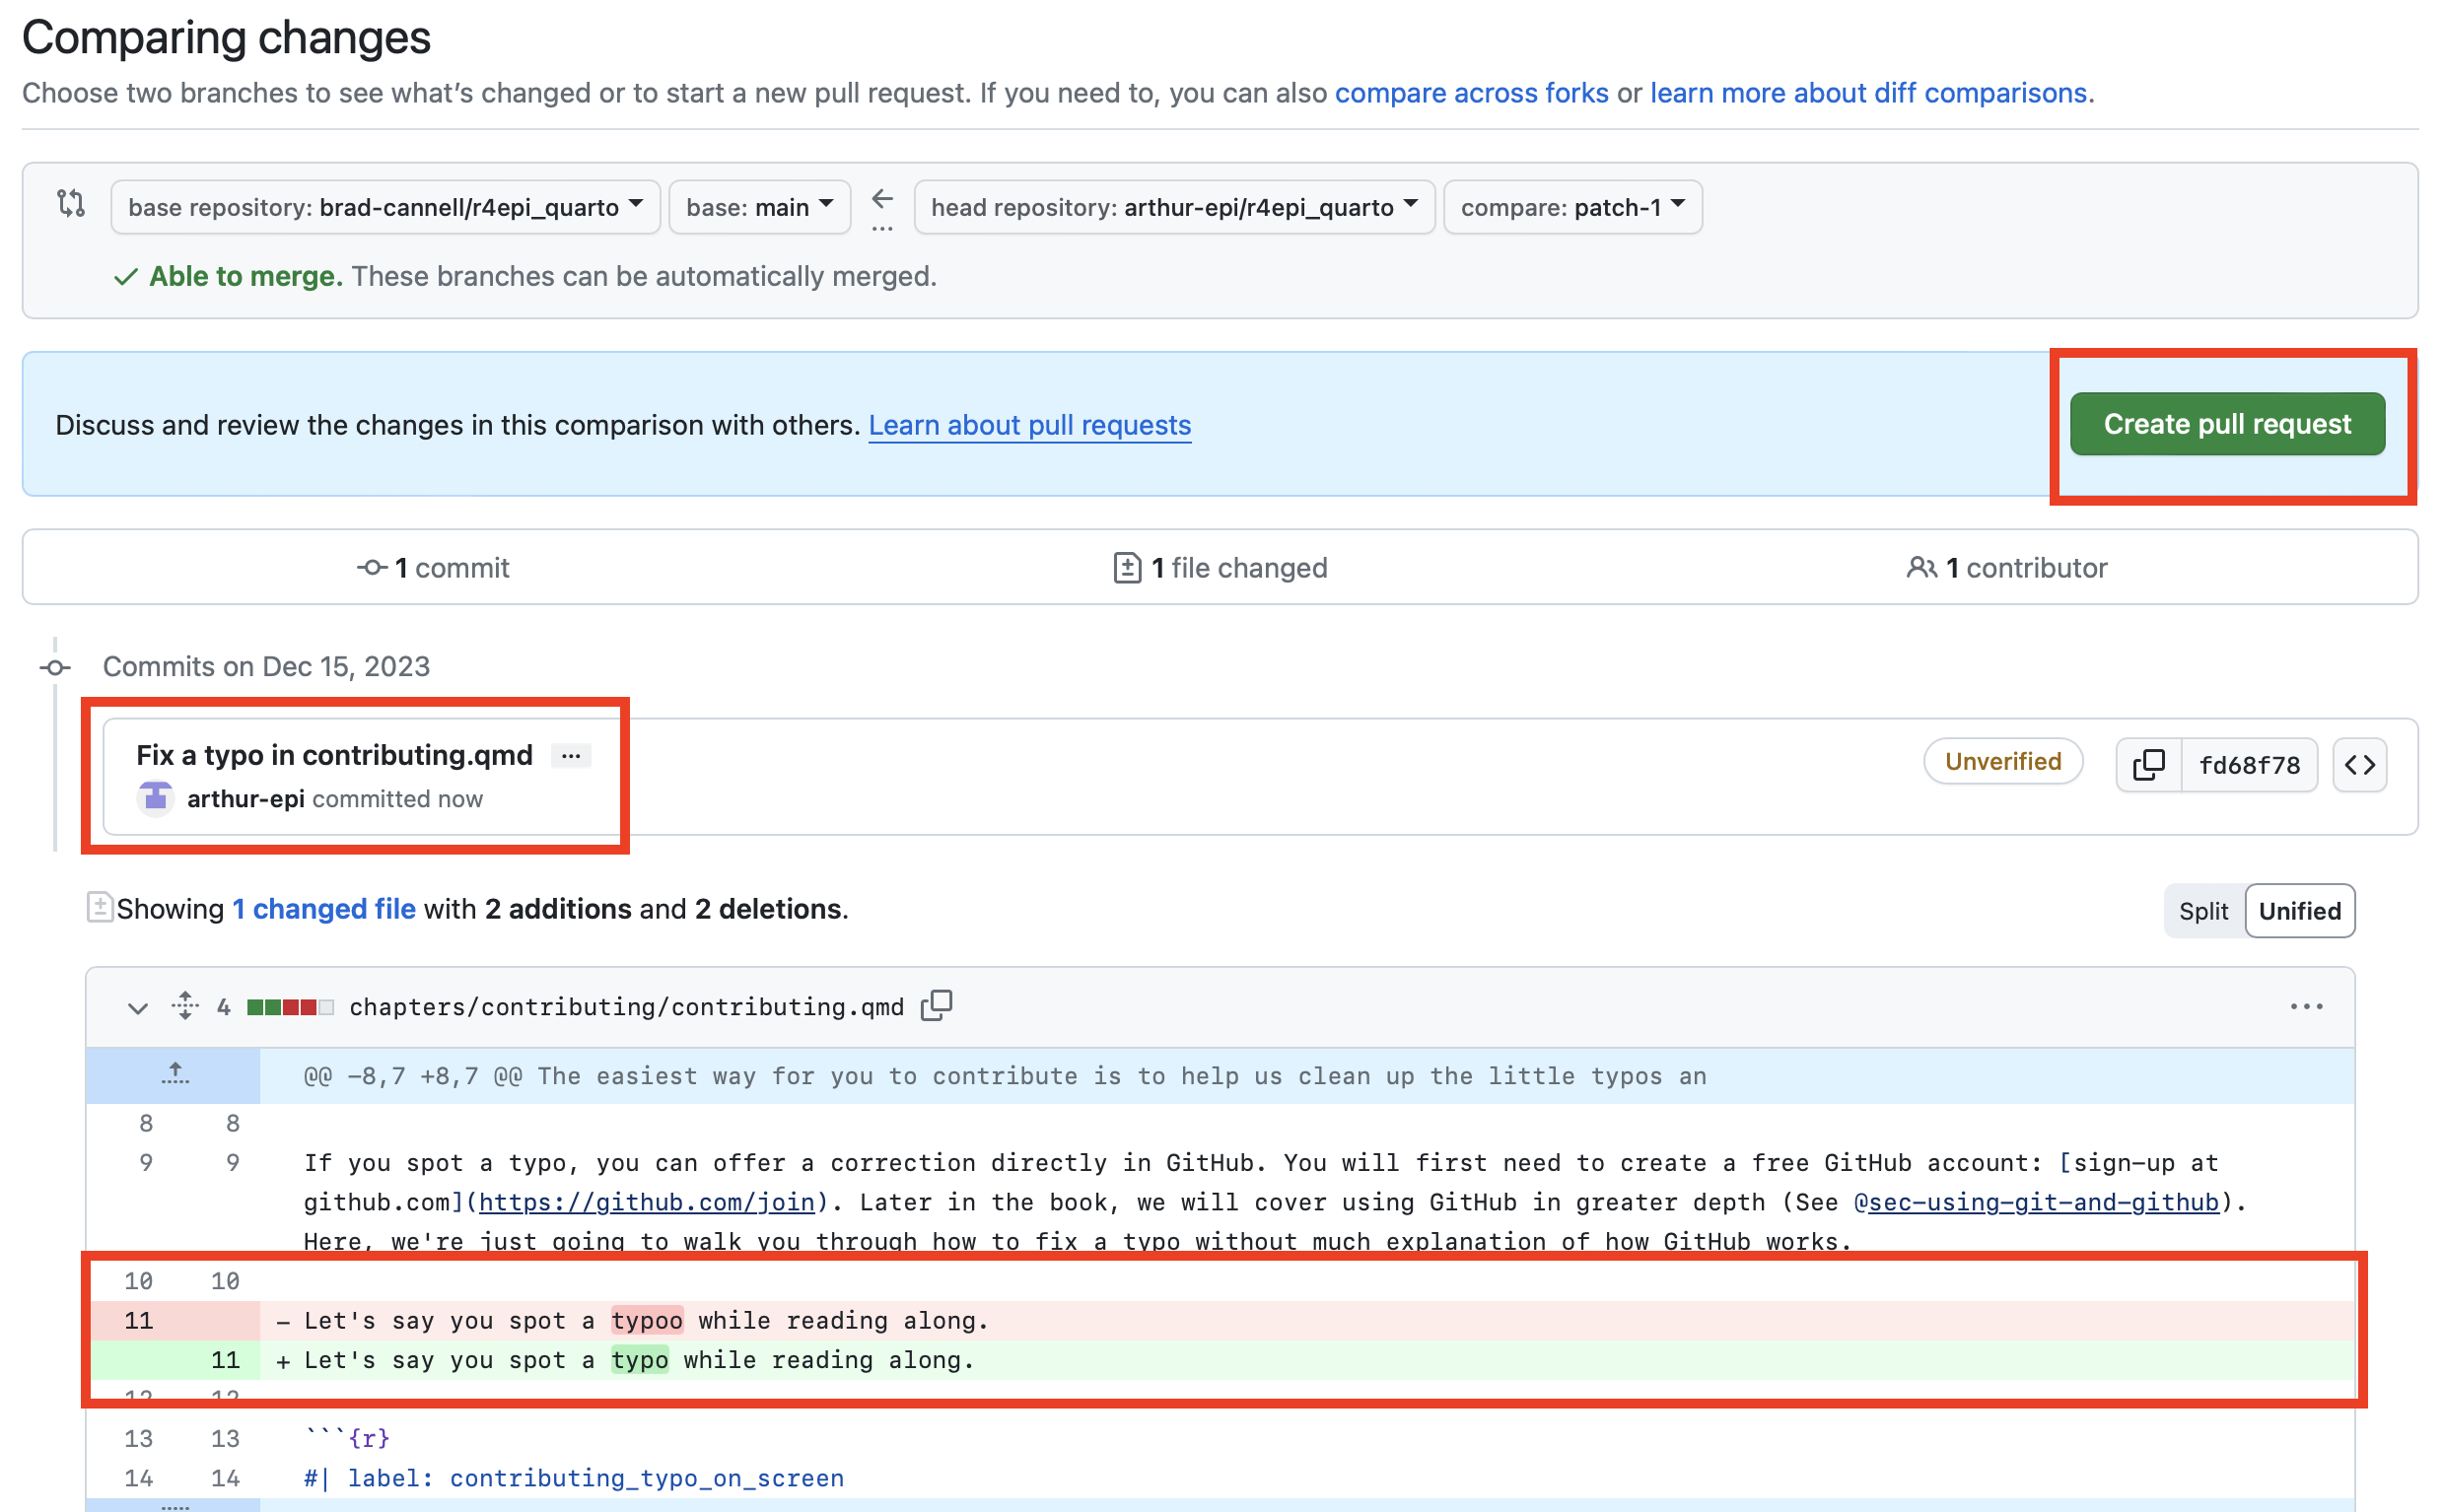
\includegraphics[keepaspectratio]{chapters/contributing/create_pull_request_1.png}}

For now, we will focus on the three different sections of the screen
that are highlighted with a red outline. We will start at the bottom and
work our way up. The red box that is closest to the bottom of the
screenshot shows us that the change that made was on line 11. The word
``typoo'' (highlighted in red) was replaced with the word ``typo''
(highlighted in green). The red box in the middle of the screenshot
shows us the brief description that was written for our proposed change
-- ``Fix a typo in contributing.qmd''. Finally, the red box closest to
the top of the screenshot is surrounding the
\texttt{Create\ pull\ request} button. You will click it to move on with
your pull request.

\pandocbounded{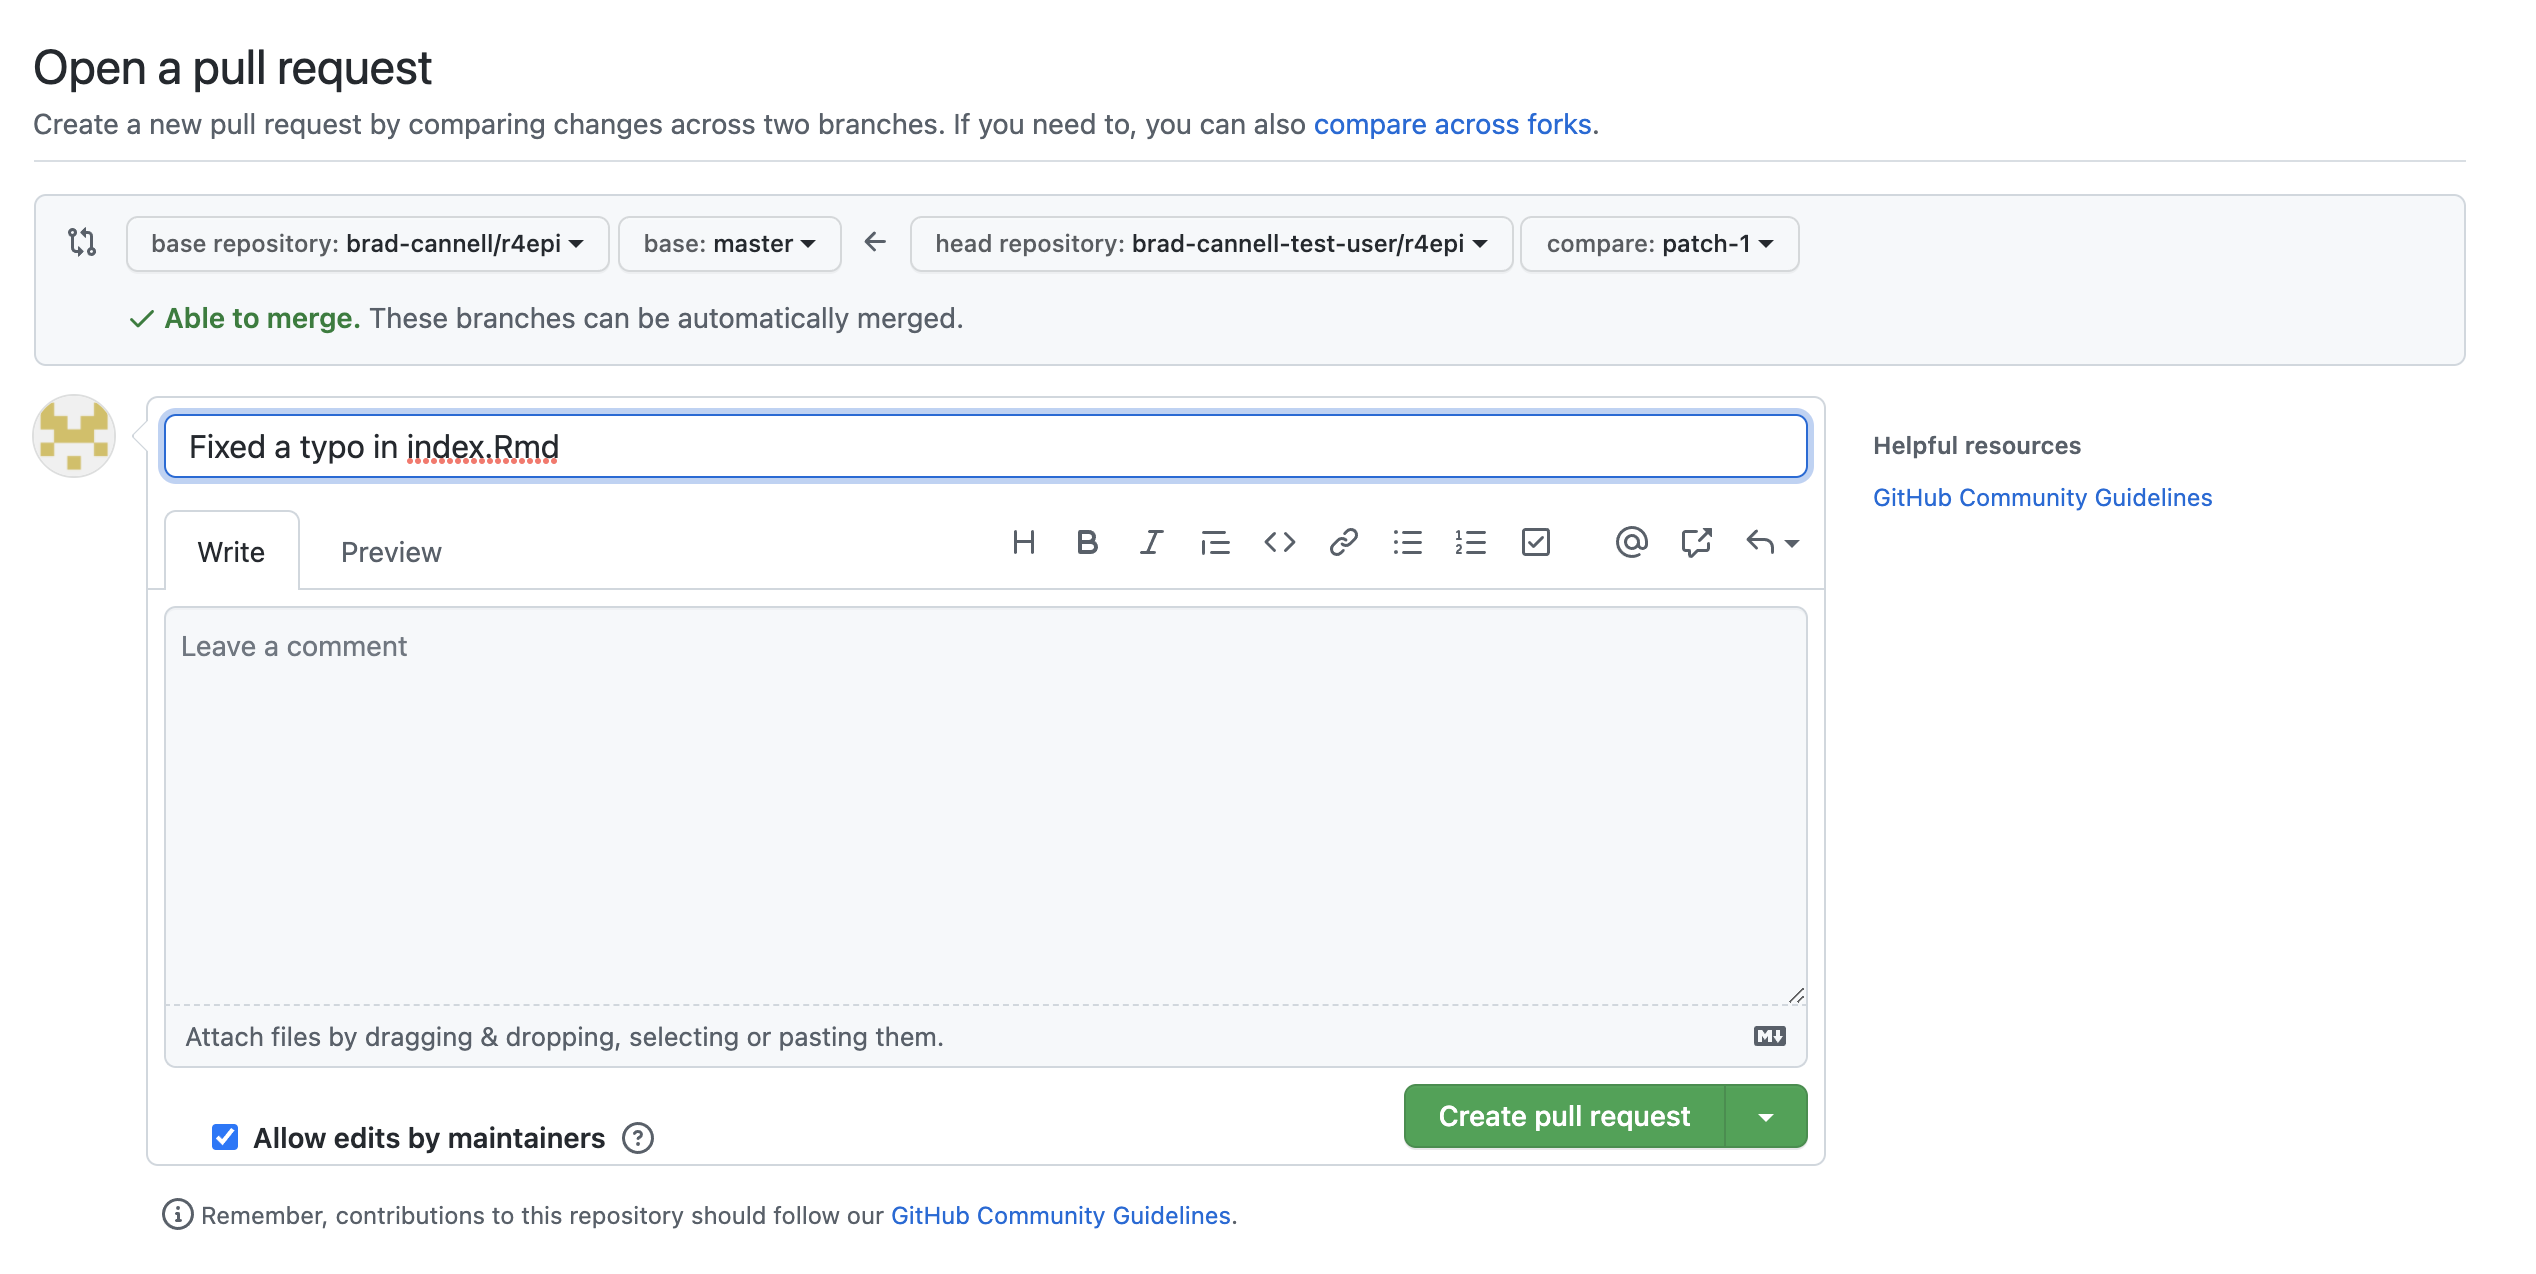
\includegraphics[keepaspectratio]{chapters/contributing/create_pull_request_2.png}}

After doing so, you will get one final chance to amend the description
of your proposed changes. If you are happy with the commit message and
description, then click the \texttt{Create\ pull\ request} button one
more time. At this point, your job is done! It is now up to the authors
to review the changes you've proposed and ``pull'' them into the file in
their repository.

In case you are curious, here is what the process looks like on the
authors' end. First, when we open the R4Epi repository page on GitHub,
we will see that there is a new pull request.

\pandocbounded{
\includegraphics[keepaspectratio]{chapters/contributing/create_pull_request_3.png}}

When we open the pull request, we can see the proposed changes to the
file.

\pandocbounded{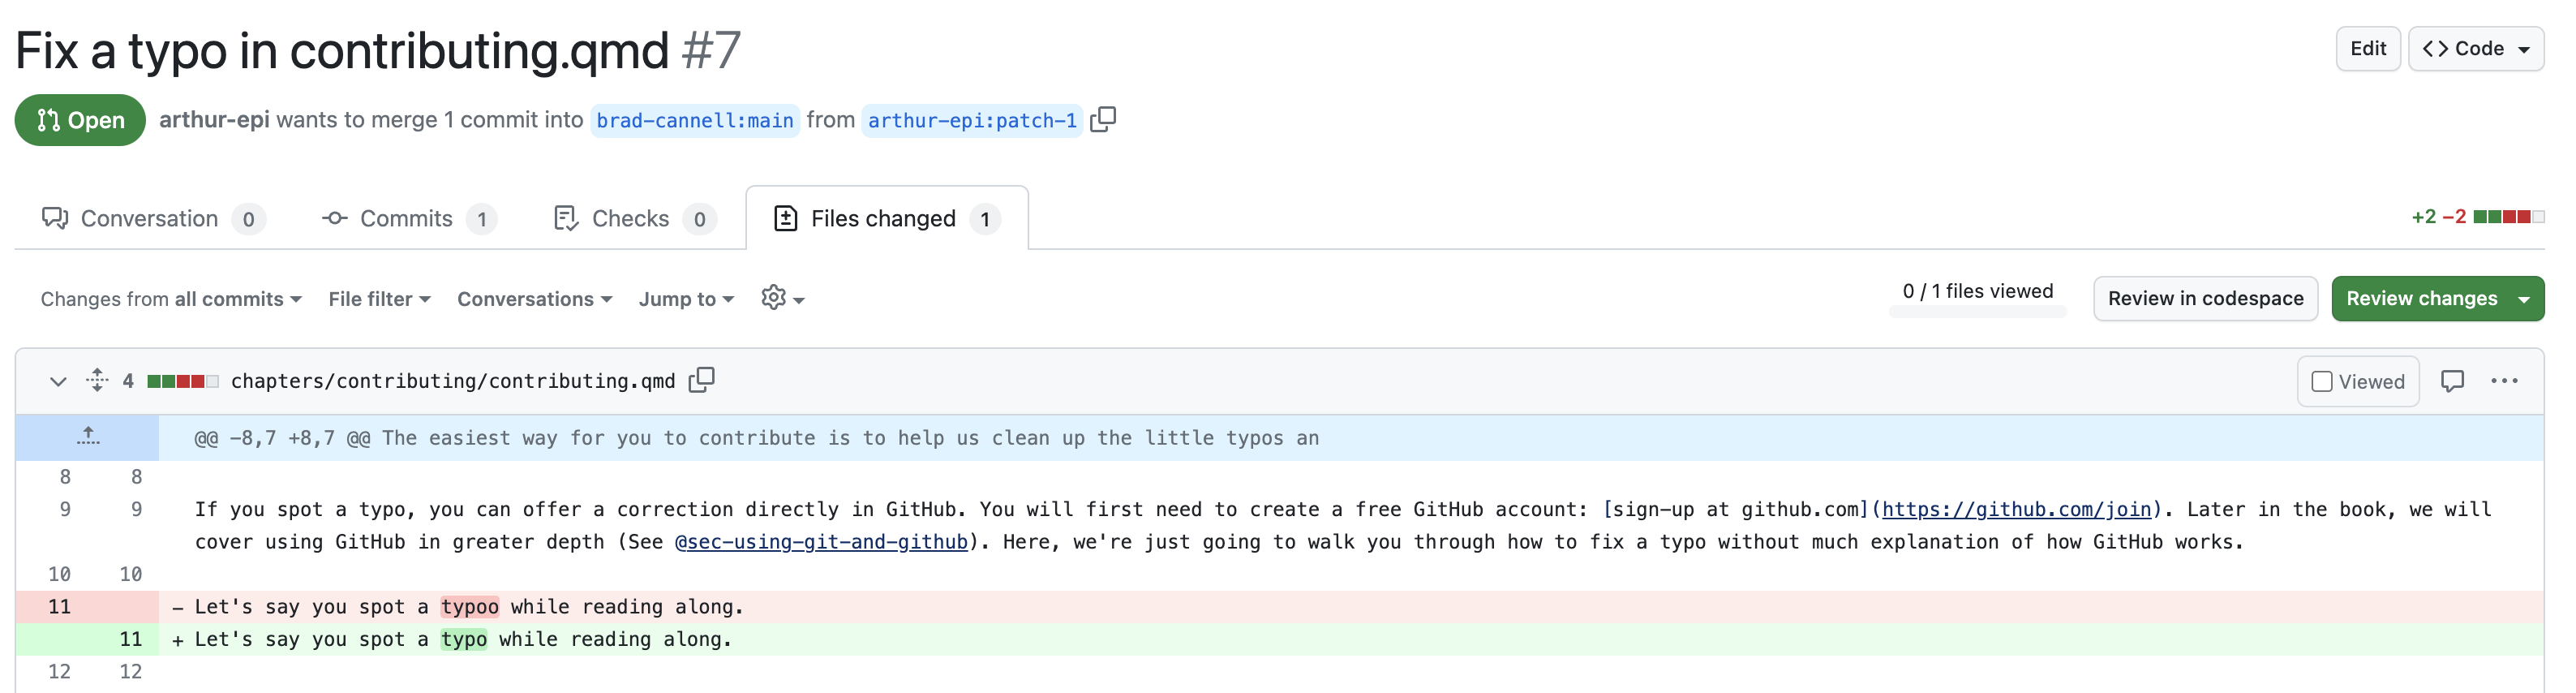
\includegraphics[keepaspectratio]{chapters/contributing/create_pull_request_4.png}}

Then, all we have to do is click the
\texttt{Merge\ pull\ request\ button} and the fixed file is ``pulled
in'' to replace the file with the typo.

\pandocbounded{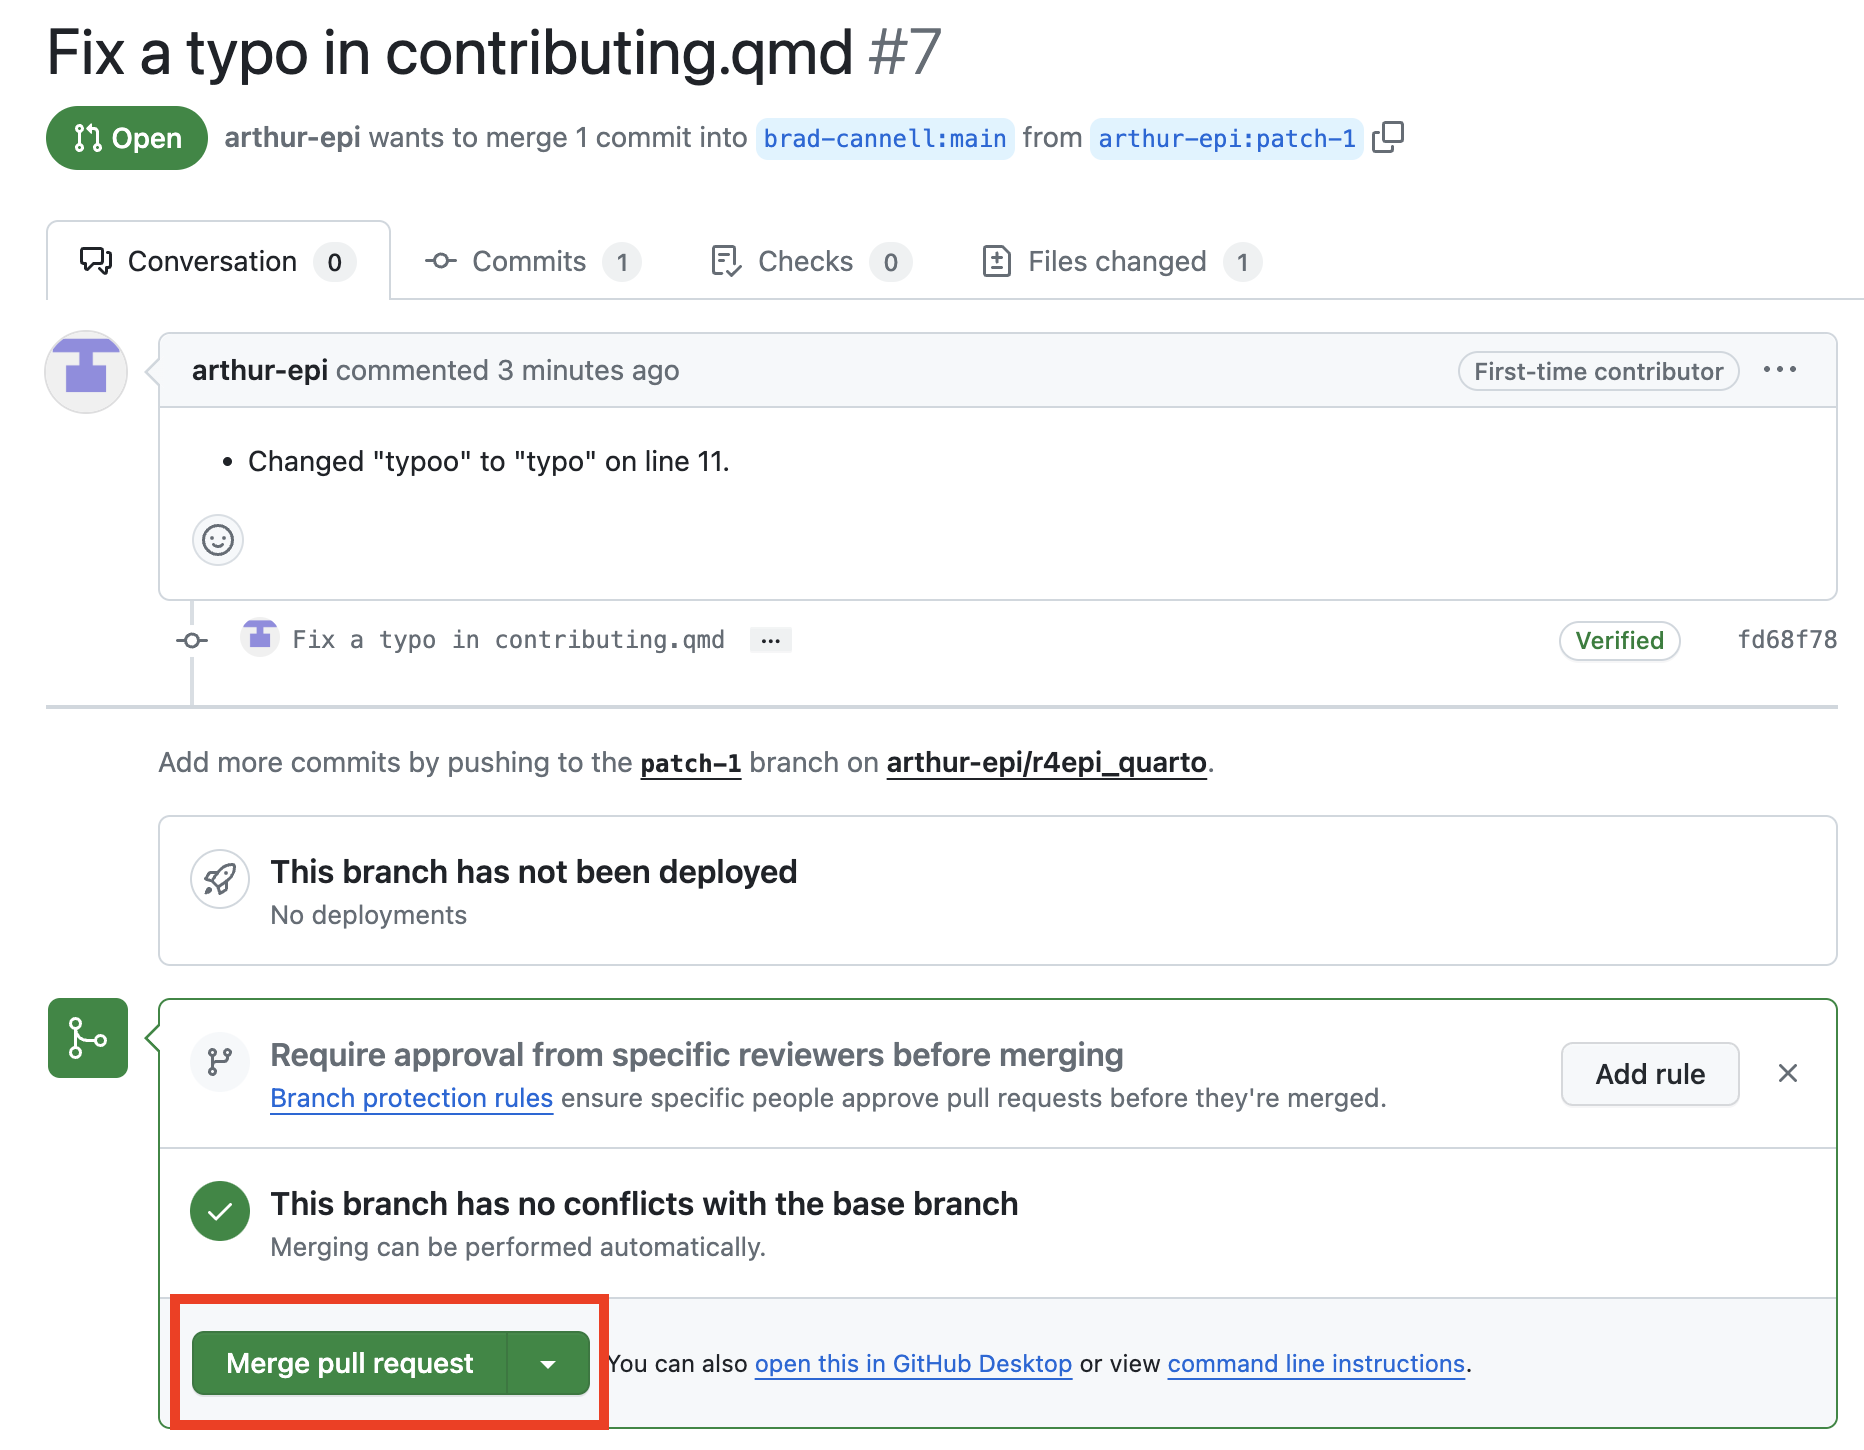
\includegraphics[keepaspectratio]{chapters/contributing/create_pull_request_5.png}}

\section*{Issues}\label{issues}
\addcontentsline{toc}{section}{Issues}

\markright{Issues}

There may be times when you see a problem that you don't know how to
fix, but you still want to make the authors aware of. In that case, you
can create an \hyperref[glossary-issue]{issue} in the R4Epi repository.
To do so, navigate to the issue tracker using this link:
\url{https://github.com/brad-cannell/r4epi/issues}.

\pandocbounded{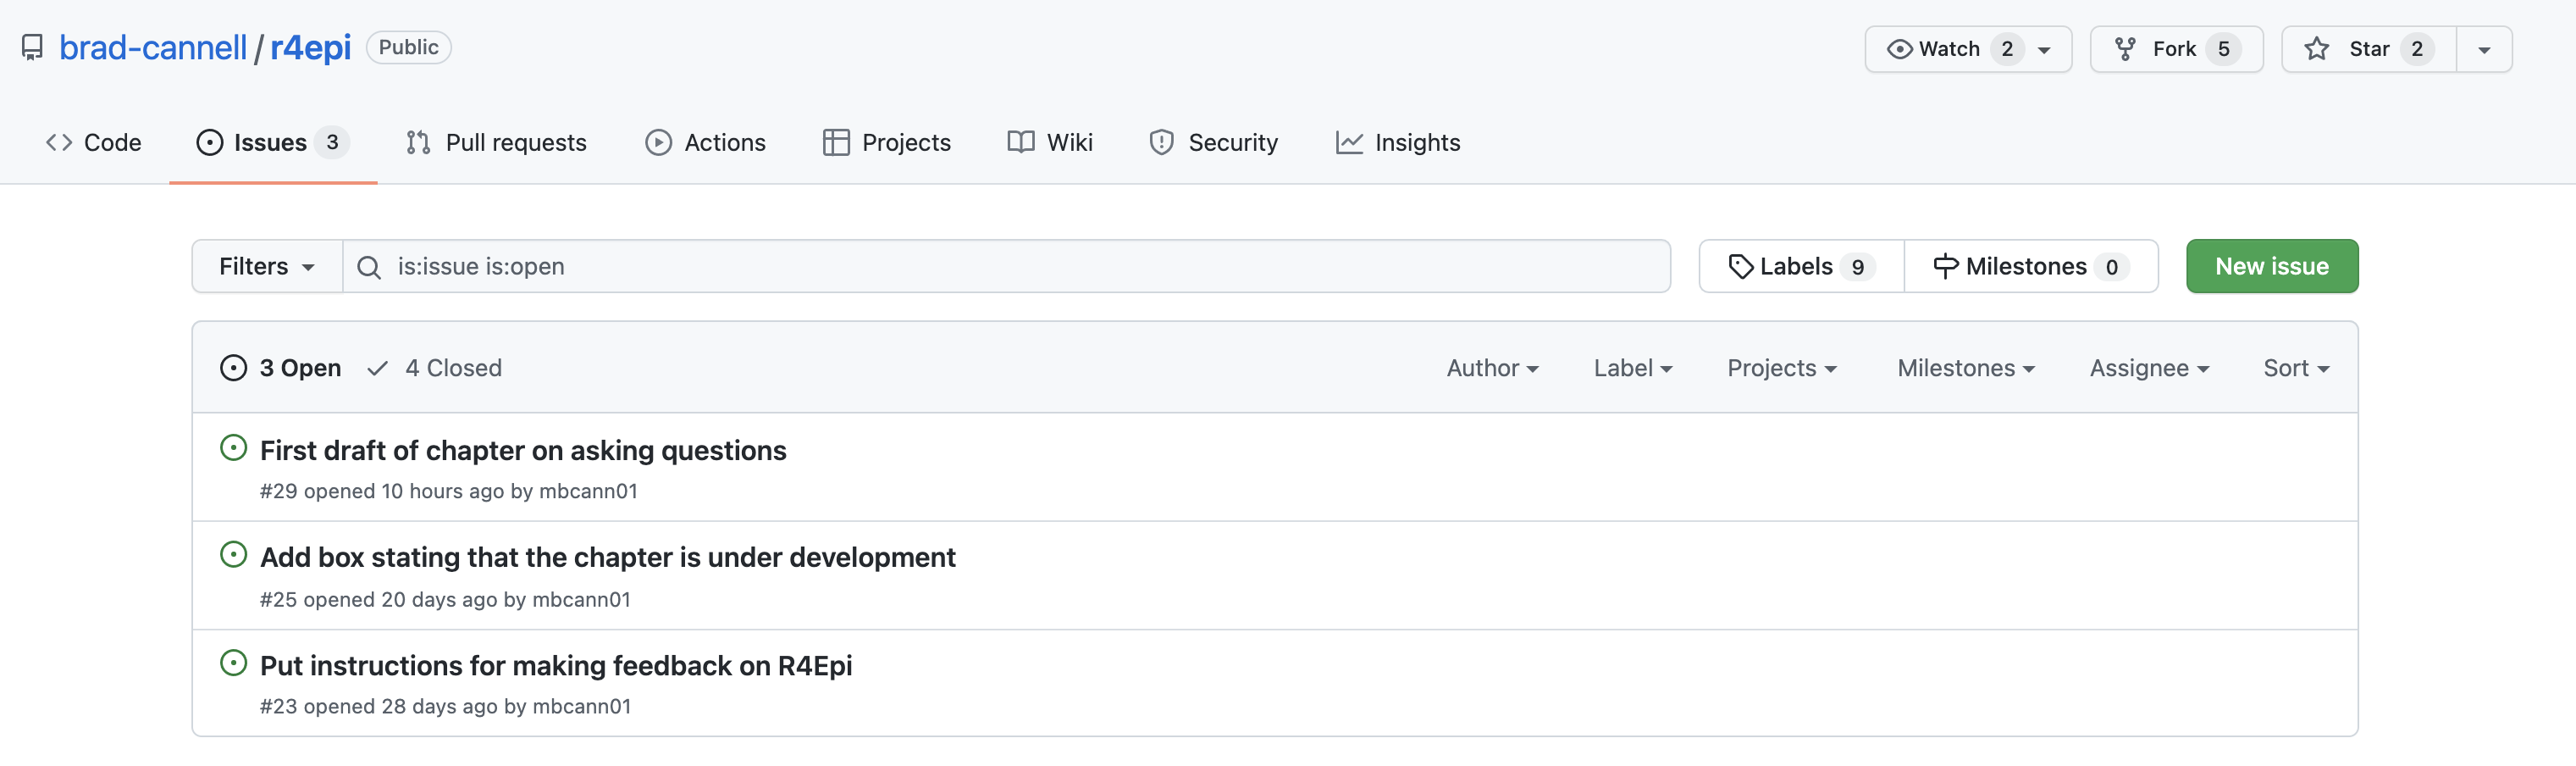
\includegraphics[keepaspectratio]{chapters/contributing/issue_tracker.png}}

Once there, you can check to see if someone has already raised the issue
you are concerned about. If not, you can click the green ``New issue''
button to raise it yourself.

Please note that R4Epi uses a
\href{https://contributor-covenant.org/version/2/0/CODE_OF_CONDUCT.html}{Contributor
Code of Conduct}. By contributing to this book, you agree to abide by
its terms.

\section*{License Information}\label{license-information}
\addcontentsline{toc}{section}{License Information}

\markright{License Information}

This book was created by Brad Cannell and is licensed under a Creative
Commons Attribution-NonCommercial-NoDerivatives 4.0 International
License.

\bookmarksetup{startatroot}

\chapter*{About the Authors}\label{about-the-authors}
\addcontentsline{toc}{chapter}{About the Authors}

\markboth{About the Authors}{About the Authors}

\section*{Brad Cannell}\label{brad-cannell}
\addcontentsline{toc}{section}{Brad Cannell}

\markright{Brad Cannell}

\textbf{Michael (Brad) Cannell, PhD, MPH}\\
Associate Professor\\
Elder Mistreatment Lead, UTHealth Institute of Aging\\
Director, Research Informatics Core, Cizik Nursing Research Institute\\
UTHealth Houston\\
McGovern Medical School\\
Joan and Stanford Alexander Division of Geriatric \& Palliative
Medicine\\
\href{https://www.bradcannell.com}{www.bradcannell.com}

Dr.~Cannell received his PhD in Epidemiology, and Graduate Certificate
in Gerontology, in 2013 from the University of Florida. He received his
MPH with a concentration in Epidemiology from the University of
Louisville in 2009, and his BA in Political Science and Marketing from
the University of North Texas in 2005. During his doctoral studies, he
was a Graduate Research Assistant for the Florida Office on Disability
and Health, an affiliated scholar with the Claude D. Pepper Older
Americans Independence Center, and a student-inducted member of the
Delta Omega Honorary Society in Public Health. In 2016, Dr.~Cannell
received a Graduate Certificate in Predictive Analytics from the
University of Maryland University College, and a Certificate in Big Data
and Social Analytics from the Massachusetts Institute of Technology.

He previously held professional staff positions in the Louisville Metro
Health Department and the Northern Kentucky Independent District Health
Department. He spent three years as a project epidemiologist for the
Florida Office on Disability and Health at the University of Florida. He
also served as an Environmental Science Officer in the United States
Army Reserves from 2009 to 2013.

Dr.~Cannell's research is broadly focused on healthy aging and
health-related quality of life. Specifically, he has published research
focusing on preservation of physical and cognitive function, living and
aging with disability, and understanding and preventing elder
mistreatment. Additionally, he has a strong background and training in
epidemiologic methods and predictive analytics. He has been principal or
co-investigator on multiple trials and observational studies in
community and healthcare settings. He is currently the principal
investigator on multiple data-driven federally funded projects that
utilize technological solutions to public health issues in novel ways.

\textbf{Contact}\\
Connect with Dr.~Cannell and follow his work.\\

\includegraphics[width=2em,height=2em]{chapters/about_the_authors/about_the_authors_files/figure-pdf/fa-icon-a4a233699ebb8edeaca4e7ae0455099b.pdf}

\includegraphics[width=1.75em,height=2em]{chapters/about_the_authors/about_the_authors_files/figure-pdf/fa-icon-d19241927d9e636802f0f0caca52c0af.pdf}

\includegraphics[width=1.75em,height=2em]{chapters/about_the_authors/about_the_authors_files/figure-pdf/fa-icon-f2455331e499245af38ff1988a0023d4.pdf}

\includegraphics[width=1.75em,height=2em]{chapters/about_the_authors/about_the_authors_files/figure-pdf/fa-icon-1cbfc0b82b7e84c9b17b238bfd9a886e.pdf}

\section*{Melvin Livingston}\label{melvin-livingston}
\addcontentsline{toc}{section}{Melvin Livingston}

\markright{Melvin Livingston}

\textbf{Melvin (Doug) Livingston, PhD}\\
Research Associate Professor\\
Department of Behavioral, Social, and Health Education Sciences\\
Emory University Woodruff Health Sciences Center\\
Rollins School of Public Health\\
\href{https://sph.emory.edu/faculty/profile/index.php?FID=melvin-livingston-8970}{Dr.~Livingston's
Faculty Profile}

Dr.~Livingston is a methodologist with expertise in the the application
of quasi-experimental design principals to the evaluation for both
community interventions and state policies. He has particular expertise
in time series modeling, mixed effects modeling, econometric methods,
and power analysis. As part of his work involving community trials, he
has been the statistician on the long term follow-up study of a school
based cluster randomized trial in low-income communities with a focus on
explaining the etiology of risky alcohol, drug, and sexual behaviors.
Additionally, he was the statistician for a longitudinal study examining
the etiology of alcohol use among racially diverse and economically
disadvantaged urban youth, and co-investigator for a NIAAA- and
NIDA-funded trial to prevent alcohol use and alcohol-related problems
among youth living in high-risk, low-income communities within the
Cherokee Nation. Prevention work at the community level led him to an
interest in the impact of state and federal socioeconomic policies on
health outcomes. He is a Co-Investigator of a 50-state, 30-year study of
effects of state-level economic and education policies on a diverse set
of public health outcomes, explicitly examining differential effects
across disadvantaged subgroups of the population.

His current research interests center around the application of
quasi-experimental design and econometric methods to the evaluation of
the health effects of state and federal policy.

\textbf{Contact}\\
Connect with Dr.~Livingston and follow his work.\\

\includegraphics[width=2em,height=2em]{chapters/about_the_authors/about_the_authors_files/figure-pdf/fa-icon-a4a233699ebb8edeaca4e7ae0455099b.pdf}

\includegraphics[width=1.75em,height=2em]{chapters/about_the_authors/about_the_authors_files/figure-pdf/fa-icon-ab37b36564b32e84e458655a90d49135.pdf}

\part{Getting Started}

\chapter{Installing R and RStudio}\label{installing-r-and-rstudio}

Before we can do any programming with \hyperref[glossary-r]{R}, we first
have to download it to our computer. Fortunately, R is free, easy to
install, and runs on all major operating systems (i.e., Mac and
Windows). However, R is even easier to use as when we combine it with
another program called \hyperref[glossary-rstudio]{RStudio}.
Fortunately, RStudio is also free and will also run on all major
operating systems.

At this point, you may be wondering what R is, what RStudio is, and how
they are related. We will answer those questions in the near future.
However, in the interest of keeping things brief and simple, We're not
going to get into them right now. Instead, all you have to worry about
is getting the R programming language and the RStudio IDE (IDE is short
for integrated development environment) downloaded and installed on your
computer. The steps involved are slightly different depending on whether
you are using a Mac or a PC (i.e., Windows). Therefore, please feel free
to use the table of contents on the right-hand side of the screen to
navigate directly to the instructions that you need for your computer.

\begin{tcolorbox}[enhanced jigsaw, toptitle=1mm, breakable, colback=white, toprule=.15mm, leftrule=.75mm, arc=.35mm, opacityback=0, coltitle=black, left=2mm, bottomrule=.15mm, bottomtitle=1mm, opacitybacktitle=0.6, title=\textcolor{quarto-callout-note-color}{\faInfo}\hspace{0.5em}{Note}, colframe=quarto-callout-note-color-frame, titlerule=0mm, rightrule=.15mm, colbacktitle=quarto-callout-note-color!10!white]

In this chapter, we cover how to download and install R and RStudio on
both Mac and PC. However, the screenshots in all following chapters will
be from a Mac. The good news is that RStudio operates almost identically
on Mac and PC.

\end{tcolorbox}

\textbf{Step 1:} Regardless of which operating system you are using,
please make sure your computer is on, properly functioning, connected to
the internet, and has enough space on your hard drive to save R and
RStudio.

\section{Download and install on a
Mac}\label{download-and-install-on-a-mac}

\textbf{Step 2:} Navigate to the Comprehensive R Archive Network (CRAN),
which is located at https://cran.r-project.org/.

\pandocbounded{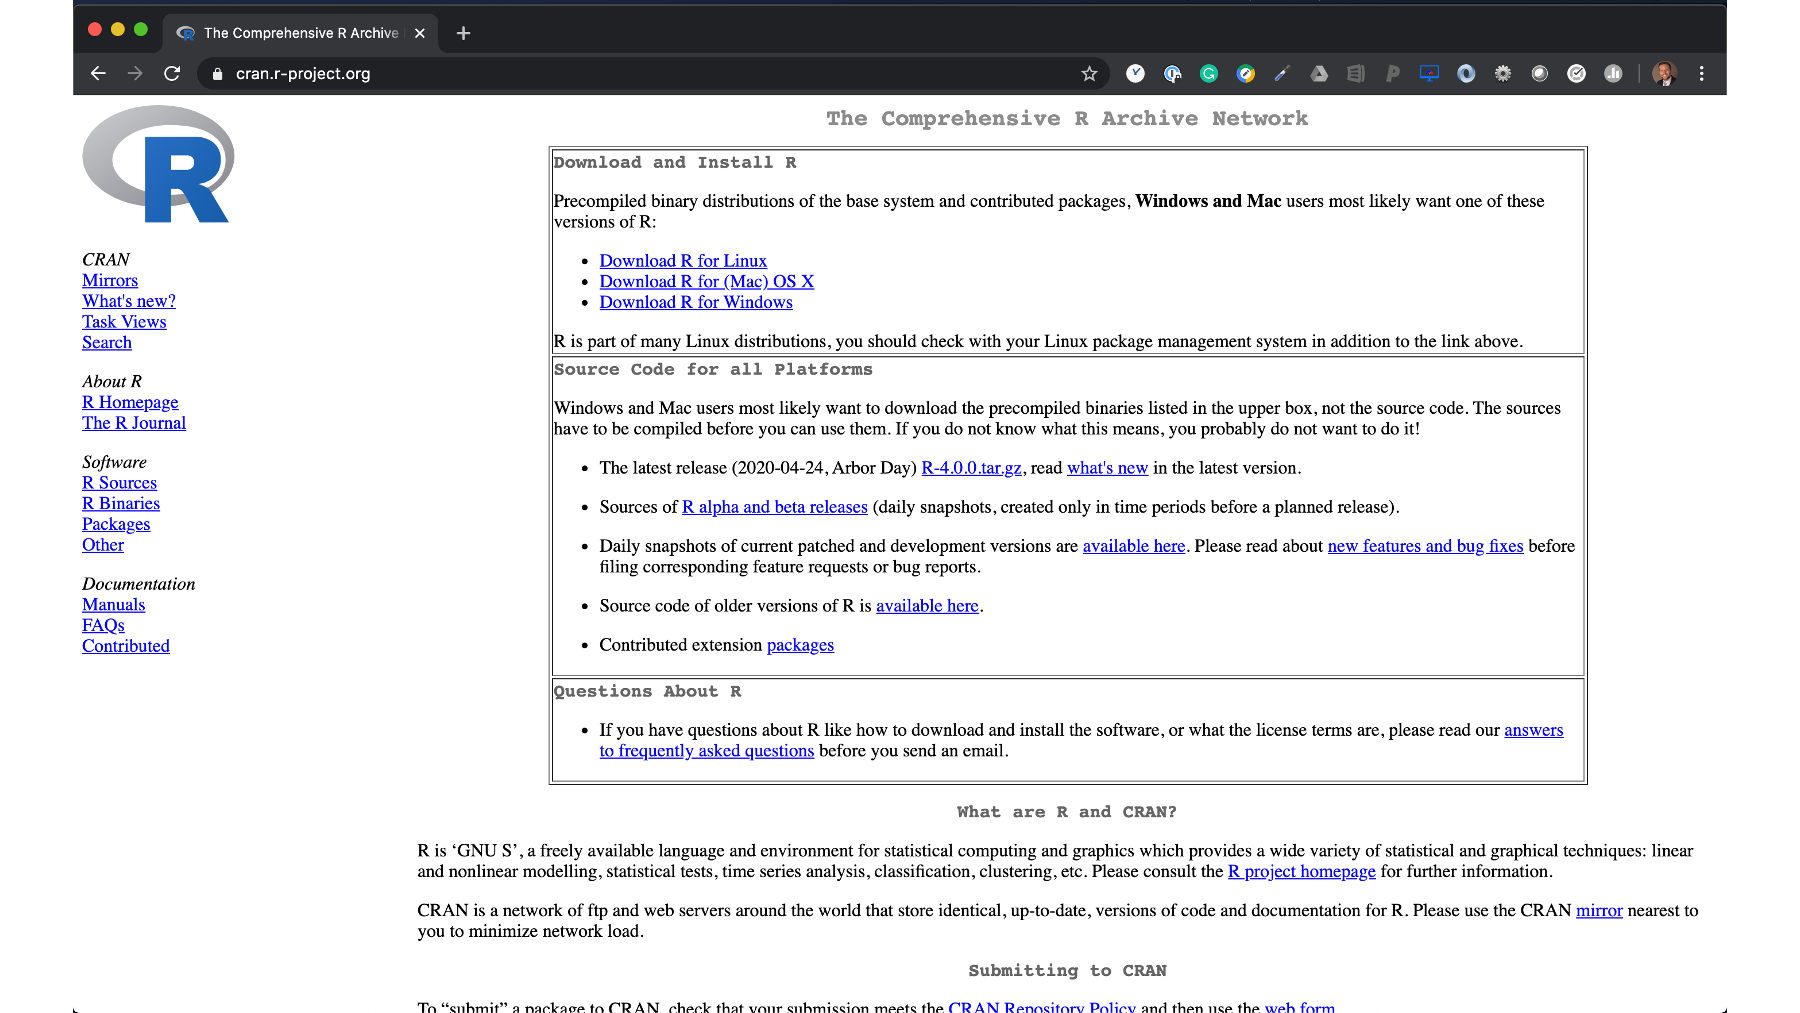
\includegraphics[keepaspectratio]{chapters/installing_r_and_rstudio/mac_cran.png}}

\textbf{Step 3:} Click on Download R for macOS.

\pandocbounded{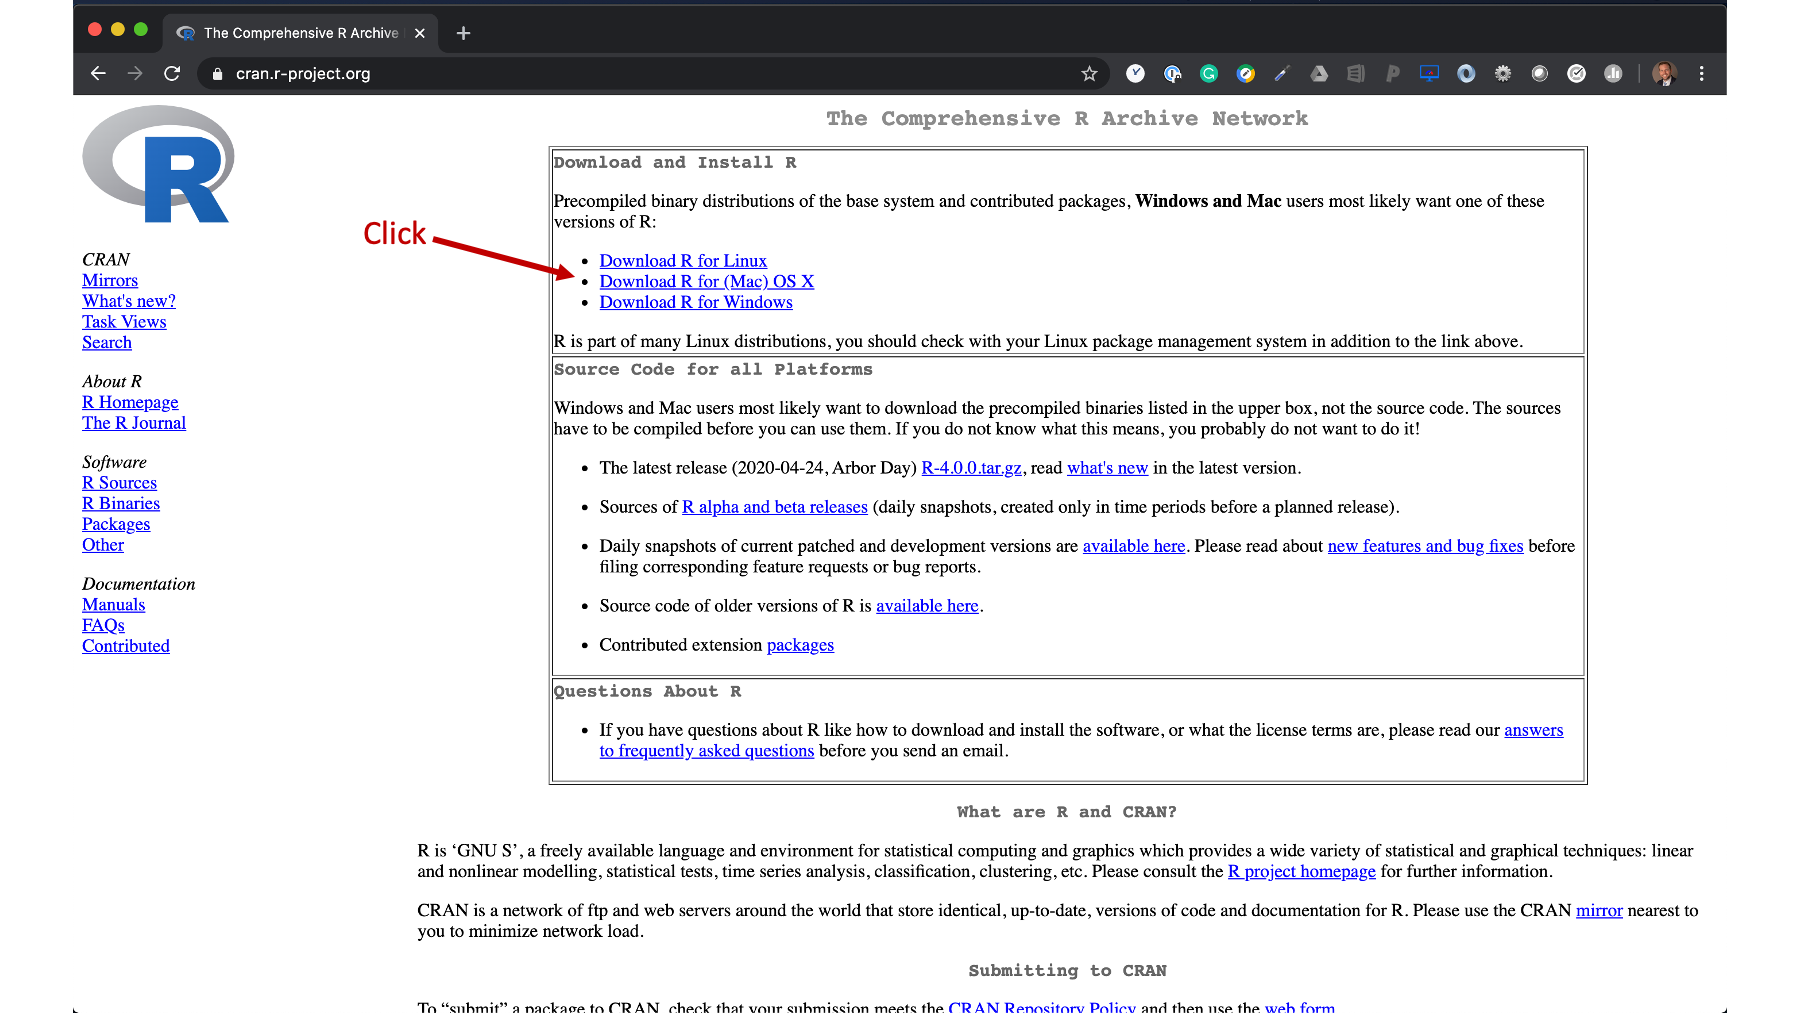
\includegraphics[keepaspectratio]{chapters/installing_r_and_rstudio/mac_download_r.png}}

\textbf{Step 4:} Click on the link for the latest version of R. As you
are reading this, the newest version may be different than the version
you see in this picture, but the location of the newest version should
be roughly in the same place -- the middle of the screen under ``Latest
release:''. After clicking the link, R should start to download to your
computer automatically.

\pandocbounded{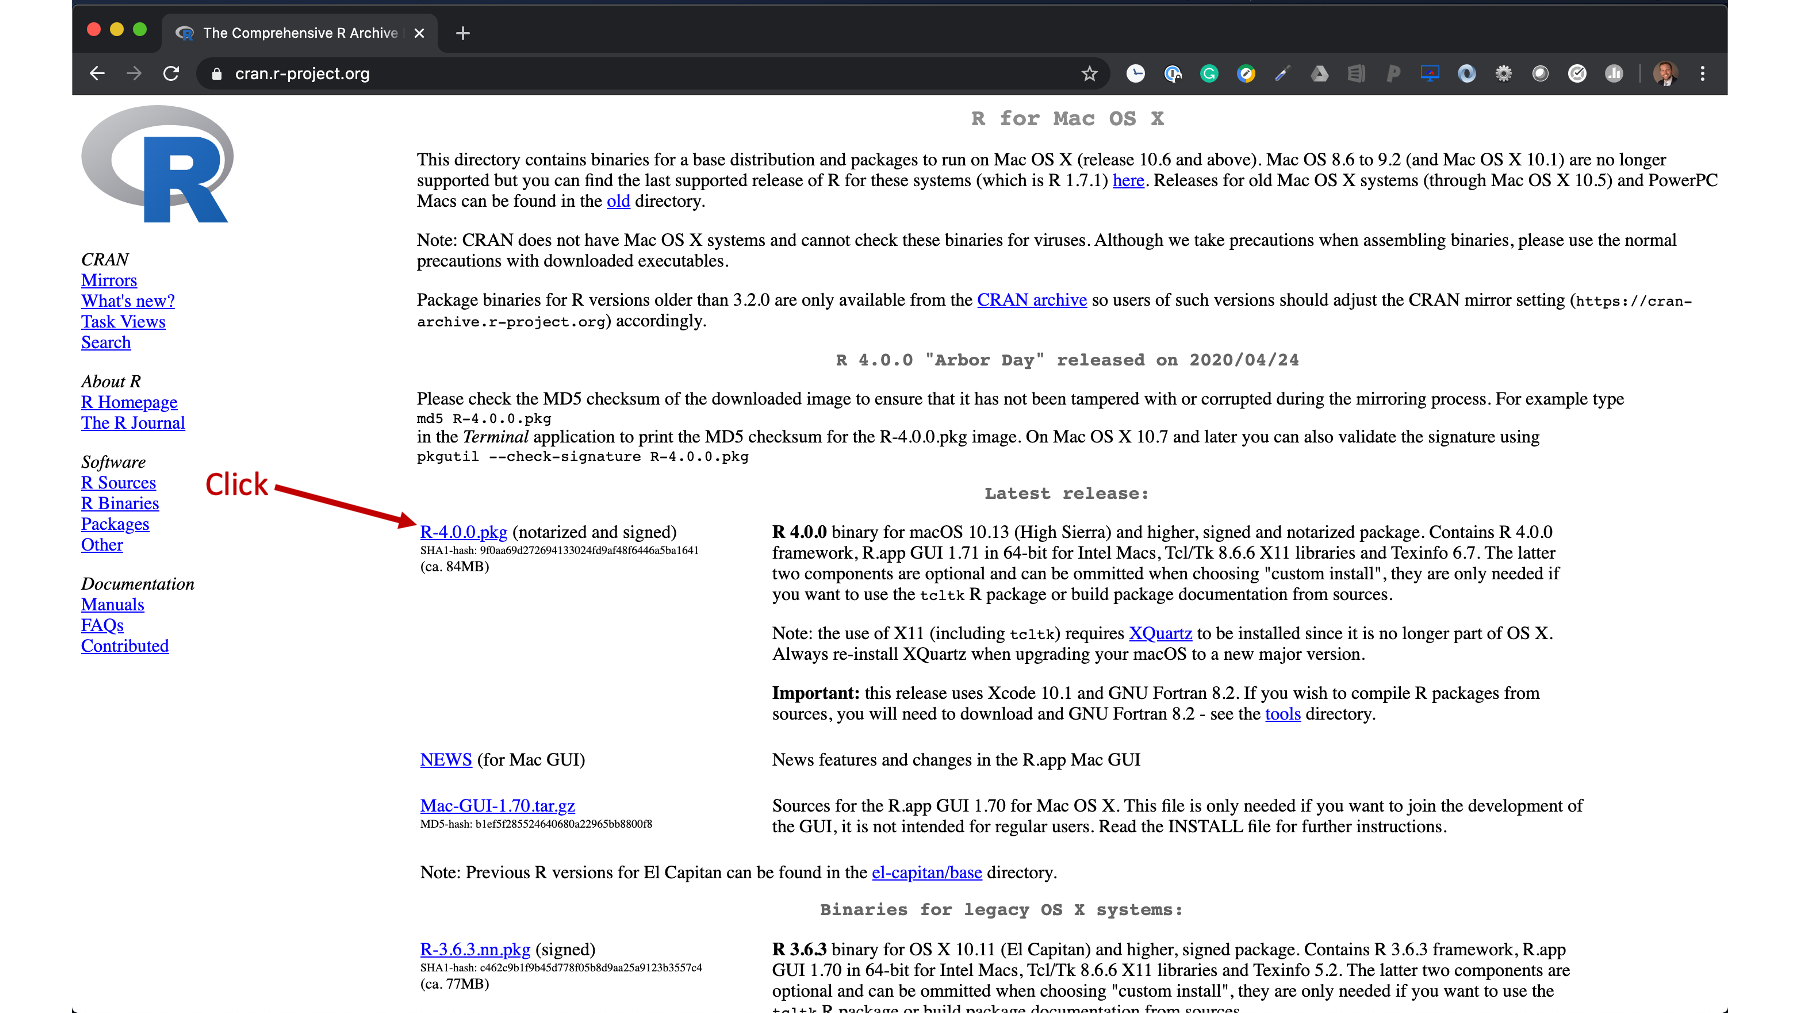
\includegraphics[keepaspectratio]{chapters/installing_r_and_rstudio/mac_r_version.png}}

\textbf{Step 5:} Locate the package file you just downloaded and double
click it. Unless you've changed your download settings, this file will
probably be in your ``downloads'' folder. That is the default location
for most web browsers. After you locate the file, just double click it.

\pandocbounded{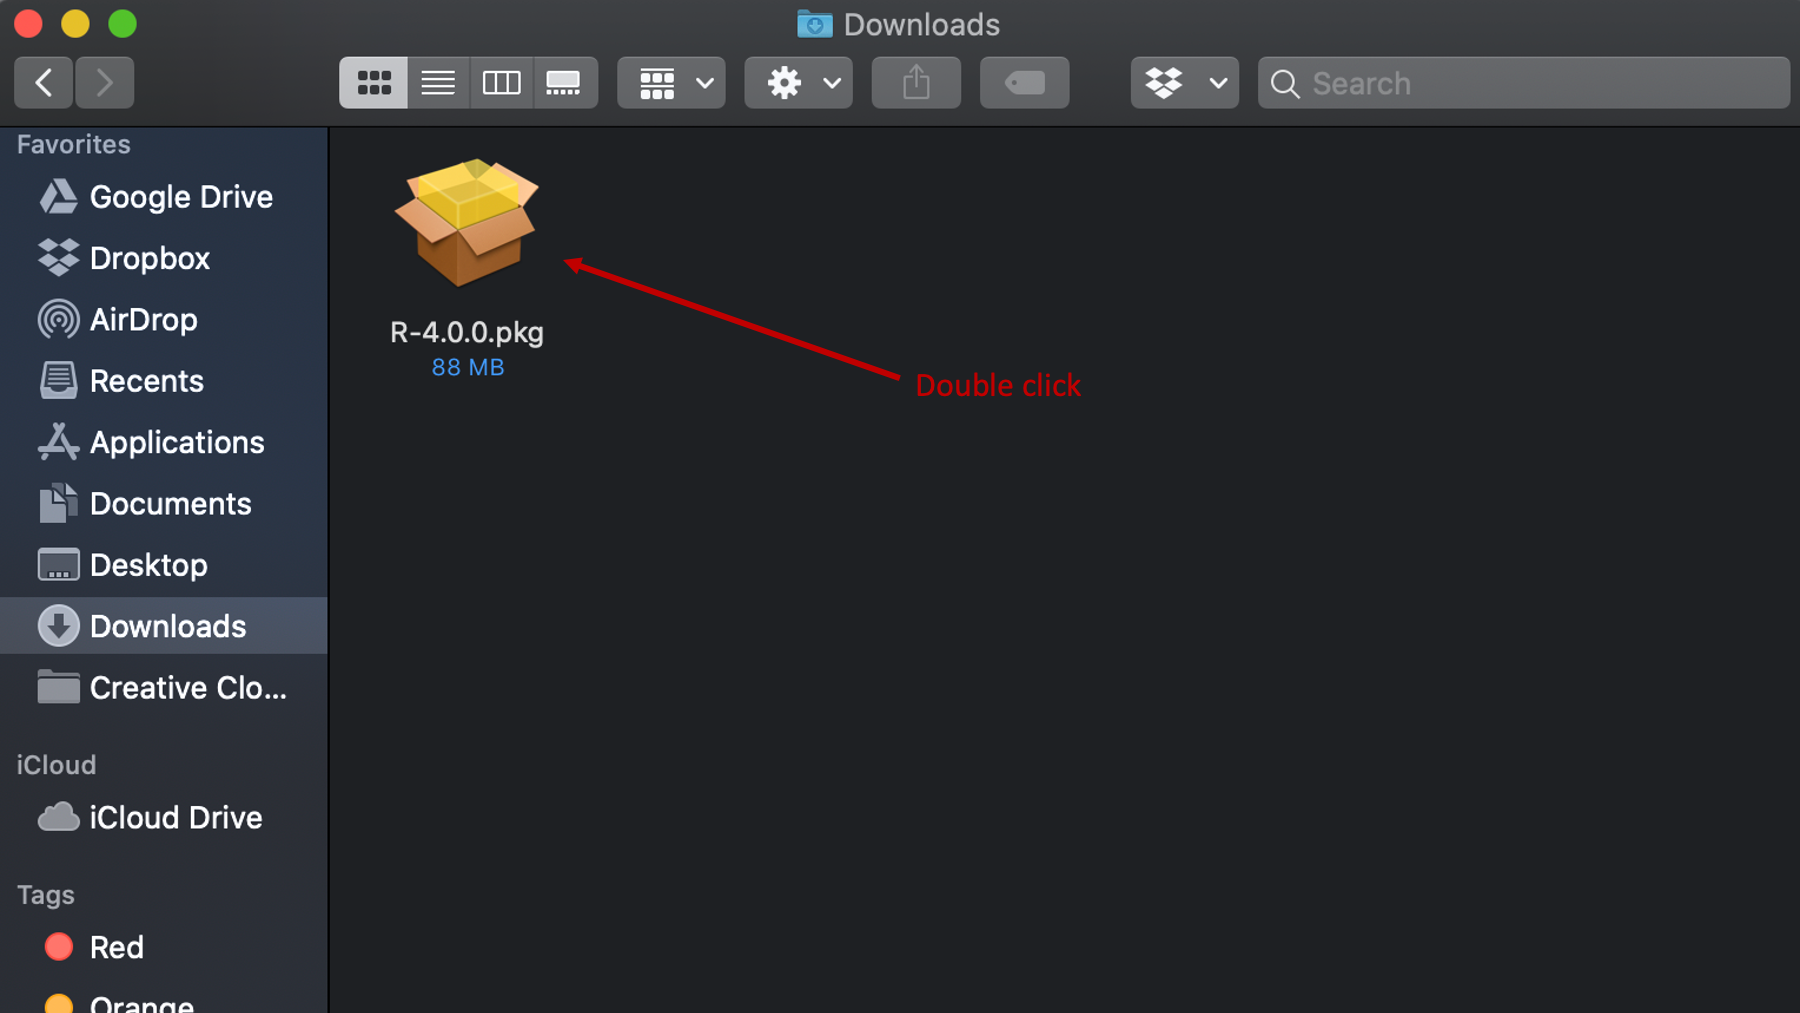
\includegraphics[keepaspectratio]{chapters/installing_r_and_rstudio/mac_install_r1.png}}

\textbf{Step 6:} A dialogue box will open and ask you to make some
decisions about how and where you want to install R on your computer. We
typically just click ``continue'' at every step without changing any of
the default options.

\pandocbounded{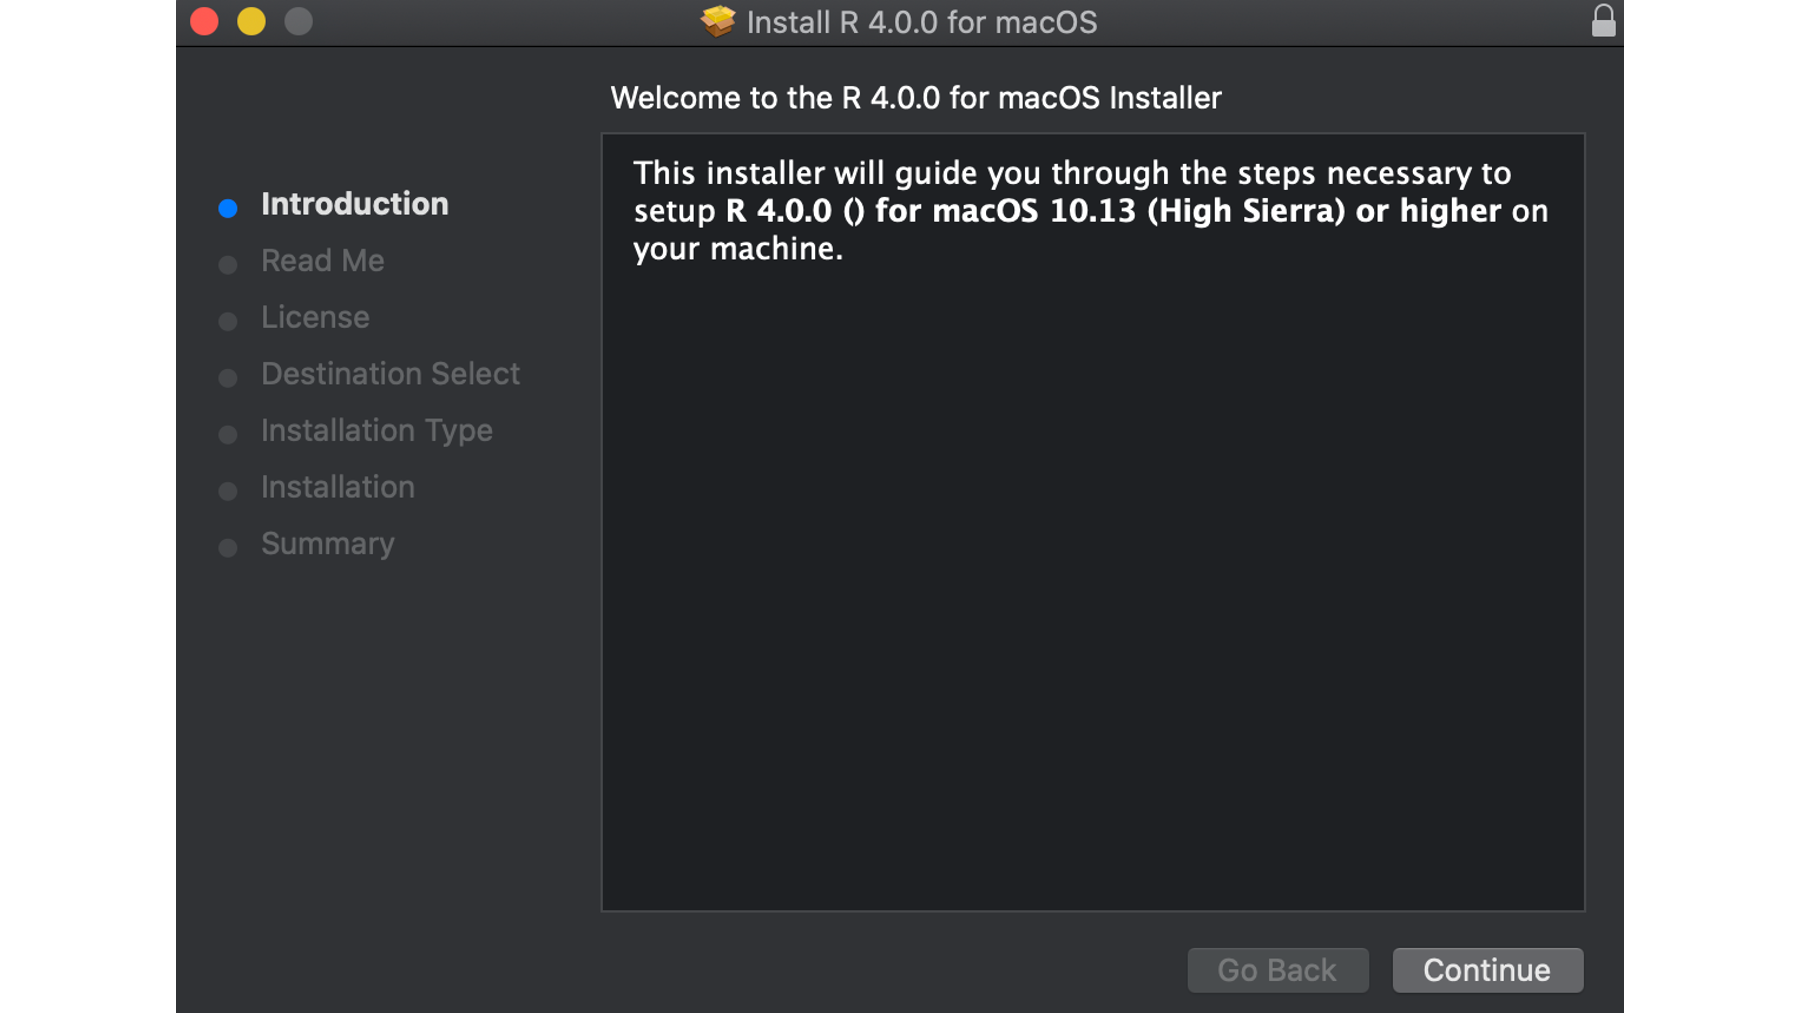
\includegraphics[keepaspectratio]{chapters/installing_r_and_rstudio/mac_install_r2.png}}

If R installed properly, you should now see it in your applications
folder.

\pandocbounded{
\includegraphics[keepaspectratio]{chapters/installing_r_and_rstudio/mac_view_r.png}}

\textbf{Step 7:} Now, we need to install the RStudio IDE. To do this,
navigate to the RStudio desktop download website, which is located at
https://posit.co/download/rstudio-desktop/. On that page, click the
button to download the latest version of RStudio for your computer. Note
that the website may look different that what you see in the screenshot
below because websites change over time.

\pandocbounded{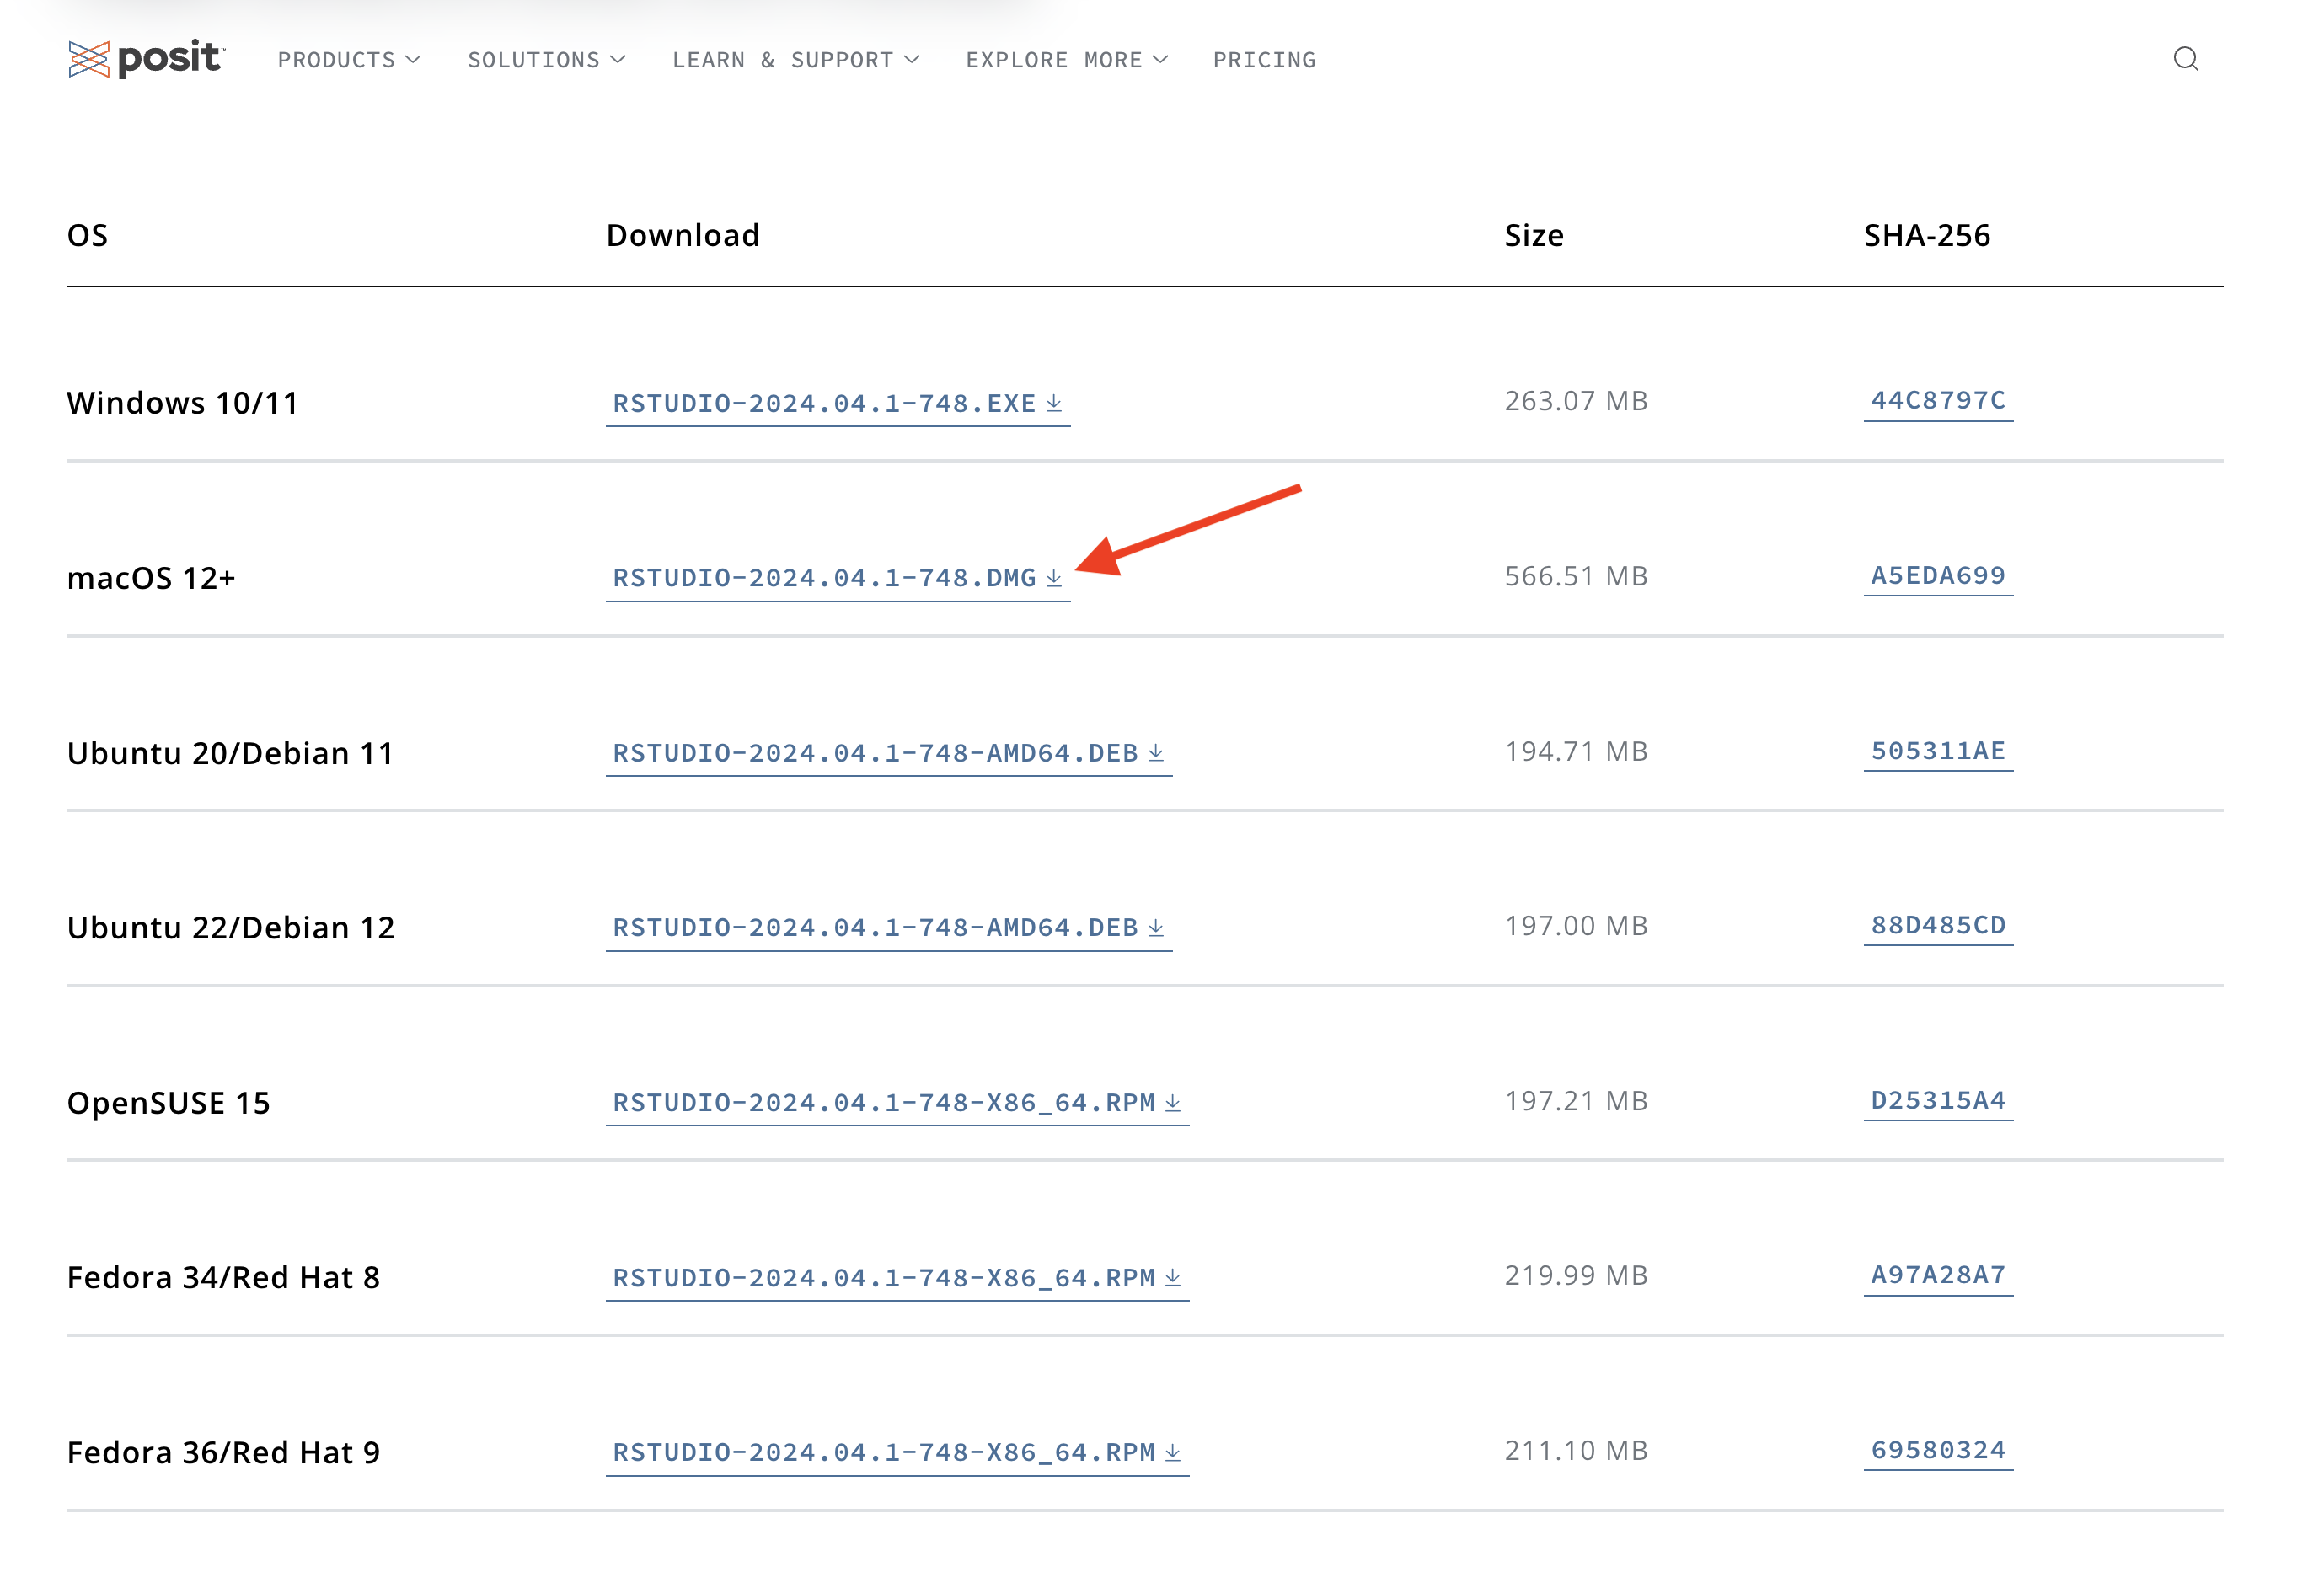
\includegraphics[keepaspectratio]{chapters/installing_r_and_rstudio/mac_download_rstudio1.png}}

\textbf{Step 8:} Again, locate the DMG file you just downloaded and
double click it. Unless you've changed your download settings, this file
should be in the same location as the R package file you already
downloaded.

\pandocbounded{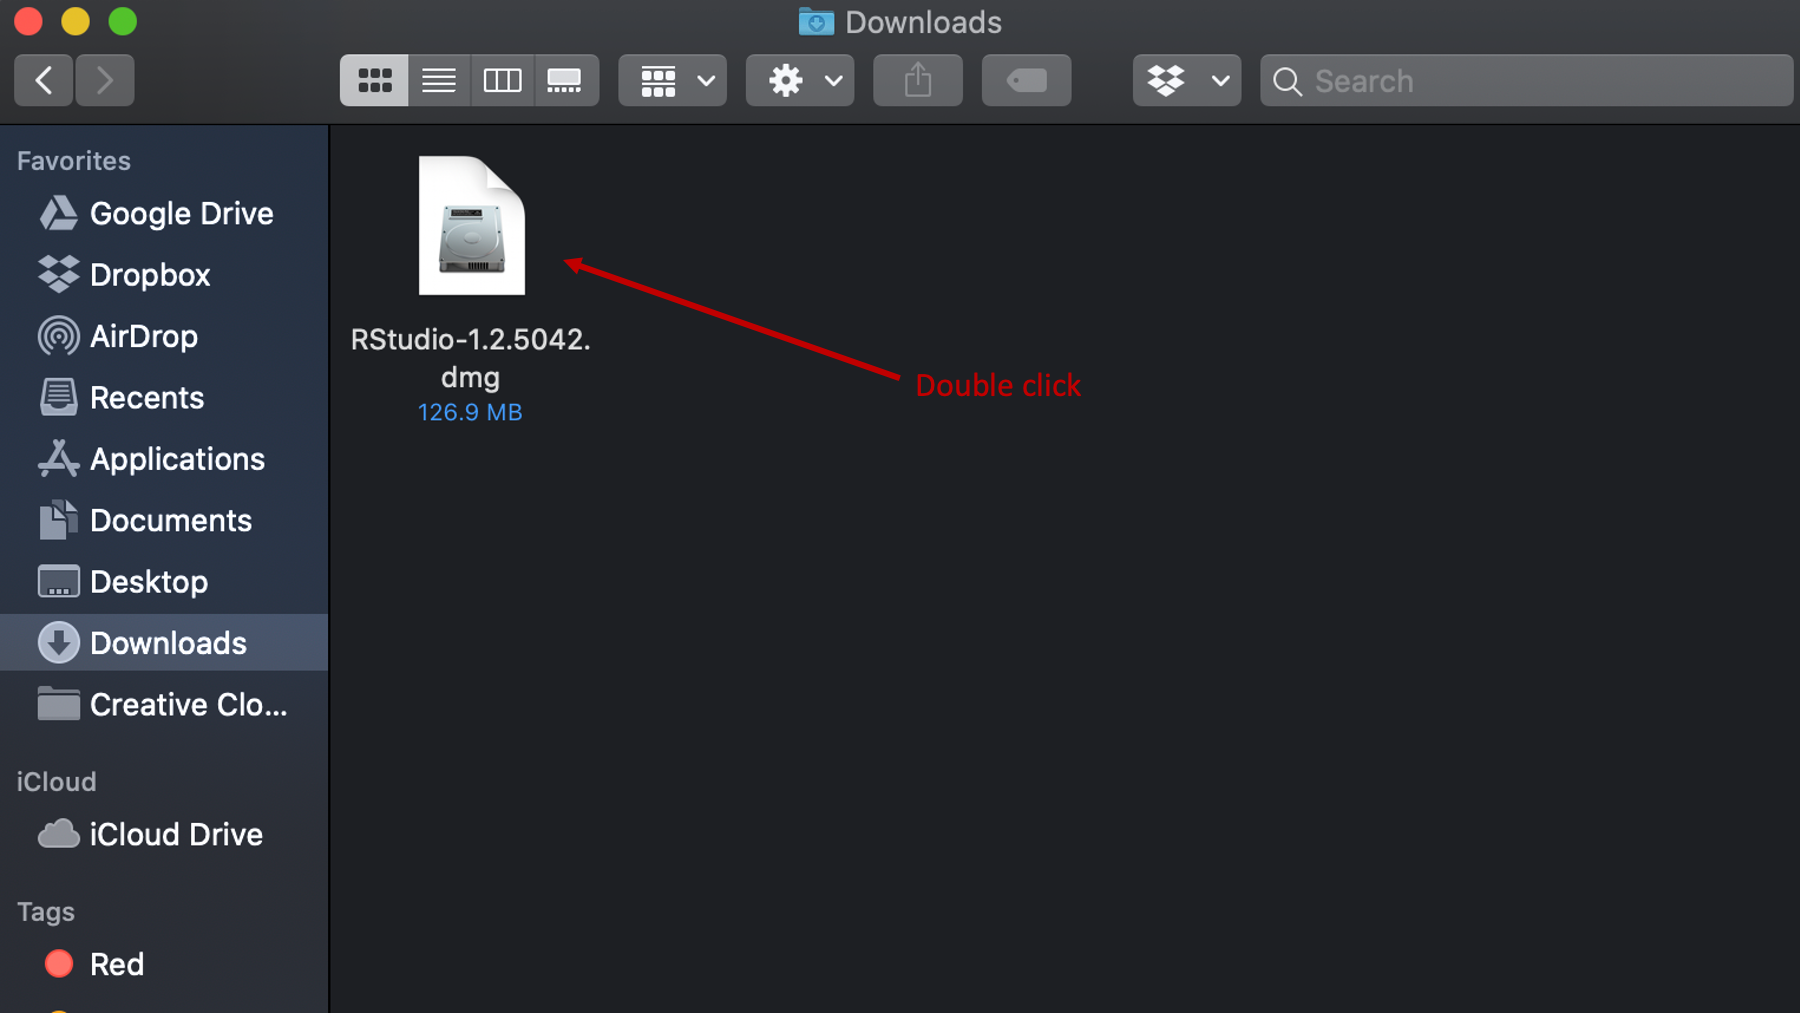
\includegraphics[keepaspectratio]{chapters/installing_r_and_rstudio/mac_install_rstudio1.png}}

\textbf{Step 9:} A new finder window should automatically pop up that
looks like the one you see below. Click on the RStudio icon and drag it
into the Applications folder.

\pandocbounded{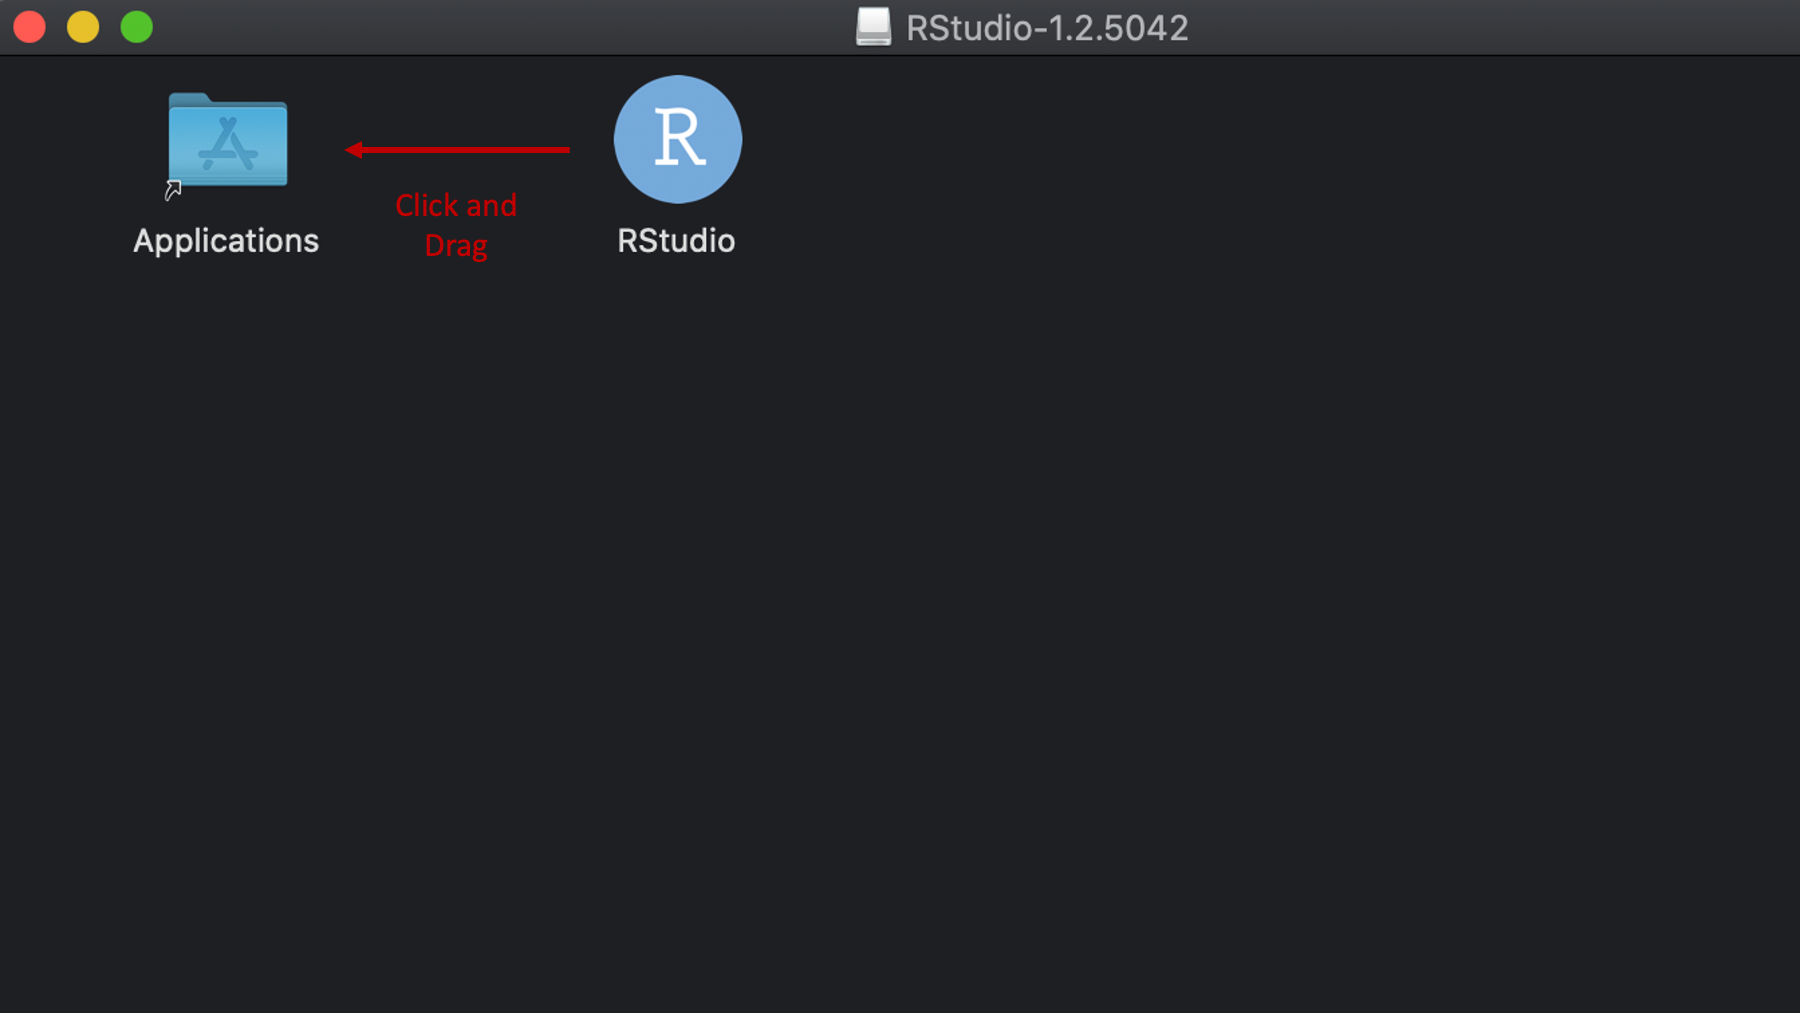
\includegraphics[keepaspectratio]{chapters/installing_r_and_rstudio/mac_install_rstudio2.png}}

You should now see RStudio in your Applications folder. Double click the
icon to open RStudio.

\pandocbounded{
\includegraphics[keepaspectratio]{chapters/installing_r_and_rstudio/mac_open_rstudio.png}}

If this warning pops up, just click Open.

\pandocbounded{
\includegraphics[keepaspectratio]{chapters/installing_r_and_rstudio/mac_open_warning.png}}

The RStudio IDE should open and look something like the window you see
here. If so, you are good to go! 🎉

\pandocbounded{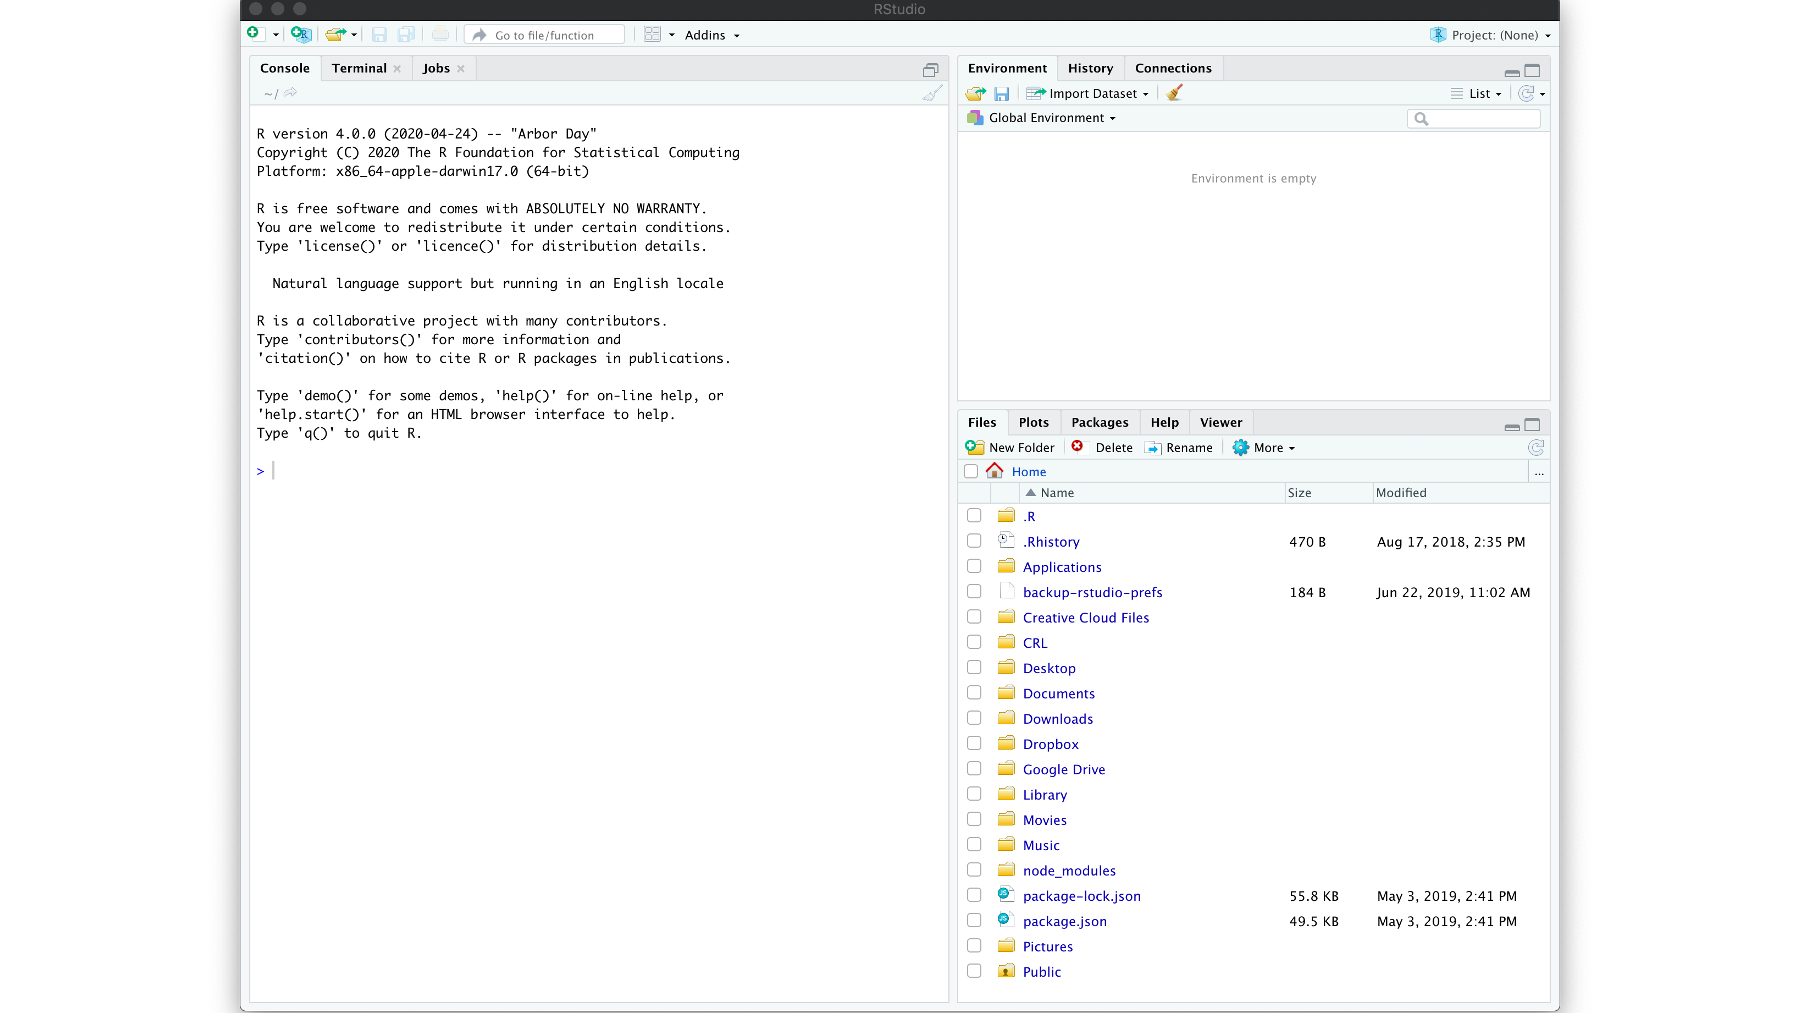
\includegraphics[keepaspectratio]{chapters/installing_r_and_rstudio/mac_view_rstudio.png}}

\section{Download and install on a
PC}\label{download-and-install-on-a-pc}

\textbf{Step 2:} Navigate to the Comprehensive R Archive Network (CRAN),
which is located at https://cran.r-project.org/.

\pandocbounded{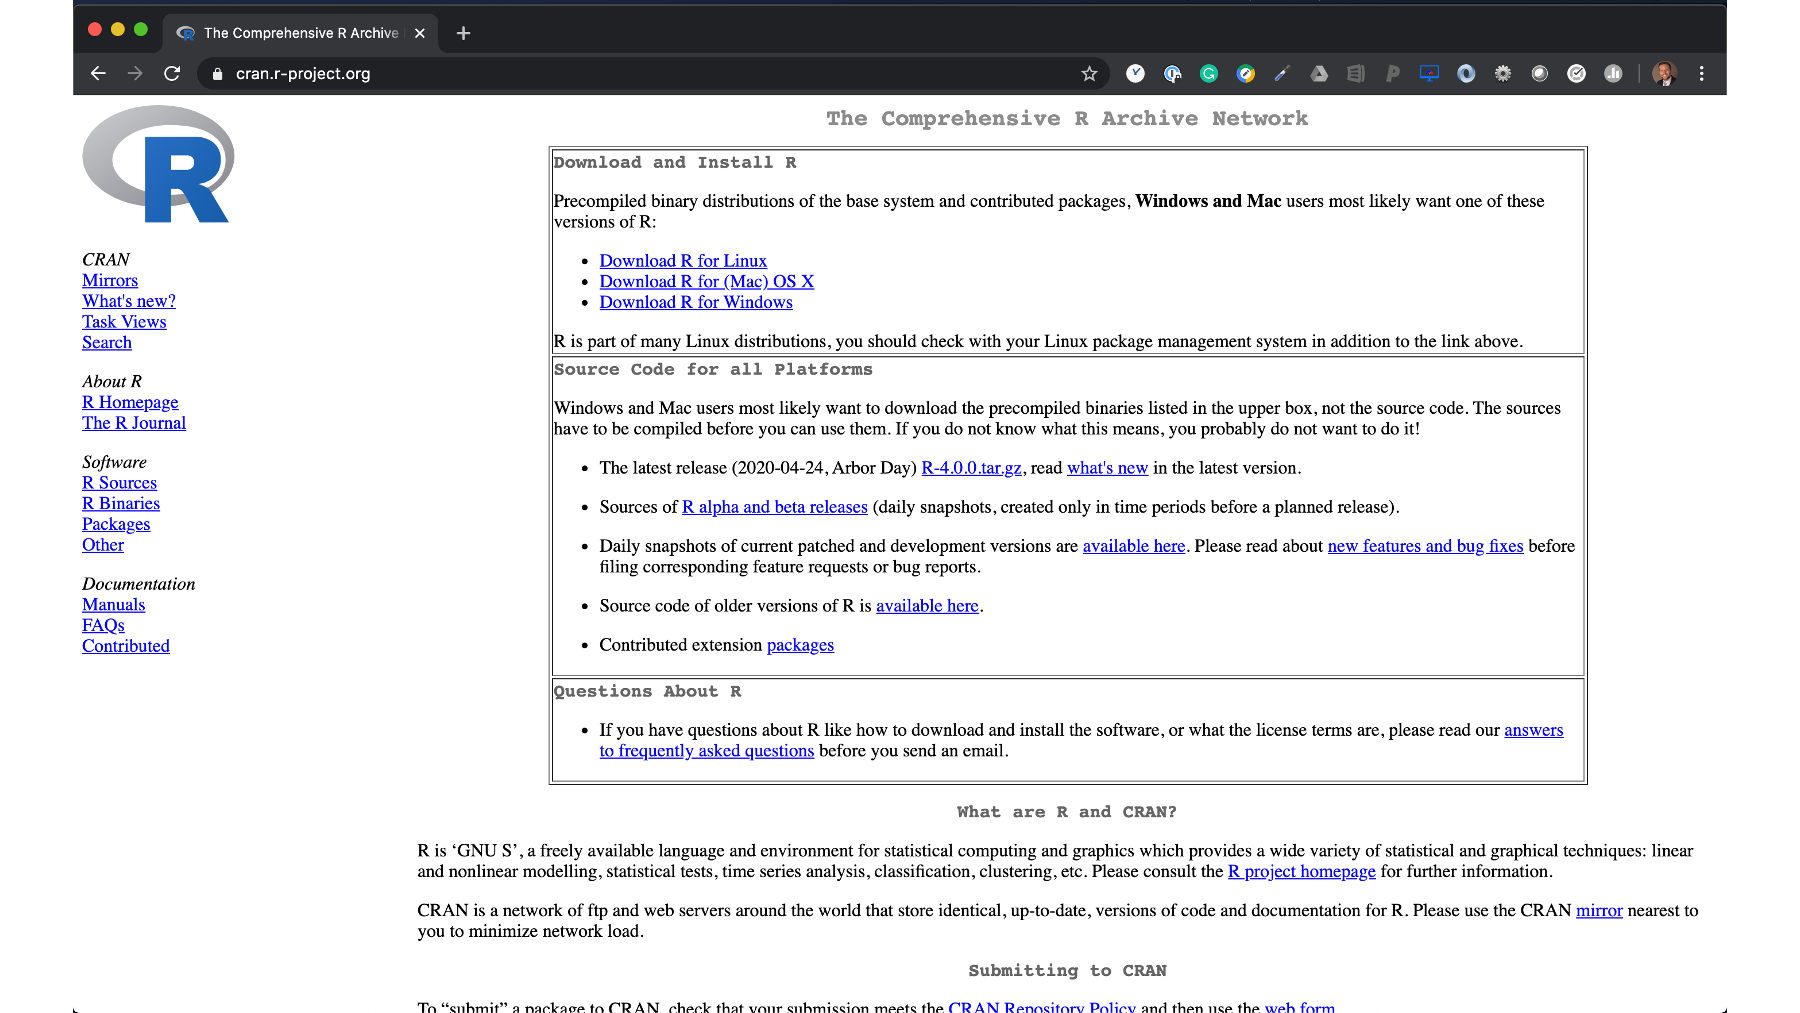
\includegraphics[keepaspectratio]{chapters/installing_r_and_rstudio/pc_cran.png}}

\textbf{Step 3:} Click on Download R for Windows.

\pandocbounded{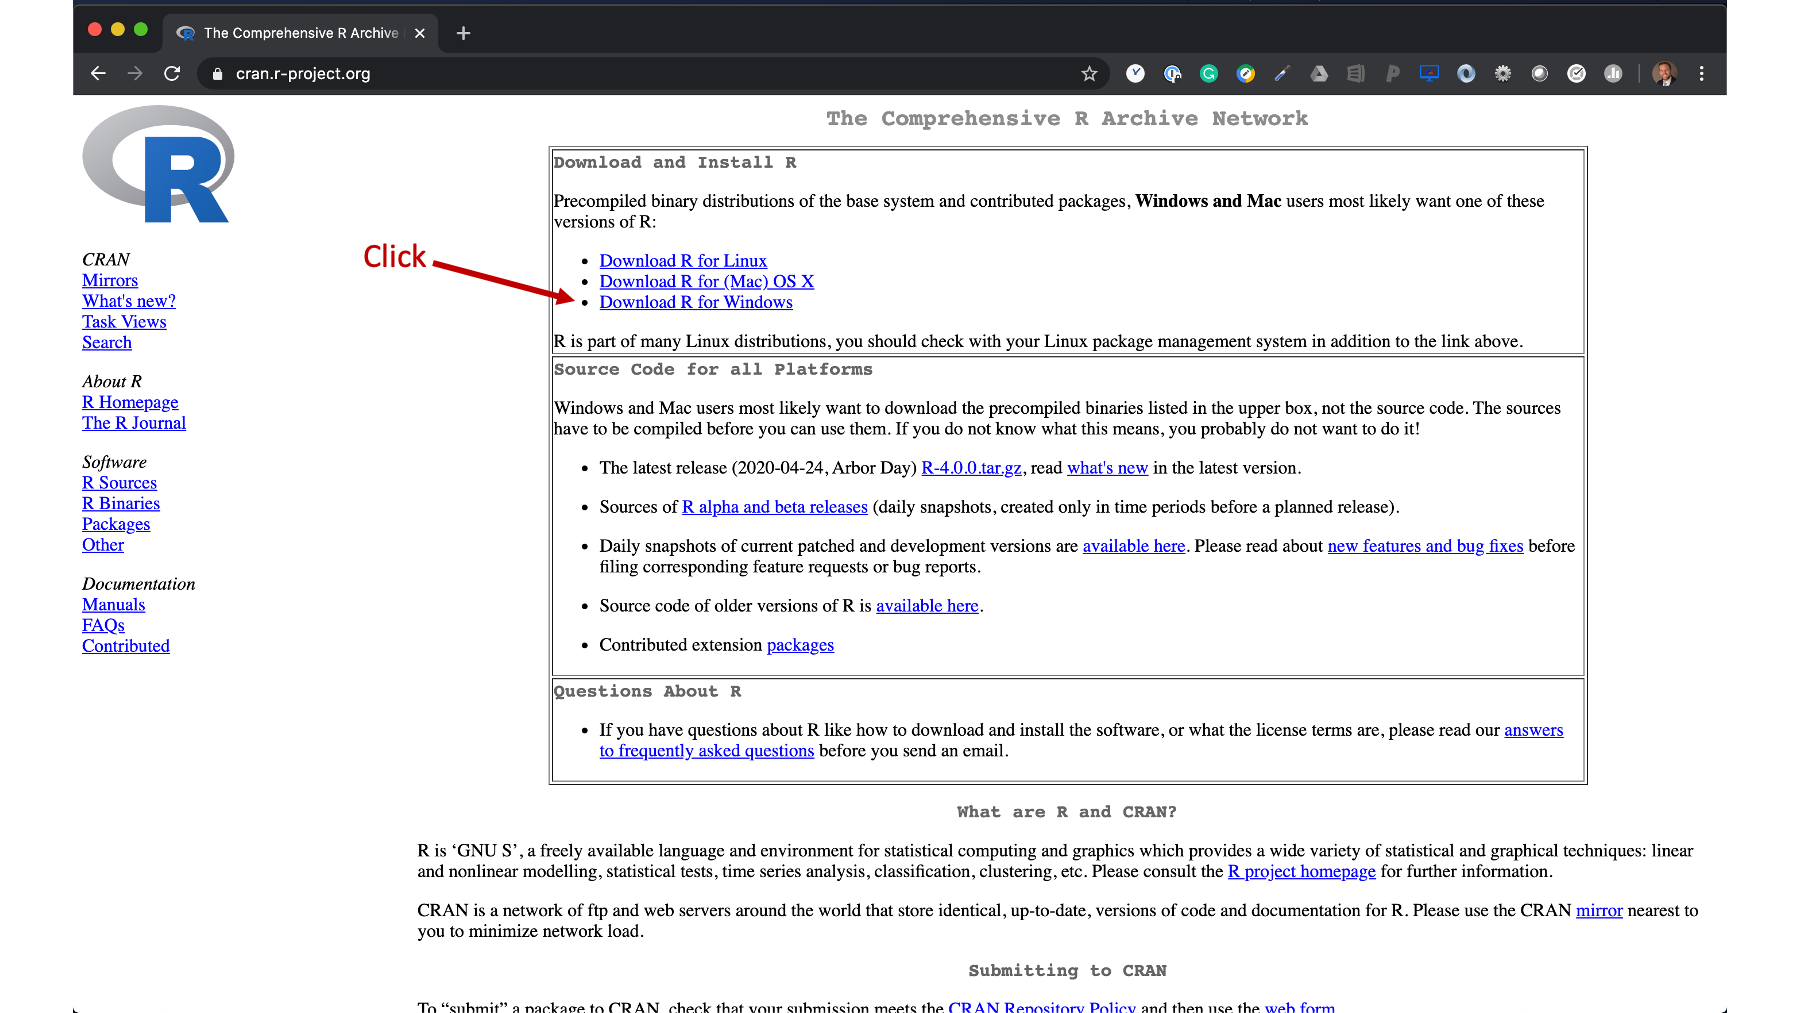
\includegraphics[keepaspectratio]{chapters/installing_r_and_rstudio/pc_download_r1.png}}

\textbf{Step 4:} Click on the base link.

\pandocbounded{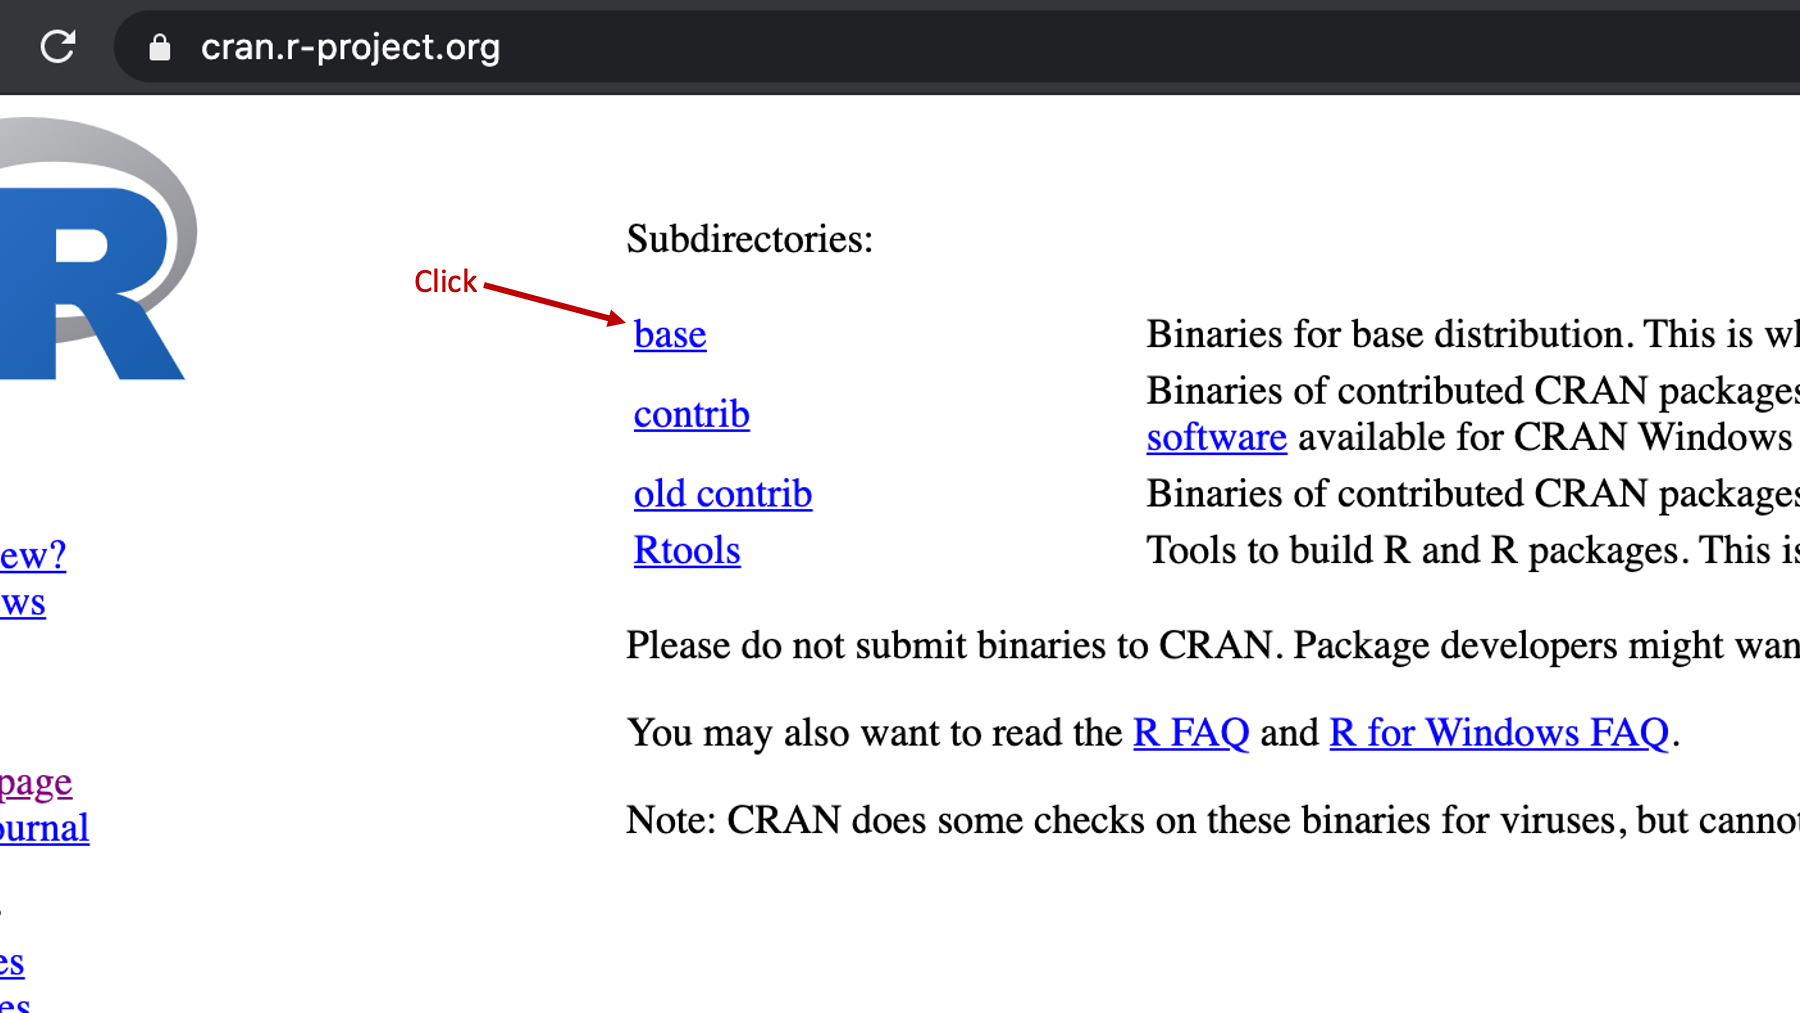
\includegraphics[keepaspectratio]{chapters/installing_r_and_rstudio/pc_download_r2.png}}

\textbf{Step 5:} Click on the link for the latest version of R. As you
are reading this, the newest version may be different than the version
you see in this picture, but the location of the newest version should
be roughly the same. After clicking, R should start to download to your
computer.

\pandocbounded{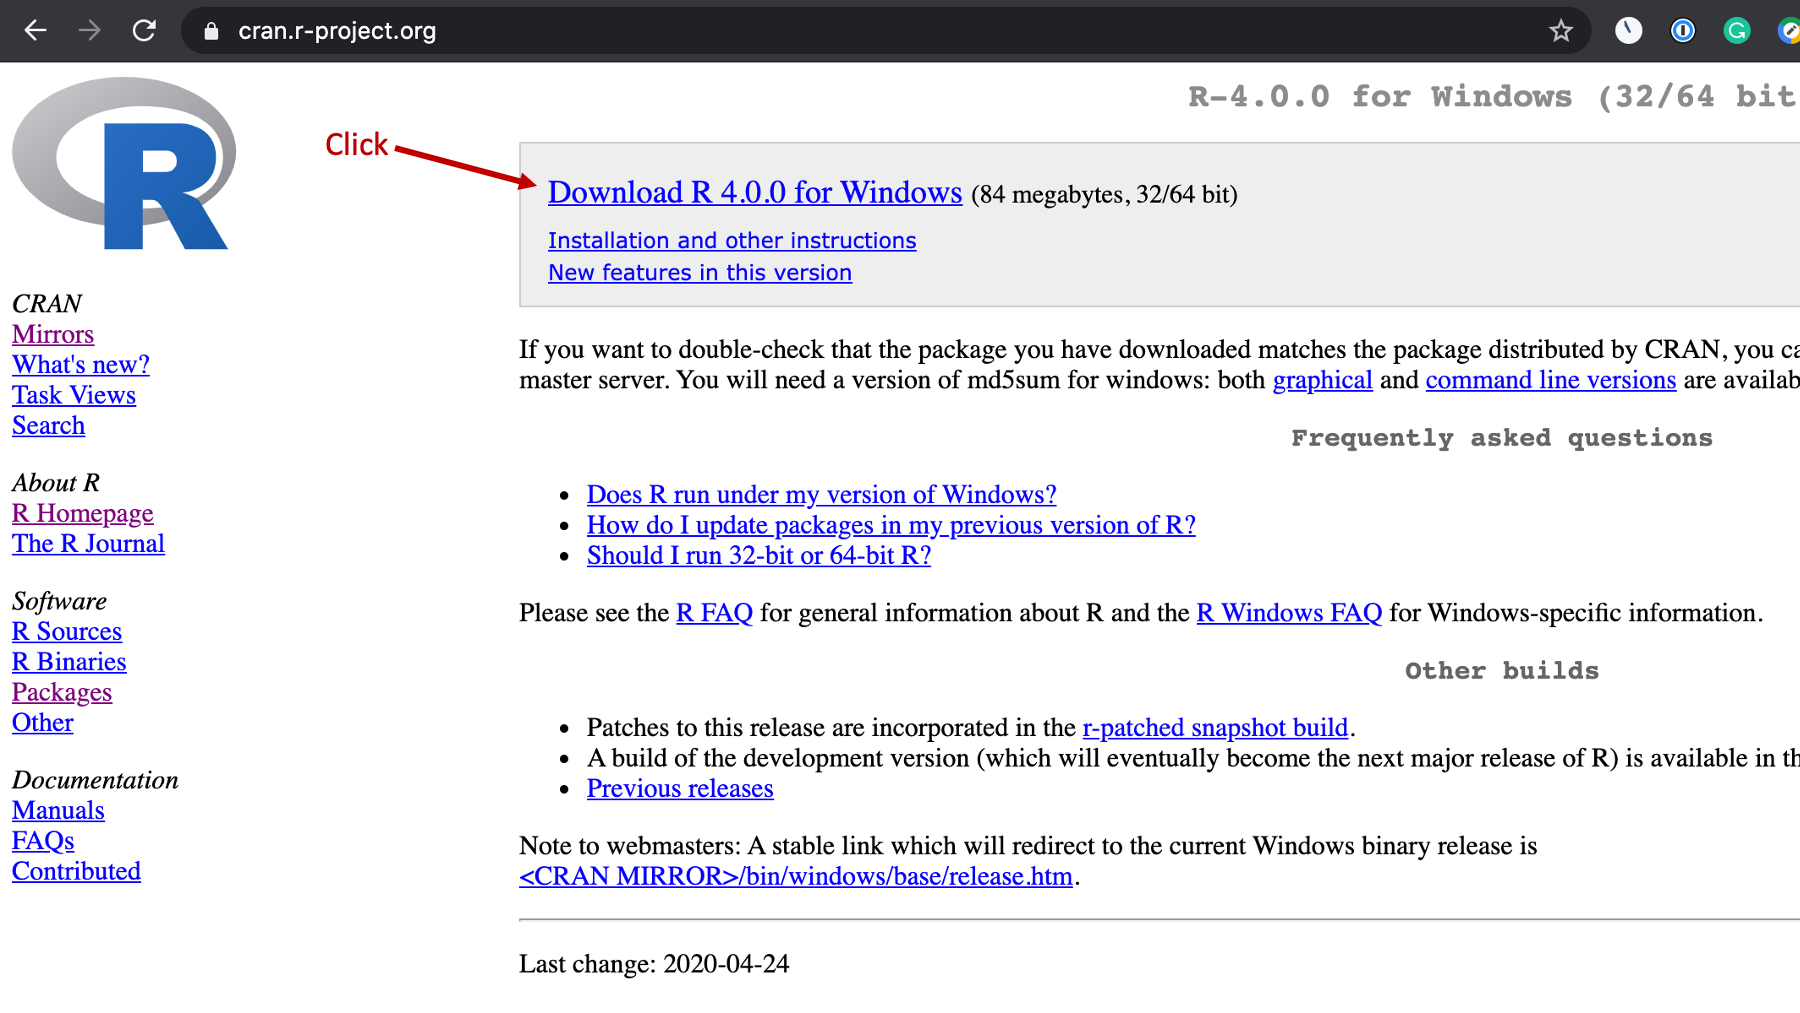
\includegraphics[keepaspectratio]{chapters/installing_r_and_rstudio/pc_download_r3.png}}

\textbf{Step 6:} Locate the installation file you just downloaded and
double click it. Unless you've changed your download settings, this file
will probably be in your downloads folder. That is the default location
for most web browsers.

\pandocbounded{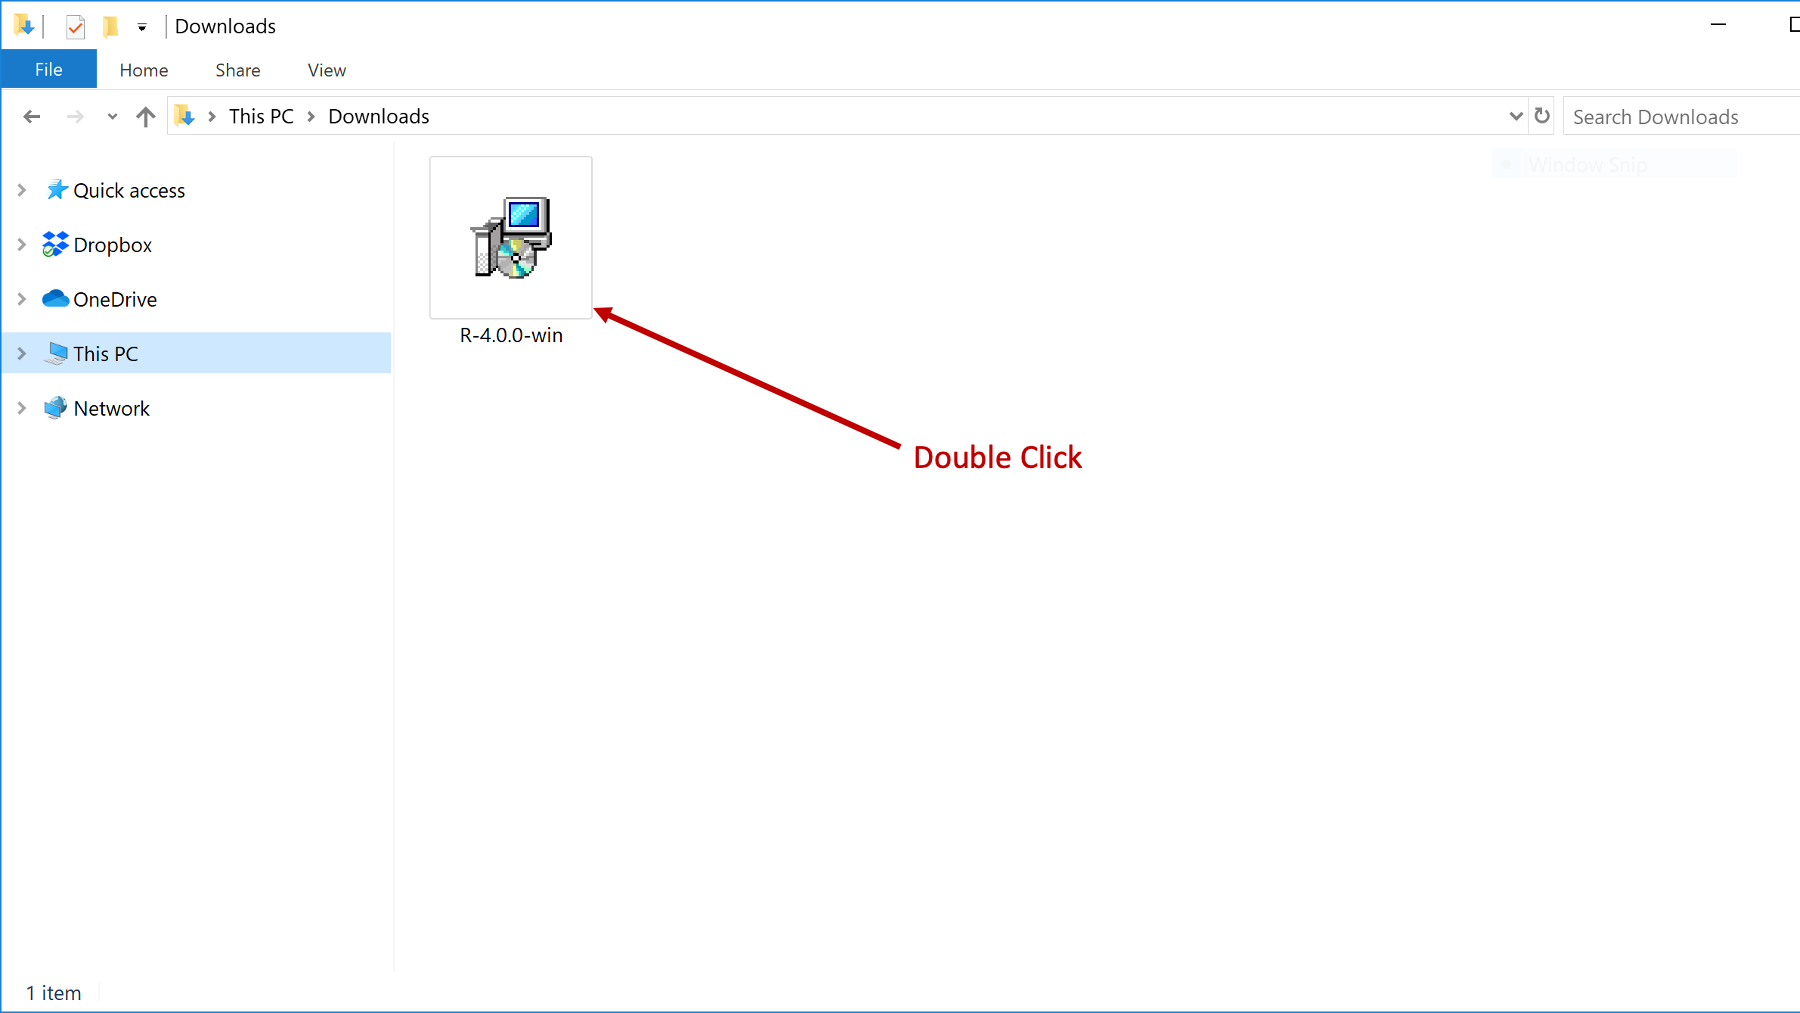
\includegraphics[keepaspectratio]{chapters/installing_r_and_rstudio/pc_install_r1.png}}

\textbf{Step 7:} A dialogue box will open that asks you to make some
decisions about how and where you want to install R on your computer. We
typically just click ``Next'' at every step without changing any of the
default options.

\pandocbounded{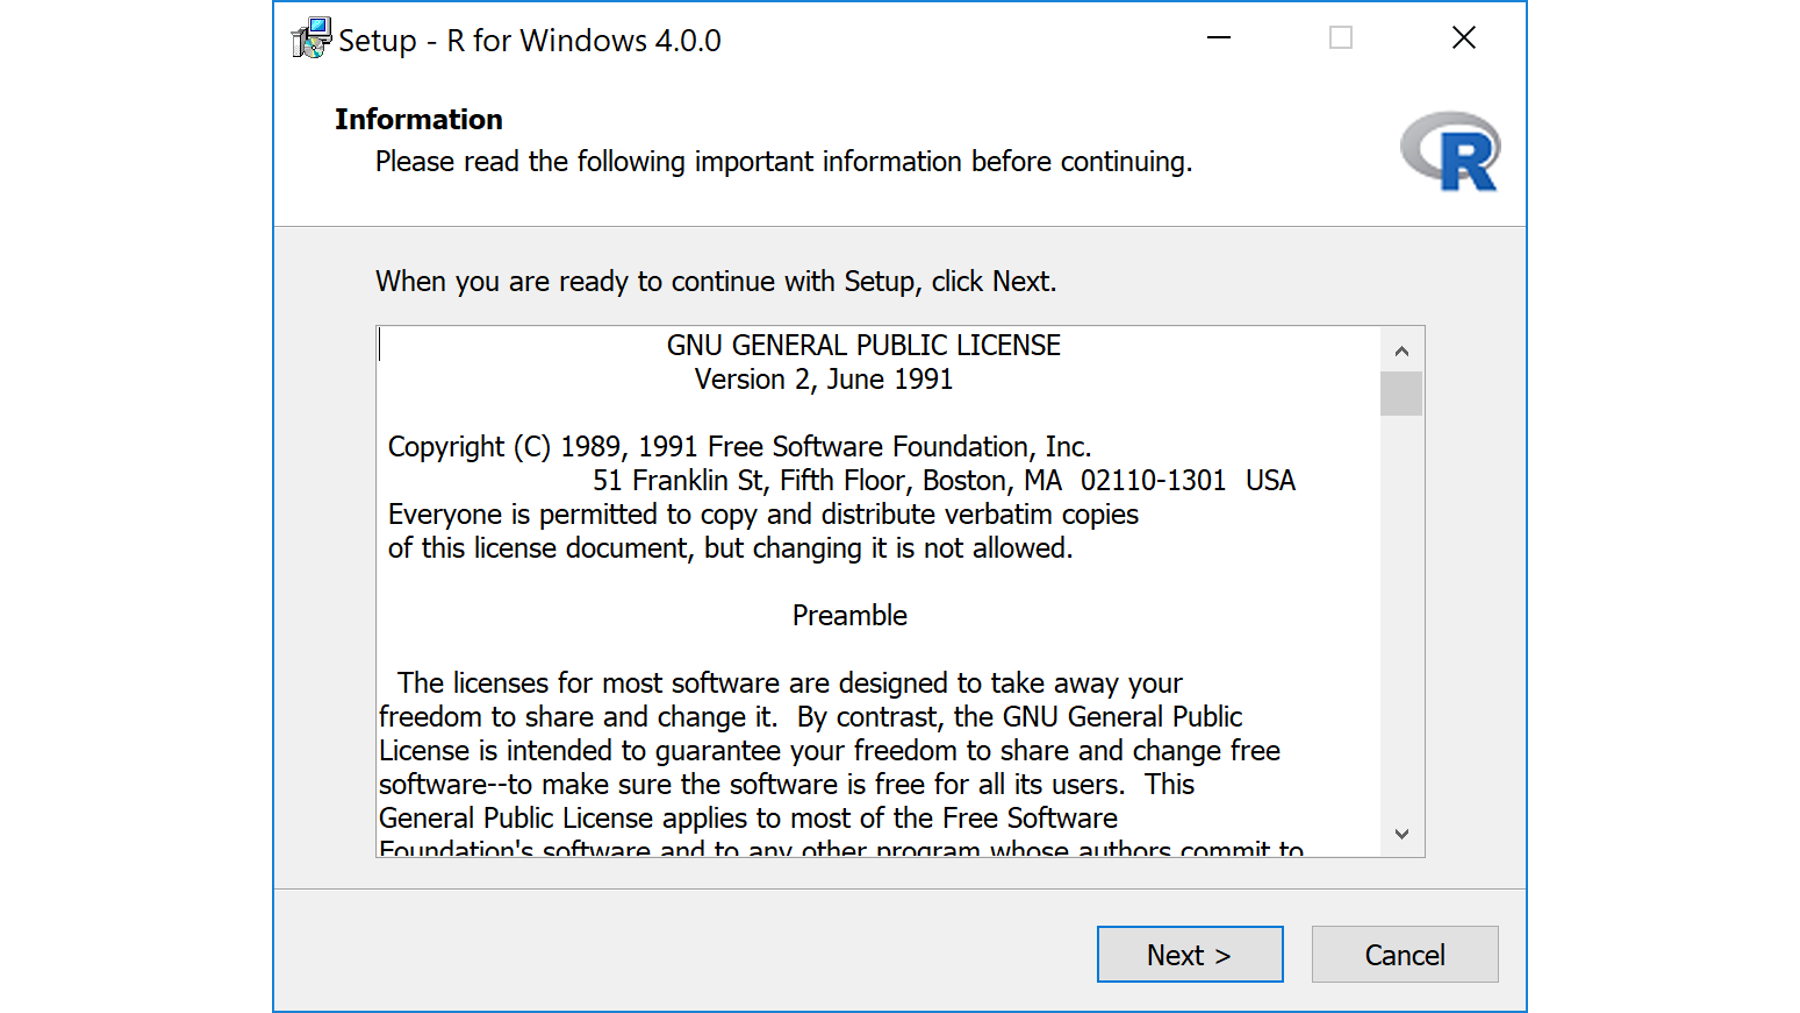
\includegraphics[keepaspectratio]{chapters/installing_r_and_rstudio/pc_install_r2.png}}

If R installed properly, you should now see it in the Windows start
menu.

\pandocbounded{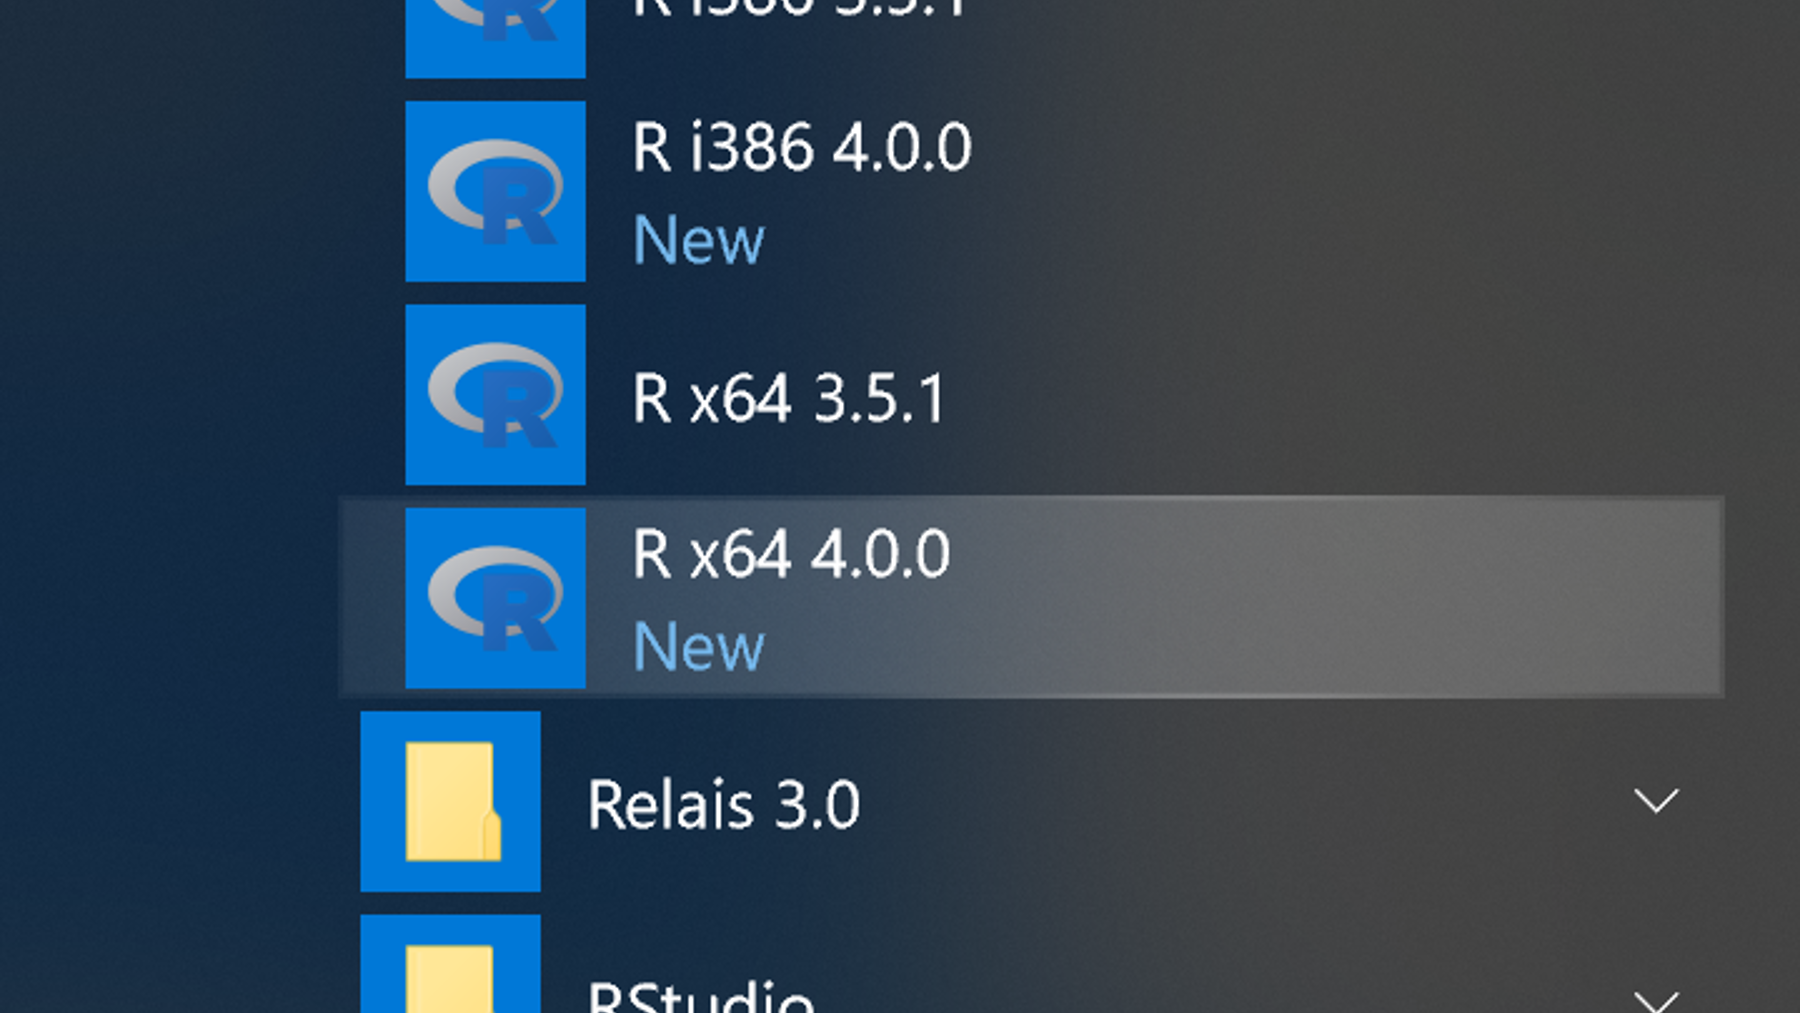
\includegraphics[keepaspectratio]{chapters/installing_r_and_rstudio/pc_view_r.png}}

\textbf{Step 8:} Now, we need to install the RStudio IDE. To do this,
navigate to the RStudio desktop download website, which is located at
https://posit.co/download/rstudio-desktop/. On that page, click the
button to download the latest version of RStudio for your computer. Note
that the website may look different that what you see in the screenshot
below because websites change over time.

\pandocbounded{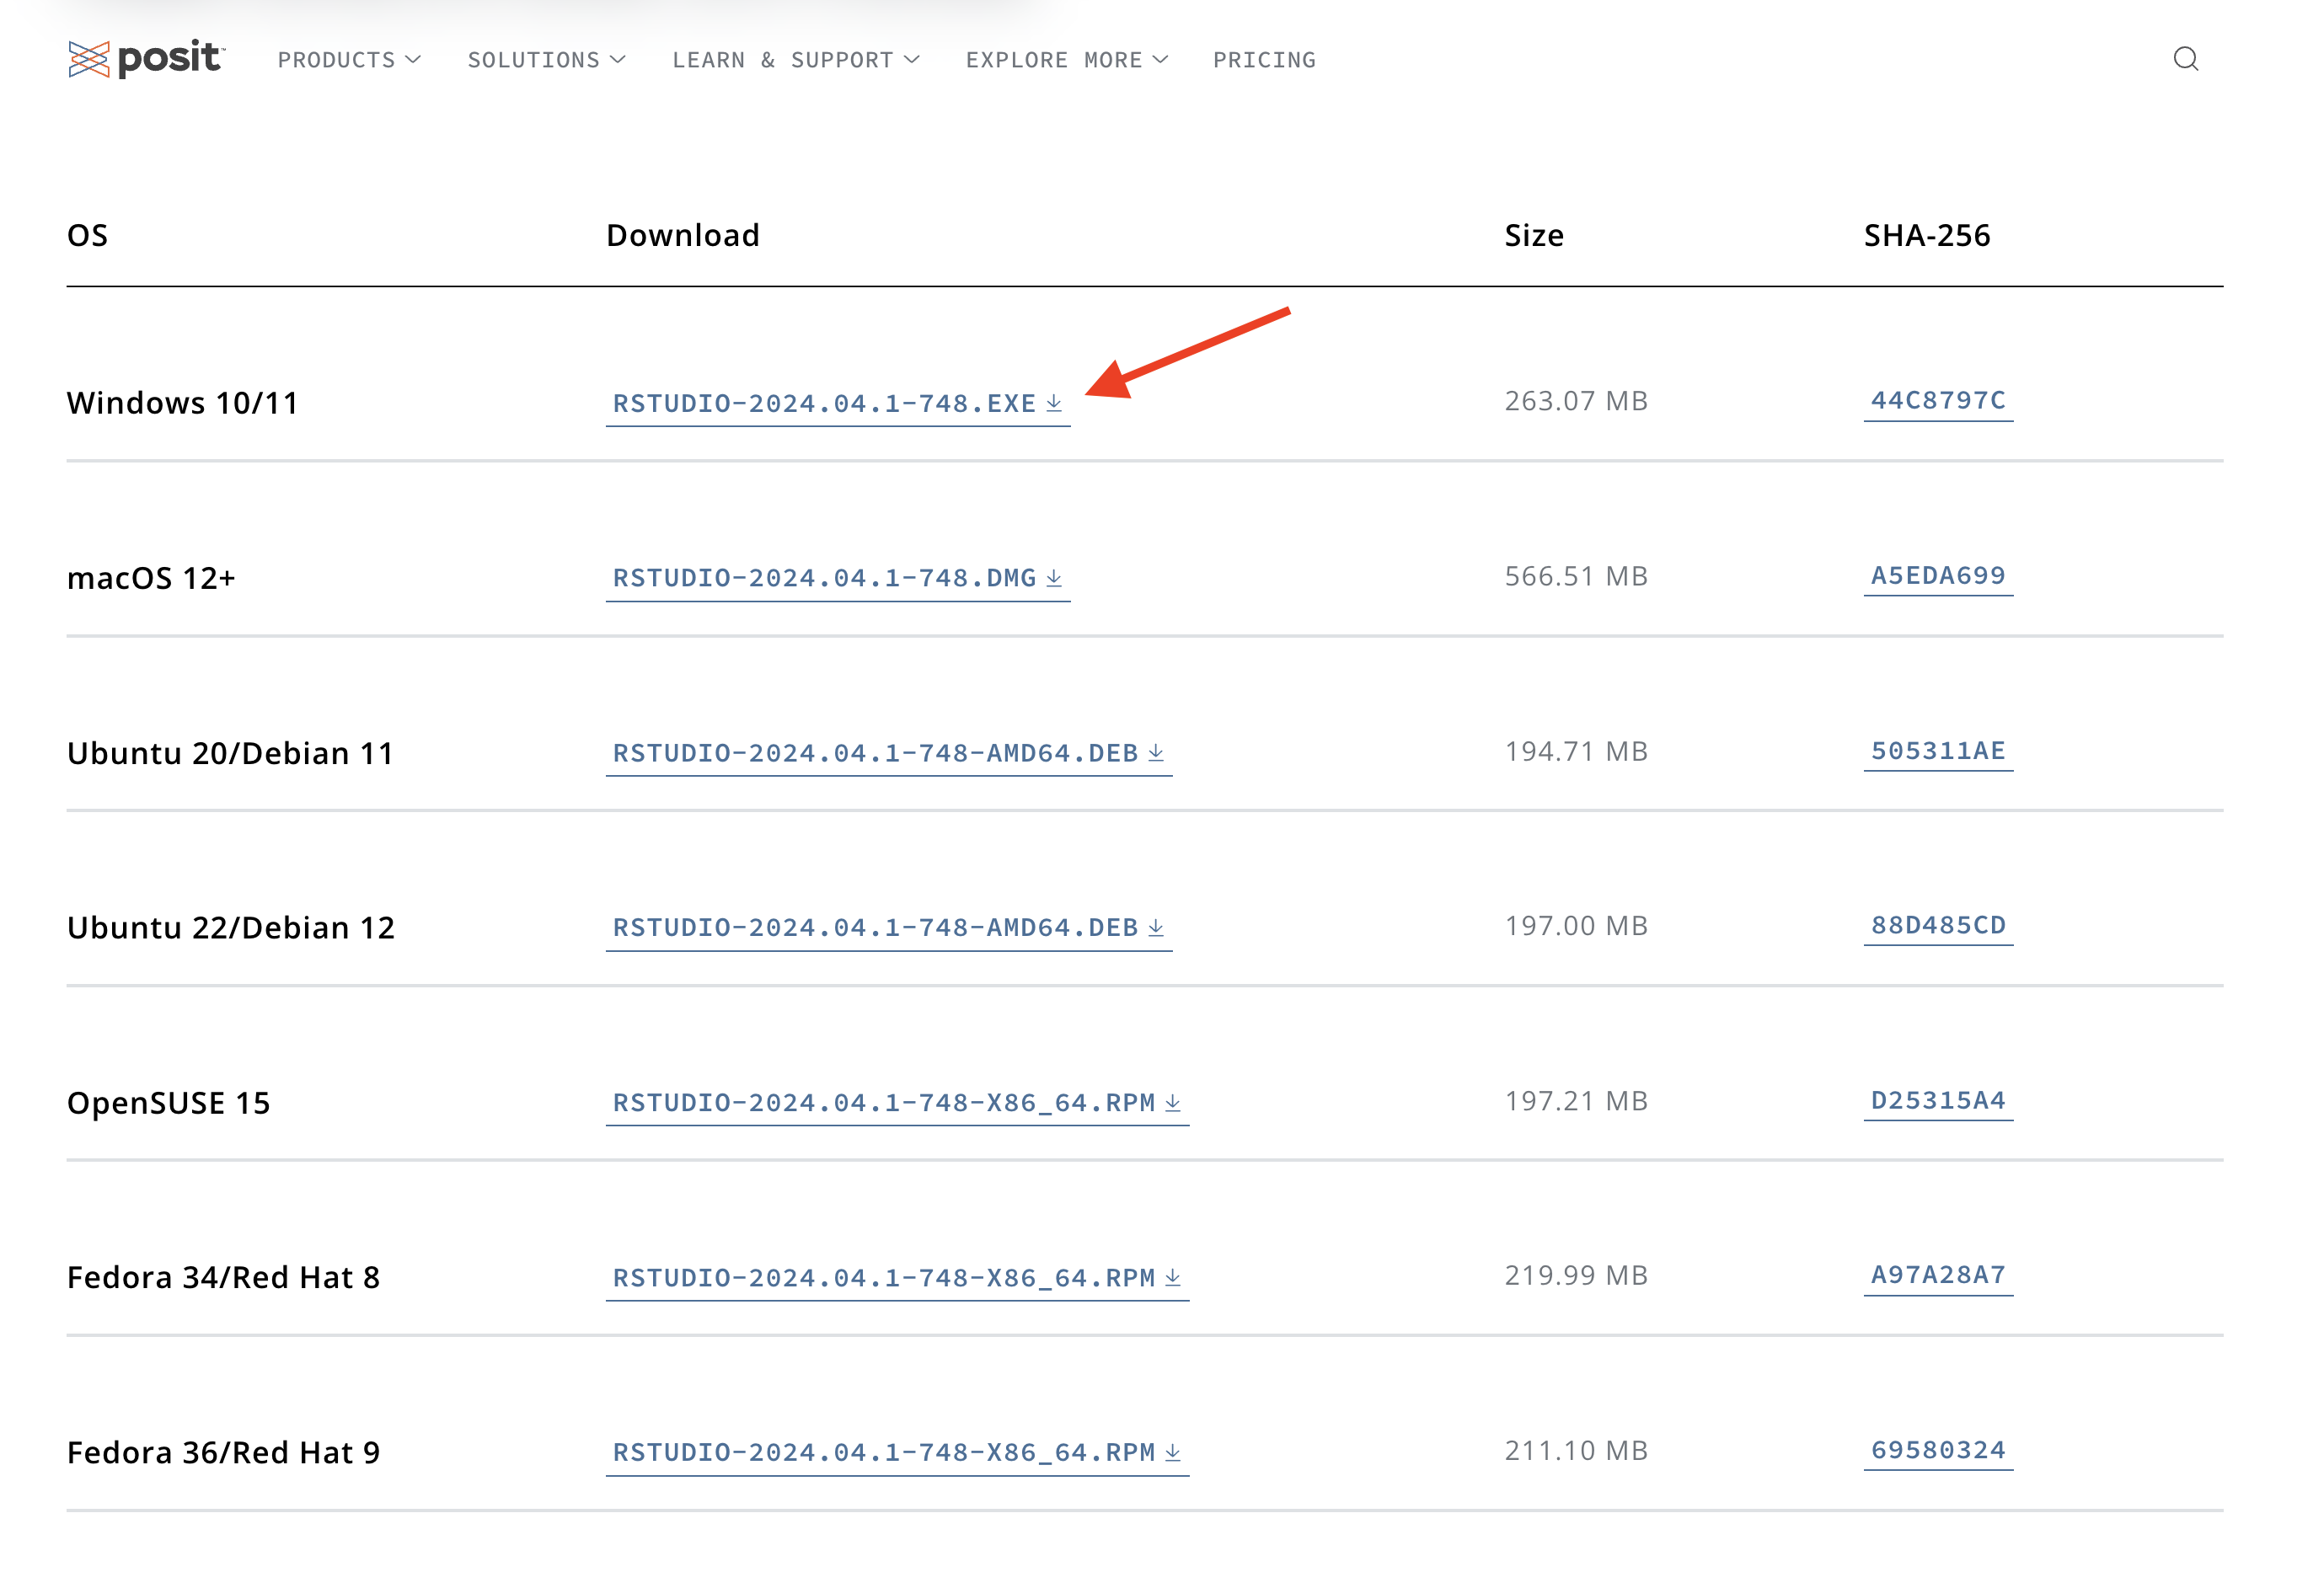
\includegraphics[keepaspectratio]{chapters/installing_r_and_rstudio/pc_download_rstudio1.png}}

\textbf{Step 9:} Again, locate the installation file you just downloaded
and double click it. Unless you've changed your download settings, this
file should be in the same location as the R installation file you
already downloaded.

\pandocbounded{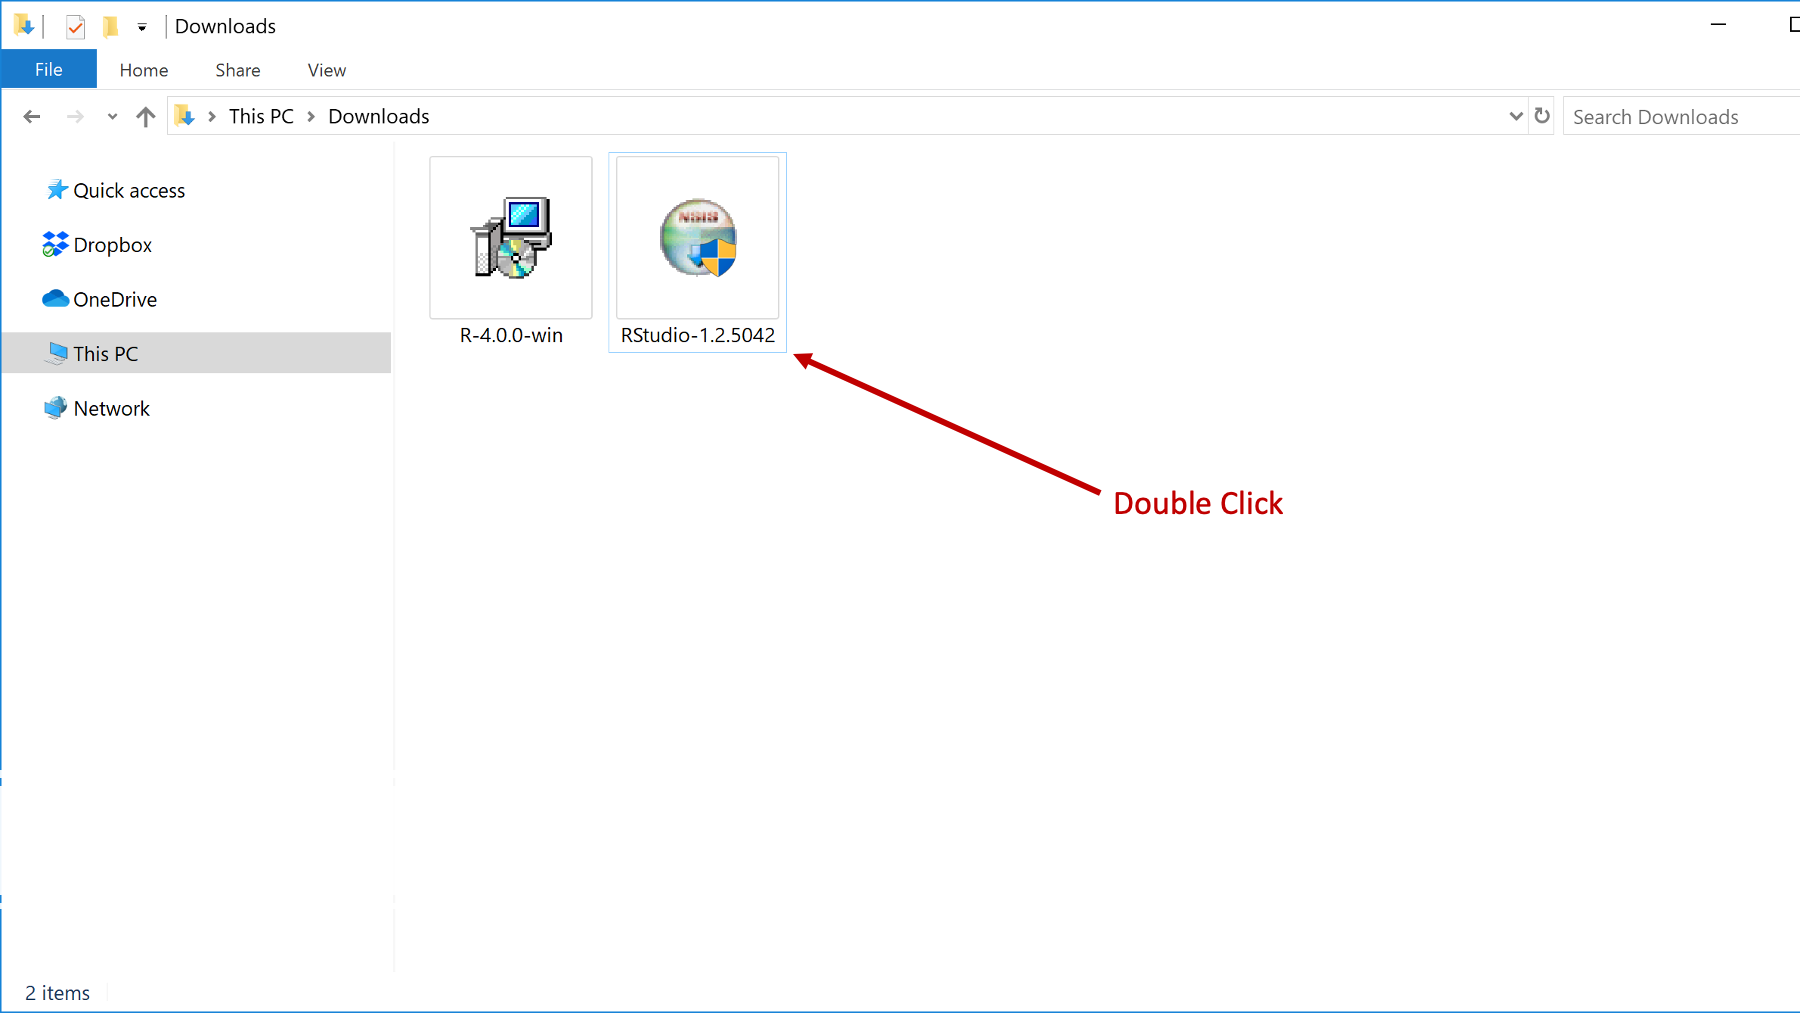
\includegraphics[keepaspectratio]{chapters/installing_r_and_rstudio/pc_install_rstudio1.png}}

\textbf{Step 10:} Another dialogue box will open and ask you to make
some decisions about how and where you want to install RStudio on your
computer. We typically just click ``Next'' at every step without
changing any of the default options.

\pandocbounded{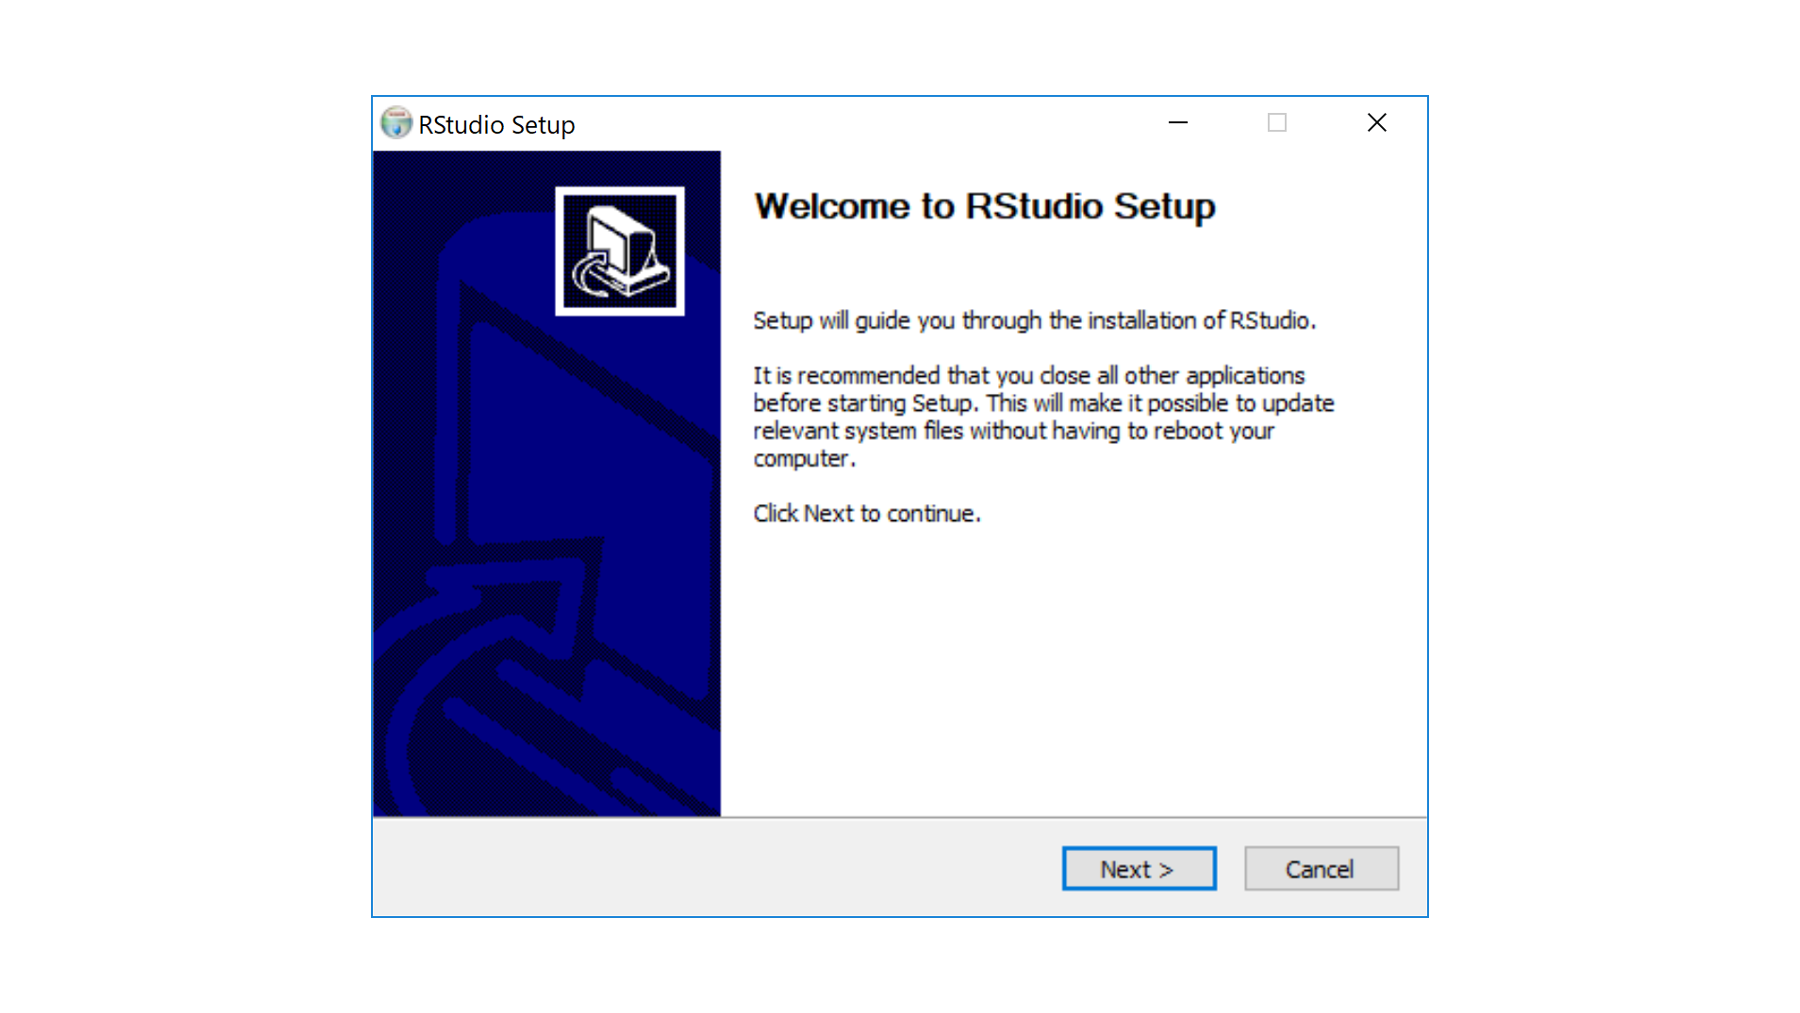
\includegraphics[keepaspectratio]{chapters/installing_r_and_rstudio/pc_install_rstudio2.png}}

When RStudio is finished installing, you should see RStudio in the
Windows start menu. Click the icon to open RStudio.

\pandocbounded{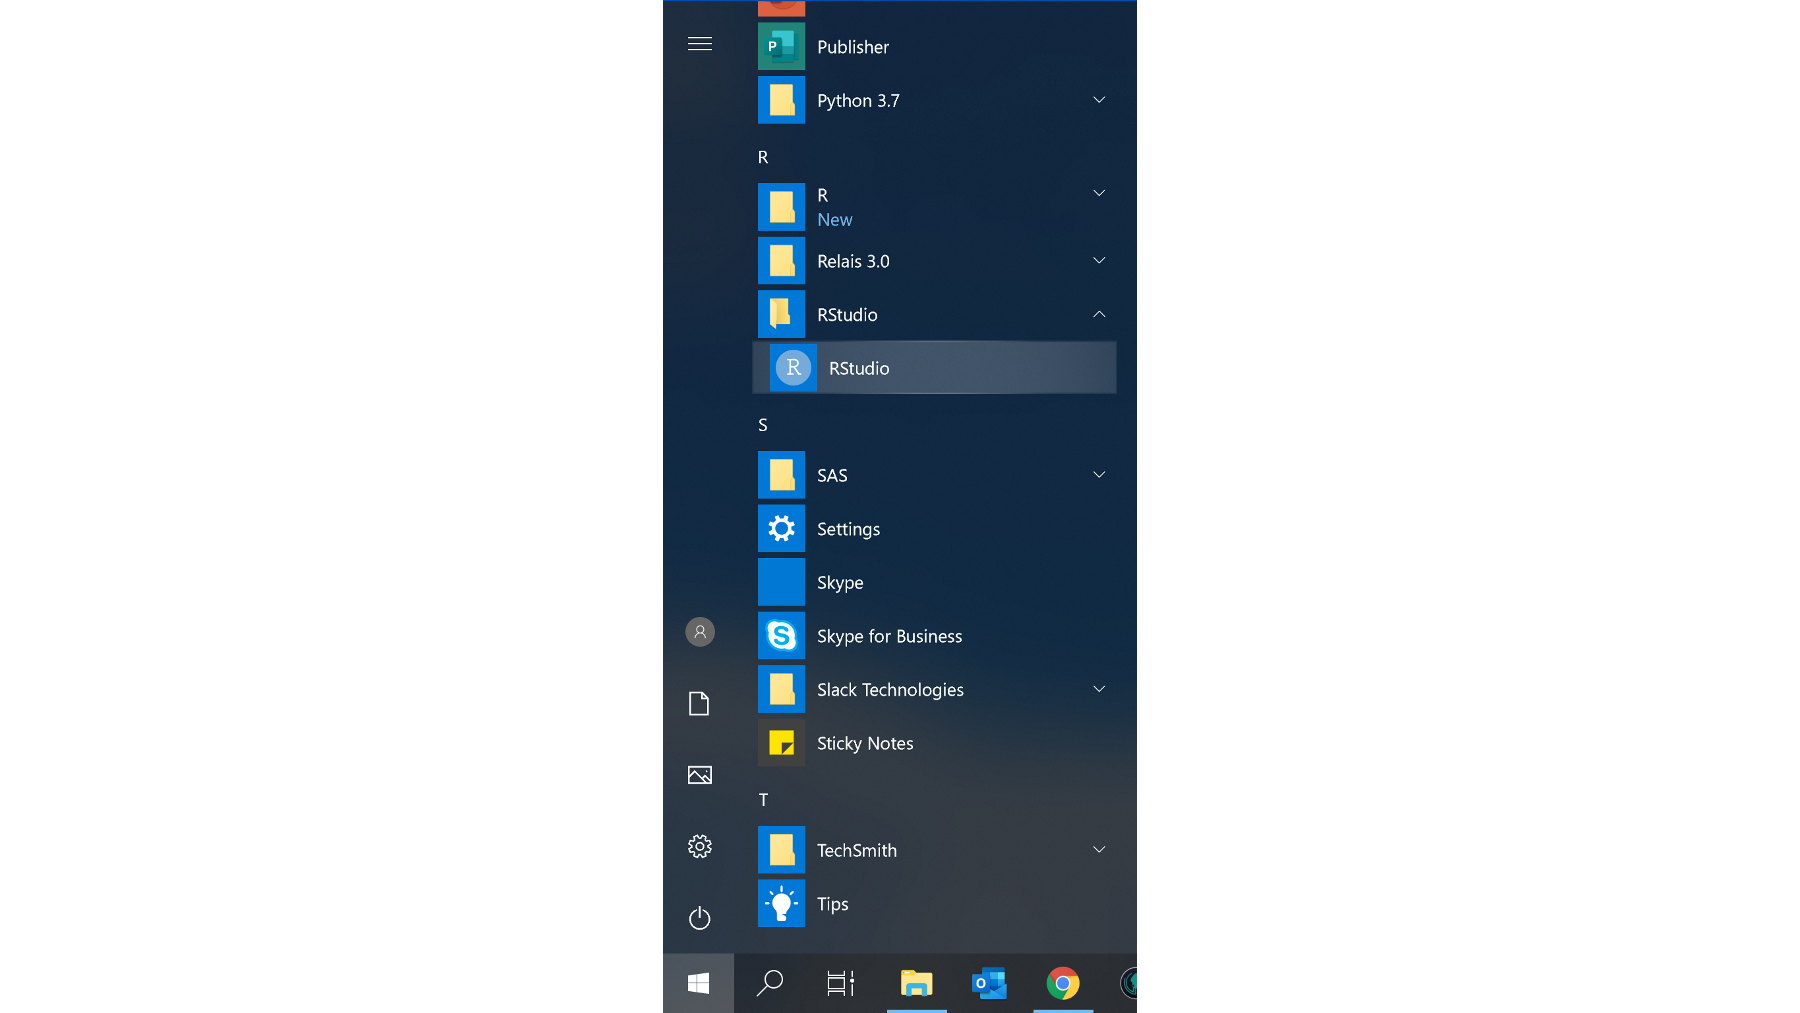
\includegraphics[keepaspectratio]{chapters/installing_r_and_rstudio/pc_view_rstudio1.png}}

The RStudio IDE should open and look something like the window you see
here. If so, you are good to go! 🎉

\pandocbounded{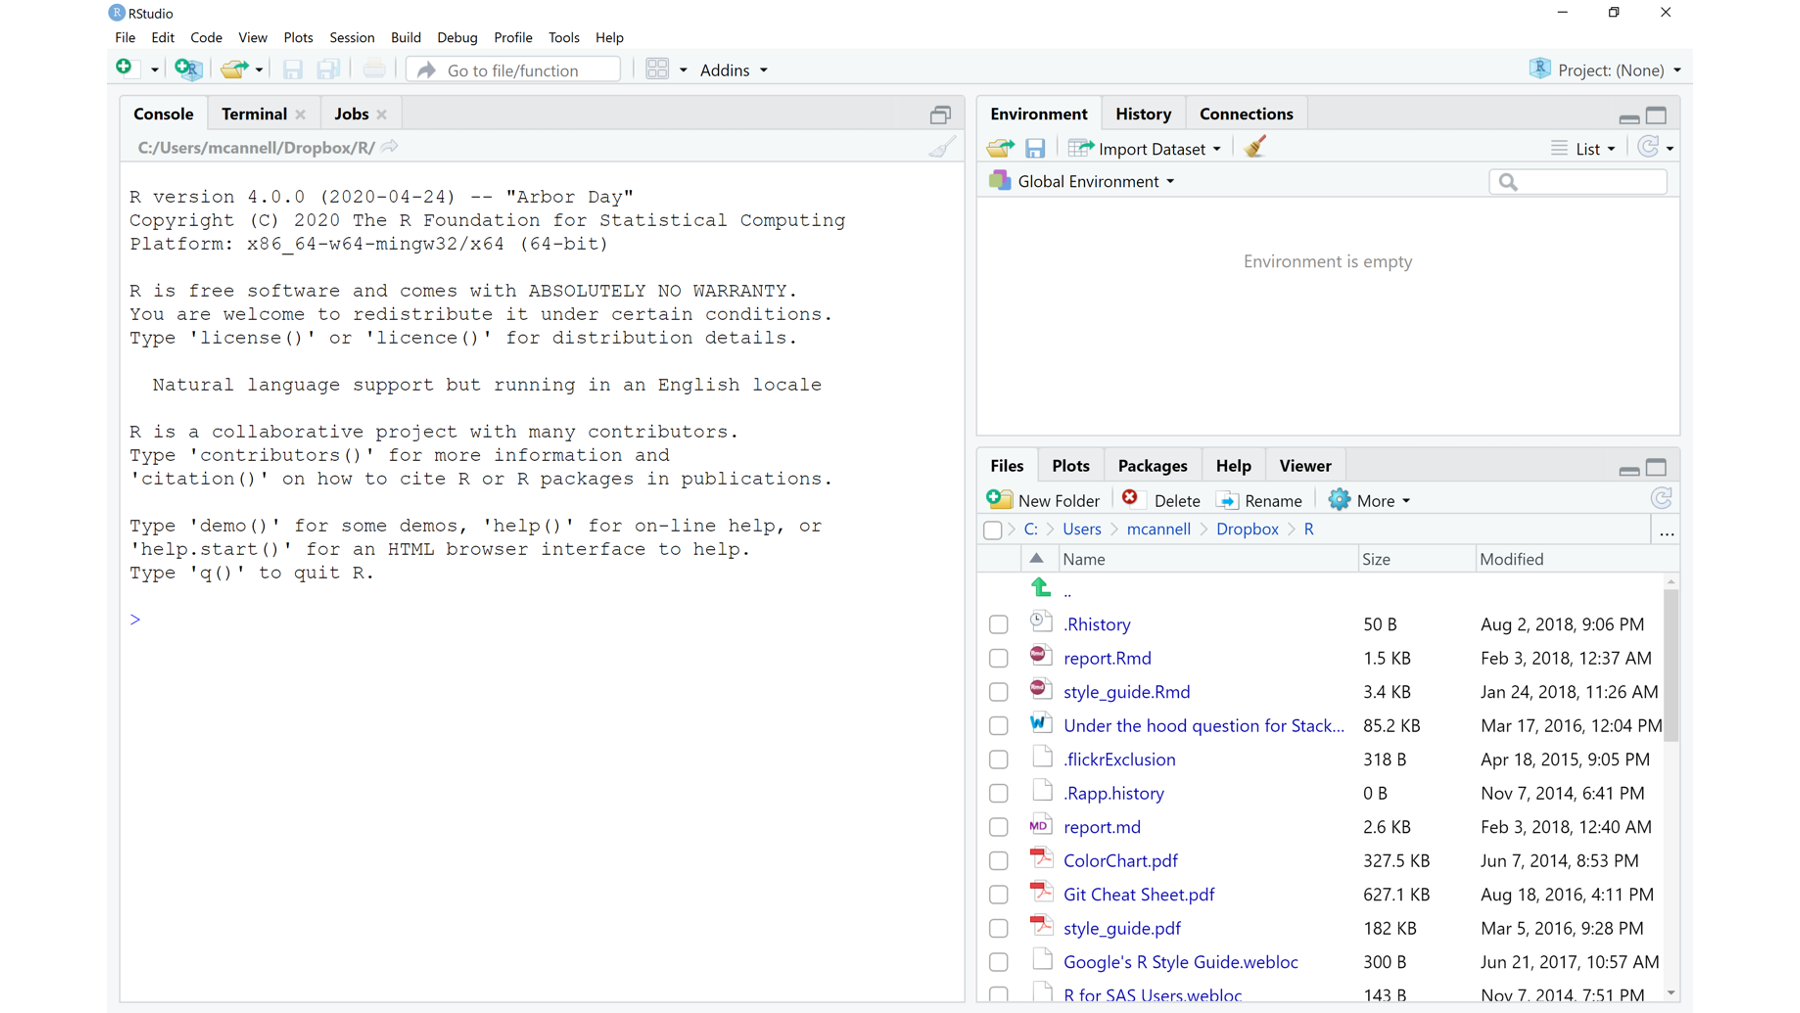
\includegraphics[keepaspectratio]{chapters/installing_r_and_rstudio/pc_view_rstudio2.png}}

\chapter{What is R?}\label{what-is-r}

At this point in the book, you should have installed R and RStudio on
your computer, but you may be thinking to yourself, ``I don't even know
what R is.'' Well, in this chapter you'll find out. We'll start with an
overview of the R language, and then briefly touch on its capabilities
and uses. You'll also see a complete R program and some complete
documents generated by R programs. In this book you'll learn how to
create similar programs and documents, and by the end of the book you'll
be able to write your own R programs and present your results in the
form of an issue brief written for general audiences who may or may not
have public health expertise. But, before we discuss R let's discuss
something even more basic -- data. Here's a question for you: What is
data?

\section{What is data?}\label{what-is-data}

Data is information about objects (e.g., people, places, schools) and
observable phenomenon (e.g., weather, temperatures, and disease
symptoms) that is recorded and stored somehow as a collection of
symbols, numbers, and letters. So, data is just information that has
been ``written'' down.

Here we have a table, which is a common way of organizing data. In R, we
will typically refer to these tables as \textbf{data frames}.

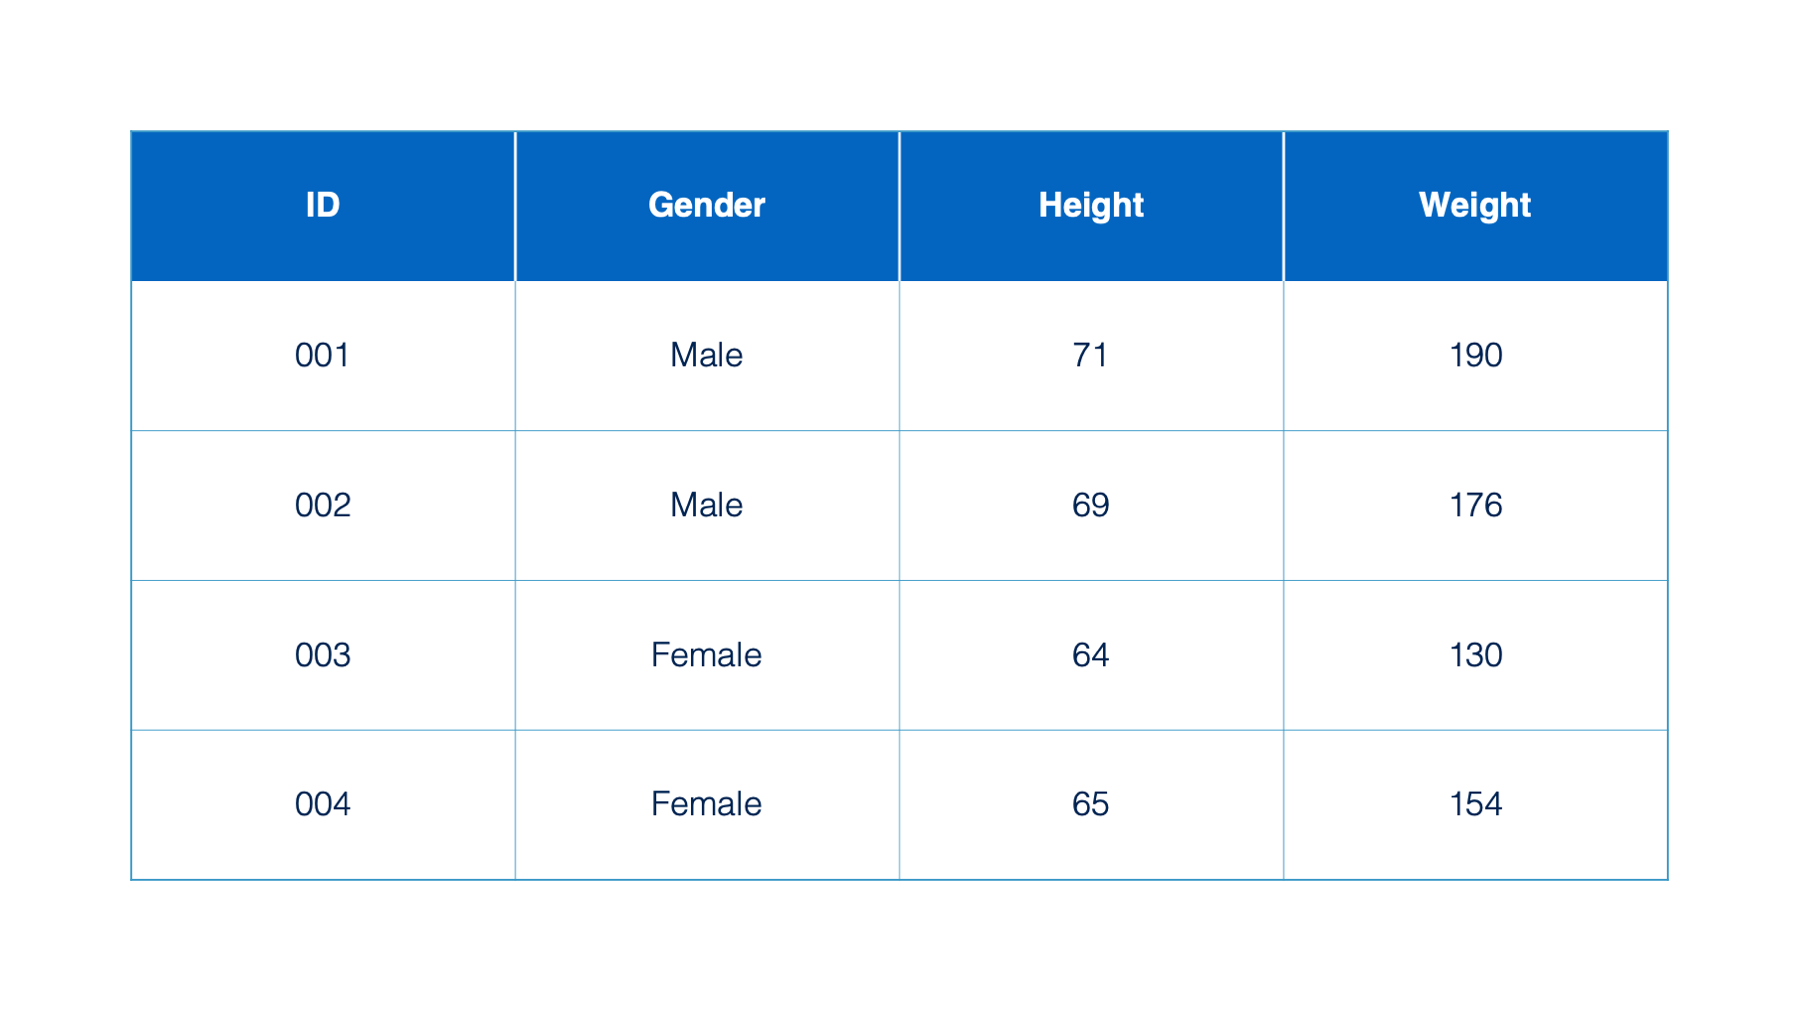
\includegraphics[width=6in,height=\textheight,keepaspectratio]{chapters/what_is_r/table.png}

Each box in a data frame is called a \textbf{cell}.

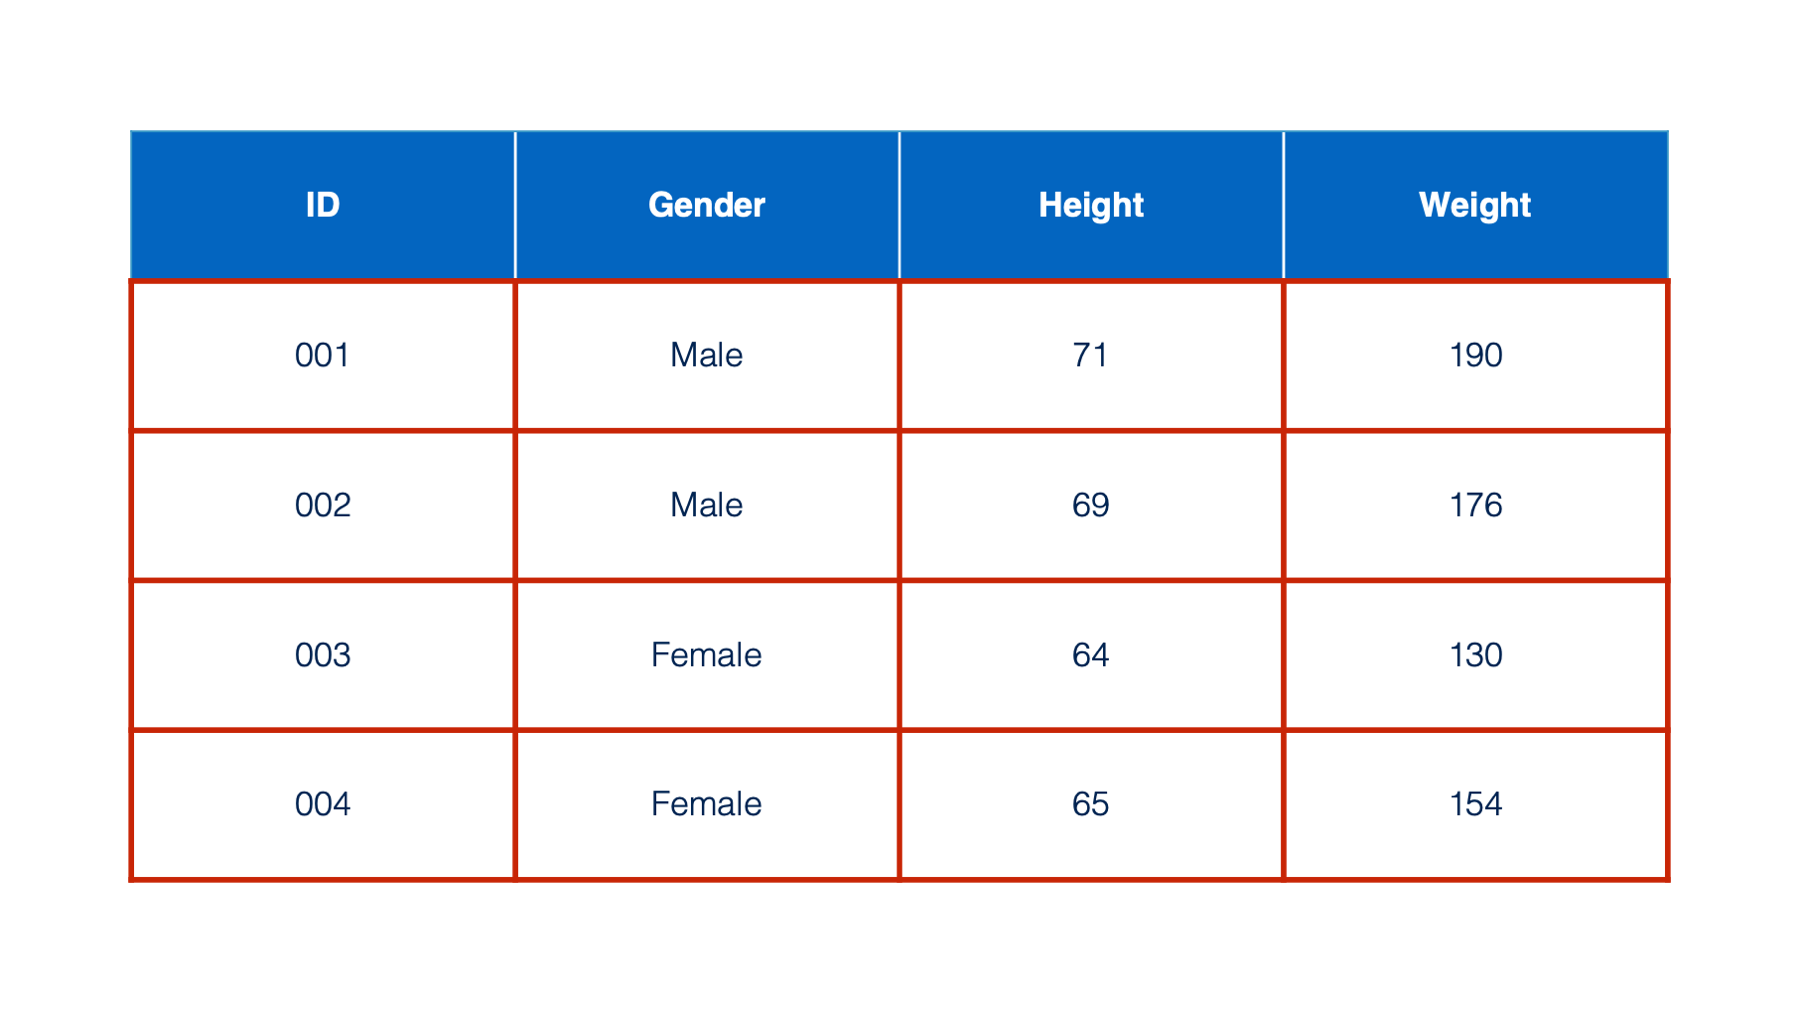
\includegraphics[width=6in,height=\textheight,keepaspectratio]{chapters/what_is_r/table_cells.png}

Moving from left to right across the data frame are \textbf{columns}.
Columns are also sometimes referred to as \textbf{variables}. In this
book, we will often use the terms columns and variables interchangeably.
Each column in a data frame has one, and only one, type. For now, know
that the type tells us what kind of data is contained in a column and
what we can \emph{do} with that data. You may have already noticed that
3 of the columns in the table we've been looking at contain numbers and
1 of the columns contains words. These columns will have different types
in R and we can do different things with them based on their type. For
example, we could ask R to tell us what the average value of the numbers
in the height column are, but it wouldn't make sense to ask R to tell us
the average value of the words in the Gender column. We will talk more
about many of the different column types exist in R later in this book.

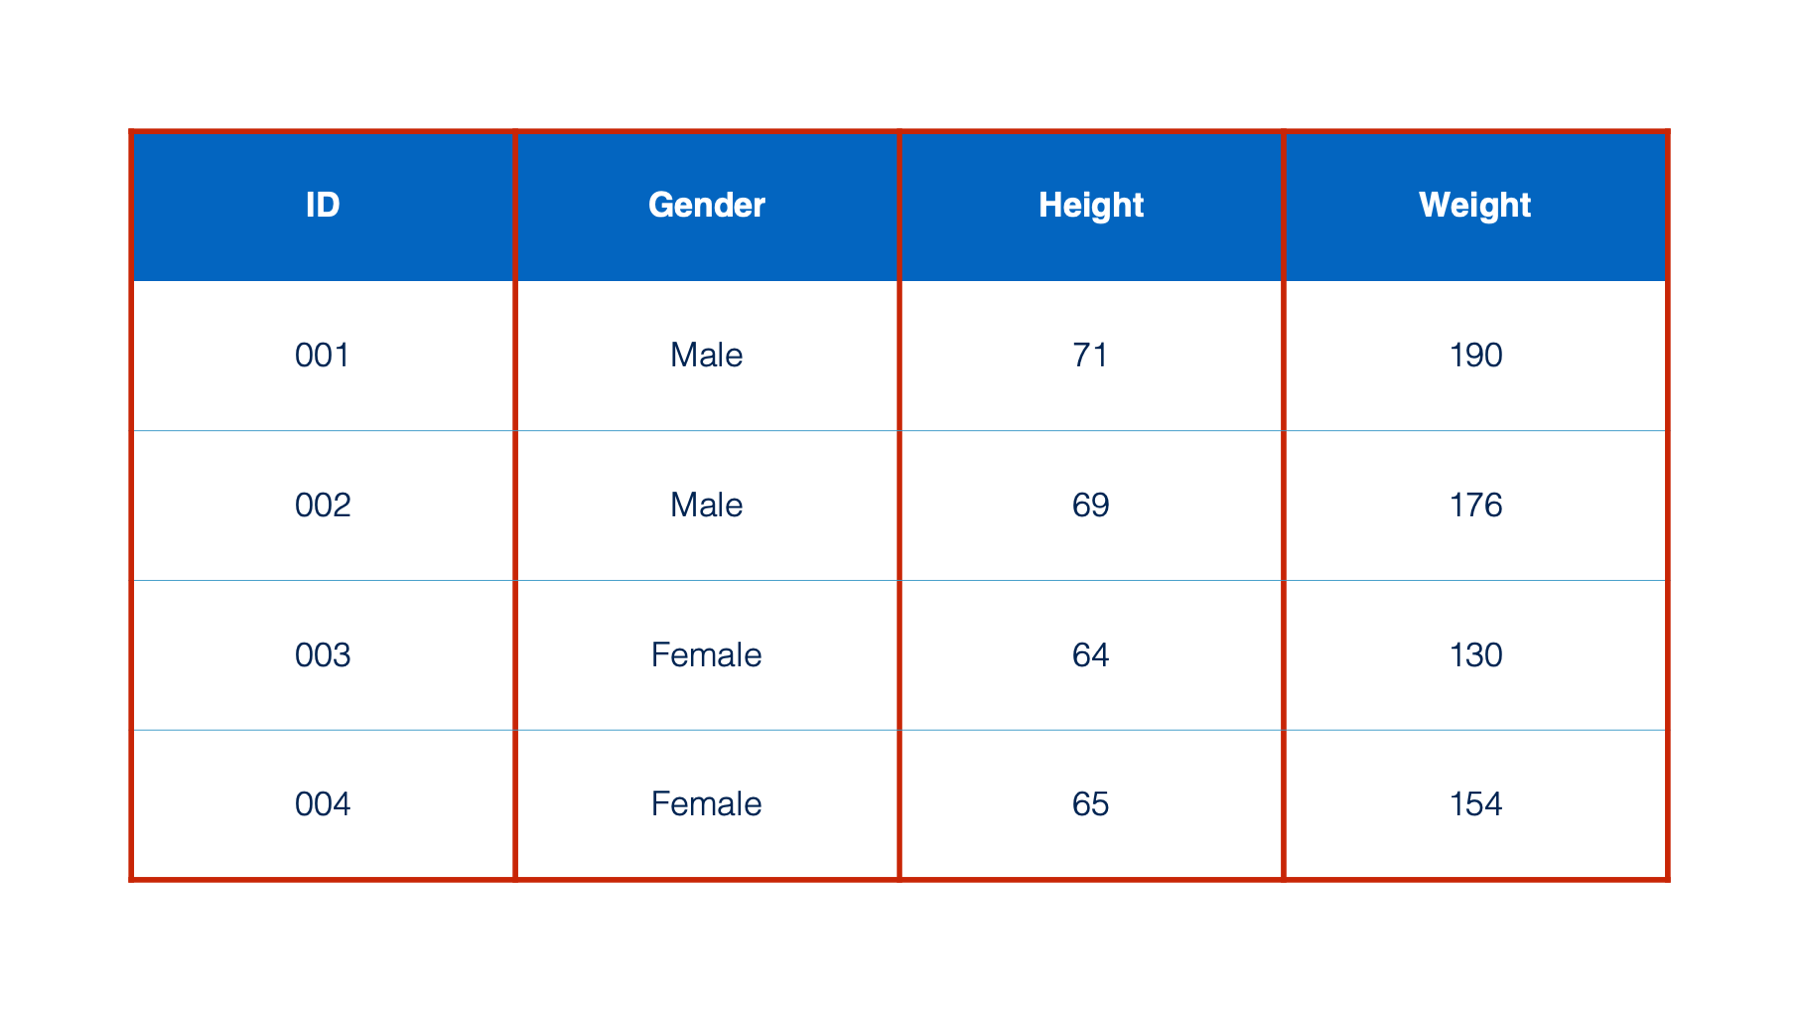
\includegraphics[width=6in,height=\textheight,keepaspectratio]{chapters/what_is_r/table_columns.png}

The information contained in the first cell of each column is called the
\textbf{column name} (or variable) name.

R gives us a lot of flexibility in terms of what we can name our
columns, but there are a few rules.

\begin{enumerate}
\def\labelenumi{\arabic{enumi}.}
\tightlist
\item
  Column names can contain letters, numbers and the dot (.) or
  underscore (\_) characters.\\
\item
  Additionally, they can begin with a letter or a dot -- as long as the
  dot is not followed by a number. So, a name like ``.2cats'' is not
  allowed.\\
\item
  Finally, R has some reserved words that you are not allowed to use for
  column names. These include: ``if'', ``else'', ``repeat'', ``while'',
  ``function'', ``for'', ``in'', ``next'', and ``break''.
\end{enumerate}

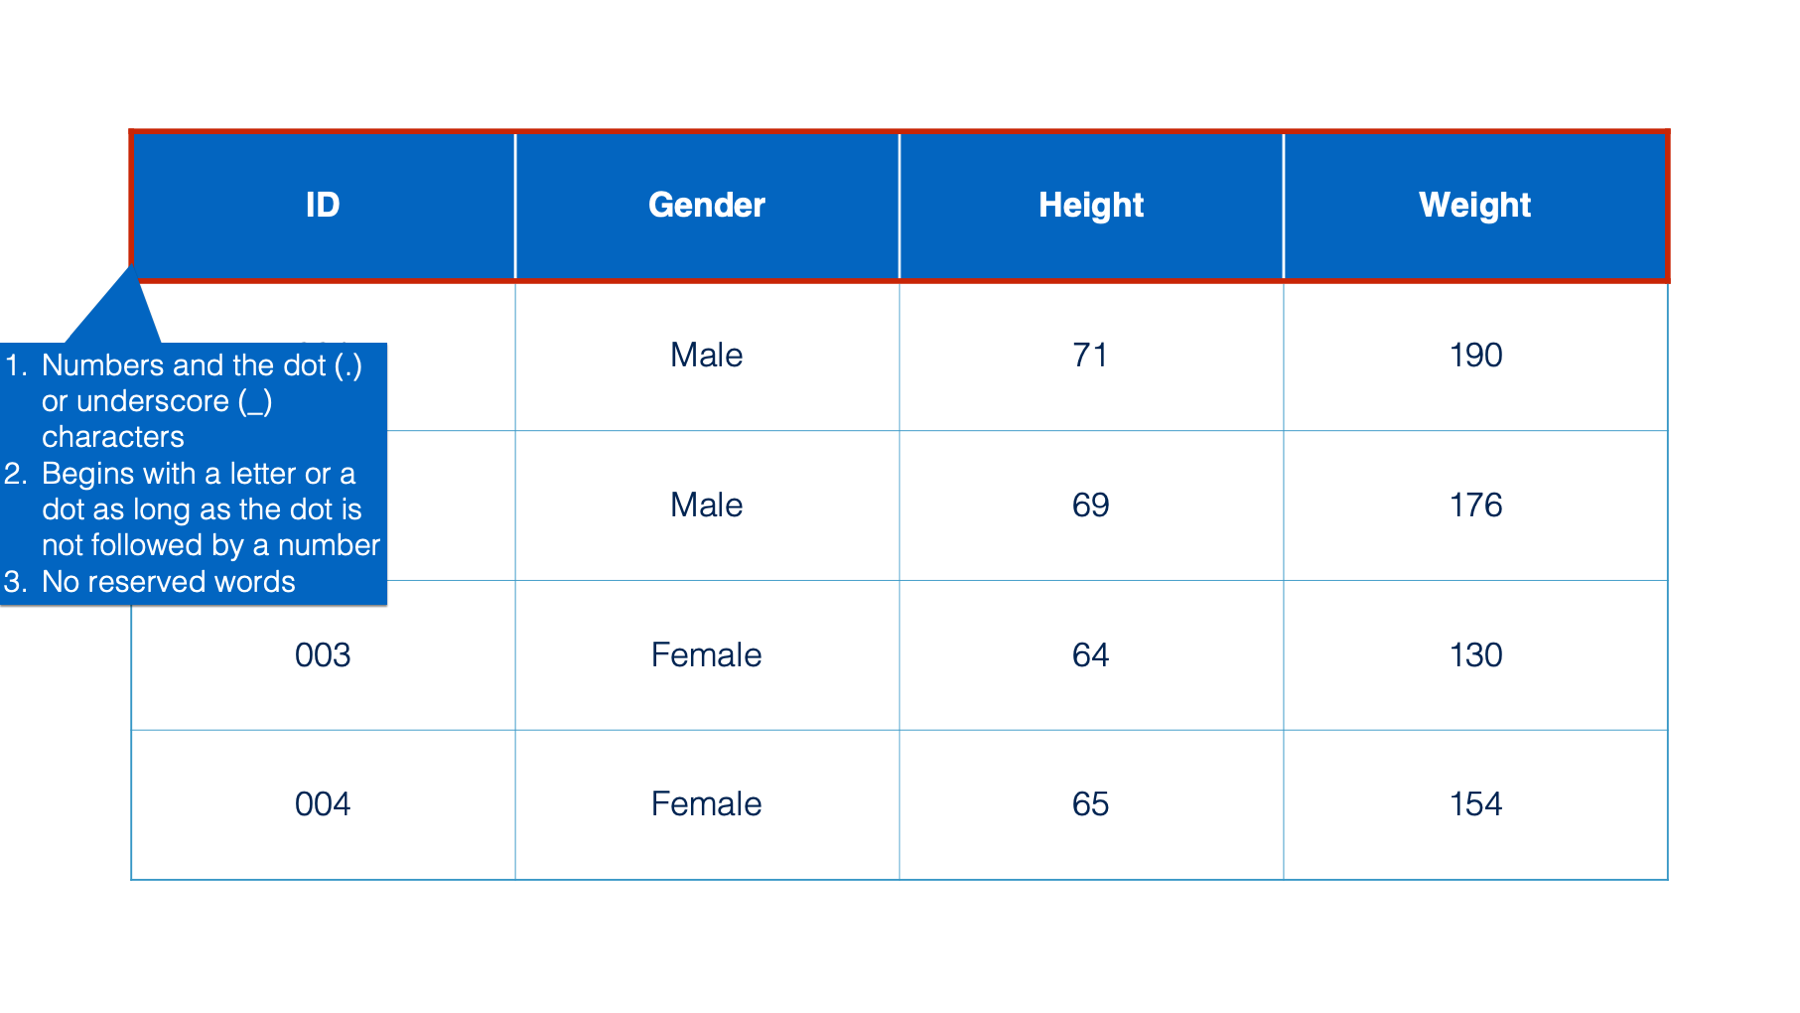
\includegraphics[width=6in,height=\textheight,keepaspectratio]{chapters/what_is_r/table_column_name.png}

Moving from top to bottom across the table are \textbf{rows}, which are
sometimes referred to as records.

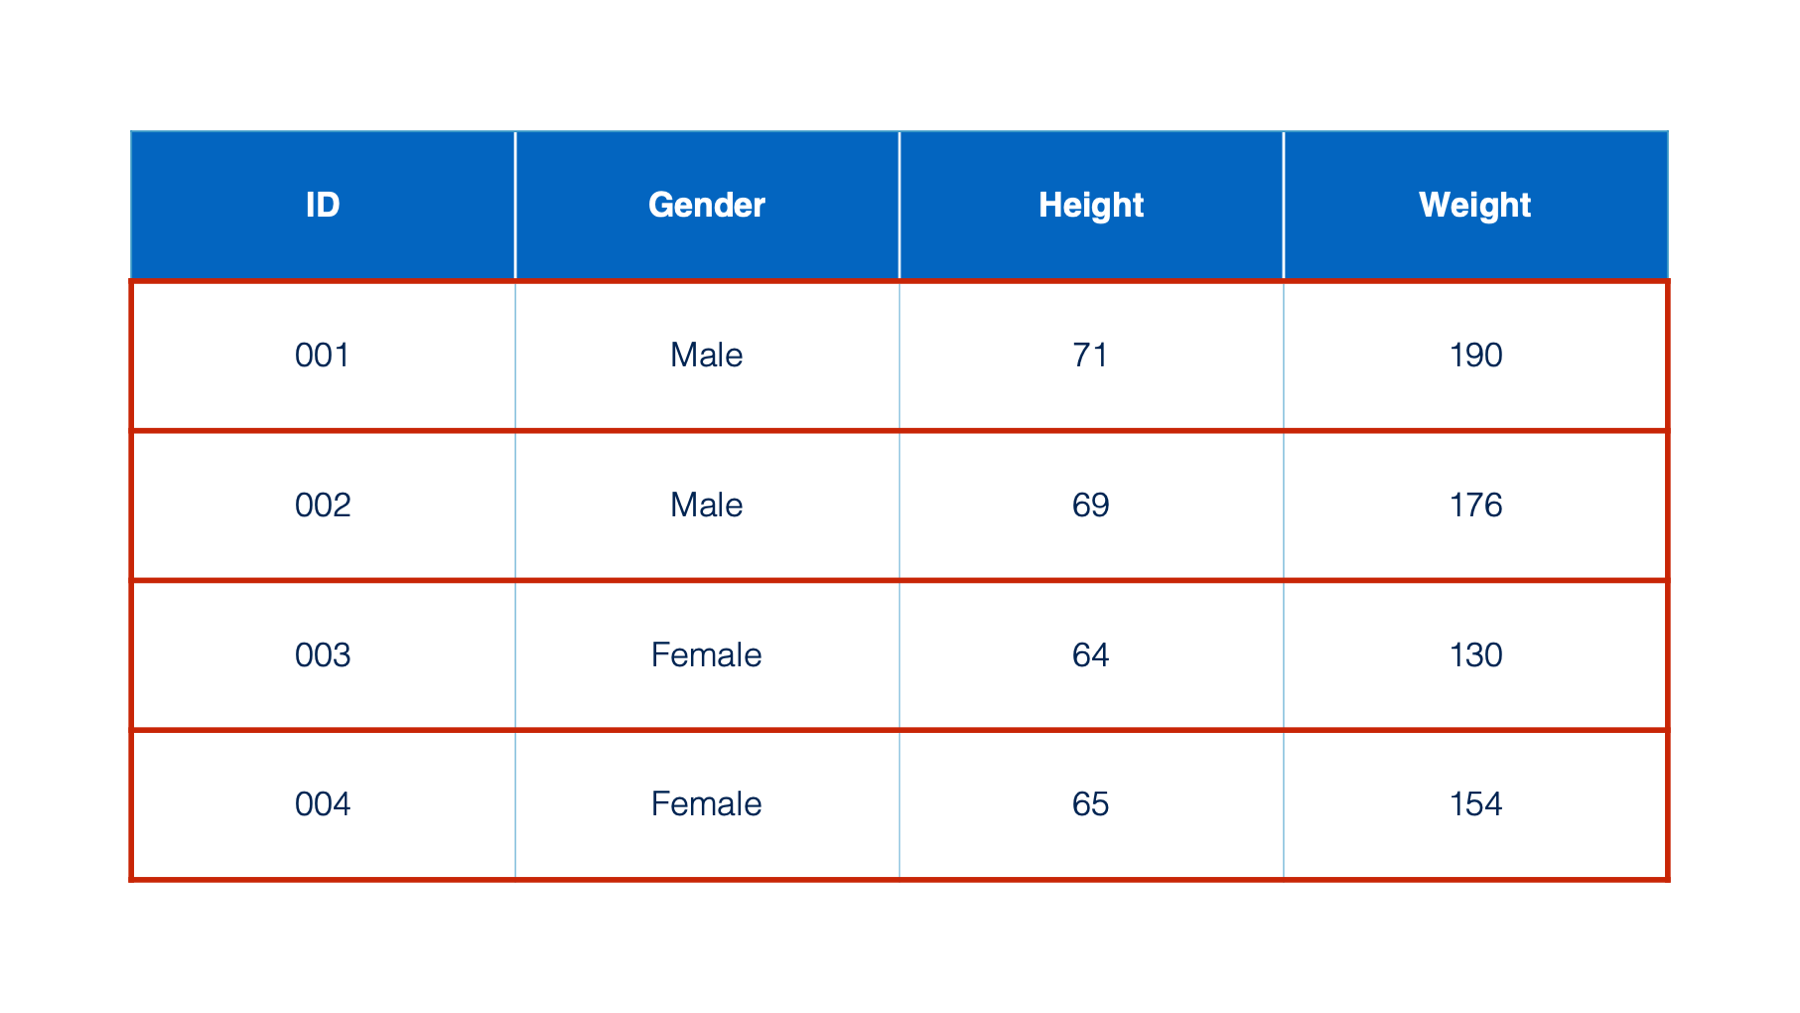
\includegraphics[width=6in,height=\textheight,keepaspectratio]{chapters/what_is_r/table_rows.png}

Finally, the contents of each cell are called \textbf{values}.

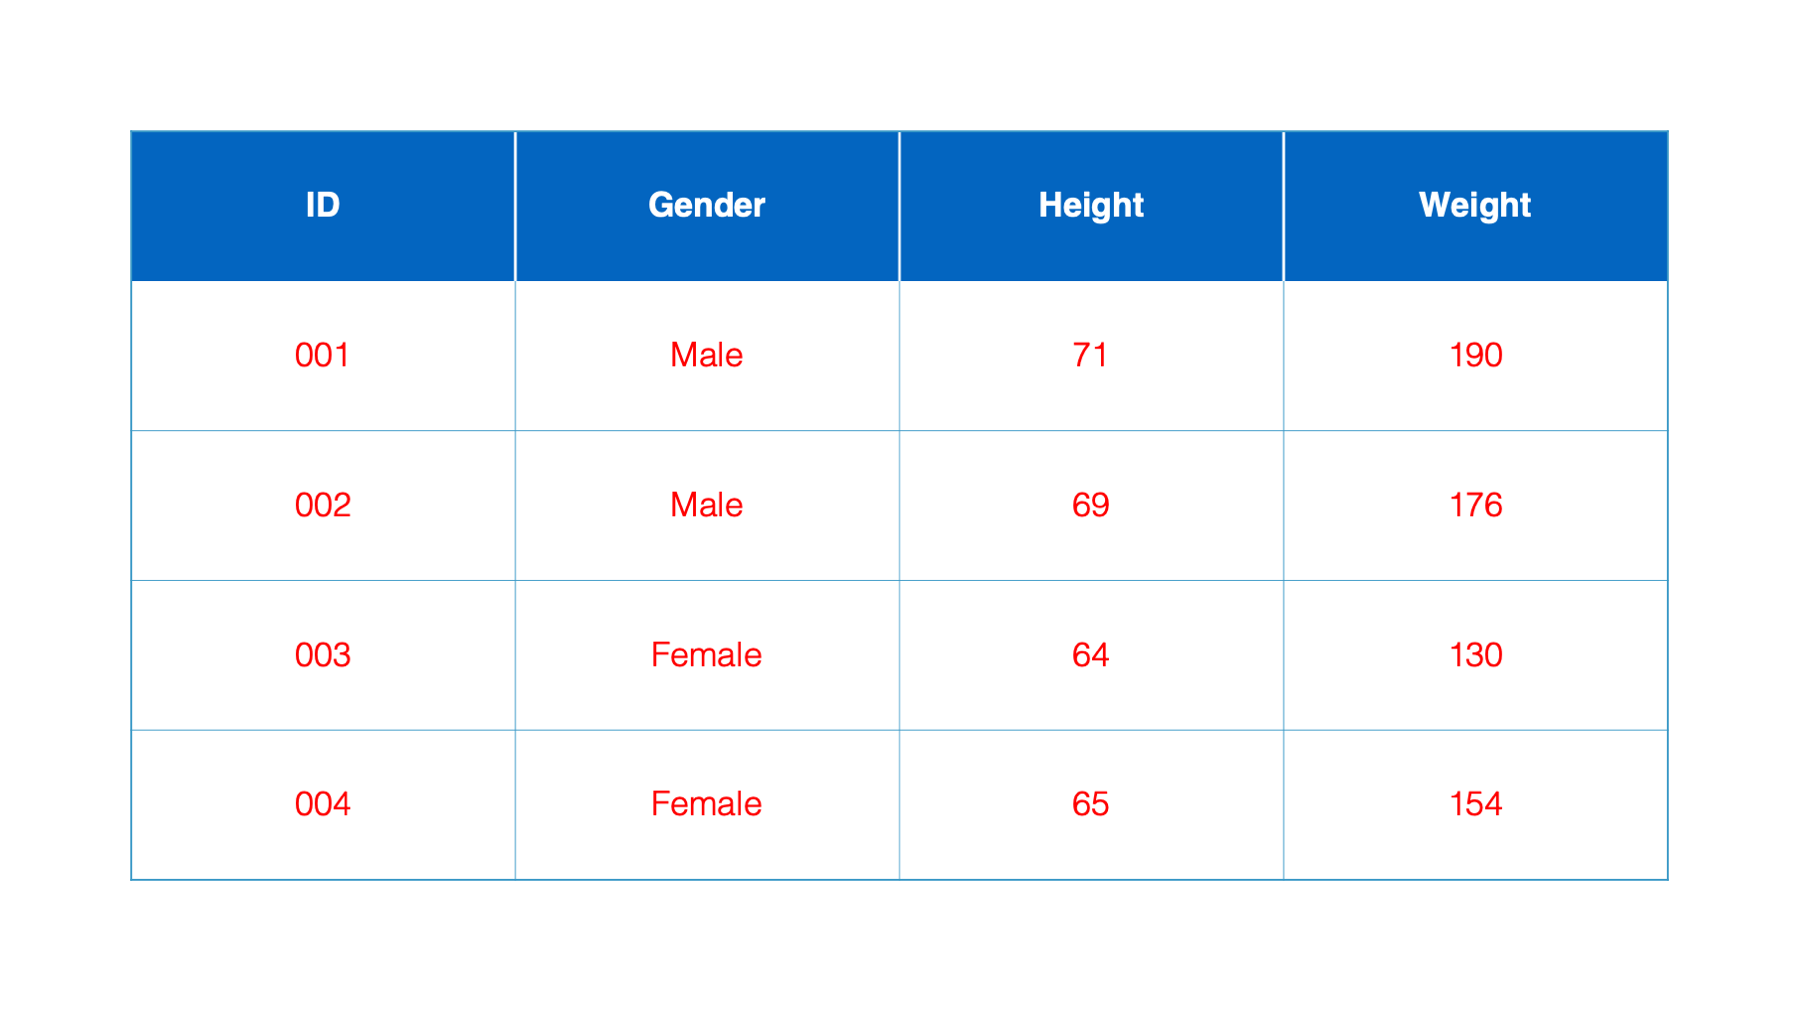
\includegraphics[width=6in,height=\textheight,keepaspectratio]{chapters/what_is_r/table_values.png}

We should now be up to speed on some basic terminology used by R, as
well as other analytic, database, and spreadsheet programs. These terms
will be used repeatedly throughout the book.

\section{What is R?}\label{what-is-r-1}


\includegraphics[width=6in,height=\textheight,keepaspectratio]{chapters/what_is_r/r_logo.png}

So, what is R? Well, R is an \textbf{open source} statistical
programming language that was created in the 1990's specifically for
data analysis. We will talk more about what open source means later, but
for now, just think of R as an easy (relatively 😂) way to ask our
computer to do math and statistics for us. More specifically, by the end
of this book we will be able to independently use R to transfer data,
manage data, analyze data, and present the results of our analysis.
Let's quickly take a closer look at each of these.

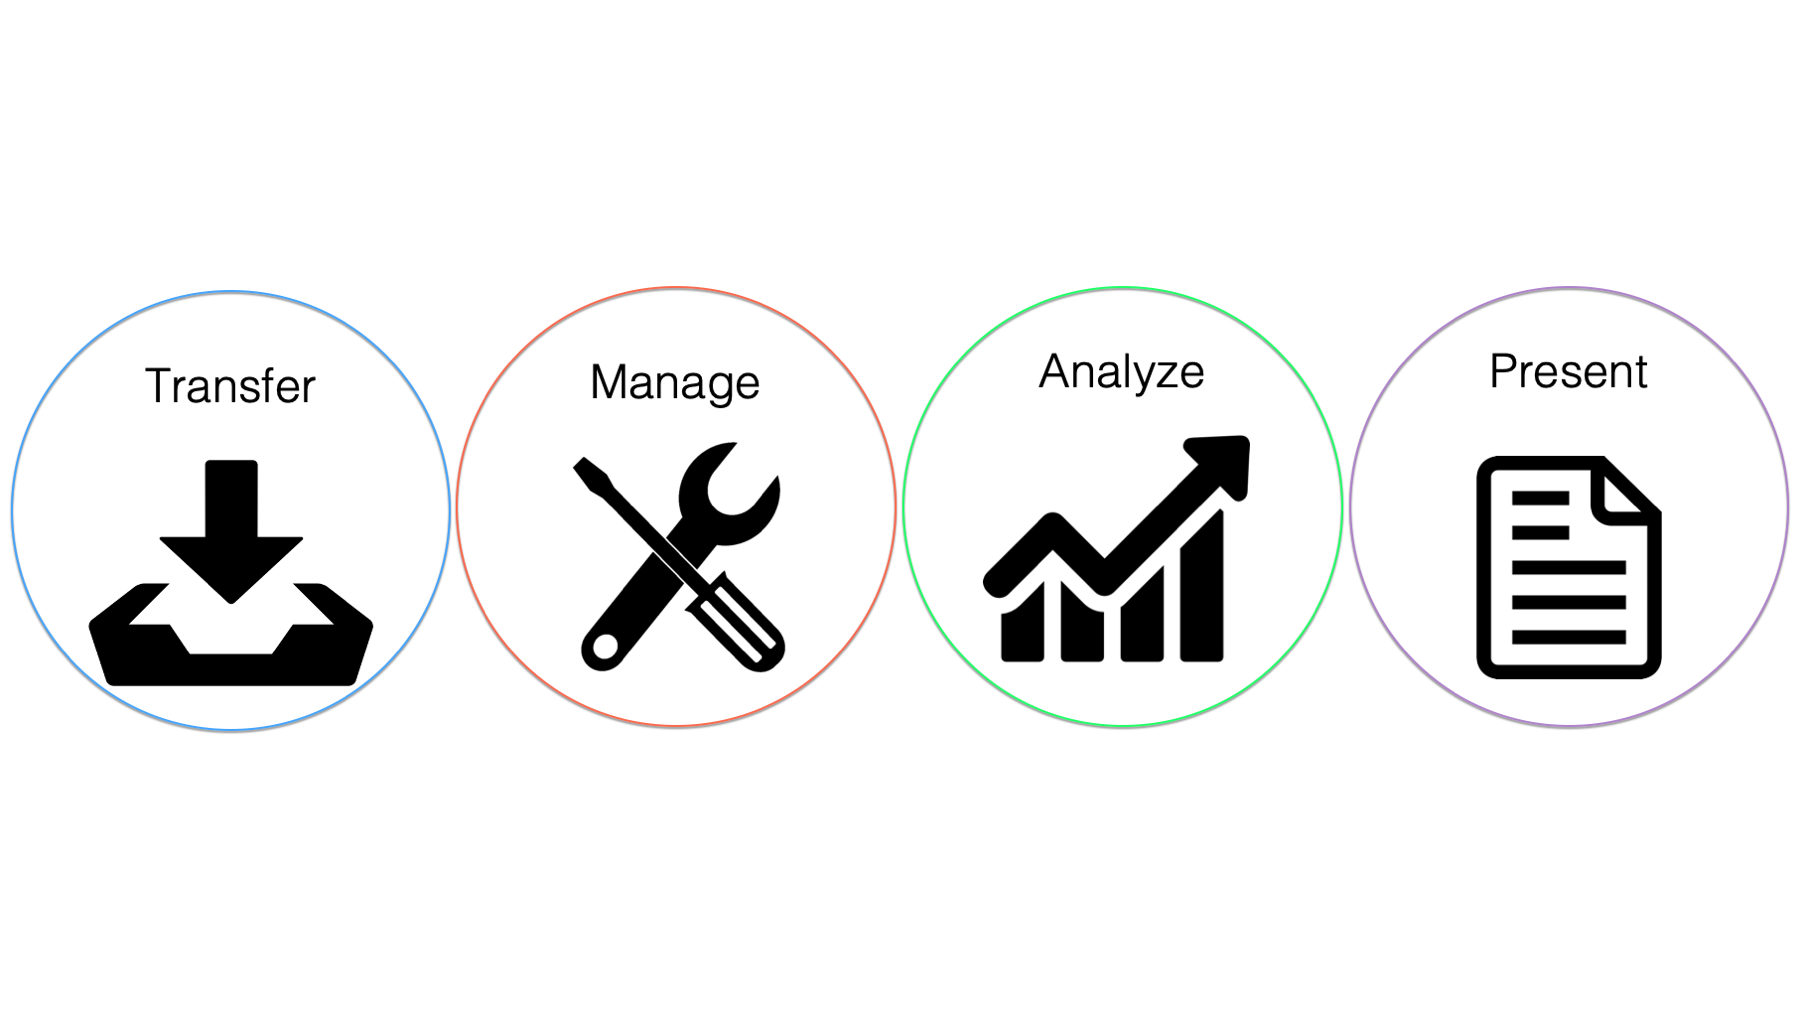
\includegraphics[width=6in,height=\textheight,keepaspectratio]{chapters/what_is_r/competencies_overview.png}

\subsection{Transferring data}\label{transferring-data}

\includegraphics[width=6in,height=\textheight,keepaspectratio]{chapters/what_is_r/competencies_transfer.png}

So, what do we mean by ``transfer data''? Well, individuals and
organizations store their data using different computer programs that
use different file types. Some common examples that we may come across
in epidemiology are database files, spreadsheets, raw data files, and
SAS data sets. No matter how the data is stored, we can't do anything
with it until we can get it into R, in a form that R can use, and in a
location that R can access.

\subsection{Managing data}\label{managing-data}

\includegraphics[width=6in,height=\textheight,keepaspectratio]{chapters/what_is_r/competencies_manage.png}

This isn't very specific, but managing data is all the things we may
have to do to our data to get it ready for analysis. Some people also
refer to this process as ``data wrangling'' or ``data munging.'' Some
specific examples of data management tasks include:

\begin{itemize}
\tightlist
\item
  \ul{Validating and cleaning data}. In other words, dealing with
  potential errors in the data.\\
\item
  \ul{Subsetting data} -- using only some of the columns or some of the
  rows.\\
\item
  \ul{Creating new variables}. For example, we might want to create a
  new \texttt{BMI} variable from existing \texttt{height} and
  \texttt{weight} variables.\\
\item
  \ul{Combining data frames}. For example, we might want to combine a
  data frame containing sociodemographic data about study participants
  with a data frame containing intervention outcomes data about those
  same participants.
\end{itemize}

We may sometimes hear people refer to the 80/20 rule about data
management. This ``rule'' says that in a typical data analysis project,
roughly 80\% of our time will be spent on data management, while only
20\% will be spent on the analysis itself. We can't provide you with any
empirical evidence (i.e., data) to back this claim up. But as people who
have been involved in many projects that involve the collection and
analysis of data, we can tell you anecdotally that this ''rule'' is
probably pretty close to being accurate in most cases.

Additionally, it's been our experience that most students of
epidemiology are required to take one or more courses that emphasize
methods for analyzing data; however, almost none of them have taken a
course that emphasizes data management.

Therefore, because data management is such a large component of most
projects that involve the collection and analysis of data, and because
most readers will have already been exposed to data analysis to a much
greater extent than data management, this book will start by heavily
emphasizing the latter.

\subsection{Analyzing data}\label{analyzing-data}

\includegraphics[width=6in,height=\textheight,keepaspectratio]{chapters/what_is_r/competencies_analysis.png}

As discussed above, this is probably the capability most people most
closely associate with R, and there is no doubt that R is a powerful
tool for analyzing data. However, in this book we won't go beyond using
R to calculate basic descriptive statistics. For our purposes,
descriptive statistics include:

\begin{itemize}
\tightlist
\item
  \ul{Measures of central tendency}. For example, mean, median, and
  mode.\\
\item
  \ul{Measures of dispersion}. For example, variance and standard
  error.\\
\item
  \ul{Measures for describing categorical variables}. For example,
  counts and percentages.\\
\item
  \ul{Describing data using graphs and charts}. With R, we can describe
  our data using \href{https://www.r-graph-gallery.com/}{beautiful and
  informative graphs}.
\end{itemize}

\subsection{Presenting data}\label{presenting-data}

\includegraphics[width=6in,height=\textheight,keepaspectratio]{chapters/what_is_r/competencies_present.png}

And finally, the ultimate goal is typically to present our findings in
some form or another. For example, a report, a website, or a journal
article. With R we can present our results in many different formats
with relative ease. In fact, this is one of our favorite things about R
and RStudio. In this book we will learn how to publish our text,
tabular, or graphical results in many different formats including
Microsoft Word documents, html files that can be viewed in web browsers,
and pdf documents. Let's take a look at some examples.

\begin{enumerate}
\def\labelenumi{\arabic{enumi}.}
\tightlist
\item
  \textbf{Microsoft Word documents}.
  \href{https://www.dropbox.com/s/6l1ikp6wbyue9bd/chap_2_example_word_docI.docx?dl=0}{Click
  here} to view an example report created for a research project in
  Microsoft Word.\\
\item
  \textbf{PDF documents}.
  \href{https://www.dropbox.com/s/hheuyv5qcabf197/chap_2_example_pdf.pdf?dl=0}{Click
  here} to view a data dictionary created in PDF format.\\
\item
  \textbf{HTML files}. Hypertext Markup Language (HTML) files are what
  we are looking at whenever we view a webpage. We can use R to create
  HTML files that others can view in their web browser. We can email
  them these files to view in their web browser, or we can make them
  available for others to view online just like any other website.
  \href{https://rstudio.github.io/flexdashboard/articles/examples.html}{Click
  here} to view an gallery of data dashboards created with R.\\
\item
  \textbf{Web applications}. We can even use R to create full-fledged
  web applications. View the
  \href{https://shiny.rstudio.com/gallery/}{RStudio website} to see some
  examples.
\end{enumerate}

\chapter{Navigating the RStudio
Interface}\label{navigating-the-rstudio-interface}

If you followed along with the previous chapters, you have R and RStudio
installed on your computer and you have some idea of what R and RStudio
are. At this point, it can be common for people to open RStudio and get
totally overwhelmed. \emph{``What am I looking at?''} \emph{''What do I
click first?''} \emph{``Where do I even start?''} Don't worry if these,
or similar, thoughts have crossed your mind. You are in good company and
we will start to clear some of them up in this chapter.

When we load RStudio, we should see a screen that looks very similar to
Figure~\ref{fig-rstudio} below. There, we see three \textbf{panes}, and
each pane has multiple tabs.

\begin{figure}

\centering{

\includegraphics[width=10.07in,height=\textheight,keepaspectratio]{chapters/navigating_rstudio/rstudio.png}

}

\caption{\label{fig-rstudio}The default RStudio user interface.}

\end{figure}%

\section{The console pane}\label{the-console-pane}

The first pane we are going to talk about is the
\textbf{console/terminal/background jobs} pane.

\begin{figure}

\centering{

\includegraphics[width=10.07in,height=\textheight,keepaspectratio]{chapters/navigating_rstudio/console.png}

}

\caption{\label{fig-console}The R Console.}

\end{figure}%

It's called the ``console/terminal/background jobs'' pane because it has
three tabs we can click on by default: ``console'', ``terminal'', and
``background jobs''. However, we will refer to this pane as the
``console pane'' and will mostly ignore the terminal and background jobs
tabs for now. We aren't ignoring them because they aren't useful;
instead, we are ignoring them because using them isn't essential for
anything we will discuss in this chapter, and we want to keep things as
simple as possible for now.

The \hyperref[glossary-console]{console} is the most basic way to
interact with R. We can type a command to R into the console prompt (the
prompt looks like ``\textgreater{}'') and R will respond to what we
type. For example, below we typed ``1 + 1,'' pressed the return/enter
key, and the R console returned the sum of the numbers 1 and 1.

\begin{figure}

\centering{

\includegraphics[width=10.07in,height=\textheight,keepaspectratio]{chapters/navigating_rstudio/one_plus_one.png}

}

\caption{\label{fig-one-plus-one}Doing some addition in the R console.}

\end{figure}%

The number 1 we see in brackets before the 2 (i.e., {[}1{]}) is telling
us that this line of results starts with the first result. That fact is
obvious here because there is only one result. So, let's look at a
result that spans multiple lines to make this idea clearer.

\begin{figure}

\centering{

\includegraphics[width=10.07in,height=\textheight,keepaspectratio]{chapters/navigating_rstudio/seq_function.png}

}

\caption{\label{fig-seq-function}Demonstrating a function that returns
multiple results.}

\end{figure}%

In Figure~\ref{fig-seq-function} we see examples of a couple of new
concepts that are worth discussing.

First, as promised, we have more than one line of results (or output).
The first line of results starts with a 1 in brackets (i.e., {[}1{]}),
which indicates that this line of results starts with the first result.
In this case, the first result is the number 2. The second line of
results starts with a 29 in brackets (i.e., {[}29{]}), which indicates
that this line of results starts with the twenty-ninth result. In this
case, the twenty-ninth result is the number 58. If we count the numbers
in the first line, there should be 28 -- results 1 through 28. We also
want to make it clear that ``1'' and ``29'' are \emph{NOT} results
themselves. They are just helping us count the number of results per
line.

The second new thing that you may have noticed in
Figure~\ref{fig-seq-function} is our use of a \textbf{function}.
Functions are a \textbf{BIG DEAL} in R. So much so that R is called a
\emph{functional language}. We don't really need to know all the details
of what that means; however, we should know that, in general, everything
we \emph{do} in R we will \emph{do} with a function. By contrast,
everything we \emph{create} in R will be an \emph{object}. If we wanted
to make an analogy between the R language and the English language, we
could think of functions as verbs -- they \emph{do} things -- and
objects as nouns -- they \emph{are} things. This distinction likely
seems abstract and confusing at the moment, but we will make it more
concrete soon.

Most functions in R begin with the function name followed by
parentheses. For example, \texttt{seq()}, \texttt{sum()}, and
\texttt{mean()}.

\emph{Question}: What is the name of the function we used in the example
above?

\emph{Answer}: We used the \texttt{seq()} function -- short for sequence
- in the example above.

You may notice that there are three pairs of words, equal symbols, and
numbers that are separated by commas inside the \texttt{seq()} function.
They are, \texttt{from\ =\ 2}, \texttt{to\ =\ 100}, and
\texttt{by\ =\ 2}. The words \texttt{from}, \texttt{to}, and \texttt{by}
are all \hyperref[glossary-arguments]{arguments} to the \texttt{seq()}
function. We will learn more about functions and arguments later. For
now, just know that arguments \emph{give functions the information they
need to give us the result we want}.

In this case, the \texttt{seq()} function
\hyperref[glossary-returns]{returns} a sequence of numbers. But first,
we had to give it information about where that sequence should start,
where it should end, and how many steps should be in the middle. Above,
the sequence began with the value we \hyperref[glossary-pass]{passed} to
the \texttt{from} argument (i.e., 2), it ended with the value we passed
to the \texttt{to} argument (i.e., 100), and it increased at each step
by the number we passed to the \texttt{by} argument (i.e., 2). So, 2, 4,
6, 8 \ldots{} 100.

Whether you realize it or not, we've covered some important programming
terms while discussing the \texttt{seq()} function above. Before we move
on to discussing RStudio's other panes, let's quickly review and
reinforce a few of terms we will use repeatedly in this book.

\begin{itemize}
\item
  \hyperref[glossary-arguments]{Arguments}: Arguments always live
  \emph{inside} the parentheses of R functions and receive information
  the function needs to generate the result we want.
\item
  \hyperref[glossary-pass]{Pass}: In programming lingo, we \emph{pass} a
  value to a function argument. For example, in the function call
  \texttt{seq(from\ =\ 2,\ to\ =\ 100,\ by\ =\ 2)} we could say that we
  \emph{passed} a value of 2 to the \texttt{from} argument, we
  \emph{passed} a value of 100 to the \texttt{to} argument, and we
  \emph{passed} a value of 2 to the \texttt{by} argument.
\item
  \hyperref[glossary-return]{Return}: Instead of saying, ``the
  \texttt{seq()} function \emph{gives us} a sequence of
  numbers\ldots{}'' we say, ``the \texttt{seq()} function \emph{returns}
  a sequence of numbers\ldots{}'' In programming lingo, functions
  \emph{return} one or more results.
\end{itemize}

\begin{tcolorbox}[enhanced jigsaw, toptitle=1mm, breakable, colback=white, toprule=.15mm, leftrule=.75mm, arc=.35mm, opacityback=0, coltitle=black, left=2mm, bottomrule=.15mm, bottomtitle=1mm, opacitybacktitle=0.6, title=\textcolor{quarto-callout-note-color}{\faInfo}\hspace{0.5em}{Note}, colframe=quarto-callout-note-color-frame, titlerule=0mm, rightrule=.15mm, colbacktitle=quarto-callout-note-color!10!white]

🗒\textbf{Side Note:} The \texttt{seq()} function isn't particularly
important or noteworthy. We essentially chose it at random to illustrate
some key points. However, arguments, passing values, and return values
are extremely important concepts and we will return to them many times.

\end{tcolorbox}

\section{The environment pane}\label{the-environment-pane}

The second pane we are going to talk about is the
environment/history/connections pane in
Figure~\ref{fig-environment-pane}. However, we will mostly refer to it
as the environment pane and we will mostly ignore the history and
connections tab. We aren't ignoring them because they aren't useful;
rather, we are ignoring them because using them isn't essential for
anything we will discuss anytime soon, and we want to keep things as
simple as possible.

\begin{figure}

\centering{

\includegraphics[width=10.07in,height=\textheight,keepaspectratio]{chapters/navigating_rstudio/environment_pane.png}

}

\caption{\label{fig-environment-pane}The environment pane}

\end{figure}%

The Environment pane shows you all the \textbf{objects} that R can
currently use for data management or analysis. In this picture,
Figure~\ref{fig-environment-pane} our environment is empty. Let's create
an object and add it to our environment.

\begin{figure}

\centering{

\includegraphics[width=10.07in,height=\textheight,keepaspectratio]{chapters/navigating_rstudio/environment_pane2.png}

}

\caption{\label{fig-environment-pane2}The vector x in the global
environment.}

\end{figure}%

Here we see that we created a new object called \texttt{x}, which now
appears in our \textbf{Global Environment}.
Figure~\ref{fig-environment-pane2} This gives us another great
opportunity to discuss some new concepts.

First, we created the \texttt{x} object in the console by
\emph{assigning} the value 2 to the letter x. We did this by typing
``x'' followed by a less than symbol (\textless), a dash symbol (-), and
the number 2. R is kind of unique in this way. We have never seen
another programming language (although I'm sure they are out there) that
uses \texttt{\textless{}-} to assign values to variables. By the way,
\texttt{\textless{}-} is called the assignment operator (or assignment
arrow), and ''assign'' here means ``make x contain 2'' or ``put 2 inside
x.''

In many other languages you would write that as \texttt{x\ =\ 2}. But,
for whatever reason, in R it is \texttt{\textless{}-}. Unfortunately,
\texttt{\textless{}-} is more awkward to type than \texttt{=}.
Fortunately, RStudio gives us a keyboard shortcut to make it easier. To
type the assignment operator in RStudio, just hold down Option + - (dash
key) on a Mac or Alt + - (dash key) on a PC and RStudio will insert
\texttt{\textless{}-} complete with spaces on either side of the arrow.
This may still seem awkward at first, but you will get used to it.

\begin{tcolorbox}[enhanced jigsaw, toptitle=1mm, breakable, colback=white, toprule=.15mm, leftrule=.75mm, arc=.35mm, opacityback=0, coltitle=black, left=2mm, bottomrule=.15mm, bottomtitle=1mm, opacitybacktitle=0.6, title=\textcolor{quarto-callout-note-color}{\faInfo}\hspace{0.5em}{Note}, colframe=quarto-callout-note-color-frame, titlerule=0mm, rightrule=.15mm, colbacktitle=quarto-callout-note-color!10!white]

🗒\textbf{Side Note:} A note about using the letter ``x'': By convention,
the letter ``x'' is a widely used variable name. You will see it used a
lot in example documents and online. However, there is nothing special
about the letter x. We could have just as easily used any other letter
(\texttt{a\ \textless{}-\ 2}), word
(\texttt{variable\ \textless{}-\ 2}), or descriptive name
(\texttt{my\_favorite\_number\ \textless{}-\ 2}) that is allowed by R.

\end{tcolorbox}

Second, you can see that our Global Environment now includes the object
\texttt{x}, which has a value of 2. In this case, we would say that
\texttt{x} is a \textbf{numeric vector} of length 1 (i.e., it has one
value stored in it). We will talk more about vectors and vector types
soon. For now, just notice that objects that you can manipulate or
analyze in R will appear in your Global Environment.

\begin{tcolorbox}[enhanced jigsaw, toptitle=1mm, breakable, colback=white, toprule=.15mm, leftrule=.75mm, arc=.35mm, opacityback=0, coltitle=black, left=2mm, bottomrule=.15mm, bottomtitle=1mm, opacitybacktitle=0.6, title=\textcolor{quarto-callout-warning-color}{\faExclamationTriangle}\hspace{0.5em}{Warning}, colframe=quarto-callout-warning-color-frame, titlerule=0mm, rightrule=.15mm, colbacktitle=quarto-callout-warning-color!10!white]

R is a \textbf{case-sensitive} language. That means that uppercase x (X)
and lowercase x (x) are different things to R. So, if we assign 2 to
lower case x (\texttt{x\ \textless{}-\ 2}), and then later ask R to tell
us what number we stored in uppercase X, we will get an error
(\texttt{Error:\ object\ \textquotesingle{}X\textquotesingle{}\ not\ found}).

\end{tcolorbox}

\section{The files pane}\label{the-files-pane}

Next, let's talk about the Files/Plots/Packages/Help/Viewer pane (that's
a mouthful). Figure~\ref{fig-files-pane}

\begin{figure}

\centering{

\includegraphics[width=10.07in,height=\textheight,keepaspectratio]{chapters/navigating_rstudio/files_pane.png}

}

\caption{\label{fig-files-pane}The Files/Plots/Packages/Help/Viewer
pane.}

\end{figure}%

Again, some of these tabs are more applicable for us than others. For
us, the \textbf{files} tab and the \textbf{help} tab will probably be
the most useful. You can think of the files tab as a mini Finder window
(for Mac) or a mini File Explorer window (for PC). The help tab is also
extremely useful once you get acclimated to it.

\begin{figure}

\centering{

\includegraphics[width=10.07in,height=\textheight,keepaspectratio]{chapters/navigating_rstudio/help.png}

}

\caption{\label{fig-help}The help tab.}

\end{figure}%

For example, in the screenshot above Figure~\ref{fig-help} we typed the
\texttt{seq} into the search bar. The help pane then shows us a page of
documentation for the \texttt{seq()} function. The documentation
includes a brief description of what the function does, outlines all the
arguments the \texttt{seq()} function recognizes, and, if you scroll
down, gives examples of using the \texttt{seq()} function. Admittedly,
this help documentation can seem a little like reading Greek (assuming
you don't speak Greek) at first. But, you will get more comfortable
using it with practice. We hated the help documentation when we were
learning R. Now, we use it \emph{all the time}.

\section{The source pane}\label{the-source-pane}

There is actually a fourth pane available in RStudio. If you click on
the icon shown below you will get the following dropdown box with a list
of files you can create. Figure~\ref{fig-source1}

\begin{figure}

\centering{

\includegraphics[width=10.07in,height=\textheight,keepaspectratio]{chapters/navigating_rstudio/source1.png}

}

\caption{\label{fig-source1}Click the new source file icon.}

\end{figure}%

If you click any of these options, a new pane will appear. We will
arbitrarily pick the first option -- R Script.

\begin{figure}

\centering{

\includegraphics[width=10.07in,height=\textheight,keepaspectratio]{chapters/navigating_rstudio/source2.png}

}

\caption{\label{fig-source2}New source file options.}

\end{figure}%

When we do, a new pane appears. It's called the \textbf{source pane}. In
this case, the source pane contains an untitled R Script. We won't get
into the details now because we don't want to overwhelm you, but soon
you will do the majority of your R programming in the source pane.

\begin{figure}

\centering{

\includegraphics[width=10.07in,height=\textheight,keepaspectratio]{chapters/navigating_rstudio/source3.png}

}

\caption{\label{fig-source3}A blank R script in the source pane.}

\end{figure}%

\section{RStudio preferences}\label{rstudio-preferences}

Finally, We're going to recommend that you change a few settings in
RStudio before we move on. Start by clicking \texttt{Tools}, and then
\texttt{Global\ Options} in RStudio's menu bar, which probably runs
horizontally across the top of your computer's screen.

\begin{figure}

\centering{

\includegraphics[width=1.87in,height=\textheight,keepaspectratio]{chapters/navigating_rstudio/preferences1.png}

}

\caption{\label{fig-preferences1}Select the preferences menu on Mac.}

\end{figure}%

In the \texttt{General} tab, we recommend turning off the
\texttt{Restore\ .Rdata\ into\ workspace\ at\ startup} option. We also
recommend setting the \texttt{Save\ workspace\ .Rdata\ on\ exit}
dropdown to \texttt{Never}. Finally, we recommend turning off the
\texttt{Always\ save\ history\ (even\ when\ not\ saving\ .Rdata)}
option.

\begin{figure}

\centering{

\includegraphics[width=10.07in,height=\textheight,keepaspectratio]{chapters/navigating_rstudio/preferences3.png}

}

\caption{\label{fig-preferences3}General options tab.}

\end{figure}%

We change our editor theme to Twilight in the \texttt{Appearance} tab.
We aren't necessarily recommending that you change your theme -- this is
entirely personal preference -- we're just letting you know why our
screenshots will look different from here on out.

\begin{figure}

\centering{

\includegraphics[width=5.25in,height=\textheight,keepaspectratio]{chapters/navigating_rstudio/preferences4.png}

}

\caption{\label{fig-preferences4}Appearance tab.}

\end{figure}%

It's likely that you still have lots of questions at this point. That's
totally natural. However, we hope you now feel like you have some idea
of what you are looking at when you open RStudio. Most of you will
naturally get more comfortable with RStudio as we move through the book.
For those of you who want more resources now, here are some suggestions.

\begin{enumerate}
\def\labelenumi{\arabic{enumi}.}
\item
  \href{https://rstudio.com/resources/cheatsheets/}{RStudio IDE
  cheatsheet}
\item
  \href{https://moderndive.com/1-getting-started.html\#r-rstudio}{ModernDive:
  What are R and RStudio?}
\end{enumerate}

\chapter{Speaking R's Language}\label{speaking-rs-language}

It has been our experience that students often come into statistical
programming courses thinking they will be heavy in math or statistics.
In reality, our R courses are probably much closer to a foreign language
course. There is no doubt that we need a foundational understanding of
math and statistics to understand the results we get from R, but R will
take care of most of the complicated stuff for us. We only need to learn
how to ask R to do what we want it to do. To some extent, this entire
book is about learning to communicate with R, but in this chapter we
will briefly introduce the R programming language from the 30,000-foot
level.

\section{\texorpdfstring{R is a
\emph{language}}{R is a language}}\label{r-is-a-language}

In the same way that many people use the English language to communicate
with each other, we will use the R programming language to communicate
with R. Just like the English language, the R language comes complete
with its own structure and vocabulary. Unfortunately, just like the
English language, it also includes some weird exceptions and occasional
miscommunications. We've already seen a couple examples of commands
written to R in the R programming language. Specifically:

\begin{Shaded}
\begin{Highlighting}[]
\CommentTok{\# Store the value 2 in the variable x}
\NormalTok{x }\OtherTok{\textless{}{-}} \DecValTok{2}
\CommentTok{\# Print the contents of x to the screen}
\NormalTok{x}
\end{Highlighting}
\end{Shaded}

\begin{verbatim}
[1] 2
\end{verbatim}

and

\begin{Shaded}
\begin{Highlighting}[]
\CommentTok{\# Print an example number sequence to the screen}
\FunctionTok{seq}\NormalTok{(}\AttributeTok{from =} \DecValTok{2}\NormalTok{, }\AttributeTok{to =} \DecValTok{100}\NormalTok{, }\AttributeTok{by =} \DecValTok{2}\NormalTok{)}
\end{Highlighting}
\end{Shaded}

\begin{verbatim}
 [1]   2   4   6   8  10  12  14  16  18  20  22  24  26  28  30  32  34  36  38
[20]  40  42  44  46  48  50  52  54  56  58  60  62  64  66  68  70  72  74  76
[39]  78  80  82  84  86  88  90  92  94  96  98 100
\end{verbatim}

\begin{tcolorbox}[enhanced jigsaw, toptitle=1mm, breakable, colback=white, toprule=.15mm, leftrule=.75mm, arc=.35mm, opacityback=0, coltitle=black, left=2mm, bottomrule=.15mm, bottomtitle=1mm, opacitybacktitle=0.6, title=\textcolor{quarto-callout-note-color}{\faInfo}\hspace{0.5em}{Note}, colframe=quarto-callout-note-color-frame, titlerule=0mm, rightrule=.15mm, colbacktitle=quarto-callout-note-color!10!white]

🗒\textbf{Side Note:} The gray boxes you see above are called R code
chunks and we created them (and this entire book) using something called
\href{https://Quarto.org/}{Quarto files}. Can you believe that you can
write an entire book with R and RStudio? How cool is that? You will
learn to use Quarto files later in this book. Quarto is great because it
allows you to mix R code with narrative text and multimedia content as
we've done throughout the page you're currently looking at. This makes
it really easy for us to add context and aesthetic appeal to our
results.

\end{tcolorbox}

\section{The R interpreter}\label{the-r-interpreter}

Question: We keep talking about ``speaking'' to R, but when we speak to
R using the R language, who are we actually speaking to?

Well, we are speaking to something called the \textbf{R interpreter}.
The R interpreter takes the commands we've written in the R language,
sends them to our computer to do the actual work (e.g., get the mean of
a set of numbers), and then translates the results of that work back to
us in a form that we humans can understand (e.g., the mean is 25.5). At
this stage, one of the key concepts for us to understand about the R
language is that it is \textbf{extremely literal!} Understanding the
literal nature of R is important because it will be the underlying cause
of a lot of the errors in our R code.

\section{Errors}\label{errors}

It's inevitable: errors will happen in your R code. Even experienced
programmers who have been working with R for many years get errors when
they write code. The goal of this section is to help us begin to
understand \emph{why} errors happen, and to give us a shared language
for talking about them.

So, what exactly do we mean when we say that the R interpreter is
extremely literal? In the previous lesson, we learned that R is a
\textbf{case-sensitive} language. That means that uppercase \texttt{X}
and lowercase \texttt{x} are treated as two completely different
objects.

For example, if we assign the value \texttt{2} to lowercase \texttt{x}
using \texttt{x\ \textless{}-\ 2}, and then later ask R to show us the
contents of uppercase \texttt{X}, we'll get an error
(\texttt{Error:\ object\ \textquotesingle{}X\textquotesingle{}\ not\ found}):

\begin{Shaded}
\begin{Highlighting}[]
\NormalTok{x }\OtherTok{\textless{}{-}} \DecValTok{2}
\NormalTok{X}
\end{Highlighting}
\end{Shaded}

\begin{verbatim}
Error: object 'X' not found
\end{verbatim}

Specifically, this is an example of a
\hyperref[glossary-logic-error]{logic error}. Meaning, R understands
what we are \emph{asking} it to do -- we want it to print the contents
of the uppercase \texttt{X} object to the screen. However, it can't
complete our request because we are asking it to do something that
doesn't logically make sense -- print the contents of a thing that
doesn't exist. Remember, R is literal and it will not try to guess that
we actually \emph{meant} to ask it to print the contents of lowercase
\texttt{x}.

Another general type of error is known as a \textbf{syntax error}. In
programming languages, \hyperref[glossary-syntax]{syntax} refers to the
rules of the language. We can sort of think of syntax as the grammar of
the language. In English, we could say something like, ``giving dog
water drink.'' This sentence is grammatically incorrect; however, many
people would roughly be able to figure out what's being asked based on
their life experience and knowledge of the situational context. The R
interpreter, as awesome as it is, would not be able to make an
assumption about what we want it to do. In this case, the R interpreter
would say, ``I don't know what you're asking me to do.'' When the R
interpreter says, ``I don't know what you're asking me to do,'' we've
made a syntax error.

Throughout the rest of the book, we will try to point out situations
where R programmers often encounter errors and how we may be able to
address them. The remainder of this chapter will discuss some key
components of R's syntax and the data structures (i.e., ways of storing
data) that the R syntax interacts with.

\section{Functions}\label{functions}

R is a
\href{https://en.wikipedia.org/wiki/Functional_programming}{functional
programming language}, which simply means that
\hyperref[glossary-functions]{functions} play a central role in the R
language. But what are functions? Well, factories are a common analogy
used to represent functions. In this analogy, arguments are raw material
inputs that go into the factory. For example, steel and rubber. The
function is the factory where all the work takes place -- converting raw
materials into the desired output. Finally, the factory output
represents the returned results. In this case, bicycles.

\begin{figure}[H]

{\centering \includegraphics[width=6in,height=\textheight,keepaspectratio]{chapters/speaking_r/factory1.png}

}

\caption{A factory making bicycles.}

\end{figure}%

To make this concept more concrete, in the
\hyperref[navigating-the-rstudio-interface]{Navigating RStudio} chapter
we used the \texttt{seq()} function as a factory. Specifically, we wrote
\texttt{seq(from\ =\ 2,\ to\ =\ 100,\ by\ =\ 2)}. The inputs (arguments)
were \texttt{from}, \texttt{to}, and \texttt{by}. The output (returned
result) was a set of numbers that went from 2 to 100 by 2's. Most
functions, like the \texttt{seq()} function, will be a word or word part
followed by parentheses. Other examples are the \texttt{sum()} function
for addition and the \texttt{mean()} function to calculate the average
value of a set of numbers.

\begin{figure}[H]

{\centering \includegraphics[width=6in,height=\textheight,keepaspectratio]{chapters/speaking_r/factory2.png}

}

\caption{A function factory making numbers.}

\end{figure}%

\subsection{Passing values to function
arguments}\label{passing-values-to-function-arguments}

When we supply a value to a function argument, that is called
``passing'' a value to the argument. Let's take another look at the
sequence function we previously wrote and use it to help us with this
discussion.

\begin{Shaded}
\begin{Highlighting}[]
\CommentTok{\# Create a sequence of numbers beginning at 2 and ending at 100, incremented by 2.}
\FunctionTok{seq}\NormalTok{(}\AttributeTok{from =} \DecValTok{2}\NormalTok{, }\AttributeTok{to =} \DecValTok{100}\NormalTok{, }\AttributeTok{by =} \DecValTok{2}\NormalTok{)}
\end{Highlighting}
\end{Shaded}

\begin{verbatim}
 [1]   2   4   6   8  10  12  14  16  18  20  22  24  26  28  30  32  34  36  38
[20]  40  42  44  46  48  50  52  54  56  58  60  62  64  66  68  70  72  74  76
[39]  78  80  82  84  86  88  90  92  94  96  98 100
\end{verbatim}

In the code above, we \emph{passed} the value \texttt{2} to the
\texttt{from} argument, we \emph{passed} the value \texttt{100} to the
\texttt{to} argument, and we \emph{passed} the value \texttt{2} to the
\texttt{by} argument. How do we know we passed the value \texttt{2} to
the \texttt{from} argument? We know because we wrote
\texttt{from\ =\ 2}. To R, this means ``pass the value \texttt{2} to the
\texttt{from} argument,'' and it is an example of passing a value
\emph{by name}. Alternatively, we could have also gotten the same result
if we had passed the same values to the \texttt{seq()} function \emph{by
position}. What does that mean? We'll explain, but first take a look at
the following R code.

\begin{Shaded}
\begin{Highlighting}[]
\CommentTok{\# Create a sequence of numbers beginning at 2 and ending at 100, incremented by 2.}
\FunctionTok{seq}\NormalTok{(}\DecValTok{2}\NormalTok{, }\DecValTok{100}\NormalTok{, }\DecValTok{2}\NormalTok{)}
\end{Highlighting}
\end{Shaded}

\begin{verbatim}
 [1]   2   4   6   8  10  12  14  16  18  20  22  24  26  28  30  32  34  36  38
[20]  40  42  44  46  48  50  52  54  56  58  60  62  64  66  68  70  72  74  76
[39]  78  80  82  84  86  88  90  92  94  96  98 100
\end{verbatim}

How is code different from the code chunk before it? You got it! We
didn't explicitly write the names of the function arguments inside of
the \texttt{seq()} function. So, how did we get the same results? We got
the same results because R allows us to pass values to function
arguments by name \emph{or} by position. When we pass values to a
function \emph{by position}, R will pass the first input value to the
first function argument, the second input value to the second function
argument, the third input value to the third function argument, and so
on.

But how do we know what the first, second, and third arguments to a
function are? Do you remember our discussion about RStudio's
\hyperref[the-files-pane]{help tab} in the previous chapter? There, we
saw the documentation for the \texttt{seq()} function.

\begin{figure}[H]

{\centering \includegraphics[width=6in,height=\textheight,keepaspectratio]{chapters/speaking_r/help.png}

}

\caption{The help tab.}

\end{figure}%

In the ``Usage'' section of the documentation for the \texttt{seq()}
function, we can see that all of the arguments that the \texttt{seq()}
function accepts. These documentation files are a little cryptic until
you get used to them but look directly underneath the part that says
``\#\# Default S3 method.'' There, it tells us that the \texttt{seq()}
function understands the \texttt{from}, \texttt{to}, \texttt{by},
\texttt{length.out}, \texttt{along.with}, and \texttt{...} arguments.
The \texttt{from} argument is first argument to the \texttt{seq()}
function because it is listed there first, the \texttt{to} argument is
second argument to the \texttt{seq()} function because it is listed
there second, and so on. It is really that simple. Therefore, when we
type \texttt{seq(2,\ 100,\ 2)}, R automatically translates it to
\texttt{seq(from\ =\ 2,\ to\ =\ 100,\ by\ =\ 2)}. And this is called
passing values to function arguments by position.

\begin{tcolorbox}[enhanced jigsaw, toptitle=1mm, breakable, colback=white, toprule=.15mm, leftrule=.75mm, arc=.35mm, opacityback=0, coltitle=black, left=2mm, bottomrule=.15mm, bottomtitle=1mm, opacitybacktitle=0.6, title=\textcolor{quarto-callout-note-color}{\faInfo}\hspace{0.5em}{Note}, colframe=quarto-callout-note-color-frame, titlerule=0mm, rightrule=.15mm, colbacktitle=quarto-callout-note-color!10!white]

🗒\textbf{Side Note:} As an aside, we can view the documentation for any
function by typing \texttt{?function\ name} into the R console and then
pressing the enter/return key. For example, we can type \texttt{?seq} to
view the documentation for the \texttt{seq()} function.

\end{tcolorbox}

Passing values to our functions by position has the benefit of making
our code more compact, we don't have to write out all the function
names. But, as you might have already guessed, passing values to our
functions by position also has some potential risks. First, it makes our
code harder to read. If we give our code to someone who has never used
the \texttt{seq()} function before, they will have to guess (or look up)
what purpose 2, 100, and 2 serve. When we pass the values to the
function by name, their purpose is typically easier to figure out even
if we've never used a particular function before. The second, and
potentially more important, risk is that we may accidentally pass a
value to a different argument than the one we intended. For example,
what if we mistakenly think the order of the arguments to the
\texttt{seq()} function is \texttt{from}. \texttt{by}, \texttt{to}? In
that case, we might write the following code:

\begin{Shaded}
\begin{Highlighting}[]
\CommentTok{\# Create a sequence of numbers beginning at 2 and ending at 100, incremented by 2.}
\FunctionTok{seq}\NormalTok{(}\DecValTok{2}\NormalTok{, }\DecValTok{2}\NormalTok{, }\DecValTok{100}\NormalTok{)}
\end{Highlighting}
\end{Shaded}

\begin{verbatim}
[1] 2
\end{verbatim}

Notice that R still gives us a result, but it isn't the result we want!
What happened? Well, we passed the values 2, 2, and 100 to the
\texttt{seq()} function \emph{by position}, which R translated to
\texttt{seq(from\ =\ 2,\ to\ =\ 2,\ by\ =\ 100)} because \texttt{from}
is the first argument in the \texttt{seq()} function, \texttt{to} is the
second argument in the \texttt{seq()} function, and \texttt{by} is the
third argument in the \texttt{seq()} function.

Quick review: is this an example of a syntax error or a logic error?

This is a logic error. We used perfectly valid R syntax in the code
above, but we mistakenly asked R to do something different than we
actually wanted it to do. In this simple example, it's easy to see that
this result is very different than what we were expecting and try to
figure out what we did wrong. But that won't always be the case.
Therefore, we need to be really careful when passing values to function
arguments by position.

One final note on passing values to functions. When we pass values to R
functions \emph{by name}, we can pass them in any order we want. For
example:

\begin{Shaded}
\begin{Highlighting}[]
\CommentTok{\# Create a sequence of numbers beginning at 2 and ending at 100, incremented by 2.}
\FunctionTok{seq}\NormalTok{(}\AttributeTok{from =} \DecValTok{2}\NormalTok{, }\AttributeTok{to =} \DecValTok{100}\NormalTok{, }\AttributeTok{by =} \DecValTok{2}\NormalTok{)}
\end{Highlighting}
\end{Shaded}

\begin{verbatim}
 [1]   2   4   6   8  10  12  14  16  18  20  22  24  26  28  30  32  34  36  38
[20]  40  42  44  46  48  50  52  54  56  58  60  62  64  66  68  70  72  74  76
[39]  78  80  82  84  86  88  90  92  94  96  98 100
\end{verbatim}

and

\begin{Shaded}
\begin{Highlighting}[]
\CommentTok{\# Create a sequence of numbers beginning at 2 and ending at 100, incremented by 2.}
\FunctionTok{seq}\NormalTok{(}\AttributeTok{to =} \DecValTok{100}\NormalTok{, }\AttributeTok{by =} \DecValTok{2}\NormalTok{, }\AttributeTok{from =} \DecValTok{2}\NormalTok{)}
\end{Highlighting}
\end{Shaded}

\begin{verbatim}
 [1]   2   4   6   8  10  12  14  16  18  20  22  24  26  28  30  32  34  36  38
[20]  40  42  44  46  48  50  52  54  56  58  60  62  64  66  68  70  72  74  76
[39]  78  80  82  84  86  88  90  92  94  96  98 100
\end{verbatim}

return the exact same values. Why? Because we explicitly told R which
argument to pass each value to \emph{by name}. Of course, just because
we \emph{can} do something doesn't mean we \emph{should} do it. We
really shouldn't rearrange argument order like this unless there is a
good reason.

\section{Objects}\label{objects}

In addition to functions, the R programming language also includes
objects. In the Navigating RStudio chapter we created an object called
\texttt{x} with a value of 2 using the \texttt{x\ \textless{}-\ 2} R
code. In general, you can think of objects as anything that lives in
your R global environment. Objects may be single variables (also called
vectors in R) or entire data sets (also called data frames in R).

Objects can be a confusing concept at first. We think it's because it is
hard to precisely define exactly what an object is. We'll say two things
about this. First, you're probably overthinking it (because we've
overthought it too). When we use R, we create and save stuff. We have to
call that stuff something in order to talk about it or write books about
it. Somebody decided we would call that stuff ``objects.'' The second
thing we'll say is that this becomes much less abstract when we finally
get to a place where you can really get your hands dirty doing some R
programming.

\begin{figure}[H]

{\centering \includegraphics[width=6in,height=\textheight,keepaspectratio]{chapters/speaking_r/objects.png}

}

\caption{Creating the x object.}

\end{figure}%

Sometimes it can be useful to relate the R language to English grammar.
That is, when you are writing R code you can roughly think of functions
as verbs and objects as nouns. Just like nouns \emph{are} things in the
English language, and verbs \emph{do} things in the English language,
objects \emph{are} things and functions \emph{do} things in the R
language.

So, in the \texttt{x\ \textless{}-\ 2} command \texttt{x} is the object
and \texttt{\textless{}-} is the function. ``Wait! Didn't you just tell
us that functions will be a word followed by parentheses?'' Fair
question. Technically, we said, ``\emph{Most} functions will be a word,
or word part, followed by parentheses.'' Just like English, R has
exceptions. All \textbf{operators} in R are also functions. Operators
are symbols like \texttt{+}, \texttt{-}, \texttt{=}, and
\texttt{\textless{}-}. There are many more operators, but you will
notice that they all \emph{do} things. In this case, they add, subtract,
and assign values to objects.

\includegraphics[width=6in,height=\textheight,keepaspectratio]{chapters/speaking_r/language.png}

\section{Comments}\label{comments}

And finally, there are comments. If our R code is a conversation we are
having with the R interpreter, then comments are your inner thoughts
taking place during the conversation. Comments don't actually mean
anything to R, but they will be extremely important for you. You
actually already saw a couple examples of comments above.

\begin{Shaded}
\begin{Highlighting}[]
\CommentTok{\# Store the value 2 in the variable x}
\NormalTok{x }\OtherTok{\textless{}{-}} \DecValTok{2}
\CommentTok{\# Print the contents of x to the screen}
\NormalTok{x}
\end{Highlighting}
\end{Shaded}

\begin{verbatim}
[1] 2
\end{verbatim}

In this code chunk, ``\# Store the value 2 in the variable x'' and ``\#
Print the contents of x to the screen'' are both examples of comments.
Notice that they both start with the pound or hash sign (\#). The R
interpreter will ignore anything on the \emph{current line} that comes
after the hash sign. A carriage return (new line) ends the comment.
However, comments don't have to be written on their own line. They can
also be written on the same line as R code as long as put them after the
R code, like this:

\begin{Shaded}
\begin{Highlighting}[]
\NormalTok{x }\OtherTok{\textless{}{-}} \DecValTok{2} \CommentTok{\# Store the value 2 in the variable x}
\NormalTok{x      }\CommentTok{\# Print the contents of x to the screen}
\end{Highlighting}
\end{Shaded}

\begin{verbatim}
[1] 2
\end{verbatim}

Most beginning R programmers underestimate the importance of comments.
In the silly little examples above, the comments are not that useful.
However, comments will become extremely important as you begin writing
more complex programs. When working on projects, you will often need to
share your programs with others. Reading R code without any context is
really challenging -- even for experienced R programmers. Additionally,
even if your collaborators can surmise \emph{what} your R code is doing,
they may have no idea \emph{why} you are doing it. Therefore, your
comments should tell others what your code does (if it isn't completely
obvious), and more importantly, what your code is trying to accomplish.
Even if you aren't sharing your code with others, you may need to come
back and revise or reuse your code months or years down the line. You
may be shocked at how foreign the code \emph{you wrote} will seem months
or years after you wrote it. Therefore, comments are not just important
for others, they are also important for future you!

\begin{tcolorbox}[enhanced jigsaw, toptitle=1mm, breakable, colback=white, toprule=.15mm, leftrule=.75mm, arc=.35mm, opacityback=0, coltitle=black, left=2mm, bottomrule=.15mm, bottomtitle=1mm, opacitybacktitle=0.6, title=\textcolor{quarto-callout-note-color}{\faInfo}\hspace{0.5em}{Note}, colframe=quarto-callout-note-color-frame, titlerule=0mm, rightrule=.15mm, colbacktitle=quarto-callout-note-color!10!white]

🗒\textbf{Side Note:} RStudio has a handy little keyboard shortcut for
creating comments. On a Mac, type shift + command + C. On Windows, Shift
+ Ctrl + C.

\end{tcolorbox}

\begin{tcolorbox}[enhanced jigsaw, toptitle=1mm, breakable, colback=white, toprule=.15mm, leftrule=.75mm, arc=.35mm, opacityback=0, coltitle=black, left=2mm, bottomrule=.15mm, bottomtitle=1mm, opacitybacktitle=0.6, title=\textcolor{quarto-callout-note-color}{\faInfo}\hspace{0.5em}{Note}, colframe=quarto-callout-note-color-frame, titlerule=0mm, rightrule=.15mm, colbacktitle=quarto-callout-note-color!10!white]

🗒\textbf{Side Note:} Please put a space in between the pound/hash sign
and the rest of your text when writing comments. For example,
\texttt{\#\ here\ is\ my\ comment} instead of
\texttt{\#here\ is\ my\ comment}. It just makes the comment easier to
read.

\end{tcolorbox}

\section{Packages}\label{packages}

In addition to being a functional programming language, R is also a type
of programming language called an
\href{https://en.wikipedia.org/wiki/Open-source_software}{open source}
programming language. For our purposes, this has two big advantages.
First, it means that R is \textbf{FREE!} Second, it means that smart
people all around the world get to develop new \textbf{packages} for the
R language that can do cutting edge and/or very niche things.

That second advantage is probably really confusing if this is not a
concept you are already familiar with. For example, when you install
Microsoft Word on your computer all the code that makes that program
work is owned and Maintained by the Microsoft corporation. If you need
Word to do something that it doesn't currently do, your only option is
to make a feature request on Microsoft's website. Microsoft may or may
not every get around to fulfilling that request.

R works a little differently. When you downloaded R from the CRAN
website, you actually downloaded something called \textbf{Base R}. Base
R is maintained by the R Core Team. However, anybody -- \emph{even you}
-- can write your own code (called packages) that add new functions to
the R syntax. Like all functions, these new functions allow you to
\emph{do} things that you can't do (or can't do as easily) with Base R.

An analogy that we really like here is used by Ismay and Kim in
\href{https://moderndive.com/1-getting-started.html\#packages}{ModernDive}.

\begin{quote}
A good analogy for R packages is they are like apps you can download
onto a mobile phone. So R is like a new mobile phone: while it has a
certain amount of features when you use it for the first time, it
doesn't have everything. R packages are like the apps you can download
onto your phone from Apple's App Store or Android's Google
Play.\textsuperscript{1}
\end{quote}

So, when you get a new smart phone it comes with apps for making phone
calls, checking email, and sending text messages. But, what if you want
to listen to music on Spotify? You may or may not be able to do that
through your phone's web browser, but it's way more convenient and
powerful to download and install the Spotify app.

In this course, we will make extensive use of packages developed by
people and teams outside of the R Core Team. In particular, we will use
a number of related packages that are collectively known as the
\href{https://www.tidyverse.org/}{Tidyverse}. One of the most popular
packages in the tidyverse collection (and one of the most popular R
packages overall) is called the \texttt{dplyr} package for data
management.

In the same way that you have to download and install Spotify on your
mobile phone before you can use it, you have to download and install new
R packages on your computer before you can use the functions they
contain. Fortunately, R makes this really easy. For most packages, all
you have to do is run the \texttt{install.packages()} function in the R
console. For example, here is how you would install the \texttt{dplyr}
package.

\begin{Shaded}
\begin{Highlighting}[]
\CommentTok{\# Make sure you remember to wrap the name of the package in single or double quotes.}
\FunctionTok{install.packages}\NormalTok{(}\StringTok{"dplyr"}\NormalTok{)}
\end{Highlighting}
\end{Shaded}

Over time, you will download and install a lot of different packages.
All those packages with all of those new functions start to create a lot
of overhead. Therefore, R doesn't keep them loaded and available for use
at all times. Instead, \emph{every time} you open RStudio, you will have
to explicitly tell R which packages you want to use. So, when you close
RStudio and open it again, the only functions that you will be able to
use are Base R functions. If you want to use functions from any other
package (e.g., \texttt{dplyr}) you will have to tell R that you want to
do so using the \texttt{library()} function.

\begin{Shaded}
\begin{Highlighting}[]
\CommentTok{\# No quotes needed here}
\FunctionTok{library}\NormalTok{(dplyr)}
\end{Highlighting}
\end{Shaded}

Technically, loading the package with the \texttt{library()} function is
not the only way to use a function from a package you've downloaded. For
example, the \texttt{dplyr} package contains a function called
\texttt{filter()} that helps us keep or drop certain rows in a data
frame. To use this function, we have to first download the
\texttt{dplyr} package. Then we can use the filter function in one of
two different ways.

\begin{Shaded}
\begin{Highlighting}[]
\FunctionTok{library}\NormalTok{(dplyr)}
\FunctionTok{filter}\NormalTok{(states\_data, state }\SpecialCharTok{==} \StringTok{"Texas"}\NormalTok{) }\CommentTok{\# Keeps only the rows from Texas}
\end{Highlighting}
\end{Shaded}

The first way you already saw above. Load all the functions contained in
the \texttt{dplyr} package using the \texttt{library()} function. Then
use that function just like any other Base R function.

The second way is something called the \textbf{double colon syntax}. To
use the double colon syntax, you type the package name, two colons, and
the name of the function you want to use from the package. Here is an
example of the double colon syntax.

\begin{Shaded}
\begin{Highlighting}[]
\NormalTok{dplyr}\SpecialCharTok{::}\FunctionTok{filter}\NormalTok{(states\_data, state }\SpecialCharTok{==} \StringTok{"Texas"}\NormalTok{) }\CommentTok{\# Keeps only the rows from Texas}
\end{Highlighting}
\end{Shaded}

Most of the time you will load packages using the \texttt{library()}
function. However, we wanted to show you the double colon syntax because
you may come across it when you are reading R documentation and because
there are times when it makes sense to use this syntax.

\section{Programming style}\label{programming-style}

Finally, we want to discuss programming style. R can read any code you
write as long as you write it using valid R syntax. However, R code can
be much easier or harder for people (including you) to read depending on
how it's written. The \hyperref[coding-best-practices]{coding best
practices chapter} of this book gives complete details on writing R code
that is as easy as possible for \emph{people} to read. So, please make
sure to read it. It will make things so much easier for all of us!

\chapter{Let's Get Programming}\label{lets-get-programming}

In this chapter, we are going to tie together many of the concepts we've
learned so far, and you are going to create your first basic R program.
Specifically, you are going to write a program that simulates some data
and analyzes it.

\section{Simulating data}\label{simulating-data}

Data simulation can be really complicated, but it doesn't have to be. It
is simply the process of \emph{creating} data as opposed to
\emph{finding data in the wild}. This can be really useful in several
different ways.

\begin{enumerate}
\def\labelenumi{\arabic{enumi}.}
\item
  Simulating data is really useful for getting help with a problem you
  are trying to solve. Often, it isn't feasible for you to send other
  people the actual data set you are working on when you encounter a
  problem you need help with. Sometimes, it may not even be legally
  allowed (i.e., for privacy reasons). Instead of sending them your
  entire data set, you can simulate a little data set that recreates the
  challenge you are trying to address without all the other complexity
  of the full data set. As a bonus,we have often found that we end up
  figuring out the solution to the problem we're trying to solve as we
  recreate the problem in a simulated data set that we intended to share
  with others.
\item
  Simulated data can also be useful for learning about and testing
  statistical assumptions. In epidemiology, we use statistics to draw
  conclusions about populations of people we are interested in based on
  samples of people drawn from the population. Because we don't actually
  have data from \emph{all} the people in the population, we have to
  make some assumptions about the population based on what we find in
  our sample. When we simulate data, we know the truth about our
  population because we \emph{created} our population to have that
  truth. We can then use this simulated population to play ``what if''
  games with our analysis. \emph{What if we only sampled half as many
  people?} \emph{What if their heights aren't actually normally
  distributed?} \emph{What if we used a probit model instead of a logit
  model?} Going through this process and answering these questions can
  help us understand how much, and under what circumstances, we can
  trust the answers we found in the real world.
\end{enumerate}

So, let's go ahead and write a complete R program to simulate and
analyze some data. As we said, it doesn't have to be complicated. In
fact, in just a few lines of R code below we simulate and analyze some
data about a hypothetical class.

\begin{Shaded}
\begin{Highlighting}[]
\NormalTok{class }\OtherTok{\textless{}{-}} \FunctionTok{data.frame}\NormalTok{(}
  \AttributeTok{names   =} \FunctionTok{c}\NormalTok{(}\StringTok{"John"}\NormalTok{, }\StringTok{"Sally"}\NormalTok{, }\StringTok{"Brad"}\NormalTok{, }\StringTok{"Anne"}\NormalTok{),}
  \AttributeTok{heights =} \FunctionTok{c}\NormalTok{(}\DecValTok{68}\NormalTok{, }\DecValTok{63}\NormalTok{, }\DecValTok{71}\NormalTok{, }\DecValTok{72}\NormalTok{)}
\NormalTok{)}
\end{Highlighting}
\end{Shaded}

\begin{Shaded}
\begin{Highlighting}[]
\NormalTok{class}
\end{Highlighting}
\end{Shaded}

\begin{verbatim}
  names heights
1  John      68
2 Sally      63
3  Brad      71
4  Anne      72
\end{verbatim}

\begin{Shaded}
\begin{Highlighting}[]
\FunctionTok{mean}\NormalTok{(class}\SpecialCharTok{$}\NormalTok{heights)}
\end{Highlighting}
\end{Shaded}

\begin{verbatim}
[1] 68.5
\end{verbatim}

As you can see, this data frame contains the students' names and
heights. We also use the \texttt{mean()} function to calculate the
average height of the class. By the end of this chapter, you will
understand all the elements of this R code and how to simulate your own
data.

\section{Vectors}\label{vectors}

Vectors are the most fundamental data structure in R. Here, data
structure means ``container for our data.'' There are other data
structures as well; however, they are all built from vectors. That's why
we say vectors are the most fundamental data structure. Some of these
other structures include matrices, lists, and data frames. In this book,
we won't use matrices or lists much at all, so you can forget about them
for now. Instead, we will almost exclusively use data frames to hold and
manipulate our data. However, because data frames are built from
vectors, it can be useful to start by learning a little bit about them.
Let's create our first vector now.

\begin{Shaded}
\begin{Highlighting}[]
\CommentTok{\# Create an example vector}
\NormalTok{names }\OtherTok{\textless{}{-}} \FunctionTok{c}\NormalTok{(}\StringTok{"John"}\NormalTok{, }\StringTok{"Sally"}\NormalTok{, }\StringTok{"Brad"}\NormalTok{, }\StringTok{"Anne"}\NormalTok{)}
\CommentTok{\# Print contents to the screen}
\NormalTok{names}
\end{Highlighting}
\end{Shaded}

\begin{verbatim}
[1] "John"  "Sally" "Brad"  "Anne" 
\end{verbatim}

👆\textbf{Here's what we did above:}

\begin{itemize}
\item
  We \emph{created} a vector of names with the \texttt{c()} (short for
  combine) function.

  \begin{itemize}
  \item
    The vector contains four values: ``John'', ``Sally'', ``Brad'', and
    ``Anne''.
  \item
    All of the values are character strings (i.e., words). We know this
    because all of the values are wrapped with quotation marks.
  \item
    Here we used double quotes above, but we could have also used single
    quotes. We cannot, however, mix double and single quotes for each
    character string. For example,
    \texttt{c("John\textquotesingle{},\ ...)} won't work.
  \end{itemize}
\item
  We \emph{assigned} that vector of character strings to the word
  \texttt{names} using the \texttt{\textless{}-} function.

  \begin{itemize}
  \item
    R now recognizes \texttt{names} as an \textbf{object} that we can do
    things with.
  \item
    R programmers may refer to the names object as ``the names object'',
    ``the names vector'', or ``the names variable''. For our purposes,
    these all mean the same thing.
  \end{itemize}
\item
  We \emph{printed} the contents of the \texttt{names} object to the
  screen by typing the word ``names''.

  \begin{itemize}
  \tightlist
  \item
    R \textbf{returns} (shows us) the four character values (``John''
    ``Sally'' ``Brad'' ``Anne'') on the computer screen.
  \end{itemize}
\end{itemize}

Try copying and pasting the code above into the RStudio console on your
computer. You should notice the names vector appear in your
\textbf{global environment}. You may also notice that the global
environment pane gives you some additional information about this vector
to the right of its name. Specifically, you should see
\texttt{chr\ {[}1:4{]}\ "John"\ \ "Sally"\ "Brad"\ \ "Anne"}. This is R
telling us that \texttt{names} is a character vector (\texttt{chr}),
with four values (\texttt{{[}1:4{]}}), and the first four values are
\texttt{"John"\ \ "Sally"\ "Brad"\ \ "Anne"}.

\subsection{Vector types}\label{vector-types}

There are several different vector \textbf{types}, but each vector can
have only one type. The type of the vector above was character. We can
validate that with the \texttt{typeof()} function like so:

\begin{Shaded}
\begin{Highlighting}[]
\FunctionTok{typeof}\NormalTok{(names)}
\end{Highlighting}
\end{Shaded}

\begin{verbatim}
[1] "character"
\end{verbatim}

The other vector types that we will use in this book are double,
integer, and logical. Double vectors hold
\href{https://en.wikipedia.org/wiki/Real_number}{real numbers} and
integer vectors hold
\href{https://en.wikipedia.org/wiki/Integer}{integers}. Collectively,
double vectors and integer vectors are known as numeric vectors. Logical
vectors can only hold the values TRUE and FALSE. Here are some examples
of each:

\subsection{Double vectors}\label{double-vectors}

\begin{Shaded}
\begin{Highlighting}[]
\CommentTok{\# A numeric vector}
\NormalTok{my\_numbers }\OtherTok{\textless{}{-}} \FunctionTok{c}\NormalTok{(}\FloatTok{12.5}\NormalTok{, }\FloatTok{13.98765}\NormalTok{, pi)}
\NormalTok{my\_numbers}
\end{Highlighting}
\end{Shaded}

\begin{verbatim}
[1] 12.500000 13.987650  3.141593
\end{verbatim}

\begin{Shaded}
\begin{Highlighting}[]
\FunctionTok{typeof}\NormalTok{(my\_numbers)}
\end{Highlighting}
\end{Shaded}

\begin{verbatim}
[1] "double"
\end{verbatim}

\subsection{Integer vectors}\label{integer-vectors}

Creating integer vectors involves a weird little quirk of the R
language. For some reason, and we have no idea why, we must type an
``L'' behind the number to make it an integer.

\begin{Shaded}
\begin{Highlighting}[]
\CommentTok{\# An integer vector {-} first attempt}
\NormalTok{my\_ints\_1 }\OtherTok{\textless{}{-}} \FunctionTok{c}\NormalTok{(}\DecValTok{1}\NormalTok{, }\DecValTok{2}\NormalTok{, }\DecValTok{3}\NormalTok{)}
\NormalTok{my\_ints\_1}
\end{Highlighting}
\end{Shaded}

\begin{verbatim}
[1] 1 2 3
\end{verbatim}

\begin{Shaded}
\begin{Highlighting}[]
\FunctionTok{typeof}\NormalTok{(my\_ints\_1)}
\end{Highlighting}
\end{Shaded}

\begin{verbatim}
[1] "double"
\end{verbatim}

\begin{Shaded}
\begin{Highlighting}[]
\CommentTok{\# An integer vector {-} second attempt}
\CommentTok{\# Must put "L" behind the number to make it an integer. No idea why they chose "L".}
\NormalTok{my\_ints\_2 }\OtherTok{\textless{}{-}} \FunctionTok{c}\NormalTok{(}\DecValTok{1}\NormalTok{L, }\DecValTok{2}\NormalTok{L, }\DecValTok{3}\NormalTok{L)}
\NormalTok{my\_ints\_2}
\end{Highlighting}
\end{Shaded}

\begin{verbatim}
[1] 1 2 3
\end{verbatim}

\begin{Shaded}
\begin{Highlighting}[]
\FunctionTok{typeof}\NormalTok{(my\_ints\_2)}
\end{Highlighting}
\end{Shaded}

\begin{verbatim}
[1] "integer"
\end{verbatim}

\subsection{Logical vectors}\label{logical-vectors}

\begin{Shaded}
\begin{Highlighting}[]
\CommentTok{\# A logical vector}
\CommentTok{\# Type TRUE and FALSE in all caps}
\NormalTok{my\_logical }\OtherTok{\textless{}{-}} \FunctionTok{c}\NormalTok{(}\ConstantTok{TRUE}\NormalTok{, }\ConstantTok{FALSE}\NormalTok{, }\ConstantTok{TRUE}\NormalTok{)}
\NormalTok{my\_logical}
\end{Highlighting}
\end{Shaded}

\begin{verbatim}
[1]  TRUE FALSE  TRUE
\end{verbatim}

\begin{Shaded}
\begin{Highlighting}[]
\FunctionTok{typeof}\NormalTok{(my\_logical)}
\end{Highlighting}
\end{Shaded}

\begin{verbatim}
[1] "logical"
\end{verbatim}

Rather than have an abstract discussion about the particulars of each of
these vector types right now, we think it's best to wait and learn more
about them when they naturally arise in the context of a real challenge
we are trying to solve with data. At this point, just having some vague
idea that they exist is good enough.

\subsection{Factor vectors}\label{factor-vectors}

Above, we said that we would only work with three vector types in this
book: double, integer, and logical. Technically, that is true. Factors
aren't technically a vector type (we will explain below) but calling
them a vector type is close enough to true for our purposes. We will
briefly introduce you to factors here, and then discuss them in more
depth later in the chapter on
\hyperref[numerical-descriptions-of-categorical-variables]{Numerical
Descriptions of Categorical Variables}. We cover them in greater depth
there because factors are most useful in the context of working with
categorical data -- data that is grouped into discrete categories. Some
examples of categorical variables commonly seen in public health data
are sex, race or ethnicity, and level of educational attainment.

In R, we can represent a categorical variable in multiple different
ways. For example, let's say that we are interested in recording
people's highest level of formal education completed in our data. The
discrete categories we are interested in are:

\begin{itemize}
\item
  1 = Less than high school
\item
  2 = High school graduate
\item
  3 = Some college
\item
  4 = College graduate
\end{itemize}

We could then create a numeric vector to record the level of educational
attainment for four hypothetical people as shown below.

\begin{Shaded}
\begin{Highlighting}[]
\CommentTok{\# A numeric vector of education categories}
\NormalTok{education\_num }\OtherTok{\textless{}{-}} \FunctionTok{c}\NormalTok{(}\DecValTok{3}\NormalTok{, }\DecValTok{1}\NormalTok{, }\DecValTok{4}\NormalTok{, }\DecValTok{1}\NormalTok{)}
\NormalTok{education\_num}
\end{Highlighting}
\end{Shaded}

\begin{verbatim}
[1] 3 1 4 1
\end{verbatim}

But what is less-than-ideal about storing our categorical data this way?
Well, it isn't obvious what the numbers in \texttt{education\_num} mean.
For the purposes of this example, we defined them above, but if we
didn't have that information then we would likely have no idea what
categories the numbers represent.

We could also create a character vector to record the level of
educational attainment for four hypothetical people as shown below.

\begin{Shaded}
\begin{Highlighting}[]
\CommentTok{\# A character vector of education categories}
\NormalTok{education\_chr }\OtherTok{\textless{}{-}} \FunctionTok{c}\NormalTok{(}
  \StringTok{"Some college"}\NormalTok{, }\StringTok{"Less than high school"}\NormalTok{, }\StringTok{"College graduate"}\NormalTok{, }
  \StringTok{"Less than high school"}
\NormalTok{)}
\NormalTok{education\_chr}
\end{Highlighting}
\end{Shaded}

\begin{verbatim}
[1] "Some college"          "Less than high school" "College graduate"     
[4] "Less than high school"
\end{verbatim}

But this strategy also has a few limitations that we will discuss in in
the chapter on
\hyperref[numerical-descriptions-of-categorical-variables]{Numerical
Descriptions of Categorical Variables}. For now, we just need to quickly
learn how to create and identify factor vectors.

Typically, we don't \emph{create} factors from scratch. Instead, we
typically convert (or ``coerce'') an existing numeric or character
vector into a factor. For example, we can coerce \texttt{education\_num}
to a factor like this:

\begin{Shaded}
\begin{Highlighting}[]
\CommentTok{\# Coerce education\_num to a factor}
\NormalTok{education\_num\_f }\OtherTok{\textless{}{-}} \FunctionTok{factor}\NormalTok{(}
  \AttributeTok{x      =}\NormalTok{ education\_num,}
  \AttributeTok{levels =} \DecValTok{1}\SpecialCharTok{:}\DecValTok{4}\NormalTok{,}
  \AttributeTok{labels =} \FunctionTok{c}\NormalTok{(}
    \StringTok{"Less than high school"}\NormalTok{, }\StringTok{"High school graduate"}\NormalTok{, }\StringTok{"Some college"}\NormalTok{, }
    \StringTok{"College graduate"}
\NormalTok{  )}
\NormalTok{)}
\NormalTok{education\_num\_f}
\end{Highlighting}
\end{Shaded}

\begin{verbatim}
[1] Some college          Less than high school College graduate     
[4] Less than high school
4 Levels: Less than high school High school graduate ... College graduate
\end{verbatim}

👆 \textbf{Here's what we did above:}

\begin{itemize}
\item
  We used the \texttt{factor()} function to create a new factor version
  of \texttt{education\_num}.

  \begin{itemize}
  \item
    You can type \texttt{?factor} into your R console to view the help
    documentation for this function and follow along with the
    explanation below.
  \item
    The first argument to the \texttt{factor()} function is the
    \texttt{x} argument. The value passed to the \texttt{x} argument
    should be a vector of data. We passed the \texttt{education\_num}
    vector to the \texttt{x} argument.
  \item
    The second argument to the \texttt{factor()} function is the
    \texttt{levels} argument. This argument tells R the unique values
    that the new factor variable can take. We used the shorthand
    \texttt{1:4} to tell R that \texttt{education\_num\_f} can take the
    unique values 1, 2, 3, or 4.
  \item
    The third argument to the \texttt{factor()} function is the
    \texttt{labels} argument. The value passed to the \texttt{labels}
    argument should be a character vector of labels (i.e., descriptive
    text) for each value in the \texttt{levels} argument. The order of
    the labels in the character vector we pass to the \texttt{labels}
    argument should match the order of the values passed to the
    \texttt{levels} argument. For example, the ordering of
    \texttt{levels} and \texttt{labels} above tells R that \texttt{1}
    should be labeled with ``Less than high school'', \texttt{2} should
    be labeled with ``High school graduate'', etc.
  \end{itemize}
\item
  We used the assignment operator (\texttt{\textless{}-}) to save our
  new factor vector in our global environment as
  \texttt{education\_num\_f}.

  \begin{itemize}
  \item
    If we had used the name \texttt{education\_num} instead, then the
    previous values in the \texttt{education\_num} vector would have
    been replaced with the new values. That is sometimes what we want to
    happen. However, when it comes to creating factors, we typically
    keep the numeric version of the vector and create an additional
    factor version of the vector. We just often find that it can be
    useful to have both versions of the variable hanging around during
    the analysis process.
  \item
    We also use the \texttt{\_f} naming convention in our code. That
    means that when we create a new factor vector, we name it the same
    thing the original vector was named with the addition of
    \texttt{\_f} (for factor) at the end.
  \end{itemize}
\item
  We printed the vector to the screen. The values in
  \texttt{education\_num\_f} \emph{look} similar to the character
  strings displayed in \texttt{education\_chr}. Notice, however, that
  the values no longer have quotes around them and R displays
  \texttt{Levels:\ Less\ than\ high\ school\ High\ school\ graduate\ Some\ college\ College\ graduate}
  below the data values. This is R telling us the \emph{possible}
  categorical values that this factor could take on. This is a telltale
  sign that the vector being printed to the screen is a factor.
\end{itemize}

Interestingly, although R uses labels to make factors \emph{look} like
character vectors, they are still integer vectors under the hood. For
example:

\begin{Shaded}
\begin{Highlighting}[]
\FunctionTok{typeof}\NormalTok{(education\_num\_f)}
\end{Highlighting}
\end{Shaded}

\begin{verbatim}
[1] "integer"
\end{verbatim}

And we can still view them as such.

\begin{Shaded}
\begin{Highlighting}[]
\FunctionTok{as.numeric}\NormalTok{(education\_num\_f)}
\end{Highlighting}
\end{Shaded}

\begin{verbatim}
[1] 3 1 4 1
\end{verbatim}

It is also possible to coerce character vectors to factors. For example,
we can coerce \texttt{education\_chr} to a factor like so:

\begin{Shaded}
\begin{Highlighting}[]
\CommentTok{\# Coerce education\_chr to a factor}
\NormalTok{education\_chr\_f }\OtherTok{\textless{}{-}} \FunctionTok{factor}\NormalTok{(}
  \AttributeTok{x      =}\NormalTok{ education\_chr,}
  \AttributeTok{levels =} \FunctionTok{c}\NormalTok{(}
    \StringTok{"Less than high school"}\NormalTok{, }\StringTok{"High school graduate"}\NormalTok{, }\StringTok{"Some college"}\NormalTok{, }
    \StringTok{"College graduate"}
\NormalTok{  )}
\NormalTok{)}
\NormalTok{education\_chr\_f}
\end{Highlighting}
\end{Shaded}

\begin{verbatim}
[1] Some college          Less than high school College graduate     
[4] Less than high school
4 Levels: Less than high school High school graduate ... College graduate
\end{verbatim}

👆 \textbf{Here's what we did above:}

\begin{itemize}
\item
  We coerced a character vector (\texttt{education\_chr}) to a factor
  using the \texttt{factor()} function.
\item
  Because the levels \emph{are} character strings, there was no need to
  pass any values to the \texttt{labels} argument this time. Keep in
  mind, though, that the order of the values passed to the
  \texttt{levels} argument matters. It will be the order that the factor
  levels will be displayed in our analyses.
\end{itemize}

You might reasonably wonder why we would want to convert character
vectors to factors, but we will save that discussion for the chapter on
\hyperref[numerical-descriptions-of-categorical-variables]{Numerical
Descriptions of Categorical Variables}.

\section{Data frames}\label{data-frames}

Vectors are useful for storing a single characteristic where all the
data is of the same type. However, in epidemiology, we typically want to
store information about many different characteristics of whatever we
happen to be studying. For example, we didn't just want the names of the
people in our class, we also wanted the heights. Of course, we can also
store the heights in a vector like so:

\begin{Shaded}
\begin{Highlighting}[]
\NormalTok{heights }\OtherTok{\textless{}{-}} \FunctionTok{c}\NormalTok{(}\DecValTok{68}\NormalTok{, }\DecValTok{63}\NormalTok{, }\DecValTok{71}\NormalTok{, }\DecValTok{72}\NormalTok{)}
\NormalTok{heights}
\end{Highlighting}
\end{Shaded}

\begin{verbatim}
[1] 68 63 71 72
\end{verbatim}

But this vector, in and of itself, doesn't tell us which height goes
with which person. When we want to create relationships between our
vectors, we can use them to build a data frame. For example:

\begin{Shaded}
\begin{Highlighting}[]
\CommentTok{\# Create a vector of names}
\NormalTok{names }\OtherTok{\textless{}{-}} \FunctionTok{c}\NormalTok{(}\StringTok{"John"}\NormalTok{, }\StringTok{"Sally"}\NormalTok{, }\StringTok{"Brad"}\NormalTok{, }\StringTok{"Anne"}\NormalTok{)}
\CommentTok{\# Create a vector of heights}
\NormalTok{heights }\OtherTok{\textless{}{-}} \FunctionTok{c}\NormalTok{(}\DecValTok{68}\NormalTok{, }\DecValTok{63}\NormalTok{, }\DecValTok{71}\NormalTok{, }\DecValTok{72}\NormalTok{)}
\CommentTok{\# Combine them into a data frame}
\NormalTok{class }\OtherTok{\textless{}{-}} \FunctionTok{data.frame}\NormalTok{(names, heights)}
\CommentTok{\# Print the data frame to the screen}
\NormalTok{class}
\end{Highlighting}
\end{Shaded}

\begin{verbatim}
  names heights
1  John      68
2 Sally      63
3  Brad      71
4  Anne      72
\end{verbatim}

👆\textbf{Here's what we did above:}

\begin{itemize}
\item
  We \emph{created} a data frame with the \texttt{data.frame()}
  function.

  \begin{itemize}
  \item
    The first argument we passed to the \texttt{data.frame()} function
    was a vector of names that we previously created.
  \item
    The second argument we passed to the \texttt{data.frame()} function
    was a vector of heights that we previously created.
  \end{itemize}
\item
  We \emph{assigned} that data frame to the word \texttt{class} using
  the \texttt{\textless{}-} function.

  \begin{itemize}
  \item
    R now recognizes \texttt{class} as an \textbf{object} that we can do
    things with.
  \item
    R programmers may refer to this class object as ``the class object''
    or ``the class data frame''. For our purposes, these all mean the
    same thing. We could also call it a data set, but that term isn't
    used much in R circles.
  \end{itemize}
\item
  We \emph{printed} the contents of the \texttt{class} object to the
  screen by typing the word ``class''.

  \begin{itemize}
  \tightlist
  \item
    R \textbf{returns} (shows us) the data frame on the computer screen.
  \end{itemize}
\end{itemize}

Try copying and pasting the code above into the RStudio console on your
computer. You should notice the \texttt{class} data frame appear in your
\textbf{global environment}. You may also notice that the global
environment pane gives you some additional information about this data
frame to the right of its name. Specifically, you should see
\texttt{4\ obs.\ of\ 2\ variables}. This is R telling us that
\texttt{class} has four rows or observations (\texttt{4\ obs.}) and two
columns or variables (\texttt{2\ variables}). If you click the little
blue arrow to the left of the data frame's name, you will see
information about the individual vectors that make up the data frame.

As a shortcut, instead of creating individual vectors and then combining
them into a data frame as we've done above, most R programmers will
create the vectors (columns) directly inside of the data frame function
like this:

\begin{Shaded}
\begin{Highlighting}[]
\CommentTok{\# Create the class data frame}
\NormalTok{class }\OtherTok{\textless{}{-}} \FunctionTok{data.frame}\NormalTok{(}
  \AttributeTok{names   =} \FunctionTok{c}\NormalTok{(}\StringTok{"John"}\NormalTok{, }\StringTok{"Sally"}\NormalTok{, }\StringTok{"Brad"}\NormalTok{, }\StringTok{"Anne"}\NormalTok{),}
  \AttributeTok{heights =} \FunctionTok{c}\NormalTok{(}\DecValTok{68}\NormalTok{, }\DecValTok{63}\NormalTok{, }\DecValTok{71}\NormalTok{, }\DecValTok{72}\NormalTok{)}
\NormalTok{) }\CommentTok{\# Closing parenthesis down here.}

\CommentTok{\# Print the data frame to the screen}
\NormalTok{class}
\end{Highlighting}
\end{Shaded}

\begin{verbatim}
  names heights
1  John      68
2 Sally      63
3  Brad      71
4  Anne      72
\end{verbatim}

As you can see, both methods produce the exact same result. The second
method, however, requires a little less typing and results in fewer
objects cluttering up your global environment. What we mean by that is
that the \texttt{names} and \texttt{heights} vectors won't exist
independently in your global environment. Rather, they will only exist
as columns of the \texttt{class} data frame.

You may have also noticed that when we created the \texttt{names} and
\texttt{heights} vectors (columns) directly inside of the
\texttt{data.frame()} function we used the equal sign (\texttt{=}) to
assign values instead of the assignment arrow (\texttt{\textless{}-}).
This is just one of those quirky R exceptions we talked about in the
chapter on speaking R's language. In fact, \texttt{=} and
\texttt{\textless{}-} can be used interchangeably in R. It is only by
convention that we usually use \texttt{\textless{}-} for assigning
values, but use \texttt{=} for assigning values to columns in data
frames. we don't know why this is the convention. If it were up to me,
we wouldn't do this. We would just pick \texttt{=} or
\texttt{\textless{}-} and use it in all cases where we want to assign
values. But, it isn't up to me and we gave up on trying to fight it a
long time ago. Your R programming life will be easier if you just learn
to assign values this way -- even if it's dumb. 🤷

\begin{tcolorbox}[enhanced jigsaw, toptitle=1mm, breakable, colback=white, toprule=.15mm, leftrule=.75mm, arc=.35mm, opacityback=0, coltitle=black, left=2mm, bottomrule=.15mm, bottomtitle=1mm, opacitybacktitle=0.6, title=\textcolor{quarto-callout-warning-color}{\faExclamationTriangle}\hspace{0.5em}{Warning}, colframe=quarto-callout-warning-color-frame, titlerule=0mm, rightrule=.15mm, colbacktitle=quarto-callout-warning-color!10!white]

By definition, all columns in a data frame must have the same length
(i.e., number of rows). That means that each vector you create when
building your data frame must have the same number of values in it. For
example, the class data frame above has four names and four heights. If
we had only entered three heights, we would have gotten the following
error:
\texttt{Error\ in\ data.frame(names\ =\ c("John",\ "Sally",\ "Brad",\ "Anne"),\ heights\ =\ c(68,\ \ :\ arguments\ imply\ differing\ number\ of\ rows:\ 4,\ 3}

\end{tcolorbox}

\section{Tibbles}\label{tibbles}

\href{https://tibble.tidyverse.org/}{Tibbles} are a data structure that
come from another \href{https://www.tidyverse.org/}{tidyverse} package
-- the \texttt{tibble} package. Tibbles \emph{are} data frames and serve
the same purpose in R that data frames serve; however, they are enhanced
in several ways. 💪 You are welcome to look over the
\href{https://tibble.tidyverse.org/}{tibble documentation} or the
\href{https://r4ds.had.co.nz/tibbles.html}{tibbles chapter in R for Data
Science} if you are interested in learning about all the differences
between tibbles and data frames. For our purposes, there are really only
a couple things we want you to know about tibbles right now.

First, tibbles are a part of the \texttt{tibble} package -- NOT base R.
Therefore, we have to install and load either the \texttt{tibble}
package or the \texttt{dplyr} package (which loads the tibble package
for us behind the scenes) before we can create tibbles. we typically
just load the \texttt{dplyr} package.

\begin{Shaded}
\begin{Highlighting}[]
\CommentTok{\# Install the dplyr package. YOU ONLY NEED TO DO THIS ONE TIME.}
\FunctionTok{install.packages}\NormalTok{(}\StringTok{"dplyr"}\NormalTok{)}
\end{Highlighting}
\end{Shaded}

\begin{Shaded}
\begin{Highlighting}[]
\CommentTok{\# Load the dplyr package. YOU NEED TO DO THIS EVERY TIME YOU START A NEW R SESSION.}
\FunctionTok{library}\NormalTok{(dplyr)}
\end{Highlighting}
\end{Shaded}

Second, we can create tibbles using one of three functions:
\texttt{as\_tibble()}, \texttt{tibble()}, or \texttt{tribble()}. I'll
show you some examples shortly.

Third, try not to be confused by the terminology. Remember, tibbles
\emph{are} data frames. They are just enhanced data frames.

\subsection{The as\_tibble function}\label{the-as_tibble-function}

We use the \texttt{as\_tibble()} function to turn an already existing
basic data frame into a tibble. For example:

\begin{Shaded}
\begin{Highlighting}[]
\CommentTok{\# Create a data frame}
\NormalTok{my\_df }\OtherTok{\textless{}{-}} \FunctionTok{data.frame}\NormalTok{(}
  \AttributeTok{name =} \FunctionTok{c}\NormalTok{(}\StringTok{"john"}\NormalTok{, }\StringTok{"alexis"}\NormalTok{, }\StringTok{"Steph"}\NormalTok{, }\StringTok{"Quiera"}\NormalTok{),}
  \AttributeTok{age  =} \FunctionTok{c}\NormalTok{(}\DecValTok{24}\NormalTok{, }\DecValTok{44}\NormalTok{, }\DecValTok{26}\NormalTok{, }\DecValTok{25}\NormalTok{)}
\NormalTok{)}

\CommentTok{\# Print my\_df to the screen}
\NormalTok{my\_df}
\end{Highlighting}
\end{Shaded}

\begin{verbatim}
    name age
1   john  24
2 alexis  44
3  Steph  26
4 Quiera  25
\end{verbatim}

\begin{Shaded}
\begin{Highlighting}[]
\CommentTok{\# View the class of my\_df}
\FunctionTok{class}\NormalTok{(my\_df)}
\end{Highlighting}
\end{Shaded}

\begin{verbatim}
[1] "data.frame"
\end{verbatim}

👆\textbf{Here's what we did above:}

\begin{itemize}
\item
  We used the \texttt{data.frame()} function to create a new data frame
  called \texttt{my\_df}.
\item
  We used the \texttt{class()} function to view \texttt{my\_df}'s class
  (i.e., what kind of object it is).

  \begin{itemize}
  \tightlist
  \item
    The result returned by the \texttt{class()} function tells us that
    \texttt{my\_df} is a data frame.
  \end{itemize}
\end{itemize}

\begin{Shaded}
\begin{Highlighting}[]
\CommentTok{\# Use as\_tibble() to turn my\_df into a tibble}
\NormalTok{my\_df }\OtherTok{\textless{}{-}} \FunctionTok{as\_tibble}\NormalTok{(my\_df)}

\CommentTok{\# Print my\_df to the screen}
\NormalTok{my\_df}
\end{Highlighting}
\end{Shaded}

\begin{verbatim}
# A tibble: 4 x 2
  name     age
  <chr>  <dbl>
1 john      24
2 alexis    44
3 Steph     26
4 Quiera    25
\end{verbatim}

\begin{Shaded}
\begin{Highlighting}[]
\CommentTok{\# View the class of my\_df}
\FunctionTok{class}\NormalTok{(my\_df)}
\end{Highlighting}
\end{Shaded}

\begin{verbatim}
[1] "tbl_df"     "tbl"        "data.frame"
\end{verbatim}

👆\textbf{Here's what we did above:}

\begin{itemize}
\item
  We used the \texttt{as\_tibble()} function to turn \texttt{my\_df}
  into a tibble.
\item
  We used the \texttt{class()} function to view \texttt{my\_df}'s class
  (i.e., what kind of object it is).

  \begin{itemize}
  \tightlist
  \item
    The result returned by the \texttt{class()} function tells us that
    \texttt{my\_df} is still a data frame, but it is also a tibble.
    That's what ``tbl\_df'' and ``tbl'' mean.
  \end{itemize}
\end{itemize}

\subsection{The tibble function}\label{the-tibble-function}

We can use the \texttt{tibble()} function in place of the
\texttt{data.frame()} function when we want to create a tibble from
scratch. For example:

\begin{Shaded}
\begin{Highlighting}[]
\CommentTok{\# Create a data frame}
\NormalTok{my\_df }\OtherTok{\textless{}{-}} \FunctionTok{tibble}\NormalTok{(}
  \AttributeTok{name =} \FunctionTok{c}\NormalTok{(}\StringTok{"john"}\NormalTok{, }\StringTok{"alexis"}\NormalTok{, }\StringTok{"Steph"}\NormalTok{, }\StringTok{"Quiera"}\NormalTok{),}
  \AttributeTok{age  =} \FunctionTok{c}\NormalTok{(}\DecValTok{24}\NormalTok{, }\DecValTok{44}\NormalTok{, }\DecValTok{26}\NormalTok{, }\DecValTok{25}\NormalTok{)}
\NormalTok{)}

\CommentTok{\# Print my\_df to the screen}
\NormalTok{my\_df}
\end{Highlighting}
\end{Shaded}

\begin{verbatim}
# A tibble: 4 x 2
  name     age
  <chr>  <dbl>
1 john      24
2 alexis    44
3 Steph     26
4 Quiera    25
\end{verbatim}

\begin{Shaded}
\begin{Highlighting}[]
\CommentTok{\# View the class of my\_df}
\FunctionTok{class}\NormalTok{(my\_df)}
\end{Highlighting}
\end{Shaded}

\begin{verbatim}
[1] "tbl_df"     "tbl"        "data.frame"
\end{verbatim}

👆\textbf{Here's what we did above:}

\begin{itemize}
\item
  We used the \texttt{tibble()} function to create a new tibble called
  \texttt{my\_df}.
\item
  We used the \texttt{class()} function to view \texttt{my\_df}'s class
  (i.e., what kind of object it is).

  \begin{itemize}
  \tightlist
  \item
    The result returned by the \texttt{class()} function tells us that
    \texttt{my\_df} is still a data frame, but it is also a tibble.
    That's what ``tbl\_df'' and ``tbl'' mean.
  \end{itemize}
\end{itemize}

\subsection{The tribble function}\label{the-tribble-function}

Alternatively, we can use the \texttt{tribble()} function in place of
the \texttt{data.frame()} function when we want to create a tibble from
scratch. For example:

\begin{Shaded}
\begin{Highlighting}[]
\CommentTok{\# Create a data frame}
\NormalTok{my\_df }\OtherTok{\textless{}{-}} \FunctionTok{tribble}\NormalTok{(}
  \SpecialCharTok{\textasciitilde{}}\NormalTok{name,    }\SpecialCharTok{\textasciitilde{}}\NormalTok{age,}
  \StringTok{"john"}\NormalTok{,   }\DecValTok{24}\NormalTok{, }
  \StringTok{"alexis"}\NormalTok{, }\DecValTok{44}\NormalTok{, }
  \StringTok{"Steph"}\NormalTok{,  }\DecValTok{26}\NormalTok{,}
  \StringTok{"Quiera"}\NormalTok{, }\DecValTok{25}
\NormalTok{)}

\CommentTok{\# Print my\_df to the screen}
\NormalTok{my\_df}
\end{Highlighting}
\end{Shaded}

\begin{verbatim}
# A tibble: 4 x 2
  name     age
  <chr>  <dbl>
1 john      24
2 alexis    44
3 Steph     26
4 Quiera    25
\end{verbatim}

\begin{Shaded}
\begin{Highlighting}[]
\CommentTok{\# View the class of my\_df}
\FunctionTok{class}\NormalTok{(my\_df)}
\end{Highlighting}
\end{Shaded}

\begin{verbatim}
[1] "tbl_df"     "tbl"        "data.frame"
\end{verbatim}

👆\textbf{Here's what we did above:}

\begin{itemize}
\item
  We used the \texttt{tribble()} function to create a new tibble called
  \texttt{my\_df}.
\item
  We used the \texttt{class()} function to view \texttt{my\_df}'s class
  (i.e., what kind of object it is).

  \begin{itemize}
  \tightlist
  \item
    The result returned by the \texttt{class()} function tells us that
    \texttt{my\_df} is still a data frame, but it is also a tibble.
    That's what ``tbl\_df'' and ``tbl'' mean.
  \end{itemize}
\item
  There is absolutely no difference between the tibble we created above
  with the \texttt{tibble()} function and the tibble we created above
  with the \texttt{tribble()} function. The only difference between the
  two functions is the syntax we used to pass the column names and data
  values to each function.

  \begin{itemize}
  \item
    When we use the \texttt{tibble()} function, we pass the data values
    to the function horizontally as vectors. This is the same syntax
    that the \texttt{data.frame()} function expects us to use.
  \item
    When we use the \texttt{tribble()} function, we pass the data values
    to the function vertically instead. The only reason this function
    exists is because it can sometimes be more convenient to type in our
    data values this way. That's it.
  \item
    Remember to type a tilde (``\textasciitilde{}'') in front of your
    column names when using the \texttt{tribble()} function. For
    example, type \texttt{\textasciitilde{}name} instead of
    \texttt{name}. That's how R knows you're giving it a column name
    instead of a data value.
  \end{itemize}
\end{itemize}

\subsection{Why use tibbles}\label{why-use-tibbles}

At this point, some students wonder, ``If tibbles are just data frames,
why use them? Why not just use the \texttt{data.frame()} function?''
That's a fair question. As we have said multiple times already, tibbles
are enhanced. However, we don't believe that going into detail about
those enhancements is going to be useful to most of you at this point --
and may even be confusing. But, we will show you one quick example
that's pretty self-explanatory.

Let's say that we are given some data that contains four people's age in
years. We want to create a data frame from that data. However, let's say
that we also want a column in our new data frame that contains those
same ages in months. Well, we could do the math ourselves. We could just
multiply each age in years by 12 (for the sake of simplicity, assume
that everyone's age in years is gathered on their birthday). But, we'd
rather have R do the math for us. We can do so by asking R to multiply
each value of the the column called \texttt{age\_years} by 12. Take a
look:

\begin{Shaded}
\begin{Highlighting}[]
\CommentTok{\# Create a data frame using the data.frame() function}
\NormalTok{my\_df }\OtherTok{\textless{}{-}} \FunctionTok{data.frame}\NormalTok{(}
  \AttributeTok{name       =} \FunctionTok{c}\NormalTok{(}\StringTok{"john"}\NormalTok{, }\StringTok{"alexis"}\NormalTok{, }\StringTok{"Steph"}\NormalTok{, }\StringTok{"Quiera"}\NormalTok{),}
  \AttributeTok{age\_years  =} \FunctionTok{c}\NormalTok{(}\DecValTok{24}\NormalTok{, }\DecValTok{44}\NormalTok{, }\DecValTok{26}\NormalTok{, }\DecValTok{25}\NormalTok{),}
  \AttributeTok{age\_months =}\NormalTok{ age\_years }\SpecialCharTok{*} \DecValTok{12}
\NormalTok{)}
\end{Highlighting}
\end{Shaded}

\begin{verbatim}
Error in eval(expr, envir, enclos): object 'age_years' not found
\end{verbatim}

Uh, oh! We got an error! This error says that the column
\texttt{age\_years} can't be found. How can that be? We are clearly
passing the column name \texttt{age\_years} to the \texttt{data.frame()}
function in the code chunk above. Unfortunately, the
\texttt{data.frame()} function doesn't allow us to \emph{create} and
\emph{refer to} a column name in the same function call. So, we would
need to break this task up into two steps if we wanted to use the
\texttt{data.frame()} function. Here's one way we could do this:

\begin{Shaded}
\begin{Highlighting}[]
\CommentTok{\# Create a data frame using the data.frame() function}
\NormalTok{my\_df }\OtherTok{\textless{}{-}} \FunctionTok{data.frame}\NormalTok{(}
  \AttributeTok{name       =} \FunctionTok{c}\NormalTok{(}\StringTok{"john"}\NormalTok{, }\StringTok{"alexis"}\NormalTok{, }\StringTok{"Steph"}\NormalTok{, }\StringTok{"Quiera"}\NormalTok{),}
  \AttributeTok{age\_years  =} \FunctionTok{c}\NormalTok{(}\DecValTok{24}\NormalTok{, }\DecValTok{44}\NormalTok{, }\DecValTok{26}\NormalTok{, }\DecValTok{25}\NormalTok{)}
\NormalTok{)}

\CommentTok{\# Add the age in months column to my\_df}
\NormalTok{my\_df }\OtherTok{\textless{}{-}}\NormalTok{ my\_df }\SpecialCharTok{\%\textgreater{}\%} \FunctionTok{mutate}\NormalTok{(}\AttributeTok{age\_months =}\NormalTok{ age\_years }\SpecialCharTok{*} \DecValTok{12}\NormalTok{)}

\CommentTok{\# Print my\_df to the screen}
\NormalTok{my\_df}
\end{Highlighting}
\end{Shaded}

\begin{verbatim}
    name age_years age_months
1   john        24        288
2 alexis        44        528
3  Steph        26        312
4 Quiera        25        300
\end{verbatim}

Alternatively, we can use the \texttt{tibble()} function to get the
result we want in just one step like so:

\begin{Shaded}
\begin{Highlighting}[]
\CommentTok{\# Create a data frame using the tibble() function}
\NormalTok{my\_df }\OtherTok{\textless{}{-}} \FunctionTok{tibble}\NormalTok{(}
  \AttributeTok{name       =} \FunctionTok{c}\NormalTok{(}\StringTok{"john"}\NormalTok{, }\StringTok{"alexis"}\NormalTok{, }\StringTok{"Steph"}\NormalTok{, }\StringTok{"Quiera"}\NormalTok{),}
  \AttributeTok{age\_years  =} \FunctionTok{c}\NormalTok{(}\DecValTok{24}\NormalTok{, }\DecValTok{44}\NormalTok{, }\DecValTok{26}\NormalTok{, }\DecValTok{25}\NormalTok{),}
  \AttributeTok{age\_months =}\NormalTok{ age\_years }\SpecialCharTok{*} \DecValTok{12}
\NormalTok{)}

\CommentTok{\# Print my\_df to the screen}
\NormalTok{my\_df}
\end{Highlighting}
\end{Shaded}

\begin{verbatim}
# A tibble: 4 x 3
  name   age_years age_months
  <chr>      <dbl>      <dbl>
1 john          24        288
2 alexis        44        528
3 Steph         26        312
4 Quiera        25        300
\end{verbatim}

In summary, tibbles \emph{are} data frames. For the most part, we will
use the terms ``tibble'' and ``data frame'' interchangeably for the rest
of the book. However, remember that tibbles are \emph{enhanced} data
frames. Therefore, there are some things that we will do with tibbles
that we can't do with basic data frames.

\section{Missing data}\label{missing-data}

As indicated in the warning box at the end of the data frames section of
this chapter, all columns in our data frames have to have the same
length. So what do we do when we are truly missing information in some
of our observations? For example, how do we create the \texttt{class}
data frame if we are missing Anne's height for some reason?

In R, we represent missing data with an \texttt{NA}. For example:

\begin{Shaded}
\begin{Highlighting}[]
\CommentTok{\# Create the class data frame}
\FunctionTok{data.frame}\NormalTok{(}
  \AttributeTok{names   =} \FunctionTok{c}\NormalTok{(}\StringTok{"John"}\NormalTok{, }\StringTok{"Sally"}\NormalTok{, }\StringTok{"Brad"}\NormalTok{, }\StringTok{"Anne"}\NormalTok{),}
  \AttributeTok{heights =} \FunctionTok{c}\NormalTok{(}\DecValTok{68}\NormalTok{, }\DecValTok{63}\NormalTok{, }\DecValTok{71}\NormalTok{, }\ConstantTok{NA}\NormalTok{) }\CommentTok{\# Now we are missing Anne\textquotesingle{}s height}
\NormalTok{)}
\end{Highlighting}
\end{Shaded}

\begin{verbatim}
  names heights
1  John      68
2 Sally      63
3  Brad      71
4  Anne      NA
\end{verbatim}

\begin{tcolorbox}[enhanced jigsaw, toptitle=1mm, breakable, colback=white, toprule=.15mm, leftrule=.75mm, arc=.35mm, opacityback=0, coltitle=black, left=2mm, bottomrule=.15mm, bottomtitle=1mm, opacitybacktitle=0.6, title=\textcolor{quarto-callout-warning-color}{\faExclamationTriangle}\hspace{0.5em}{Warning}, colframe=quarto-callout-warning-color-frame, titlerule=0mm, rightrule=.15mm, colbacktitle=quarto-callout-warning-color!10!white]

Make sure you capitalize \texttt{NA} and don't use any spaces or
quotation marks. Also, make sure you use \texttt{NA} instead of writing
\texttt{"Missing"} or something like that.

\end{tcolorbox}

By default, R considers \texttt{NA} to be a logical-type value (as
opposed to character or numeric). for example:

\begin{Shaded}
\begin{Highlighting}[]
\FunctionTok{typeof}\NormalTok{(}\ConstantTok{NA}\NormalTok{)}
\end{Highlighting}
\end{Shaded}

\begin{verbatim}
[1] "logical"
\end{verbatim}

However, you can tell R to make \texttt{NA} a different type by using
one of the more specific forms of \texttt{NA}. For example:

\begin{Shaded}
\begin{Highlighting}[]
\FunctionTok{typeof}\NormalTok{(}\ConstantTok{NA\_character\_}\NormalTok{)}
\end{Highlighting}
\end{Shaded}

\begin{verbatim}
[1] "character"
\end{verbatim}

\begin{Shaded}
\begin{Highlighting}[]
\FunctionTok{typeof}\NormalTok{(}\ConstantTok{NA\_integer\_}\NormalTok{)}
\end{Highlighting}
\end{Shaded}

\begin{verbatim}
[1] "integer"
\end{verbatim}

\begin{Shaded}
\begin{Highlighting}[]
\FunctionTok{typeof}\NormalTok{(}\ConstantTok{NA\_real\_}\NormalTok{)}
\end{Highlighting}
\end{Shaded}

\begin{verbatim}
[1] "double"
\end{verbatim}

Most of the time, you won't have to worry about doing this because R
will take care of converting \texttt{NA} for you. What do we mean by
that? Well, remember that every vector can have only one type. So, when
you add an \texttt{NA} (logical by default) to a vector with double
values as we did above (i.e., \texttt{c(68,\ 63,\ 71,\ NA)}), that would
cause you to have three double values and one logical value in the same
vector, which is not allowed. Therefore, R will automatically convert
the \texttt{NA} to \texttt{NA\_real\_} for you behind the scenes.

This is a concept known as ``type coercion'' and you can read more about
it \href{https://r4ds.had.co.nz/vectors.html\#coercion}{here} if you are
interested. As we said, most of the time you don't have to worry about
type coercion -- it will happen automatically. But, sometimes it doesn't
and it will cause R to give you an error. we mostly encounter this when
using the \texttt{if\_else()} and \texttt{case\_when()} functions, which
we will discuss later.

\section{Our first analysis}\label{our-first-analysis}

Congratulations on your new R programming skills. 🎉 You can now create
vectors and data frames. This is no small thing. Basically, everything
else we do in this book will start with vectors and data frames.

Having said that, just \emph{creating} data frames may not seem super
exciting. So, let's round out this chapter with a basic descriptive
analysis of the data we simulated. Specifically, let's find the average
height of the class.

You will find that in R there are almost always many different ways to
accomplish a given task. Sometimes, choosing one over another is simply
a matter of preference. Other times, one method is clearly more
efficient and/or accurate than another. This is a point that will come
up over and over in this book. Let's use our desire to find the mean
height of the class as an example.

\subsection{Manual calculation of the
mean}\label{manual-calculation-of-the-mean}

For starters, we can add up all the heights and divide by the total
number of heights to find the mean.

\begin{Shaded}
\begin{Highlighting}[]
\NormalTok{(}\DecValTok{68} \SpecialCharTok{+} \DecValTok{63} \SpecialCharTok{+} \DecValTok{71} \SpecialCharTok{+} \DecValTok{72}\NormalTok{) }\SpecialCharTok{/} \DecValTok{4}
\end{Highlighting}
\end{Shaded}

\begin{verbatim}
[1] 68.5
\end{verbatim}

👆\textbf{Here's what we did above:}

\begin{itemize}
\item
  We used the addition operator (+) to add up all the heights.
\item
  We used the division operator (/) to divide the sum of all the heights
  by 4 - the number of individual heights we added together.
\item
  We used parentheses to enforce the correct order of operations (i.e.,
  make R do addition before division).
\end{itemize}

This works, but why might it not be the best approach? Well, for
starters, manually typing in the heights is error prone. We can easily
accidently press the wrong key. Luckily, we already have the heights
stored as a column in the \texttt{class} data frame. We can
\emph{access} or \emph{refer to} a single column in a data frame using
the \textbf{dollar sign notation}.

\subsection{Dollar sign notation}\label{dollar-sign-notation}

\begin{Shaded}
\begin{Highlighting}[]
\NormalTok{class}\SpecialCharTok{$}\NormalTok{heights}
\end{Highlighting}
\end{Shaded}

\begin{verbatim}
[1] 68 63 71 72
\end{verbatim}

👆\textbf{Here's what we did above:}

\begin{itemize}
\item
  We used the dollar sign notation to \emph{access} the \texttt{heights}
  column in the \texttt{class} data frame.

  \begin{itemize}
  \tightlist
  \item
    Dollar sign notation is just the data frame name, followed by the
    dollar sign, followed by the column name.
  \end{itemize}
\end{itemize}

\subsection{Bracket notation}\label{bracket-notation}

Further, we can use \textbf{bracket notation} to access each value in a
vector. we think it's easier to demonstrate bracket notation than it is
to describe it. For example, we could access the third value in the
names vector like this:

\begin{Shaded}
\begin{Highlighting}[]
\CommentTok{\# Create the heights vector}
\NormalTok{heights }\OtherTok{\textless{}{-}} \FunctionTok{c}\NormalTok{(}\DecValTok{68}\NormalTok{, }\DecValTok{63}\NormalTok{, }\DecValTok{71}\NormalTok{, }\DecValTok{72}\NormalTok{)}

\CommentTok{\# Bracket notation}
\CommentTok{\# Access the third element in the heights vector with bracket notation}
\NormalTok{heights[}\DecValTok{3}\NormalTok{]}
\end{Highlighting}
\end{Shaded}

\begin{verbatim}
[1] 71
\end{verbatim}

Remember, that data frame columns are also vectors. So, we can combine
the dollar sign notation and bracket notation, to access each individual
value of the \texttt{height} column in the \texttt{class} data frame.
This will help us get around the problem of typing each individual
height value. For example:

\begin{Shaded}
\begin{Highlighting}[]
\CommentTok{\# First way to calculate the mean}
\CommentTok{\# (68 + 63 + 71 + 72) / 4}

\CommentTok{\# Second way. Use dollar sign notation and bracket notation so that we don\textquotesingle{}t }
\CommentTok{\# have to type individual heights}
\NormalTok{(class}\SpecialCharTok{$}\NormalTok{heights[}\DecValTok{1}\NormalTok{] }\SpecialCharTok{+}\NormalTok{ class}\SpecialCharTok{$}\NormalTok{heights[}\DecValTok{2}\NormalTok{] }\SpecialCharTok{+}\NormalTok{ class}\SpecialCharTok{$}\NormalTok{heights[}\DecValTok{3}\NormalTok{] }\SpecialCharTok{+}\NormalTok{ class}\SpecialCharTok{$}\NormalTok{heights[}\DecValTok{4}\NormalTok{]) }\SpecialCharTok{/} \DecValTok{4}
\end{Highlighting}
\end{Shaded}

\begin{verbatim}
[1] 68.5
\end{verbatim}

\subsection{The sum function}\label{the-sum-function}

The second method is better in the sense that we no longer have to worry
about mistyping the heights. However, who wants to type
\texttt{class\$heights{[}...{]}} over and over? What if we had a hundred
numbers? What if we had a thousand numbers? This wouldn't work. Luckily,
there is a function that adds all the numbers contained in a numeric
vector -- the \texttt{sum()} function. Let's take a look:

\begin{Shaded}
\begin{Highlighting}[]
\CommentTok{\# Create the heights vector}
\NormalTok{heights }\OtherTok{\textless{}{-}} \FunctionTok{c}\NormalTok{(}\DecValTok{68}\NormalTok{, }\DecValTok{63}\NormalTok{, }\DecValTok{71}\NormalTok{, }\DecValTok{72}\NormalTok{)}

\CommentTok{\# Add together all the individual heights with the sum function}
\FunctionTok{sum}\NormalTok{(heights)}
\end{Highlighting}
\end{Shaded}

\begin{verbatim}
[1] 274
\end{verbatim}

Remember, that data frame columns are also vectors. So, we can combine
the dollar sign notation and \texttt{sum()} function, to add up all the
individual heights in the \texttt{heights} column of the \texttt{class}
data frame. It looks like this:

\begin{Shaded}
\begin{Highlighting}[]
\CommentTok{\# First way to calculate the mean}
\CommentTok{\# (68 + 63 + 71 + 72) / 4}

\CommentTok{\# Second way. Use dollar sign notation and bracket notation so that we don\textquotesingle{}t }
\CommentTok{\# have to type individual heights}
\CommentTok{\# (class$heights[1] + class$heights[2] + class$heights[3] + class$heights[4]) / 4}

\CommentTok{\# Third way. Use dollar sign notation and sum function so that we don\textquotesingle{}t have }
\CommentTok{\# to type as much}
\FunctionTok{sum}\NormalTok{(class}\SpecialCharTok{$}\NormalTok{heights) }\SpecialCharTok{/} \DecValTok{4}
\end{Highlighting}
\end{Shaded}

\begin{verbatim}
[1] 68.5
\end{verbatim}

👆\textbf{Here's what we did above:}

\begin{itemize}
\item
  We passed the numeric vector \texttt{heights} from the \texttt{class}
  data frame to the \texttt{sum()} function using dollar sign notation.
\item
  The \texttt{sum()} function returned the total value of all the
  heights added together.
\item
  We divided the total value of the heights by four -- the number of
  individual heights.
\end{itemize}

\subsection{Nesting functions}\label{nesting-functions}

{!!} Before we move on, we want to point out something that is actually
kind of a big deal. In the third method above, we didn't manually add up
all the individual heights - R did this calculation for us. Further, we
didn't store the sum of the individual heights somewhere and then divide
that stored value by 4. Heck, we didn't even see what the sum of the
individual heights were. Instead, the returned value from the sum
function (274) was used \emph{directly} in the next calculation
(\texttt{/\ 4}) by R without us seeing the result. In other words,
\texttt{(68\ +\ 63\ +\ 71\ +\ 72)\ /\ 4}, \texttt{274\ /\ 4}, and
\texttt{sum(class\$heights)\ /\ 4} are all exactly the same thing to R.
However, the third method (\texttt{sum(class\$heights)\ /\ 4}) is much
more \textbf{scalable} (i.e., adding a lot more numbers doesn't make
this any harder to do) and much less error prone. Just to be clear, the
BIG DEAL is that we now know that the values returned by functions can
be \emph{directly} passed to other functions in exactly the same way as
if we typed the values ourselves.

This concept, functions passing values to other functions is known as
\textbf{nesting functions}. It's called nesting functions because we can
put functions inside of other functions.

``But, Brad, there's only one function in the command
\texttt{sum(class\$heights)\ /\ 4} -- the \texttt{sum()} function.''
Really? Is there? Remember when we said that operators are also
functions in R? Well, the division operator is a function. And, like all
functions it can be written with parentheses like this:

\begin{Shaded}
\begin{Highlighting}[]
\CommentTok{\# Writing the division operator as a function with parentheses}
\StringTok{\textasciigrave{}}\AttributeTok{/}\StringTok{\textasciigrave{}}\NormalTok{(}\DecValTok{8}\NormalTok{, }\DecValTok{4}\NormalTok{)}
\end{Highlighting}
\end{Shaded}

\begin{verbatim}
[1] 2
\end{verbatim}

👆\textbf{Here's what we did above:}

\begin{itemize}
\item
  We wrote the division operator in its more function-looking form.

  \begin{itemize}
  \item
    Because the division operator isn't a letter, we had to wrap it in
    backticks (`).
  \item
    The backtick key is on the top left corner of your keyboard near the
    escape key (esc).
  \item
    The first argument we passed to the division function was the
    dividend (The number we want to divide).
  \item
    The second argument we passed to the division function was the
    divisor (The number we want to divide by).
  \end{itemize}
\end{itemize}

So, the following two commands mean exactly the same thing to R:

\begin{Shaded}
\begin{Highlighting}[]
\DecValTok{8} \SpecialCharTok{/} \DecValTok{4}
\end{Highlighting}
\end{Shaded}

\begin{Shaded}
\begin{Highlighting}[]
\StringTok{\textasciigrave{}}\AttributeTok{/}\StringTok{\textasciigrave{}}\NormalTok{(}\DecValTok{8}\NormalTok{, }\DecValTok{4}\NormalTok{)}
\end{Highlighting}
\end{Shaded}

And if we use this second form of the division operator, we can clearly
see that one function is \emph{nested} inside another function.

\begin{Shaded}
\begin{Highlighting}[]
\StringTok{\textasciigrave{}}\AttributeTok{/}\StringTok{\textasciigrave{}}\NormalTok{(}\FunctionTok{sum}\NormalTok{(class}\SpecialCharTok{$}\NormalTok{heights), }\DecValTok{4}\NormalTok{)}
\end{Highlighting}
\end{Shaded}

\begin{verbatim}
[1] 68.5
\end{verbatim}

👆\textbf{Here's what we did above:}

\begin{itemize}
\item
  We calculated the mean height of the class.

  \begin{itemize}
  \item
    The first argument we passed to the division function was the
    returned value from the \texttt{sum()} function.
  \item
    The second argument we passed to the division function was the
    divisor (4).
  \end{itemize}
\end{itemize}

This is kind of mind-blowing stuff the first time you encounter it. 🤯
we wouldn't blame you if you are feeling overwhelmed or confused. The
main points to take away from this section are:

\begin{enumerate}
\def\labelenumi{\arabic{enumi}.}
\item
  Everything we \emph{do} in R, we will \emph{do} with functions. Even
  operators are functions, and they can be written in a form that looks
  function-like; however, we will almost never actually write them in
  that way.
\item
  Functions can be \textbf{nested}. This is huge because it allows us to
  directly pass returned values to other functions. Nesting functions in
  this way allows us to do very complex operations in a scalable way and
  without storing a bunch of unneeded values that are created in the
  intermediate steps of the operation.
\item
  The downside of nesting functions is that it can make our code
  difficult to read - especially when we nest many functions.
  Fortunately, we will learn to use the pipe operator
  (\texttt{\%\textgreater{}\%}) in the workflow basics part of this
  book. Once you get used to pipes, they will make nested functions much
  easier to read.
\end{enumerate}

Now, let's get back to our analysis\ldots{}

\subsection{The length function}\label{the-length-function}

We think most of us would agree that the third method we learned for
calculating the mean height is preferable to the first two methods for
most situations. However, the third method still requires us to know how
many individual heights are in the \texttt{heights} column (i.e., 4).
Luckily, there is a function that tells us how many individual values
are contained in a vector -- the \texttt{length()} function. Let's take
a look:

\begin{Shaded}
\begin{Highlighting}[]
\CommentTok{\# Create the heights vector}
\NormalTok{heights }\OtherTok{\textless{}{-}} \FunctionTok{c}\NormalTok{(}\DecValTok{68}\NormalTok{, }\DecValTok{63}\NormalTok{, }\DecValTok{71}\NormalTok{, }\DecValTok{72}\NormalTok{)}

\CommentTok{\# Return the number of individual values in heights}
\FunctionTok{length}\NormalTok{(heights)}
\end{Highlighting}
\end{Shaded}

\begin{verbatim}
[1] 4
\end{verbatim}

Remember, that data frame columns are also vectors. So, we can combine
the dollar sign notation and \texttt{length()} function to automatically
calculate the number of values in the \texttt{heights} column of the
\texttt{class} data frame. It looks like this:

\begin{Shaded}
\begin{Highlighting}[]
\CommentTok{\# First way to calculate the mean}
\CommentTok{\# (68 + 63 + 71 + 72) / 4}

\CommentTok{\# Second way. Use dollar sign notation and bracket notation so that we don\textquotesingle{}t }
\CommentTok{\# have to type individual heights}
\CommentTok{\# (class$heights[1] + class$heights[2] + class$heights[3] + class$heights[4]) / 4}

\CommentTok{\# Third way. Use dollar sign notation and sum function so that we don\textquotesingle{}t have }
\CommentTok{\# to type as much}
\CommentTok{\# sum(class$heights) / 4}

\CommentTok{\# Fourth way. Use dollar sign notation with the sum function and the length }
\CommentTok{\# function}
\FunctionTok{sum}\NormalTok{(class}\SpecialCharTok{$}\NormalTok{heights) }\SpecialCharTok{/} \FunctionTok{length}\NormalTok{(class}\SpecialCharTok{$}\NormalTok{heights)}
\end{Highlighting}
\end{Shaded}

\begin{verbatim}
[1] 68.5
\end{verbatim}

👆\textbf{Here's what we did above:}

\begin{itemize}
\item
  We passed the numeric vector \texttt{heights} from the \texttt{class}
  data frame to the \texttt{sum()} function using dollar sign notation.
\item
  The \texttt{sum()} function returned the total value of all the
  heights added together.
\item
  We passed the numeric vector \texttt{heights} from the \texttt{class}
  data frame to the \texttt{length()} function using dollar sign
  notation.
\item
  The \texttt{length()} function returned the total number of values in
  the \texttt{heights} column.
\item
  We divided the total value of the heights by the total number of
  values in the \texttt{heights} column.
\end{itemize}

\subsection{The mean function}\label{the-mean-function}

The fourth method above is definitely the best method yet. However, this
need to find the mean value of a numeric vector is so common that
someone had the sense to create a function that takes care of all the
above steps for us -- the \texttt{mean()} function. And as you probably
saw coming, we can use the mean function like so:

\begin{Shaded}
\begin{Highlighting}[]
\CommentTok{\# First way to calculate the mean}
\CommentTok{\# (68 + 63 + 71 + 72) / 4}

\CommentTok{\# Second way. Use dollar sign notation and bracket notation so that we don\textquotesingle{}t }
\CommentTok{\# have to type individual heights}
\CommentTok{\# (class$heights[1] + class$heights[2] + class$heights[3] + class$heights[4]) / 4}

\CommentTok{\# Third way. Use dollar sign notation and sum function so that we don\textquotesingle{}t have }
\CommentTok{\# to type as much}
\CommentTok{\# sum(class$heights) / 4}

\CommentTok{\# Fourth way. Use dollar sign notation with the sum function and the length }
\CommentTok{\# function}
\CommentTok{\# sum(class$heights) / length(class$heights)}

\CommentTok{\# Fifth way. Use dollar sign notation with the mean function}
\FunctionTok{mean}\NormalTok{(class}\SpecialCharTok{$}\NormalTok{heights)}
\end{Highlighting}
\end{Shaded}

\begin{verbatim}
[1] 68.5
\end{verbatim}

Congratulations again! You completed your first analysis using R!

\section{Some common errors}\label{some-common-errors}

Before we move on, we want to briefly discuss a couple common errors
that will frustrate many of you early in your R journey. You may have
noticed that we went out of our way to differentiate between the
\texttt{heights} vector and the \texttt{heights} column in the
\texttt{class} data frame. As annoying as that may have been, we did it
for a reason. The \texttt{heights} vector and the \texttt{heights}
column in the \texttt{class} data frame are two separate things to the R
interpreter, and you have to be very specific about which one you are
referring to. To make this more concrete, let's add a \texttt{weight}
column to our \texttt{class} data frame.

\begin{Shaded}
\begin{Highlighting}[]
\NormalTok{class}\SpecialCharTok{$}\NormalTok{weight }\OtherTok{\textless{}{-}} \FunctionTok{c}\NormalTok{(}\DecValTok{160}\NormalTok{, }\DecValTok{170}\NormalTok{, }\DecValTok{180}\NormalTok{, }\DecValTok{190}\NormalTok{)}
\end{Highlighting}
\end{Shaded}

👆\textbf{Here's what we did above:}

\begin{itemize}
\tightlist
\item
  We created a new column in our data frame -- \texttt{weight} -- using
  dollar sign notation.
\end{itemize}

Now, let's find the mean weight of the students in our class.

\begin{Shaded}
\begin{Highlighting}[]
\FunctionTok{mean}\NormalTok{(weight)}
\end{Highlighting}
\end{Shaded}

\begin{verbatim}
Error in eval(expr, envir, enclos): object 'weight' not found
\end{verbatim}

Uh, oh! What happened? Why is R saying that \texttt{weight} doesn't
exist? We clearly created it above, right? Wrong. We didn't create an
\emph{object} called weight in the code chunk above. We created a
\emph{column} called \texttt{weight} in the \emph{object} called
\texttt{class} in the code chunk above. Those are \emph{different
things} to R. If we want to get the mean of \texttt{weight} we have to
tell R that \texttt{weight} is a column in \texttt{class} like so:

\begin{Shaded}
\begin{Highlighting}[]
\FunctionTok{mean}\NormalTok{(class}\SpecialCharTok{$}\NormalTok{weight)}
\end{Highlighting}
\end{Shaded}

\begin{verbatim}
[1] 175
\end{verbatim}

A related issue can arise when you have an object and a column with the
same name but different values. For example:

\begin{Shaded}
\begin{Highlighting}[]
\CommentTok{\# An object called scores}
\NormalTok{scores }\OtherTok{\textless{}{-}} \FunctionTok{c}\NormalTok{(}\DecValTok{5}\NormalTok{, }\DecValTok{9}\NormalTok{, }\DecValTok{3}\NormalTok{)}

\CommentTok{\# A colummn in the class data frame called scores}
\NormalTok{class}\SpecialCharTok{$}\NormalTok{scores }\OtherTok{\textless{}{-}} \FunctionTok{c}\NormalTok{(}\DecValTok{95}\NormalTok{, }\DecValTok{97}\NormalTok{, }\DecValTok{93}\NormalTok{, }\DecValTok{100}\NormalTok{)}
\end{Highlighting}
\end{Shaded}

If you ask R for the mean of \texttt{scores}, R will give you an answer.

\begin{Shaded}
\begin{Highlighting}[]
\FunctionTok{mean}\NormalTok{(scores)}
\end{Highlighting}
\end{Shaded}

\begin{verbatim}
[1] 5.666667
\end{verbatim}

However, if you wanted the mean of the \texttt{scores} column in the
\texttt{class} data frame, this won't be the \emph{correct} answer.
Hopefully, you already know how to get the correct answer, which is:

\begin{Shaded}
\begin{Highlighting}[]
\FunctionTok{mean}\NormalTok{(class}\SpecialCharTok{$}\NormalTok{scores)}
\end{Highlighting}
\end{Shaded}

\begin{verbatim}
[1] 96.25
\end{verbatim}

Again, the \texttt{scores} object and the \texttt{scores} column of the
\texttt{class} object are different things to R.

\section{Summary}\label{summary}

Wow! We covered a lot in this first part of the book on getting started
with R and RStudio. Don't feel bad if your head is swimming. It's a lot
to take-in. However, you should feel proud of the fact that you can
already do some legitimately useful things with R. Namely, simulate and
analyze data. In the next part of this book, we are going to discuss
some tools and best practices that will make it easier and more
efficient for you to write and share your R code. After that, we will
move on to tackling more advanced programming and data analysis
challenges.

\chapter{Asking Questions}\label{asking-questions}

Sooner or later, all of us will inevitably have questions while writing
\texttt{R} programs. This is true for novice \texttt{R} users and
experienced \texttt{R} veterans alike. Getting useful answers to
programming questions can be really complicated under the best
conditions (i.e., where someone with experience can physically sit down
next to you to interactively work through your code with you). In
reality, getting answers to our coding questions is often further
complicated by the fact that we don't have access to an experienced R
programmer who can sit down next to us and help us debug our code.
Therefore, this chapter will provide us with some guidance for seeking
\texttt{R} programming help remotely. We're not going to lie, this will
likely be a frustrating process at times, but we will get through it!

\textbf{An example}

Because we like to start with the end in mind, click here for an example
of a real post that we created on Stack Overflow. We will refer back to
this post below.

\section{When should we seek help?}\label{when-should-we-seek-help}

Imagine yourself sitting in front of your computer on a Wednesday
afternoon. You are working on a project that requires the analysis of
some data. You know that you need to clean up your data a little bit
before you can do your analysis. For example, maybe you need to drop all
the rows from your data that have a missing value for a set of
variables. Before you drop them, you want to take a look at which rows
meet this criterion and what information would potentially be lost in
the process of dropping those rows. In other words, you just want to
view the rows of your data that have a missing value for any variable.
Sounds simple enough! However, you start typing out the code to make
this happen and that's when you start to run into problems. At this
point, the problem you encounter will typically come in one of a few
different flavors.

\begin{enumerate}
\def\labelenumi{\arabic{enumi}.}
\item
  As you sit down to write the code, you realize that you don't really
  even know where to start.
\item
  You happily start typing out the code that you believe should work,
  but when you run the code you get an \hyperref[errors]{error} message.
\item
  You happily start typing out the code that you believe should work,
  but when you run the code you don't get the result you were expecting.
\item
  You happily start typing out the code that you believe should work and
  it does! However, you notice that your solution seems clunky,
  inefficient, or otherwise less than ideal.
\end{enumerate}

In any of these cases, you will need to figure out what your next step
will be. We believe that there is typically a lot of value in starting
out by attempting to solve the problem on your own without directly
asking others for help. Doing so will often lead you to a deeper
understanding of the solution than you would obtain by simply being
given the answer. Further, finding the solution on your own helps you
develop problem-solving skills that will be useful for the next coding
problem you encounter -- even if the details of that problem are
completely different than the details of your current problem. Having
said that, finding a solution on your own does \textbf{not} mean
attempting to do so in a vacuum without the use of any resources (e.g.,
textbooks, existing code, or the internet). By all means, use available
resources (we suggest some good ones below)!

On the other hand, we -- the authors -- have found ourselves stubbornly
hacking away on our own solution to a coding problem long after doing so
ceased being productive on many occasions. We don't recommend doing this
either. We hope that the guidance in this chapter will provide you with
some tools for effectively and efficiently seeking help from the broader
\texttt{R} programming community once you've made a sincere effort to
solve the problem on your own.

But, how long should you attempt to solve the problem on your own before
reaching out for help? As far as we know, there are no hard-and-fast
rules about how long you should wait before seeking help with coding
problems from others. In reality, the ideal amount of time to wait is
probably dependent on a host of factors including the nature of the
problem, your level of experience, project deadlines, all of your little
personal idiosyncrasies, and a whole host of other factors. Therefore,
the best guidance we can provide is pretty vague. In general, it isn't
ideal to reach out to the \texttt{R} programming community for help as
soon as you encounter a problem, nor is it typically ideal to spend many
hours attempting to solve a coding problem that could be solved in few
minutes if you were to post a well-written question on Stack Overflow or
the RStudio Community (more on these below).

\section{Where should we seek help?}\label{where-should-we-seek-help}

Where should you turn once you've determined that it is time to seek
help for your coding problem? We suggest that you simply start with
Google. Very often, a quick Google search will give you the results you
need to help you solve your problem. However, Google search results
won't \emph{always} have the answer you are looking for.

If you've done a Google search and you still can't figure out how to
solve your coding problem, we recommend posting a question on one of the
following two websites:

\begin{enumerate}
\def\labelenumi{\arabic{enumi}.}
\item
  \textbf{Stack Overflow} (https://stackoverflow.com/). This is a great
  website where programmers who use many different languages help each
  other solve programming problems. This website is free, but you will
  need to create an account.
\item
  \textbf{RStudio Community} (https://community.rstudio.com/). Another
  great discussion-board-type website from the people who created a lot
  of the software we will use in this book. This website is also free,
  but also requires you to create an account.
\end{enumerate}

🗒\textbf{Side Note:} Please remember to cross-link your posts if you
happen to create them on both Stack Overflow and RStudio Community. When
we say ``cross-link'' we mean that you should add a hyperlink to your
RStudio Community post on your Stack Overflow post and a link to your
Stack Overflow post on your RStudio Community post.

Next, let's learn how to make a post.

\section{How should we seek help?}\label{how-should-we-seek-help}

At this point, you've run into a problem, you've spent a little time
trying to work out a solution in your head, you've searched Google for a
solution to the problem, and you've still come up short. So, you decide
to ask the \texttt{R} programming community for some help using Stack
Overflow. But, how do you do that?

🗒\textbf{Side Note:} We've decided to show you haw to create a post on
Stack Overflow in this section, but the process for creating a post in
the RStudio Community is very similar. Further, an RStudio Community
tutorial is available here:
https://community.rstudio.com/t/example-question-answer-topic-thread/70762.

\subsection{Creating a post on Stack
Overflow}\label{creating-a-post-on-stack-overflow}

The first thing you need to do is navigate to the
\href{https://stackoverflow.com/}{Stack Overflow website}. The homepage
will look something like the screenshot below.

\pandocbounded{\includegraphics[keepaspectratio]{chapters/asking_questions/so_1.png}}

Next, you will click the blue ``Ask Question'' button. Doing so will
take you to a screen like the following.

\pandocbounded{\includegraphics[keepaspectratio]{chapters/asking_questions/so_2.png}}

As you can see, you need to give your post a \textbf{title}, you need to
post the actual question in the \textbf{body} section of the form, and
then you can (and should)
\href{https://stackoverflow.com/help/tagging}{tag} your post. ``A tag is
simply a word or a phrase that describes the topic of the
question.''\textsuperscript{2} For our \texttt{R}-related questions we
will want to use the ``r'' tag. Other examples of tags you may use often
if you continue your \texttt{R} programming journey may include
``dplyr'' and ``ggplot2''. When you have completed the form, you simply
click the blue ``Review your question'' button towards the bottom-left
corner of the screen.

\subsubsection{Inserting R code}\label{inserting-r-code}

To insert \texttt{R} code into your post (i.e., in the body), you will
need to create \textbf{code blocks}. Then, you will type your \texttt{R}
code inside of the code blocks. You can create code blocks using
back-ticks ( ` ). The back-tick key is the upper-left key of most
keyboards -- right below the escape key. On our keyboard, the back-tick
and the tilde ( \textasciitilde{} ) share the same key. We will learn
more about code blocks in the chapter on using {[}Quarto/{]}. For now,
let's just take a look at an example of creating a code block in the
screenshot below. This screenshot comes from the example Stack Overflow
post introduced at the beginning of the chapter.

\pandocbounded{\includegraphics[keepaspectratio]{chapters/asking_questions/so_3_code_block.png}}

As you can see, we placed three back-ticks on their own line before our
\texttt{R} code and three back-ticks on their own line after our R code.
Alternatively, we could have used our mouse to highlight our \texttt{R}
code and then clicked the code format button, which is highlighted in
the screenshot above and looks like an empty pair of curly braces ( \{\}
).

\subsubsection{Reviewing the post}\label{reviewing-the-post}

After you create your post and click the ``Review your question''
button, you will have an opportunity to check your post for a couple of
potential issues.

\begin{enumerate}
\def\labelenumi{\arabic{enumi}.}
\item
  Duplicates. You want to try your best to make sure your question isn't
  a duplicate question. Meaning, you want to make sure that someone else
  hasn't already asked the same question or a question that is very
  similar. As you are typing your post title, Stack Overflow will show
  you a list of potentially similar questions. It will show you that
  list again as you are reviewing your post. You should take a moment to
  look through that list and make sure you question isn't going to be a
  duplicate. If it does end up being a duplicate,
  \href{https://stackoverflow.com/help/duplicates}{Stack Overflow
  moderators may tag it as such and close it}.
\item
  Typos and errors. Of course, you also want to check your post for
  standard typos, grammatical errors, and coding errors. However, you
  can always edit your post later if an error does slip through. You
  just need to click the \texttt{edit} text at the bottom of your post.
  A screenshot from the example post is shown in the screenshot below.
\end{enumerate}

\pandocbounded{\includegraphics[keepaspectratio]{chapters/asking_questions/so_4_edit.png}}

\subsection{Creating better posts and asking better
questions}\label{creating-better-posts-and-asking-better-questions}

There are no bad \texttt{R} programming questions, but there are
definitely ways to ask those questions that will be better received than
others. And better received questions will typically result in faster
responses and more useful answers. It's important that you ask your
questions in a way that will allow the reader to understand what you are
trying to accomplish, what you've already tried, and what results you
are getting. Further, unless it's something extremely straight forward,
\textbf{you should always provide a little chunk of data that recreates
the problem you are experiencing.} These are known as
\textbf{reproducible examples} This is so important that there is an R
package that does nothing but help you create reproducible examples --
\href{https://reprex.tidyverse.org/}{Reprex}.

Additionally, Stack Overflow and the RStudio community both publish
guidelines for posting good questions.

\begin{itemize}
\item
  Stack Overflow guide to asking questions:
  https://stackoverflow.com/help/how-to-ask
\item
  RStudio Community Tips for writing R-related questions:
  https://community.rstudio.com/t/faq-tips-for-writing-r-related-questions/6824
\end{itemize}

You should definitely pause here an take a few minutes to read through
these guidelines. If not now, come back and read them before you post
your first question on either website. Below, we show you a few example
posts and highlight some of the most important characteristics of
quality posts.

\subsubsection{Example posts}\label{example-posts}

Here are a few examples of highly viewed posts on Stack Overflow and the
RStudio community. Feel free to look them over. Notice what was good
about these posts and what could have been better. The specifics of
these questions are totally irrelevant. Instead, look for the elements
that make posts easy to understand and respond to.

\begin{enumerate}
\def\labelenumi{\arabic{enumi}.}
\item
  \href{https://stackoverflow.com/questions/1299871/how-to-join-merge-data-frames-inner-outer-left-right}{Stack
  Overflow: How to join (merge) data frames (inner, outer, left, right)}
\item
  \href{https://community.rstudio.com/t/error-aesthetics-must-be-either-length-1-or-the-same-as-the-data-2-fill/15579}{RStudio
  Community: Error: Aesthetics must be either length 1 or the same as
  the data (2): fill}
\item
  \href{https://stackoverflow.com/questions/25721884/how-should-i-deal-with-package-xxx-is-not-available-for-r-version-x-y-z-wa}{Stack
  Overflow: How should I deal with ``package `xxx' is not available (for
  R version x.y.z)'' warning?}
\item
  \href{https://community.rstudio.com/t/could-anybody-help-me-cannot-add-ggproto-objects-together/11271/4}{RStudio
  Community: Could anybody help me! Cannot add ggproto objects together}
\end{enumerate}

\subsubsection{Question title}\label{question-title}

When creating your posts, you want to make sure they have succinct, yet
descriptive, titles. Stack overflow suggests that you pretend you are
talking to a busy colleague and have to summarize your issue in a single
sentence.\textsuperscript{3} The RStudio Community tips for writing
questions further suggests that you be specific and use
keywords.\textsuperscript{4} Finally, if you are really struggling, it
may be helpful to write your title last.\textsuperscript{3} In our
opinion, the titles from the first 3 examples above are pretty good. The
fourth has some room for improvement.

\subsubsection{Explanation of the issue}\label{explanation-of-the-issue}

Make sure your posts have a brief, yet clear, explanation of what you
are trying to accomplish. For example, ``Sometimes I want to view all
rows in a data frame that will be dropped if I drop all rows that have a
missing value for any variable. In this case, I'm specifically
interested in how to do this with dplyr 1.0's across() function used
inside of the filter() verb.''

In addition, you may want to \textbf{add what you've already tried, what
result you are getting, and what result you are expecting}. This
information can help others better understand your problem and
understand if the solution they offer you does what you are actually
trying to do.

Finally, if you've already come across other posts or resources that
were similar to the problem you are having, but not quite similar enough
for you to solve your problem, it can be helpful to provide links to
those as well. The author of example 3 above (i.e.,
\href{https://stackoverflow.com/questions/25721884/how-should-i-deal-with-package-xxx-is-not-available-for-r-version-x-y-z-wa}{How
should I deal with ``package `xxx' is not available (for R version
x.y.z)'' warning?}) does a very thorough job of linking to other posts.

\subsubsection{Reproducible example}\label{reproducible-example}

\textbf{Make sure your question/post includes a small, reproducible data
set that helps others recreate your problem.} This is so important, and
so often overlooked by students in our courses. Notice that we did
\textbf{NOT} say to post the actual data you are working on for your
project. Typically, the actual data sets that we work with will have
many more rows and columns than are needed to recreate the problem. All
of this extra data just makes the problem harder to clearly see. And
more importantly, the real data we often work with contains
\textbf{protected health information (PHI)} that should \textbf{NEVER}
be openly published on the internet.

Here is an example of a small, reproducible data set that we created for
the example Stack Overflow post introduced at the beginning of the
chapter. It only has 5 data rows and 3 columns, but any solution that
solves the problem for this small data set will likely solve the problem
in our actual data set as well.

\begin{Shaded}
\begin{Highlighting}[]
\CommentTok{\# Load the dplyr package.}
\FunctionTok{library}\NormalTok{(dplyr)}

\CommentTok{\# Simulate a small, reproducible example of the problem.}
\NormalTok{df }\OtherTok{\textless{}{-}} \FunctionTok{tribble}\NormalTok{(}
  \SpecialCharTok{\textasciitilde{}}\NormalTok{id, }\SpecialCharTok{\textasciitilde{}}\NormalTok{x, }\SpecialCharTok{\textasciitilde{}}\NormalTok{y,}
  \DecValTok{1}\NormalTok{, }\DecValTok{1}\NormalTok{, }\DecValTok{0}\NormalTok{,}
  \DecValTok{2}\NormalTok{, }\DecValTok{1}\NormalTok{, }\DecValTok{1}\NormalTok{,}
  \DecValTok{3}\NormalTok{, }\ConstantTok{NA}\NormalTok{, }\DecValTok{1}\NormalTok{,}
  \DecValTok{4}\NormalTok{, }\DecValTok{0}\NormalTok{, }\DecValTok{0}\NormalTok{,}
  \DecValTok{5}\NormalTok{, }\DecValTok{1}\NormalTok{, }\ConstantTok{NA}
\NormalTok{)}
\end{Highlighting}
\end{Shaded}

Sometimes you can add reproducible data to your post without simulating
your own data. When you download R, it comes with some built in data
sets that all other R users have access to as well. You can see an full
list of those data sets by typing the following command in your
\texttt{R} console:

\begin{Shaded}
\begin{Highlighting}[]
\FunctionTok{data}\NormalTok{()}
\end{Highlighting}
\end{Shaded}

There are two data sets in particular, \texttt{mtcars} and
\texttt{iris}, that seemed to be used often in programming examples and
question posts. You can add those data sets to your global environment
and start experimenting with them using the following code.

\begin{Shaded}
\begin{Highlighting}[]
\CommentTok{\# Add the mtcars data frame your global environment}
\FunctionTok{data}\NormalTok{(mtcars)}

\CommentTok{\# Add the iris data frame to your global environment}
\FunctionTok{data}\NormalTok{(iris)}
\end{Highlighting}
\end{Shaded}

In general, you are safe to post a question on Stack Overflow or the
RStudio Community using either of these data frames in your example code
-- assuming you are able to recreate the issue you are trying to solve
using these data frames.

\section{Helping others}\label{helping-others}

Eventually, you may get to a point where you are able to help others
with their R coding issues. In fact, spending a little time each day
looking through posts and seeing if you can provide answers (whether you
officially post them or not) is one way to improve \emph{your} R coding
skills. For some of us, this is even a fun way to pass time! 🤓

In the same way that there ways to improve the quality and usefulness of
your question posts, there are also ways to improve the quality and
usefulness of your replies to question posts. Stack Overflow also
provides a guide for writing quality answers, which is available here:
https://stackoverflow.com/help/how-to-answer. In our opinion, the most
important part is to be patient, kind, and respond with a genuine desire
to be helpful.

\section{Summary}\label{summary-1}

In this chapter we discussed when and how to ask for help with R coding
problems that will inevitably occur. In short,

\begin{enumerate}
\def\labelenumi{\arabic{enumi}.}
\item
  Try solving the problem on your own first, but don't spend an entire
  day beating your head against the wall.
\item
  Start with Google.
\item
  If you can't find a solution on Google, create a post on Stack
  Overflow or the RStudio Community.
\item
  Use best practices to create a high quality posts on Stack Overflow or
  the RStudio Community. Specifically:

  \begin{itemize}
  \item
    Write succinct, yet descriptive, titles.
  \item
    Write a a brief, yet clear, explanation of what you are trying to
    accomplish. Add what you've already tried, what result you are
    getting, and what result you are expecting.
  \item
    Try to always include a reproducable example of the problem you are
    encountering in the form of data.
  \end{itemize}
\item
  Be patient, kind, and genuine when posting or responding to posts.
\end{enumerate}

\part{Coding Tools and Best Practices}

\chapter{R Scripts}\label{r-scripts}

Up to this point, we've only showed you how to submit your R code to R
in the console. Figure~\ref{fig-using-console}

\begin{figure}

\centering{

\pandocbounded{\includegraphics[keepaspectratio]{chapters/r_scripts/using_console.png}}

}

\caption{\label{fig-using-console}Submitting R code in the console.}

\end{figure}%

Submitting code directly to the console in this way works well for quick
little tasks and snippets of code. But, writing longer R programs this
way has some drawbacks that are probably already obvious to you. Namely,
your code isn't saved anywhere. And, because it isn't saved anywhere,
you can't modify it, use it again later, or share it with others.

Technically, the statements above are not entirely true. When you submit
code to the console, it is copied to RStudio's History pane and from
there you can save, modify, and share with others (see figure
Figure~\ref{fig-history}. But, this method is much less convenient, and
provides you with far fewer whistles and bells than the other methods
we'll discuss in this book.

\begin{figure}

\centering{

\pandocbounded{\includegraphics[keepaspectratio]{chapters/r_scripts/history.png}}

}

\caption{\label{fig-history}Console commands copied to the History
pane.}

\end{figure}%

Those of you who have worked with other statistical programs before may
be familiar with the idea of writing, modifying, saving, and sharing
code scripts. SAS calls these code scripts ``SAS programs'', Stata calls
them ``DO files'', and SPSS calls them ``SPSS syntax files''. If you
haven't created code scripts before, don't worry. There really isn't
much to it.

In R, the most basic type of code script is simply called an R script.
An R script is just a plain text file that contains R code and comments.
R script files end with the file extension \texttt{.R}.

Before we dive into giving you any more details about R scripts, we want
to say that we're actually going to discourage you from using them for
most of what we do in this book. Instead, we're going to encourage you
to use Quarto files for the majority of your interactive coding, and for
preparing your final products for end users. The next chapter is all
about Quarto files. However, we're starting with R scripts because:

\begin{enumerate}
\def\labelenumi{\arabic{enumi}.}
\tightlist
\item
  They are simpler than Quarto files, so they are a good place to
  start.\\
\item
  Some of what we discuss below will also apply to Quarto files.\\
\item
  R scripts \emph{are} a better choice than Quarto files in some
  situations (e.g., writing R packages, creating Shiny apps).\\
\item
  Some people just prefer using R scripts.
\end{enumerate}

With all that said, the screenshot below is of an example R script:

\begin{figure}

\centering{

\pandocbounded{\includegraphics[keepaspectratio]{chapters/r_scripts/example_script.png}}

}

\caption{\label{fig-example-script}Example R script.}

\end{figure}%

\href{https://www.dropbox.com/s/k0yaydzqypc9yxt/chap_7_example_script.R?dl=1}{Click
here to download the R script}

As you can see, I've called out a couple key elements of the R script to
discuss. Figure~\ref{fig-example-script}

First, instead of just jumping into writing R code, lines 1-5 contain a
\textbf{header} that we've created with comments. Because we've created
it with comments, the R interpreter will ignore it. But, it will help
other people you collaborate with (including future you) figure out what
this script does. Therefore, we suggest that your header includes at
least the following elements:

\begin{enumerate}
\def\labelenumi{\arabic{enumi}.}
\tightlist
\item
  A brief description of what the R script does.\\
\item
  The author(s) who wrote the R script.\\
\item
  Important dates. For example, the date it was originally created and
  the date it was last modified. You can usually get these dates from
  your computer's operating system, but they aren't always accurate.
\end{enumerate}

Second, you may notice that we also used comments to create something
we're calling \textbf{decorations} on lines 1, 5, and 17. Like all
comments, they are ignored by the R interpreter. But, they help create
visual separation between distinct sections of your R code, which makes
your code easier for \emph{humans} to read. We tend to use the equal
sign (\texttt{\#\ ====}) for separating major sections and the dash
(\texttt{\#\ -\/-\/-\/-}) for separating minor sections; although,
``major'' and ``minor'' are admittedly subjective.

we haven't explicitly highlighted it in the screenshot above, but it's
probably worth pointing out the use of line breaks (i.e., returns) in
the code as well. This is much easier to read\ldots{}

\begin{Shaded}
\begin{Highlighting}[]
\CommentTok{\# Load packages}
\FunctionTok{library}\NormalTok{(dplyr)}

\CommentTok{\# Load data}
\FunctionTok{data}\NormalTok{(}\StringTok{"mtcars"}\NormalTok{)}

\CommentTok{\# I\textquotesingle{}m not sure what\textquotesingle{}s in the mtcars data. I\textquotesingle{}m printing it below to take a look}
\NormalTok{mtcars}

\DocumentationTok{\#\# Data analysis}
\CommentTok{\# {-}{-}{-}{-}{-}{-}{-}{-}{-}{-}{-}{-}{-}{-}{-}{-}{-}{-}{-}{-}{-}{-}{-}{-}{-}{-}{-}{-}{-}{-}{-}{-}{-}{-}{-}{-}{-}{-}{-}{-}{-}{-}{-}{-}{-}{-}{-}{-}{-}{-}{-}{-}{-}{-}{-}{-}{-}{-}{-}{-}{-}{-}{-}{-}{-}{-}{-}{-}{-}{-}{-}{-}{-}{-}{-}{-}}

\CommentTok{\# Below, we calculate the average mpg across all cars in the mtcars data frame.}
\FunctionTok{mean}\NormalTok{(mtcars}\SpecialCharTok{$}\NormalTok{mpg)}

\CommentTok{\# Here, we also plot mpg against displacement.}
\FunctionTok{plot}\NormalTok{(mtcars}\SpecialCharTok{$}\NormalTok{mpg, mtcars}\SpecialCharTok{$}\NormalTok{disp)}
\end{Highlighting}
\end{Shaded}

than this\ldots{}

\begin{Shaded}
\begin{Highlighting}[]
\CommentTok{\# Load packages}
\FunctionTok{library}\NormalTok{(dplyr)}
\CommentTok{\# Load data}
\FunctionTok{data}\NormalTok{(}\StringTok{"mtcars"}\NormalTok{)}
\CommentTok{\# I\textquotesingle{}m not sure what\textquotesingle{}s in the mtcars data. I\textquotesingle{}m printing it below to take a look}
\NormalTok{mtcars}
\DocumentationTok{\#\# Data analysis}
\CommentTok{\# {-}{-}{-}{-}{-}{-}{-}{-}{-}{-}{-}{-}{-}{-}{-}{-}{-}{-}{-}{-}{-}{-}{-}{-}{-}{-}{-}{-}{-}{-}{-}{-}{-}{-}{-}{-}{-}{-}{-}{-}{-}{-}{-}{-}{-}{-}{-}{-}{-}{-}{-}{-}{-}{-}{-}{-}{-}{-}{-}{-}{-}{-}{-}{-}{-}{-}{-}{-}{-}{-}{-}{-}{-}{-}{-}{-}}
\CommentTok{\# Below, we calculate the average mpg across all cars in the mtcars data frame.}
\FunctionTok{mean}\NormalTok{(mtcars}\SpecialCharTok{$}\NormalTok{mpg)}
\CommentTok{\# Here, we also plot mpg against displacement.}
\FunctionTok{plot}\NormalTok{(mtcars}\SpecialCharTok{$}\NormalTok{mpg, mtcars}\SpecialCharTok{$}\NormalTok{disp)}
\end{Highlighting}
\end{Shaded}

Third, it's considered a best practice to keep each line of code to 80
characters (including spaces) or less. There's a little box at the
bottom left corner of your R script that will tell you what row your
cursor is currently in and how many characters into that row your cursor
is currently at (starting at 1, not 0).

\begin{figure}

\centering{

\pandocbounded{\includegraphics[keepaspectratio]{chapters/r_scripts/counter.png}}

}

\caption{\label{fig-counter}Cursor location.}

\end{figure}%

For example, \texttt{20:3} corresponds to having your cursor between the
``e'' and the ``a'' in \texttt{mean(mtcars\$mpg)} in the example script
above. Figure~\ref{fig-counter}

Fourth, it's also considered a best practice to load any packages that
your R code will use at the very top of your R script (lines 7 \& 8).
Figure~\ref{fig-example-script} Doing so will make it much easier for
others (including future you) to see what packages your R code needs to
work properly right from the start.

\section{Creating R scripts}\label{creating-r-scripts}

To create your own R scripts, click on the icon shown below
Figure~\ref{fig-new-r-script1} and you will get a dropdown box with a
list of files you can create. @ref(fig:new-r-script2)

\begin{figure}

\centering{

\pandocbounded{\includegraphics[keepaspectratio]{chapters/r_scripts/new_r_script1.png}}

}

\caption{\label{fig-new-r-script1}Click the new source file icon.}

\end{figure}%

Click the very first option -- \texttt{R\ Script}.

\begin{figure}

\centering{

\pandocbounded{\includegraphics[keepaspectratio]{chapters/r_scripts/new_r_script2.png}}

}

\caption{\label{fig-new-r-script2}New source file options.}

\end{figure}%

When you do, a new untitled R Script will appear in the source pane.

\begin{figure}[H]

{\centering \pandocbounded{\includegraphics[keepaspectratio]{chapters/r_scripts/new_r_script3.png}}

}

\caption{A blank R script in the source pane.}

\end{figure}%

And that's pretty much it. Everything else in figure
Figure~\ref{fig-example-script} is just R code and comments about the R
code. But, you can now easily save, modify, and share this code with
others. In the next chapter, we are going to learn how to write R code
in Quarto files, where we can add a ton of whistles and bells to this
simple R script.

\chapter{Quarto Files}\label{sec-Quarto-files}

In the \hyperref[r-scripts]{R Scripts} chapter, you learned how to
create R scripts -- plain text files that contain R code and comments.
These R scripts are kind of a big deal because they give us a simple and
effective tool for saving, modifying, and sharing our R code. If it
weren't for the existence of \href{https://Quarto.org/}{Quarto} files,
we would probably do all of the coding in this book using R scripts.
However, Quarto files \emph{do} exist and they are AWESOME! So, we're
going to suggest that you use them instead of R scripts the majority of
the time.

It's actually kind of difficult for us to \emph{describe} what a Quarto
file is if you've never seen or heard of one before. Therefore, we're
going to start with an example and work backwards from there.
Figure~\ref{fig-example-Quarto} below is a Quarto file. It includes the
exact same R code and comments as the example we saw in
Figure~\ref{fig-example-script} in the previous chapter.

\begin{figure}

\centering{

\pandocbounded{\includegraphics[keepaspectratio]{chapters/quarto_files/example_Quarto_file.png}}

}

\caption{\label{fig-example-Quarto}Example Quarto file.}

\end{figure}%

\href{https://www.dropbox.com/scl/fi/f94bvm9tc8uysdn7wdmd1/example_Quarto.qmd?rlkey=xph6sib0hwct98rfbumt68600&dl=1}{Click
here to download the Quarto file}

Notice that the results are embedded directly in the Quarto file
immediately below the R code (e.g., between lines 21 and 22)!

Once rendered, the Quarto file creates the HTML file you see below in
Figure~\ref{fig-rendered-preview}. HTML files are what websites are made
out of, and we'll walk you through \emph{how} to create them from Quarto
files later in this chapter.

\begin{figure}

\centering{

\pandocbounded{\includegraphics[keepaspectratio]{chapters/quarto_files/rendered_preview.png}}

}

\caption{\label{fig-rendered-preview}Preview of HTML file created from a
Quarto file.}

\end{figure}%

\href{https://www.dropbox.com/scl/fi/ya5b4m6bgr8d8de4ru1sf/example_Quarto.html?rlkey=w33jjogy6x1h3m6n5khffzlrh&dl=1}{Click
here to download the rendered HTML file}.

Notice how everything is nicely formatted and easy to read!

When you create Quarto files on your computer, as in
Figure~\ref{fig-Quarto-files}, the rendered HTML file is saved in the
same folder by default.

\begin{figure}

\centering{

\pandocbounded{\includegraphics[keepaspectratio]{chapters/quarto_files/Quarto_files.png}}

}

\caption{\label{fig-Quarto-files}Quarto file and rendered HTML file and
on MacOS.}

\end{figure}%

In Figure~\ref{fig-Quarto-files} above, the HTML file is highlighted
with a red box and ends with the \texttt{.html} file extension. The
Quarto file is below the HTML file and ends with the \texttt{.qmd} file
extension. Both of these files can be modified, saved, and shared with
others.

\begin{tcolorbox}[enhanced jigsaw, toptitle=1mm, breakable, colback=white, toprule=.15mm, leftrule=.75mm, arc=.35mm, opacityback=0, coltitle=black, left=2mm, bottomrule=.15mm, bottomtitle=1mm, opacitybacktitle=0.6, title=\textcolor{quarto-callout-warning-color}{\faExclamationTriangle}\hspace{0.5em}{Warning}, colframe=quarto-callout-warning-color-frame, titlerule=0mm, rightrule=.15mm, colbacktitle=quarto-callout-warning-color!10!white]

HTML documents often require supporting files (e.g., images, CSS style
sheets, and JavaScript scripts) to produce the final formatted output
you see in the Figure~\ref{fig-rendered-preview}. Notice that we used
the \texttt{embed-resources:\ true} option in our yaml header (yaml
headers are described in more detail below). Including that option makes
it possible for us to send a single HTML file to others with all the
supporting files embedded. Please see the
\href{https://Quarto.org/docs/output-formats/html-basics\#self-contained}{Quarto
documentation} for more information about HTML document options.

\end{tcolorbox}

\section{What is Quarto?}\label{what-is-quarto}

There are literally \href{https://Quarto.org/}{entire websites} and
books about Quarto. Therefore, we're only going to hit some of the
highlights in this chapter. As a starting point, you can think of Quarto
files as being a mix of R scripts, the R console, and a Microsoft Word
or Google Doc document. We say this because:

\begin{itemize}
\item
  The R code that you would otherwise write in R scripts is written in R
  \textbf{code chunks} when you use Quarto files. In
  Figure~\ref{fig-example-Quarto} there are R code chunks at lines 10 to
  12, 14 to 16, 18 to 21, 27 to 29, and 33 to 35.
\item
  Instead of having to flip back and forth between your source pane and
  your console (or viewer) pane in RStudio, the results from your R code
  are embedded directly in the Quarto file -- directly below the code
  that generated them. In Figure~\ref{fig-example-Quarto} there are
  embedded results between lines 21 and 22, between lines 29 and 30, and
  between lines 35 and 36 (not fully visible).
\item
  When creating a document in Microsoft Word or Google Docs, you may
  format text headings to help organize your document, you may format
  your text to {emphasize} \emph{certain} \textbf{words}, you may add
  tables to help organize concepts or data, you may add links to other
  resources, and you may add pictures or charts to help you clearly
  communicate ideas to yourself or others. Similarly, Quarto files allow
  you to surround your R code with formatted text, tables, links,
  pictures, and charts directly in your document.
\end{itemize}

Even when we don't share our Quarto files with anyone else, we find that
the added functionality described above really helps us organize our
data analysis more effectively and helps us understand what we were
doing if we come back to the analysis at some point in the future.

But, Quarto\_really\_ shines when we \emph{do} want to share our
analysis or results with others. To get an idea of what we're talking
about, please take a look at the
\href{https://Quarto.org/docs/gallery/}{Quarto gallery} and view some of
the amazing things you can do with Quarto. As you can see there, Quarto
files mix R code with other kinds of text and media to create documents,
websites, presentations, and more. In fact, the book you are reading
right now is created with Quarto files!

\section{Why use Quarto?}\label{why-use-quarto}

At this point, you may be thinking ``Ok, that Quarto gallery has some
cool stuff, but it also looks complicated. Why shouldn't I just use a
basic R script for the little R program I'm writing?'' If that's what
you're thinking, you have a valid point. Quarto files are slightly more
complicated than basic R scripts. However, after reading the sections
below, we think you will find that getting started with Quarto doesn't
have to be super complicated and the benefits provided make the initial
investment in learning Quarto worth your time.

\section{Create a Quarto file}\label{create-a-quarto-file}

RStudio makes it very easy to create your own Quarto file, of which
there are several types. In this chapter, we're going to show you how to
create a Quarto file that can be rendered to an HTML file and viewed in
your web browser.

The process is actually really similar to the process we used to create
an R script. Start by clicking on the icon shown below in
Figure~\ref{fig-new-Quarto-document-01}.

\begin{figure}

\centering{

\pandocbounded{\includegraphics[keepaspectratio]{chapters/quarto_files/new_Quarto_document_01.png}}

}

\caption{\label{fig-new-Quarto-document-01}Click the new file icon.}

\end{figure}%

As before, we'll be presented with a dropdown box that lists a bunch of
different file types for us to choose from. This time, we'll click
\texttt{Quarto\ Document} instead of \texttt{R\ script}.
Figure~\ref{fig-new-Quarto-document-02}

\begin{figure}

\centering{

\pandocbounded{\includegraphics[keepaspectratio]{chapters/quarto_files/new_Quarto_document_02.png}}

}

\caption{\label{fig-new-Quarto-document-02}New source file options.}

\end{figure}%

Next, a dialogue box will pop up with some options for us. For now, we
will just give our Quarto document a super creative title -- ``Text
Quarto'' -- and make sure the default HTML format is selected. Finally,
we will click the \texttt{Create} button in the bottom right-hand corner
of the dialogue box.

\begin{figure}

\centering{

\pandocbounded{\includegraphics[keepaspectratio]{chapters/quarto_files/new_Quarto_document_03.png}}

}

\caption{\label{fig-new-Quarto-document-03}New Quarto document options.}

\end{figure}%

A new Quarto file will appear in the RStudio source pane after we click
the \texttt{Create} button. This Quarto file includes some example text
and code meant to help us get started. We are typically going to erase
all the example stuff and write our own text and code, but
Figure~\ref{fig-new-Quarto-document-04} highlights some key components
of Quarto files for now.

\begin{figure}

\centering{

\pandocbounded{\includegraphics[keepaspectratio]{chapters/quarto_files/new_Quarto_document_04.png}}

}

\caption{\label{fig-new-Quarto-document-04}The `Test Quarto' file in the
RStudio source pane.}

\end{figure}%

First, notice lines 1 through 6 in the example above. These lines make
up something called the \textbf{YAML header} (pronounced yamel). It
isn't important for us to know what YAML means, but we do need to know
that this is one of the defining features of Quarto files. We'll talk
more about the details of the YAML header soon.

Second, notice lines 16 through 18. These lines make up something called
an \textbf{R code chunk}. Code chunks in Quarto files always start with
three backticks ( ` ) and a pair of curly braces (\{\}), and they always
end with three more backticks. We know that this code chunk contains R
code because of the ``r'' inside of the curly braces. We can also create
code chunks that will run other languages (e.g., python), but we won't
do that in this book. You can think of each R code chunk as a mini R
script. We'll talk more about the details of code chunks soon.

Third, all of the other text is called \hyperref[markdown]{Markdown}. In
Figure~\ref{fig-new-Quarto-document-04} above, the markdown text is just
filler text with some basic instructions for users. In a real project we
would use formatted text like this to add context around our code. For
now, you can think of this as being very similar to the comments we
wrote in our R scripts, but markdown allows us to do lots of cool things
that the comments in our R scripts aren't able to do. For example, line
6 has a link to a website embedded in it, line 8 includes a heading
(i.e., \texttt{\#\#\ Quarto}), and line 14 includes text that is being
formatted (the orange text surrounded by two asterisks). In this case,
the text is being bolded.

And that is all we have to do to create a basic Quarto file. Next, we're
going to give you a few more details about each of the key components of
the Quarto file that we briefly introduced above.

\section{YAML headers}\label{yaml-headers}

The YAML header is unlike anything we've seen before. The YAML header
always begins and ends with dash-dash-dash (\texttt{-\/-\/-}) typed on
its own line (1 \& 6 in Figure~\ref{fig-new-Quarto-document-04}). The
code written inside the YAML header generally falls into two categories:

\begin{enumerate}
\def\labelenumi{\arabic{enumi}.}
\item
  Values to be rendered in the Quarto file. For example, in
  Figure~\ref{fig-new-Quarto-document-04} we told Quarto to title our
  document ``Test Quarto''. The title is added to the file by adding the
  \texttt{title} keyword, followed by a colon (\texttt{:}), followed by
  a character string wrapped in quotes. Examples of other values we
  could have added include \texttt{author} and \texttt{date}.
\item
  Instructions that tell Quarto how to process the file. What do we mean
  by that? Well, remember the
  \href{https://Quarto.org/docs/gallery/}{Quarto gallery} you saw
  earlier? That gallery includes Word documents, PDF documents,
  websites, and more. But all of those different document types started
  as Quarto file similar to the one in
  Figure~\ref{fig-new-Quarto-document-04}. Quarto will create a PDF
  document, a Word document, or a website from the Quarto file based, in
  part, on the instructions we give it inside the YAML header. For
  example, the YAML header in Figure~\ref{fig-new-Quarto-document-04}
  tells Quarto to create an HTML file from our Quarto file. This output
  type is selected by adding the \texttt{format} keyword, followed by a
  colon (\texttt{:}), followed by the \texttt{html} keyword. Further, we
  added the \texttt{embed-resources:\ true} option to our HTML format.
  Including that option makes it possible for us to send a single HTML
  file to others with all the supporting files embedded.
\end{enumerate}

What does an HTML file look like? Well, if you hit the \texttt{Render}
button in RStudio:

\begin{figure}

\centering{

\pandocbounded{\includegraphics[keepaspectratio]{chapters/quarto_files/render.png}}

}

\caption{\label{fig-render}RStudio's render button. Only visible when a
Quarto file is open.}

\end{figure}%

R will ask you to save your Quarto file. After you save it, R will
automatically create (or render) a new HTML file and save it in the same
location where your Quarto file is saved. Additionally, a little browser
window, like Figure~\ref{fig-rendered-Quarto-document} will pop up and
give you a preview of what the rendered HTML file looks like.

\begin{figure}

\centering{

\pandocbounded{\includegraphics[keepaspectratio]{chapters/quarto_files/rendered_Quarto_document.png}}

}

\caption{\label{fig-rendered-Quarto-document}An HTML file created using
a Quarto file.}

\end{figure}%

Notice all the formatting that was applied when R rendered the HTML
file. For example, the title -- ``Test Quarto'' -- is in big bold
letters at the top of the screen, The headings -- \texttt{Quarto} and
\texttt{Running\ code} -- are also written in a large bold font with a
faint line underneath them, the link to the Quarto website is now blue
and clickable, and the word ``Render'' is written in bold font.

We can imagine that this section may seem a little confusing to some
readers right now. If so, don't worry. You don't really \emph{need} to
understand the YAML header at this point. Remember, when you create a
new Quarto file in the manner we described above, the YAML header is
already there. You will probably want to change the title, but that may
be the only change you make for now.

\section{R code chunks}\label{r-code-chunks}

As we said above, R code chunks always start out with three backticks (
` ) and a pair of curly braces (\{\}) with an ``r'' in them (\{r\}), and
they always end with three more backticks. Typing that over and over can
be tedious, so RStudio provides a keyboard shortcut for inserting R code
chunks into our Quarto files.

On MacOS type \texttt{option\ +\ command\ +\ i}.

On Windows type \texttt{control\ +\ alt\ +\ i}

Inside the code chunk, we can type anything that we would otherwise type
in the console or in an R script -- including comments. We can then
click the little green arrow in the top right corner of the code chunk
to submit it to R and see the result (see the play button in
Figure~\ref{fig-new-Quarto-document-04}).

Alternatively, we can run the code in the code chunk by typing
\texttt{shift\ +\ command\ +\ return} on MacOS or
\texttt{shift\ +\ control\ +\ enter} on Windows. If we want to submit a
small section of code in a code chunk, as opposed to all of the code in
the code chunk, we can use our mouse to highlight just the section of
code we want to run and type \texttt{control\ +\ return} on MacOS or
\texttt{control\ +\ enter} on Windows. There are also options to run all
code chunks in the Quarto file, all code chunks above the current code
chunk, and all code chunks below the current chunk. You can access
these, and other, run options using the \texttt{Run} button in the top
right-hand corner of the Quarto file in RStudio (see
Figure~\ref{fig-Quarto-run-code-chunks} below).

\begin{figure}

\centering{

\pandocbounded{\includegraphics[keepaspectratio]{chapters/quarto_files/Quarto_run_code_chunks.png}}

}

\caption{\label{fig-Quarto-run-code-chunks}The run button in RStudio.}

\end{figure}%

\section{Markdown}\label{markdown}

Many readers have probably heard of HTML and CSS before. HTML stands for
hypertext markup language and CSS stands for cascading style sheets.
Together, HTML and CSS are used to create and style every website you've
ever seen. HTML files created from our Quarto files are no different.
They will open in any web browser and behave just like any other
website. Therefore, we can manipulate and style them using HTML and CSS
just like any other website. However, it takes most people a lot of time
and effort to learn HTML and CSS. So, markdown was created as an
easier-to-use alternative. Think of it as HTML and CSS lite. It can't
fully replace HTML and CSS, but it is much easier to learn, and you can
use it to do many of the main things you might want to do with HTML and
CSS. For example, Figure~\ref{fig-new-Quarto-document-04} and
Figure~\ref{fig-rendered-Quarto-document} we saw that wrapping our text
with two asterisks (\texttt{**}) bolds it.

There are a ton of other things we can do with markdown, and we
recommend checking out Quarto's
\href{https://Quarto.org/docs/authoring/markdown-basics.html}{markdown
basics} website to learn more. The website covers a lot and may feel
overwhelming at first. So, we suggest just play around with some of the
formatting options and get a feel for what they do. Having said that,
it's totally fine if you don't try to tackle learning markdown syntax
right now. You don't really \emph{need} markdown to follow along with
the rest of the book. However, we still suggest using Quarto files for
writing, saving, modifying, and sharing your R code.

\subsection{Markdown headings}\label{markdown-headings}

While we are discussing markdown, we would like to call special
attention to markdown headings. We briefly glazed over them above, but
we find that beginning R users typically benefit from a slightly more
detailed discussion. Think back to the \texttt{\#\#\ Quarto} on line 8
of Figure~\ref{fig-new-Quarto-document-04}. This markdown created a
heading -- text that stands out and breaks our document up into
sections. We can create headings by beginning a line in our Quarto
document with one or more hash symbols (\texttt{\#}), followed by a
space, and then our heading text. Headings can be nested underneath each
other in the same way you might nest topics in a bulleted list. For
example:

\begin{itemize}
\tightlist
\item
  Animals

  \begin{itemize}
  \tightlist
  \item
    Dog

    \begin{itemize}
    \tightlist
    \item
      Lab
    \item
      Yorkie
    \end{itemize}
  \item
    Cat
  \end{itemize}
\item
  Plants

  \begin{itemize}
  \tightlist
  \item
    Flowers
  \item
    Trees

    \begin{itemize}
    \tightlist
    \item
      Oak
    \end{itemize}
  \end{itemize}
\end{itemize}

Nesting list items this way organizes our list and conveys information
that would otherwise require explicitly writing out more text. For
example, that a lab is a type of dog and that dogs are a type of animal.
Thoughtfully nesting our headings in our Quarto files can have similar
benefits. So, how do we nest our headings? Great question! Quarto and
RStudio will automatically nest them based on the number of hash symbols
we use (between 1 and 6). In the example above, \texttt{\#\#\ Quarto} it
is a second-level heading. We know this because the line begins with two
hash symbols. Figure~\ref{fig-Quarto-headings} below shows how we might
organize a Quarto file for a data analysis project into nested sections
using markdown headings.

A really important benefit of organizing our Quarto file this way is
that it allows us to use RStudio's \texttt{document\ outline} pane to
quickly navigate around our Quarto file. In this trivial example, it
isn't such a big deal. But it can be a huge time saver in a Quarto file
with hundreds, or thousands, of lines of code.

\begin{figure}

\centering{

\pandocbounded{\includegraphics[keepaspectratio]{chapters/quarto_files/Quarto_headings.png}}

}

\caption{\label{fig-Quarto-headings}A Quarto file with nested headings.}

\end{figure}%

As a final note on markdown headings, we find that new R users sometimes
mix up comments and headings. This is a really understandable mistake to
make because both start with the hash symbol. So, how do you know when
typing a hash symbol will create a comment and when it will create a
heading?

\begin{itemize}
\item
  The hash symbol always creates comments in \emph{R scripts}. R scripts
  don't understand markdown. Therefore, they don't have markdown
  headings. R scripts only understand comments, which begin with a hash
  symbol, and R code.
\item
  The hash symbol always creates markdown headings in Quarto files when
  typed \emph{outside} of an R code chunk. Remember, everything in
  between the R code chunks in our Quarto files is considered markdown
  by Quarto, and hash symbols create headings in the markdown language.
\item
  The hash symbol always creates comments in Quarto files when typed
  \emph{inside} of an R code chunk. Remember, we can think of each R
  code chunk as a mini R script, and in R scripts, hash symbols create
  comments.
\end{itemize}

\section{Summary}\label{summary-2}

Quarto files bring together R code, formatted text, and media in a
single file. We can use them to make our lives easier when working on
small projects that are just for us, and we can use them to create large
complex documents, websites, and applications that are intended for much
larger audiences. RStudio makes it easy for us to create and render
Quarto files into many different document types, and learning a little
bit of markdown can help us format those documents really nicely. We
believe that Quarto files are a great default file type to use for most
projects and we encourage readers to review the
\href{https://Quarto.org/}{Quarto website} for more details (and
inspiration)!

\chapter{R Projects}\label{r-projects}

In previous chapters of this book, we learned how to use
\hyperref[r-scripts]{R Scripts} and
\href{../Quarto_files/Quarto_files.qmd}{Quarto Files} to create, modify,
save, and share our R code and results. However, in most real-world
projects we will actually create \emph{multiple} different R scripts
and/or Quarto files. Further, we will often have other files (e.g.,
images or data) that we want to store alongside our R code files. Over
time, keeping up with all of these files can become cumbersome.
\textbf{R projects} are a great tool for helping us organize and manage
collections of files. Another \emph{really} important advantage to
organizing our files into R projects is that they allow us to use
\textbf{relative file paths} instead of \textbf{absolute file paths},
which we will \hyperref[file-paths]{discuss in detail later}.

RStudio makes creating R projects really simple. For starters, let's
take a look at the top right corner of our RStudio application window.
Currently, we see an R project icon that looks like little blue
3-dimensional box with an ``R'' in the middle. To the right of the R
project icon, we see words \texttt{Project:\ (None)}. RStudio is telling
us that our current session is not associated with an R project.

\pandocbounded{\includegraphics[keepaspectratio]{chapters/r_projects/create_01_icon.png}}

To create a new R project, we just need to click the drop-down arrow
next to the words \texttt{Project:\ (None)} to open the projects menu.
Then, we will click the \texttt{New\ Project...} option.

\pandocbounded{\includegraphics[keepaspectratio]{chapters/r_projects/create_02_new_project.png}}

Doing so will open the new project wizard. For now, we will select the
\texttt{New\ Directory} option. We will discuss the other options later
in the book.

\pandocbounded{\includegraphics[keepaspectratio]{chapters/r_projects/create_03_new_directory.png}}

Next, we will click the \texttt{New\ Project} option.

\pandocbounded{\includegraphics[keepaspectratio]{chapters/r_projects/create_04_new_project.png}}

In the next window, we will have to make some choices and enter some
information. The fist thing we will have to do is name our project. We
do so by entering a value in the \texttt{Directory\ name:} box. Often,
we can name our R project directory to match the name of the larger
project we are working on in a pretty natural way. If not, the name we
choose for our project directory should essentially follow the same
guidelines that we use for \hyperref[object-variable-names]{object
(variable) names}, which we will learn about soon. In this example, we
went with the very creative \texttt{my\_first\_project} project name.😆

When we create our R project in a moment, RStudio will create a folder
on our computer where we can keep all of the files we need for our
project. That folder will be named using the name we entered in the
\texttt{Directory\ name:} box in the previous step. So, the next thing
we need to do is tell R where on our computer to put the folder. We do
so by clicking the \texttt{Browse...} button and selecting a location.
For this example, we chose to create the project on our computer's
desktop.

Finally, we just click the \texttt{Create\ Project} button near the
bottom-right corner of the New Project Wizard.

\pandocbounded{\includegraphics[keepaspectratio]{chapters/r_projects/create_05_directory.png}}

Doing so will create our new R project in the location we selected in
the \texttt{Create\ project\ as\ subdirectory\ of:} text box in the new
project wizard. In the screenshot below, we can see that a folder was
created on our computer's desktop called \texttt{my\_first\_project}.
Additionally, there is one file inside of that folder named
\texttt{my\_first\_project} that ends with the file extension
\texttt{.Rproj} (see red arrow 2 in the figure below).

\pandocbounded{\includegraphics[keepaspectratio]{chapters/r_projects/create_06_rproj_file.png}}

This file is called an R project file. Every time we create an R
project, RStudio will create an R project file and add it to our project
directory (i.e., the folder) for us. This file helps RStudio track and
organize our R project.

To easiest way to open the R project we just created is to double click
the R project file -- \texttt{my\_first\_project.Rproj}. Doing so will
open a new RStudio session along with all of the R code files we had
open last time we were working on our R project. Because this is our
first time opening our example R project, we won't see any R code files.

Alternatively, we can open our R project by once again clicking the R
project icon in the upper right corner of an open RStudio session and
then clicking the \texttt{Open\ Project...} option. This will open a
file selection window where we can select our R project directory and
open it.

\pandocbounded{\includegraphics[keepaspectratio]{chapters/r_projects/open_rproj.png}}

Finally, we will know that RStudio understands that we are working in
the context of our project because the words \texttt{Project:\ (None)}
that we previously saw in the top right corner of the RStudio window
will be replaced with the project name. In this case,
\texttt{my\_first\_project}.

\pandocbounded{\includegraphics[keepaspectratio]{chapters/r_projects/check_rproj.png}}

Now that we've created our R project, there's nothing special we need to
do to add other files to it. We only need save files and folders for our
project as we typically would. We just need to make sure that we save
them in our project directory (i.e., the folder). RStudio will take care
of the rest.

R projects are a great tool for organizing our R code and other
complimentary files. Should we use them every single time we use R?
Probably not. So, when should we use them? Well, the best -- albeit
somewhat unhelpful -- answer is probably to use them whenever they are
useful. However, at this point in your R journey you may not have enough
experience to know when they will be useful and when they won't.
Therefore, we are going to suggest that create an R project for your
project if (1) your project will have more than one file and/or (2) more
than one person will be working on the R code in your project. As we
alluded to earlier, organizing our files into R projects allows us to
use \textbf{relative file paths} instead of \textbf{absolute file
paths}, which will make it much easier for us to collaborate with
others. \hyperref[file-paths]{File paths} will be discussed in detail
later.

\chapter{Coding Best Practices}\label{coding-best-practices}

At this point in the book, we've talked a little bit about what R is.
We've also talked about the RStudio IDE and took a quick tour around its
four main panes. Finally, we wrote our first little R program, which
simulated and analyzed some data about a hypothetical class. Writing and
executing this R program officially made you an \emph{R programmer}. 🏆

However, you should know that not all R code is equally ``good'' -- even
when it's equally valid. What do we mean by that? Well, we already
discussed the R interpreter and R syntax in the chapter on
\hyperref[speaking-rs-language]{speaking R's language}. Any code that
uses R syntax that the R interpreter can understand is valid R code.
But, is the R interpreter the only one reading your R code? No way! In
epidemiology, we collaborate with others \emph{all the time}! That
collaboration is going to be much more efficient and enjoyable when
there is good communication -- including R code that is easy to read and
understand. Further, you will often need to read and/or reuse code you
wrote weeks, months, or years after you wrote it. You may be amazed at
how quickly you forget what you did and/or why you did it that way.
Therefore, in addition to writing valid R code, this chapter is about
writing ``good'' R code -- code that easily and efficiently communicates
ideas to \emph{humans}.

Of course, ``good code'' is inevitably somewhat subjective. Reasonable
people can have a difference of opinion about the best way to write code
that is easy to read and understand. Additionally, reasonable people can
have a difference of opinion about when code is ``good enough.'' For
these reasons, we're going to offer several ``suggestions'' about
writing good R code below, but only two general principles, which we
believe most R programmers would agree with.

\section{General principles}\label{general-principles}

\begin{enumerate}
\def\labelenumi{\arabic{enumi}.}
\item
  \textbf{Comment your code}. Whether you intend to share your code with
  other people or not, make sure to write lots of comments about what
  you are trying to accomplish in each section of your code and why.
\item
  \textbf{Use a style consistently}. We're going to suggest several
  guidelines for styling your R code below, but you may find that you
  prefer to style your R code in a different way. Whether you adopt our
  suggested style or not, please find or create a style that works for
  you and your collaborators and use it consistently.
\end{enumerate}

\section{Code comments}\label{code-comments}

There isn't a lot of specific advice that we can give here because
comments are so idiosyncratic to the task at hand. So, we think the best
we can do at this point is to offer a few examples for you to think
about.

\subsection{Defining key variables}\label{defining-key-variables}

As we will discuss below, variables should have names that are concise,
yet informative. However, the data you receive in the real world will
not always include informative variable names. Even when someone has
given the variables informative names, there may still be contextual
information about the variables that is important to understand for data
management and analysis. Some data sets will come with something called
a \textbf{codebook} or \textbf{data dictionary}. These are text files
that contain information about the data set that are intended to provide
you with some of that more detailed information. For example, the survey
questions that were used to capture the values in each variable or what
category each value in a categorical variable represents. However, real
data sets don't \emph{always} come with a data dictionary, and even when
they do, it can be convenient to have some of that contextual
information close at hand, right next to your code. Therefore, we will
sometimes comment our code with information about variables that are
important for the analysis at hand. Here is an example from an
administrative data set we ww using for an analysis:

\begin{Shaded}
\begin{Highlighting}[]
\SpecialCharTok{*} \ErrorTok{**}\NormalTok{Case number definition}\SpecialCharTok{**}

    \SpecialCharTok{{-}}\NormalTok{ Case }\SpecialCharTok{/}\NormalTok{ investigation number.}

\SpecialCharTok{*} \ErrorTok{**}\NormalTok{Intake stage definition}\SpecialCharTok{**}

    \SpecialCharTok{{-}}\NormalTok{ An ID number assigned to the Intake. Each }\FunctionTok{Intake}\NormalTok{ (Report) has its }
\NormalTok{      own number. A case may have more than one intake. For example, case }\CommentTok{\# 12345 }
\NormalTok{      has two intakes associated with it, }\DecValTok{9}\NormalTok{ days apart, each with their own ID }
\NormalTok{      number. Each of the two intakes associated with this case have multiple }
\NormalTok{      allegations.}

\SpecialCharTok{*} \ErrorTok{**}\NormalTok{Intake start definition}\SpecialCharTok{**}

    \SpecialCharTok{{-}}\NormalTok{ An intake is the submission or receipt of a report }\SpecialCharTok{{-}}\NormalTok{ a phone call or }
\NormalTok{      web}\SpecialCharTok{{-}}\NormalTok{based. The Intake Start Date refers to the date the staff member }
\NormalTok{      opens a new record to begin recording the report.}
\end{Highlighting}
\end{Shaded}

\subsection{What this code is trying to
accomplish}\label{what-this-code-is-trying-to-accomplish}

Sometimes, it is obvious what a section of code literally \emph{does}.
but not so obvious why you're doing it. We often try to write some
comments around our code about what it's trying to ultimately accomplish
and why. For example:

\begin{Shaded}
\begin{Highlighting}[]
\DocumentationTok{\#\# Standardize character strings}

\CommentTok{\# Because we will merge this data with other data sets in the future based on }
\CommentTok{\# character strings (e.g., name), we need to go ahead and standardize their }
\CommentTok{\# formats here. This will prevent mismatches during the merges. Specifically, }
\CommentTok{\# we:}

\CommentTok{\# 1. Transform all characters to lower case   }
\CommentTok{\# 2. Remove any special characters (e.g., hyphens, periods)   }
\CommentTok{\# 3. Remove trailing spaces (e.g., "John Smith ")   }
\CommentTok{\# 4. Remove double spaces (e.g., "John  Smith")  }

\NormalTok{vars }\OtherTok{\textless{}{-}} \FunctionTok{quos}\NormalTok{(full\_name, first\_name, middle\_name, last\_name, county, address, city)}

\NormalTok{client\_data }\OtherTok{\textless{}{-}}\NormalTok{ client\_data }\SpecialCharTok{\%\textgreater{}\%} 
  \FunctionTok{mutate\_at}\NormalTok{(}\FunctionTok{vars}\NormalTok{(}\SpecialCharTok{!!!}\NormalTok{ vars), tolower) }\SpecialCharTok{\%\textgreater{}\%} 
  \FunctionTok{mutate\_at}\NormalTok{(}\FunctionTok{vars}\NormalTok{(}\SpecialCharTok{!!!}\NormalTok{ vars), stringr}\SpecialCharTok{::}\NormalTok{str\_replace\_all, }\StringTok{"[\^{}a{-}zA{-}Z}\SpecialCharTok{\textbackslash{}\textbackslash{}}\StringTok{d}\SpecialCharTok{\textbackslash{}\textbackslash{}}\StringTok{s]"}\NormalTok{, }\StringTok{" "}\NormalTok{) }\SpecialCharTok{\%\textgreater{}\%}
  \FunctionTok{mutate\_at}\NormalTok{(}\FunctionTok{vars}\NormalTok{(}\SpecialCharTok{!!!}\NormalTok{ vars), stringr}\SpecialCharTok{::}\NormalTok{str\_replace, }\StringTok{"[[:blank:]]$"}\NormalTok{, }\StringTok{""}\NormalTok{) }\SpecialCharTok{\%\textgreater{}\%} 
  \FunctionTok{mutate\_at}\NormalTok{(}\FunctionTok{vars}\NormalTok{(}\SpecialCharTok{!!!}\NormalTok{ vars), stringr}\SpecialCharTok{::}\NormalTok{str\_replace\_all, }\StringTok{"[[:blank:]]\{2,\}"}\NormalTok{, }\StringTok{" "}\NormalTok{)}

\FunctionTok{rm}\NormalTok{(vars)}
\end{Highlighting}
\end{Shaded}

\subsection{Why we chose this particular
strategy}\label{why-we-chose-this-particular-strategy}

In addition to writing comments about why we did something, we sometimes
write comments about why we did it \emph{instead of} something else.
Doing this can save you from having to relearn lessons you've already
learned through trial and error but forgot. For example:

\begin{Shaded}
\begin{Highlighting}[]
\DocumentationTok{\#\#\# Create exact match dummy variables}

\SpecialCharTok{*}\NormalTok{ We reshape the data from long to wide to create these variables because it significantly decreases computation time compared to doing this as a group\_by operation on the long data. }
\end{Highlighting}
\end{Shaded}

\section{Style guidelines}\label{style-guidelines}

UsInG c\_o\_n\_s\_i\_s\_t\_e\_n\_t STYLE i.s. import-ant!

\begin{quote}
Good coding style is like using correct punctuation. You can manage
without it, but it sure makes things easier to read. As with styles of
punctuation, there are many possible variations\ldots{} Good style is
important because while your code only has one author, it'll usually
have multiple readers. This is especially true when you're writing code
with others. In that case, it's a good idea to agree on a common style
up-front. Since no style is strictly better than another, working with
others may mean that you'll need to sacrifice some preferred aspects of
your style.\textsuperscript{5}
\end{quote}

Below, we outline the style that we and our collaborators typically use
when writing R code for a research project. It generally follows
\href{https://style.tidyverse.org/}{the Tidyverse style guide},
\emph{which we strongly suggest you read}. Outside of our class, you
don't have to use our style, but you really should find or create a
style that works for you and your collaborators and use it consistently.

\subsection{Comments}\label{comments-1}

Please put a space in between the pound/hash sign and the rest of your
text when writing comments. For example,
\texttt{\#\ here\ is\ my\ comment} instead of
\texttt{\#here\ is\ my\ comment}. It just makes the comment easier to
read.

\subsection{Object (variable) names}\label{object-variable-names}

In addition to the object naming guidance given in
\href{https://style.tidyverse.org/files.html\#names}{the Tidyverse style
guide}, We suggest the following object naming conventions.

\subsection{Use names that are
informative}\label{use-names-that-are-informative}

Using names that are informative and easy to remember will make life
easier for everyone who uses your data -- including you!

\begin{Shaded}
\begin{Highlighting}[]
\CommentTok{\# Uninformative names {-} Don\textquotesingle{}t do this}
\NormalTok{x1}
\NormalTok{var1}

\CommentTok{\# Informative names}
\NormalTok{employed}
\NormalTok{married}
\NormalTok{education}
\end{Highlighting}
\end{Shaded}

\subsubsection{Use names that are
concise}\label{use-names-that-are-concise}

You want names to be informative, but you don't want them to be overly
verbose. Really long names create more work for you and more
opportunities for typos. In fact, we recommend using a single word when
you can.

\begin{Shaded}
\begin{Highlighting}[]
\CommentTok{\# Write out entire name of the study the data comes from {-} Don\textquotesingle{}t do this}
\NormalTok{womens\_health\_initiative}

\CommentTok{\# Write out an acronym for the study the data comes from {-} assuming everyone }
\CommentTok{\# will be familiar with this acronym {-} Do this}
\NormalTok{whi}
\end{Highlighting}
\end{Shaded}

\subsubsection{Use all lowercase
letters}\label{use-all-lowercase-letters}

Remember, R is case-sensitive, which means that myStudyData and
mystudydata are different things to R. Capitalizing letters in your file
name just creates additional details to remember and potentially mess
up. Just keep it simple and stick with lowercase letters.

\begin{Shaded}
\begin{Highlighting}[]
\CommentTok{\# All upper case {-} so aggressive {-} Don\textquotesingle{}t use}
\NormalTok{MYSTUDYDATA}

\CommentTok{\# Camel case {-} Don\textquotesingle{}t use}
\NormalTok{myStudyData}

\CommentTok{\# All lowercase {-} Use}
\NormalTok{my\_study\_data}
\end{Highlighting}
\end{Shaded}

\subsubsection{Separate multiple words with
underscores.}\label{separate-multiple-words-with-underscores.}

Sometimes you really just need to use multiple words to name your
object. In those cases, we suggested separating words with an
underscore.

\begin{Shaded}
\begin{Highlighting}[]
\CommentTok{\# Multiple words running together {-} Hard to read {-} Don\textquotesingle{}t use}
\NormalTok{mycancerdata}

\CommentTok{\# Camel case {-} easier to read, but more to remember and mess up {-} Don\textquotesingle{}t use}
\NormalTok{myCancerData}

\CommentTok{\# Separate with periods {-} easier to read, but doesn\textquotesingle{}t translate well to many }
\CommentTok{\# other languages. For example, SAS won\textquotesingle{}t accept variable names with }
\CommentTok{\# periods {-} Don\textquotesingle{}t use}
\NormalTok{my.cancer.data}

\CommentTok{\# Separate with underscores {-} Use}
\NormalTok{my\_cancer\_data}
\end{Highlighting}
\end{Shaded}

\subsubsection{Prefix the names of similar
variables}\label{prefix-the-names-of-similar-variables}

When you have multiple related variables, it's good practice to start
their variable names with the same word. It makes these related
variables easier to find and work with in the future if we need to do
something with all of them at once. We can sort our variable names
alphabetically to easily find find them. Additionally, we can use
variable selectors like \texttt{starts\_with("name")} to perform some
operation on all of them at once.

\begin{Shaded}
\begin{Highlighting}[]
\CommentTok{\# Don\textquotesingle{}t use}
\NormalTok{first\_name}
\NormalTok{last\_name}
\NormalTok{middle\_name}

\CommentTok{\# Use}
\NormalTok{name\_first}
\NormalTok{name\_last}
\NormalTok{name\_middle}

\CommentTok{\# Don\textquotesingle{}t use}
\NormalTok{street}
\NormalTok{city}
\NormalTok{state}

\CommentTok{\# Use}
\NormalTok{address\_street}
\NormalTok{address\_city}
\NormalTok{address\_state}
\end{Highlighting}
\end{Shaded}

\subsection{File Names}\label{file-names}

All the variable naming suggestons above also apply to file names.
However, we make a few additional suggestions specific to file names
below.

\subsubsection{Managing multiple files in
projects}\label{managing-multiple-files-in-projects}

When you are doing data management and analysis for real-world projects
you will typically need to break the code up into multiple files. If you
don't, the code often becomes really difficult to read and manage.
Having said that, finding the code you are looking for when there are
10, 20, or more separate files isn't much fun either. Therefore, we
suggest the following (or similar) file naming conventions be used in
your projects.

\begin{itemize}
\item
  Separate \emph{data cleaning} and \emph{data analysis} into separate
  files (typically, .R or .Rmd).

  \begin{itemize}
  \tightlist
  \item
    Data cleaning files should be prefixed with the word ``data'' and
    named as follows

    \begin{itemize}
    \tightlist
    \item
      data\_{[}order number{]}\_{[}purpose{]}
    \end{itemize}
  \end{itemize}
\end{itemize}

\begin{Shaded}
\begin{Highlighting}[]
\CommentTok{\# Examples}
\NormalTok{data\_01\_import.Rmd}
\NormalTok{data\_02\_clean.Rmd}
\NormalTok{data\_03\_process\_for\_regression.Rmd}
\end{Highlighting}
\end{Shaded}

\begin{itemize}
\tightlist
\item
  Analysis files that do not directly create a table or figure should be
  prefixed with the word ``analysis'' and named as follows

  \begin{itemize}
  \tightlist
  \item
    analysis\_{[}order number{]}\_{[}brief summary of content{]}
  \end{itemize}
\end{itemize}

\begin{Shaded}
\begin{Highlighting}[]
\CommentTok{\# Examples}
\NormalTok{analysis\_01\_exploratory.Rmd}
\NormalTok{analysis\_02\_regression.Rmd}
\end{Highlighting}
\end{Shaded}

\begin{itemize}
\tightlist
\item
  Analysis files that \emph{DO} directly create a table or figure should
  be prefixed with the word ``table'' or ``fig'' respectively and named
  as follows

  \begin{itemize}
  \tightlist
  \item
    table\_{[}brief summary of content{]} or\\
  \item
    fig\_{[}brief summary of content{]}
  \end{itemize}
\end{itemize}

\begin{Shaded}
\begin{Highlighting}[]
\CommentTok{\# Examples}
\NormalTok{table\_network\_characteristics.Rmd}
\NormalTok{fig\_reporting\_patterns.Rmd}
\end{Highlighting}
\end{Shaded}

\begin{tcolorbox}[enhanced jigsaw, toptitle=1mm, breakable, colback=white, toprule=.15mm, leftrule=.75mm, arc=.35mm, opacityback=0, coltitle=black, left=2mm, bottomrule=.15mm, bottomtitle=1mm, opacitybacktitle=0.6, title=\textcolor{quarto-callout-note-color}{\faInfo}\hspace{0.5em}{Note}, colframe=quarto-callout-note-color-frame, titlerule=0mm, rightrule=.15mm, colbacktitle=quarto-callout-note-color!10!white]

🗒\textbf{Side Note:} We sometimes do data manipulation (create
variables, subset data, reshape data) in an analysis file if that
analysis (or table or chart) is the only analysis that uses the modified
data. Otherwise, we do the modifications in a separate data cleaning
file.

\end{tcolorbox}

\begin{itemize}
\tightlist
\item
  Images

  \begin{itemize}
  \tightlist
  \item
    Should typically be exported as png (especially when they are
    intended for use HTML files).\\
  \item
    Should typically be saved in a separate ``img'' folder under the
    project home directory.\\
  \item
    Should be given a descriptive name.

    \begin{itemize}
    \tightlist
    \item
      \emph{Example}: \texttt{histogram\_heights.png}, \emph{NOT}
      \texttt{fig\_02.png}.
    \end{itemize}
  \item
    We have found that the following image sizes typically work pretty
    well for our projects.

    \begin{itemize}
    \tightlist
    \item
      1920 x 1080 for HTML\\
    \item
      770 x 360 for Word
    \end{itemize}
  \end{itemize}
\item
  Word and PDF output files

  \begin{itemize}
  \tightlist
  \item
    We typically save them in a separate ``docs'' folder under the
    project home directory.
  \item
    Whenever possible, we try to set the Word or PDF file name to match
    the name of the R file that it was created in.

    \begin{itemize}
    \tightlist
    \item
      \emph{Example}: \texttt{first\_quarter\_report.Rmd} creates
      \texttt{docs/first\_quarter\_report.pdf}
    \end{itemize}
  \end{itemize}
\item
  Exported data files (i.e., RDS, RData, CSV, Excel, etc.)

  \begin{itemize}
  \tightlist
  \item
    We typically save them in a separate ``data'' folder under the
    project home directory.
  \item
    Whenever possible, we try to set the Word or PDF file name to match
    the name of the R file that it was created in.

    \begin{itemize}
    \tightlist
    \item
      \emph{Example}: \texttt{data\_03\_texas\_only.Rmd} creates
      \texttt{data/data\_03\_texas\_only.csv}
    \end{itemize}
  \end{itemize}
\end{itemize}

\chapter{Using Pipes}\label{using-pipes}

\section{What are pipes?}\label{what-are-pipes}

🤔 What are pipes? This \texttt{\textbar{}\textgreater{}} is the pipe
operator. As of version 4.1, the pipe operator is part of base R. Prior
to version 4.1, the pipe operator was only available from the
\href{https://magrittr.tidyverse.org/}{magrittr}. The pipe imported from
the \texttt{magrittr} package looked like \texttt{\%\textgreater{}\%}
and you may still come across it in R code -- including in this book.

🤔 What does the pipe operator do? In our opinion, the pipe operator
makes your R code \emph{much} easier to read and understand.

🤔 How does it do that? It makes your R code easier to read and
understand by allowing you to view your nested functions in the order
you want them to execute, as opposed to viewing them literally nested
inside of each other.

You were first introduced to nesting functions in the
\hyperref[nesting-functions]{Let's get programming chapter}. Recall that
functions return values, and the R language allows us to directly pass
those returned values into other functions for further calculations. We
referred to this as \hyperref[glossary-nesting-functions]{nesting
functions} and said it was a big deal because it allows us to do very
complex operations in a scalable way, without storing a bunch of
unneeded intermediate objects in our global environment.

In that chapter, we also discussed a potential downside of nesting
functions. Namely, our R code can become really difficult to read when
we start nesting lots of functions inside one another.

Pipes allow us to retain the benefits of nesting functions without
making our code really difficult to read. At this point, we think it's
best to show you an example. In the code below we want to generate a
sequence of numbers, then we want to calculate the log of each of the
numbers, and then find the mean of the logged values.

\begin{Shaded}
\begin{Highlighting}[]
\CommentTok{\# Performing an operation using a series of steps.}
\NormalTok{my\_numbers }\OtherTok{\textless{}{-}} \FunctionTok{seq}\NormalTok{(}\AttributeTok{from =} \DecValTok{2}\NormalTok{, }\AttributeTok{to =} \DecValTok{100}\NormalTok{, }\AttributeTok{by =} \DecValTok{2}\NormalTok{)}
\NormalTok{my\_numbers\_logged }\OtherTok{\textless{}{-}} \FunctionTok{log}\NormalTok{(my\_numbers)}
\NormalTok{mean\_my\_numbers\_logged }\OtherTok{\textless{}{-}} \FunctionTok{mean}\NormalTok{(my\_numbers\_logged)}
\NormalTok{mean\_my\_numbers\_logged}
\end{Highlighting}
\end{Shaded}

\begin{verbatim}
[1] 3.662703
\end{verbatim}

👆 \textbf{Here's what we did above:}

\begin{itemize}
\tightlist
\item
  We created a vector of numbers called \texttt{my\_numbers} using the
  \texttt{seq()} function.\\
\item
  Then we used the \texttt{log()} function to create a new vector of
  numbers called \texttt{my\_numbers\_logged}, which contains the log
  values of the numbers in \texttt{my\_numbers}.\\
\item
  Then we used the \texttt{mean()} function to create a new vector
  called \texttt{mean\_my\_numbers\_logged}, which contains the mean of
  the log values in \texttt{my\_numbers\_logged}.\\
\item
  Finally, we printed the value of \texttt{mean\_my\_numbers\_logged} to
  the screen to view.
\end{itemize}

The obvious first question here is, ``why would I ever want to do
that?'' Good question! You probably won't ever want to do what we just
did in the code chunk above, but we haven't learned many functions for
working with real data yet and we don't want to distract you with a
bunch of new functions right now. Instead, we want to demonstrate what
pipes do. So, we're stuck with this silly example.

👍 What's nice about the code above? We would argue that it is pretty
easy to read because each line does one thing and it follows a series of
steps in logical order. First, create the numbers. Second, log the
numbers. Third, get the mean of the logged numbers.

👎 What could be better about the code above? All we really wanted was
the mean value of the logged numbers (i.e.,
\texttt{mean\_my\_numbers\_logged}); however, on our way to getting
\texttt{mean\_my\_numbers\_logged} we also created two other objects
that we don't care about -- \texttt{my\_numbers} and
\texttt{my\_numbers\_logged}. It took us time to do the extra typing
required to create those objects, and those objects are now cluttering
up our global environment. It may not seem like that big of a deal here,
but in a real data analysis project these things can really add up.

Next, let's try nesting these functions instead:

\begin{Shaded}
\begin{Highlighting}[]
\CommentTok{\# Performing an operation using nested functions.}
\NormalTok{mean\_my\_numbers\_logged }\OtherTok{\textless{}{-}} \FunctionTok{mean}\NormalTok{(}\FunctionTok{log}\NormalTok{(}\FunctionTok{seq}\NormalTok{(}\AttributeTok{from =} \DecValTok{2}\NormalTok{, }\AttributeTok{to =} \DecValTok{100}\NormalTok{, }\AttributeTok{by =} \DecValTok{2}\NormalTok{)))}
\NormalTok{mean\_my\_numbers\_logged}
\end{Highlighting}
\end{Shaded}

\begin{verbatim}
[1] 3.662703
\end{verbatim}

👆\textbf{Here's what we did above:}

\begin{itemize}
\item
  We created a vector of numbers called
  \texttt{mean\_my\_numbers\_logged} by nesting the \texttt{seq()}
  function inside of the \texttt{log()} function and nesting the
  \texttt{log()} function inside of the \texttt{mean()} function.
\item
  Then, we printed the value of \texttt{mean\_my\_numbers\_logged} to
  the screen to view.
\end{itemize}

👍 What's nice about the code above? It is certainly more efficient than
the sequential step method we used at first. We went from using 4 lines
of code to using 2 lines of code, and we didn't generate any unneeded
objects.

👎 What could be better about the code above? Many people would say that
this code is harder to read than than the the sequential step method we
used at first. This is primarily due to the fact that each line no
longer does one thing, and the code no longer follows a sequence of
steps from start to finish. For example, the final operation we want to
do is calculate the mean, but the \texttt{mean()} function is the first
function we see when we read the code.

Finally, let's try see what this code looks like when we use pipes:

\begin{Shaded}
\begin{Highlighting}[]
\CommentTok{\# Performing an operation using pipes.}
\NormalTok{mean\_my\_numbers\_logged }\OtherTok{\textless{}{-}} \FunctionTok{seq}\NormalTok{(}\AttributeTok{from =} \DecValTok{2}\NormalTok{, }\AttributeTok{to =} \DecValTok{100}\NormalTok{, }\AttributeTok{by =} \DecValTok{2}\NormalTok{) }\SpecialCharTok{|\textgreater{}} 
  \FunctionTok{log}\NormalTok{() }\SpecialCharTok{|\textgreater{}} 
  \FunctionTok{mean}\NormalTok{()}
\NormalTok{mean\_my\_numbers\_logged}
\end{Highlighting}
\end{Shaded}

\begin{verbatim}
[1] 3.662703
\end{verbatim}

👆\textbf{Here's what we did above:}

\begin{itemize}
\item
  We created a vector of numbers called
  \texttt{mean\_my\_numbers\_logged} by passing the result of the
  \texttt{seq()} function directly to the \texttt{log()} function using
  the pipe operator, and passing the result of the the \texttt{log()}
  function directly to the \texttt{mean()} function using the pipe
  operator.
\item
  Then, we printed the value of \texttt{mean\_my\_numbers\_logged} to
  the screen to view.
\end{itemize}

👏 As you can see, by using pipes we were able to retain the benefits of
performing the operation in a series of steps (i.e., each line of code
does one thing and they follow in sequential order) and the benefits of
nesting functions (i.e., more efficient code).

The utility of the pipe operator may not be immediately apparent to you
based on this very simple example. So, next we're going to show you a
little snippet of code from one of our research projects. In the code
chunk that follows, the operation we're trying to perform on the data is
written in two different ways -- without pipes and with pipes. It's very
unlikely that you will know what this code does, but that isn't really
the point. Just try to get a sense of which version is easier for you to
read.

\begin{Shaded}
\begin{Highlighting}[]
\CommentTok{\# Nest functions without pipes}
\NormalTok{responses }\OtherTok{\textless{}{-}} \FunctionTok{select}\NormalTok{(}\FunctionTok{ungroup}\NormalTok{(}\FunctionTok{filter}\NormalTok{(}\FunctionTok{group\_by}\NormalTok{(}\FunctionTok{filter}\NormalTok{(merged\_data, }\SpecialCharTok{!}\FunctionTok{is.na}\NormalTok{(incident\_number)), incident\_number), }\FunctionTok{row\_number}\NormalTok{() }\SpecialCharTok{==} \DecValTok{1}\NormalTok{)), date\_entered, detect\_data, validation)}

\CommentTok{\# Nest functions with pipes}
\NormalTok{responses }\OtherTok{\textless{}{-}}\NormalTok{ merged\_data }\SpecialCharTok{|\textgreater{}} 
  \FunctionTok{filter}\NormalTok{(}\SpecialCharTok{!}\FunctionTok{is.na}\NormalTok{(incident\_number)) }\SpecialCharTok{|\textgreater{}} 
  \FunctionTok{group\_by}\NormalTok{(incident\_number) }\SpecialCharTok{|\textgreater{}} 
  \FunctionTok{filter}\NormalTok{(}\FunctionTok{row\_number}\NormalTok{() }\SpecialCharTok{==} \DecValTok{1}\NormalTok{) }\SpecialCharTok{|\textgreater{}} 
  \FunctionTok{ungroup}\NormalTok{() }\SpecialCharTok{|\textgreater{}} 
  \FunctionTok{select}\NormalTok{(date\_entered, detect\_data, validation)}
\end{Highlighting}
\end{Shaded}

What do you think? Even without knowing what this code does, do you feel
like one version is easier to read than the other?

\section{How do pipes work?}\label{how-do-pipes-work}

Perhaps we've convinced you that pipes are generally useful. But, it may
not be totally obvious to you \emph{how} to use them. They are actually
really simple. Start by thinking about pipes as having a left side and a
right side.

\begin{figure}

\centering{

\pandocbounded{\includegraphics[keepaspectratio]{chapters/using_pipes/left_right.png}}

}

\caption{\label{fig-left-right}Pipes have a left side and a right side.}

\end{figure}%

The thing on the right side of the pipe operator should always be a
function.

\begin{figure}

\centering{

\pandocbounded{\includegraphics[keepaspectratio]{chapters/using_pipes/right_side.png}}

}

\caption{\label{fig-right-side}A function should always be to the right
of the pipe operator.}

\end{figure}%

The thing on the left side of the pipe operator can be a function or an
object.

\begin{figure}

\centering{

\pandocbounded{\includegraphics[keepaspectratio]{chapters/using_pipes/left_side.png}}

}

\caption{\label{fig-left-side}A function or an object can be to the left
of the pipe operator.}

\end{figure}%

All the pipe operator does is take the thing on the left side and pass
it to the first argument of the function on the right side.

\begin{figure}

\centering{

\pandocbounded{\includegraphics[keepaspectratio]{chapters/using_pipes/pipe.png}}

}

\caption{\label{fig-pipe}Pipe the left side to the first argument of the
function on the right side.}

\end{figure}%

It's a really simple concept, but it can also cause people a lot of
confusion at first. So, let's take look at a couple more concrete
examples.

Below we pass a vector of numbers to the to the \texttt{mean()}
function, which returns the mean value of those numbers to us.

\begin{Shaded}
\begin{Highlighting}[]
\FunctionTok{mean}\NormalTok{(}\FunctionTok{c}\NormalTok{(}\DecValTok{2}\NormalTok{, }\DecValTok{4}\NormalTok{, }\DecValTok{6}\NormalTok{, }\DecValTok{8}\NormalTok{))}
\end{Highlighting}
\end{Shaded}

\begin{verbatim}
[1] 5
\end{verbatim}

We can also use a pipe to pass that vector of numbers to the
\texttt{mean()} function.

\begin{Shaded}
\begin{Highlighting}[]
\FunctionTok{c}\NormalTok{(}\DecValTok{2}\NormalTok{, }\DecValTok{4}\NormalTok{, }\DecValTok{6}\NormalTok{, }\DecValTok{8}\NormalTok{) }\SpecialCharTok{|\textgreater{}} \FunctionTok{mean}\NormalTok{()}
\end{Highlighting}
\end{Shaded}

\begin{verbatim}
[1] 5
\end{verbatim}

So, the R interpreter took the thing on the left side of the pipe
operator, stuck it into the first argument of the function on the right
side of the pipe operator, and then executed the function. In this case,
the \texttt{mean()} function doesn't require any other arguments, so we
don't have to write anything else inside of the \texttt{mean()}
function's parentheses. When we see
\texttt{c(2,\ 4,\ 6,\ 8)\ \textbar{}\textgreater{}\ mean()}, R sees
\texttt{mean(c(2,\ 4,\ 6,\ 8))}

Here's one more example. Pretty soon we will learn how to use the
\texttt{filter()} function from the \texttt{dplyr} package to keep only
a subset of rows from our data frame. Let's start by simulating some
data:

\begin{Shaded}
\begin{Highlighting}[]
\CommentTok{\# Simulate some data}
\NormalTok{height\_and\_weight }\OtherTok{\textless{}{-}} \FunctionTok{tibble}\NormalTok{(}
  \AttributeTok{id     =} \FunctionTok{c}\NormalTok{(}\StringTok{"001"}\NormalTok{, }\StringTok{"002"}\NormalTok{, }\StringTok{"003"}\NormalTok{, }\StringTok{"004"}\NormalTok{, }\StringTok{"005"}\NormalTok{),}
  \AttributeTok{sex    =} \FunctionTok{c}\NormalTok{(}\StringTok{"Male"}\NormalTok{, }\StringTok{"Male"}\NormalTok{, }\StringTok{"Female"}\NormalTok{, }\StringTok{"Female"}\NormalTok{, }\StringTok{"Male"}\NormalTok{),}
  \AttributeTok{ht\_in  =} \FunctionTok{c}\NormalTok{(}\DecValTok{71}\NormalTok{, }\DecValTok{69}\NormalTok{, }\DecValTok{64}\NormalTok{, }\DecValTok{65}\NormalTok{, }\DecValTok{73}\NormalTok{),}
  \AttributeTok{wt\_lbs =} \FunctionTok{c}\NormalTok{(}\DecValTok{190}\NormalTok{, }\DecValTok{176}\NormalTok{, }\DecValTok{130}\NormalTok{, }\DecValTok{154}\NormalTok{, }\DecValTok{173}\NormalTok{)}
\NormalTok{)}

\NormalTok{height\_and\_weight}
\end{Highlighting}
\end{Shaded}

\begin{verbatim}
# A tibble: 5 x 4
  id    sex    ht_in wt_lbs
  <chr> <chr>  <dbl>  <dbl>
1 001   Male      71    190
2 002   Male      69    176
3 003   Female    64    130
4 004   Female    65    154
5 005   Male      73    173
\end{verbatim}

In order to work, the \texttt{filter()} function requires us to pass two
values to it. The first value is the name of the data frame object with
the rows we want to subset. The second is the condition used to subset
the rows. Let's say that we want to do a subgroup analysis using only
the females in our data frame. We could use the \texttt{filter()}
function like so:

\begin{Shaded}
\begin{Highlighting}[]
\CommentTok{\# First value = data frame name (height\_and\_weight)}
\CommentTok{\# Second value = condition for keeping rows (when the value of sex is Female)}
\FunctionTok{filter}\NormalTok{(height\_and\_weight, sex }\SpecialCharTok{==} \StringTok{"Female"}\NormalTok{)}
\end{Highlighting}
\end{Shaded}

\begin{verbatim}
# A tibble: 2 x 4
  id    sex    ht_in wt_lbs
  <chr> <chr>  <dbl>  <dbl>
1 003   Female    64    130
2 004   Female    65    154
\end{verbatim}

👆\textbf{Here's what we did above:}

\begin{itemize}
\tightlist
\item
  We kept only the rows from the data frame called
  \texttt{height\_and\_weight} that had a value of \texttt{Female} for
  the variable called \texttt{sex} using \texttt{dplyr}'s
  \texttt{filter()} function.
\end{itemize}

We can also use a pipe to pass the \texttt{height\_and\_weight} data
frame to the \texttt{filter()} function.

\begin{Shaded}
\begin{Highlighting}[]
\CommentTok{\# First value = data frame name (height\_and\_weight)}
\CommentTok{\# Second value = condition for keeping rows (when the value of sex is Female)}
\NormalTok{height\_and\_weight }\SpecialCharTok{|\textgreater{}} \FunctionTok{filter}\NormalTok{(sex }\SpecialCharTok{==} \StringTok{"Female"}\NormalTok{)}
\end{Highlighting}
\end{Shaded}

\begin{verbatim}
# A tibble: 2 x 4
  id    sex    ht_in wt_lbs
  <chr> <chr>  <dbl>  <dbl>
1 003   Female    64    130
2 004   Female    65    154
\end{verbatim}

As you can see, we get the exact same result. So, the R interpreter took
the thing on the left side of the pipe operator, stuck it into the first
argument of the function on the right side of the pipe operator, and
then executed the function. In this case, the \texttt{filter()} function
needs a value supplied to two arguments in order to work. So, we wrote
\texttt{sex\ ==\ "Female"} inside of the \texttt{filter()} function's
parentheses. When we see
\texttt{height\_and\_weight\ \textbar{}\textgreater{}\ filter(sex\ ==\ "Female")},
R sees \texttt{filter(height\_and\_weight,\ sex\ ==\ "Female")}.

\begin{tcolorbox}[enhanced jigsaw, toptitle=1mm, breakable, colback=white, toprule=.15mm, leftrule=.75mm, arc=.35mm, opacityback=0, coltitle=black, left=2mm, bottomrule=.15mm, bottomtitle=1mm, opacitybacktitle=0.6, title=\textcolor{quarto-callout-note-color}{\faInfo}\hspace{0.5em}{Note}, colframe=quarto-callout-note-color-frame, titlerule=0mm, rightrule=.15mm, colbacktitle=quarto-callout-note-color!10!white]

🗒\textbf{Side Note:} This pattern -- a data frame piped into a function,
which is usually then piped into one or more additional functions is
something that you will see over and over in this book.

\end{tcolorbox}

Don't worry too much about how the \texttt{filter()} function works.
That isn't the point here. The two main takeaways so far are:

\begin{enumerate}
\def\labelenumi{\arabic{enumi}.}
\item
  Pipes make your code easier to read once you get used to them.
\item
  The R interpreter knows how to automatically take whatever is on the
  left side of the pipe operator and make it the value that gets passed
  to the first argument of the function on the right side of the pipe
  operator.
\end{enumerate}

\subsection{Keyboard shortcut}\label{keyboard-shortcut}

Typing \texttt{\textbar{}\textgreater{}} over and over can be tedious!
Thankfully, RStudio provides a keyboard shortcut for inserting the pipe
operator into your R code.

On Mac type \texttt{shift\ +\ command\ +\ m}.

On Windows type \texttt{shift\ +\ control\ +\ m}

It may not seem totally intuitive at first, but this shortcut is really
handy once you get used to it.

\subsection{Pipe style}\label{pipe-style}

As with all the code we write, style is an important consideration. We
generally agree with the recommendations given in the
\href{https://style.tidyverse.org/pipes.html}{Tidyverse style guide}. In
particular:

\begin{enumerate}
\def\labelenumi{\arabic{enumi}.}
\item
  We tend to use pipes in such a way that each line of code does one,
  and only one, thing.
\item
  If a line of code contains a pipe operator, the pipe operator should
  generally be the last thing typed on the line.
\item
  The pipe operator should always have a space in front of it.
\item
  If the pipe operator isn't the last thing typed on the line, then it
  should be have a space after it too.
\item
  ``If the function you're piping into has named arguments (like
  \texttt{mutate()} or \texttt{summarize()}), put each argument on a new
  line. If the function doesn't have named arguments (like
  \texttt{select()} or \texttt{filter()}), keep everything on one line
  unless it doesn't fit, in which case you should put each argument on
  its own line.''\textsuperscript{6}
\item
  ``After the first step of the pipeline, indent each line by two
  spaces. RStudio will automatically put the spaces in for you after a
  line break following a \texttt{\textbar{}\textgreater{}} . If you're
  putting each argument on its own line, indent by an extra two spaces.
  Make sure \texttt{)} is on its own line, and un-indented to match the
  horizontal position of the function name.''\textsuperscript{6}
\end{enumerate}

Each of these recommendations are demonstrated in the code below.

\begin{Shaded}
\begin{Highlighting}[]
\CommentTok{\# Do this...}
\NormalTok{female\_height\_and\_weight }\OtherTok{\textless{}{-}}\NormalTok{ height\_and\_weight }\SpecialCharTok{|\textgreater{}} \CommentTok{\# Line 1}
  \FunctionTok{filter}\NormalTok{(sex }\SpecialCharTok{==} \StringTok{"Female"}\NormalTok{) }\SpecialCharTok{|\textgreater{}}                     \CommentTok{\# Line 2}
  \FunctionTok{summarise}\NormalTok{(                                     }\CommentTok{\# Line 3}
    \AttributeTok{mean\_ht =} \FunctionTok{mean}\NormalTok{(ht\_in),                       }\CommentTok{\# Line 4}
    \AttributeTok{sd\_ht   =} \FunctionTok{sd}\NormalTok{(ht\_in)                          }\CommentTok{\# Line 5}
\NormalTok{  ) }\SpecialCharTok{|\textgreater{}}                                           \CommentTok{\# Line 6}
  \FunctionTok{print}\NormalTok{()                                        }\CommentTok{\# Line 7}
\end{Highlighting}
\end{Shaded}

\begin{verbatim}
# A tibble: 1 x 2
  mean_ht sd_ht
    <dbl> <dbl>
1    64.5 0.707
\end{verbatim}

In the code above, we would first like you to notice that each line of
code does one, and only one, thing. Line 1 \emph{only} assigns the
result of the code pipeline to a new object --
\texttt{female\_height\_and\_weight}, line 2 \emph{only} keeps the rows
in the data frame we want -- rows for females, line 3 \emph{only} opens
the \texttt{summarise()} function, line 4 \emph{only} calculates the
mean of the \texttt{ht\_in} column, line 5 \emph{only} calculates the
standard deviation of the \texttt{ht\_in} column, line 6 \emph{only}
closes the \texttt{summarise()} function, and line 7 \emph{only} prints
the result to the screen.

Second, we'd like you to notice that each line containing a pipe
operator (i.e., lines 1, 2, and 6) \emph{ends} with the pipe operator,
and the pipe operators all have a space in front of them.

Third, we'd like you to notice that each named argument in the
\texttt{summarise()} function is written on its own line (i.e., lines 4
and 5).

Finally, we'd like you notice that each step of the pipeline is indented
two spaces (i.e., lines 2, 3, 6, and 7), lines 4 and 5 are indented an
\emph{additional} two spaces because they contain named arguments to the
\texttt{summarise()} function, and that the \texttt{summarise()}
function's closing parenthesis is on its own line (i.e., line 6),
horizontally aligned with the ``s'' in ``summarise(''.

Now compare that with the code in the code chunk below.

\begin{Shaded}
\begin{Highlighting}[]
\CommentTok{\# Avoid this...}
\NormalTok{female\_height\_and\_weight }\OtherTok{\textless{}{-}}\NormalTok{ height\_and\_weight }\SpecialCharTok{|\textgreater{}} \FunctionTok{filter}\NormalTok{(sex }\SpecialCharTok{==} \StringTok{"Female"}\NormalTok{) }\SpecialCharTok{|\textgreater{}} 
  \FunctionTok{summarise}\NormalTok{(}\AttributeTok{mean\_ht =} \FunctionTok{mean}\NormalTok{(ht\_in), }\AttributeTok{sd\_ht =} \FunctionTok{sd}\NormalTok{(ht\_in)) }\SpecialCharTok{|\textgreater{}} \FunctionTok{print}\NormalTok{()  }
\end{Highlighting}
\end{Shaded}

\begin{verbatim}
# A tibble: 1 x 2
  mean_ht sd_ht
    <dbl> <dbl>
1    64.5 0.707
\end{verbatim}

Although we get the same result as before, most people would agree that
the code is harder to quickly glance at and read. Further, most people
would also agree that it would be more difficult to add or rearrange
steps when the code is written that way. As previously stated, there is
a certain amount of subjectivity in what constitutes ``good'' style.
But, we will once again reiterate that it is important to adopt
\emph{some} style and use it consistently. If you are a beginning R
programmer, why not adopt the tried-and-true styles suggested here and
adjust later if you have a compelling reason to do so?

\section{Final thought on pipes}\label{final-thought-on-pipes}

We think it's important to note that not everyone in the R programming
community is a fan of using pipes. We hope that we've made a compelling
case for why we use pipes, but we acknowledge that it is ultimately a
preference, and that using pipes is not the best choice in all
circumstances. Whether or not you choose to use the pipe operator is up
to you; however, we will be using them extensively throughout the
remainder of this book.

\part{Data Transfer}

\chapter{Introduction to Data
Transfer}\label{introduction-to-data-transfer}

In previous chapters, we learned how to write our own simple R programs
by directly creating data frames in RStudio with the
\texttt{data.frame()} function, the \texttt{tibble()} function, and the
\texttt{tribble()} function. We consider this to be a really fundamental
skill to master because it allows us to simulate data and it allows us
to get data into R regardless of what format that data is stored in
(assuming we can ``see'' the stored data). In other words, if nothing
else, we can always resort to creating data frames this way.

In practice, however, this is not how people generally exchange data.
You might recall that in \hyperref[transferring-data]{Section 2.2.1
Transferring data} We briefly mentioned the need to get data into R that
others have stored in various different \textbf{file types}. These file
types are also sometimes referred to as \textbf{file formats}. Common
examples encountered in epidemiology include database files,
spreadsheets, text files, SAS data sets, and Stata data sets.

\pandocbounded{\includegraphics[keepaspectratio]{chapters/data_transfer/competencies_transfer.png}}

Further, the data frames we've created so far don't currently live in
our global environment from one programming session to the next. We
haven't yet learned how to efficiently store our data long-term. We
think the limitations of having to manually create a data frame every
time we start a new programming session are probably becoming obvious to
you at this point.

In this part of the book, we will learn to \textbf{import} data stored
in various different file types into R for data management and analysis,
we will learn to store R data frames in a more permanent way so that we
can come back later to modify or analyze them, and we will learn to
\textbf{export} data so that we may efficiently share it with others.

\chapter{File Paths}\label{file-paths}

In this part of the book, we will need to work with \textbf{file paths}.
File paths are nothing more than directions that tell R where to find,
or place, data on our computer. In our experience, however, some
students are a little bit confused about file paths at first. So, in
this chapter we will briefly introduce what file paths are and how to
find the path to a specific file on our computer.

Let's say that we want you to go to the store and buy a loaf of bread.

\pandocbounded{\includegraphics[keepaspectratio]{chapters/file_paths/store.png}}

When we say, ``go to the store'', this is really a shorthand way of
telling you a much more detailed set of directions.

\pandocbounded{\includegraphics[keepaspectratio]{chapters/file_paths/directions.png}}

Not only do you need to do \emph{all} of the steps in the directions
above, but you also need to use the \emph{exact sequence} above in order
to arrive at the desired destination.

File paths aren't so different. If we want R to ``go get'' the file
called my\_study\_data.csv, we have to give it directions to where that
file is located. But the file's location is not a geographic location
that involves making left and right turns. Rather, it is a location in
your computer's file system that involves moving deeper into folders
that are nested inside one another.

\pandocbounded{\includegraphics[keepaspectratio]{chapters/file_paths/locations.png}}

For example, let's say that we have a folder on our desktop called
``NTRHD'' for ``North Texas Regional Health Department.

\pandocbounded{\includegraphics[keepaspectratio]{chapters/file_paths/ntrhd.png}}

And, my\_study\_data.csv is inside the NTRHD folder.

\pandocbounded{\includegraphics[keepaspectratio]{chapters/file_paths/my_study_data.png}}

We can give R directions to that data using the following path:

\texttt{/Users/bradcannell/Desktop/NTRHD/my\_study\_data.csv} (On Mac)

OR

\texttt{C:/Users/bradcannell/Desktop/NTRHD/my\_study\_data.csv} (On
Windows)

\begin{tcolorbox}[enhanced jigsaw, toptitle=1mm, breakable, colback=white, toprule=.15mm, leftrule=.75mm, arc=.35mm, opacityback=0, coltitle=black, left=2mm, bottomrule=.15mm, bottomtitle=1mm, opacitybacktitle=0.6, title=\textcolor{quarto-callout-warning-color}{\faExclamationTriangle}\hspace{0.5em}{Warning}, colframe=quarto-callout-warning-color-frame, titlerule=0mm, rightrule=.15mm, colbacktitle=quarto-callout-warning-color!10!white]

Mac and Linux use forward slashes in file paths (\texttt{/}) by default.
Windows uses backslashes (\texttt{\textbackslash{}}) in file paths by
default. However, no matter which operating system we are using, we
should still use forward slashes in the file paths we pass to import and
export functions in RStudio. \textbf{In other words, use forward slashes
even if you are using Windows.}

\end{tcolorbox}

These directions may be read in a more human-like way by replacing the
slashes with ``and then''. For example,
\texttt{/Users/bradcannell/Desktop/NTRHD/my\_study\_data.csv} can be
read as ``starting at the computer's home directory, go into files that
are accessible to the username \texttt{bradcannell}, and then go into
the folder called \texttt{Desktop}, and then go into the folder called
\texttt{NTRHD}, and then get the file called
\texttt{my\_study\_data.csv}.''

\begin{tcolorbox}[enhanced jigsaw, toptitle=1mm, breakable, colback=white, toprule=.15mm, leftrule=.75mm, arc=.35mm, opacityback=0, coltitle=black, left=2mm, bottomrule=.15mm, bottomtitle=1mm, opacitybacktitle=0.6, title=\textcolor{quarto-callout-warning-color}{\faExclamationTriangle}\hspace{0.5em}{Warning}, colframe=quarto-callout-warning-color-frame, titlerule=0mm, rightrule=.15mm, colbacktitle=quarto-callout-warning-color!10!white]

You will need to change \texttt{bradcannell} to your username, unless
your username also happens to be \texttt{bradcannell}

\end{tcolorbox}

\begin{tcolorbox}[enhanced jigsaw, toptitle=1mm, breakable, colback=white, toprule=.15mm, leftrule=.75mm, arc=.35mm, opacityback=0, coltitle=black, left=2mm, bottomrule=.15mm, bottomtitle=1mm, opacitybacktitle=0.6, title=\textcolor{quarto-callout-warning-color}{\faExclamationTriangle}\hspace{0.5em}{Warning}, colframe=quarto-callout-warning-color-frame, titlerule=0mm, rightrule=.15mm, colbacktitle=quarto-callout-warning-color!10!white]

Notice that we typed \texttt{.csv} at the end immediately after the name
of our file \texttt{my\_study\_data}. The \texttt{.csv} we typed is
called a \textbf{file extension}. File extensions tell the computer the
file's type and what programs can use it. In general, we MUST use the
full file name and extension when importing and exporting data in R.

\end{tcolorbox}

\textbf{Self Quiz:}

Let's say that we move \texttt{my\_study\_data.csv} to a different
folder on our desktop called \texttt{research}. What file path would we
need to give R to tell it how to find the data?

\texttt{/Users/bradcannell/Desktop/research/my\_study\_data.csv} (On
Mac)

OR

\texttt{C:/Users/bradcannell/Desktop/research/my\_study\_data.csv} (On
Windows)

Now let's say that we created a new folder inside of the
\texttt{research} folder on our desktop called \texttt{my\ studies}. Now
what file path would we need to give R to tell it how to find the data?

\texttt{/Users/bradcannell/Desktop/research/my\ studies/my\_study\_data.csv}
(On Mac)

OR

\texttt{C:/Users/bradcannell/Desktop/research/my\ studies/my\_study\_data.csv}
(On Windows)

\section{Finding file paths}\label{finding-file-paths}

Now that we know how file paths are constructed, we can always type them
manually. However, typing file paths manually is tedious and error
prone. Luckily, both Windows and MacOS have shortcuts that allow us to
easily copy and paste file paths into R.

On a Mac, we right-click on the file we want the path for and a
drop-down menu will appear. Then, click the \texttt{Get\ Info} menu
option.

\pandocbounded{\includegraphics[keepaspectratio]{chapters/file_paths/get_info.png}}

Now, we just copy the file path in the \texttt{Where} section of the get
info window and paste it into our R code.

\pandocbounded{\includegraphics[keepaspectratio]{chapters/file_paths/where.png}}

Alternatively, as shown below, we can right click on the file we want
the path for to open the same drop-down menu shown above. But, if we
hold down the \texttt{alt/option} key the \texttt{Copy} menu option
changes to \texttt{Copy\ ...\ as\ Pathname}. We can then left-click that
option to copy the path and paste it into our R code.

A similar method exists in Windows as well. First, we \emph{hold down
the shift key} and right click on the file we want the path for. Then,
we click \texttt{Copy\ as\ path} in the drop-down menu that appears and
paste the file path into our R code.

\section{Relative file paths}\label{relative-file-paths}

All of the file paths we've seen so far in this chapter are
\textbf{absolute file paths} (as opposed to \textbf{relative file
paths}). In this case, \emph{absolute} just means that the file path
begins with the computer's home directory. Remember, that the home
directory in the examples above was \texttt{/Users/bradcannell}. When we
are collaborating with other people, or sometimes even when we use more
than one computer to work on our projects by ourselves, this can
problematic. Pause here for a moment and think about why that might
be\ldots{}

Using absolute file paths can be problematic because the home directory
can be different on every computer we use and is almost certainly
different on one of our collaborator's computers. Let's take a look at
an example. In the screenshot below, we are importing an Excel
spreadsheet called \texttt{form\_20.xlsx} into R as an R data frame
named \texttt{df}. Don't worry about the import code itself. We will
learn more about
\hyperref[importing-microsoft-excel-spreadsheets]{importing Microsoft
Excel spreadsheets} soon. For now, just look at the file path we are
passing to the \texttt{read\_excel()} function. By doing so, we are
telling R where to go find the Excel file that we want to import. In
this case, are we giving R an absolute or relative file path?

\pandocbounded{\includegraphics[keepaspectratio]{chapters/file_paths/relative_file_paths_01_absolute_brad.png}}

We are giving R an \emph{absolute} file path. We know this because it
starts with the home directory -- \texttt{/Users/bradcannell}. Does our
code work?

Yes! Our code does work. We can tell because there are no errors on the
screen and the \texttt{df} object we created looks as we expect it to
when we print it to the screen. Great!!

Now, let's say that our research assistant -- Arthur Epi -- is going to
help us analyze this data as well. So, we share this code file with him.
What do you think will happen when he runs the code on his computer?

\pandocbounded{\includegraphics[keepaspectratio]{chapters/file_paths/relative_file_paths_02_absolute_arthur.png}}

When Arthur tries to import this file on his computer using our code, he
gets an error. The error tells him that the path
\texttt{/Users/bradcannell/Dropbox/02\ Teaching/R4Epi\ Textbook/my\_first\_project/data/form\_20.xlsx}
doesn't exist. And on Arthur's computer it doesn't! The file
\texttt{form\_20.xlsx} exists, but not at the location
\texttt{/Users/bradcannell/Dropbox/02\ Teaching/R4Epi\ Textbook/my\_first\_project/data/}.
This is because Arthur's home directory is \texttt{/Users/arthurepi} not
\texttt{/Users/bradcannell}. The directions are totally different!

To make this point clearer, let's return to our \emph{directions to the
store} example from earlier in the chapter. In that example, we only
gave one list of directions to the store.

\pandocbounded{\includegraphics[keepaspectratio]{chapters/file_paths/directions.png}}

Notice that these directions assume that we are starting from our house.
As long as we leave from our house, they work great! But what happens if
we are at someone else's house and we ask you to go to the store and buy
a loaf of bread? You'd walk out the front door and immediately discover
that the directions don't make any sense! You'd think, ``Camp Bowie
Blvd.? Where is that? I don't see that street anywhere!''

Did the store disappear? No, of course not! The store is still there.
It's just that our directions to the store assume that we are starting
from our house. If these directions were a file path, they would be an
\emph{absolute} file path. They start all the way from our home and only
work from our home.

So, could Arthur just change the absolute file path to work on his
computer? Sure! He could do that, but then the file path wouldn't work
on Brad's computer anymore. So, could there just be two code chunks in
the file -- one for Brad's computer and one for Arthur's computer? Sure!
We could do that, but then one code chunk or the other will always throw
an error on someone's computer. That will mean that we won't ever be
able to just run our R code in its entirety. We'll have to run it
chunk-by-chunk to make sure we skip the chunk that throws an error. And
this problem would just be multiplied if we are working with 5, 10, or
15 other collaborators instead of just 1. So, is there a better
solution?

Yes! A better solution is to use a \textbf{relative file path}.
Returning to our \emph{directions to the store} example, it would be
like giving directions to the store from a common starting point that
everyone knows.

\pandocbounded{\includegraphics[keepaspectratio]{chapters/file_paths/directions_relative.png}}

Notice that the directions are now from a common location, which isn't
somebody's ``home''. Instead, it's the corner of Camp Bowie Blvd. and
Hulen St.~You could even say that the directions are now \emph{relative}
to a common starting place. Now, we can give these directions to anyone
and they can use them as long as they can find the corner of Camp Bowie
and Hulen! Relative file paths work in much the same way. We tell
RStudio to anchor itself at a common location that exists on everyone's
computer and then all the directions are relative to that location. But,
how can we do that? What location do all of our collaborators have on
all of their computers?

The answer is our R project's directory (i.e., folder)! In order to
effectively use relative file paths in R, we start by creating an R
project. If you don't remember how to create R projects, this would be a
good time to go back and review the \hyperref[r-projects]{R projects}
chapter.

In the screenshot below, we can see that our RStudio session is open in
the context of our R project called \texttt{my\_first\_project}.

\pandocbounded{\includegraphics[keepaspectratio]{chapters/file_paths/relative_file_paths_03_check_project.png}}

In that context, R starts looking for files \emph{in our R project
folder} -- no matter where we put the R project folder on our computer.

For example, in the next screenshot, we can see that the
\hyperref[r-projects]{R project} folder we previously created) (arrow
1), which is called \texttt{my\_first\_project}, is located on a
computer's desktop. One way we can tell that it's an R project is
because it contains an R project file (arrow 2). We can also see that
our R project now contains a \texttt{folder}, which contains an Excel
file called \texttt{form\_20.xlsx} (arrow 3). Finally, we can see that
we we've added a new Quarto/ file called
\texttt{test\_relative\_links.Rmd} (arrow 4). That file contains the
code we wrote to import \texttt{form\_20.xlsx} as an R data frame.

\pandocbounded{\includegraphics[keepaspectratio]{chapters/file_paths/relative_file_paths_04_check_files.png}}

Because we are using an R project, we can tell R where to find
\texttt{form\_20.xlsx} using a \emph{relative} file path. That is, we
can give R directions that begin at the R project's directory. Remember,
that just means the folder containing the R project file. In this case,
\texttt{my\_first\_project}. Pause here for a minute. With that starting
point in mind, how would you tell R to find \texttt{form\_20.xlsx}?

Well, you would say, ``go into the folder called \texttt{data}, and then
get the file called \texttt{form\_20.xlsx}.'' Written as a file path,
what would that look like?

It would look like \texttt{data/form\_20.xlsx}. Let's give it a try!

\pandocbounded{\includegraphics[keepaspectratio]{chapters/file_paths/relative_file_paths_05_relative_path_brad.png}}

It works! We can tell because there are no errors on the screen and the
\texttt{df} object we created looks as we expect it to when we print it
to the screen.

Now, let's try it on Arthur's computer and see what happens.

\pandocbounded{\includegraphics[keepaspectratio]{chapters/file_paths/relative_file_paths_06_relative_path_arthur.png}}

As you can see, the absolute path still doesn't work on Arthur's
computer, but the relative path does! It may not be obvious to you now,
but this makes collaborating so much easier!

Let's quickly recap what we needed to do to be able to use relative file
paths.

\begin{enumerate}
\def\labelenumi{\arabic{enumi}.}
\item
  We need to create an \hyperref[r-projects]{R project}.
\item
  We needed to save our R code and our data inside of the R project
  directory.
\item
  We needed to share the R project folder with our collaborators. This
  part wasn't shown, but it was implied. We could have shared our R
  project by email. We could have shared our R project by using a shared
  cloud-based file storage service like Dropbox, Google Drive, or
  OneDrive. Better yet, we could have shared our R project using a
  \href{../intro_git_github/intro_git_github.qmd}{GitHub repository},
  which we will discuss later in the book.
\item
  We replaced all absolute file paths in our code with relative file
  paths. In general, we should \emph{always} use relative file paths if
  at all possible. It makes our code easier to read and maintain, and it
  makes life so much easier for us when we collaborate with others!
\end{enumerate}

Now that we know what file paths are and how to find them, let's use
them to import and export data to and from R.

\chapter{Importing Plain Text Files}\label{importing-plain-text-files}

We previously learned how to manually create a data frame in RStudio
with the \texttt{data.frame()} function, the \texttt{tibble()} function,
or the \texttt{tribble()} function. This will get the job done, but it's
not always very practical -- particularly when you have larger data
sets.

Additionally, others will usually share data with you that is already
stored in a file of some sort. For our purposes, any file containing
data that is not an R data frame is referred to as raw data. In my
experience, raw data is most commonly shared as CSV (comma separated
values) files or as Microsoft Excel files. CSV files will end with the
\textbf{.csv} file extension and Excel files end with the \textbf{.xls}
or \textbf{.xlsx} file extensions. But remember, generally speaking R
can only manipulate and analyze data that has been imported into R's
global environment. In this lesson, you will learn how to take data
stored in several different common types of files import them into R for
use.

There are many different file types that one can use to store data. In
this book, we will divide those file types into two categories:
\hyperref[plain-text-files]{plain text files} and
\hyperref[binary-files]{binary files}. Plain text files are simple files
that you (a human) can directly read using only your operating system's
plain text editor (i.e., Notepad on Windows or TextEdit on Mac). These
files usually end with the \textbf{.txt} file extension -- one exception
being the \textbf{.csv} extension. Specifically, in this chapter we will
learn to import the following variations of plain text files:

\begin{itemize}
\item
  Plain text files with data delimited by a single space.
\item
  Plain text files with data delimited by tabs.
\item
  Plain text files stored in a fixed width format.
\item
  Plain text files with data delimited by commas - csv files.
\end{itemize}

Later, we will discuss importing binary files. For now, you can think of
binary files as more complex file types that can't generally be read by
humans without the use of special software. Some examples include
Microsoft Excel spreadsheets, SAS data sets, and Stata data sets.

\pandocbounded{\includegraphics[keepaspectratio]{chapters/importing_plain_text/files.png}}

\section{Packages for importing data}\label{packages-for-importing-data}

Base R contains several functions that can be used to import plain text
files; however, I'm going to use the
\href{https://readr.tidyverse.org/}{readr} package to import data in the
examples that follow. Compared to base R functions for importing plain
text files, \texttt{readr}:

\begin{itemize}
\item
  Is roughly 10 times faster.
\item
  Doesn't convert character variables to factors by default.
\item
  Behaves more consistently across operating systems and geographic
  locations.
\end{itemize}

If you would like to follow along, I suggest that you go ahead and
install and load \texttt{readr} now.

\begin{Shaded}
\begin{Highlighting}[]
\FunctionTok{library}\NormalTok{(readr)}
\end{Highlighting}
\end{Shaded}

\section{Importing space delimited
files}\label{importing-space-delimited-files}

We will start by importing data with values are separated by a single
space. Not necessarily because this is the most common format you will
encounter; in my experience it is not. But it's about as simple as it
gets, and other types of data are often considered special cases of
files separated with a single space. So, it seems like a good place to
start.

\begin{tcolorbox}[enhanced jigsaw, toptitle=1mm, breakable, colback=white, toprule=.15mm, leftrule=.75mm, arc=.35mm, opacityback=0, coltitle=black, left=2mm, bottomrule=.15mm, bottomtitle=1mm, opacitybacktitle=0.6, title=\textcolor{quarto-callout-tip-color}{\faLightbulb}\hspace{0.5em}{Tip}, colframe=quarto-callout-tip-color-frame, titlerule=0mm, rightrule=.15mm, colbacktitle=quarto-callout-tip-color!10!white]

🗒\textbf{Side Note:} In programming lingo, it is common to use the word
\textbf{delimited} interchangeably with the word \textbf{separated.} For
example, you might say ``values separated by a single space'' or you
might say ``a file with space delimited values.''

\end{tcolorbox}

\pandocbounded{\includegraphics[keepaspectratio]{chapters/importing_plain_text/space.png}}

For our first example we will import a text file with values separated
by a single space. The contents of the file are the now familiar height
and weight data.

\href{https://github.com/brad-cannell/r4epi/blob/master/data/single_delimited.txt}{You
may click here to download this file to your computer.}

\begin{Shaded}
\begin{Highlighting}[]
\NormalTok{single\_space }\OtherTok{\textless{}{-}} \FunctionTok{read\_delim}\NormalTok{(}
  \AttributeTok{file =} \StringTok{"single\_delimited.txt"}\NormalTok{,}
  \AttributeTok{delim =} \StringTok{" "}
\NormalTok{)}
\end{Highlighting}
\end{Shaded}

\begin{verbatim}
Rows: 4 Columns: 4
-- Column specification --------------------------------------------------------
Delimiter: " "
chr (3): id, sex, ht_in
dbl (1): wgt_lbs

i Use `spec()` to retrieve the full column specification for this data.
i Specify the column types or set `show_col_types = FALSE` to quiet this message.
\end{verbatim}

\begin{Shaded}
\begin{Highlighting}[]
\NormalTok{single\_space}
\end{Highlighting}
\end{Shaded}

\begin{verbatim}
# A tibble: 4 x 4
  id    sex    ht_in wgt_lbs
  <chr> <chr>  <chr>   <dbl>
1 001   Male   71        190
2 002   Male   .         176
3 003   Female 64        130
4 004   Female 65        154
\end{verbatim}

👆\textbf{Here's what we did above:}

\begin{itemize}
\item
  We used \texttt{readr}'s \texttt{read\_delim()} function to import a
  data set with values that are delimited by a single space. Those
  values were imported as a data frame, and we assigned that data frame
  to the R object called \texttt{single\_space}.
\item
  You can type \texttt{?read\_delim} into your R console to view the
  help documentation for this function and follow along with the
  explanation below.
\item
  The first argument to the \texttt{read\_delim()} function is the
  \texttt{file} argument. The value passed to the file argument should
  be a file path that tells R where to find the data set on your
  computer.
\item
  The second argument to the \texttt{read\_delim()} function is the
  \texttt{delim} argument. The value passed to the \texttt{delim}
  argument tells R what character separates each value in the data set.
  In this case, a single space separates the values. Note that we had to
  wrap the single space in quotation marks.
\item
  The \texttt{readr} package imported the data and printed a message
  giving us some information about how it interpreted column names and
  column types. In programming lingo, deciding how to interpret the data
  that is being imported is called \textbf{parsing} the data.

  \begin{itemize}
  \item
    By default, \texttt{readr} will assume that the first row of data
    contains variable names and will try to use them as column names in
    the data frame it creates. In this case, that was a good assumption.
    We want the columns to be named \texttt{id}, \texttt{sex},
    \texttt{ht\_in}, and \texttt{wgt\_lbs}. Later, we will learn how to
    override this default behavior.
  \item
    By default, \texttt{readr} will try to guess what type of data
    (e.g., numbers, character strings, dates, etc.) each column
    contains. It will guess based on analyzing the contents of the first
    1,000 rows of the data. In this case, \texttt{readr}'s guess was not
    entirely correct (or at least not what we wanted). \texttt{readr}
    correctly guessed that the variables \texttt{id} and \texttt{sex}
    should be character variables, but incorrectly guessed that
    \texttt{ht\_in} should be a character variable as well. Below, we
    will learn how to fix this issue.
  \end{itemize}
\end{itemize}

\begin{tcolorbox}[enhanced jigsaw, toptitle=1mm, breakable, colback=white, toprule=.15mm, leftrule=.75mm, arc=.35mm, opacityback=0, coltitle=black, left=2mm, bottomrule=.15mm, bottomtitle=1mm, opacitybacktitle=0.6, title=\textcolor{quarto-callout-warning-color}{\faExclamationTriangle}\hspace{0.5em}{Warning}, colframe=quarto-callout-warning-color-frame, titlerule=0mm, rightrule=.15mm, colbacktitle=quarto-callout-warning-color!10!white]

Make sure to always include the file extension in your file paths. For
example, using ``/single\_delimited'' instead of
``/single\_delimited.txt'' above (i.e., no .txt) would have resulted in
an error telling you that the filed does not exist.

\end{tcolorbox}

\subsection{Specifying missing data
values}\label{specifying-missing-data-values}

In the previous example, \texttt{readr} guessed that the variable
\texttt{ht\_in} was a character variable. Take another look at the data
and see if you can figure out why?

\pandocbounded{\includegraphics[keepaspectratio]{chapters/importing_plain_text/space.png}}

Did you see the period in the third value of the third row? The period
is there because this value is missing, and a period is commonly used to
represent missing data. However, R represents missing data with the
special \texttt{NA} value -- not a period. So, the period is just a
regular character value to R. When R reads the values in the
\texttt{ht\_in} column, it decides that it can easily turn the numbers
into character values, but it doesn't know how to turn the period into a
number. So, the column is parsed as a character vector.

But as we said, this is not what we want. So, how do we fix it? Well, in
this case, we will simply need to tell R that missing values are
represented with a period in the data we are importing. We do that by
passing that information to the \texttt{na} argument of the
\texttt{read\_delim()} function:

\begin{Shaded}
\begin{Highlighting}[]
\NormalTok{single\_space }\OtherTok{\textless{}{-}} \FunctionTok{read\_delim}\NormalTok{(}
  \AttributeTok{file =} \StringTok{"single\_delimited.txt"}\NormalTok{,}
  \AttributeTok{delim =} \StringTok{" "}\NormalTok{,}
  \AttributeTok{na =} \StringTok{"."}
\NormalTok{)}
\end{Highlighting}
\end{Shaded}

\begin{verbatim}
Rows: 4 Columns: 4
-- Column specification --------------------------------------------------------
Delimiter: " "
chr (2): id, sex
dbl (2): ht_in, wgt_lbs

i Use `spec()` to retrieve the full column specification for this data.
i Specify the column types or set `show_col_types = FALSE` to quiet this message.
\end{verbatim}

\begin{Shaded}
\begin{Highlighting}[]
\NormalTok{single\_space}
\end{Highlighting}
\end{Shaded}

\begin{verbatim}
# A tibble: 4 x 4
  id    sex    ht_in wgt_lbs
  <chr> <chr>  <dbl>   <dbl>
1 001   Male      71     190
2 002   Male      NA     176
3 003   Female    64     130
4 004   Female    65     154
\end{verbatim}

👆\textbf{Here's what we did above:}

\begin{itemize}
\item
  By default, the value passed to the \texttt{na} argument of the
  \texttt{read\_delim()} function is \texttt{c("",\ "NA")}. This means
  that R looks for nothing (i.e., a value should be there but isn't -
  this really doesn't make sense when the delimiter is a single space)
  or an \texttt{NA}.
\item
  We told R to look for a period to represent missing data instead of a
  nothing or an \texttt{NA} by passing the period character to the
  \texttt{na} argument.
\item
  It's important to note that changing the value of the \texttt{na}
  argument does not change the way R represents missing data in the data
  frame that is created. It only tells R how to identify missing values
  in the raw data that we are importing. In the R data frame that is
  created, missing data will still be represented with the special
  \texttt{NA} value.
\end{itemize}

\section{Importing tab delimited
files}\label{importing-tab-delimited-files}

Sometimes you will encounter plain text files that contain values
separated by tab characters instead of a single space. Files like these
may be called \textbf{tab separated value} or \textbf{tsv} files, or
they may be called \textbf{tab-delimited} files.

\pandocbounded{\includegraphics[keepaspectratio]{chapters/importing_plain_text/tab.png}}

To import tab separated value files in R, we use a variation of the same
program we just saw. We just need to tell R that now the values in the
data will be delimited by tabs instead of a single space.

\href{https://github.com/brad-cannell/r4epi/blob/master/data/tab.txt}{You
may click here to download this file to your computer.}

\begin{Shaded}
\begin{Highlighting}[]
\NormalTok{tab }\OtherTok{\textless{}{-}} \FunctionTok{read\_delim}\NormalTok{(}
  \AttributeTok{file =} \StringTok{"tab.txt"}\NormalTok{,}
  \AttributeTok{delim =} \StringTok{"}\SpecialCharTok{\textbackslash{}t}\StringTok{"}
\NormalTok{)}
\end{Highlighting}
\end{Shaded}

\begin{verbatim}
Rows: 4 Columns: 4
-- Column specification --------------------------------------------------------
Delimiter: "\t"
chr (2): id, sex
dbl (2): ht_in, wgt_lbs

i Use `spec()` to retrieve the full column specification for this data.
i Specify the column types or set `show_col_types = FALSE` to quiet this message.
\end{verbatim}

\begin{Shaded}
\begin{Highlighting}[]
\NormalTok{tab}
\end{Highlighting}
\end{Shaded}

\begin{verbatim}
# A tibble: 4 x 4
  id    sex    ht_in wgt_lbs
  <chr> <chr>  <dbl>   <dbl>
1 001   Male      71     190
2 002   Male      69     176
3 003   Female    64     130
4 004   Female    65     154
\end{verbatim}

👆\textbf{Here's what we did above:}

\begin{itemize}
\item
  We used \texttt{readr}'s \texttt{read\_delim()} function to import a
  data set with values that are delimited by tabs. Those values were
  imported as a data frame, and we assigned that data frame to the R
  object called \texttt{tab}.
\item
  To tell R that the values are now separated by tabs, we changed the
  value we passed to the \texttt{delim} argument to
  \texttt{"\textbackslash{}t"}. This is a special symbol that means
  ``tab'' to R.
\end{itemize}

I don't personally receive tab separated values files very often. But,
apparently, they are common enough to warrant a shortcut function in the
\texttt{readr} package. That is, instead of using the
\texttt{read\_delim()} function with the value of the \texttt{delim}
argument set to \texttt{"\textbackslash{}t"}, we can simply pass our
file path to the \texttt{read\_tsv()} function. Under the hood, the
\texttt{read\_tsv()} function does exactly the same thing as the
\texttt{read\_delim()} function with the value of the \texttt{delim}
argument set to \texttt{"\textbackslash{}t"}.

\begin{Shaded}
\begin{Highlighting}[]
\NormalTok{tab }\OtherTok{\textless{}{-}} \FunctionTok{read\_tsv}\NormalTok{(}\StringTok{"tab.txt"}\NormalTok{)}
\end{Highlighting}
\end{Shaded}

\begin{verbatim}
Rows: 4 Columns: 4
-- Column specification --------------------------------------------------------
Delimiter: "\t"
chr (2): id, sex
dbl (2): ht_in, wgt_lbs

i Use `spec()` to retrieve the full column specification for this data.
i Specify the column types or set `show_col_types = FALSE` to quiet this message.
\end{verbatim}

\begin{Shaded}
\begin{Highlighting}[]
\NormalTok{tab}
\end{Highlighting}
\end{Shaded}

\begin{verbatim}
# A tibble: 4 x 4
  id    sex    ht_in wgt_lbs
  <chr> <chr>  <dbl>   <dbl>
1 001   Male      71     190
2 002   Male      69     176
3 003   Female    64     130
4 004   Female    65     154
\end{verbatim}

\section{Importing fixed width format
files}\label{importing-fixed-width-format-files}

Yet another type of plain text file we will discuss is called a
\textbf{fixed width format} or \textbf{fwf} file. Again, these files
aren't super common in my experience, but they can be sort of tricky
when you do encounter them. Take a look at this example:

\pandocbounded{\includegraphics[keepaspectratio]{chapters/importing_plain_text/fixed_width.png}}

As you can see, a hallmark of fixed width format files is inconsistent
spacing between values. For example, there is only one single space
between the values \texttt{004} and \texttt{Female} in the fourth row.
But, there are multiple spaces between the values \texttt{65} and
\texttt{154}. Therefore, we can't tell R to look for a single space or
tab to separate values. So, how do we tell R which characters (including
spaces) go with which variable? Well, if you look closely you will
notice that all variable values start in the same column. If you are
wondering what I mean, try to imagine a number line along the top of the
data:

\pandocbounded{\includegraphics[keepaspectratio]{chapters/importing_plain_text/number_line_spaces.png}}

This number line creates a sequence of columns across your data, with
each column being 1 character wide. Notice that spaces are also
considered a character with width just like any other. We can use these
columns to tell R exactly which columns contain the values for each
variable.

\href{https://github.com/brad-cannell/r4epi/blob/master/data/fixed_width.txt}{You
may click here to download this file to your computer.}

Now, in this case we can just use \texttt{readr}'s
\texttt{read\_table()} function to import this data:

\begin{Shaded}
\begin{Highlighting}[]
\NormalTok{fixed }\OtherTok{\textless{}{-}} \FunctionTok{read\_table}\NormalTok{(}\StringTok{"fixed\_width.txt"}\NormalTok{)}
\end{Highlighting}
\end{Shaded}

\begin{verbatim}

-- Column specification --------------------------------------------------------
cols(
  id = col_character(),
  sex = col_character(),
  ht_in = col_double(),
  wgt_lbs = col_double()
)
\end{verbatim}

\begin{verbatim}
Warning: 1 parsing failure.
row col  expected    actual              file
  1  -- 4 columns 5 columns 'fixed_width.txt'
\end{verbatim}

\begin{Shaded}
\begin{Highlighting}[]
\NormalTok{fixed}
\end{Highlighting}
\end{Shaded}

\begin{verbatim}
# A tibble: 4 x 4
  id    sex    ht_in wgt_lbs
  <chr> <chr>  <dbl>   <dbl>
1 001   Male      71     190
2 002   Male      69     176
3 003   Female    64     130
4 004   Female    65     154
\end{verbatim}

👆\textbf{Here's what we did above:}

\begin{itemize}
\item
  We used \texttt{readr}'s \texttt{read\_table()} function to import
  data from a fixed width format file. Those values were imported as a
  data frame, and we assigned that data frame to the R object called
  \texttt{fixed}.
\item
  You can type \texttt{?read\_table} into your R console to view the
  help documentation for this function and follow along with the
  explanation below.
\item
  By default, the \texttt{read\_table()} function looks for values to be
  separated by one or more columns of space.
\end{itemize}

However, how could you import this data if there weren't always spaces
in between data values. For example:

\pandocbounded{\includegraphics[keepaspectratio]{chapters/importing_plain_text/number_line.png}}

In this case, the \texttt{read\_table()} function does not give us the
result we want.

\begin{Shaded}
\begin{Highlighting}[]
\NormalTok{fixed }\OtherTok{\textless{}{-}} \FunctionTok{read\_table}\NormalTok{(}\StringTok{"fixed\_width\_no\_space.txt"}\NormalTok{)}
\end{Highlighting}
\end{Shaded}

\begin{verbatim}

-- Column specification --------------------------------------------------------
cols(
  id = col_character(),
  sex = col_double(),
  ht_inwgt_lbs = col_double()
)
\end{verbatim}

\begin{verbatim}
Warning: 3 parsing failures.
row col  expected    actual                       file
  1  -- 3 columns 4 columns 'fixed_width_no_space.txt'
  3  -- 3 columns 2 columns 'fixed_width_no_space.txt'
  4  -- 3 columns 2 columns 'fixed_width_no_space.txt'
\end{verbatim}

\begin{Shaded}
\begin{Highlighting}[]
\NormalTok{fixed}
\end{Highlighting}
\end{Shaded}

\begin{verbatim}
# A tibble: 4 x 3
  id            sex ht_inwgt_lbs
  <chr>       <dbl>        <dbl>
1 001Male        71          190
2 002Male        69          176
3 003Female64   130           NA
4 004Female65   154           NA
\end{verbatim}

Instead, it parses the entire data set as a single character column. It
does this because it can't tell where the values for one variable stop
and the values for the next variable start. However, because all the
variables start in the same column, we can tell R how to parse the data
correctly. We can actually do this in a couple different ways:

\href{https://github.com/brad-cannell/r4epi/blob/master/data/fixed_width_no_space.txt}{You
may click here to download this file to your computer.}

\subsection{Vector of column widths}\label{vector-of-column-widths}

One way to import this data is to tell R how many columns wide each
variable is in the raw data. We do that like so:

\begin{Shaded}
\begin{Highlighting}[]
\NormalTok{fixed }\OtherTok{\textless{}{-}} \FunctionTok{read\_fwf}\NormalTok{(}
  \AttributeTok{file =} \StringTok{"fixed\_width\_no\_space.txt"}\NormalTok{,}
  \AttributeTok{col\_positions =} \FunctionTok{fwf\_widths}\NormalTok{(}
    \AttributeTok{widths    =} \FunctionTok{c}\NormalTok{(}\DecValTok{3}\NormalTok{, }\DecValTok{6}\NormalTok{, }\DecValTok{5}\NormalTok{, }\DecValTok{3}\NormalTok{),}
    \AttributeTok{col\_names =} \FunctionTok{c}\NormalTok{(}\StringTok{"id"}\NormalTok{, }\StringTok{"sex"}\NormalTok{, }\StringTok{"ht\_in"}\NormalTok{, }\StringTok{"wgt\_lbs"}\NormalTok{)}
\NormalTok{  ),}
  \AttributeTok{skip =} \DecValTok{1}
\NormalTok{)}
\end{Highlighting}
\end{Shaded}

\begin{verbatim}
Rows: 4 Columns: 4
-- Column specification --------------------------------------------------------

chr (2): id, sex
dbl (2): ht_in, wgt_lbs

i Use `spec()` to retrieve the full column specification for this data.
i Specify the column types or set `show_col_types = FALSE` to quiet this message.
\end{verbatim}

\begin{Shaded}
\begin{Highlighting}[]
\NormalTok{fixed}
\end{Highlighting}
\end{Shaded}

\begin{verbatim}
# A tibble: 4 x 4
  id    sex    ht_in wgt_lbs
  <chr> <chr>  <dbl>   <dbl>
1 001   Male      71     190
2 002   Male      69     176
3 003   Female    64     130
4 004   Female    65     154
\end{verbatim}

👆\textbf{Here's what we did above:}

\begin{itemize}
\item
  We used \texttt{readr}'s \texttt{read\_fwf()} function to import data
  from a fixed width format file. Those values were imported as a data
  frame, and we assigned that data frame to the R object called
  \texttt{fixed}.
\item
  You can type \texttt{?read\_fwf} into your R console to view the help
  documentation for this function and follow along with the explanation
  below.
\item
  The first argument to the \texttt{read\_fwf()} function is the
  \texttt{file} argument. The value passed to the file argument should
  be file path that tells R where to find the data set on your computer.
\item
  The second argument to the \texttt{read\_fwf()} function is the the
  \texttt{col\_positions} argument. The value passed to this argument
  tells R the width (i.e., number of columns) that belong to each
  variable in the raw data set. This information is actually passed to
  the \texttt{col\_positions} argument directly from the
  \texttt{fwf\_widths()} function. This is an example of nesting
  functions.

  \begin{itemize}
  \tightlist
  \item
    The first argument to the \texttt{fwf\_widths()} function is the
    \texttt{widths} argument. The value passed to the \texttt{widths}
    argument should be a numeric vector of column widths. The column
    width of each variable should be calculated as the number of columns
    that contain the values for that variable. For example, take another
    look at the data with the imaginary number line:
  \end{itemize}
\end{itemize}

\pandocbounded{\includegraphics[keepaspectratio]{chapters/importing_plain_text/number_line.png}}

All of the values for the variable \texttt{id} can be located within the
first 3 columns of data. All of the values for the variable \texttt{sex}
can be located within the next 6 columns of data. All of the values for
the variable \texttt{ht\_in} can be located within the next 5 columns of
data. And, all of the values for the variable \texttt{wgt\_lbs} can be
located within the next 3 columns of data. Therefore, we pass the vector
\texttt{c(3,\ 6,\ 5,\ 3)} to the \texttt{widths} argument.

The second argument to the \texttt{fwf\_widths()} function is the
\texttt{col\_names} argument. The value passed to the
\texttt{col\_names} argument should be a character vector of column
names.

\begin{itemize}
\tightlist
\item
  The third argument of the \texttt{read\_fwf()} function that we passed
  a value to is the \texttt{skip} argument. The value passed to the
  \texttt{skip} argument tells R how many rows to ignore before looking
  for data values in the raw data. In this case, we passed a value of
  one, which told R to ignore the first row of the raw data. We did this
  because the first row of the raw data contained variable names instead
  of data values, and we already gave R variable names in the
  \texttt{col\_names} argument to the \texttt{fwf\_widths()} function.
\end{itemize}

\subsection{Paired vector of start and end
positions}\label{paired-vector-of-start-and-end-positions}

Another way to import this data is to tell R how which columns each
variable starts and stops at in the raw data. We do that like so:

\begin{Shaded}
\begin{Highlighting}[]
\NormalTok{fixed }\OtherTok{\textless{}{-}} \FunctionTok{read\_fwf}\NormalTok{(}
  \AttributeTok{file =} \StringTok{"fixed\_width\_no\_space.txt"}\NormalTok{,}
  \AttributeTok{col\_positions =} \FunctionTok{fwf\_positions}\NormalTok{(}
    \AttributeTok{start     =} \FunctionTok{c}\NormalTok{(}\DecValTok{1}\NormalTok{, }\DecValTok{4}\NormalTok{, }\DecValTok{10}\NormalTok{, }\DecValTok{15}\NormalTok{),}
    \AttributeTok{end       =} \FunctionTok{c}\NormalTok{(}\DecValTok{3}\NormalTok{, }\DecValTok{9}\NormalTok{, }\DecValTok{11}\NormalTok{, }\DecValTok{17}\NormalTok{),}
    \AttributeTok{col\_names =} \FunctionTok{c}\NormalTok{(}\StringTok{"id"}\NormalTok{, }\StringTok{"sex"}\NormalTok{, }\StringTok{"ht\_in"}\NormalTok{, }\StringTok{"wgt\_lbs"}\NormalTok{)}
\NormalTok{  ),}
  \AttributeTok{skip =} \DecValTok{1}
\NormalTok{)}
\end{Highlighting}
\end{Shaded}

\begin{verbatim}
Rows: 4 Columns: 4
-- Column specification --------------------------------------------------------

chr (2): id, sex
dbl (2): ht_in, wgt_lbs

i Use `spec()` to retrieve the full column specification for this data.
i Specify the column types or set `show_col_types = FALSE` to quiet this message.
\end{verbatim}

\begin{Shaded}
\begin{Highlighting}[]
\NormalTok{fixed}
\end{Highlighting}
\end{Shaded}

\begin{verbatim}
# A tibble: 4 x 4
  id    sex    ht_in wgt_lbs
  <chr> <chr>  <dbl>   <dbl>
1 001   Male      71     190
2 002   Male      69     176
3 003   Female    64     130
4 004   Female    65     154
\end{verbatim}

👆\textbf{Here's what we did above:}

\begin{itemize}
\item
  This time, we passed column positions to the \texttt{col\_positions}
  argument of \texttt{read\_fwf()} directly from the
  \texttt{fwf\_positions()} function.

  \begin{itemize}
  \tightlist
  \item
    The first argument to the \texttt{fwf\_positions()} function is the
    \texttt{start} argument. The value passed to the \texttt{start}
    argument should be a numeric vector containing the first column that
    contains a value for each variable. For example, take another look
    at the data with the imaginary number line:
  \end{itemize}
\end{itemize}

\pandocbounded{\includegraphics[keepaspectratio]{chapters/importing_plain_text/number_line.png}}

The first column that contains part of the value for the variable
\texttt{id} can be located in column 1 of data. The first column that
contains part of the value for the variable \texttt{sex} can be located
in column 4 of data. The first column that contains part of the value
for the variable \texttt{ht\_in} can be located in column 10 of data.
And, the first column that contains part of the value for the variable
\texttt{wgt\_lbs} can be located in column 15 of data. Therefore, we
pass the vector \texttt{c(1,\ 4,\ 10,\ 15)} to the \texttt{start}
argument.

The second argument to the \texttt{fwf\_positions()} function is the
\texttt{end} argument. The value passed to the \texttt{end} argument
should be a numeric vector containing the last column that contains a
value for each variable. The last column that contains part of the value
for the variable \texttt{id} can be located in column 3 of data. The
last column that contains part of the value for the variable
\texttt{sex} can be located in column 9 of data. The last column that
contains part of the value for the variable \texttt{ht\_in} can be
located in column 11 of data. And, the last column that contains part of
the value for the variable \texttt{wgt\_lbs} can be located in column 17
of data. Therefore, we pass the vector \texttt{c(3,\ 9,\ 11,\ 17)} to
the \texttt{end} argument.

The third argument to the \texttt{fwf\_positions()} function is the
\texttt{col\_names} argument. The value passed to the
\texttt{col\_names} argument should be a character vector of column
names.

\subsection{Using named arguments}\label{using-named-arguments}

As a shortcut, either of the methods above can be written using named
vectors. All this means is that we basically combine the \texttt{widths}
and \texttt{col\_names} arguments to pass a vector of column widths, or
we combine the \texttt{start}, \texttt{end}, and \texttt{col\_names}
arguments to pass a vector of start and end positions. For example:

\textbf{Column widths:}

\begin{Shaded}
\begin{Highlighting}[]
\FunctionTok{read\_fwf}\NormalTok{(}
  \AttributeTok{file =} \StringTok{"fixed\_width\_no\_space.txt"}\NormalTok{,}
  \AttributeTok{col\_positions =} \FunctionTok{fwf\_cols}\NormalTok{(}
    \AttributeTok{id      =} \DecValTok{3}\NormalTok{,}
    \AttributeTok{sex     =} \DecValTok{6}\NormalTok{,}
    \AttributeTok{ht\_in   =} \DecValTok{5}\NormalTok{,}
    \AttributeTok{wgt\_lbs =} \DecValTok{3}
\NormalTok{  ),}
  \AttributeTok{skip =} \DecValTok{1}
\NormalTok{)}
\end{Highlighting}
\end{Shaded}

\begin{verbatim}
# A tibble: 4 x 4
  id    sex    ht_in wgt_lbs
  <chr> <chr>  <dbl>   <dbl>
1 001   Male      71     190
2 002   Male      69     176
3 003   Female    64     130
4 004   Female    65     154
\end{verbatim}

\textbf{Column positions:}

\begin{Shaded}
\begin{Highlighting}[]
\FunctionTok{read\_fwf}\NormalTok{(}
  \AttributeTok{file =} \StringTok{"fixed\_width\_no\_space.txt"}\NormalTok{,}
  \AttributeTok{col\_positions =} \FunctionTok{fwf\_cols}\NormalTok{(}
    \AttributeTok{id      =} \FunctionTok{c}\NormalTok{(}\DecValTok{1}\NormalTok{, }\DecValTok{3}\NormalTok{),}
    \AttributeTok{sex     =} \FunctionTok{c}\NormalTok{(}\DecValTok{4}\NormalTok{, }\DecValTok{9}\NormalTok{),}
    \AttributeTok{ht\_in   =} \FunctionTok{c}\NormalTok{(}\DecValTok{10}\NormalTok{, }\DecValTok{11}\NormalTok{),}
    \AttributeTok{wgt\_lbs =} \FunctionTok{c}\NormalTok{(}\DecValTok{15}\NormalTok{, }\DecValTok{17}\NormalTok{)}
\NormalTok{  ),}
  \AttributeTok{skip =} \DecValTok{1}
\NormalTok{)}
\end{Highlighting}
\end{Shaded}

\begin{verbatim}
Rows: 4 Columns: 4
-- Column specification --------------------------------------------------------

chr (2): id, sex
dbl (2): ht_in, wgt_lbs

i Use `spec()` to retrieve the full column specification for this data.
i Specify the column types or set `show_col_types = FALSE` to quiet this message.
\end{verbatim}

\begin{verbatim}
# A tibble: 4 x 4
  id    sex    ht_in wgt_lbs
  <chr> <chr>  <dbl>   <dbl>
1 001   Male      71     190
2 002   Male      69     176
3 003   Female    64     130
4 004   Female    65     154
\end{verbatim}

\section{Importing comma separated values
files}\label{importing-comma-separated-values-files}

The final type of plain text file that we will discuss is by far the
most common type used in my experience. I'm talking about the
\textbf{comma separated values} or \textbf{csv} file. Unlike space and
tab separated values files, csv file names end with the \textbf{.csv}
file extension. Although, csv files are plain text files that can be
opened in plain text editors such as Notepad for Windows or TextEdit for
Mac, many people view csv files in spreadsheet applications like
Microsoft Excel, Numbers for Mac, or Google Sheets.

\begin{figure}[H]

{\centering \pandocbounded{\includegraphics[keepaspectratio]{chapters/importing_plain_text/csv_plain_text.png}}

}

\caption{A csv file viewed in a plain text editor.}

\end{figure}%

\begin{figure}[H]

{\centering \pandocbounded{\includegraphics[keepaspectratio]{chapters/importing_plain_text/csv_excel.png}}

}

\caption{A csv file viewed in Microsoft Excel.}

\end{figure}%

Importing standard csv files into R with the \texttt{readr} package is
easy and uses a syntax that is very similar to \texttt{read\_delim()}
and \texttt{read\_tsv()}. In fact, in many cases we only have to pass
the path to the csv file to the \texttt{read\_csv()} function like so:

\href{https://github.com/brad-cannell/r4epi/blob/master/data/comma.csv}{You
may click here to download this file to your computer.}

\begin{Shaded}
\begin{Highlighting}[]
\NormalTok{csv }\OtherTok{\textless{}{-}} \FunctionTok{read\_csv}\NormalTok{(}\StringTok{"comma.csv"}\NormalTok{)}
\end{Highlighting}
\end{Shaded}

\begin{verbatim}
Rows: 4 Columns: 4
-- Column specification --------------------------------------------------------
Delimiter: ","
chr (1): sex
dbl (3): id, ht_in, wt_lbs

i Use `spec()` to retrieve the full column specification for this data.
i Specify the column types or set `show_col_types = FALSE` to quiet this message.
\end{verbatim}

\begin{Shaded}
\begin{Highlighting}[]
\NormalTok{csv}
\end{Highlighting}
\end{Shaded}

\begin{verbatim}
# A tibble: 4 x 4
     id sex    ht_in wt_lbs
  <dbl> <chr>  <dbl>  <dbl>
1     1 Male      71    190
2     2 Male      69    176
3     3 Female    64    130
4     4 Female    65    154
\end{verbatim}

👆\textbf{Here's what we did above:}

\begin{itemize}
\item
  We used \texttt{readr}'s \texttt{read\_csv()} function to import a
  data set with values that are delimited by commas. Those values were
  imported as a data frame, and we assigned that data frame to the R
  object called \texttt{csv}.
\item
  You can type \texttt{?read\_csv} into your R console to view the help
  documentation for this function and follow along with the explanation
  below.
\item
  Like \texttt{read\_tsv()}, R is basically executing the
  \texttt{read\_delim()} function with the value of the \texttt{delim}
  argument set to \texttt{","} under the hood. You could also use the
  \texttt{read\_delim()} function with the value of the \texttt{delim}
  argument set to \texttt{","} if you wanted to.
\end{itemize}

\section{Additional arguments}\label{additional-arguments}

For the most part, the data we imported in all of the examples above was
relatively well behaved. What I mean by that is that the data basically
``looked'' like each of the \texttt{read\_} functions were expecting it
to ``look''. Therefore, we didn't have to adjust many of the various
\texttt{read\_} functions' default values. The exception was changing
the default value of the \texttt{na} argument to the
\texttt{read\_delim()} function. However, all of the \texttt{read\_}
functions above have additional arguments that you may need to tweak on
occasion. The two that I tend to adjust most often are the
\texttt{col\_names} and \texttt{col\_types} arguments. It's impossible
for me to think of every scenario where you may need to do this, but
I'll walk through a basic example below, which should be sufficient for
you to get the idea.

Take a look at this csv file for a few seconds. It started as the same
exact height and weight data we've been using, but I made a few changes.
See if you can spot them all.

\pandocbounded{\includegraphics[keepaspectratio]{chapters/importing_plain_text/csv_complex.png}}

When people record data in Microsoft Excel, they do all kinds of crazy
things. In the screenshot above, I've included just a few examples of
things I see all the time. For example:

\begin{itemize}
\item
  Row one contains generic variable names that don't really serve much
  of a purpose.
\item
  Row two is a blank line. I'm not sure why it's there. Maybe the study
  staff finds it aesthetically pleasing?
\item
  Row three contains some variable descriptions. These are actually
  useful, but they aren't currently formatted in a way that makes for
  good variable names.
\item
  Row 7, column D is a missing value. However, someone wrote the word
  ``Missing'' instead of leaving the cell blank.
\item
  Column E also contains some notes for the data collection staff that
  aren't really part of the data.
\end{itemize}

All of the issues listed above are things we will have to deal with
before we can analyze our data. Now, in this small data set we could
just fix these issues directly in Microsoft Excel and then import the
altered data into R with a simple call to \texttt{read\_csv()} without
adjusting any options. However, that this is generally a really bad
idea.

\begin{tcolorbox}[enhanced jigsaw, toptitle=1mm, breakable, colback=white, toprule=.15mm, leftrule=.75mm, arc=.35mm, opacityback=0, coltitle=black, left=2mm, bottomrule=.15mm, bottomtitle=1mm, opacitybacktitle=0.6, title=\textcolor{quarto-callout-warning-color}{\faExclamationTriangle}\hspace{0.5em}{Warning}, colframe=quarto-callout-warning-color-frame, titlerule=0mm, rightrule=.15mm, colbacktitle=quarto-callout-warning-color!10!white]

\begin{itemize}
\item
  I suggest that you don't \textbf{EVER} alter your raw data. All kinds
  of crazy things happen with data and data files. If you keep your raw
  data untouched and in a safe place, worst case scenario you can always
  come back to it and start over. If you start messing with the raw
  data, then you may lose the ability to recover what it looked like in
  its original form forever. If you import the data into R before
  altering it then your raw data stays preserved
\item
  If you are going to make alterations in Excel prior to importing the
  data, I \textbf{strongly} suggest making a copy of the raw data first.
  Then, alter the copy before importing into R. But, even this can be a
  bad idea.
\item
  If you make alterations to the data in Excel then there is generally
  no record of those alterations. For example, let's say you click in a
  cell and delete a value (maybe even by accident), and then send me the
  csv file. I will have no way of knowing that a value was deleted. When
  you alter the data directly in Excel (or any program that doesn't
  require writing code), it can be really difficult for others
  (including future you) to know what was done to the data. You may be
  able manually compare the altered data to the original data if you
  have access to both, but who wants to do that -- especially if the
  file is large? However, if you import the data into R as-is and
  programmatically make alterations with R code, then your R code will,
  by definition, serve a record of all alterations that were made.
\item
  Often data is updated. You could spend a significant amount of time
  altering your data in Excel only to be sent an updated file next week.
  Often, the manual alterations you made in one Excel file are not
  transferable to another. However, if all alterations are made in R,
  then you can often just run the exact same code again on the updated
  data.
\end{itemize}

\end{tcolorbox}

So, let's walk through addressing these issues together. We'll start by
taking a look at our results with all of \texttt{read\_csv}'s arguments
left at their default values.

\href{https://github.com/brad-cannell/r4epi/blob/master/data/comma_complex.csv}{You
may click here to download this file to your computer.}

\begin{Shaded}
\begin{Highlighting}[]
\NormalTok{csv }\OtherTok{\textless{}{-}} \FunctionTok{read\_csv}\NormalTok{(}\StringTok{"comma\_complex.csv"}\NormalTok{)}
\end{Highlighting}
\end{Shaded}

\begin{verbatim}
New names:
Rows: 6 Columns: 5
-- Column specification
-------------------------------------------------------- Delimiter: "," chr
(5): Var1...1, Var1...2, Var3, Var4, Notes
i Use `spec()` to retrieve the full column specification for this data. i
Specify the column types or set `show_col_types = FALSE` to quiet this message.
* `Var1` -> `Var1...1`
* `Var1` -> `Var1...2`
\end{verbatim}

\begin{Shaded}
\begin{Highlighting}[]
\NormalTok{csv}
\end{Highlighting}
\end{Shaded}

\begin{verbatim}
# A tibble: 6 x 5
  Var1...1 Var1...2        Var3                   Var4                     Notes
  <chr>    <chr>           <chr>                  <chr>                    <chr>
1 <NA>     <NA>            <NA>                   <NA>                     <NA> 
2 Study ID Participant Sex Paticipant Height (in) Participant Weight (lbs) <NA> 
3 1        Male            71                     190                      <NA> 
4 2        Male            <NA>                   176                      <NA> 
5 3        Female          64                     130                      <NA> 
6 4        Female          65                     Missing                  Call~
\end{verbatim}

That is obviously not what we wanted. So, let's start adjusting some of
\texttt{read\_csv()}'s defaults -- staring with the column names.

\begin{Shaded}
\begin{Highlighting}[]
\NormalTok{csv }\OtherTok{\textless{}{-}} \FunctionTok{read\_csv}\NormalTok{(}
  \AttributeTok{file =} \StringTok{"comma\_complex.csv"}\NormalTok{,}
  \AttributeTok{col\_names =} \FunctionTok{c}\NormalTok{(}\StringTok{"id"}\NormalTok{, }\StringTok{"sex"}\NormalTok{, }\StringTok{"ht\_in"}\NormalTok{, }\StringTok{"wgt\_lbs"}\NormalTok{)}
\NormalTok{)}
\end{Highlighting}
\end{Shaded}

\begin{verbatim}
Rows: 7 Columns: 5
-- Column specification --------------------------------------------------------
Delimiter: ","
chr (5): id, sex, ht_in, wgt_lbs, X5

i Use `spec()` to retrieve the full column specification for this data.
i Specify the column types or set `show_col_types = FALSE` to quiet this message.
\end{verbatim}

\begin{verbatim}
# A tibble: 7 x 5
  id       sex             ht_in                  wgt_lbs                  X5   
  <chr>    <chr>           <chr>                  <chr>                    <chr>
1 Var1     Var1            Var3                   Var4                     Notes
2 <NA>     <NA>            <NA>                   <NA>                     <NA> 
3 Study ID Participant Sex Paticipant Height (in) Participant Weight (lbs) <NA> 
4 1        Male            71                     190                      <NA> 
5 2        Male            <NA>                   176                      <NA> 
6 3        Female          64                     130                      <NA> 
7 4        Female          65                     Missing                  Call~
\end{verbatim}

👆\textbf{Here's what we did above:}

\begin{itemize}
\item
  We passed a character vector of variable names to the
  \texttt{col\_names} argument. Doing so told R to use the words in the
  character vector as column names instead of the values in the first
  row of the raw data (the default).
\item
  Because the character vector of names only contained 4 values, the
  last column was dropped from the data. R gives us a warning message to
  let us know. Specially, for each row it says that it was expecting 4
  columns (because we gave it 4 column names), but actually found 5
  columns. We'll get rid of this message next.
\end{itemize}

\begin{Shaded}
\begin{Highlighting}[]
\NormalTok{csv }\OtherTok{\textless{}{-}} \FunctionTok{read\_csv}\NormalTok{(}
  \AttributeTok{file =} \StringTok{"comma\_complex.csv"}\NormalTok{,}
  \AttributeTok{col\_names =} \FunctionTok{c}\NormalTok{(}\StringTok{"id"}\NormalTok{, }\StringTok{"sex"}\NormalTok{, }\StringTok{"ht\_in"}\NormalTok{, }\StringTok{"wgt\_lbs"}\NormalTok{),}
  \AttributeTok{col\_types =} \FunctionTok{cols}\NormalTok{(}
    \FunctionTok{col\_character}\NormalTok{(),}
    \FunctionTok{col\_character}\NormalTok{(),}
    \FunctionTok{col\_integer}\NormalTok{(),}
    \FunctionTok{col\_integer}\NormalTok{(),}
    \FunctionTok{col\_skip}\NormalTok{()}
\NormalTok{  )}
\NormalTok{)}
\end{Highlighting}
\end{Shaded}

\begin{verbatim}
Warning: One or more parsing issues, call `problems()` on your data frame for details,
e.g.:
  dat <- vroom(...)
  problems(dat)
\end{verbatim}

\begin{Shaded}
\begin{Highlighting}[]
\NormalTok{csv}
\end{Highlighting}
\end{Shaded}

\begin{verbatim}
# A tibble: 7 x 4
  id       sex             ht_in wgt_lbs
  <chr>    <chr>           <int>   <int>
1 Var1     Var1               NA      NA
2 <NA>     <NA>               NA      NA
3 Study ID Participant Sex    NA      NA
4 1        Male               71     190
5 2        Male               NA     176
6 3        Female             64     130
7 4        Female             65      NA
\end{verbatim}

👆\textbf{Here's what we did above:}

\begin{itemize}
\item
  We told R explicitly what type of values we wanted each column to
  contain. We did so by nesting a \texttt{col\_} function for each
  column type inside the \texttt{col()} function, which is passed
  directly to the \texttt{col-types} argument.
\item
  You can type \texttt{?readr::cols} into your R console to view the
  help documentation for this function and follow along with the
  explanation below.
\item
  Notice various column types (e.g., \texttt{col\_character()})
  \emph{are functions}, and that they are nested inside of the
  \texttt{cols()} function. Because they are functions, you must include
  the parentheses. That's just how the \texttt{readr} package is
  designed.
\item
  Notice that the last column type we passed to the \texttt{col\_types}
  argument was \texttt{col\_skip()}. This tells R to ignore the 5th
  column in the raw data (5th because it's the 5th column type we
  listed). Doing this will get rid of the warning we saw earlier.
\item
  You can type \texttt{?readr::cols} into your R console to see all
  available column types.
\item
  Because we told R explicitly what type of values we wanted each column
  to contain, R had to drop any values that couldn't be coerced to the
  type we requested. More specifically, they were coerced to missing
  (\texttt{NA}). For example, the value \texttt{Var3} that was
  previously in the first row of the \texttt{ht\_in} column. It was
  coerced to \texttt{NA} because R does not know (nor do I) how to turn
  the character string ``Var3'' into an integer. R gives us a warning
  message about this.
\end{itemize}

Next, let's go ahead and tell R to ignore the first three rows of the
csv file. They don't contain anything that is of use to us at this
point.

\begin{Shaded}
\begin{Highlighting}[]
\NormalTok{csv }\OtherTok{\textless{}{-}} \FunctionTok{read\_csv}\NormalTok{(}
  \AttributeTok{file =} \StringTok{"comma\_complex.csv"}\NormalTok{,}
  \AttributeTok{col\_names =} \FunctionTok{c}\NormalTok{(}\StringTok{"id"}\NormalTok{, }\StringTok{"sex"}\NormalTok{, }\StringTok{"ht\_in"}\NormalTok{, }\StringTok{"wgt\_lbs"}\NormalTok{),}
  \AttributeTok{col\_types =} \FunctionTok{cols}\NormalTok{(}
    \FunctionTok{col\_character}\NormalTok{(),}
    \FunctionTok{col\_character}\NormalTok{(),}
    \FunctionTok{col\_integer}\NormalTok{(),}
    \FunctionTok{col\_integer}\NormalTok{(),}
    \FunctionTok{col\_skip}\NormalTok{()}
\NormalTok{  ),}
  \AttributeTok{skip =} \DecValTok{3}
\NormalTok{)}
\end{Highlighting}
\end{Shaded}

\begin{verbatim}
Warning: One or more parsing issues, call `problems()` on your data frame for details,
e.g.:
  dat <- vroom(...)
  problems(dat)
\end{verbatim}

\begin{Shaded}
\begin{Highlighting}[]
\NormalTok{csv}
\end{Highlighting}
\end{Shaded}

\begin{verbatim}
# A tibble: 4 x 4
  id    sex    ht_in wgt_lbs
  <chr> <chr>  <int>   <int>
1 1     Male      71     190
2 2     Male      NA     176
3 3     Female    64     130
4 4     Female    65      NA
\end{verbatim}

👆\textbf{Here's what we did above:}

\begin{itemize}
\item
  We told R to ignore the first three rows of the csv file by passing
  the value 3 to the \texttt{skip} argument.
\item
  The remaining warning above is R telling us that it still had to
  convert the word ``Missing'' to an \texttt{NA} in the 4th row of the
  \texttt{wgt\_lbs} column because it didn't know how to turn the word
  ``Missing'' into an integer. This is actually exactly what we wanted
  to happen, but we can get rid of the warning by explicitly adding the
  word ``Missing'' to the list of values R looks for in the \texttt{na}
  argument.
\end{itemize}

\begin{Shaded}
\begin{Highlighting}[]
\NormalTok{csv }\OtherTok{\textless{}{-}} \FunctionTok{read\_csv}\NormalTok{(}
  \AttributeTok{file =} \StringTok{"comma\_complex.csv"}\NormalTok{,}
  \AttributeTok{col\_names =} \FunctionTok{c}\NormalTok{(}\StringTok{"id"}\NormalTok{, }\StringTok{"sex"}\NormalTok{, }\StringTok{"ht\_in"}\NormalTok{, }\StringTok{"wgt\_lbs"}\NormalTok{),}
  \AttributeTok{col\_types =} \FunctionTok{cols}\NormalTok{(}
    \FunctionTok{col\_character}\NormalTok{(),}
    \FunctionTok{col\_character}\NormalTok{(),}
    \FunctionTok{col\_integer}\NormalTok{(),}
    \FunctionTok{col\_integer}\NormalTok{(),}
    \FunctionTok{col\_skip}\NormalTok{()}
\NormalTok{  ),}
  \AttributeTok{skip =} \DecValTok{3}\NormalTok{,}
  \AttributeTok{na =} \FunctionTok{c}\NormalTok{(}\StringTok{""}\NormalTok{, }\StringTok{"NA"}\NormalTok{, }\StringTok{"Missing"}\NormalTok{)}
\NormalTok{)}
\end{Highlighting}
\end{Shaded}

\begin{Shaded}
\begin{Highlighting}[]
\NormalTok{csv}
\end{Highlighting}
\end{Shaded}

\begin{verbatim}
# A tibble: 4 x 4
  id    sex    ht_in wgt_lbs
  <chr> <chr>  <int>   <int>
1 1     Male      71     190
2 2     Male      NA     176
3 3     Female    64     130
4 4     Female    65      NA
\end{verbatim}

Wow! This was kind of a long chapter! 🤯 But, you should now have the
foundation you need to start importing data in R instead of creating
data frames manually. At least as it pertains to data that is stored in
plain text files. Next, we will learn how to import data that is stored
in binary files. Most of the concepts we learned in this chapter will
apply, but we will get to use a couple new packages 📦.

\chapter{Importing Binary Files}\label{importing-binary-files}

In the last chapter we learned that there are many different file types
that one can use to store data. We also learned how to use the
\texttt{readr} package to import several different variations of
\textbf{plain text files} into R.

In this chapter, we will focus on data stored in \textbf{binary files}.
Again, you can think of binary files as being more complex than plain
text files and accessing the information in binary files requires the
use of special software. Some examples of binary files that we have
frequently seen used in epidemiology include Microsoft Excel
spreadsheets, SAS data sets, and Stata data sets. Below, we will learn
how to import all three file types into R.

\pandocbounded{\includegraphics[keepaspectratio]{chapters/importing_binary_files/files.png}}

\section{Packages for importing
data}\label{packages-for-importing-data-1}

Technically, base R does not contain any functions that can be used to
import the binary file types discussed above. However, the
\texttt{foreign} package contains functions that may be used to import
SAS data sets and Stata data sets, and is installed by default when you
install R on your computer. Having said that, we aren't going to use the
\texttt{foreign} package in this chapter. Instead, we're going to use
the following packages to import data in the examples below. If you
haven't done so already, we suggest that you go ahead and install these
packages now.

\begin{itemize}
\item
  \href{https://readxl.tidyverse.org/}{readxl}. We will use the
  \texttt{readxl} package to import Microsoft Excel files.
\item
  \href{https://haven.tidyverse.org/}{haven}. We will use the
  \texttt{haven} package to import SAS and Stata data sets.
\end{itemize}

\begin{Shaded}
\begin{Highlighting}[]
\FunctionTok{library}\NormalTok{(readxl)}
\FunctionTok{library}\NormalTok{(haven)}
\end{Highlighting}
\end{Shaded}

\section{Importing Microsoft Excel
spreadsheets}\label{importing-microsoft-excel-spreadsheets}

We probably sent data in Microsoft Excel files more than any other file
format. Fortunately, the \texttt{readxl} package makes it really easy to
import Excel spreadsheets into R. And, because that package is
maintained by the same people who create the \texttt{readr} package that
you have already seen, we think it's likely that the \texttt{readxl}
package will feel somewhat familiar right from the start.

We would be surprised if any of you had never seen an Excel spreadsheet
before -- they are pretty ubiquitous in the modern world -- but we'll go
ahead and show a screenshot of our height and weight data in Excel for
the sake of completeness.

\pandocbounded{\includegraphics[keepaspectratio]{chapters/importing_binary_files/excel.png}}

All we have to do to import this spreadsheet into R as a data frame is
passing the path to the excel file to the \texttt{path} argument of the
\texttt{read\_excel()} function.

\href{https://github.com/brad-cannell/r4epi/blob/master/data/excel.xlsx}{You
may click here to download this file to your computer.}

\begin{Shaded}
\begin{Highlighting}[]
\NormalTok{excel }\OtherTok{\textless{}{-}} \FunctionTok{read\_excel}\NormalTok{(}\StringTok{"excel.xlsx"}\NormalTok{)}
\end{Highlighting}
\end{Shaded}

\begin{Shaded}
\begin{Highlighting}[]
\NormalTok{excel}
\end{Highlighting}
\end{Shaded}

\begin{verbatim}
# A tibble: 4 x 4
  ID    sex    ht_in wgt_lbs
  <chr> <chr>  <dbl>   <dbl>
1 001   Male      71     190
2 002   Male      69     176
3 003   Female    64     130
4 004   Female    65     154
\end{verbatim}

👆\textbf{Here's what we did above:}

\begin{itemize}
\tightlist
\item
  We used \texttt{readxl}'s \texttt{read\_excel()} function to import a
  Microsoft Excel spreadsheet. That spreadsheet was imported as a data
  frame and we assigned that data frame to the R object called
  \texttt{excel}.
\end{itemize}

\begin{tcolorbox}[enhanced jigsaw, toptitle=1mm, breakable, colback=white, toprule=.15mm, leftrule=.75mm, arc=.35mm, opacityback=0, coltitle=black, left=2mm, bottomrule=.15mm, bottomtitle=1mm, opacitybacktitle=0.6, title=\textcolor{quarto-callout-warning-color}{\faExclamationTriangle}\hspace{0.5em}{Warning}, colframe=quarto-callout-warning-color-frame, titlerule=0mm, rightrule=.15mm, colbacktitle=quarto-callout-warning-color!10!white]

Make sure to always include the file extension in your file paths. For
example, using ``/excel'' instead of ``/excel.xlsx'' above (i.e., no
.xlsx) would have resulted in an error telling you that the filed does
not exist.

\end{tcolorbox}

Fortunately for us, just passing the Excel file to the
\texttt{read\_excel()} function like this will usually ``just work.''
But, let's go ahead and simulate another situation that is slightly more
complex. Once again, we've received data from a team that is using
Microsoft Excel to capture some study data.

\pandocbounded{\includegraphics[keepaspectratio]{chapters/importing_binary_files/excel_complex.png}}

As you can see, this data looks very similar to the csv file we
previously imported. However, it looks like the study team has done a
little more formatting this time. Additionally, they've added a couple
of columns we haven't seen before -- date of birth and annual household
income.

As a final little wrinkle, the data for this study is actually the
second sheet in this Excel file (also called a workbook). The study team
used the first sheet in the workbook as a data dictionary that looks
like this:

\pandocbounded{\includegraphics[keepaspectratio]{chapters/importing_binary_files/data_dictionary.png}}

Once again, we will have to deal with some of the formatting that was
done in Excel before we can analyze our data in R.

\href{https://github.com/brad-cannell/r4epi/blob/master/data/excel_complex.xlsx}{You
may click here to download this file to your computer.}

We'll start by taking a look at the result we get when we try to pass
this file to the \texttt{read\_excel()} function without changing any of
\texttt{read\_excel()}'s default values.

\begin{Shaded}
\begin{Highlighting}[]
\NormalTok{excel }\OtherTok{\textless{}{-}} \FunctionTok{read\_excel}\NormalTok{(}\StringTok{"excel\_complex.xlsx"}\NormalTok{)}
\end{Highlighting}
\end{Shaded}

\begin{verbatim}
New names:
* `` -> `...2`
* `` -> `...3`
\end{verbatim}

\begin{Shaded}
\begin{Highlighting}[]
\NormalTok{excel}
\end{Highlighting}
\end{Shaded}

\begin{verbatim}
# A tibble: 8 x 3
  `Height and Weight Study\r\nData Dictionary` ...2                        ...3 
  <chr>                                        <chr>                       <chr>
1 <NA>                                         <NA>                        <NA> 
2 Variable                                     Definition                  Type 
3 Study ID                                     Randomly assigned particip~ Cont~
4 Assigned Sex at Birth                        Sex the participant was as~ Dich~
5 Height (inches)                              Participant's height in in~ Cont~
6 Weight (lbs)                                 Participant's weight in po~ Cont~
7 Date of Birth                                Participant's date of birth Date 
8 Annual Household Income                      Participant's annual house~ Cont~
\end{verbatim}

And, as we're sure you saw coming, this isn't the result we wanted.
However, we can get the result we wanted by making a few tweaks to the
default values of the \texttt{sheet}, \texttt{col\_names},
\texttt{col\_types}, \texttt{skip}, and \texttt{na} arguments of the
\texttt{read\_excel()} function.

\begin{Shaded}
\begin{Highlighting}[]
\NormalTok{excel }\OtherTok{\textless{}{-}} \FunctionTok{read\_excel}\NormalTok{(}
  \AttributeTok{path =} \StringTok{"excel\_complex.xlsx"}\NormalTok{,}
  \AttributeTok{sheet =} \StringTok{"Study Phase 1"}\NormalTok{,}
  \AttributeTok{col\_names =} \FunctionTok{c}\NormalTok{(}\StringTok{"id"}\NormalTok{, }\StringTok{"sex"}\NormalTok{, }\StringTok{"ht\_in"}\NormalTok{, }\StringTok{"wgt\_lbs"}\NormalTok{, }\StringTok{"dob"}\NormalTok{, }\StringTok{"income"}\NormalTok{),}
  \AttributeTok{col\_types =} \FunctionTok{c}\NormalTok{(}
    \StringTok{"text"}\NormalTok{,}
    \StringTok{"text"}\NormalTok{,}
    \StringTok{"numeric"}\NormalTok{,}
    \StringTok{"numeric"}\NormalTok{,}
    \StringTok{"date"}\NormalTok{,}
    \StringTok{"numeric"}\NormalTok{,}
    \StringTok{"skip"}
\NormalTok{  ),}
  \AttributeTok{skip =} \DecValTok{3}\NormalTok{,}
  \AttributeTok{na =} \FunctionTok{c}\NormalTok{(}\StringTok{""}\NormalTok{, }\StringTok{"NA"}\NormalTok{, }\StringTok{"Missing"}\NormalTok{)}
\NormalTok{)}
\end{Highlighting}
\end{Shaded}

\begin{Shaded}
\begin{Highlighting}[]
\NormalTok{excel}
\end{Highlighting}
\end{Shaded}

\begin{verbatim}
# A tibble: 4 x 6
  id    sex    ht_in wgt_lbs dob                 income
  <chr> <chr>  <dbl>   <dbl> <dttm>               <dbl>
1 001   Male      71     190 1981-05-20 00:00:00  46000
2 002   Male      NA     176 1990-08-16 00:00:00  67000
3 003   Female    64     130 1980-02-21 00:00:00  49000
4 004   Female    65      NA 1983-04-12 00:00:00  89000
\end{verbatim}

As we said, the \texttt{readr} package and \texttt{readxl} package were
developed by the same people. So, the code above looks similar to the
code we used to import the csv file in the previous chapter. Therefore,
we're not going to walk through this code step-by-step. Rather, we're
just going to highlight some of the slight differences.

\begin{itemize}
\item
  You can type \texttt{?read\_excel} into your R console to view the
  help documentation for this function and follow along with the
  explanation below.
\item
  The first argument to the \texttt{read\_excel()} function is the
  \texttt{path} argument. It serves the same purpose as the
  \texttt{file} argument to \texttt{read\_csv()} -- it just has a
  different name.
\item
  The \texttt{sheet} argument to the \texttt{read\_excel()} function
  tells R which sheet of the Excel workbook contains the data you want
  to import. In this case, the study team named that sheet ``Study Phase
  1''. We could have also passed the value \texttt{2} to the
  \texttt{sheet} argument because ``Study Phase 1'' is the second sheet
  in the workbook. However, we suggest using the sheet name. That way,
  if the study team sends you a new Excel file next week with different
  ordering, you are less likely to accidentally import the wrong data.
\item
  The value we pass to the \texttt{col\_types} argument is now a vector
  of character strings instead of a list of functions nested in the
  \texttt{col()} function.

  \begin{itemize}
  \item
    The values that the col\_types function will accept are
    \texttt{"skip"} for telling R to ignore a column in the spreadsheet,
    \texttt{"guess"} for telling R to guess the variable type,
    \texttt{"logical"} for logical (TRUE/FALSE) variables,
    ``\texttt{numeric}'' for numeric variables, \texttt{"date"} for date
    variables, \texttt{"text"} for character variables, and
    \texttt{"list"} for everything else.
  \item
    Notice that we told R to import income as a numeric variable. This
    caused the commas and dollar signs to be dropped. We did this
    because keeping the commas and dollar signs would have required us
    to make income a character variable (numeric variables can only
    include numbers). If we had imported income as a character variable,
    we would have lost the ability to perform mathematical operations on
    it. Remember, it makes no sense to ``add'' two words together.
    Later, we will show you how to add dollar signs and commas back to
    the numeric values if you want to display them in your final
    results.
  \end{itemize}
\item
  We used the \texttt{col\_names}, \texttt{skip}, and \texttt{na}
  arguments in exactly the same way we used them in the read\_csv
  function.
\end{itemize}

You should be able to import most of the data stored in Excel
spreadsheets with just the few options that we discussed above. However,
there may be times were importing spreadsheets is even more complicated.
If you find yourself in that position, we suggest that you first check
out \href{https://readxl.tidyverse.org/index.html}{the readxl website
here}.

\section{Importing data from other statistical analysis
software}\label{importing-data-from-other-statistical-analysis-software}

Many applications designed for statistical analysis allow you to save
data in a binary format. One reason for this is that binary data formats
allow you to save \textbf{metadata} alongside your data values. Metadata
is data \emph{about} the data. Using our running example, the data is
about the heights, weights, and other characteristics of our study
participants. \textbf{Metadata} about this data might include
information like when this data set was created, or value labels that
make the data easier to read (e.g., the dollar signs in the income
variable).

In our experience, you are slightly more likely to have problems
importing binary files saved from other statistical analysis
applications than plain text files. Perhaps because they are more
complex, the data just seems to become corrupt and do other weird things
more often than is the case with plain text files. However, in our
experience, it is also the case that when we are able to import binary
files created in other statistical analysis applications, doing so
requires less adjusting of default values. In fact, we will usually only
need to pass the file path to the correct \texttt{read\_} function.

Below, we will see some examples of importing binary files saved in two
popular statistical analysis applications -- SAS and Stata. We will use
the \texttt{haven} package to import both.

\section{Importing SAS data sets}\label{importing-sas-data-sets}

SAS actually allows users to save data in more than one type of binary
format. Data can be saved as SAS data sets or as SAS Transport files.
SAS data set file names end with the .sas7bdat file extension. SAS
Transport file file names end with the .xpt file extension.

In order to import a SAS data set, we typically only need to pass the
correct file path to \texttt{haven}'s \texttt{read\_sas()} function.

\href{https://github.com/brad-cannell/r4epi/blob/master/data/height_and_weight.sas7bdat}{You
may click here to download this file to your computer.}

\begin{Shaded}
\begin{Highlighting}[]
\NormalTok{sas }\OtherTok{\textless{}{-}} \FunctionTok{read\_sas}\NormalTok{(}\StringTok{"height\_and\_weight.sas7bdat"}\NormalTok{)}
\end{Highlighting}
\end{Shaded}

\begin{Shaded}
\begin{Highlighting}[]
\NormalTok{sas}
\end{Highlighting}
\end{Shaded}

\begin{verbatim}
# A tibble: 4 x 4
  ID    sex    ht_in wgt_lbs
  <chr> <chr>  <dbl>   <dbl>
1 001   Male      71     190
2 002   Male      69     176
3 003   Female    64     130
4 004   Female    65     154
\end{verbatim}

👆\textbf{Here's what we did above:}

\begin{itemize}
\tightlist
\item
  We used \texttt{haven}'s \texttt{read\_sas()} function to import a SAS
  data set. That data was imported as a data frame and we assigned that
  data frame to the R object called \texttt{sas}.
\end{itemize}

In addition to SAS data sets, data that has been altered in SAS can also
be saved as a SAS transport file. Some of the national, population-based
public health surveys (e.g., BRFSS and NHANES) make their data publicly
available in this format.

You can download the
\href{https://www.cdc.gov/brfss/annual_data/annual_2018.html}{2018 BRFSS
data as a SAS Transport file here}. About halfway down the webpage,
there is a link that says, ``2018 BRFSS Data (SAS Transport Format)''.

\pandocbounded{\includegraphics[keepaspectratio]{chapters/importing_binary_files/download_brfss.png}}

Clicking that link should download the data to your computer. Notice
that the SAS Transport file is actually stored \emph{inside} a zip file.
You can unzip the file first if you would like, but you don't even have
to do that. Amazingly, you can pass the path to the zipped .xpt file
directly to the \texttt{read\_xpt()} function like so:

\begin{Shaded}
\begin{Highlighting}[]
\NormalTok{brfss\_2018 }\OtherTok{\textless{}{-}} \FunctionTok{read\_xpt}\NormalTok{(}\StringTok{"LLCP2018XPT.zip"}\NormalTok{)}
\end{Highlighting}
\end{Shaded}

\begin{Shaded}
\begin{Highlighting}[]
\FunctionTok{head}\NormalTok{(brfss\_2018)}
\end{Highlighting}
\end{Shaded}

\begin{verbatim}
# A tibble: 6 x 275
  `_STATE` FMONTH IDATE    IMONTH IDAY  IYEAR DISPCODE SEQNO     `_PSU` CTELENM1
     <dbl>  <dbl> <chr>    <chr>  <chr> <chr>    <dbl> <chr>      <dbl>    <dbl>
1        1      1 01052018 01     05    2018      1100 20180000~ 2.02e9        1
2        1      1 01122018 01     12    2018      1100 20180000~ 2.02e9        1
3        1      1 01082018 01     08    2018      1100 20180000~ 2.02e9        1
4        1      1 01032018 01     03    2018      1100 20180000~ 2.02e9        1
5        1      1 01122018 01     12    2018      1100 20180000~ 2.02e9        1
6        1      1 01112018 01     11    2018      1100 20180000~ 2.02e9        1
# i 265 more variables: PVTRESD1 <dbl>, COLGHOUS <dbl>, STATERE1 <dbl>,
#   CELLFON4 <dbl>, LADULT <dbl>, NUMADULT <dbl>, NUMMEN <dbl>, NUMWOMEN <dbl>,
#   SAFETIME <dbl>, CTELNUM1 <dbl>, CELLFON5 <dbl>, CADULT <dbl>,
#   PVTRESD3 <dbl>, CCLGHOUS <dbl>, CSTATE1 <dbl>, LANDLINE <dbl>,
#   HHADULT <dbl>, GENHLTH <dbl>, PHYSHLTH <dbl>, MENTHLTH <dbl>,
#   POORHLTH <dbl>, HLTHPLN1 <dbl>, PERSDOC2 <dbl>, MEDCOST <dbl>,
#   CHECKUP1 <dbl>, EXERANY2 <dbl>, SLEPTIM1 <dbl>, CVDINFR4 <dbl>, ...
\end{verbatim}

👆\textbf{Here's what we did above:}

\begin{itemize}
\item
  We used \texttt{haven}'s \texttt{read\_xpt()} function to import a
  zipped SAS Transport File. That data was imported as a data frame and
  we assigned that data frame to the R object called
  \texttt{brfss\_2018}.
\item
  Because this is a large data frame (437,436 observations and 275
  variables), we used the \texttt{head()} function to print only the
  first 6 rows of the data to the screen.
\end{itemize}

But, this demonstration actually gets even cooler. Instead of
downloading the SAS Transport file to our computer before importing it,
we can actually sometimes import files, including SAS Transport files,
directly from the internet.

For example, you can download the
\href{https://wwwn.cdc.gov/nchs/nhanes/search/datapage.aspx?Component=Demographics&CycleBeginYear=2017}{2017-2018
NHANES demographic data as a SAS Transport file here}

\pandocbounded{\includegraphics[keepaspectratio]{chapters/importing_binary_files/nhanes_link.png}}

If you right-click on the link that says, ``DEMO\_I Data {[}XPT - 3.3
MB{]}'', you will see an option to copy the link address.

\pandocbounded{\includegraphics[keepaspectratio]{chapters/importing_binary_files/copy_link_address.png}}

Click ``Copy Link Address'' and then navigate back to RStudio. Now, all
you have to do is paste that link address where you would normally type
a file path into the \texttt{read\_xpt()} function. When you run the
code chunk, the \texttt{read\_xpt()} function will import the NHANES
data directly from the internet (assuming you are connected to the
internet). 😲

\begin{Shaded}
\begin{Highlighting}[]
\NormalTok{nhanes\_demo }\OtherTok{\textless{}{-}} \FunctionTok{read\_xpt}\NormalTok{(}\StringTok{"https://wwwn.cdc.gov/Nchs/Nhanes/2017{-}2018/DEMO\_J.XPT"}\NormalTok{)}
\end{Highlighting}
\end{Shaded}

\begin{Shaded}
\begin{Highlighting}[]
\FunctionTok{head}\NormalTok{(nhanes\_demo)}
\end{Highlighting}
\end{Shaded}

\begin{verbatim}
# A tibble: 6 x 46
   SEQN SDDSRVYR RIDSTATR RIAGENDR RIDAGEYR RIDAGEMN RIDRETH1 RIDRETH3 RIDEXMON
  <dbl>    <dbl>    <dbl>    <dbl>    <dbl>    <dbl>    <dbl>    <dbl>    <dbl>
1 93703       10        2        2        2       NA        5        6        2
2 93704       10        2        1        2       NA        3        3        1
3 93705       10        2        2       66       NA        4        4        2
4 93706       10        2        1       18       NA        5        6        2
5 93707       10        2        1       13       NA        5        7        2
6 93708       10        2        2       66       NA        5        6        2
# i 37 more variables: RIDEXAGM <dbl>, DMQMILIZ <dbl>, DMQADFC <dbl>,
#   DMDBORN4 <dbl>, DMDCITZN <dbl>, DMDYRSUS <dbl>, DMDEDUC3 <dbl>,
#   DMDEDUC2 <dbl>, DMDMARTL <dbl>, RIDEXPRG <dbl>, SIALANG <dbl>,
#   SIAPROXY <dbl>, SIAINTRP <dbl>, FIALANG <dbl>, FIAPROXY <dbl>,
#   FIAINTRP <dbl>, MIALANG <dbl>, MIAPROXY <dbl>, MIAINTRP <dbl>,
#   AIALANGA <dbl>, DMDHHSIZ <dbl>, DMDFMSIZ <dbl>, DMDHHSZA <dbl>,
#   DMDHHSZB <dbl>, DMDHHSZE <dbl>, DMDHRGND <dbl>, DMDHRAGZ <dbl>, ...
\end{verbatim}

👆\textbf{Here's what we did above:}

\begin{itemize}
\item
  We used \texttt{haven}'s \texttt{read\_xpt()} function to import a SAS
  Transport File directly from the NHANES website. That data was
  imported as a data frame and we assigned that data frame to the R
  object called \texttt{nhanes\_demo}.
\item
  Because this is a large data frame (9,254 observations and 46
  variables), we used the \texttt{head()} function to print only the
  first 6 rows of the data to the screen.
\end{itemize}

\section{Importing Stata data sets}\label{importing-stata-data-sets}

Finally, we will import a Stata data set (.dta) to round out our
discussion of importing data from other statistical analysis software
packages. There isn't much of anything new here -- you could probably
have even guessed how to do this without us showing you.

\href{https://github.com/brad-cannell/r4epi/blob/master/data/height_and_weight.dta}{You
may click here to download this file to your computer.}

\begin{Shaded}
\begin{Highlighting}[]
\NormalTok{stata }\OtherTok{\textless{}{-}} \FunctionTok{read\_stata}\NormalTok{(}\StringTok{"height\_and\_weight.dta"}\NormalTok{)}
\end{Highlighting}
\end{Shaded}

\begin{Shaded}
\begin{Highlighting}[]
\NormalTok{stata}
\end{Highlighting}
\end{Shaded}

\begin{verbatim}
# A tibble: 4 x 4
  ID    sex    ht_in wgt_lbs
  <chr> <chr>  <dbl>   <dbl>
1 001   Male      71     190
2 002   Male      69     176
3 003   Female    64     130
4 004   Female    65     154
\end{verbatim}

👆\textbf{Here's what we did above:}

\begin{itemize}
\tightlist
\item
  We used \texttt{haven}'s \texttt{read\_stata()} function to import a
  Stata data set. That data was imported as a data frame and we assigned
  that data frame to the R object called \texttt{stata}.
\end{itemize}

You now know how to write code that will allow you to import data stored
in all of the file formats that we will use in this book, and the vast
majority of formats that you are likely to encounter in your real-world
projects. In the next section, We will introduce you to a tool in
RStudio that makes importing data even easier.

\chapter{RStudio's Data Import Tool}\label{rstudios-data-import-tool}

In previous chapters, we learned how to programmatically import data
into R. In this chapter, we will briefly introduce you to RStudio's data
import tool. Conceptually, we won't be introducing anything you haven't
already seen before. We just want to make you aware of this tool, which
can be a welcomed convenience at times.

For this example, we will use the import tool to help us import the same
height and weight csv file we imported in the
\hyperref[importing-plain-text-files]{chapter on importing plain text
files}.

\href{https://www.dropbox.com/s/weaea47drw0iln5/comma.csv?dl=1}{You may
click here to download this file to your compter.}

To open RStudio's data import tool, click the \texttt{Import\ Dataset}
dropdown menu near the top of the environment pane.

\pandocbounded{\includegraphics[keepaspectratio]{chapters/rstudio_import_tool/import_button.png}}

Next, because this is a csv file, we will choose the
\texttt{From\ Text\ (readr)} option from the dropdown menu. The
difference between \texttt{From\ Text\ (base)} and
\texttt{From\ Text\ (readr)} is that \texttt{From\ Text\ (readr)} will
use functions from the \texttt{readr} package to import the data and
\texttt{From\ Text\ (base)} will use base R functions to import the
data.

\pandocbounded{\includegraphics[keepaspectratio]{chapters/rstudio_import_tool/readr.png}}

After you select a file type from the import tool dropdown menu, a
separate data import window will open.

\pandocbounded{\includegraphics[keepaspectratio]{chapters/rstudio_import_tool/import_window.png}}

At this point, you should click the \texttt{browse} button to locate the
file you want to import.

\pandocbounded{\includegraphics[keepaspectratio]{chapters/rstudio_import_tool/browse.png}}

Doing so will open your operating system's file explorer window. Use
that window to find and select the file you want to import. Again, we am
using comma.csv for this demonstration.

\pandocbounded{\includegraphics[keepaspectratio]{chapters/rstudio_import_tool/select_file.png}}

After selecting you file, there will be some changes in the data import
window. Specifically,

\begin{itemize}
\item
  The file path to the raw data you are importing will appear in the
  \texttt{File/URL} field.
\item
  A preview of how R is currently parsing that data will appear in the
  \texttt{Data\ Preview} field.
\item
  Some or all of the import options will become available for you to
  select or deselect.
\item
  The underlying code that R is currently using to import this data is
  displayed in the \texttt{Code\ Preview} window.
\item
  The copy to clipboard icon becomes clickable.
\end{itemize}

\pandocbounded{\includegraphics[keepaspectratio]{chapters/rstudio_import_tool/overview.png}}

Importing this simple data set doesn't require us to alter many of the
import options. However, we do want to point out that you can change the
variable type by clicking in the column headers in the
\texttt{Data\ Preview} field. After clicking, a dropdown menu will
display that allows you to change variable types. This is equivalent to
adjusting the default values passed to the \texttt{col\_types} argument
of the \texttt{read\_csv()} function.

We will go ahead and change the \texttt{ht\_in} and \texttt{wgt\_lbs}
variables from type double to type integer using the dropdown menu.

\pandocbounded{\includegraphics[keepaspectratio]{chapters/rstudio_import_tool/integer.png}}

At this point, our data is ready for import. You can simply press the
\texttt{Import} button in the bottom-right corner of the data import
window. However, we are going to suggest that you don't do that.
Instead, we're going to suggest that you click the clipboard icon to
copy the code displayed in the \texttt{Code\ Preview} window and then
click the \texttt{Cancel} button.

Next, return to your R script or Quarto file and paste the code that was
copied to your clipboard. At this point, you can run the code as though
you wrote it. More importantly, this code is now a part of the record of
how you conducted your data analysis. Further, if someone sends you an
updated raw data set, you may only need to update the file path in your
code instead of clicking around the data import tool again.

\pandocbounded{\includegraphics[keepaspectratio]{chapters/rstudio_import_tool/copy_and_paste.png}}

That concludes the portion of the book devoted to importing data. In the
next chapter, we will discuss strategies for exporting data so that you
can store it in a more long-term way and/or share it with others.

\chapter{Exporting Data}\label{exporting-data}

The data frames we've created so far don't currently live in our global
environment from one programming session to the next because we haven't
yet learned how to efficiently store our data long-term. This limitation
makes it difficult to share our data with others or even to come back
later to modify or analyze our data ourselves. In this chapter, you will
learn to \textbf{export} data from R's memory to a file on your hard
drive so that you may efficiently store it or share it with others. In
the examples that follow, we're going to use this simulated data.

\begin{Shaded}
\begin{Highlighting}[]
\NormalTok{demo }\OtherTok{\textless{}{-}} \FunctionTok{data.frame}\NormalTok{(}
  \AttributeTok{id  =} \FunctionTok{c}\NormalTok{(}\StringTok{"001"}\NormalTok{, }\StringTok{"002"}\NormalTok{, }\StringTok{"003"}\NormalTok{, }\StringTok{"004"}\NormalTok{),}
  \AttributeTok{age =} \FunctionTok{c}\NormalTok{(}\DecValTok{30}\NormalTok{, }\DecValTok{67}\NormalTok{, }\DecValTok{52}\NormalTok{, }\DecValTok{56}\NormalTok{),}
  \AttributeTok{edu =} \FunctionTok{c}\NormalTok{(}\DecValTok{3}\NormalTok{, }\DecValTok{1}\NormalTok{, }\DecValTok{4}\NormalTok{, }\DecValTok{2}\NormalTok{)}
\NormalTok{)}
\end{Highlighting}
\end{Shaded}

👆 \textbf{Here's what we did above:}

\begin{itemize}
\item
  We created a data frame that is meant to simulate some demographic
  information about 4 hypothetical study participants.
\item
  The first variable (\texttt{id}) is the participant's study id.
\item
  The second variable (\texttt{age}) is the participant's age at
  enrollment in the study.
\item
  The third variable (\texttt{edu}) is the highest level of formal
  education the participant completed. Where:

  \begin{itemize}
  \item
    1 = Less than high school
  \item
    2 = High school graduate
  \item
    3 = Some college
  \item
    4 = College graduate
  \end{itemize}
\end{itemize}

\section{Plain text files}\label{plain-text-files}

Most of \texttt{readr}'s \texttt{read\_} functions that were introduced
in the \hyperref[importing-plain-text-files]{importing plain text files}
chapter have a \texttt{write\_} counterpart that allow you to export
data from R into a plain text file.

Additionally, all of \texttt{haven}s \texttt{read\_} functions that were
introduced in the \hyperref[importing-binary-files]{importing binary
files} chapter have a \texttt{write\_} counterpart that allow you to
export data from R into SAS, Stata, and SPSS binary file formats.

Interestingly, \texttt{readxl} does not have a \texttt{write\_excel()}
function for exporting R data frames as .xls or .xlsx files. However,
the importance of this is mitigated by the fact that Excel can open .csv
files and \texttt{readr} contains a function (\texttt{write\_csv()})for
exporting data frames in the .csv file format. If you absolutely have to
export your data frame as a \texttt{.xls} or \texttt{.xlsx} file, there
are other R packages capable of doing so (e.g., \texttt{xlsx}).

So, with all these options what format should you choose? our answer to
this sort of depends on the answers to two questions. First, will this
data be shared with anyone else? Second, will we need any of the
metadata that would be lost if we export this data to a plain text file?

Unless you have a compelling reason to do otherwise, we're going to
suggest that you always export your R data frames as csv files if you
plan to share your data with others. The reason is simple. They just
work. we can think of many times when someone sent me a SAS or Stata
data set and we wasn't able to import it for some reason or the data
didn't import in the way that we expected it to. we don't recall ever
having that experience with a csv file. Further, every operating system
and statistical analysis software application that we're aware of is
able to accept csv files. Perhaps for that reason, they have become the
closest thing to a standard for data sharing that exists -- at least
that we're aware of.

Exporting an R data frame to a csv file is really easy. The example
below shows how to export our simulated demographic data to a csv file
on our computer's desktop:

\begin{Shaded}
\begin{Highlighting}[]
\NormalTok{readr}\SpecialCharTok{::}\FunctionTok{write\_csv}\NormalTok{(demo, }\StringTok{"demo.csv"}\NormalTok{)}
\end{Highlighting}
\end{Shaded}

👆\textbf{Here's what we did above:}

\begin{itemize}
\item
  We used \texttt{readr}'s \texttt{write\_csv()} function to export a
  data frame called \texttt{demo} in our global environment to a csv
  file on our desktop called \texttt{demo.csv}.
\item
  You can type \texttt{?write\_csv} into your R console to view the help
  documentation for this function and follow along with the explanation
  below.
\item
  The first argument to the \texttt{write\_csv()} function is the
  \texttt{x} argument. The value passed to the \texttt{x} argument
  should be a data frame that is currently in our global environment.
\item
  The second argument to the \texttt{write\_csv()} function is the
  \texttt{path} argument. The value passed to the \texttt{path} should
  be a file path telling R where to create the new csv file.

  \begin{itemize}
  \item
    You name the csv file directly in the file path. Whatever name you
    write after the final slash in the file path is what the csv file
    will be named.
  \item
    As always, make sure you remember to include the file extension in
    the file path.
  \end{itemize}
\end{itemize}

Even if you don't plan on sharing your data, there is another benefit to
saving your data as a csv file. That is, it's easy to open the file and
take a quick peek if you need to for some reason. You don't have to open
R and load the file. You can just find the file on your computer,
double-click it, and quickly view it in your text editor or spreadsheet
application of choice.

However, there is a downside to saving your data frames to a csv file.
In general, csv files don't store any metadata, which can sometimes be a
problem (or a least a pain). For example, if you've coerced several
variables to factors, that information would not be preserved in the csv
file. Instead, the factors will be converted to character strings. If
you need to preserve metadata, then you may want to save you data frames
in a binary format.

\section{R binary files}\label{r-binary-files}

In the chapter on \hyperref[importing-binary-files]{importing binary
files} we mentioned that most statistical analysis software allows you
to save your data in a binary file format. The primary advantage to
doing so is that potentially useful metadata is stored alongside your
analysis data. We were first introduced to factor vectors in
\hyperref[lets-get-programming]{Let's Get Programming} chapter. There,
we saw how coercing some of your variables to factors can be useful.
However, doing so requires R to store metadata along with the analysis
data. That metadata would be lost if you were to export your data frame
to a plain text file. This is an example of a time when we may want to
consider exporting our data to a binary file format.

R actually allows you to save your data in multiple different binary
file formats. The two most popular are the .Rdata format and the .Rds
format. we're going to suggest that you use the .Rds format to save your
R data frames. Exporting to this format is really easy with the
\texttt{readr} package.

The example below shows how to export our simulated demographic data to
an .Rds file on our computer's desktop:

\begin{Shaded}
\begin{Highlighting}[]
\NormalTok{readr}\SpecialCharTok{::}\FunctionTok{write\_rds}\NormalTok{(demo, }\StringTok{"demo.rds"}\NormalTok{)}
\end{Highlighting}
\end{Shaded}

👆\textbf{Here's what we did above:}

\begin{itemize}
\item
  We used \texttt{readr}'s \texttt{write\_rds()} function to export a
  data frame called \texttt{demo} in our globabl environment to an .Rds
  file on our desktop called \texttt{demo.rds}.
\item
  You can type \texttt{?write\_rds} into your R console to view the help
  documentation for this function and follow along with the explanation
  below.
\item
  The first argument to the \texttt{write\_rds()} function is the
  \texttt{x} argument. The value passed to the \texttt{x} argument
  should be a data frame that is currently in our global environment.
\item
  The second argument to the \texttt{write\_csv()} function is the
  \texttt{path} argument. The value passed to the \texttt{path} should
  be a file path telling R where to create the new .Rds file.

  \begin{itemize}
  \item
    You name the .Rds file directly in the file path. Whatever name you
    write after the final slash in the file path is what the .Rds file
    will be named.
  \item
    As always, make sure you remember to include the file extension in
    the file path.
  \end{itemize}
\end{itemize}

To load the .Rds data back into your global environment, simply pass the
path to the .Rds file to \texttt{readr}s \texttt{read\_rds()} function:

\begin{Shaded}
\begin{Highlighting}[]
\NormalTok{demo }\OtherTok{\textless{}{-}}\NormalTok{ readr}\SpecialCharTok{::}\FunctionTok{read\_rds}\NormalTok{(}\StringTok{"demo.rds"}\NormalTok{)}
\end{Highlighting}
\end{Shaded}

There is a final thought we want to share on exporting data frames. When
we got to the end of this chapter, it occurred to me that the way we
wrote it may give the impression that that you must choose to export
data frames as plain text files \emph{or} binary files, but not
\emph{both}. That isn't the case. we frequently export our data as a csv
file that we can easily open and view and/or share with others, but
\emph{also} export it to an .Rds file that retains useful metadata we
might need the next time we return to our analysis. we suppose there
could be times that your files are so large that this is not an
efficient strategy, but that is generally not the case in our projects.

\part{Descriptive Analysis}

\chapter{Introduction to Descriptive
Analysis}\label{introduction-to-descriptive-analysis}

\section{What is descriptive analysis and why would we do
it?}\label{what-is-descriptive-analysis-and-why-would-we-do-it}

So, we have all this data that tells us all this information about
different traits or characteristics of the people for whom the data was
collected. For example, if we collected data about the students in this
course, we may have information about how tall you are, about what kind
of insurance you have, and about what your favorite color is.

But, unless you're a celebrity, or under investigation for some reason,
it's unlikely that many people outside of your friends and family care
to know any of this information about you, \emph{per se}. Usually they
want to know this information about the typical person in the
population, or subpopulation, to which you belong. Or, they want to know
more about the \emph{relationship} between people who are like you in
some way and some outcome that they are interested in.

For example: We typically aren't interested in knowing that student 1002
(above) is 67.93 inches tall. We are typically more interested in
knowing things like the average height of the class -- {[}'r
mean(height\_in) \textbar\textgreater{} round(2){]}.

Before we can make any inferences or draw any conclusions, we must (or
at least should) begin by conducting descriptive analysis of our data.
This is also sometimes referred to as exploratory analysis. There are at
least three reasons why we want to start with a descriptive analysis:

\begin{enumerate}
\def\labelenumi{\arabic{enumi}.}
\tightlist
\item
  \emph{We can use descriptive analysis to uncover errors in our
  data.}\\
\item
  \emph{It helps us understand the distribution of values in our
  variables.}\\
\item
  \emph{Descriptive analysis serve as a starting point for understanding
  relationships between our variables.}
\end{enumerate}

\section{What kind of descriptive analysis should we
perform?}\label{what-kind-of-descriptive-analysis-should-we-perform}

When conducting descriptive analysis, the method you choose will depend
on the \emph{type} of data you're analyzing. At the most basic level,
variables can be described as numerical or categorical.

\includegraphics[width=6in,height=\textheight,keepaspectratio]{chapters/intro_descriptive_analysis/flowchart_num_and_cat.png}

Numeric variables can then be further divided into continuous and
discrete - the distinction being whether the variable can take on a
continuum of values, or only set of certain values.

\includegraphics[width=6in,height=\textheight,keepaspectratio]{chapters/intro_descriptive_analysis/flowchart_num_only.png}

Categorical variables can be subdivided into ordinal or nominal
variables - depending on whether or not the categories can logically be
ordered in a meaningful way.

\includegraphics[width=6in,height=\textheight,keepaspectratio]{chapters/intro_descriptive_analysis/flowchart_cat_only.png}

Finally, for all types, and subtypes, of variables there are both
numerical and graphical methods we can use for descriptive analysis.

\includegraphics[width=6in,height=\textheight,keepaspectratio]{chapters/intro_descriptive_analysis/flowchart_full.png}

In the exercises that follow you will be introduced to measures of
frequency, measures of central tendency, and measures of dispersion.
Then, you'll learn various methods for estimating and interpreting these
measures using R.

\chapter{Numerical Descriptions of Categorical
Variables}\label{numerical-descriptions-of-categorical-variables}

We'll begin our discussion of descriptive statistics in the categorical
half of our flow chart. Specifically, we'll start by numerically
describing categorical variables. As a reminder, categorical variables
are variables whose values fit into categories.

\begin{figure}[H]

{\centering \pandocbounded{\includegraphics[keepaspectratio]{chapters/categorical_variables/flowchart_cat_numerical.png}}

}

\caption{Numerical variable descriptive analysis flowchart.}

\end{figure}%

Some examples of categorical variables commonly seen in public health
data are: sex, race or ethnicity, and level of educational attainment.

\begin{figure}[H]

{\centering \pandocbounded{\includegraphics[keepaspectratio]{chapters/categorical_variables/categorical_variables_01.jpeg}}

}

\caption{Examples of categorical variables.}

\end{figure}%

Notice that there is no inherent numeric value to any of these
categories. Having said that, we can, and often will, assign a numeric
value to each category using R.

\begin{figure}[H]

{\centering \pandocbounded{\includegraphics[keepaspectratio]{chapters/categorical_variables/categorical_variables_02.jpeg}}

}

\caption{Examples of categorical variables with assigned numeric
values.}

\end{figure}%

The two most common numerical descriptions of categorical variables are
probably the \hyperref[glossary-frequency-count]{frequency count} (you
will often hear this referred to as simply the
\hyperref[glossary-frequency-count]{frequency}, the
\hyperref[glossary-frequency-count]{count}, or the
\hyperref[glossary-frequency-count]{n}) and the
\hyperref[glossary-proportion]{proportion} or
\hyperref[glossary-percentage]{percentage} (the percentage is just the
proportion multiplied by 100).

\begin{figure}[H]

{\centering \pandocbounded{\includegraphics[keepaspectratio]{chapters/categorical_variables/categorical_variables_03.jpeg}}

}

\caption{Frequency and count - common numeric descriptions of
categorical variables.}

\end{figure}%

The count is simply the number of observations, in this case people,
which fall into each possible category.

The proportion is just the count divided by the total number of
observations. In this example, 2 people out of 5 people (.40 or 40\%)
are in the Asian race category.

The remainder of this chapter is devoted to learning how to calculate
frequency counts and percentages using R.

\section{Factors}\label{factors}

We first learned about factors in the
\hyperref[lets-get-programming]{Let's Get Programming} chapter. Before
moving on to calculating frequency counts and percentages, we will
discuss factors in slightly greater depth here. As a reminder, factors
can be useful for representing categorical data in R. To demonstrate,
let's simulate a simple little data frame.

\begin{Shaded}
\begin{Highlighting}[]
\CommentTok{\# Load dplyr for tibble()}
\FunctionTok{library}\NormalTok{(dplyr)}
\end{Highlighting}
\end{Shaded}

\begin{Shaded}
\begin{Highlighting}[]
\NormalTok{demo }\OtherTok{\textless{}{-}} \FunctionTok{tibble}\NormalTok{(}
  \AttributeTok{id  =} \FunctionTok{c}\NormalTok{(}\StringTok{"001"}\NormalTok{, }\StringTok{"002"}\NormalTok{, }\StringTok{"003"}\NormalTok{, }\StringTok{"004"}\NormalTok{),}
  \AttributeTok{age =} \FunctionTok{c}\NormalTok{(}\DecValTok{30}\NormalTok{, }\DecValTok{67}\NormalTok{, }\DecValTok{52}\NormalTok{, }\DecValTok{56}\NormalTok{),}
  \AttributeTok{edu =} \FunctionTok{c}\NormalTok{(}\DecValTok{3}\NormalTok{, }\DecValTok{1}\NormalTok{, }\DecValTok{4}\NormalTok{, }\DecValTok{2}\NormalTok{)}
\NormalTok{)}
\end{Highlighting}
\end{Shaded}

👆 \textbf{Here's what we did above:}

\begin{itemize}
\item
  We created a data frame that is meant to simulate some demographic
  information about 4 hypothetical study participants.
\item
  The first variable (\texttt{id}) is the participant's study id.
\item
  The second variable (\texttt{age}) is the participant's age at
  enrollment in the study.
\item
  The third variable (\texttt{edu}) is the highest level of formal
  education the participant completed. Where:

  \begin{itemize}
  \item
    1 = Less than high school
  \item
    2 = High school graduate
  \item
    3 = Some college
  \item
    4 = College graduate
  \end{itemize}
\end{itemize}

Each participant in our data frame has a value for \texttt{edu} -- 1, 2,
3, or 4. The value they have for that variable corresponds to the
highest level of formal education they have completed, which is split up
into categories that we defined. We can see which category each person
is in by viewing the data.

\begin{Shaded}
\begin{Highlighting}[]
\NormalTok{demo}
\end{Highlighting}
\end{Shaded}

\begin{verbatim}
# A tibble: 4 x 3
  id      age   edu
  <chr> <dbl> <dbl>
1 001      30     3
2 002      67     1
3 003      52     4
4 004      56     2
\end{verbatim}

We can see that person \texttt{001} is in category \texttt{3}, person
\texttt{002} is in category \texttt{1}, and so on. This compact
representation of the categories is convenient for data entry and data
manipulation, but it also has an obvious limitation -- what do these
numbers mean? We defined what these values mean for you above, but if
you didn't have that information, or some kind of prior knowledge about
the process that was used to gather this data, then you would likely
have no idea what these numbers mean.

Now, we could have solved that problem by making education a character
vector from the beginning. For example:

\begin{Shaded}
\begin{Highlighting}[]
\NormalTok{demo }\OtherTok{\textless{}{-}} \FunctionTok{tibble}\NormalTok{(}
  \AttributeTok{id       =} \FunctionTok{c}\NormalTok{(}\StringTok{"001"}\NormalTok{, }\StringTok{"002"}\NormalTok{, }\StringTok{"003"}\NormalTok{, }\StringTok{"004"}\NormalTok{),}
  \AttributeTok{age      =} \FunctionTok{c}\NormalTok{(}\DecValTok{30}\NormalTok{, }\DecValTok{67}\NormalTok{, }\DecValTok{52}\NormalTok{, }\DecValTok{56}\NormalTok{),}
  \AttributeTok{edu      =} \FunctionTok{c}\NormalTok{(}\DecValTok{3}\NormalTok{, }\DecValTok{1}\NormalTok{, }\DecValTok{4}\NormalTok{, }\DecValTok{2}\NormalTok{),}
  \AttributeTok{edu\_char =} \FunctionTok{c}\NormalTok{(}
    \StringTok{"Some college"}\NormalTok{, }\StringTok{"Less than high school"}\NormalTok{, }\StringTok{"College graduate"}\NormalTok{, }
    \StringTok{"High school graduate"}
\NormalTok{  )}
\NormalTok{)}

\NormalTok{demo}
\end{Highlighting}
\end{Shaded}

\begin{verbatim}
# A tibble: 4 x 4
  id      age   edu edu_char             
  <chr> <dbl> <dbl> <chr>                
1 001      30     3 Some college         
2 002      67     1 Less than high school
3 003      52     4 College graduate     
4 004      56     2 High school graduate 
\end{verbatim}

But, this strategy also has a few limitations.

👎 First, entering data this way requires more typing. Not such a big
deal in this case because we only have 4 participants. But, imagine
typing out the categories as character strings 10, 20, or 100 times. 😫

👎 Second, R summarizes character vectors alphabetically by default,
which may not be the ideal way to order some categorical variables.

👎 Third, creating categorical variables in our data frame as character
vectors limits us to inputting only \emph{observed} values for that
variable. However, there are cases when other categories are possible
and just didn't apply to anyone in our data. That information may be
useful to know.

At this point, we're going to show you how to coerce a variable to a
factor in your data frame. Then, we will return to showing you how using
factors can overcome some of the limitations outlined above.

\subsection{Coerce a numeric variable}\label{coerce-a-numeric-variable}

The code below shows one method for coercing a numeric vector into a
factor.

\begin{Shaded}
\begin{Highlighting}[]
\CommentTok{\# Load dplyr for pipes and mutate()}
\FunctionTok{library}\NormalTok{(dplyr)}
\end{Highlighting}
\end{Shaded}

\begin{Shaded}
\begin{Highlighting}[]
\NormalTok{demo }\OtherTok{\textless{}{-}}\NormalTok{ demo }\SpecialCharTok{|\textgreater{}} 
  \FunctionTok{mutate}\NormalTok{(}
    \AttributeTok{edu\_f =} \FunctionTok{factor}\NormalTok{(}
      \AttributeTok{x      =}\NormalTok{ edu,}
      \AttributeTok{levels =} \DecValTok{1}\SpecialCharTok{:}\DecValTok{4}\NormalTok{,}
      \AttributeTok{labels =} \FunctionTok{c}\NormalTok{(}
        \StringTok{"Less than high school"}\NormalTok{, }\StringTok{"High school graduate"}\NormalTok{, }\StringTok{"Some college"}\NormalTok{, }
        \StringTok{"College graduate"}
\NormalTok{      )}
\NormalTok{    )}
\NormalTok{  )}

\NormalTok{demo}
\end{Highlighting}
\end{Shaded}

\begin{verbatim}
# A tibble: 4 x 5
  id      age   edu edu_char              edu_f                
  <chr> <dbl> <dbl> <chr>                 <fct>                
1 001      30     3 Some college          Some college         
2 002      67     1 Less than high school Less than high school
3 003      52     4 College graduate      College graduate     
4 004      56     2 High school graduate  High school graduate 
\end{verbatim}

👆\textbf{Here's what we did above:}

\begin{itemize}
\item
  We used \texttt{dplyr}'s \texttt{mutate()} function to create a new
  variable (\texttt{edu\_f}) in the data frame called \texttt{demo}. The
  purpose of the \texttt{mutate()} function is to add new variables to
  data frames. We will discuss \texttt{mutate()} in greater detail
  \href{../creating_and_modifying_columns/creating_and_modifying_columns.qmd}{later
  in the book}.

  \begin{itemize}
  \item
    You can type \texttt{?mutate} into your R console to view the help
    documentation for this function and follow along with the
    explanation below.
  \item
    We assigned this new data frame the name \texttt{demo} using the
    assignment operator (\texttt{\textless{}-}).
  \item
    Because we assigned it the name \texttt{demo}, our previous data
    frame named \texttt{demo} (i.e., the one that didn't include
    \texttt{edu\_f}) no longer exists in our global environment. If we
    had wanted to keep that data frame in our global environment, we
    would have needed to assign our new data frame a different name
    (e.g., \texttt{demo\_w\_factor}).
  \end{itemize}
\item
  The first argument to the \texttt{mutate()} function is the
  \texttt{.data} argument. The value passed to the \texttt{.data}
  argument should be a data frame that is currently in our global
  environment. We passed the data frame \texttt{demo} to the
  \texttt{.data} argument using the pipe operator
  (\texttt{\textbar{}\textgreater{}}), which is why \texttt{demo} isn't
  written inside \texttt{mutate}'s parentheses.
\item
  The second argument to the \texttt{mutate()} function is the
  \texttt{...} argument. The value passed to the \texttt{...} argument
  should be a name value pair. That means, a variable name, followed by
  an equal sign, followed by the values to be assigned to that variable
  name (\texttt{name\ =\ value}).

  \begin{itemize}
  \item
    The name we passed to the \texttt{...} argument was \texttt{edu\_f}.
    This value tells R what to name the new variable we are creating.

    \begin{itemize}
    \item
      If we had used the name \texttt{edu} instead, then the previous
      values in the \texttt{edu} variable would have been replaced with
      the new values. That is sometimes what you want to happen.
      However, when it comes to creating factors, we typically keep the
      numeric version of the variable in our data frame (e.g.,
      \texttt{edu}) and \emph{add a new} factor variable. We just often
      find that it can be useful to have both versions of the variable
      hanging around during the analysis process.
    \item
      We also use the \texttt{\_f} naming convention in our code. That
      means that when we create a new factor variable we name it the
      same thing the original variable was named with the addition of
      \texttt{\_f} (for factor) at the end.
    \end{itemize}
  \item
    In this case, the value that will be assigned to the name
    \texttt{edu\_f} will be the values returned by the \texttt{factor()}
    function. This is an example of nesting functions.
  \end{itemize}
\item
  We used the \texttt{factor()} function to create a factor vector.

  \begin{itemize}
  \item
    You can type \texttt{?factor} into your R console to view the help
    documentation for this function and follow along with the
    explanation below.
  \item
    The first argument to the \texttt{factor()} function is the
    \texttt{x} argument. The value passed to the \texttt{x} argument
    should be a vector of data. We passed the \texttt{edu} vector to the
    \texttt{x} argument.
  \item
    The second argument to the \texttt{factor()} function is the
    \texttt{levels} argument. This argument tells R the unique values
    that the new factor variable can take. We used the shorthand
    \texttt{1:4} to tell R that \texttt{edu\_f} can take the unique
    values 1, 2, 3, or 4.
  \item
    The third argument to the \texttt{factor()} function is the
    \texttt{labels} argument. The value passed to the \texttt{labels}
    argument should be a character vector of labels (i.e., descriptive
    text) for each value in the \texttt{levels} argument. The order of
    the labels in the character vector we pass to the \texttt{labels}
    argument should match the order of the values passed to the
    \texttt{levels} argument. For example, the ordering of
    \texttt{levels} and \texttt{labels} above tells R that \texttt{1}
    should be labeled with ``Less than high school'', \texttt{2} should
    be labeled with ``High school graduate'', etc.
  \end{itemize}
\end{itemize}

When we printed the data frame above, the values in \texttt{edu\_f}
\emph{looked} the same as the character strings displayed in
\texttt{edu\_char}. Notice, however, that the variable type displayed
below \texttt{edu\_char} in the data frame above is
\texttt{\textless{}chr\textgreater{}} for character. Alternatively, the
variable type displayed below \texttt{edu\_f} is
\texttt{\textless{}fctr\textgreater{}}. Although, labels are used to
make factors \emph{look} like character vectors, they are still integer
vectors under the hood. For example:

\begin{Shaded}
\begin{Highlighting}[]
\FunctionTok{as.numeric}\NormalTok{(demo}\SpecialCharTok{$}\NormalTok{edu\_char)}
\end{Highlighting}
\end{Shaded}

\begin{verbatim}
Warning: NAs introduced by coercion
\end{verbatim}

\begin{verbatim}
[1] NA NA NA NA
\end{verbatim}

\begin{Shaded}
\begin{Highlighting}[]
\FunctionTok{as.numeric}\NormalTok{(demo}\SpecialCharTok{$}\NormalTok{edu\_f)}
\end{Highlighting}
\end{Shaded}

\begin{verbatim}
[1] 3 1 4 2
\end{verbatim}

There are two main reasons that you may want to use factors instead of
character vectors at times:

👍 First, R summarizes character vectors alphabetically by default,
which may not be the ideal way to order some categorical variables.
However, we can explicitly set the order of factor levels. This will be
useful to us later when we analyze categorical variables. Here is a
glimpse of things to come:

\begin{Shaded}
\begin{Highlighting}[]
\FunctionTok{table}\NormalTok{(demo}\SpecialCharTok{$}\NormalTok{edu\_char)}
\end{Highlighting}
\end{Shaded}

\begin{verbatim}

     College graduate  High school graduate Less than high school 
                    1                     1                     1 
         Some college 
                    1 
\end{verbatim}

\begin{Shaded}
\begin{Highlighting}[]
\FunctionTok{table}\NormalTok{(demo}\SpecialCharTok{$}\NormalTok{edu\_f)}
\end{Highlighting}
\end{Shaded}

\begin{verbatim}

Less than high school  High school graduate          Some college 
                    1                     1                     1 
     College graduate 
                    1 
\end{verbatim}

👆\textbf{Here's what we did above:}

\begin{itemize}
\item
  You can type \texttt{?base::table} into your R console to view the
  help documentation for this function and follow along with the
  explanation below.
\item
  We used the \texttt{table()} function to get a count of the number of
  times each unique value of \texttt{edu\_char} appears in our data
  frame. In this case, each value appears one time. Notice that the
  results are returned to us in alphabetical order.
\item
  Next, we used the \texttt{table()} function to get a count of the
  number of times each unique value of \texttt{edu\_f} appears in our
  data frame. Again, each value appears one time. Notice, however, that
  this time the results are returned to us in the order that we passed
  to the \texttt{levels} argument of the \texttt{factor()} function
  above.
\end{itemize}

👍 Second, creating categorical variables in our data frame as character
vectors limits us to inputting only \emph{observed} values for that
variable. However, there are cases when other categories are possible
and just didn't apply to anyone in our data. That information may be
useful to know. Factors allow us to tell R that other values are
possible, even when they are \emph{unobserved} in our data. For example,
let's add a fifth possible category to our education variable --
graduate school.

\begin{Shaded}
\begin{Highlighting}[]
\NormalTok{demo }\OtherTok{\textless{}{-}}\NormalTok{ demo }\SpecialCharTok{|\textgreater{}} 
  \FunctionTok{mutate}\NormalTok{(}
    \AttributeTok{edu\_5cat\_f =} \FunctionTok{factor}\NormalTok{(}
      \AttributeTok{x      =}\NormalTok{ edu,}
      \AttributeTok{levels =} \DecValTok{1}\SpecialCharTok{:}\DecValTok{5}\NormalTok{,}
      \AttributeTok{labels =} \FunctionTok{c}\NormalTok{(}
        \StringTok{"Less than high school"}\NormalTok{, }\StringTok{"High school graduate"}\NormalTok{, }\StringTok{"Some college"}\NormalTok{, }
        \StringTok{"College graduate"}\NormalTok{, }\StringTok{"Graduate school"}
\NormalTok{      )}
\NormalTok{    )}
\NormalTok{  )}

\NormalTok{demo}
\end{Highlighting}
\end{Shaded}

\begin{verbatim}
# A tibble: 4 x 6
  id      age   edu edu_char              edu_f                 edu_5cat_f      
  <chr> <dbl> <dbl> <chr>                 <fct>                 <fct>           
1 001      30     3 Some college          Some college          Some college    
2 002      67     1 Less than high school Less than high school Less than high ~
3 003      52     4 College graduate      College graduate      College graduate
4 004      56     2 High school graduate  High school graduate  High school gra~
\end{verbatim}

Now, let's use the \texttt{table()} function once again to count the
number of times each unique level of \texttt{edu\_char} appears in the
data frame and the number of times each unique level of
\texttt{edu\_5cat\_f} appears in the data frame:

\begin{Shaded}
\begin{Highlighting}[]
\FunctionTok{table}\NormalTok{(demo}\SpecialCharTok{$}\NormalTok{edu\_char)}
\end{Highlighting}
\end{Shaded}

\begin{verbatim}

     College graduate  High school graduate Less than high school 
                    1                     1                     1 
         Some college 
                    1 
\end{verbatim}

\begin{Shaded}
\begin{Highlighting}[]
\FunctionTok{table}\NormalTok{(demo}\SpecialCharTok{$}\NormalTok{edu\_5cat\_f)}
\end{Highlighting}
\end{Shaded}

\begin{verbatim}

Less than high school  High school graduate          Some college 
                    1                     1                     1 
     College graduate       Graduate school 
                    1                     0 
\end{verbatim}

Notice that R now tells us that the value \texttt{Graduate\ school} was
possible but was observed zero times in the data.

\subsection{Coerce a character
variable}\label{coerce-a-character-variable}

It is also possible to coerce character vectors to factors. For example,
we can coerce \texttt{edu\_char} to a factor like so:

\begin{Shaded}
\begin{Highlighting}[]
\NormalTok{demo }\OtherTok{\textless{}{-}}\NormalTok{ demo }\SpecialCharTok{|\textgreater{}} 
  \FunctionTok{mutate}\NormalTok{(}
    \AttributeTok{edu\_f\_from\_char =} \FunctionTok{factor}\NormalTok{(}
      \AttributeTok{x      =}\NormalTok{ edu\_char,}
      \AttributeTok{levels =} \FunctionTok{c}\NormalTok{(}
        \StringTok{"Less than high school"}\NormalTok{, }\StringTok{"High school graduate"}\NormalTok{, }\StringTok{"Some college"}\NormalTok{, }
        \StringTok{"College graduate"}\NormalTok{, }\StringTok{"Graduate school"}
\NormalTok{      )}
\NormalTok{    )}
\NormalTok{  )}

\NormalTok{demo}
\end{Highlighting}
\end{Shaded}

\begin{verbatim}
# A tibble: 4 x 7
  id      age   edu edu_char              edu_f       edu_5cat_f edu_f_from_char
  <chr> <dbl> <dbl> <chr>                 <fct>       <fct>      <fct>          
1 001      30     3 Some college          Some colle~ Some coll~ Some college   
2 002      67     1 Less than high school Less than ~ Less than~ Less than high~
3 003      52     4 College graduate      College gr~ College g~ College gradua~
4 004      56     2 High school graduate  High schoo~ High scho~ High school gr~
\end{verbatim}

\begin{Shaded}
\begin{Highlighting}[]
\FunctionTok{table}\NormalTok{(demo}\SpecialCharTok{$}\NormalTok{edu\_f\_from\_char)}
\end{Highlighting}
\end{Shaded}

\begin{verbatim}

Less than high school  High school graduate          Some college 
                    1                     1                     1 
     College graduate       Graduate school 
                    1                     0 
\end{verbatim}

👆\textbf{Here's what we did above:}

\begin{itemize}
\item
  We coerced a character vector (\texttt{edu\_char}) to a factor using
  the \texttt{factor()} function.
\item
  Because the levels \emph{are} character strings, there was no need to
  pass any values to the \texttt{labels} argument this time. Keep in
  mind, though, that the order of the values passed to the
  \texttt{levels} argument matters. It will be the order that the factor
  levels will be displayed in your analyses.
\end{itemize}

Now that we know how to use factors, let's return to our discussion of
describing categorical variables.

\section{Height and Weight Data}\label{height-and-weight-data}

Below, we're going to learn to do descriptive analysis in R by
experimenting with some simulated data that contains several people's
sex, height, and weight. You can follow along with this lesson by
copying and pasting the code chunks below in your R session.

\begin{Shaded}
\begin{Highlighting}[]
\CommentTok{\# Load the dplyr package. We will need several of dplyr\textquotesingle{}s functions in the }
\CommentTok{\# code below.}
\FunctionTok{library}\NormalTok{(dplyr)}
\end{Highlighting}
\end{Shaded}

\begin{Shaded}
\begin{Highlighting}[]
\CommentTok{\# Simulate some data}
\NormalTok{height\_and\_weight\_20 }\OtherTok{\textless{}{-}} \FunctionTok{tibble}\NormalTok{(}
  \AttributeTok{id =} \FunctionTok{c}\NormalTok{(}
    \StringTok{"001"}\NormalTok{, }\StringTok{"002"}\NormalTok{, }\StringTok{"003"}\NormalTok{, }\StringTok{"004"}\NormalTok{, }\StringTok{"005"}\NormalTok{, }\StringTok{"006"}\NormalTok{, }\StringTok{"007"}\NormalTok{, }\StringTok{"008"}\NormalTok{, }\StringTok{"009"}\NormalTok{, }\StringTok{"010"}\NormalTok{, }\StringTok{"011"}\NormalTok{, }
    \StringTok{"012"}\NormalTok{, }\StringTok{"013"}\NormalTok{, }\StringTok{"014"}\NormalTok{, }\StringTok{"015"}\NormalTok{, }\StringTok{"016"}\NormalTok{, }\StringTok{"017"}\NormalTok{, }\StringTok{"018"}\NormalTok{, }\StringTok{"019"}\NormalTok{, }\StringTok{"020"}
\NormalTok{  ),}
  \AttributeTok{sex =} \FunctionTok{c}\NormalTok{(}\DecValTok{1}\NormalTok{, }\DecValTok{1}\NormalTok{, }\DecValTok{2}\NormalTok{, }\DecValTok{2}\NormalTok{, }\DecValTok{1}\NormalTok{, }\DecValTok{1}\NormalTok{, }\DecValTok{2}\NormalTok{, }\DecValTok{1}\NormalTok{, }\DecValTok{2}\NormalTok{, }\DecValTok{1}\NormalTok{, }\DecValTok{1}\NormalTok{, }\DecValTok{2}\NormalTok{, }\DecValTok{2}\NormalTok{, }\DecValTok{2}\NormalTok{, }\DecValTok{1}\NormalTok{, }\DecValTok{2}\NormalTok{, }\DecValTok{2}\NormalTok{, }\DecValTok{2}\NormalTok{, }\DecValTok{2}\NormalTok{, }\DecValTok{2}\NormalTok{),}
  \AttributeTok{sex\_f =} \FunctionTok{factor}\NormalTok{(sex, }\DecValTok{1}\SpecialCharTok{:}\DecValTok{2}\NormalTok{, }\FunctionTok{c}\NormalTok{(}\StringTok{"Male"}\NormalTok{, }\StringTok{"Female"}\NormalTok{)),}
  \AttributeTok{ht\_in =} \FunctionTok{c}\NormalTok{(}
    \DecValTok{71}\NormalTok{, }\DecValTok{69}\NormalTok{, }\DecValTok{64}\NormalTok{, }\DecValTok{65}\NormalTok{, }\DecValTok{73}\NormalTok{, }\DecValTok{69}\NormalTok{, }\DecValTok{68}\NormalTok{, }\DecValTok{73}\NormalTok{, }\DecValTok{71}\NormalTok{, }\DecValTok{66}\NormalTok{, }\DecValTok{71}\NormalTok{, }\DecValTok{69}\NormalTok{, }\DecValTok{66}\NormalTok{, }\DecValTok{68}\NormalTok{, }\DecValTok{75}\NormalTok{, }\DecValTok{69}\NormalTok{, }\DecValTok{66}\NormalTok{, }\DecValTok{65}\NormalTok{, }\DecValTok{65}\NormalTok{, }
    \DecValTok{65}
\NormalTok{  ),}
  \AttributeTok{wt\_lbs =} \FunctionTok{c}\NormalTok{(}
    \DecValTok{190}\NormalTok{, }\DecValTok{176}\NormalTok{, }\DecValTok{130}\NormalTok{, }\DecValTok{154}\NormalTok{, }\DecValTok{173}\NormalTok{, }\DecValTok{182}\NormalTok{, }\DecValTok{140}\NormalTok{, }\DecValTok{185}\NormalTok{, }\DecValTok{157}\NormalTok{, }\DecValTok{155}\NormalTok{, }\DecValTok{213}\NormalTok{, }\DecValTok{151}\NormalTok{, }\DecValTok{147}\NormalTok{, }\DecValTok{196}\NormalTok{, }\DecValTok{212}\NormalTok{, }
    \DecValTok{190}\NormalTok{, }\DecValTok{194}\NormalTok{, }\DecValTok{176}\NormalTok{, }\DecValTok{176}\NormalTok{, }\DecValTok{102}
\NormalTok{  )}
\NormalTok{)}
\end{Highlighting}
\end{Shaded}

\subsection{View the data}\label{view-the-data}

Let's start our analysis by taking a quick look at our data\ldots{}

\begin{Shaded}
\begin{Highlighting}[]
\NormalTok{height\_and\_weight\_20}
\end{Highlighting}
\end{Shaded}

\begin{verbatim}
# A tibble: 20 x 5
   id      sex sex_f  ht_in wt_lbs
   <chr> <dbl> <fct>  <dbl>  <dbl>
 1 001       1 Male      71    190
 2 002       1 Male      69    176
 3 003       2 Female    64    130
 4 004       2 Female    65    154
 5 005       1 Male      73    173
 6 006       1 Male      69    182
 7 007       2 Female    68    140
 8 008       1 Male      73    185
 9 009       2 Female    71    157
10 010       1 Male      66    155
11 011       1 Male      71    213
12 012       2 Female    69    151
13 013       2 Female    66    147
14 014       2 Female    68    196
15 015       1 Male      75    212
16 016       2 Female    69    190
17 017       2 Female    66    194
18 018       2 Female    65    176
19 019       2 Female    65    176
20 020       2 Female    65    102
\end{verbatim}

👆\textbf{Here's what we did above:}

\begin{itemize}
\item
  Simulated some data that we can use to practice categorical data
  analysis.
\item
  We viewed the data and found that it has 5 variables (columns) and 20
  observations (rows).
\item
  Also notice that you can use the ``Next'' button at the bottom right
  corner of the printed data frame to view rows 11 through 20 if you are
  viewing this data in RStudio.
\end{itemize}

\begin{figure}[H]

{\centering \pandocbounded{\includegraphics[keepaspectratio]{chapters/categorical_variables/next_button.png}}

}

\caption{The ``Next'' button in RStudio.}

\end{figure}%

\section{Calculating frequencies}\label{calculating-frequencies}

Now that we're able to easily view our data, let's return to the
original purpose of this demonstration -- calculating frequencies and
proportions. At this point, we suspect that few of you would have any
trouble saying that the frequency of females in this data is 12 and the
frequency of males in this data is 8. It's pretty easy to just count the
number of females and males in this small data set with only 20 rows.
Further, if we asked you what proportion of this sample is female, most
of you would still be able to easily say \texttt{12/20\ =\ 0.6}, or
60\%. But, what if we had 100 observations or 1,000,000 observations?
You'd get sick of counting pretty quickly. Fortunately, you don't have
to! Let R do it for you! As is almost always the case with R, there are
multiple ways we can calculate the statistics that we're interested in.

\subsection{The base R table function}\label{the-base-r-table-function}

As we already saw above, we can use the base R \texttt{table()} function
like this:

\begin{Shaded}
\begin{Highlighting}[]
\FunctionTok{table}\NormalTok{(height\_and\_weight\_20}\SpecialCharTok{$}\NormalTok{sex)}
\end{Highlighting}
\end{Shaded}

\begin{verbatim}

 1  2 
 8 12 
\end{verbatim}

Additionally, we can use the \texttt{CrossTable()} function from the
\texttt{gmodels} package, which gives us a little more information by
default.

\subsection{The gmodels CrossTable
function}\label{the-gmodels-crosstable-function}

\begin{Shaded}
\begin{Highlighting}[]
\CommentTok{\# Like all packages, you will have to install gmodels (install.packages("gmodels")) before you can use the CrossTable() function. }
\NormalTok{gmodels}\SpecialCharTok{::}\FunctionTok{CrossTable}\NormalTok{(height\_and\_weight\_20}\SpecialCharTok{$}\NormalTok{sex)}
\end{Highlighting}
\end{Shaded}

\begin{verbatim}

 
   Cell Contents
|-------------------------|
|                       N |
|         N / Table Total |
|-------------------------|

 
Total Observations in Table:  20 

 
          |         1 |         2 | 
          |-----------|-----------|
          |         8 |        12 | 
          |     0.400 |     0.600 | 
          |-----------|-----------|



 
\end{verbatim}

\subsection{The tidyverse way}\label{the-tidyverse-way}

The final way we're going to discuss here is the \texttt{tidyverse} way,
which is our preference. We will have to write a little additional code,
but the end result will be more flexible, more readable, and will return
our statistics to us in a data frame that we can save and use for
further analysis. Let's walk through this step by step\ldots{}

\begin{tcolorbox}[enhanced jigsaw, toptitle=1mm, breakable, colback=white, toprule=.15mm, leftrule=.75mm, arc=.35mm, opacityback=0, coltitle=black, left=2mm, bottomrule=.15mm, bottomtitle=1mm, opacitybacktitle=0.6, title=\textcolor{quarto-callout-note-color}{\faInfo}\hspace{0.5em}{Note}, colframe=quarto-callout-note-color-frame, titlerule=0mm, rightrule=.15mm, colbacktitle=quarto-callout-note-color!10!white]

You should already be familiar with the pipe operator
(\texttt{\textbar{}\textgreater{}}), but if it doesn't look familiar to
you, you can learn more about it in \hyperref[using-pipes]{Using pipes}.
Don't forget, if you are using RStudio, you can use the keyboard
shortcut \texttt{shift\ +\ command\ +\ m} (Mac) or
\texttt{shift\ +\ control\ +\ m} (Windows) to insert the pipe operator.

\end{tcolorbox}

First, we don't want to view the individual values in our data frame.
Instead, we want to condense those values into summary statistics. This
is a job for the
\href{https://dplyr.tidyverse.org/reference/summarise.html}{summarise()}
function.

\begin{Shaded}
\begin{Highlighting}[]
\NormalTok{height\_and\_weight\_20 }\SpecialCharTok{|\textgreater{}} 
  \FunctionTok{summarise}\NormalTok{()}
\end{Highlighting}
\end{Shaded}

\begin{verbatim}
# A tibble: 1 x 0
\end{verbatim}

As you can see, \texttt{summarise()} doesn't do anything interesting on
its own. We need to tell it what kind of summary information we want. We
can use the \href{https://dplyr.tidyverse.org/reference/n.html}{n()}
function to count rows. By default, it will count all the rows in the
data frame. For example:

\begin{Shaded}
\begin{Highlighting}[]
\NormalTok{height\_and\_weight\_20 }\SpecialCharTok{|\textgreater{}} 
  \FunctionTok{summarise}\NormalTok{(}\FunctionTok{n}\NormalTok{())}
\end{Highlighting}
\end{Shaded}

\begin{verbatim}
# A tibble: 1 x 1
  `n()`
  <int>
1    20
\end{verbatim}

👆\textbf{Here's what we did above:}

\begin{itemize}
\item
  We passed our entire data frame to the \texttt{summarise()} function
  and asked it to count the number of rows in the data frame.
\item
  The result we get is a new data frame with 1 column (named
  \texttt{n()}) and one row with the value 20 (the number of rows in the
  original data frame).
\end{itemize}

This is a great start. However, we really want to count the number of
rows that have the value ``Female'' for sex\_f, and then separately
count the number of rows that have the value ``Male'' for sex\_f.~Said
another way, we want to break our data frame up into smaller data frames
-- one for each value of \texttt{sex\_f} -- and then count the rows.
This is exactly what \texttt{dplyr}'s
\href{https://dplyr.tidyverse.org/reference/group_by.html}{group\_by()}
function does.

\begin{Shaded}
\begin{Highlighting}[]
\NormalTok{height\_and\_weight\_20 }\SpecialCharTok{|\textgreater{}}
  \FunctionTok{group\_by}\NormalTok{(sex\_f) }\SpecialCharTok{|\textgreater{}} 
  \FunctionTok{summarise}\NormalTok{(}\FunctionTok{n}\NormalTok{())}
\end{Highlighting}
\end{Shaded}

\begin{verbatim}
# A tibble: 2 x 2
  sex_f  `n()`
  <fct>  <int>
1 Male       8
2 Female    12
\end{verbatim}

And, that's what we want.

\begin{tcolorbox}[enhanced jigsaw, toptitle=1mm, breakable, colback=white, toprule=.15mm, leftrule=.75mm, arc=.35mm, opacityback=0, coltitle=black, left=2mm, bottomrule=.15mm, bottomtitle=1mm, opacitybacktitle=0.6, title=\textcolor{quarto-callout-note-color}{\faInfo}\hspace{0.5em}{Note}, colframe=quarto-callout-note-color-frame, titlerule=0mm, rightrule=.15mm, colbacktitle=quarto-callout-note-color!10!white]

\texttt{dplyr}'s \texttt{group\_by()} function operationalizes the
\hyperref[glossary-split-apply-combine]{Split - Apply - Combine}
strategy for data analysis. That sounds sort of fancy, but all it really
means is that we split our data frame up into smaller data frames, apply
our calculation separately to each smaller data frame, and then combine
those individual results back together as a single result. So, in the
example above, the \texttt{height\_and\_weight\_20} data frame was split
into two separate little data frames (i.e., one for females and one for
males), then the \texttt{summarise()} and \texttt{n()} functions counted
the number of rows in each of the two smaller data frames (i.e., 12 and
8 respectively), and finally combined those individual results into a
single data frame, which was printed to the screen for us to view.

\end{tcolorbox}

However, it will be awkward to work with a variable named \texttt{n()}
(i.e., with parentheses) in the future. Let's go ahead and assign it a
different name. We can assign it any valid name we want. Some names that
might make sense are \texttt{n}, \texttt{frequency}, or \texttt{count}.
We're going to go ahead and just name it \texttt{n} without the
parentheses.

\begin{Shaded}
\begin{Highlighting}[]
\NormalTok{height\_and\_weight\_20 }\SpecialCharTok{|\textgreater{}}
  \FunctionTok{group\_by}\NormalTok{(sex\_f) }\SpecialCharTok{|\textgreater{}} 
  \FunctionTok{summarise}\NormalTok{(}\AttributeTok{n =} \FunctionTok{n}\NormalTok{())}
\end{Highlighting}
\end{Shaded}

\begin{verbatim}
# A tibble: 2 x 2
  sex_f      n
  <fct>  <int>
1 Male       8
2 Female    12
\end{verbatim}

👆\textbf{Here's what we did above:}

\begin{itemize}
\tightlist
\item
  We added \texttt{n\ =} to our summarise function
  (\texttt{summarise(n\ =\ n())}) so that our count column in the
  resulting data frame would be named \texttt{n} instead of
  \texttt{n()}.
\end{itemize}

Finally, estimating categorical frequencies like this is such a common
operation that \texttt{dplyr} has a shortcut for it -- \texttt{count()}.
We can use the
\href{https://dplyr.tidyverse.org/reference/tally.html}{count()}
function to get the same result that we got above.

\begin{Shaded}
\begin{Highlighting}[]
\NormalTok{height\_and\_weight\_20 }\SpecialCharTok{|\textgreater{}} 
  \FunctionTok{count}\NormalTok{(sex\_f)}
\end{Highlighting}
\end{Shaded}

\begin{verbatim}
# A tibble: 2 x 2
  sex_f      n
  <fct>  <int>
1 Male       8
2 Female    12
\end{verbatim}

\section{Calculating percentages}\label{calculating-percentages}

In addition to frequencies, we will often be interested in calculating
percentages for categorical variables. As always, there are many ways to
accomplish this task in R. From here on out, we're going to primarily
use \texttt{tidyverse} functions.

In this case, the proportion of people in our data who are female can be
calculated as the number who are female (12) divided by the total number
of people in the data (20). Because we already know that there are 20
people in the data, we could calculate proportions like this:

\begin{Shaded}
\begin{Highlighting}[]
\NormalTok{height\_and\_weight\_20 }\SpecialCharTok{|\textgreater{}}
  \FunctionTok{count}\NormalTok{(sex\_f) }\SpecialCharTok{|\textgreater{}} 
  \FunctionTok{mutate}\NormalTok{(}\AttributeTok{prop =}\NormalTok{ n }\SpecialCharTok{/} \DecValTok{20}\NormalTok{)}
\end{Highlighting}
\end{Shaded}

\begin{verbatim}
# A tibble: 2 x 3
  sex_f      n  prop
  <fct>  <int> <dbl>
1 Male       8   0.4
2 Female    12   0.6
\end{verbatim}

👆\textbf{Here's what we did above:}

\begin{itemize}
\item
  Because the \texttt{count()} function returns a data frame just like
  any other data frame, we can manipulate it in the same ways we can
  manipulate any other data frame.
\item
  So, we used \texttt{dplyr}'s \texttt{mutate()} function to create a
  new variable in the data frame named \texttt{prop}. Again, we could
  have given it any valid name.
\item
  Then we set the value of \texttt{prop} to be equal to the value of
  \texttt{n} divided by 20.
\end{itemize}

This works, but it would be better to have R calculate the total number
of observations for the denominator (20) than for us to manually type it
in. In this case, we can do that with the \texttt{sum()} function.

\begin{Shaded}
\begin{Highlighting}[]
\NormalTok{height\_and\_weight\_20 }\SpecialCharTok{|\textgreater{}} 
  \FunctionTok{count}\NormalTok{(sex\_f) }\SpecialCharTok{|\textgreater{}} 
  \FunctionTok{mutate}\NormalTok{(}\AttributeTok{prop =}\NormalTok{ n }\SpecialCharTok{/} \FunctionTok{sum}\NormalTok{(n))}
\end{Highlighting}
\end{Shaded}

\begin{verbatim}
# A tibble: 2 x 3
  sex_f      n  prop
  <fct>  <int> <dbl>
1 Male       8   0.4
2 Female    12   0.6
\end{verbatim}

👆\textbf{Here's what we did above:}

\begin{itemize}
\tightlist
\item
  Instead of manually typing in the total count for our denominator
  (20), we had R calculate it for us using the \texttt{sum()} function.
  The \texttt{sum()} function added together all the values of the
  variable \texttt{n} (i.e., 12 + 8 = 20).
\end{itemize}

Finally, we just need to multiply our proportion by 100 to convert it to
a percentage.

\begin{Shaded}
\begin{Highlighting}[]
\NormalTok{height\_and\_weight\_20 }\SpecialCharTok{|\textgreater{}} 
  \FunctionTok{count}\NormalTok{(sex\_f) }\SpecialCharTok{|\textgreater{}} 
  \FunctionTok{mutate}\NormalTok{(}\AttributeTok{percent =}\NormalTok{ n }\SpecialCharTok{/} \FunctionTok{sum}\NormalTok{(n) }\SpecialCharTok{*} \DecValTok{100}\NormalTok{)}
\end{Highlighting}
\end{Shaded}

\begin{verbatim}
# A tibble: 2 x 3
  sex_f      n percent
  <fct>  <int>   <dbl>
1 Male       8      40
2 Female    12      60
\end{verbatim}

👆\textbf{Here's what we did above:}

\begin{itemize}
\item
  Changed the name of the variable we are creating from \texttt{prop} to
  \texttt{percent}. But, we could have given it any valid name.
\item
  Multiplied the proportion by 100 to convert it to a percentage.
\end{itemize}

\section{Missing data}\label{cat-missing-data}

In the real world, you will frequently encounter data that has missing
values. Let's quickly take a look at an example by adding some missing
values to our data frame.

\begin{Shaded}
\begin{Highlighting}[]
\NormalTok{height\_and\_weight\_20 }\OtherTok{\textless{}{-}}\NormalTok{ height\_and\_weight\_20 }\SpecialCharTok{|\textgreater{}} 
  \FunctionTok{mutate}\NormalTok{(}\AttributeTok{sex\_f =} \FunctionTok{replace}\NormalTok{(sex, }\FunctionTok{c}\NormalTok{(}\DecValTok{2}\NormalTok{, }\DecValTok{9}\NormalTok{), }\ConstantTok{NA}\NormalTok{)) }\SpecialCharTok{|\textgreater{}} 
  \FunctionTok{print}\NormalTok{()}
\end{Highlighting}
\end{Shaded}

\begin{verbatim}
# A tibble: 20 x 5
   id      sex sex_f ht_in wt_lbs
   <chr> <dbl> <dbl> <dbl>  <dbl>
 1 001       1     1    71    190
 2 002       1    NA    69    176
 3 003       2     2    64    130
 4 004       2     2    65    154
 5 005       1     1    73    173
 6 006       1     1    69    182
 7 007       2     2    68    140
 8 008       1     1    73    185
 9 009       2    NA    71    157
10 010       1     1    66    155
11 011       1     1    71    213
12 012       2     2    69    151
13 013       2     2    66    147
14 014       2     2    68    196
15 015       1     1    75    212
16 016       2     2    69    190
17 017       2     2    66    194
18 018       2     2    65    176
19 019       2     2    65    176
20 020       2     2    65    102
\end{verbatim}

👆\textbf{Here's what we did above:}

\begin{itemize}
\tightlist
\item
  Replaced the 2nd and 9th value of \texttt{sex\_f} with \texttt{NA}
  (missing) using the \texttt{replace()} function.
\end{itemize}

Now let's see how our code from above handles this

\begin{Shaded}
\begin{Highlighting}[]
\NormalTok{height\_and\_weight\_20 }\SpecialCharTok{|\textgreater{}} 
  \FunctionTok{count}\NormalTok{(sex\_f) }\SpecialCharTok{|\textgreater{}} 
  \FunctionTok{mutate}\NormalTok{(}\AttributeTok{percent =}\NormalTok{ n }\SpecialCharTok{/} \FunctionTok{sum}\NormalTok{(n) }\SpecialCharTok{*} \DecValTok{100}\NormalTok{)}
\end{Highlighting}
\end{Shaded}

\begin{verbatim}
# A tibble: 3 x 3
  sex_f     n percent
  <dbl> <int>   <dbl>
1     1     7      35
2     2    11      55
3    NA     2      10
\end{verbatim}

As you can see, we are now treating missing as if it were a category of
sex\_f.~Sometimes this will be the result you want. However, often you
will want the n and percent of \emph{non-missing} values for your
categorical variable. This is sometimes referred to as a
\hyperref[glossary-complete-case-analysis]{complete case analysis}.
There's a couple of different ways we can handle this. We will simply
filter out rows with a missing value for sex\_f with \texttt{dplyr}'s
\href{https://dplyr.tidyverse.org/reference/filter.html}{filter()}
function.

\begin{Shaded}
\begin{Highlighting}[]
\NormalTok{height\_and\_weight\_20 }\SpecialCharTok{|\textgreater{}} 
  \FunctionTok{filter}\NormalTok{(}\SpecialCharTok{!}\FunctionTok{is.na}\NormalTok{(sex\_f)) }\SpecialCharTok{|\textgreater{}} 
  \FunctionTok{count}\NormalTok{(sex\_f) }\SpecialCharTok{|\textgreater{}} 
  \FunctionTok{mutate}\NormalTok{(}\AttributeTok{percent =}\NormalTok{ n }\SpecialCharTok{/} \FunctionTok{sum}\NormalTok{(n) }\SpecialCharTok{*} \DecValTok{100}\NormalTok{)}
\end{Highlighting}
\end{Shaded}

\begin{verbatim}
# A tibble: 2 x 3
  sex_f     n percent
  <dbl> <int>   <dbl>
1     1     7    38.9
2     2    11    61.1
\end{verbatim}

👆\textbf{Here's what we did above:}

\begin{itemize}
\item
  We used \texttt{filter()} to keep only the rows that have a
  \emph{non-missing} value for sex\_f.~

  \begin{itemize}
  \item
    In the R language, we use the \texttt{is.na()} function to tell the
    R interpreter to identify NA (missing) values in a vector. We
    \emph{cannot} use something like \texttt{sex\_f\ ==\ NA} to identify
    NA values, which is sometimes confusing for people who are coming to
    R from other statistical languages.
  \item
    In the R language, \texttt{!} is the NOT operator. It sort of means
    ``do the opposite.''
  \item
    So, \texttt{filter()} tells R which rows of a data frame to
    \emph{keep}, and \texttt{is.na(sex\_f)} tells R to find rows with an
    NA value for the variable \texttt{sex\_f}. Together,
    \texttt{filter(is.na(sex\_f))} would tell R to \emph{keep} rows with
    an NA value for the variable \texttt{sex\_f}. Adding the NOT
    operator \texttt{!} tells R to do the opposite -- \emph{keep} rows
    that do \emph{NOT} have an NA value for the variable
    \texttt{sex\_f}.
  \end{itemize}
\item
  We used our code from above to calculate the n and percent of
  non-missing values of sex\_f.~
\end{itemize}

\section{Formatting results}\label{formatting-results}

Notice that now our percentages are being displayed with 5 digits to the
right of the decimal. If we wanted to present our findings somewhere
(e.g., a journal article or a report for our employer) we would almost
never want to display this many digits. Let's get R to round these
numbers for us.

\begin{Shaded}
\begin{Highlighting}[]
\NormalTok{height\_and\_weight\_20 }\SpecialCharTok{|\textgreater{}} 
  \FunctionTok{filter}\NormalTok{(}\SpecialCharTok{!}\FunctionTok{is.na}\NormalTok{(sex\_f)) }\SpecialCharTok{|\textgreater{}} 
  \FunctionTok{count}\NormalTok{(sex\_f) }\SpecialCharTok{|\textgreater{}} 
  \FunctionTok{mutate}\NormalTok{(}\AttributeTok{percent =}\NormalTok{ (n }\SpecialCharTok{/} \FunctionTok{sum}\NormalTok{(n) }\SpecialCharTok{*} \DecValTok{100}\NormalTok{) }\SpecialCharTok{|\textgreater{}} \FunctionTok{round}\NormalTok{(}\DecValTok{2}\NormalTok{))}
\end{Highlighting}
\end{Shaded}

\begin{verbatim}
# A tibble: 2 x 3
  sex_f     n percent
  <dbl> <int>   <dbl>
1     1     7    38.9
2     2    11    61.1
\end{verbatim}

👆\textbf{Here's what we did above:}

\begin{itemize}
\item
  We passed the calculated percentage values
  \texttt{(n\ /\ sum(n)\ *\ 100)} to the \texttt{round()} function to
  round our percentages to 2 decimal places.

  \begin{itemize}
  \item
    Notice that we had to wrap \texttt{n\ /\ sum(n)\ *\ 100} in
    parentheses in order to pass it to the \texttt{round()} function
    with a pipe.
  \item
    We could have alternatively written our R code this way:
    \texttt{mutate(percent\ =\ round(n\ /\ sum(n)\ *\ 100,\ 2))}.
  \end{itemize}
\end{itemize}

\section{Using freqtables}\label{using-freqtables}

In the sections above, we learned how to use \texttt{dplyr} functions to
calculate the frequency and percentage of observations that take on each
value of a categorical variable. However, there can be a fair amount of
code writing involved when using those methods. The more we have to
repeatedly type code, the more tedious and error-prone it becomes. This
is an idea we will return to many times in this book. Luckily, the R
programming language allows us to write our own functions, which solves
both of those problems.

Later in this book, we will show you
\href{../writing_functions/writing_functions.qmd}{how to write your own
functions}. For the time being, We're going to suggest that you install
and use a package we created called
\href{https://github.com/brad-cannell/freqtables}{freqtables}. The
\texttt{freqtables} package is basically an enhanced version of the code
we wrote in the sections above. We designed it to help us quickly make
tables of descriptive statistics (i.e., counts, percentages, confidence
intervals) for categorical variables, and it's specifically designed to
work in a \texttt{dplyr} pipeline.

Like all packages, you need to first install it\ldots{}

\begin{Shaded}
\begin{Highlighting}[]
\CommentTok{\# You may be asked if you want to update other packages on your computer that}
\CommentTok{\# freqtables uses. Go ahead and do so.}
\FunctionTok{install.packages}\NormalTok{(}\StringTok{"freqtables"}\NormalTok{)}
\end{Highlighting}
\end{Shaded}

And then load it\ldots{}

\begin{Shaded}
\begin{Highlighting}[]
\CommentTok{\# After installing freqtables on your computer, you can load it just like you}
\CommentTok{\# would any other package.}
\FunctionTok{library}\NormalTok{(freqtables)}
\end{Highlighting}
\end{Shaded}

Now, let's use the \texttt{freq\_table()} function from
\texttt{freqtables} package to rerun our analysis from above.

\begin{Shaded}
\begin{Highlighting}[]
\NormalTok{height\_and\_weight\_20 }\SpecialCharTok{|\textgreater{}}
  \FunctionTok{filter}\NormalTok{(}\SpecialCharTok{!}\FunctionTok{is.na}\NormalTok{(sex\_f)) }\SpecialCharTok{|\textgreater{}}
  \FunctionTok{freq\_table}\NormalTok{(sex\_f)}
\end{Highlighting}
\end{Shaded}

\begin{verbatim}
# A tibble: 2 x 9
  var   cat       n n_total percent    se t_crit   lcl   ucl
  <chr> <chr> <int>   <int>   <dbl> <dbl>  <dbl> <dbl> <dbl>
1 sex_f 1         7      18    38.9  11.8   2.11  18.2  64.5
2 sex_f 2        11      18    61.1  11.8   2.11  35.5  81.8
\end{verbatim}

👆\textbf{Here's what we did above:}

\begin{itemize}
\item
  We used \texttt{filter()} to keep only the rows that have a
  \emph{non-missing} value for sex and passed the data frame on to the
  \texttt{freq\_table()} function using a pipe.
\item
  We told the \texttt{freq\_table()} function to create a univariate
  frequency table for the variable \texttt{sex\_f}. A ``univariate
  frequency table'' just means a table (data frame) of useful statistics
  about a single categorical variable.
\item
  The univariate frequency table above includes:

  \begin{itemize}
  \item
    \texttt{var}: The name of the categorical variable (column) we are
    analyzing.
  \item
    \texttt{cat}: Each of the different categories the variable
    \texttt{var} contains -- in this case ``Male'' and ``Female''.
  \item
    \texttt{n}: The number of rows where \texttt{var} equals the value
    in \texttt{cat}. In this case, there are 7 rows where the value of
    \texttt{sex\_f} is Male, and 11 rows where the value of
    \texttt{sex\_f} is Female.
  \item
    \texttt{n\_total}: The sum of all the \texttt{n} values. This is
    also to total number of rows in the data frame currently being
    analyzed.
  \item
    \texttt{percent}: The percent of rows where \texttt{var} equals the
    value in \texttt{cat}.
  \item
    \texttt{se}: The standard error of the percent. This value is not
    terribly useful on its own; however, it's necessary for calculating
    the 95\% confidence intervals.
  \item
    \texttt{t\_crit}: The critical value from the t distribution. This
    value is not terribly useful on its own; however, it's necessary for
    calculating the 95\% confidence intervals.
  \item
    \texttt{lcl}: The lower (95\%, by default) confidence limit for the
    percentage \texttt{percent}.
  \item
    \texttt{ucl}: The upper (95\%, by default) confidence limit for the
    percentage \texttt{percent}.
  \end{itemize}
\end{itemize}

We will continue using the \texttt{freqtables} package at various points
throughout the book. We will also show you some other cool things we can
do with \texttt{freqtables}. For now, all you need to know how to do is
use the \texttt{freq\_table()} function to calculate frequencies and
percentages for single categorical variables.

🏆 Congratulations! You now know how to use R to do some basic
descriptive analysis of individual categorical variables.

\chapter{Measures of Central
Tendency}\label{measures-of-central-tendency}

In previous sections you've seen methods for describing individual
categorical variables. Now we'll switch over to numerically describing
numerical variables.

\begin{figure}[H]

{\centering \includegraphics[width=6in,height=\textheight,keepaspectratio]{chapters/central_tendency/flowchart_num_numerical.png}

}

\caption{Numerical variable descriptive analysis flowchart.}

\end{figure}%

In epidemiology, we often want to describe the ``typical'' person in a
population with respect to some characteristic that is recorded as a
numerical variable -- like height or weight. The most basic, and
probably most commonly used, way to do so is with a measure of central
tendency.

In this chapter we'll discuss three measures of central tendency:

\begin{itemize}
\tightlist
\item
  \textbf{The mean}\\
\item
  \textbf{The median}\\
\item
  \textbf{The mode}
\end{itemize}

\begin{figure}[H]

{\centering \includegraphics[width=7.2in,height=\textheight,keepaspectratio]{chapters/central_tendency/central_tendency_01.png}

}

\caption{Measures of central tendency chart.}

\end{figure}%

Now, this is not a statistics course. But we will briefly discuss these
measures and some of their characteristics below to make sure that we're
all on the same page when we discuss the interpretation of our results.

\textbf{The mean}

\begin{figure}[H]

{\centering \includegraphics[width=7.2in,height=\textheight,keepaspectratio]{chapters/central_tendency/central_tendency_02.png}

}

\caption{Mean chart.}

\end{figure}%

When we talk about the typical, or ``average'', value of some variable
measured on a continuous scale, we are usually talking about the
\hyperref[glossary-mean]{mean} value of that variable. To be even more
specific, we are usually talking about the arithmetic mean value. This
value has some favorable characteristics that make it a good description
of central tendency.

👍 For starters it's simple. Most people are familiar with the mean, and
at the very least, have some intuitive sense of what it means (no pun
intended).

👍 In addition, there can be only one mean value for any set of values.

However, there are a couple of potentially problematic characteristics
of the mean as well:

👎 It's susceptible to extreme values in your data. In other words, a
couple of people with very atypical values for the characteristic you
are interested in can drastically alter the value of the mean, and your
estimate for the typical person in your population of interest along
with it.

👎 Additionally, it's very possible to calculate a mean value that is
not actually observed anywhere in your data.

\begin{tcolorbox}[enhanced jigsaw, toptitle=1mm, breakable, colback=white, toprule=.15mm, leftrule=.75mm, arc=.35mm, opacityback=0, coltitle=black, left=2mm, bottomrule=.15mm, bottomtitle=1mm, opacitybacktitle=0.6, title=\textcolor{quarto-callout-note-color}{\faInfo}\hspace{0.5em}{Note}, colframe=quarto-callout-note-color-frame, titlerule=0mm, rightrule=.15mm, colbacktitle=quarto-callout-note-color!10!white]

The sample mean is often referred to as \(\bar{x}\), which pronounced
``x bar.''

\end{tcolorbox}

\textbf{The median}

\begin{figure}[H]

{\centering \includegraphics[width=7.2in,height=\textheight,keepaspectratio]{chapters/central_tendency/central_tendency_03.png}

}

\caption{Mean and median chart}

\end{figure}%

The \hyperref[glossary-median]{median} is probably the second most
commonly used measure of central tendency. Like the mean, it's
computationally simple and relatively straightforward to understand. 👍
There can be one, and only one, median. 👍 And, its value may also be
unobserved in the data.👎

However, unlike the mean, it's relatively resistant to extreme values.
👍 In fact, when the median is used as the measure of central tendency,
it's often because the person conducting the analysis suspects that
extreme values in the data are likely to distort the mean.

\textbf{The mode}

\begin{figure}[H]

{\centering \includegraphics[width=7.2in,height=\textheight,keepaspectratio]{chapters/central_tendency/central_tendency_04.png}

}

\caption{Mean, median and mode chart}

\end{figure}%

And finally, we have the \hyperref[glossary-mode]{mode}, or the value
that is most often observed in the data. It doesn't get much simpler
than that. 👍 But, unlike the mean and the median, there can be more
than one mode for a given set of values. In fact, there can even be no
mode if all the values are observed the exact same number of times.👎

However, if there is a mode, by definition it's observed in the data.👍

Now that we are all on the same page with respect to the fundamentals of
central tendency, let's take a look at how to calculate these measures
using R.

\section{Calculate the mean}\label{calculate-the-mean}

Calculating the mean is really straightforward. We can just use base R's
built-in \texttt{mean()} function.

\begin{Shaded}
\begin{Highlighting}[]
\CommentTok{\# Load the dplyr package. We will need several of dplyr\textquotesingle{}s functions in the }
\CommentTok{\# code below.}
\FunctionTok{library}\NormalTok{(dplyr)}
\end{Highlighting}
\end{Shaded}

\begin{verbatim}
Warning: package 'dplyr' was built under R version 4.3.3
\end{verbatim}

\begin{Shaded}
\begin{Highlighting}[]
\CommentTok{\# Simulate some data}
\NormalTok{height\_and\_weight\_20 }\OtherTok{\textless{}{-}} \FunctionTok{tribble}\NormalTok{(}
  \SpecialCharTok{\textasciitilde{}}\NormalTok{id,   }\SpecialCharTok{\textasciitilde{}}\NormalTok{sex,     }\SpecialCharTok{\textasciitilde{}}\NormalTok{ht\_in, }\SpecialCharTok{\textasciitilde{}}\NormalTok{wt\_lbs,}
  \StringTok{"001"}\NormalTok{, }\StringTok{"Male"}\NormalTok{,   }\DecValTok{71}\NormalTok{,     }\DecValTok{190}\NormalTok{,}
  \StringTok{"002"}\NormalTok{, }\StringTok{"Male"}\NormalTok{,   }\DecValTok{69}\NormalTok{,     }\DecValTok{177}\NormalTok{,}
  \StringTok{"003"}\NormalTok{, }\StringTok{"Female"}\NormalTok{, }\DecValTok{64}\NormalTok{,     }\DecValTok{130}\NormalTok{,}
  \StringTok{"004"}\NormalTok{, }\StringTok{"Female"}\NormalTok{, }\DecValTok{65}\NormalTok{,     }\DecValTok{153}\NormalTok{,}
  \StringTok{"005"}\NormalTok{, }\ConstantTok{NA}\NormalTok{,       }\DecValTok{73}\NormalTok{,     }\DecValTok{173}\NormalTok{,}
  \StringTok{"006"}\NormalTok{, }\StringTok{"Male"}\NormalTok{,   }\DecValTok{69}\NormalTok{,     }\DecValTok{182}\NormalTok{,}
  \StringTok{"007"}\NormalTok{, }\StringTok{"Female"}\NormalTok{, }\DecValTok{68}\NormalTok{,     }\DecValTok{186}\NormalTok{,}
  \StringTok{"008"}\NormalTok{, }\ConstantTok{NA}\NormalTok{,       }\DecValTok{73}\NormalTok{,     }\DecValTok{185}\NormalTok{,}
  \StringTok{"009"}\NormalTok{, }\StringTok{"Female"}\NormalTok{, }\DecValTok{71}\NormalTok{,     }\DecValTok{157}\NormalTok{,}
  \StringTok{"010"}\NormalTok{, }\StringTok{"Male"}\NormalTok{,   }\DecValTok{66}\NormalTok{,     }\DecValTok{155}\NormalTok{,}
  \StringTok{"011"}\NormalTok{, }\StringTok{"Male"}\NormalTok{,   }\DecValTok{71}\NormalTok{,     }\DecValTok{213}\NormalTok{,}
  \StringTok{"012"}\NormalTok{, }\StringTok{"Female"}\NormalTok{, }\DecValTok{69}\NormalTok{,     }\DecValTok{151}\NormalTok{,}
  \StringTok{"013"}\NormalTok{, }\StringTok{"Female"}\NormalTok{, }\DecValTok{66}\NormalTok{,     }\DecValTok{147}\NormalTok{,}
  \StringTok{"014"}\NormalTok{, }\StringTok{"Female"}\NormalTok{, }\DecValTok{68}\NormalTok{,     }\DecValTok{196}\NormalTok{,}
  \StringTok{"015"}\NormalTok{, }\StringTok{"Male"}\NormalTok{,   }\DecValTok{75}\NormalTok{,     }\DecValTok{212}\NormalTok{,}
  \StringTok{"016"}\NormalTok{, }\StringTok{"Female"}\NormalTok{, }\DecValTok{69}\NormalTok{,     }\DecValTok{19000}\NormalTok{,}
  \StringTok{"017"}\NormalTok{, }\StringTok{"Female"}\NormalTok{, }\DecValTok{66}\NormalTok{,     }\DecValTok{194}\NormalTok{,}
  \StringTok{"018"}\NormalTok{, }\StringTok{"Female"}\NormalTok{, }\DecValTok{65}\NormalTok{,     }\DecValTok{176}\NormalTok{,}
  \StringTok{"019"}\NormalTok{, }\StringTok{"Female"}\NormalTok{, }\DecValTok{65}\NormalTok{,     }\DecValTok{176}\NormalTok{,}
  \StringTok{"020"}\NormalTok{, }\StringTok{"Female"}\NormalTok{, }\DecValTok{65}\NormalTok{,     }\DecValTok{102}
\NormalTok{)}
\end{Highlighting}
\end{Shaded}

👆 \textbf{Here's what we did above:}

\begin{itemize}
\item
  We loaded the \texttt{tibble} package so that we could use its
  \texttt{tribble()} function.
\item
  We used the \texttt{tribble()} function to simulate some data --
  heights and weights for 20 hypothetical students.

  \begin{itemize}
  \item
    The \texttt{tribble()} function creates something called a
    \href{https://tibble.tidyverse.org/}{tibble}. A tibble is the
    \texttt{tidyverse} version of a data frame. In fact, it \emph{is} a
    data frame, but with some additional functionality. You can use the
    link to read more about it if you'd like.
  \item
    We used the \texttt{tribble()} function instead of the
    \texttt{data.frame()} function to create our data frame above
    because we can use the \texttt{tribble()} function to create our
    data frames in rows (like you see above) instead of columns with the
    \texttt{c()} function.
  \item
    Using the \texttt{tribble()} function to create a data frame isn't
    any better or worse than using the \texttt{data.frame()} function.
    You should just be aware that it exists and is sometimes useful.
  \end{itemize}
\end{itemize}

\begin{Shaded}
\begin{Highlighting}[]
\FunctionTok{mean}\NormalTok{(height\_and\_weight\_20}\SpecialCharTok{$}\NormalTok{ht\_in)}
\end{Highlighting}
\end{Shaded}

\begin{verbatim}
[1] 68.4
\end{verbatim}

👆 \textbf{Here's what we did above:}

\begin{itemize}
\item
  We used base R's \texttt{mean()} function to calculate the mean of the
  column ``ht\_in'' from the data frame ``height\_and\_weight\_20''.

  \begin{itemize}
  \item
    Note: if you just type \texttt{mean(ht\_in)} you will get an error.
    That's because R will look for an object called ``ht\_in'' in the
    global environment.
  \item
    However, we didn't create an object called ``ht\_in''. We created an
    object (in this case a data frame) called
    ``height\_and\_weight\_20''. That object has a column in it called
    ``ht\_in''.
  \item
    So, we must specifically tell R to look for the ``ht\_in'' column in
    the data frame ``height\_and\_weight\_20''. Using base R, we can do
    that in one of two ways: \texttt{height\_and\_weight\_20\$ht\_in} or
    \texttt{height\_and\_weight\_20{[}{[}"ht\_in"{]}{]}}.
  \end{itemize}
\end{itemize}

\section{Calculate the median}\label{calculate-the-median}

Similar to above, we can use base R's \texttt{median()} function to
calculate the median.

\begin{Shaded}
\begin{Highlighting}[]
\FunctionTok{median}\NormalTok{(height\_and\_weight\_20}\SpecialCharTok{$}\NormalTok{ht\_in)}
\end{Highlighting}
\end{Shaded}

\begin{verbatim}
[1] 68.5
\end{verbatim}

👆 \textbf{Here's what we did above:}

\begin{itemize}
\tightlist
\item
  We used base R's \texttt{median()} function to calculate the median of
  the column ``ht\_in'' from the data frame ``height\_and\_weight\_20''.
\end{itemize}

\section{Calculate the mode}\label{calculate-the-mode}

Base R does not have a built-in \texttt{mode()} function. Well, it
actually does have a \texttt{mode()} function, but for some reason that
function does not return the mode value(s) of a set of numbers. Instead,
the \texttt{mode()} function gets or sets the type or storage mode of an
object. For example:

\begin{Shaded}
\begin{Highlighting}[]
\FunctionTok{mode}\NormalTok{(height\_and\_weight\_20}\SpecialCharTok{$}\NormalTok{ht\_in)}
\end{Highlighting}
\end{Shaded}

\begin{verbatim}
[1] "numeric"
\end{verbatim}

This is clearly not what we are looking for. So, how do we find the mode
value(s)? Well, we are going to have to build our own mode function.
Later in the book, we will return to this function and walk through how
to build it one step at a time. For now, just copy and paste the code
into R on your computer. Keep in mind, as is almost always the case with
R, this way of writing this function is only one of multiple possible
ways.

\begin{Shaded}
\begin{Highlighting}[]
\NormalTok{mode\_val }\OtherTok{\textless{}{-}} \ControlFlowTok{function}\NormalTok{(x) \{}
  
  \CommentTok{\# Count the number of occurrences for each value of x}
\NormalTok{  value\_counts }\OtherTok{\textless{}{-}} \FunctionTok{table}\NormalTok{(x)}
  
  \CommentTok{\# Get the maximum number of times any value is observed}
\NormalTok{  max\_count }\OtherTok{\textless{}{-}} \FunctionTok{max}\NormalTok{(value\_counts)}
  
  \CommentTok{\# Create and index vector that identifies the positions that correspond to}
  \CommentTok{\# count values that are the same as the maximum count value: TRUE if so}
  \CommentTok{\# and false otherwise}
\NormalTok{  index }\OtherTok{\textless{}{-}}\NormalTok{ value\_counts }\SpecialCharTok{==}\NormalTok{ max\_count}
  
  \CommentTok{\# Use the index vector to get all values that are observed the same number }
  \CommentTok{\# of times as the maximum number of times that any value is observed}
\NormalTok{  unique\_values }\OtherTok{\textless{}{-}} \FunctionTok{names}\NormalTok{(value\_counts)}
\NormalTok{  result }\OtherTok{\textless{}{-}}\NormalTok{ unique\_values[index]}
  
  \CommentTok{\# If result is the same length as value counts that means that every value}
  \CommentTok{\# occured the same number of times. If every value occurred the same number}
  \CommentTok{\# of times, then there is no mode}
\NormalTok{  no\_mode }\OtherTok{\textless{}{-}} \FunctionTok{length}\NormalTok{(value\_counts) }\SpecialCharTok{==} \FunctionTok{length}\NormalTok{(result)}
  
  \CommentTok{\# If there is no mode then change the value of result to NA}
  \ControlFlowTok{if}\NormalTok{ (no\_mode) \{}
\NormalTok{    result }\OtherTok{\textless{}{-}} \ConstantTok{NA}
\NormalTok{  \}}
  
  \CommentTok{\# Return result}
\NormalTok{  result}
\NormalTok{\}}
\end{Highlighting}
\end{Shaded}

\begin{Shaded}
\begin{Highlighting}[]
\FunctionTok{mode\_val}\NormalTok{(height\_and\_weight\_20}\SpecialCharTok{$}\NormalTok{ht\_in)}
\end{Highlighting}
\end{Shaded}

\begin{verbatim}
[1] "65" "69"
\end{verbatim}

👆 \textbf{Here's what we did above:}

\begin{itemize}
\item
  We created our own function, \texttt{mode\_val()}, that takes a vector
  (or data frame column) as a value to its ``x'' argument and returns
  the mode value(s) of that vector.
\item
  We can also see that the function works as expected when there is more
  than one mode value. In this case, ``65'' and ``69'' each occur 4
  times in the column ``ht\_in''.
\end{itemize}

\section{Compare mean, median, and
mode}\label{compare-mean-median-and-mode}

Now that you know how to calculate the mean, median, and mode, let's
compare these three measures of central tendency. This is a good
opportunity to demonstrate some of the different characteristics of each
that we spoke about earlier.

\begin{Shaded}
\begin{Highlighting}[]
\NormalTok{height\_and\_weight\_20 }\SpecialCharTok{\%\textgreater{}\%} 
  \FunctionTok{summarise}\NormalTok{(}
    \AttributeTok{min\_weight    =} \FunctionTok{min}\NormalTok{(wt\_lbs),}
    \AttributeTok{mean\_weight   =} \FunctionTok{mean}\NormalTok{(wt\_lbs),}
    \AttributeTok{median\_weight =} \FunctionTok{median}\NormalTok{(wt\_lbs),}
    \AttributeTok{mode\_weight   =} \FunctionTok{mode\_val}\NormalTok{(wt\_lbs) }\SpecialCharTok{\%\textgreater{}\%} \FunctionTok{as.double}\NormalTok{(),}
    \AttributeTok{max\_weight    =} \FunctionTok{max}\NormalTok{(wt\_lbs)}
\NormalTok{  )}
\end{Highlighting}
\end{Shaded}

\begin{verbatim}
# A tibble: 1 x 5
  min_weight mean_weight median_weight mode_weight max_weight
       <dbl>       <dbl>         <dbl>       <dbl>      <dbl>
1        102       1113.          176.         176      19000
\end{verbatim}

👆 \textbf{Here's what we did above:}

\begin{itemize}
\item
  We used the \texttt{mean()} function, \texttt{median()} function, and
  our \texttt{mode\_val()} function inside of dplyr's
  \texttt{summarise()} function to find the mean, median, and mode
  values of the column ``wt\_lbs'' in the ``height\_and\_weight\_20''
  data frame.
\item
  We also used the \texttt{as.double()} function to convert the value
  returned by \texttt{mode\_val()} -- ``176'' -- from a character string
  to a numeric double. This isn't strictly necessary, but does look
  better.
\item
  Finally, we used base R's \texttt{min()} and \texttt{max()} functions
  to view the lowest and highest weights in our sample.
\end{itemize}

\section{Data checking}\label{data-checking}

Do you see any red flags 🚩as you scan the results? Do you really think
a mean weight of 1,113 pounds sounds reasonable? This should definitely
be a red flag for you. Now move your gaze three columns to the right and
notice that the maximum value of weight is 19,000 lbs -- an impossible
value for a study in human populations. In this case the real weight was
supposed to be 190 pounds, but the person entering the data accidentally
got a little trigger-happy with the zero key.

This is an example of what was meant by ``We can use descriptive
analysis to uncover errors in our data'' in the
\hyperref[introduction-to-descriptive-analysis]{Introduction to
descriptive analysis} chapter. Often times, for various reasons, some
observations for a given variable take on values that don't make sense.
Starting by calculating some basic descriptive statistics for each
variable is one approach you can use to try to figure out if you have
values in your data that don't make sense.

In this case we can just go back and fix our data, but what if we didn't
know this value was an error? What if it were a value that was
technically possible, but very unlikely? Well, we can't just go changing
values in our data. It's unethical, and in some cases illegal. Below, we
discuss the how the properties of the median and mode can come in handy
in situations such as this.

\section{Properties of mean, median, and
mode}\label{properties-of-mean-median-and-mode}

Despite the fact that this impossibly extreme value is in our data, the
median and mode estimates are reasonable estimates of the typical
person's weight in this sample. This is what we mean when we say that
the median and mode are more ``resistant to extreme values'' than the
mean.

You may also notice that no person in our sample had an actual weight of
1,112.75 (the mean) or even 176.5 (the median). This is what we we mean
when we say that the mean and median values are ``not necessarily
observed in the data.''

In this case, the mode value (176) is also a more reasonable estimate of
the average person's weight than the mean. And unlike the mean and the
median, participants 18 and 19 actually weigh 176 pounds. This is
\textbf{not} to say that the mode is always the best measure of central
tendency to use. However, you can often learn useful information from
your data by calculating and comparing these relatively simple
descriptive statistics on each of your numeric variables.

\section{Missing data}\label{na-rm}

In \hyperref[numerical-descriptions-of-categorical-variables]{numerical
descriptions of categorical variables} we saw that we could use the
\texttt{dplyr::filter()} function to remove all the rows from our data
frame that contained a missing value for any of our variables of
interest. We learned that this is called a
\hyperref[glossary-complete-case-analysis]{complete case analysis}. This
method should pretty much always work, but in this section, you will see
an alternative method for dropping missing values from your analysis
that you are likely to come across often when reading R documentation --
the \texttt{na.rm} argument.

Many R functions that perform calculations on numerical variables
include an \texttt{na.rm} -- short for ``Remove NA'' -- argument. By
default, this argument is typically set to \texttt{FALSE}. By passing
the value \texttt{TRUE} to this argument, we can perform a complete case
analysis. Let's quickly take a look at how it works.

We already saw that we can calculate the mean value of a numeric vector
using the \texttt{mean()} function:

\begin{Shaded}
\begin{Highlighting}[]
\FunctionTok{mean}\NormalTok{(}\FunctionTok{c}\NormalTok{(}\DecValTok{1}\NormalTok{, }\DecValTok{2}\NormalTok{, }\DecValTok{3}\NormalTok{))}
\end{Highlighting}
\end{Shaded}

\begin{verbatim}
[1] 2
\end{verbatim}

But, what happens when our vector has a missing value?

\begin{Shaded}
\begin{Highlighting}[]
\FunctionTok{mean}\NormalTok{(}\FunctionTok{c}\NormalTok{(}\DecValTok{1}\NormalTok{, }\ConstantTok{NA}\NormalTok{, }\DecValTok{3}\NormalTok{))}
\end{Highlighting}
\end{Shaded}

\begin{verbatim}
[1] NA
\end{verbatim}

As you can see, the \texttt{mean()} function returns \texttt{NA} by
default when we pass it a numeric vector that contains a missing value.
It can be confusing to understand why this is the case. The logic goes
something like this. In R, an \texttt{NA} doesn't represent the
\emph{absence} of a value -- a value that doesn't exist at all; rather,
it represents a value that does exist, but is \emph{unknown} to us. So,
if you were asked to give the mean of a set of numbers that contains 1,
some unknown number, and 3 what would your answer be? Well, you can't
just give the mean of 1 and 2. That would imply that the unknown number
doesn't exist. Further, you can't really give \emph{any} numeric answer
because that answer will depend on the value of the missing number. So,
the only logical answer to give is something like ``I don't know'' or
``it depends.'' 🤷 That is essentially what R is telling us when it
returns an \texttt{NA}.

While this answer is technically correct, it usually isn't very
satisfying to us. Instead, we often want R to calculate the mean of the
numbers that remain after all missing values are removed from the
original set. The implicit assumption is that the mean of that reduced
set of numbers will be ``close enough'' to the mean of the original set
of numbers for our purposes. We can ask R to do this by changing the
value of the \texttt{na.rm} argument from \texttt{FALSE} -- the default
-- to \texttt{TRUE}.

\begin{Shaded}
\begin{Highlighting}[]
\FunctionTok{mean}\NormalTok{(}\FunctionTok{c}\NormalTok{(}\DecValTok{1}\NormalTok{, }\ConstantTok{NA}\NormalTok{, }\DecValTok{3}\NormalTok{), }\AttributeTok{na.rm =} \ConstantTok{TRUE}\NormalTok{)}
\end{Highlighting}
\end{Shaded}

\begin{verbatim}
[1] 2
\end{verbatim}

In this case, the mean of the original set of numbers (2) and the mean
of our complete case analysis (2) are identical. That won't always be
the case.

Finally, let's compare using \texttt{filter()} and
\texttt{na.rm\ =\ TRUE} in a \texttt{dplyr} pipeline. We will first use
the \texttt{replace()} function to add some missing values to our
\texttt{height\_and\_weight\_20} data.

\begin{Shaded}
\begin{Highlighting}[]
\NormalTok{height\_and\_weight\_20 }\OtherTok{\textless{}{-}}\NormalTok{ height\_and\_weight\_20 }\SpecialCharTok{\%\textgreater{}\%} 
  \FunctionTok{mutate}\NormalTok{(}\AttributeTok{ht\_in =} \FunctionTok{replace}\NormalTok{(ht\_in, }\FunctionTok{c}\NormalTok{(}\DecValTok{1}\NormalTok{, }\DecValTok{2}\NormalTok{), }\ConstantTok{NA}\NormalTok{)) }\SpecialCharTok{\%\textgreater{}\%} 
  \FunctionTok{print}\NormalTok{()}
\end{Highlighting}
\end{Shaded}

\begin{verbatim}
# A tibble: 20 x 4
   id    sex    ht_in wt_lbs
   <chr> <chr>  <dbl>  <dbl>
 1 001   Male      NA    190
 2 002   Male      NA    177
 3 003   Female    64    130
 4 004   Female    65    153
 5 005   <NA>      73    173
 6 006   Male      69    182
 7 007   Female    68    186
 8 008   <NA>      73    185
 9 009   Female    71    157
10 010   Male      66    155
11 011   Male      71    213
12 012   Female    69    151
13 013   Female    66    147
14 014   Female    68    196
15 015   Male      75    212
16 016   Female    69  19000
17 017   Female    66    194
18 018   Female    65    176
19 019   Female    65    176
20 020   Female    65    102
\end{verbatim}

👆\textbf{Here's what we did above:}

\begin{itemize}
\tightlist
\item
  Replaced the 1st and 2nd value of \texttt{ht\_in} with \texttt{NA}
  (missing) using the \texttt{replace()} function.
\end{itemize}

Here's what our results look like when we don't perform a complete case
analysis.

\begin{Shaded}
\begin{Highlighting}[]
\NormalTok{height\_and\_weight\_20 }\SpecialCharTok{\%\textgreater{}\%} 
  \FunctionTok{summarise}\NormalTok{(}
    \AttributeTok{min\_height    =} \FunctionTok{min}\NormalTok{(ht\_in),}
    \AttributeTok{mean\_height   =} \FunctionTok{mean}\NormalTok{(ht\_in),}
    \AttributeTok{median\_height =} \FunctionTok{median}\NormalTok{(ht\_in),}
    \AttributeTok{mode\_height   =} \FunctionTok{mode\_val}\NormalTok{(ht\_in),}
    \AttributeTok{max\_height    =} \FunctionTok{max}\NormalTok{(ht\_in)}
\NormalTok{  )}
\end{Highlighting}
\end{Shaded}

\begin{verbatim}
# A tibble: 1 x 5
  min_height mean_height median_height mode_height max_height
       <dbl>       <dbl>         <dbl> <chr>            <dbl>
1         NA          NA            NA 65                  NA
\end{verbatim}

Here's what our results look like when we use the \texttt{filter()}
function.

\begin{Shaded}
\begin{Highlighting}[]
\NormalTok{height\_and\_weight\_20 }\SpecialCharTok{\%\textgreater{}\%} 
  \FunctionTok{filter}\NormalTok{(}\SpecialCharTok{!}\FunctionTok{is.na}\NormalTok{(ht\_in)) }\SpecialCharTok{\%\textgreater{}\%} 
  \FunctionTok{summarise}\NormalTok{(}
    \AttributeTok{min\_height    =} \FunctionTok{min}\NormalTok{(ht\_in),}
    \AttributeTok{mean\_height   =} \FunctionTok{mean}\NormalTok{(ht\_in),}
    \AttributeTok{median\_height =} \FunctionTok{median}\NormalTok{(ht\_in),}
    \AttributeTok{mode\_height   =} \FunctionTok{mode\_val}\NormalTok{(ht\_in),}
    \AttributeTok{max\_height    =} \FunctionTok{max}\NormalTok{(ht\_in)}
\NormalTok{  )}
\end{Highlighting}
\end{Shaded}

\begin{verbatim}
# A tibble: 1 x 5
  min_height mean_height median_height mode_height max_height
       <dbl>       <dbl>         <dbl> <chr>            <dbl>
1         64        68.2            68 65                  75
\end{verbatim}

And, here's what our results look like when we change the \texttt{na.rm}
argument to \texttt{TRUE}.

\begin{Shaded}
\begin{Highlighting}[]
\NormalTok{height\_and\_weight\_20 }\SpecialCharTok{\%\textgreater{}\%} 
  \FunctionTok{summarise}\NormalTok{(}
    \AttributeTok{min\_height    =} \FunctionTok{min}\NormalTok{(ht\_in, }\AttributeTok{na.rm =} \ConstantTok{TRUE}\NormalTok{),}
    \AttributeTok{mean\_height   =} \FunctionTok{mean}\NormalTok{(ht\_in, }\AttributeTok{na.rm =} \ConstantTok{TRUE}\NormalTok{),}
    \AttributeTok{median\_height =} \FunctionTok{median}\NormalTok{(ht\_in, }\AttributeTok{na.rm =} \ConstantTok{TRUE}\NormalTok{),}
    \AttributeTok{mode\_height   =} \FunctionTok{mode\_val}\NormalTok{(ht\_in),}
    \AttributeTok{max\_height    =} \FunctionTok{max}\NormalTok{(ht\_in, }\AttributeTok{na.rm =} \ConstantTok{TRUE}\NormalTok{)}
\NormalTok{  )}
\end{Highlighting}
\end{Shaded}

\begin{verbatim}
# A tibble: 1 x 5
  min_height mean_height median_height mode_height max_height
       <dbl>       <dbl>         <dbl> <chr>            <dbl>
1         64        68.2            68 65                  75
\end{verbatim}

As you can see, both methods give us the same result. The method you
choose to use will typically just come down to personal preference.

\section{Using meantables}\label{using-meantables}

In the sections above, we learned how to use \texttt{dplyr} functions to
calculate various measures of central tendency for continuous variables.
However, there can be a fair amount of code writing involved when using
those methods. The more we have to repeatedly type code, the more
tedious and error-prone it becomes. This is an idea we will return to
many times in this book. Luckily, the R programming language allows us
to write our own functions, which solves both of those problems.

Later in this book, you will be shown
\href{../writing_functions/writing_functions.qmd}{how to write your own
functions}. For the time being, we suggest that you install and use the
\href{https://github.com/brad-cannell/meantables}{meantables} package.
The \texttt{meantables} package is basically an enhanced version of the
code we wrote in the sections above. We designed it to help us quickly
make tables of descriptive statistics for continuous variables, and it's
specifically designed to work in a \texttt{dplyr} pipeline.

Like all packages, you need to first install it\ldots{}

\begin{Shaded}
\begin{Highlighting}[]
\CommentTok{\# You may be asked if you want to update other packages on your computer that}
\CommentTok{\# meantables uses. Go ahead and do so.}
\FunctionTok{install.packages}\NormalTok{(}\StringTok{"meantables"}\NormalTok{)}
\end{Highlighting}
\end{Shaded}

And then load it\ldots{}

\begin{Shaded}
\begin{Highlighting}[]
\CommentTok{\# After installing meantables on your computer, you can load it just like you}
\CommentTok{\# would any other package.}
\FunctionTok{library}\NormalTok{(meantables)}
\end{Highlighting}
\end{Shaded}

Now, let's use the \texttt{mean\_table()} function from
\texttt{meantables} package to rerun our analysis from above.

\begin{Shaded}
\begin{Highlighting}[]
\NormalTok{height\_and\_weight\_20 }\SpecialCharTok{\%\textgreater{}\%}
  \FunctionTok{filter}\NormalTok{(}\SpecialCharTok{!}\FunctionTok{is.na}\NormalTok{(ht\_in)) }\SpecialCharTok{\%\textgreater{}\%}
  \FunctionTok{mean\_table}\NormalTok{(ht\_in)}
\end{Highlighting}
\end{Shaded}

\begin{verbatim}
# A tibble: 1 x 9
  response_var     n  mean    sd   sem   lcl   ucl   min   max
  <chr>        <int> <dbl> <dbl> <dbl> <dbl> <dbl> <dbl> <dbl>
1 ht_in           18  68.2  3.28 0.774  66.6  69.8    64    75
\end{verbatim}

👆\textbf{Here's what we did above:}

\begin{itemize}
\item
  We used \texttt{filter()} to keep only the rows that have a
  \emph{non-missing} value for \texttt{ht\_in} and passed the data frame
  on to the \texttt{mean\_table()} function using a pipe.
\item
  We told the \texttt{mean\_table()} function to create a table of
  summary statistics for the variable \texttt{ht\_in}. This is just an R
  data frame of useful statistics about a single continuous variable.
\item
  The summary statistics in the table above include:

  \begin{itemize}
  \item
    \texttt{response\_var}: The name of the variable (column) we are
    analyzing.
  \item
    \texttt{n}: The number of non-missing values of
    \texttt{response\_var} being analyzed in the current analysis.
  \item
    \texttt{mean}: The mean of all \texttt{n} values of
    \texttt{response\_var}.
  \item
    \texttt{sem}: The standard error of the mean of all \texttt{n}
    values of \texttt{response\_var}.
  \item
    \texttt{lcl}: The lower (95\%, by default) confidence limit for the
    percentage \texttt{mean}.
  \item
    \texttt{ucl}: The upper (95\%, by default) confidence limit for the
    percentage \texttt{mean}.
  \item
    \texttt{min}: The minimum value of \texttt{response\_var}.
  \item
    \texttt{max}: The maximum value of \texttt{response\_var}.
  \end{itemize}
\end{itemize}

We will continue using the \texttt{meantables} package at various points
throughout the book. You will also be shown some other cool things we
can do with \texttt{meantables}. For now, all you need to know how to do
is use the \texttt{mean\_table()} function to calculate basic
descriptive statistics for single continuous variables.

\chapter{Measures of Dispersion}\label{measures-of-dispersion}

In the chapter on \hyperref[measures-of-central-tendency]{measures of
central tendency}, we found the minimum value, mean value, median value,
mode value, and maximum value of the weight variable in our hypothetical
sample of students. We'll go ahead and start this lesson by rerunning
that analysis below, but this time we will analyze heights instead of
weights.

\begin{Shaded}
\begin{Highlighting}[]
\CommentTok{\# Load the dplyr package. We will need several of dplyr\textquotesingle{}s functions in the }
\CommentTok{\# code below.}
\FunctionTok{library}\NormalTok{(dplyr)}
\end{Highlighting}
\end{Shaded}

\begin{verbatim}
Warning: package 'dplyr' was built under R version 4.3.3
\end{verbatim}

\begin{Shaded}
\begin{Highlighting}[]
\CommentTok{\# Simulate some data}
\NormalTok{height\_and\_weight\_20 }\OtherTok{\textless{}{-}} \FunctionTok{tribble}\NormalTok{(}
  \SpecialCharTok{\textasciitilde{}}\NormalTok{id,   }\SpecialCharTok{\textasciitilde{}}\NormalTok{sex,     }\SpecialCharTok{\textasciitilde{}}\NormalTok{ht\_in, }\SpecialCharTok{\textasciitilde{}}\NormalTok{wt\_lbs,}
  \StringTok{"001"}\NormalTok{, }\StringTok{"Male"}\NormalTok{,   }\DecValTok{71}\NormalTok{,     }\DecValTok{190}\NormalTok{,}
  \StringTok{"002"}\NormalTok{, }\StringTok{"Male"}\NormalTok{,   }\DecValTok{69}\NormalTok{,     }\DecValTok{177}\NormalTok{,}
  \StringTok{"003"}\NormalTok{, }\StringTok{"Female"}\NormalTok{, }\DecValTok{64}\NormalTok{,     }\DecValTok{130}\NormalTok{,}
  \StringTok{"004"}\NormalTok{, }\StringTok{"Female"}\NormalTok{, }\DecValTok{65}\NormalTok{,     }\DecValTok{153}\NormalTok{,}
  \StringTok{"005"}\NormalTok{, }\ConstantTok{NA}\NormalTok{,       }\DecValTok{73}\NormalTok{,     }\DecValTok{173}\NormalTok{,}
  \StringTok{"006"}\NormalTok{, }\StringTok{"Male"}\NormalTok{,   }\DecValTok{69}\NormalTok{,     }\DecValTok{182}\NormalTok{,}
  \StringTok{"007"}\NormalTok{, }\StringTok{"Female"}\NormalTok{, }\DecValTok{68}\NormalTok{,     }\DecValTok{186}\NormalTok{,}
  \StringTok{"008"}\NormalTok{, }\ConstantTok{NA}\NormalTok{,       }\DecValTok{73}\NormalTok{,     }\DecValTok{185}\NormalTok{,}
  \StringTok{"009"}\NormalTok{, }\StringTok{"Female"}\NormalTok{, }\DecValTok{71}\NormalTok{,     }\DecValTok{157}\NormalTok{,}
  \StringTok{"010"}\NormalTok{, }\StringTok{"Male"}\NormalTok{,   }\DecValTok{66}\NormalTok{,     }\DecValTok{155}\NormalTok{,}
  \StringTok{"011"}\NormalTok{, }\StringTok{"Male"}\NormalTok{,   }\DecValTok{71}\NormalTok{,     }\DecValTok{213}\NormalTok{,}
  \StringTok{"012"}\NormalTok{, }\StringTok{"Female"}\NormalTok{, }\DecValTok{69}\NormalTok{,     }\DecValTok{151}\NormalTok{,}
  \StringTok{"013"}\NormalTok{, }\StringTok{"Female"}\NormalTok{, }\DecValTok{66}\NormalTok{,     }\DecValTok{147}\NormalTok{,}
  \StringTok{"014"}\NormalTok{, }\StringTok{"Female"}\NormalTok{, }\DecValTok{68}\NormalTok{,     }\DecValTok{196}\NormalTok{,}
  \StringTok{"015"}\NormalTok{, }\StringTok{"Male"}\NormalTok{,   }\DecValTok{75}\NormalTok{,     }\DecValTok{212}\NormalTok{,}
  \StringTok{"016"}\NormalTok{, }\StringTok{"Female"}\NormalTok{, }\DecValTok{69}\NormalTok{,     }\DecValTok{19000}\NormalTok{,}
  \StringTok{"017"}\NormalTok{, }\StringTok{"Female"}\NormalTok{, }\DecValTok{66}\NormalTok{,     }\DecValTok{194}\NormalTok{,}
  \StringTok{"018"}\NormalTok{, }\StringTok{"Female"}\NormalTok{, }\DecValTok{65}\NormalTok{,     }\DecValTok{176}\NormalTok{,}
  \StringTok{"019"}\NormalTok{, }\StringTok{"Female"}\NormalTok{, }\DecValTok{65}\NormalTok{,     }\DecValTok{176}\NormalTok{,}
  \StringTok{"020"}\NormalTok{, }\StringTok{"Female"}\NormalTok{, }\DecValTok{65}\NormalTok{,     }\DecValTok{102}
\NormalTok{)}
\end{Highlighting}
\end{Shaded}

\begin{Shaded}
\begin{Highlighting}[]
\CommentTok{\# Recreate our mode function}
\NormalTok{mode\_val }\OtherTok{\textless{}{-}} \ControlFlowTok{function}\NormalTok{(x) \{}
\NormalTok{  value\_counts }\OtherTok{\textless{}{-}} \FunctionTok{table}\NormalTok{(x)}
\NormalTok{  result }\OtherTok{\textless{}{-}} \FunctionTok{names}\NormalTok{(value\_counts)[value\_counts }\SpecialCharTok{==} \FunctionTok{max}\NormalTok{(value\_counts)]}
  \ControlFlowTok{if}\NormalTok{ (}\FunctionTok{length}\NormalTok{(value\_counts) }\SpecialCharTok{==} \FunctionTok{length}\NormalTok{(result)) \{}
\NormalTok{    result }\OtherTok{\textless{}{-}} \ConstantTok{NA}
\NormalTok{  \}}
\NormalTok{  result}
\NormalTok{\}}
\end{Highlighting}
\end{Shaded}

\begin{Shaded}
\begin{Highlighting}[]
\NormalTok{height\_and\_weight\_20 }\SpecialCharTok{\%\textgreater{}\%} 
  \FunctionTok{summarise}\NormalTok{(}
    \AttributeTok{min\_height    =} \FunctionTok{min}\NormalTok{(ht\_in),}
    \AttributeTok{mean\_height   =} \FunctionTok{mean}\NormalTok{(ht\_in),}
    \AttributeTok{median\_height =} \FunctionTok{median}\NormalTok{(ht\_in),}
    \AttributeTok{mode\_height   =} \FunctionTok{mode\_val}\NormalTok{(ht\_in) }\SpecialCharTok{\%\textgreater{}\%} \FunctionTok{paste}\NormalTok{(}\AttributeTok{collapse =} \StringTok{" , "}\NormalTok{),}
    \AttributeTok{max\_height    =} \FunctionTok{max}\NormalTok{(ht\_in)}
\NormalTok{  )}
\end{Highlighting}
\end{Shaded}

\begin{verbatim}
# A tibble: 1 x 5
  min_height mean_height median_height mode_height max_height
       <dbl>       <dbl>         <dbl> <chr>            <dbl>
1         64        68.4          68.5 65 , 69             75
\end{verbatim}

\begin{tcolorbox}[enhanced jigsaw, toptitle=1mm, breakable, colback=white, toprule=.15mm, leftrule=.75mm, arc=.35mm, opacityback=0, coltitle=black, left=2mm, bottomrule=.15mm, bottomtitle=1mm, opacitybacktitle=0.6, title=\textcolor{quarto-callout-note-color}{\faInfo}\hspace{0.5em}{Note}, colframe=quarto-callout-note-color-frame, titlerule=0mm, rightrule=.15mm, colbacktitle=quarto-callout-note-color!10!white]

To get both mode height values to display in the output above we used
the \texttt{paste()} function with the collapse argument set to '' , ''
(notice the spaces). This forces R to display our mode values as a
character string. The downside is that the ``mode\_height'' variable no
longer has any numeric value to R -- it's simply a character string.
However, this isn't a problem for us. We won't be using the mode in this
lesson -- and it is rarely used in practice.

\end{tcolorbox}

Keep in mind that our interest is in describing the ``typical'' or
``average'' person in our sample. The result of our analysis above tells
us that the average person who answered the height question in our
hypothetical class was: 68.4 inches. This information gets us reasonably
close to understanding the typical height of the students in our
hypothetical class. But remember, our average person does not
necessarily have the same height as any \textbf{actual person} in our
class. So a natural extension of our original question is: ``how much
like the average person, are the other people in class.''

For example, is everyone in class 68.4 inches?

\begin{figure}[H]

{\centering \includegraphics[width=7.2in,height=\textheight,keepaspectratio]{chapters/dispersion/dispersion_01_people.png}

}

\caption{Example with people with the same height}

\end{figure}%

Or are there differences in everyone's height, with the average person's
height always having a value in the middle of everyone else's?

\begin{figure}[H]

{\centering \includegraphics[width=7.2in,height=\textheight,keepaspectratio]{chapters/dispersion/dispersion_02_people.png}

}

\caption{Example with people of different heights}

\end{figure}%

The measures used to answer this question are called measures of
dispersion, which we can say is the amount of difference between people
in the class, or more generally, the amount of variability in the data.

Three common measures of dispersion used are the:

\begin{itemize}
\tightlist
\item
  \textbf{Range}\\
\item
  \textbf{Variance}\\
\item
  \textbf{Standard Deviation}
\end{itemize}

\begin{figure}[H]

{\centering \includegraphics[width=7.2in,height=\textheight,keepaspectratio]{chapters/dispersion/dispersion_03_overview.png}

}

\caption{Measures of dispersion chart}

\end{figure}%

\textbf{Range}

The \hyperref[glossary-console]{range} is simply the difference between
the maximum and minimum value in the data.

\begin{Shaded}
\begin{Highlighting}[]
\NormalTok{height\_and\_weight\_20 }\SpecialCharTok{\%\textgreater{}\%} 
  \FunctionTok{summarise}\NormalTok{(}
    \AttributeTok{min\_height  =} \FunctionTok{min}\NormalTok{(ht\_in),}
    \AttributeTok{mean\_height =} \FunctionTok{mean}\NormalTok{(ht\_in),}
    \AttributeTok{max\_height  =} \FunctionTok{max}\NormalTok{(ht\_in),}
    \AttributeTok{range       =}\NormalTok{ max\_height }\SpecialCharTok{{-}}\NormalTok{ min\_height}
\NormalTok{  )}
\end{Highlighting}
\end{Shaded}

\begin{verbatim}
# A tibble: 1 x 4
  min_height mean_height max_height range
       <dbl>       <dbl>      <dbl> <dbl>
1         64        68.4         75    11
\end{verbatim}

In this case, the range is 11. The range can be useful because it tells
us how much difference there is between the tallest person in our class
and the shortest person in our class -- 11 inches. However, it doesn't
tell us how close to 68.4 inches ``most'' people in the class are.

In other words, are most people in the class out at the edges of the
range of values in the data?

\begin{figure}[H]

{\centering \includegraphics[width=7.2in,height=\textheight,keepaspectratio]{chapters/dispersion/dispersion_04_edges.png}

}

\caption{Example with people's heights on the edges of the range}

\end{figure}%

Or are people ``evenly distributed'' across the range of heights for the
class?

\begin{figure}[H]

{\centering \includegraphics[width=7.2in,height=\textheight,keepaspectratio]{chapters/dispersion/dispersion_05_even.png}

}

\caption{Example with people's heights evenly distributed across the
range}

\end{figure}%

Or something else entirely?

\textbf{Variance}

The \hyperref[glossary-variance]{variance} is a measure of dispersion
that is slightly more complicated to calculate, although not much, but
gives us a number we can use to quantify the dispersion of heights
around the mean. To do this, let's work through a simple example that
only includes six observations: 3 people who are 58 inches tall and 3
people who are 78 inches tall. In this sample of six people from our
population the average height is 68 inches.

\begin{figure}[H]

{\centering \includegraphics[width=7.2in,height=\textheight,keepaspectratio]{chapters/dispersion/dispersion_04_edges.png}

}

\caption{Example with people's heights on the edges of the range}

\end{figure}%

Next, let's draw an imaginary line straight up from the mean.

\begin{figure}[H]

{\centering \includegraphics[width=7.2in,height=\textheight,keepaspectratio]{chapters/dispersion/dispersion_06_variance.png}

}

\caption{Drawing an maginary line at the mean height}

\end{figure}%

Then, let's measure the difference, or distance, between each person's
height and the mean height.

\begin{figure}[H]

{\centering \includegraphics[width=7.2in,height=\textheight,keepaspectratio]{chapters/dispersion/dispersion_07_variance.png}

}

\caption{Calculating the differences between individual heights and the
mean height}

\end{figure}%

Then we square the differences.

\begin{figure}[H]

{\centering \includegraphics[width=7.2in,height=\textheight,keepaspectratio]{chapters/dispersion/dispersion_08_variance.png}

}

\caption{Squaring the differences between individual heights and the
mean height}

\end{figure}%

Then we add up all the squared differences.

\begin{figure}[H]

{\centering \includegraphics[width=7.2in,height=\textheight,keepaspectratio]{chapters/dispersion/dispersion_09_variance.png}

}

\caption{Adding the squared differences between individual heights and
the mean height}

\end{figure}%

And finally, we divide by n, the number of non-missing observations,
minus 1. In this case n equals six, so n-1 equals five.

\begin{figure}[H]

{\centering \includegraphics[width=7.2in,height=\textheight,keepaspectratio]{chapters/dispersion/dispersion_10_variance.png}

}

\caption{Dividing the sum of the squared differences between individual
heights and the mean height by n}

\end{figure}%

\begin{tcolorbox}[enhanced jigsaw, toptitle=1mm, breakable, colback=white, toprule=.15mm, leftrule=.75mm, arc=.35mm, opacityback=0, coltitle=black, left=2mm, bottomrule=.15mm, bottomtitle=1mm, opacitybacktitle=0.6, title=\textcolor{quarto-callout-note-color}{\faInfo}\hspace{0.5em}{Note}, colframe=quarto-callout-note-color-frame, titlerule=0mm, rightrule=.15mm, colbacktitle=quarto-callout-note-color!10!white]

The sample variance is often written as \(s^2\).

\end{tcolorbox}

\begin{tcolorbox}[enhanced jigsaw, toptitle=1mm, breakable, colback=white, toprule=.15mm, leftrule=.75mm, arc=.35mm, opacityback=0, coltitle=black, left=2mm, bottomrule=.15mm, bottomtitle=1mm, opacitybacktitle=0.6, title=\textcolor{quarto-callout-note-color}{\faInfo}\hspace{0.5em}{Note}, colframe=quarto-callout-note-color-frame, titlerule=0mm, rightrule=.15mm, colbacktitle=quarto-callout-note-color!10!white]

If the 6 observations here represented our entire population of
interest, then we could simply divide by n instead of n-1.

\end{tcolorbox}

Getting R to do this math for us is really straightforward. We simply
use base R's \texttt{var()} function.

\begin{Shaded}
\begin{Highlighting}[]
\FunctionTok{var}\NormalTok{(}\FunctionTok{c}\NormalTok{(}\FunctionTok{rep}\NormalTok{(}\DecValTok{58}\NormalTok{, }\DecValTok{3}\NormalTok{), }\FunctionTok{rep}\NormalTok{(}\DecValTok{78}\NormalTok{, }\DecValTok{3}\NormalTok{)))}
\end{Highlighting}
\end{Shaded}

\begin{verbatim}
[1] 120
\end{verbatim}

👆 \textbf{Here's what we did above:}

\begin{itemize}
\item
  We created a numeric vector of heights using the \texttt{c()}
  function.
\item
  Instead of typing \texttt{c(58,\ 58,\ 58,\ 78,\ 78,\ 78)} we used the
  \texttt{rep()} function. \texttt{rep(58,\ 3)} is equivalent to typing
  \texttt{c(58,\ 58,\ 58)} and \texttt{rep(78,\ 3)} is equivalent to
  typing \texttt{c(78,\ 78,\ 78)}.
\item
  We passed this numeric vector to the \texttt{var()} function and R
  returned the variance -- 120
\end{itemize}

So, 600 divided by 5 equals 120. Therefore, the sample variance in this
case is 120. However, because the variance is expressed in squared
units, instead of the original units, it isn't necessarily intuitive to
interpret.

\textbf{Standard deviation}

If we take the square root of the variance, we get the
\hyperref[glossary-standard-deviation]{standard deviation}.

\begin{figure}[H]

{\centering \includegraphics[width=7.2in,height=\textheight,keepaspectratio]{chapters/dispersion/dispersion_11_sd.png}

}

\caption{Obtaining the standard deviation by taking the square root of
the variance}

\end{figure}%

\begin{tcolorbox}[enhanced jigsaw, toptitle=1mm, breakable, colback=white, toprule=.15mm, leftrule=.75mm, arc=.35mm, opacityback=0, coltitle=black, left=2mm, bottomrule=.15mm, bottomtitle=1mm, opacitybacktitle=0.6, title=\textcolor{quarto-callout-note-color}{\faInfo}\hspace{0.5em}{Note}, colframe=quarto-callout-note-color-frame, titlerule=0mm, rightrule=.15mm, colbacktitle=quarto-callout-note-color!10!white]

The sample standard deviation is often written as \(s\).

\end{tcolorbox}

The standard deviation is 10.95 inches, which is much easier to
interpret, and compare with other samples. Now that we know the sample
standard deviation, we can use it to describe a value's distance from
the mean. Additionally, when our data is approximately normally
distributed, then the percentage of values within each standard
deviation from the mean follow the rules displayed in this table:

\begin{figure}[H]

{\centering \includegraphics[width=7.2in,height=\textheight,keepaspectratio]{chapters/dispersion/dispersion_12_sd.png}

}

\caption{68--95--99.7 rule for approximately normal data}

\end{figure}%

That is, about 68\% of all the observations fall within one standard
deviation of the mean (that is, 10.95 inches). About 95\% of all
observations are within 2 standard deviations of the mean (that is,
10.95 * 2 = 21.9 inches), and about 99.9\% of all observations are
within 3 standard deviations of the mean (that is, 10.95 * 3 = 32.85
inches).

Don't forget that these percentage rules apply to values \textbf{around}
the mean. In other words, half the values will be greater than the mean
and half the values will be lower than the mean. You will often see this
graphically illustrated with a ``normal curve'' or ``bell curve.''

\begin{verbatim}
Warning in geom_segment(aes(x = 68, y = 0, xend = 68, yend = peak), color = "red", : All aesthetics have length 1, but the data has 2 rows.
i Please consider using `annotate()` or provide this layer with data containing
  a single row.
\end{verbatim}

\pandocbounded{\includegraphics[keepaspectratio]{chapters/dispersion/dispersion_files/figure-pdf/unnamed-chunk-21-1.pdf}}

Unfortunately, the current data is nowhere near normally distributed and
does not make for a good example of this rule.

\section{Comparing distributions}\label{comparing-distributions}

Now that you understand what the different measures of distribution are
and how they are calculated, let's further develop your ``feel'' for
interpreting them. We can do this by comparing different simulated
distributions.

\begin{Shaded}
\begin{Highlighting}[]
\NormalTok{sim\_data }\OtherTok{\textless{}{-}} \FunctionTok{tibble}\NormalTok{(}
  \AttributeTok{all\_68     =} \FunctionTok{rep}\NormalTok{(}\DecValTok{68}\NormalTok{, }\DecValTok{20}\NormalTok{),}
  \AttributeTok{half\_58\_78 =} \FunctionTok{c}\NormalTok{(}\FunctionTok{rep}\NormalTok{(}\DecValTok{58}\NormalTok{, }\DecValTok{10}\NormalTok{), }\FunctionTok{rep}\NormalTok{(}\DecValTok{78}\NormalTok{, }\DecValTok{10}\NormalTok{)),}
  \AttributeTok{even\_58\_78 =} \FunctionTok{seq}\NormalTok{(}\AttributeTok{from =} \DecValTok{58}\NormalTok{, }\AttributeTok{to =} \DecValTok{78}\NormalTok{, }\AttributeTok{length.out =} \DecValTok{20}\NormalTok{),}
  \AttributeTok{half\_48\_88 =} \FunctionTok{c}\NormalTok{(}\FunctionTok{rep}\NormalTok{(}\DecValTok{48}\NormalTok{, }\DecValTok{10}\NormalTok{), }\FunctionTok{rep}\NormalTok{(}\DecValTok{88}\NormalTok{, }\DecValTok{10}\NormalTok{)),}
  \AttributeTok{even\_48\_88 =} \FunctionTok{seq}\NormalTok{(}\AttributeTok{from =} \DecValTok{48}\NormalTok{, }\AttributeTok{to =} \DecValTok{88}\NormalTok{, }\AttributeTok{length.out =} \DecValTok{20}\NormalTok{)}
\NormalTok{)}
\NormalTok{sim\_data}
\end{Highlighting}
\end{Shaded}

\begin{verbatim}
# A tibble: 20 x 5
   all_68 half_58_78 even_58_78 half_48_88 even_48_88
    <dbl>      <dbl>      <dbl>      <dbl>      <dbl>
 1     68         58       58           48       48  
 2     68         58       59.1         48       50.1
 3     68         58       60.1         48       52.2
 4     68         58       61.2         48       54.3
 5     68         58       62.2         48       56.4
 6     68         58       63.3         48       58.5
 7     68         58       64.3         48       60.6
 8     68         58       65.4         48       62.7
 9     68         58       66.4         48       64.8
10     68         58       67.5         48       66.9
11     68         78       68.5         88       69.1
12     68         78       69.6         88       71.2
13     68         78       70.6         88       73.3
14     68         78       71.7         88       75.4
15     68         78       72.7         88       77.5
16     68         78       73.8         88       79.6
17     68         78       74.8         88       81.7
18     68         78       75.9         88       83.8
19     68         78       76.9         88       85.9
20     68         78       78           88       88  
\end{verbatim}

👆 \textbf{Here's what we did above:}

\begin{itemize}
\item
  We created a data frame with 5 simulated distributions:

  \begin{itemize}
  \item
    all\_68 has a value of 68 repeated 20 times
  \item
    half\_58\_78 is made up of the values 58 and 78, each repeated 10
    times (similar to our example above)
  \item
    even\_58\_78 is 20 evenly distributed numbers between 58 and 78
  \item
    half\_48\_88 is made up of the values 48 and 88, each repeated 10
    times
  \item
    even\_48\_88 is 20 evenly distributed numbers between 48 and 88
  \end{itemize}
\end{itemize}

We will use this simulated data to quickly demonstrate a couple of these
concepts. Let's use R to calculate and compare the mean, variance, and
standard deviation of each variable.

\begin{Shaded}
\begin{Highlighting}[]
\FunctionTok{tibble}\NormalTok{(}
  \AttributeTok{Column   =} \FunctionTok{names}\NormalTok{(sim\_data),}
  \AttributeTok{Mean     =}\NormalTok{ purrr}\SpecialCharTok{::}\FunctionTok{map\_dbl}\NormalTok{(sim\_data, mean),}
  \AttributeTok{Variance =}\NormalTok{ purrr}\SpecialCharTok{::}\FunctionTok{map\_dbl}\NormalTok{(sim\_data, var),}
  \AttributeTok{SD       =}\NormalTok{ purrr}\SpecialCharTok{::}\FunctionTok{map\_dbl}\NormalTok{(sim\_data, sd)}
\NormalTok{)}
\end{Highlighting}
\end{Shaded}

\begin{verbatim}
# A tibble: 5 x 4
  Column      Mean Variance    SD
  <chr>      <dbl>    <dbl> <dbl>
1 all_68        68      0    0   
2 half_58_78    68    105.  10.3 
3 even_58_78    68     38.8  6.23
4 half_48_88    68    421.  20.5 
5 even_48_88    68    155.  12.5 
\end{verbatim}

👆 \textbf{Here's what we did above:}

\begin{itemize}
\item
  We created a data frame to hold some summary statistics about each
  column in the ``sim\_data'' data frame.
\item
  We used the \texttt{map\_dbl()} function from the \texttt{purrr}
  package to iterate over each column in the data. Don't worry too much
  about this right now. We will talk more about iteration and the
  \texttt{purrr} package later in the book.
\end{itemize}

So, for all the columns the mean is 68 inches. And that makes sense,
right? We set the middle value and/or most commonly occurring value to
be 68 inches for each of these variables. However, the variance and
standard deviation are quite different.

For the column ``all\_68'' the variance and standard deviation are both
zero. If you think about it, this should make perfect sense: all the
values are 68 -- they don't vary -- and each observations distance from
the mean (68) is zero.

When comparing the rest of the columns notice that all of them have a
non-zero variance. This is because not all people have the same value in
that column -- they vary. Additionally, we can see very clearly that
variance (and standard deviation) are affected by at least two things:

\begin{enumerate}
\def\labelenumi{\arabic{enumi}.}
\item
  First is the distribution of values across the range of possible
  values. For example, half\_58\_78 and half\_48\_88 have a larger
  variance than even\_58\_78 and even\_48\_88 because all the values are
  clustered at the min and max - far away from the mean.
\item
  The second property of the data that is clearly influencing variance
  is the width of the range of values included in the distribution. For
  example, even\_48\_88 has a larger variance and standard deviation
  than even\_58\_78, even though both are evenly distributed across the
  range of possible values. The reason is because the range of possible
  values is larger, and therefore the range of distances from the mean
  is larger too.
\end{enumerate}

In summary, although the variance and standard deviation don't always
have a really intuitive meaning all by themselves, we can get some
useful information by \textbf{comparing} them. Generally speaking, the
variance is larger when values are clustered at very low or very high
values away from the mean, or when values are spread across a wider
range.

\chapter{Describing the Relationship Between a Continuous Outcome and a
Continuous
Predictor}\label{describing-the-relationship-between-a-continuous-outcome-and-a-continuous-predictor}

Before covering anything new, let's quickly review the importance and
utility of descriptive analysis.

\begin{enumerate}
\def\labelenumi{\arabic{enumi}.}
\item
  We can use descriptive analysis to uncover errors in our data
\item
  Descriptive analysis helps us understand the distribution of values in
  our variables
\item
  Descriptive analysis serves as a starting point for understanding
  relationships between our variables
\end{enumerate}

In the first few lessons on descriptive analysis we covered performing
\hyperref[glossary-univariate]{univariate} analysis. That is, analyzing
a single numerical or a single categorical variable. In this module,
we'll learn methods for describing \emph{relationships between} two
variables. This is also called \hyperref[glossary-bivariate]{bivariate}
analysis.

For example, we may be interested in knowing if there is a relationship
between heart rate and exercise. If so, we may ask ourselves if heart
rate differs, on average, by daily minutes of exercise. And, we could
answer that question with the using a bivariate descriptive analysis.

Before performing any such bivariate descriptive analysis, you should
ask yourself what types of variables you will analyze. We've already
discussed the difference between numerical variables and categorical
variables, but we will also need to decide whether each variable is an
outcome or a predictor.

\begin{enumerate}
\def\labelenumi{\arabic{enumi}.}
\item
  \textbf{Outcome variable:} The variable whose value we are attempting
  to predict, estimate, or determine is the outcome variable. The
  \hyperref[glossary-outcome-variable]{outcome variable} may also be
  referred to as the dependent variable or the response variable.
\item
  \textbf{Predictor variable:} The variable that we think will
  determine, or at least help us predict, the value of the outcome
  variable is called the
  \hyperref[glossary-predictor-variable]{predictor variable}. The
  predictor variable may also be referred to as the independent variable
  or the explanatory variable.
\end{enumerate}

\begin{figure}[H]

{\centering \includegraphics[width=7.2in,height=\textheight,keepaspectratio]{chapters/cont_out_cont_pred/cont_cont_01.png}

}

\caption{Comparing outcome and predictor variables}

\end{figure}%

So, think back to our interest in whether or not heart rate differs by
daily minutes of exercise. In this scenario, which variable is the
predictor and which is the outcome?

In this scenario daily minutes of exercise is the predictor and heart
rate is the outcome.

Heart rate is the variable we're interested in predicting or
understanding, and exercise is a variable that we think helps to predict
or explain heart rate.

In this first chapter on bivariate analysis, we will learn a simple
method for describing the relationship between a continuous outcome
variable and a continuous predictor variable -- the Pearson Correlation
Coefficient.

\begin{figure}[H]

{\centering \includegraphics[width=7.2in,height=\textheight,keepaspectratio]{chapters/cont_out_cont_pred/cont_cont_02.png}

}

\caption{Describing the relationship between outcome and predictor
variables}

\end{figure}%

\section{Pearson Correlation
Coefficient}\label{pearson-correlation-coefficient}

Pearson's Correlation Coefficient is a parametric measure of the
\emph{linear} relationship between two numerical variables. It's also
referred to as rho (pronounced like ``row'') and can be written
shorthand as a lowercase \(r\). The Pearson Correlation Coefficient can
take on values between -1 and 1, including zero.

\begin{figure}[H]

{\centering \includegraphics[width=7.2in,height=\textheight,keepaspectratio]{chapters/cont_out_cont_pred/cont_cont_03_correlation.png}

}

\caption{Pearson's correlation coefficient range of values}

\end{figure}%

A value of 0 indicates that there is no linear correlation between the
two variables.

\begin{figure}[H]

{\centering \includegraphics[width=7.2in,height=\textheight,keepaspectratio]{chapters/cont_out_cont_pred/cont_cont_04_correlation.png}

}

\caption{Pearson's correlation coefficient value of 0}

\end{figure}%

A negative value indicates that there is a negative linear correlation
between the two variables. In other words, as the value of x increases,
the value of y decreases. Or, as the value of x decreases, the value of
y increases.

\begin{figure}[H]

{\centering \includegraphics[width=7.2in,height=\textheight,keepaspectratio]{chapters/cont_out_cont_pred/cont_cont_05_correlation.png}

}

\caption{Negative Pearson's correlation coefficient values}

\end{figure}%

A positive value indicates that there is a positive linear correlation
between the two variables. As the value of x increases, the value of y
increases. Or as the value of x decreases, the value of y decreases.

\begin{figure}[H]

{\centering \includegraphics[width=7.2in,height=\textheight,keepaspectratio]{chapters/cont_out_cont_pred/cont_cont_06_correlation.png}

}

\caption{Positive Pearson's correlation coefficient values}

\end{figure}%

\begin{tcolorbox}[enhanced jigsaw, toptitle=1mm, breakable, colback=white, toprule=.15mm, leftrule=.75mm, arc=.35mm, opacityback=0, coltitle=black, left=2mm, bottomrule=.15mm, bottomtitle=1mm, opacitybacktitle=0.6, title=\textcolor{quarto-callout-warning-color}{\faExclamationTriangle}\hspace{0.5em}{Warning}, colframe=quarto-callout-warning-color-frame, titlerule=0mm, rightrule=.15mm, colbacktitle=quarto-callout-warning-color!10!white]

When the relationship between two variables is nonlinear, or when
outliers are present, the correlation coefficient might incorrectly
estimate the strength of the relationship. Plotting the data enables you
to verify the linear relationship and to identify the potential
outliers.

\end{tcolorbox}

\subsection{Calculating r}\label{calculating-r}

In this first code chunk, we're going to use some simple simulated data
to develop an intuition about describing the relationship between two
continuous variables.

\begin{Shaded}
\begin{Highlighting}[]
\CommentTok{\# Load the dplyr package}
\FunctionTok{library}\NormalTok{(dplyr)}
\end{Highlighting}
\end{Shaded}

\begin{verbatim}
Warning: package 'dplyr' was built under R version 4.3.3
\end{verbatim}

\begin{Shaded}
\begin{Highlighting}[]
\CommentTok{\# Load the ggplot2 package}
\FunctionTok{library}\NormalTok{(ggplot2)}
\end{Highlighting}
\end{Shaded}

\begin{verbatim}
Warning: package 'ggplot2' was built under R version 4.3.3
\end{verbatim}

\begin{Shaded}
\begin{Highlighting}[]
\FunctionTok{set.seed}\NormalTok{(}\DecValTok{123}\NormalTok{)}
\NormalTok{df }\OtherTok{\textless{}{-}} \FunctionTok{tibble}\NormalTok{(}
  \AttributeTok{id =} \DecValTok{1}\SpecialCharTok{:}\DecValTok{20}\NormalTok{,}
  \AttributeTok{x  =} \FunctionTok{sample}\NormalTok{(}\AttributeTok{x =} \DecValTok{0}\SpecialCharTok{:}\DecValTok{100}\NormalTok{, }\AttributeTok{size =} \DecValTok{20}\NormalTok{, }\AttributeTok{replace =} \ConstantTok{TRUE}\NormalTok{),}
  \AttributeTok{y  =} \FunctionTok{sample}\NormalTok{(}\AttributeTok{x =} \DecValTok{0}\SpecialCharTok{:}\DecValTok{100}\NormalTok{, }\AttributeTok{size =} \DecValTok{20}\NormalTok{, }\AttributeTok{replace =} \ConstantTok{TRUE}\NormalTok{)}
\NormalTok{)}
\NormalTok{df}
\end{Highlighting}
\end{Shaded}

\begin{verbatim}
# A tibble: 20 x 3
      id     x     y
   <int> <int> <int>
 1     1    30    71
 2     2    78    25
 3     3    50     6
 4     4    13    41
 5     5    66     8
 6     6    41    82
 7     7    49    35
 8     8    42    77
 9     9   100    80
10    10    13    42
11    11    24    75
12    12    89    14
13    13    90    31
14    14    68     6
15    15    90     8
16    16    56    40
17    17    91    73
18    18     8    22
19    19    92    26
20    20    98    59
\end{verbatim}

👆 \textbf{Here's what we did above:}

\begin{itemize}
\item
  We created a data frame with 3 simulated variables -- id, x, and y.
\item
  We used the \texttt{sample()} function to create x and y by sampling a
  number between 0 and 100 at random, 20 times.
\item
  The \texttt{replace\ =\ TRUE} option tells R that the same number can
  be selected more than once.
\item
  The \texttt{set.seed()} function is to ensure that we get the same
  random numbers every time we run the code chunk.
\end{itemize}

There is nothing special about 0 and 100; they are totally arbitrary.
But, because all of these values are chosen at random, we have no reason
to believe that there should be any relationship between them.
Accordingly, we should also expect the Pearson Correlation Coefficient
to be 0 (or very close to it).

In order to develop an intuition, let's first plot this data, and get a
feel for what it looks like.

\begin{Shaded}
\begin{Highlighting}[]
\FunctionTok{ggplot}\NormalTok{(df, }\FunctionTok{aes}\NormalTok{(x, y)) }\SpecialCharTok{+}
  \FunctionTok{geom\_point}\NormalTok{() }\SpecialCharTok{+}
  \FunctionTok{theme\_bw}\NormalTok{()}
\end{Highlighting}
\end{Shaded}

\pandocbounded{\includegraphics[keepaspectratio]{chapters/cont_out_cont_pred/cont_out_cont_pred_files/figure-pdf/unnamed-chunk-9-1.pdf}}

Above, we've created a nice scatter plot using \texttt{ggplot2()}. But,
how do we interpret it? Well, each dot corresponds to a person in our
data at the point where their x value intersects with their y value.
This is made clearer by adding a \texttt{geom\_text()} layer to our
plot.

\begin{Shaded}
\begin{Highlighting}[]
\FunctionTok{ggplot}\NormalTok{(df, }\FunctionTok{aes}\NormalTok{(x, y)) }\SpecialCharTok{+}
  \FunctionTok{geom\_point}\NormalTok{() }\SpecialCharTok{+}
  \FunctionTok{geom\_text}\NormalTok{(}\FunctionTok{aes}\NormalTok{(}\AttributeTok{label =}\NormalTok{ id), }\AttributeTok{nudge\_x =} \FloatTok{1.5}\NormalTok{, }\AttributeTok{nudge\_y =} \DecValTok{2}\NormalTok{) }\SpecialCharTok{+}
  \FunctionTok{theme\_bw}\NormalTok{()}
\end{Highlighting}
\end{Shaded}

\pandocbounded{\includegraphics[keepaspectratio]{chapters/cont_out_cont_pred/cont_out_cont_pred_files/figure-pdf/unnamed-chunk-10-1.pdf}}

👆 \textbf{Here's what we did above:}

\begin{itemize}
\item
  We added a \texttt{geom\_text()} layer to our plot in order to make it
  clear which person each dot represents.
\item
  The \texttt{nudge\_x\ =\ 1.5} option moves our text (the id number) to
  the right 1.5 units. The \texttt{nudge\_y\ =\ 2} option moves our text
  2 units up. We did this to make the id number easier to read. If we
  had not nudged them, they would have been placed directly on top of
  the points.
\end{itemize}

For example, person 1 in our simulated data had an x value of 30 and a y
value of 71. When you look at the plot above, does it look like person
1's point is approximately at (x = 30, y = 71)? If we want to emphasize
the point even further, we can plot a vertical line at x = 30 and a
horizontal line at y = 71. Let's do that below.

\begin{Shaded}
\begin{Highlighting}[]
\FunctionTok{ggplot}\NormalTok{(df, }\FunctionTok{aes}\NormalTok{(x, y)) }\SpecialCharTok{+}
  \FunctionTok{geom\_text}\NormalTok{(}\FunctionTok{aes}\NormalTok{(}\AttributeTok{label =}\NormalTok{ id), }\AttributeTok{nudge\_x =} \FloatTok{1.5}\NormalTok{, }\AttributeTok{nudge\_y =} \DecValTok{2}\NormalTok{) }\SpecialCharTok{+}
  \FunctionTok{geom\_vline}\NormalTok{(}\AttributeTok{xintercept =} \DecValTok{30}\NormalTok{, }\AttributeTok{col =} \StringTok{"red"}\NormalTok{, }\AttributeTok{size =} \FloatTok{0.25}\NormalTok{) }\SpecialCharTok{+}
  \FunctionTok{geom\_hline}\NormalTok{(}\AttributeTok{yintercept =} \DecValTok{71}\NormalTok{, }\AttributeTok{col =} \StringTok{"red"}\NormalTok{, }\AttributeTok{size =} \FloatTok{0.25}\NormalTok{) }\SpecialCharTok{+}
  \FunctionTok{geom\_point}\NormalTok{() }\SpecialCharTok{+}
  \FunctionTok{theme\_bw}\NormalTok{()}
\end{Highlighting}
\end{Shaded}

\begin{verbatim}
Warning: Using `size` aesthetic for lines was deprecated in ggplot2 3.4.0.
i Please use `linewidth` instead.
\end{verbatim}

\pandocbounded{\includegraphics[keepaspectratio]{chapters/cont_out_cont_pred/cont_out_cont_pred_files/figure-pdf/unnamed-chunk-11-1.pdf}}

As you can see, the dot representing id 1 is at the intersection of
these two lines.

So, we know how to read the plot now, but we still don't really know
anything about the \emph{relationship} between x and y. Remember, we
want to be able to characterize x and y as having one of these 5
relationships:

\begin{figure}[H]

{\centering \includegraphics[width=7.2in,height=\textheight,keepaspectratio]{chapters/cont_out_cont_pred/cont_cont_07_correlation.png}

}

\caption{Relationship between the outcome and the predictor}

\end{figure}%

Looking again at our scatter plot, which relationship do you think x and
y have?

\begin{Shaded}
\begin{Highlighting}[]
\FunctionTok{ggplot}\NormalTok{(df, }\FunctionTok{aes}\NormalTok{(x, y)) }\SpecialCharTok{+}
  \FunctionTok{geom\_point}\NormalTok{() }\SpecialCharTok{+}
  \FunctionTok{geom\_text}\NormalTok{(}\FunctionTok{aes}\NormalTok{(}\AttributeTok{label =}\NormalTok{ id), }\AttributeTok{nudge\_x =} \FloatTok{1.5}\NormalTok{, }\AttributeTok{nudge\_y =} \DecValTok{2}\NormalTok{) }\SpecialCharTok{+}
  \FunctionTok{geom\_point}\NormalTok{(}\FunctionTok{aes}\NormalTok{(x, y), }\FunctionTok{tibble}\NormalTok{(}\AttributeTok{x =} \DecValTok{100}\NormalTok{, }\AttributeTok{y =} \DecValTok{80}\NormalTok{), }\AttributeTok{shape =} \DecValTok{1}\NormalTok{, }\AttributeTok{size =} \DecValTok{16}\NormalTok{, }\AttributeTok{col =} \StringTok{"red"}\NormalTok{) }\SpecialCharTok{+}
  \FunctionTok{geom\_point}\NormalTok{(}\FunctionTok{aes}\NormalTok{(x, y), }\FunctionTok{tibble}\NormalTok{(}\AttributeTok{x =} \DecValTok{90}\NormalTok{, }\AttributeTok{y =} \DecValTok{8}\NormalTok{), }\AttributeTok{shape =} \DecValTok{1}\NormalTok{, }\AttributeTok{size =} \DecValTok{16}\NormalTok{, }\AttributeTok{col =} \StringTok{"blue"}\NormalTok{) }\SpecialCharTok{+}
  \FunctionTok{theme\_bw}\NormalTok{()}
\end{Highlighting}
\end{Shaded}

\pandocbounded{\includegraphics[keepaspectratio]{chapters/cont_out_cont_pred/cont_out_cont_pred_files/figure-pdf/unnamed-chunk-13-1.pdf}}

Well, if you look at id 9 above, x is a high number (100) and y is a
high number (80). But if you look at id 15, x is a high number (90) and
y is a low number (8). In other words, these dots are scattered all over
the chart area. There doesn't appear to be much of a pattern, trend, or
relationship. And that's exactly what we would expect from randomly
generated data.

Now that we know what this data looks like, and we intuitively feel as
though x and y are unrelated, it would be nice to quantify our results
in some way. And, that is precisely what the Pearson Correlation
Coefficient does.

\begin{Shaded}
\begin{Highlighting}[]
\FunctionTok{cor.test}\NormalTok{(}\AttributeTok{x =}\NormalTok{ df}\SpecialCharTok{$}\NormalTok{x, }\AttributeTok{y =}\NormalTok{ df}\SpecialCharTok{$}\NormalTok{y)}
\end{Highlighting}
\end{Shaded}

\begin{verbatim}

    Pearson's product-moment correlation

data:  df$x and df$y
t = -0.60281, df = 18, p-value = 0.5542
alternative hypothesis: true correlation is not equal to 0
95 percent confidence interval:
 -0.5490152  0.3218878
sample estimates:
       cor 
-0.1406703 
\end{verbatim}

👆 \textbf{Here's what we did above:}

\begin{itemize}
\item
  By default, R's \texttt{cor.test()} function gives us a list of
  information about the relationship between x and y. The very last
  number in the output (-0.1406703) is the Pearson Correlation
  Coefficient.
\item
  The fact that this value is negative (between -1 and 0) tells us that
  x and y tend to vary in opposite directions.
\item
  The numeric value (0.1406703) tells us something about the strength of
  the relationship between x and y. In this case, the relationship is
  not strong -- exactly what we expected.

  \begin{itemize}
  \item
    You will sometimes hear rules of thumb for interpreting the strength
    of \(r\) such as\textsuperscript{7}:

    \begin{itemize}
    \item
      ±0.1 = Weak correlation
    \item
      ±0.3 = Medium correlation
    \item
      ±0.5 = Strong correlation
    \end{itemize}
  \item
    Rules of thumb like this are useful as you are learning; however,
    you want to make sure you don't become overly reliant on them. As
    you get more experience, you will want to start interpreting effect
    sizes in the context of your data and the specific research question
    at hand.
  \end{itemize}
\item
  The p-value (0.5542) tells us that we'd be pretty likely to get the
  result we got even if there really were no relationship between x and
  y -- \textbf{assuming all other assumptions are satisfied and the
  sample was collected without bias.}
\item
  Taken together, the weak negative correlation and p-value tell us that
  there is not much -- if any -- relationship between x and y. Another
  way to say the same thing is, ``x and y are statistically
  independent.''
\end{itemize}

\subsection{Correlation intuition}\label{correlation-intuition}

To further bolster our intuition about these relationships, let's look
at a few positively and negatively correlated variables.

\begin{Shaded}
\begin{Highlighting}[]
\CommentTok{\# Positively correlated data}
\FunctionTok{tibble}\NormalTok{(}
  \AttributeTok{x =} \DecValTok{1}\SpecialCharTok{:}\DecValTok{10}\NormalTok{,}
  \AttributeTok{y =} \DecValTok{100}\SpecialCharTok{:}\DecValTok{109}\NormalTok{,}
  \AttributeTok{r =} \FunctionTok{cor}\NormalTok{(x, y)}
\NormalTok{) }\SpecialCharTok{\%\textgreater{}\%} 
  \FunctionTok{ggplot}\NormalTok{() }\SpecialCharTok{+}
    \FunctionTok{geom\_point}\NormalTok{(}\FunctionTok{aes}\NormalTok{(x, y)) }\SpecialCharTok{+}
    \FunctionTok{geom\_text}\NormalTok{(}\FunctionTok{aes}\NormalTok{(}\AttributeTok{x =} \FloatTok{2.5}\NormalTok{, }\AttributeTok{y =} \FloatTok{107.5}\NormalTok{, }\AttributeTok{label =} \FunctionTok{paste}\NormalTok{(}\StringTok{"r = "}\NormalTok{, r)), }\AttributeTok{col =} \StringTok{"blue"}\NormalTok{) }\SpecialCharTok{+}
    \FunctionTok{theme\_classic}\NormalTok{()}
\end{Highlighting}
\end{Shaded}

\pandocbounded{\includegraphics[keepaspectratio]{chapters/cont_out_cont_pred/cont_out_cont_pred_files/figure-pdf/unnamed-chunk-15-1.pdf}}

Above, we created positively correlated data. In fact, this data is
perfectly positively correlated. That is, every time the value of x
increases, the value of y increases by a proportional amount. Now,
instead of being randomly scattered around the plot area, the dots line
up in a perfect, upward-sloping, diagonal line. We also added the
correlation coefficient directly to the plot. As you can see, it is
exactly 1. This is what you should expect from perfectly positively
correlated data.

How about this next data set? Now, every time x decreases by one, y
decreases by one. Is this positively or negatively correlated data?

\begin{Shaded}
\begin{Highlighting}[]
\NormalTok{df }\OtherTok{\textless{}{-}} \FunctionTok{tibble}\NormalTok{(}
  \AttributeTok{x =} \DecValTok{1}\SpecialCharTok{:{-}}\DecValTok{8}\NormalTok{,}
  \AttributeTok{y =} \DecValTok{100}\SpecialCharTok{:}\DecValTok{91}
\NormalTok{)}
\NormalTok{df}
\end{Highlighting}
\end{Shaded}

\begin{verbatim}
# A tibble: 10 x 2
       x     y
   <int> <int>
 1     1   100
 2     0    99
 3    -1    98
 4    -2    97
 5    -3    96
 6    -4    95
 7    -5    94
 8    -6    93
 9    -7    92
10    -8    91
\end{verbatim}

\begin{Shaded}
\begin{Highlighting}[]
\NormalTok{df }\SpecialCharTok{\%\textgreater{}\%} 
  \FunctionTok{mutate}\NormalTok{(}\AttributeTok{r =} \FunctionTok{cor}\NormalTok{(x, y)) }\SpecialCharTok{\%\textgreater{}\%} 
  \FunctionTok{ggplot}\NormalTok{() }\SpecialCharTok{+}
      \FunctionTok{geom\_point}\NormalTok{(}\FunctionTok{aes}\NormalTok{(x, y)) }\SpecialCharTok{+}
      \FunctionTok{geom\_text}\NormalTok{(}\FunctionTok{aes}\NormalTok{(}\AttributeTok{x =} \SpecialCharTok{{-}}\DecValTok{6}\NormalTok{, }\AttributeTok{y =} \DecValTok{98}\NormalTok{, }\AttributeTok{label =} \FunctionTok{paste}\NormalTok{(}\StringTok{"r = "}\NormalTok{, r)), }\AttributeTok{col =} \StringTok{"blue"}\NormalTok{) }\SpecialCharTok{+}
      \FunctionTok{theme\_classic}\NormalTok{()}
\end{Highlighting}
\end{Shaded}

\pandocbounded{\includegraphics[keepaspectratio]{chapters/cont_out_cont_pred/cont_out_cont_pred_files/figure-pdf/unnamed-chunk-17-1.pdf}}

This is still perfectly positively correlated data. The values for x and
y are still changing in the same direction proportionately. The fact
that the direction is one of decreasing value makes no difference.

One last simulated example here. This time, as x increases by one, y
decreases by one. Let's plot this data and calculate the Pearson
Correlation Coefficient.

\begin{Shaded}
\begin{Highlighting}[]
\FunctionTok{tibble}\NormalTok{(}
  \AttributeTok{x =} \DecValTok{1}\SpecialCharTok{:}\DecValTok{10}\NormalTok{,}
  \AttributeTok{y =} \DecValTok{100}\SpecialCharTok{:}\DecValTok{91}\NormalTok{,}
  \AttributeTok{r =} \FunctionTok{cor}\NormalTok{(x, y)}
\NormalTok{) }\SpecialCharTok{\%\textgreater{}\%} 
  \FunctionTok{ggplot}\NormalTok{() }\SpecialCharTok{+}
    \FunctionTok{geom\_point}\NormalTok{(}\FunctionTok{aes}\NormalTok{(x, y)) }\SpecialCharTok{+}
    \FunctionTok{geom\_text}\NormalTok{(}\FunctionTok{aes}\NormalTok{(}\AttributeTok{x =} \FloatTok{7.5}\NormalTok{, }\AttributeTok{y =} \DecValTok{98}\NormalTok{, }\AttributeTok{label =} \FunctionTok{paste}\NormalTok{(}\StringTok{"r = "}\NormalTok{, r)), }\AttributeTok{col =} \StringTok{"blue"}\NormalTok{) }\SpecialCharTok{+}
    \FunctionTok{theme\_classic}\NormalTok{()}
\end{Highlighting}
\end{Shaded}

\pandocbounded{\includegraphics[keepaspectratio]{chapters/cont_out_cont_pred/cont_out_cont_pred_files/figure-pdf/unnamed-chunk-18-1.pdf}}

This is what perfectly negatively correlated data looks like. The dots
line up in a perfect, downward-sloping diagonal line, and when we check
the value of rho, we see that it is exactly -1.

Of course, as you may have suspected, \emph{in real life things are
almost never this cut and dry}. So, let's investigate the relationship
between continuous variables using more realistic data.

In this example, we will use data from an actual class survey conducted
in the past:

\begin{Shaded}
\begin{Highlighting}[]
\NormalTok{class }\OtherTok{\textless{}{-}} \FunctionTok{tibble}\NormalTok{(}
  \AttributeTok{ht\_in =} \FunctionTok{c}\NormalTok{(}\DecValTok{70}\NormalTok{, }\DecValTok{63}\NormalTok{, }\DecValTok{62}\NormalTok{, }\DecValTok{67}\NormalTok{, }\DecValTok{67}\NormalTok{, }\DecValTok{58}\NormalTok{, }\DecValTok{64}\NormalTok{, }\DecValTok{69}\NormalTok{, }\DecValTok{65}\NormalTok{, }\DecValTok{68}\NormalTok{, }\DecValTok{63}\NormalTok{, }\DecValTok{68}\NormalTok{, }\DecValTok{69}\NormalTok{, }\DecValTok{66}\NormalTok{, }\DecValTok{67}\NormalTok{, }\DecValTok{65}\NormalTok{, }
            \DecValTok{64}\NormalTok{, }\DecValTok{75}\NormalTok{, }\DecValTok{67}\NormalTok{, }\DecValTok{63}\NormalTok{, }\DecValTok{60}\NormalTok{, }\DecValTok{67}\NormalTok{, }\DecValTok{64}\NormalTok{, }\DecValTok{73}\NormalTok{, }\DecValTok{62}\NormalTok{, }\DecValTok{69}\NormalTok{, }\DecValTok{67}\NormalTok{, }\DecValTok{62}\NormalTok{, }\DecValTok{68}\NormalTok{, }\DecValTok{66}\NormalTok{, }\DecValTok{66}\NormalTok{, }\DecValTok{62}\NormalTok{, }
            \DecValTok{64}\NormalTok{, }\DecValTok{68}\NormalTok{, }\ConstantTok{NA}\NormalTok{, }\DecValTok{68}\NormalTok{, }\DecValTok{70}\NormalTok{, }\DecValTok{68}\NormalTok{, }\DecValTok{68}\NormalTok{, }\DecValTok{66}\NormalTok{, }\DecValTok{71}\NormalTok{, }\DecValTok{61}\NormalTok{, }\DecValTok{62}\NormalTok{, }\DecValTok{64}\NormalTok{, }\DecValTok{64}\NormalTok{, }\DecValTok{63}\NormalTok{, }\DecValTok{67}\NormalTok{, }\DecValTok{66}\NormalTok{, }
            \DecValTok{69}\NormalTok{, }\DecValTok{76}\NormalTok{, }\ConstantTok{NA}\NormalTok{, }\DecValTok{63}\NormalTok{, }\DecValTok{64}\NormalTok{, }\DecValTok{65}\NormalTok{, }\DecValTok{65}\NormalTok{, }\DecValTok{71}\NormalTok{, }\DecValTok{66}\NormalTok{, }\DecValTok{65}\NormalTok{, }\DecValTok{65}\NormalTok{, }\DecValTok{71}\NormalTok{, }\DecValTok{64}\NormalTok{, }\DecValTok{71}\NormalTok{, }\DecValTok{60}\NormalTok{, }\DecValTok{62}\NormalTok{, }
            \DecValTok{61}\NormalTok{, }\DecValTok{69}\NormalTok{, }\DecValTok{66}\NormalTok{, }\ConstantTok{NA}\NormalTok{),}
  \AttributeTok{wt\_lbs =} \FunctionTok{c}\NormalTok{(}\DecValTok{216}\NormalTok{, }\DecValTok{106}\NormalTok{, }\DecValTok{145}\NormalTok{, }\DecValTok{195}\NormalTok{, }\DecValTok{143}\NormalTok{, }\DecValTok{125}\NormalTok{, }\DecValTok{138}\NormalTok{, }\DecValTok{140}\NormalTok{, }\DecValTok{158}\NormalTok{, }\DecValTok{167}\NormalTok{, }\DecValTok{145}\NormalTok{, }\DecValTok{297}\NormalTok{, }\DecValTok{146}\NormalTok{, }
             \DecValTok{125}\NormalTok{, }\DecValTok{111}\NormalTok{, }\DecValTok{125}\NormalTok{, }\DecValTok{130}\NormalTok{, }\DecValTok{182}\NormalTok{, }\DecValTok{170}\NormalTok{, }\DecValTok{121}\NormalTok{, }\DecValTok{98}\NormalTok{, }\DecValTok{150}\NormalTok{, }\DecValTok{132}\NormalTok{, }\DecValTok{250}\NormalTok{, }\DecValTok{137}\NormalTok{, }\DecValTok{124}\NormalTok{, }
             \DecValTok{186}\NormalTok{, }\DecValTok{148}\NormalTok{, }\DecValTok{134}\NormalTok{, }\DecValTok{155}\NormalTok{, }\DecValTok{122}\NormalTok{, }\DecValTok{142}\NormalTok{, }\DecValTok{110}\NormalTok{, }\DecValTok{132}\NormalTok{, }\DecValTok{188}\NormalTok{, }\DecValTok{176}\NormalTok{, }\DecValTok{188}\NormalTok{, }\DecValTok{166}\NormalTok{, }\DecValTok{136}\NormalTok{, }
             \DecValTok{147}\NormalTok{, }\DecValTok{178}\NormalTok{, }\DecValTok{125}\NormalTok{, }\DecValTok{102}\NormalTok{, }\DecValTok{140}\NormalTok{, }\DecValTok{139}\NormalTok{, }\DecValTok{60}\NormalTok{, }\DecValTok{147}\NormalTok{, }\DecValTok{147}\NormalTok{, }\DecValTok{141}\NormalTok{, }\DecValTok{232}\NormalTok{, }\DecValTok{186}\NormalTok{, }\DecValTok{212}\NormalTok{, }
             \DecValTok{110}\NormalTok{, }\DecValTok{110}\NormalTok{, }\DecValTok{115}\NormalTok{, }\DecValTok{154}\NormalTok{, }\DecValTok{140}\NormalTok{, }\DecValTok{150}\NormalTok{, }\DecValTok{130}\NormalTok{, }\ConstantTok{NA}\NormalTok{, }\DecValTok{171}\NormalTok{, }\DecValTok{156}\NormalTok{, }\DecValTok{92}\NormalTok{, }\DecValTok{122}\NormalTok{, }\DecValTok{102}\NormalTok{, }
             \DecValTok{163}\NormalTok{, }\DecValTok{141}\NormalTok{, }\ConstantTok{NA}\NormalTok{)}
\NormalTok{)}
\end{Highlighting}
\end{Shaded}

Next, we're going to use a scatter plot to explore the relationship
between height and weight in this data.

\begin{Shaded}
\begin{Highlighting}[]
\FunctionTok{ggplot}\NormalTok{(class, }\FunctionTok{aes}\NormalTok{(ht\_in, wt\_lbs)) }\SpecialCharTok{+}
  \FunctionTok{geom\_jitter}\NormalTok{() }\SpecialCharTok{+}
  \FunctionTok{theme\_classic}\NormalTok{()}
\end{Highlighting}
\end{Shaded}

\begin{verbatim}
Warning: Removed 4 rows containing missing values or values outside the scale range
(`geom_point()`).
\end{verbatim}

\pandocbounded{\includegraphics[keepaspectratio]{chapters/cont_out_cont_pred/cont_out_cont_pred_files/figure-pdf/unnamed-chunk-20-1.pdf}}

Quickly, what do you think? Will height and weight be positively
correlated, negatively correlated, or not correlated?

\begin{Shaded}
\begin{Highlighting}[]
\FunctionTok{cor.test}\NormalTok{(class}\SpecialCharTok{$}\NormalTok{ht\_in, class}\SpecialCharTok{$}\NormalTok{wt\_lbs)}
\end{Highlighting}
\end{Shaded}

\begin{verbatim}

    Pearson's product-moment correlation

data:  class$ht_in and class$wt_lbs
t = 5.7398, df = 62, p-value = 3.051e-07
alternative hypothesis: true correlation is not equal to 0
95 percent confidence interval:
 0.4013642 0.7292714
sample estimates:
      cor 
0.5890576 
\end{verbatim}

The dots don't line up in a perfectly upward -- or downward -- slope.
But the general trend is still an upward slope. Additionally, we can see
that height and weight are positively correlated because the value of
the correlation coefficient is between 0 and positive 1 (0.5890576). By
looking at the p-value (3.051e-07), we can also see that the probability
of finding a correlation value this large or larger in our sample if the
true value of the correlation coefficient in the population from which
our sample was drawn is zero, is very small.

That's quite a mouthful, right? In more relatable terms, you can just
think of it this way. In our data, as height increases weight tends to
increase as well. Our p-value indicates that it's pretty unlikely that
we would get this result if there were truly no relationship in the
population this sample was drawn from -- assuming it's an unbiased
sample.

\emph{Quick detour}: The p-value above is written in scientific
notation, which you may not have seen before. We'll quickly show you how
to basically disable scientific notation in R.

\begin{Shaded}
\begin{Highlighting}[]
\FunctionTok{options}\NormalTok{(}\AttributeTok{scipen =} \DecValTok{999}\NormalTok{)}
\FunctionTok{cor.test}\NormalTok{(class}\SpecialCharTok{$}\NormalTok{ht\_in, class}\SpecialCharTok{$}\NormalTok{wt\_lbs)}
\end{Highlighting}
\end{Shaded}

\begin{verbatim}

    Pearson's product-moment correlation

data:  class$ht_in and class$wt_lbs
t = 5.7398, df = 62, p-value = 0.0000003051
alternative hypothesis: true correlation is not equal to 0
95 percent confidence interval:
 0.4013642 0.7292714
sample estimates:
      cor 
0.5890576 
\end{verbatim}

👆 \textbf{Here's what we did above:}

\begin{itemize}
\tightlist
\item
  We used the R global option \texttt{options(scipen\ =\ 999)} to
  display decimal numbers instead of scientific notation. Because this
  is a global option, it will remain in effect until you restart your R
  session. If you do restart your R session, you will have to run
  \texttt{options(scipen\ =\ 999)} again to disable scientific notation.
\end{itemize}

Finally, wouldn't it be nice if we could draw a line through this graph
that sort of quickly summarizes this relationship (or lack thereof).
Well, that is exactly what an Ordinary Least Squares (OLS) regression
line does.

To add a regression line to our plot, all we need to do is add a
\texttt{geom\_smooth()} layer to our scatterplot with the
\texttt{method} argument set to \texttt{lm}. Let's do that below and
take a look.

\begin{Shaded}
\begin{Highlighting}[]
\FunctionTok{ggplot}\NormalTok{(class, }\FunctionTok{aes}\NormalTok{(ht\_in, wt\_lbs)) }\SpecialCharTok{+}
  \FunctionTok{geom\_smooth}\NormalTok{(}\AttributeTok{method =} \StringTok{"lm"}\NormalTok{) }\SpecialCharTok{+}
  \FunctionTok{geom\_jitter}\NormalTok{() }\SpecialCharTok{+}
  \FunctionTok{theme\_classic}\NormalTok{()}
\end{Highlighting}
\end{Shaded}

\begin{verbatim}
`geom_smooth()` using formula = 'y ~ x'
\end{verbatim}

\begin{verbatim}
Warning: Removed 4 rows containing non-finite outside the scale range
(`stat_smooth()`).
\end{verbatim}

\begin{verbatim}
Warning: Removed 4 rows containing missing values or values outside the scale range
(`geom_point()`).
\end{verbatim}

\pandocbounded{\includegraphics[keepaspectratio]{chapters/cont_out_cont_pred/cont_out_cont_pred_files/figure-pdf/unnamed-chunk-23-1.pdf}}

The exact calculation for deriving this line is beyond the scope of this
chapter. In general, though, you can think of the line as cutting
through the middle of all of your points and representing the average
change in the y value given a one-unit change in the x value. So here,
the upward slope indicates that, on average, as height (the x value)
increases, so does weight (the y value). And that is completely
consistent with our previous conclusions about the relationship between
height and weight.

\chapter{Describing the Relationship Between a Continuous Outcome and a
Categorical
Predictor}\label{describing-the-relationship-between-a-continuous-outcome-and-a-categorical-predictor}

Up until now, we have only ever looked at the overall mean of a
continuous variable. For example, the mean height for the entire class.
However, we often want to estimate the means within levels, or
categories, of another variable. For example, we may want to look at the
mean height within gender. Said another way, we want to know the mean
height for men and separately the mean height for women.

More generally, in this lesson you will learn to perform bivariate
analysis when the outcome is continuous and the predictor is
categorical.

\begin{figure}[H]

{\centering \includegraphics[width=7.2in,height=\textheight,keepaspectratio]{chapters/cont_out_cat_pred/cont_cat_01.png}

}

\caption{Continuous outcome and categorical predictor}

\end{figure}%

Typically in a situation such as this, all we need to do is apply the
analytic methods we've already learned for a single continuous outcome,
but apply them separately within levels of our categorical predictor
variable. Below, we'll walk through doing so with R. To start with, we
will again use our previously collected class survey data.

\begin{Shaded}
\begin{Highlighting}[]
\FunctionTok{library}\NormalTok{(dplyr)}
\end{Highlighting}
\end{Shaded}

\begin{verbatim}
Warning: package 'dplyr' was built under R version 4.3.3
\end{verbatim}

\begin{Shaded}
\begin{Highlighting}[]
\FunctionTok{library}\NormalTok{(ggplot2)}
\end{Highlighting}
\end{Shaded}

\begin{verbatim}
Warning: package 'ggplot2' was built under R version 4.3.3
\end{verbatim}

\begin{Shaded}
\begin{Highlighting}[]
\NormalTok{class }\OtherTok{\textless{}{-}} \FunctionTok{tibble}\NormalTok{(}
  \AttributeTok{age       =} \FunctionTok{c}\NormalTok{(}\DecValTok{32}\NormalTok{, }\DecValTok{30}\NormalTok{, }\DecValTok{32}\NormalTok{, }\DecValTok{29}\NormalTok{, }\DecValTok{24}\NormalTok{, }\DecValTok{38}\NormalTok{, }\DecValTok{25}\NormalTok{, }\DecValTok{24}\NormalTok{, }\DecValTok{48}\NormalTok{, }\DecValTok{29}\NormalTok{, }\DecValTok{22}\NormalTok{, }\DecValTok{29}\NormalTok{, }\DecValTok{24}\NormalTok{, }\DecValTok{28}\NormalTok{, }\DecValTok{24}\NormalTok{, }\DecValTok{25}\NormalTok{, }
                \DecValTok{25}\NormalTok{, }\DecValTok{22}\NormalTok{, }\DecValTok{25}\NormalTok{, }\DecValTok{24}\NormalTok{, }\DecValTok{25}\NormalTok{, }\DecValTok{24}\NormalTok{, }\DecValTok{23}\NormalTok{, }\DecValTok{24}\NormalTok{, }\DecValTok{31}\NormalTok{, }\DecValTok{24}\NormalTok{, }\DecValTok{29}\NormalTok{, }\DecValTok{24}\NormalTok{, }\DecValTok{22}\NormalTok{, }\DecValTok{23}\NormalTok{, }\DecValTok{26}\NormalTok{, }\DecValTok{23}\NormalTok{, }
                \DecValTok{24}\NormalTok{, }\DecValTok{25}\NormalTok{, }\DecValTok{24}\NormalTok{, }\DecValTok{33}\NormalTok{, }\DecValTok{27}\NormalTok{, }\DecValTok{25}\NormalTok{, }\DecValTok{26}\NormalTok{, }\DecValTok{26}\NormalTok{, }\DecValTok{26}\NormalTok{, }\DecValTok{26}\NormalTok{, }\DecValTok{26}\NormalTok{, }\DecValTok{27}\NormalTok{, }\DecValTok{24}\NormalTok{, }\DecValTok{43}\NormalTok{, }\DecValTok{25}\NormalTok{, }\DecValTok{24}\NormalTok{, }
                \DecValTok{27}\NormalTok{, }\DecValTok{28}\NormalTok{, }\DecValTok{29}\NormalTok{, }\DecValTok{24}\NormalTok{, }\DecValTok{26}\NormalTok{, }\DecValTok{28}\NormalTok{, }\DecValTok{25}\NormalTok{, }\DecValTok{24}\NormalTok{, }\DecValTok{26}\NormalTok{, }\DecValTok{24}\NormalTok{, }\DecValTok{26}\NormalTok{, }\DecValTok{31}\NormalTok{, }\DecValTok{24}\NormalTok{, }\DecValTok{26}\NormalTok{, }\DecValTok{31}\NormalTok{, }\DecValTok{34}\NormalTok{, }
                \DecValTok{26}\NormalTok{, }\DecValTok{25}\NormalTok{, }\DecValTok{27}\NormalTok{, }\ConstantTok{NA}\NormalTok{),}
  \AttributeTok{age\_group =} \FunctionTok{c}\NormalTok{(}\DecValTok{2}\NormalTok{, }\DecValTok{2}\NormalTok{, }\DecValTok{2}\NormalTok{, }\DecValTok{1}\NormalTok{, }\DecValTok{1}\NormalTok{, }\DecValTok{2}\NormalTok{, }\DecValTok{1}\NormalTok{, }\DecValTok{1}\NormalTok{, }\DecValTok{2}\NormalTok{, }\DecValTok{1}\NormalTok{, }\DecValTok{1}\NormalTok{, }\DecValTok{1}\NormalTok{, }\DecValTok{1}\NormalTok{, }\DecValTok{1}\NormalTok{, }\DecValTok{1}\NormalTok{, }\DecValTok{1}\NormalTok{, }\DecValTok{1}\NormalTok{, }\DecValTok{1}\NormalTok{, }\DecValTok{1}\NormalTok{, }\DecValTok{1}\NormalTok{, }\DecValTok{1}\NormalTok{, }
                \DecValTok{1}\NormalTok{, }\DecValTok{1}\NormalTok{, }\DecValTok{1}\NormalTok{, }\DecValTok{2}\NormalTok{, }\DecValTok{1}\NormalTok{, }\DecValTok{1}\NormalTok{, }\DecValTok{1}\NormalTok{, }\DecValTok{1}\NormalTok{, }\DecValTok{1}\NormalTok{, }\DecValTok{1}\NormalTok{, }\DecValTok{1}\NormalTok{, }\DecValTok{1}\NormalTok{, }\DecValTok{1}\NormalTok{, }\DecValTok{1}\NormalTok{, }\DecValTok{2}\NormalTok{, }\DecValTok{1}\NormalTok{, }\DecValTok{1}\NormalTok{, }\DecValTok{1}\NormalTok{, }\DecValTok{1}\NormalTok{, }\DecValTok{1}\NormalTok{, }\DecValTok{1}\NormalTok{, }
                \DecValTok{1}\NormalTok{, }\DecValTok{1}\NormalTok{, }\DecValTok{1}\NormalTok{, }\DecValTok{2}\NormalTok{, }\DecValTok{1}\NormalTok{, }\DecValTok{1}\NormalTok{, }\DecValTok{1}\NormalTok{, }\DecValTok{1}\NormalTok{, }\DecValTok{1}\NormalTok{, }\DecValTok{1}\NormalTok{, }\DecValTok{1}\NormalTok{, }\DecValTok{1}\NormalTok{, }\DecValTok{1}\NormalTok{, }\DecValTok{1}\NormalTok{, }\DecValTok{1}\NormalTok{, }\DecValTok{1}\NormalTok{, }\DecValTok{1}\NormalTok{, }\DecValTok{2}\NormalTok{, }\DecValTok{1}\NormalTok{, }\DecValTok{1}\NormalTok{, }\DecValTok{2}\NormalTok{, }
                \DecValTok{2}\NormalTok{, }\DecValTok{1}\NormalTok{, }\DecValTok{1}\NormalTok{, }\DecValTok{1}\NormalTok{, }\ConstantTok{NA}\NormalTok{),}
  \AttributeTok{gender    =} \FunctionTok{c}\NormalTok{(}\DecValTok{2}\NormalTok{, }\DecValTok{1}\NormalTok{, }\DecValTok{1}\NormalTok{, }\DecValTok{2}\NormalTok{, }\DecValTok{1}\NormalTok{, }\DecValTok{1}\NormalTok{, }\DecValTok{1}\NormalTok{, }\DecValTok{2}\NormalTok{, }\DecValTok{2}\NormalTok{, }\DecValTok{2}\NormalTok{, }\DecValTok{1}\NormalTok{, }\DecValTok{1}\NormalTok{, }\DecValTok{2}\NormalTok{, }\DecValTok{1}\NormalTok{, }\DecValTok{1}\NormalTok{, }\DecValTok{1}\NormalTok{, }\DecValTok{1}\NormalTok{, }\DecValTok{2}\NormalTok{, }\DecValTok{2}\NormalTok{, }\DecValTok{1}\NormalTok{, }\DecValTok{1}\NormalTok{, }
                \DecValTok{1}\NormalTok{, }\DecValTok{1}\NormalTok{, }\DecValTok{2}\NormalTok{, }\DecValTok{1}\NormalTok{, }\DecValTok{1}\NormalTok{, }\DecValTok{2}\NormalTok{, }\DecValTok{1}\NormalTok{, }\DecValTok{1}\NormalTok{, }\DecValTok{1}\NormalTok{, }\DecValTok{2}\NormalTok{, }\DecValTok{1}\NormalTok{, }\DecValTok{1}\NormalTok{, }\DecValTok{2}\NormalTok{, }\DecValTok{2}\NormalTok{, }\DecValTok{1}\NormalTok{, }\DecValTok{2}\NormalTok{, }\DecValTok{2}\NormalTok{, }\DecValTok{1}\NormalTok{, }\DecValTok{2}\NormalTok{, }\DecValTok{2}\NormalTok{, }\DecValTok{1}\NormalTok{, }
                \DecValTok{1}\NormalTok{, }\DecValTok{1}\NormalTok{, }\DecValTok{1}\NormalTok{, }\DecValTok{1}\NormalTok{, }\DecValTok{1}\NormalTok{, }\DecValTok{1}\NormalTok{, }\DecValTok{1}\NormalTok{, }\DecValTok{2}\NormalTok{, }\DecValTok{2}\NormalTok{, }\DecValTok{1}\NormalTok{, }\DecValTok{1}\NormalTok{, }\DecValTok{1}\NormalTok{, }\DecValTok{1}\NormalTok{, }\DecValTok{2}\NormalTok{, }\DecValTok{2}\NormalTok{, }\DecValTok{1}\NormalTok{, }\DecValTok{1}\NormalTok{, }\DecValTok{2}\NormalTok{, }\DecValTok{1}\NormalTok{, }\DecValTok{2}\NormalTok{, }\DecValTok{1}\NormalTok{, }
                \DecValTok{1}\NormalTok{, }\DecValTok{1}\NormalTok{, }\DecValTok{2}\NormalTok{, }\DecValTok{1}\NormalTok{, }\ConstantTok{NA}\NormalTok{),}
  \AttributeTok{ht\_in     =} \FunctionTok{c}\NormalTok{(}\DecValTok{70}\NormalTok{, }\DecValTok{63}\NormalTok{, }\DecValTok{62}\NormalTok{, }\DecValTok{67}\NormalTok{, }\DecValTok{67}\NormalTok{, }\DecValTok{58}\NormalTok{, }\DecValTok{64}\NormalTok{, }\DecValTok{69}\NormalTok{, }\DecValTok{65}\NormalTok{, }\DecValTok{68}\NormalTok{, }\DecValTok{63}\NormalTok{, }\DecValTok{68}\NormalTok{, }\DecValTok{69}\NormalTok{, }\DecValTok{66}\NormalTok{, }\DecValTok{67}\NormalTok{, }\DecValTok{65}\NormalTok{, }
                \DecValTok{64}\NormalTok{, }\DecValTok{75}\NormalTok{, }\DecValTok{67}\NormalTok{, }\DecValTok{63}\NormalTok{, }\DecValTok{60}\NormalTok{, }\DecValTok{67}\NormalTok{, }\DecValTok{64}\NormalTok{, }\DecValTok{73}\NormalTok{, }\DecValTok{62}\NormalTok{, }\DecValTok{69}\NormalTok{, }\DecValTok{67}\NormalTok{, }\DecValTok{62}\NormalTok{, }\DecValTok{68}\NormalTok{, }\DecValTok{66}\NormalTok{, }\DecValTok{66}\NormalTok{, }\DecValTok{62}\NormalTok{, }
                \DecValTok{64}\NormalTok{, }\DecValTok{68}\NormalTok{, }\ConstantTok{NA}\NormalTok{, }\DecValTok{68}\NormalTok{, }\DecValTok{70}\NormalTok{, }\DecValTok{68}\NormalTok{, }\DecValTok{68}\NormalTok{, }\DecValTok{66}\NormalTok{, }\DecValTok{71}\NormalTok{, }\DecValTok{61}\NormalTok{, }\DecValTok{62}\NormalTok{, }\DecValTok{64}\NormalTok{, }\DecValTok{64}\NormalTok{, }\DecValTok{63}\NormalTok{, }\DecValTok{67}\NormalTok{, }\DecValTok{66}\NormalTok{, }
                \DecValTok{69}\NormalTok{, }\DecValTok{76}\NormalTok{, }\ConstantTok{NA}\NormalTok{, }\DecValTok{63}\NormalTok{, }\DecValTok{64}\NormalTok{, }\DecValTok{65}\NormalTok{, }\DecValTok{65}\NormalTok{, }\DecValTok{71}\NormalTok{, }\DecValTok{66}\NormalTok{, }\DecValTok{65}\NormalTok{, }\DecValTok{65}\NormalTok{, }\DecValTok{71}\NormalTok{, }\DecValTok{64}\NormalTok{, }\DecValTok{71}\NormalTok{, }\DecValTok{60}\NormalTok{, }\DecValTok{62}\NormalTok{, }
                \DecValTok{61}\NormalTok{, }\DecValTok{69}\NormalTok{, }\DecValTok{66}\NormalTok{, }\ConstantTok{NA}\NormalTok{),}
  \AttributeTok{wt\_lbs    =} \FunctionTok{c}\NormalTok{(}\DecValTok{216}\NormalTok{, }\DecValTok{106}\NormalTok{, }\DecValTok{145}\NormalTok{, }\DecValTok{195}\NormalTok{, }\DecValTok{143}\NormalTok{, }\DecValTok{125}\NormalTok{, }\DecValTok{138}\NormalTok{, }\DecValTok{140}\NormalTok{, }\DecValTok{158}\NormalTok{, }\DecValTok{167}\NormalTok{, }\DecValTok{145}\NormalTok{, }\DecValTok{297}\NormalTok{, }\DecValTok{146}\NormalTok{, }
                \DecValTok{125}\NormalTok{, }\DecValTok{111}\NormalTok{, }\DecValTok{125}\NormalTok{, }\DecValTok{130}\NormalTok{, }\DecValTok{182}\NormalTok{, }\DecValTok{170}\NormalTok{, }\DecValTok{121}\NormalTok{, }\DecValTok{98}\NormalTok{, }\DecValTok{150}\NormalTok{, }\DecValTok{132}\NormalTok{, }\DecValTok{250}\NormalTok{, }\DecValTok{137}\NormalTok{, }\DecValTok{124}\NormalTok{, }
                \DecValTok{186}\NormalTok{, }\DecValTok{148}\NormalTok{, }\DecValTok{134}\NormalTok{, }\DecValTok{155}\NormalTok{, }\DecValTok{122}\NormalTok{, }\DecValTok{142}\NormalTok{, }\DecValTok{110}\NormalTok{, }\DecValTok{132}\NormalTok{, }\DecValTok{188}\NormalTok{, }\DecValTok{176}\NormalTok{, }\DecValTok{188}\NormalTok{, }\DecValTok{166}\NormalTok{, }\DecValTok{136}\NormalTok{, }
                \DecValTok{147}\NormalTok{, }\DecValTok{178}\NormalTok{, }\DecValTok{125}\NormalTok{, }\DecValTok{102}\NormalTok{, }\DecValTok{140}\NormalTok{, }\DecValTok{139}\NormalTok{, }\DecValTok{60}\NormalTok{, }\DecValTok{147}\NormalTok{, }\DecValTok{147}\NormalTok{, }\DecValTok{141}\NormalTok{, }\DecValTok{232}\NormalTok{, }\DecValTok{186}\NormalTok{, }\DecValTok{212}\NormalTok{, }
                \DecValTok{110}\NormalTok{, }\DecValTok{110}\NormalTok{, }\DecValTok{115}\NormalTok{, }\DecValTok{154}\NormalTok{, }\DecValTok{140}\NormalTok{, }\DecValTok{150}\NormalTok{, }\DecValTok{130}\NormalTok{, }\ConstantTok{NA}\NormalTok{, }\DecValTok{171}\NormalTok{, }\DecValTok{156}\NormalTok{, }\DecValTok{92}\NormalTok{, }\DecValTok{122}\NormalTok{, }\DecValTok{102}\NormalTok{, }
                \DecValTok{163}\NormalTok{, }\DecValTok{141}\NormalTok{, }\ConstantTok{NA}\NormalTok{),}
  \AttributeTok{bmi       =} \FunctionTok{c}\NormalTok{(}\FloatTok{30.99}\NormalTok{, }\FloatTok{18.78}\NormalTok{, }\FloatTok{26.52}\NormalTok{, }\FloatTok{30.54}\NormalTok{, }\FloatTok{22.39}\NormalTok{, }\FloatTok{26.12}\NormalTok{, }\FloatTok{23.69}\NormalTok{, }\FloatTok{20.67}\NormalTok{, }\FloatTok{26.29}\NormalTok{, }
                \FloatTok{25.39}\NormalTok{, }\FloatTok{25.68}\NormalTok{, }\FloatTok{45.15}\NormalTok{, }\FloatTok{21.56}\NormalTok{, }\FloatTok{20.17}\NormalTok{, }\FloatTok{17.38}\NormalTok{, }\FloatTok{20.8}\NormalTok{, }\FloatTok{22.31}\NormalTok{, }\FloatTok{22.75}\NormalTok{, }
                \FloatTok{26.62}\NormalTok{, }\FloatTok{21.43}\NormalTok{, }\FloatTok{19.14}\NormalTok{, }\FloatTok{23.49}\NormalTok{, }\FloatTok{22.66}\NormalTok{, }\FloatTok{32.98}\NormalTok{, }\FloatTok{25.05}\NormalTok{, }\FloatTok{18.31}\NormalTok{, }\FloatTok{29.13}\NormalTok{, }
                \FloatTok{27.07}\NormalTok{, }\FloatTok{20.37}\NormalTok{, }\FloatTok{25.01}\NormalTok{, }\FloatTok{19.69}\NormalTok{, }\FloatTok{25.97}\NormalTok{, }\FloatTok{18.88}\NormalTok{, }\FloatTok{20.07}\NormalTok{, }\ConstantTok{NA}\NormalTok{, }\FloatTok{26.76}\NormalTok{, }
                \FloatTok{26.97}\NormalTok{, }\FloatTok{25.24}\NormalTok{, }\FloatTok{20.68}\NormalTok{, }\FloatTok{23.72}\NormalTok{, }\FloatTok{24.82}\NormalTok{, }\FloatTok{23.62}\NormalTok{, }\FloatTok{18.65}\NormalTok{, }\FloatTok{24.03}\NormalTok{, }\FloatTok{23.86}\NormalTok{, }
                \FloatTok{10.63}\NormalTok{, }\FloatTok{23.02}\NormalTok{, }\FloatTok{23.72}\NormalTok{, }\FloatTok{20.82}\NormalTok{, }\FloatTok{28.24}\NormalTok{, }\ConstantTok{NA}\NormalTok{, }\FloatTok{37.55}\NormalTok{, }\FloatTok{18.88}\NormalTok{, }\FloatTok{18.3}\NormalTok{, }
                \FloatTok{19.13}\NormalTok{, }\FloatTok{21.48}\NormalTok{, }\FloatTok{22.59}\NormalTok{, }\FloatTok{24.96}\NormalTok{, }\FloatTok{21.63}\NormalTok{, }\ConstantTok{NA}\NormalTok{, }\FloatTok{29.35}\NormalTok{, }\FloatTok{21.76}\NormalTok{, }\FloatTok{17.97}\NormalTok{, }
                \FloatTok{22.31}\NormalTok{, }\FloatTok{19.27}\NormalTok{, }\FloatTok{24.07}\NormalTok{, }\FloatTok{22.76}\NormalTok{, }\ConstantTok{NA}\NormalTok{),}
  \AttributeTok{bmi\_3cat  =} \FunctionTok{c}\NormalTok{(}\DecValTok{3}\NormalTok{, }\DecValTok{1}\NormalTok{, }\DecValTok{2}\NormalTok{, }\DecValTok{3}\NormalTok{, }\DecValTok{1}\NormalTok{, }\DecValTok{2}\NormalTok{, }\DecValTok{1}\NormalTok{, }\DecValTok{1}\NormalTok{, }\DecValTok{2}\NormalTok{, }\DecValTok{2}\NormalTok{, }\DecValTok{2}\NormalTok{, }\DecValTok{3}\NormalTok{, }\DecValTok{1}\NormalTok{, }\DecValTok{1}\NormalTok{, }\DecValTok{1}\NormalTok{, }\DecValTok{1}\NormalTok{, }\DecValTok{1}\NormalTok{, }\DecValTok{1}\NormalTok{, }\DecValTok{2}\NormalTok{, }\DecValTok{1}\NormalTok{, }\DecValTok{1}\NormalTok{, }
                \DecValTok{1}\NormalTok{, }\DecValTok{1}\NormalTok{, }\DecValTok{3}\NormalTok{, }\DecValTok{2}\NormalTok{, }\DecValTok{1}\NormalTok{, }\DecValTok{2}\NormalTok{, }\DecValTok{2}\NormalTok{, }\DecValTok{1}\NormalTok{, }\DecValTok{2}\NormalTok{, }\DecValTok{1}\NormalTok{, }\DecValTok{2}\NormalTok{, }\DecValTok{1}\NormalTok{, }\DecValTok{1}\NormalTok{, }\ConstantTok{NA}\NormalTok{, }\DecValTok{2}\NormalTok{, }\DecValTok{2}\NormalTok{, }\DecValTok{2}\NormalTok{, }\DecValTok{1}\NormalTok{, }\DecValTok{1}\NormalTok{, }\DecValTok{1}\NormalTok{, }\DecValTok{1}\NormalTok{, }
                \DecValTok{1}\NormalTok{, }\DecValTok{1}\NormalTok{, }\DecValTok{1}\NormalTok{, }\DecValTok{1}\NormalTok{, }\DecValTok{1}\NormalTok{, }\DecValTok{1}\NormalTok{, }\DecValTok{1}\NormalTok{, }\DecValTok{2}\NormalTok{, }\ConstantTok{NA}\NormalTok{, }\DecValTok{3}\NormalTok{, }\DecValTok{1}\NormalTok{, }\DecValTok{1}\NormalTok{, }\DecValTok{1}\NormalTok{, }\DecValTok{1}\NormalTok{, }\DecValTok{1}\NormalTok{, }\DecValTok{1}\NormalTok{, }\DecValTok{1}\NormalTok{, }\ConstantTok{NA}\NormalTok{, }\DecValTok{2}\NormalTok{, }\DecValTok{1}\NormalTok{, }
                \DecValTok{1}\NormalTok{, }\DecValTok{1}\NormalTok{, }\DecValTok{1}\NormalTok{, }\DecValTok{1}\NormalTok{, }\DecValTok{1}\NormalTok{, }\ConstantTok{NA}\NormalTok{)}
\NormalTok{) }\SpecialCharTok{\%\textgreater{}\%} 
  \FunctionTok{mutate}\NormalTok{(}
    \AttributeTok{age\_group =} \FunctionTok{factor}\NormalTok{(age\_group, }\AttributeTok{labels =} \FunctionTok{c}\NormalTok{(}\StringTok{"Younger than 30"}\NormalTok{, }\StringTok{"30 and Older"}\NormalTok{)),}
    \AttributeTok{gender =} \FunctionTok{factor}\NormalTok{(gender, }\AttributeTok{labels =} \FunctionTok{c}\NormalTok{(}\StringTok{"Female"}\NormalTok{, }\StringTok{"Male"}\NormalTok{)),}
    \AttributeTok{bmi\_3cat =} \FunctionTok{factor}\NormalTok{(bmi\_3cat, }\AttributeTok{labels =} \FunctionTok{c}\NormalTok{(}\StringTok{"Normal"}\NormalTok{, }\StringTok{"Overweight"}\NormalTok{, }\StringTok{"Obese"}\NormalTok{))}
\NormalTok{  ) }\SpecialCharTok{\%\textgreater{}\%} 
  \FunctionTok{print}\NormalTok{()}
\end{Highlighting}
\end{Shaded}

\begin{verbatim}
# A tibble: 68 x 7
     age age_group       gender ht_in wt_lbs   bmi bmi_3cat  
   <dbl> <fct>           <fct>  <dbl>  <dbl> <dbl> <fct>     
 1    32 30 and Older    Male      70    216  31.0 Obese     
 2    30 30 and Older    Female    63    106  18.8 Normal    
 3    32 30 and Older    Female    62    145  26.5 Overweight
 4    29 Younger than 30 Male      67    195  30.5 Obese     
 5    24 Younger than 30 Female    67    143  22.4 Normal    
 6    38 30 and Older    Female    58    125  26.1 Overweight
 7    25 Younger than 30 Female    64    138  23.7 Normal    
 8    24 Younger than 30 Male      69    140  20.7 Normal    
 9    48 30 and Older    Male      65    158  26.3 Overweight
10    29 Younger than 30 Male      68    167  25.4 Overweight
# i 58 more rows
\end{verbatim}

\section{Single predictor and single
outcome}\label{single-predictor-and-single-outcome}

We can describe our continuous outcome variables using the same methods
we learned in previous lessons. However, this time we will use
\texttt{dplyr\textquotesingle{}s} \texttt{group\_by()} function to
calculate these statistics within subgroups of interests. For example:

\begin{Shaded}
\begin{Highlighting}[]
\NormalTok{class\_summary }\OtherTok{\textless{}{-}}\NormalTok{ class }\SpecialCharTok{\%\textgreater{}\%} 
  \FunctionTok{filter}\NormalTok{(}\SpecialCharTok{!}\FunctionTok{is.na}\NormalTok{(ht\_in)) }\SpecialCharTok{\%\textgreater{}\%} 
  \FunctionTok{group\_by}\NormalTok{(gender) }\SpecialCharTok{\%\textgreater{}\%} 
  \FunctionTok{summarise}\NormalTok{(}
    \AttributeTok{n                    =} \FunctionTok{n}\NormalTok{(),}
    \AttributeTok{mean                 =} \FunctionTok{mean}\NormalTok{(ht\_in),}
    \StringTok{\textasciigrave{}}\AttributeTok{standard deviation}\StringTok{\textasciigrave{}} \OtherTok{=} \FunctionTok{sd}\NormalTok{(ht\_in),}
    \AttributeTok{min                  =} \FunctionTok{min}\NormalTok{(ht\_in),}
    \AttributeTok{max                  =} \FunctionTok{max}\NormalTok{(ht\_in)}
\NormalTok{  ) }\SpecialCharTok{\%\textgreater{}\%} 
  \FunctionTok{print}\NormalTok{()}
\end{Highlighting}
\end{Shaded}

\begin{verbatim}
# A tibble: 2 x 6
  gender     n  mean `standard deviation`   min   max
  <fct>  <int> <dbl>                <dbl> <dbl> <dbl>
1 Female    43  64.3                 2.59    58    69
2 Male      22  69.2                 2.89    65    76
\end{verbatim}

👆 \textbf{Here's what we did above:}

\begin{itemize}
\item
  We used base R's statistical functions inside
  \texttt{dplyr\textquotesingle{}s} \texttt{summarise()} function to
  calculate the number of observations, mean, standard deviation,
  minimum value and maximum value of height within levels of gender.
\item
  We used \texttt{filter(!is.na(ht\_in))} to remove all rows from the
  data that have a missing value for ``ht\_in''. If we had not done so,
  R would have returned a value of ``NA'' for mean, standard deviation,
  min, and max. Alternatively, we could have added the
  \texttt{na.rm\ =\ TRUE} option to each of the \texttt{mean()},
  \texttt{sd()}, \texttt{min()}, and \texttt{max()} functions.
\item
  We used \texttt{group\_by(gender)} to calculate our statistics of
  interest separately within each category of the variable ``gender.''
  In this case, ``Female'' and ``Male.''
\item
  You may notice that we used back ticks around the variable name
  ``standard deviation'' -- NOT single quotes. If you want to include a
  space in a variable name in R, you must surround it with back ticks.
  In general, it's a \textbf{really} bad idea to create variable names
  with spaces in them. It is recommend that you only do so in situations
  where you are using a data frame to display summary information, as we
  did above.
\item
  Notice too that we saved our summary statistics table as data frame
  named ``class\_summary.'' Doing so is sometimes useful, especially for
  plotting as we will see below.
\end{itemize}

As you look over this table, you should have an idea of whether male or
female students in the class appear to be taller on average, and whether
male or female students in the class appear to have more dispersion
around the mean value.

Finally, let's plot this data to get a feel for the relationship between
gender and height graphically.

\begin{Shaded}
\begin{Highlighting}[]
\NormalTok{class }\SpecialCharTok{\%\textgreater{}\%} 
  \FunctionTok{filter}\NormalTok{(}\SpecialCharTok{!}\FunctionTok{is.na}\NormalTok{(ht\_in)) }\SpecialCharTok{\%\textgreater{}\%} 
  \FunctionTok{ggplot}\NormalTok{(}\FunctionTok{aes}\NormalTok{(}\AttributeTok{x =}\NormalTok{ gender, }\AttributeTok{y =}\NormalTok{ ht\_in)) }\SpecialCharTok{+}
    \FunctionTok{geom\_jitter}\NormalTok{(}\FunctionTok{aes}\NormalTok{(}\AttributeTok{col =}\NormalTok{ gender), }\AttributeTok{width =} \FloatTok{0.20}\NormalTok{) }\SpecialCharTok{+}
    \FunctionTok{geom\_segment}\NormalTok{(}
      \FunctionTok{aes}\NormalTok{(}\AttributeTok{x =} \FunctionTok{c}\NormalTok{(}\FloatTok{0.75}\NormalTok{, }\FloatTok{1.75}\NormalTok{), }\AttributeTok{y =}\NormalTok{ mean, }\AttributeTok{xend =} \FunctionTok{c}\NormalTok{(}\FloatTok{1.25}\NormalTok{, }\FloatTok{2.25}\NormalTok{), }\AttributeTok{yend =}\NormalTok{ mean, }\AttributeTok{col =}\NormalTok{ gender), }
      \AttributeTok{size =} \FloatTok{1.5}\NormalTok{, }\AttributeTok{data =}\NormalTok{ class\_summary}
\NormalTok{    ) }\SpecialCharTok{+}
    \FunctionTok{scale\_x\_discrete}\NormalTok{(}\StringTok{"Gender"}\NormalTok{) }\SpecialCharTok{+}
    \FunctionTok{scale\_y\_continuous}\NormalTok{(}\StringTok{"Height (Inches)"}\NormalTok{) }\SpecialCharTok{+}
    \FunctionTok{scale\_color\_manual}\NormalTok{(}\AttributeTok{values =} \FunctionTok{c}\NormalTok{(}\StringTok{"\#BC581A"}\NormalTok{, }\StringTok{"\#00519B"}\NormalTok{)) }\SpecialCharTok{+}
    \FunctionTok{theme\_classic}\NormalTok{() }\SpecialCharTok{+}
    \FunctionTok{theme}\NormalTok{(}\AttributeTok{legend.position =} \StringTok{"none"}\NormalTok{, }\AttributeTok{axis.text.x =} \FunctionTok{element\_text}\NormalTok{(}\AttributeTok{size =} \DecValTok{12}\NormalTok{))}
\end{Highlighting}
\end{Shaded}

\begin{verbatim}
Warning: Using `size` aesthetic for lines was deprecated in ggplot2 3.4.0.
i Please use `linewidth` instead.
\end{verbatim}

\pandocbounded{\includegraphics[keepaspectratio]{chapters/cont_out_cat_pred/cont_out_cat_pred_files/figure-pdf/unnamed-chunk-5-1.pdf}}

👆 \textbf{Here's what we did above:}

\begin{itemize}
\item
  We used \texttt{ggplot2} to plot each student's height as well as the
  mean heights of female and male students respectively.
\item
  The \texttt{geom\_jitter()} function plots a point for each student's
  height, and then makes slight random adjustments to the location of
  the points so that they are less likely to overlap. One of the great
  things about plotting our data like this is that we can quickly see if
  there are many more observations in one category than another. That
  information would be obscured if we were to use a box plot.
\item
  The \texttt{geom\_segment()} function creates the two horizontal lines
  at the mean values of height. Notice we used a different data frame --
  class\_summary -- using the \texttt{data\ =\ class\_summary} argument
  to plot the mean values.
\item
  We changed the x and y axis titles using the
  \texttt{scale\_x\_discrete()} and \texttt{scale\_y\_continuous()}
  functions.
\item
  We changed the default ggplot colors to orange and blue (Go Gators!
  🐊) using the \texttt{scale\_color\_manual()} function.
\item
  We simplified the plot using the \texttt{theme\_classic()} function.
\item
  \texttt{theme(legend.position\ =\ "none",\ axis.text.x\ =\ element\_text(size\ =\ 12))}
  removed the legend and increased the size of the x-axis labels a
  little bit.
\end{itemize}

After checking both numerical and graphical descriptions of the
relationship between gender and height we may conclude that male
students were taller, on average, than female students.

\section{Multiple predictors}\label{multiple-predictors}

At times we may be interested in comparing continuous outcomes across
levels of two or more categorical variables. As an example, perhaps we
want to describe BMI by gender \emph{and} age group. All we have to do
is add age group to the \texttt{group\_by()} function.

\begin{Shaded}
\begin{Highlighting}[]
\NormalTok{class\_summary }\OtherTok{\textless{}{-}}\NormalTok{ class }\SpecialCharTok{\%\textgreater{}\%} 
  \FunctionTok{filter}\NormalTok{(}\SpecialCharTok{!}\FunctionTok{is.na}\NormalTok{(bmi)) }\SpecialCharTok{\%\textgreater{}\%} 
  \FunctionTok{group\_by}\NormalTok{(gender, age\_group) }\SpecialCharTok{\%\textgreater{}\%} 
  \FunctionTok{summarise}\NormalTok{(}
    \AttributeTok{n                    =} \FunctionTok{n}\NormalTok{(),}
    \AttributeTok{mean                 =} \FunctionTok{mean}\NormalTok{(bmi),}
    \StringTok{\textasciigrave{}}\AttributeTok{standard deviation}\StringTok{\textasciigrave{}} \OtherTok{=} \FunctionTok{sd}\NormalTok{(bmi),}
    \AttributeTok{min                  =} \FunctionTok{min}\NormalTok{(bmi),}
    \AttributeTok{max                  =} \FunctionTok{max}\NormalTok{(bmi)}
\NormalTok{  ) }\SpecialCharTok{\%\textgreater{}\%} 
  \FunctionTok{print}\NormalTok{()}
\end{Highlighting}
\end{Shaded}

\begin{verbatim}
# A tibble: 4 x 7
# Groups:   gender [2]
  gender age_group           n  mean `standard deviation`   min   max
  <fct>  <fct>           <int> <dbl>                <dbl> <dbl> <dbl>
1 Female Younger than 30    35  23.1                 5.41  17.4  45.2
2 Female 30 and Older        8  21.8                 5.67  10.6  26.8
3 Male   Younger than 30    19  24.6                 3.69  19.7  33.0
4 Male   30 and Older        2  28.6                 3.32  26.3  31.0
\end{verbatim}

And we can see these statistics for BMI within levels of gender
separately for younger and older students. Males that are 30 and older
report, on average, the highest BMI (28.6). Females age 30 and older
report, on average, the lowest BMI (21.8). This is good information, but
often when comparing groups a picture really is worth a thousand words.
Let's wrap up this chapter with one final plot.

\begin{Shaded}
\begin{Highlighting}[]
\NormalTok{class }\SpecialCharTok{\%\textgreater{}\%} 
  \FunctionTok{filter}\NormalTok{(}\SpecialCharTok{!}\FunctionTok{is.na}\NormalTok{(bmi)) }\SpecialCharTok{\%\textgreater{}\%} 
  \FunctionTok{ggplot}\NormalTok{(}\FunctionTok{aes}\NormalTok{(}\AttributeTok{x =}\NormalTok{ age\_group, }\AttributeTok{y =}\NormalTok{ bmi)) }\SpecialCharTok{+}
    \FunctionTok{facet\_wrap}\NormalTok{(}\FunctionTok{vars}\NormalTok{(gender)) }\SpecialCharTok{+}
    \FunctionTok{geom\_jitter}\NormalTok{(}\FunctionTok{aes}\NormalTok{(}\AttributeTok{col =}\NormalTok{ age\_group), }\AttributeTok{width =} \FloatTok{0.20}\NormalTok{) }\SpecialCharTok{+}
    \FunctionTok{geom\_segment}\NormalTok{(}
      \FunctionTok{aes}\NormalTok{(}\AttributeTok{x =} \FunctionTok{rep}\NormalTok{(}\FunctionTok{c}\NormalTok{(}\FloatTok{0.75}\NormalTok{, }\FloatTok{1.75}\NormalTok{), }\DecValTok{2}\NormalTok{), }\AttributeTok{y =}\NormalTok{ mean, }\AttributeTok{xend =} \FunctionTok{rep}\NormalTok{(}\FunctionTok{c}\NormalTok{(}\FloatTok{1.25}\NormalTok{, }\FloatTok{2.25}\NormalTok{), }\DecValTok{2}\NormalTok{), }\AttributeTok{yend =}\NormalTok{ mean, }
          \AttributeTok{col =}\NormalTok{ age\_group),}
      \AttributeTok{size =} \FloatTok{1.5}\NormalTok{, }\AttributeTok{data =}\NormalTok{ class\_summary}
\NormalTok{    ) }\SpecialCharTok{+}
    \FunctionTok{scale\_x\_discrete}\NormalTok{(}\StringTok{"Age Group"}\NormalTok{) }\SpecialCharTok{+}
    \FunctionTok{scale\_y\_continuous}\NormalTok{(}\StringTok{"BMI"}\NormalTok{) }\SpecialCharTok{+}
    \FunctionTok{scale\_color\_manual}\NormalTok{(}\AttributeTok{values =} \FunctionTok{c}\NormalTok{(}\StringTok{"\#BC581A"}\NormalTok{, }\StringTok{"\#00519B"}\NormalTok{)) }\SpecialCharTok{+}
    \FunctionTok{theme\_classic}\NormalTok{() }\SpecialCharTok{+}
    \FunctionTok{theme}\NormalTok{(}\AttributeTok{legend.position =} \StringTok{"none"}\NormalTok{, }\AttributeTok{axis.text.x =} \FunctionTok{element\_text}\NormalTok{(}\AttributeTok{size =} \DecValTok{10}\NormalTok{))}
\end{Highlighting}
\end{Shaded}

\pandocbounded{\includegraphics[keepaspectratio]{chapters/cont_out_cat_pred/cont_out_cat_pred_files/figure-pdf/unnamed-chunk-7-1.pdf}}

👆 \textbf{Here's what we did above:}

\begin{itemize}
\tightlist
\item
  We used the same code for this plot that we used for the first height
  by gender plot. The only difference is that we added
  \texttt{facet\_wrap(vars(gender))} to plot males and females on
  separate plot panels.
\end{itemize}

\chapter{Describing the Relationship Between a Categorical Outcome and a
Categorical
Predictor}\label{describing-the-relationship-between-a-categorical-outcome-and-a-categorical-predictor}

Generally speaking, there is no good way to describe the relationship
between a continuous predictor and a categorical outcome.

\begin{figure}[H]

{\centering \includegraphics[width=7.2in,height=\textheight,keepaspectratio]{chapters/cat_out_cat_pred/cat_cat_01.png}

}

\caption{Categorical outcome and categorical predictor}

\end{figure}%

So, when your outcome is categorical, the predictor must also be
categorical. Therefore, any continuous predictor variables must be
collapsed into categories before conducting bivariate analysis when your
outcome is categorical. The best categories are those that have
scientific or clinical meaning. For example, collapsing raw scores on a
test of cognitive function into a categorical variable for cognitive
impairment. The variable could be dichotomous (yes, no) or it could have
multiple levels (no, mild cognitive impairment, dementia).

\begin{figure}[H]

{\centering \includegraphics[width=7.2in,height=\textheight,keepaspectratio]{chapters/cat_out_cat_pred/cat_cat_02_categorizing.png}

}

\caption{Categorizing outcomes}

\end{figure}%

Once your continuous variables are collapsed you're ready to create
\textbf{n-way frequency tables} that will allow you to describe the
relationship between two or more categorical variables. To start with,
we will once again use our previously collected class survey data.

\begin{Shaded}
\begin{Highlighting}[]
\FunctionTok{library}\NormalTok{(dplyr)}
\end{Highlighting}
\end{Shaded}

\begin{verbatim}
Warning: package 'dplyr' was built under R version 4.3.3
\end{verbatim}

\begin{Shaded}
\begin{Highlighting}[]
\FunctionTok{library}\NormalTok{(ggplot2)}
\end{Highlighting}
\end{Shaded}

\begin{verbatim}
Warning: package 'ggplot2' was built under R version 4.3.3
\end{verbatim}

\begin{Shaded}
\begin{Highlighting}[]
\NormalTok{class }\OtherTok{\textless{}{-}} \FunctionTok{tibble}\NormalTok{(}
  \AttributeTok{age       =} \FunctionTok{c}\NormalTok{(}\DecValTok{32}\NormalTok{, }\DecValTok{30}\NormalTok{, }\DecValTok{32}\NormalTok{, }\DecValTok{29}\NormalTok{, }\DecValTok{24}\NormalTok{, }\DecValTok{38}\NormalTok{, }\DecValTok{25}\NormalTok{, }\DecValTok{24}\NormalTok{, }\DecValTok{48}\NormalTok{, }\DecValTok{29}\NormalTok{, }\DecValTok{22}\NormalTok{, }\DecValTok{29}\NormalTok{, }\DecValTok{24}\NormalTok{, }\DecValTok{28}\NormalTok{, }\DecValTok{24}\NormalTok{, }\DecValTok{25}\NormalTok{, }
                \DecValTok{25}\NormalTok{, }\DecValTok{22}\NormalTok{, }\DecValTok{25}\NormalTok{, }\DecValTok{24}\NormalTok{, }\DecValTok{25}\NormalTok{, }\DecValTok{24}\NormalTok{, }\DecValTok{23}\NormalTok{, }\DecValTok{24}\NormalTok{, }\DecValTok{31}\NormalTok{, }\DecValTok{24}\NormalTok{, }\DecValTok{29}\NormalTok{, }\DecValTok{24}\NormalTok{, }\DecValTok{22}\NormalTok{, }\DecValTok{23}\NormalTok{, }\DecValTok{26}\NormalTok{, }\DecValTok{23}\NormalTok{, }
                \DecValTok{24}\NormalTok{, }\DecValTok{25}\NormalTok{, }\DecValTok{24}\NormalTok{, }\DecValTok{33}\NormalTok{, }\DecValTok{27}\NormalTok{, }\DecValTok{25}\NormalTok{, }\DecValTok{26}\NormalTok{, }\DecValTok{26}\NormalTok{, }\DecValTok{26}\NormalTok{, }\DecValTok{26}\NormalTok{, }\DecValTok{26}\NormalTok{, }\DecValTok{27}\NormalTok{, }\DecValTok{24}\NormalTok{, }\DecValTok{43}\NormalTok{, }\DecValTok{25}\NormalTok{, }\DecValTok{24}\NormalTok{, }
                \DecValTok{27}\NormalTok{, }\DecValTok{28}\NormalTok{, }\DecValTok{29}\NormalTok{, }\DecValTok{24}\NormalTok{, }\DecValTok{26}\NormalTok{, }\DecValTok{28}\NormalTok{, }\DecValTok{25}\NormalTok{, }\DecValTok{24}\NormalTok{, }\DecValTok{26}\NormalTok{, }\DecValTok{24}\NormalTok{, }\DecValTok{26}\NormalTok{, }\DecValTok{31}\NormalTok{, }\DecValTok{24}\NormalTok{, }\DecValTok{26}\NormalTok{, }\DecValTok{31}\NormalTok{, }\DecValTok{34}\NormalTok{, }
                \DecValTok{26}\NormalTok{, }\DecValTok{25}\NormalTok{, }\DecValTok{27}\NormalTok{, }\ConstantTok{NA}\NormalTok{),}
  \AttributeTok{age\_group =} \FunctionTok{c}\NormalTok{(}\DecValTok{2}\NormalTok{, }\DecValTok{2}\NormalTok{, }\DecValTok{2}\NormalTok{, }\DecValTok{1}\NormalTok{, }\DecValTok{1}\NormalTok{, }\DecValTok{2}\NormalTok{, }\DecValTok{1}\NormalTok{, }\DecValTok{1}\NormalTok{, }\DecValTok{2}\NormalTok{, }\DecValTok{1}\NormalTok{, }\DecValTok{1}\NormalTok{, }\DecValTok{1}\NormalTok{, }\DecValTok{1}\NormalTok{, }\DecValTok{1}\NormalTok{, }\DecValTok{1}\NormalTok{, }\DecValTok{1}\NormalTok{, }\DecValTok{1}\NormalTok{, }\DecValTok{1}\NormalTok{, }\DecValTok{1}\NormalTok{, }\DecValTok{1}\NormalTok{, }\DecValTok{1}\NormalTok{, }
                \DecValTok{1}\NormalTok{, }\DecValTok{1}\NormalTok{, }\DecValTok{1}\NormalTok{, }\DecValTok{2}\NormalTok{, }\DecValTok{1}\NormalTok{, }\DecValTok{1}\NormalTok{, }\DecValTok{1}\NormalTok{, }\DecValTok{1}\NormalTok{, }\DecValTok{1}\NormalTok{, }\DecValTok{1}\NormalTok{, }\DecValTok{1}\NormalTok{, }\DecValTok{1}\NormalTok{, }\DecValTok{1}\NormalTok{, }\DecValTok{1}\NormalTok{, }\DecValTok{2}\NormalTok{, }\DecValTok{1}\NormalTok{, }\DecValTok{1}\NormalTok{, }\DecValTok{1}\NormalTok{, }\DecValTok{1}\NormalTok{, }\DecValTok{1}\NormalTok{, }\DecValTok{1}\NormalTok{, }
                \DecValTok{1}\NormalTok{, }\DecValTok{1}\NormalTok{, }\DecValTok{1}\NormalTok{, }\DecValTok{2}\NormalTok{, }\DecValTok{1}\NormalTok{, }\DecValTok{1}\NormalTok{, }\DecValTok{1}\NormalTok{, }\DecValTok{1}\NormalTok{, }\DecValTok{1}\NormalTok{, }\DecValTok{1}\NormalTok{, }\DecValTok{1}\NormalTok{, }\DecValTok{1}\NormalTok{, }\DecValTok{1}\NormalTok{, }\DecValTok{1}\NormalTok{, }\DecValTok{1}\NormalTok{, }\DecValTok{1}\NormalTok{, }\DecValTok{1}\NormalTok{, }\DecValTok{2}\NormalTok{, }\DecValTok{1}\NormalTok{, }\DecValTok{1}\NormalTok{, }\DecValTok{2}\NormalTok{, }
                \DecValTok{2}\NormalTok{, }\DecValTok{1}\NormalTok{, }\DecValTok{1}\NormalTok{, }\DecValTok{1}\NormalTok{, }\ConstantTok{NA}\NormalTok{),}
  \AttributeTok{gender    =} \FunctionTok{c}\NormalTok{(}\DecValTok{2}\NormalTok{, }\DecValTok{1}\NormalTok{, }\DecValTok{1}\NormalTok{, }\DecValTok{2}\NormalTok{, }\DecValTok{1}\NormalTok{, }\DecValTok{1}\NormalTok{, }\DecValTok{1}\NormalTok{, }\DecValTok{2}\NormalTok{, }\DecValTok{2}\NormalTok{, }\DecValTok{2}\NormalTok{, }\DecValTok{1}\NormalTok{, }\DecValTok{1}\NormalTok{, }\DecValTok{2}\NormalTok{, }\DecValTok{1}\NormalTok{, }\DecValTok{1}\NormalTok{, }\DecValTok{1}\NormalTok{, }\DecValTok{1}\NormalTok{, }\DecValTok{2}\NormalTok{, }\DecValTok{2}\NormalTok{, }\DecValTok{1}\NormalTok{, }\DecValTok{1}\NormalTok{, }
                \DecValTok{1}\NormalTok{, }\DecValTok{1}\NormalTok{, }\DecValTok{2}\NormalTok{, }\DecValTok{1}\NormalTok{, }\DecValTok{1}\NormalTok{, }\DecValTok{2}\NormalTok{, }\DecValTok{1}\NormalTok{, }\DecValTok{1}\NormalTok{, }\DecValTok{1}\NormalTok{, }\DecValTok{2}\NormalTok{, }\DecValTok{1}\NormalTok{, }\DecValTok{1}\NormalTok{, }\DecValTok{2}\NormalTok{, }\DecValTok{2}\NormalTok{, }\DecValTok{1}\NormalTok{, }\DecValTok{2}\NormalTok{, }\DecValTok{2}\NormalTok{, }\DecValTok{1}\NormalTok{, }\DecValTok{2}\NormalTok{, }\DecValTok{2}\NormalTok{, }\DecValTok{1}\NormalTok{, }
                \DecValTok{1}\NormalTok{, }\DecValTok{1}\NormalTok{, }\DecValTok{1}\NormalTok{, }\DecValTok{1}\NormalTok{, }\DecValTok{1}\NormalTok{, }\DecValTok{1}\NormalTok{, }\DecValTok{1}\NormalTok{, }\DecValTok{2}\NormalTok{, }\DecValTok{2}\NormalTok{, }\DecValTok{1}\NormalTok{, }\DecValTok{1}\NormalTok{, }\DecValTok{1}\NormalTok{, }\DecValTok{1}\NormalTok{, }\DecValTok{2}\NormalTok{, }\DecValTok{2}\NormalTok{, }\DecValTok{1}\NormalTok{, }\DecValTok{1}\NormalTok{, }\DecValTok{2}\NormalTok{, }\DecValTok{1}\NormalTok{, }\DecValTok{2}\NormalTok{, }\DecValTok{1}\NormalTok{, }
                \DecValTok{1}\NormalTok{, }\DecValTok{1}\NormalTok{, }\DecValTok{2}\NormalTok{, }\DecValTok{1}\NormalTok{, }\ConstantTok{NA}\NormalTok{),}
  \AttributeTok{ht\_in     =} \FunctionTok{c}\NormalTok{(}\DecValTok{70}\NormalTok{, }\DecValTok{63}\NormalTok{, }\DecValTok{62}\NormalTok{, }\DecValTok{67}\NormalTok{, }\DecValTok{67}\NormalTok{, }\DecValTok{58}\NormalTok{, }\DecValTok{64}\NormalTok{, }\DecValTok{69}\NormalTok{, }\DecValTok{65}\NormalTok{, }\DecValTok{68}\NormalTok{, }\DecValTok{63}\NormalTok{, }\DecValTok{68}\NormalTok{, }\DecValTok{69}\NormalTok{, }\DecValTok{66}\NormalTok{, }\DecValTok{67}\NormalTok{, }\DecValTok{65}\NormalTok{, }
                \DecValTok{64}\NormalTok{, }\DecValTok{75}\NormalTok{, }\DecValTok{67}\NormalTok{, }\DecValTok{63}\NormalTok{, }\DecValTok{60}\NormalTok{, }\DecValTok{67}\NormalTok{, }\DecValTok{64}\NormalTok{, }\DecValTok{73}\NormalTok{, }\DecValTok{62}\NormalTok{, }\DecValTok{69}\NormalTok{, }\DecValTok{67}\NormalTok{, }\DecValTok{62}\NormalTok{, }\DecValTok{68}\NormalTok{, }\DecValTok{66}\NormalTok{, }\DecValTok{66}\NormalTok{, }\DecValTok{62}\NormalTok{, }
                \DecValTok{64}\NormalTok{, }\DecValTok{68}\NormalTok{, }\ConstantTok{NA}\NormalTok{, }\DecValTok{68}\NormalTok{, }\DecValTok{70}\NormalTok{, }\DecValTok{68}\NormalTok{, }\DecValTok{68}\NormalTok{, }\DecValTok{66}\NormalTok{, }\DecValTok{71}\NormalTok{, }\DecValTok{61}\NormalTok{, }\DecValTok{62}\NormalTok{, }\DecValTok{64}\NormalTok{, }\DecValTok{64}\NormalTok{, }\DecValTok{63}\NormalTok{, }\DecValTok{67}\NormalTok{, }\DecValTok{66}\NormalTok{, }
                \DecValTok{69}\NormalTok{, }\DecValTok{76}\NormalTok{, }\ConstantTok{NA}\NormalTok{, }\DecValTok{63}\NormalTok{, }\DecValTok{64}\NormalTok{, }\DecValTok{65}\NormalTok{, }\DecValTok{65}\NormalTok{, }\DecValTok{71}\NormalTok{, }\DecValTok{66}\NormalTok{, }\DecValTok{65}\NormalTok{, }\DecValTok{65}\NormalTok{, }\DecValTok{71}\NormalTok{, }\DecValTok{64}\NormalTok{, }\DecValTok{71}\NormalTok{, }\DecValTok{60}\NormalTok{, }\DecValTok{62}\NormalTok{, }
                \DecValTok{61}\NormalTok{, }\DecValTok{69}\NormalTok{, }\DecValTok{66}\NormalTok{, }\ConstantTok{NA}\NormalTok{),}
  \AttributeTok{wt\_lbs    =} \FunctionTok{c}\NormalTok{(}\DecValTok{216}\NormalTok{, }\DecValTok{106}\NormalTok{, }\DecValTok{145}\NormalTok{, }\DecValTok{195}\NormalTok{, }\DecValTok{143}\NormalTok{, }\DecValTok{125}\NormalTok{, }\DecValTok{138}\NormalTok{, }\DecValTok{140}\NormalTok{, }\DecValTok{158}\NormalTok{, }\DecValTok{167}\NormalTok{, }\DecValTok{145}\NormalTok{, }\DecValTok{297}\NormalTok{, }\DecValTok{146}\NormalTok{, }
                \DecValTok{125}\NormalTok{, }\DecValTok{111}\NormalTok{, }\DecValTok{125}\NormalTok{, }\DecValTok{130}\NormalTok{, }\DecValTok{182}\NormalTok{, }\DecValTok{170}\NormalTok{, }\DecValTok{121}\NormalTok{, }\DecValTok{98}\NormalTok{, }\DecValTok{150}\NormalTok{, }\DecValTok{132}\NormalTok{, }\DecValTok{250}\NormalTok{, }\DecValTok{137}\NormalTok{, }\DecValTok{124}\NormalTok{, }
                \DecValTok{186}\NormalTok{, }\DecValTok{148}\NormalTok{, }\DecValTok{134}\NormalTok{, }\DecValTok{155}\NormalTok{, }\DecValTok{122}\NormalTok{, }\DecValTok{142}\NormalTok{, }\DecValTok{110}\NormalTok{, }\DecValTok{132}\NormalTok{, }\DecValTok{188}\NormalTok{, }\DecValTok{176}\NormalTok{, }\DecValTok{188}\NormalTok{, }\DecValTok{166}\NormalTok{, }\DecValTok{136}\NormalTok{, }
                \DecValTok{147}\NormalTok{, }\DecValTok{178}\NormalTok{, }\DecValTok{125}\NormalTok{, }\DecValTok{102}\NormalTok{, }\DecValTok{140}\NormalTok{, }\DecValTok{139}\NormalTok{, }\DecValTok{60}\NormalTok{, }\DecValTok{147}\NormalTok{, }\DecValTok{147}\NormalTok{, }\DecValTok{141}\NormalTok{, }\DecValTok{232}\NormalTok{, }\DecValTok{186}\NormalTok{, }\DecValTok{212}\NormalTok{, }
                \DecValTok{110}\NormalTok{, }\DecValTok{110}\NormalTok{, }\DecValTok{115}\NormalTok{, }\DecValTok{154}\NormalTok{, }\DecValTok{140}\NormalTok{, }\DecValTok{150}\NormalTok{, }\DecValTok{130}\NormalTok{, }\ConstantTok{NA}\NormalTok{, }\DecValTok{171}\NormalTok{, }\DecValTok{156}\NormalTok{, }\DecValTok{92}\NormalTok{, }\DecValTok{122}\NormalTok{, }\DecValTok{102}\NormalTok{, }
                \DecValTok{163}\NormalTok{, }\DecValTok{141}\NormalTok{, }\ConstantTok{NA}\NormalTok{),}
  \AttributeTok{bmi       =} \FunctionTok{c}\NormalTok{(}\FloatTok{30.99}\NormalTok{, }\FloatTok{18.78}\NormalTok{, }\FloatTok{26.52}\NormalTok{, }\FloatTok{30.54}\NormalTok{, }\FloatTok{22.39}\NormalTok{, }\FloatTok{26.12}\NormalTok{, }\FloatTok{23.69}\NormalTok{, }\FloatTok{20.67}\NormalTok{, }\FloatTok{26.29}\NormalTok{, }
                \FloatTok{25.39}\NormalTok{, }\FloatTok{25.68}\NormalTok{, }\FloatTok{45.15}\NormalTok{, }\FloatTok{21.56}\NormalTok{, }\FloatTok{20.17}\NormalTok{, }\FloatTok{17.38}\NormalTok{, }\FloatTok{20.8}\NormalTok{, }\FloatTok{22.31}\NormalTok{, }\FloatTok{22.75}\NormalTok{, }
                \FloatTok{26.62}\NormalTok{, }\FloatTok{21.43}\NormalTok{, }\FloatTok{19.14}\NormalTok{, }\FloatTok{23.49}\NormalTok{, }\FloatTok{22.66}\NormalTok{, }\FloatTok{32.98}\NormalTok{, }\FloatTok{25.05}\NormalTok{, }\FloatTok{18.31}\NormalTok{, }\FloatTok{29.13}\NormalTok{, }
                \FloatTok{27.07}\NormalTok{, }\FloatTok{20.37}\NormalTok{, }\FloatTok{25.01}\NormalTok{, }\FloatTok{19.69}\NormalTok{, }\FloatTok{25.97}\NormalTok{, }\FloatTok{18.88}\NormalTok{, }\FloatTok{20.07}\NormalTok{, }\ConstantTok{NA}\NormalTok{, }\FloatTok{26.76}\NormalTok{, }
                \FloatTok{26.97}\NormalTok{, }\FloatTok{25.24}\NormalTok{, }\FloatTok{20.68}\NormalTok{, }\FloatTok{23.72}\NormalTok{, }\FloatTok{24.82}\NormalTok{, }\FloatTok{23.62}\NormalTok{, }\FloatTok{18.65}\NormalTok{, }\FloatTok{24.03}\NormalTok{, }\FloatTok{23.86}\NormalTok{, }
                \FloatTok{10.63}\NormalTok{, }\FloatTok{23.02}\NormalTok{, }\FloatTok{23.72}\NormalTok{, }\FloatTok{20.82}\NormalTok{, }\FloatTok{28.24}\NormalTok{, }\ConstantTok{NA}\NormalTok{, }\FloatTok{37.55}\NormalTok{, }\FloatTok{18.88}\NormalTok{, }\FloatTok{18.3}\NormalTok{, }
                \FloatTok{19.13}\NormalTok{, }\FloatTok{21.48}\NormalTok{, }\FloatTok{22.59}\NormalTok{, }\FloatTok{24.96}\NormalTok{, }\FloatTok{21.63}\NormalTok{, }\ConstantTok{NA}\NormalTok{, }\FloatTok{29.35}\NormalTok{, }\FloatTok{21.76}\NormalTok{, }\FloatTok{17.97}\NormalTok{, }
                \FloatTok{22.31}\NormalTok{, }\FloatTok{19.27}\NormalTok{, }\FloatTok{24.07}\NormalTok{, }\FloatTok{22.76}\NormalTok{, }\ConstantTok{NA}\NormalTok{),}
  \AttributeTok{bmi\_3cat  =} \FunctionTok{c}\NormalTok{(}\DecValTok{3}\NormalTok{, }\DecValTok{1}\NormalTok{, }\DecValTok{2}\NormalTok{, }\DecValTok{3}\NormalTok{, }\DecValTok{1}\NormalTok{, }\DecValTok{2}\NormalTok{, }\DecValTok{1}\NormalTok{, }\DecValTok{1}\NormalTok{, }\DecValTok{2}\NormalTok{, }\DecValTok{2}\NormalTok{, }\DecValTok{2}\NormalTok{, }\DecValTok{3}\NormalTok{, }\DecValTok{1}\NormalTok{, }\DecValTok{1}\NormalTok{, }\DecValTok{1}\NormalTok{, }\DecValTok{1}\NormalTok{, }\DecValTok{1}\NormalTok{, }\DecValTok{1}\NormalTok{, }\DecValTok{2}\NormalTok{, }\DecValTok{1}\NormalTok{, }\DecValTok{1}\NormalTok{, }
                \DecValTok{1}\NormalTok{, }\DecValTok{1}\NormalTok{, }\DecValTok{3}\NormalTok{, }\DecValTok{2}\NormalTok{, }\DecValTok{1}\NormalTok{, }\DecValTok{2}\NormalTok{, }\DecValTok{2}\NormalTok{, }\DecValTok{1}\NormalTok{, }\DecValTok{2}\NormalTok{, }\DecValTok{1}\NormalTok{, }\DecValTok{2}\NormalTok{, }\DecValTok{1}\NormalTok{, }\DecValTok{1}\NormalTok{, }\ConstantTok{NA}\NormalTok{, }\DecValTok{2}\NormalTok{, }\DecValTok{2}\NormalTok{, }\DecValTok{2}\NormalTok{, }\DecValTok{1}\NormalTok{, }\DecValTok{1}\NormalTok{, }\DecValTok{1}\NormalTok{, }\DecValTok{1}\NormalTok{, }
                \DecValTok{1}\NormalTok{, }\DecValTok{1}\NormalTok{, }\DecValTok{1}\NormalTok{, }\DecValTok{1}\NormalTok{, }\DecValTok{1}\NormalTok{, }\DecValTok{1}\NormalTok{, }\DecValTok{1}\NormalTok{, }\DecValTok{2}\NormalTok{, }\ConstantTok{NA}\NormalTok{, }\DecValTok{3}\NormalTok{, }\DecValTok{1}\NormalTok{, }\DecValTok{1}\NormalTok{, }\DecValTok{1}\NormalTok{, }\DecValTok{1}\NormalTok{, }\DecValTok{1}\NormalTok{, }\DecValTok{1}\NormalTok{, }\DecValTok{1}\NormalTok{, }\ConstantTok{NA}\NormalTok{, }\DecValTok{2}\NormalTok{, }\DecValTok{1}\NormalTok{, }
                \DecValTok{1}\NormalTok{, }\DecValTok{1}\NormalTok{, }\DecValTok{1}\NormalTok{, }\DecValTok{1}\NormalTok{, }\DecValTok{1}\NormalTok{, }\ConstantTok{NA}\NormalTok{),}
  \AttributeTok{genhlth   =} \FunctionTok{c}\NormalTok{(}\DecValTok{2}\NormalTok{, }\DecValTok{2}\NormalTok{, }\DecValTok{3}\NormalTok{, }\DecValTok{3}\NormalTok{, }\DecValTok{2}\NormalTok{, }\DecValTok{1}\NormalTok{, }\DecValTok{2}\NormalTok{, }\DecValTok{2}\NormalTok{, }\DecValTok{2}\NormalTok{, }\DecValTok{1}\NormalTok{, }\DecValTok{3}\NormalTok{, }\DecValTok{3}\NormalTok{, }\DecValTok{1}\NormalTok{, }\DecValTok{2}\NormalTok{, }\DecValTok{2}\NormalTok{, }\DecValTok{1}\NormalTok{, }\DecValTok{2}\NormalTok{, }\ConstantTok{NA}\NormalTok{, }\DecValTok{3}\NormalTok{, }\DecValTok{2}\NormalTok{, }\DecValTok{3}\NormalTok{, }
                \DecValTok{1}\NormalTok{, }\DecValTok{2}\NormalTok{, }\DecValTok{2}\NormalTok{, }\DecValTok{2}\NormalTok{, }\DecValTok{4}\NormalTok{, }\DecValTok{2}\NormalTok{, }\DecValTok{2}\NormalTok{, }\DecValTok{2}\NormalTok{, }\DecValTok{2}\NormalTok{, }\DecValTok{1}\NormalTok{, }\DecValTok{2}\NormalTok{, }\DecValTok{2}\NormalTok{, }\DecValTok{1}\NormalTok{, }\DecValTok{2}\NormalTok{, }\DecValTok{2}\NormalTok{, }\DecValTok{3}\NormalTok{, }\DecValTok{3}\NormalTok{, }\DecValTok{2}\NormalTok{, }\DecValTok{1}\NormalTok{, }\DecValTok{3}\NormalTok{, }\DecValTok{3}\NormalTok{, }
                \DecValTok{2}\NormalTok{, }\DecValTok{2}\NormalTok{, }\DecValTok{3}\NormalTok{, }\DecValTok{3}\NormalTok{, }\DecValTok{2}\NormalTok{, }\DecValTok{3}\NormalTok{, }\DecValTok{2}\NormalTok{, }\DecValTok{2}\NormalTok{, }\DecValTok{3}\NormalTok{, }\DecValTok{5}\NormalTok{, }\DecValTok{3}\NormalTok{, }\DecValTok{2}\NormalTok{, }\DecValTok{3}\NormalTok{, }\DecValTok{2}\NormalTok{, }\DecValTok{3}\NormalTok{, }\DecValTok{3}\NormalTok{, }\DecValTok{2}\NormalTok{, }\DecValTok{2}\NormalTok{, }\DecValTok{3}\NormalTok{, }\DecValTok{3}\NormalTok{, }\DecValTok{3}\NormalTok{, }
                \DecValTok{1}\NormalTok{, }\DecValTok{2}\NormalTok{, }\DecValTok{2}\NormalTok{, }\DecValTok{1}\NormalTok{, }\DecValTok{3}\NormalTok{),}
  \AttributeTok{persdoc   =} \FunctionTok{c}\NormalTok{(}\DecValTok{1}\NormalTok{, }\DecValTok{2}\NormalTok{, }\DecValTok{2}\NormalTok{, }\DecValTok{1}\NormalTok{, }\DecValTok{2}\NormalTok{, }\DecValTok{0}\NormalTok{, }\DecValTok{0}\NormalTok{, }\DecValTok{1}\NormalTok{, }\DecValTok{2}\NormalTok{, }\DecValTok{0}\NormalTok{, }\DecValTok{2}\NormalTok{, }\DecValTok{0}\NormalTok{, }\DecValTok{1}\NormalTok{, }\DecValTok{1}\NormalTok{, }\DecValTok{1}\NormalTok{, }\DecValTok{1}\NormalTok{, }\DecValTok{1}\NormalTok{, }\DecValTok{1}\NormalTok{, }\DecValTok{1}\NormalTok{, }\DecValTok{1}\NormalTok{, }\DecValTok{0}\NormalTok{, }
                \DecValTok{0}\NormalTok{, }\DecValTok{1}\NormalTok{, }\DecValTok{1}\NormalTok{, }\DecValTok{1}\NormalTok{, }\DecValTok{1}\NormalTok{, }\DecValTok{2}\NormalTok{, }\DecValTok{0}\NormalTok{, }\DecValTok{0}\NormalTok{, }\DecValTok{1}\NormalTok{, }\DecValTok{1}\NormalTok{, }\DecValTok{2}\NormalTok{, }\DecValTok{1}\NormalTok{, }\DecValTok{2}\NormalTok{, }\DecValTok{0}\NormalTok{, }\DecValTok{0}\NormalTok{, }\DecValTok{2}\NormalTok{, }\DecValTok{0}\NormalTok{, }\DecValTok{0}\NormalTok{, }\DecValTok{2}\NormalTok{, }\DecValTok{2}\NormalTok{, }\DecValTok{0}\NormalTok{, }
                \ConstantTok{NA}\NormalTok{, }\DecValTok{0}\NormalTok{, }\DecValTok{0}\NormalTok{, }\DecValTok{0}\NormalTok{, }\DecValTok{2}\NormalTok{, }\DecValTok{0}\NormalTok{, }\DecValTok{2}\NormalTok{, }\ConstantTok{NA}\NormalTok{, }\DecValTok{0}\NormalTok{, }\DecValTok{2}\NormalTok{, }\DecValTok{1}\NormalTok{, }\DecValTok{1}\NormalTok{, }\DecValTok{1}\NormalTok{, }\DecValTok{2}\NormalTok{, }\DecValTok{2}\NormalTok{, }\DecValTok{0}\NormalTok{, }\DecValTok{0}\NormalTok{, }\DecValTok{0}\NormalTok{, }\DecValTok{1}\NormalTok{, }\DecValTok{2}\NormalTok{, }
                \DecValTok{1}\NormalTok{, }\DecValTok{1}\NormalTok{, }\DecValTok{0}\NormalTok{, }\DecValTok{0}\NormalTok{, }\DecValTok{0}\NormalTok{, }\ConstantTok{NA}\NormalTok{)}
\NormalTok{) }\SpecialCharTok{\%\textgreater{}\%} 
  \FunctionTok{mutate}\NormalTok{(}
    \AttributeTok{age\_group =} \FunctionTok{factor}\NormalTok{(age\_group, }\AttributeTok{labels =} \FunctionTok{c}\NormalTok{(}\StringTok{"Younger than 30"}\NormalTok{, }\StringTok{"30 and Older"}\NormalTok{)),}
    \AttributeTok{gender    =} \FunctionTok{factor}\NormalTok{(gender, }\AttributeTok{labels =} \FunctionTok{c}\NormalTok{(}\StringTok{"Female"}\NormalTok{, }\StringTok{"Male"}\NormalTok{)),}
    \AttributeTok{bmi\_3cat  =} \FunctionTok{factor}\NormalTok{(bmi\_3cat, }\AttributeTok{labels =} \FunctionTok{c}\NormalTok{(}\StringTok{"Normal"}\NormalTok{, }\StringTok{"Overweight"}\NormalTok{, }\StringTok{"Obese"}\NormalTok{)),}
    \AttributeTok{genhlth   =} \FunctionTok{factor}\NormalTok{(genhlth, }\AttributeTok{labels =} \FunctionTok{c}\NormalTok{(}\StringTok{"Excellent"}\NormalTok{, }\StringTok{"Very Good"}\NormalTok{, }\StringTok{"Good"}\NormalTok{, }\StringTok{"Fair"}\NormalTok{, }\StringTok{"Poor"}\NormalTok{)),}
    \AttributeTok{persdoc    =} \FunctionTok{factor}\NormalTok{(persdoc, }\AttributeTok{labels =} \FunctionTok{c}\NormalTok{(}\StringTok{"No"}\NormalTok{, }\StringTok{"Yes, only one"}\NormalTok{, }\StringTok{"Yes, more than one"}\NormalTok{))}
\NormalTok{  ) }\SpecialCharTok{\%\textgreater{}\%} 
  \FunctionTok{print}\NormalTok{()}
\end{Highlighting}
\end{Shaded}

\begin{verbatim}
# A tibble: 68 x 9
     age age_group       gender ht_in wt_lbs   bmi bmi_3cat   genhlth   persdoc 
   <dbl> <fct>           <fct>  <dbl>  <dbl> <dbl> <fct>      <fct>     <fct>   
 1    32 30 and Older    Male      70    216  31.0 Obese      Very Good Yes, on~
 2    30 30 and Older    Female    63    106  18.8 Normal     Very Good Yes, mo~
 3    32 30 and Older    Female    62    145  26.5 Overweight Good      Yes, mo~
 4    29 Younger than 30 Male      67    195  30.5 Obese      Good      Yes, on~
 5    24 Younger than 30 Female    67    143  22.4 Normal     Very Good Yes, mo~
 6    38 30 and Older    Female    58    125  26.1 Overweight Excellent No      
 7    25 Younger than 30 Female    64    138  23.7 Normal     Very Good No      
 8    24 Younger than 30 Male      69    140  20.7 Normal     Very Good Yes, on~
 9    48 30 and Older    Male      65    158  26.3 Overweight Very Good Yes, mo~
10    29 Younger than 30 Male      68    167  25.4 Overweight Excellent No      
# i 58 more rows
\end{verbatim}

\section{Comparing two variables}\label{comparing-two-variables}

We've already used R to create one-way descriptive tables for
categorical variables. One-way frequency tables can be interesting in
their own right; however, most of the time we are interested in the
relationships between two variables. For example, think about when we
looked at mean height within levels of gender. This told us something
about the relationship between height and gender. While far from
definite, our little survey provides some evidence that women, on
average, are shorter than men.

Well, we can describe the relationship between two categorical variables
as well. One way of doing so is with
\hyperref[glossary-two-way-frequency-table]{two-way frequency tables},
which are also sometimes referred to as \textbf{crosstabs} or
\textbf{contingency tables}. Let's start by simply looking at an
example.

Below we use the same \texttt{CrossTable()} function that we used in the
lesson on univariate analysis of categorical data. The only difference
is that we pass two vectors to the function instead of one. The first
variable will always form the rows, and the second variable will always
form the columns. In other words, we can say that we are creating a
two-way table of persdoc by genhealth.

\begin{Shaded}
\begin{Highlighting}[]
\NormalTok{df }\OtherTok{\textless{}{-}} \FunctionTok{filter}\NormalTok{(class, }\SpecialCharTok{!}\FunctionTok{is.na}\NormalTok{(bmi\_3cat)) }\CommentTok{\# Drop rows with missing bmi}
\NormalTok{gmodels}\SpecialCharTok{::}\FunctionTok{CrossTable}\NormalTok{(df}\SpecialCharTok{$}\NormalTok{persdoc, df}\SpecialCharTok{$}\NormalTok{genhlth)}
\end{Highlighting}
\end{Shaded}

\begin{verbatim}

 
   Cell Contents
|-------------------------|
|                       N |
| Chi-square contribution |
|           N / Row Total |
|           N / Col Total |
|         N / Table Total |
|-------------------------|

 
Total Observations in Table:  61 

 
                   | df$genhlth 
        df$persdoc | Excellent | Very Good |      Good |      Fair |      Poor | Row Total | 
-------------------|-----------|-----------|-----------|-----------|-----------|-----------|
                No |         4 |         9 |         8 |         0 |         0 |        21 | 
                   |     0.090 |     0.097 |     0.180 |     0.344 |     0.344 |           | 
                   |     0.190 |     0.429 |     0.381 |     0.000 |     0.000 |     0.344 | 
                   |     0.400 |     0.310 |     0.400 |     0.000 |     0.000 |           | 
                   |     0.066 |     0.148 |     0.131 |     0.000 |     0.000 |           | 
-------------------|-----------|-----------|-----------|-----------|-----------|-----------|
     Yes, only one |         4 |        12 |         6 |         1 |         0 |        23 | 
                   |     0.014 |     0.104 |     0.315 |     1.029 |     0.377 |           | 
                   |     0.174 |     0.522 |     0.261 |     0.043 |     0.000 |     0.377 | 
                   |     0.400 |     0.414 |     0.300 |     1.000 |     0.000 |           | 
                   |     0.066 |     0.197 |     0.098 |     0.016 |     0.000 |           | 
-------------------|-----------|-----------|-----------|-----------|-----------|-----------|
Yes, more than one |         2 |         8 |         6 |         0 |         1 |        17 | 
                   |     0.222 |     0.001 |     0.033 |     0.279 |     1.867 |           | 
                   |     0.118 |     0.471 |     0.353 |     0.000 |     0.059 |     0.279 | 
                   |     0.200 |     0.276 |     0.300 |     0.000 |     1.000 |           | 
                   |     0.033 |     0.131 |     0.098 |     0.000 |     0.016 |           | 
-------------------|-----------|-----------|-----------|-----------|-----------|-----------|
      Column Total |        10 |        29 |        20 |         1 |         1 |        61 | 
                   |     0.164 |     0.475 |     0.328 |     0.016 |     0.016 |           | 
-------------------|-----------|-----------|-----------|-----------|-----------|-----------|

 
\end{verbatim}

Okay, let's walk through this output together\ldots{}

\begin{figure}[H]

{\centering \includegraphics[width=7.2in,height=\textheight,keepaspectratio]{chapters/cat_out_cat_pred/cat_cat_03_crosstable.png}

}

\caption{Cell contents}

\end{figure}%

Think of little box labeled ``Cell Contents'' as a legend that tells you
how to interpret the rest of the boxes. Reading from top to bottom, the
first number you encounter in a box will be the frequency or count of
observations (labeled \texttt{N}). The second number you encounter will
be the chi-square contribution. Please ignore that number for now. The
third number will be the row proportion. The fourth number will be the
column proportion. And the fifth number will be the overall proportion.

\begin{figure}[H]

{\centering \includegraphics[width=7.2in,height=\textheight,keepaspectratio]{chapters/cat_out_cat_pred/cat_cat_04_crosstable.png}

}

\caption{Table of summary statistics row headers}

\end{figure}%

Reading the table of summary statistics from top to bottom, the row
headers describe categories of persdoc, which are \texttt{one},
\texttt{only\ one}, and \texttt{more\ than\ one}.

\begin{figure}[H]

{\centering \includegraphics[width=7.2in,height=\textheight,keepaspectratio]{chapters/cat_out_cat_pred/cat_cat_05_crosstable.png}

}

\caption{Table of summary statistics column headers}

\end{figure}%

Reading from left to right, the column headers describe categories of
genhealth, which are \texttt{excellent}, \texttt{very\ good},
\texttt{good}, \texttt{fair}, and \texttt{poor}.

\begin{figure}[H]

{\centering \includegraphics[width=7.2in,height=\textheight,keepaspectratio]{chapters/cat_out_cat_pred/cat_cat_06_crosstable.png}

}

\caption{Total frequency and proportion of observations in each category
defined by columns}

\end{figure}%

The bottom row gives the total frequency and proportion of observations
that fall in each of the categories defined by the columns. For example,
10 students -- about 0.164 of the entire class -- reported being in
excellent general health.

\begin{figure}[H]

{\centering \includegraphics[width=7.2in,height=\textheight,keepaspectratio]{chapters/cat_out_cat_pred/cat_cat_07_crosstable.png}

}

\caption{Total frequency and proportion of observations in each category
defined by rows}

\end{figure}%

The far-right column gives the total frequency and proportion of
observations that fall in each of the categories defined by the rows.
For example, 23 students -- about 0.377 of the entire class -- reported
that they have exactly one person that they think of as their personal
doctor or healthcare provider.

\begin{figure}[H]

{\centering \includegraphics[width=7.2in,height=\textheight,keepaspectratio]{chapters/cat_out_cat_pred/cat_cat_08_crosstable.png}

}

\caption{Total frequency and proportion of observations in each category
defined by rows}

\end{figure}%

And the bottom right corner gives the overall total frequency of
observations in the table. Together, the last row, the far-right column,
and the bottom right cell make up what are called the
\hyperref[marginal-totals]{marginal totals} because they are on the
outer margin of the table.

Next, let's interpret the data contained in the first cell with data.

\begin{figure}[H]

{\centering \includegraphics[width=7.2in,height=\textheight,keepaspectratio]{chapters/cat_out_cat_pred/cat_cat_09_crosstable.png}

}

\caption{First cell}

\end{figure}%

The first number is the frequency. There are 4 students that do not have
a personal doctor \emph{and} report being in excellent health.

\begin{figure}[H]

{\centering \includegraphics[width=7.2in,height=\textheight,keepaspectratio]{chapters/cat_out_cat_pred/cat_cat_10_crosstable.png}

}

\caption{First number - cell frequency}

\end{figure}%

The third number is the row proportion. The row this cell is in is the
\texttt{No} row, which includes 21 students. Out of the 21 total
students in the \texttt{No} row, 4 reported being in excellent health. 4
divided by 21 is 0.190. Said another way, 19\% of students with no
personal doctor reported being in excellent health.

\begin{figure}[H]

{\centering \includegraphics[width=7.2in,height=\textheight,keepaspectratio]{chapters/cat_out_cat_pred/cat_cat_11_crosstable.png}

}

\caption{Third number - row proportion}

\end{figure}%

The fourth number is the column proportion. This cell is in the
\texttt{Excellent} column. Of the 10 students in the \texttt{Excellent}
column, 4 reported that they do not have a personal doctor. 4 out of 10
is 0.4. Said another way, 40\% of students who report being in excellent
health have no personal doctor.

\begin{figure}[H]

{\centering \includegraphics[width=7.2in,height=\textheight,keepaspectratio]{chapters/cat_out_cat_pred/cat_cat_12_crosstable.png}

}

\caption{Fourth number - column proportion}

\end{figure}%

The last number is the overall proportion. So, 4 out of the 61 total
students in this analysis have no personal doctor \emph{and} report
being in excellent health. Four out of 61 is 0.066. So, about 7\% of
\textbf{all} the students in the class have no personal doctor
\emph{and} are in excellent health.

Now that you know how to read the table, let's point out a couple
subtleties that may not have jumped out at you above.

\begin{enumerate}
\def\labelenumi{\arabic{enumi}.}
\item
  \textbf{The changing denominator.} As we moved from the row proportion
  to the column proportion and then the overall proportion, all that
  changed was the denominator (the blue circle). And each time we did so
  we were describing the characteristics of a different group of people:
  (1) students without a personal doctor, (2) students in excellent
  general health, (3) all students -- regardless of personal doctor or
  general health.
\item
  \textbf{Language matters.} Because we are actually describing the
  characteristics of different subgroups, the language we use to
  interpret our results is important. For example, when interpreting the
  row proportion above, we wrote, ``19\% of students with no personal
  doctor reported being in excellent health.'' This language implies
  that we're describing the health (characteristic) of students with no
  personal doctor (subgroup). It would be completely incorrect to
  instead say, ``19\% of students in excellent health have no personal
  doctor'' or ``19\% of students have no personal doctor.'' Those are
  interpretations of the column percent and overall percent
  respectively. They are not interchangeable.
\end{enumerate}

\part{Data Management}

\chapter{Introduction to Data
Management}\label{introduction-to-data-management}

Way back in the \hyperref[lets-get-programming]{Getting Started}
chapter, I told you that managing data includes all the things you may
have to do to your data to get it ready for analysis. We also talked
about the 80/20 ``rule.'' The basic idea of the 80/20 rule is that data
management is where we will spend the majority of our time and effort
when we are involved in just about any project that makes use of data.
Unfortunately, we can't cover strategies for overcoming every single
data management challenge that you will encounter in epidemiology.
However, in this part of the book, we will try to give you a foundation
in some of the most common data management tasks that you will
encounter. We will also try to point you towards some of the best tools
and resources for data management that the R community has to offer.

\section{Multiple paradigms for data management in
R}\label{multiple-paradigms-for-data-management-in-r}

Before moving on to providing you with examples of how to accomplish
specific data management tasks, we think this is the right point in the
book to touch on a couple of high-level concepts that we have more or
less ignored thus far.

R is pretty unique among the major statistical programming applications
used in epidemiology in many ways. Among them is that R has multiple
paradigms for data management. That's what we're calling them anyway.
What we mean by that is that there are 3 primary packages that the vast
majority of R users use for data management. They are base R,
\texttt{data.table}, and \texttt{dplyr}. There is a tremendous amount of
overlap in the data management tasks you can perform with base R,
\texttt{data.table}, and \texttt{dplyr}, but the syntax for each is very
different. As are the relative strengths and weaknesses.

In this book, we will primarily use the \texttt{dplyr} paradigm for data
management. We will do so because we believe in using the best tool to
get the job done. Currently, we believe that the best tool for managing
data in R is usually \texttt{dplyr}, and especially when you are new to
R. However, there will be cases where we will show you how to use base R
to accomplish a task. Where we do this, it's because we think that base
R is the best tool for the job or because we think you are very likely
to see base R way used when you go looking for help with a related data
management challenge and we don't want you to be totally clueless about
what you're looking at.

As of this writing, we've decided not to specifically discuss using the
\texttt{data.table} package for data management. We think the
\texttt{data.table} package is a great package, and we use it when we
think it's the best tool for the job. However, we think the confusion
caused by introducing \texttt{data.table} in this text aimed primarily
at inexperienced R users would cause more problems than it would solve.
The last thing we'll say about \texttt{data.table} for now is that you
may want to consider learning more about \texttt{data.table} if you
routinely work with very large data sets (e.g., millions of rows). For
reasons that are beyond the scope of this book, \texttt{data.table} is
currently much faster than \texttt{dplyr}. However, for most of the work
we do, and all of what we will do in this book, the time difference will
be imperceptible to you. Literally milliseconds.

\section{The dplyr package}\label{the-dplyr-package}

At this point in the book, you've already been exposed to several of the
most important functions in the \texttt{dplyr} package. You saw the
\texttt{filter()} function in the
\hyperref[speaking-rs-language]{Speaking R's language} chapter, the
\texttt{mutate()} function in the \hyperref[exporting-data]{chapter on
exporting data}, and the \texttt{summarise()} function all over the
descriptive analysis part of the book. However, we mostly glossed over
the details at those points. In this section, we want to dive just a
tiny bit deeper into how the \texttt{dplyr} functions work -- but not
too deep.

\subsection{The dplyr verbs}\label{the-dplyr-verbs}

The \texttt{dplyr} package includes five main functions for managing
data: \texttt{mutate()}, \texttt{select()}, \texttt{filter()},
\texttt{arrange()}, and \texttt{summarise()}.
\href{https://dplyr.tidyverse.org/}{These five functions are often
referred to as the dplyr verbs}. And, the first two arguments to all
five of these functions are \texttt{.data} and \texttt{...}. Let's go
ahead and discuss those two arguments a little bit more.

\begin{tcolorbox}[enhanced jigsaw, toptitle=1mm, breakable, colback=white, toprule=.15mm, leftrule=.75mm, arc=.35mm, opacityback=0, coltitle=black, left=2mm, bottomrule=.15mm, bottomtitle=1mm, opacitybacktitle=0.6, title=\textcolor{quarto-callout-note-color}{\faInfo}\hspace{0.5em}{Note}, colframe=quarto-callout-note-color-frame, titlerule=0mm, rightrule=.15mm, colbacktitle=quarto-callout-note-color!10!white]

🗒\textbf{Side Note:} we don't want to give you the impression that
\texttt{dplyr} only contains 5 functions. In fact, \texttt{dplyr}
contains many functions, and they are all designed to work together in a
very intentional way.

\end{tcolorbox}

\subsection{The .data argument}\label{the-.data-argument}

I first introduced you to data frames in the
\hyperref[lets-get-programming]{Let's get programming} chapter and we've
been using them as our primary structure for storing and analyzing data
in ever since. The R language allows for other data structures (e.g.,
vectors, lists, and matrices), but data frames are the most commonly
used data structure for most of the kinds of things we do in
epidemiology. Thankfully, the \texttt{dplyr} package is designed
specifically to help people like you and us manage data stored in
\emph{data frames}. Therefore, \texttt{dplyr} verbs always receive a
data frame as an input and return a data frame as an output.
Specifically, the value passed to the \texttt{.data} argument must
always be a data frame, and you will get an error if you attempt to pass
any other data structure to the \texttt{.data} argument. For example:

\begin{verbatim}
# A tibble: 2 x 2
     id     x
  <dbl> <dbl>
1     1     0
2     3     0
\end{verbatim}

\begin{verbatim}
Error in UseMethod("filter"): no applicable method for 'filter' applied to an object of class "list"
\end{verbatim}

\subsection{The \ldots{} argument}\label{the-argument}

The second value passed to all of the \texttt{dplyr} verbs is the
\texttt{...} argument. If you are new to R, this probably seems like a
really weird argument. And, it kind of is! But, it's also really useful.
The \texttt{...} argument (pronounced ``dot dot dot'') has special
meaning in the R language. This is true for all functions that use the
\texttt{...} argument -- not just \texttt{dplyr} verbs. The \texttt{...}
argument can be used to pass multiple arguments to a function without
knowing exactly what those arguments will look like ahead of time --
including entire expressions. For example:

\begin{verbatim}
# A tibble: 2 x 2
     id     x
  <dbl> <dbl>
1     1     0
2     3     0
\end{verbatim}

Above we passed a data frame to the \texttt{.data} argument of the
\texttt{filter()} function. The second value we passed to the
\texttt{filter()} function was \texttt{x\ ==\ 1}. Think about it,
\texttt{x} is an object (i.e.~a column in the data frame), \texttt{==}
is a function (remember that operators are functions in R), and
\texttt{0} is a value. Together, they form an expression
(\texttt{x\ ==\ 0}) that tells R to perform a relatively complex
operation -- compare every value of \texttt{x} to the value \texttt{0}
and tell me if they are the same. If you are new to programming, this
may not seem like any big deal, but it's really handy to be able to pass
that much information to a single argument of a single function.

If this is all really confusing to you, don't get too hung up on it
right now. The \texttt{...} argument is an important component of the R
language, but it isn't important that you fully understand it in order
to use R. If nothing else, just know that that the \texttt{...} is the
second argument to all the \texttt{dplyr} verbs, and it is generally
where you will tell R what you want to \emph{do} to the columns of our
data frame (i.e., keep them, drop them, create them, sort them, etc.).

\subsection{Non-standard evaluation}\label{non-standard-evaluation}

A final little peculiarity about the \texttt{tidyverse} packages --
\texttt{dplyr} being one of them -- that we want to discuss in this
chapter is something called \textbf{non-standard evaluation}. \emph{How}
non-standard evaluation works really isn't that important for us. If
we're being honest, we don't even fully understand how it works ``under
the hood.'' But, it is one of the big advantages of using
\texttt{dplyr}, and therefore worth mentioning. Do you remember the
\hyperref[lets-get-programming]{section in the Let's get programming
chapter on common errors}? In that section I wrote about how a vector
that lives in the global environment is a different thing to R than a
vector that lives as a column in a data frame in the global environment.
So, \texttt{weight} and \texttt{class\$weight} are different things, and
if you want to access the weight values in \texttt{class\$weight} then
you have to make sure and write the whole thing out. But, have you
noticed that we don't have to do that in \texttt{dplyr} verbs? For
example:

\begin{verbatim}
# A tibble: 2 x 2
     id     x
  <dbl> <dbl>
1     1     0
2     3     0
\end{verbatim}

In the example above we wrote out the column name using dollar sign
notation. But, we don't \emph{have} to:

\begin{verbatim}
# A tibble: 2 x 2
     id     x
  <dbl> <dbl>
1     1     0
2     3     0
\end{verbatim}

When we don't tell a \texttt{dplyr} verb exactly which data frame a
column lives in, then the \texttt{dplyr} verb will assume it lives in
the data frame that is passed to the \texttt{.data} argument. This is
really handy for at least two reasons:

\begin{itemize}
\item
  It reduces the amount of typing we have to do when we write our code.
  👏
\item
  It makes it easier to glance at our code and see what it's doing.
  Without all the data frame names and dollar signs strewn about our
  code, it's much easier to see what the code is actually doing.
\end{itemize}

Overall, non-standard evaluation is a great thing -- at least in our
opinion. However, it will present some challenges that we will have to
overcome if we plan to use \texttt{dplyr} verbs inside of functions and
loops. Don't worry, we'll come back to this topic later in the book.

Now that you (hopefully) have a better general understanding of the
\texttt{dplyr} verbs, let's go take a look at how to use them for data
management.

\chapter{Creating and Modifying
Columns}\label{creating-and-modifying-columns}

Two of the most fundamental data management tasks are to create new
columns in your data frame and to modify existing columns in your data
frame. In fact, we've already talked about creating and modifying
columns at a few different places in the book.

In this book, we are actually going to learn 4 different methods for
creating and modifying columns of a data frame. They are:

\begin{enumerate}
\def\labelenumi{\arabic{enumi}.}
\item
  Using name-value pairs to add columns to a data frame during its
  initial creation. This was one of the first methods we used in this
  book for creating columns in a data frame. However, this method does
  not apply to creating or modifying columns in \emph{a data frame that
  already exists}. Therefore, we won't discuss it much in this chapter.
\item
  Dollar sign notation. This is probably the most commonly used base R
  way of creating and modifying columns in a data frame. In this book,
  we won't use it as much as we use \texttt{dplyr::mutate()}, but you
  will see it all over the place in the R community.
\item
  Bracket notation. Again, we won't use bracket notation very often in
  this book. However, we will use it later on when we learn about
  \href{../writing_for_loops/writing_for_loops.qmd}{for loops}.
  Therefore, we're going to introduce you to using bracket notation to
  create and modify data frame columns now.
\item
  The \texttt{mutate()} function from the \texttt{dplyr} package. This
  is the method that we will use the vast majority of the time in this
  book (and in our real-life projects). We're going to recommend that
  you do the same.
\end{enumerate}

\section{Creating data frames}\label{creating-data-frames}

Very early on, in the \hyperref[lets-get-programming]{Let's get
programming} chapter, we learned how to create data frame columns using
name-value pairs passed directly into the \texttt{tibble()} function.

\begin{verbatim}
# A tibble: 4 x 2
  names heights
  <chr>   <dbl>
1 John       68
2 Sally      63
3 Brad       71
4 Anne       72
\end{verbatim}

This is an absolutely fundamental R programming skill, and one that you
will likely use often. However, most people would not consider this to
be a ``data management'' task, which is the focus of this part of the
book. Further, we've really already covered all we need to cover about
creating columns this way. So, we're not going to write anything further
about this method.

\section{Dollar sign notation}\label{dollar-sign-notation-1}

Later in the \hyperref[lets-get-programming]{Let's get programming}
chapter, we learned about \textbf{dollar sign notation}. At that time,
we used dollar sign notation to access or ``get'' values from a column.

\begin{verbatim}
[1] 68 63 71 72
\end{verbatim}

However, we can also use dollar sign notation to create and/or modify
columns in our data frame. For example:

\begin{verbatim}
# A tibble: 4 x 2
  names heights
  <chr>   <dbl>
1 John     5.67
2 Sally    5.25
3 Brad     5.92
4 Anne     6   
\end{verbatim}

👆\textbf{Here's what we did above:}

\begin{itemize}
\tightlist
\item
  we modified the values in the \texttt{heights} column of our
  \texttt{class} data frame using dollar sign notation. More
  specifically, we converted the values in the \texttt{heights} column
  from inches to feet. We did this by telling R to ``get'' the values
  for the \texttt{heights} column and divide them by 12
  (\texttt{class\$heights\ /\ 12}) and then assign those new values back
  to the \texttt{heights} column
  (\texttt{class\$heights\ \textless{}-}). In this case, that has the
  effect of modifying the values of a column that already exists.
\end{itemize}

\begin{tcolorbox}[enhanced jigsaw, toptitle=1mm, breakable, colback=white, toprule=.15mm, leftrule=.75mm, arc=.35mm, opacityback=0, coltitle=black, left=2mm, bottomrule=.15mm, bottomtitle=1mm, opacitybacktitle=0.6, title=\textcolor{quarto-callout-note-color}{\faInfo}\hspace{0.5em}{Note}, colframe=quarto-callout-note-color-frame, titlerule=0mm, rightrule=.15mm, colbacktitle=quarto-callout-note-color!10!white]

🗒\textbf{Side Note:} we would actually suggest that you don't typically
do what we just did above in a real-world analysis. It's typically safer
to create a new variable with the modified values
(e.g.~\texttt{height\_feet}) and leave the original values in the
original variable as-is.

\end{tcolorbox}

we can also create a \emph{new} variable in our data frame in a similar
way. All we have to do is use a valid column name (that doesn't already
exist in the data frame) on the left side of our assignment arrow. For
example:

\begin{verbatim}
# A tibble: 4 x 3
  names heights grades
  <chr>   <dbl>  <dbl>
1 John     5.67     89
2 Sally    5.25     92
3 Brad     5.92     86
4 Anne     6        98
\end{verbatim}

👆\textbf{Here's what we did above:}

\begin{itemize}
\tightlist
\item
  we created a new column in our \texttt{class} data frame using dollar
  sign notation. We assigned the values 89, 92, 86, and 98 to that
  column with the assignment arrow.
\end{itemize}

\section{Bracket notation}\label{bracket-notation-1}

we also learned how to access or ``get'' values from a column using
bracket notation in the \hyperref[lets-get-programming]{Let's get
programming} chapter. There, we actually used a combination of dollar
sign and bracket notation to access single individual values from a data
frame column. For example:

\begin{verbatim}
[1] 5.916667
\end{verbatim}

But, we can also use bracket notation to access or ``get'' the entire
column. For example:

\begin{verbatim}
[1] 5.666667 5.250000 5.916667 6.000000
\end{verbatim}

👆\textbf{Here's what we did above:}

\begin{itemize}
\tightlist
\item
  we used bracket notation to get all of the values from the
  \texttt{heights} column of the \texttt{class} data frame.
\end{itemize}

we'd like you to notice a couple of things about the example above.
First, notice that this is the exact same result we got from
(\texttt{class\$heights}). Well, technically, the heights are now in
feet instead of inches, but you know what we mean. R returned a numeric
vector containing the values from the \texttt{heights} column to us.
Second, notice that we used double brackets (i.e., two brackets on each
side of the column name), and that the column name is wrapped in
quotation marks. Both are required to get this result.

Similar to dollar sign notation, we can also create and/or modify
columns in our data frame using bracket notation. For example, let's
convert those heights back to inches using bracket notation:

\begin{verbatim}
# A tibble: 4 x 3
  names heights grades
  <chr>   <dbl>  <dbl>
1 John       68     89
2 Sally      63     92
3 Brad       71     86
4 Anne       72     98
\end{verbatim}

And, let's go ahead and add one more variable to our data frame using
bracket notation.

\begin{verbatim}
# A tibble: 4 x 4
  names heights grades  rank
  <chr>   <dbl>  <dbl> <dbl>
1 John       68     89     3
2 Sally      63     92     2
3 Brad       71     86     4
4 Anne       72     98     1
\end{verbatim}

Somewhat confusingly, we can also access, create, and modify data frame
columns using single brackets. For example:

\begin{verbatim}
# A tibble: 4 x 1
  heights
    <dbl>
1      68
2      63
3      71
4      72
\end{verbatim}

Notice, however, that this returns a different result than
\texttt{class\$heights} and \texttt{class{[}{[}"heights{]}{]}}. The
results returned from \texttt{class\$heights} and
\texttt{class{[}{[}"heights{]}{]}} were numeric vectors with 4 elements.
The result returned from \texttt{class{[}"heights"{]}} was a data frame
with 1 column and 4 rows.

we don't want you to get too hung up on the difference between single
and double brackets right now. As we said, we are primarily going to use
\texttt{mutate()} to create and modify data frame columns in this book.
For now, it's enough for you to simply be aware that single brackets and
double brackets are a thing, and they can sometimes return different
results. We will make sure to point out whether or not that matters when
we use bracket notation later in the book.

\section{Modify individual values}\label{modify-individual-values}

Before moving on to the \texttt{mutate()} function, we wanted to quickly
discuss using dollar sign and bracket notation for modifying individual
values in a column. Recall that we already learned how to access
individual column values in the \hyperref[lets-get-programming]{Let's
get programming} chapter.

\begin{verbatim}
[1] 71
\end{verbatim}

As you may have guessed, we can also get the result above using only
bracket notation.

\begin{verbatim}
[1] 71
\end{verbatim}

Not only can we use these methods to get individual values from a column
in a data frame, but we can also use these methods to \emph{modify} an
individual value in a column of a data frame. When might we want to do
this? Well, we generally do this in one of two different circumstances.

\begin{itemize}
\item
  First, we may do this when we're writing our own R functions (you'll
  learn how to do this later) and we want to make sure the function
  still behaves in the way we intended when there are small changes to
  the data. So, we may add a missing value to a column or something like
  that.
\item
  The second circumstance is when there are little one-off typos in the
  data. For example, let's say we imported a data frame that looked like
  this:
\end{itemize}

\begin{verbatim}
# A tibble: 4 x 2
     id site 
  <dbl> <chr>
1     1 TX   
2     2 CA   
3     3 tx   
4     4 CA   
\end{verbatim}

Notice that \texttt{tx} in the third row of data isn't capitalized.
Remember, R is a case-sensitive language, so this will likely cause us
problems down the road if we don't fix it. The easiest way to do so is
probably:

\begin{verbatim}
# A tibble: 4 x 2
     id site 
  <dbl> <chr>
1     1 TX   
2     2 CA   
3     3 TX   
4     4 CA   
\end{verbatim}

Keep in mind that we said that we fix \emph{little one-off typos}. If we
needed to change \texttt{tx} to \texttt{TX} in multiple different places
in the data, we wouldn't use this method. Instead, we would use a
\href{../conditional_operations/conditional_operations.qmd}{conditional
operation}, which we will discuss later in the book.

\section{The mutate() function}\label{the-mutate-function}

we first discussed \texttt{mutate()} in the
\hyperref[exporting-data]{chapter on exporting data}, and again in the
\hyperref[introduction-to-data-management]{Introduction to data
management chapter}. As we said there, the first two arguments to
\texttt{mutate()} are \texttt{.data} and \texttt{...}.

The value passed to \texttt{.data} should always be a data frame. In
this book, we will often pass data frames to the \texttt{.data} argument
using the pipe operator (e.g.,
\texttt{df\ \%\textgreater{}\%\ mutate()}).

The value passed to the \texttt{...} argument should be a name-value
pair or multiple name value pairs separated by commas. The \texttt{...}
argument is where you will tell \texttt{mutate()} to create or modify
columns in your data frame and how.

\begin{itemize}
\tightlist
\item
  Name-value pairs look like this: \texttt{column\ name\ =\ value}. The
  only thing that distinguishes whether you are creating or modifying a
  column is the column name in the name-value pair. If the column name
  in the name-value pair matches the name of an existing column in the
  data frame, then \texttt{mutate()} will modify that existing column.
  If the column name in the name-value pair does NOT match the name of
  an existing column in the data frame, then \texttt{mutate()} will
  create a \emph{new} column in the data frame with a matching column
  name.
\end{itemize}

Let's take a look at a couple of examples. To get us started, let's
simulate some data that is a little more interesting than the class data
we used above.

👆\textbf{Here's what we did above:}

\begin{itemize}
\item
  we are simulating some drug trial data that includes the following
  variables:

  \begin{itemize}
  \item
    id: Study id, there are 20 people enrolled in the trial.
  \item
    year: Follow-up year, 0 = baseline, 1 = year one, 2 = year two.
  \item
    age: Participant age a baseline. Must be between the ages of 35 and
    75 at baseline to be eligible for the study.
  \item
    drug: Drug the participant received, Placebo or active.
  \item
    se\_headache: Reported headaches side effect, Y/N.
  \item
    se\_diarrhea: Report diarrhea side effect, Y/N.
  \item
    se\_dry\_mouth: Report dry mouth side effect, Y/N.
  \item
    mi: Participant had myocardial infarction in study year, Y/N.
  \end{itemize}
\item
  we used the \texttt{tibble()} function above to create our data frame
  instead of the \texttt{data.frame()} function. This allows us to pass
  the \texttt{drug} column as a value to the \texttt{if\_else()}
  function when we create \texttt{se\_headache}, \texttt{se\_diarrhea},
  \texttt{se\_dry\_mouth}, and \texttt{mi}. If we had used
  \texttt{data.frame()} instead, we would have had to create
  \texttt{se\_headache}, \texttt{se\_diarrhea}, \texttt{se\_dry\_mouth},
  and \texttt{mi} in a separate step.
\item
  we used a new function, \texttt{if\_else()}, above to help us simulate
  this data. This function allows us to do something called
  \textbf{conditional operations}. There will be an entire chapter on
  \href{../conditional_operations/conditional_operations.qmd}{conditional
  operations} later in the book.
\item
  we used a new function, \texttt{sample()}, above to help us simulate
  this data. We used this function to randomly assign values to
  \texttt{age}, \texttt{drug}, \texttt{se\_headache},
  \texttt{se\_diarrhea}, \texttt{se\_dry\_mouth}, and \texttt{mi}
  instead of manually assigning each value ourselves.

  \begin{itemize}
  \item
    You can type \texttt{?sample} into your R console to view the help
    documentation for this function and follow along with the
    explanation below.
  \item
    The first argument to the \texttt{sample()} function is the
    \texttt{x} argument. You should pass a vector of values you want R
    to randomly choose from. For example, we told R to select values
    from a vector of numbers that spanned between 35 and 75 to fill-in
    the \texttt{age} column. Alternatively, we told R to select values
    from a character vector that included the values ``Placebo'' and
    ``Active'' to fill-in the \texttt{drug} column.
  \item
    The second argument to the \texttt{sample()} function is the
    \texttt{size} argument. You should pass a number to the size
    argument. That number tells R how many times to choose a value from
    the vector of possible values passed to the \texttt{x} argument.
  \item
    The third argument to the \texttt{sample()} function is the
    \texttt{replace} argument. The default value passed to the
    \texttt{replace} argument is \texttt{FALSE}. This tells R that once
    it has chosen a value from the vector of possible values passed to
    the \texttt{x} argument, it can't choose that value again. If you
    want R to be able to choose the same value more than once, then you
    have to pass the value \texttt{TRUE} to the \texttt{replace}
    argument.
  \item
    The fourth argument to the \texttt{sample()} function is the
    \texttt{prob} argument. The default value passed to the
    \texttt{prob} argument is \texttt{NULL}. This just means that this
    argument is \emph{optional}. Passing a vector of probabilities to
    this argument allows you to adjust how likely it is that R will
    choose certain values from the vector of possible values passed to
    the \texttt{x} argument.
  \item
    Finally, notice that we also used the \texttt{set.seed()} function
    at the very top of the code chunk. We did this because, the
    \texttt{sample()} function chooses values at random. That means,
    every time we run the code above, we get different values. That
    makes it difficult for me to write about the data because it's
    constantly changing. When we use the \texttt{set.seed()} function,
    the values will still be randomly selected, but they will be the
    \emph{same} randomly selected values every time. It doesn't matter
    what numbers you pass to the \texttt{set.seed()} function as long as
    you pass the same numbers every time you want to get the same random
    values. For example:
  \end{itemize}
\end{itemize}

\begin{verbatim}
 [1]  5 29 50 70 74 26 73 11  6 96
\end{verbatim}

\begin{verbatim}
 [1] 76 83 91 56 96 27 94 68 88 28
\end{verbatim}

\begin{verbatim}
 [1] 35 38 85 27 25 78 31 73 79 90
\end{verbatim}

\begin{verbatim}
 [1] 35 38 85 27 25 78 31 73 79 90
\end{verbatim}

\begin{verbatim}
 [1]  45  12  42  26  99  37 100  43  67  70
\end{verbatim}

\begin{itemize}
\tightlist
\item
  It's not important that you fully understand the \texttt{sample()}
  function at this point. We're just including it for those of you who
  are interested in simulating some slightly more complex data than we
  have simulated so far. The rest of you can just copy and paste the
  code if you want to follow along.
\end{itemize}

\subsection{Adding or modifying a single
column}\label{adding-or-modifying-a-single-column}

This is probably the simplest case of adding a new column. We are going
to use \texttt{mutate()} to add a single new column to the
\texttt{drug\_trial} data frame. Let's say we want to add a column
called \texttt{complete} that is equal to \texttt{1} if the participant
showed up for all follow-up visits and equal to \texttt{0} if they
didn't. In this case, we simulated our data in such a way that we have
complete follow-up for every participant. So, the value for complete
should be \texttt{0} in all 60 rows of the data frame. We can do this in
a few different ways.

\begin{verbatim}
# A tibble: 60 x 9
      id  year   age drug    se_headache se_diarrhea se_dry_mouth    mi complete
   <int> <int> <int> <chr>         <int>       <int>        <int> <int>    <dbl>
 1     1     0    65 Active            0           1            1     0        0
 2     1     1    65 Active            1           1            1     0        0
 3     1     2    65 Active            1           1            0     0        0
 4     2     0    49 Active            1           1            1     0        0
 5     2     1    49 Active            0           0            1     0        0
 6     2     2    49 Active            1           1            1     0        0
 7     3     0    48 Placebo           0           0            0     0        0
 8     3     1    48 Placebo           0           0            0     0        0
 9     3     2    48 Placebo           0           0            0     0        0
10     4     0    37 Placebo           0           0            0     0        0
# i 50 more rows
\end{verbatim}

So, that works, but typing that out is no fun. Not to mention, this
isn't scalable at all. What if we needed 1,000 zeros? There's actually a
much easier way to get the result above, which may surprise you. Take a
look 👀:

\begin{verbatim}
# A tibble: 60 x 9
      id  year   age drug    se_headache se_diarrhea se_dry_mouth    mi complete
   <int> <int> <int> <chr>         <int>       <int>        <int> <int>    <dbl>
 1     1     0    65 Active            0           1            1     0        0
 2     1     1    65 Active            1           1            1     0        0
 3     1     2    65 Active            1           1            0     0        0
 4     2     0    49 Active            1           1            1     0        0
 5     2     1    49 Active            0           0            1     0        0
 6     2     2    49 Active            1           1            1     0        0
 7     3     0    48 Placebo           0           0            0     0        0
 8     3     1    48 Placebo           0           0            0     0        0
 9     3     2    48 Placebo           0           0            0     0        0
10     4     0    37 Placebo           0           0            0     0        0
# i 50 more rows
\end{verbatim}

How easy is that? Just pass the value to the name-value pair once and R
will use it in every row. This works because of something called the
recycling rules ♻️. In a nutshell, this means that R will change the
length of vectors in certain situations all by itself when it thinks it
knows what you ``meant.'' So, above we passed gave R a length 1 vector
\texttt{0} (i.e.~a numeric vector with one value in it), and R changed
it to a length 60 vector behind the scenes so that it could complete the
operation it thought you were trying to complete.

\subsection{Recycling rules}\label{recycling-rules}

♻️The recycling rules work as long as the length of the longer vector is
an integer multiple of the length of the shorter vector. For example,
every vector (column) in R data frames must have the same length. In
this case, 60. The length of the value we used in the name-value pair
above was 1 (i.e., a single \texttt{0}). Therefore, the longer vector
had a length of 60 and the shorter vector had a length of 1. Because 60
* 1 = But, what if we had tried to pass the values 0 and 1 to the column
instead of just zero?

\begin{verbatim}
Error in `mutate()`:
i In argument: `complete = c(0, 1)`.
Caused by error:
! `complete` must be size 60 or 1, not 2.
\end{verbatim}

This doesn't work, but it actually isn't for the reason you may be
thinking. Because 30 * 2 = 60, the length of the longer vector (60) is
an integer multiple (30) of the length of the shorter vector (2).
However, \texttt{tidyverse} functions throw errors when you try to
recycle anything other than a single number. They are designed this way
to protect you from accidentally getting unexpected results. So, we're
going to switch back over to using base R to round out our discussion of
the recycling rules. Let's try our example above again using base R:

\begin{verbatim}
Error in `$<-`:
! Assigned data `c(0, 1)` must be compatible with existing data.
x Existing data has 60 rows.
x Assigned data has 2 rows.
i Only vectors of size 1 are recycled.
Caused by error in `vectbl_recycle_rhs_rows()`:
! Can't recycle input of size 2 to size 60.
\end{verbatim}

\begin{verbatim}
# A tibble: 60 x 8
      id  year   age drug    se_headache se_diarrhea se_dry_mouth    mi
   <int> <int> <int> <chr>         <int>       <int>        <int> <int>
 1     1     0    65 Active            0           1            1     0
 2     1     1    65 Active            1           1            1     0
 3     1     2    65 Active            1           1            0     0
 4     2     0    49 Active            1           1            1     0
 5     2     1    49 Active            0           0            1     0
 6     2     2    49 Active            1           1            1     0
 7     3     0    48 Placebo           0           0            0     0
 8     3     1    48 Placebo           0           0            0     0
 9     3     2    48 Placebo           0           0            0     0
10     4     0    37 Placebo           0           0            0     0
# i 50 more rows
\end{verbatim}

Wait, why are we still getting an error? Well, take a look at the output
below and see if you can figure it out.

\begin{verbatim}
[1] "tbl_df"     "tbl"        "data.frame"
\end{verbatim}

It may not be totally obvious, but this is telling us that
\texttt{drug\_trial} is a tibble -- an enhanced data frame. Remember, we
created \texttt{drug\_trial} using the \texttt{tibble()} function
instead of the \texttt{tibble()} function. Because tibbles are part of
the \texttt{tidyverse} they throw the same recycling errors that the
\texttt{mutate()} function did above. So, we'll need to create a
non-tibble version of \texttt{drug\_trial} to finish our discussion of
recycling rules.

\begin{verbatim}
[1] "data.frame"
\end{verbatim}

There we go! A regular old data frame.

\begin{verbatim}
   id year age    drug se_headache se_diarrhea se_dry_mouth mi complete
1   1    0  65  Active           0           1            1  0        0
2   1    1  65  Active           1           1            1  0        1
3   1    2  65  Active           1           1            0  0        0
4   2    0  49  Active           1           1            1  0        1
5   2    1  49  Active           0           0            1  0        0
6   2    2  49  Active           1           1            1  0        1
7   3    0  48 Placebo           0           0            0  0        0
8   3    1  48 Placebo           0           0            0  0        1
9   3    2  48 Placebo           0           0            0  0        0
10  4    0  37 Placebo           0           0            0  0        1
11  4    1  37 Placebo           0           0            0  0        0
12  4    2  37 Placebo           0           0            0  1        1
13  5    0  71 Placebo           0           0            0  0        0
14  5    1  71 Placebo           0           0            0  0        1
15  5    2  71 Placebo           0           0            0  0        0
16  6    0  48 Placebo           0           0            0  0        1
17  6    1  48 Placebo           0           0            0  1        0
18  6    2  48 Placebo           0           0            0  1        1
19  7    0  59  Active           1           1            1  0        0
20  7    1  59  Active           1           1            0  0        1
21  7    2  59  Active           1           1            1  0        0
22  8    0  60 Placebo           0           0            0  0        1
23  8    1  60 Placebo           0           0            0  0        0
24  8    2  60 Placebo           0           0            0  0        1
25  9    0  61  Active           1           1            1  0        0
26  9    1  61  Active           0           1            1  0        1
27  9    2  61  Active           1           0            0  0        0
28 10    0  39  Active           1           0            1  0        1
29 10    1  39  Active           1           0            0  0        0
30 10    2  39  Active           1           1            1  0        1
31 11    0  61 Placebo           0           0            0  0        0
32 11    1  61 Placebo           0           0            0  1        1
33 11    2  61 Placebo           0           0            0  0        0
34 12    0  62 Placebo           1           0            1  0        1
35 12    1  62 Placebo           0           0            0  0        0
36 12    2  62 Placebo           0           0            0  0        1
37 13    0  43 Placebo           0           0            0  0        0
38 13    1  43 Placebo           0           0            0  0        1
39 13    2  43 Placebo           0           0            0  0        0
40 14    0  63 Placebo           0           0            0  0        1
41 14    1  63 Placebo           0           0            0  0        0
42 14    2  63 Placebo           0           0            0  0        1
43 15    0  69  Active           1           1            1  0        0
44 15    1  69  Active           1           0            1  0        1
45 15    2  69  Active           1           1            1  0        0
46 16    0  42 Placebo           0           0            0  0        1
47 16    1  42 Placebo           0           0            1  0        0
48 16    2  42 Placebo           0           0            0  1        1
49 17    0  60 Placebo           0           0            0  0        0
50 17    1  60 Placebo           0           0            0  0        1
51 17    2  60 Placebo           1           0            0  0        0
52 18    0  41  Active           1           1            1  0        1
53 18    1  41  Active           1           1            1  0        0
54 18    2  41  Active           1           1            0  1        1
55 19    0  43 Placebo           0           0            0  0        0
56 19    1  43 Placebo           0           0            0  0        1
57 19    2  43 Placebo           0           0            0  0        0
58 20    0  53 Placebo           0           0            0  0        1
59 20    1  53 Placebo           0           0            0  0        0
60 20    2  53 Placebo           0           0            0  0        1
\end{verbatim}

As you can see, the values 0 and 1 are now recycled as expected. Because
30 * 2 = 60, the length of the longer vector (60) is an integer multiple
(30) of the length of the shorter vector (2). Now, what happens in a
situation where the length of the longer vector is \emph{not} an integer
multiple of the length of the shorter vector.

\begin{verbatim}
Error in `$<-.data.frame`(`*tmp*`, complete, value = c(0, 1, 2, 3, 4, : replacement has 7 rows, data has 60
\end{verbatim}

60 / 7 = 8.571429 -- not an integer. Because there is no integer value
that we can multiply by 7 to get the number 60, R throws us an error
telling us that it isn't able to use the recycling rules.

Finally, the recycling rules don't only apply to creating new data frame
columns. It applies in all cases where R is using two vectors to perform
an operation. For example, R uses the recycling rules in mathematical
operations.

\begin{verbatim}
 [1]  1  2  3  4  5  6  7  8  9 10
\end{verbatim}

To demonstrate, we create a simple numeric vector above. This vector
just contains the numbers 1 through 10. Now, we can add 1 to each of
those numbers like so:

\begin{verbatim}
 [1]  2  3  4  5  6  7  8  9 10 11
\end{verbatim}

Notice how R used the recycling rules to add 1 to every number in the
\texttt{nums} vector. We didn't have to explicitly tell R to add 1 to
each number. This is sometimes referred to as \textbf{vectorization}.
Functions that perform an action on \emph{all} elements of a vector,
rather than having to be explicitly programmed to perform an action on
\emph{each} element of a vector, is a \textbf{vectorized} function.
Remember, that mathematical operators -- including \texttt{+} --
\emph{are functions} in R. More specifically, \texttt{+} is a
\textbf{vectorized} function. In fact, most built-in R functions are
vectorized. Why are we telling you this? It isn't intended to confuse
you, but when I was learning R I came across this term all the time in R
resources and help pages, and I had no idea what it meant. We hope that
this very simple example above makes it easy to understand what
vectorization means, and you won't be intimidated when it pops up while
you're trying to get help with your R programs.

Ok, so what happens when we add a longer vector and a shorter vector?

\begin{verbatim}
 [1]  2  4  4  6  6  8  8 10 10 12
\end{verbatim}

As expected, R uses the recycling rules to change the length of the
short vector to match the length of the longer vector, and then performs
the operation -- in this case, addition. So, the net result is 1 + 1 =
\texttt{2}, 2 + 2 = \texttt{4}, 3 + 1 = \texttt{4}, 4 + 2 = \texttt{6},
etc. You probably already guessed what's going to happen if we try to
add a length 3 vector to \texttt{nums}, but let's go ahead and take a
look for the sake of completeness:

\begin{verbatim}
Warning in nums + c(1, 2, 3): longer object length is not a multiple of shorter
object length
\end{verbatim}

\begin{verbatim}
 [1]  2  4  6  5  7  9  8 10 12 11
\end{verbatim}

Yep, we get an error. 10 / 3 = 3.333333 -- not an integer. Because there
is no integer value that we can multiply by 3 to get the number 10, R
throws us an error telling us that it isn't able to use the recycling
rules.

Now that you understand R's recycling rules, let's return to our
motivating example.

\begin{verbatim}
# A tibble: 60 x 9
      id  year   age drug    se_headache se_diarrhea se_dry_mouth    mi complete
   <int> <int> <int> <chr>         <int>       <int>        <int> <int>    <dbl>
 1     1     0    65 Active            0           1            1     0        0
 2     1     1    65 Active            1           1            1     0        0
 3     1     2    65 Active            1           1            0     0        0
 4     2     0    49 Active            1           1            1     0        0
 5     2     1    49 Active            0           0            1     0        0
 6     2     2    49 Active            1           1            1     0        0
 7     3     0    48 Placebo           0           0            0     0        0
 8     3     1    48 Placebo           0           0            0     0        0
 9     3     2    48 Placebo           0           0            0     0        0
10     4     0    37 Placebo           0           0            0     0        0
# i 50 more rows
\end{verbatim}

This method works, but not always. And, it can sometimes give us
intended results. You may have originally thought to yourself, ``we've
already learned the \texttt{rep()} function. Let's use that.'' In fact,
that's a great idea!

\begin{verbatim}
# A tibble: 60 x 9
      id  year   age drug    se_headache se_diarrhea se_dry_mouth    mi complete
   <int> <int> <int> <chr>         <int>       <int>        <int> <int>    <dbl>
 1     1     0    65 Active            0           1            1     0        0
 2     1     1    65 Active            1           1            1     0        0
 3     1     2    65 Active            1           1            0     0        0
 4     2     0    49 Active            1           1            1     0        0
 5     2     1    49 Active            0           0            1     0        0
 6     2     2    49 Active            1           1            1     0        0
 7     3     0    48 Placebo           0           0            0     0        0
 8     3     1    48 Placebo           0           0            0     0        0
 9     3     2    48 Placebo           0           0            0     0        0
10     4     0    37 Placebo           0           0            0     0        0
# i 50 more rows
\end{verbatim}

That's a lot less typing than the first method we tried, and it also has
the added benefit of providing code that is easier for humans to read.
We can both look at the code we used in the first method and tell that
there are a bunch of zeros, but it's hard to guess exactly how many, and
it's hard to feel completely confident that there isn't a 1 in there
somewhere that our eyes are missing. By contrast, it's easy to look at
\texttt{rep(0,\ 60)} and know that there are exactly 60 zeros, and only
60 zeros.

\subsection{Using existing variables in name-value
pairs}\label{using-existing-variables-in-name-value-pairs}

In the example above, we create a new column called \texttt{complete} by
directly supplying values for that column in the name-value pair. In our
experience, it is probably more common to create new columns in our data
frames by combining or transforming the values of columns that already
exist in our data frame. You've already seen an example of doing so when
\hyperref[lets-get-programming]{we created factor versions of
variables}. As an additional example, we could create a factor version
of our \texttt{mi} variable like this:

\begin{verbatim}
# A tibble: 60 x 9
      id  year   age drug    se_headache se_diarrhea se_dry_mouth    mi mi_f 
   <int> <int> <int> <chr>         <int>       <int>        <int> <int> <fct>
 1     1     0    65 Active            0           1            1     0 No   
 2     1     1    65 Active            1           1            1     0 No   
 3     1     2    65 Active            1           1            0     0 No   
 4     2     0    49 Active            1           1            1     0 No   
 5     2     1    49 Active            0           0            1     0 No   
 6     2     2    49 Active            1           1            1     0 No   
 7     3     0    48 Placebo           0           0            0     0 No   
 8     3     1    48 Placebo           0           0            0     0 No   
 9     3     2    48 Placebo           0           0            0     0 No   
10     4     0    37 Placebo           0           0            0     0 No   
# i 50 more rows
\end{verbatim}

Notice that in the code above, we didn't tell R what values to use for
\texttt{mi\_f} by typing them explicitly in the name-value pair.
Instead, we told R to go get the values of the column \texttt{mi}, do
some stuff to those values, and then assign those modified values to a
column in the data frame and name that column \texttt{mi\_f}.

Here's another example. It's common to mean-center numeric values for
many different kinds of analyses. For example, this is often done in
regression analysis to aid in the interpretation of regression
coefficients. We can easily mean-center numeric variables inside our
\texttt{mutate()} function like so:

\begin{verbatim}
# A tibble: 60 x 9
      id  year   age drug  se_headache se_diarrhea se_dry_mouth    mi age_center
   <int> <int> <int> <chr>       <int>       <int>        <int> <int>      <dbl>
 1     1     0    65 Acti~           0           1            1     0       11.3
 2     1     1    65 Acti~           1           1            1     0       11.3
 3     1     2    65 Acti~           1           1            0     0       11.3
 4     2     0    49 Acti~           1           1            1     0       -4.7
 5     2     1    49 Acti~           0           0            1     0       -4.7
 6     2     2    49 Acti~           1           1            1     0       -4.7
 7     3     0    48 Plac~           0           0            0     0       -5.7
 8     3     1    48 Plac~           0           0            0     0       -5.7
 9     3     2    48 Plac~           0           0            0     0       -5.7
10     4     0    37 Plac~           0           0            0     0      -16.7
# i 50 more rows
\end{verbatim}

Notice how succinctly we were able to express this fairly complicated
task. We had to figure out the find the mean of the variable
\texttt{age} in the \texttt{drug\_trial} data frame, subtract that value
from the value for \texttt{age} in each row of the data frame, and then
create a new column in the data frame containing the mean-centered
values. Because of the fact that \texttt{mutate()}'s name-value pairs
can accept complex expressions a value, and because all of the functions
used in the code above are vectorized, we can perform this task using
only a single, easy-to-read line of code
(\texttt{age\_center\ =\ age\ -\ mean(age)}).

\subsection{Adding or modifying multiple
columns}\label{adding-or-modifying-multiple-columns}

In all of the examples above, we passed a single name-value pair to the
\texttt{...} argument of the \texttt{mutate()} function. If we want to
create or modify multiple columns, we don't need to keep typing the
\texttt{mutate()} function over and over. We can simply pass multiple
name-value pairs, separated by columns, to the \texttt{...} argument.
And, there is no limit to the number of pairs we can pass. This is part
of the beauty of the \texttt{...} argument in R. For example, we have
three variables in \texttt{drug\_trial} that capture information about
whether or not the participant reported side effects including headache,
diarrhea, and dry mouth. Currently, those are all stored as integer
vectors that can take the values \texttt{0} and \texttt{1}. Let's say
that we want to also create factor versions of those vectors:

\begin{verbatim}
# A tibble: 60 x 11
      id  year   age drug    se_headache se_diarrhea se_dry_mouth    mi
   <int> <int> <int> <chr>         <int>       <int>        <int> <int>
 1     1     0    65 Active            0           1            1     0
 2     1     1    65 Active            1           1            1     0
 3     1     2    65 Active            1           1            0     0
 4     2     0    49 Active            1           1            1     0
 5     2     1    49 Active            0           0            1     0
 6     2     2    49 Active            1           1            1     0
 7     3     0    48 Placebo           0           0            0     0
 8     3     1    48 Placebo           0           0            0     0
 9     3     2    48 Placebo           0           0            0     0
10     4     0    37 Placebo           0           0            0     0
# i 50 more rows
# i 3 more variables: se_headache_f <fct>, se_diarrhea_f <fct>,
#   se_dry_mouth_f <fct>
\end{verbatim}

👆\textbf{Here's what we did above:}

\begin{itemize}
\item
  we created three new factor columns in the \texttt{drug\_trial} data
  called \texttt{se\_headache\_f}, \texttt{se\_diarrhea\_f}, and
  \texttt{se\_dry\_mouth\_f}.
\item
  we created all columns inside a single \texttt{mutate()} function.
\item
  Notice that we created one variable per line. We suggest you do the
  same. It just makes your code much easier to read.
\end{itemize}

So, adding or modifying multiple columns is really easy with
\texttt{mutate()}. But, did any of you notice an error? Take a look at
the structure of the data the line of code that creates
\texttt{se\_diarrhea\_f}. Instead of writing the ``No'' label with an
``N'' and an ``o'', we accidently wrote it with an ``N'' and a zero. We
find that when we have to type something over and over like this, we are
more likely to make a mistake. Further, if we ever need to change the
levels or labels, we will have to change them in every \texttt{factor()}
function in the code above.

For these reasons (and others), programmers of many languages --
including R -- are taught
\href{https://en.wikipedia.org/wiki/Don\%27t_repeat_yourself}{the DRY
principle}. DRY is an acronym for don't repeat yourself. We will discuss
the DRY principle again in the chapter on
\hyperref[introduction-to-repeated-operations]{repeated operations}, but
for now, it just means that you typically don't want to type code that
is the same (or nearly the same) over and over in your programs. Here's
one way we could reduce the repetition in the code above:

\begin{verbatim}
# A tibble: 60 x 11
      id  year   age drug    se_headache se_diarrhea se_dry_mouth    mi
   <int> <int> <int> <chr>         <int>       <int>        <int> <int>
 1     1     0    65 Active            0           1            1     0
 2     1     1    65 Active            1           1            1     0
 3     1     2    65 Active            1           1            0     0
 4     2     0    49 Active            1           1            1     0
 5     2     1    49 Active            0           0            1     0
 6     2     2    49 Active            1           1            1     0
 7     3     0    48 Placebo           0           0            0     0
 8     3     1    48 Placebo           0           0            0     0
 9     3     2    48 Placebo           0           0            0     0
10     4     0    37 Placebo           0           0            0     0
# i 50 more rows
# i 3 more variables: se_headache_f <fct>, se_diarrhea_f <fct>,
#   se_dry_mouth_f <fct>
\end{verbatim}

Notice that in the code above we type \texttt{c(0,\ 1)} and
\texttt{c("No",\ "Yes")} once each instead of 3 times each. In the
chapter on
\href{../intro_repeated_operations/intro_repeated_operations.qmd}{repeated
operations} we will learn techniques for removing even more repetition
from the code above.

\subsection{Rowwise mutations}\label{rowwise-mutations}

In all the examples above we used the values from \emph{a single}
already existing variable in our name-value pair. However, we can also
use the values from \emph{multiple} variables in our name-value pairs.

For example, we have three variables in our \texttt{drug\_trial} data
that capture information about whether or not the participant reported
side effects including headache, diarrhea, and dry mouth (sounds like
every drug commercial that exists 😂). What if we want to know if our
participants reported \emph{any} side effect at each follow-up? That
requires us to combine and transform data from across three different
columns! This is one of those situations where there are many different
ways we could accomplish this task, but we're going to use
\texttt{dplyr}'s \texttt{rowwise()} function to do so in the following
code:

\begin{verbatim}
# A tibble: 60 x 9
# Rowwise: 
      id  year   age drug    se_headache se_diarrhea se_dry_mouth    mi
   <int> <int> <int> <chr>         <int>       <int>        <int> <int>
 1     1     0    65 Active            0           1            1     0
 2     1     1    65 Active            1           1            1     0
 3     1     2    65 Active            1           1            0     0
 4     2     0    49 Active            1           1            1     0
 5     2     1    49 Active            0           0            1     0
 6     2     2    49 Active            1           1            1     0
 7     3     0    48 Placebo           0           0            0     0
 8     3     1    48 Placebo           0           0            0     0
 9     3     2    48 Placebo           0           0            0     0
10     4     0    37 Placebo           0           0            0     0
# i 50 more rows
# i 1 more variable: any_se_year <lgl>
\end{verbatim}

👆\textbf{Here's what we did above:}

\begin{itemize}
\item
  we created a new column in the \texttt{drug\_trial} data called
  \texttt{any\_se\_year} using the \texttt{mutate()} function.
\item
  we used the \texttt{rowwise()} function to tell R to group the data
  frame by rows. Said another way
\end{itemize}

\chapter{Subsetting Data Frames}\label{subsetting-data-frames}

Subsetting data frames is another one of the most common data management
tasks we carryout in our data analysis projects. Subsetting data frames
just refers to the process of deciding which columns and rows to keep in
your data frame and which to drop.

For example, we may need to subset the rows of a data frame because
we're interested in understanding a subpopulation in our sample. Below,
we only want to analyze the rows that correspond to participants from
Texas.

\pandocbounded{\includegraphics[keepaspectratio]{chapters/subsetting_data_frames/rows.png}}

Or, perhaps we're only interested in a subset of the statistics returned
to me in a data frame of analysis results. Below, we only want to view
and present the variable name, variable category, count, and percent.

\pandocbounded{\includegraphics[keepaspectratio]{chapters/subsetting_data_frames/columns.png}}

Fortunately, the \texttt{dplyr} package includes functions that make it
really easy for us to subset our data frames -- even in some fairly
complicated ways. Let's start by simulating the same drug trial data we
simulated in the last chapter and use it to work through some examples.

As a reminder, we are simulating some drug trial data that includes the
following variables:

\begin{itemize}
\item
  id: Study id, there are 20 people enrolled in the trial.
\item
  year: Follow-up year, 0 = baseline, 1 = year one, 2 = year two.
\item
  age: Participant age a baseline. Must be between the ages of 35 and 75
  at baseline to be eligible for the study.
\item
  drug: Drug the participant received, Placebo or active.
\item
  se\_headache: Reported headaches side effect, Y/N.
\item
  se\_diarrhea: Report diarrhea side effect, Y/N.
\item
  se\_dry\_mouth: Report dry mouth side effect, Y/N.
\item
  mi: Participant had myocardial infarction in study year, Y/N.
\end{itemize}

Actually, this data is slightly different than the data we used in the
last chapter. Did you catch the difference? Take another look:

\begin{verbatim}
# A tibble: 60 x 7
    year   age drug    se_headache se_diarrhea se_dry_mouth    mi
   <int> <int> <chr>         <int>       <int>        <int> <int>
 1     0    65 Active            0           1            1     0
 2     1    65 Active            1           1            1     0
 3     2    65 Active            1           1            0     0
 4     0    49 Active            1           1            1     0
 5     1    49 Active            0           0            1     0
 6     2    49 Active            1           1            1     0
 7     0    48 Placebo           0           0            0     0
 8     1    48 Placebo           0           0            0     0
 9     2    48 Placebo           0           0            0     0
10     0    37 Placebo           0           0            0     0
# i 50 more rows
\end{verbatim}

we forgot to put a study id in our data. Because we simulated this data
above, the best way to fix this oversite is to make the necessary change
to the simulation code above. But, let's pretend that someone sent us
this data instead, and we have to add a new study id column to it. Well,
we now know how to use the \texttt{mutate()} function to columns to our
data frame. We can do so like this:

\begin{verbatim}
# A tibble: 60 x 8
    year   age drug    se_headache se_diarrhea se_dry_mouth    mi    id
   <int> <int> <chr>         <int>       <int>        <int> <int> <int>
 1     0    65 Active            0           1            1     0     1
 2     1    65 Active            1           1            1     0     1
 3     2    65 Active            1           1            0     0     1
 4     0    49 Active            1           1            1     0     2
 5     1    49 Active            0           0            1     0     2
 6     2    49 Active            1           1            1     0     2
 7     0    48 Placebo           0           0            0     0     3
 8     1    48 Placebo           0           0            0     0     3
 9     2    48 Placebo           0           0            0     0     3
10     0    37 Placebo           0           0            0     0     4
# i 50 more rows
\end{verbatim}

And now we have the study id in our data. But, by default R adds new
columns as the rightmost column of the data frame. In terms of analysis,
it doesn't really matter where this column is located in our data. R
couldn't care less. However, when humans look at this data, they
typically expect the study id (or some other identifier) to be the first
column in the data frame. That is a job for \texttt{select()}.

\section{The select() function}\label{the-select-function}

\begin{verbatim}
# A tibble: 60 x 7
      id  year   age se_headache se_diarrhea se_dry_mouth    mi
   <int> <int> <int>       <int>       <int>        <int> <int>
 1     1     0    65           0           1            1     0
 2     1     1    65           1           1            1     0
 3     1     2    65           1           1            0     0
 4     2     0    49           1           1            1     0
 5     2     1    49           0           0            1     0
 6     2     2    49           1           1            1     0
 7     3     0    48           0           0            0     0
 8     3     1    48           0           0            0     0
 9     3     2    48           0           0            0     0
10     4     0    37           0           0            0     0
# i 50 more rows
\end{verbatim}

👆\textbf{Here's what we did above:}

\begin{itemize}
\item
  we used the \texttt{select()} function to change the order of the
  columns in the \texttt{drug\_trial} data frame so that \texttt{id}
  would be the first variable in the data frame when reading from left
  to right.
\item
  You can type \texttt{?select} into your R console to view the help
  documentation for this function and follow along with the explanation
  below.
\item
  The first argument to the \texttt{select()} function is
  \texttt{.data}. The value passed to \texttt{.data} should always be a
  data frame. In this book, we will often pass data frames to the
  \texttt{.data} argument using the pipe operator (e.g.,
  \texttt{df\ \%\textgreater{}\%\ select()}).
\item
  The second argument to the \texttt{select()} function is \texttt{...}.
  The value passed to the \texttt{...} argument should column names or
  expressions that return column positions. We'll dive deeper into this
  soon.
\end{itemize}

More generally, the \texttt{select()} function tells R which variables
in your data frame to keep (or drop) and in what order.

The code above gave us the result we wanted. 👏 But, it can be tedious
and error prone to manually type every variable name inside the
\texttt{select()} function. Did you notice that we forgot the
\texttt{drug} column ``by accident''?

Thankfully, the \texttt{select()} function is one of several
\texttt{dplyr} functions that accept
\href{https://dplyr.tidyverse.org/reference/dplyr_tidy_select.html}{tidy-select}
argument modifiers (i.e., functions and operators). In this chapter, we
will show you some of the tidy-select argument modifiers we regularly
use, but you can always type \texttt{?dplyr\_tidy\_select} into your
console to see a complete list.

In our little example above, we could have used the tidy-select
\texttt{everything()} function to make our code easier to write and we
wouldn't have accidently missed the \texttt{drug} column. We can do so
like this:

\begin{verbatim}
# A tibble: 60 x 8
      id  year   age drug    se_headache se_diarrhea se_dry_mouth    mi
   <int> <int> <int> <chr>         <int>       <int>        <int> <int>
 1     1     0    65 Active            0           1            1     0
 2     1     1    65 Active            1           1            1     0
 3     1     2    65 Active            1           1            0     0
 4     2     0    49 Active            1           1            1     0
 5     2     1    49 Active            0           0            1     0
 6     2     2    49 Active            1           1            1     0
 7     3     0    48 Placebo           0           0            0     0
 8     3     1    48 Placebo           0           0            0     0
 9     3     2    48 Placebo           0           0            0     0
10     4     0    37 Placebo           0           0            0     0
# i 50 more rows
\end{verbatim}

👆\textbf{Here's what we did above:}

\begin{itemize}
\item
  we used the \texttt{select()} function to change the order of the
  columns in the \texttt{drug\_trial} data frame so that \texttt{id}
  would be the first variable in the data frame when reading from left
  to right.
\item
  Rather than explicitly typing the other column names, we used the
  \texttt{everything()} tidy-select function. As you may have guessed,
  \texttt{everything()} tells R to do X (in this keep) to all the other
  variables not explicitly mentioned.
\end{itemize}

For our next example, let's go ahead and add our mean-centered age
variable to our \texttt{drug\_trial} data again. We did this for the
first time in the last chapter, in case you missed.

\begin{verbatim}
# A tibble: 60 x 9
      id  year   age drug  se_headache se_diarrhea se_dry_mouth    mi age_center
   <int> <int> <int> <chr>       <int>       <int>        <int> <int>      <dbl>
 1     1     0    65 Acti~           0           1            1     0       11.3
 2     1     1    65 Acti~           1           1            1     0       11.3
 3     1     2    65 Acti~           1           1            0     0       11.3
 4     2     0    49 Acti~           1           1            1     0       -4.7
 5     2     1    49 Acti~           0           0            1     0       -4.7
 6     2     2    49 Acti~           1           1            1     0       -4.7
 7     3     0    48 Plac~           0           0            0     0       -5.7
 8     3     1    48 Plac~           0           0            0     0       -5.7
 9     3     2    48 Plac~           0           0            0     0       -5.7
10     4     0    37 Plac~           0           0            0     0      -16.7
# i 50 more rows
\end{verbatim}

One way we will often use \texttt{select()} is for performing quick
little \textbf{data checks}. For example, let's say that we wanted to
make sure the code we wrote above actually \emph{did} what we
\emph{intended} it to do. If we print the entire data frame to the
screen, \texttt{age} and \texttt{age\_center} aren't directly
side-by-side, and there's a lot of other visual clutter from the other
variables. In a case like this, we would use \texttt{select()} to get a
clearer picture:

\begin{verbatim}
# A tibble: 60 x 2
     age age_center
   <int>      <dbl>
 1    65       11.3
 2    65       11.3
 3    65       11.3
 4    49       -4.7
 5    49       -4.7
 6    49       -4.7
 7    48       -5.7
 8    48       -5.7
 9    48       -5.7
10    37      -16.7
# i 50 more rows
\end{verbatim}

👆\textbf{Here's what we did above:}

\begin{itemize}
\item
  we used the \texttt{select()} function to view the \texttt{age} and
  \texttt{age\_center} columns \emph{only}.
\item
  we can type individual column names, separated by commas, into
  \texttt{select()} to return a data frame containing only those
  columns, and in that order.
\end{itemize}

⚠️\textbf{Warning:} Notice that we didn't assign our result above to
anything (i.e., there's no \texttt{drug\_trial\ \textless{}-}). If we
had done so, the \texttt{drug\_trial} data would have contained these
two columns only. We didn't want to drop the other columns. We could
have assigned the result of the code to a different R object (e.g.,
\texttt{check\_age\ \textless{}-}, but it wasn't really necessary. We
just wanted to quickly view \texttt{age} and \texttt{age\_center}
side-by-side for data checking purposes. When we're satisfied that we
coded it correctly, we can move on. There's no need to save those
results to an R object.

You may also recall that we wanted to subset the \texttt{drug\_trial}
data to include only the columns we needed for the rowwise
demonstrations. Here is the code we used to do so:

\begin{verbatim}
# A tibble: 60 x 5
      id  year se_headache se_diarrhea se_dry_mouth
   <int> <int>       <int>       <int>        <int>
 1     1     0           0           1            1
 2     1     1           1           1            1
 3     1     2           1           1            0
 4     2     0           1           1            1
 5     2     1           0           0            1
 6     2     2           1           1            1
 7     3     0           0           0            0
 8     3     1           0           0            0
 9     3     2           0           0            0
10     4     0           0           0            0
# i 50 more rows
\end{verbatim}

👆\textbf{Here's what we did above:}

\begin{itemize}
\item
  we used the \texttt{select()} function to view the \texttt{id}
  \texttt{year}, \texttt{se\_headache}, \texttt{se\_diarrhea}, and
  \texttt{se\_dry\_mouth} columns \emph{only}.
\item
  we used the tidy-select \texttt{starts\_with()} function to select all
  the side effect variables.
\end{itemize}

we already know that we can use \texttt{everything()} to select
\emph{all} of the other variables in a data frame, but what if we just
want to grab a \emph{range} or \emph{group} of other variables in a data
frame? tidy-select makes it easy for us. Above, we used the
\texttt{starts\_with()} function to select all the columns with names
that literally start with the letters ``se''. Because all of the side
effect columns are directly next to each other (i.e., no columns in
between them) we could have also used the colon operator \texttt{:} like
this:

\begin{verbatim}
# A tibble: 60 x 5
      id  year se_headache se_diarrhea se_dry_mouth
   <int> <int>       <int>       <int>        <int>
 1     1     0           0           1            1
 2     1     1           1           1            1
 3     1     2           1           1            0
 4     2     0           1           1            1
 5     2     1           0           0            1
 6     2     2           1           1            1
 7     3     0           0           0            0
 8     3     1           0           0            0
 9     3     2           0           0            0
10     4     0           0           0            0
# i 50 more rows
\end{verbatim}

While either method gets us the same result, we tend to prefer using
\texttt{starts\_with()} when possible. We think it makes your code
easier to read (i.e., ``Oh, he's selecting all the side effect columns
here.'').

In addition to \texttt{starts\_with()}, there is also an
\texttt{ends\_with()} tidy-select function that can also be useful. For
example, we've named factors with the \texttt{\_f} naming convention
throughout the book. We could use that, along with the
\texttt{ends-with()} function to create a subset of our data that
includes only the factor versions of our side effects columns.

\begin{verbatim}
# A tibble: 60 x 5
      id  year se_headache_f se_diarrhea_f se_dry_mouth_f
   <int> <int> <fct>         <fct>         <fct>         
 1     1     0 No            Yes           Yes           
 2     1     1 Yes           Yes           Yes           
 3     1     2 Yes           Yes           No            
 4     2     0 Yes           Yes           Yes           
 5     2     1 No            No            Yes           
 6     2     2 Yes           Yes           Yes           
 7     3     0 No            No            No            
 8     3     1 No            No            No            
 9     3     2 No            No            No            
10     4     0 No            No            No            
# i 50 more rows
\end{verbatim}

\begin{tcolorbox}[enhanced jigsaw, toptitle=1mm, breakable, colback=white, toprule=.15mm, leftrule=.75mm, arc=.35mm, opacityback=0, coltitle=black, left=2mm, bottomrule=.15mm, bottomtitle=1mm, opacitybacktitle=0.6, title=\textcolor{quarto-callout-note-color}{\faInfo}\hspace{0.5em}{Note}, colframe=quarto-callout-note-color-frame, titlerule=0mm, rightrule=.15mm, colbacktitle=quarto-callout-note-color!10!white]

🗒\textbf{Side Note:} Variable names are important! Throughout this book,
I've tried to repeatedly emphasize the importance of coding style --
including the way we name our R objects. Many people who are new to data
management and analysis (and some who aren't, \textbf{MDL}) don't fully
appreciate the importance of such things. We hope that the preceding two
examples are helping you to see why the little details, like variable
names, are important. Using consistent variable naming conventions, for
example, allows us to write code that requires less typing, is easier
for humans to skim and understand, and is less prone to typos and other
related errors.

\end{tcolorbox}

we can also select columns we want to keep by position instead of name.
We don't do this often. We think it's generally better to use column
names or tidy-select argument modifiers when subsetting columns in your
data frame. However, we do sometimes select columns by position when
we're writing our own functions. Therefore, we want to quickly show you
what this looks like:

\begin{verbatim}
# A tibble: 60 x 3
      id  year drug   
   <int> <int> <chr>  
 1     1     0 Active 
 2     1     1 Active 
 3     1     2 Active 
 4     2     0 Active 
 5     2     1 Active 
 6     2     2 Active 
 7     3     0 Placebo
 8     3     1 Placebo
 9     3     2 Placebo
10     4     0 Placebo
# i 50 more rows
\end{verbatim}

👆\textbf{Here's what we did above:}

\begin{itemize}
\tightlist
\item
  we passed column numbers to the \texttt{select()} function to keep the
  1st, 2nd, and 4th columns from our \texttt{drug\_trial} data frame.
\end{itemize}

Finally, in addition to using \texttt{select()} to \emph{keep} columns
in our data frame, we can also use \texttt{select()} to explicitly
\emph{drop} columns from our data frame. To do so, we just need to use
either the subtraction symbol (\texttt{-}) or the Not operator
(\texttt{!}).

Think back to our example from the previous chapter. There we created
some new variables that captured information about participants
reporting \emph{any} and \emph{all} side effects. During that process we
created a column that contained a count of the side effects experienced
in each year -- \texttt{n\_se\_year}.

\begin{verbatim}
# A tibble: 60 x 6
      id  year n_se_year any_se_year all_se_year any_se
   <int> <int>     <int> <lgl>       <lgl>       <lgl> 
 1     1     0         2 TRUE        FALSE       TRUE  
 2     1     1         3 TRUE        TRUE        TRUE  
 3     1     2         2 TRUE        FALSE       TRUE  
 4     2     0         3 TRUE        TRUE        TRUE  
 5     2     1         1 TRUE        FALSE       TRUE  
 6     2     2         3 TRUE        TRUE        TRUE  
 7     3     0         0 FALSE       FALSE       FALSE 
 8     3     1         0 FALSE       FALSE       FALSE 
 9     3     2         0 FALSE       FALSE       FALSE 
10     4     0         0 FALSE       FALSE       FALSE 
# i 50 more rows
\end{verbatim}

Let's say we decided we don't need \texttt{n\_se\_year} column now that
we created \texttt{any\_se\_year}, \texttt{all\_se\_year}, and
\texttt{any\_se}. We can easily drop it from the data frame in a couple
of ways:

\begin{verbatim}
# A tibble: 60 x 5
      id  year any_se_year all_se_year any_se
   <int> <int> <lgl>       <lgl>       <lgl> 
 1     1     0 TRUE        FALSE       TRUE  
 2     1     1 TRUE        TRUE        TRUE  
 3     1     2 TRUE        FALSE       TRUE  
 4     2     0 TRUE        TRUE        TRUE  
 5     2     1 TRUE        FALSE       TRUE  
 6     2     2 TRUE        TRUE        TRUE  
 7     3     0 FALSE       FALSE       FALSE 
 8     3     1 FALSE       FALSE       FALSE 
 9     3     2 FALSE       FALSE       FALSE 
10     4     0 FALSE       FALSE       FALSE 
# i 50 more rows
\end{verbatim}

\begin{verbatim}
# A tibble: 60 x 5
      id  year any_se_year all_se_year any_se
   <int> <int> <lgl>       <lgl>       <lgl> 
 1     1     0 TRUE        FALSE       TRUE  
 2     1     1 TRUE        TRUE        TRUE  
 3     1     2 TRUE        FALSE       TRUE  
 4     2     0 TRUE        TRUE        TRUE  
 5     2     1 TRUE        FALSE       TRUE  
 6     2     2 TRUE        TRUE        TRUE  
 7     3     0 FALSE       FALSE       FALSE 
 8     3     1 FALSE       FALSE       FALSE 
 9     3     2 FALSE       FALSE       FALSE 
10     4     0 FALSE       FALSE       FALSE 
# i 50 more rows
\end{verbatim}

Note that we could have also dropped it indirectly by selecting
everything else:

\begin{verbatim}
# A tibble: 60 x 5
      id  year any_se_year all_se_year any_se
   <int> <int> <lgl>       <lgl>       <lgl> 
 1     1     0 TRUE        FALSE       TRUE  
 2     1     1 TRUE        TRUE        TRUE  
 3     1     2 TRUE        FALSE       TRUE  
 4     2     0 TRUE        TRUE        TRUE  
 5     2     1 TRUE        FALSE       TRUE  
 6     2     2 TRUE        TRUE        TRUE  
 7     3     0 FALSE       FALSE       FALSE 
 8     3     1 FALSE       FALSE       FALSE 
 9     3     2 FALSE       FALSE       FALSE 
10     4     0 FALSE       FALSE       FALSE 
# i 50 more rows
\end{verbatim}

But, we think this is generally a bad idea. Not only is it more typing,
but skimming through your code doesn't really tell us (or future you)
what you were trying to accomplish there.

\section{The rename() function}\label{the-rename-function}

Sometimes, we want to change the names of some, or all, of the columns
in our data frame. For me, this most commonly comes up with data I've
imported from someone else. For example, let's say I'm importing data
that uses column names that aren't super informative. We saw column
names like that when we imported NHANES data. It looked something like
this:

\begin{verbatim}
# A tibble: 4 x 3
   SEQN ALQ101 ALQ110
  <int>  <dbl>  <dbl>
1     1      1      2
2     2      2      2
3     3      1      2
4     4      2      1
\end{verbatim}

we previously learned how to change these column names on import (i.e.,
\texttt{col\_names}), but let's say we didn't do that for whatever
reason. We can rename columns in our data frame using the
\texttt{rename()} function like so:

\begin{verbatim}
# A tibble: 4 x 3
     id drinks_12_year drinks_12_life
  <int>          <dbl>          <dbl>
1     1              1              2
2     2              2              2
3     3              1              2
4     4              2              1
\end{verbatim}

👆\textbf{Here's what we did above:}

\begin{itemize}
\item
  we used the \texttt{rename()} function to change the name of each
  column in the \texttt{drug\_trial} data frame to be more informative.
\item
  You can type \texttt{?rename} into your R console to view the help
  documentation for this function and follow along with the explanation
  below.
\item
  The first argument to the \texttt{rename()} function is
  \texttt{.data}. The value passed to \texttt{.data} should always be a
  data frame. In this book, we will often pass data frames to the
  \texttt{.data} argument using the pipe operator (e.g.,
  \texttt{df\ \%\textgreater{}\%\ rename()}).
\item
  The second argument to the \texttt{rename()} function is \texttt{...}.
  The value passed to the \texttt{...} argument should be a name value
  pair, or series of name-value pairs separated by columns. The
  name-value pairs should be in the format
  \texttt{new\ name\ =\ original\ name}.
\end{itemize}

we think these names are much better, but for the sake of argument let's
say that we wanted to keep the original names -- just coerce them to
lowercase. We can do that using the \texttt{rename\_with()} variation of
the \texttt{rename()} function in combination with the
\texttt{tolower()} function:

\begin{verbatim}
# A tibble: 4 x 3
   seqn alq101 alq110
  <int>  <dbl>  <dbl>
1     1      1      2
2     2      2      2
3     3      1      2
4     4      2      1
\end{verbatim}

👆\textbf{Here's what we did above:}

\begin{itemize}
\item
  we used the \texttt{rename\_with()} function to coerce all column
  names in the \texttt{drug\_trial} data frame to lowercase.
\item
  You can type \texttt{?rename} into your R console to view the help
  documentation for this function and follow along with the explanation
  below.
\item
  The first argument to the \texttt{rename\_with()} function is
  \texttt{.data}. The value passed to \texttt{.data} should always be a
  data frame. In this book, we will often pass data frames to the
  \texttt{.data} argument using the pipe operator (e.g.,
  \texttt{df\ \%\textgreater{}\%\ rename\_with()}).
\item
  The second argument to the \texttt{rename\_with()} function is
  \texttt{.fn}. The value passed to the \texttt{.fn} argument should be
  a function that you want to apply to all the columns selected in the
  \texttt{.cols} argument (see below).
\item
  The third argument to the \texttt{rename\_with()} function is
  \texttt{.cols}. The value passed to the \texttt{.cols} argument should
  be the columns you want to apply the function passed to the
  \texttt{.fn} argument to. You can select the columns using tidy-select
  argument modifiers.
\end{itemize}

\section{The filter() function}\label{the-filter-function}

we just saw how to keep and drop \emph{columns} in our data frame using
the \texttt{select()} function. We can keep and drop \emph{rows} in our
data frame using the \emph{filter()} function or the \emph{slice()}
function.

Similar to selecting columns by position instead of name:

\begin{verbatim}
# A tibble: 60 x 3
      id  year drug   
   <int> <int> <chr>  
 1     1     0 Active 
 2     1     1 Active 
 3     1     2 Active 
 4     2     0 Active 
 5     2     1 Active 
 6     2     2 Active 
 7     3     0 Placebo
 8     3     1 Placebo
 9     3     2 Placebo
10     4     0 Placebo
# i 50 more rows
\end{verbatim}

we can also select rows we want to keep by position. Again, we don't do
this often, but it is sometimes useful when we're writing our own
functions. Therefore, we want to quickly show you what this looks like:

\begin{verbatim}
# A tibble: 5 x 12
     id  year   age drug   se_headache se_diarrhea se_dry_mouth    mi age_center
  <int> <int> <int> <chr>        <int>       <int>        <int> <int>      <dbl>
1     1     0    65 Active           0           1            1     0       11.3
2     1     1    65 Active           1           1            1     0       11.3
3     1     2    65 Active           1           1            0     0       11.3
4     2     0    49 Active           1           1            1     0       -4.7
5     2     1    49 Active           0           0            1     0       -4.7
# i 3 more variables: se_headache_f <fct>, se_diarrhea_f <fct>,
#   se_dry_mouth_f <fct>
\end{verbatim}

👆\textbf{Here's what we did above:}

\begin{itemize}
\item
  we used the \texttt{slice()} function to keep only the first 5 rows in
  the \texttt{drug\_trial} data frame.
\item
  You can type \texttt{?slice} into your R console to view the help
  documentation for this function and follow along with the explanation
  below.
\item
  The first argument to the \texttt{slice()} function is \texttt{.data}.
  The value passed to \texttt{.data} should always be a data frame. In
  this book, we will often pass data frames to the \texttt{.data}
  argument using the pipe operator (e.g.,
  \texttt{df\ \%\textgreater{}\%\ slice()}).
\item
  The second argument to the \texttt{slice()} function is \texttt{...}.
  The value passed to the \texttt{...} argument should be a row numbers
  you want returned to you.
\end{itemize}

Generally speaking, we're far more likely to use the \texttt{filter()}
function to select only a subset of rows from our data frame. Two of the
most common scenarios, of many possible scenarios, where want to subset
rows include:

\begin{itemize}
\item
  Performing a subgroup analysis. This is a situation where we want our
  analysis to include only some of the people (or places, or things) in
  our data frame.
\item
  Performing a complete case analysis. This is a situation where we want
  to remove rows that contain missing values from our data frame before
  performing an analysis.
\end{itemize}

\subsection{Subgroup analysis}\label{subgroup-analysis}

Let's say that we want to count the number of people in the drug trial
who reported having headaches in the baseline year by drug status
(active vs.~placebo). We would first use \texttt{filter()} to keep only
the rows that contain data from the baseline year:

\begin{verbatim}
# A tibble: 20 x 12
      id  year   age drug  se_headache se_diarrhea se_dry_mouth    mi age_center
   <int> <int> <int> <chr>       <int>       <int>        <int> <int>      <dbl>
 1     1     0    65 Acti~           0           1            1     0     11.3  
 2     2     0    49 Acti~           1           1            1     0     -4.7  
 3     3     0    48 Plac~           0           0            0     0     -5.7  
 4     4     0    37 Plac~           0           0            0     0    -16.7  
 5     5     0    71 Plac~           0           0            0     0     17.3  
 6     6     0    48 Plac~           0           0            0     0     -5.7  
 7     7     0    59 Acti~           1           1            1     0      5.3  
 8     8     0    60 Plac~           0           0            0     0      6.3  
 9     9     0    61 Acti~           1           1            1     0      7.3  
10    10     0    39 Acti~           1           0            1     0    -14.7  
11    11     0    61 Plac~           0           0            0     0      7.3  
12    12     0    62 Plac~           1           0            1     0      8.3  
13    13     0    43 Plac~           0           0            0     0    -10.7  
14    14     0    63 Plac~           0           0            0     0      9.3  
15    15     0    69 Acti~           1           1            1     0     15.3  
16    16     0    42 Plac~           0           0            0     0    -11.7  
17    17     0    60 Plac~           0           0            0     0      6.3  
18    18     0    41 Acti~           1           1            1     0    -12.7  
19    19     0    43 Plac~           0           0            0     0    -10.7  
20    20     0    53 Plac~           0           0            0     0     -0.700
# i 3 more variables: se_headache_f <fct>, se_diarrhea_f <fct>,
#   se_dry_mouth_f <fct>
\end{verbatim}

👆\textbf{Here's what we did above:}

\begin{itemize}
\item
  we used the \texttt{filter()} function to keep only the rows in the
  \texttt{drug\_trial} data frame that contain data from the baseline
  year.
\item
  You can type \texttt{?filter} into your R console to view the help
  documentation for this function and follow along with the explanation
  below.
\item
  The first argument to the \texttt{filter()} function is
  \texttt{.data}. The value passed to \texttt{.data} should always be a
  data frame. In this book, we will often pass data frames to the
  \texttt{.data} argument using the pipe operator (e.g.,
  \texttt{df\ \%\textgreater{}\%\ filter()}).
\item
  The second argument to the \texttt{filter()} function is \texttt{...}.
  The value passed to the \texttt{...} argument should be a name-value
  pair or multiple name value pairs separated by commas. The
  \texttt{...} argument is where you will tell \texttt{filter()} how to
  decide which rows to keep.
\end{itemize}

\begin{tcolorbox}[enhanced jigsaw, toptitle=1mm, breakable, colback=white, toprule=.15mm, leftrule=.75mm, arc=.35mm, opacityback=0, coltitle=black, left=2mm, bottomrule=.15mm, bottomtitle=1mm, opacitybacktitle=0.6, title=\textcolor{quarto-callout-warning-color}{\faExclamationTriangle}\hspace{0.5em}{Warning}, colframe=quarto-callout-warning-color-frame, titlerule=0mm, rightrule=.15mm, colbacktitle=quarto-callout-warning-color!10!white]

⚠️\textbf{Warning:} Remember, that in the R language \texttt{=} (i.e.,
one equal sign) and \texttt{==} (i.e., two equal signs) are different
things. The \texttt{=} operator \emph{tells} R to \emph{make} the thing
on the left equal to the thing on the right. In other words, it
\emph{assigns} values. The \texttt{==} \emph{asks} R if the thing on the
left is equal to the thing on the right. In other words, it \emph{test
the equality} of values.

\end{tcolorbox}

Now, we can use the descriptive analysis techniques we've already
learned to answer our research question:

\begin{verbatim}
# A tibble: 4 x 3
# Groups:   drug [2]
  drug    se_headache_f     n
  <chr>   <fct>         <int>
1 Active  No                1
2 Active  Yes               6
3 Placebo No               12
4 Placebo Yes               1
\end{verbatim}

So, 6 out of 7 (\textasciitilde{} 86\%) of the people in our active drug
group reported headaches in the baseline year. Now, let's say that we
have reason to suspect that the drug affects people differently based on
their age. Let's go ahead and repeat this analysis, but only in a
subgroup of people who are below age 65. Again, we can use the
\texttt{filter()} function to do this:

\begin{verbatim}
# A tibble: 3 x 3
# Groups:   drug [2]
  drug    se_headache_f     n
  <chr>   <fct>         <int>
1 Active  Yes               5
2 Placebo No               11
3 Placebo Yes               1
\end{verbatim}

Wow! It looks like everyone under age 65 who received active drug also
reported headaches!

we can show this more explicitly by using passing the value
\texttt{FALSE} to the \texttt{.drop} argument of \texttt{group\_by()}.
This tells R to keep all factor levels in the output, even if they were
\emph{observed} in the data zero times.

\begin{verbatim}
# A tibble: 4 x 3
# Groups:   drug [2]
  drug    se_headache_f     n
  <chr>   <fct>         <int>
1 Active  No                0
2 Active  Yes               5
3 Placebo No               11
4 Placebo Yes               1
\end{verbatim}

Finally, we could make our code above more succinct by combining our two
filter functions into one:

\begin{verbatim}
# A tibble: 4 x 3
# Groups:   drug [2]
  drug    se_headache_f     n
  <chr>   <fct>         <int>
1 Active  No                0
2 Active  Yes               5
3 Placebo No               11
4 Placebo Yes               1
\end{verbatim}

👆\textbf{Here's what we did above:}

\begin{itemize}
\tightlist
\item
  we used the \texttt{filter()} function to keep only the rows in the
  \texttt{drug\_trial} data frame that contain data from the baseline
  year \emph{AND} (\texttt{\&}) contain data from rows with a value that
  is less than 65 in the \texttt{age} column. The \emph{AND}
  (\texttt{\&}) here is important. A row must satisfy both of these
  conditions in order for R to keep it in the returned data frame. If we
  had used \emph{OR} instead
  (\texttt{filter(year\ ==\ 0\ \textbar{}\ age\ \textless{}\ 65)}), then
  only one condition \emph{OR} the other would need to be met for R to
  keep the row in the returned data frame.
\end{itemize}

\begin{tcolorbox}[enhanced jigsaw, toptitle=1mm, breakable, colback=white, toprule=.15mm, leftrule=.75mm, arc=.35mm, opacityback=0, coltitle=black, left=2mm, bottomrule=.15mm, bottomtitle=1mm, opacitybacktitle=0.6, title=\textcolor{quarto-callout-note-color}{\faInfo}\hspace{0.5em}{Note}, colframe=quarto-callout-note-color-frame, titlerule=0mm, rightrule=.15mm, colbacktitle=quarto-callout-note-color!10!white]

🗒\textbf{Side Note:} In the R language, we use the pipe operator to
create \emph{OR} conditions. The pipe operator looks like
\texttt{\textbar{}} and is probably the key immediately to the right of
your enter/return key on your keyboard.

\end{tcolorbox}

\subsection{Complete case analysis}\label{complete-case-analysis}

Now let's say that we want to compare age at baseline by drug status
(active vs.~placebo). Additionally, let's say that we have some missing
values in our data.

Let's first simulate some new data with missing values:

\begin{verbatim}
# A tibble: 10 x 12
      id  year   age drug  se_headache se_diarrhea se_dry_mouth    mi age_center
   <int> <int> <int> <chr>       <int>       <int>        <int> <int>      <dbl>
 1     1     0    NA Acti~           0           1            1     0       11.3
 2     2     0    49 Acti~           1           1            1     0       -4.7
 3     3     0    48 Plac~           0           0            0     0       -5.7
 4     4     0    37 <NA>            0           0            0     0      -16.7
 5     5     0    71 Plac~           0           0            0     0       17.3
 6     6     0    48 Plac~           0           0            0     0       -5.7
 7     7     0    59 Acti~           1           1            1     0        5.3
 8     8     0    60 Plac~           0           0            0     0        6.3
 9     9     0    61 Acti~           1           1            1     0        7.3
10    10     0    39 Acti~           1           0            1     0      -14.7
# i 3 more variables: se_headache_f <fct>, se_diarrhea_f <fct>,
#   se_dry_mouth_f <fct>
\end{verbatim}

👆\textbf{Here's what we did above:}

\begin{itemize}
\item
  we used the \texttt{filter()} and \texttt{slice()} functions to create
  a new data frame that contains only a subset of our original
  \texttt{drug\_trial} data frame. The subset includes only the first 10
  rows of the data frame remaining after selecting only the baseline
  year rows from the original data frame.
\item
  we used the \texttt{replace()} function to replace the first value of
  age with \texttt{NA} and the fourth value of \texttt{drug} with
  \texttt{NA}.
\item
  You can type \texttt{?replace} into your R console to view the help
  documentation for this function.
\end{itemize}

If we try to answer our research question above without dealing with the
missing data, we get the following undesirable results:

\begin{verbatim}
# A tibble: 3 x 2
  drug    mean_age
  <chr>      <dbl>
1 Active      NA  
2 Placebo     56.8
3 <NA>        37  
\end{verbatim}

One way we can improve our result is by adding the \texttt{na.rm}
argument to the \texttt{mean()} function.

\begin{verbatim}
# A tibble: 3 x 2
  drug    mean_age
  <chr>      <dbl>
1 Active      52  
2 Placebo     56.8
3 <NA>        37  
\end{verbatim}

But, we previously saw how it can sometimes be more efficient to drop
the row with missing data from the data frame explicitly. This is called
a \textbf{complete case analysis} or \textbf{list-wise deletion}.

\begin{verbatim}
# A tibble: 3 x 2
  drug    mean_age
  <chr>      <dbl>
1 Active      52  
2 Placebo     56.8
3 <NA>        37  
\end{verbatim}

However, we still have that missing value for \texttt{drug}. We can
easily drop the row with the missing value by adding an additional value
to the \texttt{...} argument of our \texttt{filter()} function:

\begin{verbatim}
# A tibble: 2 x 2
  drug    mean_age
  <chr>      <dbl>
1 Active      52  
2 Placebo     56.8
\end{verbatim}

\section{Deduplication}\label{deduplication}

Another common data management task that we want to discuss in this
chapter is deduplicating data. Let's go ahead and simulate some data to
illustrate what we mean:

\begin{verbatim}
# A tibble: 12 x 3
      id   day     x
   <dbl> <dbl> <dbl>
 1     1     1     1
 2     1     2    11
 3     2     1    12
 4     2     2    13
 5     2     2    14
 6     3     1    12
 7     3     1    12
 8     3     2    13
 9     4     1    13
10     5     1    10
11     5     2    11
12     5     1    10
\end{verbatim}

\begin{itemize}
\item
  All id's but 4 have multiple observations.
\item
  ID 2 has row with duplicate values for \texttt{id} and \texttt{day},
  but a non-duplicate value for \texttt{x}. These rows are partial
  duplicates.
\item
  ID 3 has a row with duplicate values for all three columns (i.e.,
  \texttt{3,\ 1,\ 12}). These rows are complete duplicates.
\item
  ID 5 has a row with duplicate values for all three columns (i.e.,
  \texttt{5,\ 1,\ 10}). These rows are complete duplicates. However,
  they are not in sequential order in the dataset.
\end{itemize}

\subsection{The distinct() function}\label{the-distinct-function}

we can use \texttt{dplyr}'s \texttt{distinct()} function to remove all
complete duplicates from the data frame:

\begin{verbatim}
# A tibble: 10 x 3
      id   day     x
   <dbl> <dbl> <dbl>
 1     1     1     1
 2     1     2    11
 3     2     1    12
 4     2     2    13
 5     2     2    14
 6     3     1    12
 7     3     2    13
 8     4     1    13
 9     5     1    10
10     5     2    11
\end{verbatim}

👆\textbf{Here's what we did above:}

\begin{itemize}
\item
  we used the \texttt{distinct()} function to keep only one row from a
  group of complete duplicate rows in the \texttt{df} data frame.
\item
  You can type \texttt{?distinct} into your R console to view the help
  documentation for this function and follow along with the explanation
  below.
\item
  The first argument to the \texttt{distinct()} function is
  \texttt{.data}. The value passed to \texttt{.data} should always be a
  data frame. In this book, we will often pass data frames to the
  \texttt{.data} argument using the pipe operator (e.g.,
  \texttt{df\ \%\textgreater{}\%\ distinct()}).
\item
  The second argument to the \texttt{distinct()} function is
  \texttt{...}. The value passed to the \texttt{...} argument should be
  the variables to use when determining uniqueness. Passing no variables
  to the \texttt{...} argument is equivalent to pass all variables to
  the \texttt{...} argument.
\end{itemize}

\subsection{Complete duplicate row add
tag}\label{complete-duplicate-row-add-tag}

If want to identify the complete duplicate rows, without immediately
dropping them, we can use the \texttt{duplicated()} function inside the
\texttt{mutate()} function. This creates a new column in our data frame
that has the value \texttt{TRUE} when the row is a complete duplicate
and the value \texttt{FALSE} otherwise.

\begin{verbatim}
# A tibble: 12 x 4
      id   day     x dup  
   <dbl> <dbl> <dbl> <lgl>
 1     1     1     1 FALSE
 2     1     2    11 FALSE
 3     2     1    12 FALSE
 4     2     2    13 FALSE
 5     2     2    14 FALSE
 6     3     1    12 FALSE
 7     3     1    12 TRUE 
 8     3     2    13 FALSE
 9     4     1    13 FALSE
10     5     1    10 FALSE
11     5     2    11 FALSE
12     5     1    10 TRUE 
\end{verbatim}

Alternatively, we could get the same result using:

\begin{verbatim}
# A tibble: 12 x 5
# Groups:   id, day, x [10]
      id   day     x n_row dup  
   <dbl> <dbl> <dbl> <int> <lgl>
 1     1     1     1     1 FALSE
 2     1     2    11     1 FALSE
 3     2     1    12     1 FALSE
 4     2     2    13     1 FALSE
 5     2     2    14     1 FALSE
 6     3     1    12     1 FALSE
 7     3     1    12     2 TRUE 
 8     3     2    13     1 FALSE
 9     4     1    13     1 FALSE
10     5     1    10     1 FALSE
11     5     2    11     1 FALSE
12     5     1    10     2 TRUE 
\end{verbatim}

👆\textbf{Here's what we did above:}

\begin{itemize}
\item
  we used the \texttt{group\_by\_all()} function to split our data frame
  into multiple data frames grouped by all the columns in \texttt{df}.
\item
  we used the \texttt{row\_number()} to sequentially count every row in
  each of the little data frames created by \texttt{group\_by\_all()}.
  We assigned the sequential count to a new column named
  \texttt{n\_row}.
\item
  we created a new column named \texttt{dup} that has a value of
  \texttt{TRUE} when the value of \texttt{n\_row} is greater than 1 and
  \texttt{FALSE} otherwise.
\end{itemize}

Notice that R only tags the second in a set of duplicate rows as a
duplicate. Below we tag both rows with complete duplicate values.

\begin{verbatim}
# A tibble: 12 x 4
      id   day     x dup  
   <dbl> <dbl> <dbl> <lgl>
 1     1     1     1 FALSE
 2     1     2    11 FALSE
 3     2     1    12 FALSE
 4     2     2    13 FALSE
 5     2     2    14 FALSE
 6     3     1    12 TRUE 
 7     3     1    12 TRUE 
 8     3     2    13 FALSE
 9     4     1    13 FALSE
10     5     1    10 TRUE 
11     5     2    11 FALSE
12     5     1    10 TRUE 
\end{verbatim}

\subsection{Partial duplicate rows}\label{partial-duplicate-rows}

\begin{verbatim}
# A tibble: 9 x 3
     id   day     x
  <dbl> <dbl> <dbl>
1     1     1     1
2     1     2    11
3     2     1    12
4     2     2    13
5     3     1    12
6     3     2    13
7     4     1    13
8     5     1    10
9     5     2    11
\end{verbatim}

👆\textbf{Here's what we did above:}

\begin{itemize}
\item
  we used the \texttt{distinct()} function to keep only one row from a
  group of duplicate rows in the \texttt{df} data frame.
\item
  You can type \texttt{?distinct} into your R console to view the help
  documentation for this function and follow along with the explanation
  below.
\item
  This time we passed the column names \texttt{id} and \texttt{day} to
  the \texttt{...} argument. This tells R to consider any rows that have
  the same value of \texttt{id} \emph{AND} \texttt{day} to be duplicates
  -- even if they have different values in their other columns.
\item
  The \texttt{.keep\_all} argument tells R to return all of the columns
  in \texttt{df} to us -- not just the columns that we are testing for
  uniqueness (i.e., \texttt{id} and \texttt{day}).
\end{itemize}

\subsection{Partial duplicate rows - add
tag}\label{partial-duplicate-rows---add-tag}

we can tag partial duplicate rows in a similar fashion to the way we
tagged complete duplicate rows above:

\#\textbar{} echo: false \#\textbar{} rows-print: 12 df \%\textgreater\%
group\_by(id, day) \%\textgreater\% mutate( count = row\_number(), \#
Counts rows by group dup = count \textgreater{} 1 \# TRUE if there is
more than one row per group )

\chapter{Working with Dates}\label{working-with-dates}

In epidemiology, it isn't uncommon at all for the data we are analyzing
to include important date values. Some common examples include date of
birth, hospital admission date, date of symptom onset, and follow-up
dates in longitudinal studies. In this chapter, we will learn about two
new vector types that we can use to work with date and date-time data.
Additionally, we will learn about a new package, \texttt{lubridate},
which provides a robust set of functions designed specifically for
working with date and date-time data in R.

\section{Date vector types}\label{date-vector-types}

In R, there are two different vector types that we can use to store, and
work with, dates. They are:

📅 \texttt{date} vectors for working with date values. By default, R
will display dates in this format: 4-digit year, a dash, 2-digit month,
a dash, and 2-digit day. For example, the date that the University of
Florida won its last national football championship, January 8, 2009,
looks like this as a date in R: \texttt{2009-01-08}. It's about time for
another championship!

📅🕓 \texttt{POSIXct} vectors for working with date-time values.
Date-time values are just dates with time values added to them. By
default, R will display date-times in this format: 4-digit year, a dash,
2-digit month, a dash, 2-digit day, a space, 2-digit hour value, a
colon, 2-digit minute value, a colon, and 2-digit second value. So,
let's say that kickoff for the previously mentioned national
championship game was at 8:00 PM local time. In R, that looks like this:
\texttt{2009-01-08\ 20:00:00}.

\begin{tcolorbox}[enhanced jigsaw, toptitle=1mm, breakable, colback=white, toprule=.15mm, leftrule=.75mm, arc=.35mm, opacityback=0, coltitle=black, left=2mm, bottomrule=.15mm, bottomtitle=1mm, opacitybacktitle=0.6, title=\textcolor{quarto-callout-note-color}{\faInfo}\hspace{0.5em}{Note}, colframe=quarto-callout-note-color-frame, titlerule=0mm, rightrule=.15mm, colbacktitle=quarto-callout-note-color!10!white]

🗒\textbf{Side Note:} You were probably pretty confused when you saw the
20:00:00 above if you've never used 24-hour clock time (also called
military time) before. We'll let you read the details on
\href{https://en.wikipedia.org/wiki/24-hour_clock}{Wikipedia}, but
here's a couple of simple tips to get you started working with 24-hour
time. Any time before noon is written the same as you would write it if
you were using 12-hour (AM/PM) time. So, 8:00 AM would be 8:00 in
24-hour time. After noon, just add 12 to whatever time you want to
write. So, 1:00 PM is 13:00 (1 + 12 = 13) and 8:00 PM is 20:00 (8 + 12 =
20).

\end{tcolorbox}

\begin{tcolorbox}[enhanced jigsaw, toptitle=1mm, breakable, colback=white, toprule=.15mm, leftrule=.75mm, arc=.35mm, opacityback=0, coltitle=black, left=2mm, bottomrule=.15mm, bottomtitle=1mm, opacitybacktitle=0.6, title=\textcolor{quarto-callout-note-color}{\faInfo}\hspace{0.5em}{Note}, colframe=quarto-callout-note-color-frame, titlerule=0mm, rightrule=.15mm, colbacktitle=quarto-callout-note-color!10!white]

🗒\textbf{Side Note:} Base R does not have a built-in vector type for
working with pure time (as opposed to date-time) values. If you need to
work with pure time values only, then the
\href{https://hms.tidyverse.org/}{hms} package is what you want to try
first.

\end{tcolorbox}

In general, we try to work with date values, rather than date-time
values, whenever possible. Working with date-time values is slightly
more complicated than working with date values, and we rarely have time
data anyway. However, that doesn't stop some R functions from trying to
store dates as POSIXct vectors by default, which can sometimes cause
unexpected errors in our R code. But, don't worry. We are going to show
you how to coerce POSIXct vectors to date vectors below.

Before we go any further, let's go ahead and look at some data that we
can use to help us learn to work with dates in R.

\href{https://github.com/brad-cannell/r4epi/blob/master/data/birth_dates.csv}{You
can click here to download the data and import it into your R session,
if you want to follow along.}

\begin{verbatim}
Rows: 10 Columns: 6
-- Column specification --------------------------------------------------------
Delimiter: ","
chr  (4): name_first, name_last, dob_typical, dob_long
dttm (1): dob_actual
date (1): dob_default

i Use `spec()` to retrieve the full column specification for this data.
i Specify the column types or set `show_col_types = FALSE` to quiet this message.
\end{verbatim}

\begin{verbatim}
# A tibble: 10 x 6
   name_first name_last dob_actual          dob_default dob_typical dob_long    
   <chr>      <chr>     <dttm>              <date>      <chr>       <chr>       
 1 Nathaniel  Watts     1996-03-04 16:59:18 1996-03-04  03/04/1996  March 04, 1~
 2 Sophia     Gomez     1998-11-21 21:52:08 1998-11-21  11/21/1998  November 21~
 3 Emmett     Steele    1994-09-03 23:26:19 1994-09-03  09/03/1994  September 0~
 4 Levi       Sanchez   1996-08-03 17:18:50 1996-08-03  08/03/1996  August 03, ~
 5 August     Murray    1980-06-13 18:27:13 1980-06-13  06/13/1980  June 13, 19~
 6 Juan       Clark     1996-12-09 05:33:24 1996-12-08  12/08/1996  December 08~
 7 Lilly      Levy      1992-11-27 17:36:43 1992-11-27  11/27/1992  November 27~
 8 Natalie    Rogers    1983-04-27 23:31:56 1983-04-27  04/27/1983  April 27, 1~
 9 Solomon    Harding   1988-06-28 16:13:46 1988-06-28  06/28/1988  June 28, 19~
10 Olivia     House     1997-08-02 22:09:50 1997-08-02  08/02/1997  August 02, ~
\end{verbatim}

👆\textbf{Here's what we did above:}

\begin{itemize}
\item
  we used the \texttt{read\_csv()} function to import a csv file
  containing simulated data into R.
\item
  The simulated data contains the first name, last name, and date of
  birth for 10 fictitious people.
\item
  In this data, date of birth is recorded in the four most common
  formats that we typically come across.
\end{itemize}

\begin{enumerate}
\def\labelenumi{\arabic{enumi}.}
\item
  \texttt{dob\_actual} is each person's \emph{actual} date of birth
  measured down to the second. Notice that this column's type is
  \texttt{\textless{}S3:\ POSIXct\textgreater{}}. Again, that means that
  this vector contains date-time values. Also, notice that the format of
  these values matches the format we discussed for date-time vectors
  above: 4-digit year, a dash, 2-digit month, a dash, 2-digit day, a
  space, 2-digit hour value, a colon, 2-digit minute value, a colon, and
  2-digit second value.
\item
  \texttt{dob\_default} is each person's date of birth without their
  time of birth included. Notice that this column's type is
  \texttt{\textless{}date\textgreater{}}. Also, notice that the format
  of these values matches the format we discussed for date vectors
  above: 4-digit year, a dash, 2-digit month, a dash, and 2-digit day.
\item
  \texttt{dob\_typical} is each person's date of birth written in the
  format that is probably most often used in the United States: 2-digit
  month, a forward slash, 2-digit day, a forward slash, and 4-digit
  year.
\item
  \texttt{dob\_long} is each person's date of birth written out in a
  sometimes-used long format. That is, the month name written out,
  2-digit day, a comma, and 4-digit year.
\end{enumerate}

\begin{itemize}
\item
  Notice that \texttt{readr} did a good job of importing
  \texttt{dob\_actual} and \texttt{dob\_default} as date-time and date
  values respectively. It did so because the values were stored in the
  csv file in the default format that R expects to see date-time and
  date values have.
\item
  Notice that \texttt{readr} imported \texttt{dob\_typical} and
  \texttt{dob\_long} as character strings. It does so because the values
  in these columns were not stored in a format that R recognizes as a
  date or date-time.
\end{itemize}

\section{Dates under the hood}\label{dates-under-the-hood}

Under the hood, R actually stores dates as numbers. Specifically, the
number of days before or after January 1st, 1970, 00:00:00 UTC.

\begin{tcolorbox}[enhanced jigsaw, toptitle=1mm, breakable, colback=white, toprule=.15mm, leftrule=.75mm, arc=.35mm, opacityback=0, coltitle=black, left=2mm, bottomrule=.15mm, bottomtitle=1mm, opacitybacktitle=0.6, title=\textcolor{quarto-callout-note-color}{\faInfo}\hspace{0.5em}{Note}, colframe=quarto-callout-note-color-frame, titlerule=0mm, rightrule=.15mm, colbacktitle=quarto-callout-note-color!10!white]

🗒\textbf{Side Note:} Why January 1st, 1970, 00:00:00 UTC? Well, it's not
really important to know the answer for the purposes of this book, or
for programming in R, but Kristina Hill (a former student) figured out
the answer for those of you who are curious. New Year's Day in 1970 was
an easy date for early Unix developers to use as a uniform date for the
start of time. So, January 1st, 1970 at 00:00:00 UTC is referred to as
the ``Unix epoch'', and it's a popular epoch used by many (but not all)
software platforms. The use of any epoch date is mostly arbitrary, and
this one leads to some interesting situations (like the
\href{https://en.wikipedia.org/wiki/Year_2038_problem}{Year 2038
Problem} and
\href{https://www.theguardian.com/technology/2016/feb/12/setting-the-date-to-1-january-1970-will-brick-your-iphone-ipad-or-ipod-touch\#:~:text=6\%20years\%20old-,Setting\%20the\%20date\%20to\%201\%20January\%201970\%20will,iPhone\%2C\%20iPad\%20or\%20iPod\%20touch&text=Manually\%20setting\%20the\%20date\%20of,up\%20if\%20it's\%20switched\%20off}{this
little issue that Apple had a few years ago (yikes!)}. Generally
speaking, though, this is in no way likely to impact your day-to-day
programming in R, or your life at all (unless you happen to also be a
software developer in a platform that uses this epoch date).

\end{tcolorbox}

\pandocbounded{\includegraphics[keepaspectratio]{chapters/working_with_dates/timeline.png}}

For example, let's use base R's \texttt{as.Date()} function to create a
date value from the string ``2000-01-01''.

\begin{verbatim}
[1] "2000-01-01"
\end{verbatim}

On the surface, it doesn't look like anything happened. However, we can
use base R's \texttt{unclass()} function to see R's internal integer
representation of the date.

\begin{verbatim}
[1] 10957
\end{verbatim}

Specifically, January 1st, 2000 is apparently 10,957 days after January
1st, 1970. What number would you expect to be returned if we used the
date ``1970-01-01''?

\begin{verbatim}
[1] 0
\end{verbatim}

What number would you expect to be returned if we used the date
``1970-01-02''?

\begin{verbatim}
[1] 1
\end{verbatim}

And finally, what number would you expect to be returned if we used the
date ``1969-12-31''?

\begin{verbatim}
[1] -1
\end{verbatim}

This numeric representation of dates also works in the other direction.
For example, we can pass the number 10,958 to the \texttt{as.Date()}
function, along with the date origin, and R will return a human-readable
date.

\begin{verbatim}
[1] "2000-01-02"
\end{verbatim}

You may be wondering why we had to tell R the date origin. After all,
didn't we already say that the origin is January 1st, 1970? Well, not
all programs and programming languages use the same date origin. For
example, SAS uses the date January 1st, 1960 as its origin. In our
experience, this differing origin value can occasionally give us
incorrect dates. When that happens, one option is to strip the date
value down to its numeric representation, and then tell R what the
origin was for that numeric representation in the program you are
importing the data from.

For example, if we imported a data set from SAS, we could correctly
produce human-readable dates in the manner shown below:

\begin{verbatim}
# A tibble: 3 x 2
   date new_date  
  <dbl> <date>    
1 10958 1990-01-01
2 10959 1990-01-02
3 10960 1990-01-03
\end{verbatim}

Hopefully, you now have a good intuition about how R stores dates under
the hood. This numeric representation of dates is what will allow us to
perform calculations with dates later in the chapter.

\section{Coercing date-times to
dates}\label{coercing-date-times-to-dates}

As we said above, it's usually preferable to work with date values
instead of date-time values. Fortunately, converting date-time values to
dates is usually really easy. All we need to do is pass those values to
the same \texttt{as.Date()} function we already saw above. For example:

\begin{verbatim}
# A tibble: 10 x 2
   dob_actual          posix_to_date
   <dttm>              <date>       
 1 1996-03-04 16:59:18 1996-03-04   
 2 1998-11-21 21:52:08 1998-11-21   
 3 1994-09-03 23:26:19 1994-09-03   
 4 1996-08-03 17:18:50 1996-08-03   
 5 1980-06-13 18:27:13 1980-06-13   
 6 1996-12-09 05:33:24 1996-12-09   
 7 1992-11-27 17:36:43 1992-11-27   
 8 1983-04-27 23:31:56 1983-04-27   
 9 1988-06-28 16:13:46 1988-06-28   
10 1997-08-02 22:09:50 1997-08-02   
\end{verbatim}

👆\textbf{Here's what we did above:}

\begin{itemize}
\item
  we created a new column in the \texttt{birth\_dates} data frame called
  \texttt{posix\_to\_date}.
\item
  we used the \texttt{as.Date()} function to coerce the date-time values
  in \texttt{dob\_actual} to dates. In other words, we dropped the time
  part of the date-time. Make sure to capitalize the ``D'' in
  \texttt{as.Date()}.
\item
  we used the \texttt{select()} function to keep only the columns we are
  interested in comparing side-by-side in our output.
\item
  Notice that \texttt{dob\_actual}'s column type is still
  \texttt{\textless{}S3:\ POSIXct\textgreater{}}, but
  \texttt{posix\_to\_date}'s column type is
  \texttt{\textless{}date\textgreater{}}.
\end{itemize}

\section{Coercing character strings to
dates}\label{coercing-character-strings-to-dates}

Converting character strings to dates can be slightly more complicated
than converting date-times to dates. This is because we have to
explicitly tell R which characters in the character string correspond to
each date component. For example, let's say we have a date value of
\texttt{04-05-06}. Is that April 5th, 2006? Is it April 5th, 1906? Or
perhaps it's May 6th, 2004?

we need to use a series of special symbols to tell R which characters in
the character string correspond to each date component. We'll list some
of the most common ones first and then show you how to use them. The
examples below assume that date each symbol is being applied to is
\texttt{2000-01-15}.

\begin{longtable}[]{@{}
  >{\raggedright\arraybackslash}p{(\linewidth - 4\tabcolsep) * \real{0.0722}}
  >{\raggedright\arraybackslash}p{(\linewidth - 4\tabcolsep) * \real{0.8351}}
  >{\raggedright\arraybackslash}p{(\linewidth - 4\tabcolsep) * \real{0.0928}}@{}}
\toprule\noalign{}
\begin{minipage}[b]{\linewidth}\raggedright
Symbol
\end{minipage} & \begin{minipage}[b]{\linewidth}\raggedright
Description
\end{minipage} & \begin{minipage}[b]{\linewidth}\raggedright
Example
\end{minipage} \\
\midrule\noalign{}
\endhead
\bottomrule\noalign{}
\endlastfoot
\%a & Abbreviated weekday name & Sat \\
\%A & Full weekday name & Saturday \\
\%b & Abbreviated month name & Jan \\
\%B & Full month name & January \\
\%d & Day of the month as a number (01--31) & 15 \\
\%m & Month as a number & 01 \\
\%u & Weekday as a number (1--7, Monday is 1) & 6 \\
\%U & Week of the year as a number (00--53) using Sunday as the first
day 1 of the week & 02 \\
\%y & Year without century (00-99) & 00 \\
\%Y & Year with century & 2000 \\
\end{longtable}

Now that we have a list of useful symbols that we can use to communicate
with R, let's take another look at our birth date data.

\begin{verbatim}
# A tibble: 10 x 6
   name_first name_last dob_actual          dob_default dob_typical dob_long    
   <chr>      <chr>     <dttm>              <date>      <chr>       <chr>       
 1 Nathaniel  Watts     1996-03-04 16:59:18 1996-03-04  03/04/1996  March 04, 1~
 2 Sophia     Gomez     1998-11-21 21:52:08 1998-11-21  11/21/1998  November 21~
 3 Emmett     Steele    1994-09-03 23:26:19 1994-09-03  09/03/1994  September 0~
 4 Levi       Sanchez   1996-08-03 17:18:50 1996-08-03  08/03/1996  August 03, ~
 5 August     Murray    1980-06-13 18:27:13 1980-06-13  06/13/1980  June 13, 19~
 6 Juan       Clark     1996-12-09 05:33:24 1996-12-08  12/08/1996  December 08~
 7 Lilly      Levy      1992-11-27 17:36:43 1992-11-27  11/27/1992  November 27~
 8 Natalie    Rogers    1983-04-27 23:31:56 1983-04-27  04/27/1983  April 27, 1~
 9 Solomon    Harding   1988-06-28 16:13:46 1988-06-28  06/28/1988  June 28, 19~
10 Olivia     House     1997-08-02 22:09:50 1997-08-02  08/02/1997  August 02, ~
\end{verbatim}

For our first example, let's try converting the character strings stored
in the \texttt{dob\_typical} to date values. Let' start by passing the
values to \texttt{as.Date()} exactly as we did above and see what
happens:

\begin{verbatim}
# A tibble: 10 x 2
   dob_typical dob_typical_to_date
   <chr>       <date>             
 1 03/04/1996  0003-04-19         
 2 11/21/1998  NA                 
 3 09/03/1994  0009-03-19         
 4 08/03/1996  0008-03-19         
 5 06/13/1980  NA                 
 6 12/08/1996  0012-08-19         
 7 11/27/1992  NA                 
 8 04/27/1983  NA                 
 9 06/28/1988  NA                 
10 08/02/1997  0008-02-19         
\end{verbatim}

This is definitely not the result we wanted, right? Why didn't it work?
Well, R was looking for the values in \texttt{dob\_typical} to have the
format 4-digit year, a dash, 2-digit month, a dash, and 2-digit day. In
reality, \texttt{dob\_typical} has the format 2-digit month, a forward
slash, 2-digit day, a forward slash, and 4-digit year. Now, all we have
to do is tell R how to read this character string as a date using some
of the symbols we learned about in the table above.

Let's try again:

\begin{verbatim}
# A tibble: 10 x 2
   dob_typical dob_typical_to_date
   <chr>       <date>             
 1 03/04/1996  NA                 
 2 11/21/1998  NA                 
 3 09/03/1994  NA                 
 4 08/03/1996  NA                 
 5 06/13/1980  NA                 
 6 12/08/1996  NA                 
 7 11/27/1992  NA                 
 8 04/27/1983  NA                 
 9 06/28/1988  NA                 
10 08/02/1997  NA                 
\end{verbatim}

Wait, what? We told R that the values were 2-digit month (\texttt{\%m}),
2-digit day (\texttt{\%d}), and 4-digit year (\texttt{\%Y}). Why didn't
it work this time? It didn't work because we didn't pass the forward
slashes to the format argument. Yes, it's that literal. We even have to
tell R that there are symbols mixed in with our date values in the
character string we want to convert to a date.

Let's try one more time:

\begin{verbatim}
# A tibble: 10 x 2
   dob_typical dob_typical_to_date
   <chr>       <date>             
 1 03/04/1996  1996-03-04         
 2 11/21/1998  1998-11-21         
 3 09/03/1994  1994-09-03         
 4 08/03/1996  1996-08-03         
 5 06/13/1980  1980-06-13         
 6 12/08/1996  1996-12-08         
 7 11/27/1992  1992-11-27         
 8 04/27/1983  1983-04-27         
 9 06/28/1988  1988-06-28         
10 08/02/1997  1997-08-02         
\end{verbatim}

👆\textbf{Here's what we did above:}

\begin{itemize}
\item
  we created a new column in the \texttt{birth\_dates} data frame called
  \texttt{dob\_typical\_to\_date}.
\item
  we used the \texttt{as.Date()} function to coerce the character string
  values in \texttt{dob\_typical} to dates.
\item
  we did so by passing the value \texttt{"\%m/\%d/\%Y"} to the
  \texttt{format} argument of the \texttt{as.Date()} function. These
  symbols tell R to read the character strings in \texttt{dob\_typical}
  as 2-digit month (\texttt{\%m}), a forward slash (\texttt{/}), 2-digit
  day (\texttt{\%d}), a forward slash (\texttt{/}), and 4-digit year
  (\texttt{\%Y}).
\item
  we used the \texttt{select()} function to keep only the columns we are
  interested in comparing side-by-side in our output.
\item
  Notice that \texttt{dob\_typical}'s column type is still character
  (\texttt{\textless{}chr\textgreater{}}), but
  \texttt{dob\_typical\_to\_date}'s column type is
  \texttt{\textless{}date\textgreater{}}.
\end{itemize}

Let's try one more example, just to make sure we've got this down. Take
a look at the \texttt{dob\_long} column. What value will we need to pass
to \texttt{as.Date()}'s format argument in order to convert these
character strings to dates?

\begin{verbatim}
# A tibble: 10 x 1
   dob_long          
   <chr>             
 1 March 04, 1996    
 2 November 21, 1998 
 3 September 03, 1994
 4 August 03, 1996   
 5 June 13, 1980     
 6 December 08, 1996 
 7 November 27, 1992 
 8 April 27, 1983    
 9 June 28, 1988     
10 August 02, 1997   
\end{verbatim}

Did you figure it out? The solution is below:

\begin{verbatim}
# A tibble: 10 x 2
   dob_long           dob_long_to_date
   <chr>              <date>          
 1 March 04, 1996     1996-03-04      
 2 November 21, 1998  1998-11-21      
 3 September 03, 1994 1994-09-03      
 4 August 03, 1996    1996-08-03      
 5 June 13, 1980      1980-06-13      
 6 December 08, 1996  1996-12-08      
 7 November 27, 1992  1992-11-27      
 8 April 27, 1983     1983-04-27      
 9 June 28, 1988      1988-06-28      
10 August 02, 1997    1997-08-02      
\end{verbatim}

👆\textbf{Here's what we did above:}

\begin{itemize}
\item
  we created a new column in the \texttt{birth\_dates} data frame called
  \texttt{dob\_long\_to\_date}.
\item
  we used the \texttt{as.Date()} function to coerce the character string
  values in \texttt{dob\_long} to dates.
\item
  we did so by passing the value \texttt{"\%B\ \%d,\ \%Y"} to the
  \texttt{format} argument of the \texttt{as.Date()} function. These
  symbols tell R to read the character strings in \texttt{dob\_long} as
  full month name (\texttt{\%B}), 2-digit day (\texttt{\%d}), a comma
  (\texttt{,}), and 4-digit year (\texttt{\%Y}).
\item
  we used the \texttt{select()} function to keep only the columns we are
  interested in comparing side-by-side in our output.
\item
  Notice that \texttt{dob\_long}'s column type is still character
  (\texttt{\textless{}chr\textgreater{}}), but
  \texttt{dob\_long\_to\_date}'s column type is
  \texttt{\textless{}date\textgreater{}}.
\end{itemize}

\section{Change the appearance of dates with
format()}\label{change-the-appearance-of-dates-with-format}

So, far we've talked about transforming character strings into dates.
However, the reverse is also possible. Meaning, we can transform date
values into character strings that we can style (i.e., format) in just
about any way you could possibly want to style a date. For example:

\begin{verbatim}
# A tibble: 10 x 2
   dob_actual          dob_abbreviated
   <dttm>              <chr>          
 1 1996-03-04 16:59:18 04 Mar 96      
 2 1998-11-21 21:52:08 21 Nov 98      
 3 1994-09-03 23:26:19 03 Sep 94      
 4 1996-08-03 17:18:50 03 Aug 96      
 5 1980-06-13 18:27:13 13 Jun 80      
 6 1996-12-09 05:33:24 09 Dec 96      
 7 1992-11-27 17:36:43 27 Nov 92      
 8 1983-04-27 23:31:56 27 Apr 83      
 9 1988-06-28 16:13:46 28 Jun 88      
10 1997-08-02 22:09:50 02 Aug 97      
\end{verbatim}

👆\textbf{Here's what we did above:}

\begin{itemize}
\item
  we created a new column in the \texttt{birth\_dates} data frame called
  \texttt{dob\_abbreviated}.
\item
  we used the \texttt{format()} function to coerce the date values in
  \texttt{dob\_actual} to character string values in
  \texttt{dob\_abbreviated}.
\item
  we did so by passing the value \texttt{"\%d\ \%b\ \%y"} to the
  \texttt{...} argument of the \texttt{format()} function. These symbols
  tell R to create a character string as 2-digit day (\texttt{\%d}), a
  space (\texttt{"\ "}), abbreviated month name (\texttt{\%b}), a space
  (\texttt{"\ "}), and 2-digit year (\texttt{\%y}).
\item
  we used the \texttt{select()} function to keep only the columns we are
  interested in comparing side-by-side in our output.
\item
  Notice that \texttt{dob\_actual}'s column type is still date\_time
  (\texttt{\textless{}S3:\ POSIXct\textgreater{}}), but
  \texttt{dob\_abbreviated}'s column type is character
  (\texttt{\textless{}chr\textgreater{}}). So, while
  \texttt{dob\_abbreviated} \emph{looks} like a date to us, \textbf{it
  is no longer a date value to R.} In other words,
  \texttt{dob\_abbreviated} doesn't have an integer representation under
  the hood. It is simply a character string.
\end{itemize}

\section{Some useful built-in dates}\label{some-useful-built-in-dates}

Base R actually includes a few useful built-in dates that we can use.
They can often be useful when doing calculations with dates. Here are a
few examples:

\subsection{Today's date}\label{todays-date}

\begin{verbatim}
[1] "2025-05-15"
\end{verbatim}

\begin{verbatim}
[1] "2025-05-15"
\end{verbatim}

These functions can be useful for calculating any length of time up to
today. For example, your age today is just the length of time that spans
between your birth date and today.

\subsection{Today's date-time}\label{todays-date-time}

\begin{verbatim}
[1] "2025-05-15 14:45:19 CDT"
\end{verbatim}

\begin{verbatim}
[1] "2025-05-15 14:45:19 CDT"
\end{verbatim}

Because these functions also return the current time, they can be useful
for timing how long it takes your R code to run. As we've said many
times, there is typically multiple ways to accomplish a given task in R.
Sometimes, the difference between any to ways to accomplish the task is
basically just a matter of preference. However, sometimes one way can be
much faster than another way. All the examples we've seen so far in this
book take a trivial amount of time to run -- usually less than a second.
However, we have written R programs that took several minutes to several
hours to complete. For example, complex data simulations and multiple
imputation procedures can both take a long time to run. In such cases,
we will sometimes check to see if there any significant performance
differences between two different approaches to accomplishing the coding
task.

As a silly example to show you how this works, let's generate 1,000,000
random numbers.

Now, let's find the mean value of those numbers two different ways, and
check to see if there is any time difference between the two:

\begin{verbatim}
[1] 0.0009259691
\end{verbatim}

\begin{verbatim}
Time difference of 0.002018929 secs
\end{verbatim}

So, finding the mean this way took less than a second. Let's see how
long using the \texttt{mean()} function takes:

\begin{verbatim}
[1] 0.0009259691
\end{verbatim}

\begin{verbatim}
Time difference of 0.001430035 secs
\end{verbatim}

Although both methods above took less than a second to complete the
calculations we were interested in, the second method (i.e., using the
\texttt{mean()} function) took only about a third as as much time as the
first. Again, it obviously doesn't matter in this scenario, but doing
these kinds of checks can be useful when calculations take much longer.
For example, that time savings we saw above would be pretty important if
we were comparing two methods to accomplish a task where the longer
method took an hour to complete and the shorter method took a third as
much time (About 20 minutes).

\subsection{Character vector of full month
names}\label{character-vector-of-full-month-names}

\begin{verbatim}
 [1] "January"   "February"  "March"     "April"     "May"       "June"     
 [7] "July"      "August"    "September" "October"   "November"  "December" 
\end{verbatim}

\subsection{Character vector of abbreviated month
names}\label{character-vector-of-abbreviated-month-names}

\begin{verbatim}
 [1] "Jan" "Feb" "Mar" "Apr" "May" "Jun" "Jul" "Aug" "Sep" "Oct" "Nov" "Dec"
\end{verbatim}

\texttt{month.name} and \texttt{month.abb} aren't functions. They don't
\emph{do} anything. Rather, they are just saved values that can save us
some typing if you happen to be working with data that requires you
create variables, or perform calculations, by month.

\subsection{Creating a vector containing a sequence of
dates}\label{creating-a-vector-containing-a-sequence-of-dates}

In the same way that we can simulate a sequence of numbers using the
\texttt{seq()} function, we can simulate a sequence of dates using the
\texttt{seq.Date()} function. We sometimes find this function useful for
simulating data (including some of the data used in this book), and for
filling in missing dates in longitudinal data. For example, we can use
the \texttt{seq.Date()} function to return a vector of dates that
includes all days between January 1st, 2020 and January 15th, 2020 like
this:

\begin{verbatim}
 [1] "2020-01-01" "2020-01-02" "2020-01-03" "2020-01-04" "2020-01-05"
 [6] "2020-01-06" "2020-01-07" "2020-01-08" "2020-01-09" "2020-01-10"
[11] "2020-01-11" "2020-01-12" "2020-01-13" "2020-01-14" "2020-01-15"
\end{verbatim}

\section{Calculating date intervals}\label{calculating-date-intervals}

So far, we've learned how to create and format dates in R. However, the
real value in being able to coerce character strings to date values is
that doing so allows us to perform \emph{calculations} with the dates
that we could not perform with the character strings. In our experience,
calculating intervals of time between dates is probably the most common
type of calculation we will want to perform.

Before we get into some examples, we are going to drop some of the
columns from our \texttt{birth\_dates} data frame because we won't need
them anymore.

\begin{verbatim}
# A tibble: 10 x 2
   name_first dob       
   <chr>      <date>    
 1 Nathaniel  1996-03-04
 2 Sophia     1998-11-21
 3 Emmett     1994-09-03
 4 Levi       1996-08-03
 5 August     1980-06-13
 6 Juan       1996-12-08
 7 Lilly      1992-11-27
 8 Natalie    1983-04-27
 9 Solomon    1988-06-28
10 Olivia     1997-08-02
\end{verbatim}

👆\textbf{Here's what we did above:}

\begin{itemize}
\item
  we created a new data frame called \texttt{ages} by subsetting the
  \texttt{birth\_dates} data frame.
\item
  we used the \texttt{select()} function to keep only the
  \texttt{name\_first} and \texttt{dob\_default} columns from
  \texttt{birth\_dates}. We used a name-value pair
  (\texttt{dob\ =\ dob\_default}) inside the \texttt{select()} function
  to rename \texttt{dob\_default} to \texttt{dob}.
\end{itemize}

Next, let's create a variable in our data frame that is equal to today's
date. In reality, this would be a great time to use \texttt{Sys.Date()}
to ask R to return today's date.

However, we are not going to do that here, because it would cause the
value of the \texttt{today} variable to update every time we update the
book. That would make it challenging to write about the results we get.
So, we're going to pretend that today is May 7th, 2020. We'll add that
to our data frame like so:

\begin{verbatim}
# A tibble: 10 x 3
   name_first dob        today     
   <chr>      <date>     <date>    
 1 Nathaniel  1996-03-04 2020-05-07
 2 Sophia     1998-11-21 2020-05-07
 3 Emmett     1994-09-03 2020-05-07
 4 Levi       1996-08-03 2020-05-07
 5 August     1980-06-13 2020-05-07
 6 Juan       1996-12-08 2020-05-07
 7 Lilly      1992-11-27 2020-05-07
 8 Natalie    1983-04-27 2020-05-07
 9 Solomon    1988-06-28 2020-05-07
10 Olivia     1997-08-02 2020-05-07
\end{verbatim}

👆\textbf{Here's what we did above:}

\begin{itemize}
\item
  we created a new column in the \texttt{ages} data frame called
  \texttt{today}.
\item
  we made set the value of the \texttt{today} column to May 7th, 2020 by
  passing the value \texttt{"2020-05-07"} to the \texttt{as.Date()}
  function.
\end{itemize}

\subsection{Calculate age as the difference in time between dob and
today}\label{calculate-age-as-the-difference-in-time-between-dob-and-today}

Calculating age from date of birth is a pretty common data management
task. While you know what ages are, you probably don't think much about
their calculation. Age is just the difference between two points in
time. The starting point is always the date of birth. However, because
age is constantly changing the end point changes as well. For example,
you're one day older today than you were yesterday. So, to calculate
age, we must always have a start date (i.e., date of birth) and an end
date. In the example below, our end date will be May 7th, 2020.

Once we have those two pieces of information, we can ask R to calculate
age for us in a few different ways. We are going to suggest that you use
the method below that uses functions from the \texttt{lubridate}
package. We will show you why soon. However, we want to show you the
base R way of calculating time intervals for comparison, and because a
lot of the help documentation we've seen online uses the base R methods
shown below.

Let's go ahead and load the \texttt{lubridate} package now.

Next, let's go ahead and calculate age 3 different ways:

\begin{verbatim}
# A tibble: 10 x 6
   name_first dob        today      age_subtraction age_difftime
   <chr>      <date>     <date>     <drtn>          <drtn>      
 1 Nathaniel  1996-03-04 2020-05-07  8830 days       8830 days  
 2 Sophia     1998-11-21 2020-05-07  7838 days       7838 days  
 3 Emmett     1994-09-03 2020-05-07  9378 days       9378 days  
 4 Levi       1996-08-03 2020-05-07  8678 days       8678 days  
 5 August     1980-06-13 2020-05-07 14573 days      14573 days  
 6 Juan       1996-12-08 2020-05-07  8551 days       8551 days  
 7 Lilly      1992-11-27 2020-05-07 10023 days      10023 days  
 8 Natalie    1983-04-27 2020-05-07 13525 days      13525 days  
 9 Solomon    1988-06-28 2020-05-07 11636 days      11636 days  
10 Olivia     1997-08-02 2020-05-07  8314 days       8314 days  
# i 1 more variable: age_lubridate <Interval>
\end{verbatim}

👆\textbf{Here's what we did above:}

\begin{itemize}
\item
  we created three new columns in the \texttt{ages} data frame called
  \texttt{age\_subtraction}, \texttt{age\_difftime}, and
  \texttt{age\_lubridate}.

  \begin{itemize}
  \item
    we created \texttt{age\_subtraction} using the subtraction operator
    (\texttt{-}). Remember, R stores dates values as numbers under the
    hood. So, we literally just asked R to subtract the value for
    \texttt{dob} from the value for \texttt{today}. The value returned
    to us was a vector of time differences measured in days.
  \item
    we created \texttt{age\_difftime} base R's \texttt{difftime()}
    function. The value returned to us was a vector of time differences
    measured in days. As you can see, the results returned by
    \texttt{today\ -\ dob} and \texttt{difftime(today,\ dob)} are
    identical.
  \item
    we created \texttt{age\_lubridate} using \texttt{lubridate}'s time
    interval operator (\texttt{\%-\/-\%}). Notice that the order of
    \texttt{dob} and \texttt{today} are switched here compared to the
    previous two methods. By itself, the \texttt{\%-\/-\%} operator
    doesn't return a time difference value. It returns a time interval
    value.
  \end{itemize}
\end{itemize}

Here is how we can convert the time difference and time interval values
to age in years:

\begin{verbatim}
# A tibble: 10 x 6
   name_first dob        today      age_subtraction age_difftime age_lubridate
   <chr>      <date>     <date>               <dbl>        <dbl>         <dbl>
 1 Nathaniel  1996-03-04 2020-05-07            24.2         24.2          24.2
 2 Sophia     1998-11-21 2020-05-07            21.5         21.5          21.5
 3 Emmett     1994-09-03 2020-05-07            25.7         25.7          25.7
 4 Levi       1996-08-03 2020-05-07            23.8         23.8          23.8
 5 August     1980-06-13 2020-05-07            39.9         39.9          39.9
 6 Juan       1996-12-08 2020-05-07            23.4         23.4          23.4
 7 Lilly      1992-11-27 2020-05-07            27.4         27.4          27.4
 8 Natalie    1983-04-27 2020-05-07            37.0         37.0          37.0
 9 Solomon    1988-06-28 2020-05-07            31.9         31.9          31.9
10 Olivia     1997-08-02 2020-05-07            22.8         22.8          22.8
\end{verbatim}

👆\textbf{Here's what we did above:}

\begin{itemize}
\item
  we created three new columns in the \texttt{ages} data frame called
  \texttt{age\_subtraction}, \texttt{age\_difftime}, and
  \texttt{age\_lubridate}.

  \begin{itemize}
  \item
    we used the \texttt{as.numeric()} function to convert the values of
    \texttt{age\_subtraction} from a time differences to a number -- the
    number of days. We then divided the number of days by 365.25 --
    roughly the number of days in a year. The result is age in years.
  \item
    we used the \texttt{as.numeric()} function to convert the values of
    \texttt{age\_difftime} from a time differences to a number -- the
    number of days. We then divided the number of days by 365.25 --
    roughly the number of days in a year. The result is age in years.
  \item
    Again, the results of the first two methods are identical.
  \item
    we asked R to show us the time interval values we created
    \texttt{age\_lubridate} using \texttt{lubridate}'s time interval
    operator (\texttt{\%-\/-\%}) as years of time. We did so by dividing
    the time interval into years. Specifically, we used the division
    operator (\texttt{/}) and \texttt{lubridate}'s \texttt{years()}
    function. The value we passed to the \texttt{years()} function was
    \texttt{1}. In other words, we asked R to tell us how many 1-year
    periods are in each time interval we created with
    \texttt{dob\ \%-\/-\%\ today}.
  \item
    In case you're wondering, here's the value returned by the
    \texttt{years()} function alone:
  \end{itemize}
\end{itemize}

\begin{verbatim}
[1] "1y 0m 0d 0H 0M 0S"
\end{verbatim}

So, why did the results of the first two methods differ from the results
of the third method? Well, dates are much more complicated to work with
than they may seem on the surface. Specifically, each day doesn't have
exactly 24 hours and each year doesn't have exactly 365 days. Some have
more and some have less -- so called, leap years. You can find more
details on the \href{https://lubridate.tidyverse.org/}{lubridate
website}, but the short answer is that \texttt{lubridate}'s method gives
us a more precise answer than the first two methods do because it
accounts for date complexities in a different way.

Here's an example to quickly illustrate what we mean:

Say we want to calculate the number of years between ``2017-03-01'' and
``2018-03-01''.

The most meaningful result in this situation is obviously 1 year.

\begin{verbatim}
[1] 0.9993155
\end{verbatim}

\begin{verbatim}
[1] 1
\end{verbatim}

Notice that \texttt{lubridate}'s method returns exactly one year, but
the base R method returns an approximation of a year.

To further illustrate this point, let's look at what happens when the
time interval includes a leap year. The year 2020 is a leap year, so
let's calculate the number of years between ``2019-03-01'' and
``2020-03-01''. Again, a meaningful result here should be a year.

\#\textbar{} echo: false \# The base R way as.numeric(difftime(end,
start)) / 36

\chapter{Working with Character
Strings}\label{working-with-character-strings}

In previous chapters, we learned how to create character vectors, which
can be useful on their own. We also learned how to coerce character
vectors to factor vectors that we can use for categorical data analysis.
However, up to this point, we haven't done a lot of manipulation of the
values stored inside of the character strings themselves. Sometimes,
however, we will need to manipulate the character string before we can
complete other data management tasks or analysis. Some common examples
from my projects include separating character strings into multiple
parts and creating dummy variables from character strings that can take
multiple values. In this chapter, we'll see some specific example of
both, and we'll learn a few new tools for working with character strings
along the way.

To get started, feel free to
\href{https://github.com/brad-cannell/r4epi/blob/master/data/ehr.Rds}{download
the simulated electronic health record that we will use in the following
examples}. Additionally, we will use the \texttt{readr}, \texttt{dplyr},
and \texttt{stringr} packages in the code below. You will be able to
recognize functions from the \texttt{stringr} package because they will
all begin with \texttt{str\_}.

\begin{verbatim}
# A tibble: 15 x 6
   admit_date          name               dob        address      city  symptoms
   <dttm>              <chr>              <date>     <chr>        <chr> <chr>   
 1 2017-02-01 05:22:30 "Zariah Hernandez" 1944-09-27 3201 ORANGE~ FORT~ "\"Pain~
 2 2017-04-08 09:17:17 "Tatum Chavez"     1952-06-12 1117 richmo~ Fort~ "Pain"  
 3 2017-04-18 09:17:17 "Tatum S Chavez"   1952-06-12 1117 richmo~ Fort~ "Pain"  
 4 2017-08-31 18:29:34 "Arabella George"  1966-06-15 357 Angle    FORT~ "\"Naus~
 5 2017-09-13 06:27:07 "Jasper Decker"    1954-05-11 3612 LAURA ~ FORT~ "\"Pain~
 6 2017-09-15 18:29:34 "ARABELLA GEORGE"  1966-06-15 357 Angle    FORT~ "\"Naus~
 7 2017-10-07 06:31:18 "Weston Fox"       2009-08-21 6433 HATCHE~ City~ "Pain"  
 8 2017-10-08 23:17:18 "Ryan Edwards"     1917-12-10 3201 HORIZO~ City~  <NA>   
 9 2017-10-16 06:31:18 "Weston Fox,"      2009-08-21 6433 HATCHE~ City~ "Pain"  
10 2017-10-26 23:17:18 "Ryan Edwards  "   1917-12-10 3201 HORIZO~ City~  <NA>   
11 2017-10-27 18:37:00 "Emma Medrano"     1975-05-01 6301 BEECHC~ KELL~ "\"Naus~
12 2017-12-18 20:47:48 "Ivy Mccann"       1911-06-21 5426 CHILDR~ FORT~ "\"Head~
13 2017-12-20 13:40:04 "Charlee Carroll"  1908-07-22 8190 DUCK C~ City~ "Headac~
14 2017-12-26 20:47:48 "Ivy   Mccann"     1911-06-21 5426 CHILDR~ FORT~ "\"Head~
15 2018-01-28 08:49:38 "Kane Martin"      1939-10-27 4929 asbury  FORT~  <NA>   
\end{verbatim}

👆\textbf{Here's what we did above:}

\begin{itemize}
\item
  we used the \texttt{read\_csv()} function to import a .Rds file
  containing simulated data into R.
\item
  The simulated data contains admission date (\texttt{admit\_date}), the
  patient's name (\texttt{name}), the patient's date of birth
  (\texttt{dob}), the patient's address (\texttt{address}), the city the
  patient lives in (\texttt{city}), and column that contains the
  symptoms each patient was experiencing at admission
  (\texttt{symptoms}).
\item
  In this data, date of birth is recorded in the four most common
  formats that I typically come across.
\end{itemize}

A common initial question we may need to ask of this kind of data is,
\emph{``how many unique people are represented in this data?''} Well,
there are 15 rows, so a good first guess might be 15 unique people.
However, let's arrange the data by the \texttt{name} column and see if
that guess still looks reasonable.

\begin{verbatim}
# A tibble: 15 x 5
# Groups:   name [15]
   name               dup   dob        address             city              
   <chr>              <lgl> <date>     <chr>               <chr>             
 1 "ARABELLA GEORGE"  FALSE 1966-06-15 357 Angle           FORT WORTH        
 2 "Arabella George"  FALSE 1966-06-15 357 Angle           FORT WORTH        
 3 "Charlee Carroll"  FALSE 1908-07-22 8190 DUCK CREEK CT  City of Fort Worth
 4 "Emma Medrano"     FALSE 1975-05-01 6301 BEECHCREEK DR  KELLER            
 5 "Ivy   Mccann"     FALSE 1911-06-21 5426 CHILDRESS ST   FORT WORTH        
 6 "Ivy Mccann"       FALSE 1911-06-21 5426 CHILDRESS ST   FORT WORTH        
 7 "Jasper Decker"    FALSE 1954-05-11 3612 LAURA ANNE CT. FORT WORTH        
 8 "Kane Martin"      FALSE 1939-10-27 4929 asbury         FORT WORTH        
 9 "Ryan Edwards"     FALSE 1917-12-10 3201 HORIZON PL     City of Saginaw   
10 "Ryan Edwards  "   FALSE 1917-12-10 3201 HORIZON PL     City of Saginaw   
11 "Tatum Chavez"     FALSE 1952-06-12 1117 richmond ave   Fort Worth        
12 "Tatum S Chavez"   FALSE 1952-06-12 1117 richmond ave   Fort Worth        
13 "Weston Fox"       FALSE 2009-08-21 6433 HATCHER ST     City of Fort Worth
14 "Weston Fox,"      FALSE 2009-08-21 6433 HATCHER ST     City of Fort Worth
15 "Zariah Hernandez" FALSE 1944-09-27 3201 ORANGE AVE     FORT WORTH        
\end{verbatim}

Clearly, some of these people are the same. However, little data entry
discrepancies in their name values would prevent us from calculating the
number of unique people in a programmatic way. Let's take a closer look
at the values in the \texttt{name} column and see if we can figure out
exactly what these data entry discrepancies are:

\begin{verbatim}
 [1] "ARABELLA GEORGE"  "Arabella George"  "Charlee Carroll"  "Emma Medrano"    
 [5] "Ivy   Mccann"     "Ivy Mccann"       "Jasper Decker"    "Kane Martin"     
 [9] "Ryan Edwards"     "Ryan Edwards  "   "Tatum Chavez"     "Tatum S Chavez"  
[13] "Weston Fox"       "Weston Fox,"      "Zariah Hernandez"
\end{verbatim}

👆\textbf{Here's what we did above:}

\begin{itemize}
\item
  we \texttt{dplyr}'s \texttt{pull()} function to return the
  \texttt{name} column as a character vector. Doing so makes it easier
  to see some of the discrepancies in the way the patient's names were
  entered into the ehr.
\item
  Notice that Arabella George's name is written in title case one time
  and written in all caps another time. Remember that R is case
  sensitive. So, these two values -- ``Arabella George'' and ``ARABELLA
  GEORGE'' -- are different values to R.
\item
  Notice that in one instance of Ivy Mccann's name someone accidently
  typed two spaces between her first and last name. These two values --
  ``Ivy Mccann'' and ``Ivy Mccann'' -- are different values to R.
\item
  Notice that in one instance of Ryan Edwards' name someone accidently
  typed an extra space after his last name. These two values -- ``Ryan
  Edwards'' and ``Ryan Edwards'' -- are different values to R.
\item
  Notice that in one instance of Tatum Chavez's name was entered into
  the ehr \emph{with} his middle initial on one instance. These two
  values -- ``Tatum Chavez'' and ``Tatum S Chavez'' -- are different
  values to R.
\item
  Notice that Weston Fox's name was entered into the ehr with a comma
  immediately following his last name on one instance. These two values
  -- ``Weston Fox'' and ``Weston Fox,'' -- are different values to R.
\end{itemize}

\section{Coerce to lowercase}\label{coerce-to-lowercase}

A good place to start cleaning these character strings is by coercing
them all to lowercase. We've already used base R's \texttt{tolower()}
function a couple of times before. So, you may have already guessed how
to complete this task. However, before moving on to coercing all the
names in our ehr data to lowercase, we want to show you some of the
other functions that the \texttt{stringr} package contains for changing
the case of character strings. For example:

\subsection{Lowercase}\label{lowercase}

\begin{verbatim}
 [1] "arabella george"  "arabella george"  "charlee carroll"  "emma medrano"    
 [5] "ivy   mccann"     "ivy mccann"       "jasper decker"    "kane martin"     
 [9] "ryan edwards"     "ryan edwards  "   "tatum chavez"     "tatum s chavez"  
[13] "weston fox"       "weston fox,"      "zariah hernandez"
\end{verbatim}

\subsection{Upper case}\label{upper-case}

\begin{verbatim}
 [1] "ARABELLA GEORGE"  "ARABELLA GEORGE"  "CHARLEE CARROLL"  "EMMA MEDRANO"    
 [5] "IVY   MCCANN"     "IVY MCCANN"       "JASPER DECKER"    "KANE MARTIN"     
 [9] "RYAN EDWARDS"     "RYAN EDWARDS  "   "TATUM CHAVEZ"     "TATUM S CHAVEZ"  
[13] "WESTON FOX"       "WESTON FOX,"      "ZARIAH HERNANDEZ"
\end{verbatim}

\subsection{Title case}\label{title-case}

\begin{verbatim}
 [1] "Arabella George"  "Arabella George"  "Charlee Carroll"  "Emma Medrano"    
 [5] "Ivy   Mccann"     "Ivy Mccann"       "Jasper Decker"    "Kane Martin"     
 [9] "Ryan Edwards"     "Ryan Edwards  "   "Tatum Chavez"     "Tatum S Chavez"  
[13] "Weston Fox"       "Weston Fox,"      "Zariah Hernandez"
\end{verbatim}

\subsection{Sentence case}\label{sentence-case}

\begin{verbatim}
 [1] "Arabella george"  "Arabella george"  "Charlee carroll"  "Emma medrano"    
 [5] "Ivy   mccann"     "Ivy mccann"       "Jasper decker"    "Kane martin"     
 [9] "Ryan edwards"     "Ryan edwards  "   "Tatum chavez"     "Tatum s chavez"  
[13] "Weston fox"       "Weston fox,"      "Zariah hernandez"
\end{verbatim}

Each of the function above can come in handy from time-to-time. So, you
may just want to keep them in your back pocket. Let's go ahead and use
the \texttt{str\_to\_lower()} function now as the first step in cleaning
our data:

\begin{verbatim}
# A tibble: 15 x 6
   admit_date          name               dob        address      city  symptoms
   <dttm>              <chr>              <date>     <chr>        <chr> <chr>   
 1 2017-02-01 05:22:30 "zariah hernandez" 1944-09-27 3201 ORANGE~ FORT~ "\"Pain~
 2 2017-04-08 09:17:17 "tatum chavez"     1952-06-12 1117 richmo~ Fort~ "Pain"  
 3 2017-04-18 09:17:17 "tatum s chavez"   1952-06-12 1117 richmo~ Fort~ "Pain"  
 4 2017-08-31 18:29:34 "arabella george"  1966-06-15 357 Angle    FORT~ "\"Naus~
 5 2017-09-13 06:27:07 "jasper decker"    1954-05-11 3612 LAURA ~ FORT~ "\"Pain~
 6 2017-09-15 18:29:34 "arabella george"  1966-06-15 357 Angle    FORT~ "\"Naus~
 7 2017-10-07 06:31:18 "weston fox"       2009-08-21 6433 HATCHE~ City~ "Pain"  
 8 2017-10-08 23:17:18 "ryan edwards"     1917-12-10 3201 HORIZO~ City~  <NA>   
 9 2017-10-16 06:31:18 "weston fox,"      2009-08-21 6433 HATCHE~ City~ "Pain"  
10 2017-10-26 23:17:18 "ryan edwards  "   1917-12-10 3201 HORIZO~ City~  <NA>   
11 2017-10-27 18:37:00 "emma medrano"     1975-05-01 6301 BEECHC~ KELL~ "\"Naus~
12 2017-12-18 20:47:48 "ivy mccann"       1911-06-21 5426 CHILDR~ FORT~ "\"Head~
13 2017-12-20 13:40:04 "charlee carroll"  1908-07-22 8190 DUCK C~ City~ "Headac~
14 2017-12-26 20:47:48 "ivy   mccann"     1911-06-21 5426 CHILDR~ FORT~ "\"Head~
15 2018-01-28 08:49:38 "kane martin"      1939-10-27 4929 asbury  FORT~  <NA>   
\end{verbatim}

👆\textbf{Here's what we did above:}

\begin{itemize}
\tightlist
\item
  we used \texttt{stringr}'s \texttt{str\_to\_lower()} function to
  coerce all the letters in the \texttt{name} column to lowercase.
\end{itemize}

Now, let's check and see how many unique people R finds in our data?

\begin{verbatim}
# A tibble: 15 x 5
# Groups:   name [14]
   name               dup   dob        address             city              
   <chr>              <lgl> <date>     <chr>               <chr>             
 1 "arabella george"  FALSE 1966-06-15 357 Angle           FORT WORTH        
 2 "arabella george"  TRUE  1966-06-15 357 Angle           FORT WORTH        
 3 "charlee carroll"  FALSE 1908-07-22 8190 DUCK CREEK CT  City of Fort Worth
 4 "emma medrano"     FALSE 1975-05-01 6301 BEECHCREEK DR  KELLER            
 5 "ivy   mccann"     FALSE 1911-06-21 5426 CHILDRESS ST   FORT WORTH        
 6 "ivy mccann"       FALSE 1911-06-21 5426 CHILDRESS ST   FORT WORTH        
 7 "jasper decker"    FALSE 1954-05-11 3612 LAURA ANNE CT. FORT WORTH        
 8 "kane martin"      FALSE 1939-10-27 4929 asbury         FORT WORTH        
 9 "ryan edwards"     FALSE 1917-12-10 3201 HORIZON PL     City of Saginaw   
10 "ryan edwards  "   FALSE 1917-12-10 3201 HORIZON PL     City of Saginaw   
11 "tatum chavez"     FALSE 1952-06-12 1117 richmond ave   Fort Worth        
12 "tatum s chavez"   FALSE 1952-06-12 1117 richmond ave   Fort Worth        
13 "weston fox"       FALSE 2009-08-21 6433 HATCHER ST     City of Fort Worth
14 "weston fox,"      FALSE 2009-08-21 6433 HATCHER ST     City of Fort Worth
15 "zariah hernandez" FALSE 1944-09-27 3201 ORANGE AVE     FORT WORTH        
\end{verbatim}

In the output above, there are 15 rows. R has identified 1 row with a
duplicate name (dup == TRUE), which results in a count of 14 unique
people. So, simply coercing all the letters to lower case alone helped R
figure out that there was a duplicate name value for arabella george.
Next, let's go ahead and remove the trailing space from Ryan Edwards'
name.

\section{Trim white space}\label{trim-white-space}

we can use \texttt{stringr}'s \texttt{str\_trim()} function to ``trim''
white space from the beginning and end of character strings. For
example:

\begin{verbatim}
[1] "Ryan Edwards"
\end{verbatim}

Let's go ahead and use the \texttt{str\_trim()} function now as the next
step in cleaning our data:

Now, let's check and see how many unique people R finds in our data?

\begin{verbatim}
# A tibble: 15 x 5
# Groups:   name [13]
   name             dup   dob        address             city              
   <chr>            <lgl> <date>     <chr>               <chr>             
 1 arabella george  FALSE 1966-06-15 357 Angle           FORT WORTH        
 2 arabella george  TRUE  1966-06-15 357 Angle           FORT WORTH        
 3 charlee carroll  FALSE 1908-07-22 8190 DUCK CREEK CT  City of Fort Worth
 4 emma medrano     FALSE 1975-05-01 6301 BEECHCREEK DR  KELLER            
 5 ivy   mccann     FALSE 1911-06-21 5426 CHILDRESS ST   FORT WORTH        
 6 ivy mccann       FALSE 1911-06-21 5426 CHILDRESS ST   FORT WORTH        
 7 jasper decker    FALSE 1954-05-11 3612 LAURA ANNE CT. FORT WORTH        
 8 kane martin      FALSE 1939-10-27 4929 asbury         FORT WORTH        
 9 ryan edwards     FALSE 1917-12-10 3201 HORIZON PL     City of Saginaw   
10 ryan edwards     TRUE  1917-12-10 3201 HORIZON PL     City of Saginaw   
11 tatum chavez     FALSE 1952-06-12 1117 richmond ave   Fort Worth        
12 tatum s chavez   FALSE 1952-06-12 1117 richmond ave   Fort Worth        
13 weston fox       FALSE 2009-08-21 6433 HATCHER ST     City of Fort Worth
14 weston fox,      FALSE 2009-08-21 6433 HATCHER ST     City of Fort Worth
15 zariah hernandez FALSE 1944-09-27 3201 ORANGE AVE     FORT WORTH        
\end{verbatim}

In the output above, there are 15 rows. R has identified 2 rows with a
duplicate name (dup == TRUE), which results in a count of 13 unique
people. We're getting closer. 👏 However, the rest of the discrepancies
in the \texttt{name} column that we want to address are a little more
complicated. There isn't a pre-made base R or \texttt{stringr} function
that will fix them. Instead, we'll need to learn how to use something
called \textbf{regular expressions}.

\section{Regular expressions}\label{regular-expressions}

Regular expressions, also called \textbf{regex} or \textbf{regexps}, can
be really intimidating at first. In fact, I debated whether or not to
even include a discussion of regular expressions at this point in the
book. However, regular expressions are \emph{the} most powerful and
flexible tool for manipulating character strings that I are aware of.
So, I think it's important for you to get a little exposure to regular
expressions, even if you aren't a regular expressions expert by the end
of this chapter.

The first time you see regular expressions, you will probably think they
look like gibberish. For example, here's a regular expression that I
recently used to clean a data set
\texttt{(\textbackslash{}d\{1,2\}\textbackslash{}/\textbackslash{}d\{1,2\}\textbackslash{}/\textbackslash{}d\{2\})}.
You can think of regular expressions as an entirely different
programming language that the R interpreter can also understand. Regular
expressions aren't unique to R. Many programming languages can accept
regular expressions as a way to manipulate character strings.

In the examples that follow, we hope\\
1. To give you a feel for how regular expression can be useful.\\
2. Provide you with some specific regular expressions that you may want
to save for your epi work (or your class assignments).\\
3. Provide you with some resources to help you take your regular
expression skills to the next level when you are ready.

\subsection{Remove the comma}\label{remove-the-comma}

For our first example, let's remove the comma from Weston Fox's last
name.

\begin{verbatim}
[1] "weston fox"
\end{verbatim}

👆\textbf{Here's what we did above:}

\begin{itemize}
\item
  we used \texttt{stringr}'s \texttt{str\_replace()} function remove the
  comma from the character string ``weston fox,''.
\item
  The first argument to the \texttt{str\_replace()} function is
  \texttt{string}. The value passed the \texttt{string} argument should
  be the character string, or vector of character strings, we want to
  manipulate.
\item
  The second argument to the \texttt{str\_replace()} function is
  \texttt{pattern}. The value passed the \texttt{pattern} argument
  should be regular expression. It should tell the
  \texttt{str\_replace()} function what part of the character string we
  want to replace. In this case, it is a comma (\texttt{","}). We are
  telling the \texttt{str\_replace()} function that we want it to
  replace the first comma it sees in the character string ``weston
  fox,'' with the value we pass to the \texttt{replacement} argument.
\item
  The third argument to the \texttt{str\_replace()} function is
  \texttt{replacement}. The value passed the \texttt{replacement}
  argument should also be regular expression. It should tell the
  \texttt{str\_replace()} function to what replace the value identified
  in the \texttt{pattern} argument with. In this case, it is nothing
  (\texttt{""}) -- two double quotes with nothing in-between. We are
  telling the \texttt{str\_replace()} function that we want it to
  replace the first comma it sees in the character string ``weston
  fox,'' with nothing. This is sort of a long-winded way of saying,
  ``delete the comma.''
\end{itemize}

\begin{tcolorbox}[enhanced jigsaw, toptitle=1mm, breakable, colback=white, toprule=.15mm, leftrule=.75mm, arc=.35mm, opacityback=0, coltitle=black, left=2mm, bottomrule=.15mm, bottomtitle=1mm, opacitybacktitle=0.6, title=\textcolor{quarto-callout-warning-color}{\faExclamationTriangle}\hspace{0.5em}{Warning}, colframe=quarto-callout-warning-color-frame, titlerule=0mm, rightrule=.15mm, colbacktitle=quarto-callout-warning-color!10!white]

⚠️\textbf{Warning:} Notice that our regular expressions above are
wrapped in quotes. Regular expressions should always be wrapped in
quotes.

\end{tcolorbox}

Let's go ahead and use the \texttt{str\_replace()} function now as the
next step in cleaning our data:

Now, let's check and see how many unique people R finds in our data?

\begin{verbatim}
# A tibble: 15 x 5
# Groups:   name [12]
   name             dup   dob        address             city              
   <chr>            <lgl> <date>     <chr>               <chr>             
 1 arabella george  FALSE 1966-06-15 357 Angle           FORT WORTH        
 2 arabella george  TRUE  1966-06-15 357 Angle           FORT WORTH        
 3 charlee carroll  FALSE 1908-07-22 8190 DUCK CREEK CT  City of Fort Worth
 4 emma medrano     FALSE 1975-05-01 6301 BEECHCREEK DR  KELLER            
 5 ivy   mccann     FALSE 1911-06-21 5426 CHILDRESS ST   FORT WORTH        
 6 ivy mccann       FALSE 1911-06-21 5426 CHILDRESS ST   FORT WORTH        
 7 jasper decker    FALSE 1954-05-11 3612 LAURA ANNE CT. FORT WORTH        
 8 kane martin      FALSE 1939-10-27 4929 asbury         FORT WORTH        
 9 ryan edwards     FALSE 1917-12-10 3201 HORIZON PL     City of Saginaw   
10 ryan edwards     TRUE  1917-12-10 3201 HORIZON PL     City of Saginaw   
11 tatum chavez     FALSE 1952-06-12 1117 richmond ave   Fort Worth        
12 tatum s chavez   FALSE 1952-06-12 1117 richmond ave   Fort Worth        
13 weston fox       FALSE 2009-08-21 6433 HATCHER ST     City of Fort Worth
14 weston fox       TRUE  2009-08-21 6433 HATCHER ST     City of Fort Worth
15 zariah hernandez FALSE 1944-09-27 3201 ORANGE AVE     FORT WORTH        
\end{verbatim}

In the output above, there are 15 rows. R has identified 3 rows with a
duplicate name (dup == TRUE), which results in a count of 12 unique
people.

\subsection{Remove middle initial}\label{remove-middle-initial}

Next, let's remove the middle initial from Tatum Chavez's name.

\begin{verbatim}
[1] "tatum chavez"
\end{verbatim}

👆\textbf{Here's what we did above:}

\begin{itemize}
\item
  we used \texttt{stringr}'s \texttt{str\_replace()} function remove the
  ``s'' from the character string ``tatum s chavez''.
\item
  The first argument to the \texttt{str\_replace()} function is
  \texttt{string}. The value passed the \texttt{string} argument should
  be the character string, or vector of character strings, we want to
  manipulate.
\item
  The second argument to the \texttt{str\_replace()} function is
  \texttt{pattern}. The value passed the \texttt{pattern} argument
  should be regular expression. It should tell the
  \texttt{str\_replace()} function what part of the character string we
  want to replace. In this case, it is
  \texttt{"\ \textbackslash{}\textbackslash{}w\ "}. That is a space, two
  backslashes, a ``w,'' and a space. This regular expression looks a
  little stranger than the last one we saw.

  \begin{itemize}
  \item
    The \texttt{\textbackslash{}w} is called a \textbf{token} in regular
    expression lingo. The \texttt{\textbackslash{}w} token means ``Any
    word character.'' Any word character includes all the letters of the
    alphabet upper and lowercase (i.e., \texttt{{[}a-zA-Z{]}}), all
    numbers (i.e., \texttt{{[}0-9}{]}), and the underscore character
    (\texttt{\_}).
  \item
    When passing regular expression to R, we must always add an
    additional backslash in front of any other backslash in the regular
    expression. In this case, \texttt{\textbackslash{}\textbackslash{}w}
    instead of \texttt{\textbackslash{}w}.
  \item
    If we had stopped here
    (\texttt{"\textbackslash{}\textbackslash{}w"}), this regular
    expression would have told the \texttt{str\_replace()} function that
    we want it to replace the first word character it sees in the
    character string ``tatum s chavez'' with the value we pass to the
    \texttt{replacement} argument. In this case, that would have been
    the ``t'' at the beginning of ``tatum s chavez''.
  \item
    The final component of the regular expression we passed to the
    \texttt{pattern} argument is spaces on both sides of the
    \texttt{\textbackslash{}\textbackslash{}w} token. The complete
    regular expression,
    \texttt{"\ \textbackslash{}\textbackslash{}w\ "}, tells the
    \texttt{str\_replace()} function that we want it to replace the
    first time it sees a space, followed by any word character, followed
    by another space in the character string ``tatum s chavez'' with the
    value we pass to the \texttt{replacement} argument. The first
    section of the character string above that matches that pattern is
    the '' s '' in ``tatum s chavez''.
  \end{itemize}
\item
  The third argument to the \texttt{str\_replace()} function is
  \texttt{replacement}. The value passed the \texttt{replacement}
  argument should also be regular expression. It should tell the
  \texttt{str\_replace()} function what to replace the value identified
  in the \texttt{pattern} argument with. In this case, it is a single
  space (\texttt{"\ "}).
\end{itemize}

Let's go ahead and use the \texttt{str\_replace()} function now as the
next step in cleaning our data:

And, let's once again check and see how many unique people R finds in
our data?

\begin{verbatim}
# A tibble: 15 x 5
# Groups:   name [11]
   name             dup   dob        address             city              
   <chr>            <lgl> <date>     <chr>               <chr>             
 1 arabella george  FALSE 1966-06-15 357 Angle           FORT WORTH        
 2 arabella george  TRUE  1966-06-15 357 Angle           FORT WORTH        
 3 charlee carroll  FALSE 1908-07-22 8190 DUCK CREEK CT  City of Fort Worth
 4 emma medrano     FALSE 1975-05-01 6301 BEECHCREEK DR  KELLER            
 5 ivy   mccann     FALSE 1911-06-21 5426 CHILDRESS ST   FORT WORTH        
 6 ivy mccann       FALSE 1911-06-21 5426 CHILDRESS ST   FORT WORTH        
 7 jasper decker    FALSE 1954-05-11 3612 LAURA ANNE CT. FORT WORTH        
 8 kane martin      FALSE 1939-10-27 4929 asbury         FORT WORTH        
 9 ryan edwards     FALSE 1917-12-10 3201 HORIZON PL     City of Saginaw   
10 ryan edwards     TRUE  1917-12-10 3201 HORIZON PL     City of Saginaw   
11 tatum chavez     FALSE 1952-06-12 1117 richmond ave   Fort Worth        
12 tatum chavez     TRUE  1952-06-12 1117 richmond ave   Fort Worth        
13 weston fox       FALSE 2009-08-21 6433 HATCHER ST     City of Fort Worth
14 weston fox       TRUE  2009-08-21 6433 HATCHER ST     City of Fort Worth
15 zariah hernandez FALSE 1944-09-27 3201 ORANGE AVE     FORT WORTH        
\end{verbatim}

In the output above, there are 15 rows. R has identified 4 rows with a
duplicate name (dup == TRUE), which results in a count of 11 unique
people.

\subsection{Remove double spaces}\label{remove-double-spaces}

Finally, let's remove the double space from Ivy Mccann's name.

\begin{verbatim}
[1] "Ivy Mccann"
\end{verbatim}

👆\textbf{Here's what we did above:}

\begin{itemize}
\item
  we used \texttt{stringr}'s \texttt{str\_replace()} function remove the
  double space from the character string ``Ivy Mccann''.
\item
  The first argument to the \texttt{str\_replace()} function is
  \texttt{string}. The value passed the \texttt{string} argument should
  be the character string, or vector of character strings, we want to
  manipulate.
\item
  The second argument to the \texttt{str\_replace()} function is
  \texttt{pattern}. The value passed the \texttt{pattern} argument
  should be regular expression. It should tell the
  \texttt{str\_replace()} function what part of the character string we
  want to replace. In this case, it is
  \texttt{\textbackslash{}\textbackslash{}s\{2,\}}. This regular
  expression looks even more strange than the last one we saw.

  \begin{itemize}
  \item
    The \texttt{\textbackslash{}s} is another token. The
    \texttt{\textbackslash{}s} token means ``Any whitespace character.''
  \item
    When passing regular expression to R, we must always add an
    additional backslash in front of any other backslash in the regular
    expression. In this case, \texttt{\textbackslash{}\textbackslash{}s}
    instead of \texttt{\textbackslash{}s}.
  \item
    The curly braces with numbers inside is called a \textbf{quantifier}
    in regular expression lingo. The first number inside the curly
    braces tells \texttt{str\_replace()} to look for \emph{at least}
    this many occurrences of whatever is immediately before the curly
    braces in the regular expression. The second number inside the curly
    braces tells \texttt{str\_replace()} to look for \emph{no more than}
    this many occurrences of whatever is immediately before the curly
    braces in the regular expression. When there is no number in the
    first position, that means that there is no minimum number of
    occurrences that count. When there is no number is the second
    position, that means that there is no upper limit of occurrences
    that count. In this case, the thing immediately before the curly
    braces in the regular expression was a whitespace
    (\texttt{\textbackslash{}\textbackslash{}s}), and the
    \texttt{\{2,\}} tells \texttt{str\_replace()} to look for between 2
    and unlimited consecutive occurrences of whitespace.
  \end{itemize}
\item
  The third argument to the \texttt{str\_replace()} function is
  \texttt{replacement}. The value passed the \texttt{replacement}
  argument should also be regular expression. It should tell the
  \texttt{str\_replace()} function what to replace the value identified
  in the \texttt{pattern} argument with. In this case, it is a single
  space (\texttt{"\ "}).
\end{itemize}

Let's go ahead and use the \texttt{str\_replace()} function now as the
final step in cleaning our \texttt{name} column:

Let's check one final time to see how many unique people R finds in our
data.

\begin{verbatim}
# A tibble: 15 x 5
# Groups:   name [10]
   name             dup   dob        address             city              
   <chr>            <lgl> <date>     <chr>               <chr>             
 1 arabella george  FALSE 1966-06-15 357 Angle           FORT WORTH        
 2 arabella george  TRUE  1966-06-15 357 Angle           FORT WORTH        
 3 charlee carroll  FALSE 1908-07-22 8190 DUCK CREEK CT  City of Fort Worth
 4 emma medrano     FALSE 1975-05-01 6301 BEECHCREEK DR  KELLER            
 5 ivy mccann       FALSE 1911-06-21 5426 CHILDRESS ST   FORT WORTH        
 6 ivy mccann       TRUE  1911-06-21 5426 CHILDRESS ST   FORT WORTH        
 7 jasper decker    FALSE 1954-05-11 3612 LAURA ANNE CT. FORT WORTH        
 8 kane martin      FALSE 1939-10-27 4929 asbury         FORT WORTH        
 9 ryan edwards     FALSE 1917-12-10 3201 HORIZON PL     City of Saginaw   
10 ryan edwards     TRUE  1917-12-10 3201 HORIZON PL     City of Saginaw   
11 tatum chavez     FALSE 1952-06-12 1117 richmond ave   Fort Worth        
12 tatum chavez     TRUE  1952-06-12 1117 richmond ave   Fort Worth        
13 weston fox       FALSE 2009-08-21 6433 HATCHER ST     City of Fort Worth
14 weston fox       TRUE  2009-08-21 6433 HATCHER ST     City of Fort Worth
15 zariah hernandez FALSE 1944-09-27 3201 ORANGE AVE     FORT WORTH        
\end{verbatim}

In the output above, there are 15 rows. R has identified 5 rows with a
duplicate name (dup == TRUE), which results in a count of 10 unique
people. This is the answer we wanted! 👏

If our data frame was too big to count unique people manually, we could
have R calculate the number of unique people for us like this:

\begin{verbatim}
# A tibble: 1 x 1
  `Unique People`
            <int>
1              10
\end{verbatim}

👆\textbf{Here's what we did above:}

\begin{itemize}
\item
  With the exception of \texttt{filter(row\_number()\ ==\ 1)}, you
  should have seen all of the elements in the code above before.
\item
  we saw the \texttt{row\_number()} function used before inside of
  \texttt{mutate()} to sequentially count the number of rows that belong
  to each group created with \texttt{group\_by()}. We could have done
  that in the code above. The \texttt{filter(row\_number()\ ==\ 1)} code
  is really just a shorthand way to write
  \texttt{mutate(row\ =\ row\_number())\ \%\textgreater{}\%\ filter(row\ ==\ 1)}.
  It has the effect of telling R to just keep the first row for each
  group created by \texttt{group\_by()}. In this case, just keep the
  first row for each name in the data frame.
\end{itemize}

Now that we know how many unique people are in our data, let's say we
want to know how many of them live in each city that our data contains.

First, we will subset our data to include one row only for each person:

\begin{verbatim}
# A tibble: 10 x 6
   admit_date          name             dob        address        city  symptoms
   <dttm>              <chr>            <date>     <chr>          <chr> <chr>   
 1 2017-02-01 05:22:30 zariah hernandez 1944-09-27 3201 ORANGE A~ FORT~ "\"Pain~
 2 2017-04-08 09:17:17 tatum chavez     1952-06-12 1117 richmond~ Fort~ "Pain"  
 3 2017-08-31 18:29:34 arabella george  1966-06-15 357 Angle      FORT~ "\"Naus~
 4 2017-09-13 06:27:07 jasper decker    1954-05-11 3612 LAURA AN~ FORT~ "\"Pain~
 5 2017-10-07 06:31:18 weston fox       2009-08-21 6433 HATCHER ~ City~ "Pain"  
 6 2017-10-08 23:17:18 ryan edwards     1917-12-10 3201 HORIZON ~ City~  <NA>   
 7 2017-10-27 18:37:00 emma medrano     1975-05-01 6301 BEECHCRE~ KELL~ "\"Naus~
 8 2017-12-18 20:47:48 ivy mccann       1911-06-21 5426 CHILDRES~ FORT~ "\"Head~
 9 2017-12-20 13:40:04 charlee carroll  1908-07-22 8190 DUCK CRE~ City~ "Headac~
10 2018-01-28 08:49:38 kane martin      1939-10-27 4929 asbury    FORT~  <NA>   
\end{verbatim}

Let's go ahead and get an initial count of how many people live in each
city:

\begin{verbatim}
# A tibble: 5 x 2
  city                   n
  <chr>              <int>
1 City of Fort Worth     3
2 City of Saginaw        2
3 FORT WORTH             7
4 Fort Worth             2
5 KELLER                 1
\end{verbatim}

I'm sure you saw this coming, but we have more data entry discrepancies
that are preventing us from completing our analysis. Now that you've
gotten your feet wet with character string manipulation and regular
expressions, what do we need to do in order to complete our analysis?

Hopefully, your first instinct by now is to coerce all the letters to
lowercase. In fact, one of the first things we typically do is coerce
all character columns to lowercase. Let's do that now.

Now how many people live in each city?

\begin{verbatim}
# A tibble: 4 x 2
  city                   n
  <chr>              <int>
1 city of fort worth     3
2 city of saginaw        2
3 fort worth             9
4 keller                 1
\end{verbatim}

we're getting closer to the right answer, but we still need to remove
``city of'' from some of the values. This sounds like another job for
\texttt{str\_replace()}.

\begin{verbatim}
[1] "fort worth"
\end{verbatim}

That regular expression looks like it will work. Let's go ahead and use
it to remove ``city of'' from the values in the \texttt{address\_city}
column now.

One last time, how many people live in each city?

\begin{verbatim}
# A tibble: 3 x 2
  city           n
  <chr>      <int>
1 fort worth    12
2 keller         1
3 saginaw        2
\end{verbatim}

\section{Separate values into component
parts}\label{separate-values-into-component-parts}

Another common task that I perform on character strings is to separate
the strings into multiple parts. For example, sometimes we may want to
separate full names into two columns. One for fist name and one for last
name. To complete this task, we will once again use regular expressions.
We will also learn how to use the \texttt{str\_extract()} function to
pull values out of a character string when the match a pattern we create
with a regular expression.

\begin{verbatim}
[1] "zariah"
\end{verbatim}

👆\textbf{Here's what we did above:}

\begin{itemize}
\item
  we used \texttt{stringr}'s \texttt{str\_extract()} function pull the
  first name out of the full name ``zariah hernandez''.
\item
  The first argument to the \texttt{str\_extract()} function is
  \texttt{string}. The value passed the \texttt{string} argument should
  be the character string, or vector of character strings, we want to
  manipulate.
\item
  The second argument to the \texttt{str\_extract()} function is
  \texttt{pattern}. The value passed the \texttt{pattern} argument
  should be regular expression. It should tell the
  \texttt{str\_extract()} function what part of the character string we
  want to pull out of the character string. In this case, it is
  \texttt{\^{}\textbackslash{}\textbackslash{}w+}.

  \begin{itemize}
  \item
    we've already seen that the \texttt{\textbackslash{}w} token means
    ``Any word character.''
  \item
    When passing regular expression to R, we must always add an
    additional backslash in front of any other backslash in the regular
    expression. In this case, \texttt{\textbackslash{}\textbackslash{}w}
    instead of \texttt{\textbackslash{}w}.
  \item
    The carrot (\texttt{\^{}}) is a type of \textbf{anchor} in regular
    expression lingo. It tells the \texttt{str\_extract()} function to
    look for the pattern at the start of the character sting only.
  \item
    The plus sign (\texttt{+}) is another quantifier. It means, ``match
    the pattern one or more times.''
  \item
    Taken together, \texttt{\^{}\textbackslash{}\textbackslash{}w+}
    tells the \texttt{str\_extract()} function to look for one or more
    consecutive word characters beginning at the start of the character
    string and extract them.
  \item
    The first word character at the start of the string is ``z'', then
    ``a'', then ``riah''. Finally, R gets to the space between
    ``zariah'' and ``hernandez'', which isn't a word character, and
    stops the extraction. The result is ``zariah''.
  \end{itemize}
\end{itemize}

we can pull the last name from the character string in a similar way:

\begin{verbatim}
[1] "hernandez"
\end{verbatim}

👆\textbf{Here's what we did above:}

\begin{itemize}
\item
  we used \texttt{stringr}'s \texttt{str\_extract()} function pull the
  last name out of the full name ``zariah hernandez''.
\item
  The first argument to the \texttt{str\_extract()} function is
  \texttt{string}. The value passed the \texttt{string} argument should
  be the character string, or vector of character strings, we want to
  manipulate.
\item
  The second argument to the \texttt{str\_extract()} function is
  \texttt{pattern}. The value passed the \texttt{pattern} argument
  should be regular expression. It should tell the
  \texttt{str\_extract()} function what part of the character string we
  want to pull out of the character string. In this case, it is
  \texttt{\textbackslash{}\textbackslash{}w+\$}.

  \begin{itemize}
  \item
    we've already seen that the \texttt{\textbackslash{}w} token means
    ``Any word character.''
  \item
    When passing regular expression to R, we must always add an
    additional backslash in front of any other backslash in the regular
    expression. In this case, \texttt{\textbackslash{}\textbackslash{}w}
    instead of \texttt{\textbackslash{}w}.
  \item
    The dollar sign (\texttt{\$}) is another type of anchor. It tells
    the \texttt{str\_extract()} function to look for the pattern at the
    end of the string only.
  \item
    we've already seen that the plus sign (\texttt{+}) is a quantifier
    that means, ``match the pattern one or more times.''
  \end{itemize}

  -Taken together, \texttt{\textbackslash{}\textbackslash{}w+\$} tells
  the \texttt{str\_extract()} function to look for one or more
  consecutive word characters beginning at the end of the string and
  extract them.

  \begin{itemize}
  \tightlist
  \item
    The first word character at the end of the string is ``z'', then
    ``e'', then ``dnanreh''. Finally, R gets to the space between
    ``zariah'' and ``hernandez'', which isn't a word character, and
    stops the extraction. The result is ``hernandez''.
  \end{itemize}
\end{itemize}

Now, let's use \texttt{str\_extract()} to separate full name into
\texttt{name\_first} and \texttt{name\_last}.

\begin{verbatim}
# A tibble: 15 x 3
   name             name_first name_last
   <chr>            <chr>      <chr>    
 1 zariah hernandez zariah     hernandez
 2 tatum chavez     tatum      chavez   
 3 tatum chavez     tatum      chavez   
 4 arabella george  arabella   george   
 5 jasper decker    jasper     decker   
 6 arabella george  arabella   george   
 7 weston fox       weston     fox      
 8 ryan edwards     ryan       edwards  
 9 weston fox       weston     fox      
10 ryan edwards     ryan       edwards  
11 emma medrano     emma       medrano  
12 ivy mccann       ivy        mccann   
13 charlee carroll  charlee    carroll  
14 ivy mccann       ivy        mccann   
15 kane martin      kane       martin   
\end{verbatim}

The regular expressions we used in the examples above weren't super
complex. We hope that leaves you feeling like you can use regular
expression to complete data cleaning tasks that are actually useful,
even if you haven't totally mastered them yet (I haven't totally
mastered them either).

Before moving on, we want to introduce you to a free tool I use when I
have to do more complex character string manipulations with regular
expressions. It is the \href{https://regex101.com/\#python}{regular
expressions 101 online regex tester and debugger}.

\pandocbounded{\includegraphics[keepaspectratio]{chapters/working_with_character_strings/regex101.png}}

In the screenshot above, I highlight some of the really cool features of
the regex tester and debugger.

\begin{itemize}
\item
  First, you can use the regex tester without logging in. However, I
  typically do log in because that allows me to save regular expressions
  and use them again later.
\item
  The top input box on the screen corresponds to what you would type
  into the \texttt{pattern} argument of the \texttt{str\_replace()}
  function.
\item
  The middle input box on the screen corresponds to what you would type
  into the \texttt{string} argument of the \texttt{str\_replace()}
  function.
\item
  The third input box on the screen corresponds to what you would type
  into the \texttt{replacement} argument of the \texttt{str\_replace()}
  function, and the results are presented below.
\item
  In addition, the regex tester and debugger has a quick reference pane
  that allows you to lookup different elements you might want to use in
  your regular expression. It also has an explanation pane that tells
  you what each of the elements in the current regular expression you
  typed out mean.
\end{itemize}

\section{Dummy variables}\label{dummy-variables}

Data collection tools in epidemiology often include ``check all that
apply'' questions. In our \texttt{ehr} example data, patients were asked
about what symptoms they were experiencing at admission. The choices
were pain, headache, and nausea. They were allowed to check any
combination of the three that they wanted. That results in a
\texttt{symptoms} column in our data frame that looks like this:

\begin{tcolorbox}[enhanced jigsaw, toptitle=1mm, breakable, colback=white, toprule=.15mm, leftrule=.75mm, arc=.35mm, opacityback=0, coltitle=black, left=2mm, bottomrule=.15mm, bottomtitle=1mm, opacitybacktitle=0.6, title=\textcolor{quarto-callout-note-color}{\faInfo}\hspace{0.5em}{Note}, colframe=quarto-callout-note-color-frame, titlerule=0mm, rightrule=.15mm, colbacktitle=quarto-callout-note-color!10!white]

🗒\textbf{Side Note:} Any categorical variable can be transformed into
dummy variables. Not just the variables that result from ``check all
that apply'' survey questions. However, the ``check all that apply''
survey questions often require extra data cleaning steps relative to
categorical variables that can only take a single value in each row.

\end{tcolorbox}

\begin{verbatim}
# A tibble: 15 x 3
   name_first name_last symptoms                            
   <chr>      <chr>     <chr>                               
 1 zariah     hernandez "\"Pain\", \"Headache\", \"Nausea\""
 2 tatum      chavez    "Pain"                              
 3 tatum      chavez    "Pain"                              
 4 arabella   george    "\"Nausea\", \"Headache\""          
 5 jasper     decker    "\"Pain\", \"Headache\""            
 6 arabella   george    "\"Nausea\", \"Headache\""          
 7 weston     fox       "Pain"                              
 8 ryan       edwards    <NA>                               
 9 weston     fox       "Pain"                              
10 ryan       edwards    <NA>                               
11 emma       medrano   "\"Nausea\", \"Headache\""          
12 ivy        mccann    "\"Headache\", \"Pain\", \"Nausea\""
13 charlee    carroll   "Headache"                          
14 ivy        mccann    "\"Headache\", \"Pain\", \"Nausea\""
15 kane       martin     <NA>                               
\end{verbatim}

Notice that some people didn't report their symptoms (\texttt{NA}), some
people reported only one symptom, and some people reported multiple
symptoms. The way the data is currently formatted is not ideal for
analysis. For example, if I asked you to tell me how many people ever
came in complaining of headache, how would you do that? Maybe like this:

\begin{verbatim}
# A tibble: 7 x 2
  symptoms                                 n
  <chr>                                <int>
1 "\"Headache\", \"Pain\", \"Nausea\""     2
2 "\"Nausea\", \"Headache\""               3
3 "\"Pain\", \"Headache\""                 1
4 "\"Pain\", \"Headache\", \"Nausea\""     1
5 "Headache"                               1
6 "Pain"                                   4
7  <NA>                                    3
\end{verbatim}

In this case, you could probably count manually and get the right
answer. But what if we had many more possible symptoms and many more
rows. Counting would quickly become tedious and error prone. The
solution is to create dummy variables. We can create dummy variables
like this:

\begin{verbatim}
# A tibble: 15 x 4
   symptoms                             pain  headache nausea
   <chr>                                <lgl> <lgl>    <lgl> 
 1 "\"Pain\", \"Headache\", \"Nausea\"" TRUE  TRUE     TRUE  
 2 "Pain"                               TRUE  FALSE    FALSE 
 3 "Pain"                               TRUE  FALSE    FALSE 
 4 "\"Nausea\", \"Headache\""           FALSE TRUE     TRUE  
 5 "\"Pain\", \"Headache\""             TRUE  TRUE     FALSE 
 6 "\"Nausea\", \"Headache\""           FALSE TRUE     TRUE  
 7 "Pain"                               TRUE  FALSE    FALSE 
 8  <NA>                                NA    NA       NA    
 9 "Pain"                               TRUE  FALSE    FALSE 
10  <NA>                                NA    NA       NA    
11 "\"Nausea\", \"Headache\""           FALSE TRUE     TRUE  
12 "\"Headache\", \"Pain\", \"Nausea\"" TRUE  TRUE     TRUE  
13 "Headache"                           FALSE TRUE     FALSE 
14 "\"Headache\", \"Pain\", \"Nausea\"" TRUE  TRUE     TRUE  
15  <NA>                                NA    NA       NA    
\end{verbatim}

👆\textbf{Here's what we did above:}

\begin{itemize}
\item
  we used \texttt{stringr}'s \texttt{str\_detect()} function create
  three new dummy variables in our data frame.
\item
  The first argument to the \texttt{str\_detect()} function is
  \texttt{string}. The value passed the \texttt{string} argument should
  be the character string, or vector of character stings, we want to
  manipulate.
\item
  The second argument to the \texttt{str\_detect()} function is
  \texttt{pattern}. The value passed the \texttt{pattern} argument
  should be regular expression. The \texttt{str\_detect()} function
  returns \texttt{TRUE} if it finds the pattern in the string and
  \texttt{FALSE} if it does not find the pattern in the string.
\item
  Instead of having a single \texttt{symptoms} column that can take
  different combinations of the values \texttt{pain}, \texttt{headache},
  and \texttt{nausea}, we create a new column for each value -- the
  so-called dummy variables.
\item
  Each dummy variable can take the value \texttt{TRUE}, \texttt{FALSE},
  or \texttt{NA}. The value for each dummy variable is \texttt{TRUE} in
  rows were that symptom was reported and \texttt{FALSE} in rows where
  the symptom was not reported. For example, the value in the first row
  of the \texttt{pain} column is \texttt{TRUE} because the value in the
  first row of \texttt{symptoms} column (``Pain'', ``Headache'',
  ``Nausea'') includes ``Pain''. However, the value in the fourth row of
  the \texttt{pain} column is \texttt{FALSE} because the value in the
  fourth row of \texttt{symptoms} column (``Nausea'', ``Headache'') does
  not include ``Pain''.
\end{itemize}

Now, we can much more easily figure out how many people had each
symptom.

\begin{verbatim}

FALSE  TRUE 
    4     8 
\end{verbatim}

we should acknowledge that dummy variables typically take the values 0
and 1 instead of FALSE and TRUE. We can easily coerce our dummy variable
values to 0/1 using the \texttt{as.numeric()} function. For example:

\begin{verbatim}
# A tibble: 15 x 2
   pain  pain_01
   <lgl>   <dbl>
 1 TRUE        1
 2 TRUE        1
 3 TRUE        1
 4 FALSE       0
 5 TRUE        1
 6 FALSE       0
 7 TRUE        1
 8 NA         NA
 9 TRUE        1
10 NA         NA
11 FALSE       0
12 TRUE        1
13 FALSE       0
14 TRUE        1
15 NA         NA
\end{verbatim}

However, this step is sort of unnecessary in most cases because R treats
\texttt{TRUE} and \texttt{FALSE} as \texttt{1} and \texttt{0}
respectively when logical (i.e., TRUE/FALSE) vectors are passed to
functions or operators that perform a mathematical operation.

That concludes the chapter on working with character strings. Don't beat
yourself up if you're feeling confused about regular expressions. They
are really tough to wrap your head around at first! But, at least now
you know they exist and can be useful for manipulating character
strings. If you come across more complicated situations in the future,
we suggest starting by checking out the
\href{https://stringr.tidyverse.org/index.html}{stringr cheat sheet} and
practicing with the \href{https://regex101.com/\#python}{regular
expressions 101 online regex tester and debugger} before writing any R
code.

\chapter{Conditional Operations}\label{conditional-operations}

There will often be times that we want to modify the values in one
column of our data based on the values in one or more other columns in
our data. For example, maybe we want to create a column that contains
the region of the country someone is from, based on another column that
contains the state they are from.

\pandocbounded{\includegraphics[keepaspectratio]{chapters/conditional_operations/values.png}}

we don't really have a way to do this with the tools we currently have
in our toolbox. We can manually type out all the region values, but that
isn't very scalable. Wouldn't it be nice if we could just give R some
rules, or conditions (e.g., TX is in the South, CA is in the West), and
have R fill in the region values for us? Well, that's exactly what we
are going to learn how to do in this chapter.

\pandocbounded{\includegraphics[keepaspectratio]{chapters/conditional_operations/conditions.png}}

These kinds of operations are called conditional operations because we
type in a set of conditions, R evaluates those conditions, and then
executes a different process or procedure based on whether or not the
condition is met.

As a silly example, let's say that we want our daughters to wear a
raincoat if it's raining outside, but we don't want them to wear a
raincoat if it is not raining outside. So, we give them a conditional
request: ``If it's raining outside, then make sure to wear your
raincoat, please. Otherwise, please don't wear your raincoat.''

\pandocbounded{\includegraphics[keepaspectratio]{chapters/conditional_operations/rain.png}}

In this hypothetical scenario, they say, ``yes, dad,'' and then go to
the window to see if it's raining. Then, they choose their next action
(i.e., raincoat wearing) depending on whether the condition (raining) is
met or not.

Just like we have to ask our daughters to put on a raincoat using
conditional logic, we sometimes have to ask R to execute commands using
conditional logic. Additionally, we have to do so in a way that R
understands. For example, we can use \texttt{dplyr}'s
\texttt{if\_else()} function to ask R to execute commands conditionally.
Let's go ahead and take a look at an example now:

\begin{verbatim}
# A tibble: 5 x 2
    day weather
  <int> <chr>  
1     1 rain   
2     2 rain   
3     3 no rain
4     4 rain   
5     5 no rain
\end{verbatim}

👆\textbf{Here's what we did above:}

\begin{itemize}
\tightlist
\item
  we simulated some data that contains information about whether or not
  it rained on each of 5 days.
\end{itemize}

Now, let's say that we want to create a new column in our data frame
called \texttt{raincoat}. We want the value of \texttt{raincoat} to be
\texttt{wear} on rainy days and \texttt{no\ wear} on days when it isn't
raining. Here's how we can do that with the if\_else() function:

\begin{verbatim}
# A tibble: 5 x 3
    day weather raincoat
  <int> <chr>   <chr>   
1     1 rain    wear    
2     2 rain    wear    
3     3 no rain no wear 
4     4 rain    wear    
5     5 no rain no wear 
\end{verbatim}

👆\textbf{Here's what we did above:}

\begin{itemize}
\item
  we used \texttt{dplyr}'s \texttt{if\_else()} function to assign the
  values \texttt{wear} and \texttt{no\ wear} to the column
  \texttt{raincoat} conditional on the values in each row of the
  \texttt{weather} column.
\item
  You can type \texttt{?if\_else} into our R console to view the help
  documentation for this function and follow along with the explanation
  below.
\item
  The first argument to the \texttt{if\_else()} function is the
  \texttt{condition} argument. The condition should typically be
  composed of a series of operands and operators (we'll talk more about
  these soon) that tell R the condition(s) that we want it to test. For
  example, is the value of \texttt{weather} equal to \texttt{rain}?
\item
  The second argument to the \texttt{if\_else()} function is the
  \texttt{true} argument. The value passed to the \texttt{true} argument
  tells R what value the \texttt{if\_else()} function should return when
  the condition is \texttt{TRUE}. In this case, we told
  \texttt{if\_else()} to return the character value \texttt{wear}.
\item
  The third argument to the \texttt{if\_else()} function is the
  \texttt{false} argument. The value passed to the \texttt{false}
  argument tells R what value the \texttt{if\_else()} function should
  return when the condition is \texttt{FALSE}. In this case, we told
  \texttt{if\_else()} to return the character value \texttt{no\ wear}.
\item
  Finally, we assigned all the values returned by the
  \texttt{if\_else()} function to a new column that we named
  \texttt{raincoat}.
\end{itemize}

\begin{tcolorbox}[enhanced jigsaw, toptitle=1mm, breakable, colback=white, toprule=.15mm, leftrule=.75mm, arc=.35mm, opacityback=0, coltitle=black, left=2mm, bottomrule=.15mm, bottomtitle=1mm, opacitybacktitle=0.6, title=\textcolor{quarto-callout-note-color}{\faInfo}\hspace{0.5em}{Note}, colframe=quarto-callout-note-color-frame, titlerule=0mm, rightrule=.15mm, colbacktitle=quarto-callout-note-color!10!white]

🗒\textbf{Side Note:} For the rest of the book, we will pass values to
the \texttt{if\_else()} function by position instead of name. In other
words, we won't write \texttt{condition\ =}, \texttt{true\ =}, or
\texttt{false\ =} anymore. However, the first value passed to the
\texttt{if\_else()} function will always be passed to the
\texttt{condition} argument, the second value will always be passed to
the \texttt{true} argument, and the third value will always be passed to
the \texttt{false} argument.

\end{tcolorbox}

Before moving on, let's dive into this a little further. R must always
be able to reduce whatever value we pass to the \texttt{condition}
argument of \texttt{if\_else()} to TRUE or FALSE. That's how R views any
expression we pass to the \texttt{condition} argument. We can literally
even pass the value \texttt{TRUE} or the value \texttt{FALSE} (not that
doing so has much practical application):

\begin{verbatim}
[1] "wear"
\end{verbatim}

Because the value passed to the \texttt{condition} argument is
\texttt{TRUE} (in this case, literally), the \texttt{if\_else()}
function returns the value \texttt{wear}. What happens if we use this
code to assign values to the \texttt{raincoat} column?

\begin{verbatim}
# A tibble: 5 x 3
    day weather raincoat
  <int> <chr>   <chr>   
1     1 rain    wear    
2     2 rain    wear    
3     3 no rain wear    
4     4 rain    wear    
5     5 no rain wear    
\end{verbatim}

Again, the \texttt{if\_else()} function returns the value \texttt{wear}
because the value passed to the \texttt{condition} argument is
\texttt{TRUE}. Then, R uses its recycling rules to copy the value
\texttt{wear} to every row of the \texttt{raincoat} column. What would
do you think will happen if we pass the value \texttt{FALSE} to the
\texttt{condition} argument instead?

\begin{verbatim}
# A tibble: 5 x 3
    day weather raincoat
  <int> <chr>   <chr>   
1     1 rain    no wear 
2     2 rain    no wear 
3     3 no rain no wear 
4     4 rain    no wear 
5     5 no rain no wear 
\end{verbatim}

Hopefully, that was the result you expected. The \texttt{if\_else()}
function returns the value \texttt{no\ wear} because the value passed to
the \texttt{condition} argument is \texttt{FALSE}. Then, R uses its
recycling rules to copy the value \texttt{no\ wear} to every row of the
\texttt{raincoat} column.

we can take this a step further and actually pass a vector of logical
(\texttt{TRUE}/\texttt{FALSE}) values to the \texttt{condition}
argument. For example:

\begin{verbatim}
# A tibble: 5 x 3
    day weather raincoat
  <int> <chr>   <chr>   
1     1 rain    wear    
2     2 rain    wear    
3     3 no rain no wear 
4     4 rain    wear    
5     5 no rain no wear 
\end{verbatim}

In reality, that's sort of what we did in the very first
\texttt{if\_else()} example above. But, instead of typing the values
manually, we used an expression that returned a vector of logical
values. Specifically, we used the equality operator (\texttt{==}) to
check whether or not each value in the \texttt{weather} column was equal
to the value ``rain'' or not.

\begin{verbatim}
[1]  TRUE  TRUE FALSE  TRUE FALSE
\end{verbatim}

That pretty much covers the basics of how the \texttt{if\_else()}
function works. Next, let's take a look at some of the different
combinations of operands and operators that we can combine and pass to
the \texttt{condition} argument of the \texttt{if\_else()} function.

\section{Operands and operators}\label{operands-and-operators}

Let's start by taking a look at some commonly used operands:

\pandocbounded{\includegraphics[keepaspectratio]{chapters/conditional_operations/operands.png}}

As we can see in the table above, operands are the \emph{values} we want
to check, or test. Operands can be variables or they can be individual
values (also called constants). The example above
(\texttt{weather\ ==\ "rain"}) contained two operands; the variable
\texttt{weather} and the character constant \texttt{"rain"}. The
operator we used in this case was the equality operator (\texttt{==}).
Next, let's take a look at some other commonly used operators.

\pandocbounded{\includegraphics[keepaspectratio]{chapters/conditional_operations/comparison-numeric.png}}

\pandocbounded{\includegraphics[keepaspectratio]{chapters/conditional_operations/comparison-character.png}}

\pandocbounded{\includegraphics[keepaspectratio]{chapters/conditional_operations/arithmetic.png}}

\pandocbounded{\includegraphics[keepaspectratio]{chapters/conditional_operations/logical.png}}

we think that most of the operators above will be familiar, or a least
intuitive, for most of you. However, we do want to provide a little bit
of commentary for a few of them.

\begin{itemize}
\item
  we haven't seen the \texttt{\%in\%} operator before, but we will wait
  to discuss it below.
\item
  Some of you may have been a little surprised by the results we get
  from using less than (\texttt{\textless{}}) and greater than
  (\texttt{\textgreater{}}) with characters. It's basically just testing
  alphabetical order. A comes before B in the alphabet, so A is less
  than B. Additionally, when two letters are the same, the upper-case
  letter is considered greater than the lowercase letter. However,
  alphabetical order takes precedence over case. So, b is still greater
  than A even though b is lowercase and A is upper case.
\item
  Many of you may not have seen the modulus operator (\texttt{\%\%})
  before. The modulus operator returns the remainder that is left after
  dividing two numbers. For example, 4 divided by 2 is 2 with a
  remainder of 0 because 2 goes into 4 \emph{exactly} two times. Said
  another way, 2 * 2 = 4 and 4 - 4 = 0. So, \texttt{4\ \%\%\ 2\ =\ 0}.
  However, 3 divided by 2 is 1 with a remainder of 1 because 2 goes into
  3 one time with 1 left over. Said another way, 2 * 1 = 2 and 3 - 2 =
  1. So, \texttt{3\ \%\%\ 2\ =\ 1}. How is this useful? Well, the only
  times we can remember using the modulus operator have been when we
  needed to separate even and odd rows of a data frame. For example,
  let's say that we have a data frame where each person has two rows.
  The first row always corresponds to treatment A and the second row
  always corresponds to treatment B. However, for some reason (maybe
  blinding?), there was no \texttt{treatment} column in the data when we
  received it. We could use the modulus operator to add a
  \texttt{treatment} column like this:
\end{itemize}

\begin{verbatim}
# A tibble: 4 x 2
     id outcome
  <dbl>   <dbl>
1     1       0
2     1       1
3     2       1
4     2       1
\end{verbatim}

\begin{verbatim}
# A tibble: 4 x 3
     id outcome treatment
  <dbl>   <dbl> <chr>    
1     1       0 A        
2     1       1 B        
3     2       1 A        
4     2       1 B        
\end{verbatim}

\begin{itemize}
\tightlist
\item
  we also want to remind you that we should always use the
  \texttt{is.na()} function to check for missing values. Not the
  equality operator (\texttt{==}). Using the equality operator when
  there are missing values can give results that may be unexpected. For
  example:
\end{itemize}

\begin{verbatim}
# A tibble: 3 x 3
  name1 name2 name_match
  <chr> <chr> <lgl>     
1 Jon   Jon   TRUE      
2 John  Jon   FALSE     
3 <NA>  Jon   NA        
\end{verbatim}

Many of us would expect the third value of the \texttt{name\_match}
column to be \texttt{FALSE} instead of \texttt{NA}. There are a couple
of different ways we can get \texttt{FALSE} in the third row instead of
\texttt{NA}. One way, although not necessarily the best way, is to use
the \texttt{if\_else()} function:

\begin{verbatim}
# A tibble: 3 x 3
  name1 name2 name_match
  <chr> <chr> <lgl>     
1 Jon   Jon   TRUE      
2 John  Jon   FALSE     
3 <NA>  Jon   FALSE     
\end{verbatim}

👆\textbf{Here's what we did above:}

\begin{itemize}
\item
  we used \texttt{dplyr}'s \texttt{if\_else()} function to assign the
  value \texttt{FALSE} to the column \texttt{name\_match} where the
  original value of \texttt{name\_match} was \texttt{NA}.
\item
  The value we passed to the \texttt{condition} argument was
  \texttt{is.na(name\_match)}. In doing so, we asked R to check each
  value of the \texttt{name\_match} column and see if it was
  \texttt{NA}.
\item
  If it was \texttt{NA}, then we wanted to return the value that we
  passed to the \texttt{true} argument. Somewhat confusingly, the value
  we passed to the \texttt{true} argument was \texttt{FALSE}. All that
  means is that we wanted \texttt{if\_else()} to return the literal
  value \texttt{FALSE} when the value for \texttt{name\_match} was
  \texttt{NA}.
\item
  If the value in \texttt{name\_match} was NOT \texttt{NA}, then we
  wanted to return the value that we passed to the \texttt{false}
  argument. In this case, we asked R to return the value that already
  exists in the \texttt{name\_match} column.
\item
  In more informal language, we asked R to replace missing values in the
  \texttt{name\_match} column with \texttt{FALSE} and leave the rest of
  the values unchanged.
\end{itemize}

\section{Testing multiple conditions
simultaneously}\label{testing-multiple-conditions-simultaneously}

So far, we have only ever passed one condition to the \texttt{condition}
argument of the \texttt{if\_else()} function. However, we can pass as
many conditions as we want. Having said that, more than 2, or maybe 3,
gets very convoluted. Let's go ahead and take a look at a couple of
examples now. We'll start by simulating some blood pressure data:

\begin{verbatim}
# A tibble: 10 x 3
      id sysbp diasbp
   <int> <dbl>  <dbl>
 1     1   152     78
 2     2   120     60
 3     3   119     88
 4     4   123     76
 5     5   135     85
 6     6    83     54
 7     7   191    116
 8     8   147     95
 9     9   209    100
10    10   166    106
\end{verbatim}

A person may be categorized as having normal blood pressure when their
systolic blood pressure is less than 120 mmHG \emph{AND} their diastolic
blood pressure is less than 80 mmHG. We can use this information and the
\texttt{if\_else()} function to create a new column in our data frame
that contains information about whether each person in our simulated
data frame has normal blood pressure or not:

\begin{verbatim}
# A tibble: 10 x 4
      id sysbp diasbp bp        
   <int> <dbl>  <dbl> <chr>     
 1     1   152     78 Not Normal
 2     2   120     60 Not Normal
 3     3   119     88 Not Normal
 4     4   123     76 Not Normal
 5     5   135     85 Not Normal
 6     6    83     54 Normal    
 7     7   191    116 Not Normal
 8     8   147     95 Not Normal
 9     9   209    100 Not Normal
10    10   166    106 Not Normal
\end{verbatim}

👆\textbf{Here's what we did above:}

\begin{itemize}
\item
  we used \texttt{dplyr}'s \texttt{if\_else()} function to create a new
  column in our data frame (\texttt{bp}) that contains information about
  whether each person has normal blood pressure or not.
\item
  we actually passed two conditions to the \texttt{condition} argument.
  The first condition was that the value of \texttt{sysbp} had to be
  less than \texttt{120}. The second condition was that the value of
  \texttt{diasbp} had to be less than \texttt{80}.
\item
  Because we separated these conditions with the AND operator
  (\texttt{\&}), both conditions had to be true in order for the
  \texttt{if\_else()} function to return the value we passed to the
  \texttt{true} argument -- \texttt{Normal}. Otherwise, the
  \texttt{if\_else()} function returned the value we passed to the
  \texttt{false} argument -- \texttt{Not\ Normal}.
\item
  Participant 2 had a systolic blood pressure of 120 and a diastolic
  blood pressure of 60. Although 60 is less than 80 (condition number
  2), 120 is not less than 120 (condition number 1). So, the value
  returned by the \texttt{if\_else()} function was \texttt{Not\ Normal}.
\item
  Participant 3 had a systolic blood pressure of 119 and a diastolic
  blood pressure of 88 Although 119 is less than 120 (condition number
  1), 88 is not less than 80 (condition number 2). So, the value
  returned by the \texttt{if\_else()} function was \texttt{Not\ Normal}.
\item
  Participant 6 had a systolic blood pressure of 83 and a diastolic
  blood pressure of 54. In this case, conditions 1 \emph{and} 2 were
  met. So, the value returned by the \texttt{if\_else()} function was
  \texttt{Normal}.
\end{itemize}

This is useful! However, in some cases, we need to be able to test
conditions sequentially, rather than simultaneously, and return a
different value for each condition.

\section{Testing a sequence of
conditions}\label{testing-a-sequence-of-conditions}

Let's say that we wanted to create a new column in our
\texttt{blood\_pressure} data frame that contains each person's blood
pressure category according to the following scale:

\pandocbounded{\includegraphics[keepaspectratio]{chapters/conditional_operations/bp.png}}

This is the perfect opportunity to use \texttt{dplyr}'s
\texttt{case\_when()} function. Take a look:

\begin{verbatim}
# A tibble: 10 x 4
      id sysbp diasbp bp                  
   <int> <dbl>  <dbl> <chr>               
 1     1   152     78 Hypertension Stage 2
 2     2   120     60 Elevated            
 3     3   119     88 Hypertension Stage 1
 4     4   123     76 Elevated            
 5     5   135     85 Hypertension Stage 1
 6     6    83     54 Normal              
 7     7   191    116 Hypertension Stage 2
 8     8   147     95 Hypertension Stage 2
 9     9   209    100 Hypertension Stage 2
10    10   166    106 Hypertension Stage 2
\end{verbatim}

👆\textbf{Here's what we did above:}

\begin{itemize}
\item
  we used \texttt{dplyr}'s \texttt{case\_when()} function to create a
  new column in our data frame (\texttt{bp}) that contains information
  about each person's blood pressure category.
\item
  You can type \texttt{?case\_when} into our R console to view the help
  documentation for this function and follow along with the explanation
  below.
\item
  The \texttt{case\_when()} function only has a single argument -- the
  \texttt{...} argument. You should pass one or more two-sided formulas
  separated by commas to this argument. What in the heck does that mean?

  \begin{itemize}
  \item
    When the help documentation refers to a two-sided formula, it means
    this: \texttt{LHS\ \textasciitilde{}\ RHS}. Here, \texttt{LHS} means
    left-hand side and \texttt{RHS} means right-hand side.
  \item
    The \texttt{LHS} should be the condition or conditions that we want
    to test. You can think of this as being equivalent to the
    \texttt{condition} argument of the \texttt{if\_else()} function.
  \item
    The \texttt{RHS} should be the value we want the
    \texttt{case\_when()} function to return when the condition on the
    left-hand side is met. You can think of this as being equivalent to
    the \texttt{true} argument of the \texttt{if\_else()} function.
  \item
    The tilde symbol (\texttt{\textasciitilde{}}) is used to separate
    the conditions on the left-hand side and the return values on the
    right-hand side.
  \end{itemize}
\item
  The \texttt{case\_when()} function doesn't have a direct equivalent to
  the \texttt{if\_else()} function's \texttt{false} argument. Instead,
  it evaluates each two-sided formula sequentially until if finds a
  condition that is met. If it never finds a condition that is met, then
  it returns an \texttt{NA}. We will expand on this more below.
\item
  Finally, we assigned all the values returned by the
  \texttt{case\_when()} function to a new column that we named
  \texttt{bp}.
\end{itemize}

\begin{tcolorbox}[enhanced jigsaw, toptitle=1mm, breakable, colback=white, toprule=.15mm, leftrule=.75mm, arc=.35mm, opacityback=0, coltitle=black, left=2mm, bottomrule=.15mm, bottomtitle=1mm, opacitybacktitle=0.6, title=\textcolor{quarto-callout-note-color}{\faInfo}\hspace{0.5em}{Note}, colframe=quarto-callout-note-color-frame, titlerule=0mm, rightrule=.15mm, colbacktitle=quarto-callout-note-color!10!white]

🗒\textbf{Side Note:} Traditionally, the tilde symbol
(\texttt{\textasciitilde{}}) is used to represent relationships in a
statistical model. Here, it doesn't have that meaning. We assume this
symbol was picked somewhat out of necessity. Remember, any of the
comparison operators, arithmetic operators, and logical operators may be
used to define a condition in the left-hand side, and commas are used to
separated multiple two-sided formulas. Therefore, there aren't very many
symbols left to choose from. Therefore, tilde it is. That's our guess
anyway.

\end{tcolorbox}

The \texttt{case\_when()} function was really useful for creating the
\texttt{bp} column above, but there was also a lot going on there. Next,
we'll take a look at a slightly less complex example and clarify a few
things along the way.

\section{Recoding variables}\label{recoding-variables}

In epidemiology, recoding variables is really common. For example, we
may collect information about people's ages as a continuous variable,
but decide that it makes more sense to \textbf{collapse} age into age
categories for our analysis. Let's say that our analysis plan calls for
assigning each of our participants to one of the following age
categories:

1 = \texttt{child} when the participant is less than 12 years old\\
2 = \texttt{adolescent} when the participant is between the ages of 12
and less than 18\\
3 = \texttt{adult} when the participant is 18 years old or older

\begin{tcolorbox}[enhanced jigsaw, toptitle=1mm, breakable, colback=white, toprule=.15mm, leftrule=.75mm, arc=.35mm, opacityback=0, coltitle=black, left=2mm, bottomrule=.15mm, bottomtitle=1mm, opacitybacktitle=0.6, title=\textcolor{quarto-callout-note-color}{\faInfo}\hspace{0.5em}{Note}, colframe=quarto-callout-note-color-frame, titlerule=0mm, rightrule=.15mm, colbacktitle=quarto-callout-note-color!10!white]

🗒\textbf{Side Note:} You may not have ever heard of \textbf{collapsing}
variables before. It simply means combing two or more values of our
variable. We can collapse continuous variables into categories, as we
discussed in the example above, or we can collapse categories into
broader categories (as we will see with the race category example
below). After we collapse a variable, it always contains fewer (and
broader) possible values than it contained before we collapsed it.

\end{tcolorbox}

we're going to show you how to do this below using the
\texttt{case\_when()} function. However, we're going to do it piecemeal
so that we can highlight a few important concepts. First, let's simulate
some data that includes 10 participant's ages.

\begin{verbatim}
# A tibble: 10 x 2
      id   age
   <int> <int>
 1     1    15
 2     2    19
 3     3    14
 4     4     3
 5     5    10
 6     6    18
 7     7    22
 8     8    11
 9     9     5
10    10    NA
\end{verbatim}

Then, let's start the process of collapsing the \texttt{age} column into
a new column called \texttt{age\_3cat} that contains the 3 age
categories we discussed above:

\begin{verbatim}
# A tibble: 10 x 3
      id   age age_3cat
   <int> <int>    <dbl>
 1     1    15       NA
 2     2    19       NA
 3     3    14       NA
 4     4     3        1
 5     5    10        1
 6     6    18       NA
 7     7    22       NA
 8     8    11        1
 9     9     5        1
10    10    NA       NA
\end{verbatim}

👆\textbf{Here's what we did above:}

\begin{itemize}
\item
  we used \texttt{dplyr}'s \texttt{case\_when()} function to create a
  new column in our data frame (\texttt{age\_3cat}) that will eventually
  categorize each participant into one of 3 categories depending on
  their continuous age value.
\item
  Notice that we only passed one two-sided formula to the
  \texttt{case\_when()} function --
  \texttt{age\ \textless{}\ 12\ \textasciitilde{}\ 1}.

  \begin{itemize}
  \item
    The \texttt{RHS} of the two-sided formula is
    \texttt{age\ \textless{}\ 12}. This tells the \texttt{case\_when()}
    function to check whether or not every value in the \texttt{age}
    column is less than \texttt{12} or not.
  \item
    The \texttt{LHS} of the two-sided formula is \texttt{1}. This tells
    the \texttt{case\_when()} function what value to return each time it
    finds a value less than \texttt{12} in the \texttt{age} column.
  \item
    The tilde symbol is used to separate the \texttt{RHS} and the
    \texttt{LHS} of the two-sided formula.
  \end{itemize}
\item
  Here is how the \texttt{case\_when()} function basically works. It
  will test the condition on the left-hand side for each value of the
  variable, or variables, passed to the left-hand side (i.e.,
  \texttt{age}). If the condition is met (i.e.,
  \texttt{\textless{}\ 12}), then it will return the value on the
  right-hand side of the tilde (i.e., \texttt{1}). If the condition is
  not met, it will test the condition in the next two-sided formula.
  When there are no more two-sided formulas, then it will return an
  \texttt{NA}.

  \begin{itemize}
  \item
    Above, the first value in \texttt{age} is \texttt{15}. \texttt{15}
    is \emph{NOT} less than \texttt{12}. So, \texttt{case\_when()} tries
    to move on to the next two-sided formula. However, there is no next
    two-sided formula. So, the first value returned by the
    \texttt{case\_when()} function is \texttt{NA}. The same is true for
    the next two values of age.
  \item
    The fourth value in \texttt{age} is \texttt{3}. \texttt{3} is less
    than \texttt{12}. So, the fourth value returned by the
    \texttt{case\_when()} function is \texttt{1}. And so on\ldots{}
  \item
    Finally, after the \texttt{case\_when()} function has tested all
    conditions, the returned values are assigned to a new column that we
    named \texttt{age\_3cat}.
  \end{itemize}
\item
  Notice that we named the new variable \texttt{age\_3cat}. We're not
  sure where we picked up this naming convention, but we use it a lot
  when we collapse variables. The basic format is the name of variable
  we're collapsing, an underscore, and the number of categories in the
  collapsed variable. We like using this convention for two reasons.
  First, the resulting column names are meaningful and informative.
  Second, we don't have to spend any time trying to think of a different
  meaningful or informative name for my new variable. It's totally fine
  if you don't adopt this naming convention, but we would recommend that
  you try to use names that are more informative than \texttt{age2} or
  something like that.
\item
  Notice that we used a number (\texttt{1}) on the right-hand side of
  the two-sided formula above. We could have used a character value
  instead (i.e., \texttt{child}); however, for reasons we discussed in
  the section on factor variables, we prefer to recode my variables
  using numeric categories and then later creating a factor version of
  the variable using the \texttt{\_f} naming convention.
\end{itemize}

Now, let's add a second two-sided formula to our \texttt{case\_when()}
function.

\begin{verbatim}
# A tibble: 10 x 3
      id   age age_3cat
   <int> <int>    <dbl>
 1     1    15        2
 2     2    19       NA
 3     3    14        2
 4     4     3        1
 5     5    10        1
 6     6    18       NA
 7     7    22       NA
 8     8    11        1
 9     9     5        1
10    10    NA       NA
\end{verbatim}

👆\textbf{Here's what we did above:}

\begin{itemize}
\item
  we used \texttt{dplyr}'s \texttt{case\_when()} function to create a
  new column in our data frame (\texttt{age\_3cat}) that will eventually
  categorize each participant into one of 3 categories depending on
  their continuous age value.
\item
  Notice that this time we passed two two-sided formulas to the
  \texttt{case\_when()} function --
  \texttt{age\ \textless{}\ 12\ \textasciitilde{}\ 1} and
  \texttt{age\ \textgreater{}=\ 12\ \&\ age\ \textless{}\ 18\ \textasciitilde{}\ 2}.

  \begin{itemize}
  \item
    Notice that we separated the two two-sided formulas with a comma
    (i.e., immediately after the \texttt{1} in
    \texttt{age\ \textless{}\ 12\ \textasciitilde{}\ 1}.
  \item
    Notice that the second two-sided formula is actually testing two
    conditions. First, it tests whether or not the value of age is
    greater than or equal to 12. Then, it tests whether or not the value
    of age is less than 18.
  \item
    Because we separated the two conditions with the and operator
    (\texttt{\&}), both must be TRUE for \texttt{case\_when()} to return
    the value \texttt{2}. Otherwise, it will move on to the next
    two-sided formula.
  \item
    Above, the first value in \texttt{age} is \texttt{15}. \texttt{15}
    is \emph{NOT} less than \texttt{12}. So, \texttt{case\_when()} moves
    on to evaluate the next two-sided formula. \texttt{15} is greater
    than or equal to \texttt{12} \emph{AND} \texttt{15} is less than
    \texttt{18}. Because both conditions of the second two-sided formula
    were met, \texttt{case-when()} returns the value on the right-hand
    side of the second two-sided formula -- \texttt{2}. So, the first
    value returned by the \texttt{case\_when()} function is \texttt{2}.
  \item
    The second value in \texttt{age} is \texttt{19}. \texttt{19} is
    \emph{NOT} less than \texttt{12}. So, \texttt{case\_when()} moves on
    to evaluate the next two-sided formula. \texttt{19} is greater than
    or equal to \texttt{12}, but \texttt{19} is \emph{NOT} less than
    \texttt{18}. So, \texttt{case\_when()} tries to move on to the next
    two-sided formula. However, there is no next two-sided formula. So,
    the second value returned by the \texttt{case\_when()} function is
    \texttt{NA}.
  \item
    The fourth value in \texttt{age} is \texttt{3}. \texttt{3} is less
    than \texttt{12}. So, the fourth value returned by the
    \texttt{case\_when()} function is \texttt{1}. \textbf{At this point,
    because a condition was met, \texttt{case\_when()} does not continue
    checking the current value of \texttt{age} against the remaining
    two-sided formulas. It returns a \texttt{1} and moves on to the next
    value of \texttt{age}.}
  \item
    Finally, after the \texttt{case\_when()} function has tested all
    conditions, the returned values are assigned to a new column that we
    named \texttt{age\_3cat}.
  \end{itemize}
\item
  In everyday speech, we may express the second two-sided condition
  above as ``categorize all people between the ages of 12 and 18 as an
  adolescent.'' we want to make two points about that before moving on.

  \begin{itemize}
  \item
    First, while that statement may be totally reasonable in everyday
    speech, it isn't quite specific enough for what we are trying to do
    here. ``Between 12 and 18'' is a little bit ambiguous. What category
    is a person put in if they are exactly 12? What category are they
    put in if they are exactly 18? So, clearly we need to be more
    precise. We're not aware of any hard and fast rules for making these
    kinds of decisions about categorization, but we tend to
    \emph{include} the lower end of the range in the current category
    and \emph{exclude} the value on the upper end of the range in the
    current category. So, in the example above, we would say,
    ``categorize all people between the ages of 12 and less than 18 as
    an adolescent.''
  \item
    Second, when we are testing for a ``between'' condition like this
    one, we often see students write code like this:
    \texttt{age\ \textgreater{}=\ 12\ \&\ \textless{}\ 18}. R won't
    understand that. We have to use the column name in each condition to
    be tested (i.e.,
    \texttt{age\ \textgreater{}=\ 12\ \&\ age\ \textless{}\ 18}), even
    though it doesn't change. Otherwise, we get an error that looks
    something like this:
  \end{itemize}
\end{itemize}

\begin{verbatim}
Error in parse(text = input): <text>:5:19: unexpected '<'
4:       age < 12             ~ 1,
5:       age >= 12 & <
                     ^
\end{verbatim}

Ok, let's go ahead and wrap up this age category variable:

\begin{verbatim}
# A tibble: 10 x 3
      id   age age_3cat
   <int> <int>    <dbl>
 1     1    15        2
 2     2    19        3
 3     3    14        2
 4     4     3        1
 5     5    10        1
 6     6    18        3
 7     7    22        3
 8     8    11        1
 9     9     5        1
10    10    NA       NA
\end{verbatim}

👆\textbf{Here's what we did above:}

\begin{itemize}
\tightlist
\item
  we used \texttt{dplyr}'s \texttt{case\_when()} function to create a
  new column in our data frame (\texttt{age\_3cat}) that categorized
  each participant into one of 3 categories depending on their
  continuous age value.
\end{itemize}

\section{case\_when() is lazy}\label{case_when-is-lazy}

What do we mean when we say that \texttt{case\_when()} is lazy? Well, it
may not have registered when we mentioned it above, but
\texttt{case\_when()} stops evaluating two-sided functions for a value
as soon as it finds one that is \texttt{TRUE}. For example:

\begin{verbatim}
# A tibble: 3 x 1
  number
   <dbl>
1      1
2      2
3      3
\end{verbatim}

\begin{verbatim}
# A tibble: 3 x 2
  number size  
   <dbl> <chr> 
1      1 Small 
2      2 Medium
3      3 Large 
\end{verbatim}

Why wasn't the value for the \texttt{size} column \texttt{Large} in
every row of the data frame? After all, \texttt{1}, \texttt{2}, and
\texttt{3} are all less than \texttt{4}, and
\texttt{number\ \textless{}\ 4} was the final possible two-sided formula
that could have been evaluated for each value of \texttt{number}. The
answer is that \texttt{case\_when()} is lazy. The first value in
\texttt{number} is \texttt{1}. \texttt{1} is less than \texttt{2}. So,
the condition in the first two-sided formula evaluates to \texttt{TRUE}.
So, \texttt{case\_when()} immediately returns the value on the
right-hand side (\texttt{Small}) and \textbf{does not continue checking
two-sided formulas. It moves on to the next value of \texttt{number}.}

The fact that \texttt{case\_when()} is lazy isn't a bad thing. It's just
something to be aware of. In fact, we can often use it to our advantage.
For example, we can use \texttt{case\_when()}'s laziness to rewrite the
\texttt{age\_3cat} code from above a little more succinctly:

\begin{verbatim}
# A tibble: 10 x 3
      id   age age_3cat
   <int> <int>    <dbl>
 1     1    15        2
 2     2    19        3
 3     3    14        2
 4     4     3        1
 5     5    10        1
 6     6    18        3
 7     7    22        3
 8     8    11        1
 9     9     5        1
10    10    NA       NA
\end{verbatim}

👆\textbf{Here's what we did above:}

\begin{itemize}
\tightlist
\item
  Because \texttt{case\_when()} is lazy, we were able to omit the
  \texttt{age\ \textgreater{}=\ 12} condition from the second two-sided
  formula. It's unnecessary because the value \texttt{1} is immediately
  returned for every person with an \texttt{age} value less than
  \texttt{12}. By definition, any value being evaluated in the second
  two-sided function (\texttt{age\ \textless{}\ 18}) has an age value
  greater than
\end{itemize}

\chapter{Working with Multiple Data
Frames}\label{working-with-multiple-data-frames}

Up to this point, the data we've needed has always been stored in a
single data frame. However, that won't always be the case. At times we
may need to combine data from multiple agencies in order to complete
your analysis.

\pandocbounded{\includegraphics[keepaspectratio]{chapters/multiple_data_frames/agencies.png}}

Additionally, large studies often gather data at multiple sites.

\pandocbounded{\includegraphics[keepaspectratio]{chapters/multiple_data_frames/sites.png}}

Or, data is sometimes gathered over long periods of time. When this
happens, it is not uncommon for observations across the study sites or
times to be stored as separate data sets.

\pandocbounded{\includegraphics[keepaspectratio]{chapters/multiple_data_frames/time.png}}

Another common scenario in which you end up with multiple data sets for
the same study is when researchers use different data sets to record the
results of different survey instruments or groups of similar
instruments.

\pandocbounded{\includegraphics[keepaspectratio]{chapters/multiple_data_frames/instruments.png}}

In any of these cases, you may need to combine data from across data
sets in order to complete your analysis.

\pandocbounded{\includegraphics[keepaspectratio]{chapters/multiple_data_frames/datasets.png}}

This combining of data comes in two basic forms: combining vertically
and combining horizontally. First we'll learn about combining
vertically, or adding rows. Later, we'll learn about combining
horizontally, or adding columns.

Below we have two separate data frames - data frame one and data frame
two. In this case both data frames contain the exact same variables:
Var1, Var2, and Var3. However, they aren't identical because they
contain different observations.

\pandocbounded{\includegraphics[keepaspectratio]{chapters/multiple_data_frames/two_data_sets1.png}}

Now, you want to combine these two data frames and end up with one data
frame that includes the observations from data frame two listed directly
below the observations from data frame one. This is a situation where we
want to combine data frames vertically.

\pandocbounded{\includegraphics[keepaspectratio]{chapters/multiple_data_frames/two_data_sets2.png}}

When combining data frames vertically, one of the most important
questions to ask is, ``do the data frames have variables in common?''
Just by examining data frame one and data frame two, you can see that
the variables have the same names. How can you check to make sure that
the variables also contain the same type of data? Well, you can use the
\texttt{str()} or \texttt{glimpse()} functions to compare the details of
the columns in the two data frames.

Sometimes, you might find that columns that have different names across
data frames contain the same data. For example, suppose that data frame
one has a variable named ID and data frame two has a variable named
subject ID. In this situation you might want R to combine these two
variables when you combine data frames.

On the other hand, you may find that variables that have the same name
across data frames, actually contain different data. For example, both
data frames may contain the variable \texttt{date}. But, one
\texttt{date} variable might store birth date and the other might store
date of admission. You would not want to combine these two variables.

As you may have guessed, when combining data frames vertically, it's
easiest to combine data frames that have identical variables. However,
you will also learn how to combine data frames that have different
variables.

\section{Combining data frames vertically: Adding
rows}\label{combining-data-frames-vertically-adding-rows}

Suppose you are working on a multisite clinical trial recruiting
participants over multiple years. You have a data frame named Trial,
that stores the number of participants recruited each year, as well as
the number of participants who experienced the outcome of interest.
Another data frame named Trial\_2020 was just sent to you with the
recruitment numbers for the year 2020.

\pandocbounded{\includegraphics[keepaspectratio]{chapters/multiple_data_frames/trial.png}}

You want to add the observations about the participants recruited in
2020 to the master data frame so that it contains the information about
all years. To do this, you bind the rows in the \texttt{trial\_2020}
data frame to the \texttt{trial} data frame.

Let's go ahead and load \texttt{dplyr}:

And simulate our data frames:

\begin{verbatim}
# A tibble: 4 x 3
   year     n outcome
  <dbl> <dbl>   <dbl>
1  2016   501      51
2  2017   499      52
3  2018   498      49
4  2019   502      50
\end{verbatim}

\begin{verbatim}
# A tibble: 1 x 3
   year     n outcome
  <dbl> <dbl>   <dbl>
1  2020   500      48
\end{verbatim}

we can see above that column names and types in both data frames are
identical. In this case, we can easily bind them together vertically
with \texttt{dplyr}'s \texttt{bind\_rows()} function:

\begin{verbatim}
# A tibble: 5 x 3
   year     n outcome
  <dbl> <dbl>   <dbl>
1  2016   501      51
2  2017   499      52
3  2018   498      49
4  2019   502      50
5  2020   500      48
\end{verbatim}

👆\textbf{Here's what we did above:}

\begin{itemize}
\item
  we used \texttt{dplyr}'s \texttt{bind\_rows()} function to vertically
  stack, or bind, the rows in \texttt{trial\_2020} to the rows in
  \texttt{trials}.
\item
  You can type \texttt{?bind\_rows} into your R console to view the help
  documentation for this function and follow along with the explanation
  below.
\item
  The first argument to the \texttt{bind\_rows()} function is the
  \texttt{...} argument. Typically, we will pass one or more data frames
  that we want to combine to the \texttt{...} argument.
\end{itemize}

\subsection{Combining more than 2 data
frames}\label{combining-more-than-2-data-frames}

What if we want to vertically combine more than two data frames? This
isn't a problem. Thankfully, \texttt{bind\_rows()} lets us pass as many
data frames as we want to the \texttt{...} argument. For example:

\begin{verbatim}
# A tibble: 1 x 3
   year     n outcome
  <dbl> <dbl>   <dbl>
1  2021   598      57
\end{verbatim}

\begin{verbatim}
# A tibble: 6 x 3
   year     n outcome
  <dbl> <dbl>   <dbl>
1  2016   501      51
2  2017   499      52
3  2018   498      49
4  2019   502      50
5  2020   500      48
6  2021   598      57
\end{verbatim}

\subsection{Adding rows with differing
columns}\label{adding-rows-with-differing-columns}

What happens when the data frames we want to combine don't have
identical sets of columns? For example, let's say that we started
collecting data on adverse events for the first time in 2020. In this
case, \texttt{trials\_2020} would contain a column that \texttt{trials}
doesn't contain. Can we still row bind our two data frames? Let's see:

\begin{verbatim}
# A tibble: 1 x 4
   year     n outcome adv_event
  <dbl> <dbl>   <dbl>     <dbl>
1  2020   500      48         3
\end{verbatim}

\begin{verbatim}
# A tibble: 5 x 4
   year     n outcome adv_event
  <dbl> <dbl>   <dbl>     <dbl>
1  2016   501      51        NA
2  2017   499      52        NA
3  2018   498      49        NA
4  2019   502      50        NA
5  2020   500      48         3
\end{verbatim}

we sure can! R just sets the value of \texttt{adv\_event} to \texttt{NA}
in the rows that came from the \texttt{trial} data frame.

\subsection{Differing column
positions}\label{differing-column-positions}

Next, let's say that the person doing data entry accidently put the
columns in a different order in 2020. Is \texttt{bind\_rows()} able to
figure out which columns go together?

\begin{verbatim}
# A tibble: 1 x 4
   year     n adv_event outcome
  <dbl> <dbl>     <dbl>   <dbl>
1  2020   500         3      48
\end{verbatim}

\begin{verbatim}
# A tibble: 5 x 4
   year     n outcome adv_event
  <dbl> <dbl>   <dbl>     <dbl>
1  2016   501      51        NA
2  2017   499      52        NA
3  2018   498      49        NA
4  2019   502      50        NA
5  2020   500      48         3
\end{verbatim}

Yes! The \texttt{bind\_rows()} function binds the data frames together
based on column names. So, having our columns in a different order in
the two data frames isn't a problem. But, what happens when we have
different column names?

\subsection{Differing column names}\label{differing-column-names}

As a final wrinkle, let's say that the person doing data entry started
using different column names in 2020 as well. For example, below, the
\texttt{n} column is now named \texttt{count} and the \texttt{outcome}
column is now named \texttt{outcomes}. Will \texttt{bind\_rows()} still
be able to vertically combine these data frames?

\begin{verbatim}
# A tibble: 1 x 4
   year count adv_event outcomes
  <dbl> <dbl>     <dbl>    <dbl>
1  2020   500         3       48
\end{verbatim}

\begin{verbatim}
# A tibble: 5 x 6
   year     n outcome count adv_event outcomes
  <dbl> <dbl>   <dbl> <dbl>     <dbl>    <dbl>
1  2016   501      51    NA        NA       NA
2  2017   499      52    NA        NA       NA
3  2018   498      49    NA        NA       NA
4  2019   502      50    NA        NA       NA
5  2020    NA      NA   500         3       48
\end{verbatim}

In this case, \texttt{bind\_rows()} plays it safe and doesn't make any
assumptions about whether columns with different names belong together
or not. However, we only need to rename the columns in one data frame or
the other to fix this problem. We could do this in separate steps like
this:

\begin{verbatim}
# A tibble: 5 x 4
   year     n outcome adv_event
  <dbl> <dbl>   <dbl>     <dbl>
1  2016   501      51        NA
2  2017   499      52        NA
3  2018   498      49        NA
4  2019   502      50        NA
5  2020   500      48         3
\end{verbatim}

Or, we could rename and bind in a single step by nesting functions like
this:

\begin{verbatim}
# A tibble: 5 x 4
   year     n outcome adv_event
  <dbl> <dbl>   <dbl>     <dbl>
1  2016   501      51        NA
2  2017   499      52        NA
3  2018   498      49        NA
4  2019   502      50        NA
5  2020   500      48         3
\end{verbatim}

👆\textbf{Here's what we did above:}

\begin{itemize}
\item
  we \emph{nested} the code that we previously used to create the
  \texttt{trial\_2020\_rename} data frame inside of the
  \texttt{bind\_rows()} function instead creating the actual
  \texttt{trial\_2020\_rename} data frame and passing it to
  \texttt{bind\_rows()}.
\item
  I don't think you can really say that one method is ``better'' or
  ``worse''. The first method requires two steps and creates a data
  frame in our global environment that we may or may not ever need again
  (i.e., potentially just clutter). However, one could make an argument
  that the first method is also easier to glance at and read. I would
  typically use the second method, but this is really just a personal
  preference in this case.
\end{itemize}

And that's pretty much it. The \texttt{bind\_rows()} function makes it
really easy to combine R data frames vertically. Next, let's learn how
to combine data frames horizontally.

\section{Combining data frames horizontally: Adding
columns}\label{combining-data-frames-horizontally-adding-columns}

In this section we will once again begin with two separate data frames -
data frame one and data frame two. But, unlike before, these data frames
share only one variable in common. And, the data contained in both data
frames pertains to the same observations.

\pandocbounded{\includegraphics[keepaspectratio]{chapters/multiple_data_frames/two_data_sets_horiz.png}}

Our goal is once again to combine these data frames. But, this time we
want to combine them horizontally. In other words, we want a combined
data frame that combines all the \emph{columns} from data frame one and
data frame two.

\pandocbounded{\includegraphics[keepaspectratio]{chapters/multiple_data_frames/goal.png}}

Combining data frames horizontally can be slightly more complicated than
combining them vertically. As shown in the following flow chart, we can
either match the rows of our two data frames up by position or by key
values.

\pandocbounded{\includegraphics[keepaspectratio]{chapters/multiple_data_frames/flow_chart.png}}

\subsection{Combining data frames horizontally by
position}\label{combining-data-frames-horizontally-by-position}

In the simplest case, we match the rows in our data frames up by
position. In other words, row 1 in data frame one is matched up with row
1 in data frame two, row 2 in data frame one is matched up with row 2 in
data frame two, and so on. Row n (meaning, any number) in data frame one
always gets matched to row n in data frame two, regardless of the values
in any column of those rows.

\pandocbounded{\includegraphics[keepaspectratio]{chapters/multiple_data_frames/position.png}}

Combining data frames horizontally by position is very easy in R. We
just use \texttt{dplyr}'s \texttt{bind\_cols()} function similarly to
the way used \texttt{bind\_rows()} above. Just remember that when we
horizontally combine data frames by position both data frames must have
the same number of rows. For example:

\begin{verbatim}
# A tibble: 3 x 2
  color size  
  <chr> <chr> 
1 red   small 
2 green medium
3 blue  large 
\end{verbatim}

\begin{verbatim}
# A tibble: 3 x 2
  amount  dose
   <dbl> <dbl>
1      1    10
2      4    20
3      3    30
\end{verbatim}

\begin{verbatim}
# A tibble: 3 x 4
  color size   amount  dose
  <chr> <chr>   <dbl> <dbl>
1 red   small       1    10
2 green medium      4    20
3 blue  large       3    30
\end{verbatim}

👆\textbf{Here's what we did above:}

\begin{itemize}
\item
  we used \texttt{dplyr}'s \texttt{bind\_cols()} function to
  horizontally bind the columns in \texttt{df1} to the columns in
  \texttt{df2}.
\item
  You can type \texttt{?bind\_cols} into your R console to view the help
  documentation for this function and follow along with the explanation
  below.
\item
  The only argument to the \texttt{bind\_cols()} function is the
  \texttt{...} argument. Typically, we will pass one or more data frames
  that we want to combine to the \texttt{...} argument.
\end{itemize}

In general, it's a bad idea to combine data frames that contain
different kinds of information (i.e., variables) about the same set of
people (or places or things) in this way. It's difficult to ensure that
the information in row n in both data frames is really about the same
person (or place or thing). However, we do sometimes find
\texttt{bind\_cols()} to be useful when we're writing our own functions
in R. We haven't quite learned how to do that yet, but we will soon.

\subsection{Combining data frames horizontally by key
values}\label{combining-data-frames-horizontally-by-key-values}

In all the examples from here on out we will match the rows of our data
frames by one or more key values.

\pandocbounded{\includegraphics[keepaspectratio]{chapters/multiple_data_frames/flow_chart_key_value.png}}

In epidemiology, the term I most often hear used for combining data
frames in this way is \textbf{merging}. So, I will mostly use that term
below. However, in other disciplines it is common to use the term
\textbf{joining}, or performing a data \textbf{join}, to mean the same
thing. The \texttt{dplyr} package, in specific, refers to these as
``mutating joins.''

\subsubsection{Relationship types}\label{relationship-types}

When we merge data frames it's important to ask ourselves, ``what is the
relationship between the observations in the original data frames?'' The
observations can be related in several different ways.

In a one-to-one relationship, a single observation in one data frame is
related to no more than one observation in the other data frame. We know
how to align, or connect, the rows in the two data frames based on the
values of one or more common variables.

\pandocbounded{\includegraphics[keepaspectratio]{chapters/multiple_data_frames/one_to_one.png}}

This common variable, or set of common variables, is also called a
\textbf{key}. When we use the values in the key to match rows in our
data frames, we can say that we are \emph{matching on key values}.

In the example above, There is one key column -- \texttt{Var1}. Both
data frames contain the column named \texttt{Var1}, and the values of
that column tell R how to align the rows in both data frames so that all
the values in that row contain data are about the same person, place, or
thing. In the example above, we know that the first row of data frame
one goes with the \emph{second} row of data frame two because both rows
have the same key value -- \texttt{1}.

In a one-to-many relationship, a single observation in one data frame is
related to multiple observations in the other data frame.

\pandocbounded{\includegraphics[keepaspectratio]{chapters/multiple_data_frames/one_to_many.png}}

And finally, in a many-to-many relationship, multiple observations in
one data frame are related to multiple observations in the other data
frame.

\pandocbounded{\includegraphics[keepaspectratio]{chapters/multiple_data_frames/many_to_many.png}}

Many-to-many relationships are messy and are generally best avoided, if
possible. In practice, we're not sure that we've ever merged two data
frames that had a \emph{true} many-to-many relationship. We emphasize
\emph{true} because we have definitely merged data frames that had a
many-to-many relationship when matching on a single key column. However,
after matching on multiple key columns (e.g., study id and date instead
of just study id), the relationship became one-to-one or one-to-many.
We'll see an example of matching on multiple key columns later.

\subsubsection{dplyr join types}\label{dplyr-join-types}

In this chapter, we will merge data frames using one of \texttt{dplyr}'s
four mutating join functions.

The first three arguments to all four of \texttt{dplyr}'s mutating join
functions are: \texttt{x}, \texttt{y}, and \texttt{by}. You should pass
the names of the data frames you want to merge to the \texttt{x} and
\texttt{y} arguments respectively. You should pass the name(s) of the
key column(s) to the \texttt{by} argument. In many cases, you will get a
different merge result depending on which data frame you pass to the
\texttt{x} and \texttt{y} arguments, and which mutating join function
you use. Below, we will give you a brief overview of each of the
mutating join functions, and then we will jump into some examples.

The four mutating join functions are:

\begin{enumerate}
\def\labelenumi{\arabic{enumi}.}
\tightlist
\item
  \texttt{left\_join()}. This is probably the join function that you
  will use the most. It's important to remember that
  \texttt{left\_join()} keeps all the rows from the \texttt{x} data
  frame in the resulting combined data frame. However, it only keeps the
  rows from the \texttt{y} data frame that have a key value match in the
  \texttt{x} data frame. The values for columns with no key value match
  in the opposite data frame are set to \texttt{NA}.
\end{enumerate}

\pandocbounded{\includegraphics[keepaspectratio]{chapters/multiple_data_frames/left_join.png}}

\begin{enumerate}
\def\labelenumi{\arabic{enumi}.}
\setcounter{enumi}{1}
\tightlist
\item
  \texttt{right\_join()}. This is just the mirror opposite of
  \texttt{left\_join()}. Accordingly, \texttt{right\_join()} keeps all
  the rows from the \texttt{y} data frame in the resulting combined data
  frame, and only keep the rows from the \texttt{x} data frame that have
  a key value match in the \texttt{y} data frame. The values for columns
  with no key value match in the opposite data frame are set to
  \texttt{NA}.
\end{enumerate}

\pandocbounded{\includegraphics[keepaspectratio]{chapters/multiple_data_frames/right_join.png}}

\begin{enumerate}
\def\labelenumi{\arabic{enumi}.}
\setcounter{enumi}{2}
\tightlist
\item
  \texttt{full\_join()}. Full join keeps all the rows from both data
  frames in the resulting combined data frame. The values for columns
  with no key value match in the opposite data frame are set to
  \texttt{NA}.
\end{enumerate}

\pandocbounded{\includegraphics[keepaspectratio]{chapters/multiple_data_frames/full_join.png}}

\begin{enumerate}
\def\labelenumi{\arabic{enumi}.}
\setcounter{enumi}{3}
\tightlist
\item
  \texttt{inner\_join()}. Inner join keeps only the rows from both data
  frames that have a key value match in the opposite data frame in the
  resulting combined data frame.
\end{enumerate}

\pandocbounded{\includegraphics[keepaspectratio]{chapters/multiple_data_frames/inner_join.png}}

Now that we have a common vocabulary, let's take a look at some more
concrete examples.

Suppose we are analyzing data from a study of aging and functional
ability. At baseline, we assigned a study id to each of our
participants. We then ask them their date of birth and their race and
ethnicity. We saved that information in a data frame called
\texttt{demographics}.

\begin{verbatim}
# A tibble: 4 x 3
  id    dob        race_eth
  <chr> <date>        <dbl>
1 1001  1968-12-14        1
2 1002  1952-08-03        2
3 1003  1949-05-27        2
4 1004  1955-03-12        4
\end{verbatim}

Then, we asked our participants to do a series of functional tests. The
functional tests included measuring grip strength in their right hand
(\texttt{grip\_r}) and grip strength in their left hand
(\texttt{grip\_l}). We saved each measure, along with their study id, in
a separate data frame called \texttt{grip\_strength}.

\begin{verbatim}
# A tibble: 4 x 3
  id    grip_r grip_l
  <chr>  <dbl>  <dbl>
1 1002      32     30
2 1001      28     30
3 1003      32     28
4 1004      22     22
\end{verbatim}

Now, we want to merge these two data frames together so that we can
include age, race/ethnicity, and grip strength in our analysis.

Let's first ask ourselves, ``what is the relationship between the
observations in \texttt{demographics} and the observations in
\texttt{grip\_strength}?''

\subsubsection{One-to-one relationship
merge}\label{one-to-one-relationship-merge}

It's a one-to-one relationship because each participant in
\texttt{demographics} has no more than one corresponding row in
\texttt{grip\_strength}. Since both data frames have exactly four rows,
we can go ahead hand combine them horizontally using
\texttt{bind\_cols()} like this:

\begin{verbatim}
New names:
* `id` -> `id...1`
* `id` -> `id...4`
\end{verbatim}

\begin{verbatim}
# A tibble: 4 x 6
  id...1 dob        race_eth id...4 grip_r grip_l
  <chr>  <date>        <dbl> <chr>   <dbl>  <dbl>
1 1001   1968-12-14        1 1002       32     30
2 1002   1952-08-03        2 1001       28     30
3 1003   1949-05-27        2 1003       32     28
4 1004   1955-03-12        4 1004       22     22
\end{verbatim}

👆\textbf{Here's what we did above:}

\begin{itemize}
\item
  we used \texttt{dplyr}'s \texttt{bind\_cols()} function to
  horizontally bind the columns in \texttt{demographics} to the columns
  in \texttt{grip\_strength}. \textbf{This was a bad idea!}
\item
  Notice the message that \texttt{bind\_cols()} gave us this time:
  \texttt{New\ names:\ *\ id\ -\textgreater{}\ id...1\ *\ id\ -\textgreater{}\ id...2}.
  This is telling us that both data frames had a column named
  \texttt{id}. If \texttt{bind\_cols()} had left the column names as-is,
  then the resulting combined data frame would have had two columns
  named \texttt{id}, which isn't allowed.
\item
  \textbf{More importantly}, notice the demographic data for participant
  1001 is now aligned with the grip strength data for participant 1002,
  and vice versa. The grip strength data was recorded in the order that
  participants came in to have their grip strength measured. In this
  case, participant 1002 came in before 1001. Remember that
  \texttt{bind\_cols()} matches rows by position, which results in
  mismatched data in this case.
\end{itemize}

Now, let's learn a better way to merge these two data frames --
\texttt{dplyr}'s \texttt{left\_join()} function:

\begin{verbatim}
# A tibble: 4 x 5
  id    dob        race_eth grip_r grip_l
  <chr> <date>        <dbl>  <dbl>  <dbl>
1 1001  1968-12-14        1     28     30
2 1002  1952-08-03        2     32     30
3 1003  1949-05-27        2     32     28
4 1004  1955-03-12        4     22     22
\end{verbatim}

👆\textbf{Here's what we did above:}

\begin{itemize}
\item
  we used \texttt{dplyr}'s \texttt{left\_join()} function to perform a
  one-to-one merge of the \texttt{demographics} data frame with the
  \texttt{grip\_strength} data frame.
\item
  You can type \texttt{?left\_join} into your R console to view the help
  documentation for this function and follow along with the explanation
  below.
\item
  The first argument to the \texttt{left\_join()} function is the
  \texttt{x} argument. You should pass a data frame to the \texttt{x}
  argument.
\item
  The second argument to the \texttt{left\_join()} function is the
  \texttt{y} argument. You should pass a data frame to the \texttt{y}
  argument.
\item
  The third argument to the \texttt{left\_join()} function is the
  \texttt{by} argument. You should pass the name of the column, or
  columns, that contain the key values. The column name should be
  wrapped in quotes.
\item
  Notice that the demographics and grip strength data are now correctly
  aligned for participants 1001 and 1002 even though they were still
  misaligned in the original data frames. That's because row position is
  irrelevant when we match by key values.
\item
  Notice that the result above only includes a single \texttt{id}
  column. This is because we aren't simply smooshing two data frames
  together, side-by-side. We are integrating information from across the
  two data frames based on the value of the key column -- \texttt{id}.
\end{itemize}

The merge we did above is about as simple as it gets. It was a
one-to-one merge where every key value in the \texttt{x} data frame had
one, and only one, matching key value in the \texttt{y} data frame.
Therefore, in this simple case, all four join types give us the same
result:

\begin{verbatim}
# A tibble: 4 x 5
  id    dob        race_eth grip_r grip_l
  <chr> <date>        <dbl>  <dbl>  <dbl>
1 1001  1968-12-14        1     28     30
2 1002  1952-08-03        2     32     30
3 1003  1949-05-27        2     32     28
4 1004  1955-03-12        4     22     22
\end{verbatim}

\begin{verbatim}
# A tibble: 4 x 5
  id    dob        race_eth grip_r grip_l
  <chr> <date>        <dbl>  <dbl>  <dbl>
1 1001  1968-12-14        1     28     30
2 1002  1952-08-03        2     32     30
3 1003  1949-05-27        2     32     28
4 1004  1955-03-12        4     22     22
\end{verbatim}

\begin{verbatim}
# A tibble: 4 x 5
  id    dob        race_eth grip_r grip_l
  <chr> <date>        <dbl>  <dbl>  <dbl>
1 1001  1968-12-14        1     28     30
2 1002  1952-08-03        2     32     30
3 1003  1949-05-27        2     32     28
4 1004  1955-03-12        4     22     22
\end{verbatim}

Additionally, aside from the order of the rows and columns in the
resulting combined data frame, it makes no difference which data frame
you pass to the \texttt{x} and \texttt{y} arguments in this case:

\begin{verbatim}
# A tibble: 4 x 5
  id    grip_r grip_l dob        race_eth
  <chr>  <dbl>  <dbl> <date>        <dbl>
1 1002      32     30 1952-08-03        2
2 1001      28     30 1968-12-14        1
3 1003      32     28 1949-05-27        2
4 1004      22     22 1955-03-12        4
\end{verbatim}

As our merges get more complex, we will get different results depending
on which join function we choose and the ordering in which we pass our
data frames to the \texttt{x} and \texttt{y} arguments. We're not going
to attempt to cover every possible combination. But, we are going to try
to give you a flavor for some of the scenarios we believe you are most
likely to encounter in practice.

\subsubsection{Differing rows}\label{differing-rows}

In the real world, participants don't always attend scheduled visits.
Let's suppose that there was actually a fifth participant that we
collected baseline data from:

\begin{verbatim}
# A tibble: 5 x 3
  id    dob        race_eth
  <chr> <date>        <dbl>
1 1001  1968-12-14        1
2 1002  1952-08-03        2
3 1003  1949-05-27        2
4 1004  1955-03-12        4
5 1005  1942-06-07        3
\end{verbatim}

However, participant 1005 never made it back in for a grip strength
test. Now, what do you think will happen when we merge
\texttt{demographics} and \texttt{grip\_strength} using
\texttt{left\_join()}?

\begin{verbatim}
# A tibble: 5 x 5
  id    dob        race_eth grip_r grip_l
  <chr> <date>        <dbl>  <dbl>  <dbl>
1 1001  1968-12-14        1     28     30
2 1002  1952-08-03        2     32     30
3 1003  1949-05-27        2     32     28
4 1004  1955-03-12        4     22     22
5 1005  1942-06-07        3     NA     NA
\end{verbatim}

The resulting data frame includes \emph{all} rows from the
\texttt{demographics} data frame \emph{and all} the rows from the
\texttt{grip\_strength} data frame. Because participant 1005 never had
their grip strength measured, and therefore, had no rows in the
\texttt{grip\_strength} data frame, their values for \texttt{grip\_r}
and \texttt{grip\_l} are set to missing.

This scenario is a little a different than the one above. It's still a
one-to-one relationship because each participant in
\texttt{demographics} has no more than one corresponding row in
\texttt{grip\_strength}. However, every key value in the \texttt{x} data
frame no longer has one, and only one, matching key value in the
\texttt{y} data frame. Therefore, we will now get different results
depending on which join function we choose, and the order in which we
pass our data frames to the \texttt{x} and \texttt{y} arguments. Before
reading further, think about what you expect the results from each join
function to look like. Think about what you expect the results of
switching the data frame order to look like.

\begin{verbatim}
# A tibble: 4 x 5
  id    dob        race_eth grip_r grip_l
  <chr> <date>        <dbl>  <dbl>  <dbl>
1 1001  1968-12-14        1     28     30
2 1002  1952-08-03        2     32     30
3 1003  1949-05-27        2     32     28
4 1004  1955-03-12        4     22     22
\end{verbatim}

\begin{verbatim}
# A tibble: 5 x 5
  id    dob        race_eth grip_r grip_l
  <chr> <date>        <dbl>  <dbl>  <dbl>
1 1001  1968-12-14        1     28     30
2 1002  1952-08-03        2     32     30
3 1003  1949-05-27        2     32     28
4 1004  1955-03-12        4     22     22
5 1005  1942-06-07        3     NA     NA
\end{verbatim}

\begin{verbatim}
# A tibble: 4 x 5
  id    dob        race_eth grip_r grip_l
  <chr> <date>        <dbl>  <dbl>  <dbl>
1 1001  1968-12-14        1     28     30
2 1002  1952-08-03        2     32     30
3 1003  1949-05-27        2     32     28
4 1004  1955-03-12        4     22     22
\end{verbatim}

\begin{verbatim}
# A tibble: 4 x 5
  id    grip_r grip_l dob        race_eth
  <chr>  <dbl>  <dbl> <date>        <dbl>
1 1002      32     30 1952-08-03        2
2 1001      28     30 1968-12-14        1
3 1003      32     28 1949-05-27        2
4 1004      22     22 1955-03-12        4
\end{verbatim}

Well, were those the results you expected? In practice, the ``correct''
result depends on what we are trying to do. In the scenario above, we
would probably tend to want the result from \texttt{left\_join()} or
\texttt{full\_join()} in most cases. The reason is that it's much harder
to add data into our analysis that never made it into our combined data
frame than it is to drop rows from our results data frame that we don't
need for our analysis.

\subsubsection{Differing key column
names}\label{differing-key-column-names}

Sometimes the key columns will have different names across data frames.
For example, let's imagine that the team collecting the grip strength
data named the participant id column \texttt{pid} instead of
\texttt{id}:

\begin{verbatim}
# A tibble: 4 x 3
  pid   grip_r grip_l
  <chr>  <dbl>  <dbl>
1 1002      32     30
2 1001      28     30
3 1003      32     28
4 1004      22     22
\end{verbatim}

If we try to merge \texttt{demographics} and \texttt{grip\_strength} as
we did before, we will get an error.

\begin{verbatim}
Error in `left_join()`:
! Join columns in `y` must be present in the data.
x Problem with `id`.
\end{verbatim}

This error is \texttt{left\_join()} telling us that it couldn't find a
column named \texttt{id} in both data frames. To get around this error,
we can simply tell \texttt{left\_join()} which column is the matching
key column in the opposite data frame using a named vector like this:

\begin{verbatim}
# A tibble: 5 x 5
  id    dob        race_eth grip_r grip_l
  <chr> <date>        <dbl>  <dbl>  <dbl>
1 1001  1968-12-14        1     28     30
2 1002  1952-08-03        2     32     30
3 1003  1949-05-27        2     32     28
4 1004  1955-03-12        4     22     22
5 1005  1942-06-07        3     NA     NA
\end{verbatim}

Just make sure that the first column name you pass to the named vector
(i.e., \texttt{"id"}) is the name of the key column in the \texttt{x}
data frame and that the second column name you pass to the named vector
(i.e., \texttt{"pid"}) is the name of the key column in the \texttt{y}
data frame.

\subsubsection{One-to-many relationship
merge}\label{one-to-many-relationship-merge}

Now suppose that our grip strength study has a longitudinal design. The
demographics data was only collected at enrollment into the study. After
all, race and dob don't change. There's no need to ask our participants
about them at every follow-up interview.

\begin{verbatim}
# A tibble: 5 x 3
  id    dob        race_eth
  <chr> <date>        <dbl>
1 1001  1968-12-14        1
2 1002  1952-08-03        2
3 1003  1949-05-27        2
4 1004  1955-03-12        4
5 1005  1942-06-07        3
\end{verbatim}

Grip strength, however, was measured pre and post some intervention.

\begin{verbatim}
# A tibble: 8 x 4
  id    visit grip_r grip_l
  <chr> <chr>  <dbl>  <dbl>
1 1001  pre       32     30
2 1001  post      33     32
3 1002  pre       28     30
4 1002  post      27     30
5 1003  pre       32     28
6 1003  post      34     30
7 1004  pre       22     22
8 1004  post      27     26
\end{verbatim}

Now what is the relationship of these two data frames?

These data frames have a one-to-many relationship because at least one
observation in one data frame is related to multiple observations in the
other data frame. The \texttt{demographics} data frame has one
observation for each value of \texttt{id}. The \texttt{grip\_strength}
data frame has two observations for each value of the \texttt{id}'s
\texttt{1001} through \texttt{1004}.

Now, to conduct our analysis, we need to combine the data in
\texttt{demographics} with the data in the longitudinal
\texttt{grip\_strength} data frame. And how will we ask R to merge these
two data frames? Well, here is some good news. To perform a one-to-many
or many-to

\chapter{Restructuring Data frames}\label{restructuring-data-frames}

we've already seen data frames with a couple of different structures,
but we haven't explicitly discussed those structures yet. When we say
structure, we basically mean the way the data is organized into columns
and rows. Traditionally, data are described as being organized in one of
two ways:

\begin{enumerate}
\def\labelenumi{\arabic{enumi}.}
\tightlist
\item
  With a \textbf{person-level}, or \textbf{wide}, structure. In
  person-level data, each person (observational unit) has one
  observation (row) and a separate column contains data for each
  measurement. For example:
\end{enumerate}

\begin{figure}[H]

{\centering \pandocbounded{\includegraphics[keepaspectratio]{chapters/restructuring_data_frames/wide1.png}}

}

\caption{Baby weights at 3, 6, 9, and 12 months.}

\end{figure}%

\begin{enumerate}
\def\labelenumi{\arabic{enumi}.}
\setcounter{enumi}{1}
\tightlist
\item
  With a \textbf{person-period}, or \textbf{long}, structure. In the
  person-period data structure each person (observational unit) has
  multiple observations -- one for each measurement occasion.
\end{enumerate}

\begin{figure}[H]

{\centering \pandocbounded{\includegraphics[keepaspectratio]{chapters/restructuring_data_frames/long1.png}}

}

\caption{Baby weights at 3, 6, 9, and 12 months. Babies 1001 and 1002
only.}

\end{figure}%

\begin{tcolorbox}[enhanced jigsaw, toptitle=1mm, breakable, colback=white, toprule=.15mm, leftrule=.75mm, arc=.35mm, opacityback=0, coltitle=black, left=2mm, bottomrule=.15mm, bottomtitle=1mm, opacitybacktitle=0.6, title=\textcolor{quarto-callout-note-color}{\faInfo}\hspace{0.5em}{Note}, colframe=quarto-callout-note-color-frame, titlerule=0mm, rightrule=.15mm, colbacktitle=quarto-callout-note-color!10!white]

🗒\textbf{Side Note:} Often, people are our observational unit in
epidemiology. However, our observational units could also be schools,
states, or air quality monitors. It's the entity from which we are
gathering data.

\end{tcolorbox}

In some cases, only the person-level data structure will practically
make sense. For example, the table below contains the sex, weight,
length, head circumference, and abdominal circumference for eight
newborn babies measured cross-sectionally (i.e., at one point in time)
at birth.

\begin{figure}[H]

{\centering \pandocbounded{\includegraphics[keepaspectratio]{chapters/restructuring_data_frames/wide2.png}}

}

\caption{Various measurements take at birth for 8 newborn babies.}

\end{figure}%

In this table, each baby has one observation (row) and a separate column
contains data for each measurement. Further, each measurement is only
taken on \emph{one} occasion. There really is no other structure that
makes sense for this data.

For contrast, the next table below is also person-level data. It
contains the weight in pounds for eight babies at ages 3 months, 6
months, 9 months, and 12 months.

\begin{figure}[H]

{\centering \pandocbounded{\includegraphics[keepaspectratio]{chapters/restructuring_data_frames/wide1.png}}

}

\caption{Baby weights at 3, 6, 9, and 12 months}

\end{figure}%

Notice that each baby still has one, and only one, row. This time,
however, there are only 2 measurements -- sex and weight. Sex is
measured on one occasion, but weight is measured on four occasions, and
a \emph{new column} is created in the data frame for each subsequent
measure of weight. So, although each baby has a single \emph{row} in the
data, they really have four \emph{observations} (i.e., measurement
occasions). \textbf{Notice that this is the first time that we've
explicitly drawn a distinction between a row and an observation.}
Further, unlike the first table we saw, this table could actually be
structured in a different way.

An alternative, and often preferable, data structure for data with
repeated measures is the person-period, or long, data structure. Below,
we look at the baby weights again. In the interest of saving space,
we're only looking at the first two babies from the previous table of
data.

\begin{figure}[H]

{\centering \pandocbounded{\includegraphics[keepaspectratio]{chapters/restructuring_data_frames/long2.png}}

}

\caption{Baby weights at 3, 6, 9, and 12 months. Babies 1001 and 1002
only.}

\end{figure}%

Notice that each baby in the person-period table has four rows -- one
for each weight measurement. Also notice that there is a new variable in
the person-period data that explicitly records time (i.e.,
\texttt{months}).

\begin{tcolorbox}[enhanced jigsaw, toptitle=1mm, breakable, colback=white, toprule=.15mm, leftrule=.75mm, arc=.35mm, opacityback=0, coltitle=black, left=2mm, bottomrule=.15mm, bottomtitle=1mm, opacitybacktitle=0.6, title=\textcolor{quarto-callout-note-color}{\faInfo}\hspace{0.5em}{Note}, colframe=quarto-callout-note-color-frame, titlerule=0mm, rightrule=.15mm, colbacktitle=quarto-callout-note-color!10!white]

🗒\textbf{Side Note:} Let's quickly learn a couple of new terms:
\emph{time-varying} and \emph{time-invariant} variables. In the data
above, \texttt{sex} is time invariant. It remains constant over all 4
measurement occasions for each baby. Not only that, but for all intents
and purposes it isn't really \emph{allowed} to change. The
\texttt{weight} variable, on the other hand, is time varying. The weight
values change over time. And not only do they change, but the amount,
rate, and/or shape of their change may be precisely what this researcher
is interested in.

\end{tcolorbox}

Below, we can compare the person-level version of the baby weight data
to the person-period version of the baby weight data. we are only
including babies 1001 and 1002 in the interest of saving space. As you
can see, given the same data, the person-level structure is wider (i.e.,
more \emph{columns}) than the person-period data and the person-period
structure is longer (i.e., more \emph{rows}) than the person-level data.
That's why the two structures are sometimes referred to as wide and long
respectively.

\begin{figure}[H]

{\centering \pandocbounded{\includegraphics[keepaspectratio]{chapters/restructuring_data_frames/wide_and_long.png}}

}

\caption{Comparing wide and long data for the babies 1001 and 1002.}

\end{figure}%

Ok, so this data \emph{can} be structured in either a person-level
\emph{or} a person-period format, but which structure \emph{should} we
use?

Well, in general, we are going to suggest that you use the person-period
structure for the kind of longitudinal data we have above for the
following reasons:

\begin{enumerate}
\def\labelenumi{\arabic{enumi}.}
\item
  It contains an explicit time variable. The time information may be
  descriptively interesting on its own, or we may need to include it in
  our statistical models. In fact, many longitudinal analyses will
  require that our data have a person-period structure. For example,
  mixed models, gereralized estimating equations, and survival analysis.
\item
  The person-period structure can be more efficient when we the
  intervals between repeated measures vary across observational units.
  For example, in the data above the baby weight columns were named
  \texttt{weight\_3}, \texttt{weight\_6}, \texttt{weight\_9}, and
  \texttt{weight\_12}, which indicated each baby's weight at a 3-month,
  6-month, 9-month, and 12-month checkup. However, what if the study
  needed a more precise measure of each baby's age. Let's say that we
  needed to record each baby's weight at their precise age in days at
  each checkup. That might look something like the following if
  structured in a person-level format:
\end{enumerate}

\begin{figure}[H]

{\centering \pandocbounded{\includegraphics[keepaspectratio]{chapters/restructuring_data_frames/days_wide.png}}

}

\caption{Baby weights at age in days. Babies 1001 and 1002 only.}

\end{figure}%

Notice all the missing data in this format -- even with only two babies.
For example, baby 1001 had her first check-up at 36 days old. She was 9
lbs. Baby 1002, however, didn't have her first checkup until she was 84
days old. So, baby 1002 has a missing value for \texttt{weight\_36}.
That pattern continues throughout the data. Now, just try to imagine
what this would look like for tens, hundreds, or thousands of babies. It
would be a mess! By contrast, the person-period version of this data is
much more efficient. In fact, it looks almost identical to the first
person-period version of this data:

\begin{figure}[H]

{\centering \pandocbounded{\includegraphics[keepaspectratio]{chapters/restructuring_data_frames/days_long.png}}

}

\caption{Baby weights at age in days. Babies 1001 and 1002 only.}

\end{figure}%

\begin{enumerate}
\def\labelenumi{\arabic{enumi}.}
\setcounter{enumi}{2}
\item
  For essentially the same reasons already discussed above, the
  person-period format is better suited for handling time-varying
  predictors. In the baby weight data, the only predictor variable
  (other than time) was sex, which is time invariant. Regardless of
  which structure we use, sex only requires one column in the data frame
  because it never changes. However, imagine a scenario where we also
  collect height and information about diet at each visit. Using a
  person-level structure to store these variables would have the same
  limitations that we already discussed above (i.e., no explicit measure
  of time, incompatibility with many analysis techniques, and
  potentially inefficient storage).
\item
  Many of the ``tidyverse'' packages we use in this book (e.g.,
  \texttt{dplyr} and \texttt{ggplot2}) assume, or at least work best,
  with data organized in a person-period, or long, format.
\end{enumerate}

So, does this mean that we should \emph{never} organize our data frames
in a person-level format? Of course not! There are going to be some
occasions when there are advantages to organizing our data frames in a
person-level format. For example:

\begin{enumerate}
\def\labelenumi{\arabic{enumi}.}
\item
  Many people prefer the person-level format during the data entry
  process because it can require less typing. Thinking about our baby
  weight data above, we would only need to type one new value at each
  checkup (i.e., weight) if the data is organized in a person-level
  format. However, if the data is organized in a person-period format,
  we have to type three new values (i.e., id, sex, and weight). This
  limitation grows with the number of time-invariant variables in the
  data.
\item
  There are some analyses that will require that our data have a
  person-level structure. For example, the traditional ANOVA and MANOVA
  techniques assume the wide format.
\item
  There are times when our data is easier to manipulate when it is
  organized in a person-level format.
\item
  There are times when it's advantageous to restructure statistical
  results from a longer format to a wider format to present them in the
  most effective way possible.
\end{enumerate}

Luckily, we rarely have to choose one structure or the other in an
absolute sense. The \texttt{tidyr} package generally makes it very easy
for us to restructure (``reshape'' is another commonly used term) our
data frames from wide to long and back again. This allows us to organize
our data in the manner that is best suited for the particular task at
hand. Let's go ahead and take a look at some examples.

\section{The tidyr package}\label{the-tidyr-package}

The tools we will use for restructuring our data will primarily come
from a package we haven't used before in this book -- \texttt{tidyr}. If
you haven't already done so, and you'd like to follow along, please
install and load \texttt{tidyr}, \texttt{dplyr}, and \texttt{ggplot2}
now.

\section{Pivoting longer}\label{pivoting-longer}

In epidemiology, it's common for data that we analyze to be measured on
multiple occasions. It's also common for repeated measures data to be
entered into a spreadsheet or database in such a way that each new
measure is a new column. We saw an example of this above:

\begin{figure}[H]

{\centering \pandocbounded{\includegraphics[keepaspectratio]{chapters/restructuring_data_frames/wide1.png}}

}

\caption{Baby weights at 3, 6, 9, and 12 months}

\end{figure}%

we already concluded that this data has a person-level (wide) structure.
As discussed above, many techniques that we may want to use to analyze
this data will require us to restructure it to a person-period format.
Let's go ahead and walk through a demonstration of how do that. We will
start by simulating this data in R:

\begin{verbatim}
# A tibble: 8 x 6
     id sex   weight_3 weight_6 weight_9 weight_12
  <int> <chr>    <dbl>    <dbl>    <dbl>     <dbl>
1  1001 F            9       13       16        17
2  1002 F           11       16       17        20
3  1003 M           17       20       23        24
4  1004 F           16       18       21        22
5  1005 M           11       15       16        18
6  1006 M           17       21       25        26
7  1007 M           16       17       19        21
8  1008 F           15       16       18        19
\end{verbatim}

Now, let's use the \texttt{pivot\_longer()} function to restructure the
\texttt{babies} data frame to a person-period format:

\begin{verbatim}
# A tibble: 32 x 4
      id sex   months weight
   <int> <chr> <chr>   <dbl>
 1  1001 F     3           9
 2  1001 F     6          13
 3  1001 F     9          16
 4  1001 F     12         17
 5  1002 F     3          11
 6  1002 F     6          16
 7  1002 F     9          17
 8  1002 F     12         20
 9  1003 M     3          17
10  1003 M     6          20
# i 22 more rows
\end{verbatim}

👆\textbf{Here's what we did above:}

\begin{itemize}
\item
  we used \texttt{tidyr}'s \texttt{pivot\_longer()} function to
  restructure the \texttt{babies} data frame from person-level (wide) to
  person-period (long).
\item
  You can type \texttt{?pivot\_longer} into your R console to view the
  help documentation for this function and follow along with the
  explanation below.
\item
  The first argument to the \texttt{pivot\_longer()} function is the
  \texttt{data} argument. You should pass the name of the data frame you
  want to restructure to the \texttt{data} argument. Above, we passed
  the \texttt{babies} data frame to the \texttt{data} argument using a
  pipe operator.
\item
  The second argument to the \texttt{pivot\_longer()} function is the
  \texttt{cols} argument. You should pass the name of the columns you
  want to make longer to the \texttt{cols} argument. Above, we passed
  the names of the four weight columns to the \texttt{cols} argument.
  The \texttt{cols} argument actually accepts tidy-select argument
  modifiers. We first discussed tidy-select argument modifiers in the
  \hyperref[subsetting-data-frames]{chapter on subsetting data frames}.
  In the example above, we used the \texttt{starts\_with()} tidy-select
  modifier to simplify our code. Instead of passing each column name
  directly to the \texttt{cols} argument, we asked
  \texttt{starts\_with()} to pass the name of any column that has a
  column name that starts with the word ``weight'' to the \texttt{cols}
  argument.
\item
  The third argument to the \texttt{pivot\_longer()} function is the
  \texttt{names\_to} argument. You should pass the \texttt{names\_to}
  argument a character string or character vector that tells
  \texttt{pivot\_longer()} what you want to name the column that will
  contain the previous column names that were pivoted. By default, the
  value passed to the \texttt{names\_to} argument is \texttt{"name"}. We
  passed the value \texttt{"months"} to the \texttt{names\_to} argument.
  This tells \texttt{pivot\_longer()} what to name the column that
  contains the names of the previous column names. If that seems really
  confusing, I'm with you. Unfortunately, we don't currently know a
  better way to write it, but we will \emph{show} you what the
  \texttt{names\_to} argument does below.
\item
  The fourth argument to the \texttt{pivot\_longer()} function is the
  \texttt{names\_prefix} argument. You should pass the
  \texttt{names\_prefix} argument a regular expression that tells
  \texttt{pivot\_longer()} what to remove from the start of each of the
  previous column names that we pivoted. By default, the value passed to
  the \texttt{names\_prefix} argument is \texttt{NULL} (i.e., it doesn't
  remove anything). We passed the value \texttt{"weight\_"} to the
  \texttt{names\_prefix} argument. This tells \texttt{pivot\_longer()}
  that we want to remove the character string ``weight\_'' from the
  start of each of the previous column names that we pivoted. For
  example, removing ``weight\_'' from ``weight\_3'' results in the value
  ``3'', removing ``weight\_'' from ``weight\_6'' results in the value
  ``6'', and so on. Again, we will show you what the
  \texttt{names\_prefix} argument does below.
\item
  The eighth argument (we left the 5th, 6th, and 7th arguments at their
  default values) to the \texttt{pivot\_longer()} function is the
  \texttt{values\_to} argument. You should pass the \texttt{values\_to}
  argument a character string or character vector that tells
  \texttt{pivot\_longer()} what you want to name the column that will
  contain the values from the columns that were pivoted. By default, the
  value passed to the \texttt{values\_to} argument is \texttt{"value"}.
  We passed the value \texttt{"weight"} to the \texttt{values\_to}
  argument. This tells \texttt{pivot\_longer()} what to name the column
  that contains values from the columns that were pivoted. we will
  demonstrate what the \texttt{values\_to} argument does below as well.
\end{itemize}

\subsection{The names\_to argument}\label{the-names_to-argument}

The official help documentation for \texttt{pivot\_longer()} says that
the value passed to the \texttt{names\_to} argument should be ``a string
specifying the name of the column to create from the data stored in the
column names of data.'' we don't blame you if you feel like that's a
little bit difficult to wrap your head around. Let's take a look at the
result we get when we don't adjust the value passed to the
\texttt{names\_to} argument:

\begin{verbatim}
# A tibble: 32 x 4
      id sex   name      value
   <int> <chr> <chr>     <dbl>
 1  1001 F     weight_3      9
 2  1001 F     weight_6     13
 3  1001 F     weight_9     16
 4  1001 F     weight_12    17
 5  1002 F     weight_3     11
 6  1002 F     weight_6     16
 7  1002 F     weight_9     17
 8  1002 F     weight_12    20
 9  1003 M     weight_3     17
10  1003 M     weight_6     20
# i 22 more rows
\end{verbatim}

\pandocbounded{\includegraphics[keepaspectratio]{chapters/restructuring_data_frames/names_to.png}}

As you can see, when we only pass a value to the \texttt{cols} argument,
\texttt{pivot\_longer()} creates a new column that contains the column
names from the data frame passed to the \texttt{data} argument, that are
being pivoted into long format. By default, \texttt{pivot\_longer()}
names that column \texttt{name}. However, that name isn't very
informative. We will go ahead and change the column name to ``months''
because we know that this column will eventually contain month values.
We do so by passing the value \texttt{"months"} to the
\texttt{names\_to} argument like this:

\begin{verbatim}
# A tibble: 32 x 4
      id sex   months    value
   <int> <chr> <chr>     <dbl>
 1  1001 F     weight_3      9
 2  1001 F     weight_6     13
 3  1001 F     weight_9     16
 4  1001 F     weight_12    17
 5  1002 F     weight_3     11
 6  1002 F     weight_6     16
 7  1002 F     weight_9     17
 8  1002 F     weight_12    20
 9  1003 M     weight_3     17
10  1003 M     weight_6     20
# i 22 more rows
\end{verbatim}

\subsection{The names\_prefix argument}\label{the-names_prefix-argument}

The official help documentation for \texttt{pivot\_longer()} says that
the value passed to the \texttt{names\_prefix} argument should be ``a
regular expression used to remove matching text from the start of each
variable name.'' Passing a value to this argument can be really useful
when column names actually contain data values, which was the case
above. Take the column name ``weight\_3'' for example. The ``weight''
part is truly a column name -- it tells us what the values in that
column are. They are weights. The ``3'' part is actually a separate data
value meaning ``3 months.'' If we can remove the ``weight\_'' part of
the column name, then what remains is a useful column of information --
time measured in months. Passing the value ``weight\_'' to the
\texttt{names\_prefix} argument does exactly that.

\begin{verbatim}
# A tibble: 32 x 4
      id sex   months value
   <int> <chr> <chr>  <dbl>
 1  1001 F     3          9
 2  1001 F     6         13
 3  1001 F     9         16
 4  1001 F     12        17
 5  1002 F     3         11
 6  1002 F     6         16
 7  1002 F     9         17
 8  1002 F     12        20
 9  1003 M     3         17
10  1003 M     6         20
# i 22 more rows
\end{verbatim}

Now, the value passed to the \texttt{names\_prefix} argument can be any
regular expression. So, we could have written a more complicated, and
flexible, regular expression like this:

\begin{verbatim}
# A tibble: 32 x 4
      id sex   months value
   <int> <chr> <chr>  <dbl>
 1  1001 F     3          9
 2  1001 F     6         13
 3  1001 F     9         16
 4  1001 F     12        17
 5  1002 F     3         11
 6  1002 F     6         16
 7  1002 F     9         17
 8  1002 F     12        20
 9  1003 M     3         17
10  1003 M     6         20
# i 22 more rows
\end{verbatim}

The regular expression above would have removed \emph{any} word
characters followed by an underscore. However, in this case, the value
\texttt{"weight\_"} is straightforward and gets the job done.

\subsection{The values\_to argument}\label{the-values_to-argument}

The official help documentation for \texttt{pivot\_longer()} says that
the value passed to the \texttt{values\_to} argument should be ``a
string specifying the name of the column to create from the data stored
in cell values.'' All that means is that we use this argument to name
the column that contains the values that were pivoted.

\pandocbounded{\includegraphics[keepaspectratio]{chapters/restructuring_data_frames/values_to.png}}

By default, \texttt{pivot\_longer()} names that column ``value.''
However, we will once again want a more informative column name in our
new data frame. So, we'll go ahead and change the column name to
``weight'' because that's what the values in that column are -- weights.
We do so by passing the value \texttt{"weight"} to the
\texttt{values\_to} argument like this:

\begin{verbatim}
# A tibble: 32 x 4
      id sex   months weight
   <int> <chr> <chr>   <dbl>
 1  1001 F     3           9
 2  1001 F     6          13
 3  1001 F     9          16
 4  1001 F     12         17
 5  1002 F     3          11
 6  1002 F     6          16
 7  1002 F     9          17
 8  1002 F     12         20
 9  1003 M     3          17
10  1003 M     6          20
# i 22 more rows
\end{verbatim}

\subsection{The names\_transform
argument}\label{the-names_transform-argument}

As one little final touch on the data restructuring at hand, it would be
nice to coerce the \texttt{months} column from type character to type
integer. We already know how to do this with \texttt{mutate()}:

\begin{verbatim}
# A tibble: 32 x 4
      id sex   months weight
   <int> <chr>  <int>  <dbl>
 1  1001 F          3      9
 2  1001 F          6     13
 3  1001 F          9     16
 4  1001 F         12     17
 5  1002 F          3     11
 6  1002 F          6     16
 7  1002 F          9     17
 8  1002 F         12     20
 9  1003 M          3     17
10  1003 M          6     20
# i 22 more rows
\end{verbatim}

However, we can also do this directly inside the
\texttt{pivot\_longer()} function by passing a list of column names
paired with type coercion functions. For example:

\begin{verbatim}
# A tibble: 32 x 4
      id sex   months weight
   <int> <chr>  <int>  <dbl>
 1  1001 F          3      9
 2  1001 F          6     13
 3  1001 F          9     16
 4  1001 F         12     17
 5  1002 F          3     11
 6  1002 F          6     16
 7  1002 F          9     17
 8  1002 F         12     20
 9  1003 M          3     17
10  1003 M          6     20
# i 22 more rows
\end{verbatim}

👆\textbf{Here's what we did above:}

\begin{itemize}
\tightlist
\item
  we coerced the \texttt{months} column from type character to type
  integer by passing the value \texttt{list(months\ =\ as.integer)} to
  the \texttt{names\_transform} argument. The list passed to
  \texttt{names\_transform} should contain one or more column names
  paired with a type coercion function. The column name and type
  coercion function should be paired using an equal sign. Multiple pairs
  should be separated by commas.
\end{itemize}

\subsection{Pivoting multiple sets of
columns}\label{pivoting-multiple-sets-of-columns}

Let's add a little layer of complexity to our situation. Let's say that
our \texttt{babies} data frame also includes each baby's length in
inches measured at each visit:

\begin{verbatim}
# A tibble: 8 x 10
     id sex   weight_3 weight_6 weight_9 weight_12 length_3 length_6 length_9
  <int> <chr>    <dbl>    <dbl>    <dbl>     <dbl>    <dbl>    <dbl>    <dbl>
1  1001 F            9       13       16        17       17       18       19
2  1002 F           11       16       17        20       19       21       23
3  1003 M           17       20       23        24       23       27       30
4  1004 F           16       18       21        22       20       22       24
5  1005 M           11       15       16        18       18       20       22
6  1006 M           17       21       25        26       22       26       28
7  1007 M           16       17       19        21       21       23       24
8  1008 F           15       16       18        19       18       19       23
# i 1 more variable: length_12 <dbl>
\end{verbatim}

Here is what we want our final data frame to look like:

\begin{verbatim}
# A tibble: 32 x 5
      id sex   months weight length
   <int> <chr> <chr>   <dbl>  <dbl>
 1  1001 F     3           9     17
 2  1001 F     6          13     18
 3  1001 F     9          16     19
 4  1001 F     12         17     21
 5  1002 F     3          11     19
 6  1002 F     6          16     21
 7  1002 F     9          17     23
 8  1002 F     12         20     23
 9  1003 M     3          17     23
10  1003 M     6          20     27
# i 22 more rows
\end{verbatim}

Next, we'll walk through getting to this result step-by-step.

we are once again starting with a person-level data frame, and we once
again want to restructure it to a person-period data frame. This is the
result we get if we use the same code we previously used to restructure
the data frame that didn't include each baby's length:

\begin{verbatim}
# A tibble: 32 x 8
      id sex   length_3 length_6 length_9 length_12 months weight
   <int> <chr>    <dbl>    <dbl>    <dbl>     <dbl> <chr>   <dbl>
 1  1001 F           17       18       19        21 3           9
 2  1001 F           17       18       19        21 6          13
 3  1001 F           17       18       19        21 9          16
 4  1001 F           17       18       19        21 12         17
 5  1002 F           19       21       23        23 3          11
 6  1002 F           19       21       23        23 6          16
 7  1002 F           19       21       23        23 9          17
 8  1002 F           19       21       23        23 12         20
 9  1003 M           23       27       30        33 3          17
10  1003 M           23       27       30        33 6          20
# i 22 more rows
\end{verbatim}

Because we aren't passing any of the \texttt{length\_} columns to the
\texttt{cols} argument, \texttt{pivot\_longer()} is treating them like
the other time-invariant variables (i.e., \texttt{id} and \texttt{sex}).
Their values are just being recycled across every row within each id.
So, let's add the \texttt{length\_} columns to the \texttt{cols}
argument and see what happens:

\begin{verbatim}
# A tibble: 64 x 4
      id sex   months    weight
   <int> <chr> <chr>      <dbl>
 1  1001 F     3              9
 2  1001 F     6             13
 3  1001 F     9             16
 4  1001 F     12            17
 5  1001 F     length_3      17
 6  1001 F     length_6      18
 7  1001 F     length_9      19
 8  1001 F     length_12     21
 9  1002 F     3             11
10  1002 F     6             16
# i 54 more rows
\end{verbatim}

👆\textbf{Here's what we did above:}

\begin{itemize}
\tightlist
\item
  we passed the \texttt{weight\_} and \texttt{length\_} columns to the
  \texttt{cols} argument \emph{indirectly} by passing the value
  \texttt{c(-id,\ -sex)}. Basically, this tells \texttt{pivot\_longer()}
  that we would like to pivot every column \emph{except} \texttt{id} and
  \texttt{sex}.
\end{itemize}

Now, we are pivoting both the \texttt{weight\_} columns and the
\texttt{length\_} columns. That's an improvement. However, we obviously
still don't have the result we want.

Remember that the value passed to the \texttt{names\_prefix} argument is
used to remove matching text from the start of each variable name.
Passing the value \texttt{"weight\_"} to the \texttt{names\_prefix}
argument made sense when all of our pivoted columns began with the
character sting ``weight\_''. Now, however, some of our pivoted columns
begin with the character string ``length\_''. That's why we are still
seeing values in the \texttt{months} column like \texttt{length\_3},
\texttt{length\_6}, and so on.

Now, your first instinct might be to just add \texttt{"length\_"} to the
\texttt{names\_prefix} argument. Unfortunately, that doesn't work:

\begin{verbatim}
Warning in gsub(vec_paste0("^", names_prefix), "", cols): argument 'pattern'
has length > 1 and only the first element will be used
\end{verbatim}

\begin{verbatim}
# A tibble: 64 x 4
      id sex   months    weight
   <int> <chr> <chr>      <dbl>
 1  1001 F     3              9
 2  1001 F     6             13
 3  1001 F     9             16
 4  1001 F     12            17
 5  1001 F     length_3      17
 6  1001 F     length_6      18
 7  1001 F     length_9      19
 8  1001 F     length_12     21
 9  1002 F     3             11
10  1002 F     6             16
# i 54 more rows
\end{verbatim}

Instead, we need to drop the \texttt{names\_prefix} argument altogether
before we can move forward to the correct solution:

\begin{verbatim}
# A tibble: 64 x 4
      id sex   months    weight
   <int> <chr> <chr>      <dbl>
 1  1001 F     weight_3       9
 2  1001 F     weight_6      13
 3  1001 F     weight_9      16
 4  1001 F     weight_12     17
 5  1001 F     length_3      17
 6  1001 F     length_6      18
 7  1001 F     length_9      19
 8  1001 F     length_12     21
 9  1002 F     weight_3      11
10  1002 F     weight_6      16
# i 54 more rows
\end{verbatim}

Additionally, not all the values in the third column (i.e.,
\texttt{weight}) are weights. Half of those values are lengths. So, we
also need to drop the \texttt{values\_to} argument:

\begin{verbatim}
# A tibble: 64 x 4
      id sex   months    value
   <int> <chr> <chr>     <dbl>
 1  1001 F     weight_3      9
 2  1001 F     weight_6     13
 3  1001 F     weight_9     16
 4  1001 F     weight_12    17
 5  1001 F     length_3     17
 6  1001 F     length_6     18
 7  1001 F     length_9     19
 8  1001 F     length_12    21
 9  1002 F     weight_3     11
10  1002 F     weight_6     16
# i 54 more rows
\end{verbatim}

Believe it or not, we are actually pretty close to accomplishing our
goal. Next, we need to somehow tell \texttt{pivot\_longer()} that the
column names we are pivoting contain a description of the values (i.e.,
heights and weights) \emph{and} time values (i.e., 3, 6, 9, and 12
months). Notice that in all cases, the description and the time value
are separated by an underscore. It turns out that we can use the
\texttt{names\_sep} argument to give \texttt{pivot\_longer()} this
information.

\subsection{The names\_sep argument}\label{the-names_sep-argument}

Let's start by simply passing the adding the \texttt{names\_sep}
argument to the \texttt{pivot\_longer()} function and pass it the value
that separates our description and our time value:

\begin{verbatim}
Error in `pivot_longer()`:
! `names_sep` can't be used with a length 1 `names_to`.
\end{verbatim}

And we get an error. The reason we get an error can be seen in the
following figure:

\pandocbounded{\includegraphics[keepaspectratio]{chapters/restructuring_data_frames/names_sep1.png}}

we are asking \texttt{pivot\_longer()} to break up each column name
(e.g., \texttt{weight\_3}) at the underscore. That results in creating
two separate character strings. In this case, the character string
``weight'' and the character string ``3''. However, we only passed one
value to the \texttt{names\_to} argument -- \texttt{"months"}. So, which
character string should \texttt{pivot\_longer()} put in the
\texttt{months} column? Of course, we know that the answer is ``3'', but
\texttt{pivot\_longer()} doesn't know that.

So, we have to pass two values to the names\_to argument. But, what
values should we pass?

\pandocbounded{\includegraphics[keepaspectratio]{chapters/restructuring_data_frames/names_sep2.png}}

we obviously want to character string that comes after the underscore to
be called ``months''. However, we can't call the character string in
front of the underscore ``weight'' because this column isn't just
identifying rows that contain weights. Similarly, we can't call the
character string in front of the underscore ``length'' because this
column isn't just identifying rows that contain lengths. For lack of a
better idea, let's just call it ``measure''.

\begin{verbatim}
# A tibble: 64 x 5
      id sex   measure months value
   <int> <chr> <chr>   <chr>  <dbl>
 1  1001 F     weight  3          9
 2  1001 F     weight  6         13
 3  1001 F     weight  9         16
 4  1001 F     weight  12        17
 5  1001 F     length  3         17
 6  1001 F     length  6         18
 7  1001 F     length  9         19
 8  1001 F     length  12        21
 9  1002 F     weight  3         11
10  1002 F     weight  6         16
# i 54 more rows
\end{verbatim}

That sort of works. Except, what we really want is one row for each
combination of id and months, each containing a value for weight and
length. Instead, we have two rows for each combination of id and months.
One set of rows contains weights and the other set of rows contains
lengths.

What we really need is for \texttt{pivot\_longer()} to make
\texttt{weight} one column and \texttt{length} a separate column, and
then put the appropriate values from \texttt{value} under each. We can
do this with the \texttt{.value} special value.

\subsection{The .value special value}\label{the-.value-special-value}

The official help documentation for \texttt{pivot\_longer()} says that
the \texttt{.value} special value ``indicates that {[}the{]} component
of the name defines the name of the column containing the cell values,
overriding values\_to.'' Said another way, \texttt{.value} tells
\texttt{pivot\_longer()} the character string in front of the underscore
is the value description. Further, \texttt{.value} tells
\texttt{pivot\_longer()} to create a new column for each unique
character string that is in front of the underscore.

\pandocbounded{\includegraphics[keepaspectratio]{chapters/restructuring_data_frames/value.png}}

Now, let's add the \texttt{.value} special value to our code:

\begin{verbatim}
# A tibble: 32 x 5
      id sex   months weight length
   <int> <chr>  <int>  <dbl>  <dbl>
 1  1001 F          3      9     17
 2  1001 F          6     13     18
 3  1001 F          9     16     19
 4  1001 F         12     17     21
 5  1002 F          3     11     19
 6  1002 F          6     16     21
 7  1002 F          9     17     23
 8  1002 F         12     20     23
 9  1003 M          3     17     23
10  1003 M          6     20     27
# i 22 more rows
\end{verbatim}

And that is exactly the result we wanted. However, there was one little
detail we didn't cover. How does \texttt{.value} know to create a new
column for each unique character string that is in \emph{front} of the
underscore. Why didn't it create a new column for each unique character
string that is \emph{behind} the underscore?

The answer is simple. It knows because of the ordering we used in the
value we passed to the \texttt{names\_to} argument. If we changed the
order to \texttt{c("months",\ ".value")}, \texttt{pivot\_longer()} would
have created a new column for each unique character string that is
\emph{behind} the underscore. Take a look:

\begin{verbatim}
# A tibble: 16 x 7
      id sex   months   `3`   `6`   `9`  `12`
   <int> <chr> <chr>  <dbl> <dbl> <dbl> <dbl>
 1  1001 F     weight     9    13    16    17
 2  1001 F     length    17    18    19    21
 3  1002 F     weight    11    16    17    20
 4  1002 F     length    19    21    23    23
 5  1003 M     weight    17    20    23    24
 6  1003 M     length    23    27    30    33
 7  1004 F     weight    16    18    21    22
 8  1004 F     length    20    22    24    26
 9  1005 M     weight    11    15    16    18
10  1005 M     length    18    20    22    23
11  1006 M     weight    17    21    25    26
12  1006 M     length    22    26    28    30
13  1007 M     weight    16    17    19    21
14  1007 M     length    21    23    24    25
15  1008 F     weight    15    16    18    19
16  1008 F     length    18    19    23    24
\end{verbatim}

So, be careful about the ordering of the values you pass to the
\texttt{names\_to} argument.

\subsection{Why person-period?}\label{why-person-period}

Why might we want the \texttt{babies} data in this person-period format?
Well, as we discussed above, there are many analytic techniques that
require our data to be in this format. Unfortunately, those techniques
are beyond the scope of this chapter. However, this person-period format
is still necessary for something as simple as plotting baby weight
against baby height as we've done in the scatter plot below:

\pandocbounded{\includegraphics[keepaspectratio]{chapters/restructuring_data_frames/restructuring_data_frames_files/figure-pdf/unnamed-chunk-22-1.pdf}}

\section{Pivoting wider}\label{pivoting-wider}

As previously discussed, the person-period, or long, data structure is
\emph{usually} preferable for longitudinal data analysis. However,

\part{Repeated Operations}

\chapter{Introduction to Repeated
Operations}\label{introduction-to-repeated-operations}

This part of the book is all about the DRY principle. We first discussed
the DRY principle in the
\hyperref[adding-or-modifying-multiple-columns]{section on creating and
modifying multiple columns}. As a reminder,
\href{https://en.wikipedia.org/wiki/Don\%27t_repeat_yourself}{DRY} is an
acronym for ``Don't Repeat Yourself.'' But, what does that mean?

Well, think back to the \hyperref[conditional-operations]{conditional
operations chapter}. In that chapter, we compared conditional statements
in R with asking our daughters to wear a raincoat if it's raining. To
extend the analogy, now imagine that we wake up one morning and say,
``please wear your raincoat if it's raining today - July 1st.'' Then, we
wake up the next morning and say, ``please wear your raincoat if it's
raining today - July 2nd.'' Then, we wake up the next morning and say,
``please wear your raincoat if it's raining today - July 3rd.'' And,
that pattern continues every morning until our daughters move out of the
house. That's a ton of repetition!! Alternatively, wouldn't it be much
more efficient to say, ``please wear your raincoat on every day that it
rains,'' just once?

The same logic applies to our R code. We often want to do the same (or
very similar) thing multiple times. This can result in many lines of
code that are very similar and unnecessarily repetitive, and this
unnecessary repetition can occur in all phases of our projects.

\begin{figure}[H]

{\centering \includegraphics[width=6in,height=\textheight,keepaspectratio]{chapters/intro_repeated_operations/competencies_overview.png}

}

\caption{Project phases}

\end{figure}%

For example:

\begin{itemize}
\item
  We may need to write R code to import many different data sets. In
  such a situation, it isn't uncommon for the code that imports the data
  to be the same for each data set -- only the file name changes.
\item
  We may need to recode certain values in multiple columns of our data
  frame to missing. In such a situation, it isn't uncommon for the code
  that recodes the values to be the same for each column -- only the
  column name changes.
\item
  We may need to calculate the same set of statistical measures for many
  different variables in our data frame. In such a situation, the code
  to calculate the statistical measures doesn't change -- only the
  variables being passed to the code.
\item
  We may need to create a table of results that includes statistical
  measures for many different variables in our data frame. In such a
  situation, the code to prepare and combine the statistical measures
  into a single table of results doesn't change -- only the variables
  being passed to the code.
\end{itemize}

In all of these situations we are asking our R code to do something
repeatedly, or \hyperref[glossary-iteratively]{iteratively}, but with a
slight change each time. We can write a separate chunk of code for each
time we want to do that thing, or we can write one chunk of code that
asks R to do that thing over and over. Writing code in the later way
will often result in R programs that:

\begin{itemize}
\item
  \emph{Are more concise.} In other words, we can write one line of code
  (or relatively few lines of code) instead of many lines of code.
  Further, such code generally removes ``visual clutter'' (i.e., the
  repetitive stuff) that can obscure what the overarching \emph{intent}
  of the code.
\item
  \emph{Contain fewer typos.} Every keystroke we make is an opportunity
  to press the wrong key. If we are writing fewer lines of code, then it
  logically follows that we are making fewer keystrokes and creating
  fewer opportunities to hit the wrong key. Similarly, if we are
  repeatedly copying and pasting code, we are creating opportunities to
  accidentally forget to change a column name, date, file name, etc. in
  the pasted code.
\item
  \emph{Are easier to maintain.} If we want to change our code, we only
  have to change it in one place instead of many places. For example,
  let's say that we write R code to check the weather every morning.
  Later, we decide that we want our R code to check the weather
  \emph{and} the traffic every morning. Would you rather add that
  additional request (i.e., check the traffic) to a separate line of
  code for each day or to the one line of code that asks R to check the
  weather every day?
\end{itemize}

\begin{tcolorbox}[enhanced jigsaw, toptitle=1mm, breakable, colback=white, toprule=.15mm, leftrule=.75mm, arc=.35mm, opacityback=0, coltitle=black, left=2mm, bottomrule=.15mm, bottomtitle=1mm, opacitybacktitle=0.6, title=\textcolor{quarto-callout-note-color}{\faInfo}\hspace{0.5em}{Note}, colframe=quarto-callout-note-color-frame, titlerule=0mm, rightrule=.15mm, colbacktitle=quarto-callout-note-color!10!white]

When we say ``one line of code'' above, we mean it figuratively. The
code we use to remove unnecessary repetition will not necessarily be on
one line; however, it should generally require less typing than code
that includes unnecessary repetition.

\end{tcolorbox}

So, writing code that is highly repetitive is usually not a great idea,
and this part of the book is all about teaching you to recognize and
remove unnecessary repetition from your code. As is often the case with
R, there are multiple different methods we can use.

\section{Multiple methods for repeated operations in
R}\label{multiple-methods-for-repeated-operations-in-r}

In the chapters that follow, we will learn four different methods for
removing unnecessary repetition from our code. They are:

\begin{figure}[H]

{\centering \includegraphics[width=6in,height=\textheight,keepaspectratio]{chapters/intro_repeated_operations/four_methods.png}

}

\caption{Four methods for removing unnecessary repetition}

\end{figure}%

\begin{enumerate}
\def\labelenumi{\arabic{enumi}.}
\item
  Writing our own functions that can be reused throughout our code.
\item
  Using \texttt{dplyr}'s column-wise operations.
\item
  Using for loops.
\item
  Using the \texttt{purrr} package.
\end{enumerate}

It's also important to recognize that each of the methods above can be
used independently or in combination with each other. We will see
examples of both.

\section{Tidy evaluation}\label{tidy-evaluation}

In case it isn't obvious to you by now, we're fans of the
\texttt{tidyverse} packages (i.e., \texttt{dplyr}, \texttt{ggplot2},
\texttt{tidyr}, etc.). We use \texttt{dplyr}, in particular, in
virtually every single one of our R programs. The use of
\textbf{non-standard evaluation} is just one of the many aspects of the
\texttt{tidyverse} packages that we're fans of. As a reminder, among
other things, \hyperref[non-standard-evaluation]{non-standard
evaluation} is what allows us to refer to data frame columns without
using dollar sign or bracket notation (i.e., data masking). However,
non-standard evaluation will create some challenges for us when we try
to use functions from \texttt{tidyverse} packages inside of functions
and for loops that we write ourselves. Therefore, we will have to learn
more about \emph{tidy evaluation} if we want to continue to use the
\texttt{tidyverse} packages that we've been using throughout the book so
far.

Tidy evaluation can be tricky even for experienced R programmers to wrap
their heads around at first. Therefore, it might not be productive for
us to try to learn a lot about the theory behind, or internals of, tidy
evaluation as a standalone concept. Instead, in the chapters that
follow, we plan to sprinkle in just enough tidy evaluation to accomplish
the task at hand. As a little preview, a telltale sign that we are using
tidy evaluation will be when you start seeing the \texttt{\{\{} (said,
curly-curly) operator and the \texttt{!!} (said, bang bang) operator.
Hopefully, this will all make more sense in the next chapter when we
start to get into some examples.

We recommend the following resources for those of you who are interested
in developing a deeper understanding of \texttt{rlang} and tidy
evaluation:

\begin{enumerate}
\def\labelenumi{\arabic{enumi}.}
\item
  Programming with dplyr. Accessed July 31, 2020.
  https://dplyr.tidyverse.org/articles/programming.html
\item
  Wickham H. Introduction. In: Advanced R. Accessed July 31, 2020.
  https://adv-r.hadley.nz/metaprogramming.html
\end{enumerate}

Now, let's learn how to write our own functions!🤓

\chapter{Writing Functions}\label{writing-functions}

Have you noticed how we will often calculate the same statistical
measures for many different variables in our data? For example, let's
say that we have some pretty standard data about some study participants
that looks like this:

\begin{Shaded}
\begin{Highlighting}[]
\FunctionTok{library}\NormalTok{(dplyr)}
\end{Highlighting}
\end{Shaded}

\begin{verbatim}
Warning: package 'dplyr' was built under R version 4.3.3
\end{verbatim}

\begin{Shaded}
\begin{Highlighting}[]
\NormalTok{study }\OtherTok{\textless{}{-}} \FunctionTok{tibble}\NormalTok{(}
  \AttributeTok{age       =} \FunctionTok{c}\NormalTok{(}\DecValTok{32}\NormalTok{, }\DecValTok{30}\NormalTok{, }\DecValTok{32}\NormalTok{, }\DecValTok{29}\NormalTok{, }\DecValTok{24}\NormalTok{, }\DecValTok{38}\NormalTok{, }\DecValTok{25}\NormalTok{, }\DecValTok{24}\NormalTok{, }\DecValTok{48}\NormalTok{, }\DecValTok{29}\NormalTok{, }\DecValTok{22}\NormalTok{, }\DecValTok{29}\NormalTok{, }\DecValTok{24}\NormalTok{, }\DecValTok{28}\NormalTok{, }\DecValTok{24}\NormalTok{, }\DecValTok{25}\NormalTok{, }
                \DecValTok{25}\NormalTok{, }\DecValTok{22}\NormalTok{, }\DecValTok{25}\NormalTok{, }\DecValTok{24}\NormalTok{, }\DecValTok{25}\NormalTok{, }\DecValTok{24}\NormalTok{, }\DecValTok{23}\NormalTok{, }\DecValTok{24}\NormalTok{, }\DecValTok{31}\NormalTok{, }\DecValTok{24}\NormalTok{, }\DecValTok{29}\NormalTok{, }\DecValTok{24}\NormalTok{, }\DecValTok{22}\NormalTok{, }\DecValTok{23}\NormalTok{, }\DecValTok{26}\NormalTok{, }\DecValTok{23}\NormalTok{, }
                \DecValTok{24}\NormalTok{, }\DecValTok{25}\NormalTok{, }\DecValTok{24}\NormalTok{, }\DecValTok{33}\NormalTok{, }\DecValTok{27}\NormalTok{, }\DecValTok{25}\NormalTok{, }\DecValTok{26}\NormalTok{, }\DecValTok{26}\NormalTok{, }\DecValTok{26}\NormalTok{, }\DecValTok{26}\NormalTok{, }\DecValTok{26}\NormalTok{, }\DecValTok{27}\NormalTok{, }\DecValTok{24}\NormalTok{, }\DecValTok{43}\NormalTok{, }\DecValTok{25}\NormalTok{, }\DecValTok{24}\NormalTok{, }
                \DecValTok{27}\NormalTok{, }\DecValTok{28}\NormalTok{, }\DecValTok{29}\NormalTok{, }\DecValTok{24}\NormalTok{, }\DecValTok{26}\NormalTok{, }\DecValTok{28}\NormalTok{, }\DecValTok{25}\NormalTok{, }\DecValTok{24}\NormalTok{, }\DecValTok{26}\NormalTok{, }\DecValTok{24}\NormalTok{, }\DecValTok{26}\NormalTok{, }\DecValTok{31}\NormalTok{, }\DecValTok{24}\NormalTok{, }\DecValTok{26}\NormalTok{, }\DecValTok{31}\NormalTok{, }\DecValTok{34}\NormalTok{, }
                \DecValTok{26}\NormalTok{, }\DecValTok{25}\NormalTok{, }\DecValTok{27}\NormalTok{, }\ConstantTok{NA}\NormalTok{),}
  \AttributeTok{age\_group =} \FunctionTok{c}\NormalTok{(}\DecValTok{2}\NormalTok{, }\DecValTok{2}\NormalTok{, }\DecValTok{2}\NormalTok{, }\DecValTok{1}\NormalTok{, }\DecValTok{1}\NormalTok{, }\DecValTok{2}\NormalTok{, }\DecValTok{1}\NormalTok{, }\DecValTok{1}\NormalTok{, }\DecValTok{2}\NormalTok{, }\DecValTok{1}\NormalTok{, }\DecValTok{1}\NormalTok{, }\DecValTok{1}\NormalTok{, }\DecValTok{1}\NormalTok{, }\DecValTok{1}\NormalTok{, }\DecValTok{1}\NormalTok{, }\DecValTok{1}\NormalTok{, }\DecValTok{1}\NormalTok{, }\DecValTok{1}\NormalTok{, }\DecValTok{1}\NormalTok{, }\DecValTok{1}\NormalTok{, }\DecValTok{1}\NormalTok{, }
                \DecValTok{1}\NormalTok{, }\DecValTok{1}\NormalTok{, }\DecValTok{1}\NormalTok{, }\DecValTok{2}\NormalTok{, }\DecValTok{1}\NormalTok{, }\DecValTok{1}\NormalTok{, }\DecValTok{1}\NormalTok{, }\DecValTok{1}\NormalTok{, }\DecValTok{1}\NormalTok{, }\DecValTok{1}\NormalTok{, }\DecValTok{1}\NormalTok{, }\DecValTok{1}\NormalTok{, }\DecValTok{1}\NormalTok{, }\DecValTok{1}\NormalTok{, }\DecValTok{2}\NormalTok{, }\DecValTok{1}\NormalTok{, }\DecValTok{1}\NormalTok{, }\DecValTok{1}\NormalTok{, }\DecValTok{1}\NormalTok{, }\DecValTok{1}\NormalTok{, }\DecValTok{1}\NormalTok{, }
                \DecValTok{1}\NormalTok{, }\DecValTok{1}\NormalTok{, }\DecValTok{1}\NormalTok{, }\DecValTok{2}\NormalTok{, }\DecValTok{1}\NormalTok{, }\DecValTok{1}\NormalTok{, }\DecValTok{1}\NormalTok{, }\DecValTok{1}\NormalTok{, }\DecValTok{1}\NormalTok{, }\DecValTok{1}\NormalTok{, }\DecValTok{1}\NormalTok{, }\DecValTok{1}\NormalTok{, }\DecValTok{1}\NormalTok{, }\DecValTok{1}\NormalTok{, }\DecValTok{1}\NormalTok{, }\DecValTok{1}\NormalTok{, }\DecValTok{1}\NormalTok{, }\DecValTok{2}\NormalTok{, }\DecValTok{1}\NormalTok{, }\DecValTok{1}\NormalTok{, }\DecValTok{2}\NormalTok{, }
                \DecValTok{2}\NormalTok{, }\DecValTok{1}\NormalTok{, }\DecValTok{1}\NormalTok{, }\DecValTok{1}\NormalTok{, }\ConstantTok{NA}\NormalTok{),}
  \AttributeTok{gender    =} \FunctionTok{c}\NormalTok{(}\DecValTok{2}\NormalTok{, }\DecValTok{1}\NormalTok{, }\DecValTok{1}\NormalTok{, }\DecValTok{2}\NormalTok{, }\DecValTok{1}\NormalTok{, }\DecValTok{1}\NormalTok{, }\DecValTok{1}\NormalTok{, }\DecValTok{2}\NormalTok{, }\DecValTok{2}\NormalTok{, }\DecValTok{2}\NormalTok{, }\DecValTok{1}\NormalTok{, }\DecValTok{1}\NormalTok{, }\DecValTok{2}\NormalTok{, }\DecValTok{1}\NormalTok{, }\DecValTok{1}\NormalTok{, }\DecValTok{1}\NormalTok{, }\DecValTok{1}\NormalTok{, }\DecValTok{2}\NormalTok{, }\DecValTok{2}\NormalTok{, }\DecValTok{1}\NormalTok{, }\DecValTok{1}\NormalTok{, }
                \DecValTok{1}\NormalTok{, }\DecValTok{1}\NormalTok{, }\DecValTok{2}\NormalTok{, }\DecValTok{1}\NormalTok{, }\DecValTok{1}\NormalTok{, }\DecValTok{2}\NormalTok{, }\DecValTok{1}\NormalTok{, }\DecValTok{1}\NormalTok{, }\DecValTok{1}\NormalTok{, }\DecValTok{2}\NormalTok{, }\DecValTok{1}\NormalTok{, }\DecValTok{1}\NormalTok{, }\DecValTok{2}\NormalTok{, }\DecValTok{2}\NormalTok{, }\DecValTok{1}\NormalTok{, }\DecValTok{2}\NormalTok{, }\DecValTok{2}\NormalTok{, }\DecValTok{1}\NormalTok{, }\DecValTok{2}\NormalTok{, }\DecValTok{2}\NormalTok{, }\DecValTok{1}\NormalTok{, }
                \DecValTok{1}\NormalTok{, }\DecValTok{1}\NormalTok{, }\DecValTok{1}\NormalTok{, }\DecValTok{1}\NormalTok{, }\DecValTok{1}\NormalTok{, }\DecValTok{1}\NormalTok{, }\DecValTok{1}\NormalTok{, }\DecValTok{2}\NormalTok{, }\DecValTok{2}\NormalTok{, }\DecValTok{1}\NormalTok{, }\DecValTok{1}\NormalTok{, }\DecValTok{1}\NormalTok{, }\DecValTok{1}\NormalTok{, }\DecValTok{2}\NormalTok{, }\DecValTok{2}\NormalTok{, }\DecValTok{1}\NormalTok{, }\DecValTok{1}\NormalTok{, }\DecValTok{2}\NormalTok{, }\DecValTok{1}\NormalTok{, }\DecValTok{2}\NormalTok{, }\DecValTok{1}\NormalTok{, }
                \DecValTok{1}\NormalTok{, }\DecValTok{1}\NormalTok{, }\DecValTok{2}\NormalTok{, }\DecValTok{1}\NormalTok{, }\ConstantTok{NA}\NormalTok{),}
  \AttributeTok{ht\_in     =} \FunctionTok{c}\NormalTok{(}\DecValTok{70}\NormalTok{, }\DecValTok{63}\NormalTok{, }\DecValTok{62}\NormalTok{, }\DecValTok{67}\NormalTok{, }\DecValTok{67}\NormalTok{, }\DecValTok{58}\NormalTok{, }\DecValTok{64}\NormalTok{, }\DecValTok{69}\NormalTok{, }\DecValTok{65}\NormalTok{, }\DecValTok{68}\NormalTok{, }\DecValTok{63}\NormalTok{, }\DecValTok{68}\NormalTok{, }\DecValTok{69}\NormalTok{, }\DecValTok{66}\NormalTok{, }\DecValTok{67}\NormalTok{, }\DecValTok{65}\NormalTok{, }
                \DecValTok{64}\NormalTok{, }\DecValTok{75}\NormalTok{, }\DecValTok{67}\NormalTok{, }\DecValTok{63}\NormalTok{, }\DecValTok{60}\NormalTok{, }\DecValTok{67}\NormalTok{, }\DecValTok{64}\NormalTok{, }\DecValTok{73}\NormalTok{, }\DecValTok{62}\NormalTok{, }\DecValTok{69}\NormalTok{, }\DecValTok{67}\NormalTok{, }\DecValTok{62}\NormalTok{, }\DecValTok{68}\NormalTok{, }\DecValTok{66}\NormalTok{, }\DecValTok{66}\NormalTok{, }\DecValTok{62}\NormalTok{, }
                \DecValTok{64}\NormalTok{, }\DecValTok{68}\NormalTok{, }\ConstantTok{NA}\NormalTok{, }\DecValTok{68}\NormalTok{, }\DecValTok{70}\NormalTok{, }\DecValTok{68}\NormalTok{, }\DecValTok{68}\NormalTok{, }\DecValTok{66}\NormalTok{, }\DecValTok{71}\NormalTok{, }\DecValTok{61}\NormalTok{, }\DecValTok{62}\NormalTok{, }\DecValTok{64}\NormalTok{, }\DecValTok{64}\NormalTok{, }\DecValTok{63}\NormalTok{, }\DecValTok{67}\NormalTok{, }\DecValTok{66}\NormalTok{, }
                \DecValTok{69}\NormalTok{, }\DecValTok{76}\NormalTok{, }\ConstantTok{NA}\NormalTok{, }\DecValTok{63}\NormalTok{, }\DecValTok{64}\NormalTok{, }\DecValTok{65}\NormalTok{, }\DecValTok{65}\NormalTok{, }\DecValTok{71}\NormalTok{, }\DecValTok{66}\NormalTok{, }\DecValTok{65}\NormalTok{, }\DecValTok{65}\NormalTok{, }\DecValTok{71}\NormalTok{, }\DecValTok{64}\NormalTok{, }\DecValTok{71}\NormalTok{, }\DecValTok{60}\NormalTok{, }\DecValTok{62}\NormalTok{, }
                \DecValTok{61}\NormalTok{, }\DecValTok{69}\NormalTok{, }\DecValTok{66}\NormalTok{, }\ConstantTok{NA}\NormalTok{),}
  \AttributeTok{wt\_lbs    =} \FunctionTok{c}\NormalTok{(}\DecValTok{216}\NormalTok{, }\DecValTok{106}\NormalTok{, }\DecValTok{145}\NormalTok{, }\DecValTok{195}\NormalTok{, }\DecValTok{143}\NormalTok{, }\DecValTok{125}\NormalTok{, }\DecValTok{138}\NormalTok{, }\DecValTok{140}\NormalTok{, }\DecValTok{158}\NormalTok{, }\DecValTok{167}\NormalTok{, }\DecValTok{145}\NormalTok{, }\DecValTok{297}\NormalTok{, }\DecValTok{146}\NormalTok{, }
                \DecValTok{125}\NormalTok{, }\DecValTok{111}\NormalTok{, }\DecValTok{125}\NormalTok{, }\DecValTok{130}\NormalTok{, }\DecValTok{182}\NormalTok{, }\DecValTok{170}\NormalTok{, }\DecValTok{121}\NormalTok{, }\DecValTok{98}\NormalTok{, }\DecValTok{150}\NormalTok{, }\DecValTok{132}\NormalTok{, }\DecValTok{250}\NormalTok{, }\DecValTok{137}\NormalTok{, }\DecValTok{124}\NormalTok{, }
                \DecValTok{186}\NormalTok{, }\DecValTok{148}\NormalTok{, }\DecValTok{134}\NormalTok{, }\DecValTok{155}\NormalTok{, }\DecValTok{122}\NormalTok{, }\DecValTok{142}\NormalTok{, }\DecValTok{110}\NormalTok{, }\DecValTok{132}\NormalTok{, }\DecValTok{188}\NormalTok{, }\DecValTok{176}\NormalTok{, }\DecValTok{188}\NormalTok{, }\DecValTok{166}\NormalTok{, }\DecValTok{136}\NormalTok{, }
                \DecValTok{147}\NormalTok{, }\DecValTok{178}\NormalTok{, }\DecValTok{125}\NormalTok{, }\DecValTok{102}\NormalTok{, }\DecValTok{140}\NormalTok{, }\DecValTok{139}\NormalTok{, }\DecValTok{60}\NormalTok{, }\DecValTok{147}\NormalTok{, }\DecValTok{147}\NormalTok{, }\DecValTok{141}\NormalTok{, }\DecValTok{232}\NormalTok{, }\DecValTok{186}\NormalTok{, }\DecValTok{212}\NormalTok{, }
                \DecValTok{110}\NormalTok{, }\DecValTok{110}\NormalTok{, }\DecValTok{115}\NormalTok{, }\DecValTok{154}\NormalTok{, }\DecValTok{140}\NormalTok{, }\DecValTok{150}\NormalTok{, }\DecValTok{130}\NormalTok{, }\ConstantTok{NA}\NormalTok{, }\DecValTok{171}\NormalTok{, }\DecValTok{156}\NormalTok{, }\DecValTok{92}\NormalTok{, }\DecValTok{122}\NormalTok{, }\DecValTok{102}\NormalTok{, }
                \DecValTok{163}\NormalTok{, }\DecValTok{141}\NormalTok{, }\ConstantTok{NA}\NormalTok{),}
  \AttributeTok{bmi       =} \FunctionTok{c}\NormalTok{(}\FloatTok{30.99}\NormalTok{, }\FloatTok{18.78}\NormalTok{, }\FloatTok{26.52}\NormalTok{, }\FloatTok{30.54}\NormalTok{, }\FloatTok{22.39}\NormalTok{, }\FloatTok{26.12}\NormalTok{, }\FloatTok{23.69}\NormalTok{, }\FloatTok{20.67}\NormalTok{, }\FloatTok{26.29}\NormalTok{, }
                \FloatTok{25.39}\NormalTok{, }\FloatTok{25.68}\NormalTok{, }\FloatTok{45.15}\NormalTok{, }\FloatTok{21.56}\NormalTok{, }\FloatTok{20.17}\NormalTok{, }\FloatTok{17.38}\NormalTok{, }\FloatTok{20.8}\NormalTok{, }\FloatTok{22.31}\NormalTok{, }\FloatTok{22.75}\NormalTok{, }
                \FloatTok{26.62}\NormalTok{, }\FloatTok{21.43}\NormalTok{, }\FloatTok{19.14}\NormalTok{, }\FloatTok{23.49}\NormalTok{, }\FloatTok{22.66}\NormalTok{, }\FloatTok{32.98}\NormalTok{, }\FloatTok{25.05}\NormalTok{, }\FloatTok{18.31}\NormalTok{, }\FloatTok{29.13}\NormalTok{, }
                \FloatTok{27.07}\NormalTok{, }\FloatTok{20.37}\NormalTok{, }\FloatTok{25.01}\NormalTok{, }\FloatTok{19.69}\NormalTok{, }\FloatTok{25.97}\NormalTok{, }\FloatTok{18.88}\NormalTok{, }\FloatTok{20.07}\NormalTok{, }\ConstantTok{NA}\NormalTok{, }\FloatTok{26.76}\NormalTok{, }
                \FloatTok{26.97}\NormalTok{, }\FloatTok{25.24}\NormalTok{, }\FloatTok{20.68}\NormalTok{, }\FloatTok{23.72}\NormalTok{, }\FloatTok{24.82}\NormalTok{, }\FloatTok{23.62}\NormalTok{, }\FloatTok{18.65}\NormalTok{, }\FloatTok{24.03}\NormalTok{, }\FloatTok{23.86}\NormalTok{, }
                \FloatTok{10.63}\NormalTok{, }\FloatTok{23.02}\NormalTok{, }\FloatTok{23.72}\NormalTok{, }\FloatTok{20.82}\NormalTok{, }\FloatTok{28.24}\NormalTok{, }\ConstantTok{NA}\NormalTok{, }\FloatTok{37.55}\NormalTok{, }\FloatTok{18.88}\NormalTok{, }\FloatTok{18.3}\NormalTok{, }
                \FloatTok{19.13}\NormalTok{, }\FloatTok{21.48}\NormalTok{, }\FloatTok{22.59}\NormalTok{, }\FloatTok{24.96}\NormalTok{, }\FloatTok{21.63}\NormalTok{, }\ConstantTok{NA}\NormalTok{, }\FloatTok{29.35}\NormalTok{, }\FloatTok{21.76}\NormalTok{, }\FloatTok{17.97}\NormalTok{, }
                \FloatTok{22.31}\NormalTok{, }\FloatTok{19.27}\NormalTok{, }\FloatTok{24.07}\NormalTok{, }\FloatTok{22.76}\NormalTok{, }\ConstantTok{NA}\NormalTok{),}
  \AttributeTok{bmi\_3cat  =} \FunctionTok{c}\NormalTok{(}\DecValTok{3}\NormalTok{, }\DecValTok{1}\NormalTok{, }\DecValTok{2}\NormalTok{, }\DecValTok{3}\NormalTok{, }\DecValTok{1}\NormalTok{, }\DecValTok{2}\NormalTok{, }\DecValTok{1}\NormalTok{, }\DecValTok{1}\NormalTok{, }\DecValTok{2}\NormalTok{, }\DecValTok{2}\NormalTok{, }\DecValTok{2}\NormalTok{, }\DecValTok{3}\NormalTok{, }\DecValTok{1}\NormalTok{, }\DecValTok{1}\NormalTok{, }\DecValTok{1}\NormalTok{, }\DecValTok{1}\NormalTok{, }\DecValTok{1}\NormalTok{, }\DecValTok{1}\NormalTok{, }\DecValTok{2}\NormalTok{, }\DecValTok{1}\NormalTok{, }\DecValTok{1}\NormalTok{, }
                \DecValTok{1}\NormalTok{, }\DecValTok{1}\NormalTok{, }\DecValTok{3}\NormalTok{, }\DecValTok{2}\NormalTok{, }\DecValTok{1}\NormalTok{, }\DecValTok{2}\NormalTok{, }\DecValTok{2}\NormalTok{, }\DecValTok{1}\NormalTok{, }\DecValTok{2}\NormalTok{, }\DecValTok{1}\NormalTok{, }\DecValTok{2}\NormalTok{, }\DecValTok{1}\NormalTok{, }\DecValTok{1}\NormalTok{, }\ConstantTok{NA}\NormalTok{, }\DecValTok{2}\NormalTok{, }\DecValTok{2}\NormalTok{, }\DecValTok{2}\NormalTok{, }\DecValTok{1}\NormalTok{, }\DecValTok{1}\NormalTok{, }\DecValTok{1}\NormalTok{, }\DecValTok{1}\NormalTok{, }
                \DecValTok{1}\NormalTok{, }\DecValTok{1}\NormalTok{, }\DecValTok{1}\NormalTok{, }\DecValTok{1}\NormalTok{, }\DecValTok{1}\NormalTok{, }\DecValTok{1}\NormalTok{, }\DecValTok{1}\NormalTok{, }\DecValTok{2}\NormalTok{, }\ConstantTok{NA}\NormalTok{, }\DecValTok{3}\NormalTok{, }\DecValTok{1}\NormalTok{, }\DecValTok{1}\NormalTok{, }\DecValTok{1}\NormalTok{, }\DecValTok{1}\NormalTok{, }\DecValTok{1}\NormalTok{, }\DecValTok{1}\NormalTok{, }\DecValTok{1}\NormalTok{, }\ConstantTok{NA}\NormalTok{, }\DecValTok{2}\NormalTok{, }\DecValTok{1}\NormalTok{, }
                \DecValTok{1}\NormalTok{, }\DecValTok{1}\NormalTok{, }\DecValTok{1}\NormalTok{, }\DecValTok{1}\NormalTok{, }\DecValTok{1}\NormalTok{, }\ConstantTok{NA}\NormalTok{)}
\NormalTok{) }\SpecialCharTok{\%\textgreater{}\%} 
  \FunctionTok{mutate}\NormalTok{(}
    \AttributeTok{age\_group =} \FunctionTok{factor}\NormalTok{(age\_group, }\AttributeTok{labels =} \FunctionTok{c}\NormalTok{(}\StringTok{"Younger than 30"}\NormalTok{, }\StringTok{"30 and Older"}\NormalTok{)),}
    \AttributeTok{gender    =} \FunctionTok{factor}\NormalTok{(gender, }\AttributeTok{labels =} \FunctionTok{c}\NormalTok{(}\StringTok{"Female"}\NormalTok{, }\StringTok{"Male"}\NormalTok{)),}
    \AttributeTok{bmi\_3cat  =} \FunctionTok{factor}\NormalTok{(bmi\_3cat, }\AttributeTok{labels =} \FunctionTok{c}\NormalTok{(}\StringTok{"Normal"}\NormalTok{, }\StringTok{"Overweight"}\NormalTok{, }\StringTok{"Obese"}\NormalTok{))}
\NormalTok{  ) }\SpecialCharTok{\%\textgreater{}\%} 
  \FunctionTok{print}\NormalTok{()}
\end{Highlighting}
\end{Shaded}

\begin{verbatim}
# A tibble: 68 x 7
     age age_group       gender ht_in wt_lbs   bmi bmi_3cat  
   <dbl> <fct>           <fct>  <dbl>  <dbl> <dbl> <fct>     
 1    32 30 and Older    Male      70    216  31.0 Obese     
 2    30 30 and Older    Female    63    106  18.8 Normal    
 3    32 30 and Older    Female    62    145  26.5 Overweight
 4    29 Younger than 30 Male      67    195  30.5 Obese     
 5    24 Younger than 30 Female    67    143  22.4 Normal    
 6    38 30 and Older    Female    58    125  26.1 Overweight
 7    25 Younger than 30 Female    64    138  23.7 Normal    
 8    24 Younger than 30 Male      69    140  20.7 Normal    
 9    48 30 and Older    Male      65    158  26.3 Overweight
10    29 Younger than 30 Male      68    167  25.4 Overweight
# i 58 more rows
\end{verbatim}

When we have data like this, it's pretty common to calculate something
like the number of missing values, mean, median, min, and max for all of
the continuous variables. So, we might use the following code to
calculate these measures:

\begin{Shaded}
\begin{Highlighting}[]
\NormalTok{study }\SpecialCharTok{\%\textgreater{}\%} 
  \FunctionTok{summarise}\NormalTok{(}
    \AttributeTok{n\_miss =} \FunctionTok{sum}\NormalTok{(}\FunctionTok{is.na}\NormalTok{(age)),}
    \AttributeTok{mean   =} \FunctionTok{mean}\NormalTok{(age, }\AttributeTok{na.rm =} \ConstantTok{TRUE}\NormalTok{),}
    \AttributeTok{median =} \FunctionTok{median}\NormalTok{(age, }\AttributeTok{na.rm =} \ConstantTok{TRUE}\NormalTok{),}
    \AttributeTok{min    =} \FunctionTok{min}\NormalTok{(age, }\AttributeTok{na.rm =} \ConstantTok{TRUE}\NormalTok{),}
    \AttributeTok{max    =} \FunctionTok{max}\NormalTok{(age, }\AttributeTok{na.rm =} \ConstantTok{TRUE}\NormalTok{)}
\NormalTok{  )}
\end{Highlighting}
\end{Shaded}

\begin{verbatim}
# A tibble: 1 x 5
  n_miss  mean median   min   max
   <int> <dbl>  <dbl> <dbl> <dbl>
1      1  26.9     26    22    48
\end{verbatim}

Great! Next, we want to do the same calculations for \texttt{ht\_in}. Of
course, we don't want to type everything in that code chunk again, so we
copy and paste. And change all the instances of \texttt{age} to
\texttt{ht\_in}:

\begin{Shaded}
\begin{Highlighting}[]
\NormalTok{study }\SpecialCharTok{\%\textgreater{}\%} 
  \FunctionTok{summarise}\NormalTok{(}
    \AttributeTok{n\_miss =} \FunctionTok{sum}\NormalTok{(}\FunctionTok{is.na}\NormalTok{(ht\_in)),}
    \AttributeTok{mean   =} \FunctionTok{mean}\NormalTok{(ht\_in, }\AttributeTok{na.rm =} \ConstantTok{TRUE}\NormalTok{),}
    \AttributeTok{median =} \FunctionTok{median}\NormalTok{(ht\_in, }\AttributeTok{na.rm =} \ConstantTok{TRUE}\NormalTok{),}
    \AttributeTok{min    =} \FunctionTok{min}\NormalTok{(ht\_in, }\AttributeTok{na.rm =} \ConstantTok{TRUE}\NormalTok{),}
    \AttributeTok{max    =} \FunctionTok{max}\NormalTok{(ht\_in, }\AttributeTok{na.rm =} \ConstantTok{TRUE}\NormalTok{)}
\NormalTok{  )}
\end{Highlighting}
\end{Shaded}

\begin{verbatim}
# A tibble: 1 x 5
  n_miss  mean median   min   max
   <int> <dbl>  <dbl> <dbl> <dbl>
1      3  66.0     66    58    76
\end{verbatim}

Now, let's do the same calculations for \texttt{wt\_lbs} and
\texttt{bmi}. Again, we will copy and paste, and change the variable
name as needed:

\begin{Shaded}
\begin{Highlighting}[]
\NormalTok{study }\SpecialCharTok{\%\textgreater{}\%} 
  \FunctionTok{summarise}\NormalTok{(}
    \AttributeTok{n\_miss =} \FunctionTok{sum}\NormalTok{(}\FunctionTok{is.na}\NormalTok{(wt\_lbs)),}
    \AttributeTok{mean   =} \FunctionTok{mean}\NormalTok{(wt\_lbs, }\AttributeTok{na.rm =} \ConstantTok{TRUE}\NormalTok{),}
    \AttributeTok{median =} \FunctionTok{median}\NormalTok{(wt\_lbs, }\AttributeTok{na.rm =} \ConstantTok{TRUE}\NormalTok{),}
    \AttributeTok{min    =} \FunctionTok{min}\NormalTok{(ht\_in, }\AttributeTok{na.rm =} \ConstantTok{TRUE}\NormalTok{),}
    \AttributeTok{max    =} \FunctionTok{max}\NormalTok{(wt\_lbs, }\AttributeTok{na.rm =} \ConstantTok{TRUE}\NormalTok{)}
\NormalTok{  )}
\end{Highlighting}
\end{Shaded}

\begin{verbatim}
# A tibble: 1 x 5
  n_miss  mean median   min   max
   <int> <dbl>  <dbl> <dbl> <dbl>
1      2  148.   142.    58   297
\end{verbatim}

\begin{Shaded}
\begin{Highlighting}[]
\NormalTok{study }\SpecialCharTok{\%\textgreater{}\%} 
  \FunctionTok{summarise}\NormalTok{(}
    \AttributeTok{n\_miss =} \FunctionTok{sum}\NormalTok{(}\FunctionTok{is.na}\NormalTok{(bmi)),}
    \AttributeTok{mean   =} \FunctionTok{mean}\NormalTok{(bmi, }\AttributeTok{na.rm =} \ConstantTok{TRUE}\NormalTok{),}
    \AttributeTok{median =} \FunctionTok{median}\NormalTok{(bmi, }\AttributeTok{na.rm =} \ConstantTok{TRUE}\NormalTok{),}
    \AttributeTok{min    =} \FunctionTok{min}\NormalTok{(bmi, }\AttributeTok{na.rm =} \ConstantTok{TRUE}\NormalTok{),}
    \AttributeTok{max    =} \FunctionTok{max}\NormalTok{(bmi, }\AttributeTok{na.rm =} \ConstantTok{TRUE}\NormalTok{)}
\NormalTok{  )}
\end{Highlighting}
\end{Shaded}

\begin{verbatim}
# A tibble: 1 x 5
  n_miss  mean median   min   max
   <int> <dbl>  <dbl> <dbl> <dbl>
1      4  23.6   22.9  10.6  45.2
\end{verbatim}

And, we're done!

However, there's a problem. Did you spot it? We accidentally forgot to
change \texttt{ht\_in} to \texttt{wt\_lbs} in the min calculation above.
Therefore, our results incorrectly indicate that the minimum weight was
58 lbs. Part of the reason for making this mistake in the first place is
that there is a fair amount of visual clutter in each code chunk. In
other words, it's hard to quickly scan each chunk and see only the
elements that are \emph{changing}.

Additionally, each code chunk was about 8 lines of code. Even with only
4 variables, that's still 32 lines. We can improve on this code by
writing our own function. That's exactly what we will do in the code
chunk below. For now, don't worry if you don't understand \emph{how} the
code works. We will dissect it later.

\begin{Shaded}
\begin{Highlighting}[]
\NormalTok{continuous\_stats }\OtherTok{\textless{}{-}} \ControlFlowTok{function}\NormalTok{(var) \{}
\NormalTok{  study }\SpecialCharTok{\%\textgreater{}\%} 
    \FunctionTok{summarise}\NormalTok{(}
      \AttributeTok{n\_miss =} \FunctionTok{sum}\NormalTok{(}\FunctionTok{is.na}\NormalTok{(\{\{ var \}\})),}
      \AttributeTok{mean   =} \FunctionTok{mean}\NormalTok{(\{\{ var \}\}, }\AttributeTok{na.rm =} \ConstantTok{TRUE}\NormalTok{),}
      \AttributeTok{median =} \FunctionTok{median}\NormalTok{(\{\{ var \}\}, }\AttributeTok{na.rm =} \ConstantTok{TRUE}\NormalTok{),}
      \AttributeTok{min    =} \FunctionTok{min}\NormalTok{(\{\{ var \}\}, }\AttributeTok{na.rm =} \ConstantTok{TRUE}\NormalTok{),}
      \AttributeTok{max    =} \FunctionTok{max}\NormalTok{(\{\{ var \}\}, }\AttributeTok{na.rm =} \ConstantTok{TRUE}\NormalTok{)}
\NormalTok{    )}
\NormalTok{\}}
\end{Highlighting}
\end{Shaded}

Now, let's \emph{use} the function we just created above to once again
calculate the descriptive measures we are interested in.

\begin{Shaded}
\begin{Highlighting}[]
\FunctionTok{continuous\_stats}\NormalTok{(age)}
\end{Highlighting}
\end{Shaded}

\begin{verbatim}
# A tibble: 1 x 5
  n_miss  mean median   min   max
   <int> <dbl>  <dbl> <dbl> <dbl>
1      1  26.9     26    22    48
\end{verbatim}

\begin{Shaded}
\begin{Highlighting}[]
\FunctionTok{continuous\_stats}\NormalTok{(ht\_in)}
\end{Highlighting}
\end{Shaded}

\begin{verbatim}
# A tibble: 1 x 5
  n_miss  mean median   min   max
   <int> <dbl>  <dbl> <dbl> <dbl>
1      3  66.0     66    58    76
\end{verbatim}

\begin{Shaded}
\begin{Highlighting}[]
\FunctionTok{continuous\_stats}\NormalTok{(wt\_lbs)}
\end{Highlighting}
\end{Shaded}

\begin{verbatim}
# A tibble: 1 x 5
  n_miss  mean median   min   max
   <int> <dbl>  <dbl> <dbl> <dbl>
1      2  148.   142.    60   297
\end{verbatim}

\begin{Shaded}
\begin{Highlighting}[]
\FunctionTok{continuous\_stats}\NormalTok{(bmi)}
\end{Highlighting}
\end{Shaded}

\begin{verbatim}
# A tibble: 1 x 5
  n_miss  mean median   min   max
   <int> <dbl>  <dbl> <dbl> <dbl>
1      4  23.6   22.9  10.6  45.2
\end{verbatim}

Pretty cool, right? We reduced 32 lines of code to 13 lines of code!
Additionally, it's very easy to quickly scan our code and see that the
only thing changing from chunk-to-chunk is the name of the variable that
we are passing to our function and ensure that it is \emph{actually}
changing. As an added bonus, because we've strategically given our
function an informative name, the intent behind what we are trying to
accomplish is clearer now -- we are calculating summary statistics about
our continuous variables.

Hopefully, this little demonstration has left you feeling like writing
your own functions can be really useful, and maybe even kind of fun.
We're going to get into the nuts and bolts of \emph{how} to write your
own functions shortly, but first let's briefly discuss \emph{when} to
write your own functions.

\section{When to write functions}\label{when-to-write-functions}

Hadley Wickham, prolific R developer and teacher says, ``You should
consider writing a function whenever you've copied and pasted a block of
code more than twice (i.e.~you now have three copies of the same
code).''\textsuperscript{8} We completely agree with this general
sentiment. We'll only amend our advice to you slightly. Specifically,
you should consider using an appropriate method for repeating operations
whenever you've copied and pasted a block of code more than twice. In
other words, \emph{writing a function} is not the \emph{only} option
available to us when we notice ourselves copying and pasting code.

\section{How to write functions}\label{how-to-write-functions}

Now, the fun part -- writing our own functions. Writing functions can
seem intimidating to many people at first. However, the basics are
actually pretty simple.

\subsection{The function() function}\label{the-function-function}

It all starts with the \texttt{function()} function. This is how you
tell R that you are about to write your own function.

\begin{figure}[H]

{\centering \includegraphics[width=6in,height=\textheight,keepaspectratio]{chapters/writing_functions/function.png}

}

\caption{The function() function.}

\end{figure}%

If you think back to the chapter on \hyperref[functions]{Speaking R's
language}, we talked about the analogy that is sometimes drawn between
functions and factories.

\begin{figure}[H]

{\centering \includegraphics[width=6in,height=\textheight,keepaspectratio]{chapters/writing_functions/factory1.png}

}

\caption{A factory making bicycles.}

\end{figure}%

To build on that analogy, the\texttt{function()} function is sort of
like the factory building. Without it, there is no factory, but an empty
building alone doesn't do anything interesting:

\begin{Shaded}
\begin{Highlighting}[]
\ControlFlowTok{function}\NormalTok{()}
\end{Highlighting}
\end{Shaded}

\begin{verbatim}
Error: <text>:2:0: unexpected end of input
1: function()
   ^
\end{verbatim}

In order to build our bicycles, we need to add some workers and
equipment to our empty factory building. The R function equivalent to
the workers and equipment is the \textbf{function body.}

\begin{figure}[H]

{\centering \includegraphics[width=6in,height=\textheight,keepaspectratio]{chapters/writing_functions/body.png}

}

\caption{The function body.}

\end{figure}%

And just like the factory needs doors to contain our workers and
equipment and keep them safe (This is admittedly a bit of a reach, but
just go with it), our function body needs to be wrapped with curly
braces.

\begin{figure}[H]

{\centering \includegraphics[width=6in,height=\textheight,keepaspectratio]{chapters/writing_functions/braces.png}

}

\caption{Curly braces around the function body.}

\end{figure}%

We already talked about how the values we pass to
\hyperref[glossary-arguments]{arguments} are raw material inputs that go
into the factory.

\begin{figure}[H]

{\centering \includegraphics[width=6in,height=\textheight,keepaspectratio]{chapters/writing_functions/arguments.png}

}

\caption{The function argument(s).}

\end{figure}%

In the bicycle factory example, the raw materials were steel and rubber.
In the function displayed above, the raw materials are variables.

If we want to be able to call our function (i.e., use it) later, then we
have to have some way to refer to it. Therefore, we will assign our
function a name.

\begin{figure}[H]

{\centering \includegraphics[width=6in,height=\textheight,keepaspectratio]{chapters/writing_functions/name.png}

}

\caption{The named function.}

\end{figure}%

\subsection{The function writing
process}\label{the-function-writing-process}

So, we have some idea about \emph{why} writing our own functions can be
a good idea. We have some idea about \emph{when} to write functions
(i.e., don't repeat yourself\ldots{} more than twice). And, we now know
what the basic components of functions are. They are the
\texttt{function()} function, the function body (wrapped in curly
braces), the function argument(s), and the function name. But, if this
is your first time being exposed to functions, then you may still be
feeling like you aren't quite sure how to get started with writing your
own. So, here's a little example of how a function writing workflow
could go.

First, let's simulate some new data for this example. Let's say we have
two data frames that contain first and last names:

\begin{Shaded}
\begin{Highlighting}[]
\NormalTok{people\_1 }\OtherTok{\textless{}{-}} \FunctionTok{tribble}\NormalTok{(}
  \SpecialCharTok{\textasciitilde{}}\NormalTok{id\_1, }\SpecialCharTok{\textasciitilde{}}\NormalTok{name\_first\_1, }\SpecialCharTok{\textasciitilde{}}\NormalTok{name\_last\_1, }\SpecialCharTok{\textasciitilde{}}\NormalTok{street\_1,}
  \DecValTok{1}\NormalTok{,     }\StringTok{"Easton"}\NormalTok{,      }\ConstantTok{NA}\NormalTok{,           }\StringTok{"Alameda"}\NormalTok{,}
  \DecValTok{2}\NormalTok{,     }\StringTok{"Elias"}\NormalTok{,       }\StringTok{"Salazar"}\NormalTok{,    }\StringTok{"Crissy Field"}\NormalTok{,}
  \DecValTok{3}\NormalTok{,     }\StringTok{"Colton"}\NormalTok{,      }\StringTok{"Fox"}\NormalTok{,        }\StringTok{"San Bruno"}\NormalTok{,}
  \DecValTok{4}\NormalTok{,     }\StringTok{"Cameron"}\NormalTok{,     }\StringTok{"Warren"}\NormalTok{,     }\StringTok{"Nottingham"}\NormalTok{,}
  \DecValTok{5}\NormalTok{,     }\StringTok{"Carson"}\NormalTok{,      }\StringTok{"Mills"}\NormalTok{,      }\StringTok{"Jersey"}\NormalTok{,}
  \DecValTok{6}\NormalTok{,     }\StringTok{"Addison"}\NormalTok{,     }\StringTok{"Meyer"}\NormalTok{,      }\StringTok{"Tingley"}\NormalTok{,}
  \DecValTok{7}\NormalTok{,     }\StringTok{"Aubrey"}\NormalTok{,      }\StringTok{"Rice"}\NormalTok{,       }\StringTok{"Buena Vista"}\NormalTok{,}
  \DecValTok{8}\NormalTok{,     }\StringTok{"Ellie"}\NormalTok{,       }\StringTok{"Schmidt"}\NormalTok{,    }\StringTok{"Division"}\NormalTok{,}
  \DecValTok{9}\NormalTok{,     }\StringTok{"Robert"}\NormalTok{,      }\StringTok{"Garza"}\NormalTok{,      }\StringTok{"Red Rock"}\NormalTok{,}
  \DecValTok{10}\NormalTok{,    }\StringTok{"Stella"}\NormalTok{,      }\StringTok{"Daniels"}\NormalTok{,    }\StringTok{"Holland"}
\NormalTok{) }\SpecialCharTok{\%\textgreater{}\%} 
  \FunctionTok{print}\NormalTok{()}
\end{Highlighting}
\end{Shaded}

\begin{verbatim}
# A tibble: 10 x 4
    id_1 name_first_1 name_last_1 street_1    
   <dbl> <chr>        <chr>       <chr>       
 1     1 Easton       <NA>        Alameda     
 2     2 Elias        Salazar     Crissy Field
 3     3 Colton       Fox         San Bruno   
 4     4 Cameron      Warren      Nottingham  
 5     5 Carson       Mills       Jersey      
 6     6 Addison      Meyer       Tingley     
 7     7 Aubrey       Rice        Buena Vista 
 8     8 Ellie        Schmidt     Division    
 9     9 Robert       Garza       Red Rock    
10    10 Stella       Daniels     Holland     
\end{verbatim}

\begin{Shaded}
\begin{Highlighting}[]
\NormalTok{people\_2 }\OtherTok{\textless{}{-}} \FunctionTok{tribble}\NormalTok{(}
  \SpecialCharTok{\textasciitilde{}}\NormalTok{id\_2, }\SpecialCharTok{\textasciitilde{}}\NormalTok{name\_first\_2, }\SpecialCharTok{\textasciitilde{}}\NormalTok{name\_last\_2, }\SpecialCharTok{\textasciitilde{}}\NormalTok{street\_2,}
  \DecValTok{1}\NormalTok{,     }\StringTok{"Easton"}\NormalTok{,      }\StringTok{"Stone"}\NormalTok{,      }\StringTok{"Alameda"}\NormalTok{,}
  \DecValTok{2}\NormalTok{,     }\StringTok{"Elas"}\NormalTok{,        }\StringTok{"Salazar"}\NormalTok{,    }\StringTok{"Field"}\NormalTok{,}
  \DecValTok{3}\NormalTok{,     }\ConstantTok{NA}\NormalTok{,            }\StringTok{"Fox"}\NormalTok{,        }\ConstantTok{NA}\NormalTok{,}
  \DecValTok{4}\NormalTok{,     }\StringTok{"Cameron"}\NormalTok{,     }\StringTok{"Waren"}\NormalTok{,      }\StringTok{"Notingham"}\NormalTok{,}
  \DecValTok{5}\NormalTok{,     }\StringTok{"Carsen"}\NormalTok{,      }\StringTok{"Mills"}\NormalTok{,      }\StringTok{"Jersey"}\NormalTok{,}
  \DecValTok{6}\NormalTok{,     }\StringTok{"Adison"}\NormalTok{,      }\ConstantTok{NA}\NormalTok{,           }\ConstantTok{NA}\NormalTok{,}
  \DecValTok{7}\NormalTok{,     }\StringTok{"Aubrey"}\NormalTok{,      }\StringTok{"Rice"}\NormalTok{,       }\StringTok{"Buena Vista"}\NormalTok{,}
  \DecValTok{8}\NormalTok{,     }\ConstantTok{NA}\NormalTok{,            }\StringTok{"Schmidt"}\NormalTok{,    }\StringTok{"Division"}\NormalTok{,}
  \DecValTok{9}\NormalTok{,     }\StringTok{"Bob"}\NormalTok{,         }\StringTok{"Garza"}\NormalTok{,      }\StringTok{"Red Rock"}\NormalTok{,}
  \DecValTok{10}\NormalTok{,    }\StringTok{"Stella"}\NormalTok{,      }\ConstantTok{NA}\NormalTok{,           }\StringTok{"Holland"}
\NormalTok{) }\SpecialCharTok{\%\textgreater{}\%} 
  \FunctionTok{print}\NormalTok{()}
\end{Highlighting}
\end{Shaded}

\begin{verbatim}
# A tibble: 10 x 4
    id_2 name_first_2 name_last_2 street_2   
   <dbl> <chr>        <chr>       <chr>      
 1     1 Easton       Stone       Alameda    
 2     2 Elas         Salazar     Field      
 3     3 <NA>         Fox         <NA>       
 4     4 Cameron      Waren       Notingham  
 5     5 Carsen       Mills       Jersey     
 6     6 Adison       <NA>        <NA>       
 7     7 Aubrey       Rice        Buena Vista
 8     8 <NA>         Schmidt     Division   
 9     9 Bob          Garza       Red Rock   
10    10 Stella       <NA>        Holland    
\end{verbatim}

In this scenario, we want to see if first name, last name, and street
name match at each ID between our data frames. More specifically, we
want to combine the two data frames into a single data frame and create
three new dummy variables that indicate whether first name, last name,
and address match respectively. Let's go ahead and combine the data
frames now:

\begin{Shaded}
\begin{Highlighting}[]
\NormalTok{people }\OtherTok{\textless{}{-}}\NormalTok{ people\_1 }\SpecialCharTok{\%\textgreater{}\%} 
  \FunctionTok{bind\_cols}\NormalTok{(people\_2) }\SpecialCharTok{\%\textgreater{}\%} 
  \FunctionTok{print}\NormalTok{()}
\end{Highlighting}
\end{Shaded}

\begin{verbatim}
# A tibble: 10 x 8
    id_1 name_first_1 name_last_1 street_1      id_2 name_first_2 name_last_2
   <dbl> <chr>        <chr>       <chr>        <dbl> <chr>        <chr>      
 1     1 Easton       <NA>        Alameda          1 Easton       Stone      
 2     2 Elias        Salazar     Crissy Field     2 Elas         Salazar    
 3     3 Colton       Fox         San Bruno        3 <NA>         Fox        
 4     4 Cameron      Warren      Nottingham       4 Cameron      Waren      
 5     5 Carson       Mills       Jersey           5 Carsen       Mills      
 6     6 Addison      Meyer       Tingley          6 Adison       <NA>       
 7     7 Aubrey       Rice        Buena Vista      7 Aubrey       Rice       
 8     8 Ellie        Schmidt     Division         8 <NA>         Schmidt    
 9     9 Robert       Garza       Red Rock         9 Bob          Garza      
10    10 Stella       Daniels     Holland         10 Stella       <NA>       
# i 1 more variable: street_2 <chr>
\end{verbatim}

Now, our first attempt at creating the dummy variables might look
something like this:

\begin{Shaded}
\begin{Highlighting}[]
\NormalTok{people }\SpecialCharTok{\%\textgreater{}\%} 
  \FunctionTok{mutate}\NormalTok{(}
    \AttributeTok{name\_first\_match =}\NormalTok{ name\_first\_1 }\SpecialCharTok{==}\NormalTok{ name\_first\_2,}
    \AttributeTok{name\_last\_match  =}\NormalTok{ name\_last\_1 }\SpecialCharTok{==}\NormalTok{ name\_last\_2,}
    \AttributeTok{street\_match     =}\NormalTok{ street\_1 }\SpecialCharTok{==}\NormalTok{ street\_2}
\NormalTok{  ) }\SpecialCharTok{\%\textgreater{}\%} 
  \CommentTok{\# Order like columns next to each other for easier comparison}
  \FunctionTok{select}\NormalTok{(id\_1, }\FunctionTok{starts\_with}\NormalTok{(}\StringTok{"name\_f"}\NormalTok{), }\FunctionTok{starts\_with}\NormalTok{(}\StringTok{"name\_l"}\NormalTok{), }\FunctionTok{starts\_with}\NormalTok{(}\StringTok{"s"}\NormalTok{))}
\end{Highlighting}
\end{Shaded}

\begin{verbatim}
# A tibble: 10 x 10
    id_1 name_first_1 name_first_2 name_first_match name_last_1 name_last_2
   <dbl> <chr>        <chr>        <lgl>            <chr>       <chr>      
 1     1 Easton       Easton       TRUE             <NA>        Stone      
 2     2 Elias        Elas         FALSE            Salazar     Salazar    
 3     3 Colton       <NA>         NA               Fox         Fox        
 4     4 Cameron      Cameron      TRUE             Warren      Waren      
 5     5 Carson       Carsen       FALSE            Mills       Mills      
 6     6 Addison      Adison       FALSE            Meyer       <NA>       
 7     7 Aubrey       Aubrey       TRUE             Rice        Rice       
 8     8 Ellie        <NA>         NA               Schmidt     Schmidt    
 9     9 Robert       Bob          FALSE            Garza       Garza      
10    10 Stella       Stella       TRUE             Daniels     <NA>       
# i 4 more variables: name_last_match <lgl>, street_1 <chr>, street_2 <chr>,
#   street_match <lgl>
\end{verbatim}

Let's take a moment to review the results we got. In row 1 we see that
``Easton'' and ``Easton'' match, and the value for
\texttt{name\_first\_match} is \texttt{TRUE}. So far, so good. In row 2,
we see that ``Elias'' and ``Ela'' do not match, and the value for
\texttt{name\_first\_match} is \texttt{FALSE}. That is also the result
we wanted. In row 3, we see that ``Colton'' and ``NA'' do not match;
however, the value in \texttt{name\_first\_match} is \texttt{NA}. In
this case, this is not the result we want. We have a problem. That
brings us to the first step in this workflow.

\subsubsection{Spotting a need for a
function}\label{spotting-a-need-for-a-function}

In some cases, the need is purely repetitive code -- like the example at
the beginning of this chapter. In other cases, like this one, a built-in
R function is not giving the the desired result.

Here is the basic problem in this particular case:

\begin{Shaded}
\begin{Highlighting}[]
\DecValTok{1} \SpecialCharTok{==} \DecValTok{1}
\end{Highlighting}
\end{Shaded}

\begin{verbatim}
[1] TRUE
\end{verbatim}

\begin{Shaded}
\begin{Highlighting}[]
\DecValTok{1} \SpecialCharTok{==} \DecValTok{2}
\end{Highlighting}
\end{Shaded}

\begin{verbatim}
[1] FALSE
\end{verbatim}

\begin{Shaded}
\begin{Highlighting}[]
\DecValTok{1} \SpecialCharTok{==} \ConstantTok{NA}
\end{Highlighting}
\end{Shaded}

\begin{verbatim}
[1] NA
\end{verbatim}

\begin{Shaded}
\begin{Highlighting}[]
\ConstantTok{NA} \SpecialCharTok{==} \DecValTok{2}
\end{Highlighting}
\end{Shaded}

\begin{verbatim}
[1] NA
\end{verbatim}

\begin{Shaded}
\begin{Highlighting}[]
\ConstantTok{NA} \SpecialCharTok{==} \ConstantTok{NA}
\end{Highlighting}
\end{Shaded}

\begin{verbatim}
[1] NA
\end{verbatim}

The equality operator (\texttt{==}) always returns \texttt{NA} when one,
or both, of the values being tested is \texttt{NA}. Often, that is
exactly the result we want. In this case, however, it is not.
Fortunately, we can get the result we want by writing our own function.
That brings us to step 2 in the workflow.

\subsubsection{Making the code work for one specific
case}\label{making-the-code-work-for-one-specific-case}

Don't try to solve the entire problem for every case right out of the
gate. Instead, solve one problem for a specific case, and then build on
that win! Let's start by trying to figure out how to get the result we
want for \texttt{name\_first\_match} in row 3 of our example data.

\begin{Shaded}
\begin{Highlighting}[]
\StringTok{"Colton"} \SpecialCharTok{==} \ConstantTok{NA}
\end{Highlighting}
\end{Shaded}

\begin{verbatim}
[1] NA
\end{verbatim}

This is essentially what we already had above. But, we want to change
our result from \texttt{NA} to \texttt{FALSE}. Let's start by saving the
result to an object that we can manipulate:

\begin{Shaded}
\begin{Highlighting}[]
\NormalTok{result }\OtherTok{\textless{}{-}} \StringTok{"Colton"} \SpecialCharTok{==} \ConstantTok{NA}
\NormalTok{result}
\end{Highlighting}
\end{Shaded}

\begin{verbatim}
[1] NA
\end{verbatim}

So, now the value returned by the equality comparison is saved to an
object named \texttt{result}. Let's go ahead and use a conditional
operation to change the value of \texttt{result} to \texttt{FALSE} when
it is initially \texttt{NA}, and leave it alone otherwise:

\begin{Shaded}
\begin{Highlighting}[]
\NormalTok{result }\OtherTok{\textless{}{-}} \StringTok{"Colton"} \SpecialCharTok{==} \ConstantTok{NA}
\NormalTok{result }\OtherTok{\textless{}{-}} \FunctionTok{if\_else}\NormalTok{(}\FunctionTok{is.na}\NormalTok{(result), }\ConstantTok{FALSE}\NormalTok{, result)}
\NormalTok{result}
\end{Highlighting}
\end{Shaded}

\begin{verbatim}
[1] FALSE
\end{verbatim}

Alright! This worked! At least, it worked for this case. That brings us
to step 3 in the workflow.

\subsubsection{Making the solution into a
``function''}\label{making-the-solution-into-a-function}

How can this be done? Well, first we start with a skeleton of the
function components we discussed above. They are the \texttt{function()}
function, the function body (wrapped in curly braces), and the function
name. At the moment, we don't have any arguments. We'll explain why
soon.

\begin{Shaded}
\begin{Highlighting}[]
\NormalTok{is\_match }\OtherTok{\textless{}{-}} \ControlFlowTok{function}\NormalTok{() \{}
  
\NormalTok{\}}
\end{Highlighting}
\end{Shaded}

Then, we literally copy the solution from above and paste it into the
function body, making sure to indent the code. Next, we need to run the
code chunk to \emph{create} the function. After doing so, you should see
the function appear in your global environment. Keep in mind, this
\emph{creates} the function so that we can use it later, but the
function isn't immediately \emph{run}.

\begin{Shaded}
\begin{Highlighting}[]
\NormalTok{is\_match }\OtherTok{\textless{}{-}} \ControlFlowTok{function}\NormalTok{() \{}
\NormalTok{  result }\OtherTok{\textless{}{-}} \StringTok{"Colton"} \SpecialCharTok{==} \ConstantTok{NA}
\NormalTok{  result }\OtherTok{\textless{}{-}} \FunctionTok{if\_else}\NormalTok{(}\FunctionTok{is.na}\NormalTok{(result), }\ConstantTok{FALSE}\NormalTok{, result)}
\NormalTok{  result}
\NormalTok{\}}
\end{Highlighting}
\end{Shaded}

Now, let's test out our shiny new function. To \emph{run} the function,
we can simply type the function name, with the parentheses, and run the
code chunk.

\begin{Shaded}
\begin{Highlighting}[]
\FunctionTok{is\_match}\NormalTok{()}
\end{Highlighting}
\end{Shaded}

\begin{verbatim}
[1] FALSE
\end{verbatim}

And, it works! When we ask R to run a function we are really asking R to
run the \emph{code} in the \emph{body} of the function. In this case, we
know that the code in the body of the function results in the value
\texttt{FALSE} because this results in \texttt{FALSE}:

\begin{Shaded}
\begin{Highlighting}[]
\NormalTok{result }\OtherTok{\textless{}{-}} \StringTok{"Colton"} \SpecialCharTok{==} \ConstantTok{NA}
\NormalTok{result }\OtherTok{\textless{}{-}} \FunctionTok{if\_else}\NormalTok{(}\FunctionTok{is.na}\NormalTok{(result), }\ConstantTok{FALSE}\NormalTok{, result)}
\NormalTok{result}
\end{Highlighting}
\end{Shaded}

\begin{verbatim}
[1] FALSE
\end{verbatim}

And all we did was stick that code in the function body. Said another
way, this:

\begin{Shaded}
\begin{Highlighting}[]
\NormalTok{result }\OtherTok{\textless{}{-}} \StringTok{"Colton"} \SpecialCharTok{==} \ConstantTok{NA}
\NormalTok{result }\OtherTok{\textless{}{-}} \FunctionTok{if\_else}\NormalTok{(}\FunctionTok{is.na}\NormalTok{(result), }\ConstantTok{FALSE}\NormalTok{, result)}
\NormalTok{result}
\end{Highlighting}
\end{Shaded}

and this:

\begin{Shaded}
\begin{Highlighting}[]
\FunctionTok{is\_match}\NormalTok{()}
\end{Highlighting}
\end{Shaded}

mean essentially the same thing to R now if that makes sense. Hang in
there even if it still isn't quite clear. We'll get more practice soon.

At this point, you may be wondering about the function arguments, and
why there aren't any. Well, we can try passing a value to our
\texttt{is\_match()} function. How about we pass the name ``Easton''
from the first row of our example data above:

\begin{Shaded}
\begin{Highlighting}[]
\FunctionTok{is\_match}\NormalTok{(}\AttributeTok{name =} \StringTok{"Easton"}\NormalTok{)}
\end{Highlighting}
\end{Shaded}

\begin{verbatim}
Error in is_match(name = "Easton"): unused argument (name = "Easton")
\end{verbatim}

But, we get an error. R doesn't know what the \texttt{name} argument is
or what to do with the values we are passing to it. That's because we
never said anything about any arguments when we created the
\texttt{is\_match()} function. We left the parentheses where the
function arguments go empty.

\begin{Shaded}
\begin{Highlighting}[]
\NormalTok{is\_match }\OtherTok{\textless{}{-}} \ControlFlowTok{function}\NormalTok{() \{}
\NormalTok{  result }\OtherTok{\textless{}{-}} \StringTok{"Colton"} \SpecialCharTok{==} \ConstantTok{NA}
\NormalTok{  result }\OtherTok{\textless{}{-}} \FunctionTok{if\_else}\NormalTok{(}\FunctionTok{is.na}\NormalTok{(result), }\ConstantTok{FALSE}\NormalTok{, result)}
\NormalTok{  result}
\NormalTok{\}}
\end{Highlighting}
\end{Shaded}

Let's create \texttt{is\_match()} again, but this time, let's add an
argument:

\begin{Shaded}
\begin{Highlighting}[]
\NormalTok{is\_match }\OtherTok{\textless{}{-}} \ControlFlowTok{function}\NormalTok{(name) \{}
\NormalTok{  result }\OtherTok{\textless{}{-}} \StringTok{"Colton"} \SpecialCharTok{==} \ConstantTok{NA}
\NormalTok{  result }\OtherTok{\textless{}{-}} \FunctionTok{if\_else}\NormalTok{(}\FunctionTok{is.na}\NormalTok{(result), }\ConstantTok{FALSE}\NormalTok{, result)}
\NormalTok{  result}
\NormalTok{\}}
\end{Highlighting}
\end{Shaded}

\begin{Shaded}
\begin{Highlighting}[]
\FunctionTok{is\_match}\NormalTok{(}\AttributeTok{name =} \StringTok{"Easton"}\NormalTok{)}
\end{Highlighting}
\end{Shaded}

\begin{verbatim}
[1] FALSE
\end{verbatim}

Hmmm, let's add another argument and see what happens:

\begin{Shaded}
\begin{Highlighting}[]
\NormalTok{is\_match }\OtherTok{\textless{}{-}} \ControlFlowTok{function}\NormalTok{(name\_1, name\_2) \{}
\NormalTok{  result }\OtherTok{\textless{}{-}} \StringTok{"Colton"} \SpecialCharTok{==} \ConstantTok{NA}
\NormalTok{  result }\OtherTok{\textless{}{-}} \FunctionTok{if\_else}\NormalTok{(}\FunctionTok{is.na}\NormalTok{(result), }\ConstantTok{FALSE}\NormalTok{, result)}
\NormalTok{  result}
\NormalTok{\}}
\end{Highlighting}
\end{Shaded}

\begin{Shaded}
\begin{Highlighting}[]
\FunctionTok{is\_match}\NormalTok{(}\AttributeTok{name\_1 =} \StringTok{"Easton"}\NormalTok{, }\AttributeTok{name\_2 =} \StringTok{"Easton"}\NormalTok{)}
\end{Highlighting}
\end{Shaded}

\begin{verbatim}
[1] FALSE
\end{verbatim}

It looks as though the arguments we are adding don't have any effect on
our returned value. That's because they don't. We oversimplified how
function arguments work just a little bit in our factory analogy
earlier. When we add arguments to function our definition (i.e., when we
create the function) it's really more like adding a loading dock to our
factory. It's a place where our factory can \emph{receive} raw
materials. However, there still needs to be equipment inside the factory
that can \emph{use} those raw materials. If we drop off a load of rubber
at our bicycle factory, but there's no machine inside our bicycle
factory that uses rubber, then we wouldn't expect dropping off the
rubber to have any effect on the outputs coming out of the factory.

We have similar situation above. We dropped the name ``Easton'' off at
our \texttt{is\_match()} function, but nothing \emph{inside} our
\texttt{is\_match()} function can \emph{use} the name ``Easton''.
There's no machinery to plug that name into. That brings us to step 4 in
the workflow.

\subsubsection{Start generalizing the
function}\label{start-generalizing-the-function}

As it stands right now, our \texttt{is\_match()} function can't accept
any new names. The only result we will ever get from the current version
of our \texttt{is\_match()} function is the result of testing the
equality between the values ``Colton'' and NA, and then converting that
value to \texttt{FALSE}. This isn't a problem if the only values we care
about comparing are ``Colton'' and NA, but of course, that isn't the
case. We need a way to make our function work for other values too. Said
another way, we need to make our function more general.

As you may have guessed already, that will require us creating an
argument to receive input values \emph{and} a place to use those input
values in the function body. Let's start by adding a
\texttt{first\_name} argument:

\begin{Shaded}
\begin{Highlighting}[]
\NormalTok{is\_match }\OtherTok{\textless{}{-}} \ControlFlowTok{function}\NormalTok{(first\_name) \{}
\NormalTok{  result }\OtherTok{\textless{}{-}}\NormalTok{ first\_name }\SpecialCharTok{==} \ConstantTok{NA}
\NormalTok{  result }\OtherTok{\textless{}{-}} \FunctionTok{if\_else}\NormalTok{(}\FunctionTok{is.na}\NormalTok{(result), }\ConstantTok{FALSE}\NormalTok{, result)}
\NormalTok{  result}
\NormalTok{\}}
\end{Highlighting}
\end{Shaded}

\begin{Shaded}
\begin{Highlighting}[]
\FunctionTok{is\_match}\NormalTok{(}\AttributeTok{first\_name =} \StringTok{"Easton"}\NormalTok{)}
\end{Highlighting}
\end{Shaded}

\begin{verbatim}
[1] FALSE
\end{verbatim}

👆\textbf{Here's what we did above:}

\begin{itemize}
\item
  We once again created our \texttt{is\_match()} function. However, this
  time we created it with a single argument -- \texttt{first\_name}. We
  didn't have to name the argument \texttt{first\_name}. We could have
  named it anything that we can name any other variable in R. But,
  \texttt{first\_name} seemed like a reasonable choice since the value
  we want to pass to this argument is a person's first name. The
  \texttt{first\_name} argument will \emph{receive} the first name
  values that we want to pass to this function.
\item
  We replaced the constant value ``Colton'' in the function body with
  the variable \texttt{first\_name}. It isn't a coincidence that the
  name of the variable \texttt{first\_name} matches the name of the
  argument \texttt{first\_name}. R will take whatever value we give to
  the \texttt{first\_name} argument and \emph{pass} it to the variable
  with a matching name inside the function body. Then, R will run the
  code inside the function body as though the variable \emph{is} the
  value we passed to it.
\end{itemize}

So, when we type:

\begin{Shaded}
\begin{Highlighting}[]
\FunctionTok{is\_match}\NormalTok{(}\AttributeTok{first\_name =} \StringTok{"Easton"}\NormalTok{)}
\end{Highlighting}
\end{Shaded}

\begin{verbatim}
[1] FALSE
\end{verbatim}

R sees:

\begin{Shaded}
\begin{Highlighting}[]
\NormalTok{result }\OtherTok{\textless{}{-}} \StringTok{"Easton"} \SpecialCharTok{==} \ConstantTok{NA}
\NormalTok{result }\OtherTok{\textless{}{-}} \FunctionTok{if\_else}\NormalTok{(}\FunctionTok{is.na}\NormalTok{(result), }\ConstantTok{FALSE}\NormalTok{, result)}
\NormalTok{result}
\end{Highlighting}
\end{Shaded}

\begin{verbatim}
[1] FALSE
\end{verbatim}

It looks like our \texttt{is\_match()} function is still going to return
a value of \texttt{FALSE} no matter what value we pass to the
\texttt{first\_name} function. That's because no matter what value we
pass to \texttt{result\ \textless{}-\ first\_name\ ==\ NA},
\texttt{result} will equal \texttt{NA}. Then,
\texttt{result\ \textless{}-\ if\_else(is.na(result),\ FALSE,\ result)}
will change the value of \texttt{result} to \texttt{FALSE}. So, we still
need to make our function more general. As you may have guessed, we can
do that by adding a second argument:

\begin{Shaded}
\begin{Highlighting}[]
\NormalTok{is\_match }\OtherTok{\textless{}{-}} \ControlFlowTok{function}\NormalTok{(first\_name, first\_name) \{}
\NormalTok{  result }\OtherTok{\textless{}{-}}\NormalTok{ first\_name }\SpecialCharTok{==}\NormalTok{ first\_name}
\NormalTok{  result }\OtherTok{\textless{}{-}} \FunctionTok{if\_else}\NormalTok{(}\FunctionTok{is.na}\NormalTok{(result), }\ConstantTok{FALSE}\NormalTok{, result)}
\NormalTok{  result}
\NormalTok{\}}
\end{Highlighting}
\end{Shaded}

\begin{verbatim}
Error: repeated formal argument 'first_name' (<text>:1:34)
\end{verbatim}

Uh, oh! We got an error. This error is telling us that each function
argument must have a unique name. Let's try again:

\begin{Shaded}
\begin{Highlighting}[]
\NormalTok{is\_match }\OtherTok{\textless{}{-}} \ControlFlowTok{function}\NormalTok{(first\_name\_1, first\_name\_2) \{}
\NormalTok{  result }\OtherTok{\textless{}{-}}\NormalTok{ first\_name\_1 }\SpecialCharTok{==}\NormalTok{ first\_name\_2}
\NormalTok{  result }\OtherTok{\textless{}{-}} \FunctionTok{if\_else}\NormalTok{(}\FunctionTok{is.na}\NormalTok{(result), }\ConstantTok{FALSE}\NormalTok{, result)}
\NormalTok{  result}
\NormalTok{\}}
\end{Highlighting}
\end{Shaded}

\begin{Shaded}
\begin{Highlighting}[]
\FunctionTok{is\_match}\NormalTok{(}\AttributeTok{first\_name\_1 =} \StringTok{"Easton"}\NormalTok{, }\AttributeTok{first\_name\_2 =} \StringTok{"Colton"}\NormalTok{)}
\end{Highlighting}
\end{Shaded}

\begin{verbatim}
[1] FALSE
\end{verbatim}

Is this working or is our function still just returning \texttt{FALSE}
no matter what we pass to the arguments? Let's try to pass ``Easton'' to
\texttt{first\_name\_1} and \texttt{first\_name\_2} and see what
happens:

\begin{Shaded}
\begin{Highlighting}[]
\FunctionTok{is\_match}\NormalTok{(}\AttributeTok{first\_name\_1 =} \StringTok{"Easton"}\NormalTok{, }\AttributeTok{first\_name\_2 =} \StringTok{"Easton"}\NormalTok{)}
\end{Highlighting}
\end{Shaded}

\begin{verbatim}
[1] TRUE
\end{verbatim}

We got a \texttt{TRUE}! That's exactly the result we wanted! Let's do
one final check. Let's see what happens when we pass \texttt{NA} to our
\texttt{is\_match()} function:

\begin{Shaded}
\begin{Highlighting}[]
\FunctionTok{is\_match}\NormalTok{(}\AttributeTok{first\_name\_1 =} \StringTok{"Easton"}\NormalTok{, }\AttributeTok{first\_name\_2 =} \ConstantTok{NA}\NormalTok{)}
\end{Highlighting}
\end{Shaded}

\begin{verbatim}
[1] FALSE
\end{verbatim}

Perfect! It looks like our function is finally ready to help us solve
the problem we identified way back at step one. But, while we are
talking about \emph{generalizing} our function, shouldn't we go ahead
and use more general names for our function arguments? We were only
using first names when we were \emph{developing} our function, but we
are going to use our function to compare last names and street names as
well. In fact, our function will compare any two values and tell us
whether or not they are a match. So, let's go ahead and change the
argument names to \texttt{value\_1} and \texttt{value\_2}:

\begin{Shaded}
\begin{Highlighting}[]
\NormalTok{is\_match }\OtherTok{\textless{}{-}} \ControlFlowTok{function}\NormalTok{(value\_1, value\_2) \{}
\NormalTok{  result }\OtherTok{\textless{}{-}}\NormalTok{ value\_1 }\SpecialCharTok{==}\NormalTok{ value\_2  }\CommentTok{\# Don\textquotesingle{}t forget to change the variable names here!!}
\NormalTok{  result }\OtherTok{\textless{}{-}} \FunctionTok{if\_else}\NormalTok{(}\FunctionTok{is.na}\NormalTok{(result), }\ConstantTok{FALSE}\NormalTok{, result)}
\NormalTok{  result}
\NormalTok{\}}
\end{Highlighting}
\end{Shaded}

Now, we are ready to put our function to work testing whether or not the
first name, last name, and street name match at each ID between our data
frames:

\begin{Shaded}
\begin{Highlighting}[]
\NormalTok{people }\SpecialCharTok{\%\textgreater{}\%} 
  \FunctionTok{mutate}\NormalTok{(}
    \AttributeTok{name\_first\_match =} \FunctionTok{is\_match}\NormalTok{(name\_first\_1, name\_first\_2),}
    \AttributeTok{name\_last\_match  =} \FunctionTok{is\_match}\NormalTok{(name\_last\_1, name\_last\_2),}
    \AttributeTok{street\_match     =} \FunctionTok{is\_match}\NormalTok{(street\_1, street\_2)}
\NormalTok{  ) }\SpecialCharTok{\%\textgreater{}\%} 
  \CommentTok{\# Order like columns next to each other for easier comparison}
  \FunctionTok{select}\NormalTok{(id\_1, }\FunctionTok{starts\_with}\NormalTok{(}\StringTok{"name\_f"}\NormalTok{), }\FunctionTok{starts\_with}\NormalTok{(}\StringTok{"name\_l"}\NormalTok{), }\FunctionTok{starts\_with}\NormalTok{(}\StringTok{"s"}\NormalTok{))}
\end{Highlighting}
\end{Shaded}

\begin{verbatim}
# A tibble: 10 x 10
    id_1 name_first_1 name_first_2 name_first_match name_last_1 name_last_2
   <dbl> <chr>        <chr>        <lgl>            <chr>       <chr>      
 1     1 Easton       Easton       TRUE             <NA>        Stone      
 2     2 Elias        Elas         FALSE            Salazar     Salazar    
 3     3 Colton       <NA>         FALSE            Fox         Fox        
 4     4 Cameron      Cameron      TRUE             Warren      Waren      
 5     5 Carson       Carsen       FALSE            Mills       Mills      
 6     6 Addison      Adison       FALSE            Meyer       <NA>       
 7     7 Aubrey       Aubrey       TRUE             Rice        Rice       
 8     8 Ellie        <NA>         FALSE            Schmidt     Schmidt    
 9     9 Robert       Bob          FALSE            Garza       Garza      
10    10 Stella       Stella       TRUE             Daniels     <NA>       
# i 4 more variables: name_last_match <lgl>, street_1 <chr>, street_2 <chr>,
#   street_match <lgl>
\end{verbatim}

Works like a charm! Notice, however, that we still have a lot of
repetition in the code above. Unfortunately, we still don't have all the
tools we need to remove it. But, we will soon.

At this point in the chapter, the hope is that you're developing a feel
for how to write your own functions and why that might be useful. With
R, it's possible to write functions that are very complicated. But,
hopefully, the examples above show you that functions don't have to be
complicated to be useful. In that spirit, we will not dive too much
deeper into the details and technicalities of function writing at this
point. However, there are a few details that should be at least
mentioned so that you aren't caught off guard by them as you begin to
write your own functions. We will touch on each below, and then wrap up
this chapter with resources for those of you who wish to dive deeper.

\section{Giving your function arguments default
values}\label{giving-your-function-arguments-default-values}

We've been introducing new functions to you all throughout the book so
far. Each time, we try to discuss some, or all, of the function's
arguments -- including the default values that are passed to the
arguments. Most of you have probably developed some sort of intuitive
understanding of just what it meant for the argument to have a default
value. However, this seems like an appropriate point in the book to talk
about default arguments a little more explicitly and show you how to add
them to the functions you write.

Let's say that we want to write a function that will increase the value
of a number, or set of numbers, incrementally. We may start with
something like this:

\begin{Shaded}
\begin{Highlighting}[]
\NormalTok{increment }\OtherTok{\textless{}{-}} \ControlFlowTok{function}\NormalTok{(x) \{}
\NormalTok{  x }\SpecialCharTok{+} \DecValTok{1}
\NormalTok{\}}
\end{Highlighting}
\end{Shaded}

👆\textbf{Here's what we did above:}

\begin{itemize}
\tightlist
\item
  We \emph{created} our own function that will increase the value of a
  number, or set of numbers, incrementally. Specifically, when we pass a
  number to the \texttt{x} argument the value of that number plus one
  will be returned.
\end{itemize}

Let's go ahead and use our function now:

\begin{Shaded}
\begin{Highlighting}[]
\FunctionTok{increment}\NormalTok{(}\DecValTok{2}\NormalTok{)}
\end{Highlighting}
\end{Shaded}

\begin{verbatim}
[1] 3
\end{verbatim}

👆\textbf{Here's what we did above:}

\begin{itemize}
\tightlist
\item
  We passed the value \texttt{2} to the \texttt{x} argument of our
  \texttt{increment()} function. The \texttt{x} argument then passed the
  value \texttt{2} to the \texttt{x} variable in the function body. Said
  another way, R replaced the \texttt{x} variable in the function body
  with the value \texttt{2}. Then, R executed the code in the function
  body. In this case, the code in the function body added the values
  \texttt{2} and \texttt{1} together. Finally, the function returned the
  value \texttt{3}.
\end{itemize}

Believe it or not, our simple little \texttt{increment()} function is a
full-fledged R function. It is just as legitimate as any other R
function we've used in this book. But, let's go ahead and add a little
more to its functionality. For example, maybe we want to be able to
increment by values other than just one. How might we do that?

Hopefully, your first thought was to replace the constant value
\texttt{1} in the function body with a variable that can have \emph{any}
number passed to it. That's exactly what we will do next:

\begin{Shaded}
\begin{Highlighting}[]
\NormalTok{increment }\OtherTok{\textless{}{-}} \ControlFlowTok{function}\NormalTok{(x, by) \{}
\NormalTok{  x }\SpecialCharTok{+}\NormalTok{ by}
\NormalTok{\}}
\end{Highlighting}
\end{Shaded}

👆\textbf{Here's what we did above:}

\begin{itemize}
\tightlist
\item
  We \emph{created} our own function that will increase the value of a
  number, or set of numbers, incrementally. Specifically, when we pass a
  number to the \texttt{x} argument the value of that number will be
  incremented by the value passed to the \texttt{by} argument.
\end{itemize}

What value should \texttt{increment()} return if we pass \texttt{2} to
the \texttt{x} argument and \texttt{2} to the \texttt{by} argument?

\begin{Shaded}
\begin{Highlighting}[]
\FunctionTok{increment}\NormalTok{(}\DecValTok{2}\NormalTok{, }\DecValTok{2}\NormalTok{)}
\end{Highlighting}
\end{Shaded}

\begin{verbatim}
[1] 4
\end{verbatim}

Hopefully, that's what you were expecting. But, now what happens if we
don't pass any value to the \texttt{by} argument?

\begin{Shaded}
\begin{Highlighting}[]
\FunctionTok{increment}\NormalTok{(}\DecValTok{2}\NormalTok{)}
\end{Highlighting}
\end{Shaded}

\begin{verbatim}
Error in increment(2): argument "by" is missing, with no default
\end{verbatim}

We get an error saying that there wasn't any value passed to the
\texttt{by} argument, and the \texttt{by} argument doesn't have a
default value. But, we are really lazy, and it takes a lot of work to
pass a value to the \texttt{by} argument every time we use the
\texttt{increment()} function. Plus, we \emph{almost} always only want
to increment our numbers by one. In this case, our best course of action
is to set the default value of \texttt{by} to \texttt{1}. Fortunately
for us, doing so is really easy!

\begin{Shaded}
\begin{Highlighting}[]
\NormalTok{increment }\OtherTok{\textless{}{-}} \ControlFlowTok{function}\NormalTok{(x, }\AttributeTok{by =} \DecValTok{1}\NormalTok{) \{}
\NormalTok{  x }\SpecialCharTok{+}\NormalTok{ by}
\NormalTok{\}}
\end{Highlighting}
\end{Shaded}

👆\textbf{Here's what we did above:}

\begin{itemize}
\item
  We \emph{created} our own function that will increase the value of a
  number, or set of numbers, incrementally. Specifically, when we pass a
  number to the \texttt{x} argument the value of that number will be
  incremented by the value passed to the \texttt{by} argument. The
  default value passed to the \texttt{by} argument is \texttt{1}. Said
  another way, R will \emph{pretend} that we passed the value \texttt{1}
  to the \texttt{by} argument if we don't explicitly pass a number other
  than \texttt{1} to the \texttt{by} argument.
\item
  All we had to do to give \texttt{by} a default value was type
  \texttt{=} followed by the value (i.e., \texttt{1}) when we created
  the function.
\end{itemize}

Now let's try out our latest version of \texttt{increment()}:

\begin{Shaded}
\begin{Highlighting}[]
\CommentTok{\# Default value}
\FunctionTok{increment}\NormalTok{(}\DecValTok{2}\NormalTok{)}
\end{Highlighting}
\end{Shaded}

\begin{verbatim}
[1] 3
\end{verbatim}

\begin{Shaded}
\begin{Highlighting}[]
\CommentTok{\# Passing the value 1}
\FunctionTok{increment}\NormalTok{(}\DecValTok{2}\NormalTok{, }\DecValTok{1}\NormalTok{)}
\end{Highlighting}
\end{Shaded}

\begin{verbatim}
[1] 3
\end{verbatim}

\begin{Shaded}
\begin{Highlighting}[]
\CommentTok{\# Passing a value other than 1}
\FunctionTok{increment}\NormalTok{(}\DecValTok{2}\NormalTok{, }\DecValTok{2}\NormalTok{)}
\end{Highlighting}
\end{Shaded}

\begin{verbatim}
[1] 4
\end{verbatim}

\begin{Shaded}
\begin{Highlighting}[]
\CommentTok{\# Passing a vector of numbers to the x argument}
\FunctionTok{increment}\NormalTok{(}\FunctionTok{c}\NormalTok{(}\DecValTok{1}\NormalTok{, }\DecValTok{2}\NormalTok{, }\DecValTok{3}\NormalTok{), }\DecValTok{2}\NormalTok{)}
\end{Highlighting}
\end{Shaded}

\begin{verbatim}
[1] 3 4 5
\end{verbatim}

\section{The values your functions
return}\label{the-values-your-functions-return}

When we run our functions, they typically execute each line of code in
the function body, one after another, starting with the first line and
ending at the last line. Therefore, the value that your function
\emph{returns} (i.e., the thing that comes out of the factory) is
typically dictated by the last line of code in your function body.

To explain this further, let's take another look at our
\texttt{is\_match()} function:

\begin{Shaded}
\begin{Highlighting}[]
\NormalTok{is\_match }\OtherTok{\textless{}{-}} \ControlFlowTok{function}\NormalTok{(value\_1, value\_2) \{}
\NormalTok{  result }\OtherTok{\textless{}{-}}\NormalTok{ value\_1 }\SpecialCharTok{==}\NormalTok{ value\_2                     }\CommentTok{\# Do this first}
\NormalTok{  result }\OtherTok{\textless{}{-}} \FunctionTok{if\_else}\NormalTok{(}\FunctionTok{is.na}\NormalTok{(result), }\ConstantTok{FALSE}\NormalTok{, result)  }\CommentTok{\# Then this}
\NormalTok{  result                                           }\CommentTok{\# Then this}
\NormalTok{\}}
\end{Highlighting}
\end{Shaded}

Why did we type that third line of code? Afterall, that line of code
isn't \emph{doing} anything. Well, let's see what happens if we take it
out:

\begin{Shaded}
\begin{Highlighting}[]
\NormalTok{is\_match }\OtherTok{\textless{}{-}} \ControlFlowTok{function}\NormalTok{(value\_1, value\_2) \{}
\NormalTok{  result }\OtherTok{\textless{}{-}}\NormalTok{ value\_1 }\SpecialCharTok{==}\NormalTok{ value\_2 }
\NormalTok{  result }\OtherTok{\textless{}{-}} \FunctionTok{if\_else}\NormalTok{(}\FunctionTok{is.na}\NormalTok{(result), }\ConstantTok{FALSE}\NormalTok{, result)}
\NormalTok{\}}
\end{Highlighting}
\end{Shaded}

\begin{Shaded}
\begin{Highlighting}[]
\FunctionTok{is\_match}\NormalTok{(}\StringTok{"Easton"}\NormalTok{, }\StringTok{"Easton"}\NormalTok{)}
\end{Highlighting}
\end{Shaded}

It appears as though nothing happened! Did our function break?

Let's think about what typically happens when we use R's built-in
functions. When we don't \emph{assign} the value returned by the
function to an object, then the returned value is printed to the screen:

\begin{Shaded}
\begin{Highlighting}[]
\FunctionTok{sum}\NormalTok{(}\DecValTok{1}\NormalTok{, }\DecValTok{1}\NormalTok{)}
\end{Highlighting}
\end{Shaded}

\begin{verbatim}
[1] 2
\end{verbatim}

But, when we do assign the value returned by the function to an object,
nothing is printed to the screen:

\begin{Shaded}
\begin{Highlighting}[]
\NormalTok{x }\OtherTok{\textless{}{-}} \FunctionTok{sum}\NormalTok{(}\DecValTok{1}\NormalTok{, }\DecValTok{1}\NormalTok{)}
\end{Highlighting}
\end{Shaded}

The same thing is happening in our function above. The last line of our
function body is assigning a value (i.e., \texttt{TRUE} or
\texttt{FALSE}) to the variable \texttt{result}. Just like
\texttt{x\ \textless{}-\ sum(1,\ 1)} didn't print to the screen,
\texttt{result\ \textless{}-\ if\_else(is.na(result),\ FALSE,\ result)}
doesn't print to the screen when we run
\texttt{is\_match("Easton",\ "Easton")} using this version of
\texttt{is\_match()}.

However, we can see in the example below that result of the operations
being executed inside the function body can still be assigned to an
object in our global environment, and we can print the contents of that
object to screen:

\begin{Shaded}
\begin{Highlighting}[]
\NormalTok{x }\OtherTok{\textless{}{-}} \FunctionTok{is\_match}\NormalTok{(}\StringTok{"Easton"}\NormalTok{, }\StringTok{"Easton"}\NormalTok{)}
\NormalTok{x}
\end{Highlighting}
\end{Shaded}

\begin{verbatim}
[1] TRUE
\end{verbatim}

If all of that seems confusing, here is the bottom line. In general,
it's a best practice for your function to print its return value to the
screen. You can do this in one of three ways:

1️⃣ The value that results from the code in the last line of the function
body isn't assigned to anything. We saw an example of this above with
our \texttt{increment()} function:

\begin{Shaded}
\begin{Highlighting}[]
\NormalTok{increment }\OtherTok{\textless{}{-}} \ControlFlowTok{function}\NormalTok{(x, }\AttributeTok{by =} \DecValTok{1}\NormalTok{) \{}
\NormalTok{  x }\SpecialCharTok{+}\NormalTok{ by }\CommentTok{\# Last line doesn\textquotesingle{}t assign the value to an object}
\NormalTok{\}}
\end{Highlighting}
\end{Shaded}

\begin{Shaded}
\begin{Highlighting}[]
\FunctionTok{increment}\NormalTok{(}\DecValTok{2}\NormalTok{)}
\end{Highlighting}
\end{Shaded}

\begin{verbatim}
[1] 3
\end{verbatim}

2️⃣ If you assign values to objects inside your function, then type the
name of the object that contains the value you want your function to
return on the last line of the function body. We saw an example of this
with our \texttt{is\_match()} function. We can also amend our
\texttt{increment()} function follow this pattern:

\begin{Shaded}
\begin{Highlighting}[]
\NormalTok{increment }\OtherTok{\textless{}{-}} \ControlFlowTok{function}\NormalTok{(x, }\AttributeTok{by =} \DecValTok{1}\NormalTok{) \{}
\NormalTok{  out }\OtherTok{\textless{}{-}}\NormalTok{ x }\SpecialCharTok{+}\NormalTok{ by }\CommentTok{\# Now we assign the value to an object}
\NormalTok{  out           }\CommentTok{\# Type object name on last line of the function body }
\NormalTok{\}}
\end{Highlighting}
\end{Shaded}

\begin{Shaded}
\begin{Highlighting}[]
\FunctionTok{increment}\NormalTok{(}\DecValTok{2}\NormalTok{)}
\end{Highlighting}
\end{Shaded}

\begin{verbatim}
[1] 3
\end{verbatim}

3️⃣ Use the \texttt{return()} function.

\begin{Shaded}
\begin{Highlighting}[]
\NormalTok{increment }\OtherTok{\textless{}{-}} \ControlFlowTok{function}\NormalTok{(x, }\AttributeTok{by =} \DecValTok{1}\NormalTok{) \{}
\NormalTok{  out }\OtherTok{\textless{}{-}}\NormalTok{ x }\SpecialCharTok{+}\NormalTok{ by }
  \FunctionTok{return}\NormalTok{(out)   }
\NormalTok{\}}
\end{Highlighting}
\end{Shaded}

\begin{Shaded}
\begin{Highlighting}[]
\FunctionTok{increment}\NormalTok{(}\DecValTok{2}\NormalTok{)}
\end{Highlighting}
\end{Shaded}

\begin{verbatim}
[1] 3
\end{verbatim}

So, which method \emph{should} you use? Well, for all but the simplest
functions (like the one above) method 1 is not considered good coding
practice. Method 3 may seem like it's the most explicit; however, it's
actually considered best practice to use the \texttt{return()} function
only when you want your function to return its value before R reaches
the last line of the function body. For example, let's add another line
of code to our function body that adds another \texttt{1} to the value
of out:

\begin{Shaded}
\begin{Highlighting}[]
\NormalTok{increment }\OtherTok{\textless{}{-}} \ControlFlowTok{function}\NormalTok{(x, }\AttributeTok{by =} \DecValTok{1}\NormalTok{) \{}
\NormalTok{  out }\OtherTok{\textless{}{-}}\NormalTok{ x }\SpecialCharTok{+}\NormalTok{ by }
\NormalTok{  out }\OtherTok{\textless{}{-}}\NormalTok{ out }\SpecialCharTok{+} \DecValTok{1} \CommentTok{\# Adding an extra 1}
  \FunctionTok{return}\NormalTok{(out)    }\CommentTok{\# Return still in the last line}
\NormalTok{\}}
\end{Highlighting}
\end{Shaded}

\begin{Shaded}
\begin{Highlighting}[]
\FunctionTok{increment}\NormalTok{(}\DecValTok{2}\NormalTok{)}
\end{Highlighting}
\end{Shaded}

\begin{verbatim}
[1] 4
\end{verbatim}

Now, let's move \texttt{return(out)} to the second line of the function
body -- above the line of code that adds an additional \texttt{1} to the
value of \texttt{out}:

\begin{Shaded}
\begin{Highlighting}[]
\NormalTok{increment }\OtherTok{\textless{}{-}} \ControlFlowTok{function}\NormalTok{(x, }\AttributeTok{by =} \DecValTok{1}\NormalTok{) \{}
\NormalTok{  out }\OtherTok{\textless{}{-}}\NormalTok{ x }\SpecialCharTok{+}\NormalTok{ by }
  \FunctionTok{return}\NormalTok{(out)    }\CommentTok{\# Return in the second line above adding an extra 1}
\NormalTok{  out }\OtherTok{\textless{}{-}}\NormalTok{ out }\SpecialCharTok{+} \DecValTok{1} \CommentTok{\# Adding an extra 1}
\NormalTok{\}}
\end{Highlighting}
\end{Shaded}

\begin{Shaded}
\begin{Highlighting}[]
\FunctionTok{increment}\NormalTok{(}\DecValTok{2}\NormalTok{)}
\end{Highlighting}
\end{Shaded}

\begin{verbatim}
[1] 3
\end{verbatim}

In the example above, the last \texttt{1} wasn't added to the value of
\texttt{out} because we used the \texttt{return()} function. Said
another way, \texttt{increment()} returned the value of \texttt{out}
``early'', and the last line of the function body was never executed.

In the example above, using the \texttt{return()} function in the way
that we did obviously makes no sense. It was just meant to illustrate
what the \texttt{return()} function \emph{can} do. The \texttt{return()}
function doesn't actually become useful until we start writing more
complex functions. But, because the \texttt{return()} function has the
special ability to end the execution of the function body early, it's
considered a best practice to only use it for that purpose.

Therefore, in most situations, you will want to use method 2 (i.e.,
object name on last line) when writing your own functions.

One final note before we move on to the next section. Notice that we
never used the \texttt{print()} function on the last line of our code.
This was intentional. Using \texttt{print()} will give you the result
you expect when you don't assign the value that your function returns to
an object in your global environment:

\begin{Shaded}
\begin{Highlighting}[]
\NormalTok{increment }\OtherTok{\textless{}{-}} \ControlFlowTok{function}\NormalTok{(x, }\AttributeTok{by =} \DecValTok{1}\NormalTok{) \{}
\NormalTok{  out }\OtherTok{\textless{}{-}}\NormalTok{ x }\SpecialCharTok{+}\NormalTok{ by }
  \FunctionTok{print}\NormalTok{(out)   }
\NormalTok{\}}
\end{Highlighting}
\end{Shaded}

\begin{Shaded}
\begin{Highlighting}[]
\FunctionTok{increment}\NormalTok{(}\DecValTok{2}\NormalTok{)}
\end{Highlighting}
\end{Shaded}

\begin{verbatim}
[1] 3
\end{verbatim}

But, it will not give you the result you want if you do assign the value
that your function returns to an object in your global environment:

\begin{Shaded}
\begin{Highlighting}[]
\NormalTok{increment }\OtherTok{\textless{}{-}} \ControlFlowTok{function}\NormalTok{(x, }\AttributeTok{by =} \DecValTok{1}\NormalTok{) \{}
\NormalTok{  out }\OtherTok{\textless{}{-}}\NormalTok{ x }\SpecialCharTok{+}\NormalTok{ by }
  \FunctionTok{print}\NormalTok{(out)   }
\NormalTok{\}}
\end{Highlighting}
\end{Shaded}

\begin{Shaded}
\begin{Highlighting}[]
\NormalTok{x }\OtherTok{\textless{}{-}} \FunctionTok{increment}\NormalTok{(}\DecValTok{2}\NormalTok{)}
\end{Highlighting}
\end{Shaded}

\begin{verbatim}
[1] 3
\end{verbatim}

\begin{Shaded}
\begin{Highlighting}[]
\NormalTok{x}
\end{Highlighting}
\end{Shaded}

\begin{verbatim}
[1] 3
\end{verbatim}

\section{Lexical scoping and
functions}\label{lexical-scoping-and-functions}

If you have been following along with the code above on your computer,
you may have noticed that the objects we create inside our functions do
not appear in our global environment. If you haven't been following
along, you may want to jump on your computer really quickly for this
section (or just take our word for it).

The reason the objects we created inside our functions do not appear in
our global environment is that R actually has \emph{multiple}
environments were objects can live. Additionally, R uses something
called \hyperref[glossary-lexical-scoping-rules]{lexical scoping rules}
to look for the objects you refer to in your R code. The vast majority
of the time, we won't need to concern ourselves much with any of these
other environments or the lexical scoping rules. However, function
writing does require us to have some minimal understanding of these
concepts. At the very least, you should be aware of the following when
writing your own functions:

1️⃣ Objects we create inside of functions don't live in our global
environment and we can't do anything with them outside of the function
we created them in.

In the example below, we create an object named \texttt{out} inside of
the \texttt{increment()} function:

\begin{Shaded}
\begin{Highlighting}[]
\NormalTok{increment }\OtherTok{\textless{}{-}} \ControlFlowTok{function}\NormalTok{(x, }\AttributeTok{by =} \DecValTok{1}\NormalTok{) \{}
\NormalTok{  out }\OtherTok{\textless{}{-}}\NormalTok{ x }\SpecialCharTok{+}\NormalTok{ by }\CommentTok{\# Assign the value to the out object inside the function}
\NormalTok{  out           }
\NormalTok{\}}
\end{Highlighting}
\end{Shaded}

We then use the function:

\begin{Shaded}
\begin{Highlighting}[]
\NormalTok{x }\OtherTok{\textless{}{-}} \FunctionTok{increment}\NormalTok{(}\DecValTok{2}\NormalTok{)}
\NormalTok{x}
\end{Highlighting}
\end{Shaded}

\begin{verbatim}
[1] 3
\end{verbatim}

However, the \texttt{out} object is not available to us:

\begin{Shaded}
\begin{Highlighting}[]
\NormalTok{out}
\end{Highlighting}
\end{Shaded}

\begin{verbatim}
Error in eval(expr, envir, enclos): object 'out' not found
\end{verbatim}

2️⃣ If the function we write can't find the object it's looking for
inside the function body, then it will try to find it in the global
environment.

For example, let's create a new function named \texttt{add} that adds
the values of \texttt{x} and \texttt{y} together in its function body.
Notice, however, that there is no \texttt{y} argument to pass a value
to, and that \texttt{y} is never assigned a value inside of the
\texttt{add()} function:

\begin{Shaded}
\begin{Highlighting}[]
\NormalTok{add }\OtherTok{\textless{}{-}} \ControlFlowTok{function}\NormalTok{(x) \{}
\NormalTok{  x }\SpecialCharTok{+}\NormalTok{ y}
\NormalTok{\}}
\end{Highlighting}
\end{Shaded}

When we call the function:

\begin{Shaded}
\begin{Highlighting}[]
\FunctionTok{add}\NormalTok{(}\DecValTok{2}\NormalTok{)}
\end{Highlighting}
\end{Shaded}

\begin{verbatim}
Error in add(2): object 'y' not found
\end{verbatim}

We get an error. R can't find the object \texttt{y}. Now let's create a
\texttt{y} object in our global environment:

\begin{Shaded}
\begin{Highlighting}[]
\NormalTok{y }\OtherTok{\textless{}{-}} \DecValTok{100}
\end{Highlighting}
\end{Shaded}

And call the \texttt{add()} function again:

\begin{Shaded}
\begin{Highlighting}[]
\FunctionTok{add}\NormalTok{(}\DecValTok{2}\NormalTok{)}
\end{Highlighting}
\end{Shaded}

\begin{verbatim}
[1] 102
\end{verbatim}

As you can see, R wasn't able to find a value for \texttt{y}
\emph{inside} of the function body so it looked \emph{outside} of the
function in the global environment. This is definitely something to be
aware of, but usually isn't an actual problem.

For starters, there is no obviously good reason to add a variable to
your function body without assigning it a value inside the function body
or matching it to a function argument. In other words, there's generally
no good reason to have variables that serve no purpose floating around
inside your functions.

If you do assign it a value inside the function, then R will not look
outside of the function for a value:

\begin{Shaded}
\begin{Highlighting}[]
\NormalTok{add }\OtherTok{\textless{}{-}} \ControlFlowTok{function}\NormalTok{(x) \{}
\NormalTok{  y }\OtherTok{\textless{}{-}} \DecValTok{1}
\NormalTok{  x }\SpecialCharTok{+}\NormalTok{ y}
\NormalTok{\}}
\end{Highlighting}
\end{Shaded}

\begin{Shaded}
\begin{Highlighting}[]
\NormalTok{y }\OtherTok{\textless{}{-}} \DecValTok{100}
\FunctionTok{add}\NormalTok{(}\DecValTok{2}\NormalTok{)}
\end{Highlighting}
\end{Shaded}

\begin{verbatim}
[1] 3
\end{verbatim}

Likewise, if you create the function with a matching argument, then R
will not look outside of the function for a value:

\begin{Shaded}
\begin{Highlighting}[]
\NormalTok{add }\OtherTok{\textless{}{-}} \ControlFlowTok{function}\NormalTok{(x, y) \{}
\NormalTok{  x }\SpecialCharTok{+}\NormalTok{ y}
\NormalTok{\}}
\end{Highlighting}
\end{Shaded}

\begin{Shaded}
\begin{Highlighting}[]
\NormalTok{y }\OtherTok{\textless{}{-}} \DecValTok{100}
\FunctionTok{add}\NormalTok{(}\DecValTok{2}\NormalTok{)}
\end{Highlighting}
\end{Shaded}

\begin{verbatim}
Error in add(2): argument "y" is missing, with no default
\end{verbatim}

Again, this aspect of the lexical scoping rules is something to be aware
of, but generally isn't a problem in practice.

\section{Tidy evaluation}\label{tidy-evaluation-1}

Now that you have all the basics of function writing under your belt,
let's take look at what happens when we try to write functions that use
\texttt{tidyverse} package functions in the function body.

For this section, let's return to our study data we used for the first
example in this chapter. As a reminder, here's what the data looks like:

\begin{Shaded}
\begin{Highlighting}[]
\NormalTok{study}
\end{Highlighting}
\end{Shaded}

\begin{verbatim}
# A tibble: 68 x 7
     age age_group       gender ht_in wt_lbs   bmi bmi_3cat  
   <dbl> <fct>           <fct>  <dbl>  <dbl> <dbl> <fct>     
 1    32 30 and Older    Male      70    216  31.0 Obese     
 2    30 30 and Older    Female    63    106  18.8 Normal    
 3    32 30 and Older    Female    62    145  26.5 Overweight
 4    29 Younger than 30 Male      67    195  30.5 Obese     
 5    24 Younger than 30 Female    67    143  22.4 Normal    
 6    38 30 and Older    Female    58    125  26.1 Overweight
 7    25 Younger than 30 Female    64    138  23.7 Normal    
 8    24 Younger than 30 Male      69    140  20.7 Normal    
 9    48 30 and Older    Male      65    158  26.3 Overweight
10    29 Younger than 30 Male      68    167  25.4 Overweight
# i 58 more rows
\end{verbatim}

We already calculated the number of missing values, mean, median, min,
and max for all of the continuous variables. So, let's go ahead and
calculate the number and percent of observations for each level of our
categorical variables.

We know that we have 3 categorical variables (i.e., \texttt{age\_group},
\texttt{gender}, and \texttt{bmi\_3cat}), and we know that we want to
perform the same calculation on all of them. So, we decide to write our
own function. Following the workflow we discussed earlier, our next step
is to make the code work for one specific case:

\begin{Shaded}
\begin{Highlighting}[]
\NormalTok{study }\SpecialCharTok{\%\textgreater{}\%} 
  \FunctionTok{count}\NormalTok{(age\_group) }\SpecialCharTok{\%\textgreater{}\%} 
  \FunctionTok{mutate}\NormalTok{(}\AttributeTok{percent =}\NormalTok{ n }\SpecialCharTok{/} \FunctionTok{sum}\NormalTok{(n) }\SpecialCharTok{*} \DecValTok{100}\NormalTok{)}
\end{Highlighting}
\end{Shaded}

\begin{verbatim}
# A tibble: 3 x 3
  age_group           n percent
  <fct>           <int>   <dbl>
1 Younger than 30    56   82.4 
2 30 and Older       11   16.2 
3 <NA>                1    1.47
\end{verbatim}

Great! Thanks to \texttt{dplyr}, we have the result we were looking for!
The next step in the workflow is to make our solution into a function.
Let's copy and paste our solution into a function skeleton like we did
before:

\begin{Shaded}
\begin{Highlighting}[]
\NormalTok{cat\_stats }\OtherTok{\textless{}{-}} \ControlFlowTok{function}\NormalTok{(var) \{}
\NormalTok{  study }\SpecialCharTok{\%\textgreater{}\%} 
    \FunctionTok{count}\NormalTok{(age\_group) }\SpecialCharTok{\%\textgreater{}\%} 
    \FunctionTok{mutate}\NormalTok{(}\AttributeTok{percent =}\NormalTok{ n }\SpecialCharTok{/} \FunctionTok{sum}\NormalTok{(n) }\SpecialCharTok{*} \DecValTok{100}\NormalTok{)}
\NormalTok{\}}
\end{Highlighting}
\end{Shaded}

\begin{Shaded}
\begin{Highlighting}[]
\FunctionTok{cat\_stats}\NormalTok{()}
\end{Highlighting}
\end{Shaded}

\begin{verbatim}
# A tibble: 3 x 3
  age_group           n percent
  <fct>           <int>   <dbl>
1 Younger than 30    56   82.4 
2 30 and Older       11   16.2 
3 <NA>                1    1.47
\end{verbatim}

So far, so good! Now, let's replace \texttt{age\_group} with
\texttt{var} in the function body to generalize our function:

\begin{Shaded}
\begin{Highlighting}[]
\NormalTok{cat\_stats }\OtherTok{\textless{}{-}} \ControlFlowTok{function}\NormalTok{(var) \{}
\NormalTok{  study }\SpecialCharTok{\%\textgreater{}\%} 
    \FunctionTok{count}\NormalTok{(var) }\SpecialCharTok{\%\textgreater{}\%} 
    \FunctionTok{mutate}\NormalTok{(}\AttributeTok{percent =}\NormalTok{ n }\SpecialCharTok{/} \FunctionTok{sum}\NormalTok{(n) }\SpecialCharTok{*} \DecValTok{100}\NormalTok{)}
\NormalTok{\}}
\end{Highlighting}
\end{Shaded}

\begin{Shaded}
\begin{Highlighting}[]
\FunctionTok{cat\_stats}\NormalTok{(age\_group)}
\end{Highlighting}
\end{Shaded}

\begin{verbatim}
Error in `count()`:
! Must group by variables found in `.data`.
x Column `var` is not found.
\end{verbatim}

Unfortunately, this doesn't work. As we stated in the introduction to
this part of the book, non-standard evaluation prevents us from using
\texttt{dplyr} and other \texttt{tidyverse} packages inside of our
functions in the same way that we might use other functions.
Fortunately, the fix for this is pretty easy. All we need to do is
\textbf{embrace} (i.e., wrap) the \texttt{var} variable with double
curly braces:

\begin{Shaded}
\begin{Highlighting}[]
\NormalTok{cat\_stats }\OtherTok{\textless{}{-}} \ControlFlowTok{function}\NormalTok{(var) \{}
\NormalTok{  study }\SpecialCharTok{\%\textgreater{}\%} 
    \FunctionTok{count}\NormalTok{(\{\{ var \}\}) }\SpecialCharTok{\%\textgreater{}\%} 
    \FunctionTok{mutate}\NormalTok{(}\AttributeTok{percent =}\NormalTok{ n }\SpecialCharTok{/} \FunctionTok{sum}\NormalTok{(n) }\SpecialCharTok{*} \DecValTok{100}\NormalTok{)}
\NormalTok{\}}
\end{Highlighting}
\end{Shaded}

\begin{Shaded}
\begin{Highlighting}[]
\FunctionTok{cat\_stats}\NormalTok{(age\_group)}
\end{Highlighting}
\end{Shaded}

\begin{verbatim}
# A tibble: 3 x 3
  age_group           n percent
  <fct>           <int>   <dbl>
1 Younger than 30    56   82.4 
2 30 and Older       11   16.2 
3 <NA>                1    1.47
\end{verbatim}

Now, we can use our new function on the rest of our categorical
variables:

\begin{Shaded}
\begin{Highlighting}[]
\FunctionTok{cat\_stats}\NormalTok{(gender)}
\end{Highlighting}
\end{Shaded}

\begin{verbatim}
# A tibble: 3 x 3
  gender     n percent
  <fct>  <int>   <dbl>
1 Female    43   63.2 
2 Male      24   35.3 
3 <NA>       1    1.47
\end{verbatim}

\begin{Shaded}
\begin{Highlighting}[]
\FunctionTok{cat\_stats}\NormalTok{(bmi\_3cat)}
\end{Highlighting}
\end{Shaded}

\begin{verbatim}
# A tibble: 4 x 3
  bmi_3cat       n percent
  <fct>      <int>   <dbl>
1 Normal        43   63.2 
2 Overweight    16   23.5 
3 Obese          5    7.35
4 <NA>           4    5.88
\end{verbatim}

This is working beautifully! However, we should probably make one final
adjustment to our \texttt{cat\_stats()} function. Let's say that we had
another data frame with categorical variable we wanted to analyze:

\begin{Shaded}
\begin{Highlighting}[]
\NormalTok{other\_study }\OtherTok{\textless{}{-}} \FunctionTok{tibble}\NormalTok{(}
  \AttributeTok{id =} \DecValTok{1}\SpecialCharTok{:}\DecValTok{10}\NormalTok{,}
  \AttributeTok{age\_group =} \FunctionTok{c}\NormalTok{(}\FunctionTok{rep}\NormalTok{(}\StringTok{"Younger"}\NormalTok{, }\DecValTok{9}\NormalTok{), }\StringTok{"Older"}\NormalTok{),}
\NormalTok{) }\SpecialCharTok{\%\textgreater{}\%} 
  \FunctionTok{print}\NormalTok{()}
\end{Highlighting}
\end{Shaded}

\begin{verbatim}
# A tibble: 10 x 2
      id age_group
   <int> <chr>    
 1     1 Younger  
 2     2 Younger  
 3     3 Younger  
 4     4 Younger  
 5     5 Younger  
 6     6 Younger  
 7     7 Younger  
 8     8 Younger  
 9     9 Younger  
10    10 Older    
\end{verbatim}

Now, let's pass age\_group to our \texttt{cat\_stats()} function again:

\begin{Shaded}
\begin{Highlighting}[]
\FunctionTok{cat\_stats}\NormalTok{(age\_group)}
\end{Highlighting}
\end{Shaded}

\begin{verbatim}
# A tibble: 3 x 3
  age_group           n percent
  <fct>           <int>   <dbl>
1 Younger than 30    56   82.4 
2 30 and Older       11   16.2 
3 <NA>                1    1.47
\end{verbatim}

Is that the result you expected? Hopefully not! That's the same result
we got from the original study data. Have you figured out why this
happened? Take another look at our function definition:

\begin{Shaded}
\begin{Highlighting}[]
\NormalTok{cat\_stats }\OtherTok{\textless{}{-}} \ControlFlowTok{function}\NormalTok{(var) \{}
\NormalTok{  study }\SpecialCharTok{\%\textgreater{}\%} 
    \FunctionTok{count}\NormalTok{(\{\{ var \}\}) }\SpecialCharTok{\%\textgreater{}\%} 
    \FunctionTok{mutate}\NormalTok{(}\AttributeTok{percent =}\NormalTok{ n }\SpecialCharTok{/} \FunctionTok{sum}\NormalTok{(n) }\SpecialCharTok{*} \DecValTok{100}\NormalTok{)}
\NormalTok{\}}
\end{Highlighting}
\end{Shaded}

We have the \texttt{study} data frame hard coded into the first line of
the function body. In the same way we need a matching argument-variable
pair to pass multiple different columns into our function, we need a
matching argument-variable pair to pass multiple different data frames
into our function. We start by adding an argument to accept the data
frame:

\begin{Shaded}
\begin{Highlighting}[]
\NormalTok{cat\_stats }\OtherTok{\textless{}{-}} \ControlFlowTok{function}\NormalTok{(data, var) \{}
\NormalTok{  study }\SpecialCharTok{\%\textgreater{}\%} 
    \FunctionTok{count}\NormalTok{(\{\{ var \}\}) }\SpecialCharTok{\%\textgreater{}\%} 
    \FunctionTok{mutate}\NormalTok{(}\AttributeTok{percent =}\NormalTok{ n }\SpecialCharTok{/} \FunctionTok{sum}\NormalTok{(n) }\SpecialCharTok{*} \DecValTok{100}\NormalTok{)}
\NormalTok{\}}
\end{Highlighting}
\end{Shaded}

Again, we could name this argument almost anything, but \texttt{data}
seems like a reasonable choice. Then, we replace \texttt{study} with
\texttt{data} in the function body to generalize our function:

\begin{Shaded}
\begin{Highlighting}[]
\NormalTok{cat\_stats }\OtherTok{\textless{}{-}} \ControlFlowTok{function}\NormalTok{(data, var) \{}
\NormalTok{  data }\SpecialCharTok{\%\textgreater{}\%} 
    \FunctionTok{count}\NormalTok{(\{\{ var \}\}) }\SpecialCharTok{\%\textgreater{}\%} 
    \FunctionTok{mutate}\NormalTok{(}\AttributeTok{percent =}\NormalTok{ n }\SpecialCharTok{/} \FunctionTok{sum}\NormalTok{(n) }\SpecialCharTok{*} \DecValTok{100}\NormalTok{)}
\NormalTok{\}}
\end{Highlighting}
\end{Shaded}

And now we can use our \texttt{cat\_stats()} function on any data frame
-- including the \texttt{other\_study} data frame we created above:

\begin{Shaded}
\begin{Highlighting}[]
\FunctionTok{cat\_stats}\NormalTok{(other\_study, age\_group)}
\end{Highlighting}
\end{Shaded}

\begin{verbatim}
# A tibble: 2 x 3
  age_group     n percent
  <chr>     <int>   <dbl>
1 Older         1      10
2 Younger       9      90
\end{verbatim}

We can even use it with a pipe:

\begin{Shaded}
\begin{Highlighting}[]
\NormalTok{other\_study }\SpecialCharTok{\%\textgreater{}\%} 
  \FunctionTok{cat\_stats}\NormalTok{(age\_group)}
\end{Highlighting}
\end{Shaded}

\begin{verbatim}
# A tibble: 2 x 3
  age_group     n percent
  <chr>     <int>   <dbl>
1 Older         1      10
2 Younger       9      90
\end{verbatim}

Some of you may be wondering why we didn't have to wrap \texttt{data}
with double curly braces in the code above. Remember, we only have to
use the curly braces with column names because of non-standard
evaluation. More specifically, because of one aspect of non-standard
evaluation called data masking. Data masking is what lets us refer to a
column in a data frame without using dollar sign or bracket notation.
For example, \texttt{age\_group} doesn't exist in our global environment
as a standalone object:

\begin{Shaded}
\begin{Highlighting}[]
\NormalTok{age\_group}
\end{Highlighting}
\end{Shaded}

\begin{verbatim}
Error in eval(expr, envir, enclos): object 'age_group' not found
\end{verbatim}

It only exists as a part of (i.e.~a column in) the \texttt{other\_study}
object:

\begin{Shaded}
\begin{Highlighting}[]
\NormalTok{other\_study}\SpecialCharTok{$}\NormalTok{age\_group}
\end{Highlighting}
\end{Shaded}

\begin{verbatim}
 [1] "Younger" "Younger" "Younger" "Younger" "Younger" "Younger" "Younger"
 [8] "Younger" "Younger" "Older"  
\end{verbatim}

But the data frames themselves are not data masked. They do exist as
standalone objects in our global environment:

\begin{Shaded}
\begin{Highlighting}[]
\NormalTok{other\_study}
\end{Highlighting}
\end{Shaded}

\begin{verbatim}
# A tibble: 10 x 2
      id age_group
   <int> <chr>    
 1     1 Younger  
 2     2 Younger  
 3     3 Younger  
 4     4 Younger  
 5     5 Younger  
 6     6 Younger  
 7     7 Younger  
 8     8 Younger  
 9     9 Younger  
10    10 Older    
\end{verbatim}

Therefore, there is no need to wrap them with double curly braces.
Having said that, it doesn't appear as though doing so will hurt
anything:

\begin{Shaded}
\begin{Highlighting}[]
\NormalTok{cat\_stats }\OtherTok{\textless{}{-}} \ControlFlowTok{function}\NormalTok{(data, var) \{}
\NormalTok{  \{\{data\}\} }\SpecialCharTok{\%\textgreater{}\%} 
    \FunctionTok{count}\NormalTok{(\{\{ var \}\}) }\SpecialCharTok{\%\textgreater{}\%} 
    \FunctionTok{mutate}\NormalTok{(}\AttributeTok{percent =}\NormalTok{ n }\SpecialCharTok{/} \FunctionTok{sum}\NormalTok{(n) }\SpecialCharTok{*} \DecValTok{100}\NormalTok{)}
\NormalTok{\}}
\end{Highlighting}
\end{Shaded}

\begin{Shaded}
\begin{Highlighting}[]
\FunctionTok{cat\_stats}\NormalTok{(other\_study, age\_group)}
\end{Highlighting}
\end{Shaded}

\begin{verbatim}
# A tibble: 2 x 3
  age_group     n percent
  <chr>     <int>   <dbl>
1 Older         1      10
2 Younger       9      90
\end{verbatim}

That pretty much wraps up this chapter on the basics of writing function
to reduce unnecessary repetition in your R code. If you're feeling good
about writing your own functions, great! If you want to dig even deeper,
take a look at the
\href{https://adv-r.hadley.nz/functions.html}{functions chapter of the
Advanced R book}.

If you're still feeling a little apprehensive or confused, don't feel
bad. It takes most people (myself included) a while to get comfortable
with writing functions. Just remember, functions \emph{can} be
complicated, but they don't \emph{have} to be. Even very simple
functions can sometimes be useful. So, start simple and get more complex
as your skills and confidence grow.

If you find that you've written a function that is really useful,
consider saving it for use again in the future. One way is saving
functions as R scripts in a folder on your computer that can then be
copied and pasted from the scripts into R programs as needed.

A much better way is using the \texttt{source()} function, which allows
you to use use your saved functions without having to manually copy and
paste them.

An even better way is learning how to make your
\href{http://r-pkgs.had.co.nz/}{own packages} that contain groups of
related functions and save them to your
\href{https://github.com/}{Github account}. From there, you can use your
functions on any computer, and even share them with others. Finally, you
can even publish your packages on
\href{https://cran.r-project.org/}{CRAN} if you want to them with the
broadest possible audience.

\chapter{Column-wise Operations in
dplyr}\label{column-wise-operations-in-dplyr}

Throughout the chapters in this book we have learned to do a really vast
array of useful data transformations and statistical analyses with the
help of the \texttt{dplyr} package.

\begin{figure}[H]

{\centering \pandocbounded{\includegraphics[keepaspectratio]{chapters/dplyr_column_wise/dplyr.png}}

}

\caption{dplyr graphic}

\end{figure}%

So far, however, we've always done these transformations and statistical
analyses on one column of our data frame at a time. There isn't anything
inherently ``wrong'' with this approach, but, for reasons we've already
discussed, there are often advantages to telling R what you want to do
one time, and then asking R to do that thing repeatedly \emph{across}
all, or a subset of, the columns in your data frame. That is exactly
what \texttt{dplyr}'s \texttt{across()} function allows us to do.

There are so many ways we might want to use the \texttt{across()}
function in our R programs. We can't begin to cover, or even imagine,
them all. Instead, the goal of this chapter is just to provide you with
an overview of the \texttt{across()} function and show you some examples
of using it with \texttt{filter()}, \texttt{mutate()}, and
\texttt{summarise()} to get you thinking about how you might want to use
it in your R programs.

Before we discuss further, let's take a look at a quick example. The
first thing we will need to do is load \texttt{dplyr}.

\begin{Shaded}
\begin{Highlighting}[]
\FunctionTok{library}\NormalTok{(dplyr, }\AttributeTok{warn.conflicts =} \ConstantTok{FALSE}\NormalTok{)}
\end{Highlighting}
\end{Shaded}

Then, we will simulate some data. In this case, we are creating a data
frame that contains three columns of 10 random numbers:

\begin{Shaded}
\begin{Highlighting}[]
\FunctionTok{set.seed}\NormalTok{(}\DecValTok{123}\NormalTok{)}
\NormalTok{df\_xyz }\OtherTok{\textless{}{-}} \FunctionTok{tibble}\NormalTok{(}
  \AttributeTok{row =} \DecValTok{1}\SpecialCharTok{:}\DecValTok{10}\NormalTok{,}
  \AttributeTok{x   =} \FunctionTok{rnorm}\NormalTok{(}\DecValTok{10}\NormalTok{),}
  \AttributeTok{y   =} \FunctionTok{rnorm}\NormalTok{(}\DecValTok{10}\NormalTok{),}
  \AttributeTok{z   =} \FunctionTok{rnorm}\NormalTok{(}\DecValTok{10}\NormalTok{)}
\NormalTok{) }\SpecialCharTok{\%\textgreater{}\%} 
  \FunctionTok{print}\NormalTok{()}
\end{Highlighting}
\end{Shaded}

\begin{verbatim}
# A tibble: 10 x 4
     row       x      y      z
   <int>   <dbl>  <dbl>  <dbl>
 1     1 -0.560   1.22  -1.07 
 2     2 -0.230   0.360 -0.218
 3     3  1.56    0.401 -1.03 
 4     4  0.0705  0.111 -0.729
 5     5  0.129  -0.556 -0.625
 6     6  1.72    1.79  -1.69 
 7     7  0.461   0.498  0.838
 8     8 -1.27   -1.97   0.153
 9     9 -0.687   0.701 -1.14 
10    10 -0.446  -0.473  1.25 
\end{verbatim}

Up to this point, if we wanted to find the mean of each column, we would
probably have written code like this:

\begin{Shaded}
\begin{Highlighting}[]
\NormalTok{df\_xyz }\SpecialCharTok{\%\textgreater{}\%} 
  \FunctionTok{summarise}\NormalTok{(}
    \AttributeTok{x\_mean =} \FunctionTok{mean}\NormalTok{(x),}
    \AttributeTok{y\_mean =} \FunctionTok{mean}\NormalTok{(y),}
    \AttributeTok{z\_mean =} \FunctionTok{mean}\NormalTok{(y)}
\NormalTok{  )}
\end{Highlighting}
\end{Shaded}

\begin{verbatim}
# A tibble: 1 x 3
  x_mean y_mean z_mean
   <dbl>  <dbl>  <dbl>
1 0.0746  0.209  0.209
\end{verbatim}

With the help of the \texttt{across()} function, we can now get the mean
of each column like this:

\begin{Shaded}
\begin{Highlighting}[]
\NormalTok{df\_xyz }\SpecialCharTok{\%\textgreater{}\%}
  \FunctionTok{summarise}\NormalTok{(}
    \FunctionTok{across}\NormalTok{(}
      \AttributeTok{.cols  =} \FunctionTok{c}\NormalTok{(x}\SpecialCharTok{:}\NormalTok{z),}
      \AttributeTok{.fns   =}\NormalTok{ mean,}
      \AttributeTok{.names =} \StringTok{"\{col\}\_mean"}
\NormalTok{    )}
\NormalTok{  )}
\end{Highlighting}
\end{Shaded}

\begin{verbatim}
# A tibble: 1 x 3
  x_mean y_mean z_mean
   <dbl>  <dbl>  <dbl>
1 0.0746  0.209 -0.425
\end{verbatim}

Now, you might ask why this is a better approach. Fair question.

In this case, using \texttt{across()} doesn't actually reduce the number
of lines of code we wrote. In fact, we wrote two additional lines when
we used the \texttt{across()} function. However, imagine if we added 20
additional columns to our data frame. Using the first approach, we would
have to write 20 additional lines of code inside the
\texttt{summarise()} function. Using the \texttt{across()} approach, we
wouldn't have to add any additional code at all. We would simply update
the value we pass to the \texttt{.cols} argument.

Perhaps \emph{more importantly}, did you notice that we ``accidentally''
forgot to replace \texttt{y} with \texttt{z} when we copied and pasted
\texttt{z\_mean\ =\ mean(y)} in the code chunk for the first approach?
If not, go back and take a look. That mistake is fairly easy to catch
and fix in this very simple example. But, in real-world projects,
mistakes like this are easy to make, and not always so easy to catch. We
are much less likely to make similar mistakes when we use
\texttt{across()}.

\section{The across() function}\label{the-across-function}

The \texttt{across()} function is part of the \texttt{dplyr} package. We
will always use \texttt{across()} \emph{inside} of one of the
\texttt{dplyr} verbs we've been learning about. Specifically,
\texttt{mutate()}, and \texttt{summarise()}. We will not use
\texttt{across()} \emph{outside} of the \texttt{dplyr} verbs.
Additionally, we will always use \texttt{across()} within the context of
a data frame (as opposed to a vector, matrix, or some other data
structure).

To view the help documentation for \texttt{across()}, you can copy and
paste \texttt{?dplyr::across} into your R console. If you do, you will
see that \texttt{across()} has four arguments. They are:

1️⃣\texttt{.cols}. The value we pass to this argument should be columns
of the data frame we want to operate on. We can once again use
tidy-select argument modifiers here. In the example above, we used
\texttt{c(x:z)} to tell R that we wanted to operate on columns x through
z (inclusive). If we had also wanted the mean of the \texttt{row} column
for some reason, we could have used the \texttt{everything()}
tidy-select modifier to tell R that we wanted to operate on all of the
columns in the data frame.

2️⃣\texttt{.fns}. This is where you tell \texttt{across()} what function,
or functions, you want to apply to the columns you selected in
\texttt{.cols}. In the example above, we passed the mean function to the
\texttt{.fns} argument. Notice that we typed \texttt{mean} without the
parentheses (i.e., \texttt{mean()}).

3️⃣\texttt{...}. In this case, the \texttt{...} argument is where we pass
any additional arguments to the function we passed to the \texttt{.fns}
argument. For example, we passed the \texttt{mean} function to the
\texttt{.fns} argument above. In the data frame above, none of the
columns had any missing values. Let's go ahead and add some missing
values so that we can take a look at how \texttt{...} works in
\texttt{across()}.

\begin{Shaded}
\begin{Highlighting}[]
\NormalTok{df\_xyz}\SpecialCharTok{$}\NormalTok{x[}\DecValTok{2}\NormalTok{] }\OtherTok{\textless{}{-}} \ConstantTok{NA\_real\_}
\NormalTok{df\_xyz}\SpecialCharTok{$}\NormalTok{y[}\DecValTok{4}\NormalTok{] }\OtherTok{\textless{}{-}} \ConstantTok{NA\_real\_}
\NormalTok{df\_xyz}\SpecialCharTok{$}\NormalTok{z[}\DecValTok{6}\NormalTok{] }\OtherTok{\textless{}{-}} \ConstantTok{NA\_real\_}
\NormalTok{df\_xyz}
\end{Highlighting}
\end{Shaded}

\begin{verbatim}
# A tibble: 10 x 4
     row       x      y      z
   <int>   <dbl>  <dbl>  <dbl>
 1     1 -0.560   1.22  -1.07 
 2     2 NA       0.360 -0.218
 3     3  1.56    0.401 -1.03 
 4     4  0.0705 NA     -0.729
 5     5  0.129  -0.556 -0.625
 6     6  1.72    1.79  NA    
 7     7  0.461   0.498  0.838
 8     8 -1.27   -1.97   0.153
 9     9 -0.687   0.701 -1.14 
10    10 -0.446  -0.473  1.25 
\end{verbatim}

As we've already seen many times, R won't drop the missing values and
carry out a complete case analysis by default:

\begin{Shaded}
\begin{Highlighting}[]
\NormalTok{df\_xyz }\SpecialCharTok{\%\textgreater{}\%} 
  \FunctionTok{summarise}\NormalTok{(}
    \AttributeTok{x\_mean =} \FunctionTok{mean}\NormalTok{(x),}
    \AttributeTok{y\_mean =} \FunctionTok{mean}\NormalTok{(y),}
    \AttributeTok{z\_mean =} \FunctionTok{mean}\NormalTok{(y)}
\NormalTok{  )}
\end{Highlighting}
\end{Shaded}

\begin{verbatim}
# A tibble: 1 x 3
  x_mean y_mean z_mean
   <dbl>  <dbl>  <dbl>
1     NA     NA     NA
\end{verbatim}

Instead, we have to explicitly tell R to carry out a complete case
analysis. We can do so by filtering our rows with missing data (more on
this later) or by changing the value of the \texttt{mean()} function's
\texttt{na.rm} argument from \texttt{FALSE} (the default) to
\texttt{TRUE}:

\begin{Shaded}
\begin{Highlighting}[]
\NormalTok{df\_xyz }\SpecialCharTok{\%\textgreater{}\%} 
  \FunctionTok{summarise}\NormalTok{(}
    \AttributeTok{x\_mean =} \FunctionTok{mean}\NormalTok{(x, }\AttributeTok{na.rm =} \ConstantTok{TRUE}\NormalTok{),}
    \AttributeTok{y\_mean =} \FunctionTok{mean}\NormalTok{(y, }\AttributeTok{na.rm =} \ConstantTok{TRUE}\NormalTok{),}
    \AttributeTok{z\_mean =} \FunctionTok{mean}\NormalTok{(z, }\AttributeTok{na.rm =} \ConstantTok{TRUE}\NormalTok{)}
\NormalTok{  )}
\end{Highlighting}
\end{Shaded}

\begin{verbatim}
# A tibble: 1 x 3
  x_mean y_mean z_mean
   <dbl>  <dbl>  <dbl>
1  0.108  0.220 -0.284
\end{verbatim}

When we use \texttt{across()}, we will need to pass the
\texttt{na.rm\ =\ TRUE} to the \texttt{mean()} function in
\texttt{across()}'s \texttt{...} argument like this:

\begin{Shaded}
\begin{Highlighting}[]
\NormalTok{df\_xyz }\SpecialCharTok{\%\textgreater{}\%}
  \FunctionTok{summarise}\NormalTok{(}
    \FunctionTok{across}\NormalTok{(}
      \AttributeTok{.cols  =} \FunctionTok{everything}\NormalTok{(),}
      \AttributeTok{.fns   =}\NormalTok{ mean,}
      \AttributeTok{na.rm  =} \ConstantTok{TRUE}\NormalTok{, }\CommentTok{\# Passing na.rm = TRUE to the ... argument}
      \AttributeTok{.names =} \StringTok{"\{col\}\_mean"}
\NormalTok{    )}
\NormalTok{  )}
\end{Highlighting}
\end{Shaded}

\begin{verbatim}
Warning: There was 1 warning in `summarise()`.
i In argument: `across(.cols = everything(), .fns = mean, na.rm = TRUE, .names
  = "{col}_mean")`.
Caused by warning:
! The `...` argument of `across()` is deprecated as of dplyr 1.1.0.
Supply arguments directly to `.fns` through an anonymous function instead.

  # Previously
  across(a:b, mean, na.rm = TRUE)

  # Now
  across(a:b, \(x) mean(x, na.rm = TRUE))
\end{verbatim}

\begin{verbatim}
# A tibble: 1 x 4
  row_mean x_mean y_mean z_mean
     <dbl>  <dbl>  <dbl>  <dbl>
1      5.5  0.108  0.220 -0.284
\end{verbatim}

Notice that we do not actually type out \texttt{...\ =} or anything like
that.

4️⃣\texttt{.names}. You can use this argument to adjust the column names
that will result from the operation you pass to \texttt{.fns}. In the
example above, we used the special \texttt{\{cols\}} keyword to use each
of the column names that were passed to the \texttt{.cols} argument as
the first part of each of the new columns' names. Then, we asked R to
add a literal underscore and the word ``mean'' because these are all
mean values. That resulted in the new column names you see above. The
default value for \texttt{.names} is just \texttt{\{cols\}}. So, if we
hadn't modified the value passed to the \texttt{.names} argument, our
results would have looked like this:

\begin{Shaded}
\begin{Highlighting}[]
\NormalTok{df\_xyz }\SpecialCharTok{\%\textgreater{}\%}
  \FunctionTok{summarise}\NormalTok{(}
    \FunctionTok{across}\NormalTok{(}
      \AttributeTok{.cols  =} \FunctionTok{everything}\NormalTok{(),}
      \AttributeTok{.fns   =}\NormalTok{ mean,}
      \AttributeTok{na.rm  =} \ConstantTok{TRUE}
\NormalTok{    )}
\NormalTok{  )}
\end{Highlighting}
\end{Shaded}

\begin{verbatim}
# A tibble: 1 x 4
    row     x     y      z
  <dbl> <dbl> <dbl>  <dbl>
1   5.5 0.108 0.220 -0.284
\end{verbatim}

There is also a special \texttt{\{fn\}} keyword that we can use to pass
the name of each of the functions we used in \texttt{.fns} as part of
the new column names. However, in order to get \texttt{\{fn\}} to work
the way we want it to, we have to pass a list of name-function pairs to
the \texttt{.fns} argument. We'll explain further.

First, we will keep the code exactly as it was, but replace ``mean''
with ``\{fn\}'' in the \texttt{.names} argument:

\begin{Shaded}
\begin{Highlighting}[]
\NormalTok{df\_xyz }\SpecialCharTok{\%\textgreater{}\%}
  \FunctionTok{summarise}\NormalTok{(}
    \FunctionTok{across}\NormalTok{(}
      \AttributeTok{.cols  =} \FunctionTok{everything}\NormalTok{(),}
      \AttributeTok{.fns   =}\NormalTok{ mean, }
      \AttributeTok{na.rm  =} \ConstantTok{TRUE}\NormalTok{,}
      \AttributeTok{.names =} \StringTok{"\{col\}\_\{fn\}"}
\NormalTok{    )}
\NormalTok{  )}
\end{Highlighting}
\end{Shaded}

\begin{verbatim}
# A tibble: 1 x 4
  row_1   x_1   y_1    z_1
  <dbl> <dbl> <dbl>  <dbl>
1   5.5 0.108 0.220 -0.284
\end{verbatim}

This is not the result we wanted. Because, we didn't \emph{name} the
function that we passed to \texttt{.fns}, \texttt{across()} essentially
used ``function number 1'' as its name. In order to get the result we
want, we need to pass a list of name-function pairs to the \texttt{.fns}
argument like this:

\begin{Shaded}
\begin{Highlighting}[]
\NormalTok{df\_xyz }\SpecialCharTok{\%\textgreater{}\%} 
  \FunctionTok{summarise}\NormalTok{(}
    \FunctionTok{across}\NormalTok{(}
      \AttributeTok{.cols  =} \FunctionTok{everything}\NormalTok{(),}
      \AttributeTok{.fns   =} \FunctionTok{list}\NormalTok{(}\AttributeTok{mean =}\NormalTok{ mean),}
      \AttributeTok{na.rm  =} \ConstantTok{TRUE}\NormalTok{,}
      \AttributeTok{.names =} \StringTok{"\{col\}\_\{fn\}"}
\NormalTok{    )}
\NormalTok{  )}
\end{Highlighting}
\end{Shaded}

\begin{verbatim}
# A tibble: 1 x 4
  row_mean x_mean y_mean z_mean
     <dbl>  <dbl>  <dbl>  <dbl>
1      5.5  0.108  0.220 -0.284
\end{verbatim}

Although it may not be self-evident from just looking at the code above,
the first \texttt{mean} in the \texttt{list(mean\ =\ mean)}
name-function pair is a name that we are choosing to be passed to the
new column names. Theoretically, we could have picked any name. For
example:

\begin{Shaded}
\begin{Highlighting}[]
\NormalTok{df\_xyz }\SpecialCharTok{\%\textgreater{}\%} 
  \FunctionTok{summarise}\NormalTok{(}
    \FunctionTok{across}\NormalTok{(}
      \AttributeTok{.cols  =} \FunctionTok{everything}\NormalTok{(),}
      \AttributeTok{.fns   =} \FunctionTok{list}\NormalTok{(}\AttributeTok{r4epi =}\NormalTok{ mean),}
      \AttributeTok{na.rm  =} \ConstantTok{TRUE}\NormalTok{,}
      \AttributeTok{.names =} \StringTok{"\{col\}\_\{fn\}"}
\NormalTok{    )}
\NormalTok{  )}
\end{Highlighting}
\end{Shaded}

\begin{verbatim}
# A tibble: 1 x 4
  row_r4epi x_r4epi y_r4epi z_r4epi
      <dbl>   <dbl>   <dbl>   <dbl>
1       5.5   0.108   0.220  -0.284
\end{verbatim}

The second \texttt{mean} in the \texttt{list(mean\ =\ mean)}
name-function pair is the name of the actual function we want to apply
to the columns in \texttt{.cols}. This part of the name-function pair
must be the name of the function that we actually want to apply to the
columns in \texttt{.cols}. Otherwise, we will get an error:

\begin{Shaded}
\begin{Highlighting}[]
\NormalTok{df\_xyz }\SpecialCharTok{\%\textgreater{}\%} 
  \FunctionTok{summarise}\NormalTok{(}
    \FunctionTok{across}\NormalTok{(}
      \AttributeTok{.cols  =} \FunctionTok{everything}\NormalTok{(),}
      \AttributeTok{.fns   =} \FunctionTok{list}\NormalTok{(}\AttributeTok{mean =}\NormalTok{ r4epi),}
      \AttributeTok{na.rm  =} \ConstantTok{TRUE}\NormalTok{,}
      \AttributeTok{.names =} \StringTok{"\{col\}\_\{fn\}"}
\NormalTok{    )}
\NormalTok{  )}
\end{Highlighting}
\end{Shaded}

\begin{verbatim}
Error in `summarise()`:
i In argument: `across(...)`.
Caused by error:
! object 'r4epi' not found
\end{verbatim}

An additional advantage of passing a list of name-function pairs to the
\texttt{.fns} argument is that we can pass \emph{multiple} functions at
once. For example, let's say that we want the minimum and maximum value
of each column in our data frame. Without \texttt{across()} we might do
that analysis like this:

\begin{Shaded}
\begin{Highlighting}[]
\NormalTok{df\_xyz }\SpecialCharTok{\%\textgreater{}\%} 
  \FunctionTok{summarise}\NormalTok{(}
    \AttributeTok{x\_min =} \FunctionTok{min}\NormalTok{(x, }\AttributeTok{na.rm =} \ConstantTok{TRUE}\NormalTok{),}
    \AttributeTok{x\_max =} \FunctionTok{max}\NormalTok{(x, }\AttributeTok{na.rm =} \ConstantTok{TRUE}\NormalTok{),}
    \AttributeTok{y\_min =} \FunctionTok{min}\NormalTok{(y, }\AttributeTok{na.rm =} \ConstantTok{TRUE}\NormalTok{),}
    \AttributeTok{y\_max =} \FunctionTok{max}\NormalTok{(y, }\AttributeTok{na.rm =} \ConstantTok{TRUE}\NormalTok{),}
    \AttributeTok{z\_min =} \FunctionTok{min}\NormalTok{(z, }\AttributeTok{na.rm =} \ConstantTok{TRUE}\NormalTok{),}
    \AttributeTok{z\_max =} \FunctionTok{max}\NormalTok{(z, }\AttributeTok{na.rm =} \ConstantTok{TRUE}\NormalTok{)}
\NormalTok{  )}
\end{Highlighting}
\end{Shaded}

\begin{verbatim}
# A tibble: 1 x 6
  x_min x_max y_min y_max z_min z_max
  <dbl> <dbl> <dbl> <dbl> <dbl> <dbl>
1 -1.27  1.72 -1.97  1.79 -1.14  1.25
\end{verbatim}

But, we can simply pass \texttt{min} and \texttt{max} as a list of
name-function pairs if we use \texttt{across()}:

\begin{Shaded}
\begin{Highlighting}[]
\NormalTok{df\_xyz }\SpecialCharTok{\%\textgreater{}\%} 
  \FunctionTok{summarise}\NormalTok{(}
    \FunctionTok{across}\NormalTok{(}
      \AttributeTok{.cols  =} \FunctionTok{everything}\NormalTok{(),}
      \AttributeTok{.fns   =} \FunctionTok{list}\NormalTok{(}\AttributeTok{min =}\NormalTok{ min, }\AttributeTok{max =}\NormalTok{ max),}
      \AttributeTok{na.rm  =} \ConstantTok{TRUE}\NormalTok{,}
      \AttributeTok{.names =} \StringTok{"\{col\}\_\{fn\}"}
\NormalTok{    )}
\NormalTok{  )}
\end{Highlighting}
\end{Shaded}

\begin{verbatim}
# A tibble: 1 x 8
  row_min row_max x_min x_max y_min y_max z_min z_max
    <int>   <int> <dbl> <dbl> <dbl> <dbl> <dbl> <dbl>
1       1      10 -1.27  1.72 -1.97  1.79 -1.14  1.25
\end{verbatim}

How great is that?!?

So, we've seen how to pass an individual function to the \texttt{.fns}
argument and we've seen how to pass a list containing multiple functions
to the \texttt{.fns} argument. There is actually a third syntax for
passing functions to the \texttt{.fns} argument. The \texttt{across()}
documentation calls it ``a purrr-style lambda''. This can be a little
bit confusing, so I'm going to show you an example, and then walk
through it step by step.

\begin{Shaded}
\begin{Highlighting}[]
\NormalTok{df\_xyz }\SpecialCharTok{\%\textgreater{}\%} 
  \FunctionTok{summarise}\NormalTok{(}
    \FunctionTok{across}\NormalTok{(}
      \AttributeTok{.cols  =} \FunctionTok{everything}\NormalTok{(),}
      \AttributeTok{.fns   =} \SpecialCharTok{\textasciitilde{}} \FunctionTok{mean}\NormalTok{(.x, }\AttributeTok{na.rm =} \ConstantTok{TRUE}\NormalTok{),}
      \AttributeTok{.names =} \StringTok{"\{col\}\_mean"}
\NormalTok{    )}
\NormalTok{  )}
\end{Highlighting}
\end{Shaded}

\begin{verbatim}
# A tibble: 1 x 4
  row_mean x_mean y_mean z_mean
     <dbl>  <dbl>  <dbl>  <dbl>
1      5.5  0.108  0.220 -0.284
\end{verbatim}

The purrr-style lambda always begins with the tilde symbol
(\textasciitilde). Then we type out a function call behind the tilde
symbol. We place the special \texttt{.x} symbol inside the function call
where we would normally want to type the name of the column we want the
function to operate on. The \texttt{across()} function will then
substitute each column name we passed to the \texttt{.cols} argument for
\texttt{.x} sequentially. In the example above, there isn't really any
good reason to use this syntax. However, this syntax can be useful at
times. We will see some examples below.

\section{Across with mutate}\label{across-with-mutate}

We've already seen a number of examples of manipulating columns of our
data frames using the \texttt{mutate()} function. In this section, we
are going to take a look at two examples where using the
\texttt{across()} function inside \texttt{mutate()} will allow us to
apply the same manipulation to multiple columns in our data frame at
once.

Let's go ahead and simulate the same \texttt{demographics} data frame we
simulated for the \hyperref[conditional-operations]{recoding missing}
section of the conditional operations chapter. Let's also add two new
columns: a four-category education column and a six-category income
column. For all columns except \texttt{id} and \texttt{age}, a value of
\texttt{7} represents ``Don't know'' and a value of \texttt{9}
represents ``refused.''

\begin{Shaded}
\begin{Highlighting}[]
\FunctionTok{set.seed}\NormalTok{(}\DecValTok{123}\NormalTok{)}
\NormalTok{demographics }\OtherTok{\textless{}{-}} \FunctionTok{tibble}\NormalTok{(}
  \AttributeTok{id       =} \DecValTok{1}\SpecialCharTok{:}\DecValTok{10}\NormalTok{,}
  \AttributeTok{age      =} \FunctionTok{c}\NormalTok{(}\FunctionTok{sample}\NormalTok{(}\DecValTok{1}\SpecialCharTok{:}\DecValTok{30}\NormalTok{, }\DecValTok{9}\NormalTok{, }\ConstantTok{TRUE}\NormalTok{), }\ConstantTok{NA}\NormalTok{),}
  \AttributeTok{race     =} \FunctionTok{c}\NormalTok{(}\DecValTok{1}\NormalTok{, }\DecValTok{2}\NormalTok{, }\DecValTok{1}\NormalTok{, }\DecValTok{4}\NormalTok{, }\DecValTok{7}\NormalTok{, }\DecValTok{1}\NormalTok{, }\DecValTok{2}\NormalTok{, }\DecValTok{9}\NormalTok{, }\DecValTok{1}\NormalTok{, }\DecValTok{3}\NormalTok{),}
  \AttributeTok{hispanic =} \FunctionTok{c}\NormalTok{(}\DecValTok{7}\NormalTok{, }\DecValTok{0}\NormalTok{, }\DecValTok{1}\NormalTok{, }\DecValTok{0}\NormalTok{, }\DecValTok{1}\NormalTok{, }\DecValTok{0}\NormalTok{, }\DecValTok{1}\NormalTok{, }\DecValTok{9}\NormalTok{, }\DecValTok{0}\NormalTok{, }\DecValTok{1}\NormalTok{),}
  \AttributeTok{edu\_4cat =} \FunctionTok{c}\NormalTok{(}\DecValTok{4}\NormalTok{, }\DecValTok{2}\NormalTok{, }\DecValTok{9}\NormalTok{, }\DecValTok{1}\NormalTok{, }\DecValTok{2}\NormalTok{, }\DecValTok{3}\NormalTok{, }\DecValTok{4}\NormalTok{, }\DecValTok{9}\NormalTok{, }\DecValTok{3}\NormalTok{, }\DecValTok{3}\NormalTok{),}
  \AttributeTok{inc\_6cat =} \FunctionTok{c}\NormalTok{(}\DecValTok{1}\NormalTok{, }\DecValTok{4}\NormalTok{, }\DecValTok{1}\NormalTok{, }\DecValTok{1}\NormalTok{, }\DecValTok{5}\NormalTok{, }\DecValTok{3}\NormalTok{, }\DecValTok{2}\NormalTok{, }\DecValTok{2}\NormalTok{, }\DecValTok{7}\NormalTok{, }\DecValTok{9}\NormalTok{)}
\NormalTok{) }\SpecialCharTok{\%\textgreater{}\%} 
  \FunctionTok{print}\NormalTok{()}
\end{Highlighting}
\end{Shaded}

\begin{verbatim}
# A tibble: 10 x 6
      id   age  race hispanic edu_4cat inc_6cat
   <int> <int> <dbl>    <dbl>    <dbl>    <dbl>
 1     1    15     1        7        4        1
 2     2    19     2        0        2        4
 3     3    14     1        1        9        1
 4     4     3     4        0        1        1
 5     5    10     7        1        2        5
 6     6    18     1        0        3        3
 7     7    22     2        1        4        2
 8     8    11     9        9        9        2
 9     9     5     1        0        3        7
10    10    NA     3        1        3        9
\end{verbatim}

When working with data like this, it's common to want to recode all the
\texttt{7}'s and \texttt{9}'s to \texttt{NA}'s. We saw how to do that
one column at a time already:

\begin{Shaded}
\begin{Highlighting}[]
\NormalTok{demographics }\SpecialCharTok{\%\textgreater{}\%} 
  \FunctionTok{mutate}\NormalTok{(}
    \AttributeTok{race     =} \FunctionTok{if\_else}\NormalTok{(race }\SpecialCharTok{==} \DecValTok{7} \SpecialCharTok{|}\NormalTok{ race }\SpecialCharTok{==} \DecValTok{9}\NormalTok{, }\ConstantTok{NA\_real\_}\NormalTok{, race),}
    \AttributeTok{hispanic =} \FunctionTok{if\_else}\NormalTok{(race }\SpecialCharTok{==} \DecValTok{7} \SpecialCharTok{|}\NormalTok{ hispanic }\SpecialCharTok{==} \DecValTok{9}\NormalTok{, }\ConstantTok{NA\_real\_}\NormalTok{, hispanic),}
    \AttributeTok{edu\_4cat =} \FunctionTok{if\_else}\NormalTok{(edu\_4cat }\SpecialCharTok{==} \DecValTok{7} \SpecialCharTok{|}\NormalTok{ edu\_4cat }\SpecialCharTok{==} \DecValTok{9}\NormalTok{, }\ConstantTok{NA\_real\_}\NormalTok{, edu\_4cat)}
\NormalTok{  )}
\end{Highlighting}
\end{Shaded}

\begin{verbatim}
# A tibble: 10 x 6
      id   age  race hispanic edu_4cat inc_6cat
   <int> <int> <dbl>    <dbl>    <dbl>    <dbl>
 1     1    15     1        7        4        1
 2     2    19     2        0        2        4
 3     3    14     1        1       NA        1
 4     4     3     4        0        1        1
 5     5    10    NA       NA        2        5
 6     6    18     1        0        3        3
 7     7    22     2        1        4        2
 8     8    11    NA       NA       NA        2
 9     9     5     1        0        3        7
10    10    NA     3        1        3        9
\end{verbatim}

🚩In the code chunk above, we have essentially the same code copied more
than twice. That's a red flag that we should be thinking about removing
unnecessary repetition from our code.

Also, did you notice that we forgot to replace \texttt{race} with
\texttt{hispanic} in
\texttt{hispanic\ =\ if\_else(race\ ==\ 7\ \textbar{}\ hispanic\ ==\ 9,\ NA\_real\_,\ hispanic)}?
This time, we didn't write ``forgot'' in quotes because we \emph{really
did forget} and only noticed it later. In this case, the error caused a
value of \texttt{1} to be recoded to \texttt{NA} in the
\texttt{hispanic} column. These typos we've been talking about really do
happen -- even to me!

Here's how we can use \texttt{across()} in this situation:

\begin{Shaded}
\begin{Highlighting}[]
\NormalTok{demographics }\SpecialCharTok{\%\textgreater{}\%} 
  \FunctionTok{mutate}\NormalTok{(}
    \FunctionTok{across}\NormalTok{(}
      \AttributeTok{.cols =} \FunctionTok{c}\NormalTok{(}\SpecialCharTok{{-}}\NormalTok{id, }\SpecialCharTok{{-}}\NormalTok{age),}
      \AttributeTok{.fns  =} \SpecialCharTok{\textasciitilde{}} \FunctionTok{if\_else}\NormalTok{(.x }\SpecialCharTok{==} \DecValTok{7} \SpecialCharTok{|}\NormalTok{ .x }\SpecialCharTok{==} \DecValTok{9}\NormalTok{, }\ConstantTok{NA\_real\_}\NormalTok{, .x)}
\NormalTok{    )}
\NormalTok{  )}
\end{Highlighting}
\end{Shaded}

\begin{verbatim}
# A tibble: 10 x 6
      id   age  race hispanic edu_4cat inc_6cat
   <int> <int> <dbl>    <dbl>    <dbl>    <dbl>
 1     1    15     1       NA        4        1
 2     2    19     2        0        2        4
 3     3    14     1        1       NA        1
 4     4     3     4        0        1        1
 5     5    10    NA        1        2        5
 6     6    18     1        0        3        3
 7     7    22     2        1        4        2
 8     8    11    NA       NA       NA        2
 9     9     5     1        0        3       NA
10    10    NA     3        1        3       NA
\end{verbatim}

👆\textbf{Here's what we did above:}

\begin{itemize}
\item
  We used a purrr-style lambda to replace \texttt{7}'s and \texttt{9}'s
  in all columns in our data frame, except \texttt{id} and \texttt{age},
  with \texttt{NA}.
\item
  Remember, the special \texttt{.x} symbol is just shorthand for each
  column passed to the \texttt{.cols} argument.
\end{itemize}

As another example, let's say that we are once again working with data
from a drug trial that includes a list of side effects for each person:

\begin{Shaded}
\begin{Highlighting}[]
\FunctionTok{set.seed}\NormalTok{(}\DecValTok{123}\NormalTok{)}
\NormalTok{drug\_trial }\OtherTok{\textless{}{-}} \FunctionTok{tibble}\NormalTok{(}
  \AttributeTok{id           =} \DecValTok{1}\SpecialCharTok{:}\DecValTok{10}\NormalTok{,}
  \AttributeTok{se\_headache  =} \FunctionTok{sample}\NormalTok{(}\DecValTok{0}\SpecialCharTok{:}\DecValTok{1}\NormalTok{, }\DecValTok{10}\NormalTok{, }\ConstantTok{TRUE}\NormalTok{),}
  \AttributeTok{se\_diarrhea  =} \FunctionTok{sample}\NormalTok{(}\DecValTok{0}\SpecialCharTok{:}\DecValTok{1}\NormalTok{, }\DecValTok{10}\NormalTok{, }\ConstantTok{TRUE}\NormalTok{),}
  \AttributeTok{se\_dry\_mouth =} \FunctionTok{sample}\NormalTok{(}\DecValTok{0}\SpecialCharTok{:}\DecValTok{1}\NormalTok{, }\DecValTok{10}\NormalTok{, }\ConstantTok{TRUE}\NormalTok{),}
  \AttributeTok{se\_nausea    =} \FunctionTok{sample}\NormalTok{(}\DecValTok{0}\SpecialCharTok{:}\DecValTok{1}\NormalTok{, }\DecValTok{10}\NormalTok{, }\ConstantTok{TRUE}\NormalTok{)}
\NormalTok{) }\SpecialCharTok{\%\textgreater{}\%} 
 \FunctionTok{print}\NormalTok{()}
\end{Highlighting}
\end{Shaded}

\begin{verbatim}
# A tibble: 10 x 5
      id se_headache se_diarrhea se_dry_mouth se_nausea
   <int>       <int>       <int>        <int>     <int>
 1     1           0           1            0         0
 2     2           0           1            1         1
 3     3           0           1            0         0
 4     4           1           0            0         1
 5     5           0           1            0         1
 6     6           1           0            0         0
 7     7           1           1            1         0
 8     8           1           0            1         0
 9     9           0           0            0         0
10    10           0           0            1         1
\end{verbatim}

Now, we want to create a factor version of each of the side effect
columns. We've already learned how to do so one column at a time:

\begin{Shaded}
\begin{Highlighting}[]
\NormalTok{drug\_trial }\SpecialCharTok{\%\textgreater{}\%} 
  \FunctionTok{mutate}\NormalTok{(}
    \AttributeTok{se\_headache\_f  =} \FunctionTok{factor}\NormalTok{(se\_headache, }\DecValTok{0}\SpecialCharTok{:}\DecValTok{1}\NormalTok{, }\FunctionTok{c}\NormalTok{(}\StringTok{"No"}\NormalTok{, }\StringTok{"Yes"}\NormalTok{)),}
    \AttributeTok{se\_diarrhea\_f  =} \FunctionTok{factor}\NormalTok{(se\_diarrhea, }\DecValTok{0}\SpecialCharTok{:}\DecValTok{1}\NormalTok{, }\FunctionTok{c}\NormalTok{(}\StringTok{"No"}\NormalTok{, }\StringTok{"Yes"}\NormalTok{)),}
    \AttributeTok{se\_dry\_mouth\_f =} \FunctionTok{factor}\NormalTok{(se\_dry\_mouth, }\DecValTok{0}\SpecialCharTok{:}\DecValTok{1}\NormalTok{, }\FunctionTok{c}\NormalTok{(}\StringTok{"No"}\NormalTok{, }\StringTok{"Yes"}\NormalTok{))}
\NormalTok{  )}
\end{Highlighting}
\end{Shaded}

\begin{verbatim}
# A tibble: 10 x 8
      id se_headache se_diarrhea se_dry_mouth se_nausea se_headache_f
   <int>       <int>       <int>        <int>     <int> <fct>        
 1     1           0           1            0         0 No           
 2     2           0           1            1         1 No           
 3     3           0           1            0         0 No           
 4     4           1           0            0         1 Yes          
 5     5           0           1            0         1 No           
 6     6           1           0            0         0 Yes          
 7     7           1           1            1         0 Yes          
 8     8           1           0            1         0 Yes          
 9     9           0           0            0         0 No           
10    10           0           0            1         1 No           
# i 2 more variables: se_diarrhea_f <fct>, se_dry_mouth_f <fct>
\end{verbatim}

🚩Once again, we have essentially the same code copied more than twice.
That's a red flag that we should be thinking about removing unnecessary
repetition from our code. Here's how we can use \texttt{across()} to do
so:

\begin{Shaded}
\begin{Highlighting}[]
\NormalTok{drug\_trial }\SpecialCharTok{\%\textgreater{}\%} 
  \FunctionTok{mutate}\NormalTok{(}
    \FunctionTok{across}\NormalTok{(}
      \AttributeTok{.cols  =} \FunctionTok{starts\_with}\NormalTok{(}\StringTok{"se"}\NormalTok{),}
      \AttributeTok{.fns   =} \SpecialCharTok{\textasciitilde{}} \FunctionTok{factor}\NormalTok{(.x, }\DecValTok{0}\SpecialCharTok{:}\DecValTok{1}\NormalTok{, }\FunctionTok{c}\NormalTok{(}\StringTok{"No"}\NormalTok{, }\StringTok{"Yes"}\NormalTok{)),}
      \AttributeTok{.names =} \StringTok{"\{col\}\_f"}
\NormalTok{    )}
\NormalTok{  )}
\end{Highlighting}
\end{Shaded}

\begin{verbatim}
# A tibble: 10 x 9
      id se_headache se_diarrhea se_dry_mouth se_nausea se_headache_f
   <int>       <int>       <int>        <int>     <int> <fct>        
 1     1           0           1            0         0 No           
 2     2           0           1            1         1 No           
 3     3           0           1            0         0 No           
 4     4           1           0            0         1 Yes          
 5     5           0           1            0         1 No           
 6     6           1           0            0         0 Yes          
 7     7           1           1            1         0 Yes          
 8     8           1           0            1         0 Yes          
 9     9           0           0            0         0 No           
10    10           0           0            1         1 No           
# i 3 more variables: se_diarrhea_f <fct>, se_dry_mouth_f <fct>,
#   se_nausea_f <fct>
\end{verbatim}

👆\textbf{Here's what we did above:}

\begin{itemize}
\item
  We used a purrr-style lambda to create a factor version of all the
  side effect columns in our data frame.
\item
  We used the \texttt{.names} argument to add an ``\_f'' to the end of
  the new column names.
\end{itemize}

\section{Across with summarise}\label{across-with-summarise}

Let's return to the \texttt{ehr} data frame we used in the chapter on
working with character strings for our first example of using
\texttt{across()} inside of \texttt{summarise}.

\href{https://github.com/brad-cannell/r4epi/blob/master/data/ehr.Rds}{You
may click here to download this file to your computer}.

\begin{Shaded}
\begin{Highlighting}[]
\CommentTok{\# We will need here, readr and stringr in the examples below}
\FunctionTok{library}\NormalTok{(readr)}
\FunctionTok{library}\NormalTok{(stringr)}
\FunctionTok{library}\NormalTok{(here)}
\end{Highlighting}
\end{Shaded}

\begin{Shaded}
\begin{Highlighting}[]
\CommentTok{\# Read in the data}
\NormalTok{ehr }\OtherTok{\textless{}{-}} \FunctionTok{read\_rds}\NormalTok{(}\StringTok{"ehr.Rds"}\NormalTok{)}
\end{Highlighting}
\end{Shaded}

For this example, the only column we will concern ourselves with is the
\texttt{symptoms} column:

\begin{Shaded}
\begin{Highlighting}[]
\NormalTok{symptoms }\OtherTok{\textless{}{-}}\NormalTok{ ehr }\SpecialCharTok{\%\textgreater{}\%} 
  \FunctionTok{select}\NormalTok{(symptoms) }\SpecialCharTok{\%\textgreater{}\%} 
  \FunctionTok{print}\NormalTok{()}
\end{Highlighting}
\end{Shaded}

\begin{verbatim}
# A tibble: 15 x 1
   symptoms                            
   <chr>                               
 1 "\"Pain\", \"Headache\", \"Nausea\""
 2 "Pain"                              
 3 "Pain"                              
 4 "\"Nausea\", \"Headache\""          
 5 "\"Pain\", \"Headache\""            
 6 "\"Nausea\", \"Headache\""          
 7 "Pain"                              
 8  <NA>                               
 9 "Pain"                              
10  <NA>                               
11 "\"Nausea\", \"Headache\""          
12 "\"Headache\", \"Pain\", \"Nausea\""
13 "Headache"                          
14 "\"Headache\", \"Pain\", \"Nausea\""
15  <NA>                               
\end{verbatim}

You may recall that we created dummy variables for each symptom like
this:

\begin{Shaded}
\begin{Highlighting}[]
\NormalTok{symptoms }\OtherTok{\textless{}{-}}\NormalTok{ symptoms }\SpecialCharTok{\%\textgreater{}\%} 
  \FunctionTok{mutate}\NormalTok{(}
    \AttributeTok{pain     =} \FunctionTok{str\_detect}\NormalTok{(symptoms, }\StringTok{"Pain"}\NormalTok{),}
    \AttributeTok{headache =} \FunctionTok{str\_detect}\NormalTok{(symptoms, }\StringTok{"Headache"}\NormalTok{),}
    \AttributeTok{nausea   =} \FunctionTok{str\_detect}\NormalTok{(symptoms, }\StringTok{"Nausea"}\NormalTok{)}
\NormalTok{  ) }\SpecialCharTok{\%\textgreater{}\%} 
  \FunctionTok{print}\NormalTok{()}
\end{Highlighting}
\end{Shaded}

\begin{verbatim}
# A tibble: 15 x 4
   symptoms                             pain  headache nausea
   <chr>                                <lgl> <lgl>    <lgl> 
 1 "\"Pain\", \"Headache\", \"Nausea\"" TRUE  TRUE     TRUE  
 2 "Pain"                               TRUE  FALSE    FALSE 
 3 "Pain"                               TRUE  FALSE    FALSE 
 4 "\"Nausea\", \"Headache\""           FALSE TRUE     TRUE  
 5 "\"Pain\", \"Headache\""             TRUE  TRUE     FALSE 
 6 "\"Nausea\", \"Headache\""           FALSE TRUE     TRUE  
 7 "Pain"                               TRUE  FALSE    FALSE 
 8  <NA>                                NA    NA       NA    
 9 "Pain"                               TRUE  FALSE    FALSE 
10  <NA>                                NA    NA       NA    
11 "\"Nausea\", \"Headache\""           FALSE TRUE     TRUE  
12 "\"Headache\", \"Pain\", \"Nausea\"" TRUE  TRUE     TRUE  
13 "Headache"                           FALSE TRUE     FALSE 
14 "\"Headache\", \"Pain\", \"Nausea\"" TRUE  TRUE     TRUE  
15  <NA>                                NA    NA       NA    
\end{verbatim}

\begin{tcolorbox}[enhanced jigsaw, toptitle=1mm, breakable, colback=white, toprule=.15mm, leftrule=.75mm, arc=.35mm, opacityback=0, coltitle=black, left=2mm, bottomrule=.15mm, bottomtitle=1mm, opacitybacktitle=0.6, title=\textcolor{quarto-callout-note-color}{\faInfo}\hspace{0.5em}{Note}, colframe=quarto-callout-note-color-frame, titlerule=0mm, rightrule=.15mm, colbacktitle=quarto-callout-note-color!10!white]

Some of you may have noticed that we repeated ourselves more than twice
in the code chunk above and thought about using \texttt{across()} to
remove it. Unfortunately, \texttt{across()} won't solve our problem in
this situation. We will need some of the tools that we learn about in
later chapters if we want to remove this repetition.

\end{tcolorbox}

And finally, we used the \texttt{table()} function to get a count of how
many people reported having a headache:

\begin{Shaded}
\begin{Highlighting}[]
\FunctionTok{table}\NormalTok{(symptoms}\SpecialCharTok{$}\NormalTok{headache)}
\end{Highlighting}
\end{Shaded}

\begin{verbatim}

FALSE  TRUE 
    4     8 
\end{verbatim}

This is where the example stopped in the chapter on working with
character strings. However, what if we wanted to know how many people
reported the other symptoms as well? Well, we could repeatedly call the
\texttt{table()} function:

\begin{Shaded}
\begin{Highlighting}[]
\FunctionTok{table}\NormalTok{(symptoms}\SpecialCharTok{$}\NormalTok{pain)}
\end{Highlighting}
\end{Shaded}

\begin{verbatim}

FALSE  TRUE 
    4     8 
\end{verbatim}

\begin{Shaded}
\begin{Highlighting}[]
\FunctionTok{table}\NormalTok{(symptoms}\SpecialCharTok{$}\NormalTok{nausea)}
\end{Highlighting}
\end{Shaded}

\begin{verbatim}

FALSE  TRUE 
    6     6 
\end{verbatim}

But, that would cause us to copy and paste repeatedly. Additionally,
wouldn't it be nice to view these counts in a way that makes them easier
to compare? One solution would be to use \texttt{summarise()} like this:

\begin{Shaded}
\begin{Highlighting}[]
\NormalTok{symptoms }\SpecialCharTok{\%\textgreater{}\%} 
  \FunctionTok{summarise}\NormalTok{(}
    \AttributeTok{had\_headache =} \FunctionTok{sum}\NormalTok{(headache, }\AttributeTok{na.rm =} \ConstantTok{TRUE}\NormalTok{),}
    \AttributeTok{had\_pain     =} \FunctionTok{sum}\NormalTok{(pain, }\AttributeTok{na.rm =} \ConstantTok{TRUE}\NormalTok{),}
    \AttributeTok{had\_nausea   =} \FunctionTok{sum}\NormalTok{(nausea, }\AttributeTok{na.rm =} \ConstantTok{TRUE}\NormalTok{)}
\NormalTok{  )}
\end{Highlighting}
\end{Shaded}

\begin{verbatim}
# A tibble: 1 x 3
  had_headache had_pain had_nausea
         <int>    <int>      <int>
1            8        8          6
\end{verbatim}

This works, but we can do better with \texttt{across()}:

\begin{Shaded}
\begin{Highlighting}[]
\NormalTok{symptoms }\SpecialCharTok{\%\textgreater{}\%} 
  \FunctionTok{summarise}\NormalTok{(}
    \FunctionTok{across}\NormalTok{(}
      \AttributeTok{.cols  =} \FunctionTok{c}\NormalTok{(headache, pain, nausea),}
      \AttributeTok{.fns   =} \SpecialCharTok{\textasciitilde{}} \FunctionTok{sum}\NormalTok{(.x, }\AttributeTok{na.rm =} \ConstantTok{TRUE}\NormalTok{)}
\NormalTok{    )}
\NormalTok{  )}
\end{Highlighting}
\end{Shaded}

\begin{verbatim}
# A tibble: 1 x 3
  headache  pain nausea
     <int> <int>  <int>
1        8     8      6
\end{verbatim}

Great! But, wouldn't it be nice to know the proportion of people with
each symptom as well? You may recall that R treats \texttt{TRUE} and
\texttt{FALSE} as \texttt{1} and \texttt{0} when used in a mathematical
operation. Additionally, you may already be aware that the mean of a set
of \texttt{1}'s and \texttt{0}'s is equal to the proportion of
\texttt{1}'s in the set. For example, there are three ones and three
zeros in the set \texttt{(1,\ 1,\ 1,\ 0,\ 0,\ 0)}. The proportion of
\texttt{1}'s in the set is 3 out of 6, which is 0.5. Equivalently, the
mean value of the set is (1 + 1 + 1 + 0 + 0 + 0) / 6, which equals 3 /
6, which is 0.5. So, when we have dummy variables like
\texttt{headache}, \texttt{pain}, and \texttt{nausea} above, passing
them to the \texttt{mean()} function returns the proportion of
\texttt{TRUE} values. In this case, the proportion of people who had
each symptom. We know we can do that calculation like this:

\begin{Shaded}
\begin{Highlighting}[]
\NormalTok{symptoms }\SpecialCharTok{\%\textgreater{}\%} 
  \FunctionTok{summarise}\NormalTok{(}
    \AttributeTok{had\_headache =} \FunctionTok{mean}\NormalTok{(headache, }\AttributeTok{na.rm =} \ConstantTok{TRUE}\NormalTok{),}
    \AttributeTok{had\_pain     =} \FunctionTok{mean}\NormalTok{(pain, }\AttributeTok{na.rm =} \ConstantTok{TRUE}\NormalTok{),}
    \AttributeTok{had\_nausea   =} \FunctionTok{mean}\NormalTok{(nausea, }\AttributeTok{na.rm =} \ConstantTok{TRUE}\NormalTok{)}
\NormalTok{  )}
\end{Highlighting}
\end{Shaded}

\begin{verbatim}
# A tibble: 1 x 3
  had_headache had_pain had_nausea
         <dbl>    <dbl>      <dbl>
1        0.667    0.667        0.5
\end{verbatim}

As before, we can do better with the \texttt{across()} function like
this:

\begin{Shaded}
\begin{Highlighting}[]
\NormalTok{symptoms }\SpecialCharTok{\%\textgreater{}\%} 
  \FunctionTok{summarise}\NormalTok{(}
    \FunctionTok{across}\NormalTok{(}
      \AttributeTok{.cols =} \FunctionTok{c}\NormalTok{(pain, headache, nausea),}
      \AttributeTok{.fns  =} \SpecialCharTok{\textasciitilde{}} \FunctionTok{mean}\NormalTok{(.x, }\AttributeTok{na.rm =} \ConstantTok{TRUE}\NormalTok{)}
\NormalTok{    )}
\NormalTok{  )}
\end{Highlighting}
\end{Shaded}

\begin{verbatim}
# A tibble: 1 x 3
   pain headache nausea
  <dbl>    <dbl>  <dbl>
1 0.667    0.667    0.5
\end{verbatim}

Now, at this point, we might think, ``wouldn't it be nice to see the
count \emph{and} the proportion in the same result?'' Well, we can do
that by supplying our purrr-style lambdas as functions in a list of
name-function pairs like this:

\begin{Shaded}
\begin{Highlighting}[]
\NormalTok{symptom\_summary }\OtherTok{\textless{}{-}}\NormalTok{ symptoms }\SpecialCharTok{\%\textgreater{}\%} 
  \FunctionTok{summarise}\NormalTok{(}
    \FunctionTok{across}\NormalTok{(}
      \AttributeTok{.cols =} \FunctionTok{c}\NormalTok{(pain, headache, nausea),}
      \AttributeTok{.fns  =} \FunctionTok{list}\NormalTok{(}
        \AttributeTok{count =} \SpecialCharTok{\textasciitilde{}} \FunctionTok{sum}\NormalTok{(.x, }\AttributeTok{na.rm =} \ConstantTok{TRUE}\NormalTok{),}
        \AttributeTok{prop  =} \SpecialCharTok{\textasciitilde{}} \FunctionTok{mean}\NormalTok{(.x, }\AttributeTok{na.rm =} \ConstantTok{TRUE}\NormalTok{)}
\NormalTok{      )}
\NormalTok{    )}
\NormalTok{  ) }\SpecialCharTok{\%\textgreater{}\%} 
  \FunctionTok{print}\NormalTok{()}
\end{Highlighting}
\end{Shaded}

\begin{verbatim}
# A tibble: 1 x 6
  pain_count pain_prop headache_count headache_prop nausea_count nausea_prop
       <int>     <dbl>          <int>         <dbl>        <int>       <dbl>
1          8     0.667              8         0.667            6         0.5
\end{verbatim}

In this case, it's probably fine to stop here. But, what if we had 20 or
30 symptoms that we were analyzing? It would be really difficult to read
and compare them arranged horizontally like this, wouldn't it?

Do you recall us discussing restructuring our results in the
\hyperref[restructuring-data-frames]{chapter on restructuring data
frames}? This is a circumstance where we might want to use
\texttt{pivot\_longer()} to make our results easier to read and
interpret:

\begin{Shaded}
\begin{Highlighting}[]
\NormalTok{symptom\_summary }\SpecialCharTok{\%\textgreater{}\%} 
\NormalTok{  tidyr}\SpecialCharTok{::}\FunctionTok{pivot\_longer}\NormalTok{(}
    \AttributeTok{cols      =} \FunctionTok{everything}\NormalTok{(),}
    \AttributeTok{names\_to  =} \FunctionTok{c}\NormalTok{(}\StringTok{"symptom"}\NormalTok{, }\StringTok{".value"}\NormalTok{),}
    \AttributeTok{names\_sep =} \StringTok{"\_"}
\NormalTok{  )}
\end{Highlighting}
\end{Shaded}

\begin{verbatim}
# A tibble: 3 x 3
  symptom  count  prop
  <chr>    <int> <dbl>
1 pain         8 0.667
2 headache     8 0.667
3 nausea       6 0.5  
\end{verbatim}

There! Isn't that result much easier to read?

For our final example of this section, let's return the first example
from the \hyperref[writing-functions]{writing functions chapter}. We
started with some simulated study data:

\begin{Shaded}
\begin{Highlighting}[]
\NormalTok{study }\OtherTok{\textless{}{-}} \FunctionTok{tibble}\NormalTok{(}
  \AttributeTok{age       =} \FunctionTok{c}\NormalTok{(}\DecValTok{32}\NormalTok{, }\DecValTok{30}\NormalTok{, }\DecValTok{32}\NormalTok{, }\DecValTok{29}\NormalTok{, }\DecValTok{24}\NormalTok{, }\DecValTok{38}\NormalTok{, }\DecValTok{25}\NormalTok{, }\DecValTok{24}\NormalTok{, }\DecValTok{48}\NormalTok{, }\DecValTok{29}\NormalTok{, }\DecValTok{22}\NormalTok{, }\DecValTok{29}\NormalTok{, }\DecValTok{24}\NormalTok{, }\DecValTok{28}\NormalTok{, }\DecValTok{24}\NormalTok{, }\DecValTok{25}\NormalTok{, }
                \DecValTok{25}\NormalTok{, }\DecValTok{22}\NormalTok{, }\DecValTok{25}\NormalTok{, }\DecValTok{24}\NormalTok{, }\DecValTok{25}\NormalTok{, }\DecValTok{24}\NormalTok{, }\DecValTok{23}\NormalTok{, }\DecValTok{24}\NormalTok{, }\DecValTok{31}\NormalTok{, }\DecValTok{24}\NormalTok{, }\DecValTok{29}\NormalTok{, }\DecValTok{24}\NormalTok{, }\DecValTok{22}\NormalTok{, }\DecValTok{23}\NormalTok{, }\DecValTok{26}\NormalTok{, }\DecValTok{23}\NormalTok{, }
                \DecValTok{24}\NormalTok{, }\DecValTok{25}\NormalTok{, }\DecValTok{24}\NormalTok{, }\DecValTok{33}\NormalTok{, }\DecValTok{27}\NormalTok{, }\DecValTok{25}\NormalTok{, }\DecValTok{26}\NormalTok{, }\DecValTok{26}\NormalTok{, }\DecValTok{26}\NormalTok{, }\DecValTok{26}\NormalTok{, }\DecValTok{26}\NormalTok{, }\DecValTok{27}\NormalTok{, }\DecValTok{24}\NormalTok{, }\DecValTok{43}\NormalTok{, }\DecValTok{25}\NormalTok{, }\DecValTok{24}\NormalTok{, }
                \DecValTok{27}\NormalTok{, }\DecValTok{28}\NormalTok{, }\DecValTok{29}\NormalTok{, }\DecValTok{24}\NormalTok{, }\DecValTok{26}\NormalTok{, }\DecValTok{28}\NormalTok{, }\DecValTok{25}\NormalTok{, }\DecValTok{24}\NormalTok{, }\DecValTok{26}\NormalTok{, }\DecValTok{24}\NormalTok{, }\DecValTok{26}\NormalTok{, }\DecValTok{31}\NormalTok{, }\DecValTok{24}\NormalTok{, }\DecValTok{26}\NormalTok{, }\DecValTok{31}\NormalTok{, }\DecValTok{34}\NormalTok{, }
                \DecValTok{26}\NormalTok{, }\DecValTok{25}\NormalTok{, }\DecValTok{27}\NormalTok{, }\ConstantTok{NA}\NormalTok{),}
  \AttributeTok{age\_group =} \FunctionTok{c}\NormalTok{(}\DecValTok{2}\NormalTok{, }\DecValTok{2}\NormalTok{, }\DecValTok{2}\NormalTok{, }\DecValTok{1}\NormalTok{, }\DecValTok{1}\NormalTok{, }\DecValTok{2}\NormalTok{, }\DecValTok{1}\NormalTok{, }\DecValTok{1}\NormalTok{, }\DecValTok{2}\NormalTok{, }\DecValTok{1}\NormalTok{, }\DecValTok{1}\NormalTok{, }\DecValTok{1}\NormalTok{, }\DecValTok{1}\NormalTok{, }\DecValTok{1}\NormalTok{, }\DecValTok{1}\NormalTok{, }\DecValTok{1}\NormalTok{, }\DecValTok{1}\NormalTok{, }\DecValTok{1}\NormalTok{, }\DecValTok{1}\NormalTok{, }\DecValTok{1}\NormalTok{, }\DecValTok{1}\NormalTok{, }
                \DecValTok{1}\NormalTok{, }\DecValTok{1}\NormalTok{, }\DecValTok{1}\NormalTok{, }\DecValTok{2}\NormalTok{, }\DecValTok{1}\NormalTok{, }\DecValTok{1}\NormalTok{, }\DecValTok{1}\NormalTok{, }\DecValTok{1}\NormalTok{, }\DecValTok{1}\NormalTok{, }\DecValTok{1}\NormalTok{, }\DecValTok{1}\NormalTok{, }\DecValTok{1}\NormalTok{, }\DecValTok{1}\NormalTok{, }\DecValTok{1}\NormalTok{, }\DecValTok{2}\NormalTok{, }\DecValTok{1}\NormalTok{, }\DecValTok{1}\NormalTok{, }\DecValTok{1}\NormalTok{, }\DecValTok{1}\NormalTok{, }\DecValTok{1}\NormalTok{, }\DecValTok{1}\NormalTok{, }
                \DecValTok{1}\NormalTok{, }\DecValTok{1}\NormalTok{, }\DecValTok{1}\NormalTok{, }\DecValTok{2}\NormalTok{, }\DecValTok{1}\NormalTok{, }\DecValTok{1}\NormalTok{, }\DecValTok{1}\NormalTok{, }\DecValTok{1}\NormalTok{, }\DecValTok{1}\NormalTok{, }\DecValTok{1}\NormalTok{, }\DecValTok{1}\NormalTok{, }\DecValTok{1}\NormalTok{, }\DecValTok{1}\NormalTok{, }\DecValTok{1}\NormalTok{, }\DecValTok{1}\NormalTok{, }\DecValTok{1}\NormalTok{, }\DecValTok{1}\NormalTok{, }\DecValTok{2}\NormalTok{, }\DecValTok{1}\NormalTok{, }\DecValTok{1}\NormalTok{, }\DecValTok{2}\NormalTok{, }
                \DecValTok{2}\NormalTok{, }\DecValTok{1}\NormalTok{, }\DecValTok{1}\NormalTok{, }\DecValTok{1}\NormalTok{, }\ConstantTok{NA}\NormalTok{),}
  \AttributeTok{gender    =} \FunctionTok{c}\NormalTok{(}\DecValTok{2}\NormalTok{, }\DecValTok{1}\NormalTok{, }\DecValTok{1}\NormalTok{, }\DecValTok{2}\NormalTok{, }\DecValTok{1}\NormalTok{, }\DecValTok{1}\NormalTok{, }\DecValTok{1}\NormalTok{, }\DecValTok{2}\NormalTok{, }\DecValTok{2}\NormalTok{, }\DecValTok{2}\NormalTok{, }\DecValTok{1}\NormalTok{, }\DecValTok{1}\NormalTok{, }\DecValTok{2}\NormalTok{, }\DecValTok{1}\NormalTok{, }\DecValTok{1}\NormalTok{, }\DecValTok{1}\NormalTok{, }\DecValTok{1}\NormalTok{, }\DecValTok{2}\NormalTok{, }\DecValTok{2}\NormalTok{, }\DecValTok{1}\NormalTok{, }\DecValTok{1}\NormalTok{, }
                \DecValTok{1}\NormalTok{, }\DecValTok{1}\NormalTok{, }\DecValTok{2}\NormalTok{, }\DecValTok{1}\NormalTok{, }\DecValTok{1}\NormalTok{, }\DecValTok{2}\NormalTok{, }\DecValTok{1}\NormalTok{, }\DecValTok{1}\NormalTok{, }\DecValTok{1}\NormalTok{, }\DecValTok{2}\NormalTok{, }\DecValTok{1}\NormalTok{, }\DecValTok{1}\NormalTok{, }\DecValTok{2}\NormalTok{, }\DecValTok{2}\NormalTok{, }\DecValTok{1}\NormalTok{, }\DecValTok{2}\NormalTok{, }\DecValTok{2}\NormalTok{, }\DecValTok{1}\NormalTok{, }\DecValTok{2}\NormalTok{, }\DecValTok{2}\NormalTok{, }\DecValTok{1}\NormalTok{, }
                \DecValTok{1}\NormalTok{, }\DecValTok{1}\NormalTok{, }\DecValTok{1}\NormalTok{, }\DecValTok{1}\NormalTok{, }\DecValTok{1}\NormalTok{, }\DecValTok{1}\NormalTok{, }\DecValTok{1}\NormalTok{, }\DecValTok{2}\NormalTok{, }\DecValTok{2}\NormalTok{, }\DecValTok{1}\NormalTok{, }\DecValTok{1}\NormalTok{, }\DecValTok{1}\NormalTok{, }\DecValTok{1}\NormalTok{, }\DecValTok{2}\NormalTok{, }\DecValTok{2}\NormalTok{, }\DecValTok{1}\NormalTok{, }\DecValTok{1}\NormalTok{, }\DecValTok{2}\NormalTok{, }\DecValTok{1}\NormalTok{, }\DecValTok{2}\NormalTok{, }\DecValTok{1}\NormalTok{, }
                \DecValTok{1}\NormalTok{, }\DecValTok{1}\NormalTok{, }\DecValTok{2}\NormalTok{, }\DecValTok{1}\NormalTok{, }\ConstantTok{NA}\NormalTok{),}
  \AttributeTok{ht\_in     =} \FunctionTok{c}\NormalTok{(}\DecValTok{70}\NormalTok{, }\DecValTok{63}\NormalTok{, }\DecValTok{62}\NormalTok{, }\DecValTok{67}\NormalTok{, }\DecValTok{67}\NormalTok{, }\DecValTok{58}\NormalTok{, }\DecValTok{64}\NormalTok{, }\DecValTok{69}\NormalTok{, }\DecValTok{65}\NormalTok{, }\DecValTok{68}\NormalTok{, }\DecValTok{63}\NormalTok{, }\DecValTok{68}\NormalTok{, }\DecValTok{69}\NormalTok{, }\DecValTok{66}\NormalTok{, }\DecValTok{67}\NormalTok{, }\DecValTok{65}\NormalTok{, }
                \DecValTok{64}\NormalTok{, }\DecValTok{75}\NormalTok{, }\DecValTok{67}\NormalTok{, }\DecValTok{63}\NormalTok{, }\DecValTok{60}\NormalTok{, }\DecValTok{67}\NormalTok{, }\DecValTok{64}\NormalTok{, }\DecValTok{73}\NormalTok{, }\DecValTok{62}\NormalTok{, }\DecValTok{69}\NormalTok{, }\DecValTok{67}\NormalTok{, }\DecValTok{62}\NormalTok{, }\DecValTok{68}\NormalTok{, }\DecValTok{66}\NormalTok{, }\DecValTok{66}\NormalTok{, }\DecValTok{62}\NormalTok{, }
                \DecValTok{64}\NormalTok{, }\DecValTok{68}\NormalTok{, }\ConstantTok{NA}\NormalTok{, }\DecValTok{68}\NormalTok{, }\DecValTok{70}\NormalTok{, }\DecValTok{68}\NormalTok{, }\DecValTok{68}\NormalTok{, }\DecValTok{66}\NormalTok{, }\DecValTok{71}\NormalTok{, }\DecValTok{61}\NormalTok{, }\DecValTok{62}\NormalTok{, }\DecValTok{64}\NormalTok{, }\DecValTok{64}\NormalTok{, }\DecValTok{63}\NormalTok{, }\DecValTok{67}\NormalTok{, }\DecValTok{66}\NormalTok{, }
                \DecValTok{69}\NormalTok{, }\DecValTok{76}\NormalTok{, }\ConstantTok{NA}\NormalTok{, }\DecValTok{63}\NormalTok{, }\DecValTok{64}\NormalTok{, }\DecValTok{65}\NormalTok{, }\DecValTok{65}\NormalTok{, }\DecValTok{71}\NormalTok{, }\DecValTok{66}\NormalTok{, }\DecValTok{65}\NormalTok{, }\DecValTok{65}\NormalTok{, }\DecValTok{71}\NormalTok{, }\DecValTok{64}\NormalTok{, }\DecValTok{71}\NormalTok{, }\DecValTok{60}\NormalTok{, }\DecValTok{62}\NormalTok{, }
                \DecValTok{61}\NormalTok{, }\DecValTok{69}\NormalTok{, }\DecValTok{66}\NormalTok{, }\ConstantTok{NA}\NormalTok{),}
  \AttributeTok{wt\_lbs    =} \FunctionTok{c}\NormalTok{(}\DecValTok{216}\NormalTok{, }\DecValTok{106}\NormalTok{, }\DecValTok{145}\NormalTok{, }\DecValTok{195}\NormalTok{, }\DecValTok{143}\NormalTok{, }\DecValTok{125}\NormalTok{, }\DecValTok{138}\NormalTok{, }\DecValTok{140}\NormalTok{, }\DecValTok{158}\NormalTok{, }\DecValTok{167}\NormalTok{, }\DecValTok{145}\NormalTok{, }\DecValTok{297}\NormalTok{, }\DecValTok{146}\NormalTok{, }
                \DecValTok{125}\NormalTok{, }\DecValTok{111}\NormalTok{, }\DecValTok{125}\NormalTok{, }\DecValTok{130}\NormalTok{, }\DecValTok{182}\NormalTok{, }\DecValTok{170}\NormalTok{, }\DecValTok{121}\NormalTok{, }\DecValTok{98}\NormalTok{, }\DecValTok{150}\NormalTok{, }\DecValTok{132}\NormalTok{, }\DecValTok{250}\NormalTok{, }\DecValTok{137}\NormalTok{, }\DecValTok{124}\NormalTok{, }
                \DecValTok{186}\NormalTok{, }\DecValTok{148}\NormalTok{, }\DecValTok{134}\NormalTok{, }\DecValTok{155}\NormalTok{, }\DecValTok{122}\NormalTok{, }\DecValTok{142}\NormalTok{, }\DecValTok{110}\NormalTok{, }\DecValTok{132}\NormalTok{, }\DecValTok{188}\NormalTok{, }\DecValTok{176}\NormalTok{, }\DecValTok{188}\NormalTok{, }\DecValTok{166}\NormalTok{, }\DecValTok{136}\NormalTok{, }
                \DecValTok{147}\NormalTok{, }\DecValTok{178}\NormalTok{, }\DecValTok{125}\NormalTok{, }\DecValTok{102}\NormalTok{, }\DecValTok{140}\NormalTok{, }\DecValTok{139}\NormalTok{, }\DecValTok{60}\NormalTok{, }\DecValTok{147}\NormalTok{, }\DecValTok{147}\NormalTok{, }\DecValTok{141}\NormalTok{, }\DecValTok{232}\NormalTok{, }\DecValTok{186}\NormalTok{, }\DecValTok{212}\NormalTok{, }
                \DecValTok{110}\NormalTok{, }\DecValTok{110}\NormalTok{, }\DecValTok{115}\NormalTok{, }\DecValTok{154}\NormalTok{, }\DecValTok{140}\NormalTok{, }\DecValTok{150}\NormalTok{, }\DecValTok{130}\NormalTok{, }\ConstantTok{NA}\NormalTok{, }\DecValTok{171}\NormalTok{, }\DecValTok{156}\NormalTok{, }\DecValTok{92}\NormalTok{, }\DecValTok{122}\NormalTok{, }\DecValTok{102}\NormalTok{, }
                \DecValTok{163}\NormalTok{, }\DecValTok{141}\NormalTok{, }\ConstantTok{NA}\NormalTok{),}
  \AttributeTok{bmi       =} \FunctionTok{c}\NormalTok{(}\FloatTok{30.99}\NormalTok{, }\FloatTok{18.78}\NormalTok{, }\FloatTok{26.52}\NormalTok{, }\FloatTok{30.54}\NormalTok{, }\FloatTok{22.39}\NormalTok{, }\FloatTok{26.12}\NormalTok{, }\FloatTok{23.69}\NormalTok{, }\FloatTok{20.67}\NormalTok{, }\FloatTok{26.29}\NormalTok{, }
                \FloatTok{25.39}\NormalTok{, }\FloatTok{25.68}\NormalTok{, }\FloatTok{45.15}\NormalTok{, }\FloatTok{21.56}\NormalTok{, }\FloatTok{20.17}\NormalTok{, }\FloatTok{17.38}\NormalTok{, }\FloatTok{20.8}\NormalTok{, }\FloatTok{22.31}\NormalTok{, }\FloatTok{22.75}\NormalTok{, }
                \FloatTok{26.62}\NormalTok{, }\FloatTok{21.43}\NormalTok{, }\FloatTok{19.14}\NormalTok{, }\FloatTok{23.49}\NormalTok{, }\FloatTok{22.66}\NormalTok{, }\FloatTok{32.98}\NormalTok{, }\FloatTok{25.05}\NormalTok{, }\FloatTok{18.31}\NormalTok{, }\FloatTok{29.13}\NormalTok{, }
                \FloatTok{27.07}\NormalTok{, }\FloatTok{20.37}\NormalTok{, }\FloatTok{25.01}\NormalTok{, }\FloatTok{19.69}\NormalTok{, }\FloatTok{25.97}\NormalTok{, }\FloatTok{18.88}\NormalTok{, }\FloatTok{20.07}\NormalTok{, }\ConstantTok{NA}\NormalTok{, }\FloatTok{26.76}\NormalTok{, }
                \FloatTok{26.97}\NormalTok{, }\FloatTok{25.24}\NormalTok{, }\FloatTok{20.68}\NormalTok{, }\FloatTok{23.72}\NormalTok{, }\FloatTok{24.82}\NormalTok{, }\FloatTok{23.62}\NormalTok{, }\FloatTok{18.65}\NormalTok{, }\FloatTok{24.03}\NormalTok{, }\FloatTok{23.86}\NormalTok{, }
                \FloatTok{10.63}\NormalTok{, }\FloatTok{23.02}\NormalTok{, }\FloatTok{23.72}\NormalTok{, }\FloatTok{20.82}\NormalTok{, }\FloatTok{28.24}\NormalTok{, }\ConstantTok{NA}\NormalTok{, }\FloatTok{37.55}\NormalTok{, }\FloatTok{18.88}\NormalTok{, }\FloatTok{18.3}\NormalTok{, }
                \FloatTok{19.13}\NormalTok{, }\FloatTok{21.48}\NormalTok{, }\FloatTok{22.59}\NormalTok{, }\FloatTok{24.96}\NormalTok{, }\FloatTok{21.63}\NormalTok{, }\ConstantTok{NA}\NormalTok{, }\FloatTok{29.35}\NormalTok{, }\FloatTok{21.76}\NormalTok{, }\FloatTok{17.97}\NormalTok{, }
                \FloatTok{22.31}\NormalTok{, }\FloatTok{19.27}\NormalTok{, }\FloatTok{24.07}\NormalTok{, }\FloatTok{22.76}\NormalTok{, }\ConstantTok{NA}\NormalTok{),}
  \AttributeTok{bmi\_3cat  =} \FunctionTok{c}\NormalTok{(}\DecValTok{3}\NormalTok{, }\DecValTok{1}\NormalTok{, }\DecValTok{2}\NormalTok{, }\DecValTok{3}\NormalTok{, }\DecValTok{1}\NormalTok{, }\DecValTok{2}\NormalTok{, }\DecValTok{1}\NormalTok{, }\DecValTok{1}\NormalTok{, }\DecValTok{2}\NormalTok{, }\DecValTok{2}\NormalTok{, }\DecValTok{2}\NormalTok{, }\DecValTok{3}\NormalTok{, }\DecValTok{1}\NormalTok{, }\DecValTok{1}\NormalTok{, }\DecValTok{1}\NormalTok{, }\DecValTok{1}\NormalTok{, }\DecValTok{1}\NormalTok{, }\DecValTok{1}\NormalTok{, }\DecValTok{2}\NormalTok{, }\DecValTok{1}\NormalTok{, }\DecValTok{1}\NormalTok{, }
                \DecValTok{1}\NormalTok{, }\DecValTok{1}\NormalTok{, }\DecValTok{3}\NormalTok{, }\DecValTok{2}\NormalTok{, }\DecValTok{1}\NormalTok{, }\DecValTok{2}\NormalTok{, }\DecValTok{2}\NormalTok{, }\DecValTok{1}\NormalTok{, }\DecValTok{2}\NormalTok{, }\DecValTok{1}\NormalTok{, }\DecValTok{2}\NormalTok{, }\DecValTok{1}\NormalTok{, }\DecValTok{1}\NormalTok{, }\ConstantTok{NA}\NormalTok{, }\DecValTok{2}\NormalTok{, }\DecValTok{2}\NormalTok{, }\DecValTok{2}\NormalTok{, }\DecValTok{1}\NormalTok{, }\DecValTok{1}\NormalTok{, }\DecValTok{1}\NormalTok{, }\DecValTok{1}\NormalTok{, }
                \DecValTok{1}\NormalTok{, }\DecValTok{1}\NormalTok{, }\DecValTok{1}\NormalTok{, }\DecValTok{1}\NormalTok{, }\DecValTok{1}\NormalTok{, }\DecValTok{1}\NormalTok{, }\DecValTok{1}\NormalTok{, }\DecValTok{2}\NormalTok{, }\ConstantTok{NA}\NormalTok{, }\DecValTok{3}\NormalTok{, }\DecValTok{1}\NormalTok{, }\DecValTok{1}\NormalTok{, }\DecValTok{1}\NormalTok{, }\DecValTok{1}\NormalTok{, }\DecValTok{1}\NormalTok{, }\DecValTok{1}\NormalTok{, }\DecValTok{1}\NormalTok{, }\ConstantTok{NA}\NormalTok{, }\DecValTok{2}\NormalTok{, }\DecValTok{1}\NormalTok{, }
                \DecValTok{1}\NormalTok{, }\DecValTok{1}\NormalTok{, }\DecValTok{1}\NormalTok{, }\DecValTok{1}\NormalTok{, }\DecValTok{1}\NormalTok{, }\ConstantTok{NA}\NormalTok{)}
\NormalTok{) }\SpecialCharTok{\%\textgreater{}\%} 
  \FunctionTok{mutate}\NormalTok{(}
    \AttributeTok{age\_group =} \FunctionTok{factor}\NormalTok{(age\_group, }\AttributeTok{labels =} \FunctionTok{c}\NormalTok{(}\StringTok{"Younger than 30"}\NormalTok{, }\StringTok{"30 and Older"}\NormalTok{)),}
    \AttributeTok{gender    =} \FunctionTok{factor}\NormalTok{(gender, }\AttributeTok{labels =} \FunctionTok{c}\NormalTok{(}\StringTok{"Female"}\NormalTok{, }\StringTok{"Male"}\NormalTok{)),}
    \AttributeTok{bmi\_3cat  =} \FunctionTok{factor}\NormalTok{(bmi\_3cat, }\AttributeTok{labels =} \FunctionTok{c}\NormalTok{(}\StringTok{"Normal"}\NormalTok{, }\StringTok{"Overweight"}\NormalTok{, }\StringTok{"Obese"}\NormalTok{))}
\NormalTok{  ) }\SpecialCharTok{\%\textgreater{}\%} 
  \FunctionTok{print}\NormalTok{()}
\end{Highlighting}
\end{Shaded}

\begin{verbatim}
# A tibble: 68 x 7
     age age_group       gender ht_in wt_lbs   bmi bmi_3cat  
   <dbl> <fct>           <fct>  <dbl>  <dbl> <dbl> <fct>     
 1    32 30 and Older    Male      70    216  31.0 Obese     
 2    30 30 and Older    Female    63    106  18.8 Normal    
 3    32 30 and Older    Female    62    145  26.5 Overweight
 4    29 Younger than 30 Male      67    195  30.5 Obese     
 5    24 Younger than 30 Female    67    143  22.4 Normal    
 6    38 30 and Older    Female    58    125  26.1 Overweight
 7    25 Younger than 30 Female    64    138  23.7 Normal    
 8    24 Younger than 30 Male      69    140  20.7 Normal    
 9    48 30 and Older    Male      65    158  26.3 Overweight
10    29 Younger than 30 Male      68    167  25.4 Overweight
# i 58 more rows
\end{verbatim}

And wrote our own function to calculate the number of missing values,
mean, median, min, and max for all of the continuous variables:

\begin{Shaded}
\begin{Highlighting}[]
\NormalTok{continuous\_stats }\OtherTok{\textless{}{-}} \ControlFlowTok{function}\NormalTok{(var) \{}
\NormalTok{  study }\SpecialCharTok{\%\textgreater{}\%} 
    \FunctionTok{summarise}\NormalTok{(}
      \AttributeTok{n\_miss =} \FunctionTok{sum}\NormalTok{(}\FunctionTok{is.na}\NormalTok{(\{\{ var \}\})),}
      \AttributeTok{mean   =} \FunctionTok{mean}\NormalTok{(\{\{ var \}\}, }\AttributeTok{na.rm =} \ConstantTok{TRUE}\NormalTok{),}
      \AttributeTok{median =} \FunctionTok{median}\NormalTok{(\{\{ var \}\}, }\AttributeTok{na.rm =} \ConstantTok{TRUE}\NormalTok{),}
      \AttributeTok{min    =} \FunctionTok{min}\NormalTok{(\{\{ var \}\}, }\AttributeTok{na.rm =} \ConstantTok{TRUE}\NormalTok{),}
      \AttributeTok{max    =} \FunctionTok{max}\NormalTok{(\{\{ var \}\}, }\AttributeTok{na.rm =} \ConstantTok{TRUE}\NormalTok{)}
\NormalTok{    )}
\NormalTok{\}}
\end{Highlighting}
\end{Shaded}

We then used that function to calculate our statistics of interest for
each continuous variable:

\begin{Shaded}
\begin{Highlighting}[]
\FunctionTok{continuous\_stats}\NormalTok{(age)}
\end{Highlighting}
\end{Shaded}

\begin{verbatim}
# A tibble: 1 x 5
  n_miss  mean median   min   max
   <int> <dbl>  <dbl> <dbl> <dbl>
1      1  26.9     26    22    48
\end{verbatim}

\begin{Shaded}
\begin{Highlighting}[]
\FunctionTok{continuous\_stats}\NormalTok{(ht\_in)}
\end{Highlighting}
\end{Shaded}

\begin{verbatim}
# A tibble: 1 x 5
  n_miss  mean median   min   max
   <int> <dbl>  <dbl> <dbl> <dbl>
1      3  66.0     66    58    76
\end{verbatim}

\begin{Shaded}
\begin{Highlighting}[]
\FunctionTok{continuous\_stats}\NormalTok{(wt\_lbs)}
\end{Highlighting}
\end{Shaded}

\begin{verbatim}
# A tibble: 1 x 5
  n_miss  mean median   min   max
   <int> <dbl>  <dbl> <dbl> <dbl>
1      2  148.   142.    60   297
\end{verbatim}

\begin{Shaded}
\begin{Highlighting}[]
\FunctionTok{continuous\_stats}\NormalTok{(bmi)}
\end{Highlighting}
\end{Shaded}

\begin{verbatim}
# A tibble: 1 x 5
  n_miss  mean median   min   max
   <int> <dbl>  <dbl> <dbl> <dbl>
1      4  23.6   22.9  10.6  45.2
\end{verbatim}

This is definitely an improvement over all the copying and pasting we
were doing before we wrote our own function. However, there is still
some unnecessary repetition above. One way we can remove this repetition
is to use \texttt{across()} like this:

\begin{Shaded}
\begin{Highlighting}[]
\NormalTok{summary\_stats }\OtherTok{\textless{}{-}}\NormalTok{ study }\SpecialCharTok{\%\textgreater{}\%} 
  \FunctionTok{summarise}\NormalTok{(}
    \FunctionTok{across}\NormalTok{(}
      \AttributeTok{.cols =} \FunctionTok{c}\NormalTok{(age, ht\_in, wt\_lbs, bmi),}
      \AttributeTok{.fns  =} \FunctionTok{list}\NormalTok{(}
        \AttributeTok{n\_miss =} \SpecialCharTok{\textasciitilde{}} \FunctionTok{sum}\NormalTok{(}\FunctionTok{is.na}\NormalTok{(.x)),}
        \AttributeTok{mean   =} \SpecialCharTok{\textasciitilde{}} \FunctionTok{mean}\NormalTok{(.x, }\AttributeTok{na.rm =} \ConstantTok{TRUE}\NormalTok{),}
        \AttributeTok{median =} \SpecialCharTok{\textasciitilde{}} \FunctionTok{median}\NormalTok{(.x, }\AttributeTok{na.rm =} \ConstantTok{TRUE}\NormalTok{),}
        \AttributeTok{min    =} \SpecialCharTok{\textasciitilde{}} \FunctionTok{min}\NormalTok{(.x, }\AttributeTok{na.rm =} \ConstantTok{TRUE}\NormalTok{),}
        \AttributeTok{max    =} \SpecialCharTok{\textasciitilde{}} \FunctionTok{max}\NormalTok{(.x, }\AttributeTok{na.rm =} \ConstantTok{TRUE}\NormalTok{)}
\NormalTok{      )}
\NormalTok{    ) }
\NormalTok{  ) }\SpecialCharTok{\%\textgreater{}\%} 
  \FunctionTok{print}\NormalTok{()}
\end{Highlighting}
\end{Shaded}

\begin{verbatim}
# A tibble: 1 x 20
  age_n_miss age_mean age_median age_min age_max ht_in_n_miss ht_in_mean
       <int>    <dbl>      <dbl>   <dbl>   <dbl>        <int>      <dbl>
1          1     26.9         26      22      48            3       66.0
# i 13 more variables: ht_in_median <dbl>, ht_in_min <dbl>, ht_in_max <dbl>,
#   wt_lbs_n_miss <int>, wt_lbs_mean <dbl>, wt_lbs_median <dbl>,
#   wt_lbs_min <dbl>, wt_lbs_max <dbl>, bmi_n_miss <int>, bmi_mean <dbl>,
#   bmi_median <dbl>, bmi_min <dbl>, bmi_max <dbl>
\end{verbatim}

This method works, but it has the same problem that our symptom
summaries had above. Our results are hard to read and interpret because
they are arranged horizontally. We can once again pivot this data
longer, but it won't be \emph{quite} as easy as it was before. Our first
attempt might look like this:

\begin{Shaded}
\begin{Highlighting}[]
\NormalTok{summary\_stats }\SpecialCharTok{\%\textgreater{}\%} 
\NormalTok{  tidyr}\SpecialCharTok{::}\FunctionTok{pivot\_longer}\NormalTok{(}
    \AttributeTok{cols      =} \FunctionTok{everything}\NormalTok{(),}
    \AttributeTok{names\_to  =} \FunctionTok{c}\NormalTok{(}\StringTok{"characteristic"}\NormalTok{, }\StringTok{".value"}\NormalTok{),}
    \AttributeTok{names\_sep =} \StringTok{"\_"}
\NormalTok{  )}
\end{Highlighting}
\end{Shaded}

\begin{verbatim}
Warning: Expected 2 pieces. Additional pieces discarded in 12 rows [1, 6, 7, 8, 9, 10,
11, 12, 13, 14, 15, 16].
\end{verbatim}

\begin{verbatim}
# A tibble: 12 x 8
   characteristic     n  mean median   min   max  `in`   lbs
   <chr>          <int> <dbl>  <dbl> <dbl> <dbl> <dbl> <dbl>
 1 age                1  26.9   26    22    48    NA     NA 
 2 ht                NA  NA     NA    NA    NA     3     NA 
 3 ht                NA  NA     NA    NA    NA    66.0   NA 
 4 ht                NA  NA     NA    NA    NA    66     NA 
 5 ht                NA  NA     NA    NA    NA    58     NA 
 6 ht                NA  NA     NA    NA    NA    76     NA 
 7 wt                NA  NA     NA    NA    NA    NA      2 
 8 wt                NA  NA     NA    NA    NA    NA    148.
 9 wt                NA  NA     NA    NA    NA    NA    142.
10 wt                NA  NA     NA    NA    NA    NA     60 
11 wt                NA  NA     NA    NA    NA    NA    297 
12 bmi                4  23.6   22.9  10.6  45.2  NA     NA 
\end{verbatim}

What do you think the problem is here?

Well, we passed an underscore to the \texttt{names\_sep} argument. This
tells \texttt{pivot\_longer()} that that character string on the left
side of the underscore should make up the values of the new
\texttt{characteristic} column and each unique character string on the
right side of the underscore should be used to create a new column name.
In the symptoms data, this worked fine because all of the column names
followed this pattern (e.g., \texttt{pain\_count} and
\texttt{pain\_prop}). But, do the column names in
\texttt{summary\_stats} always follow this pattern? What about
\texttt{age\_n\_miss} and \texttt{ht\_in\_n\_miss}? All the extra
underscores in the column names makes this pattern ineffective.

There are probably many ways we could address this problem. We think the
most straightforward way is probably to go back to the code we used to
create \texttt{summary\_stats} and use the \texttt{.names} argument to
separate the column name and statistic name with a character other than
an underscore. Maybe a hyphen instead:

\begin{Shaded}
\begin{Highlighting}[]
\NormalTok{summary\_stats }\OtherTok{\textless{}{-}}\NormalTok{ study }\SpecialCharTok{\%\textgreater{}\%} 
  \FunctionTok{summarise}\NormalTok{(}
    \FunctionTok{across}\NormalTok{(}
      \AttributeTok{.cols  =} \FunctionTok{c}\NormalTok{(age, ht\_in, wt\_lbs, bmi),}
      \AttributeTok{.fns   =} \FunctionTok{list}\NormalTok{(}
        \AttributeTok{n\_miss =} \SpecialCharTok{\textasciitilde{}} \FunctionTok{sum}\NormalTok{(}\FunctionTok{is.na}\NormalTok{(.x)),}
        \AttributeTok{mean   =} \SpecialCharTok{\textasciitilde{}} \FunctionTok{mean}\NormalTok{(.x, }\AttributeTok{na.rm =} \ConstantTok{TRUE}\NormalTok{),}
        \AttributeTok{median =} \SpecialCharTok{\textasciitilde{}} \FunctionTok{median}\NormalTok{(.x, }\AttributeTok{na.rm =} \ConstantTok{TRUE}\NormalTok{),}
        \AttributeTok{min    =} \SpecialCharTok{\textasciitilde{}} \FunctionTok{min}\NormalTok{(.x, }\AttributeTok{na.rm =} \ConstantTok{TRUE}\NormalTok{),}
        \AttributeTok{max    =} \SpecialCharTok{\textasciitilde{}} \FunctionTok{max}\NormalTok{(.x, }\AttributeTok{na.rm =} \ConstantTok{TRUE}\NormalTok{)}
\NormalTok{      ),}
      \AttributeTok{.names =} \StringTok{"\{col\}{-}\{fn\}"} \CommentTok{\# This is the new part of the code}
\NormalTok{    ) }
\NormalTok{  ) }\SpecialCharTok{\%\textgreater{}\%} 
  \FunctionTok{print}\NormalTok{()}
\end{Highlighting}
\end{Shaded}

\begin{verbatim}
# A tibble: 1 x 20
  `age-n_miss` `age-mean` `age-median` `age-min` `age-max` `ht_in-n_miss`
         <int>      <dbl>        <dbl>     <dbl>     <dbl>          <int>
1            1       26.9           26        22        48              3
# i 14 more variables: `ht_in-mean` <dbl>, `ht_in-median` <dbl>,
#   `ht_in-min` <dbl>, `ht_in-max` <dbl>, `wt_lbs-n_miss` <int>,
#   `wt_lbs-mean` <dbl>, `wt_lbs-median` <dbl>, `wt_lbs-min` <dbl>,
#   `wt_lbs-max` <dbl>, `bmi-n_miss` <int>, `bmi-mean` <dbl>,
#   `bmi-median` <dbl>, `bmi-min` <dbl>, `bmi-max` <dbl>
\end{verbatim}

Now, we can simply pass a hyphen to the \texttt{names\_sep} argument to
\texttt{pivot\_longer()}:

\begin{Shaded}
\begin{Highlighting}[]
\NormalTok{summary\_stats }\SpecialCharTok{\%\textgreater{}\%} 
\NormalTok{  tidyr}\SpecialCharTok{::}\FunctionTok{pivot\_longer}\NormalTok{(}
    \AttributeTok{cols      =} \FunctionTok{everything}\NormalTok{(),}
    \AttributeTok{names\_to  =} \FunctionTok{c}\NormalTok{(}\StringTok{"characteristic"}\NormalTok{, }\StringTok{".value"}\NormalTok{),}
    \AttributeTok{names\_sep =} \StringTok{"{-}"}
\NormalTok{  )}
\end{Highlighting}
\end{Shaded}

\begin{verbatim}
# A tibble: 4 x 6
  characteristic n_miss  mean median   min   max
  <chr>           <int> <dbl>  <dbl> <dbl> <dbl>
1 age                 1  26.9   26    22    48  
2 ht_in               3  66.0   66    58    76  
3 wt_lbs              2 148.   142.   60   297  
4 bmi                 4  23.6   22.9  10.6  45.2
\end{verbatim}

Look at how much easier those results are to read!

\begin{Shaded}
\begin{Highlighting}[]
\FunctionTok{rm}\NormalTok{(study, summary\_stats, continuous\_stats)}
\end{Highlighting}
\end{Shaded}

\section{Across with filter}\label{across-with-filter}

We've already discussed
\hyperref[glossary-complete-case-analysis]{complete case analysis}
multiple times in this book. That is, including only the rows from our
data frame that don't have any missing values in our analysis.
Additionally, we've already seen how we can use the \texttt{filter()}
function to remove the rows of a \emph{single} column where the data are
missing. For example:

\begin{Shaded}
\begin{Highlighting}[]
\NormalTok{df\_xyz }\SpecialCharTok{\%\textgreater{}\%} 
  \FunctionTok{filter}\NormalTok{(}\SpecialCharTok{!}\FunctionTok{is.na}\NormalTok{(x))}
\end{Highlighting}
\end{Shaded}

\begin{verbatim}
# A tibble: 9 x 4
    row       x      y      z
  <int>   <dbl>  <dbl>  <dbl>
1     1 -0.560   1.22  -1.07 
2     3  1.56    0.401 -1.03 
3     4  0.0705 NA     -0.729
4     5  0.129  -0.556 -0.625
5     6  1.72    1.79  NA    
6     7  0.461   0.498  0.838
7     8 -1.27   -1.97   0.153
8     9 -0.687   0.701 -1.14 
9    10 -0.446  -0.473  1.25 
\end{verbatim}

Notice that row 2 -- the row that had a missing value for \texttt{x} --
is no longer in the data frame, and we can now easily calculate the mean
value of \texttt{x}.

\begin{Shaded}
\begin{Highlighting}[]
\NormalTok{df\_xyz }\SpecialCharTok{\%\textgreater{}\%} 
  \FunctionTok{filter}\NormalTok{(}\SpecialCharTok{!}\FunctionTok{is.na}\NormalTok{(x)) }\SpecialCharTok{\%\textgreater{}\%} 
  \FunctionTok{summarise}\NormalTok{(}\AttributeTok{mean =} \FunctionTok{mean}\NormalTok{(x))}
\end{Highlighting}
\end{Shaded}

\begin{verbatim}
# A tibble: 1 x 1
   mean
  <dbl>
1 0.108
\end{verbatim}

However, we want to remove the rows that have a missing value in
\emph{any} column -- not just \texttt{x}. We could get this result using
multiple sequential \texttt{filter()} functions like this:

\begin{Shaded}
\begin{Highlighting}[]
\NormalTok{df\_xyz }\SpecialCharTok{\%\textgreater{}\%} 
  \FunctionTok{filter}\NormalTok{(}\SpecialCharTok{!}\FunctionTok{is.na}\NormalTok{(x)) }\SpecialCharTok{\%\textgreater{}\%} 
  \FunctionTok{filter}\NormalTok{(}\SpecialCharTok{!}\FunctionTok{is.na}\NormalTok{(y)) }\SpecialCharTok{\%\textgreater{}\%} 
  \FunctionTok{filter}\NormalTok{(}\SpecialCharTok{!}\FunctionTok{is.na}\NormalTok{(z))}
\end{Highlighting}
\end{Shaded}

\begin{verbatim}
# A tibble: 7 x 4
    row      x      y      z
  <int>  <dbl>  <dbl>  <dbl>
1     1 -0.560  1.22  -1.07 
2     3  1.56   0.401 -1.03 
3     5  0.129 -0.556 -0.625
4     7  0.461  0.498  0.838
5     8 -1.27  -1.97   0.153
6     9 -0.687  0.701 -1.14 
7    10 -0.446 -0.473  1.25 
\end{verbatim}

As you can see, rows 2, 4, and 6 -- the rows with a missing value for
\texttt{x}, \texttt{y}, and \texttt{z} -- were dropped.

🚩Of course, in the code chunk above, we have essentially the same code
copied more than twice. That's a red flag that we should be thinking
about removing unnecessary repetition from our code.

At this point in the book, our first thought might be to use the
\texttt{across()} function, inside the \texttt{filter()} function, to
remove \emph{all} of the rows rows with missing values from our data
frame. However, as of \texttt{dplyr\ version\ 1.0.4}, using the
\texttt{across()} function inside of \texttt{filter()} is deprecated.
That means we shouldn't use it anymore. Instead, we should use the
\texttt{if\_any()} or \texttt{if\_all()} functions, which take the exact
same arguments as \texttt{across()}. In the code chunk below, we will
show you how to solve this problem, then we will dissect the solution
below.

\begin{Shaded}
\begin{Highlighting}[]
\NormalTok{df\_xyz }\SpecialCharTok{\%\textgreater{}\%} 
  \FunctionTok{filter}\NormalTok{(}
    \FunctionTok{if\_all}\NormalTok{(}
      \AttributeTok{.cols =} \FunctionTok{c}\NormalTok{(x}\SpecialCharTok{:}\NormalTok{z),}
      \AttributeTok{.fns  =} \SpecialCharTok{\textasciitilde{}} \SpecialCharTok{!}\FunctionTok{is.na}\NormalTok{(.x)}
\NormalTok{    )}
\NormalTok{  )}
\end{Highlighting}
\end{Shaded}

\begin{verbatim}
# A tibble: 7 x 4
    row      x      y      z
  <int>  <dbl>  <dbl>  <dbl>
1     1 -0.560  1.22  -1.07 
2     3  1.56   0.401 -1.03 
3     5  0.129 -0.556 -0.625
4     7  0.461  0.498  0.838
5     8 -1.27  -1.97   0.153
6     9 -0.687  0.701 -1.14 
7    10 -0.446 -0.473  1.25 
\end{verbatim}

👆\textbf{Here's what we did above:}

\begin{itemize}
\item
  You can type \texttt{?dplyr::if\_any} or \texttt{?dplyr::if\_all} into
  your R console to view the help documentation for this function and
  follow along with the explanation below.
\item
  We used the \texttt{if\_all()} function inside of the
  \texttt{filter()} function to keep only the rows in our data frame
  that had nonmissing values for \emph{all} of the columns \texttt{x},
  \texttt{y}, and \texttt{z}.
\item
  We passed the value \texttt{c(x:z)} to the \texttt{.cols} argument.
  This told R to apply the function passed to the \texttt{.fns} argument
  to the columns \texttt{x} through \texttt{z} inclusive.
\item
  We used a purrr-style lambda to test whether or not each value of each
  of the columns passed to \texttt{.cols} is NOT missing.
\item
  Remember, the special \texttt{.x} symbol is just shorthand for each
  column passed to the \texttt{.cols} argument.
\end{itemize}

So, how does this work? Well, first let's remember that the
\texttt{is.na()} function returns \texttt{TRUE} when the value of the
vector passed to it is missing and \texttt{FALSE} when it is not
missing. For example:

\begin{Shaded}
\begin{Highlighting}[]
\FunctionTok{is.na}\NormalTok{(df\_xyz}\SpecialCharTok{$}\NormalTok{x)}
\end{Highlighting}
\end{Shaded}

\begin{verbatim}
 [1] FALSE  TRUE FALSE FALSE FALSE FALSE FALSE FALSE FALSE FALSE
\end{verbatim}

We can then use the \texttt{!} operator to ``flip'' those results. In
other words, to return \texttt{TRUE} when the value of the vector passed
to it is \emph{not} missing and \texttt{FALSE} when it is missing. For
example:

\begin{Shaded}
\begin{Highlighting}[]
\SpecialCharTok{!}\FunctionTok{is.na}\NormalTok{(df\_xyz}\SpecialCharTok{$}\NormalTok{x)}
\end{Highlighting}
\end{Shaded}

\begin{verbatim}
 [1]  TRUE FALSE  TRUE  TRUE  TRUE  TRUE  TRUE  TRUE  TRUE  TRUE
\end{verbatim}

The filter() function{]} then returns the rows from the data frame where
the values returned by \texttt{!is.na()} are \texttt{TRUE} and drops the
rows where they are \texttt{FALSE}. For example, we can copy and paste
the TRUE/FALSE values above to keep only the rows with nonmissing values
for \texttt{x}:

\begin{Shaded}
\begin{Highlighting}[]
\NormalTok{df\_xyz }\SpecialCharTok{\%\textgreater{}\%} 
  \FunctionTok{filter}\NormalTok{(}\FunctionTok{c}\NormalTok{(}\ConstantTok{TRUE}\NormalTok{, }\ConstantTok{FALSE}\NormalTok{, }\ConstantTok{TRUE}\NormalTok{, }\ConstantTok{TRUE}\NormalTok{, }\ConstantTok{TRUE}\NormalTok{, }\ConstantTok{TRUE}\NormalTok{, }\ConstantTok{TRUE}\NormalTok{, }\ConstantTok{TRUE}\NormalTok{, }\ConstantTok{TRUE}\NormalTok{, }\ConstantTok{TRUE}\NormalTok{))}
\end{Highlighting}
\end{Shaded}

\begin{verbatim}
# A tibble: 9 x 4
    row       x      y      z
  <int>   <dbl>  <dbl>  <dbl>
1     1 -0.560   1.22  -1.07 
2     3  1.56    0.401 -1.03 
3     4  0.0705 NA     -0.729
4     5  0.129  -0.556 -0.625
5     6  1.72    1.79  NA    
6     7  0.461   0.498  0.838
7     8 -1.27   -1.97   0.153
8     9 -0.687   0.701 -1.14 
9    10 -0.446  -0.473  1.25 
\end{verbatim}

Now, let's repeat this process for the columns \texttt{y} and \texttt{z}
as well.

\begin{Shaded}
\begin{Highlighting}[]
\SpecialCharTok{!}\FunctionTok{is.na}\NormalTok{(df\_xyz}\SpecialCharTok{$}\NormalTok{y)}
\end{Highlighting}
\end{Shaded}

\begin{verbatim}
 [1]  TRUE  TRUE  TRUE FALSE  TRUE  TRUE  TRUE  TRUE  TRUE  TRUE
\end{verbatim}

\begin{Shaded}
\begin{Highlighting}[]
\SpecialCharTok{!}\FunctionTok{is.na}\NormalTok{(df\_xyz}\SpecialCharTok{$}\NormalTok{z)}
\end{Highlighting}
\end{Shaded}

\begin{verbatim}
 [1]  TRUE  TRUE  TRUE  TRUE  TRUE FALSE  TRUE  TRUE  TRUE  TRUE
\end{verbatim}

Next, let's stack these results next to each other to make them even
easier to view.

\begin{Shaded}
\begin{Highlighting}[]
\NormalTok{not\_missing }\OtherTok{\textless{}{-}} \FunctionTok{tibble}\NormalTok{(}
  \AttributeTok{row =} \DecValTok{1}\SpecialCharTok{:}\DecValTok{10}\NormalTok{,}
  \AttributeTok{x   =} \SpecialCharTok{!}\FunctionTok{is.na}\NormalTok{(df\_xyz}\SpecialCharTok{$}\NormalTok{x),}
  \AttributeTok{y   =} \SpecialCharTok{!}\FunctionTok{is.na}\NormalTok{(df\_xyz}\SpecialCharTok{$}\NormalTok{y),}
  \AttributeTok{z   =} \SpecialCharTok{!}\FunctionTok{is.na}\NormalTok{(df\_xyz}\SpecialCharTok{$}\NormalTok{z)}
\NormalTok{) }\SpecialCharTok{\%\textgreater{}\%} 
  \FunctionTok{print}\NormalTok{()}
\end{Highlighting}
\end{Shaded}

\begin{verbatim}
# A tibble: 10 x 4
     row x     y     z    
   <int> <lgl> <lgl> <lgl>
 1     1 TRUE  TRUE  TRUE 
 2     2 FALSE TRUE  TRUE 
 3     3 TRUE  TRUE  TRUE 
 4     4 TRUE  FALSE TRUE 
 5     5 TRUE  TRUE  TRUE 
 6     6 TRUE  TRUE  FALSE
 7     7 TRUE  TRUE  TRUE 
 8     8 TRUE  TRUE  TRUE 
 9     9 TRUE  TRUE  TRUE 
10    10 TRUE  TRUE  TRUE 
\end{verbatim}

👆\textbf{Here's what we did above:}

\begin{itemize}
\tightlist
\item
  We created a data frame that contains the value \texttt{TRUE} in each
  position where \texttt{df\_xyz} has a nonmissing value and
  \texttt{FALSE} in each position where \texttt{df\_xyz} has a missing
  value. We wouldn't typically create this for our data analysis. We
  just created it here for teaching purposes.
\end{itemize}

You can think of the data frame of \texttt{TRUE} and \texttt{FALSE}
values above as an intermediate product that \texttt{if\_any()} and
\texttt{if\_all()} uses ``under the hood'' to decide which rows to keep.
We think using this data frame as a conceptual model makes it a little
easier to understand how \texttt{if\_any()} and \texttt{if\_all()}
differ.

\texttt{if\_any()} will keep the rows where \emph{any} value of
\texttt{x}, \texttt{y}, \emph{or} \texttt{z} are \texttt{TRUE}. In this
case, there is at least one \texttt{TRUE} value in every row. Therefore,
we would expect \texttt{if\_any()} to return all rows in our data frame.
And, that's exactly what happens.

\begin{Shaded}
\begin{Highlighting}[]
\NormalTok{df\_xyz }\SpecialCharTok{\%\textgreater{}\%} 
  \FunctionTok{filter}\NormalTok{(}
    \FunctionTok{if\_any}\NormalTok{(}
      \AttributeTok{.cols =} \FunctionTok{c}\NormalTok{(x}\SpecialCharTok{:}\NormalTok{z),}
      \AttributeTok{.fns  =} \SpecialCharTok{\textasciitilde{}} \SpecialCharTok{!}\FunctionTok{is.na}\NormalTok{(.x)}
\NormalTok{    )}
\NormalTok{  )}
\end{Highlighting}
\end{Shaded}

\begin{verbatim}
# A tibble: 10 x 4
     row       x      y      z
   <int>   <dbl>  <dbl>  <dbl>
 1     1 -0.560   1.22  -1.07 
 2     2 NA       0.360 -0.218
 3     3  1.56    0.401 -1.03 
 4     4  0.0705 NA     -0.729
 5     5  0.129  -0.556 -0.625
 6     6  1.72    1.79  NA    
 7     7  0.461   0.498  0.838
 8     8 -1.27   -1.97   0.153
 9     9 -0.687   0.701 -1.14 
10    10 -0.446  -0.473  1.25 
\end{verbatim}

On the other hand, \texttt{if\_all()} will the keep the rows where
\emph{all} value of \texttt{x}, \texttt{y}, \emph{and} \texttt{z} are
\texttt{TRUE.} In this case, there is at least one \texttt{FALSE} value
in rows 2, 4, and 6. Therefore, we would expect \texttt{if\_all()} to
return all rows in our data frame \emph{except} rows 2, 4, and 6. That's
exactly what happens, and it's exaclty the result we want.

\begin{Shaded}
\begin{Highlighting}[]
\NormalTok{df\_xyz }\SpecialCharTok{\%\textgreater{}\%} 
  \FunctionTok{filter}\NormalTok{(}
    \FunctionTok{if\_all}\NormalTok{(}
      \AttributeTok{.cols =} \FunctionTok{c}\NormalTok{(x}\SpecialCharTok{:}\NormalTok{z),}
      \AttributeTok{.fns  =} \SpecialCharTok{\textasciitilde{}} \SpecialCharTok{!}\FunctionTok{is.na}\NormalTok{(.x)}
\NormalTok{    )}
\NormalTok{  )}
\end{Highlighting}
\end{Shaded}

\begin{verbatim}
# A tibble: 7 x 4
    row      x      y      z
  <int>  <dbl>  <dbl>  <dbl>
1     1 -0.560  1.22  -1.07 
2     3  1.56   0.401 -1.03 
3     5  0.129 -0.556 -0.625
4     7  0.461  0.498  0.838
5     8 -1.27  -1.97   0.153
6     9 -0.687  0.701 -1.14 
7    10 -0.446 -0.473  1.25 
\end{verbatim}

Because this is a small, simple example, using \texttt{if\_all()}
doesn't actually reduce the number of lines of code we wrote. But again,
try to imagine if we added 20 additional columns to our data frame. We
would only need to update the value we pass to the \texttt{.cols}
argument. This makes our code more concise, easier to maintain, and less
error-prone.

\section{Summary}\label{summary-3}

We are big fans of using \texttt{across()}, \texttt{if\_any()}, and
\texttt{if\_all()} in conjunction with the \texttt{dplyr} verbs. They
allows us to remove a lot of the unnecessary repetition from our code in
a way that integrates pretty seamlessly with the tools we are already
using. Perhaps you will see value in using these functions as well. In
the next chapter, we will learn about using
\hyperref[glossary-for-loops]{for loops} to remove unnecessary
repetition from our code.

\chapter{Writing For Loops}\label{writing-for-loops}

In this third chapter on repeated operations, we are going to discuss
writing \hyperref[glossary-for-loops]{for loops}.

\begin{figure}[H]

{\centering \includegraphics[width=6in,height=\textheight,keepaspectratio]{chapters/writing_for_loops/four_methods.png}

}

\caption{For loops graphic}

\end{figure}%

In other documents you read, you may see for loops referred to as
iterative processing, iterative operations, iteration, or just loops.
Regardless of what you call them, for loops are not unique to R. Many if
not all statistical software applications allow users to write for
loops; although, the exact words and symbols used to construct them may
differ slightly from one program to another.

Let's take a look at an example. After seeing a working example, we will
take the code apart iteratively (do you see what we did there? 😆) to
figure out how it works.

We'll start by simulating some data. This is the same data we simulated
at the beginning of the chapter on column-wise operations in
\texttt{dplyr}. It's a data frame that contains three columns of 10
random numbers:

\begin{Shaded}
\begin{Highlighting}[]
\FunctionTok{library}\NormalTok{(dplyr)}
\end{Highlighting}
\end{Shaded}

\begin{verbatim}
Warning: package 'dplyr' was built under R version 4.3.3
\end{verbatim}

\begin{Shaded}
\begin{Highlighting}[]
\FunctionTok{set.seed}\NormalTok{(}\DecValTok{123}\NormalTok{)}
\NormalTok{df\_xyz }\OtherTok{\textless{}{-}} \FunctionTok{tibble}\NormalTok{(}
  \AttributeTok{x =} \FunctionTok{rnorm}\NormalTok{(}\DecValTok{10}\NormalTok{),}
  \AttributeTok{y =} \FunctionTok{rnorm}\NormalTok{(}\DecValTok{10}\NormalTok{),}
  \AttributeTok{z =} \FunctionTok{rnorm}\NormalTok{(}\DecValTok{10}\NormalTok{)}
\NormalTok{) }\SpecialCharTok{\%\textgreater{}\%} 
  \FunctionTok{print}\NormalTok{()}
\end{Highlighting}
\end{Shaded}

\begin{verbatim}
# A tibble: 10 x 3
         x      y      z
     <dbl>  <dbl>  <dbl>
 1 -0.560   1.22  -1.07 
 2 -0.230   0.360 -0.218
 3  1.56    0.401 -1.03 
 4  0.0705  0.111 -0.729
 5  0.129  -0.556 -0.625
 6  1.72    1.79  -1.69 
 7  0.461   0.498  0.838
 8 -1.27   -1.97   0.153
 9 -0.687   0.701 -1.14 
10 -0.446  -0.473  1.25 
\end{verbatim}

As we previously discussed, if we wanted to find the mean of each column
before learning about repeated operations, we would probably have
written code like this:

\begin{Shaded}
\begin{Highlighting}[]
\NormalTok{df\_xyz }\SpecialCharTok{\%\textgreater{}\%} 
  \FunctionTok{summarise}\NormalTok{(}
    \AttributeTok{x\_mean =} \FunctionTok{mean}\NormalTok{(x),}
    \AttributeTok{y\_mean =} \FunctionTok{mean}\NormalTok{(y),}
    \AttributeTok{z\_mean =} \FunctionTok{mean}\NormalTok{(y)}
\NormalTok{  )}
\end{Highlighting}
\end{Shaded}

\begin{verbatim}
# A tibble: 1 x 3
  x_mean y_mean z_mean
   <dbl>  <dbl>  <dbl>
1 0.0746  0.209  0.209
\end{verbatim}

In the previous chapter, we learned how to use the \texttt{across()}
function to remove unnecessary repetition from our code like this:

\begin{Shaded}
\begin{Highlighting}[]
\NormalTok{df\_xyz }\SpecialCharTok{\%\textgreater{}\%}
  \FunctionTok{summarise}\NormalTok{(}
    \FunctionTok{across}\NormalTok{(}
      \AttributeTok{.cols  =} \FunctionTok{everything}\NormalTok{(),}
      \AttributeTok{.fns   =}\NormalTok{ mean,}
      \AttributeTok{.names =} \StringTok{"\{col\}\_mean"}
\NormalTok{    )}
\NormalTok{  )}
\end{Highlighting}
\end{Shaded}

\begin{verbatim}
# A tibble: 1 x 3
  x_mean y_mean z_mean
   <dbl>  <dbl>  <dbl>
1 0.0746  0.209 -0.425
\end{verbatim}

An alternative approach that would also work is to use a for loop like
this:

\begin{Shaded}
\begin{Highlighting}[]
\NormalTok{xyz\_means }\OtherTok{\textless{}{-}} \FunctionTok{vector}\NormalTok{(}\StringTok{"double"}\NormalTok{, }\FunctionTok{ncol}\NormalTok{(df\_xyz))}

\ControlFlowTok{for}\NormalTok{(i }\ControlFlowTok{in} \FunctionTok{seq\_along}\NormalTok{(df\_xyz)) \{}
\NormalTok{  xyz\_means[[i]] }\OtherTok{\textless{}{-}} \FunctionTok{mean}\NormalTok{(df\_xyz[[i]])}
\NormalTok{\}}
\end{Highlighting}
\end{Shaded}

\begin{Shaded}
\begin{Highlighting}[]
\NormalTok{xyz\_means}
\end{Highlighting}
\end{Shaded}

\begin{verbatim}
[1]  0.07462564  0.20862196 -0.42455887
\end{verbatim}

Most people would agree that the for loop code is a little more
complicated looking, and it's a little bit harder to quickly glance at
it and figure out what's going on. It may even be a little bit
intimidating for some of you.

Also, note that the result from the code that uses the \texttt{across()}
function is a data frame with three columns and one row. The result from
the code that uses a for loop is a character vector with three elements.

For the particular case above, we prefer to use the \texttt{across()}
function instead of a for loop. However, as we will see below, there are
some challenges that can be overcome with for loops that cannot
currently be overcome with the \texttt{across()} function. But, before
we jump into more examples, let's take a look at the basic structure of
the for loop.

\section{How to write for loops}\label{how-to-write-for-loops}

For starters, \emph{using} for loops in practice will generally require
us to write code for two separate structures: An object to contain the
results of our for loop and the for loop itself.

\begin{figure}[H]

{\centering \includegraphics[width=6in,height=\textheight,keepaspectratio]{chapters/writing_for_loops/two_structures.png}

}

\caption{Two structures required for a for loop}

\end{figure}%

In practice, we will generally write the code for structure 1 before
writing the code for structure 2. However, it will be easier to
understand why we need structure 1 if we first learn about the
components of the for loop, and how they work together. Further, it will
likely be easiest to understand the components of the for loop if we
start on the inside and work our way out. Therefore, the first component
of for loops that we are going to discuss is the body.

\subsection{The for loop body}\label{the-for-loop-body}

\begin{figure}[H]

{\centering \includegraphics[width=6in,height=\textheight,keepaspectratio]{chapters/writing_for_loops/body.png}

}

\caption{Body of the for loop}

\end{figure}%

Similar to when we learned to write our own functions, the body of the
for loop is where all the ``stuff'' happens. This is where we write the
code that we want to be executed over and over. In our example, we want
the mean value of the \texttt{x} column, the mean value of the
\texttt{y} column, and the mean value of the \texttt{z} column of our
data frame called \texttt{df\_xyz}. We can do that manually like this
using dollar sign notation:

\begin{Shaded}
\begin{Highlighting}[]
\FunctionTok{mean}\NormalTok{(df\_xyz}\SpecialCharTok{$}\NormalTok{x)}
\end{Highlighting}
\end{Shaded}

\begin{verbatim}
[1] 0.07462564
\end{verbatim}

\begin{Shaded}
\begin{Highlighting}[]
\FunctionTok{mean}\NormalTok{(df\_xyz}\SpecialCharTok{$}\NormalTok{y)}
\end{Highlighting}
\end{Shaded}

\begin{verbatim}
[1] 0.208622
\end{verbatim}

\begin{Shaded}
\begin{Highlighting}[]
\FunctionTok{mean}\NormalTok{(df\_xyz}\SpecialCharTok{$}\NormalTok{z)}
\end{Highlighting}
\end{Shaded}

\begin{verbatim}
[1] -0.4245589
\end{verbatim}

Or, we've also learned how to get the same result using bracket
notation:

\begin{Shaded}
\begin{Highlighting}[]
\FunctionTok{mean}\NormalTok{(df\_xyz[[}\StringTok{"x"}\NormalTok{]])}
\end{Highlighting}
\end{Shaded}

\begin{verbatim}
[1] 0.07462564
\end{verbatim}

\begin{Shaded}
\begin{Highlighting}[]
\FunctionTok{mean}\NormalTok{(df\_xyz[[}\StringTok{"y"}\NormalTok{]])}
\end{Highlighting}
\end{Shaded}

\begin{verbatim}
[1] 0.208622
\end{verbatim}

\begin{Shaded}
\begin{Highlighting}[]
\FunctionTok{mean}\NormalTok{(df\_xyz[[}\StringTok{"z"}\NormalTok{]])}
\end{Highlighting}
\end{Shaded}

\begin{verbatim}
[1] -0.4245589
\end{verbatim}

In the code above, we used the quoted column \emph{names} inside the
double brackets. However, we could have also used each column's
\emph{position} inside the double brackets. In other words, we can use
\texttt{1} to refer to the \texttt{x} column because it is the first
column in the data frame, we can use \texttt{2} to refer to the
\texttt{y} column because it is the second column in the data frame, and
we can use \texttt{3} to refer to the \texttt{z} column because it is
the third column in the data frame:

\begin{Shaded}
\begin{Highlighting}[]
\FunctionTok{mean}\NormalTok{(df\_xyz[[}\DecValTok{1}\NormalTok{]])}
\end{Highlighting}
\end{Shaded}

\begin{verbatim}
[1] 0.07462564
\end{verbatim}

\begin{Shaded}
\begin{Highlighting}[]
\FunctionTok{mean}\NormalTok{(df\_xyz[[}\DecValTok{2}\NormalTok{]])}
\end{Highlighting}
\end{Shaded}

\begin{verbatim}
[1] 0.208622
\end{verbatim}

\begin{Shaded}
\begin{Highlighting}[]
\FunctionTok{mean}\NormalTok{(df\_xyz[[}\DecValTok{3}\NormalTok{]])}
\end{Highlighting}
\end{Shaded}

\begin{verbatim}
[1] -0.4245589
\end{verbatim}

For reasons that will become clearer later, this will actually be the
syntax we want to use inside of our for loop.

Notice, however, the we copied the same code more than twice above. For
all of the reasons we've already discussed, we would like to just type
\texttt{mean(df\_xyz{[}{[}\ \#\ {]}{]}} once and have R fill in the
number inside the double brackets for us, one after the other. As you've
probably guessed, that's exactly what the for loop does.

\subsection{The for() function}\label{the-for-function}

All for loops start with the \texttt{for()} function. This is how you
tell R that you are about to write a for loop.

\begin{figure}[H]

{\centering \includegraphics[width=6in,height=\textheight,keepaspectratio]{chapters/writing_for_loops/for.png}

}

\caption{The for() function}

\end{figure}%

In the examples in this book, the arguments to the \texttt{for()}
function are generally going to follow this pattern:

\begin{figure}[H]

{\centering \includegraphics[width=6in,height=\textheight,keepaspectratio]{chapters/writing_for_loops/for2.png}

}

\caption{Pattern of the for() function arguments}

\end{figure}%

1️⃣An index variable, which is also sometimes called a ``counter,'' to
the left of the keyword \texttt{in}.

2️⃣The keyword \texttt{in}.

3️⃣The name of the object we want to loop (or iterate) over --- often
passed to the\texttt{seq\_along()} function.

It can be a little intimidating to look at, but that's the basic
structure. We will talk about all three arguments simultaneously because
they all work together, and we will get an error if we are missing any
one of them:

\begin{Shaded}
\begin{Highlighting}[]
\CommentTok{\# No index variable}
\ControlFlowTok{for}\NormalTok{(}\ControlFlowTok{in} \DecValTok{1}\NormalTok{) \{}
  \FunctionTok{print}\NormalTok{(i)}
\NormalTok{\}}
\end{Highlighting}
\end{Shaded}

\begin{verbatim}
Error: <text>:2:5: unexpected 'in'
1: # No index variable
2: for(in
       ^
\end{verbatim}

\begin{Shaded}
\begin{Highlighting}[]
\CommentTok{\# No keyword "in"}
\ControlFlowTok{for}\NormalTok{(i }\DecValTok{1}\NormalTok{) \{}
  \FunctionTok{print}\NormalTok{(i)}
\NormalTok{\}}
\end{Highlighting}
\end{Shaded}

\begin{verbatim}
Error: <text>:2:7: unexpected numeric constant
1: # No keyword "in"
2: for(i 1
         ^
\end{verbatim}

\begin{Shaded}
\begin{Highlighting}[]
\CommentTok{\# No object to loop over}
\ControlFlowTok{for}\NormalTok{(i }\ControlFlowTok{in}\NormalTok{ ) \{}
  \FunctionTok{print}\NormalTok{(i)}
\NormalTok{\}}
\end{Highlighting}
\end{Shaded}

\begin{verbatim}
Error: <text>:2:10: unexpected ')'
1: # No object to loop over
2: for(i in )
            ^
\end{verbatim}

So, what happens when we do have all three of these components? Well,
the index variable will take on each value of the object to loop over
\emph{iteratively} (i.e., one at a time). If there is only one object to
loop over, this is how R sees the index variable inside of the loop:

\begin{Shaded}
\begin{Highlighting}[]
\ControlFlowTok{for}\NormalTok{(i }\ControlFlowTok{in} \DecValTok{1}\NormalTok{) \{}
  \FunctionTok{print}\NormalTok{(i)}
\NormalTok{\}}
\end{Highlighting}
\end{Shaded}

\begin{verbatim}
[1] 1
\end{verbatim}

If there are multiple objects to loop over, this is how R sees the index
variable inside of the loop:

\begin{Shaded}
\begin{Highlighting}[]
\ControlFlowTok{for}\NormalTok{(i }\ControlFlowTok{in} \FunctionTok{c}\NormalTok{(}\DecValTok{1}\NormalTok{, }\DecValTok{2}\NormalTok{, }\DecValTok{3}\NormalTok{)) \{}
  \FunctionTok{print}\NormalTok{(i)}
\NormalTok{\}}
\end{Highlighting}
\end{Shaded}

\begin{verbatim}
[1] 1
[1] 2
[1] 3
\end{verbatim}

Notice that the values being printed out are \emph{not} a single numeric
vector with three elements (e.g.~\texttt{{[}1{]}\ 1,\ 2,\ 3}) like the
object we started with to the right of the keyword \texttt{in}. Instead,
three vectors with one element each are being printed out. One for 1
(i.e., \texttt{{[}1{]}\ 1}), one for 2 (i.e., \texttt{{[}1{]}\ 2}), and
one for 3 (i.e., \texttt{{[}1{]}\ 3}). This is pointed out because it
illustrates the \emph{iterative} nature of a for loop. The index
variable doesn't take on the values of the object to the right of the
keyword \texttt{in} \emph{simultaneously}. It takes them on
\emph{iteratively}, or separately, one after the other.

Further, it may not be immediately obvious at this point, but that's the
basic ``magic'' of the for loop. \emph{The index variable changes once
for each element of whatever object is on the right side of the keyword
\texttt{in}}. Even the most complicated for loops generally start from
this basic idea.

Note that the index variable does not have to be the letter \texttt{i}.
It can be any letter:

\begin{Shaded}
\begin{Highlighting}[]
\ControlFlowTok{for}\NormalTok{(x }\ControlFlowTok{in} \FunctionTok{c}\NormalTok{(}\DecValTok{1}\NormalTok{, }\DecValTok{2}\NormalTok{, }\DecValTok{3}\NormalTok{)) \{}
  \FunctionTok{print}\NormalTok{(x)}
\NormalTok{\}}
\end{Highlighting}
\end{Shaded}

\begin{verbatim}
[1] 1
[1] 2
[1] 3
\end{verbatim}

Or even a word:

\begin{Shaded}
\begin{Highlighting}[]
\ControlFlowTok{for}\NormalTok{(number }\ControlFlowTok{in} \FunctionTok{c}\NormalTok{(}\DecValTok{1}\NormalTok{, }\DecValTok{2}\NormalTok{, }\DecValTok{3}\NormalTok{)) \{}
  \FunctionTok{print}\NormalTok{(number)}
\NormalTok{\}}
\end{Highlighting}
\end{Shaded}

\begin{verbatim}
[1] 1
[1] 2
[1] 3
\end{verbatim}

However, \texttt{i} is definitely the most common letter to use as the
index variable and we suggest that you also use it in most cases. It's
just what people will expect to see and easily understand.

Now, let's discuss the object to the right of the keyword \texttt{in}.
In all of the examples above, we passed a vector to the right of the
keyword \texttt{in}. As you saw, when there is a vector to the right of
the keyword \texttt{in}, the index variable takes on the value of each
element of the vector. However, the object to the right of the keyword
\texttt{in} does not have to be a vector. In fact, it will often be a
data frame.

When we ask the for loop to iterate over a data frame, what value do you
think the index variable will take? The value of each cell of the data
frame? The name or number of each column? The name or number of each
row? Let's see:

\begin{Shaded}
\begin{Highlighting}[]
\ControlFlowTok{for}\NormalTok{(i }\ControlFlowTok{in}\NormalTok{ df\_xyz) \{}
  \FunctionTok{print}\NormalTok{(i)}
\NormalTok{\}}
\end{Highlighting}
\end{Shaded}

\begin{verbatim}
 [1] -0.56047565 -0.23017749  1.55870831  0.07050839  0.12928774  1.71506499
 [7]  0.46091621 -1.26506123 -0.68685285 -0.44566197
 [1]  1.2240818  0.3598138  0.4007715  0.1106827 -0.5558411  1.7869131
 [7]  0.4978505 -1.9666172  0.7013559 -0.4727914
 [1] -1.0678237 -0.2179749 -1.0260044 -0.7288912 -0.6250393 -1.6866933
 [7]  0.8377870  0.1533731 -1.1381369  1.2538149
\end{verbatim}

It may not be totally obvious to you, but inside the for loop above, the
index variable took on three separate \emph{vectors} of values -- one
for each column in the data frame. Of course, getting the mean value of
each of these \emph{vectors} is equivalent to getting the mean value of
each \emph{column} in our data frame. Remember, data frame columns
\emph{are} vectors. So, let's replace the \texttt{print()} function with
the \texttt{mean()} function in the for loop body and see what happens:

\begin{Shaded}
\begin{Highlighting}[]
\ControlFlowTok{for}\NormalTok{(i }\ControlFlowTok{in}\NormalTok{ df\_xyz) \{}
  \FunctionTok{mean}\NormalTok{(i)}
\NormalTok{\}}
\end{Highlighting}
\end{Shaded}

Hmmm, it doesn't seem as though anything happened. This is probably a
good time to mention a little peculiarity about using for loops. As you
can see in the example above, the return value of functions, and the
contents of objects, referenced inside of the for loop body will not be
printed to the screen unless we explicitly pass them to the
\texttt{print()} function:

\begin{Shaded}
\begin{Highlighting}[]
\ControlFlowTok{for}\NormalTok{(i }\ControlFlowTok{in}\NormalTok{ df\_xyz) \{}
  \FunctionTok{print}\NormalTok{(}\FunctionTok{mean}\NormalTok{(i))}
\NormalTok{\}}
\end{Highlighting}
\end{Shaded}

\begin{verbatim}
[1] 0.07462564
[1] 0.208622
[1] -0.4245589
\end{verbatim}

It worked! This is the exact same answer we got above. And, if all we
want to do is print the mean values of \texttt{x}, \texttt{y}, and
\texttt{z} to the screen, then we could stop here and call it a day.
However, we often want to save our analysis results to an object. In the
chapter on using column-wise operations with \texttt{dplyr}, we saved
our summary statistics to an object in the usual way (i.e., with the
assignment arrow):

\begin{Shaded}
\begin{Highlighting}[]
\NormalTok{xyz\_means }\OtherTok{\textless{}{-}}\NormalTok{ df\_xyz }\SpecialCharTok{\%\textgreater{}\%}
  \FunctionTok{summarise}\NormalTok{(}
    \FunctionTok{across}\NormalTok{(}
      \AttributeTok{.cols  =} \FunctionTok{everything}\NormalTok{(),}
      \AttributeTok{.fns   =}\NormalTok{ mean,}
      \AttributeTok{.names =} \StringTok{"\{col\}\_mean"}
\NormalTok{    )}
\NormalTok{  )}
\end{Highlighting}
\end{Shaded}

From there, we can manipulate the results, save the results to a file,
or print them to screen:

\begin{Shaded}
\begin{Highlighting}[]
\NormalTok{xyz\_means}
\end{Highlighting}
\end{Shaded}

\begin{verbatim}
# A tibble: 1 x 3
  x_mean y_mean z_mean
   <dbl>  <dbl>  <dbl>
1 0.0746  0.209 -0.425
\end{verbatim}

At first, it may seem as though we can assign the results of our for
loop to an object in a similar way:

\begin{Shaded}
\begin{Highlighting}[]
\NormalTok{xyz\_means }\OtherTok{\textless{}{-}} \ControlFlowTok{for}\NormalTok{(i }\ControlFlowTok{in}\NormalTok{ df\_xyz) \{}
  \FunctionTok{mean}\NormalTok{(i)}
\NormalTok{\}}
\end{Highlighting}
\end{Shaded}

\begin{Shaded}
\begin{Highlighting}[]
\NormalTok{xyz\_means}
\end{Highlighting}
\end{Shaded}

\begin{verbatim}
NULL
\end{verbatim}

Unfortunately, this doesn't work. Instead, we need to create an object
that can store the results of our for loop. Then, we \emph{update}
(i.e., add to) that object at each iteration of the for loop. That
brings us back to structure number 1.

\begin{figure}[H]

{\centering \includegraphics[width=6in,height=\textheight,keepaspectratio]{chapters/writing_for_loops/two_structures.png}

}

\caption{Two structures required for a for loop}

\end{figure}%

Because the result of our for loop will be three numbers -- the mean of
\texttt{x}, the mean of \texttt{y}, and the mean of \texttt{z} -- the
most straightforward object to store them in is a numeric vector with a
length of three (i.e., three ``slots''). We can use the
\texttt{vector()} function to create an empty vector:

\begin{Shaded}
\begin{Highlighting}[]
\NormalTok{my\_vec }\OtherTok{\textless{}{-}} \FunctionTok{vector}\NormalTok{()}
\NormalTok{my\_vec}
\end{Highlighting}
\end{Shaded}

\begin{verbatim}
logical(0)
\end{verbatim}

As you can see, by default, the \texttt{vector()} function creates a
logical vector with length zero. We can change the vector type to
numeric by passing \texttt{"numeric"} to the \texttt{mode} argument of
the \texttt{vector()} function. We can also change the length to 3 by
passing \texttt{3} to the length argument of the \texttt{vector()}
function, and because we know we want this vector to hold the mean
values of \texttt{x}, \texttt{y}, and \texttt{z}, let's name it
\texttt{xyz\_means}:

\begin{Shaded}
\begin{Highlighting}[]
\NormalTok{xyz\_means }\OtherTok{\textless{}{-}} \FunctionTok{vector}\NormalTok{(}\StringTok{"numeric"}\NormalTok{, }\DecValTok{3}\NormalTok{)}
\NormalTok{xyz\_means}
\end{Highlighting}
\end{Shaded}

\begin{verbatim}
[1] 0 0 0
\end{verbatim}

Finally, let's update \texttt{xyz\_means} inside our for loop body:

\begin{Shaded}
\begin{Highlighting}[]
\ControlFlowTok{for}\NormalTok{(i }\ControlFlowTok{in}\NormalTok{ df\_xyz) \{}
\NormalTok{  xyz\_means }\OtherTok{\textless{}{-}} \FunctionTok{mean}\NormalTok{(i)}
\NormalTok{\}}
\end{Highlighting}
\end{Shaded}

\begin{Shaded}
\begin{Highlighting}[]
\NormalTok{xyz\_means}
\end{Highlighting}
\end{Shaded}

\begin{verbatim}
[1] -0.4245589
\end{verbatim}

Hmmm, we're getting closer, but that obviously still isn't the result we
want. Below, we attempt to illustrate what's going on inside our loop.

R starts executing at the top of the for loop. In the first iteration,
the value of i is set to a numeric vector with the same values as the
\texttt{x} column in \texttt{df\_xyz}. Then, the \texttt{i} in
\texttt{mean(i)} inside the for loop body is replaced with those numeric
values. Then, the mean of those numeric values is calculated and
assigned to the object named \texttt{xyz\_means}.

\begin{figure}[H]

{\centering \includegraphics[width=6in,height=\textheight,keepaspectratio]{chapters/writing_for_loops/iteration_1_1.png}

}

\caption{Illustration of a for loop process - I}

\end{figure}%

At this point, there is no more code left to execute inside of the for
loop, so R returns to the top of the loop.

\begin{figure}[H]

{\centering \includegraphics[width=6in,height=\textheight,keepaspectratio]{chapters/writing_for_loops/iteration_1_2.png}

}

\caption{Illustration of a for loop process - II}

\end{figure}%

\texttt{i} has not yet taken every value of the object to the right of
the keyword \texttt{in}, so R starts another iteration of the for loop.
In the second iteration, the value of \texttt{i} is set to a numeric
vector with the same values as the \texttt{y} column in
\texttt{df\_xyz}. Then, the \texttt{i} in \texttt{mean(i)} inside the
for loop body is replaced with those numeric values. Then, the mean of
those numeric values is calculated and assigned to the object named
\texttt{xyz\_means}.

\begin{figure}[H]

{\centering \includegraphics[width=6in,height=\textheight,keepaspectratio]{chapters/writing_for_loops/iteration_1_3.png}

}

\caption{Illustration of a for loop process - III}

\end{figure}%

At this point, there is no more code left to execute inside of the for
loop, so R returns to the top of the loop.

\begin{figure}[H]

{\centering \includegraphics[width=6in,height=\textheight,keepaspectratio]{chapters/writing_for_loops/iteration_1_4.png}

}

\caption{Illustration of a for loop process - IV}

\end{figure}%

\texttt{i} still has not yet taken every value of the object to the
right of the keyword \texttt{in}, so R starts another iteration of the
for loop. In the third iteration, the value of \texttt{i} is set to a
numeric vector with the same values as the \texttt{z} column in
\texttt{df\_xyz}. Then, the \texttt{i} in \texttt{mean(i)} inside the
for loop body is replaced with those numeric values. Then, the mean of
those numeric values is calculated and assigned to the object named
\texttt{xyz\_means}.

\begin{figure}[H]

{\centering \includegraphics[width=6in,height=\textheight,keepaspectratio]{chapters/writing_for_loops/iteration_1_5.png}

}

\caption{Illustration of a for loop process - V}

\end{figure}%

At this point, there is no more code left to execute inside of the for
loop, so R returns to the top of the loop. However, this time,
\texttt{i} has taken every value of the object to the right of the
keyword \texttt{in}, so R does not start another iteration. It leaves
the looping process, and the value of \texttt{xyz\_means} remains
\texttt{-0.4245589} -- The result we got above.

You might be thinking, ``wait, we made three slots in the
\texttt{xyz\_means} vector. Why does it only contain one number?'' Well,
remember that all we have to do to overwrite one object with another
object is to assign the second object to the same name. For example,
let's create a vector with three values called \texttt{my\_vec}:

\begin{Shaded}
\begin{Highlighting}[]
\NormalTok{my\_vec }\OtherTok{\textless{}{-}} \FunctionTok{c}\NormalTok{(}\DecValTok{1}\NormalTok{, }\DecValTok{2}\NormalTok{, }\DecValTok{3}\NormalTok{)}
\NormalTok{my\_vec}
\end{Highlighting}
\end{Shaded}

\begin{verbatim}
[1] 1 2 3
\end{verbatim}

Now, let's assign another value to \texttt{my\_vec}:

\begin{Shaded}
\begin{Highlighting}[]
\NormalTok{my\_vec }\OtherTok{\textless{}{-}} \SpecialCharTok{{-}}\FloatTok{0.4245589}
\NormalTok{my\_vec}
\end{Highlighting}
\end{Shaded}

\begin{verbatim}
[1] -0.4245589
\end{verbatim}

As you can see, assignment (\texttt{\textless{}-}) doesn't \emph{add to}
the vector, it \emph{overwrites} (i.e., replaces) the vector. That's
exactly what was happening inside of our for loop. To R, it basically
looked like this:

\begin{Shaded}
\begin{Highlighting}[]
\NormalTok{xyz\_means }\OtherTok{\textless{}{-}} \FloatTok{0.07462564}
\NormalTok{xyz\_means }\OtherTok{\textless{}{-}} \FloatTok{0.208622}
\NormalTok{xyz\_means }\OtherTok{\textless{}{-}} \SpecialCharTok{{-}}\FloatTok{0.4245589}
\NormalTok{xyz\_means}
\end{Highlighting}
\end{Shaded}

\begin{verbatim}
[1] -0.4245589
\end{verbatim}

What we really want is to create the empty vector:

\begin{Shaded}
\begin{Highlighting}[]
\NormalTok{xyz\_means }\OtherTok{\textless{}{-}} \FunctionTok{vector}\NormalTok{(}\StringTok{"numeric"}\NormalTok{, }\DecValTok{3}\NormalTok{)}
\NormalTok{xyz\_means}
\end{Highlighting}
\end{Shaded}

\begin{verbatim}
[1] 0 0 0
\end{verbatim}

And then add a value to each \emph{slot} in the vector. Do you remember
how to do this?

We can do this using bracket notation:

\begin{Shaded}
\begin{Highlighting}[]
\NormalTok{xyz\_means[[}\DecValTok{1}\NormalTok{]] }\OtherTok{\textless{}{-}} \FloatTok{0.07462564}
\NormalTok{xyz\_means[[}\DecValTok{2}\NormalTok{]] }\OtherTok{\textless{}{-}} \FloatTok{0.208622}
\NormalTok{xyz\_means[[}\DecValTok{3}\NormalTok{]] }\OtherTok{\textless{}{-}} \SpecialCharTok{{-}}\FloatTok{0.4245589}
\NormalTok{xyz\_means}
\end{Highlighting}
\end{Shaded}

\begin{verbatim}
[1]  0.07462564  0.20862200 -0.42455890
\end{verbatim}

That's exactly the result we want.

Does that code above remind you of any other code we've already seen?
How about this code:

\begin{Shaded}
\begin{Highlighting}[]
\FunctionTok{mean}\NormalTok{(df\_xyz[[}\DecValTok{1}\NormalTok{]])}
\end{Highlighting}
\end{Shaded}

\begin{verbatim}
[1] 0.07462564
\end{verbatim}

\begin{Shaded}
\begin{Highlighting}[]
\FunctionTok{mean}\NormalTok{(df\_xyz[[}\DecValTok{2}\NormalTok{]])}
\end{Highlighting}
\end{Shaded}

\begin{verbatim}
[1] 0.208622
\end{verbatim}

\begin{Shaded}
\begin{Highlighting}[]
\FunctionTok{mean}\NormalTok{(df\_xyz[[}\DecValTok{3}\NormalTok{]])}
\end{Highlighting}
\end{Shaded}

\begin{verbatim}
[1] -0.4245589
\end{verbatim}

Hmmm, what if we combine the two? First, let's once again create our
empty vector, and then try combining the two code chunks above to fill
it:

\begin{Shaded}
\begin{Highlighting}[]
\NormalTok{xyz\_means }\OtherTok{\textless{}{-}} \FunctionTok{vector}\NormalTok{(}\StringTok{"numeric"}\NormalTok{, }\DecValTok{3}\NormalTok{)}
\NormalTok{xyz\_means}
\end{Highlighting}
\end{Shaded}

\begin{verbatim}
[1] 0 0 0
\end{verbatim}

\begin{Shaded}
\begin{Highlighting}[]
\NormalTok{xyz\_means[[}\DecValTok{1}\NormalTok{]] }\OtherTok{\textless{}{-}} \FunctionTok{mean}\NormalTok{(df\_xyz[[}\DecValTok{1}\NormalTok{]])}
\NormalTok{xyz\_means[[}\DecValTok{2}\NormalTok{]] }\OtherTok{\textless{}{-}} \FunctionTok{mean}\NormalTok{(df\_xyz[[}\DecValTok{2}\NormalTok{]])}
\NormalTok{xyz\_means[[}\DecValTok{3}\NormalTok{]] }\OtherTok{\textless{}{-}} \FunctionTok{mean}\NormalTok{(df\_xyz[[}\DecValTok{3}\NormalTok{]])}
\NormalTok{xyz\_means}
\end{Highlighting}
\end{Shaded}

\begin{verbatim}
[1]  0.07462564  0.20862196 -0.42455887
\end{verbatim}

Again, that's exactly the result we want. Of course, there is still
unnecessary repetition. If you look at the code carefully, you may
notice that the only thing that changes from line to line is the number
inside the double brackets. So, if we could just type
\texttt{xyz\_means{[}{[}\ \#\ {]}{]}\ \textless{}-\ mean(df\_xyz{[}{[}\ \#\ {]}{]})}
once, and update the number inside the double brackets, we should be
able to get the result we want. We've actually already seen how to do
that with a for loop too. Remember this for loop for the very beginning
of the chapter:

\begin{Shaded}
\begin{Highlighting}[]
\ControlFlowTok{for}\NormalTok{(i }\ControlFlowTok{in} \FunctionTok{c}\NormalTok{(}\DecValTok{1}\NormalTok{, }\DecValTok{2}\NormalTok{, }\DecValTok{3}\NormalTok{)) \{}
  \FunctionTok{print}\NormalTok{(i)}
\NormalTok{\}}
\end{Highlighting}
\end{Shaded}

\begin{verbatim}
[1] 1
[1] 2
[1] 3
\end{verbatim}

That looks promising, right? Let's once again create our empty vector,
and then try combining the two code chunks above to fill it:

\begin{Shaded}
\begin{Highlighting}[]
\NormalTok{xyz\_means }\OtherTok{\textless{}{-}} \FunctionTok{vector}\NormalTok{(}\StringTok{"numeric"}\NormalTok{, }\DecValTok{3}\NormalTok{)}
\NormalTok{xyz\_means}
\end{Highlighting}
\end{Shaded}

\begin{verbatim}
[1] 0 0 0
\end{verbatim}

\begin{Shaded}
\begin{Highlighting}[]
\ControlFlowTok{for}\NormalTok{(i }\ControlFlowTok{in} \FunctionTok{c}\NormalTok{(}\DecValTok{1}\NormalTok{, }\DecValTok{2}\NormalTok{, }\DecValTok{3}\NormalTok{)) \{}
\NormalTok{  xyz\_means[[i]] }\OtherTok{\textless{}{-}} \FunctionTok{mean}\NormalTok{(df\_xyz[[i]])}
\NormalTok{\}}
\end{Highlighting}
\end{Shaded}

\begin{Shaded}
\begin{Highlighting}[]
\NormalTok{xyz\_means}
\end{Highlighting}
\end{Shaded}

\begin{verbatim}
[1]  0.07462564  0.20862196 -0.42455887
\end{verbatim}

It works! We have used a for loop to successfully remove the unnecessary
repetition from our code. However, there's still something we could do
to make the code more robust. In the for loop above, we knew that we
needed three iterations. Therefore, we passed \texttt{c(1,\ 2,\ 3)} as
the object to the right of the keyword \texttt{in}. But, what if we
didn't know exactly how columns there were? What if we just knew that we
wanted to iterate over all the columns in the data frame passed to the
right of the keyword \texttt{in}. How could we do that?

We can do that with the \texttt{seq\_along()} function. When we pass a
vector to the \texttt{seq\_along()} function, it returns a sequence of
integers with the same length as the vector being passed, starting at
one. For example:

\begin{Shaded}
\begin{Highlighting}[]
\FunctionTok{seq\_along}\NormalTok{(}\FunctionTok{c}\NormalTok{(}\DecValTok{4}\NormalTok{, }\DecValTok{5}\NormalTok{, }\DecValTok{6}\NormalTok{))}
\end{Highlighting}
\end{Shaded}

\begin{verbatim}
[1] 1 2 3
\end{verbatim}

Or:

\begin{Shaded}
\begin{Highlighting}[]
\FunctionTok{seq\_along}\NormalTok{(}\FunctionTok{c}\NormalTok{(}\StringTok{"a"}\NormalTok{, }\StringTok{"b"}\NormalTok{, }\StringTok{"c"}\NormalTok{, }\StringTok{"d"}\NormalTok{))}
\end{Highlighting}
\end{Shaded}

\begin{verbatim}
[1] 1 2 3 4
\end{verbatim}

Similarly, when we pass a data frame to the \texttt{seq\_along()}
function, it returns a sequence of integers with a length equal to the
number of columns in the data frame being passed, starting at one. For
example:

\begin{Shaded}
\begin{Highlighting}[]
\FunctionTok{seq\_along}\NormalTok{(df\_xyz)}
\end{Highlighting}
\end{Shaded}

\begin{verbatim}
[1] 1 2 3
\end{verbatim}

Therefore, we can replace \texttt{for(i\ in\ c(1,\ 2,\ 3))} with
\texttt{for(i\ in\ seq\_along(df\_xyz))} to make our code more robust
(i.e., it will work in more situations):

\begin{Shaded}
\begin{Highlighting}[]
\NormalTok{xyz\_means }\OtherTok{\textless{}{-}} \FunctionTok{vector}\NormalTok{(}\StringTok{"numeric"}\NormalTok{, }\DecValTok{3}\NormalTok{)}

\ControlFlowTok{for}\NormalTok{(i }\ControlFlowTok{in} \FunctionTok{seq\_along}\NormalTok{(df\_xyz)) \{}
\NormalTok{  xyz\_means[[i]] }\OtherTok{\textless{}{-}} \FunctionTok{mean}\NormalTok{(df\_xyz[[i]])}
\NormalTok{\}}

\NormalTok{xyz\_means}
\end{Highlighting}
\end{Shaded}

\begin{verbatim}
[1]  0.07462564  0.20862196 -0.42455887
\end{verbatim}

Just to make sure that we really understand what's going on in the code
above, let's walk through the entire process one more time.

\begin{figure}[H]

{\centering \includegraphics[width=6in,height=\textheight,keepaspectratio]{chapters/writing_for_loops/iteration_2_1.png}

}

\caption{Illustration of a for loop process again - I}

\end{figure}%

R starts executing at the top of the for loop. In the first iteration,
the value of i is set to the first value in
\texttt{seq\_along(df\_xyz)}, which is \texttt{1}. Then, the \texttt{i}
in \texttt{df\_xyz{[}{[}i{]}{]}} inside the for loop body is replaced
with \texttt{1}. Then, R calculates the mean of
\texttt{df\_xyz{[}{[}1{]}{]}}, which is \texttt{x} column of the
\texttt{df\_xyz} data frame. Finally, the mean value is assigned to
\texttt{xyz\_means{[}{[}i{]}{]}}, which is
\texttt{xyz\_means{[}{[}1{]}{]}} in this iteration. So, the value of the
first element in the \texttt{xyz\_means} vector is \texttt{0.07462564}.

At this point, there is no more code left to execute inside of the for
loop, so R returns to the top of the loop. \texttt{i} has not yet taken
every value of the object to the right of the keyword \texttt{in}, so R
starts another iteration of the for loop.

\begin{figure}[H]

{\centering \includegraphics[width=6in,height=\textheight,keepaspectratio]{chapters/writing_for_loops/iteration_2_2.png}

}

\caption{Illustration of a for loop process again - II}

\end{figure}%

In the second iteration, the value of i is set to the second value in
\texttt{seq\_along(df\_xyz)}, which is \texttt{2}. Then, the \texttt{i}
in \texttt{df\_xyz{[}{[}i{]}{]}} inside the for loop body is replaced
with \texttt{2}. Then, R calculates the mean of
\texttt{df\_xyz{[}{[}2{]}{]}}, which is \texttt{y} column of the
\texttt{df\_xyz} data frame. Finally, the mean value is assigned to
\texttt{xyz\_means{[}{[}i{]}{]}}, which is
\texttt{xyz\_means{[}{[}2{]}{]}} in this iteration. So, the value of the
second element in the \texttt{xyz\_means} vector is \texttt{0.20862196}.

At this point, there is no more code left to execute inside of the for
loop, so R returns to the top of the loop. \texttt{i} still has not yet
taken every value of the object to the right of the keyword \texttt{in},
so R starts another iteration of the for loop.

\begin{figure}[H]

{\centering \includegraphics[width=6in,height=\textheight,keepaspectratio]{chapters/writing_for_loops/iteration_2_3.png}

}

\caption{Illustration of a for loop process again - III}

\end{figure}%

In the third iteration, the value of i is set to the third value in
\texttt{seq\_along(df\_xyz)}, which is \texttt{3}. Then, the \texttt{i}
in \texttt{df\_xyz{[}{[}i{]}{]}} inside the for loop body is replaced
with \texttt{3}. Then, R calculates the mean of
\texttt{df\_xyz{[}{[}3{]}{]}}, which is \texttt{z} column of the
\texttt{df\_xyz} data frame. Finally, the mean value is assigned to
\texttt{xyz\_means{[}{[}i{]}{]}}, which is
\texttt{xyz\_means{[}{[}3{]}{]}} in this iteration. So, the value of the
third element in the \texttt{xyz\_means} vector is \texttt{-0.42455887}.

\begin{figure}[H]

{\centering \includegraphics[width=6in,height=\textheight,keepaspectratio]{chapters/writing_for_loops/iteration_1_5.png}

}

\caption{Illustration of a for loop process - V}

\end{figure}%

At this point, there is no more code left to execute inside of the for
loop, so R returns to the top of the loop. However, this time,
\texttt{i} has taken every value of the object to the right of the
keyword \texttt{in}, so R does not start another iteration. It leaves
the looping process, and the value of \texttt{xyz\_means} remains
\texttt{0.07462564,\ 0.20862196,\ -0.4245589}.

There's one final adjustment we should probably make to the code above.
Did you notice that when we create the empty vector to contain our
results, we're still hard coding its length to \texttt{3}? For the same
reason we replaced \texttt{for(i\ in\ c(1,\ 2,\ 3))} with
\texttt{for(i\ in\ seq\_along(df\_xyz))}, we want to replace
\texttt{vector("numeric",\ 3)} with
\texttt{vector("numeric",\ length(df\_xyz))}.

Now, let's add a fourth column to our data frame:

\begin{Shaded}
\begin{Highlighting}[]
\NormalTok{df\_xyz }\OtherTok{\textless{}{-}}\NormalTok{ df\_xyz }\SpecialCharTok{\%\textgreater{}\%} 
  \FunctionTok{mutate}\NormalTok{(}\AttributeTok{a =} \FunctionTok{rnorm}\NormalTok{(}\DecValTok{10}\NormalTok{)) }\SpecialCharTok{\%\textgreater{}\%} 
  \FunctionTok{print}\NormalTok{()}
\end{Highlighting}
\end{Shaded}

\begin{verbatim}
# A tibble: 10 x 4
         x      y      z       a
     <dbl>  <dbl>  <dbl>   <dbl>
 1 -0.560   1.22  -1.07   0.426 
 2 -0.230   0.360 -0.218 -0.295 
 3  1.56    0.401 -1.03   0.895 
 4  0.0705  0.111 -0.729  0.878 
 5  0.129  -0.556 -0.625  0.822 
 6  1.72    1.79  -1.69   0.689 
 7  0.461   0.498  0.838  0.554 
 8 -1.27   -1.97   0.153 -0.0619
 9 -0.687   0.701 -1.14  -0.306 
10 -0.446  -0.473  1.25  -0.380 
\end{verbatim}

And see what happens when we pass it to our new, robust for loop code:

\begin{Shaded}
\begin{Highlighting}[]
\NormalTok{xyz\_means }\OtherTok{\textless{}{-}} \FunctionTok{vector}\NormalTok{(}\StringTok{"numeric"}\NormalTok{, }\FunctionTok{length}\NormalTok{(df\_xyz)) }\CommentTok{\# Using length() instead of 3}

\ControlFlowTok{for}\NormalTok{(i }\ControlFlowTok{in} \FunctionTok{seq\_along}\NormalTok{(df\_xyz)) \{ }\CommentTok{\# Using seq\_along() instead of c(1, 2, 3)}
\NormalTok{  xyz\_means[[i]] }\OtherTok{\textless{}{-}} \FunctionTok{mean}\NormalTok{(df\_xyz[[i]])}
\NormalTok{\}}

\NormalTok{xyz\_means}
\end{Highlighting}
\end{Shaded}

\begin{verbatim}
[1]  0.07462564  0.20862196 -0.42455887  0.32204455
\end{verbatim}

Our for loop now gives us the result we want no matter how many columns
are in the data frame. Having the flexibility to loop over an arbitrary
number of columns wasn't that important in this case -- we knew exactly
how many columns we wanted to loop over. However, what if we wanted to
add more columns in the future? Using the second method, we wouldn't
have to make any changes to our code. This is often an important
consideration when we embed for loops inside of functions that we write
ourselves.

For example, maybe we think, ``that for loop above was really useful. I
want to write it into a function so that I can use it again in my other
projects.'' Well, we've already seen how to take our working code, embed
it inside of a function, make it more general, and assign it a name. If
you forgot how to do this, please review
\hyperref[the-function-writing-process]{the function writing process}.
In this case, that process would result in something like this:

\begin{Shaded}
\begin{Highlighting}[]
\NormalTok{multi\_means }\OtherTok{\textless{}{-}} \ControlFlowTok{function}\NormalTok{(data) \{}
  \CommentTok{\# Create a structure to contain results}
\NormalTok{  result }\OtherTok{\textless{}{-}} \FunctionTok{vector}\NormalTok{(}\StringTok{"numeric"}\NormalTok{, }\FunctionTok{length}\NormalTok{(data))}
  
  \CommentTok{\# Iterate over each column of data}
  \ControlFlowTok{for}\NormalTok{(i }\ControlFlowTok{in} \FunctionTok{seq\_along}\NormalTok{(data)) \{}
\NormalTok{    result[[i]] }\OtherTok{\textless{}{-}} \FunctionTok{mean}\NormalTok{(data[[i]])}
\NormalTok{  \}}
  
  \CommentTok{\# Return the result}
\NormalTok{  result}
\NormalTok{\}}
\end{Highlighting}
\end{Shaded}

Which we can easily apply to our data frame like this:

\begin{Shaded}
\begin{Highlighting}[]
\FunctionTok{multi\_means}\NormalTok{(df\_xyz)}
\end{Highlighting}
\end{Shaded}

\begin{verbatim}
[1]  0.07462564  0.20862196 -0.42455887  0.32204455
\end{verbatim}

Further, because we've made the for loop code inside of the function
body flexible with \texttt{length()} and \texttt{seq\_along()} we can
easily pass any other data frame (with all numeric columns) to our
function like this:

\begin{Shaded}
\begin{Highlighting}[]
\FunctionTok{set.seed}\NormalTok{(}\DecValTok{123}\NormalTok{)}
\NormalTok{new\_df }\OtherTok{\textless{}{-}} \FunctionTok{tibble}\NormalTok{(}
  \AttributeTok{age    =} \FunctionTok{rnorm}\NormalTok{(}\DecValTok{10}\NormalTok{, }\DecValTok{50}\NormalTok{, }\DecValTok{10}\NormalTok{),}
  \AttributeTok{height =} \FunctionTok{rnorm}\NormalTok{(}\DecValTok{10}\NormalTok{, }\DecValTok{65}\NormalTok{, }\DecValTok{5}\NormalTok{),}
  \AttributeTok{weight =} \FunctionTok{rnorm}\NormalTok{(}\DecValTok{10}\NormalTok{, }\DecValTok{165}\NormalTok{, }\DecValTok{10}\NormalTok{)}
\NormalTok{) }\SpecialCharTok{\%\textgreater{}\%} 
  \FunctionTok{print}\NormalTok{()}
\end{Highlighting}
\end{Shaded}

\begin{verbatim}
# A tibble: 10 x 3
     age height weight
   <dbl>  <dbl>  <dbl>
 1  44.4   71.1   154.
 2  47.7   66.8   163.
 3  65.6   67.0   155.
 4  50.7   65.6   158.
 5  51.3   62.2   159.
 6  67.2   73.9   148.
 7  54.6   67.5   173.
 8  37.3   55.2   167.
 9  43.1   68.5   154.
10  45.5   62.6   178.
\end{verbatim}

\begin{Shaded}
\begin{Highlighting}[]
\FunctionTok{multi\_means}\NormalTok{(new\_df)}
\end{Highlighting}
\end{Shaded}

\begin{verbatim}
[1]  50.74626  66.04311 160.75441
\end{verbatim}

If we want our for loop to return the results with informative names,
similar those that are returned when we use the \texttt{across()}
method, we can simply add one line of code to our for loop body that
names each result:

\begin{Shaded}
\begin{Highlighting}[]
\NormalTok{xyz\_means }\OtherTok{\textless{}{-}} \FunctionTok{vector}\NormalTok{(}\StringTok{"numeric"}\NormalTok{, }\FunctionTok{length}\NormalTok{(df\_xyz))}

\ControlFlowTok{for}\NormalTok{(i }\ControlFlowTok{in} \FunctionTok{seq\_along}\NormalTok{(df\_xyz)) \{}
\NormalTok{  xyz\_means[[i]] }\OtherTok{\textless{}{-}} \FunctionTok{mean}\NormalTok{(df\_xyz[[i]])}
  \FunctionTok{names}\NormalTok{(xyz\_means)[[i]] }\OtherTok{\textless{}{-}} \FunctionTok{paste0}\NormalTok{(}\FunctionTok{names}\NormalTok{(df\_xyz)[[i]], }\StringTok{"\_mean"}\NormalTok{) }\CommentTok{\# Name results here}
\NormalTok{\}}

\NormalTok{xyz\_means}
\end{Highlighting}
\end{Shaded}

\begin{verbatim}
     x_mean      y_mean      z_mean      a_mean 
 0.07462564  0.20862196 -0.42455887  0.32204455 
\end{verbatim}

If it isn't quite clear to you why that code works, try picking it
apart, replacing \texttt{i} with a number, and figuring out how it
works.

We can make our results resemble those returned by the \texttt{across()}
method even more by converting our named vector to a data frame like
this:

\begin{Shaded}
\begin{Highlighting}[]
\NormalTok{xyz\_means }\SpecialCharTok{\%\textgreater{}\%} 
  \FunctionTok{as.list}\NormalTok{() }\SpecialCharTok{\%\textgreater{}\%} 
  \FunctionTok{as\_tibble}\NormalTok{()}
\end{Highlighting}
\end{Shaded}

\begin{verbatim}
# A tibble: 1 x 4
  x_mean y_mean z_mean a_mean
   <dbl>  <dbl>  <dbl>  <dbl>
1 0.0746  0.209 -0.425  0.322
\end{verbatim}

Finally, we can update our \texttt{multi\_means()} function with changes
we made above so that our results are returned as a data frame with
informative column names:

\begin{Shaded}
\begin{Highlighting}[]
\NormalTok{multi\_means }\OtherTok{\textless{}{-}} \ControlFlowTok{function}\NormalTok{(data) \{}
  \CommentTok{\# Create a structure to contain results}
\NormalTok{  result }\OtherTok{\textless{}{-}} \FunctionTok{vector}\NormalTok{(}\StringTok{"numeric"}\NormalTok{, }\FunctionTok{length}\NormalTok{(data))}
  
  \CommentTok{\# Iterate over each column of data}
  \ControlFlowTok{for}\NormalTok{(i }\ControlFlowTok{in} \FunctionTok{seq\_along}\NormalTok{(data)) \{}
\NormalTok{    result[[i]] }\OtherTok{\textless{}{-}} \FunctionTok{mean}\NormalTok{(data[[i]])}
    \FunctionTok{names}\NormalTok{(result)[[i]] }\OtherTok{\textless{}{-}} \FunctionTok{paste0}\NormalTok{(}\FunctionTok{names}\NormalTok{(data)[[i]], }\StringTok{"\_mean"}\NormalTok{)}
\NormalTok{  \}}
  
  \CommentTok{\# Return the result as a tibble}
  \FunctionTok{as\_tibble}\NormalTok{(}\FunctionTok{as.list}\NormalTok{(result))}
\NormalTok{\}}
\end{Highlighting}
\end{Shaded}

\begin{Shaded}
\begin{Highlighting}[]
\FunctionTok{multi\_means}\NormalTok{(new\_df)}
\end{Highlighting}
\end{Shaded}

\begin{verbatim}
# A tibble: 1 x 3
  age_mean height_mean weight_mean
     <dbl>       <dbl>       <dbl>
1     50.7        66.0        161.
\end{verbatim}

\section{Using for loops for data
transfer}\label{using-for-loops-for-data-transfer}

In the previous section, we used an example that wasn't really all that
realistic, but it was useful (hopefully) for learning the mechanics of
for loops. As mentioned at the beginning of the chapter, rather than
using a for loop for the analysis above, using \texttt{across()} with
\texttt{summarise()} might be preferable.

However, keep in mind that \texttt{across()} is designed specifically
for repeatedly applying functions column-wise (i.e., across columns) of
a \emph{single} data frame in conjunction with \texttt{dplyr} verbs. By
definition, if we are repeating code outside of \texttt{dplyr}, or if we
are applying code across \emph{multiple data frames}, then we probably
aren't going to be able to use \texttt{across()} to complete our coding
task.

For example, let's say that we have data stored across multiple sheets
of an Excel workbook. This simulated data contains some demographic
information about three different cities: Houston, Atlanta, and
Charlotte. We need to import each sheet, clean the data, and combine
them into a single data frame in order to complete our analysis. First,
we will load the \texttt{readxl}package:

\begin{Shaded}
\begin{Highlighting}[]
\FunctionTok{library}\NormalTok{(readxl)}
\end{Highlighting}
\end{Shaded}

\begin{verbatim}
Warning: package 'readxl' was built under R version 4.3.2
\end{verbatim}

\href{https://github.com/brad-cannell/r4epi/blob/master/data/city_ses.xlsx}{You
may click here to download this file to your computer.}

Then, we may import each sheet like this:

\begin{Shaded}
\begin{Highlighting}[]
\NormalTok{houston }\OtherTok{\textless{}{-}} \FunctionTok{read\_excel}\NormalTok{(}
  \StringTok{"city\_ses.xlsx"}\NormalTok{,}
  \AttributeTok{sheet =} \StringTok{"Houston"}
\NormalTok{) }\SpecialCharTok{\%\textgreater{}\%} 
  \FunctionTok{print}\NormalTok{()}
\end{Highlighting}
\end{Shaded}

\begin{verbatim}
# A tibble: 5 x 4
  pid     age sex   ses_score
  <chr> <dbl> <chr>     <dbl>
1 001      13 F            88
2 003      13 F            78
3 007      14 M            83
4 014      12 F            76
5 036      13 M            84
\end{verbatim}

\begin{Shaded}
\begin{Highlighting}[]
\NormalTok{atlanta }\OtherTok{\textless{}{-}} \FunctionTok{read\_excel}\NormalTok{(}
  \StringTok{"city\_ses.xlsx"}\NormalTok{,}
  \AttributeTok{sheet =} \StringTok{"Atlanta"}
\NormalTok{) }\SpecialCharTok{\%\textgreater{}\%} 
  \FunctionTok{print}\NormalTok{()}
\end{Highlighting}
\end{Shaded}

\begin{verbatim}
# A tibble: 5 x 4
  id      age gender ses_score
  <chr> <dbl> <chr>      <dbl>
1 002      14 M             64
2 009      15 M             35
3 012      13 F             70
4 013      13 F             66
5 022      12 F             59
\end{verbatim}

\begin{Shaded}
\begin{Highlighting}[]
\NormalTok{charlotte }\OtherTok{\textless{}{-}} \FunctionTok{read\_excel}\NormalTok{(}
  \StringTok{"city\_ses.xlsx"}\NormalTok{,}
  \AttributeTok{sheet =} \StringTok{"Charlotte"}
\NormalTok{) }\SpecialCharTok{\%\textgreater{}\%} 
  \FunctionTok{print}\NormalTok{()}
\end{Highlighting}
\end{Shaded}

\begin{verbatim}
# A tibble: 5 x 4
  pid     age sex     ses
  <chr> <dbl> <chr> <dbl>
1 004      13 F        84
2 011      14 M        66
3 018      12 M        92
4 023      12 M        89
5 030      13 F        83
\end{verbatim}

🚩In the code chunks above, we have essentially the same code copied
more than twice. That's a red flag that we should be thinking about
removing unnecessary repetition from our code. Of course, we could write
our own function to reduce some of the repetition:

\begin{Shaded}
\begin{Highlighting}[]
\NormalTok{import\_cities }\OtherTok{\textless{}{-}} \ControlFlowTok{function}\NormalTok{(sheet) \{}
\NormalTok{  df }\OtherTok{\textless{}{-}} \FunctionTok{read\_excel}\NormalTok{(}
    \StringTok{"city\_ses.xlsx"}\NormalTok{,}
    \AttributeTok{sheet =}\NormalTok{ sheet}
\NormalTok{  )}
\NormalTok{\}}
\end{Highlighting}
\end{Shaded}

\begin{Shaded}
\begin{Highlighting}[]
\NormalTok{houston }\OtherTok{\textless{}{-}} \FunctionTok{import\_cities}\NormalTok{(}\StringTok{"Houston"}\NormalTok{) }\SpecialCharTok{\%\textgreater{}\%} \FunctionTok{print}\NormalTok{()}
\end{Highlighting}
\end{Shaded}

\begin{verbatim}
# A tibble: 5 x 4
  pid     age sex   ses_score
  <chr> <dbl> <chr>     <dbl>
1 001      13 F            88
2 003      13 F            78
3 007      14 M            83
4 014      12 F            76
5 036      13 M            84
\end{verbatim}

\begin{Shaded}
\begin{Highlighting}[]
\NormalTok{atlanta }\OtherTok{\textless{}{-}} \FunctionTok{import\_cities}\NormalTok{(}\StringTok{"Atlanta"}\NormalTok{) }\SpecialCharTok{\%\textgreater{}\%} \FunctionTok{print}\NormalTok{()}
\end{Highlighting}
\end{Shaded}

\begin{verbatim}
# A tibble: 5 x 4
  id      age gender ses_score
  <chr> <dbl> <chr>      <dbl>
1 002      14 M             64
2 009      15 M             35
3 012      13 F             70
4 013      13 F             66
5 022      12 F             59
\end{verbatim}

\begin{Shaded}
\begin{Highlighting}[]
\NormalTok{charlotte }\OtherTok{\textless{}{-}} \FunctionTok{import\_cities}\NormalTok{(}\StringTok{"Charlotte"}\NormalTok{) }\SpecialCharTok{\%\textgreater{}\%} \FunctionTok{print}\NormalTok{()}
\end{Highlighting}
\end{Shaded}

\begin{verbatim}
# A tibble: 5 x 4
  pid     age sex     ses
  <chr> <dbl> <chr> <dbl>
1 004      13 F        84
2 011      14 M        66
3 018      12 M        92
4 023      12 M        89
5 030      13 F        83
\end{verbatim}

That method is better. And depending on the circumstances of your
project, it may be the best approach. However, an alternative approach
would be to use a for loop. Using the for loop approach might look
something like this:

\begin{Shaded}
\begin{Highlighting}[]
\CommentTok{\# Save the file path to an object so we don\textquotesingle{}t have to type it repeatedly }
\CommentTok{\# or hard{-}code it in.}
\NormalTok{path }\OtherTok{\textless{}{-}}  \StringTok{"city\_ses.xlsx"}

\CommentTok{\# Use readxl::excel\_sheets to get the name of each sheet in the workbook.}
\CommentTok{\# this makes our code more robust.}
\NormalTok{sheets }\OtherTok{\textless{}{-}} \FunctionTok{excel\_sheets}\NormalTok{(path)}

\ControlFlowTok{for}\NormalTok{(i }\ControlFlowTok{in} \FunctionTok{seq\_along}\NormalTok{(sheets)) \{}
  \CommentTok{\# Convert sheet name to lowercase before using it to name the df}
\NormalTok{  new\_nm }\OtherTok{\textless{}{-}} \FunctionTok{tolower}\NormalTok{(sheets[[i]])}
  \FunctionTok{assign}\NormalTok{(new\_nm, }\FunctionTok{read\_excel}\NormalTok{(path, }\AttributeTok{sheet =}\NormalTok{ sheets[[i]]))}
\NormalTok{\}}
\end{Highlighting}
\end{Shaded}

\begin{Shaded}
\begin{Highlighting}[]
\NormalTok{houston}
\end{Highlighting}
\end{Shaded}

\begin{verbatim}
# A tibble: 5 x 4
  pid     age sex   ses_score
  <chr> <dbl> <chr>     <dbl>
1 001      13 F            88
2 003      13 F            78
3 007      14 M            83
4 014      12 F            76
5 036      13 M            84
\end{verbatim}

\begin{Shaded}
\begin{Highlighting}[]
\NormalTok{atlanta}
\end{Highlighting}
\end{Shaded}

\begin{verbatim}
# A tibble: 5 x 4
  id      age gender ses_score
  <chr> <dbl> <chr>      <dbl>
1 002      14 M             64
2 009      15 M             35
3 012      13 F             70
4 013      13 F             66
5 022      12 F             59
\end{verbatim}

\begin{Shaded}
\begin{Highlighting}[]
\NormalTok{charlotte}
\end{Highlighting}
\end{Shaded}

\begin{verbatim}
# A tibble: 5 x 4
  pid     age sex     ses
  <chr> <dbl> <chr> <dbl>
1 004      13 F        84
2 011      14 M        66
3 018      12 M        92
4 023      12 M        89
5 030      13 F        83
\end{verbatim}

👆\textbf{Here's what we did above:}

\begin{itemize}
\item
  We used a for loop to import every sheet from an Excel workbook.
\item
  First, we saved the path to the Excel workbook to a separate object.
  We didn't have to do this. However, doing so prevented us from having
  to type out the full file path repeatedly in the rest of our code.
  Additionally, if the file path ever changed, we would only have to
  update it in one place.
\item
  Second, we used the \texttt{excel\_sheets()} function to create a
  character vector containing each sheet name. We didn't have to do
  this. We could have typed each sheet name manually. However, there
  shouldn't be any accidental typos if we use the
  \texttt{excel\_sheets()} function, and we don't have to make any
  changes to our code if more sheets are added to the Workbook in the
  future.
\item
  Inside the for loop, we assigned each data frame created by the
  \texttt{read\_excel()} function to our global environment using the
  \texttt{assign()} function. We haven't used the \texttt{assign()}
  function before, but you can read the help documentation by typing
  \texttt{?assign} in your R console.

  \begin{itemize}
  \item
    The first argument to the \texttt{assign()} function is \texttt{x}.
    The value you pass to \texttt{x} should be the name of the object
    you want to create. Above, we passed \texttt{new\_nm} (for new name)
    to the \texttt{x} argument. At each iteration of the for loop,
    \texttt{new\_nm} contained the name of each sheet in
    \texttt{sheets}. So, \texttt{Houston} at the first iteration,
    \texttt{Atlanta} at the second iteration, and \texttt{Charlotte} at
    the third iteration. Of course, we like using lowercase names for
    our data frames, so we used \texttt{tolower()} to convert
    \texttt{Houston}, \texttt{Atlanta}, and \texttt{Charlotte} to
    \texttt{houston}, \texttt{atlanta}, and \texttt{charlotte}. These
    will be the names used for each data frame assigned to our global
    environment inside of the for loop.
  \item
    The second argument to the \texttt{assign()} function is
    \texttt{value}. The value you pass to \texttt{value} should be the
    contents you want to assign the object with the name you passed to
    the \texttt{x} argument. Above, we passed the code that imports each
    sheet of the \texttt{city\_ses.xlsx} data frame to the
    \texttt{value} argument.
  \end{itemize}
\end{itemize}

For loops can often be helpful for data transfer tasks. In the code
above, we looped over sheets of a single Excel workbook. However, we
could have similarly looped over file paths to import multiple different
Excel workbooks instead. We could have even used nested for loops to
import multiple sheets from multiple Excel workbooks. The code would not
have looked drastically different.

\section{Using for loops for data
management}\label{using-for-loops-for-data-management}

In the \hyperref[the-function-writing-process]{chapter on writing
functions}, we created an \texttt{is\_match()} function. In that
scenario, we wanted to see if first name, last name, and street name
matched at each ID between our data frames. More specifically, we wanted
to combine the two data frames into a single data frame and create three
new dummy variables that indicated whether first name, last name, and
address matched respectively.

Here are the data frames we simulated and combined:

\begin{Shaded}
\begin{Highlighting}[]
\NormalTok{people\_1 }\OtherTok{\textless{}{-}} \FunctionTok{tribble}\NormalTok{(}
  \SpecialCharTok{\textasciitilde{}}\NormalTok{id\_1, }\SpecialCharTok{\textasciitilde{}}\NormalTok{name\_first\_1, }\SpecialCharTok{\textasciitilde{}}\NormalTok{name\_last\_1, }\SpecialCharTok{\textasciitilde{}}\NormalTok{street\_1,}
  \DecValTok{1}\NormalTok{,     }\StringTok{"Easton"}\NormalTok{,      }\ConstantTok{NA}\NormalTok{,           }\StringTok{"Alameda"}\NormalTok{,}
  \DecValTok{2}\NormalTok{,     }\StringTok{"Elias"}\NormalTok{,       }\StringTok{"Salazar"}\NormalTok{,    }\StringTok{"Crissy Field"}\NormalTok{,}
  \DecValTok{3}\NormalTok{,     }\StringTok{"Colton"}\NormalTok{,      }\StringTok{"Fox"}\NormalTok{,        }\StringTok{"San Bruno"}\NormalTok{,}
  \DecValTok{4}\NormalTok{,     }\StringTok{"Cameron"}\NormalTok{,     }\StringTok{"Warren"}\NormalTok{,     }\StringTok{"Nottingham"}\NormalTok{,}
  \DecValTok{5}\NormalTok{,     }\StringTok{"Carson"}\NormalTok{,      }\StringTok{"Mills"}\NormalTok{,      }\StringTok{"Jersey"}\NormalTok{,}
  \DecValTok{6}\NormalTok{,     }\StringTok{"Addison"}\NormalTok{,     }\StringTok{"Meyer"}\NormalTok{,      }\StringTok{"Tingley"}\NormalTok{,}
  \DecValTok{7}\NormalTok{,     }\StringTok{"Aubrey"}\NormalTok{,      }\StringTok{"Rice"}\NormalTok{,       }\StringTok{"Buena Vista"}\NormalTok{,}
  \DecValTok{8}\NormalTok{,     }\StringTok{"Ellie"}\NormalTok{,       }\StringTok{"Schmidt"}\NormalTok{,    }\StringTok{"Division"}\NormalTok{,}
  \DecValTok{9}\NormalTok{,     }\StringTok{"Robert"}\NormalTok{,      }\StringTok{"Garza"}\NormalTok{,      }\StringTok{"Red Rock"}\NormalTok{,}
  \DecValTok{10}\NormalTok{,    }\StringTok{"Stella"}\NormalTok{,      }\StringTok{"Daniels"}\NormalTok{,    }\StringTok{"Holland"}
\NormalTok{)}
\end{Highlighting}
\end{Shaded}

\begin{Shaded}
\begin{Highlighting}[]
\NormalTok{people\_2 }\OtherTok{\textless{}{-}} \FunctionTok{tribble}\NormalTok{(}
  \SpecialCharTok{\textasciitilde{}}\NormalTok{id\_2, }\SpecialCharTok{\textasciitilde{}}\NormalTok{name\_first\_2, }\SpecialCharTok{\textasciitilde{}}\NormalTok{name\_last\_2, }\SpecialCharTok{\textasciitilde{}}\NormalTok{street\_2,}
  \DecValTok{1}\NormalTok{,     }\StringTok{"Easton"}\NormalTok{,      }\StringTok{"Stone"}\NormalTok{,      }\StringTok{"Alameda"}\NormalTok{,}
  \DecValTok{2}\NormalTok{,     }\StringTok{"Elas"}\NormalTok{,        }\StringTok{"Salazar"}\NormalTok{,    }\StringTok{"Field"}\NormalTok{,}
  \DecValTok{3}\NormalTok{,     }\ConstantTok{NA}\NormalTok{,            }\StringTok{"Fox"}\NormalTok{,        }\ConstantTok{NA}\NormalTok{,}
  \DecValTok{4}\NormalTok{,     }\StringTok{"Cameron"}\NormalTok{,     }\StringTok{"Waren"}\NormalTok{,      }\StringTok{"Notingham"}\NormalTok{,}
  \DecValTok{5}\NormalTok{,     }\StringTok{"Carsen"}\NormalTok{,      }\StringTok{"Mills"}\NormalTok{,      }\StringTok{"Jersey"}\NormalTok{,}
  \DecValTok{6}\NormalTok{,     }\StringTok{"Adison"}\NormalTok{,      }\ConstantTok{NA}\NormalTok{,           }\ConstantTok{NA}\NormalTok{,}
  \DecValTok{7}\NormalTok{,     }\StringTok{"Aubrey"}\NormalTok{,      }\StringTok{"Rice"}\NormalTok{,       }\StringTok{"Buena Vista"}\NormalTok{,}
  \DecValTok{8}\NormalTok{,     }\ConstantTok{NA}\NormalTok{,            }\StringTok{"Schmidt"}\NormalTok{,    }\StringTok{"Division"}\NormalTok{,}
  \DecValTok{9}\NormalTok{,     }\StringTok{"Bob"}\NormalTok{,         }\StringTok{"Garza"}\NormalTok{,      }\StringTok{"Red Rock"}\NormalTok{,}
  \DecValTok{10}\NormalTok{,    }\StringTok{"Stella"}\NormalTok{,      }\ConstantTok{NA}\NormalTok{,           }\StringTok{"Holland"}
\NormalTok{)}
\end{Highlighting}
\end{Shaded}

\begin{Shaded}
\begin{Highlighting}[]
\NormalTok{people }\OtherTok{\textless{}{-}}\NormalTok{ people\_1 }\SpecialCharTok{\%\textgreater{}\%} 
  \FunctionTok{bind\_cols}\NormalTok{(people\_2) }\SpecialCharTok{\%\textgreater{}\%} 
  \FunctionTok{print}\NormalTok{()}
\end{Highlighting}
\end{Shaded}

\begin{verbatim}
# A tibble: 10 x 8
    id_1 name_first_1 name_last_1 street_1      id_2 name_first_2 name_last_2
   <dbl> <chr>        <chr>       <chr>        <dbl> <chr>        <chr>      
 1     1 Easton       <NA>        Alameda          1 Easton       Stone      
 2     2 Elias        Salazar     Crissy Field     2 Elas         Salazar    
 3     3 Colton       Fox         San Bruno        3 <NA>         Fox        
 4     4 Cameron      Warren      Nottingham       4 Cameron      Waren      
 5     5 Carson       Mills       Jersey           5 Carsen       Mills      
 6     6 Addison      Meyer       Tingley          6 Adison       <NA>       
 7     7 Aubrey       Rice        Buena Vista      7 Aubrey       Rice       
 8     8 Ellie        Schmidt     Division         8 <NA>         Schmidt    
 9     9 Robert       Garza       Red Rock         9 Bob          Garza      
10    10 Stella       Daniels     Holland         10 Stella       <NA>       
# i 1 more variable: street_2 <chr>
\end{verbatim}

Here is the function we wrote to help us create the dummy variables:

\begin{Shaded}
\begin{Highlighting}[]
\NormalTok{is\_match }\OtherTok{\textless{}{-}} \ControlFlowTok{function}\NormalTok{(value\_1, value\_2) \{}
\NormalTok{  result }\OtherTok{\textless{}{-}}\NormalTok{ value\_1 }\SpecialCharTok{==}\NormalTok{ value\_2}
\NormalTok{  result }\OtherTok{\textless{}{-}} \FunctionTok{if\_else}\NormalTok{(}\FunctionTok{is.na}\NormalTok{(result), }\ConstantTok{FALSE}\NormalTok{, result)}
\NormalTok{  result}
\NormalTok{\}}
\end{Highlighting}
\end{Shaded}

And here is how we applied the function we wrote to get our results:

\begin{Shaded}
\begin{Highlighting}[]
\NormalTok{people }\SpecialCharTok{\%\textgreater{}\%} 
  \FunctionTok{mutate}\NormalTok{(}
    \AttributeTok{name\_first\_match =} \FunctionTok{is\_match}\NormalTok{(name\_first\_1, name\_first\_2),}
    \AttributeTok{name\_last\_match  =} \FunctionTok{is\_match}\NormalTok{(name\_last\_1, name\_last\_2),}
    \AttributeTok{street\_match     =} \FunctionTok{is\_match}\NormalTok{(street\_1, street\_2)}
\NormalTok{  ) }\SpecialCharTok{\%\textgreater{}\%} 
  \CommentTok{\# Order like columns next to each other for easier comparison}
  \FunctionTok{select}\NormalTok{(id\_1, }\FunctionTok{starts\_with}\NormalTok{(}\StringTok{"name\_f"}\NormalTok{), }\FunctionTok{starts\_with}\NormalTok{(}\StringTok{"name\_l"}\NormalTok{), }\FunctionTok{starts\_with}\NormalTok{(}\StringTok{"s"}\NormalTok{))}
\end{Highlighting}
\end{Shaded}

\begin{verbatim}
# A tibble: 10 x 10
    id_1 name_first_1 name_first_2 name_first_match name_last_1 name_last_2
   <dbl> <chr>        <chr>        <lgl>            <chr>       <chr>      
 1     1 Easton       Easton       TRUE             <NA>        Stone      
 2     2 Elias        Elas         FALSE            Salazar     Salazar    
 3     3 Colton       <NA>         FALSE            Fox         Fox        
 4     4 Cameron      Cameron      TRUE             Warren      Waren      
 5     5 Carson       Carsen       FALSE            Mills       Mills      
 6     6 Addison      Adison       FALSE            Meyer       <NA>       
 7     7 Aubrey       Aubrey       TRUE             Rice        Rice       
 8     8 Ellie        <NA>         FALSE            Schmidt     Schmidt    
 9     9 Robert       Bob          FALSE            Garza       Garza      
10    10 Stella       Stella       TRUE             Daniels     <NA>       
# i 4 more variables: name_last_match <lgl>, street_1 <chr>, street_2 <chr>,
#   street_match <lgl>
\end{verbatim}

🚩However, in the code chunk above, we still have essentially the same
code copied more than twice. That's a red flag that we should be
thinking about removing unnecessary repetition from our code. Because we
are using dplyr, and all of our data resides inside of a single data
frame, your first instinct might be to use \texttt{across()} inside of
\texttt{mutate()} to perform column-wise operations. Unfortunately, that
method won't work in this scenario.

The \texttt{across()} function will apply the function we pass to the
\texttt{.fns} argument to each column passed to the \texttt{.cols}
argument, one at a time. But, we need to pass two columns at a time to
the \texttt{is\_match()} function. For example, \texttt{name\_first\_1}
and \texttt{name\_first\_2}. There's really no good way to accomplish
this task using \texttt{is\_match()} inside of \texttt{across()}.
However, it is fairly simple to accomplish this task with a for loop:

\begin{Shaded}
\begin{Highlighting}[]
\NormalTok{cols }\OtherTok{\textless{}{-}} \FunctionTok{c}\NormalTok{(}\StringTok{"name\_first"}\NormalTok{, }\StringTok{"name\_last"}\NormalTok{, }\StringTok{"street"}\NormalTok{)}

\ControlFlowTok{for}\NormalTok{(i }\ControlFlowTok{in} \FunctionTok{seq\_along}\NormalTok{(cols)) \{}
\NormalTok{  col\_1   }\OtherTok{\textless{}{-}} \FunctionTok{paste0}\NormalTok{(cols[[i]], }\StringTok{"\_1"}\NormalTok{)}
\NormalTok{  col\_2   }\OtherTok{\textless{}{-}} \FunctionTok{paste0}\NormalTok{(cols[[i]], }\StringTok{"\_2"}\NormalTok{)}
\NormalTok{  new\_col }\OtherTok{\textless{}{-}} \FunctionTok{paste0}\NormalTok{(cols[[i]], }\StringTok{"\_match"}\NormalTok{)}
\NormalTok{  people[[new\_col]] }\OtherTok{\textless{}{-}} \FunctionTok{is\_match}\NormalTok{(people[[col\_1]], people[[col\_2]])}
\NormalTok{\}}
\end{Highlighting}
\end{Shaded}

\begin{Shaded}
\begin{Highlighting}[]
\NormalTok{people }\SpecialCharTok{\%\textgreater{}\%} 
  \FunctionTok{select}\NormalTok{(id\_1, }\FunctionTok{starts\_with}\NormalTok{(}\StringTok{"name\_f"}\NormalTok{), }\FunctionTok{starts\_with}\NormalTok{(}\StringTok{"name\_l"}\NormalTok{), }\FunctionTok{starts\_with}\NormalTok{(}\StringTok{"s"}\NormalTok{))}
\end{Highlighting}
\end{Shaded}

\begin{verbatim}
# A tibble: 10 x 10
    id_1 name_first_1 name_first_2 name_first_match name_last_1 name_last_2
   <dbl> <chr>        <chr>        <lgl>            <chr>       <chr>      
 1     1 Easton       Easton       TRUE             <NA>        Stone      
 2     2 Elias        Elas         FALSE            Salazar     Salazar    
 3     3 Colton       <NA>         FALSE            Fox         Fox        
 4     4 Cameron      Cameron      TRUE             Warren      Waren      
 5     5 Carson       Carsen       FALSE            Mills       Mills      
 6     6 Addison      Adison       FALSE            Meyer       <NA>       
 7     7 Aubrey       Aubrey       TRUE             Rice        Rice       
 8     8 Ellie        <NA>         FALSE            Schmidt     Schmidt    
 9     9 Robert       Bob          FALSE            Garza       Garza      
10    10 Stella       Stella       TRUE             Daniels     <NA>       
# i 4 more variables: name_last_match <lgl>, street_1 <chr>, street_2 <chr>,
#   street_match <lgl>
\end{verbatim}

👆\textbf{Here's what we did above:}

\begin{itemize}
\tightlist
\item
  We used our \texttt{is\_match()} function inside of a for loop to
  create three new dummy variables that indicated whether first name,
  last name, and address matched respectively.
\end{itemize}

Let's pull the code apart piece-by-piece to see how it works.

\begin{Shaded}
\begin{Highlighting}[]
\NormalTok{cols }\OtherTok{\textless{}{-}} \FunctionTok{c}\NormalTok{(}\StringTok{"name\_first"}\NormalTok{, }\StringTok{"name\_last"}\NormalTok{, }\StringTok{"street"}\NormalTok{)}

\ControlFlowTok{for}\NormalTok{(i }\ControlFlowTok{in} \FunctionTok{seq\_along}\NormalTok{(cols)) \{}
\NormalTok{  col\_1   }\OtherTok{\textless{}{-}} \FunctionTok{paste0}\NormalTok{(cols[[i]], }\StringTok{"\_1"}\NormalTok{)}
\NormalTok{  col\_2   }\OtherTok{\textless{}{-}} \FunctionTok{paste0}\NormalTok{(cols[[i]], }\StringTok{"\_2"}\NormalTok{)}
\NormalTok{  new\_col }\OtherTok{\textless{}{-}} \FunctionTok{paste0}\NormalTok{(cols[[i]], }\StringTok{"\_match"}\NormalTok{)}
  \FunctionTok{print}\NormalTok{(col\_1)}
  \FunctionTok{print}\NormalTok{(col\_2)}
  \FunctionTok{print}\NormalTok{(new\_col)}
\NormalTok{\}}
\end{Highlighting}
\end{Shaded}

\begin{verbatim}
[1] "name_first_1"
[1] "name_first_2"
[1] "name_first_match"
[1] "name_last_1"
[1] "name_last_2"
[1] "name_last_match"
[1] "street_1"
[1] "street_2"
[1] "street_match"
\end{verbatim}

First, we created a character vector that contained the base name (i.e.,
no \texttt{\_1} or \texttt{\_2}) of each of the columns we wanted to
compare. Then, we iterated over that character vector by passing it as
the object to the right of the keyword \texttt{in}.

At each iteration, we used \texttt{paste0()} to create three column
names from the character string in \texttt{cols}. For example, in the
first iteration of the loop, the value of \texttt{cols} was
\texttt{name\_first}. The first line of code in the for loop body
combined \texttt{name\_first} with \texttt{\_1} to make the character
string \texttt{name\_first\_1} and save it as an object named
\texttt{col\_1}. The second line of code in the for loop body combined
\texttt{name\_first} with \texttt{\_2} to make the character string
\texttt{name\_first\_2} and save it as an object named \texttt{col\_2}.
And, the third line of code in the for loop body combined
\texttt{name\_first} with \texttt{\_match} to make the character string
\texttt{name\_first\_match} and save it as an object named
\texttt{new\_col}.

This will allow us to use \texttt{col\_1}, \texttt{col\_2}, and
\texttt{new\_col} in the code that compares the columns and creates each
dummy variable. For example, here is what
\texttt{people{[}{[}col\_1{]}{]}} looks like at each iteration:

\begin{Shaded}
\begin{Highlighting}[]
\NormalTok{cols }\OtherTok{\textless{}{-}} \FunctionTok{c}\NormalTok{(}\StringTok{"name\_first"}\NormalTok{, }\StringTok{"name\_last"}\NormalTok{, }\StringTok{"street"}\NormalTok{)}

\ControlFlowTok{for}\NormalTok{(i }\ControlFlowTok{in} \FunctionTok{seq\_along}\NormalTok{(cols)) \{}
\NormalTok{  col\_1 }\OtherTok{\textless{}{-}} \FunctionTok{paste0}\NormalTok{(cols[[i]], }\StringTok{"\_1"}\NormalTok{)}
\NormalTok{  col\_2 }\OtherTok{\textless{}{-}} \FunctionTok{paste0}\NormalTok{(cols[[i]], }\StringTok{"\_2"}\NormalTok{)}
  \FunctionTok{print}\NormalTok{(people[[col\_1]])}
\NormalTok{\}}
\end{Highlighting}
\end{Shaded}

\begin{verbatim}
 [1] "Easton"  "Elias"   "Colton"  "Cameron" "Carson"  "Addison" "Aubrey" 
 [8] "Ellie"   "Robert"  "Stella" 
 [1] NA        "Salazar" "Fox"     "Warren"  "Mills"   "Meyer"   "Rice"   
 [8] "Schmidt" "Garza"   "Daniels"
 [1] "Alameda"      "Crissy Field" "San Bruno"    "Nottingham"   "Jersey"      
 [6] "Tingley"      "Buena Vista"  "Division"     "Red Rock"     "Holland"     
\end{verbatim}

It is a vector that matches \texttt{people{[}{[}"name\_first\_1"{]}{]}},
\texttt{people{[}{[}"name\_last\_1"{]}{]}}, and
\texttt{people{[}{[}"street\_1"{]}{]}} respectively.

And here is what \texttt{col\_2} looks like at each iteration:

\begin{Shaded}
\begin{Highlighting}[]
\NormalTok{cols }\OtherTok{\textless{}{-}} \FunctionTok{c}\NormalTok{(}\StringTok{"name\_first"}\NormalTok{, }\StringTok{"name\_last"}\NormalTok{, }\StringTok{"street"}\NormalTok{)}

\ControlFlowTok{for}\NormalTok{(i }\ControlFlowTok{in} \FunctionTok{seq\_along}\NormalTok{(cols)) \{}
\NormalTok{  col\_1 }\OtherTok{\textless{}{-}} \FunctionTok{paste0}\NormalTok{(cols[[i]], }\StringTok{"\_1"}\NormalTok{)}
\NormalTok{  col\_2 }\OtherTok{\textless{}{-}} \FunctionTok{paste0}\NormalTok{(cols[[i]], }\StringTok{"\_2"}\NormalTok{)}
  \FunctionTok{print}\NormalTok{(people[[col\_2]])}
\NormalTok{\}}
\end{Highlighting}
\end{Shaded}

\begin{verbatim}
 [1] "Easton"  "Elas"    NA        "Cameron" "Carsen"  "Adison"  "Aubrey" 
 [8] NA        "Bob"     "Stella" 
 [1] "Stone"   "Salazar" "Fox"     "Waren"   "Mills"   NA        "Rice"   
 [8] "Schmidt" "Garza"   NA       
 [1] "Alameda"     "Field"       NA            "Notingham"   "Jersey"     
 [6] NA            "Buena Vista" "Division"    "Red Rock"    "Holland"    
\end{verbatim}

Now, we can pass each vector to our \texttt{is\_match()} function at
each iteration like this:

\begin{Shaded}
\begin{Highlighting}[]
\NormalTok{cols }\OtherTok{\textless{}{-}} \FunctionTok{c}\NormalTok{(}\StringTok{"name\_first"}\NormalTok{, }\StringTok{"name\_last"}\NormalTok{, }\StringTok{"street"}\NormalTok{)}

\ControlFlowTok{for}\NormalTok{(i }\ControlFlowTok{in} \FunctionTok{seq\_along}\NormalTok{(cols)) \{}
\NormalTok{  col\_1 }\OtherTok{\textless{}{-}} \FunctionTok{paste0}\NormalTok{(cols[[i]], }\StringTok{"\_1"}\NormalTok{)}
\NormalTok{  col\_2 }\OtherTok{\textless{}{-}} \FunctionTok{paste0}\NormalTok{(cols[[i]], }\StringTok{"\_2"}\NormalTok{)}
  \FunctionTok{print}\NormalTok{(}\FunctionTok{is\_match}\NormalTok{(people[[col\_1]], people[[col\_2]]))}
\NormalTok{\}}
\end{Highlighting}
\end{Shaded}

\begin{verbatim}
 [1]  TRUE FALSE FALSE  TRUE FALSE FALSE  TRUE FALSE FALSE  TRUE
 [1] FALSE  TRUE  TRUE FALSE  TRUE FALSE  TRUE  TRUE  TRUE FALSE
 [1]  TRUE FALSE FALSE FALSE  TRUE FALSE  TRUE  TRUE  TRUE  TRUE
\end{verbatim}

These logical vectors are the results we want to go into our new dummy
variables. Therefore, the last step is to assign each logical vector
above to a new variable in our data frame called
\texttt{people{[}{[}"name\_first\_match"{]}{]}},
\texttt{people{[}{[}"name\_last\_match"{]}{]}}, and
\texttt{people{[}{[}"street\_match"{]}{]}} respectively. We do so by
allowing \texttt{people{[}{[}new\_col{]}{]}} to represent those values
at each iteration of the loop:

\begin{Shaded}
\begin{Highlighting}[]
\NormalTok{cols }\OtherTok{\textless{}{-}} \FunctionTok{c}\NormalTok{(}\StringTok{"name\_first"}\NormalTok{, }\StringTok{"name\_last"}\NormalTok{, }\StringTok{"street"}\NormalTok{)}

\ControlFlowTok{for}\NormalTok{(i }\ControlFlowTok{in} \FunctionTok{seq\_along}\NormalTok{(cols)) \{}
\NormalTok{  col\_1   }\OtherTok{\textless{}{-}} \FunctionTok{paste0}\NormalTok{(cols[[i]], }\StringTok{"\_1"}\NormalTok{)}
\NormalTok{  col\_2   }\OtherTok{\textless{}{-}} \FunctionTok{paste0}\NormalTok{(cols[[i]], }\StringTok{"\_2"}\NormalTok{)}
\NormalTok{  new\_col }\OtherTok{\textless{}{-}} \FunctionTok{paste0}\NormalTok{(cols[[i]], }\StringTok{"\_match"}\NormalTok{)}
\NormalTok{  people[[new\_col]] }\OtherTok{\textless{}{-}} \FunctionTok{is\_match}\NormalTok{(people[[col\_1]], people[[col\_2]])}
\NormalTok{\}}
\end{Highlighting}
\end{Shaded}

And here is our result:

\begin{Shaded}
\begin{Highlighting}[]
\NormalTok{people }\SpecialCharTok{\%\textgreater{}\%} 
  \FunctionTok{select}\NormalTok{(id\_1, }\FunctionTok{starts\_with}\NormalTok{(}\StringTok{"name\_f"}\NormalTok{), }\FunctionTok{starts\_with}\NormalTok{(}\StringTok{"name\_l"}\NormalTok{), }\FunctionTok{starts\_with}\NormalTok{(}\StringTok{"s"}\NormalTok{))}
\end{Highlighting}
\end{Shaded}

\begin{verbatim}
# A tibble: 10 x 10
    id_1 name_first_1 name_first_2 name_first_match name_last_1 name_last_2
   <dbl> <chr>        <chr>        <lgl>            <chr>       <chr>      
 1     1 Easton       Easton       TRUE             <NA>        Stone      
 2     2 Elias        Elas         FALSE            Salazar     Salazar    
 3     3 Colton       <NA>         FALSE            Fox         Fox        
 4     4 Cameron      Cameron      TRUE             Warren      Waren      
 5     5 Carson       Carsen       FALSE            Mills       Mills      
 6     6 Addison      Adison       FALSE            Meyer       <NA>       
 7     7 Aubrey       Aubrey       TRUE             Rice        Rice       
 8     8 Ellie        <NA>         FALSE            Schmidt     Schmidt    
 9     9 Robert       Bob          FALSE            Garza       Garza      
10    10 Stella       Stella       TRUE             Daniels     <NA>       
# i 4 more variables: name_last_match <lgl>, street_1 <chr>, street_2 <chr>,
#   street_match <lgl>
\end{verbatim}

In the code above, we used roughly the same amount of code to complete
the task with a loop that we used to complete it without a loop.
However, this code still has some advantages. We only typed
``name\_first'', ``name\_last'', and ``street'' once at the beginning of
the code chunk. Therefore, we didn't have to worry about forgetting to
change a column name after copying and pasting code. Additionally, if we
later decide that we also want to compare other columns (e.g., middle
name, birth date, city, state, zip code), we only have to update the
code in one place -- where we create the \texttt{cols} vector.

\section{Using for loops for
analysis}\label{using-for-loops-for-analysis}

For our final example of this chapter, let's return to the final example
from the \hyperref[across-with-summarise]{column-wise operations
chapter}. We started with some simulated study data:

\begin{Shaded}
\begin{Highlighting}[]
\NormalTok{study }\OtherTok{\textless{}{-}} \FunctionTok{tibble}\NormalTok{(}
  \AttributeTok{age       =} \FunctionTok{c}\NormalTok{(}\DecValTok{32}\NormalTok{, }\DecValTok{30}\NormalTok{, }\DecValTok{32}\NormalTok{, }\DecValTok{29}\NormalTok{, }\DecValTok{24}\NormalTok{, }\DecValTok{38}\NormalTok{, }\DecValTok{25}\NormalTok{, }\DecValTok{24}\NormalTok{, }\DecValTok{48}\NormalTok{, }\DecValTok{29}\NormalTok{, }\DecValTok{22}\NormalTok{, }\DecValTok{29}\NormalTok{, }\DecValTok{24}\NormalTok{, }\DecValTok{28}\NormalTok{, }\DecValTok{24}\NormalTok{, }\DecValTok{25}\NormalTok{, }
                \DecValTok{25}\NormalTok{, }\DecValTok{22}\NormalTok{, }\DecValTok{25}\NormalTok{, }\DecValTok{24}\NormalTok{, }\DecValTok{25}\NormalTok{, }\DecValTok{24}\NormalTok{, }\DecValTok{23}\NormalTok{, }\DecValTok{24}\NormalTok{, }\DecValTok{31}\NormalTok{, }\DecValTok{24}\NormalTok{, }\DecValTok{29}\NormalTok{, }\DecValTok{24}\NormalTok{, }\DecValTok{22}\NormalTok{, }\DecValTok{23}\NormalTok{, }\DecValTok{26}\NormalTok{, }\DecValTok{23}\NormalTok{, }
                \DecValTok{24}\NormalTok{, }\DecValTok{25}\NormalTok{, }\DecValTok{24}\NormalTok{, }\DecValTok{33}\NormalTok{, }\DecValTok{27}\NormalTok{, }\DecValTok{25}\NormalTok{, }\DecValTok{26}\NormalTok{, }\DecValTok{26}\NormalTok{, }\DecValTok{26}\NormalTok{, }\DecValTok{26}\NormalTok{, }\DecValTok{26}\NormalTok{, }\DecValTok{27}\NormalTok{, }\DecValTok{24}\NormalTok{, }\DecValTok{43}\NormalTok{, }\DecValTok{25}\NormalTok{, }\DecValTok{24}\NormalTok{, }
                \DecValTok{27}\NormalTok{, }\DecValTok{28}\NormalTok{, }\DecValTok{29}\NormalTok{, }\DecValTok{24}\NormalTok{, }\DecValTok{26}\NormalTok{, }\DecValTok{28}\NormalTok{, }\DecValTok{25}\NormalTok{, }\DecValTok{24}\NormalTok{, }\DecValTok{26}\NormalTok{, }\DecValTok{24}\NormalTok{, }\DecValTok{26}\NormalTok{, }\DecValTok{31}\NormalTok{, }\DecValTok{24}\NormalTok{, }\DecValTok{26}\NormalTok{, }\DecValTok{31}\NormalTok{, }\DecValTok{34}\NormalTok{, }
                \DecValTok{26}\NormalTok{, }\DecValTok{25}\NormalTok{, }\DecValTok{27}\NormalTok{, }\ConstantTok{NA}\NormalTok{),}
  \AttributeTok{age\_group =} \FunctionTok{c}\NormalTok{(}\DecValTok{2}\NormalTok{, }\DecValTok{2}\NormalTok{, }\DecValTok{2}\NormalTok{, }\DecValTok{1}\NormalTok{, }\DecValTok{1}\NormalTok{, }\DecValTok{2}\NormalTok{, }\DecValTok{1}\NormalTok{, }\DecValTok{1}\NormalTok{, }\DecValTok{2}\NormalTok{, }\DecValTok{1}\NormalTok{, }\DecValTok{1}\NormalTok{, }\DecValTok{1}\NormalTok{, }\DecValTok{1}\NormalTok{, }\DecValTok{1}\NormalTok{, }\DecValTok{1}\NormalTok{, }\DecValTok{1}\NormalTok{, }\DecValTok{1}\NormalTok{, }\DecValTok{1}\NormalTok{, }\DecValTok{1}\NormalTok{, }\DecValTok{1}\NormalTok{, }\DecValTok{1}\NormalTok{, }
                \DecValTok{1}\NormalTok{, }\DecValTok{1}\NormalTok{, }\DecValTok{1}\NormalTok{, }\DecValTok{2}\NormalTok{, }\DecValTok{1}\NormalTok{, }\DecValTok{1}\NormalTok{, }\DecValTok{1}\NormalTok{, }\DecValTok{1}\NormalTok{, }\DecValTok{1}\NormalTok{, }\DecValTok{1}\NormalTok{, }\DecValTok{1}\NormalTok{, }\DecValTok{1}\NormalTok{, }\DecValTok{1}\NormalTok{, }\DecValTok{1}\NormalTok{, }\DecValTok{2}\NormalTok{, }\DecValTok{1}\NormalTok{, }\DecValTok{1}\NormalTok{, }\DecValTok{1}\NormalTok{, }\DecValTok{1}\NormalTok{, }\DecValTok{1}\NormalTok{, }\DecValTok{1}\NormalTok{, }
                \DecValTok{1}\NormalTok{, }\DecValTok{1}\NormalTok{, }\DecValTok{1}\NormalTok{, }\DecValTok{2}\NormalTok{, }\DecValTok{1}\NormalTok{, }\DecValTok{1}\NormalTok{, }\DecValTok{1}\NormalTok{, }\DecValTok{1}\NormalTok{, }\DecValTok{1}\NormalTok{, }\DecValTok{1}\NormalTok{, }\DecValTok{1}\NormalTok{, }\DecValTok{1}\NormalTok{, }\DecValTok{1}\NormalTok{, }\DecValTok{1}\NormalTok{, }\DecValTok{1}\NormalTok{, }\DecValTok{1}\NormalTok{, }\DecValTok{1}\NormalTok{, }\DecValTok{2}\NormalTok{, }\DecValTok{1}\NormalTok{, }\DecValTok{1}\NormalTok{, }\DecValTok{2}\NormalTok{, }
                \DecValTok{2}\NormalTok{, }\DecValTok{1}\NormalTok{, }\DecValTok{1}\NormalTok{, }\DecValTok{1}\NormalTok{, }\ConstantTok{NA}\NormalTok{),}
  \AttributeTok{gender    =} \FunctionTok{c}\NormalTok{(}\DecValTok{2}\NormalTok{, }\DecValTok{1}\NormalTok{, }\DecValTok{1}\NormalTok{, }\DecValTok{2}\NormalTok{, }\DecValTok{1}\NormalTok{, }\DecValTok{1}\NormalTok{, }\DecValTok{1}\NormalTok{, }\DecValTok{2}\NormalTok{, }\DecValTok{2}\NormalTok{, }\DecValTok{2}\NormalTok{, }\DecValTok{1}\NormalTok{, }\DecValTok{1}\NormalTok{, }\DecValTok{2}\NormalTok{, }\DecValTok{1}\NormalTok{, }\DecValTok{1}\NormalTok{, }\DecValTok{1}\NormalTok{, }\DecValTok{1}\NormalTok{, }\DecValTok{2}\NormalTok{, }\DecValTok{2}\NormalTok{, }\DecValTok{1}\NormalTok{, }\DecValTok{1}\NormalTok{, }
                \DecValTok{1}\NormalTok{, }\DecValTok{1}\NormalTok{, }\DecValTok{2}\NormalTok{, }\DecValTok{1}\NormalTok{, }\DecValTok{1}\NormalTok{, }\DecValTok{2}\NormalTok{, }\DecValTok{1}\NormalTok{, }\DecValTok{1}\NormalTok{, }\DecValTok{1}\NormalTok{, }\DecValTok{2}\NormalTok{, }\DecValTok{1}\NormalTok{, }\DecValTok{1}\NormalTok{, }\DecValTok{2}\NormalTok{, }\DecValTok{2}\NormalTok{, }\DecValTok{1}\NormalTok{, }\DecValTok{2}\NormalTok{, }\DecValTok{2}\NormalTok{, }\DecValTok{1}\NormalTok{, }\DecValTok{2}\NormalTok{, }\DecValTok{2}\NormalTok{, }\DecValTok{1}\NormalTok{, }
                \DecValTok{1}\NormalTok{, }\DecValTok{1}\NormalTok{, }\DecValTok{1}\NormalTok{, }\DecValTok{1}\NormalTok{, }\DecValTok{1}\NormalTok{, }\DecValTok{1}\NormalTok{, }\DecValTok{1}\NormalTok{, }\DecValTok{2}\NormalTok{, }\DecValTok{2}\NormalTok{, }\DecValTok{1}\NormalTok{, }\DecValTok{1}\NormalTok{, }\DecValTok{1}\NormalTok{, }\DecValTok{1}\NormalTok{, }\DecValTok{2}\NormalTok{, }\DecValTok{2}\NormalTok{, }\DecValTok{1}\NormalTok{, }\DecValTok{1}\NormalTok{, }\DecValTok{2}\NormalTok{, }\DecValTok{1}\NormalTok{, }\DecValTok{2}\NormalTok{, }\DecValTok{1}\NormalTok{, }
                \DecValTok{1}\NormalTok{, }\DecValTok{1}\NormalTok{, }\DecValTok{2}\NormalTok{, }\DecValTok{1}\NormalTok{, }\ConstantTok{NA}\NormalTok{),}
  \AttributeTok{ht\_in     =} \FunctionTok{c}\NormalTok{(}\DecValTok{70}\NormalTok{, }\DecValTok{63}\NormalTok{, }\DecValTok{62}\NormalTok{, }\DecValTok{67}\NormalTok{, }\DecValTok{67}\NormalTok{, }\DecValTok{58}\NormalTok{, }\DecValTok{64}\NormalTok{, }\DecValTok{69}\NormalTok{, }\DecValTok{65}\NormalTok{, }\DecValTok{68}\NormalTok{, }\DecValTok{63}\NormalTok{, }\DecValTok{68}\NormalTok{, }\DecValTok{69}\NormalTok{, }\DecValTok{66}\NormalTok{, }\DecValTok{67}\NormalTok{, }\DecValTok{65}\NormalTok{, }
                \DecValTok{64}\NormalTok{, }\DecValTok{75}\NormalTok{, }\DecValTok{67}\NormalTok{, }\DecValTok{63}\NormalTok{, }\DecValTok{60}\NormalTok{, }\DecValTok{67}\NormalTok{, }\DecValTok{64}\NormalTok{, }\DecValTok{73}\NormalTok{, }\DecValTok{62}\NormalTok{, }\DecValTok{69}\NormalTok{, }\DecValTok{67}\NormalTok{, }\DecValTok{62}\NormalTok{, }\DecValTok{68}\NormalTok{, }\DecValTok{66}\NormalTok{, }\DecValTok{66}\NormalTok{, }\DecValTok{62}\NormalTok{, }
                \DecValTok{64}\NormalTok{, }\DecValTok{68}\NormalTok{, }\ConstantTok{NA}\NormalTok{, }\DecValTok{68}\NormalTok{, }\DecValTok{70}\NormalTok{, }\DecValTok{68}\NormalTok{, }\DecValTok{68}\NormalTok{, }\DecValTok{66}\NormalTok{, }\DecValTok{71}\NormalTok{, }\DecValTok{61}\NormalTok{, }\DecValTok{62}\NormalTok{, }\DecValTok{64}\NormalTok{, }\DecValTok{64}\NormalTok{, }\DecValTok{63}\NormalTok{, }\DecValTok{67}\NormalTok{, }\DecValTok{66}\NormalTok{, }
                \DecValTok{69}\NormalTok{, }\DecValTok{76}\NormalTok{, }\ConstantTok{NA}\NormalTok{, }\DecValTok{63}\NormalTok{, }\DecValTok{64}\NormalTok{, }\DecValTok{65}\NormalTok{, }\DecValTok{65}\NormalTok{, }\DecValTok{71}\NormalTok{, }\DecValTok{66}\NormalTok{, }\DecValTok{65}\NormalTok{, }\DecValTok{65}\NormalTok{, }\DecValTok{71}\NormalTok{, }\DecValTok{64}\NormalTok{, }\DecValTok{71}\NormalTok{, }\DecValTok{60}\NormalTok{, }\DecValTok{62}\NormalTok{, }
                \DecValTok{61}\NormalTok{, }\DecValTok{69}\NormalTok{, }\DecValTok{66}\NormalTok{, }\ConstantTok{NA}\NormalTok{),}
  \AttributeTok{wt\_lbs    =} \FunctionTok{c}\NormalTok{(}\DecValTok{216}\NormalTok{, }\DecValTok{106}\NormalTok{, }\DecValTok{145}\NormalTok{, }\DecValTok{195}\NormalTok{, }\DecValTok{143}\NormalTok{, }\DecValTok{125}\NormalTok{, }\DecValTok{138}\NormalTok{, }\DecValTok{140}\NormalTok{, }\DecValTok{158}\NormalTok{, }\DecValTok{167}\NormalTok{, }\DecValTok{145}\NormalTok{, }\DecValTok{297}\NormalTok{, }\DecValTok{146}\NormalTok{, }
                \DecValTok{125}\NormalTok{, }\DecValTok{111}\NormalTok{, }\DecValTok{125}\NormalTok{, }\DecValTok{130}\NormalTok{, }\DecValTok{182}\NormalTok{, }\DecValTok{170}\NormalTok{, }\DecValTok{121}\NormalTok{, }\DecValTok{98}\NormalTok{, }\DecValTok{150}\NormalTok{, }\DecValTok{132}\NormalTok{, }\DecValTok{250}\NormalTok{, }\DecValTok{137}\NormalTok{, }\DecValTok{124}\NormalTok{, }
                \DecValTok{186}\NormalTok{, }\DecValTok{148}\NormalTok{, }\DecValTok{134}\NormalTok{, }\DecValTok{155}\NormalTok{, }\DecValTok{122}\NormalTok{, }\DecValTok{142}\NormalTok{, }\DecValTok{110}\NormalTok{, }\DecValTok{132}\NormalTok{, }\DecValTok{188}\NormalTok{, }\DecValTok{176}\NormalTok{, }\DecValTok{188}\NormalTok{, }\DecValTok{166}\NormalTok{, }\DecValTok{136}\NormalTok{, }
                \DecValTok{147}\NormalTok{, }\DecValTok{178}\NormalTok{, }\DecValTok{125}\NormalTok{, }\DecValTok{102}\NormalTok{, }\DecValTok{140}\NormalTok{, }\DecValTok{139}\NormalTok{, }\DecValTok{60}\NormalTok{, }\DecValTok{147}\NormalTok{, }\DecValTok{147}\NormalTok{, }\DecValTok{141}\NormalTok{, }\DecValTok{232}\NormalTok{, }\DecValTok{186}\NormalTok{, }\DecValTok{212}\NormalTok{, }
                \DecValTok{110}\NormalTok{, }\DecValTok{110}\NormalTok{, }\DecValTok{115}\NormalTok{, }\DecValTok{154}\NormalTok{, }\DecValTok{140}\NormalTok{, }\DecValTok{150}\NormalTok{, }\DecValTok{130}\NormalTok{, }\ConstantTok{NA}\NormalTok{, }\DecValTok{171}\NormalTok{, }\DecValTok{156}\NormalTok{, }\DecValTok{92}\NormalTok{, }\DecValTok{122}\NormalTok{, }\DecValTok{102}\NormalTok{, }
                \DecValTok{163}\NormalTok{, }\DecValTok{141}\NormalTok{, }\ConstantTok{NA}\NormalTok{),}
  \AttributeTok{bmi       =} \FunctionTok{c}\NormalTok{(}\FloatTok{30.99}\NormalTok{, }\FloatTok{18.78}\NormalTok{, }\FloatTok{26.52}\NormalTok{, }\FloatTok{30.54}\NormalTok{, }\FloatTok{22.39}\NormalTok{, }\FloatTok{26.12}\NormalTok{, }\FloatTok{23.69}\NormalTok{, }\FloatTok{20.67}\NormalTok{, }\FloatTok{26.29}\NormalTok{, }
                \FloatTok{25.39}\NormalTok{, }\FloatTok{25.68}\NormalTok{, }\FloatTok{45.15}\NormalTok{, }\FloatTok{21.56}\NormalTok{, }\FloatTok{20.17}\NormalTok{, }\FloatTok{17.38}\NormalTok{, }\FloatTok{20.8}\NormalTok{, }\FloatTok{22.31}\NormalTok{, }\FloatTok{22.75}\NormalTok{, }
                \FloatTok{26.62}\NormalTok{, }\FloatTok{21.43}\NormalTok{, }\FloatTok{19.14}\NormalTok{, }\FloatTok{23.49}\NormalTok{, }\FloatTok{22.66}\NormalTok{, }\FloatTok{32.98}\NormalTok{, }\FloatTok{25.05}\NormalTok{, }\FloatTok{18.31}\NormalTok{, }\FloatTok{29.13}\NormalTok{, }
                \FloatTok{27.07}\NormalTok{, }\FloatTok{20.37}\NormalTok{, }\FloatTok{25.01}\NormalTok{, }\FloatTok{19.69}\NormalTok{, }\FloatTok{25.97}\NormalTok{, }\FloatTok{18.88}\NormalTok{, }\FloatTok{20.07}\NormalTok{, }\ConstantTok{NA}\NormalTok{, }\FloatTok{26.76}\NormalTok{, }
                \FloatTok{26.97}\NormalTok{, }\FloatTok{25.24}\NormalTok{, }\FloatTok{20.68}\NormalTok{, }\FloatTok{23.72}\NormalTok{, }\FloatTok{24.82}\NormalTok{, }\FloatTok{23.62}\NormalTok{, }\FloatTok{18.65}\NormalTok{, }\FloatTok{24.03}\NormalTok{, }\FloatTok{23.86}\NormalTok{, }
                \FloatTok{10.63}\NormalTok{, }\FloatTok{23.02}\NormalTok{, }\FloatTok{23.72}\NormalTok{, }\FloatTok{20.82}\NormalTok{, }\FloatTok{28.24}\NormalTok{, }\ConstantTok{NA}\NormalTok{, }\FloatTok{37.55}\NormalTok{, }\FloatTok{18.88}\NormalTok{, }\FloatTok{18.3}\NormalTok{, }
                \FloatTok{19.13}\NormalTok{, }\FloatTok{21.48}\NormalTok{, }\FloatTok{22.59}\NormalTok{, }\FloatTok{24.96}\NormalTok{, }\FloatTok{21.63}\NormalTok{, }\ConstantTok{NA}\NormalTok{, }\FloatTok{29.35}\NormalTok{, }\FloatTok{21.76}\NormalTok{, }\FloatTok{17.97}\NormalTok{, }
                \FloatTok{22.31}\NormalTok{, }\FloatTok{19.27}\NormalTok{, }\FloatTok{24.07}\NormalTok{, }\FloatTok{22.76}\NormalTok{, }\ConstantTok{NA}\NormalTok{),}
  \AttributeTok{bmi\_3cat  =} \FunctionTok{c}\NormalTok{(}\DecValTok{3}\NormalTok{, }\DecValTok{1}\NormalTok{, }\DecValTok{2}\NormalTok{, }\DecValTok{3}\NormalTok{, }\DecValTok{1}\NormalTok{, }\DecValTok{2}\NormalTok{, }\DecValTok{1}\NormalTok{, }\DecValTok{1}\NormalTok{, }\DecValTok{2}\NormalTok{, }\DecValTok{2}\NormalTok{, }\DecValTok{2}\NormalTok{, }\DecValTok{3}\NormalTok{, }\DecValTok{1}\NormalTok{, }\DecValTok{1}\NormalTok{, }\DecValTok{1}\NormalTok{, }\DecValTok{1}\NormalTok{, }\DecValTok{1}\NormalTok{, }\DecValTok{1}\NormalTok{, }\DecValTok{2}\NormalTok{, }\DecValTok{1}\NormalTok{, }\DecValTok{1}\NormalTok{, }
                \DecValTok{1}\NormalTok{, }\DecValTok{1}\NormalTok{, }\DecValTok{3}\NormalTok{, }\DecValTok{2}\NormalTok{, }\DecValTok{1}\NormalTok{, }\DecValTok{2}\NormalTok{, }\DecValTok{2}\NormalTok{, }\DecValTok{1}\NormalTok{, }\DecValTok{2}\NormalTok{, }\DecValTok{1}\NormalTok{, }\DecValTok{2}\NormalTok{, }\DecValTok{1}\NormalTok{, }\DecValTok{1}\NormalTok{, }\ConstantTok{NA}\NormalTok{, }\DecValTok{2}\NormalTok{, }\DecValTok{2}\NormalTok{, }\DecValTok{2}\NormalTok{, }\DecValTok{1}\NormalTok{, }\DecValTok{1}\NormalTok{, }\DecValTok{1}\NormalTok{, }\DecValTok{1}\NormalTok{, }
                \DecValTok{1}\NormalTok{, }\DecValTok{1}\NormalTok{, }\DecValTok{1}\NormalTok{, }\DecValTok{1}\NormalTok{, }\DecValTok{1}\NormalTok{, }\DecValTok{1}\NormalTok{, }\DecValTok{1}\NormalTok{, }\DecValTok{2}\NormalTok{, }\ConstantTok{NA}\NormalTok{, }\DecValTok{3}\NormalTok{, }\DecValTok{1}\NormalTok{, }\DecValTok{1}\NormalTok{, }\DecValTok{1}\NormalTok{, }\DecValTok{1}\NormalTok{, }\DecValTok{1}\NormalTok{, }\DecValTok{1}\NormalTok{, }\DecValTok{1}\NormalTok{, }\ConstantTok{NA}\NormalTok{, }\DecValTok{2}\NormalTok{, }\DecValTok{1}\NormalTok{, }
                \DecValTok{1}\NormalTok{, }\DecValTok{1}\NormalTok{, }\DecValTok{1}\NormalTok{, }\DecValTok{1}\NormalTok{, }\DecValTok{1}\NormalTok{, }\ConstantTok{NA}\NormalTok{)}
\NormalTok{) }\SpecialCharTok{\%\textgreater{}\%} 
  \FunctionTok{mutate}\NormalTok{(}
    \AttributeTok{age\_group =} \FunctionTok{factor}\NormalTok{(age\_group, }\AttributeTok{labels =} \FunctionTok{c}\NormalTok{(}\StringTok{"Younger than 30"}\NormalTok{, }\StringTok{"30 and Older"}\NormalTok{)),}
    \AttributeTok{gender    =} \FunctionTok{factor}\NormalTok{(gender, }\AttributeTok{labels =} \FunctionTok{c}\NormalTok{(}\StringTok{"Female"}\NormalTok{, }\StringTok{"Male"}\NormalTok{)),}
    \AttributeTok{bmi\_3cat  =} \FunctionTok{factor}\NormalTok{(bmi\_3cat, }\AttributeTok{labels =} \FunctionTok{c}\NormalTok{(}\StringTok{"Normal"}\NormalTok{, }\StringTok{"Overweight"}\NormalTok{, }\StringTok{"Obese"}\NormalTok{))}
\NormalTok{  ) }\SpecialCharTok{\%\textgreater{}\%} 
  \FunctionTok{print}\NormalTok{()}
\end{Highlighting}
\end{Shaded}

\begin{verbatim}
# A tibble: 68 x 7
     age age_group       gender ht_in wt_lbs   bmi bmi_3cat  
   <dbl> <fct>           <fct>  <dbl>  <dbl> <dbl> <fct>     
 1    32 30 and Older    Male      70    216  31.0 Obese     
 2    30 30 and Older    Female    63    106  18.8 Normal    
 3    32 30 and Older    Female    62    145  26.5 Overweight
 4    29 Younger than 30 Male      67    195  30.5 Obese     
 5    24 Younger than 30 Female    67    143  22.4 Normal    
 6    38 30 and Older    Female    58    125  26.1 Overweight
 7    25 Younger than 30 Female    64    138  23.7 Normal    
 8    24 Younger than 30 Male      69    140  20.7 Normal    
 9    48 30 and Older    Male      65    158  26.3 Overweight
10    29 Younger than 30 Male      68    167  25.4 Overweight
# i 58 more rows
\end{verbatim}

Then we saw how to use \texttt{across()} with \texttt{pivot\_longer()}
to remove repetition and get our results into a format that were easier
to read an interpret:

\begin{Shaded}
\begin{Highlighting}[]
\NormalTok{summary\_stats }\OtherTok{\textless{}{-}}\NormalTok{ study }\SpecialCharTok{\%\textgreater{}\%} 
  \FunctionTok{summarise}\NormalTok{(}
    \FunctionTok{across}\NormalTok{(}
      \AttributeTok{.cols  =} \FunctionTok{c}\NormalTok{(age, ht\_in, wt\_lbs, bmi),}
      \AttributeTok{.fns   =} \FunctionTok{list}\NormalTok{(}
        \AttributeTok{n\_miss =} \SpecialCharTok{\textasciitilde{}} \FunctionTok{sum}\NormalTok{(}\FunctionTok{is.na}\NormalTok{(.x)),}
        \AttributeTok{mean   =} \SpecialCharTok{\textasciitilde{}} \FunctionTok{mean}\NormalTok{(.x, }\AttributeTok{na.rm =} \ConstantTok{TRUE}\NormalTok{),}
        \AttributeTok{median =} \SpecialCharTok{\textasciitilde{}} \FunctionTok{median}\NormalTok{(.x, }\AttributeTok{na.rm =} \ConstantTok{TRUE}\NormalTok{),}
        \AttributeTok{min    =} \SpecialCharTok{\textasciitilde{}} \FunctionTok{min}\NormalTok{(.x, }\AttributeTok{na.rm =} \ConstantTok{TRUE}\NormalTok{),}
        \AttributeTok{max    =} \SpecialCharTok{\textasciitilde{}} \FunctionTok{max}\NormalTok{(.x, }\AttributeTok{na.rm =} \ConstantTok{TRUE}\NormalTok{)}
\NormalTok{      ),}
      \AttributeTok{.names =} \StringTok{"\{col\}{-}\{fn\}"} \CommentTok{\# This is the new part of the code}
\NormalTok{    ) }
\NormalTok{  ) }\SpecialCharTok{\%\textgreater{}\%} 
  \FunctionTok{print}\NormalTok{()}
\end{Highlighting}
\end{Shaded}

\begin{verbatim}
# A tibble: 1 x 20
  `age-n_miss` `age-mean` `age-median` `age-min` `age-max` `ht_in-n_miss`
         <int>      <dbl>        <dbl>     <dbl>     <dbl>          <int>
1            1       26.9           26        22        48              3
# i 14 more variables: `ht_in-mean` <dbl>, `ht_in-median` <dbl>,
#   `ht_in-min` <dbl>, `ht_in-max` <dbl>, `wt_lbs-n_miss` <int>,
#   `wt_lbs-mean` <dbl>, `wt_lbs-median` <dbl>, `wt_lbs-min` <dbl>,
#   `wt_lbs-max` <dbl>, `bmi-n_miss` <int>, `bmi-mean` <dbl>,
#   `bmi-median` <dbl>, `bmi-min` <dbl>, `bmi-max` <dbl>
\end{verbatim}

\begin{Shaded}
\begin{Highlighting}[]
\NormalTok{summary\_stats }\SpecialCharTok{\%\textgreater{}\%} 
\NormalTok{  tidyr}\SpecialCharTok{::}\FunctionTok{pivot\_longer}\NormalTok{(}
    \AttributeTok{cols      =} \FunctionTok{everything}\NormalTok{(),}
    \AttributeTok{names\_to  =} \FunctionTok{c}\NormalTok{(}\StringTok{"characteristic"}\NormalTok{, }\StringTok{".value"}\NormalTok{),}
    \AttributeTok{names\_sep =} \StringTok{"{-}"}
\NormalTok{  )}
\end{Highlighting}
\end{Shaded}

\begin{verbatim}
# A tibble: 4 x 6
  characteristic n_miss  mean median   min   max
  <chr>           <int> <dbl>  <dbl> <dbl> <dbl>
1 age                 1  26.9   26    22    48  
2 ht_in               3  66.0   66    58    76  
3 wt_lbs              2 148.   142.   60   297  
4 bmi                 4  23.6   22.9  10.6  45.2
\end{verbatim}

I think that method works really nicely for our continuous variables;
however, the situation is slightly more complicated for categorical
variables. To illustrate the problem as simply as possible, let's start
by just getting counts for each of our categorical variables:

\begin{Shaded}
\begin{Highlighting}[]
\NormalTok{study }\SpecialCharTok{\%\textgreater{}\%} 
  \FunctionTok{count}\NormalTok{(age\_group)}
\end{Highlighting}
\end{Shaded}

\begin{verbatim}
# A tibble: 3 x 2
  age_group           n
  <fct>           <int>
1 Younger than 30    56
2 30 and Older       11
3 <NA>                1
\end{verbatim}

\begin{Shaded}
\begin{Highlighting}[]
\NormalTok{study }\SpecialCharTok{\%\textgreater{}\%} 
  \FunctionTok{count}\NormalTok{(gender)}
\end{Highlighting}
\end{Shaded}

\begin{verbatim}
# A tibble: 3 x 2
  gender     n
  <fct>  <int>
1 Female    43
2 Male      24
3 <NA>       1
\end{verbatim}

\begin{Shaded}
\begin{Highlighting}[]
\NormalTok{study }\SpecialCharTok{\%\textgreater{}\%} 
  \FunctionTok{count}\NormalTok{(bmi\_3cat)}
\end{Highlighting}
\end{Shaded}

\begin{verbatim}
# A tibble: 4 x 2
  bmi_3cat       n
  <fct>      <int>
1 Normal        43
2 Overweight    16
3 Obese          5
4 <NA>           4
\end{verbatim}

You are, of course, and old pro at this by now, and you quickly spot all
the unnecessary repetition. So, you decide to pass \texttt{count} to the
\texttt{.fns} argument like this:

\begin{Shaded}
\begin{Highlighting}[]
\NormalTok{study }\SpecialCharTok{\%\textgreater{}\%} 
  \FunctionTok{summarise}\NormalTok{(}
    \FunctionTok{across}\NormalTok{(}
      \AttributeTok{.cols =} \FunctionTok{c}\NormalTok{(age\_group, gender, bmi\_3cat),}
      \AttributeTok{.fns  =}\NormalTok{ count}
\NormalTok{    )}
\NormalTok{  )}
\end{Highlighting}
\end{Shaded}

\begin{verbatim}
Error in `summarise()`:
i In argument: `across(.cols = c(age_group, gender, bmi_3cat), .fns =
  count)`.
Caused by error in `across()`:
! Can't compute column `age_group`.
Caused by error in `UseMethod()`:
! no applicable method for 'count' applied to an object of class "factor"
\end{verbatim}

Unfortunately, this won't work. At least not currently. There are a
couple reasons why this won't work, but the one that is probably easiest
to wrap your head around is related to the number of results produced by
\texttt{count()}. What does this mean? Well, when we pass each
continuous variable to \texttt{mean()} (or \texttt{median},
\texttt{min}, or \texttt{max}) we get \emph{one} result back for each
column:

\begin{Shaded}
\begin{Highlighting}[]
\NormalTok{study }\SpecialCharTok{\%\textgreater{}\%} 
  \FunctionTok{summarise}\NormalTok{(}
    \FunctionTok{across}\NormalTok{(}
      \AttributeTok{.cols =} \FunctionTok{c}\NormalTok{(age, ht\_in),}
      \AttributeTok{.fns  =} \SpecialCharTok{\textasciitilde{}} \FunctionTok{mean}\NormalTok{(.x, }\AttributeTok{na.rm =} \ConstantTok{TRUE}\NormalTok{)}
\NormalTok{    )}
\NormalTok{  )}
\end{Highlighting}
\end{Shaded}

\begin{verbatim}
# A tibble: 1 x 2
    age ht_in
  <dbl> <dbl>
1  26.9  66.0
\end{verbatim}

It's easy for \texttt{dplyr} to arrange those results into a data frame.
However, the results from \texttt{count()} are much less predictable.
For example, \texttt{study\ \%\textgreater{}\%\ count(age\_group)} had
three results, \texttt{study\ \%\textgreater{}\%\ count(gender)} had
three results, and \texttt{study\ \%\textgreater{}\%\ count(bmi\_3cat)}
had four results. Also, remember that every column of a data frame has
to have the same number of rows. So, if the code we used to try to pass
\texttt{count} to the \texttt{.fns} argument above would actually run,
it might look something like this:

\begin{figure}[H]

{\centering \includegraphics[width=6in,height=\textheight,keepaspectratio]{chapters/writing_for_loops/summarise.png}

}

\caption{Representation of result from the above code if it could be run
successfully}

\end{figure}%

Because \texttt{summarise()} lays the results out side-by-side, it's not
clear what would go into the 4 cells in the bottom-left corner of the
results data frame. Therefore, it isn't necessarily straightforward for
\texttt{dplyr} to figure out how it should return such results to us.

However, when we use a for loop, \emph{we can create our own structure}
to hold the results. And, that structure can be pretty much any
structure that meets our needs. In this case, one option would be to
create a data frame to hold our categorical counts that looks like this:

\begin{figure}[H]

{\centering \includegraphics[width=6in,height=\textheight,keepaspectratio]{chapters/writing_for_loops/our_structure_1.png}

}

\caption{Empty data frame structure to hold for loop results}

\end{figure}%

Then, we can use a for loop to fill in the empty data frame so that we
end up with results that look like this:

\begin{figure}[H]

{\centering \includegraphics[width=6in,height=\textheight,keepaspectratio]{chapters/writing_for_loops/our_structure_2.png}

}

\caption{Data frame structure with for loop results}

\end{figure}%

The process for getting to our finished product is a little bit involved
(and probably a little intimidating for some of you) and will require us
to cover a couple new topics. So, we'll start by giving you the complete
code for accomplishing this task. Then, we'll pick the code apart,
piece-by-piece, to make sure we understand \emph{how} it works.

Here is the complete solution:

\begin{Shaded}
\begin{Highlighting}[]
\CommentTok{\# Structure 1. An object to contain the results.}
  \CommentTok{\# Create the data frame structure that will contain our results}
\NormalTok{cat\_table }\OtherTok{\textless{}{-}} \FunctionTok{tibble}\NormalTok{(}
  \AttributeTok{variable =} \FunctionTok{vector}\NormalTok{(}\StringTok{"character"}\NormalTok{), }
  \AttributeTok{category =} \FunctionTok{vector}\NormalTok{(}\StringTok{"character"}\NormalTok{), }
  \AttributeTok{n        =} \FunctionTok{vector}\NormalTok{(}\StringTok{"numeric"}\NormalTok{)}
\NormalTok{) }

\CommentTok{\# Structure 2. The actual for loop.}
  \CommentTok{\# For each column, get the column name, category names, and count.}
  \CommentTok{\# Then, add them to the bottom of the results data frame we created above.}
\ControlFlowTok{for}\NormalTok{(i }\ControlFlowTok{in} \FunctionTok{c}\NormalTok{(}\StringTok{"age\_group"}\NormalTok{, }\StringTok{"gender"}\NormalTok{, }\StringTok{"bmi\_3cat"}\NormalTok{)) \{}
\NormalTok{  cat\_stats }\OtherTok{\textless{}{-}}\NormalTok{ study }\SpecialCharTok{\%\textgreater{}\%} 
    \FunctionTok{count}\NormalTok{(.data[[i]]) }\SpecialCharTok{\%\textgreater{}\%} \CommentTok{\# Use .data to refer to the current data frame.}
    \FunctionTok{mutate}\NormalTok{(}\AttributeTok{variable =} \FunctionTok{names}\NormalTok{(.)[}\DecValTok{1}\NormalTok{]) }\SpecialCharTok{\%\textgreater{}\%} \CommentTok{\# Use . to refer to the result to this point.}
    \FunctionTok{rename}\NormalTok{(}\AttributeTok{category =} \DecValTok{1}\NormalTok{)}
  
  \CommentTok{\# Here is where we update cat\_table with the results for each column}
\NormalTok{  cat\_table }\OtherTok{\textless{}{-}} \FunctionTok{bind\_rows}\NormalTok{(cat\_table, cat\_stats)}
\NormalTok{\}}
\end{Highlighting}
\end{Shaded}

\begin{Shaded}
\begin{Highlighting}[]
\NormalTok{cat\_table}
\end{Highlighting}
\end{Shaded}

\begin{verbatim}
# A tibble: 10 x 3
   variable  category            n
   <chr>     <chr>           <dbl>
 1 age_group Younger than 30    56
 2 age_group 30 and Older       11
 3 age_group <NA>                1
 4 gender    Female             43
 5 gender    Male               24
 6 gender    <NA>                1
 7 bmi_3cat  Normal             43
 8 bmi_3cat  Overweight         16
 9 bmi_3cat  Obese               5
10 bmi_3cat  <NA>                4
\end{verbatim}

We'll use the rest of this chapter section to walk through the code
above and make sure we understand how it works. For starters, we will
create our results data frame structure like this:

\begin{Shaded}
\begin{Highlighting}[]
\NormalTok{cat\_table }\OtherTok{\textless{}{-}} \FunctionTok{tibble}\NormalTok{(}
  \AttributeTok{variable =} \FunctionTok{vector}\NormalTok{(}\StringTok{"character"}\NormalTok{), }
  \AttributeTok{category =} \FunctionTok{vector}\NormalTok{(}\StringTok{"character"}\NormalTok{), }
  \AttributeTok{n        =} \FunctionTok{vector}\NormalTok{(}\StringTok{"numeric"}\NormalTok{)}
\NormalTok{) }
\end{Highlighting}
\end{Shaded}

\begin{Shaded}
\begin{Highlighting}[]
\FunctionTok{str}\NormalTok{(cat\_table)}
\end{Highlighting}
\end{Shaded}

\begin{verbatim}
tibble [0 x 3] (S3: tbl_df/tbl/data.frame)
 $ variable: chr(0) 
 $ category: chr(0) 
 $ n       : num(0) 
\end{verbatim}

As you can see, we created an empty data frame with three columns. One
to hold the variable names, one to hold the variable categories, and one
to hold the count of occurrences of each category. Now, we can use a for
loop to iteratively add results to our empty data frame structure. This
works similarly to the way we added mean values to the
\texttt{xyz\_means} vector in the first example above. As a reminder,
here is what the for loop code looks like:

\begin{Shaded}
\begin{Highlighting}[]
\ControlFlowTok{for}\NormalTok{(i }\ControlFlowTok{in} \FunctionTok{c}\NormalTok{(}\StringTok{"age\_group"}\NormalTok{, }\StringTok{"gender"}\NormalTok{, }\StringTok{"bmi\_3cat"}\NormalTok{)) \{}
\NormalTok{  cat\_stats }\OtherTok{\textless{}{-}}\NormalTok{ study }\SpecialCharTok{\%\textgreater{}\%} 
    \FunctionTok{count}\NormalTok{(.data[[i]]) }\SpecialCharTok{\%\textgreater{}\%}
    \FunctionTok{mutate}\NormalTok{(}\AttributeTok{variable =} \FunctionTok{names}\NormalTok{(.)[}\DecValTok{1}\NormalTok{]) }\SpecialCharTok{\%\textgreater{}\%}
    \FunctionTok{rename}\NormalTok{(}\AttributeTok{category =} \DecValTok{1}\NormalTok{)}
  
\NormalTok{  cat\_table }\OtherTok{\textless{}{-}} \FunctionTok{bind\_rows}\NormalTok{(cat\_table, cat\_stats)}
\NormalTok{\}}
\end{Highlighting}
\end{Shaded}

For our next step, let's walk through the first little chunk of code
inside the for loop body. Specifically:

\begin{Shaded}
\begin{Highlighting}[]
\NormalTok{cat\_stats }\OtherTok{\textless{}{-}}\NormalTok{ study }\SpecialCharTok{\%\textgreater{}\%} 
  \FunctionTok{count}\NormalTok{(.data[[i]]) }\SpecialCharTok{\%\textgreater{}\%}
  \FunctionTok{mutate}\NormalTok{(}\AttributeTok{variable =} \FunctionTok{names}\NormalTok{(.)[}\DecValTok{1}\NormalTok{]) }\SpecialCharTok{\%\textgreater{}\%}
  \FunctionTok{rename}\NormalTok{(}\AttributeTok{category =} \DecValTok{1}\NormalTok{)}
\end{Highlighting}
\end{Shaded}

If we were using this code to analyze a single variable, as opposed to
using it in a for loop, this is what the result would look like:

\begin{Shaded}
\begin{Highlighting}[]
\NormalTok{cat\_stats }\OtherTok{\textless{}{-}}\NormalTok{ study }\SpecialCharTok{\%\textgreater{}\%} 
  \FunctionTok{count}\NormalTok{(age\_group) }\SpecialCharTok{\%\textgreater{}\%}
  \FunctionTok{mutate}\NormalTok{(}\AttributeTok{variable =} \FunctionTok{names}\NormalTok{(.)[}\DecValTok{1}\NormalTok{]) }\SpecialCharTok{\%\textgreater{}\%}
  \FunctionTok{rename}\NormalTok{(}\AttributeTok{category =} \DecValTok{1}\NormalTok{) }\SpecialCharTok{\%\textgreater{}\%} 
  \FunctionTok{print}\NormalTok{()}
\end{Highlighting}
\end{Shaded}

\begin{verbatim}
# A tibble: 3 x 3
  category            n variable 
  <fct>           <int> <chr>    
1 Younger than 30    56 age_group
2 30 and Older       11 age_group
3 <NA>                1 age_group
\end{verbatim}

We've already seen what the
\texttt{study\ \%\textgreater{}\%\ count(age\_group)} part of the code
does, and we already know that we can use \texttt{mutate()} to create a
new column in our data frame. In this case, the name of the new column
is \texttt{variable}. But, you may be wondering what the
\texttt{names(.){[}1{]}} after the equal sign does. Let's take a look.
Here, we can see the data frame that is getting passed to
\texttt{mutate()}:

\begin{Shaded}
\begin{Highlighting}[]
\NormalTok{cat\_stats }\OtherTok{\textless{}{-}}\NormalTok{ study }\SpecialCharTok{\%\textgreater{}\%} 
  \FunctionTok{count}\NormalTok{(age\_group) }\SpecialCharTok{\%\textgreater{}\%} 
  \FunctionTok{print}\NormalTok{()}
\end{Highlighting}
\end{Shaded}

\begin{verbatim}
# A tibble: 3 x 2
  age_group           n
  <fct>           <int>
1 Younger than 30    56
2 30 and Older       11
3 <NA>                1
\end{verbatim}

It's a data frame with two columns. The first column actually has two
different kinds of information that we need. It contains the name of the
variable being analyzed as the column name, and it contains all the
categories of that variable as the column values. We want to separate
those two pieces of information into two columns. This task is similar
to some of the ``tidy data'' tasks we worked through in the
\hyperref[tidy-data]{chapter on restructuring data frames}. In fact, we
can also use \texttt{pivot\_longer()} to get the result we want:

\begin{Shaded}
\begin{Highlighting}[]
\NormalTok{study }\SpecialCharTok{\%\textgreater{}\%} 
  \FunctionTok{count}\NormalTok{(age\_group) }\SpecialCharTok{\%\textgreater{}\%} 
\NormalTok{  tidyr}\SpecialCharTok{::}\FunctionTok{pivot\_longer}\NormalTok{(}
    \AttributeTok{cols      =} \StringTok{"age\_group"}\NormalTok{,}
    \AttributeTok{names\_to  =} \StringTok{"variable"}\NormalTok{,}
    \AttributeTok{values\_to =} \StringTok{"category"}
\NormalTok{  )}
\end{Highlighting}
\end{Shaded}

\begin{verbatim}
# A tibble: 3 x 3
      n variable  category       
  <int> <chr>     <fct>          
1    56 age_group Younger than 30
2    11 age_group 30 and Older   
3     1 age_group <NA>           
\end{verbatim}

In this solution for this task, however, we're not going to use
\texttt{pivot\_longer()} for a couple of reasons. First, it's an
opportunity for us to learn about the special use of dot (\texttt{.})
inside of \texttt{dplyr} verbs. Second, this solution will use
\texttt{dplyr} only. It will not require us to use the \texttt{tidyr}
package.

Before we talk about the dot, however, let's make sure we know what the
\texttt{names(){[}1{]}} is doing. There aren't any new concepts here,
but we may not have used them this way before. The \texttt{name()}
function just returns a character vector containing the column names of
the data frame we pass to it. So, when we pass the \texttt{cat\_stats}
data frame to it, this is what it returns:

\begin{Shaded}
\begin{Highlighting}[]
\FunctionTok{names}\NormalTok{(cat\_stats)}
\end{Highlighting}
\end{Shaded}

\begin{verbatim}
[1] "age_group" "n"        
\end{verbatim}

We want to use the first value, \texttt{"age\_group"} to fill-in our the
new \texttt{variable} column we want to create. We can use bracket
notation to subset the first element of the character vector of column
names above like this:

\begin{Shaded}
\begin{Highlighting}[]
\FunctionTok{names}\NormalTok{(cat\_stats)[}\DecValTok{1}\NormalTok{]}
\end{Highlighting}
\end{Shaded}

\begin{verbatim}
[1] "age_group"
\end{verbatim}

What does the dot do? Well, outside of our \texttt{dplyr} pipeline, it
doesn't do anything useful:

\begin{Shaded}
\begin{Highlighting}[]
\FunctionTok{names}\NormalTok{(.)[}\DecValTok{1}\NormalTok{]}
\end{Highlighting}
\end{Shaded}

\begin{verbatim}
Error in eval(expr, envir, enclos): object '.' not found
\end{verbatim}

\emph{Inside} of our \texttt{dplyr} pipeline, you can think of it as a
placeholder for whatever is getting passed to the \texttt{dplyr} verb --
\texttt{mutate()} in this case. So, what is getting passed to mutate?
The result of everything that comes before \texttt{mutate()} in the
pipeline. And what does that result look like in this case? It looks
like this:

\begin{Shaded}
\begin{Highlighting}[]
\NormalTok{study }\SpecialCharTok{\%\textgreater{}\%} 
  \FunctionTok{count}\NormalTok{(age\_group)}
\end{Highlighting}
\end{Shaded}

\begin{verbatim}
# A tibble: 3 x 2
  age_group           n
  <fct>           <int>
1 Younger than 30    56
2 30 and Older       11
3 <NA>                1
\end{verbatim}

So, we can use the dot inside of mutate as a substitute for the results
data frame getting passed to \texttt{mutate()}. Said another way. To
\texttt{dplyr}, this:

\begin{Shaded}
\begin{Highlighting}[]
\FunctionTok{names}\NormalTok{(study }\SpecialCharTok{\%\textgreater{}\%} \FunctionTok{count}\NormalTok{(age\_group))}
\end{Highlighting}
\end{Shaded}

and this:

\begin{Shaded}
\begin{Highlighting}[]
\NormalTok{study }\SpecialCharTok{\%\textgreater{}\%} \FunctionTok{count}\NormalTok{(age\_group) }\SpecialCharTok{\%\textgreater{}\%} \FunctionTok{names}\NormalTok{(.)}
\end{Highlighting}
\end{Shaded}

are the exact same thing in this context:

\begin{Shaded}
\begin{Highlighting}[]
\NormalTok{cat\_stats }\OtherTok{\textless{}{-}}\NormalTok{ study }\SpecialCharTok{\%\textgreater{}\%} 
  \FunctionTok{count}\NormalTok{(age\_group) }\SpecialCharTok{\%\textgreater{}\%}
  \FunctionTok{mutate}\NormalTok{(}\AttributeTok{variable =} \FunctionTok{names}\NormalTok{(.)[}\DecValTok{1}\NormalTok{]) }\SpecialCharTok{\%\textgreater{}\%}
  \FunctionTok{print}\NormalTok{()}
\end{Highlighting}
\end{Shaded}

\begin{verbatim}
# A tibble: 3 x 3
  age_group           n variable 
  <fct>           <int> <chr>    
1 Younger than 30    56 age_group
2 30 and Older       11 age_group
3 <NA>                1 age_group
\end{verbatim}

Now, we have all the variables we wanted for our final results table.
Keep in mind, however, that we will eventually be stacking similar
results from our other variables (i.e., \texttt{gender} and
\texttt{bmi\_3cat}) below these results using \texttt{bind\_rows()}. You
may remember from the
\hyperref[combining-data-frames-vertically-adding-rows]{chapter on
working with multiple data frames} that the \texttt{bind\_rows()}
function matches columns together by \emph{name}, not by position. So,
we need to change the \texttt{age\_group} column name to
\texttt{category}. If we don't, we will end up with something that looks
like this:

\begin{Shaded}
\begin{Highlighting}[]
\NormalTok{study }\SpecialCharTok{\%\textgreater{}\%} 
  \FunctionTok{count}\NormalTok{(age\_group) }\SpecialCharTok{\%\textgreater{}\%} 
  \FunctionTok{bind\_rows}\NormalTok{(study }\SpecialCharTok{\%\textgreater{}\%} \FunctionTok{count}\NormalTok{(gender))}
\end{Highlighting}
\end{Shaded}

\begin{verbatim}
# A tibble: 6 x 3
  age_group           n gender
  <fct>           <int> <fct> 
1 Younger than 30    56 <NA>  
2 30 and Older       11 <NA>  
3 <NA>                1 <NA>  
4 <NA>               43 Female
5 <NA>               24 Male  
6 <NA>                1 <NA>  
\end{verbatim}

Not what we want, right? Again, if we were doing this analysis one
variable at a time, our code might look like this:

\begin{Shaded}
\begin{Highlighting}[]
\NormalTok{cat\_stats }\OtherTok{\textless{}{-}}\NormalTok{ study }\SpecialCharTok{\%\textgreater{}\%} 
  \FunctionTok{count}\NormalTok{(age\_group) }\SpecialCharTok{\%\textgreater{}\%} 
  \FunctionTok{mutate}\NormalTok{(}\AttributeTok{variable =} \FunctionTok{names}\NormalTok{(.)[}\DecValTok{1}\NormalTok{]) }\SpecialCharTok{\%\textgreater{}\%} 
  \FunctionTok{rename}\NormalTok{(}\AttributeTok{category =}\NormalTok{ age\_group) }\SpecialCharTok{\%\textgreater{}\%} 
  \FunctionTok{print}\NormalTok{()}
\end{Highlighting}
\end{Shaded}

\begin{verbatim}
# A tibble: 3 x 3
  category            n variable 
  <fct>           <int> <chr>    
1 Younger than 30    56 age_group
2 30 and Older       11 age_group
3 <NA>                1 age_group
\end{verbatim}

We used the \texttt{rename()} function above to change the name of the
first column from \texttt{age\_group} to \texttt{category}. Remember,
the syntax for renaming columns with the \texttt{rename()} function is
\texttt{new\_name\ =\ old\_name}. But, inside our for loop we will
actually have 3 old names, right? In the first iteration
\texttt{old\_name} will be \texttt{age\_group}, in the second iteration
\texttt{old\_name} will be \texttt{gender}, and in the third iteration
\texttt{old\_name} will be \texttt{bmi\_cat}. We could loop over the
names, but there's an even easier solution. Instead of asking
\texttt{rename()} to rename our column by name using this syntax,
\texttt{new\_name\ =\ old\_name}, we can also ask \texttt{rename()} to
rename our column by \emph{position} using this syntax,
\texttt{new\_name\ =\ column\_number}. So, in our example above, we
could get the same result by replacing \texttt{age\_group} with
\texttt{1} because \texttt{age\_group} is the first column in the data
frame:

\begin{Shaded}
\begin{Highlighting}[]
\NormalTok{cat\_stats }\OtherTok{\textless{}{-}}\NormalTok{ study }\SpecialCharTok{\%\textgreater{}\%} 
  \FunctionTok{count}\NormalTok{(age\_group) }\SpecialCharTok{\%\textgreater{}\%} 
  \FunctionTok{mutate}\NormalTok{(}\AttributeTok{variable =} \FunctionTok{names}\NormalTok{(.)[}\DecValTok{1}\NormalTok{]) }\SpecialCharTok{\%\textgreater{}\%} 
  \FunctionTok{rename}\NormalTok{(}\AttributeTok{category =} \DecValTok{1}\NormalTok{) }\SpecialCharTok{\%\textgreater{}\%} \CommentTok{\# Replace age\_group with 1}
  \FunctionTok{print}\NormalTok{()}
\end{Highlighting}
\end{Shaded}

\begin{verbatim}
# A tibble: 3 x 3
  category            n variable 
  <fct>           <int> <chr>    
1 Younger than 30    56 age_group
2 30 and Older       11 age_group
3 <NA>                1 age_group
\end{verbatim}

And, using this method, we don't have to make any changes to the value
being passed to \texttt{rename()} when we are analyzing our other
variables. For example:

\begin{Shaded}
\begin{Highlighting}[]
\NormalTok{cat\_stats }\OtherTok{\textless{}{-}}\NormalTok{ study }\SpecialCharTok{\%\textgreater{}\%} 
  \FunctionTok{count}\NormalTok{(gender) }\SpecialCharTok{\%\textgreater{}\%} \CommentTok{\# Changed the column from age\_group to gender}
  \FunctionTok{mutate}\NormalTok{(}\AttributeTok{variable =} \FunctionTok{names}\NormalTok{(.)[}\DecValTok{1}\NormalTok{]) }\SpecialCharTok{\%\textgreater{}\%} 
  \FunctionTok{rename}\NormalTok{(}\AttributeTok{category =} \DecValTok{1}\NormalTok{) }\SpecialCharTok{\%\textgreater{}\%} \CommentTok{\# Still have 1 here}
  \FunctionTok{print}\NormalTok{()}
\end{Highlighting}
\end{Shaded}

\begin{verbatim}
# A tibble: 3 x 3
  category     n variable
  <fct>    <int> <chr>   
1 Female      43 gender  
2 Male        24 gender  
3 <NA>         1 gender  
\end{verbatim}

At this point, we have all the elements we need manually create the data
frame of final results we want. First, we create the empty results
table:

\begin{Shaded}
\begin{Highlighting}[]
\NormalTok{cat\_table }\OtherTok{\textless{}{-}} \FunctionTok{tibble}\NormalTok{(}
  \AttributeTok{variable =} \FunctionTok{vector}\NormalTok{(}\StringTok{"character"}\NormalTok{), }
  \AttributeTok{category =} \FunctionTok{vector}\NormalTok{(}\StringTok{"character"}\NormalTok{), }
  \AttributeTok{n        =} \FunctionTok{vector}\NormalTok{(}\StringTok{"numeric"}\NormalTok{)}
\NormalTok{) }\SpecialCharTok{\%\textgreater{}\%}
  \FunctionTok{print}\NormalTok{()}
\end{Highlighting}
\end{Shaded}

\begin{verbatim}
# A tibble: 0 x 3
# i 3 variables: variable <chr>, category <chr>, n <dbl>
\end{verbatim}

Then, we get the data frame of results for \texttt{age\_group}:

\begin{Shaded}
\begin{Highlighting}[]
\NormalTok{cat\_stats }\OtherTok{\textless{}{-}}\NormalTok{ study }\SpecialCharTok{\%\textgreater{}\%} 
  \FunctionTok{count}\NormalTok{(age\_group) }\SpecialCharTok{\%\textgreater{}\%}
  \FunctionTok{mutate}\NormalTok{(}\AttributeTok{variable =} \FunctionTok{names}\NormalTok{(.)[}\DecValTok{1}\NormalTok{]) }\SpecialCharTok{\%\textgreater{}\%} 
  \FunctionTok{rename}\NormalTok{(}\AttributeTok{category =} \DecValTok{1}\NormalTok{) }\SpecialCharTok{\%\textgreater{}\%} 
  \FunctionTok{print}\NormalTok{()}
\end{Highlighting}
\end{Shaded}

\begin{verbatim}
# A tibble: 3 x 3
  category            n variable 
  <fct>           <int> <chr>    
1 Younger than 30    56 age_group
2 30 and Older       11 age_group
3 <NA>                1 age_group
\end{verbatim}

Then, we use \texttt{bind\_rows()} to add those results to our
\texttt{cat\_table} data frame:

\begin{Shaded}
\begin{Highlighting}[]
\NormalTok{cat\_table }\OtherTok{\textless{}{-}}\NormalTok{ cat\_table }\SpecialCharTok{\%\textgreater{}\%} 
  \FunctionTok{bind\_rows}\NormalTok{(cat\_stats) }\SpecialCharTok{\%\textgreater{}\%} 
  \FunctionTok{print}\NormalTok{()}
\end{Highlighting}
\end{Shaded}

\begin{verbatim}
# A tibble: 3 x 3
  variable  category            n
  <chr>     <chr>           <dbl>
1 age_group Younger than 30    56
2 age_group 30 and Older       11
3 age_group <NA>                1
\end{verbatim}

Then, we copy and paste the last two steps above, replacing
\texttt{age\_group} with \texttt{gender}:

\begin{Shaded}
\begin{Highlighting}[]
\NormalTok{cat\_stats }\OtherTok{\textless{}{-}}\NormalTok{ study }\SpecialCharTok{\%\textgreater{}\%} 
  \FunctionTok{count}\NormalTok{(gender) }\SpecialCharTok{\%\textgreater{}\%} \CommentTok{\# Change to gender}
  \FunctionTok{mutate}\NormalTok{(}\AttributeTok{variable =} \FunctionTok{names}\NormalTok{(.)[}\DecValTok{1}\NormalTok{]) }\SpecialCharTok{\%\textgreater{}\%} 
  \FunctionTok{rename}\NormalTok{(}\AttributeTok{category =} \DecValTok{1}\NormalTok{)}

\NormalTok{cat\_table }\OtherTok{\textless{}{-}}\NormalTok{ cat\_table }\SpecialCharTok{\%\textgreater{}\%} 
  \FunctionTok{bind\_rows}\NormalTok{(cat\_stats) }\SpecialCharTok{\%\textgreater{}\%} 
  \FunctionTok{print}\NormalTok{()}
\end{Highlighting}
\end{Shaded}

\begin{verbatim}
# A tibble: 6 x 3
  variable  category            n
  <chr>     <chr>           <dbl>
1 age_group Younger than 30    56
2 age_group 30 and Older       11
3 age_group <NA>                1
4 gender    Female             43
5 gender    Male               24
6 gender    <NA>                1
\end{verbatim}

Then, we copy and paste the two steps above, replacing \texttt{gender}
with \texttt{bmi\_3cat}:

\begin{Shaded}
\begin{Highlighting}[]
\NormalTok{cat\_stats }\OtherTok{\textless{}{-}}\NormalTok{ study }\SpecialCharTok{\%\textgreater{}\%} 
  \FunctionTok{count}\NormalTok{(bmi\_3cat) }\SpecialCharTok{\%\textgreater{}\%}  \CommentTok{\# Change to bmi\_3cat}
  \FunctionTok{mutate}\NormalTok{(}\AttributeTok{variable =} \FunctionTok{names}\NormalTok{(.)[}\DecValTok{1}\NormalTok{]) }\SpecialCharTok{\%\textgreater{}\%} 
  \FunctionTok{rename}\NormalTok{(}\AttributeTok{category =} \DecValTok{1}\NormalTok{)}

\NormalTok{cat\_table }\OtherTok{\textless{}{-}}\NormalTok{ cat\_table }\SpecialCharTok{\%\textgreater{}\%} 
  \FunctionTok{bind\_rows}\NormalTok{(cat\_stats) }\SpecialCharTok{\%\textgreater{}\%} 
  \FunctionTok{print}\NormalTok{()}
\end{Highlighting}
\end{Shaded}

\begin{verbatim}
# A tibble: 10 x 3
   variable  category            n
   <chr>     <chr>           <dbl>
 1 age_group Younger than 30    56
 2 age_group 30 and Older       11
 3 age_group <NA>                1
 4 gender    Female             43
 5 gender    Male               24
 6 gender    <NA>                1
 7 bmi_3cat  Normal             43
 8 bmi_3cat  Overweight         16
 9 bmi_3cat  Obese               5
10 bmi_3cat  <NA>                4
\end{verbatim}

That is exactly the final result we wanted, and you might have noticed
that the only elements of the code chunks above that changed were the
column names being passed to \texttt{count()}. If we can just figure out
how to loop over the column names, then we can remove a ton of
unnecessary repetition from our code. Our first attempt might look like
this:

\begin{Shaded}
\begin{Highlighting}[]
\ControlFlowTok{for}\NormalTok{(i }\ControlFlowTok{in} \FunctionTok{c}\NormalTok{(age\_group, gender, bmi\_3cat)) \{}
\NormalTok{  study }\SpecialCharTok{\%\textgreater{}\%} 
    \FunctionTok{count}\NormalTok{(i) }\SpecialCharTok{\%\textgreater{}\%} 
    \FunctionTok{mutate}\NormalTok{(}\AttributeTok{variable =} \FunctionTok{names}\NormalTok{(.)[}\DecValTok{1}\NormalTok{]) }\SpecialCharTok{\%\textgreater{}\%} 
    \FunctionTok{rename}\NormalTok{(}\AttributeTok{category =} \DecValTok{1}\NormalTok{)}
\NormalTok{\}}
\end{Highlighting}
\end{Shaded}

\begin{verbatim}
Error in eval(expr, envir, enclos): object 'age_group' not found
\end{verbatim}

However, it doesn't work. In the code above, R is looking for and
\emph{object} in the global environment called \texttt{age\_group}. Of
course, there is no object in the global environment named
\texttt{age\_group}. Rather, there is an object in the global
environment named \texttt{study} that has a column named
\texttt{age\_group}.

We can get rid of that error by wrapping each column name in quotes:

\begin{Shaded}
\begin{Highlighting}[]
\ControlFlowTok{for}\NormalTok{(i }\ControlFlowTok{in} \FunctionTok{c}\NormalTok{(}\StringTok{"age\_group"}\NormalTok{, }\StringTok{"gender"}\NormalTok{, }\StringTok{"bmi\_3cat"}\NormalTok{)) \{}
\NormalTok{  study }\SpecialCharTok{\%\textgreater{}\%} 
    \FunctionTok{count}\NormalTok{(i) }\SpecialCharTok{\%\textgreater{}\%} 
    \FunctionTok{mutate}\NormalTok{(}\AttributeTok{variable =} \FunctionTok{names}\NormalTok{(.)[}\DecValTok{1}\NormalTok{]) }\SpecialCharTok{\%\textgreater{}\%} 
    \FunctionTok{rename}\NormalTok{(}\AttributeTok{category =} \DecValTok{1}\NormalTok{)}
\NormalTok{\}}
\end{Highlighting}
\end{Shaded}

\begin{verbatim}
Error in `count()`:
! Must group by variables found in `.data`.
x Column `i` is not found.
\end{verbatim}

Unfortunately, that just gives us a different error. In the code above,
\texttt{count()} is looking for a column named \texttt{i} in the
\texttt{study} data frame. You may be wondering why \texttt{i} is not
being converted to \texttt{"age\_group"}, \texttt{"gender"}, and
\texttt{"bmi\_3cat"} in the code above. The short answer is that it's
because of \hyperref[tidy-evaluation]{tidy evaluation and data masking}.

So, we need a way to iteratively pass each quoted column name to the
\texttt{count()} function inside our for loop body, but also let
\texttt{dplyr} know that they \emph{are column names}, not just random
character strings. Fortunately, the \texttt{rlang} package (which is
partially imported with \texttt{dplyr}), provides us with a special
construct that can help us solve this problem. It's called the
\texttt{.data} pronoun. Here's how we can use it:

\begin{Shaded}
\begin{Highlighting}[]
\ControlFlowTok{for}\NormalTok{(i }\ControlFlowTok{in} \FunctionTok{c}\NormalTok{(}\StringTok{"age\_group"}\NormalTok{, }\StringTok{"gender"}\NormalTok{, }\StringTok{"bmi\_3cat"}\NormalTok{)) \{}
\NormalTok{  study }\SpecialCharTok{\%\textgreater{}\%} 
    \FunctionTok{count}\NormalTok{(.data[[i]]) }\SpecialCharTok{\%\textgreater{}\%} 
    \FunctionTok{mutate}\NormalTok{(}\AttributeTok{variable =} \FunctionTok{names}\NormalTok{(.)[}\DecValTok{1}\NormalTok{]) }\SpecialCharTok{\%\textgreater{}\%} 
    \FunctionTok{rename}\NormalTok{(}\AttributeTok{category =} \DecValTok{1}\NormalTok{) }\SpecialCharTok{\%\textgreater{}\%} 
    \FunctionTok{print}\NormalTok{()}
\NormalTok{\}}
\end{Highlighting}
\end{Shaded}

\begin{verbatim}
# A tibble: 3 x 3
  category            n variable 
  <fct>           <int> <chr>    
1 Younger than 30    56 age_group
2 30 and Older       11 age_group
3 <NA>                1 age_group
# A tibble: 3 x 3
  category     n variable
  <fct>    <int> <chr>   
1 Female      43 gender  
2 Male        24 gender  
3 <NA>         1 gender  
# A tibble: 4 x 3
  category       n variable
  <fct>      <int> <chr>   
1 Normal        43 bmi_3cat
2 Overweight    16 bmi_3cat
3 Obese          5 bmi_3cat
4 <NA>           4 bmi_3cat
\end{verbatim}

Here's how it works. Remember that data masking allows us to write
column names directly in \texttt{dplyr} code without having to use
dollar sign or bracket notation to tell R which data frame that column
lives in. For example, in the following code, \texttt{dplyr} just
``knows'' that \texttt{age\_group} is a column in the \texttt{study}
data frame:

\begin{Shaded}
\begin{Highlighting}[]
\NormalTok{study }\SpecialCharTok{\%\textgreater{}\%} 
  \FunctionTok{count}\NormalTok{(age\_group)}
\end{Highlighting}
\end{Shaded}

\begin{verbatim}
# A tibble: 3 x 2
  age_group           n
  <fct>           <int>
1 Younger than 30    56
2 30 and Older       11
3 <NA>                1
\end{verbatim}

The same is not true for base R functions. For example, we can't pass
\texttt{age\_group} directly to the \texttt{table()} function:

\begin{Shaded}
\begin{Highlighting}[]
\FunctionTok{table}\NormalTok{(age\_group)}
\end{Highlighting}
\end{Shaded}

\begin{verbatim}
Error in eval(expr, envir, enclos): object 'age_group' not found
\end{verbatim}

We have to use dollar sign or bracket notation to tell R that
\texttt{age\_group} is a column in \texttt{study}:

\begin{Shaded}
\begin{Highlighting}[]
\FunctionTok{table}\NormalTok{(study[[}\StringTok{"age\_group"}\NormalTok{]])}
\end{Highlighting}
\end{Shaded}

\begin{verbatim}

Younger than 30    30 and Older 
             56              11 
\end{verbatim}

This is a really nice feature of \texttt{dplyr} when we're using dplyr
interactively. But, as we've already discussed, it does present us with
some challenges when we use \texttt{dplyr} functions inside of the
functions we write ourselves and inside of for loops.

As you can see in the code below, the tidy evaluation essentially blocks
the \texttt{i} inside of \texttt{count()} from being replaced with each
of the character strings we are looping over. Instead, \texttt{dplyr}
looks for a literal \texttt{i} as a column name in the \texttt{study}
data frame.

\begin{Shaded}
\begin{Highlighting}[]
\ControlFlowTok{for}\NormalTok{(i }\ControlFlowTok{in} \FunctionTok{c}\NormalTok{(}\StringTok{"age\_group"}\NormalTok{, }\StringTok{"gender"}\NormalTok{, }\StringTok{"bmi\_3cat"}\NormalTok{)) \{}
\NormalTok{  study }\SpecialCharTok{\%\textgreater{}\%} 
    \FunctionTok{count}\NormalTok{(i)}
\NormalTok{\}}
\end{Highlighting}
\end{Shaded}

\begin{verbatim}
Error in `count()`:
! Must group by variables found in `.data`.
x Column `i` is not found.
\end{verbatim}

So, we need a way to tell \texttt{dplyr} that \texttt{"age\_group"} is a
column \emph{in} the \texttt{study} data frame. Well, we know how to use
quoted column names inside bracket notation. So, we could write code
like this:

\begin{Shaded}
\begin{Highlighting}[]
\NormalTok{study }\SpecialCharTok{\%\textgreater{}\%} 
  \FunctionTok{count}\NormalTok{(study[[}\StringTok{"age\_group"}\NormalTok{]])}
\end{Highlighting}
\end{Shaded}

\begin{verbatim}
# A tibble: 3 x 2
  `study[["age_group"]]`     n
  <fct>                  <int>
1 Younger than 30           56
2 30 and Older              11
3 <NA>                       1
\end{verbatim}

However, the column name (i.e., \texttt{study{[}{[}"age\_group"{]}{]}})
in the results data frame above isn't ideal to work with. Additionally,
the code above isn't very flexible because we have the \texttt{study}
data frame hard-coded into it (i.e.,
\texttt{study{[}{[}"age\_group"{]}{]}}). That's where the \texttt{.data}
pronoun comes to the rescue:

\begin{Shaded}
\begin{Highlighting}[]
\NormalTok{study }\SpecialCharTok{\%\textgreater{}\%} 
  \FunctionTok{count}\NormalTok{(.data[[}\StringTok{"age\_group"}\NormalTok{]])}
\end{Highlighting}
\end{Shaded}

\begin{verbatim}
# A tibble: 3 x 2
  age_group           n
  <fct>           <int>
1 Younger than 30    56
2 30 and Older       11
3 <NA>                1
\end{verbatim}

The \texttt{.data} pronoun ``is not a data frame; it's a special
construct, a pronoun, that allows you to access the current variables
either directly, with .data\$x or indirectly with
.data{[}{[}var{]}{]}.''\textsuperscript{9}

When we put it all together, our code looks like this:

\begin{Shaded}
\begin{Highlighting}[]
\CommentTok{\# Create the data frame structure that will contain our results}
\NormalTok{cat\_table }\OtherTok{\textless{}{-}} \FunctionTok{tibble}\NormalTok{(}
  \AttributeTok{variable =} \FunctionTok{vector}\NormalTok{(}\StringTok{"character"}\NormalTok{), }
  \AttributeTok{category =} \FunctionTok{vector}\NormalTok{(}\StringTok{"character"}\NormalTok{), }
  \AttributeTok{n        =} \FunctionTok{vector}\NormalTok{(}\StringTok{"numeric"}\NormalTok{)}
\NormalTok{) }

\CommentTok{\# For each column, get the column name, category names, and count.}
\CommentTok{\# Then, add them to the bottom of the results data frame we created above.}
\ControlFlowTok{for}\NormalTok{(i }\ControlFlowTok{in} \FunctionTok{c}\NormalTok{(}\StringTok{"age\_group"}\NormalTok{, }\StringTok{"gender"}\NormalTok{, }\StringTok{"bmi\_3cat"}\NormalTok{)) \{}
\NormalTok{  cat\_stats }\OtherTok{\textless{}{-}}\NormalTok{ study }\SpecialCharTok{\%\textgreater{}\%} 
    \FunctionTok{count}\NormalTok{(.data[[i]]) }\SpecialCharTok{\%\textgreater{}\%} \CommentTok{\# Use .data to refer to the current data frame.}
    \FunctionTok{mutate}\NormalTok{(}\AttributeTok{variable =} \FunctionTok{names}\NormalTok{(.)[}\DecValTok{1}\NormalTok{]) }\SpecialCharTok{\%\textgreater{}\%} \CommentTok{\# Use . to refer to the current data frame.}
    \FunctionTok{rename}\NormalTok{(}\AttributeTok{category =} \DecValTok{1}\NormalTok{)}
  
  \CommentTok{\# Here is where we update cat\_table with the results for each column}
\NormalTok{  cat\_table }\OtherTok{\textless{}{-}} \FunctionTok{bind\_rows}\NormalTok{(cat\_table, cat\_stats)}
\NormalTok{\}}
\end{Highlighting}
\end{Shaded}

\begin{Shaded}
\begin{Highlighting}[]
\NormalTok{cat\_table}
\end{Highlighting}
\end{Shaded}

\begin{verbatim}
# A tibble: 10 x 3
   variable  category            n
   <chr>     <chr>           <dbl>
 1 age_group Younger than 30    56
 2 age_group 30 and Older       11
 3 age_group <NA>                1
 4 gender    Female             43
 5 gender    Male               24
 6 gender    <NA>                1
 7 bmi_3cat  Normal             43
 8 bmi_3cat  Overweight         16
 9 bmi_3cat  Obese               5
10 bmi_3cat  <NA>                4
\end{verbatim}

And, we can do other interesting things with our results now that we
have it in this format. For example, we can easily add percentages along
with our counts like this:

\begin{Shaded}
\begin{Highlighting}[]
\NormalTok{cat\_table }\SpecialCharTok{\%\textgreater{}\%} 
  \FunctionTok{group\_by}\NormalTok{(variable) }\SpecialCharTok{\%\textgreater{}\%} 
  \FunctionTok{mutate}\NormalTok{(}
    \AttributeTok{percent =}\NormalTok{ n }\SpecialCharTok{/} \FunctionTok{sum}\NormalTok{(n) }\SpecialCharTok{*} \DecValTok{100}
\NormalTok{  )}
\end{Highlighting}
\end{Shaded}

\begin{verbatim}
# A tibble: 10 x 4
# Groups:   variable [3]
   variable  category            n percent
   <chr>     <chr>           <dbl>   <dbl>
 1 age_group Younger than 30    56   82.4 
 2 age_group 30 and Older       11   16.2 
 3 age_group <NA>                1    1.47
 4 gender    Female             43   63.2 
 5 gender    Male               24   35.3 
 6 gender    <NA>                1    1.47
 7 bmi_3cat  Normal             43   63.2 
 8 bmi_3cat  Overweight         16   23.5 
 9 bmi_3cat  Obese               5    7.35
10 bmi_3cat  <NA>                4    5.88
\end{verbatim}

Finally, we could also write our own function that uses the code above.
That way, we can easily reuse this code in the future:

\begin{Shaded}
\begin{Highlighting}[]
\NormalTok{cat\_stats }\OtherTok{\textless{}{-}} \ControlFlowTok{function}\NormalTok{(data, ...) \{}
  \CommentTok{\# Create the data frame structure that will contain our results}
\NormalTok{  cat\_table }\OtherTok{\textless{}{-}} \FunctionTok{tibble}\NormalTok{(}
    \AttributeTok{variable =} \FunctionTok{vector}\NormalTok{(}\StringTok{"character"}\NormalTok{), }
    \AttributeTok{category =} \FunctionTok{vector}\NormalTok{(}\StringTok{"character"}\NormalTok{), }
    \AttributeTok{n        =} \FunctionTok{vector}\NormalTok{(}\StringTok{"numeric"}\NormalTok{)}
\NormalTok{  ) }
  
  \CommentTok{\# For each column in ..., get the column name, category names, and count.}
  \CommentTok{\# Then, add them to the bottom of the results data frame we created above.}
  \ControlFlowTok{for}\NormalTok{(i }\ControlFlowTok{in} \FunctionTok{c}\NormalTok{(...)) \{}
\NormalTok{    stats }\OtherTok{\textless{}{-}}\NormalTok{ data }\SpecialCharTok{\%\textgreater{}\%} 
      \FunctionTok{count}\NormalTok{(.data[[i]]) }\SpecialCharTok{\%\textgreater{}\%} \CommentTok{\# Use .data to refer to the current data frame.}
      \FunctionTok{mutate}\NormalTok{(}\AttributeTok{variable =} \FunctionTok{names}\NormalTok{(.)[}\DecValTok{1}\NormalTok{]) }\SpecialCharTok{\%\textgreater{}\%} \CommentTok{\# Use . to refer to the current data frame.}
      \FunctionTok{rename}\NormalTok{(}\AttributeTok{category =} \DecValTok{1}\NormalTok{)}
    
    \CommentTok{\# Here is where we update cat\_table with the results for each column}
\NormalTok{    cat\_table }\OtherTok{\textless{}{-}} \FunctionTok{bind\_rows}\NormalTok{(cat\_table, stats)}
\NormalTok{  \}}
  \CommentTok{\# Return results}
\NormalTok{  cat\_table}
\NormalTok{\}}
\end{Highlighting}
\end{Shaded}

\begin{Shaded}
\begin{Highlighting}[]
\FunctionTok{cat\_stats}\NormalTok{(study, }\StringTok{"age\_group"}\NormalTok{, }\StringTok{"gender"}\NormalTok{, }\StringTok{"bmi\_3cat"}\NormalTok{)}
\end{Highlighting}
\end{Shaded}

\begin{verbatim}
# A tibble: 10 x 3
   variable  category            n
   <chr>     <chr>           <dbl>
 1 age_group Younger than 30    56
 2 age_group 30 and Older       11
 3 age_group <NA>                1
 4 gender    Female             43
 5 gender    Male               24
 6 gender    <NA>                1
 7 bmi_3cat  Normal             43
 8 bmi_3cat  Overweight         16
 9 bmi_3cat  Obese               5
10 bmi_3cat  <NA>                4
\end{verbatim}

We covered a lot of material in this chapter. For loops tend to be
confusing for people who are just learning to program. When you throw in
the tidy evaluation stuff, it can be really confusing -- even for
experienced R programmers. So, if you are still feeling a little
confused, don't beat yourself up. Also, trying to memorize everything we
covered in this chapter is not recommended. Instead, we recommend that
you read it until you have understood what for loops are and when they
might be useful at a high level. Then, refer back to this chapter (or
other online references that discuss for loops) if you find yourself in
a situation where you believe that for loops might be the right tool to
help you complete a given programming task. Having said that, also keep
in mind that for loops are rarely the \emph{only} tool you will have at
your disposal to complete the task. In the next chapter, we will learn
how to use functionals, specifically the \texttt{purrr} package, in
place of for loops. You may find this approach to iteration more
intuitive.

\chapter{Using the purrr Package}\label{using-the-purrr-package}

In this final chapter of the repeated operations part of the book, we
are going to discuss the \href{https://purrr.tidyverse.org/}{purrr
package}.

\begin{figure}[H]

{\centering \includegraphics[width=6in,height=\textheight,keepaspectratio]{chapters/using_purrr/four_methods.png}

}

\caption{For loops graphic}

\end{figure}%

The \texttt{purrr} package provides a really robust set of functions
that can help us more efficiently complete a bunch of different tasks in
R. For the purposes of this chapter, however, we are going to focus on
using the \texttt{purrr::map} functions as an alternative approach to
removing unnecessary repetition from the various different code chunks
we've already seen in other chapters.

For our purposes, you can think of the \texttt{purrr::map} functions as
a replacement for for loops. In other words, you can think of them as
\emph{doing} the same thing as a for loop, but writing the code in a
different way.

\begin{tcolorbox}[enhanced jigsaw, toptitle=1mm, breakable, colback=white, toprule=.15mm, leftrule=.75mm, arc=.35mm, opacityback=0, coltitle=black, left=2mm, bottomrule=.15mm, bottomtitle=1mm, opacitybacktitle=0.6, title=\textcolor{quarto-callout-note-color}{\faInfo}\hspace{0.5em}{Note}, colframe=quarto-callout-note-color-frame, titlerule=0mm, rightrule=.15mm, colbacktitle=quarto-callout-note-color!10!white]

We also want to mention that the \texttt{purrr} package is closely
related to base R's \texttt{apply} functions (i.e., \texttt{apply()},
\texttt{lapply()}, \texttt{sapply()}, \texttt{tapply()}). We aren't
going to discuss those functions any further, but you will often see
them mentioned side-by-side as solutions to a given coding challenge on
websites like Stack Overflow. The \texttt{purrr} package is partially
meant to be an improved replacement for the \texttt{apply} functions.

\end{tcolorbox}

As usual, let's start by taking a look at a simple example -- the same
one we used to start the
\hyperref[column-wise-operations-in-dplyr]{chapter on column-wise
operations} and the \hyperref[writing-for-loops]{chapter on writing for
loops}. Afterwards, we will compare the basic structure of
\texttt{purrr::map} functions to the basic structure of for loops.
Finally, we will work through a number of the examples we've already
worked through in this part of the book using the \texttt{purrr}
approach.

At this point, we will go ahead and load \texttt{dplyr} and
\texttt{purrr} and simulate our data:

\begin{Shaded}
\begin{Highlighting}[]
\FunctionTok{library}\NormalTok{(dplyr)}
\end{Highlighting}
\end{Shaded}

\begin{verbatim}
Warning: package 'dplyr' was built under R version 4.3.3
\end{verbatim}

\begin{Shaded}
\begin{Highlighting}[]
\FunctionTok{library}\NormalTok{(purrr)}
\end{Highlighting}
\end{Shaded}

\begin{verbatim}
Warning: package 'purrr' was built under R version 4.3.2
\end{verbatim}

\begin{Shaded}
\begin{Highlighting}[]
\FunctionTok{set.seed}\NormalTok{(}\DecValTok{123}\NormalTok{)}
\NormalTok{df\_xyz }\OtherTok{\textless{}{-}} \FunctionTok{tibble}\NormalTok{(}
  \AttributeTok{x =} \FunctionTok{rnorm}\NormalTok{(}\DecValTok{10}\NormalTok{),}
  \AttributeTok{y =} \FunctionTok{rnorm}\NormalTok{(}\DecValTok{10}\NormalTok{),}
  \AttributeTok{z =} \FunctionTok{rnorm}\NormalTok{(}\DecValTok{10}\NormalTok{)}
\NormalTok{) }\SpecialCharTok{\%\textgreater{}\%} 
  \FunctionTok{print}\NormalTok{()}
\end{Highlighting}
\end{Shaded}

\begin{verbatim}
# A tibble: 10 x 3
         x      y      z
     <dbl>  <dbl>  <dbl>
 1 -0.560   1.22  -1.07 
 2 -0.230   0.360 -0.218
 3  1.56    0.401 -1.03 
 4  0.0705  0.111 -0.729
 5  0.129  -0.556 -0.625
 6  1.72    1.79  -1.69 
 7  0.461   0.498  0.838
 8 -1.27   -1.97   0.153
 9 -0.687   0.701 -1.14 
10 -0.446  -0.473  1.25 
\end{verbatim}

In the \hyperref[column-wise-operations-in-dplyr]{chapter on column-wise
operations} we used \texttt{dplyr}'s \texttt{across()} function to
efficiently find the mean of each column in the \texttt{df\_xyz} data
frame:

\begin{Shaded}
\begin{Highlighting}[]
\NormalTok{df\_xyz }\SpecialCharTok{\%\textgreater{}\%}
  \FunctionTok{summarise}\NormalTok{(}
    \FunctionTok{across}\NormalTok{(}
      \AttributeTok{.cols  =} \FunctionTok{everything}\NormalTok{(),}
      \AttributeTok{.fns   =}\NormalTok{ mean,}
      \AttributeTok{.names =} \StringTok{"\{col\}\_mean"}
\NormalTok{    )}
\NormalTok{  )}
\end{Highlighting}
\end{Shaded}

\begin{verbatim}
# A tibble: 1 x 3
  x_mean y_mean z_mean
   <dbl>  <dbl>  <dbl>
1 0.0746  0.209 -0.425
\end{verbatim}

In the \hyperref[writing-for-loops]{chapter on writing for loops}, we
learned an alternative approach that would also work:

\begin{Shaded}
\begin{Highlighting}[]
\NormalTok{xyz\_means }\OtherTok{\textless{}{-}} \FunctionTok{vector}\NormalTok{(}\StringTok{"double"}\NormalTok{, }\FunctionTok{ncol}\NormalTok{(df\_xyz))}

\ControlFlowTok{for}\NormalTok{(i }\ControlFlowTok{in} \FunctionTok{seq\_along}\NormalTok{(df\_xyz)) \{}
\NormalTok{  xyz\_means[[i]] }\OtherTok{\textless{}{-}} \FunctionTok{mean}\NormalTok{(df\_xyz[[i]])}
\NormalTok{\}}

\NormalTok{xyz\_means}
\end{Highlighting}
\end{Shaded}

\begin{verbatim}
[1]  0.07462564  0.20862196 -0.42455887
\end{verbatim}

An alternative way to complete the analysis above is with the
\texttt{map\_dbl()} function from the \texttt{purrr} package like this:

\begin{Shaded}
\begin{Highlighting}[]
\NormalTok{xyz\_means }\OtherTok{\textless{}{-}} \FunctionTok{map\_dbl}\NormalTok{(}
  \AttributeTok{.x =}\NormalTok{ df\_xyz, }
  \AttributeTok{.f =}\NormalTok{ mean}
\NormalTok{) }

\NormalTok{xyz\_means}
\end{Highlighting}
\end{Shaded}

\begin{verbatim}
          x           y           z 
 0.07462564  0.20862196 -0.42455887 
\end{verbatim}

👆\textbf{Here's what we did above:}

\begin{itemize}
\item
  We used \texttt{purr}'s \texttt{map\_dbl()} function to iteratively
  calculate the mean of each column in the \texttt{df\_xyz} data frame.
  There are other \texttt{map} functions beside \texttt{map\_dbl()}. We
  will eventually discuss them all.
\item
  You can type \texttt{?purrr::map\_dbl} into your R console to view the
  help documentation for this function and follow along with the
  explanation below.
\item
  The first argument to all of the \texttt{map} functions is the
  \texttt{.x} argument. You should pass the name of a list, data frame,
  or vector that you want to iterate over to the \texttt{.x} argument.
  If the object passed to the \texttt{.x} argument is a vector, then
  \texttt{map} will apply the function passed to the \texttt{.f}
  argument (see below) to each element of the vector. If the object
  passed to the \texttt{.x} argument is a data frame, then \texttt{map}
  will apply the function passed to the \texttt{.f} argument to each
  column of the data frame. Above, we passed the \texttt{df\_xyz} data
  frame to the \texttt{.x}.
\item
  The second argument to all of the \texttt{map} functions is the
  \texttt{.f} argument. You should pass the name of function, or
  functions, you want to apply iteratively to the object you passed to
  the \texttt{.x} argument. In the example above, we passed the mean
  function to the \texttt{.f} argument. Notice that we typed
  \texttt{mean} without the parentheses.
\item
  The third argument to all of the \texttt{map} functions is the
  \texttt{...} argument. In this case, the \texttt{...} argument is
  where we pass any additional arguments to the function we passed to
  the \texttt{.f} argument. For example, we passed the \texttt{mean}
  function to the \texttt{.f} argument above. If the data frame above
  had missing values, we could have passed \texttt{na.rm\ =\ TRUE} to
  the \texttt{mean()} function using the \texttt{...} argument. We saw a
  similar \hyperref[the-across-function]{example of this when we were
  learning about \texttt{across()}}.
\end{itemize}

As you can see, using the \texttt{map\_dbl()} package requires far less
code than the for loop did, which has at least two potential advantages.
First, it's less typing, which means less opportunity for typos. Second,
many people in the R community feel as though this \emph{functional}
(i.e., use of a function) approach to iteration is much easier to read
and understand than the traditional for loop approach.

Additionally, you may have also noticed that we were able to assign the
returned results of \texttt{map\_dbl(df\_xyz,\ mean)} to an object in
our global environment in the usual way (i.e., with the assignment
arrow). This eliminates the need for creating a structure to hold our
results ahead of time as we had to do with the for loop.

Finally, when we use \texttt{map\_dbl()} there isn't a leftover index
variable (i.e., \texttt{i}) floating around our global environment the
way there was when we were writing for loops.

For those reasons, and possibly others, it's been an observation that
the majority of R users prefer the functional approach to iteration --
either \texttt{purrr} or the \texttt{apply} functions -- over using for
loops in most situations.

However, some of you reading this text book might have had their first
experiences with programming in a language other than R that relied more
heavily on for loops. For this reason, you might tend to think first in
terms of a for loop and then mentally convert the for loop to a
\texttt{map} function before writing your code. Therefore, the next
section is going to compare and contrast the \emph{basic} for loop with
the \texttt{map} functions. You may find this section instructive or
interesting even if you aren't someone who first learned iteration using
for loops.

\section{Comparing for loops and the map
functions}\label{comparing-for-loops-and-the-map-functions}

\begin{figure}[H]

{\centering \includegraphics[width=6in,height=\textheight,keepaspectratio]{chapters/using_purrr/compare.png}

}

\caption{Comparing for loops and map functions}

\end{figure}%

In this section, we will compare for loops and the \texttt{purrr::map}
functions using the example from the beginning of the chapter.

\begin{figure}[H]

{\centering \includegraphics[width=6in,height=\textheight,keepaspectratio]{chapters/using_purrr/compare_for_map.png}

}

\caption{Comparing for loops and map functions using example}

\end{figure}%

It's probably obvious to you at this point, but when using
\texttt{purrr::map} instead of a for loop, we will be using one of the
\texttt{map} functions instead of the \texttt{for()} function.

\begin{figure}[H]

{\centering \includegraphics[width=6in,height=\textheight,keepaspectratio]{chapters/using_purrr/compare_assign.png}

}

\caption{Assigning the results of map function to object}

\end{figure}%

Next, as previously discussed above, we are able to assign the returned
results of \texttt{map\_dbl(df\_xyz,\ mean)} to an object in our global
environment in the usual way (i.e., with the assignment arrow). This
eliminates the need for creating a structure to hold our results ahead
of time as we had to do with the for loop. It also eliminates the need
to write code that explicitly updates the returned results structure at
each iteration (i.e., \texttt{xyz\_means{[}{[}i{]}{]}}) as we had to do
with the for loop.

However, one nice byproduct of creating the structure to hold our
returned results ahead of time was that doing so made it obvious what
form and type we expected our results to take.

\begin{figure}[H]

{\centering \includegraphics[width=6in,height=\textheight,keepaspectratio]{chapters/using_purrr/compare_type1.png}

}

\caption{Setting the type of the returned results structure I}

\end{figure}%

In the \texttt{xyz\_means} example above, it's obvious that we expected
our returned results to be a vector of numbers because the structure we
created to contain our results was a vector of type double.

\begin{figure}[H]

{\centering \includegraphics[width=6in,height=\textheight,keepaspectratio]{chapters/using_purrr/compare_type2.png}

}

\caption{Setting the type of the returned results structure II}

\end{figure}%

When using the \texttt{purrr::map} functions, which \texttt{map}
function we choose will serve the same purpose. In the example above, we
used \texttt{map\_dbl()}, which implied that we expected our results to
be a vector of type double. In fact, it not only implied that our
results \emph{should} be a vector of type double, but it
\emph{guaranteed} that our results \emph{would} be a vector of type
double (or we would get an error). In this sense, the \texttt{map}
functions are much safer to use than for loops -- we don't get
unexpected results.

As a silly example, let's say that we want to extract the number of
letters in each name contained in a vector of names. We'll start by
creating a vector that contains three random names:

\begin{Shaded}
\begin{Highlighting}[]
\NormalTok{names }\OtherTok{\textless{}{-}} \FunctionTok{c}\NormalTok{(}\StringTok{"Avril"}\NormalTok{, }\StringTok{"Joe"}\NormalTok{, }\StringTok{"Whitney"}\NormalTok{)}
\end{Highlighting}
\end{Shaded}

Next, let's create a structure to contain our results:

\begin{Shaded}
\begin{Highlighting}[]
\NormalTok{n\_letters }\OtherTok{\textless{}{-}} \FunctionTok{vector}\NormalTok{(}\StringTok{"double"}\NormalTok{, }\FunctionTok{length}\NormalTok{(names)) }\CommentTok{\# Expecting double}
\end{Highlighting}
\end{Shaded}

The code above (i.e., \texttt{vector("double",\ length(names))}) implies
that we expect our results to be type double, which make sense if we
expect our results to be the number of letters in some names.

Finally, let's write our for loop:

\begin{Shaded}
\begin{Highlighting}[]
\ControlFlowTok{for}\NormalTok{(i }\ControlFlowTok{in} \FunctionTok{seq\_along}\NormalTok{(names)) \{}
\NormalTok{  n\_letters[[i]] }\OtherTok{\textless{}{-}}\NormalTok{ stringr}\SpecialCharTok{::}\FunctionTok{str\_extract}\NormalTok{(names[[i]], }\StringTok{"}\SpecialCharTok{\textbackslash{}\textbackslash{}}\StringTok{w"}\NormalTok{) }\CommentTok{\# Returns character}
\NormalTok{\}}

\NormalTok{n\_letters}
\end{Highlighting}
\end{Shaded}

\begin{verbatim}
[1] "A" "J" "W"
\end{verbatim}

Uh, oh! Those ``counts'' are letters! What happened? Well, apparently we
thought that
\texttt{stringr::str\_extract(names{[}{[}i{]}{]},\ "\textbackslash{}\textbackslash{}w")}
would return the count of letters in each name. In actuality, it returns
the first letter in each name.

Again, this is a silly example. In this case, it's easy to see and fix
our mistake. However, it could be very difficult to debug this problem
if the code were buried in a long script or inside of other functions.

Now, let's see what happens when we use \texttt{purrr}. We still start
with the names:

\begin{Shaded}
\begin{Highlighting}[]
\NormalTok{names }\OtherTok{\textless{}{-}} \FunctionTok{c}\NormalTok{(}\StringTok{"Avril"}\NormalTok{, }\StringTok{"Joe"}\NormalTok{, }\StringTok{"Whitney"}\NormalTok{)}
\end{Highlighting}
\end{Shaded}

We also still imply our expectations that the returned result should be
a numeric vector. However, this time we do so by using the
\texttt{map\_dbl} function:

\begin{Shaded}
\begin{Highlighting}[]
\NormalTok{n\_letters }\OtherTok{\textless{}{-}} \FunctionTok{map\_dbl}\NormalTok{(}
  \AttributeTok{.x =}\NormalTok{ names, }
  \AttributeTok{.f =}\NormalTok{ stringr}\SpecialCharTok{::}\NormalTok{str\_extract, }\StringTok{"}\SpecialCharTok{\textbackslash{}\textbackslash{}}\StringTok{w\{1\}"}
\NormalTok{)}
\end{Highlighting}
\end{Shaded}

\begin{verbatim}
Error in `map_dbl()`:
i In index: 1.
Caused by error:
! Can't coerce from a string to a double.
\end{verbatim}

But, this time, we don't get an unexpected result. This time, we get an
error. This may seem like a pain if you are newish to programming. But
it's much better to get an error that you can go fix than an incorrect
result that you are totally unaware of!

While we are discussing return types, let's go ahead and introduce some
of the other \texttt{map} functions. They are:

\begin{itemize}
\item
  \texttt{map\_dbl()}, which we've already seen. The \texttt{map\_dbl()}
  function always returns a numeric vector or an error.
\item
  \texttt{map\_int()}, which always returns an integer vector or an
  error.
\item
  \texttt{map\_lgl()}, which always returns a logical vector or an
  error.
\item
  \texttt{map\_chr()}, which always returns a character vector or an
  error.
\item
  \texttt{map\_dfr()}, which always returns a data frame created by
  row-binding results or an error.
\item
  \texttt{map\_dfc()}, which always returns a data frame created by
  column-binding results or an error.
\item
  \texttt{map()}, which is the most generic, and always returns a list
  (or an error). We've haven't discussed lists much in this book, but
  whenever something won't fit into any other kind of object, it will
  fit into a list.
\item
  \texttt{walk()}, which is the only \texttt{map} function without a
  \texttt{map} name. We will use \texttt{walk()} when we are more
  interested in the ``side-effects'' of the function passed to
  \texttt{.f} than its return value. What in the world does that mean?
  It means that the only thing \texttt{walk()} ``returns'' is exactly
  what was passed to its \texttt{.x} argument. No matter what you pass
  to the \texttt{.f} argument, the object passed to \texttt{.x} will be
  returned by \texttt{walk()} unmodified. Your next question might be,
  ``then what's the point? How could that ever be useful?'' Typically,
  \texttt{walk()} will only be useful to us for plotting (e.g., where
  you are interested in viewing the plots, but not saving them as an
  object) and/or data transfer (we will see an example of this below).
\end{itemize}

\begin{figure}[H]

{\centering \includegraphics[width=6in,height=\textheight,keepaspectratio]{chapters/using_purrr/compare_object.png}

}

\caption{Replacing the arguments in the for function with the object we
pass to the .x argument of the map function}

\end{figure}%

Next, the object we pass to the \texttt{.x} function of the \texttt{map}
function replaces the entire \texttt{i\ in\ seq\_along(object)} pattern
that is passed to the for loop. Again, if the object passed to the
\texttt{.x} argument is a vector, then \texttt{map} will apply the
function passed to the \texttt{.f} argument to each element of the
vector. If the object passed to the \texttt{.x} argument is a data
frame, then \texttt{map} will apply the function passed to the
\texttt{.f} argument to each column of the data frame.

\begin{figure}[H]

{\centering \includegraphics[width=6in,height=\textheight,keepaspectratio]{chapters/using_purrr/compare_function.png}

}

\caption{Replacing the body of the for function with the function we
pass to the .f argument of the map function}

\end{figure}%

Finally, the function passed to the \texttt{.f} argument can replace the
rest of the ``stuff'' going on in the for loop body. We can pass a
single function (e.g., mean) to the \texttt{.f} argument as we did
above. However, we can also pass anonymous functions to the \texttt{.f}
argument. We pass anonymous functions to the \texttt{.f} function in
basically the exact same way passed anonymous functions to the
\texttt{.fns} argument of the \texttt{across()} function in the
\hyperref[column-wise-operations-in-dplyr]{chapter on column-wise
operations}. And, yes, we can also write our anonymous functions using
purrr-style lambdas. In fact, the purrr-style lambda syntax is called
the purrr-style lambda syntax because it was first created for the
\texttt{purrr} package and later adopted by \texttt{dplyr::across()}.
That name probably makes a lot more sense than it did a couple of
chapters ago!

That pretty much covers the basics of using the \texttt{purrr::map}
functions. If you've been reading this book in sequence, there won't
really be any conceptually new material in this chapter. We're basically
going to do the same things we've been doing for the last couple of
chapters. We'll just be using a slightly different (and perhaps
preferable) syntax. If you haven't been reading the book in sequence,
you might want to read the chapters on
\hyperref[writing-functions]{writing functions},
\hyperref[column-wise-operations-in-dplyr]{column-wise operations}, and
\hyperref[writing-for-loops]{writing for loops} to get the most of the
examples below.

\section{Using purrr for data
transfer}\label{using-purrr-for-data-transfer}

\subsection{Example 1: Importing multiple sheets from an Excel
workbook}\label{example-1-importing-multiple-sheets-from-an-excel-workbook}

In the \hyperref[writing-functions]{chapter on writing functions} we
used a for loop to help us import data from an Excel workbook that was
stored across multiple sheets. We will once again go through this
example using the \texttt{purrr} approach.

The simulated data contains some demographic information about three
different cities: Houston, Atlanta, and Charlotte. In this scenario, we
need to import each sheet, clean the data, and combine them into a
single data frame in order to complete our analysis. First, we will load
the \texttt{readxl} package:

\begin{Shaded}
\begin{Highlighting}[]
\FunctionTok{library}\NormalTok{(readxl)}
\end{Highlighting}
\end{Shaded}

\begin{verbatim}
Warning: package 'readxl' was built under R version 4.3.2
\end{verbatim}

\href{https://github.com/brad-cannell/r4epi/blob/master/data/city_ses.xlsx}{You
may click here to download this file to your computer.}

Then, we may import each sheet like this:

\begin{Shaded}
\begin{Highlighting}[]
\NormalTok{houston }\OtherTok{\textless{}{-}} \FunctionTok{read\_excel}\NormalTok{(}
  \StringTok{"city\_ses.xlsx"}\NormalTok{,}
  \AttributeTok{sheet =} \StringTok{"Houston"}
\NormalTok{)}

\NormalTok{atlanta }\OtherTok{\textless{}{-}} \FunctionTok{read\_excel}\NormalTok{(}
  \StringTok{"city\_ses.xlsx"}\NormalTok{,}
  \AttributeTok{sheet =} \StringTok{"Atlanta"}
\NormalTok{)}

\NormalTok{charlotte }\OtherTok{\textless{}{-}} \FunctionTok{read\_excel}\NormalTok{(}
  \StringTok{"city\_ses.xlsx"}\NormalTok{,}
  \AttributeTok{sheet =} \StringTok{"Charlotte"}
\NormalTok{)}
\end{Highlighting}
\end{Shaded}

🚩In the code chunks above, we have essentially the same code copied
more than twice. That's a red flag that we should be thinking about
removing unnecessary repetition from our code. So, our next step was to
write a function to remove some of the unnecessary repetition:

\begin{Shaded}
\begin{Highlighting}[]
\NormalTok{import\_cities }\OtherTok{\textless{}{-}} \ControlFlowTok{function}\NormalTok{(sheet) \{}
\NormalTok{  df }\OtherTok{\textless{}{-}} \FunctionTok{read\_excel}\NormalTok{(}
    \StringTok{"city\_ses.xlsx"}\NormalTok{,}
    \AttributeTok{sheet =}\NormalTok{ sheet}
\NormalTok{  )}
\NormalTok{\}}

\NormalTok{houston   }\OtherTok{\textless{}{-}} \FunctionTok{import\_cities}\NormalTok{(}\StringTok{"Houston"}\NormalTok{)}
\NormalTok{atlanta   }\OtherTok{\textless{}{-}} \FunctionTok{import\_cities}\NormalTok{(}\StringTok{"Atlanta"}\NormalTok{)}
\NormalTok{charlotte }\OtherTok{\textless{}{-}} \FunctionTok{import\_cities}\NormalTok{(}\StringTok{"Charlotte"}\NormalTok{)}
\end{Highlighting}
\end{Shaded}

🚩However, that approach still has some repetition. So, we next learned
how to use a for loop as an alternative approach:

\begin{Shaded}
\begin{Highlighting}[]
\NormalTok{path }\OtherTok{\textless{}{-}} \StringTok{"city\_ses.xlsx"}
\NormalTok{sheets }\OtherTok{\textless{}{-}} \FunctionTok{excel\_sheets}\NormalTok{(path)}

\ControlFlowTok{for}\NormalTok{(i }\ControlFlowTok{in} \FunctionTok{seq\_along}\NormalTok{(sheets)) \{}
\NormalTok{  new\_nm }\OtherTok{\textless{}{-}} \FunctionTok{tolower}\NormalTok{(sheets[[i]])}
  \FunctionTok{assign}\NormalTok{(new\_nm, }\FunctionTok{read\_excel}\NormalTok{(path, }\AttributeTok{sheet =}\NormalTok{ sheets[[i]]))}
\NormalTok{\}}
\end{Highlighting}
\end{Shaded}

That works just fine! However, we could alternatively use
\texttt{purrr::walk()} instead like this:

\begin{Shaded}
\begin{Highlighting}[]
\CommentTok{\# Save the file path to an object so we don\textquotesingle{}t have to type it repeatedly }
\CommentTok{\# or hard{-}code it in.}
\NormalTok{path }\OtherTok{\textless{}{-}} \StringTok{"city\_ses.xlsx"}
  
\FunctionTok{walk}\NormalTok{(}
  \AttributeTok{.x =} \FunctionTok{excel\_sheets}\NormalTok{(path),}
  \AttributeTok{.f =} \ControlFlowTok{function}\NormalTok{(x) \{}
\NormalTok{    new\_nm }\OtherTok{\textless{}{-}} \FunctionTok{tolower}\NormalTok{(x)}
    \FunctionTok{assign}\NormalTok{(new\_nm, }\FunctionTok{read\_excel}\NormalTok{(path, }\AttributeTok{sheet =}\NormalTok{ x), }\AttributeTok{envir =}\NormalTok{ .GlobalEnv)}
\NormalTok{  \}}
\NormalTok{)}
\end{Highlighting}
\end{Shaded}

\begin{Shaded}
\begin{Highlighting}[]
\NormalTok{houston}
\end{Highlighting}
\end{Shaded}

\begin{verbatim}
# A tibble: 5 x 4
  pid     age sex   ses_score
  <chr> <dbl> <chr>     <dbl>
1 001      13 F            88
2 003      13 F            78
3 007      14 M            83
4 014      12 F            76
5 036      13 M            84
\end{verbatim}

\begin{Shaded}
\begin{Highlighting}[]
\NormalTok{atlanta}
\end{Highlighting}
\end{Shaded}

\begin{verbatim}
# A tibble: 5 x 4
  id      age gender ses_score
  <chr> <dbl> <chr>      <dbl>
1 002      14 M             64
2 009      15 M             35
3 012      13 F             70
4 013      13 F             66
5 022      12 F             59
\end{verbatim}

\begin{Shaded}
\begin{Highlighting}[]
\NormalTok{charlotte}
\end{Highlighting}
\end{Shaded}

\begin{verbatim}
# A tibble: 5 x 4
  pid     age sex     ses
  <chr> <dbl> <chr> <dbl>
1 004      13 F        84
2 011      14 M        66
3 018      12 M        92
4 023      12 M        89
5 030      13 F        83
\end{verbatim}

👆\textbf{Here's what we did above:}

\begin{itemize}
\item
  We used the \texttt{walk()} function from the \texttt{purrr} package
  to import every sheet from an Excel workbook.
\item
  First, we saved the path to the Excel workbook to a separate object.
  We didn't have to do this. However, doing so prevented us from having
  to type out the full file path repeatedly in the rest of our code.
  Additionally, if the file path ever changed, we would only have to
  update it in one place.
\item
  Second, we passed the return value of the \texttt{excel\_sheets()}
  function, which is a character vector containing each sheet name, to
  the \texttt{.x} argument of the \texttt{walk()} function. We didn't
  have to do this. We could have typed each sheet name manually.
  However, there shouldn't be any accidental typos if we use the
  \texttt{excel\_sheets()} function, and we don't have to make any
  changes to our code if more sheets are added to the Workbook in the
  future.
\item
  Third, we passed an anonymous function to the \texttt{walk()}'s
  \texttt{.f} argument. Inside the anonymous function, we assigned each
  data frame created by the \texttt{read\_excel()} function to our
  global environment using the \texttt{assign()} function. Notice that
  because we are using the \texttt{assign()} \emph{inside} of another
  function, we have to explicitly tell the \texttt{assign()} function to
  assign the data frames being imported to the global environment using
  \texttt{envir\ =\ .GlobalEnv}. Without getting too technical, keep in
  mind that functions create their own little enclosed environments
  (\hyperref[lexical-scoping-and-functions]{see a discussion here}),
  which makes the \texttt{envir\ =\ .GlobalEnv} part necessary.
\end{itemize}

Additionally, you may have some questions swirling around your head
right now about the \texttt{walk()} function itself. In particular, you
might be wondering why we used \texttt{walk()} instead of \texttt{map()}
and why we didn't assign the return value of \texttt{walk()} to an
object. We'll answer both questions next.

\subsection{Why walk instead of map?}\label{why-walk-instead-of-map}

The short answer is that \texttt{map} functions return \emph{one} thing
(i.e., a vector, list, or data frame). In this situation, we wanted to
``return'' \emph{three} things (i.e., the \texttt{houston} data frame,
the \texttt{atlanta} data frame, and the \texttt{charlotte} data frame).

Technically, we could have used the \texttt{map()} function to return a
list of data frames like this:

\begin{Shaded}
\begin{Highlighting}[]
\NormalTok{list\_of\_df }\OtherTok{\textless{}{-}} \FunctionTok{map}\NormalTok{(}
  \AttributeTok{.x =} \FunctionTok{excel\_sheets}\NormalTok{(path),}
  \AttributeTok{.f =} \SpecialCharTok{\textasciitilde{}} \FunctionTok{read\_excel}\NormalTok{(path, }\AttributeTok{sheet =}\NormalTok{ .x)}
\NormalTok{)}
\end{Highlighting}
\end{Shaded}

\begin{Shaded}
\begin{Highlighting}[]
\FunctionTok{str}\NormalTok{(list\_of\_df)}
\end{Highlighting}
\end{Shaded}

\begin{verbatim}
List of 3
 $ : tibble [5 x 4] (S3: tbl_df/tbl/data.frame)
  ..$ pid      : chr [1:5] "001" "003" "007" "014" ...
  ..$ age      : num [1:5] 13 13 14 12 13
  ..$ sex      : chr [1:5] "F" "F" "M" "F" ...
  ..$ ses_score: num [1:5] 88 78 83 76 84
 $ : tibble [5 x 4] (S3: tbl_df/tbl/data.frame)
  ..$ id       : chr [1:5] "002" "009" "012" "013" ...
  ..$ age      : num [1:5] 14 15 13 13 12
  ..$ gender   : chr [1:5] "M" "M" "F" "F" ...
  ..$ ses_score: num [1:5] 64 35 70 66 59
 $ : tibble [5 x 4] (S3: tbl_df/tbl/data.frame)
  ..$ pid: chr [1:5] "004" "011" "018" "023" ...
  ..$ age: num [1:5] 13 14 12 12 13
  ..$ sex: chr [1:5] "F" "M" "M" "M" ...
  ..$ ses: num [1:5] 84 66 92 89 83
\end{verbatim}

From there, we could extract and modify each data frame from the list
like this:

\begin{Shaded}
\begin{Highlighting}[]
\NormalTok{houston }\OtherTok{\textless{}{-}}\NormalTok{ list\_of\_df[[}\DecValTok{1}\NormalTok{]]}
\NormalTok{houston}
\end{Highlighting}
\end{Shaded}

\begin{verbatim}
# A tibble: 5 x 4
  pid     age sex   ses_score
  <chr> <dbl> <chr>     <dbl>
1 001      13 F            88
2 003      13 F            78
3 007      14 M            83
4 014      12 F            76
5 036      13 M            84
\end{verbatim}

\begin{Shaded}
\begin{Highlighting}[]
\NormalTok{atlanta }\OtherTok{\textless{}{-}}\NormalTok{ list\_of\_df[[}\DecValTok{2}\NormalTok{]]}
\NormalTok{atlanta}
\end{Highlighting}
\end{Shaded}

\begin{verbatim}
# A tibble: 5 x 4
  id      age gender ses_score
  <chr> <dbl> <chr>      <dbl>
1 002      14 M             64
2 009      15 M             35
3 012      13 F             70
4 013      13 F             66
5 022      12 F             59
\end{verbatim}

\begin{Shaded}
\begin{Highlighting}[]
\NormalTok{charlotte }\OtherTok{\textless{}{-}}\NormalTok{ list\_of\_df[[}\DecValTok{2}\NormalTok{]]}
\NormalTok{charlotte}
\end{Highlighting}
\end{Shaded}

\begin{verbatim}
# A tibble: 5 x 4
  id      age gender ses_score
  <chr> <dbl> <chr>      <dbl>
1 002      14 M             64
2 009      15 M             35
3 012      13 F             70
4 013      13 F             66
5 022      12 F             59
\end{verbatim}

Of course, now we have a bunch of repetition again! Alternatively, we
could have also used the \texttt{map\_dfr()}, which always returns a
data frame created by row-binding results or an error. You can think of
\texttt{map\_dfr()} as taking the three data frames above and passing
them to the \texttt{bind\_rows()} function and returning that result:

\begin{Shaded}
\begin{Highlighting}[]
\CommentTok{\# Passing list\_of\_df to bind\_rows()}
\FunctionTok{bind\_rows}\NormalTok{(list\_of\_df)}
\end{Highlighting}
\end{Shaded}

\begin{verbatim}
# A tibble: 15 x 7
   pid     age sex   ses_score id    gender   ses
   <chr> <dbl> <chr>     <dbl> <chr> <chr>  <dbl>
 1 001      13 F            88 <NA>  <NA>      NA
 2 003      13 F            78 <NA>  <NA>      NA
 3 007      14 M            83 <NA>  <NA>      NA
 4 014      12 F            76 <NA>  <NA>      NA
 5 036      13 M            84 <NA>  <NA>      NA
 6 <NA>     14 <NA>         64 002   M         NA
 7 <NA>     15 <NA>         35 009   M         NA
 8 <NA>     13 <NA>         70 012   F         NA
 9 <NA>     13 <NA>         66 013   F         NA
10 <NA>     12 <NA>         59 022   F         NA
11 004      13 F            NA <NA>  <NA>      84
12 011      14 M            NA <NA>  <NA>      66
13 018      12 M            NA <NA>  <NA>      92
14 023      12 M            NA <NA>  <NA>      89
15 030      13 F            NA <NA>  <NA>      83
\end{verbatim}

\begin{Shaded}
\begin{Highlighting}[]
\CommentTok{\# Using map\_dfr() to directly produce the same result}
\NormalTok{cities }\OtherTok{\textless{}{-}} \FunctionTok{map\_dfr}\NormalTok{(}
  \AttributeTok{.x =} \FunctionTok{excel\_sheets}\NormalTok{(path),}
  \AttributeTok{.f =} \SpecialCharTok{\textasciitilde{}} \FunctionTok{read\_excel}\NormalTok{(path, }\AttributeTok{sheet =}\NormalTok{ .x)}
\NormalTok{)}

\NormalTok{cities}
\end{Highlighting}
\end{Shaded}

\begin{verbatim}
# A tibble: 15 x 7
   pid     age sex   ses_score id    gender   ses
   <chr> <dbl> <chr>     <dbl> <chr> <chr>  <dbl>
 1 001      13 F            88 <NA>  <NA>      NA
 2 003      13 F            78 <NA>  <NA>      NA
 3 007      14 M            83 <NA>  <NA>      NA
 4 014      12 F            76 <NA>  <NA>      NA
 5 036      13 M            84 <NA>  <NA>      NA
 6 <NA>     14 <NA>         64 002   M         NA
 7 <NA>     15 <NA>         35 009   M         NA
 8 <NA>     13 <NA>         70 012   F         NA
 9 <NA>     13 <NA>         66 013   F         NA
10 <NA>     12 <NA>         59 022   F         NA
11 004      13 F            NA <NA>  <NA>      84
12 011      14 M            NA <NA>  <NA>      66
13 018      12 M            NA <NA>  <NA>      92
14 023      12 M            NA <NA>  <NA>      89
15 030      13 F            NA <NA>  <NA>      83
\end{verbatim}

There would be absolutely nothing wrong with taking this approach and
then cleaning up the combined data you see above. However, in this case,
the preference was to import each sheet as a separate data frame, clean
up each separate data frame, and then combine ourselves. If your
preference is to use \texttt{map\_dfr()} instead, then you definitely
should.

\subsection{\texorpdfstring{why we didn't assign the return value of
\texttt{walk()} to an
object?}{why we didn't assign the return value of walk() to an object?}}\label{why-we-didnt-assign-the-return-value-of-walk-to-an-object}

As we discussed above, the only thing \texttt{walk()} ``returns'' is
exactly what was passed to its \texttt{.x} argument. No matter what you
pass to the \texttt{.f} argument, the object passed to \texttt{.x} will
be returned by \texttt{walk()} unmodified. In this case, that would just
be the sheet names:

\begin{Shaded}
\begin{Highlighting}[]
\NormalTok{returned\_by\_walk }\OtherTok{\textless{}{-}} \FunctionTok{walk}\NormalTok{(}
  \AttributeTok{.x =} \FunctionTok{excel\_sheets}\NormalTok{(path),}
  \AttributeTok{.f =} \ControlFlowTok{function}\NormalTok{(x) \{}
\NormalTok{    new\_nm }\OtherTok{\textless{}{-}} \FunctionTok{tolower}\NormalTok{(x)}
    \FunctionTok{assign}\NormalTok{(new\_nm, }\FunctionTok{read\_excel}\NormalTok{(path, }\AttributeTok{sheet =}\NormalTok{ x), }\AttributeTok{envir =}\NormalTok{ .GlobalEnv)}
\NormalTok{  \}}
\NormalTok{)}

\NormalTok{returned\_by\_walk}
\end{Highlighting}
\end{Shaded}

\begin{verbatim}
[1] "Houston"   "Atlanta"   "Charlotte"
\end{verbatim}

Don't be confused, the data frames are still being imported and assigned
to the global environment via the anonymous function we passed to
\texttt{.f} above. But, but those data frames aren't the values
\emph{returned by} \texttt{walk()} -- They are a \emph{side-effect} of
the operations taking place inside of \texttt{walk()}.

Finally, we could make our original \texttt{walk()} code slightly more
concise by using the purrr-style lambda syntax to write our anonymous
function like this:

\begin{Shaded}
\begin{Highlighting}[]
\NormalTok{path }\OtherTok{\textless{}{-}} \StringTok{"city\_ses.xlsx"}
  
\FunctionTok{walk}\NormalTok{(}
  \AttributeTok{.x =} \FunctionTok{excel\_sheets}\NormalTok{(path),}
  \AttributeTok{.f =} \SpecialCharTok{\textasciitilde{}} \FunctionTok{assign}\NormalTok{(}\FunctionTok{tolower}\NormalTok{(.), }\FunctionTok{read\_excel}\NormalTok{(path, }\AttributeTok{sheet =}\NormalTok{ .), }\AttributeTok{envir =}\NormalTok{ .GlobalEnv)}
\NormalTok{)}
\end{Highlighting}
\end{Shaded}

\begin{Shaded}
\begin{Highlighting}[]
\NormalTok{houston}
\end{Highlighting}
\end{Shaded}

\begin{verbatim}
# A tibble: 5 x 4
  pid     age sex   ses_score
  <chr> <dbl> <chr>     <dbl>
1 001      13 F            88
2 003      13 F            78
3 007      14 M            83
4 014      12 F            76
5 036      13 M            84
\end{verbatim}

\begin{Shaded}
\begin{Highlighting}[]
\NormalTok{atlanta}
\end{Highlighting}
\end{Shaded}

\begin{verbatim}
# A tibble: 5 x 4
  id      age gender ses_score
  <chr> <dbl> <chr>      <dbl>
1 002      14 M             64
2 009      15 M             35
3 012      13 F             70
4 013      13 F             66
5 022      12 F             59
\end{verbatim}

\begin{Shaded}
\begin{Highlighting}[]
\NormalTok{charlotte}
\end{Highlighting}
\end{Shaded}

\begin{verbatim}
# A tibble: 5 x 4
  pid     age sex     ses
  <chr> <dbl> <chr> <dbl>
1 004      13 F        84
2 011      14 M        66
3 018      12 M        92
4 023      12 M        89
5 030      13 F        83
\end{verbatim}

\section{Using purrr for data
management}\label{using-purrr-for-data-management}

\subsection{Example 1: Adding NA at multiple
positions}\label{example-1-adding-na-at-multiple-positions}

We'll start this section with a relatively simple example using the same
data we used to start the
\hyperref[column-wise-operations-in-dplyr]{chapter on column-wise
operations} and the \hyperref[writing-for-loops]{chapter on writing for
loops}.

\begin{Shaded}
\begin{Highlighting}[]
\FunctionTok{set.seed}\NormalTok{(}\DecValTok{123}\NormalTok{)}
\NormalTok{df\_xyz }\OtherTok{\textless{}{-}} \FunctionTok{tibble}\NormalTok{(}
  \AttributeTok{x =} \FunctionTok{rnorm}\NormalTok{(}\DecValTok{10}\NormalTok{),}
  \AttributeTok{y =} \FunctionTok{rnorm}\NormalTok{(}\DecValTok{10}\NormalTok{),}
  \AttributeTok{z =} \FunctionTok{rnorm}\NormalTok{(}\DecValTok{10}\NormalTok{)}
\NormalTok{) }\SpecialCharTok{\%\textgreater{}\%} 
  \FunctionTok{print}\NormalTok{()}
\end{Highlighting}
\end{Shaded}

\begin{verbatim}
# A tibble: 10 x 3
         x      y      z
     <dbl>  <dbl>  <dbl>
 1 -0.560   1.22  -1.07 
 2 -0.230   0.360 -0.218
 3  1.56    0.401 -1.03 
 4  0.0705  0.111 -0.729
 5  0.129  -0.556 -0.625
 6  1.72    1.79  -1.69 
 7  0.461   0.498  0.838
 8 -1.27   -1.97   0.153
 9 -0.687   0.701 -1.14 
10 -0.446  -0.473  1.25 
\end{verbatim}

In those chapters, we used the code below to add missing values to our
data frame:

\begin{Shaded}
\begin{Highlighting}[]
\NormalTok{df\_xyz}\SpecialCharTok{$}\NormalTok{x[}\DecValTok{2}\NormalTok{] }\OtherTok{\textless{}{-}} \ConstantTok{NA\_real\_}
\NormalTok{df\_xyz}\SpecialCharTok{$}\NormalTok{y[}\DecValTok{4}\NormalTok{] }\OtherTok{\textless{}{-}} \ConstantTok{NA\_real\_}
\NormalTok{df\_xyz}\SpecialCharTok{$}\NormalTok{z[}\DecValTok{6}\NormalTok{] }\OtherTok{\textless{}{-}} \ConstantTok{NA\_real\_}
\NormalTok{df\_xyz}
\end{Highlighting}
\end{Shaded}

\begin{verbatim}
# A tibble: 10 x 3
         x      y      z
     <dbl>  <dbl>  <dbl>
 1 -0.560   1.22  -1.07 
 2 NA       0.360 -0.218
 3  1.56    0.401 -1.03 
 4  0.0705 NA     -0.729
 5  0.129  -0.556 -0.625
 6  1.72    1.79  NA    
 7  0.461   0.498  0.838
 8 -1.27   -1.97   0.153
 9 -0.687   0.701 -1.14 
10 -0.446  -0.473  1.25 
\end{verbatim}

\emph{Dealing} with those missing values, rather than \emph{adding}
those missing values was the point of the previously mentioned examples.
So, we ignored the unnecessary repetition in the code above. But, for
all the reasons we've been discussing, we should strive to write more
robust code. Imagine, for example, that you were adding missing data to
hundreds or thousands of rows as part of a simulation study. Using the
method above would become problematic pretty quickly.

In this case, it might be useful to start our solution with writing a
function (\hyperref[writing-functions]{click here to review function
writing}). Let's name our function \texttt{add\_na\_at()} because it
helps us add an \texttt{NA} value to a vector at a position of our
choosing. Logically, then, it follows that we will need to be able to
pass our function a \emph{vector} that we want to add the \texttt{NA}
value to, and a \emph{position} to add the \texttt{NA} value at. So, our
first attempt might look something like this:

\begin{Shaded}
\begin{Highlighting}[]
\NormalTok{add\_na\_at }\OtherTok{\textless{}{-}} \ControlFlowTok{function}\NormalTok{(vect, pos) \{}
\NormalTok{  vect[[pos]] }\OtherTok{\textless{}{-}} \ConstantTok{NA}
\NormalTok{\}}
\end{Highlighting}
\end{Shaded}

Let's test it out:

\begin{Shaded}
\begin{Highlighting}[]
\FunctionTok{add\_na\_at}\NormalTok{(df\_xyz}\SpecialCharTok{$}\NormalTok{x, }\DecValTok{2}\NormalTok{) }\SpecialCharTok{\%\textgreater{}\%} \FunctionTok{print}\NormalTok{()}
\end{Highlighting}
\end{Shaded}

\begin{verbatim}
[1] NA
\end{verbatim}

Is a single \texttt{NA} the result we wanted? Nope! If this result is
surprising to you, please review the
\hyperref[the-values-your-functions-return]{section of the writing
functions chapter on return values}. Briefly, the last line of our
function body is the single value \texttt{df\_xyz\$x{[}{[}2{]}{]}},
which was set to be equal to \texttt{NA}. But, we don't want our
function to return just one position of the vector -- we want it to
return the entire vector. So, let's reference the entire vector on the
last line of the function body:

\begin{Shaded}
\begin{Highlighting}[]
\NormalTok{add\_na\_at }\OtherTok{\textless{}{-}} \ControlFlowTok{function}\NormalTok{(vect, pos) \{}
\NormalTok{  vect[[pos]] }\OtherTok{\textless{}{-}} \ConstantTok{NA}
\NormalTok{  vect}
\NormalTok{\}}
\end{Highlighting}
\end{Shaded}

\begin{Shaded}
\begin{Highlighting}[]
\FunctionTok{add\_na\_at}\NormalTok{(df\_xyz}\SpecialCharTok{$}\NormalTok{x, }\DecValTok{2}\NormalTok{)}
\end{Highlighting}
\end{Shaded}

\begin{verbatim}
 [1] -0.56047565          NA  1.55870831  0.07050839  0.12928774  1.71506499
 [7]  0.46091621 -1.26506123 -0.68685285 -0.44566197
\end{verbatim}

That's better! Again, we know that data frame columns \emph{are}
vectors, so we can use our new function inside of mutate to add
\texttt{NA} values to each column in our data frame at a position of our
choosing:

\begin{Shaded}
\begin{Highlighting}[]
\NormalTok{df\_xyz }\SpecialCharTok{\%\textgreater{}\%} 
  \FunctionTok{mutate}\NormalTok{(}
    \AttributeTok{x =} \FunctionTok{add\_na\_at}\NormalTok{(x, }\DecValTok{2}\NormalTok{),}
    \AttributeTok{y =} \FunctionTok{add\_na\_at}\NormalTok{(y, }\DecValTok{4}\NormalTok{),}
    \AttributeTok{z =} \FunctionTok{add\_na\_at}\NormalTok{(z, }\DecValTok{6}\NormalTok{)}
\NormalTok{  )}
\end{Highlighting}
\end{Shaded}

\begin{verbatim}
# A tibble: 10 x 3
         x      y      z
     <dbl>  <dbl>  <dbl>
 1 -0.560   1.22  -1.07 
 2 NA       0.360 -0.218
 3  1.56    0.401 -1.03 
 4  0.0705 NA     -0.729
 5  0.129  -0.556 -0.625
 6  1.72    1.79  NA    
 7  0.461   0.498  0.838
 8 -1.27   -1.97   0.153
 9 -0.687   0.701 -1.14 
10 -0.446  -0.473  1.25 
\end{verbatim}

I can hear what you are saying now. ``Sure, that's the result we wanted,
but we didn't eliminate very much repetitive code.'' You are not wrong.
A case could be made that this code is easier to quickly glance at and
understand, but it isn't much less repetitive. That's where
\texttt{purrr} comes in. Let's try using \texttt{purrr} to come up with
a better solution now.

The first question we might ask ourselves is, ``which \texttt{map}
function should we choose?'' Well, we know we want our end result to be
a data frame, so it makes sense for us to choose either
\texttt{map\_dfr} or \texttt{map\_dfc}. However, it might be useful to
start with the plain \texttt{map()} function that returns a list as we
begin to experiment with solving a problem using \texttt{purrr}. This is
because R can put almost anything into a list, and therefore, we will
almost always get \emph{something} returned to us (as opposed to an
error) by \texttt{map()}. Further, the thing returned to us typically
can provide us with some insight into what's going on inside
\texttt{.f}.

Next, we know that we want to iterate over every column of the
\texttt{df\_xyz} data frame. So, we can pass it to the \texttt{.x}
argument.

We also know that we want each column to get passed to the \texttt{vect}
argument of \texttt{add\_na\_at()} iteratively. So, we want to pass
\texttt{add\_na\_at} (without parentheses) to the \texttt{.f} argument.

Finally, we can't supply \texttt{add\_na\_at()} with just one argument
-- the vector -- can we?

\begin{Shaded}
\begin{Highlighting}[]
\FunctionTok{add\_na\_at}\NormalTok{(df\_xyz}\SpecialCharTok{$}\NormalTok{x)}
\end{Highlighting}
\end{Shaded}

\begin{verbatim}
Error in vect[[pos]] <- NA: missing subscript
\end{verbatim}

No way! We have to give it position as well. Do you remember which
argument allows us to pass any additional arguments to the function we
passed to the \texttt{.f} argument?

The \texttt{...} argument is where we pass any additional arguments to
the function we passed to the \texttt{.f} argument. But remember, we
don't actually type out \texttt{...\ =}. We simply type additional
arguments, separated by commas, after the function name supplied to
\texttt{.f}:

\begin{Shaded}
\begin{Highlighting}[]
\FunctionTok{map}\NormalTok{(}
  \AttributeTok{.x =}\NormalTok{ df\_xyz,}
  \AttributeTok{.f =}\NormalTok{ add\_na\_at, }\DecValTok{2}
\NormalTok{)}
\end{Highlighting}
\end{Shaded}

\begin{verbatim}
$x
 [1] -0.56047565          NA  1.55870831  0.07050839  0.12928774  1.71506499
 [7]  0.46091621 -1.26506123 -0.68685285 -0.44566197

$y
 [1]  1.2240818         NA  0.4007715         NA -0.5558411  1.7869131
 [7]  0.4978505 -1.9666172  0.7013559 -0.4727914

$z
 [1] -1.0678237         NA -1.0260044 -0.7288912 -0.6250393         NA
 [7]  0.8377870  0.1533731 -1.1381369  1.2538149
\end{verbatim}

Or alternatively, we can use the purrr-style lambda to pass our function
to \texttt{.f}:

\begin{Shaded}
\begin{Highlighting}[]
\FunctionTok{map}\NormalTok{(}
  \AttributeTok{.x =}\NormalTok{ df\_xyz,}
  \AttributeTok{.f =} \SpecialCharTok{\textasciitilde{}} \FunctionTok{add\_na\_at}\NormalTok{(.x, }\DecValTok{2}\NormalTok{)}
\NormalTok{)}
\end{Highlighting}
\end{Shaded}

\begin{verbatim}
$x
 [1] -0.56047565          NA  1.55870831  0.07050839  0.12928774  1.71506499
 [7]  0.46091621 -1.26506123 -0.68685285 -0.44566197

$y
 [1]  1.2240818         NA  0.4007715         NA -0.5558411  1.7869131
 [7]  0.4978505 -1.9666172  0.7013559 -0.4727914

$z
 [1] -1.0678237         NA -1.0260044 -0.7288912 -0.6250393         NA
 [7]  0.8377870  0.1533731 -1.1381369  1.2538149
\end{verbatim}

Notice that we have to use the special \texttt{.x} symbol inside the
function call where we would normally want to type the name of the
column we want the function to operate on. We saw something similar
before in the \hyperref[column-wise-operations-in-dplyr]{chapter on
column-wise operations}.

Now, let's discuss the result we are getting. The result you see above
is a list, which is what \texttt{map()} will always return to us.
Specifically, this is a list with three elements -- \texttt{x},
\texttt{y}, and \texttt{z}. Each element of the list is a vector of
numbers. Does this feel familiar? Does it seem sort of similar to a data
frame? If so, good intuition! In R, a data frame \emph{is} a list. It's
simply a special case of a list. It's a special case because all vectors
in the data frame must have the length, and because R knows to print
each vector to the screen as a column. In fact, we can easily convert
the list above to a data frame by passing it to the
\texttt{as.data.frame()} function:

\begin{Shaded}
\begin{Highlighting}[]
\FunctionTok{map}\NormalTok{(}
  \AttributeTok{.x =}\NormalTok{ df\_xyz,}
  \AttributeTok{.f =} \SpecialCharTok{\textasciitilde{}} \FunctionTok{add\_na\_at}\NormalTok{(.x, }\DecValTok{2}\NormalTok{)}
\NormalTok{) }\SpecialCharTok{\%\textgreater{}\%} 
  \FunctionTok{as.data.frame}\NormalTok{()}
\end{Highlighting}
\end{Shaded}

\begin{verbatim}
             x          y          z
1  -0.56047565  1.2240818 -1.0678237
2           NA         NA         NA
3   1.55870831  0.4007715 -1.0260044
4   0.07050839         NA -0.7288912
5   0.12928774 -0.5558411 -0.6250393
6   1.71506499  1.7869131         NA
7   0.46091621  0.4978505  0.8377870
8  -1.26506123 -1.9666172  0.1533731
9  -0.68685285  0.7013559 -1.1381369
10 -0.44566197 -0.4727914  1.2538149
\end{verbatim}

Alternatively, we could just use \texttt{map\_dfc} as a shortcut
instead:

\begin{Shaded}
\begin{Highlighting}[]
\FunctionTok{map\_dfc}\NormalTok{(}
  \AttributeTok{.x =}\NormalTok{ df\_xyz,}
  \AttributeTok{.f =} \SpecialCharTok{\textasciitilde{}} \FunctionTok{add\_na\_at}\NormalTok{(.x, }\DecValTok{2}\NormalTok{)}
\NormalTok{)}
\end{Highlighting}
\end{Shaded}

\begin{verbatim}
# A tibble: 10 x 3
         x      y      z
     <dbl>  <dbl>  <dbl>
 1 -0.560   1.22  -1.07 
 2 NA      NA     NA    
 3  1.56    0.401 -1.03 
 4  0.0705 NA     -0.729
 5  0.129  -0.556 -0.625
 6  1.72    1.79  NA    
 7  0.461   0.498  0.838
 8 -1.27   -1.97   0.153
 9 -0.687   0.701 -1.14 
10 -0.446  -0.473  1.25 
\end{verbatim}

Why \texttt{map\_dfc} instead of \texttt{map\_dfr}? Because we want to
combine \texttt{x}, \texttt{y}, and \texttt{z} together as
\emph{columns}, not as rows.

Ok, so we almost have the solution we want. There's just one problem. In
the code above, the \texttt{NA} is always being put into the second
position because we have \texttt{2} hard-coded into
\texttt{add\_na\_at(.x,\ 2)}. We need a way to iterate over our columns
\emph{and} a set of numbers \emph{simultaneously} in order to get the
final result we want. Fortunately, that's exactly what the \texttt{map2}
variants (i.e., \texttt{map2\_dbl()}, \texttt{map2\_int()},
\texttt{map2\_lgl()}, etc.) of each of the \texttt{map} functions allows
us to do.

Instead of supplying map a single object to iterate over (i.e.,
\texttt{.x}) we can supply it with \emph{two} objects to iterate over
(i.e., \texttt{.x} and \texttt{.y}):

\begin{Shaded}
\begin{Highlighting}[]
\FunctionTok{map2\_dfc}\NormalTok{(}
  \AttributeTok{.x =}\NormalTok{ df\_xyz,}
  \AttributeTok{.y =} \FunctionTok{c}\NormalTok{(}\DecValTok{2}\NormalTok{, }\DecValTok{4}\NormalTok{, }\DecValTok{6}\NormalTok{),}
  \AttributeTok{.f =} \SpecialCharTok{\textasciitilde{}} \FunctionTok{add\_na\_at}\NormalTok{(.x, .y)}
\NormalTok{)}
\end{Highlighting}
\end{Shaded}

\begin{verbatim}
# A tibble: 10 x 3
         x      y      z
     <dbl>  <dbl>  <dbl>
 1 -0.560   1.22  -1.07 
 2 NA       0.360 -0.218
 3  1.56    0.401 -1.03 
 4  0.0705 NA     -0.729
 5  0.129  -0.556 -0.625
 6  1.72    1.79  NA    
 7  0.461   0.498  0.838
 8 -1.27   -1.97   0.153
 9 -0.687   0.701 -1.14 
10 -0.446  -0.473  1.25 
\end{verbatim}

This can sometimes take a second to wrap your mind around. Here's an
illustration that may help:

\begin{figure}[H]

{\centering \includegraphics[width=6in,height=\textheight,keepaspectratio]{chapters/using_purrr/iteration_1_1.png}

}

\caption{Illustrating how map iterates over two objects simultaneously -
I}

\end{figure}%

In the first iteration, \texttt{.x} took on the value of the first
column in the \texttt{df\_xyz} data frame (i.e., \texttt{x}) and
\texttt{.y} took on the value of the first element in the numeric vector
that we passed to the \texttt{.y} argument (i.e., \texttt{2}). Then, the
\texttt{.x} and \texttt{.y} were replaced with \texttt{df\_xyz\$x} and
\texttt{2} respectively in the function we passed to \texttt{.f}. The
result of that iteration was a vector of numbers that was identical to
\texttt{df\_xyz\$x} except that its second element was an \texttt{NA}.

\begin{figure}[H]

{\centering \includegraphics[width=6in,height=\textheight,keepaspectratio]{chapters/using_purrr/iteration_1_2.png}

}

\caption{Illustrating how map iterates over two objects simultaneously -
II}

\end{figure}%

In the second iteration, \texttt{.x} took on the value of the second
column in the \texttt{df\_xyz} data frame (i.e., \texttt{y}) and
\texttt{.y} took on the value of the second element in the numeric
vector that we passed to the \texttt{.y} argument (i.e., \texttt{4}).
Then, the \texttt{.x} and \texttt{.y} were replaced with
\texttt{df\_xyz\$y} and \texttt{4} respectively in the function we
passed to \texttt{.f}. The result of that iteration was a vector of
numbers that was identical to \texttt{df\_xyz\$y} except that its fourth
element was an \texttt{NA}.

\begin{figure}[H]

{\centering \includegraphics[width=6in,height=\textheight,keepaspectratio]{chapters/using_purrr/iteration_1_3.png}

}

\caption{Illustrating how map iterates over two objects simultaneously -
III}

\end{figure}%

In the third iteration, \texttt{.x} took on the value of the third
column in the \texttt{df\_xyz} data frame (i.e., \texttt{z}) and
\texttt{.y} took on the value of the third element in the numeric vector
that we passed to the \texttt{.y} argument (i.e., \texttt{6}). Then, the
\texttt{.x} and \texttt{.y} were replaced with \texttt{df\_xyz\$z} and
\texttt{6} respectively in the function we passed to \texttt{.f}. The
result of that iteration was a vector of numbers that was identical to
\texttt{df\_xyz\$z} except that its sixth element was an \texttt{NA}.

Finally, \texttt{map2\_dfc()} passed all of these vectors to
\texttt{bind\_cols()} (invisibly to us) and returned them as a data
frame.

The code above gives us our entire solution. But, if we really were
using this code in a simulation with hundreds or thousands of columns,
we probably wouldn't want to manually supply a vector of column
positions to the \texttt{.y} argument. Instead, we could use the
\texttt{sample()} function to supply random column positions to the
\texttt{.y} argument like this:

\begin{Shaded}
\begin{Highlighting}[]
\FunctionTok{set.seed}\NormalTok{(}\DecValTok{8142020}\NormalTok{)}

\FunctionTok{map2\_dfc}\NormalTok{(}
  \AttributeTok{.x =}\NormalTok{ df\_xyz,}
  \AttributeTok{.y =} \FunctionTok{sample}\NormalTok{(}\DecValTok{1}\SpecialCharTok{:}\DecValTok{10}\NormalTok{, }\DecValTok{3}\NormalTok{, }\ConstantTok{TRUE}\NormalTok{),}
  \AttributeTok{.f =} \SpecialCharTok{\textasciitilde{}} \FunctionTok{add\_na\_at}\NormalTok{(.x, .y)}
\NormalTok{)}
\end{Highlighting}
\end{Shaded}

\begin{verbatim}
# A tibble: 10 x 3
         x      y      z
     <dbl>  <dbl>  <dbl>
 1 -0.560  NA     -1.07 
 2 NA       0.360 -0.218
 3  1.56    0.401 -1.03 
 4  0.0705 NA     -0.729
 5  0.129  -0.556 -0.625
 6  1.72    1.79  NA    
 7  0.461   0.498  0.838
 8 -1.27   -1.97  NA    
 9 NA       0.701 -1.14 
10 -0.446  -0.473  1.25 
\end{verbatim}

Pretty nice, right?

Before moving on, note that we did not have to create the
\texttt{add\_na\_at()} function ahead of time the way we did. If we
didn't think we would need to use \texttt{add\_na\_at()} in any other
part of our program, we might have decided to pass the code inside of
\texttt{add\_na\_at()} to the \texttt{.f} argument as an anonymous
function instead.

As a reminder, here is what our \emph{named} function looks like:

\begin{Shaded}
\begin{Highlighting}[]
\NormalTok{add\_na\_at }\OtherTok{\textless{}{-}} \ControlFlowTok{function}\NormalTok{(vect, pos) \{}
\NormalTok{  vect[[pos]] }\OtherTok{\textless{}{-}} \ConstantTok{NA}
\NormalTok{  vect}
\NormalTok{\}}
\end{Highlighting}
\end{Shaded}

And here is what our \texttt{purrr} code would look like if we used an
\emph{anonymous} function instead:

\begin{Shaded}
\begin{Highlighting}[]
\FunctionTok{map2\_dfc}\NormalTok{(}
  \AttributeTok{.x =}\NormalTok{ df\_xyz,}
  \AttributeTok{.y =} \FunctionTok{c}\NormalTok{(}\DecValTok{2}\NormalTok{, }\DecValTok{4}\NormalTok{, }\DecValTok{6}\NormalTok{),}
  \AttributeTok{.f =} \ControlFlowTok{function}\NormalTok{(vect, pos) \{}
\NormalTok{    vect[[pos]] }\OtherTok{\textless{}{-}} \ConstantTok{NA}
\NormalTok{    vect}
\NormalTok{  \}}
\NormalTok{)}
\end{Highlighting}
\end{Shaded}

\begin{verbatim}
# A tibble: 10 x 3
         x      y      z
     <dbl>  <dbl>  <dbl>
 1 -0.560   1.22  -1.07 
 2 NA       0.360 -0.218
 3  1.56    0.401 -1.03 
 4  0.0705 NA     -0.729
 5  0.129  -0.556 -0.625
 6  1.72    1.79  NA    
 7  0.461   0.498  0.838
 8 -1.27   -1.97   0.153
 9 -0.687   0.701 -1.14 
10 -0.446  -0.473  1.25 
\end{verbatim}

Or, if we used a purrr-style lambda anonymous function instead:

\begin{Shaded}
\begin{Highlighting}[]
\FunctionTok{map2\_dfc}\NormalTok{(}
  \AttributeTok{.x =}\NormalTok{ df\_xyz,}
  \AttributeTok{.y =} \FunctionTok{c}\NormalTok{(}\DecValTok{2}\NormalTok{, }\DecValTok{4}\NormalTok{, }\DecValTok{6}\NormalTok{),}
  \AttributeTok{.f =} \SpecialCharTok{\textasciitilde{}}\NormalTok{ \{}
\NormalTok{    .x[[.y]] }\OtherTok{\textless{}{-}} \ConstantTok{NA}
\NormalTok{    .x}
\NormalTok{  \}}
\NormalTok{)}
\end{Highlighting}
\end{Shaded}

\begin{verbatim}
# A tibble: 10 x 3
         x      y      z
     <dbl>  <dbl>  <dbl>
 1 -0.560   1.22  -1.07 
 2 NA       0.360 -0.218
 3  1.56    0.401 -1.03 
 4  0.0705 NA     -0.729
 5  0.129  -0.556 -0.625
 6  1.72    1.79  NA    
 7  0.461   0.498  0.838
 8 -1.27   -1.97   0.153
 9 -0.687   0.701 -1.14 
10 -0.446  -0.473  1.25 
\end{verbatim}

Whichever style you choose to use is largely just a matter of preference
in this case (as it is in many cases).

\subsection{Example 2. Detecting matching values by
position}\label{example-2.-detecting-matching-values-by-position}

In the \hyperref[the-function-writing-process]{chapter on writing
functions}, we created an \texttt{is\_match()} function. In that
scenario, we wanted to see if first name, last name, and street name
matched at each ID between our data frames. More specifically, we wanted
to combine the two data frames into a single data frame and create three
new dummy variables that indicated whether first name, last name, and
address matched respectively.

Here are the data frames we simulated and combined:

\begin{Shaded}
\begin{Highlighting}[]
\NormalTok{people\_1 }\OtherTok{\textless{}{-}} \FunctionTok{tribble}\NormalTok{(}
  \SpecialCharTok{\textasciitilde{}}\NormalTok{id\_1, }\SpecialCharTok{\textasciitilde{}}\NormalTok{name\_first\_1, }\SpecialCharTok{\textasciitilde{}}\NormalTok{name\_last\_1, }\SpecialCharTok{\textasciitilde{}}\NormalTok{street\_1,}
  \DecValTok{1}\NormalTok{,     }\StringTok{"Easton"}\NormalTok{,      }\ConstantTok{NA}\NormalTok{,           }\StringTok{"Alameda"}\NormalTok{,}
  \DecValTok{2}\NormalTok{,     }\StringTok{"Elias"}\NormalTok{,       }\StringTok{"Salazar"}\NormalTok{,    }\StringTok{"Crissy Field"}\NormalTok{,}
  \DecValTok{3}\NormalTok{,     }\StringTok{"Colton"}\NormalTok{,      }\StringTok{"Fox"}\NormalTok{,        }\StringTok{"San Bruno"}\NormalTok{,}
  \DecValTok{4}\NormalTok{,     }\StringTok{"Cameron"}\NormalTok{,     }\StringTok{"Warren"}\NormalTok{,     }\StringTok{"Nottingham"}\NormalTok{,}
  \DecValTok{5}\NormalTok{,     }\StringTok{"Carson"}\NormalTok{,      }\StringTok{"Mills"}\NormalTok{,      }\StringTok{"Jersey"}\NormalTok{,}
  \DecValTok{6}\NormalTok{,     }\StringTok{"Addison"}\NormalTok{,     }\StringTok{"Meyer"}\NormalTok{,      }\StringTok{"Tingley"}\NormalTok{,}
  \DecValTok{7}\NormalTok{,     }\StringTok{"Aubrey"}\NormalTok{,      }\StringTok{"Rice"}\NormalTok{,       }\StringTok{"Buena Vista"}\NormalTok{,}
  \DecValTok{8}\NormalTok{,     }\StringTok{"Ellie"}\NormalTok{,       }\StringTok{"Schmidt"}\NormalTok{,    }\StringTok{"Division"}\NormalTok{,}
  \DecValTok{9}\NormalTok{,     }\StringTok{"Robert"}\NormalTok{,      }\StringTok{"Garza"}\NormalTok{,      }\StringTok{"Red Rock"}\NormalTok{,}
  \DecValTok{10}\NormalTok{,    }\StringTok{"Stella"}\NormalTok{,      }\StringTok{"Daniels"}\NormalTok{,    }\StringTok{"Holland"}
\NormalTok{)}

\NormalTok{people\_2 }\OtherTok{\textless{}{-}} \FunctionTok{tribble}\NormalTok{(}
  \SpecialCharTok{\textasciitilde{}}\NormalTok{id\_2, }\SpecialCharTok{\textasciitilde{}}\NormalTok{name\_first\_2, }\SpecialCharTok{\textasciitilde{}}\NormalTok{name\_last\_2, }\SpecialCharTok{\textasciitilde{}}\NormalTok{street\_2,}
  \DecValTok{1}\NormalTok{,     }\StringTok{"Easton"}\NormalTok{,      }\StringTok{"Stone"}\NormalTok{,      }\StringTok{"Alameda"}\NormalTok{,}
  \DecValTok{2}\NormalTok{,     }\StringTok{"Elas"}\NormalTok{,        }\StringTok{"Salazar"}\NormalTok{,    }\StringTok{"Field"}\NormalTok{,}
  \DecValTok{3}\NormalTok{,     }\ConstantTok{NA}\NormalTok{,            }\StringTok{"Fox"}\NormalTok{,        }\ConstantTok{NA}\NormalTok{,}
  \DecValTok{4}\NormalTok{,     }\StringTok{"Cameron"}\NormalTok{,     }\StringTok{"Waren"}\NormalTok{,      }\StringTok{"Notingham"}\NormalTok{,}
  \DecValTok{5}\NormalTok{,     }\StringTok{"Carsen"}\NormalTok{,      }\StringTok{"Mills"}\NormalTok{,      }\StringTok{"Jersey"}\NormalTok{,}
  \DecValTok{6}\NormalTok{,     }\StringTok{"Adison"}\NormalTok{,      }\ConstantTok{NA}\NormalTok{,           }\ConstantTok{NA}\NormalTok{,}
  \DecValTok{7}\NormalTok{,     }\StringTok{"Aubrey"}\NormalTok{,      }\StringTok{"Rice"}\NormalTok{,       }\StringTok{"Buena Vista"}\NormalTok{,}
  \DecValTok{8}\NormalTok{,     }\ConstantTok{NA}\NormalTok{,            }\StringTok{"Schmidt"}\NormalTok{,    }\StringTok{"Division"}\NormalTok{,}
  \DecValTok{9}\NormalTok{,     }\StringTok{"Bob"}\NormalTok{,         }\StringTok{"Garza"}\NormalTok{,      }\StringTok{"Red Rock"}\NormalTok{,}
  \DecValTok{10}\NormalTok{,    }\StringTok{"Stella"}\NormalTok{,      }\ConstantTok{NA}\NormalTok{,           }\StringTok{"Holland"}
\NormalTok{)}

\NormalTok{people }\OtherTok{\textless{}{-}}\NormalTok{ people\_1 }\SpecialCharTok{\%\textgreater{}\%} 
  \FunctionTok{bind\_cols}\NormalTok{(people\_2) }\SpecialCharTok{\%\textgreater{}\%} 
  \FunctionTok{print}\NormalTok{()}
\end{Highlighting}
\end{Shaded}

\begin{verbatim}
# A tibble: 10 x 8
    id_1 name_first_1 name_last_1 street_1      id_2 name_first_2 name_last_2
   <dbl> <chr>        <chr>       <chr>        <dbl> <chr>        <chr>      
 1     1 Easton       <NA>        Alameda          1 Easton       Stone      
 2     2 Elias        Salazar     Crissy Field     2 Elas         Salazar    
 3     3 Colton       Fox         San Bruno        3 <NA>         Fox        
 4     4 Cameron      Warren      Nottingham       4 Cameron      Waren      
 5     5 Carson       Mills       Jersey           5 Carsen       Mills      
 6     6 Addison      Meyer       Tingley          6 Adison       <NA>       
 7     7 Aubrey       Rice        Buena Vista      7 Aubrey       Rice       
 8     8 Ellie        Schmidt     Division         8 <NA>         Schmidt    
 9     9 Robert       Garza       Red Rock         9 Bob          Garza      
10    10 Stella       Daniels     Holland         10 Stella       <NA>       
# i 1 more variable: street_2 <chr>
\end{verbatim}

Here is the function we wrote to help us create the dummy variables:

\begin{Shaded}
\begin{Highlighting}[]
\NormalTok{is\_match }\OtherTok{\textless{}{-}} \ControlFlowTok{function}\NormalTok{(value\_1, value\_2) \{}
\NormalTok{  result }\OtherTok{\textless{}{-}}\NormalTok{ value\_1 }\SpecialCharTok{==}\NormalTok{ value\_2}
\NormalTok{  result }\OtherTok{\textless{}{-}} \FunctionTok{if\_else}\NormalTok{(}\FunctionTok{is.na}\NormalTok{(result), }\ConstantTok{FALSE}\NormalTok{, result)}
\NormalTok{  result}
\NormalTok{\}}
\end{Highlighting}
\end{Shaded}

And here is how we applied the function we wrote to get our results:

\begin{Shaded}
\begin{Highlighting}[]
\NormalTok{people }\SpecialCharTok{\%\textgreater{}\%} 
  \FunctionTok{mutate}\NormalTok{(}
    \AttributeTok{name\_first\_match =} \FunctionTok{is\_match}\NormalTok{(name\_first\_1, name\_first\_2),}
    \AttributeTok{name\_last\_match  =} \FunctionTok{is\_match}\NormalTok{(name\_last\_1, name\_last\_2),}
    \AttributeTok{street\_match     =} \FunctionTok{is\_match}\NormalTok{(street\_1, street\_2)}
\NormalTok{  ) }\SpecialCharTok{\%\textgreater{}\%} 
  \CommentTok{\# Order like columns next to each other for easier comparison}
  \FunctionTok{select}\NormalTok{(id\_1, }\FunctionTok{starts\_with}\NormalTok{(}\StringTok{"name\_f"}\NormalTok{), }\FunctionTok{starts\_with}\NormalTok{(}\StringTok{"name\_l"}\NormalTok{), }\FunctionTok{starts\_with}\NormalTok{(}\StringTok{"s"}\NormalTok{))}
\end{Highlighting}
\end{Shaded}

\begin{verbatim}
# A tibble: 10 x 10
    id_1 name_first_1 name_first_2 name_first_match name_last_1 name_last_2
   <dbl> <chr>        <chr>        <lgl>            <chr>       <chr>      
 1     1 Easton       Easton       TRUE             <NA>        Stone      
 2     2 Elias        Elas         FALSE            Salazar     Salazar    
 3     3 Colton       <NA>         FALSE            Fox         Fox        
 4     4 Cameron      Cameron      TRUE             Warren      Waren      
 5     5 Carson       Carsen       FALSE            Mills       Mills      
 6     6 Addison      Adison       FALSE            Meyer       <NA>       
 7     7 Aubrey       Aubrey       TRUE             Rice        Rice       
 8     8 Ellie        <NA>         FALSE            Schmidt     Schmidt    
 9     9 Robert       Bob          FALSE            Garza       Garza      
10    10 Stella       Stella       TRUE             Daniels     <NA>       
# i 4 more variables: name_last_match <lgl>, street_1 <chr>, street_2 <chr>,
#   street_match <lgl>
\end{verbatim}

🚩However, in the code chunk above, we still have essentially the same
code copied more than twice. That's a red flag that we should be
thinking about removing unnecessary repetition from our code. Because we
are using dplyr, and all of our data resides inside of a single data
frame, your first instinct might be to use \texttt{across()} inside of
\texttt{mutate()} to perform column-wise operations. Unfortunately, that
method won't work in this scenario.

The \texttt{across()} function will apply the function we pass to the
\texttt{.fns} argument to each column passed to the \texttt{.cols}
argument, one at a time. But, we need to pass two columns at a time to
the \texttt{is\_match()} function. For example, \texttt{name\_first\_1}
\emph{and} \texttt{name\_first\_2}. That makes this task a little
trickier than most. But, here's how we accomplished it using a for loop:

\begin{Shaded}
\begin{Highlighting}[]
\NormalTok{cols }\OtherTok{\textless{}{-}} \FunctionTok{c}\NormalTok{(}\StringTok{"name\_first"}\NormalTok{, }\StringTok{"name\_last"}\NormalTok{, }\StringTok{"street"}\NormalTok{)}

\ControlFlowTok{for}\NormalTok{(i }\ControlFlowTok{in} \FunctionTok{seq\_along}\NormalTok{(cols)) \{}
\NormalTok{  col\_1   }\OtherTok{\textless{}{-}} \FunctionTok{paste0}\NormalTok{(cols[[i]], }\StringTok{"\_1"}\NormalTok{)}
\NormalTok{  col\_2   }\OtherTok{\textless{}{-}} \FunctionTok{paste0}\NormalTok{(cols[[i]], }\StringTok{"\_2"}\NormalTok{)}
\NormalTok{  new\_col }\OtherTok{\textless{}{-}} \FunctionTok{paste0}\NormalTok{(cols[[i]], }\StringTok{"\_match"}\NormalTok{)}
\NormalTok{  people[[new\_col]] }\OtherTok{\textless{}{-}} \FunctionTok{is\_match}\NormalTok{(people[[col\_1]], people[[col\_2]])}
\NormalTok{\}}

\NormalTok{people }\SpecialCharTok{\%\textgreater{}\%} 
  \FunctionTok{select}\NormalTok{(id\_1, }\FunctionTok{starts\_with}\NormalTok{(}\StringTok{"name\_f"}\NormalTok{), }\FunctionTok{starts\_with}\NormalTok{(}\StringTok{"name\_l"}\NormalTok{), }\FunctionTok{starts\_with}\NormalTok{(}\StringTok{"s"}\NormalTok{))}
\end{Highlighting}
\end{Shaded}

\begin{verbatim}
# A tibble: 10 x 10
    id_1 name_first_1 name_first_2 name_first_match name_last_1 name_last_2
   <dbl> <chr>        <chr>        <lgl>            <chr>       <chr>      
 1     1 Easton       Easton       TRUE             <NA>        Stone      
 2     2 Elias        Elas         FALSE            Salazar     Salazar    
 3     3 Colton       <NA>         FALSE            Fox         Fox        
 4     4 Cameron      Cameron      TRUE             Warren      Waren      
 5     5 Carson       Carsen       FALSE            Mills       Mills      
 6     6 Addison      Adison       FALSE            Meyer       <NA>       
 7     7 Aubrey       Aubrey       TRUE             Rice        Rice       
 8     8 Ellie        <NA>         FALSE            Schmidt     Schmidt    
 9     9 Robert       Bob          FALSE            Garza       Garza      
10    10 Stella       Stella       TRUE             Daniels     <NA>       
# i 4 more variables: name_last_match <lgl>, street_1 <chr>, street_2 <chr>,
#   street_match <lgl>
\end{verbatim}

Now, let's go over one way to get the same result using \texttt{purrr}.
The first method very closely resembles our for loop. In fact, we will
basically just copy and paste our for loop body into an anonymous
function being passed to the \texttt{.f} argument:

\begin{Shaded}
\begin{Highlighting}[]
\FunctionTok{map\_dfc}\NormalTok{(}
  \AttributeTok{.x =} \FunctionTok{c}\NormalTok{(}\StringTok{"name\_first"}\NormalTok{, }\StringTok{"name\_last"}\NormalTok{, }\StringTok{"street"}\NormalTok{),}
  \AttributeTok{.f =} \ControlFlowTok{function}\NormalTok{(col, }\AttributeTok{data =}\NormalTok{ people) \{}
\NormalTok{    col\_1 }\OtherTok{\textless{}{-}} \FunctionTok{paste0}\NormalTok{(col, }\StringTok{"\_1"}\NormalTok{)}
\NormalTok{    col\_2 }\OtherTok{\textless{}{-}} \FunctionTok{paste0}\NormalTok{(col, }\StringTok{"\_2"}\NormalTok{)}
\NormalTok{    new\_nm }\OtherTok{\textless{}{-}} \FunctionTok{paste0}\NormalTok{(col, }\StringTok{"\_match"}\NormalTok{)}
\NormalTok{    data[[new\_nm]] }\OtherTok{\textless{}{-}}\NormalTok{ data[[col\_1]] }\SpecialCharTok{==}\NormalTok{ data[[col\_2]]}
\NormalTok{    data[[new\_nm]] }\OtherTok{\textless{}{-}} \FunctionTok{if\_else}\NormalTok{(}\FunctionTok{is.na}\NormalTok{(data[[new\_nm]]), }\ConstantTok{FALSE}\NormalTok{, data[[new\_nm]])}
\NormalTok{    data[}\FunctionTok{c}\NormalTok{(col\_1, col\_2, new\_nm)]}
\NormalTok{  \}}
\NormalTok{)}
\end{Highlighting}
\end{Shaded}

\begin{verbatim}
# A tibble: 10 x 9
   name_first_1 name_first_2 name_first_match name_last_1 name_last_2
   <chr>        <chr>        <lgl>            <chr>       <chr>      
 1 Easton       Easton       TRUE             <NA>        Stone      
 2 Elias        Elas         FALSE            Salazar     Salazar    
 3 Colton       <NA>         FALSE            Fox         Fox        
 4 Cameron      Cameron      TRUE             Warren      Waren      
 5 Carson       Carsen       FALSE            Mills       Mills      
 6 Addison      Adison       FALSE            Meyer       <NA>       
 7 Aubrey       Aubrey       TRUE             Rice        Rice       
 8 Ellie        <NA>         FALSE            Schmidt     Schmidt    
 9 Robert       Bob          FALSE            Garza       Garza      
10 Stella       Stella       TRUE             Daniels     <NA>       
# i 4 more variables: name_last_match <lgl>, street_1 <chr>, street_2 <chr>,
#   street_match <lgl>
\end{verbatim}

In the code above, we used roughly the same amount of code to complete
the task with a loop that we used to complete it without a loop.
However, this code still has some advantages. We only typed
``name\_first'', ``name\_last'', and ``street'' once at the beginning of
the code chunk. Therefore, we didn't have to worry about forgetting to
change a column name after copying and pasting code. Additionally, if we
later decide that we also want to compare other columns (e.g., middle
name, birth date, city, state, zip code), we only have to update the
code in one place -- where we create the \texttt{cols} vector.

\section{Using purrr for analysis}\label{using-purrr-for-analysis}

Let's return to the examples from the
\hyperref[across-with-summarise]{column-wise operations chapter} and the
\hyperref[using-for-loops-for-analysis]{chapter on writing for loops}
for our discussion of using the \texttt{purrr} package to remove
unnecessary repetition from our analyses. We will once again use the
simulated for the examples below.

\begin{Shaded}
\begin{Highlighting}[]
\NormalTok{study }\OtherTok{\textless{}{-}} \FunctionTok{tibble}\NormalTok{(}
  \AttributeTok{age       =} \FunctionTok{c}\NormalTok{(}\DecValTok{32}\NormalTok{, }\DecValTok{30}\NormalTok{, }\DecValTok{32}\NormalTok{, }\DecValTok{29}\NormalTok{, }\DecValTok{24}\NormalTok{, }\DecValTok{38}\NormalTok{, }\DecValTok{25}\NormalTok{, }\DecValTok{24}\NormalTok{, }\DecValTok{48}\NormalTok{, }\DecValTok{29}\NormalTok{, }\DecValTok{22}\NormalTok{, }\DecValTok{29}\NormalTok{, }\DecValTok{24}\NormalTok{, }\DecValTok{28}\NormalTok{, }\DecValTok{24}\NormalTok{, }\DecValTok{25}\NormalTok{, }
                \DecValTok{25}\NormalTok{, }\DecValTok{22}\NormalTok{, }\DecValTok{25}\NormalTok{, }\DecValTok{24}\NormalTok{, }\DecValTok{25}\NormalTok{, }\DecValTok{24}\NormalTok{, }\DecValTok{23}\NormalTok{, }\DecValTok{24}\NormalTok{, }\DecValTok{31}\NormalTok{, }\DecValTok{24}\NormalTok{, }\DecValTok{29}\NormalTok{, }\DecValTok{24}\NormalTok{, }\DecValTok{22}\NormalTok{, }\DecValTok{23}\NormalTok{, }\DecValTok{26}\NormalTok{, }\DecValTok{23}\NormalTok{, }
                \DecValTok{24}\NormalTok{, }\DecValTok{25}\NormalTok{, }\DecValTok{24}\NormalTok{, }\DecValTok{33}\NormalTok{, }\DecValTok{27}\NormalTok{, }\DecValTok{25}\NormalTok{, }\DecValTok{26}\NormalTok{, }\DecValTok{26}\NormalTok{, }\DecValTok{26}\NormalTok{, }\DecValTok{26}\NormalTok{, }\DecValTok{26}\NormalTok{, }\DecValTok{27}\NormalTok{, }\DecValTok{24}\NormalTok{, }\DecValTok{43}\NormalTok{, }\DecValTok{25}\NormalTok{, }\DecValTok{24}\NormalTok{, }
                \DecValTok{27}\NormalTok{, }\DecValTok{28}\NormalTok{, }\DecValTok{29}\NormalTok{, }\DecValTok{24}\NormalTok{, }\DecValTok{26}\NormalTok{, }\DecValTok{28}\NormalTok{, }\DecValTok{25}\NormalTok{, }\DecValTok{24}\NormalTok{, }\DecValTok{26}\NormalTok{, }\DecValTok{24}\NormalTok{, }\DecValTok{26}\NormalTok{, }\DecValTok{31}\NormalTok{, }\DecValTok{24}\NormalTok{, }\DecValTok{26}\NormalTok{, }\DecValTok{31}\NormalTok{, }\DecValTok{34}\NormalTok{, }
                \DecValTok{26}\NormalTok{, }\DecValTok{25}\NormalTok{, }\DecValTok{27}\NormalTok{, }\ConstantTok{NA}\NormalTok{),}
  \AttributeTok{age\_group =} \FunctionTok{c}\NormalTok{(}\DecValTok{2}\NormalTok{, }\DecValTok{2}\NormalTok{, }\DecValTok{2}\NormalTok{, }\DecValTok{1}\NormalTok{, }\DecValTok{1}\NormalTok{, }\DecValTok{2}\NormalTok{, }\DecValTok{1}\NormalTok{, }\DecValTok{1}\NormalTok{, }\DecValTok{2}\NormalTok{, }\DecValTok{1}\NormalTok{, }\DecValTok{1}\NormalTok{, }\DecValTok{1}\NormalTok{, }\DecValTok{1}\NormalTok{, }\DecValTok{1}\NormalTok{, }\DecValTok{1}\NormalTok{, }\DecValTok{1}\NormalTok{, }\DecValTok{1}\NormalTok{, }\DecValTok{1}\NormalTok{, }\DecValTok{1}\NormalTok{, }\DecValTok{1}\NormalTok{, }\DecValTok{1}\NormalTok{, }
                \DecValTok{1}\NormalTok{, }\DecValTok{1}\NormalTok{, }\DecValTok{1}\NormalTok{, }\DecValTok{2}\NormalTok{, }\DecValTok{1}\NormalTok{, }\DecValTok{1}\NormalTok{, }\DecValTok{1}\NormalTok{, }\DecValTok{1}\NormalTok{, }\DecValTok{1}\NormalTok{, }\DecValTok{1}\NormalTok{, }\DecValTok{1}\NormalTok{, }\DecValTok{1}\NormalTok{, }\DecValTok{1}\NormalTok{, }\DecValTok{1}\NormalTok{, }\DecValTok{2}\NormalTok{, }\DecValTok{1}\NormalTok{, }\DecValTok{1}\NormalTok{, }\DecValTok{1}\NormalTok{, }\DecValTok{1}\NormalTok{, }\DecValTok{1}\NormalTok{, }\DecValTok{1}\NormalTok{, }
                \DecValTok{1}\NormalTok{, }\DecValTok{1}\NormalTok{, }\DecValTok{1}\NormalTok{, }\DecValTok{2}\NormalTok{, }\DecValTok{1}\NormalTok{, }\DecValTok{1}\NormalTok{, }\DecValTok{1}\NormalTok{, }\DecValTok{1}\NormalTok{, }\DecValTok{1}\NormalTok{, }\DecValTok{1}\NormalTok{, }\DecValTok{1}\NormalTok{, }\DecValTok{1}\NormalTok{, }\DecValTok{1}\NormalTok{, }\DecValTok{1}\NormalTok{, }\DecValTok{1}\NormalTok{, }\DecValTok{1}\NormalTok{, }\DecValTok{1}\NormalTok{, }\DecValTok{2}\NormalTok{, }\DecValTok{1}\NormalTok{, }\DecValTok{1}\NormalTok{, }\DecValTok{2}\NormalTok{, }
                \DecValTok{2}\NormalTok{, }\DecValTok{1}\NormalTok{, }\DecValTok{1}\NormalTok{, }\DecValTok{1}\NormalTok{, }\ConstantTok{NA}\NormalTok{),}
  \AttributeTok{gender    =} \FunctionTok{c}\NormalTok{(}\DecValTok{2}\NormalTok{, }\DecValTok{1}\NormalTok{, }\DecValTok{1}\NormalTok{, }\DecValTok{2}\NormalTok{, }\DecValTok{1}\NormalTok{, }\DecValTok{1}\NormalTok{, }\DecValTok{1}\NormalTok{, }\DecValTok{2}\NormalTok{, }\DecValTok{2}\NormalTok{, }\DecValTok{2}\NormalTok{, }\DecValTok{1}\NormalTok{, }\DecValTok{1}\NormalTok{, }\DecValTok{2}\NormalTok{, }\DecValTok{1}\NormalTok{, }\DecValTok{1}\NormalTok{, }\DecValTok{1}\NormalTok{, }\DecValTok{1}\NormalTok{, }\DecValTok{2}\NormalTok{, }\DecValTok{2}\NormalTok{, }\DecValTok{1}\NormalTok{, }\DecValTok{1}\NormalTok{, }
                \DecValTok{1}\NormalTok{, }\DecValTok{1}\NormalTok{, }\DecValTok{2}\NormalTok{, }\DecValTok{1}\NormalTok{, }\DecValTok{1}\NormalTok{, }\DecValTok{2}\NormalTok{, }\DecValTok{1}\NormalTok{, }\DecValTok{1}\NormalTok{, }\DecValTok{1}\NormalTok{, }\DecValTok{2}\NormalTok{, }\DecValTok{1}\NormalTok{, }\DecValTok{1}\NormalTok{, }\DecValTok{2}\NormalTok{, }\DecValTok{2}\NormalTok{, }\DecValTok{1}\NormalTok{, }\DecValTok{2}\NormalTok{, }\DecValTok{2}\NormalTok{, }\DecValTok{1}\NormalTok{, }\DecValTok{2}\NormalTok{, }\DecValTok{2}\NormalTok{, }\DecValTok{1}\NormalTok{, }
                \DecValTok{1}\NormalTok{, }\DecValTok{1}\NormalTok{, }\DecValTok{1}\NormalTok{, }\DecValTok{1}\NormalTok{, }\DecValTok{1}\NormalTok{, }\DecValTok{1}\NormalTok{, }\DecValTok{1}\NormalTok{, }\DecValTok{2}\NormalTok{, }\DecValTok{2}\NormalTok{, }\DecValTok{1}\NormalTok{, }\DecValTok{1}\NormalTok{, }\DecValTok{1}\NormalTok{, }\DecValTok{1}\NormalTok{, }\DecValTok{2}\NormalTok{, }\DecValTok{2}\NormalTok{, }\DecValTok{1}\NormalTok{, }\DecValTok{1}\NormalTok{, }\DecValTok{2}\NormalTok{, }\DecValTok{1}\NormalTok{, }\DecValTok{2}\NormalTok{, }\DecValTok{1}\NormalTok{, }
                \DecValTok{1}\NormalTok{, }\DecValTok{1}\NormalTok{, }\DecValTok{2}\NormalTok{, }\DecValTok{1}\NormalTok{, }\ConstantTok{NA}\NormalTok{),}
  \AttributeTok{ht\_in     =} \FunctionTok{c}\NormalTok{(}\DecValTok{70}\NormalTok{, }\DecValTok{63}\NormalTok{, }\DecValTok{62}\NormalTok{, }\DecValTok{67}\NormalTok{, }\DecValTok{67}\NormalTok{, }\DecValTok{58}\NormalTok{, }\DecValTok{64}\NormalTok{, }\DecValTok{69}\NormalTok{, }\DecValTok{65}\NormalTok{, }\DecValTok{68}\NormalTok{, }\DecValTok{63}\NormalTok{, }\DecValTok{68}\NormalTok{, }\DecValTok{69}\NormalTok{, }\DecValTok{66}\NormalTok{, }\DecValTok{67}\NormalTok{, }\DecValTok{65}\NormalTok{, }
                \DecValTok{64}\NormalTok{, }\DecValTok{75}\NormalTok{, }\DecValTok{67}\NormalTok{, }\DecValTok{63}\NormalTok{, }\DecValTok{60}\NormalTok{, }\DecValTok{67}\NormalTok{, }\DecValTok{64}\NormalTok{, }\DecValTok{73}\NormalTok{, }\DecValTok{62}\NormalTok{, }\DecValTok{69}\NormalTok{, }\DecValTok{67}\NormalTok{, }\DecValTok{62}\NormalTok{, }\DecValTok{68}\NormalTok{, }\DecValTok{66}\NormalTok{, }\DecValTok{66}\NormalTok{, }\DecValTok{62}\NormalTok{, }
                \DecValTok{64}\NormalTok{, }\DecValTok{68}\NormalTok{, }\ConstantTok{NA}\NormalTok{, }\DecValTok{68}\NormalTok{, }\DecValTok{70}\NormalTok{, }\DecValTok{68}\NormalTok{, }\DecValTok{68}\NormalTok{, }\DecValTok{66}\NormalTok{, }\DecValTok{71}\NormalTok{, }\DecValTok{61}\NormalTok{, }\DecValTok{62}\NormalTok{, }\DecValTok{64}\NormalTok{, }\DecValTok{64}\NormalTok{, }\DecValTok{63}\NormalTok{, }\DecValTok{67}\NormalTok{, }\DecValTok{66}\NormalTok{, }
                \DecValTok{69}\NormalTok{, }\DecValTok{76}\NormalTok{, }\ConstantTok{NA}\NormalTok{, }\DecValTok{63}\NormalTok{, }\DecValTok{64}\NormalTok{, }\DecValTok{65}\NormalTok{, }\DecValTok{65}\NormalTok{, }\DecValTok{71}\NormalTok{, }\DecValTok{66}\NormalTok{, }\DecValTok{65}\NormalTok{, }\DecValTok{65}\NormalTok{, }\DecValTok{71}\NormalTok{, }\DecValTok{64}\NormalTok{, }\DecValTok{71}\NormalTok{, }\DecValTok{60}\NormalTok{, }\DecValTok{62}\NormalTok{, }
                \DecValTok{61}\NormalTok{, }\DecValTok{69}\NormalTok{, }\DecValTok{66}\NormalTok{, }\ConstantTok{NA}\NormalTok{),}
  \AttributeTok{wt\_lbs    =} \FunctionTok{c}\NormalTok{(}\DecValTok{216}\NormalTok{, }\DecValTok{106}\NormalTok{, }\DecValTok{145}\NormalTok{, }\DecValTok{195}\NormalTok{, }\DecValTok{143}\NormalTok{, }\DecValTok{125}\NormalTok{, }\DecValTok{138}\NormalTok{, }\DecValTok{140}\NormalTok{, }\DecValTok{158}\NormalTok{, }\DecValTok{167}\NormalTok{, }\DecValTok{145}\NormalTok{, }\DecValTok{297}\NormalTok{, }\DecValTok{146}\NormalTok{, }
                \DecValTok{125}\NormalTok{, }\DecValTok{111}\NormalTok{, }\DecValTok{125}\NormalTok{, }\DecValTok{130}\NormalTok{, }\DecValTok{182}\NormalTok{, }\DecValTok{170}\NormalTok{, }\DecValTok{121}\NormalTok{, }\DecValTok{98}\NormalTok{, }\DecValTok{150}\NormalTok{, }\DecValTok{132}\NormalTok{, }\DecValTok{250}\NormalTok{, }\DecValTok{137}\NormalTok{, }\DecValTok{124}\NormalTok{, }
                \DecValTok{186}\NormalTok{, }\DecValTok{148}\NormalTok{, }\DecValTok{134}\NormalTok{, }\DecValTok{155}\NormalTok{, }\DecValTok{122}\NormalTok{, }\DecValTok{142}\NormalTok{, }\DecValTok{110}\NormalTok{, }\DecValTok{132}\NormalTok{, }\DecValTok{188}\NormalTok{, }\DecValTok{176}\NormalTok{, }\DecValTok{188}\NormalTok{, }\DecValTok{166}\NormalTok{, }\DecValTok{136}\NormalTok{, }
                \DecValTok{147}\NormalTok{, }\DecValTok{178}\NormalTok{, }\DecValTok{125}\NormalTok{, }\DecValTok{102}\NormalTok{, }\DecValTok{140}\NormalTok{, }\DecValTok{139}\NormalTok{, }\DecValTok{60}\NormalTok{, }\DecValTok{147}\NormalTok{, }\DecValTok{147}\NormalTok{, }\DecValTok{141}\NormalTok{, }\DecValTok{232}\NormalTok{, }\DecValTok{186}\NormalTok{, }\DecValTok{212}\NormalTok{, }
                \DecValTok{110}\NormalTok{, }\DecValTok{110}\NormalTok{, }\DecValTok{115}\NormalTok{, }\DecValTok{154}\NormalTok{, }\DecValTok{140}\NormalTok{, }\DecValTok{150}\NormalTok{, }\DecValTok{130}\NormalTok{, }\ConstantTok{NA}\NormalTok{, }\DecValTok{171}\NormalTok{, }\DecValTok{156}\NormalTok{, }\DecValTok{92}\NormalTok{, }\DecValTok{122}\NormalTok{, }\DecValTok{102}\NormalTok{, }
                \DecValTok{163}\NormalTok{, }\DecValTok{141}\NormalTok{, }\ConstantTok{NA}\NormalTok{),}
  \AttributeTok{bmi       =} \FunctionTok{c}\NormalTok{(}\FloatTok{30.99}\NormalTok{, }\FloatTok{18.78}\NormalTok{, }\FloatTok{26.52}\NormalTok{, }\FloatTok{30.54}\NormalTok{, }\FloatTok{22.39}\NormalTok{, }\FloatTok{26.12}\NormalTok{, }\FloatTok{23.69}\NormalTok{, }\FloatTok{20.67}\NormalTok{, }\FloatTok{26.29}\NormalTok{, }
                \FloatTok{25.39}\NormalTok{, }\FloatTok{25.68}\NormalTok{, }\FloatTok{45.15}\NormalTok{, }\FloatTok{21.56}\NormalTok{, }\FloatTok{20.17}\NormalTok{, }\FloatTok{17.38}\NormalTok{, }\FloatTok{20.8}\NormalTok{, }\FloatTok{22.31}\NormalTok{, }\FloatTok{22.75}\NormalTok{, }
                \FloatTok{26.62}\NormalTok{, }\FloatTok{21.43}\NormalTok{, }\FloatTok{19.14}\NormalTok{, }\FloatTok{23.49}\NormalTok{, }\FloatTok{22.66}\NormalTok{, }\FloatTok{32.98}\NormalTok{, }\FloatTok{25.05}\NormalTok{, }\FloatTok{18.31}\NormalTok{, }\FloatTok{29.13}\NormalTok{, }
                \FloatTok{27.07}\NormalTok{, }\FloatTok{20.37}\NormalTok{, }\FloatTok{25.01}\NormalTok{, }\FloatTok{19.69}\NormalTok{, }\FloatTok{25.97}\NormalTok{, }\FloatTok{18.88}\NormalTok{, }\FloatTok{20.07}\NormalTok{, }\ConstantTok{NA}\NormalTok{, }\FloatTok{26.76}\NormalTok{, }
                \FloatTok{26.97}\NormalTok{, }\FloatTok{25.24}\NormalTok{, }\FloatTok{20.68}\NormalTok{, }\FloatTok{23.72}\NormalTok{, }\FloatTok{24.82}\NormalTok{, }\FloatTok{23.62}\NormalTok{, }\FloatTok{18.65}\NormalTok{, }\FloatTok{24.03}\NormalTok{, }\FloatTok{23.86}\NormalTok{, }
                \FloatTok{10.63}\NormalTok{, }\FloatTok{23.02}\NormalTok{, }\FloatTok{23.72}\NormalTok{, }\FloatTok{20.82}\NormalTok{, }\FloatTok{28.24}\NormalTok{, }\ConstantTok{NA}\NormalTok{, }\FloatTok{37.55}\NormalTok{, }\FloatTok{18.88}\NormalTok{, }\FloatTok{18.3}\NormalTok{, }
                \FloatTok{19.13}\NormalTok{, }\FloatTok{21.48}\NormalTok{, }\FloatTok{22.59}\NormalTok{, }\FloatTok{24.96}\NormalTok{, }\FloatTok{21.63}\NormalTok{, }\ConstantTok{NA}\NormalTok{, }\FloatTok{29.35}\NormalTok{, }\FloatTok{21.76}\NormalTok{, }\FloatTok{17.97}\NormalTok{, }
                \FloatTok{22.31}\NormalTok{, }\FloatTok{19.27}\NormalTok{, }\FloatTok{24.07}\NormalTok{, }\FloatTok{22.76}\NormalTok{, }\ConstantTok{NA}\NormalTok{),}
  \AttributeTok{bmi\_3cat  =} \FunctionTok{c}\NormalTok{(}\DecValTok{3}\NormalTok{, }\DecValTok{1}\NormalTok{, }\DecValTok{2}\NormalTok{, }\DecValTok{3}\NormalTok{, }\DecValTok{1}\NormalTok{, }\DecValTok{2}\NormalTok{, }\DecValTok{1}\NormalTok{, }\DecValTok{1}\NormalTok{, }\DecValTok{2}\NormalTok{, }\DecValTok{2}\NormalTok{, }\DecValTok{2}\NormalTok{, }\DecValTok{3}\NormalTok{, }\DecValTok{1}\NormalTok{, }\DecValTok{1}\NormalTok{, }\DecValTok{1}\NormalTok{, }\DecValTok{1}\NormalTok{, }\DecValTok{1}\NormalTok{, }\DecValTok{1}\NormalTok{, }\DecValTok{2}\NormalTok{, }\DecValTok{1}\NormalTok{, }\DecValTok{1}\NormalTok{, }
                \DecValTok{1}\NormalTok{, }\DecValTok{1}\NormalTok{, }\DecValTok{3}\NormalTok{, }\DecValTok{2}\NormalTok{, }\DecValTok{1}\NormalTok{, }\DecValTok{2}\NormalTok{, }\DecValTok{2}\NormalTok{, }\DecValTok{1}\NormalTok{, }\DecValTok{2}\NormalTok{, }\DecValTok{1}\NormalTok{, }\DecValTok{2}\NormalTok{, }\DecValTok{1}\NormalTok{, }\DecValTok{1}\NormalTok{, }\ConstantTok{NA}\NormalTok{, }\DecValTok{2}\NormalTok{, }\DecValTok{2}\NormalTok{, }\DecValTok{2}\NormalTok{, }\DecValTok{1}\NormalTok{, }\DecValTok{1}\NormalTok{, }\DecValTok{1}\NormalTok{, }\DecValTok{1}\NormalTok{, }
                \DecValTok{1}\NormalTok{, }\DecValTok{1}\NormalTok{, }\DecValTok{1}\NormalTok{, }\DecValTok{1}\NormalTok{, }\DecValTok{1}\NormalTok{, }\DecValTok{1}\NormalTok{, }\DecValTok{1}\NormalTok{, }\DecValTok{2}\NormalTok{, }\ConstantTok{NA}\NormalTok{, }\DecValTok{3}\NormalTok{, }\DecValTok{1}\NormalTok{, }\DecValTok{1}\NormalTok{, }\DecValTok{1}\NormalTok{, }\DecValTok{1}\NormalTok{, }\DecValTok{1}\NormalTok{, }\DecValTok{1}\NormalTok{, }\DecValTok{1}\NormalTok{, }\ConstantTok{NA}\NormalTok{, }\DecValTok{2}\NormalTok{, }\DecValTok{1}\NormalTok{, }
                \DecValTok{1}\NormalTok{, }\DecValTok{1}\NormalTok{, }\DecValTok{1}\NormalTok{, }\DecValTok{1}\NormalTok{, }\DecValTok{1}\NormalTok{, }\ConstantTok{NA}\NormalTok{)}
\NormalTok{) }\SpecialCharTok{\%\textgreater{}\%} 
  \FunctionTok{mutate}\NormalTok{(}
    \AttributeTok{age\_group =} \FunctionTok{factor}\NormalTok{(age\_group, }\AttributeTok{labels =} \FunctionTok{c}\NormalTok{(}\StringTok{"Younger than 30"}\NormalTok{, }\StringTok{"30 and Older"}\NormalTok{)),}
    \AttributeTok{gender    =} \FunctionTok{factor}\NormalTok{(gender, }\AttributeTok{labels =} \FunctionTok{c}\NormalTok{(}\StringTok{"Female"}\NormalTok{, }\StringTok{"Male"}\NormalTok{)),}
    \AttributeTok{bmi\_3cat  =} \FunctionTok{factor}\NormalTok{(bmi\_3cat, }\AttributeTok{labels =} \FunctionTok{c}\NormalTok{(}\StringTok{"Normal"}\NormalTok{, }\StringTok{"Overweight"}\NormalTok{, }\StringTok{"Obese"}\NormalTok{))}
\NormalTok{  ) }\SpecialCharTok{\%\textgreater{}\%} 
  \FunctionTok{print}\NormalTok{()}
\end{Highlighting}
\end{Shaded}

\begin{verbatim}
# A tibble: 68 x 7
     age age_group       gender ht_in wt_lbs   bmi bmi_3cat  
   <dbl> <fct>           <fct>  <dbl>  <dbl> <dbl> <fct>     
 1    32 30 and Older    Male      70    216  31.0 Obese     
 2    30 30 and Older    Female    63    106  18.8 Normal    
 3    32 30 and Older    Female    62    145  26.5 Overweight
 4    29 Younger than 30 Male      67    195  30.5 Obese     
 5    24 Younger than 30 Female    67    143  22.4 Normal    
 6    38 30 and Older    Female    58    125  26.1 Overweight
 7    25 Younger than 30 Female    64    138  23.7 Normal    
 8    24 Younger than 30 Male      69    140  20.7 Normal    
 9    48 30 and Older    Male      65    158  26.3 Overweight
10    29 Younger than 30 Male      68    167  25.4 Overweight
# i 58 more rows
\end{verbatim}

\subsection{Example 1: Continuous
statistics}\label{example-1-continuous-statistics}

In this first example, we will use \texttt{purrr} to calculate a set of
statistics for multiple continuous variables in our data frame. We will
start by creating the same function we created at the beginning of the
\hyperref[writing-functions]{chapter on writing functions}.

\begin{Shaded}
\begin{Highlighting}[]
\NormalTok{continuous\_stats }\OtherTok{\textless{}{-}} \ControlFlowTok{function}\NormalTok{(var) \{}
\NormalTok{  study }\SpecialCharTok{\%\textgreater{}\%} 
    \FunctionTok{summarise}\NormalTok{(}
      \AttributeTok{n\_miss =} \FunctionTok{sum}\NormalTok{(}\FunctionTok{is.na}\NormalTok{(\{\{ var \}\})),}
      \AttributeTok{mean   =} \FunctionTok{mean}\NormalTok{(\{\{ var \}\}, }\AttributeTok{na.rm =} \ConstantTok{TRUE}\NormalTok{),}
      \AttributeTok{median =} \FunctionTok{median}\NormalTok{(\{\{ var \}\}, }\AttributeTok{na.rm =} \ConstantTok{TRUE}\NormalTok{),}
      \AttributeTok{min    =} \FunctionTok{min}\NormalTok{(\{\{ var \}\}, }\AttributeTok{na.rm =} \ConstantTok{TRUE}\NormalTok{),}
      \AttributeTok{max    =} \FunctionTok{max}\NormalTok{(\{\{ var \}\}, }\AttributeTok{na.rm =} \ConstantTok{TRUE}\NormalTok{)}
\NormalTok{    )}
\NormalTok{\}}
\end{Highlighting}
\end{Shaded}

Now, let's once again \emph{use} the function we just created above to
calculate the descriptive measures we are interested in.

\begin{Shaded}
\begin{Highlighting}[]
\FunctionTok{continuous\_stats}\NormalTok{(age)}
\end{Highlighting}
\end{Shaded}

\begin{verbatim}
# A tibble: 1 x 5
  n_miss  mean median   min   max
   <int> <dbl>  <dbl> <dbl> <dbl>
1      1  26.9     26    22    48
\end{verbatim}

\begin{Shaded}
\begin{Highlighting}[]
\FunctionTok{continuous\_stats}\NormalTok{(ht\_in)}
\end{Highlighting}
\end{Shaded}

\begin{verbatim}
# A tibble: 1 x 5
  n_miss  mean median   min   max
   <int> <dbl>  <dbl> <dbl> <dbl>
1      3  66.0     66    58    76
\end{verbatim}

\begin{Shaded}
\begin{Highlighting}[]
\FunctionTok{continuous\_stats}\NormalTok{(wt\_lbs)}
\end{Highlighting}
\end{Shaded}

\begin{verbatim}
# A tibble: 1 x 5
  n_miss  mean median   min   max
   <int> <dbl>  <dbl> <dbl> <dbl>
1      2  148.   142.    60   297
\end{verbatim}

\begin{Shaded}
\begin{Highlighting}[]
\FunctionTok{continuous\_stats}\NormalTok{(bmi)}
\end{Highlighting}
\end{Shaded}

\begin{verbatim}
# A tibble: 1 x 5
  n_miss  mean median   min   max
   <int> <dbl>  <dbl> <dbl> <dbl>
1      4  23.6   22.9  10.6  45.2
\end{verbatim}

🚩Once again, you notice that we have essentially the same code copied
more than twice. That's a red flag that we should be thinking about
removing unnecessary repetition. We've already seen how to accomplish
this goal using the \texttt{across()} function. Now, let's learn how to
accomplish this goal using the \texttt{purrr} package.

\begin{Shaded}
\begin{Highlighting}[]
\FunctionTok{map\_dfr}\NormalTok{(}
  \AttributeTok{.x =} \FunctionTok{quos}\NormalTok{(age, ht\_in, wt\_lbs, bmi),}
  \AttributeTok{.f =}\NormalTok{ continuous\_stats}
\NormalTok{)}
\end{Highlighting}
\end{Shaded}

\begin{verbatim}
# A tibble: 4 x 5
  n_miss  mean median   min   max
   <int> <dbl>  <dbl> <dbl> <dbl>
1      1  26.9   26    22    48  
2      3  66.0   66    58    76  
3      2 148.   142.   60   297  
4      4  23.6   22.9  10.6  45.2
\end{verbatim}

👆\textbf{Here's what we did above:}

\begin{itemize}
\item
  We used the \texttt{map\_dfr()} function from the \texttt{purrr}
  package to iteratively pass the columns \texttt{age}, \texttt{ht\_in},
  \texttt{wt\_lbs}, and \texttt{bmi} to our \texttt{continuous\_stats}
  function \emph{and} row-bind the results into a single results data
  frame.
\item
  We haven't seen the \texttt{quos()} function before. It's another one
  of those tidy evaluation functions. You can type \texttt{?rlang::quos}
  in your console to read more about it. When we can wrap a single
  column name with the \texttt{quo()} function, or a list of column
  names with the \texttt{quos()} function, we are telling R to look for
  them in the data frame being passed to a \texttt{dplyr} verb rather
  than looking for them as objects in the global environment.
\end{itemize}

At this point, you may be wondering which row in the results data frame
above corresponds to which variable? Great question! When we were using
\texttt{continuous\_stats()} to analyze one variable at a time, it
didn't really matter that the variable name wasn't part of the output.
However, now that we are apply \texttt{continuous\_stats()} to multiple
columns, it would really be nice to have the column name in the results.
Luckily, we can easily make that happen with one small tweak to our
\texttt{continuous\_stats()} function.

\begin{Shaded}
\begin{Highlighting}[]
\NormalTok{continuous\_stats }\OtherTok{\textless{}{-}} \ControlFlowTok{function}\NormalTok{(var) \{}
\NormalTok{  study }\SpecialCharTok{\%\textgreater{}\%} 
    \FunctionTok{summarise}\NormalTok{(}
      \AttributeTok{variable =} \FunctionTok{quo\_name}\NormalTok{(var), }\CommentTok{\# Add variable name to the output}
      \AttributeTok{n\_miss   =} \FunctionTok{sum}\NormalTok{(}\FunctionTok{is.na}\NormalTok{(\{\{ var \}\})),}
      \AttributeTok{mean     =} \FunctionTok{mean}\NormalTok{(\{\{ var \}\}, }\AttributeTok{na.rm =} \ConstantTok{TRUE}\NormalTok{),}
      \AttributeTok{median   =} \FunctionTok{median}\NormalTok{(\{\{ var \}\}, }\AttributeTok{na.rm =} \ConstantTok{TRUE}\NormalTok{),}
      \AttributeTok{min      =} \FunctionTok{min}\NormalTok{(\{\{ var \}\}, }\AttributeTok{na.rm =} \ConstantTok{TRUE}\NormalTok{),}
      \AttributeTok{max      =} \FunctionTok{max}\NormalTok{(\{\{ var \}\}, }\AttributeTok{na.rm =} \ConstantTok{TRUE}\NormalTok{)}
\NormalTok{    ) }
\NormalTok{\}}
\end{Highlighting}
\end{Shaded}

👆\textbf{Here's what we did above:}

\begin{itemize}
\tightlist
\item
  We used the \texttt{quo\_name()} function to grab the name of the
  column being passed to the \texttt{summarise()} function and turn it
  into a character string. Then, we assigned that character string to
  column in the results data frame called \texttt{variable}. So, when
  the \texttt{age} column is passed to \texttt{summarise()} inside of
  the function body, \texttt{quo\_name(var)} returns the value
  \texttt{"age"} and then that value is assigned to the
  \texttt{variable} column in the expression
  \texttt{variable\ =\ quo\_name(var)}.
\end{itemize}

Let's try out our new and improved \texttt{continuous\_stats()}
function:

\begin{Shaded}
\begin{Highlighting}[]
\FunctionTok{map\_dfr}\NormalTok{(}
  \AttributeTok{.x =} \FunctionTok{quos}\NormalTok{(age, ht\_in, wt\_lbs, bmi),}
  \AttributeTok{.f =}\NormalTok{ continuous\_stats}
\NormalTok{)}
\end{Highlighting}
\end{Shaded}

\begin{verbatim}
# A tibble: 4 x 6
  variable n_miss  mean median   min   max
  <chr>     <int> <dbl>  <dbl> <dbl> <dbl>
1 age           1  26.9   26    22    48  
2 ht_in         3  66.0   66    58    76  
3 wt_lbs        2 148.   142.   60   297  
4 bmi           4  23.6   22.9  10.6  45.2
\end{verbatim}

That works great, but we'd probably like to be able to use
\texttt{continuous\_stats()} with other data frames too. Currently, we
can't do that because we have the \texttt{study} data frame hard-coded
into our function. Luckily, we've already seen how to replace a
hard-coded data frame by adding a \texttt{data} argument to our function
like this:

\begin{Shaded}
\begin{Highlighting}[]
\NormalTok{continuous\_stats }\OtherTok{\textless{}{-}} \ControlFlowTok{function}\NormalTok{(data, var) \{}
\NormalTok{  data }\SpecialCharTok{\%\textgreater{}\%}  \CommentTok{\# Don\textquotesingle{}t forget to replace "study" with "data" here too!}
    \FunctionTok{summarise}\NormalTok{(}
      \AttributeTok{variable =} \FunctionTok{quo\_name}\NormalTok{(var),}
      \AttributeTok{n\_miss   =} \FunctionTok{sum}\NormalTok{(}\FunctionTok{is.na}\NormalTok{(\{\{ var\}\} )),}
      \AttributeTok{mean     =} \FunctionTok{mean}\NormalTok{(\{\{ var \}\}, }\AttributeTok{na.rm =} \ConstantTok{TRUE}\NormalTok{),}
      \AttributeTok{median   =} \FunctionTok{median}\NormalTok{(\{\{ var \}\}, }\AttributeTok{na.rm =} \ConstantTok{TRUE}\NormalTok{),}
      \AttributeTok{min      =} \FunctionTok{min}\NormalTok{(\{\{ var \}\}, }\AttributeTok{na.rm =} \ConstantTok{TRUE}\NormalTok{),}
      \AttributeTok{max      =} \FunctionTok{max}\NormalTok{(\{\{ var \}\}, }\AttributeTok{na.rm =} \ConstantTok{TRUE}\NormalTok{)}
\NormalTok{    ) }
\NormalTok{\}}
\end{Highlighting}
\end{Shaded}

And now, we can analyze all the continuous variables in the
\texttt{study} data:

\begin{Shaded}
\begin{Highlighting}[]
\FunctionTok{map\_dfr}\NormalTok{(}
  \AttributeTok{.x =} \FunctionTok{quos}\NormalTok{(age, ht\_in, wt\_lbs, bmi),}
  \AttributeTok{.f =}\NormalTok{ continuous\_stats, }\AttributeTok{data =}\NormalTok{ study}
\NormalTok{)}
\end{Highlighting}
\end{Shaded}

\begin{verbatim}
# A tibble: 4 x 6
  variable n_miss  mean median   min   max
  <chr>     <int> <dbl>  <dbl> <dbl> <dbl>
1 age           1  26.9   26    22    48  
2 ht_in         3  66.0   66    58    76  
3 wt_lbs        2 148.   142.   60   297  
4 bmi           4  23.6   22.9  10.6  45.2
\end{verbatim}

And all the continuous variables in the \texttt{df\_xyz} data:

\begin{Shaded}
\begin{Highlighting}[]
\FunctionTok{map\_dfr}\NormalTok{(}
  \AttributeTok{.x =} \FunctionTok{quos}\NormalTok{(x, y, z),}
  \AttributeTok{.f =}\NormalTok{ continuous\_stats, }\AttributeTok{data =}\NormalTok{ df\_xyz}
\NormalTok{)}
\end{Highlighting}
\end{Shaded}

\begin{verbatim}
# A tibble: 3 x 6
  variable n_miss   mean  median   min   max
  <chr>     <int>  <dbl>   <dbl> <dbl> <dbl>
1 x             1  0.108  0.0705 -1.27  1.72
2 y             1  0.220  0.401  -1.97  1.79
3 z             1 -0.284 -0.625  -1.14  1.25
\end{verbatim}

\subsection{Example 2: Categorical
statistics}\label{example-2-categorical-statistics}

For our second example of using the \texttt{purrr} package for analysis,
we'll once again write some code to iteratively analyze all the
categorical variables in our \texttt{study} data frame. In the last
chapter, we learned how to use a for loop to do this analysis. As a
refresher, here is the final solution we arrived at:

\begin{Shaded}
\begin{Highlighting}[]
\CommentTok{\# Structure 1. An object to contain the results.}
  \CommentTok{\# Create the data frame structure that will contain our results}
\NormalTok{cat\_table }\OtherTok{\textless{}{-}} \FunctionTok{tibble}\NormalTok{(}
  \AttributeTok{variable =} \FunctionTok{vector}\NormalTok{(}\StringTok{"character"}\NormalTok{), }
  \AttributeTok{category =} \FunctionTok{vector}\NormalTok{(}\StringTok{"character"}\NormalTok{), }
  \AttributeTok{n        =} \FunctionTok{vector}\NormalTok{(}\StringTok{"numeric"}\NormalTok{)}
\NormalTok{) }

\CommentTok{\# Structure 2. The actual for loop.}
  \CommentTok{\# For each column, get the column name, category names, and count.}
  \CommentTok{\# Then, add them to the bottom of the results data frame we created above.}
\ControlFlowTok{for}\NormalTok{(i }\ControlFlowTok{in} \FunctionTok{c}\NormalTok{(}\StringTok{"age\_group"}\NormalTok{, }\StringTok{"gender"}\NormalTok{, }\StringTok{"bmi\_3cat"}\NormalTok{)) \{}
\NormalTok{  cat\_stats }\OtherTok{\textless{}{-}}\NormalTok{ study }\SpecialCharTok{\%\textgreater{}\%} 
    \FunctionTok{count}\NormalTok{(.data[[i]]) }\SpecialCharTok{\%\textgreater{}\%} \CommentTok{\# Use .data to refer to the current data frame.}
    \FunctionTok{mutate}\NormalTok{(}\AttributeTok{variable =} \FunctionTok{names}\NormalTok{(.)[}\DecValTok{1}\NormalTok{]) }\SpecialCharTok{\%\textgreater{}\%} \CommentTok{\# Use . to refer to the current data frame.}
    \FunctionTok{rename}\NormalTok{(}\AttributeTok{category =} \DecValTok{1}\NormalTok{)}
  
  \CommentTok{\# Here is where we update cat\_table with the results for each column}
\NormalTok{  cat\_table }\OtherTok{\textless{}{-}} \FunctionTok{bind\_rows}\NormalTok{(cat\_table, cat\_stats)}
\NormalTok{\}}
\end{Highlighting}
\end{Shaded}

\begin{Shaded}
\begin{Highlighting}[]
\NormalTok{cat\_table}
\end{Highlighting}
\end{Shaded}

\begin{verbatim}
# A tibble: 10 x 3
   variable  category            n
   <chr>     <chr>           <dbl>
 1 age_group Younger than 30    56
 2 age_group 30 and Older       11
 3 age_group <NA>                1
 4 gender    Female             43
 5 gender    Male               24
 6 gender    <NA>                1
 7 bmi_3cat  Normal             43
 8 bmi_3cat  Overweight         16
 9 bmi_3cat  Obese               5
10 bmi_3cat  <NA>                4
\end{verbatim}

To use \texttt{purrr} instead, we can pretty much copy and paste the
code from the for loop body above as an anonymous function to the
\texttt{.f} argument to \texttt{map\_dfr()} like this:

\begin{Shaded}
\begin{Highlighting}[]
\FunctionTok{map\_dfr}\NormalTok{(}
  \AttributeTok{.x =} \FunctionTok{c}\NormalTok{(}\StringTok{"age\_group"}\NormalTok{, }\StringTok{"gender"}\NormalTok{, }\StringTok{"bmi\_3cat"}\NormalTok{),}
  \AttributeTok{.f =} \ControlFlowTok{function}\NormalTok{(x) \{}
\NormalTok{    study }\SpecialCharTok{\%\textgreater{}\%} 
      \FunctionTok{count}\NormalTok{(.data[[x]]) }\SpecialCharTok{\%\textgreater{}\%} 
      \FunctionTok{mutate}\NormalTok{(}\AttributeTok{variable =} \FunctionTok{names}\NormalTok{(.)[}\DecValTok{1}\NormalTok{]) }\SpecialCharTok{\%\textgreater{}\%} 
      \FunctionTok{rename}\NormalTok{(}\AttributeTok{category =} \DecValTok{1}\NormalTok{) }\SpecialCharTok{\%\textgreater{}\%} 
      \FunctionTok{select}\NormalTok{(variable, category, n)}
\NormalTok{  \}}
\NormalTok{)}
\end{Highlighting}
\end{Shaded}

\begin{verbatim}
# A tibble: 10 x 3
   variable  category            n
   <chr>     <fct>           <int>
 1 age_group Younger than 30    56
 2 age_group 30 and Older       11
 3 age_group <NA>                1
 4 gender    Female             43
 5 gender    Male               24
 6 gender    <NA>                1
 7 bmi_3cat  Normal             43
 8 bmi_3cat  Overweight         16
 9 bmi_3cat  Obese               5
10 bmi_3cat  <NA>                4
\end{verbatim}

As you can see, the code that is \emph{doing the analysis} is exactly
the same in our for loop solution and our \texttt{purrr} solution.
However, in this case, the \texttt{purrr} solution requires a lot less
code \emph{around} the analysis code. And, for some, the \texttt{purrr}
code is easier to read.

If we didn't want to type our column names in quotes, we could use tidy
evaluation again. All we have to do is pass the column names to the
\texttt{quos()} function in the \texttt{.x} argument and change the
\texttt{.data{[}{[}x{]}{]}} being passed to the \texttt{count()}
function to \texttt{\{\ x\ \}} like this:

\begin{Shaded}
\begin{Highlighting}[]
\FunctionTok{map\_dfr}\NormalTok{(}
  \AttributeTok{.x =} \FunctionTok{quos}\NormalTok{(age\_group, gender, bmi\_3cat), }\CommentTok{\# Change c() to quos()}
  \AttributeTok{.f =} \ControlFlowTok{function}\NormalTok{(x) \{}
\NormalTok{    study }\SpecialCharTok{\%\textgreater{}\%} 
      \FunctionTok{count}\NormalTok{(\{\{ x \}\}) }\SpecialCharTok{\%\textgreater{}\%} \CommentTok{\# Change .data[[x]] to \{\{ x \}\}}
      \FunctionTok{mutate}\NormalTok{(}\AttributeTok{variable =} \FunctionTok{names}\NormalTok{(.)[}\DecValTok{1}\NormalTok{]) }\SpecialCharTok{\%\textgreater{}\%} 
      \FunctionTok{rename}\NormalTok{(}\AttributeTok{category =} \DecValTok{1}\NormalTok{) }\SpecialCharTok{\%\textgreater{}\%} 
      \FunctionTok{select}\NormalTok{(variable, category, n)}
\NormalTok{  \}}
\NormalTok{)}
\end{Highlighting}
\end{Shaded}

\begin{verbatim}
# A tibble: 10 x 3
   variable  category            n
   <chr>     <fct>           <int>
 1 age_group Younger than 30    56
 2 age_group 30 and Older       11
 3 age_group <NA>                1
 4 gender    Female             43
 5 gender    Male               24
 6 gender    <NA>                1
 7 bmi_3cat  Normal             43
 8 bmi_3cat  Overweight         16
 9 bmi_3cat  Obese               5
10 bmi_3cat  <NA>                4
\end{verbatim}

And as before, we'd probably like to be able to use this code with other
data frames too. So, we will once again replace a hard-coded data frame
by adding a \texttt{data} argument to our function:

\begin{Shaded}
\begin{Highlighting}[]
\FunctionTok{map\_dfr}\NormalTok{(}
  \AttributeTok{.x =} \FunctionTok{quos}\NormalTok{(age\_group, gender, bmi\_3cat),}
  \AttributeTok{.f =} \ControlFlowTok{function}\NormalTok{(x, }\AttributeTok{data =}\NormalTok{ study) \{}
\NormalTok{    data }\SpecialCharTok{\%\textgreater{}\%} \CommentTok{\# Don\textquotesingle{}t forget to replace "study" with "data" here too!}
      \FunctionTok{count}\NormalTok{(\{\{ x \}\}) }\SpecialCharTok{\%\textgreater{}\%} 
      \FunctionTok{mutate}\NormalTok{(}\AttributeTok{variable =} \FunctionTok{names}\NormalTok{(.)[}\DecValTok{1}\NormalTok{]) }\SpecialCharTok{\%\textgreater{}\%} 
      \FunctionTok{rename}\NormalTok{(}\AttributeTok{category =} \DecValTok{1}\NormalTok{) }\SpecialCharTok{\%\textgreater{}\%} 
      \FunctionTok{select}\NormalTok{(variable, category, n)}
\NormalTok{  \}}
\NormalTok{)}
\end{Highlighting}
\end{Shaded}

\begin{verbatim}
# A tibble: 10 x 3
   variable  category            n
   <chr>     <fct>           <int>
 1 age_group Younger than 30    56
 2 age_group 30 and Older       11
 3 age_group <NA>                1
 4 gender    Female             43
 5 gender    Male               24
 6 gender    <NA>                1
 7 bmi_3cat  Normal             43
 8 bmi_3cat  Overweight         16
 9 bmi_3cat  Obese               5
10 bmi_3cat  <NA>                4
\end{verbatim}

And that concludes the chapter! You might feel a little bit like your
head is swimming at this point. It was a lot to take in! As was stated
at the end of the for loop chapter, it is not recommended to memorize
everything we covered in this chapter. Instead, we recommend that you
read it until you sort of get the general idea of the \texttt{purrr}
package and when it might be useful. Then, refer back to this chapter,
or other online references that discuss the \texttt{purrr} package
(there are many good ones out there), if you find yourself in a
situation where you believe that the \texttt{purrr} package might be the
right tool to help you complete a given programming task.

If you feel as though you want to take a deeper dive into the
\texttt{purrr} package right away, then we suggest checking out the
\href{https://r4ds.had.co.nz/iteration.html\#for-loops-vs.functionals}{iteration
chapter of R for Data Science}. For an even deeper dive, the
\href{https://adv-r.hadley.nz/functionals.html}{functionals chapter of
Advanced R} is recommended.

This concludes the repeated operations part of the book. If you aren't
feeling totally comfortable with the material we covered in this part of
the book right now, that's ok. You're not expected to yet. It takes
\emph{time} and \emph{practice} for most people to be able to wrap their
head around repeated operations. You are on track at this point as long
as you understand why unnecessary repetition in your code is generally
something you want to avoid. Then, slowly start using any of the methods
\emph{you feel most comfortable with} to remove the unnecessary
repetition from your code. Start by doing so in very simple cases and
gradually work your way up to more complicated cases. With some
practice, you may eventually think this stuff is even fun!

\part{Collaboration}

\chapter{Introduction to git and
GitHub}\label{introduction-to-git-and-github}

\pandocbounded{\includegraphics[keepaspectratio]{chapters/intro_git_github/logos.png}}

If you read this book's introductory material, specifically the section
on \hyperref[contributing]{Contributing to R4Epi}, then you have already
been briefly exposed to GitHub. If not, taking a quick look at that
section may be useful. \href{https://github.com/}{GitHub} is a website
specifically designed to facilitate collaboratively creating programming
code. In many ways, GitHub is a cloud-based file storage service like
Dropbox, Google Drive, and OneDrive, but with special tools built-in for
collaborative coding. \textbf{Git} is the name of the
\textbf{versioning} software that powers many of GitHub's special tools.
We will talk about what versioning means shortly.

The goal of this, and the next few, chapters isn't to teach you
everything you need to know about git and GitHub. Not even close! That
would fill up its own book. The goal here is just to expose you to git
and GitHub, show you a brief example of how they may be useful to you,
and provide you with some resources you can use to learn more if you're
interested.

But, why should you be interested in the first place? Well, there are at
least four overarching reasons why you should consider learning to use
git and GitHub as part of your workflow when your projects include data
and/or coding:

\begin{enumerate}
\def\labelenumi{\arabic{enumi}.}
\tightlist
\item
  Versioning\\
\item
  Preservation\\
\item
  Reproducibility\\
\item
  Collaboration
\end{enumerate}

We'll elaborate on what each of these means to us below. Then, we will
introduce you to git and GitHub, and explain why they are some of the
best tools currently available to help you with versioning and
collaborating. We'll go ahead and warn you now --- git and GitHub can be
hard to wrap your mind around at first. In fact, using git and GitHub
still frequently causes us confusion and frustration at times. However,
we still believe that the payoff is ultimately worth the upfront
investment in time and frustration. Additionally, we will do our best to
make this introduction as gentle, comprehensible, and practically
applicable as possible.

\section{Versioning}\label{versioning}

Have you ever worked on a paper or report and had a folder on your
computer that looked something like this?

\pandocbounded{\includegraphics[keepaspectratio]{chapters/intro_git_github/many_files.png}}

Saving a bunch of different versions of a file like this is a real mess.
It becomes even worse when you are trying to work with multiple people.
What is contained in each document again? What order were the documents
created in? What are the differences between the documents? Versioning
helps us get around all of these problems.

Instead of jumping straight into learning versioning with git and
GitHub, we will start our discussion about versioning using a simple
example in Google Docs. Not because Google Docs are especially relevant
to anything else in this course, but because there are a lot of
parallels between the Google Docs versioning system and the git
versioning system when it is paired with Github. However, the Google
Docs versioning system is a little bit more basic, easy to understand,
and easy to experiment with. Later, we will refer back to some of these
Google Docs examples when we are trying to explain how to use git and
GitHub. If you'd like to do some experimenting of your own, feel free to
navigate to \url{https://docs.google.com/} now and follow along with the
following demonstration.

First, we will type a little bit of text in our Google Doc. It doesn't
really matter what we type --- this is purely for demonstration
purposes. In the example below, we type ``Here is some text.''

Now, let's say that we decide to make a change to our text.
Specifically, we decide to replace ``some'' with ``just a little.''

Now, let's say that we changed our mind again and we want to go back to
using the original text. In this case, it would be really easy to go
back to using the original text even without versioning. We could just
use ``undo'' or even retype the previous text. But, let's pretend for a
minute that we changed a lot of text, and that we made those changes
several weeks ago. Under those circumstances, how might we view the
original version of the document? We can use the Google Docs versioning
system. To do so, we can click \texttt{File} then
\texttt{Version\ history} then \texttt{See\ version\ history}. This will
bring up a new view that shows us all the changes we've made to this
document, and when we made them.

This is great! We don't have to save a bunch of different files like we
saw in the ``messy'' folder at the beginning of this section. Instead,
there is only one document, and we can see all the versions of that
document, who created the various versions of that document, when all
the various versions of that document were created, and exactly what
changed from one version to the next. In other words, we have a complete
record of the evolution of this document in the \textbf{version history}
--- how we got from the blank document we started with to the current
version of the document we are working with today.

Further, if we want to turn back the clock to a previous version of the
document, we need only select that version and click the
\texttt{Restore\ this\ version} button like this.

But, you can probably imagine how difficult it can be to find a previous
version of a document by searching through a list of dates. In the
example above, there were only three dates to look through, but in a
real work document, there may be hundreds of versions saved. The dates,
by themselves, aren't very informative. Luckily, when we hit key
milestones in the development of our document, Google Docs allows us to
name them. That way, it will be easy to find that version in the future
if we ever need to refer to it (assuming we give it an
\hyperref[coding-best-practices]{informative name}).

For example, let's say that we just added a table to our document that
includes the mean values of the variables X and Y for two groups of
people - Group 1 and Group 2. Completing this table is a key milestone
in the evolution of our document and this is a great time to name the
current version of the document just in case we ever need to refer back
to it. To do so, we can click \texttt{File} then
\texttt{Version\ history} then \texttt{Name\ current\ version}.

Notice that in the example above I used the word \textbf{commit} instead
of the word \textbf{save}. In this case, they essentially mean the same
thing, but soon you will see that git also uses the word \textbf{commit}
to refer to taking a snapshot of the state of our project --- similar to
the way we just took a snapshot of the state of our document.

Now let's say that we decide to use medians in our table instead of
means. After making that change, our document now looks like this.

\begin{figure}[H]

{\centering \pandocbounded{\includegraphics[keepaspectratio]{chapters/intro_git_github/google_doc_06.png}}

}

\caption{A gif about switching back to an old version in Google Docs.}

\end{figure}%

Can you guess what we are about to do next? That's right! We changed our
minds again and decided to switch back to using the mean values in the
table. No problem! We can easily search for the version of the document
that we committed, which includes the table of mean values. We can then
restore that version as we did above.

\section{Preservation}\label{preservation}

In addition to versioning, the ability to preserve all of your code and
related project files in the cloud is another great reason to consider
using GitHub. In other words, you don't have to worry about losing your
code if your computer is lost, damaged, or replaced. All of your project
files can easily be retrieved and restored from GitHub. Although the
same is true for other cloud-based file storage services like Dropbox,
Google Drive, and OneDrive, remember that GitHub has special built-in
tools that those services do not provide.

\section{Reproducibility}\label{reproducibility}

Reproducibility, or more precisely, \textbf{reproducible research}, is a
term that may be unfamiliar to many of you. Peng and Hichs (2021) give a
nice introduction to reproducible research:\textsuperscript{10}

\begin{quote}
Scientific progress has long depended on the ability of scientists to
communicate to others the details of their investigations\ldots{} In the
past, it might have sufficed to describe the data collection and
analysis using a few key words and high-level language. However, with
today's computing-intensive research, the lack of details about the data
analysis in particular can make it impossible to recreate any of the
results presented in a paper. Compounding these difficulties is the
impracticality of describing these myriad details in traditional journal
publications using natural language. To address this communication
problem, a concept has emerged known as reproducible research, which
aims to provide for others far more precise descriptions of an
investigator's work. As such, reproducible research is an extension of
the usual communications practices of scientists, adapted to the modern
era.
\end{quote}

They go on to define reproducible research in the following
way:\textsuperscript{10} \textsuperscript{11}

\begin{quote}
A published data analysis is reproducible if the analytic data sets and
the computer code used to create the data analysis are made available to
others for independent study and analysis.
\end{quote}

We will not delve deeper into the general importance and challenges of
reproducible research in this book; however, we encourage readers who
are interested in learning more about reproducible research to take a
look at both of the articles cited above. Additionally, we believe it's
important to highlight that GitHub is a great tool for making our
research more reproducible. Specifically, it provides a platform where
others can easily download the data (when we are allowed to make it
available), computer code, and documentation needed to recreate our
research results. This is a great asset for scientific progress, but
only if researchers like us use it effectively.

\section{Collaboration}\label{collaboration-1}

In the sections above, we discussed the ways in which git and GitHub are
tools we can use for versioning, preserving our code in the cloud, and
making our research more reproducible. All of these are important
benefits of using git and GitHub even if we don't routinely collaborate
with others to complete our projects. However, the power of GitHub is
even greater when we think about using it as a tool for collaboration
--- including collaboration with our future selves.

For example, one research project that we (the authors) both work on is
the Detection of Elder abuse Through Emergency Care Technicians (DETECT)
project. Let's say that we would like to start collaborating with you on
DETECT. Perhaps we need your help preprocessing some of the DETECT data
and conducting an analysis. So, how do we get started?

Because we created a \textbf{repository} on GitHub for the DETECT
project, all of the files and documentation you need to get started are
easily accessible to you. In fact, you don't even have to reach out to
us first for access. They are freely available to anyone who is
interested. Please go ahead and use the following URL to view the DETECT
repository now:
\url{https://github.com/brad-cannell/detect_pilot_test_5w}. GitHub
repositories may look a little confusing at first, but you will get used
to them with practice.

\begin{tcolorbox}[enhanced jigsaw, toptitle=1mm, breakable, colback=white, toprule=.15mm, leftrule=.75mm, arc=.35mm, opacityback=0, coltitle=black, left=2mm, bottomrule=.15mm, bottomtitle=1mm, opacitybacktitle=0.6, title=\textcolor{quarto-callout-note-color}{\faInfo}\hspace{0.5em}{Note}, colframe=quarto-callout-note-color-frame, titlerule=0mm, rightrule=.15mm, colbacktitle=quarto-callout-note-color!10!white]

🗒\textbf{Side Note:} Repository is a git term that can seem a little
confusing or intimidating at first. However, it's really no big deal.
You can think of a git repository as a folder that holds all of the
files related to your project. On GitHub, each repository has its own
separate website where people from anywhere in the world can access the
files and documents related to your project. They can also communicate
with you through your GitHub repository, post issues to your GitHub
repository if they encounter a problem, and contribute code to your
project.

\end{tcolorbox}

We could have emailed the files back and forth, but what if we
accidentally forget to send you one? What if one of the files is too
large to email? What if two people are working on the same file at the
same time and send out their revisions via email? Which version should
we use? In the chapters that follow, we will show you how using GitHub
to share project files gets around these, and other, collaboration
issues.

\section{Summary}\label{summary-4}

In summary, git and GitHub are awesome tools to use when our projects
involve research and/or data analysis. They allow us to store all of our
files in the cloud with the added benefit of versioning and many other
collaboration tools. The primary disadvantage of using GitHub instead of
just emailing code files or using general-purpose cloud storage services
is its learning curve. But, in the following chapters, we hope to give
you enough knowledge to make GitHub immediately useful to you. Over
time, you can continue to hone your GitHub skills and really take
advantage of everything it has to offer. We think if you make this
initial investment, it is unlikely that you will ever look back.

\chapter{Using git and GitHub}\label{using-git-and-github}

\pandocbounded{\includegraphics[keepaspectratio]{chapters/using_git_github/logos.png}}

\hyperref[introduction-to-git-and-github]{In the previous chapter}, we
discussed \emph{why} we should consider learning to use git and GitHub
as part of our workflow when our projects include data and/or coding. In
this chapter, we will begin to talk about \emph{how} to use git and
GitHub. We will also introduce a third tool, GitKraken, that makes it
easier for us to use git and GitHub.

\section{Install git}\label{install-git}

Before we can use git, we will need to install it on our computer. The
following chapter of Pro Git provides instructions for installing git on
Linux, Windows, and MacOS operating systems:
\href{https://git-scm.com/book/en/v2/Getting-Started-Installing-Git}{Get
Started Installing Git}.

If you are using a Mac, it's likely that you already have git --- most
Macs ship with git installed. To check, open your Terminal app. The
Terminal app is located in the Utilities folder, which is located in the
Applications folder. In the terminal app, type ``git version''. If you
see a version number, then it is already installed. If not, then please
follow the installation instructions given in the link to Pro Git above.

\begin{figure}

\centering{

\pandocbounded{\includegraphics[keepaspectratio]{chapters/using_git_github/terminal_git_version.png}}

}

\caption{\label{fig-terminal}Checking git version in the MacOS
terminal.}

\end{figure}%

\section{Sign up for a GitHub
account}\label{sign-up-for-a-github-account}

We have already alluded to the fact that git and GitHub are not the same
thing. You can use git locally on your computer without ever using
GitHub. Conversely, you can browse GitHub, and even do some limited
contributing to code, without ever installing git on your computer
(e.g., see \hyperref[contributing]{Contributing to R4Epi}. However, git
and GitHub work best when used together. You don't need to download
anything to start using GitHub, but you will need to sign up for a free
GitHub account. To do so, just navigate to \url{https://github.com/}

\pandocbounded{\includegraphics[keepaspectratio]{chapters/using_git_github/github_01_home.png}}

\section{Install GitKraken}\label{install-gitkraken}

Git is software for our computer. However, unlike most of the software
we are used to using, git does not have a
\href{https://en.wikipedia.org/wiki/Graphical_user_interface}{graphical
user interface} (GUI - pronounced ``gooey''). In other words, there is
no git application that we can open and start clicking around in.
Instead, by default, we interact with git by typing commands into the
computer's terminal -- also called ``command line'' in GitHub's
documentation -- like we saw in Figure~\ref{fig-terminal}. The commands
we type to use git kind of look like their own programming language. In
our experience, interacting with git in the terminal is awkward,
inefficient, and unnecessary for most new git users. And learning to use
git in this way is a barrier to getting started in the first place. 😩

Thankfully, other third-party vendors have made excellent GUI's for git
that we can download and use for free. Our current favorite is called
\textbf{GitKraken}. To use GitKraken, you will first need to navigate to
the GitKraken website (\url{https://www.gitkraken.com/}). If it helps,
you can think of git and GitKraken as having a relationship that is very
similar to the relationship between R and RStudio. R is the language.
RStudio is the application that makes it easier for us to use the R
language to work with data. Similarly, git is the language and GitKraken
is the application that makes it easier for us to use git to track
versions of our project files.

Before you use the GitKraken client, you will need to sign up for an
account. It may say that you need to sign up for a free trial. Go ahead
and do it. The free trial is just for the ``Pro'' version. At the end of
the free trial, you will automatically be downgraded to the ``Free''
version, which is\ldots{} free. And, the free version will do everything
you need to do to follow along with this book.

\pandocbounded{\includegraphics[keepaspectratio]{chapters/using_git_github/gitkraken_01_home.png}}

Next, you will need to click on the ``Try Free'' button. Then, download
and install the GitKraken Client to your computer.

\pandocbounded{\includegraphics[keepaspectratio]{chapters/using_git_github/gitkraken_02_client.png}}

As you are installing GitKraken, it should ask you if you want to sign
up with your GitHub account. Yes, you do! It will make your life much
easier down the road. If you didn't sign up for a GitHub account in the
previous step, please go back and do so.

\pandocbounded{\includegraphics[keepaspectratio]{chapters/using_git_github/gitkraken_03_github.png}}

Then click the green \texttt{Continue\ authorization} button.

\pandocbounded{\includegraphics[keepaspectratio]{chapters/using_git_github/gitkraken_04_authorize.png}}

Then, you will be asked to sign into your GitHub account -- possibly
using your two-factor authentication. When you see the success screen,
you can close your browser and return to GitKraken.

\pandocbounded{\includegraphics[keepaspectratio]{chapters/using_git_github/gitkraken_05_success.png}}

The next thing you will do is create a profile. After you create a
profile, you will be asked if you want the Repo Tab first or the
Terminal Tab first. We recommend that you select the Repo Tab option.

\pandocbounded{\includegraphics[keepaspectratio]{chapters/using_git_github/gitkraken_06_repo_tab.png}}

Once you have installed Git and GitKraken, and you've created your
GitHub account, you will have all the tools you need to follow along
with all of the examples in this book. Speaking of examples, let's go
ahead and take a look at a couple now.

\section{Example 1: Contribute to
R4Epi}\label{example-1-contribute-to-r4epi}

If you haven't already done so, please read the
\hyperref[contributing]{contributing to R4Epi portion of the book's
welcome page}. This will give you a gentle introduction to using GitHub,
for a very practical purpose, without even needing to use git or
GitKraken.

\section{Example 2: Create a repository for a research
project}\label{example-2-create-a-repository-for-a-research-project}

In this example, we will learn how to create our very own git and GitHub
repositories from scratch. We can immediately begin using the lessons
from this example for our research projects -- even if we aren't
collaborating with others on them. Remember,
\hyperref[introduction-to-git-and-github]{there are at least four
overarching reasons} why you should consider learning to use git and
GitHub as part of your workflow for your projects, and collaboration is
only one of them. Not to mention the fact that it is often useful to
think of our future selves as other collaborators, which we have
mentioned and/or alluded to many times in this book.

There are many possible ways we could set up our project to take
advantage of all that git and GitHub have to offer. We're going to show
you one possible sequence of steps in this example, but you may decide
that you prefer a different sequence as you get more experience, and
that's totally fine!

This example is long! So, we created a brief outline that you can
quickly reference in the future. Details are below.

\hyperref[step-1-create-a-repository-on-github]{Step 1: Create a
repository on GitHub}\\
\hyperref[step-2-clone-the-repository-to-your-computer]{Step 2: Clone
the repository to your computer}\\
\hyperref[step-3-add-an-r-project-file-to-the-repository]{Step 3: Add an
R project file to the repository}\\
\hyperref[step-4-update-and-commit-gitignore]{Step 4: Update and commit
gitignore}\\
\hyperref[step-5-keep-adding-and-committing-files]{Step 5: Keep adding
and committing files}

\subsection*{Step 1: Create a repository on
GitHub}\label{step-1-create-a-repository-on-github}
\addcontentsline{toc}{subsection}{Step 1: Create a repository on GitHub}

The first thing we will do is create a repository on \emph{GitHub}.
\textbf{Repositories} are the fundamental organizational units of your
GitHub account. Other cloud storage services like Dropbox are organized
into file folders at every level. Meaning, you have your main Dropbox
folder, which has other folders nested inside of it -- many of which may
have their own nested folders. Your GitHub account also stores all your
files in file folders; however, the level one folders --- those that
aren't nested inside of another folder --- are called repositories
(represented by the book icon in the image below and on the GitHub
website). Typically, each repository is an entire, self-contained
project. Like a file folder, each repository can contain other folders,
code files, media files, data sets, and any other type of file needed to
reproduce your research project.

\begin{figure}[H]

{\centering \pandocbounded{\includegraphics[keepaspectratio]{chapters/using_git_github/repositories_01.png}}

}

\caption{GitHub repositories compared to Dropbox.}

\end{figure}%

\begin{tcolorbox}[enhanced jigsaw, toptitle=1mm, breakable, colback=white, toprule=.15mm, leftrule=.75mm, arc=.35mm, opacityback=0, coltitle=black, left=2mm, bottomrule=.15mm, bottomtitle=1mm, opacitybacktitle=0.6, title=\textcolor{quarto-callout-warning-color}{\faExclamationTriangle}\hspace{0.5em}{Warning}, colframe=quarto-callout-warning-color-frame, titlerule=0mm, rightrule=.15mm, colbacktitle=quarto-callout-warning-color!10!white]

Just because we \emph{can} upload data to GitHub doesn't mean we
\emph{should} upload data to GitHub. Often, the data we use in
epidemiology contains
\href{https://privacyruleandresearch.nih.gov/pr_07.asp}{protected health
information} (PHI) that we must go to great lengths to keep secure. In
general, GitHub is \textbf{NOT} considered a secure place to store our
data and should not be used for this purpose. Below, we will demonstrate
how to make sure our data isn't uploaded to GitHub with the rest of the
files in our repository.

\end{tcolorbox}

To create a new repository in GitHub, we will simply click the green
\texttt{Create\ repository} button. This button will look slightly
different depending on where we are at in the GitHub website. The
screenshot below was taken from Arthur Epi's (our fictitious research
assistant) main landing page (i.e., \url{https://github.com/}).

\pandocbounded{\includegraphics[keepaspectratio]{chapters/using_git_github/new_repository_01_create.png}}

After clicking the green \texttt{Create\ repository} button, the next
page Arthur will see is the setup page for his repository. For the
purposes of this example, he will use the following information to set
it up.

\begin{itemize}
\item
  \textbf{Repository name}: As the on-screen prompt says, great
  repository names are short and memorable. Further, the repository name
  must be unique to his account (i.e., he can't have two repositories
  with the same name), and it can only include letters, numbers, dashes
  (\texttt{-}), underscores (\texttt{\_}), and periods (\texttt{.}). We
  recommend using underscores to separate words to be consistent with
  the object naming guidelines from
  \hyperref[coding-best-practices]{coding-best-practices}. For this
  example, he will name the repository \texttt{r4epi\_example\_project}.
\item
  \textbf{Description}: The description is optional, but we like to fill
  it in. Arthur's description should also be brief. Ideally it will
  allow others scanning our repository to quickly determine what it's
  all about. For this example, the description will say, ``An example
  repository that accompanies the git and GitHub chapters in the R4Epi
  book.''
\item
  \textbf{Public/Private}: We can choose to make our repositories public
  or private. If we make them public, they can be \emph{viewed} by
  anyone on the internet. If we make them private, we can control who is
  able to view them. At first, you may be tempted to make your
  repositories private. It can feel vulnerable to put your project/code
  out there for the entire internet to view. However, we are going to
  recommend that you make all of your repositories public and be
  thoughtful about the files/documents/information you choose to upload
  to them. For example, we \textbf{NEVER} want to upload data containing
  information with PHI or individual identifiers in it. So, we will
  often need to figure out a different way to share our data with others
  who legitimately need access to it, but we can often use GitHub to
  share all other files related to the project. Making our repository
  public makes it easier for others to locate our work and potentially
  collaborate with us.
\item
  \textbf{Add a README file}: A \textbf{README} file has a special place
  in GitHub. Under the hood, it is just a markdown file. No different
  than the Quarto files we learned about in the chapter on
  \href{../Quarto_files/Quarto_files.qmd}{Quarto files} (. However,
  naming it \texttt{README} gives it a special status. When we include a
  README file in our repository, GitHub will automatically add it to our
  repository's homepage. We should use it to give others more
  information about our project, what our repository does, how to use
  the files in our repository, and/or how to contribute. So, we will
  definitely want a README file. Arthur may as well go ahead and check
  the box to create it along with his repository (although, we can
  always add it later).
\item
  \textbf{Add .gitignore}: We will discuss \texttt{.gitignore} later.
  Briefly, you can think of it as a list of files we are telling GitHub
  to ignore (i.e., not to track). This gets back to versioning, which we
  discussed in the \hyperref[versioning]{Versioning} section of the
  introduction to git and GitHub chapter. For now, Arthur will just
  leave it as is.
\item
  \textbf{License}: The GitHub documentation states that, ``Public
  repositories on GitHub are often used to share open-source software.
  For your repository to truly be open source, you'll need to license it
  so that others are free to use, change, and distribute the
  software.''\textsuperscript{12} Because we aren't currently using our
  repository to create and distribute open-source software (like R!!),
  we don't need to worry about adding a license. That isn't to say that
  you won't \emph{ever} need to worry about a license. For more on
  choosing a license, we can consult the
  \href{https://docs.github.com/en/repositories/managing-your-repositorys-settings-and-features/customizing-your-repository/licensing-a-repository}{GitHub
  documentation} or potentially consult with our employer or study
  sponsor. For example, our universities have officials that help us
  determine if our repositories need a license.
\end{itemize}

\pandocbounded{\includegraphics[keepaspectratio]{chapters/using_git_github/new_repository_02_set_up.png}}

Now, that he has completed all the setup steps, Arthur can click the
green \texttt{Create\ repository} button. This will create his
repository and take him to its homepage on GitHub. As you can see in the
screenshot below
(\href{https://github.com/arthur-epi/r4epi_example_project}{you can also
navigate to the website yourself}), GitHub creates a basic little
website for the repository. The top middle portion of the page (outlined
in red below) displays all of the files and folders in the repository.
Currently, the repository only contains one file -- \texttt{README.md}
-- but Arthur will add others soon.

\pandocbounded{\includegraphics[keepaspectratio]{chapters/using_git_github/new_repository_03_files.png}}

To the right of files and folders section of the homepage is the
\texttt{About} section of the page. This section (outlined in red below)
contains the repository's description, tags, and other information that
we will ignore for now.

\pandocbounded{\includegraphics[keepaspectratio]{chapters/using_git_github/new_repository_04_about.png}}

Below the files and folders section of the page is where the
\textbf{README} file is displayed. Notice that by default, GitHub added
the repository's name and description to the README file. Not a bad
start, but we can add all kinds of cool stuff to README -- including
tables, figured, images, links, and other media. In fact, you can add
almost anything to a README file that you can add to any other website.
This is a great place to get creative and really make your project stand
out!

\pandocbounded{\includegraphics[keepaspectratio]{chapters/using_git_github/new_repository_05_readme.png}}

Now, Arthur has a working GitHub repository up and running. Let's pause
for a moment to and celebrate! 🎉

Okay, celebration complete. Now, what does he do with this new GitHub
repository? Well, he does the four things covered in
\hyperref[introduction-to-git-and-github]{Introduction to git and
GitHub}

\begin{enumerate}
\def\labelenumi{\arabic{enumi}.}
\tightlist
\item
  He will start adding files to his repository and document their
  purpose and evolution with \textbf{versioning}.\\
\item
  In the process, he will \textbf{preserve} his files, and by extension,
  his project.\\
\item
  Doing so will help to make his research more \textbf{reproducible}.\\
\item
  And make it easier for him to \textbf{collaborate} with others --
  including his future self.
\end{enumerate}

Let's start by taking a look at versioning in GitHub. As we discussed in
the \hyperref[introduction-to-git-and-github]{Versioning} section of the
\hyperref[introduction-to-git-and-github]{Introduction to git and
GitHub} chapter, GitHub uses the word \textbf{commit} to refer to taking
a snapshot of the state of our project, similar to how we might
typically think about saving a version of a document we are working on.
We saw how we could view the version history of our Google Doc by
clicking \texttt{File} then \texttt{Version\ history} then
\texttt{See\ version\ history}. In GitHub, we can similarly view the
version history (also called the commit history) of our repository. To
do so, we navigate to our repository's homepage, and click on the word
\texttt{commit} in the top right corner of the files section (outlined
in red below).

\pandocbounded{\includegraphics[keepaspectratio]{chapters/using_git_github/new_repository_06_commit.png}}

This will take us to our repository's version history page. Currently,
this repository only has one commit -- the ``Initial commit''. This name
is used by convention in the GitHub community to refer to the first
commit in the repository. The history also tells us when the commit was
made and who made it. On the right side of the commit, there are three
buttons.

\pandocbounded{\includegraphics[keepaspectratio]{chapters/using_git_github/new_repository_07_commit_history.png}}

\begin{enumerate}
\def\labelenumi{\arabic{enumi}.}
\item
  The first button on the left that looks like two partially overlapping
  boxes will copy the commit's ID so that we can paste it elsewhere if
  we want. In GitHub, every commit is assigned a unique ID, which is
  also called an ``SHA'' or ``hash''. The commit ID is a string of 40
  characters that can be used to refer to a specific commit. The
  \texttt{274519} displayed on the middle button is the first 7
  characters of this commit's ID.
\item
  As noted above, the middle button is labeled with the first 7
  characters of this commit's ID - \texttt{274519}. Clicking on it will
  take us to a new screen with the details of what this commit does to
  the files in the repository (i.e., additions, edits, and deletions).
  Arthur will click it so we take a look momentarily.
\item
  The button on the far right, which is labeled with two angle brackets
  (\texttt{\textless{}\ \textgreater{}}) will take us back to the
  repository's homepage. However, the files in the repository will be
  set back to the state they were in when the commit was made. In this
  case, there is only one commit. So, there's no difference between the
  current state of the repository and the state it would be in if Arthur
  clicked this button. However, this button can be useful. If Arthur
  makes some changes to a file and then later wants to see what the file
  looked like before he made those changes, he can use this button to
  take a look.
\end{enumerate}

Now, Arthur will click the middle button labeled with the short version
of the commit ID.

On the page he is taken to, we can see more details about what commit
\texttt{274519} does to the files in the repository. The top section of
the page (outlined in red below) contains pretty much the same
information we saw on the previous page. The little symbol on the left
that looks kind of like a backwards 4 with open circles at the ends of
the lines tells us which branch we are operating on. Branches are a more
advanced topic that we will discuss later. Currently, our repository
only has one branch -- the default \texttt{main} branch -- and the
symbol followed by the word ``main'' is telling us that this commit is
on the main branch. To the far right of this section, there is a button
that says \texttt{Browse\ files}. Clicking this button does the exact
same thing as the button on the previous page that was labeled with two
angle brackets (\texttt{\textless{}\ \textgreater{}}). Below the
\texttt{Browse\ files} button, are the words \texttt{0\ parents} and
\texttt{commit\ 277451996a7e9a0a6e583124d762db2a9cd439a2}. This tells us
that this commit doesn't have any parent commits and that the full
commit ID is \texttt{277451996a7e9a0a6e583124d762db2a9cd439a2}. We
discussed commit ID's above. The parent commit is the commit or commits
that this commit is based on. In other words, what were the other things
that happened to get us to this point? Because this is the initial
commit, there are no parent commits.

\pandocbounded{\includegraphics[keepaspectratio]{chapters/using_git_github/new_repository_08_commit_details_01.png}}

The middle section of the commit details page tells us that applying
this commit to the repository changes 1 file. In that file, there are
two additions and no deletions. Below this text we can see which file
was changed - \texttt{README.md}. This is also called the \textbf{diff
view} because we can see the differences between this version of the
file and previous versions of the file. In this case, because there
wasn't a previous version of the file, we just see the two additions
that were made to the file. They are the level one header that was added
to the first line of the file (i.e.,
\texttt{\#\ r4epi\_example\_project}) and our project's description was
added to the second line of the file. These additions were made
automatically by GitHub. We know they are additions because the
background color is green and there is a little plus sign immediately to
their left. We know which lines of the file were changed because GitHub
shows us the line number immediately to the left of the plus signs.

\pandocbounded{\includegraphics[keepaspectratio]{chapters/using_git_github/new_repository_08_commit_details_02.png}}

The final section of the commit details page shows us any existing
comments that Arthur, or others, made about this commit. It also allows
us, or others to create a new comment, using the text box.

\pandocbounded{\includegraphics[keepaspectratio]{chapters/using_git_github/new_repository_08_commit_details_03.png}}

In the screenshot below, we can see an example comment. Note all the
cool things features GitHub comments allow us to use. We can format the
text, add bullets, add links, and even add clickable checkboxes.

\pandocbounded{\includegraphics[keepaspectratio]{chapters/using_git_github/new_repository_08_commit_details_04.png}}

Finally, clicking the green \texttt{Comment\ on\ this\ commit} button
adds our comment to the commit details page.

\pandocbounded{\includegraphics[keepaspectratio]{chapters/using_git_github/new_repository_08_commit_details_05.png}}

Let's pause here for a moment and try to appreciate how powerful GitHub
already is compared to other cloud-based file storage services like
Dropbox, Google Drive, or OneDrive. Like those file storage services,
all of our files are backed up and preserved in the cloud and can easily
be shared with others. However, unlike Dropbox, Google Drive, and
OneDrive, we can turn our repository's homepage into a little website
describing our project, we can view all the changes that have been made
to our project over time, we can see which specific lines of each file
have changed and how, and we can gather all comments, questions, and
concerns about the files in one place. Oh, and it's \textbf{Free}!

\subsection*{Step 2: Clone the repository to your
computer}\label{step-2-clone-the-repository-to-your-computer}
\addcontentsline{toc}{subsection}{Step 2: Clone the repository to your
computer}

At this point, Arthur's repository, which is just a fancy file folder,
and the one file in his repository (README.md), only exist on the GitHub
cloud.

\begin{tcolorbox}[enhanced jigsaw, toptitle=1mm, breakable, colback=white, toprule=.15mm, leftrule=.75mm, arc=.35mm, opacityback=0, coltitle=black, left=2mm, bottomrule=.15mm, bottomtitle=1mm, opacitybacktitle=0.6, title=\textcolor{quarto-callout-note-color}{\faInfo}\hspace{0.5em}{Note}, colframe=quarto-callout-note-color-frame, titlerule=0mm, rightrule=.15mm, colbacktitle=quarto-callout-note-color!10!white]

🗒\textbf{Side Note:} What is ``the GitHub cloud''? For our purposes, the
cloud just refers to a specific type of computer -- called a server --
that physically exists somewhere else in the world, which we can connect
to over the internet. GitHub owns many servers, and our files are stored
on one of them. After we connect to the GitHub server, we can pass files
back and forth between our computer and GitHub's computer (i.e., the
server).

\end{tcolorbox}

\begin{figure}

\centering{

\pandocbounded{\includegraphics[keepaspectratio]{chapters/using_git_github/new_repository_09_github_cloud.png}}

}

\caption{\label{fig-github-cloud}GitHub Cloud.}

\end{figure}%

So, how does he get the repository from the GitHub cloud to his computer
so that he can start making changes to it?

He will
\href{https://docs.github.com/en/repositories/creating-and-managing-repositories/cloning-a-repository}{clone}
the repository to his computer. Don't get thrown off by the funny name.
You can simply think ``make a copy of'' whenever you see the word
``clone'' for now. So, he will ``make a copy of'' the repository on his
computer. However, cloning the repository actually does two very useful
things at once:

\begin{enumerate}
\def\labelenumi{\arabic{enumi}.}
\tightlist
\item
  It creates a copy of our repository, and all of the files and folders
  in it, on our computer.\\
\item
  It creates a connection between our computer and the GitHub cloud that
  allows us to pass files back and forth.
\end{enumerate}

There are multiple possible ways we could clone our repository, but
we're going to use GitKraken in this book. If you did not already
download GitKraken and connect it with your GitHub account as
demonstrated at the beginning of the chapter, please do so now.

When we open GitKraken, we should see something similar to the
screenshot below. Arthur will start the cloning process by clicking the
\texttt{Clone\ a\ repo} button.

\pandocbounded{\includegraphics[keepaspectratio]{chapters/using_git_github/new_repository_10_clone_01.png}}

When the Repository Management dialogue box opens, he will need to make
3 changes.

\begin{enumerate}
\def\labelenumi{\arabic{enumi}.}
\item
  Click \texttt{GitHub.com} in the clone menu. This tells GitKraken that
  the repository he wants to clone currently lives on his GitHub
  account. Note that it has to be on \textbf{his} account in order for
  it to show up on this list -- not someone else's account. We will
  learn how to get files from someone else's account later.
\item
  Set the path where he wants the repository to be cloned to. Remember,
  the repository is a just a folder with some files in it. When we clone
  the repository to our computer, those files and folders will live on
  our computer somewhere. We need to tell GitKraken where we want them
  to live. In the screenshot below, Arthur is just cloning the
  repository to his computer's desktop.
\item
  Tell GitKraken which repository on his GitHub account he wants to
  clone. We can use the drop-down arrow to search a list of all of our
  repositories. In the screenshot below, Arthur selected the
  \texttt{r4epi\_example\_project} repository.
\end{enumerate}

\pandocbounded{\includegraphics[keepaspectratio]{chapters/using_git_github/new_repository_10_clone_02.png}}

Finally, he will click the green \texttt{Clone\ the\ repo!} button. Now,
he has successfully cloned his repository to his computer! 🎉

Before moving on, let's pause and review what just happened.

\pandocbounded{\includegraphics[keepaspectratio]{chapters/using_git_github/new_repository_10_clone_03.png}}

As we discussed above, Arthur's repository already existed on the GitHub
cloud see Figure~\ref{fig-github-cloud}. In git terminology, the GitHub
cloud called a \textbf{remote repository}, or ``repo'' for short. Remote
repositories are just copies of our repository that live on the internet
or some other network. Arthur then \textbf{cloned} his remote repository
to his computer. That means, he made a copy of all of the files and
folders on his computer. In git terminology, the repository on our
computer is called a \textbf{local} repository.

Now that he has successfully cloned his repository, he should be able to
view it in two different ways.

First, he should be able to see his repository's file folder on his
desktop (because that's the location he chose above).

\pandocbounded{\includegraphics[keepaspectratio]{chapters/using_git_github/new_repository_11_view_folder.png}}

Second, he should be able to open a tab in GitKraken with all the
versioning information about his repository.

\pandocbounded{\includegraphics[keepaspectratio]{chapters/using_git_github/new_repository_12_view_gitkraken_01.png}}

Let's pause here and \textbf{watch a brief video} from GitKraken that
orients us to the GitKraken user interface. For now, the first three
minutes of the video is all we need. There may be some unfamiliar terms
in the video. Don't stress about it! We will cover the most important
parts after the video and learn some of the other terms in future
examples.

\url{https://www.youtube.com/embed/RiAeNSFjjLc}

Moving back to Arthur's repository, we can see that the repository graph
in the middle section of the user interface has only on commit -- the
initial commit. This matches what we saw on GitHub.

\pandocbounded{\includegraphics[keepaspectratio]{chapters/using_git_github/new_repository_12_view_gitkraken_02.png}}

If we zoom in on the upper left corner of the left sidebar menu
(outlined in red below), we can see that GitKraken is aware of two
different places where the repository lives. First, it tells us that
Arthur has a local repository on his computer with one branch -- the
main branch. Next, it tells us that there is one remote location for the
repository -- called ``origin'' -- with one branch -- the main branch.

The term ``origin'' is used by convention in the git language to refer
to the remote repository that we originally cloned from. It uses the
nickname ``origin'' instead of using the remote repository's full URL
(i.e., web address). Arthur could change this name if he wanted, but
there's really no need.

\pandocbounded{\includegraphics[keepaspectratio]{chapters/using_git_github/new_repository_12_view_gitkraken_03.png}}

Another useful thing we can see in the current view, is that the local
repository and the remote repository on GitHub are in sync. Meaning, the
files and folders in the repository on Arthur's computer are identical
to the files and folders in the repository on the GitHub cloud. We know
this because the little white and gray picture that represents the
remote repository and the little picture of the laptop that represents
the local repository are located side-by-side on the repository graph
(see red arrow below). When we have made changes in one location or
another, but haven't synced those changes to the other location, the two
icons will be in different rows of the repository graph. We will see an
example of this soon.

\pandocbounded{\includegraphics[keepaspectratio]{chapters/using_git_github/new_repository_12_view_gitkraken_04.png}}

\subsection*{Step 3: Add an R project file to the
repository}\label{step-3-add-an-r-project-file-to-the-repository}
\addcontentsline{toc}{subsection}{Step 3: Add an R project file to the
repository}

This step is technically optional, but we highly recommend it! We
introduced \hyperref[r-projects]{R projects} earlier in the book. Arthur
will go ahead and add an R project file to his repository now. This will
make his life easier later. To create a new R project, he just needs to
click the drop-down arrow next to the words \texttt{Project:\ (None)} to
open the projects menu. Then, he will click the \texttt{New\ Project...}
option.

\pandocbounded{\includegraphics[keepaspectratio]{chapters/using_git_github/new_repository_13_new_project_01.png}}

That will open the new project dialogue box. This time, he will click
the \texttt{Existing\ Directory} option instead of clicking the
\texttt{New\ Directory} option. Why? Because the directory (i.e.,
folder) he wants to contain his R project already exists on his
computer. Arthur cloned it to his desktop in {[}step 2{]}{[}Step 2:
Clone the repository{]} above.

\pandocbounded{\includegraphics[keepaspectratio]{chapters/using_git_github/new_repository_13_new_project_02.png}}

All Arthur has to do now, is tell RStudio where to find the
\texttt{r4epi\_example\_project} directory on his computer using the
\texttt{Browse...} button. In this case, on his desktop. Finally, he
will click the \texttt{Create\ Project} button.

\pandocbounded{\includegraphics[keepaspectratio]{chapters/using_git_github/new_repository_13_new_project_03.png}}

\subsection*{Step 4: Update and commit
gitignore}\label{step-4-update-and-commit-gitignore}
\addcontentsline{toc}{subsection}{Step 4: Update and commit gitignore}

Let's take a look at Arthur's RStudio files pane. Notice that there are
now three files in the project directory. There is the \texttt{README}
file, the \texttt{.Rproj} file, and a file called \texttt{.gitignore}.
RStudio created this file automatically when Arthur designated the
directory as an R project.

Outside of the name -- \texttt{.gitignore} -- there is nothing special
about this file. It's just a plain text file. But naming it
\texttt{.gitignore} tells the git software that it contains a list of
files that git should ignore. By ignore, we mean, ``pretend they don't
exist.''

\pandocbounded{\includegraphics[keepaspectratio]{chapters/using_git_github/new_repository_14_gitignore_01.png}}

Arthur will now open the \texttt{.gitignore} file and see what's there.

\pandocbounded{\includegraphics[keepaspectratio]{chapters/using_git_github/new_repository_14_gitignore_02.png}}

Currently, there are four files on the \texttt{.gitignore} list. These
files were added automatically by RStudio to try to help him out.
Tracking versions of these files typically isn't useful. Because these
files are on the \texttt{.gitignore} list, git and GitHub won't even
notice if Arthur creates, edits, or deletes any of them. This means that
they also won't ever be uploaded to GitHub.

At this point, Arthur is going to go ahead and add one more file to the
\texttt{.gitignore} list. He will add \texttt{.DS\_store} to the list.
\texttt{.DS\_store} is a file that the MacOS operating system creates
automatically when a Mac user navigates to a file or folder using
Finder. None of that really matters for our purposes, though. What does
matter is that there is no need to track versions of this file and it
will be a constant annoyance if Arthur doesn't ignore it.

If Arthur were using a Windows PC instead of a Mac, the
\texttt{.DS\_store} file should not be an issue. However, adding
\texttt{.DS\_store} to \texttt{.gitignore} isn't a bad idea even when
using a Windows PC for at least two reasons. First, there is no harm in
doing so. Second, if Arthur ever collaborates with someone else on this
project who is using a Mac, then the \texttt{.DS\_store} file could find
its way into the repository and become an annoyance. Therefore, we
recommend always adding \texttt{.DS\_store} to the \texttt{.gitignore}
list regardless of the operating system you personally use.

Adding \texttt{.DS\_store} (or any other file name) to the
\texttt{.gitignore} list is as simple as typing \texttt{.DS\_store} on
its own line of the \texttt{.gitignore} file and clicking \texttt{Save}.

\pandocbounded{\includegraphics[keepaspectratio]{chapters/using_git_github/new_repository_14_gitignore_03.png}}

Typically, the next thing we would do after creating our repository is
to start creating and adding the files we need to complete our analyses.

Now, Arthur will open GitKraken so we can take a look. Notice that
Arthur's GitKraken looks different than it did the last time we viewed
it. That's because we've been making changes to the repository.
Specifically, we've added two files since the last commit was made.
There are at least two ways we can tell that is the case.

First, the repository graph in the middle section of the user interface
has now has two rows. The bottom row is still the initial commit, but
now there is a row above it that says \texttt{//\ WIP} and has a
\texttt{+\ 2} symbol. \texttt{WIP} stands for work in progress and the
\texttt{+\ 2} indicates that there are two files that have changed (in
this case, they were added) since the last commit. So, Arthur has been
working on two files since his last commit.

Additionally, the commit panel on the right side of the screen shows
that there are two new uncommitted and unstaged files in the directory.
They are \texttt{.gitignore} and \texttt{r4epi\_example\_project.Rproj}.

\pandocbounded{\includegraphics[keepaspectratio]{chapters/using_git_github/new_repository_15_commit_01.png}}

At this point, Arthur wants to take a snapshot of the state of his
repository. Meaning, he wants to save a version of his repository as it
currently exists. To do that, he first needs to \textbf{stage} the
changes since the previous commit that he wants to be included in this
commit. In this case, he wants to include all changes. So, he will click
the green \texttt{Stage\ all\ changes} button located in the commit
panel.

\pandocbounded{\includegraphics[keepaspectratio]{chapters/using_git_github/new_repository_15_commit_02.png}}

After clicking the \texttt{Stage\ all\ changes} button, the two new
files are moved down to the \texttt{Staged\ Files} window of the commit
panel.

\pandocbounded{\includegraphics[keepaspectratio]{chapters/using_git_github/new_repository_15_commit_03.png}}

Next, Arthur will write a commit message. Just like there are
\hyperref[coding-best-practices]{best practices for writing R code},
there are also best practices for writing commit messages. Here is a
link to a blog post that we think does a good job of explaining these
best practices: \url{https://cbea.ms/git-commit}.

The first line is called the \textbf{commit message}. You can think of
the commit message as a brief summary of what this commit does to the
repository. This message will help Arthur and his collaborators find key
commits later in the future. In this context, ``brief'' means 72
characters or less. GitKraken tries to help us out by telling us how
many characters we've typed in our commit message. Additionally, the
commit message should be written in the imperative voice -- like a
command. Another way to think about it is that the commit message should
typically complete the phrase, ``If applied, this commit will\ldots{}''.
The screenshot below shows that Arthur wrote
\texttt{Add\ Rproj\ and\ gitignore\ to\ project} (red arrow 1).

In addition to the commit message, there is also a description box we
can use to add more details about the commit. Sometimes, this is
unnecessary. However, when we do choose to add a description, it is best
practice to use it to explain \emph{what} the commit does or \emph{why}
we chose to do it rather than \emph{how} it does whatever it does.
That's in the code. In the screenshot below, you can see that Arthur
added some bulleted notes to the description (red arrow 2).

Finally, Arthur will click the green commit button at the bottom of the
commit panel (red arrow 3). This will commit (save) a version of our
repository that includes the changes to any of the files in the
\texttt{Staged\ Files} window.

\pandocbounded{\includegraphics[keepaspectratio]{chapters/using_git_github/new_repository_15_commit_04.png}}

And here is what his GitKraken screen looks like after committing.

\pandocbounded{\includegraphics[keepaspectratio]{chapters/using_git_github/new_repository_15_commit_05.png}}

Let's pay special attention to what is being displayed in a couple of
different areas. We'll start by zooming in on the commit panel.

At the top of the commit panel, we can see the short version of the
commit ID -- \texttt{4a394b}. Below that, we can see the commit message
and description. Below that, we can see who created the commit and when.
This tends to be more useful when we are collaborating with others. To
the right of that information, GitKraken also shows us the commit ID for
this commit's parent commit -- \texttt{277451}. Finally, it shows us the
file changes that this commit applies to our repository. More
specifically, it shows us the changes that commit \texttt{4a394b} makes
to commit \texttt{277451}.

\pandocbounded{\includegraphics[keepaspectratio]{chapters/using_git_github/new_repository_15_commit_06.png}}

At this point, you may be wondering what this whole parent-child thing
is and why we keep talking about it. The diagram below is a very simple
graphical representation of how git views our repository. It views it as
a series of commits that chronologically build our repository when they
are applied to each other in sequence. Familial terms are often used in
the git community to describe the relationship between commits. For
example, in the diagram below commit \texttt{4a394b} is a child of
commit \texttt{288451}. Child commits are always more recent than parent
commits. This knowledge is not incredibly useful to us at this point,
but it can be helpful when we start to learn about more advanced topics
like merging commits. For now, just be aware of the terminology.

\pandocbounded{\includegraphics[keepaspectratio]{chapters/using_git_github/new_repository_15_commit_07.png}}

It is also important to point out that Arthur's most recent commit
(\texttt{4a394b}) \textbf{only exists in his local repository}. That is,
the repository on his computer. He has not yet shared the commit -- or
the new files associated with the commit -- to the remote repository on
GitHub.

\pandocbounded{\includegraphics[keepaspectratio]{chapters/using_git_github/new_repository_15_commit_08.png}}

How do we know? Well, one way we can tell is by looking at Arthur's
GitKraken window. In the repository graph, the local repository (i.e.,
the little laptop icon) and the remote repository (i.e., the little gray
and white icon) are on different rows. Additionally, there is a little
\texttt{1} next to an up arrow displayed to the left of the main branch
of our local repository in the left panel of GitKraken. Both of these
indicate that the most recent commits contained in each repository are
different. Specifically, that the local repository is one commit ahead
of the remote repository.

This concept is important to understand. \hyperref[versioning]{In Google
Docs}, when we made a change to our document locally, that change was
automatically synced to Google's servers. We didn't have to \emph{do}
anything to save/create a version of the document. We had to put in a
little effort if we wanted to name a particular version, but the version
itself was already saved -- identified using a date-time stamp.
Conversely, git does not automatically make commits (i.e., save
snapshots of the state of the files in our repository), nor does our
local repository automatically sync up with our remote repository (in
this case, GitHub). We have to do both of these things manually. This
will create a little extra work for us, but it will also give us a lot
more control.

\pandocbounded{\includegraphics[keepaspectratio]{chapters/using_git_github/new_repository_15_commit_09.png}}

As one additional check, Arthur can go look at the repository's commit
history on GitHub. As shown in the screenshot below, the commit history
still only shows one commit -- the initial commit.

\pandocbounded{\includegraphics[keepaspectratio]{chapters/using_git_github/new_repository_15_commit_10.png}}

Let's quickly pause and recap what Arthur has done so far.

\pandocbounded{\includegraphics[keepaspectratio]{chapters/using_git_github/new_repository_15_commit_11.png}}

First, Arthur created a repository on GitHub. It was a remote repository
because he accesses it over the internet. Then, he cloned (i.e., made a
copy of) the remote repository to his computer. This copy is referred to
as a local repository. Next, Arthur made some changes to the repository
locally and committed them. At this point, the local repository is 1
commit ahead of the remote repository, and the changes that Arthur made
locally are not currently reflected on GitHub.

So, how does Arthur sync the changes he made locally with GitHub? He
will \textbf{push} them to GitHub, which GitKraken makes incredibly
easy. All he needs to do is click the \texttt{Push} button at the top of
his GitKraken window (see below).

\pandocbounded{\includegraphics[keepaspectratio]{chapters/using_git_github/new_repository_15_commit_12.png}}

After doing so, we will once again see some changes. What changes do you
notice in the screenshot below?

\pandocbounded{\includegraphics[keepaspectratio]{chapters/using_git_github/new_repository_15_commit_13.png}}

In the repository graph, the local repository (i.e., the little laptop
icon) and the remote repository (i.e., the little gray and white icon)
are back on the same row. Additionally, the little \texttt{1} next to an
up arrow is no longer displayed in the left panel. Both of these changes
indicate that the most recent commits contained in each repository are
the same.

And if Arthur once again checks GitHub\ldots{}

\pandocbounded{\includegraphics[keepaspectratio]{chapters/using_git_github/new_repository_15_commit_14.png}}

He will now see that the GitHub repository also has two commits. He can
click on the text that says \texttt{2\ commits} to view each commit in
the commit history.

\pandocbounded{\includegraphics[keepaspectratio]{chapters/using_git_github/new_repository_15_commit_15.png}}

In the commit history, he can now see commit \texttt{4a394b7}. Let's
take another pause here and recap.

\pandocbounded{\includegraphics[keepaspectratio]{chapters/using_git_github/new_repository_15_commit_16.png}}

First, Arthur created a repository on GitHub. Then, he \textbf{cloned}
the remote (i.e., GitHub) repository to his computer. Next, Arthur made
some changes to the repository locally and \textbf{committed} them
locally. Finally, he \textbf{pushed} the local commit up to GitHub. Now,
his GitHub repository and local repository are in sync with each other.

We realize that it probably seems like it took a lot of work for Arthur
to get everything set up. But in reality, all of the steps up to this
point will only take a couple of minutes once you've gone through them a
few times.

\subsection*{Step 5: Keep adding and committing
files}\label{step-5-keep-adding-and-committing-files}
\addcontentsline{toc}{subsection}{Step 5: Keep adding and committing
files}

At this point, Arthur has his repositories all set up and is ready to
start rocking and rolling on his actual data analysis. To round out this
example, Arthur will add some data to his repository that he will
eventually analyze using R.

\pandocbounded{\includegraphics[keepaspectratio]{chapters/using_git_github/new_repository_15_commit_17.png}}

The screenshot above shows that Arthur created a new folder inside the R
project directory called \texttt{data}. He created it in the same way he
would create any other new folder in his computer's operating system.
Then, he added a data set to the data folder he created. This particular
data set happens to be stored in an Excel file named
\texttt{form\_20.xlsx}.

Now, when Arthur checks GitKraken, this is what he sees in the commit
panel.

\pandocbounded{\includegraphics[keepaspectratio]{chapters/using_git_github/new_repository_15_commit_18.png}}

Just like before, GitHub is telling Arthur that he has a new unstaged
file in the repository. Stop for a moment and think. What should Arthur
do next?

Was your answer, ``stage and commit the new file''? If so, slow down and
think again. Remember, in general, we don't \emph{ever} want to commit
our research data to our GitHub repository. GitHub is not typically
considered secure or private. So, how can Arthur keep the data in his
local repository so that he can work with it, keep his local repository
synced with GitHub, but make sure the data doesn't get pushed up to
GitHub?

Do you remember earlier when Arthur told git and GitHub to ignore the
\texttt{.DS\_Store} file? In exactly the same way, Arthur can tell git
and GitHub to ignore this data set. And once it's ignored, it won't ever
be pushed to GitHub. Remember, our local git repository only includes
files it's \textbf{tracking} in commits, and it only pushes commits (and
the files included in them) up to GitHub.

In the screenshot below, Arthur added \texttt{data/} to line 6 of the
\texttt{.gitignore} file. He could have added \texttt{form\_20.xlsx}
instead. That would have told git to ignore the \texttt{form\_20.xlsx}
data set specifically. However, Arthur doesn't want to push \emph{any}
data to GitHub -- including any data sets that he may add in the future.
By adding \texttt{data/} to the \texttt{.gitignore} file, he is telling
git to ignore the entire folder named \texttt{data} and all of the files
it contains -- now and in the future.

\pandocbounded{\includegraphics[keepaspectratio]{chapters/using_git_github/new_repository_15_commit_19.png}}

After saving the updated \texttt{.gitignore} file, the commit pane in
GitKraken changes once again.

\pandocbounded{\includegraphics[keepaspectratio]{chapters/using_git_github/new_repository_15_commit_20.png}}

The new file \texttt{data/form\_20.xlsx} is no longer showing up as an
unstaged change. Instead, the only unstaged change showing up is the
edited \texttt{.gitignore} file. We can tell that the changes to the
\texttt{.gitignore} file are edits -- as opposed to adding the file for
the first time -- because there is a little pencil icon to the left of
the file name instead of a little green plus icon. Now what should
Arthur do next?

Was your answer, ``stage and commit the edited file''? If so, you are
correct! Now it is safe for Arthur to go ahead and commit these changes.

After doing so, he can see that the GitHub repository contains 3
commits. Additionally, as shown the red box below, the data folder is
nowhere to be found among the files contained in the GitHub repository.

\pandocbounded{\includegraphics[keepaspectratio]{chapters/using_git_github/new_repository_15_commit_21.png}}

Arthur will now add one final file to the
\texttt{r4epi\_example\_project} as part of this example. He will add an
Quartofile with a little bit of R code in it. The code will import
\texttt{form\_20.xlsx} into the global environment as a data frame.

\pandocbounded{\includegraphics[keepaspectratio]{chapters/using_git_github/new_repository_16_add_code.png}}

An then he will commit and push the \texttt{data\_01\_import.Rmd} to
GitHub in the same way he committed and pushed previous files to Github.

Arthur can continue adding files to his local repository and then
pushing them to GitHub in this fashion for the remainder of the time he
is working on this project, and the
\hyperref[introduction-to-git-and-github]{introduction to git and GitHub
chapter} discusses \emph{why} he should consider doing so.

After going through this example, many students have three lingering
questions:

\begin{enumerate}
\def\labelenumi{\arabic{enumi}.}
\item
  How often should we commit?
\item
  How often should we push our commits to GitHub?
\item
  If we can't use GitHub to share our data, how \emph{should} we share
  data?
\end{enumerate}

We will answer questions 1 \& 2 immediately below. We will answer the
third question in the
\hyperref[example-3-contribute-to-a-research-project]{next example}.

\section{Committing and pushing}\label{committing-and-pushing}

As we are learning to use git and GitHub, it is reasonable to ask how
often we should commit our work as we go along. For better or worse,
there is no hard-and-fast rule we can give you here. In Happy Git and
GitHub for the useR, Dr.~Jennifer (Jenny) Bryan writes that we should
commit ``every time you finish a valuable chunk of work, probably many
times a day.''\textsuperscript{13} This seems like a pretty good
starting place to us.

Of course, a natural follow-up question is to ask how often we should
push our commits to GitHub. We could automatically push every commit we
make to GitHub as soon as we make it. However, this isn't always a good
idea. It is much easier to edit or rollback commits that we have only
made locally than it is to edit or rollback commits that we've pushed to
our remote repository. For example, if we accidentally include a data
set in a commit and push it to GitHub, this is a much bigger problem
than if we accidentally include a data set in a commit and catch it
before we push to GitHub. For this reason, we don't suggest that you
automatically push every commit you make to GitHub. So, how often
\emph{should} you push? Well, once again, there is no hard-and-fast
rule. And once again, we think Dr.~Bryan's advice is a good starting
point. She writes, ``Do this {[}push{]} a few times a day, but possibly
less often than you commit.''\textsuperscript{13} It is also worth
noting that how often you commit and push will also be dictated, at
least partially, by the dynamics of the group of people who are
contributing to the repository. So far, we have really only seen a
repository with a single contributor (i.e., Arthur Epi). That will
change in the next example.

The advice above about committing and pushing may seem a little vague to
you right now. It \emph{is} a little vague. We apologize for that.
However, we believe it's also the best we can do. On the bright side, as
you practice with git and GitHub, you will eventually fall into a rhythm
that works well for you. Just give it a little time!

\section{Example 3: Contribute to a research
project}\label{example-3-contribute-to-a-research-project}

When our research assistants begin helping us with data management and
analysis projects, we often have them start by going to the project's
GitHub repository to read the existing documentation and
\hyperref[step-2-clone-the-repository-to-your-computer]{clone} all the
existing code to their computer. This example is going to walk through
that process step-by-step. For demonstration purposes, we will work with
the example repository that our fictitious research assistant named
Arthur Epi created in
\hyperref[example-2-create-a-repository-for-a-research-project]{Example
2 above}.

\begin{tcolorbox}[enhanced jigsaw, toptitle=1mm, breakable, colback=white, toprule=.15mm, leftrule=.75mm, arc=.35mm, opacityback=0, coltitle=black, left=2mm, bottomrule=.15mm, bottomtitle=1mm, opacitybacktitle=0.6, title=\textcolor{quarto-callout-note-color}{\faInfo}\hspace{0.5em}{Note}, colframe=quarto-callout-note-color-frame, titlerule=0mm, rightrule=.15mm, colbacktitle=quarto-callout-note-color!10!white]

🗒\textbf{Side Note:} It's probably worth noting that in most real-world
scenarios the roles here would be reversed. That is, we (Brad or Doug)
would have created the original repository and Arthur would be working
off of it. However, the example repository above was already created
using Arthur's GitHub account, and we will continue to work off of it in
this example. If you are a research assistant working with us (i.e.,
Brad or Doug) in real life, and using this example to walk yourself
through getting started on a real project, you should insert yourself
(and your GitHub account) into Brad's role (and GitHub account) in the
example below.

\end{tcolorbox}

In this example, we're going to work collaboratively with Arthur on the
\texttt{r4epi\_example\_project}. Arthur could have just emailed us all
of the project files, but sometimes that might be \emph{many} files,
some of them may be very large, and he runs the risk of forgetting to
send some of them by accident. Further, every time any of the
contributors adds or updates a file, they will have to email all the
other contributors the new file(s) and an explanation of the updates
they've made. This process is typically inefficient and error prone.
Conversely, Arthur could set up a shared folder on a cloud-based file
storage service like Dropbox, Google Drive, or OneDrive. Doing so would
circumvent the issues caused by emailing files that we just mentioned
(i.e., many files, large files, forgetting files, and manually sending
updates). However, Dropbox, Google Drive, and OneDrive aren't designed
to take advantage of all that git and GitHub have to offer (e.g.,
project documentation, versioning and version history, viewing
differences between code versions, issue tracking, creating static
websites for research dissemination, and more). Because Arthur created
his repository on GitHub, all of the files and documentation we need to
get started assisting him are easily accessible to us. All, he has to do
is send us the repository's web address, which is
\url{https://github.com/arthur-epi/r4epi_example_project}.

After navigating to a GitHub repository, the first thing we typically
want to do is read the README. It should have some useful information
for us about what the repository does, how it is organized, and how to
use it. Because this is a fictitious, minimal example for the book, the
current README in the \texttt{r4epi\_example\_project} project isn't
that useful, impressive, or informative. Matias Singers maintains a list
of great READMEs at the following link that you may want to check out:
\url{https://github.com/matiassingers/awesome-readme}. If you want to
see an example README from a real research project that we worked on,
you can check out this link:
\url{https://github.com/brad-cannell/detect_pilot_test_5w}. After we
read over the README file, we are ready to start making edits and
additions to the project. But how do we do that?

While it is technically possible for us to edit code files directly on
GitHub (see {[}Contributing to R4Epi{]}), this is typically \emph{only}
a good idea for \emph{extremely minor edits} (e.g., a typo in the
documentation). Typically, we will want to make a copy of all the code
files on our computer so that we can experiment with the edits we are
making. Said another way, we can suggest \emph{edits} to R code files
directly on GitHub, but we can't \emph{run} those files in R directly on
GitHub to make sure they do what we intend for them to do. To test our
changes in R, we will need all of the repository's files on our local
computer. And how do we do that?

\subsection{Forking a repository}\label{forking-a-repository}

If your answer the question above was, ``we \textbf{clone} the
\texttt{r4epi\_example\_project} repository to our computer'' you were
close, but that isn't our best option here. While we technically
\emph{can} clone public repositories that aren't on our account, we
\emph{can't} push any changes to them. And this is a \textbf{good
thing}! Think about it, do we really want any person out there on the
internet to be able to make changes to our repository anytime they want
without any oversight from us? No way!

\pandocbounded{\includegraphics[keepaspectratio]{chapters/using_git_github/forking_01.png}}

In this case, \textbf{forking} the repository is going to be the better
option. This is another funny name, but we are once again just talking
about making a copy of the repository. However, this time we are copying
the repository from the original \emph{GitHub account} (i.e., Arthur's)
to our \emph{GitHub account}. With cloning, we were copying the
repository from the original \emph{GitHub account} to our
\emph{computer}. Do you see the difference? Let's try to visualize it.

\pandocbounded{\includegraphics[keepaspectratio]{chapters/using_git_github/forking_02.png}}

The purple arrow above indicates that we are forking (i.e., making a
copy of) the original \texttt{r4epi\_example\_project} repository on
Arthur's GitHub account to Brad's GitHub account. And doing so is really
easy. All Brad has to do is log in to GitHub and navigate to
\emph{Arthur's} \texttt{r4epi\_example\_project} repository located at
\url{https://github.com/arthur-epi/r4epi_example_project}. Then, he
needs to click on the \texttt{Fork} button located near the top-right
corner of the screen.

\pandocbounded{\includegraphics[keepaspectratio]{chapters/using_git_github/forking_03.png}}

Then Brad will click the green \texttt{Create\ fork} button on the next
page.

\pandocbounded{\includegraphics[keepaspectratio]{chapters/using_git_github/forking_04.png}}

And after a few moments, this will create an entirely new repository on
Brad's GitHub account. It will contain an exact copy of the all the
files that were on the repository in Arthur's GitHub account, but
\emph{Brad} is the owner of \emph{this} repository on his account (shown
in the screenshot below).

\pandocbounded{\includegraphics[keepaspectratio]{chapters/using_git_github/forking_05.png}}

Because Brad is the owner of this repository, he can clone it to his
local computer, work on it, and push changes up to GitHub in exactly the
same way that Arthur did in the
\hyperref[step-2-clone-the-repository-to-your-computer]{example above}.
Just to be clear, the changes that Brad pushes to \emph{his} GitHub
repository will have no effect on Arthur's GitHub repository.

\begin{tcolorbox}[enhanced jigsaw, toptitle=1mm, breakable, colback=white, toprule=.15mm, leftrule=.75mm, arc=.35mm, opacityback=0, coltitle=black, left=2mm, bottomrule=.15mm, bottomtitle=1mm, opacitybacktitle=0.6, title=\textcolor{quarto-callout-note-color}{\faInfo}\hspace{0.5em}{Note}, colframe=quarto-callout-note-color-frame, titlerule=0mm, rightrule=.15mm, colbacktitle=quarto-callout-note-color!10!white]

🗒\textbf{Side Note:} As we've pointed out multiple times in this
chapter, we generally do not want to upload research data to GitHub.
Why? Because it isn't typically considered private or secure. However,
in order for Brad to do work on this project, he will need to access the
data somehow. This will require Arthur to share to data with Brad
through some means other than GitHub. Different organizations have
different rules about what is considered secure. For example, it may be
an encrypted email or it may be a link to a shared drive on a secure
server. However the data is shared, it is important for Brad to
\textbf{create the same file structure on his computer} that Arthur has
on his computer. Otherwise, the R code will not work on both computers.
Remember from the example above that Arthur created a \texttt{data/}
folder in his local repository and he moved the \texttt{form\_20.xlsx}
data to that folder. Then, in the \texttt{data\_01\_import} Quartofile,
he imports the data using the relative path \texttt{data/form\_20.xlsx}.
In the chapter on \hyperref[file-paths]{file paths} we discussed the
advantages of using relative file paths when working collaboratively.
Just remember, in order for this relative file path to work identically
on Arthur's computer and Brad's computer, the folder structure and file
names must also be \emph{identical}. So, if Brad put the
\texttt{form\_20.xlsx} data in a folder in his local repository called
\texttt{data\ sets/} instead of \texttt{data/}, then the code in the
\texttt{data\_01\_import} Quartofile would throw an error.

\end{tcolorbox}

\pandocbounded{\includegraphics[keepaspectratio]{chapters/using_git_github/forking_06.png}}

Notice that in the diagram above, Arthur's original repository is
totally unaffected by any changes that Brad is pushing from his local
computer to the repository on his GitHub account. There is no arrow from
Brad's remote repository going \emph{into} Arthur's remote repository.
Again, this is a good thing. Literally anyone else in the world with a
GitHub account could just as easily fork the repository and start making
changes. If they also had the ability to make changes to the original
repository at will, they could potentially do a lot of damage!

However, in this case, Arthur and Brad \emph{do} know each other and
they \emph{are} working collaboratively on this project. And at some
point, the work that Brad is doing needs to be synced up with the work
that Arthur is doing. In order to make that happen, Brad will need to
send Arthur a \emph{request} to \emph{pull} the changes from Brad's
remote repository into Arthur's remote repository. This is called a
\textbf{pull request}.

\pandocbounded{\includegraphics[keepaspectratio]{chapters/using_git_github/pull_request_01.png}}

\subsection{Creating a pull request}\label{creating-a-pull-request}

To make this section slightly more realistic, let's say that Brad adds
some code to \texttt{data\_01\_import.Qmd}. Specifically, he adds some
code that will coerce the \texttt{date\_received} column from character
strings to dates (code below).

\pandocbounded{\includegraphics[keepaspectratio]{chapters/using_git_github/pull_request_02.png}}

Then, Brad commits the changes and pushes them up to his GitHub account.
Now, when he checks his GitHub account he can see that his remote
repository is 1 commit ahead of Arthur's remote repository. And that
makes sense, right? Brad just updated the code in
\texttt{data\_01\_import.Qmd}, committed that changed, and pushed the
commit to his GitHub account, but nothing has changed in the repository
on Arthur's GitHub account.

\pandocbounded{\includegraphics[keepaspectratio]{chapters/using_git_github/pull_request_03.png}}

Now, Brad needs to create a pull request. This pull request will let
Arthur know that Brad has made some changes to the code that he wants to
share with Arthur. To do so, Brad will click \texttt{Contribute} and
then click the green \texttt{Open\ pull\ request} button as shown below.

\pandocbounded{\includegraphics[keepaspectratio]{chapters/using_git_github/pull_request_04.png}}

The top section of the next screen, which is outlined in red below,
allows Brad to select the repository and branch on his GitHub account
that he wants to share with Arthur (to the right of the arrow). More
specifically, he is sending a request to Arthur asking him to merge his
code into Arthur's code. In this case, the code he wants to ask Arthur
to merge is on the main branch of the
\texttt{brad-cannell/r4epi\_example\_project\ repository} (Brad's
repository only has one branch -- the main branch -- at this point). To
the left of the arrow, Brad can select the repository and branch on
Arthur's GitHub account that he wants to ask Arthur to merge the code
into. In this case, the main branch of the
\texttt{arthur-epi/r4epi\_example\_project\ repository} (Arthur's
repository only has the main branch at this point as well).

Below the red box, GitHub is telling Brad about the commits that will be
sent in this pull request and the changes that will be made to Arthur's
files if he merges the pull request into his repository. In this case,
only one file in Arthur's repository would be altered --
\texttt{data\_01\_import.Rmd}. Below that, Brad can see that the exact
differences between his version of \texttt{data\_01\_import.Rmd} and the
version that currently exists in Arthur's repository. How cool is that
that Brad and Arthur can actually see exactly how this pull request
changes the file state down to individual lines of code?

Because Brad is satisfied with what he sees here, he clicks the green
\texttt{Create\ pull\ request} button shown in the middle right of the
screenshot below.

\pandocbounded{\includegraphics[keepaspectratio]{chapters/using_git_github/pull_request_05.png}}

Let's pause here and get explicit about two things.

\begin{enumerate}
\def\labelenumi{\arabic{enumi}.}
\item
  As we've tried to really drive home above, this pull request will
  \textbf{not} automatically make any changes to Arthur's repository.
  Rather, it will only send Arthur Brad's code, ask him to review it,
  and then allow him to \emph{choose} whether to incorporate it into his
  repository or not.
\item
  Pull requests are sent at the \textbf{branch level} not at the
  \textbf{file level}. Meaning, if Arthur accepts Brad's pull request,
  it will make \emph{all} of the files on his main branch identical to
  \emph{all} of the files on Brad's main branch (the main branch because
  that is the branch Brad chose in the screenshot above -- and currently
  the only branch in either repository). In this case, that means that
  the only file that would change as a result of copying over the entire
  branch is \texttt{data\_01\_import.Rmd}. However, if Brad had made
  changes to \texttt{data\_01\_import.Rmd} \emph{and} another file,
  Arthur would only have the option to merge \emph{both} files or
  \emph{neither} file. He would not have the option of merging
  \texttt{data\_01\_import.Rmd} \emph{only}. Pull requests merge the
  entire branch, not specific files. We are emphasizing this because
  this may affect how you commit, push, and create pull requests when
  you are working collaboratively. More specifically, you may want to
  commit, push, and send pull requests more frequently than you would if
  you were working on a project independently.
\end{enumerate}

On the next screen, Brad is given an opportunity to give the pull
request a title and add a message for Arthur that give him some
additional details. In general, it's a good idea to fill this part out
using similar conventions to those described above for commit messages.

After filling out the commit message, Brad will click the green
\texttt{Create\ pull\ request} button on last time, and he is done. This
will send Arthur the pull request.

\pandocbounded{\includegraphics[keepaspectratio]{chapters/using_git_github/pull_request_06.png}}

The next time Arthur checks the \texttt{r4epi\_example\_project} on
GitHub, he will see that he has a new pull request.

\pandocbounded{\includegraphics[keepaspectratio]{chapters/using_git_github/pull_request_07.png}}

If he clicks on the text \texttt{Pull\ requests} text, he will be taken
to his pull requests page. It will show him all pending pull requests.
In this case, there is just the one pull request that Brad sent.

\pandocbounded{\includegraphics[keepaspectratio]{chapters/using_git_github/pull_request_08.png}}

When he clicks on it, he will see a screen like the one in the
screenshot below. Scanning from top to bottom, it will tell him which
branch Brad is requesting to merge the code into, show him the message
Brad wrote, tell him that he can merge this branch without any conflicts
if he so chooses, and give him an opportunity to write a message back to
Brad before deciding whether to merge this pull request or close it.

\pandocbounded{\includegraphics[keepaspectratio]{chapters/using_git_github/pull_request_09.png}}

He also has the option to view some additional details by clicking the
\texttt{Commits} tab, \texttt{Checks} tab, and/or
\texttt{Files\ changed} tab towards the top of the screen. Let's say he
decides to click on the \texttt{Files\ changed} tab.

On the \texttt{Files\ changed} tab, Arthur can see each of the files
that the pull request would change if he were to merge it into his
repository (in this case, only one file). For each file, he can see (and
even comment on) each specific line of code that would change. In this
case, Arthur is pleased with the changes and navigates back to the
\texttt{Conversation} tab by clicking on it.

\pandocbounded{\includegraphics[keepaspectratio]{chapters/using_git_github/pull_request_10.png}}

Back on the \texttt{Conversation} tab (see screenshot below), Arthur has
some options. If he wants more clarification about the pull request, he
can send leave a comment for Brad using the comment box near the bottom
of the screen. If he knows that he does \textbf{NOT} want to merge this
pull request into his code, he can click the
\texttt{Close\ pull\ request} button at the bottom of the screen. This
will close the pull request and his code will remain unchanged. In this
case, Arthur wants to incorporate the changes that Brad sent over, so he
clicks the green \texttt{Merge\ pull\ request} button in the middle of
the screen.

\pandocbounded{\includegraphics[keepaspectratio]{chapters/using_git_github/pull_request_11.png}}

Then, he is given an opportunity to add some details about the changes
this merge will make to the repository once it is committed. You can
once again think of this message as having a very similar purpose to
commit messages, which were discussed above. In fact, it will appear as
a commit in the repository's commit history.

Finally, he clicks the green \texttt{Confirm\ merge} button.

\pandocbounded{\includegraphics[keepaspectratio]{chapters/using_git_github/pull_request_12.png}}

And if Arthur navigates back to his commit history page, he can see two
new commits. Brad's commit with the updated
\texttt{data\_01\_import.Qmd} file, and the commit that was
automatically created when Arthur merged the branches together.

\pandocbounded{\includegraphics[keepaspectratio]{chapters/using_git_github/pull_request_15.png}}

Now, Arthur takes a look at \texttt{data\_01\_import.Qmd} on his
computer. To his surprise, the code to coerce date\_received into dates
isn't there. Why not?

\pandocbounded{\includegraphics[keepaspectratio]{chapters/using_git_github/pull_request_16.png}}

Well, let's open GitKraken on Arthur's computer and see if we can help
him figure it out. In the repository graph, Arthur's local repository
(i.e., the little laptop icon) and the remote repository (i.e., the
little gray and white icon) are on different rows. Additionally, there
is a little \texttt{2} next to a down arrow displayed to the left of the
main branch of our local repository in the left panel of GitKraken. Both
of these indicate that the most recent commits contained in each
repository are different. Specifically, that the local repository is two
commits \emph{behind} the remote repository.

\pandocbounded{\includegraphics[keepaspectratio]{chapters/using_git_github/pull_request_17.png}}

So, let's pause here for a second and review what we've done so far. As
shown in the figure below:

\begin{enumerate}
\def\labelenumi{\arabic{enumi}.}
\item
  Brad made some updates to the code on his computer and then committed
  those changes to his local repository. At this point, his local
  repository is out of sync with his remote repository, Arthur's remote
  repository, and Arthur's local repository.
\item
  Next, Brad pushed that commit from his local repository up to his
  remote repository on GitHub. After doing so, his local repository and
  remote repository are synced with each other, but they are still out
  of sync with Arthur's remote repository and Arthur's local repository.
\item
  Then, Brad created a pull request for Arthur. The request was for
  Arthur to pull the latest commit from Brad's remote repository into
  Arthur's remote repository.
\item
  Arthur accepted and merged Brad's pull request. After doing so, his
  remote repository, Brad's remote repository, and Brad's local
  repository are all contain the updated \texttt{data\_01\_import.Qmd}
  file, but Arthur's local repository still does not.
\end{enumerate}

\pandocbounded{\includegraphics[keepaspectratio]{chapters/using_git_github/pull_request_18.png}}

So, how does Arthur get his local repository in sync with his remote
repository?

Arthur just needs to use the \textbf{pull} command to download the files
from his updated remote repository and merge them into his local
repository (step 5 below).

\pandocbounded{\includegraphics[keepaspectratio]{chapters/using_git_github/pull_request_19.png}}

And GitKraken makes pulling the files from his remote repository really
easy. All Arthur needs to do is click the pull button shown in the
screenshot below. GitKraken will download (also called \textbf{fetch})
the updated repository and merge the changes into his local repository.

\pandocbounded{\includegraphics[keepaspectratio]{chapters/using_git_github/pull_request_20.png}}

And as shown in the screenshot below, Arthur can now see that his local
repository is now in sync with his remote repository once again! 🎉

\pandocbounded{\includegraphics[keepaspectratio]{chapters/using_git_github/pull_request_21.png}}

But, what about Brad's repository? Well, as you can see in the
screenshot below, Brad's remote repository is now 1 commit \emph{behind}
Arthur's. Why?

This one is kind of weird/tricky. Although the code in Brad's repository
is now identical to the code in Arthur's repository, the \emph{commit
history} is not. Remember, Arthur's commit history from above? When he
merged Brad's code into his own, that automatically created an
additional commit. And that additional commit does not currently exist
in Brad's commit history. It's an easy fix though!

\pandocbounded{\includegraphics[keepaspectratio]{chapters/using_git_github/pull_request_22.png}}

All Brad needs to do is a quick \textbf{fetch} from Arthur's remote
repository to merge that last commit into his commit history, and then
\textbf{pull} it down to his local repository.

\pandocbounded{\includegraphics[keepaspectratio]{chapters/using_git_github/pull_request_23.png}}

To do so, Brad will first click \texttt{Fetch\ upstream} followed by the
green \texttt{Fetch\ and\ merge} button.

\pandocbounded{\includegraphics[keepaspectratio]{chapters/using_git_github/pull_request_24.png}}

After a few seconds, GitHub will show him that his remote repository is
now synced up with Arthur's remote repository. All he as to do now is a
quick pull in GitHub.

\pandocbounded{\includegraphics[keepaspectratio]{chapters/using_git_github/pull_request_25.png}}

And now we have seen the basic process for collaboratively coding with
git and GitHub. Don't feel bad if you are still feeling a little bit
confused. Git and GitHub are confusing at times even for experienced
programmers. But that doesn't mean that they aren't still valuable
tools! They are!

We also recognize that it might seem like that was a ton of steps above.
Again, we went through this process slowly and methodically because we
are all trying to learn here. In a real-life project with two
experienced collaborators, the steps in this example would typically be
completed in a matter of minutes. No big deal.

\section{Summary}\label{summary-5}

There is so much more to learn about git and GitHub, but that's not what
this book is about. So, we will stop here. We hope the examples above
demonstrate some of the potential value of using git and GitHub in your
project workflow. We also hope they give you enough information to get
you started.

Here are some free resources we recommend if you want to learn even
more:

\begin{enumerate}
\def\labelenumi{\arabic{enumi}.}
\item
  Chacon S, Straub B. Pro Git. Second. Apress; 2014. Accessed June 13,
  2022. https://git-scm.com/book/en/v2
\item
  GitHub. Getting started with GitHub. GitHub Docs. Accessed June 13,
  2022. https://ghdocs-prod.azurewebsites.net/en/get-started
\item
  Bryan J. Happy Git and GitHub for the useR.; 2016. Accessed June 2,
  2022. https://happygitwithr.com/index.html
\item
  Keyes D. How to Use Git/GitHub with R. R for the Rest of Us. Published
  February 13, 2021. Accessed June 13, 2022.
  https://rfortherestofus.com/2021/02/how-to-use-git-github-with-r/
\item
  Wickham H, Bryan J. Chapter 18 Git and GitHub. In: R Packages.
  Accessed June 13, 2022. https://r-pkgs.org/git.html
\end{enumerate}

\part{Presenting Results}

\chapter{Creating Tables with R and Microsoft
Word}\label{creating-tables-with-r-and-microsoft-word}

At this point, you should all know that it is generally a bad idea to
submit raw R output as part of a report, presentation, or publication.
You should also understand when it is most appropriate to use tables, as
opposed to charts and graphs, to present your results. If not, please
stop here and read Chapter 7 of \emph{Successful Scientific Writing},
which discusses the ``why'' behind much of what we will show you ``how''
to do in this chapter.\textsuperscript{14}

\emph{R for Epidemiology} is predominantly a book about using R to
manage, visualize, and analyze data in ways that are common in the field
epidemiology. However, in most modern work/research environments it is
difficult to escape the requirement to share your results in a Microsoft
Word document. And often, because we are dealing with data, those
results include tables of some sort. However, not all tables communicate
your results equally well. In this chapter, we will walk you through the
process of starting with some results you calculated in R and ending
with a nicely formatted table in Microsoft Word. Specifically, we are
going to create a Table 1.

\section{Table 1}\label{table-1}

In epidemiology, medicine, and other disciplines, ``Table 1'' has a
special meaning. Yes, it's the first table shown to the reader of your
article, report, or presentation, but the special meaning goes beyond
that. In many disciplines, including epidemiology, when you speak to a
colleague about their ``Table 1'' it is understood that you are speaking
about a table that describes (statistically) the relevant
characteristics of the sample being studied. Often, but not always, the
sample being studied is made up of people, and the relevant descriptive
characteristics about those people include sociodemographic and/or
general health information. Therefore, it is important that you don't
label any of your tables as ``Table 1'' arbitrarily. Unless you have a
\emph{really} good reason to do otherwise, your Table 1 should always be
a descriptive overview of your sample.

Here is a list of other traits that should consider when creating your
Table 1:

\begin{itemize}
\item
  All other formatting best practices that apply to scientific tables in
  general. This includes formatting requirements specific to wherever
  you are submitting your table (e.g., formatting requirements in the
  American Journal of Public Health).
\item
  Table 1 is often, but not always, stratified into subgroups (i.e.,
  descriptive results are presented separately for each subgroup of the
  study sample in a way that lends itself to between-group comparisons).
\item
  When Table 1 is stratified into subgroups, the variable that contains
  the subgroups is typically the primary exposure/predictor of interest
  in your study.
\end{itemize}

\section{Opioid drug use}\label{opioid-drug-use}

As a motivating example, let's say that we are working at the North
Texas Regional Health Department and have been asked to create a report
about drug use in our region. Our stakeholders are particularly
interested in opioid drug use. To create this report, we will analyze
data from a sample of 9,985 adults who were asked about their use of
drugs. One of the first analyses that we did was a descriptive
comparison of the sociodemographic characteristics of 3 subgroups of
people in our data. We will use these analyses to create our Table 1.

You can view/download the data by
\href{https://github.com/brad-cannell/r4epi/blob/master/data/drugs.csv}{clicking
here}

\begin{verbatim}
Rows: 9985 Columns: 4
-- Column specification --------------------------------------------------------
Delimiter: ","
dbl (4): age, edu, female, use

i Use `spec()` to retrieve the full column specification for this data.
i Specify the column types or set `show_col_types = FALSE` to quiet this message.
\end{verbatim}

\begin{verbatim}
    var              cat    n n_total   percent        se   t_crit      lcl
1 use_f        Non-users 8315    9985 83.274912 0.3734986 1.960202 82.52992
2 use_f  Use other drugs 1532    9985 15.343015 0.3606903 1.960202 14.64925
3 use_f Use opioid drugs  138    9985  1.382073 0.1168399 1.960202  1.17080
        ucl
1 83.994296
2 16.063453
3  1.630841
\end{verbatim}

\begin{verbatim}
  var use    n     mean       sd   t_crit        sem      lcl      ucl
1 age   0 8315 36.80173 9.997545 1.960249 0.10963828 36.58681 37.01665
2 age   1 1532 21.98362 2.979511 1.961515 0.07612296 21.83431 22.13294
3 age   2  138 17.34740 3.081049 1.977431 0.26227634 16.82877 17.86603
\end{verbatim}

\begin{verbatim}
  row_var row_cat  col_var col_cat    n n_row n_total percent_total   se_total
1     use       0 female_f      No 3077  8315    9985    30.8162243 0.46210382
2     use       0 female_f     Yes 5238  8315    9985    52.4586880 0.49979512
3     use       1 female_f      No  796  1532    9985     7.9719579 0.27107552
4     use       1 female_f     Yes  736  1532    9985     7.3710566 0.26150858
5     use       2 female_f      No   91   138    9985     0.9113671 0.09510564
6     use       2 female_f     Yes   47   138    9985     0.4707061 0.06850118
  t_crit_total  lcl_total  ucl_total percent_row    se_row t_crit_row  lcl_row
1     1.960202 29.9178650 31.7293461    37.00541 0.5295162   1.960202 35.97359
2     1.960202 51.4781679 53.4373162    62.99459 0.5295162   1.960202 61.95076
3     1.960202  7.4565108  8.5197562    51.95822 1.2768770   1.960202 49.45247
4     1.960202  6.8745702  7.9003577    48.04178 1.2768770   1.960202 45.54583
5     1.960202  0.7426382  1.1179996    65.94203 4.0488366   1.960202 57.62323
6     1.960202  0.3538217  0.6259604    34.05797 4.0488366   1.960202 26.61786
   ucl_row
1 38.04924
2 64.02641
3 54.45417
4 50.54753
5 73.38214
6 42.37677
\end{verbatim}

\begin{verbatim}
   row_var row_cat col_var               col_cat    n n_row n_total
1      use       0   edu_f Less than high school 3908  8315    9985
2      use       0   edu_f           High school 2494  8315    9985
3      use       0   edu_f          Some college  915  8315    9985
4      use       0   edu_f      College graduate  998  8315    9985
5      use       1   edu_f Less than high school  322  1532    9985
6      use       1   edu_f           High school  567  1532    9985
7      use       1   edu_f          Some college  321  1532    9985
8      use       1   edu_f      College graduate  322  1532    9985
9      use       2   edu_f Less than high school   36   138    9985
10     use       2   edu_f           High school   36   138    9985
11     use       2   edu_f          Some college   40   138    9985
12     use       2   edu_f      College graduate   26   138    9985
   percent_total   se_total t_crit_total  lcl_total  ucl_total percent_row
1     39.1387081 0.48845160     1.960202 38.1855341 40.1002400    46.99940
2     24.9774662 0.43322925     1.960202 24.1379137 25.8362747    29.99399
3      9.1637456 0.28874458     1.960202  8.6132458  9.7456775    11.00421
4      9.9949925 0.30017346     1.960202  9.4217947 10.5989817    12.00241
5      3.2248373 0.17680053     1.960202  2.8957068  3.5899942    21.01828
6      5.6785178 0.23161705     1.960202  5.2411937  6.1499638    37.01044
7      3.2148222 0.17653492     1.960202  2.8862151  3.5794637    20.95300
8      3.2248373 0.17680053     1.960202  2.8957068  3.5899942    21.01828
9      0.3605408 0.05998472     1.960202  0.2601621  0.4994549    26.08696
10     0.3605408 0.05998472     1.960202  0.2601621  0.4994549    26.08696
11     0.4006009 0.06321673     1.960202  0.2939655  0.5457064    28.98551
12     0.2603906 0.05100282     1.960202  0.1773397  0.3821865    18.84058
      se_row t_crit_row  lcl_row  ucl_row
1  0.5473707   1.960202 45.92799 48.07358
2  0.5025506   1.960202 29.01822 30.98824
3  0.3432094   1.960202 10.34925 11.69521
4  0.3564220   1.960202 11.32112 12.71881
5  1.0412961   1.960202 19.04975 23.13209
6  1.2339820   1.960202 34.62587 39.46012
7  1.0401075   1.960202 18.98696 23.06466
8  1.0412961   1.960202 19.04975 23.13209
9  3.7515606   1.960202 19.42163 34.07250
10 3.7515606   1.960202 19.42163 34.07250
11 3.8761776   1.960202 22.00774 37.12261
12 3.3408449   1.960202 13.13952 26.26721
\end{verbatim}

Above, we have the results of several different descriptive analyses we
did in R. Remember that we never want to present raw R output. Perhaps
you've already thought to yourselves, ``wow, these results are really
overwhelming. We're not sure what we're even looking at.'' Well, that's
exactly how many of the people in your audience will feel as well. In
its current form, this information is really hard for us to process. We
want to take some of the information from the output above and use it to
create a Table 1 in Word that is much easier to read.

Specifically, we want our final Table 1 to look like this:

\pandocbounded{\includegraphics[keepaspectratio]{chapters/creating_word_tables/table1.png}}

You may also
\href{https://www.dropbox.com/s/bu8r81jhzr2r3cj/final_table_01.docx?dl=0}{click
here to view/download the Word file that contains the Table 1}.

Now that you've seen the end result, let's learn how to make this Table
1 together, step-by-step. Go ahead and open Microsoft Word now if you
want to follow along.

\section{Table columns}\label{table-columns}

The first thing we typically do is figure out how many columns and rows
our table will need. This is generally pretty straightforward; although,
there are exceptions. For a basic Table 1 like the one we are creating
above we need the following columns:

One column for our row headers (i.e., the names and categories of the
variables we are presenting in our analysis).

\pandocbounded{\includegraphics[keepaspectratio]{chapters/creating_word_tables/row_header.png}}

One column for each subgroup that we will be describing in our table. In
this case, there are 3 subgroups so we will need 3 additional columns.

\pandocbounded{\includegraphics[keepaspectratio]{chapters/creating_word_tables/subgroups.png}}

So, we will need 4 total columns.

\begin{tcolorbox}[enhanced jigsaw, toptitle=1mm, breakable, colback=white, toprule=.15mm, leftrule=.75mm, arc=.35mm, opacityback=0, coltitle=black, left=2mm, bottomrule=.15mm, bottomtitle=1mm, opacitybacktitle=0.6, title=\textcolor{quarto-callout-note-color}{\faInfo}\hspace{0.5em}{Note}, colframe=quarto-callout-note-color-frame, titlerule=0mm, rightrule=.15mm, colbacktitle=quarto-callout-note-color!10!white]

🗒\textbf{Side Note:} If you are going to describe the entire sample
overall without stratifying it into subgroups then you would simply have
2 columns. One for the row headers and one for the values.

\end{tcolorbox}

\section{Table rows}\label{table-rows}

Next, we need to figure out how many rows our table will need. This is
also pretty straightforward. Generally, we will need the following rows:

One row for the title. Some people write their table titles outside
(above or below) the actual table. We like to include the title directly
in the top row of the table. That way, it moves with the table if the
table gets moved around.

\pandocbounded{\includegraphics[keepaspectratio]{chapters/creating_word_tables/title.png}}

One row for the column headers. The column headers generally include a
label like ``Characteristic'' for the row headers column and a
descriptive label for each subgroup we are describing in our table.

\pandocbounded{\includegraphics[keepaspectratio]{chapters/creating_word_tables/column_header.png}}

One row for each variable we will analyze in our analysis. In this
example, we have three -- age, sex, and education. \textbf{NOTE} that we
do \emph{NOT} need a separate row for each category of each variable.

\pandocbounded{\includegraphics[keepaspectratio]{chapters/creating_word_tables/variables.png}}

One row for the footer.

\pandocbounded{\includegraphics[keepaspectratio]{chapters/creating_word_tables/footer.png}}

So, we will need 6 total rows.

\section{Make the table skeleton}\label{make-the-table-skeleton}

Now that we know we need to create a table with 4 columns and 6 rows,
let's go ahead and do that in Microsoft Word. We do so by clicking the
\texttt{Insert} tab in the ribbon above our document. Then, we click the
\texttt{Table} button and select the number of columns and rows we want.

\pandocbounded{\includegraphics[keepaspectratio]{chapters/creating_word_tables/make_table.gif}}

\section{Fill in column headers}\label{fill-in-column-headers}

Now we have our table skeleton. The next thing we would typically do is
fill in the column headers. Remember that our column headers look like
this:

\pandocbounded{\includegraphics[keepaspectratio]{chapters/creating_word_tables/column_header.png}}

Here are a couple of suggestions for filling in your column headers:

\begin{itemize}
\item
  Put your column headers in the second row of the empty table shell.
  The title will eventually go into the first row. We don't add the
  title right away because it is typically long and will distort the
  table's dimensions. Later, we will see how to horizontally merge table
  cells to remove this distortion, but we don't want to do that now.
  Right now, we want to leave all the cells unmerged so that we can
  easily resize our columns.
\item
  The first column header is generally a label for our row headers.
  Because the rows are typically characteristics of our sample, we
  almost always use the word ``characteristic'' here. If you come up
  with a better word, please feel free to use it.
\item
  The rest of the column headers are generally devoted to the subgroups
  we are describing.

  \begin{itemize}
  \item
    The subgroups should be ordered in a way that is meaningful. For
    example, by level of severity or chronological order. Typically,
    ordering in alphabetical order isn't that meaningful.
  \item
    The subgroup labels should be informative and meaningful, but also
    succinct. This can sometimes be a challenge.
  \item
    we have seen terms like ``Value'', ``All'', and ``Full Sample'' used
    when Table 1 was describing the entire sample overall rather than
    describing the sample by subgroups.
  \end{itemize}
\end{itemize}

\subsection{Group sample sizes}\label{group-sample-sizes}

You should always include the group sample size in the column header.
They should typically be in the format ``(n = sample size)'' and typed
in the same cell as the label, but below the label (i.e., hit the return
key). The group sample sizes can often provide important context to the
statistics listed below in the table, and clue the reader into missing
data issues.

\pandocbounded{\includegraphics[keepaspectratio]{chapters/creating_word_tables/sample_size.png}}

\subsection{Formatting column headers}\label{formatting-column-headers}

we generally bold our column headers, horizontally center them, and
vertically align them to the bottom of the row.

At this point, your table should look like this in Microsoft Word:

\pandocbounded{\includegraphics[keepaspectratio]{chapters/creating_word_tables/make_column_headers.png}}

\section{Fill in row headers}\label{fill-in-row-headers}

The next thing we would typically do is fill in the row headers.
Remember, that our row headers look like this:

\pandocbounded{\includegraphics[keepaspectratio]{chapters/creating_word_tables/row_header.png}}

Here are a couple of suggestions for filling in your row headers:

\begin{itemize}
\item
  The variables should be organized in a way that is meaningful. In our
  example, we have only 3 sociodemographic variables. However, if we
  also had some variables about health status and some variables related
  to criminal history, then we would almost certainly want the variables
  that fit into each of these categories to be vertically arranged next
  to each other.
\item
  Like the column headers, the row headers should be informative and
  meaningful, but also succinct. Again, this can sometimes be a
  challenge. In our example, we use ``Age'', ``Sex'', and ``Education''.
  Something like ``Highest level of formal education completed'' would
  have also been informative and meaningful, but not succinct. Something
  like ``Question 6'' is succinct, but isn't informative or meaningful
  at all.
\end{itemize}

\subsection{Label statistics}\label{label-statistics}

You should always tell the reader what kind statistics they are looking
at -- don't assume that they know. For example, the highlighted number
in figure @ref(fig:what-stats) are 36.8 and 10. What is 36.8? The mean,
the median? The percentage of people who had a non-missing value for
age? What is 10? The sample size? The standard error of the mean? An
odds ratio? You know that 36.8 is a mean and 10 is the standard
deviation because we identified what they were in row header.
@ref(fig:identify-stats) When you label the statistics in the row
headers as we've done in our example, they should take the format you
see in figure @ref(fig:identify-stats). That is, the variable name,
followed by a comma, followed by the statistics used in that row. Also
notice the use of parentheses. We used parentheses around the letters
``sd'' (for standard deviation) because the numbers inside the
parentheses in that row are standard deviations. So, the label used to
identify the statistics should give the reader a blueprint for
interpreting the statistics that matches the format of the statistics
themselves.

\begin{figure}[H]

{\centering \pandocbounded{\includegraphics[keepaspectratio]{chapters/creating_word_tables/what_stats.png}}

}

\caption{What are these numbers.}

\end{figure}%

\begin{figure}[H]

{\centering \pandocbounded{\includegraphics[keepaspectratio]{chapters/creating_word_tables/identify_stats.png}}

}

\caption{Identifying statistics in the row header.}

\end{figure}%

The statistics can, and sometimes are, labeled in the column header
instead of the row header. This can sometimes be a great idea. However,
it can also be a source of confusion. For example, in the figure below,
the column headers include labels (i.e., n (\%)) for the statistics
below. However, \emph{not all the statistics below are counts (n) and
percentages}!

\pandocbounded{\includegraphics[keepaspectratio]{chapters/creating_word_tables/bad_stat_labels.png}}

Even though the Age variable has its own separate statistics label in
the row header, this is still generally a really bad idea! Therefore, we
highly recommend only labeling your statistics in the column header when
those labels are accurate for \emph{every} value in the column. For
example:

\pandocbounded{\includegraphics[keepaspectratio]{chapters/creating_word_tables/good_stat_labels.png}}

\subsection{Formatting row headers}\label{formatting-row-headers}

\begin{itemize}
\item
  Whenever possible, make sure that variable name and statistic
  identifier fit on one line (i.e., they don't carryover into the line
  below).
\item
  Always type the category labels for categorical variables in the same
  cell as the variable name. However, each category should have it's own
  line (i.e., hit the return key).
\item
  Whenever possible, make sure that each category label fits on one line
  (i.e., it doesn't carryover into the line below).
\item
  Indent each category label two spaces to the left of the variable
  name.
\item
  Hit the return key once after the last category for each categorical
  variable. This creates a blank line that adds vertical separation
  between row headers and makes them easier to read.
\end{itemize}

At this point, your table should look like this in Microsoft Word:

\pandocbounded{\includegraphics[keepaspectratio]{chapters/creating_word_tables/make_row_headers.png}}

\section{Fill in data values}\label{fill-in-data-values}

So, we have some statistics visible to us on the screen in RStudio.
Somehow, we have to get those numbers over to our table in Microsoft
Word. There are many different ways we can do this. We're going to
compare a few of those ways here.

\subsection{Manually type values}\label{manually-type-values}

One option is to manually type the numbers into your word document.

👍 If you are in a hurry, or if you just need to update a small handful
of statistics in your table, then this option is super straightforward.
However, there are at least two big problems with this method.

👎 First, it is \emph{extremely} error prone. Most people are very
likely to type a wrong number or misplace a decimal here and there when
they manually type statistics into their Word tables.

👎 Second, it isn't very scalable. What if you need to make very large
tables with lots and lots of numbers? What if you update your data set
and need to change every number in your Word table? This is not fun to
do manually.

\subsection{Copy and paste values}\label{copy-and-paste-values}

Another option is to copy and paste values from RStudio into Word. This
option is similar to above, but instead of \emph{typing} each value into
your Word table, you highlight and copy the value in RStudio and
\emph{paste} it into Word.

👍 If you are in a hurry, or if you just need to update a small handful
of statistics in your table, then this option is also pretty
straightforward. However, there are still issues associated with this
method.

👎 First, it is still somewhat error prone. It's true that the numbers
and decimal placements should always be correct when you copy and paste;
however, you may be surprised by how often many people accidently paste
the values into the wrong place or in the wrong order.

👎 Second, I've noticed that there are often weird formatting things
that happen when we copy from RStudio and paste into Word. They are
usually pretty easy to fix, but this is still a small bit of extra
hassle.

👎 Third, it isn't very scalable. Again, if we need to make very large
tables with lots and lots of numbers or update our data set and need to
change every number in your Word table, this method is time-consuming
and tedious.

\subsection{Knit a Word document}\label{knit-a-word-document}

So far, we have only used the HTML Notebook output type for our R
markdown files. However, it's actually very easy have
\href{https://rmarkdown.rstudio.com/lesson-9.html}{RStudio create a Word
document from you R markdown files}. We don't have all the R knowledge
we need to fully implement this method yet, so we don't want to confuse
you by going into the details here. But, we do want to mention that it
is possible.

👍 The main advantages of this method are that it is much less error
prone and much more scalable than manually typing or copying and pasting
values.

👎 The main disadvantages are that it requires more work on the front
end and still requires you to open Microsoft Word a do a good deal of
formatting of the table(s).

\subsection{flextable and officer}\label{flextable-and-officer}

A final option we'll mention is to create your table with the
\href{https://davidgohel.github.io/flextable/index.html}{flextable} and
\href{https://davidgohel.github.io/officer/}{officer} packages. This is
our favorite option, but it is also definitely the most complicated.
Again, we're not going to go into the details here because they would
likely just be confusing for most readers.

👍 This method essentially overcomes all of the previous methods'
limitations. It is the least error prone, it is extremely scalable, and
it allows us to do basically all the formatting in R. With a push of a
button we have a complete, perfectly formatted table output to a Word
document. If we update our data, we just push the button again and we
have a new perfectly formatted table.

👎 The primary downside is that this method requires you to invest some
time in learning these packages, and requires the greatest amount of
writing code up front. If you just need to create a single small table
that you will never update, this method is probably not worth the
effort. However, if you absolutely need to make sure that your table has
no errors, or if you will need to update your table on a regular basis,
then this method is definitely worth learning.

\subsection{Significant digits}\label{significant-digits}

No matter which of the methods above you choose, you will almost never
want to give your reader the level of precision that R will give you.
For example, the first row of the R results below indicates that
83.274912\% of our sample reported that they don't use drugs.

\begin{verbatim}
    var              cat    n n_total   percent        se   t_crit      lcl
1 use_f        Non-users 8315    9985 83.274912 0.3734986 1.960202 82.52992
2 use_f  Use other drugs 1532    9985 15.343015 0.3606903 1.960202 14.64925
3 use_f Use opioid drugs  138    9985  1.382073 0.1168399 1.960202  1.17080
        ucl
1 83.994296
2 16.063453
3  1.630841
\end{verbatim}

Notice the level of precision there. R gives us the percentage out to 6
decimal places. If you fill your table with numbers like this, it will
be much harder for your readers to digest your table and make
comparisons between groups. It's just the way our brains work. So, the
logical next question is, ``how many decimal places should we report?''
Unfortunately, this is another one of those times that we have to give
you an answer that may be a little unsatisfying. It is true that there
are rules for
\href{https://en.wikipedia.org/wiki/Significant_figures}{significant
figures (significant digits)}; however, the rules are not always helpful
to students in my experience. Therefore, we're going to share with you a
few things we try to consider when deciding how many digits to present.

\begin{itemize}
\item
  we don't recall \emph{ever} presenting a level of precision greater
  than 3 decimal places in the research we've been involved with. If you
  are working in physics or genetics and measuring really tiny things it
  may be totally valid to report 6, 8, or 10 digits to the right of the
  decimal. But, in epidemiology -- a population science -- this is
  rarely, if ever, useful.
\item
  What is the overall message we are trying to communicate? That is the
  point of the table, right? We're trying to clearly and honestly
  communicate information to our reader. In general, the simpler the
  numbers are to read and compare, the clearer the communication. So, we
  tend to error on the side of simplifying as much as possible. For
  example, in the R results below, we could say that 83.274912\% of our
  sample reported that they don't use drugs, 15.343015\% reported that
  they use drugs other than opioids, and 1.382073\% reported that they
  use opioid drugs. Is saying it that way really more useful than saying
  that ``83\% of our sample reported that they don't use drugs, 15\%
  reported that they use drugs other than opioids, and 1\% reported that
  they use opioid drugs''? Are we missing any actionable information by
  rounding our percentages to the nearest integer here? Are our overall
  conclusions about drug use any different? No, probably not. And, the
  rounded percentages are much easier to read, compare, and remember.
\item
  Be consistent -- especially within a single table. We have experienced
  some rare occasions where it made sense to round one variable to 1
  decimal place and another variable to 3 decimals places in the same
  table. But, circumstances like this are definitely the exception.
  Generally speaking, if you round one variable to 1 decimal place then
  you want to round them all to one decimal place.
\end{itemize}

Like all other calculations we've done in this book, we suggest you let
R do the heavy lifting when it comes to rounding. In other words, have R
round the values for you \emph{before} you move them to Word. R is much
less likely to make a rounding error than your are! You may recall that
we learned how to round in the
\hyperref[numerical-descriptions-of-categorical-variables]{chapter on
numerical descriptions of categorical variables}.

\subsection{Formatting data values}\label{formatting-data-values}

Now that we have our appropriately rounded values in our table, we just
need to do a little formatting before we move on.

First, make sure to fix any fonts, font sizes, and/or background colors
that may have been changed if you copied and pasted the values from
RStudio into Word.

Second, make sure the values line up horizontally with the correct
variable names and category labels.

Third, we tend to horizontally center all our values in their columns.

At this point, your table should look like this in Microsoft Word:

\pandocbounded{\includegraphics[keepaspectratio]{chapters/creating_word_tables/make_data_values.png}}

\section{Fill in title}\label{fill-in-title}

At this point in the process, we will typically go ahead and add the
title to the first cell of our Word table. The title should always start
with ``Table \#.'' In our case, it will start with ``Table 1.'' In
general, we use bold text for this part of the title. What comes next
will change a little bit from table to table but is extremely important
and worth putting some thought into.

Remember, all tables and figures need to be able to \emph{stand on their
own}. What does that mean? It means that if we pick up your report and
flip straight to the table, we should be able to understand what it's
about and how to read it without reading any of the other text in your
report. The title is a critical part of making a table stand on its own.
In general, your title should tell the reader what the table contains
(e.g., sociodemographic characteristics) and who the table is about
(e.g., results of the Texas Opioid Study). We will usually also add the
size of the sample of people included in the table (e.g., n = 9985) and
the year the data was collected (e.g., 2020).

In different circumstances, more or less information may be needed.
However, always ask yourself, ``can this table stand on its own? Can
most readers understand what's going on in this table even if they
didn't read the full report?''

At this point, your table should look like this in Microsoft Word:

\pandocbounded{\includegraphics[keepaspectratio]{chapters/creating_word_tables/make_title.png}}

Don't worry about your title being all bunched up in the corner. We will
fix it soon.

\section{Fill in footnotes}\label{fill-in-footnotes}

Footnotes are another tool we can use to help our table stand on its
own. The footnotes give readers additional information that they may
need to read and understand our table. Again, there are few hard and
fast rules regarding what footnotes you should include, but we can give
you some general categories of things to think about.

First, use footnotes to explain any abbreviations in your table that
aren't standard and broadly understood. These abbreviations are
typically related to statistics used in the table (e.g., RR = risk
ratio) and/or units of measure (e.g., mmHg = millimeters of mercury).
Admittedly, there is some subjectivity associated with ``standard and
broadly understood.'' In our example, we did not provide a footnote for
``n'', ``sd'', or ``\%'' because most researchers would agree that these
abbreviations are standard and broadly understood, but we typically do
provide footnotes for statistics like ``OR'' (odds ration) and ``RR''
(relative risk or risk ratio).

Additionally, we mentioned above that it is desirable, but sometimes
challenging, to get your variable names and category labels to fit on a
single line. Footnotes can sometimes help with this. In our example,
instead of writing ``Age in years, mean (sd)'' as a row header we wrote
``Age, mean (sd)'' and added a footnote that tells the reader that age
is measured in years. This may not be the best possible example, but
hopefully you get the idea.

\subsection{Formatting footnotes}\label{formatting-footnotes}

When using footnotes, you need to somehow let the reader know which
element in the table each footnote goes with. Sometimes, there will be
guidelines that require you to use certain symbols (e.g., *, †, and ‡),
but we typically use numbers to match table elements to footnotes when
we can. In the example below, there is a superscript ``1'' immediately
after the word ``Age'' that lets the reader know that footnote number 1
is adding additional information to this part of the table.

\pandocbounded{\includegraphics[keepaspectratio]{chapters/creating_word_tables/number_footnotes.png}}

If you do use numbers to match table elements to footnotes, make sure
you do so in the order people read {[}English{]}, which is left to right
and top to bottom. For example, the following would be inappropriate
because the number 2 comes before the number 1 when reading from top to
bottom:

\pandocbounded{\includegraphics[keepaspectratio]{chapters/creating_word_tables/bad_footnote_1.png}}

As another example, the following would be inappropriate because the
number 2 comes before the number 1 when reading from left to right:

\pandocbounded{\includegraphics[keepaspectratio]{chapters/creating_word_tables/bad_footnote_2.png}}

Additionally, when using numbers to match table elements to footnotes,
it's a good idea to superscript the numbers in the table. This makes it
clear that the number is being used to identify a footnote rather than
being part of the text or abbreviation. Formatting a number as a
superscript is easy in Microsoft Word. Just highlight the number you
want to format and click the superscript button like so:

\pandocbounded{\includegraphics[keepaspectratio]{chapters/creating_word_tables/make_footnotes.gif}}

At this point, your table should look like this in Microsoft Word:

\pandocbounded{\includegraphics[keepaspectratio]{chapters/creating_word_tables/make_footnotes.png}}

\section{Final formatting}\label{final-formatting}

we have all of our data and explanatory text in our table. The last few
remaining steps are just about formatting our table to make it as easy
to read and digest as possible.

\subsection{Adjust column widths}\label{adjust-column-widths}

As I've already mentioned more than once, we don't want our text
carryover onto multiple lines whenever we can help it. In my experience,
this occurs most often in the row headings. Therefore, we will often
need to adjust (widen) the first column of our table. You can do that by
clicking on the black border that separates the columns and moving your
mouse left or right.

\pandocbounded{\includegraphics[keepaspectratio]{chapters/creating_word_tables/adjust_columns.gif}}

After you adjust the width of your first column, the widths of the
remaining columns will likely be uneven. To distribute the remaining
space in the table evenly among the remaining columns, first select the
columns by clicking immediately above the first column you want to
select and dragging your cursor across the remaining columns. Then,
click the \texttt{layout} tab in ribbon above your document and the
\texttt{Distribute\ Columns} button.

\pandocbounded{\includegraphics[keepaspectratio]{chapters/creating_word_tables/even_columns.gif}}

In our particular example, there was no need to adjust column widths
because all of our text fit into the default widths.

\subsection{Merge cells}\label{merge-cells}

Now, we can finally merge some cells so that our title and footnote
spread the entire width of the table. We waited until now to merge cells
because if we had done so earlier it would have made the previous step
(i.e., adjust column widths) more difficult.

To spread our title out across the entire width of the table, we just
need to will select all the cells in the first row, then right click and
select \texttt{merge\ cells}.

\pandocbounded{\includegraphics[keepaspectratio]{chapters/creating_word_tables/merge_title.gif}}

After merging the footnote cells in exactly the same way, your table
should look like this:

\pandocbounded{\includegraphics[keepaspectratio]{chapters/creating_word_tables/make_merged.png}}

\subsection{Remove cell borders}\label{remove-cell-borders}

The final step is to clean up our borders. In my experience, students
like to do all kinds of creative things with cell borders. However, when
it comes to borders, keeping it simple is usually the best approach.
Therefore, we will start by removing \emph{all} borders in the table. We
do so by clicking the little cross with arrowheads that pops up diagonal
to the top-left corner of the table when you move your mouse over it.
Clicking this button will highlight your entire table. Then, we will
click the downward facing arrow next to the \texttt{borders} button in
the ribbon above your document. Then, we will click the
\texttt{No\ Border} option.

\pandocbounded{\includegraphics[keepaspectratio]{chapters/creating_word_tables/remove_borders.gif}}

Our final step will be to add a single horizontal border under the
title, as single horizontal border under the column header row, and a
single horizontal border above the footnotes. We will add the borders by
highlighting the correct rows and selecting the correct options for the
same \texttt{borders} dropdown menu we used above.

\pandocbounded{\includegraphics[keepaspectratio]{chapters/creating_word_tables/make_borders.gif}}

Notice that there are \emph{no vertical lines (borders) anywhere on our
table}. That should almost always be the case for your tables too.

\section{Summary}\label{summary-6}

Just like with guidelines we've discussed about R coding style; you
don't have to create tables in exactly the same way that we do. But, you
should have a good reason for all the decisions you make leading up

\part{References}

\chapter{References}\label{references-1}

\phantomsection\label{refs}
\begin{CSLReferences}{0}{1}
\bibitem[\citeproctext]{ref-Ismay2019-iw}
\CSLLeftMargin{1. }%
\CSLRightInline{Ismay C, Kim AY. Chapter 1 getting started with data in
{R}. Published online November 2019.}

\bibitem[\citeproctext]{ref-Stack_Overflow2022-ga}
\CSLLeftMargin{2. }%
\CSLRightInline{Stack Overflow. What are tags, and how should {I} use
them? Published online January 2022.}

\bibitem[\citeproctext]{ref-Stack_Overflow2022-uc}
\CSLLeftMargin{3. }%
\CSLRightInline{Stack Overflow. How do {I} ask a good question?
Published online January 2022.}

\bibitem[\citeproctext]{ref-RStudio2021-zl}
\CSLLeftMargin{4. }%
\CSLRightInline{RStudio. {FAQ}: Tips for writing r-related questions.
Published online September 2021.}

\bibitem[\citeproctext]{ref-Wickham2019-yt}
\CSLLeftMargin{5. }%
\CSLRightInline{Wickham H. Style guide. In: \emph{Advanced {R}}.; 2019.}

\bibitem[\citeproctext]{ref-Wickham2023-ta}
\CSLLeftMargin{6. }%
\CSLRightInline{Wickham H, Çetinkaya-Rundel M, Grolemund G. Workflow:
Code style. In: \emph{{R} for Data Science}. second.; 2023.}

\bibitem[\citeproctext]{ref-Field2013-zo}
\CSLLeftMargin{7. }%
\CSLRightInline{Field A, Miles J, Field Z. \emph{Discovering Statistics
Using {R}}. Sage; 2013.}

\bibitem[\citeproctext]{ref-Grolemund2017-qp}
\CSLLeftMargin{8. }%
\CSLRightInline{Grolemund G, Wickham H. \emph{{R} for Data Science}.;
2017.}

\bibitem[\citeproctext]{ref-Wickham2020-dx}
\CSLLeftMargin{9. }%
\CSLRightInline{Wickham H, François R, Henry L, Müller K, RStudio.
\emph{Programming with Dplyr}.; 2020.}

\bibitem[\citeproctext]{ref-Peng2021-xk}
\CSLLeftMargin{10. }%
\CSLRightInline{Peng RD, Hicks SC. Reproducible research: A
retrospective. \emph{Annu Rev Public Health}. 2021;42:79-93.}

\bibitem[\citeproctext]{ref-Peng2011-bg}
\CSLLeftMargin{11. }%
\CSLRightInline{Peng RD. Reproducible research in computational science.
\emph{Science}. 2011;334(6060):1226-1227.}

\bibitem[\citeproctext]{ref-GitHub2022-iw}
\CSLLeftMargin{12. }%
\CSLRightInline{GitHub. Licensing a repository. Published online May
2022.}

\bibitem[\citeproctext]{ref-Bryan2016-yy}
\CSLLeftMargin{13. }%
\CSLRightInline{Bryan J. \emph{Happy Git and {GitHub} for the useR}.;
2016.}

\bibitem[\citeproctext]{ref-Matthews2014-ah}
\CSLLeftMargin{14. }%
\CSLRightInline{Matthews JR, Matthews RW. \emph{Successful Scientific
Writing: A {Step-by-Step} Guide for the Biological and Medical
Sciences}. Cambridge University Press; 2014.}

\bibitem[\citeproctext]{ref-GitHub2024-im}
\CSLLeftMargin{15. }%
\CSLRightInline{GitHub. \emph{About Issues}. Github; 2024.}

\bibitem[\citeproctext]{ref-R_Core_Team2024-sk}
\CSLLeftMargin{16. }%
\CSLRightInline{R Core Team. \emph{What Is r?} R Foundation for
Statistical Computing; 2024.}

\bibitem[\citeproctext]{ref-GitHub2023-tt}
\CSLLeftMargin{17. }%
\CSLRightInline{GitHub. About repositories. Published online December
2023.}

\bibitem[\citeproctext]{ref-RStudio2020-fe}
\CSLLeftMargin{18. }%
\CSLRightInline{RStudio. {RStudio}. Published online 2020.}

\end{CSLReferences}

\cleardoublepage
\phantomsection
\addcontentsline{toc}{part}{Appendices}
\appendix

\chapter{Glossary}\label{sec-glossary}

\begin{description}
\item[\phantomsection\label{glossary-anchor}{Anchor}]
A regex metacharacter that pins a match to a position rather than
characters: \texttt{\^{}} matches the start of a string or line, and
\texttt{\$} matches the end.
\item[\phantomsection\label{glossary-arguments}{Arguments}]
Arguments always live \emph{inside} the parentheses of R functions and
receive information the function needs to generate the result we want.
\item[\phantomsection\label{glossary-bivariate}{Bivariate}]
Involving two variables.
\item[\phantomsection\label{glossary-collapse}{Collapse}]
To reduce a data set to a smaller, summarised form by grouping and
aggregating. In \textbf{dplyr}, \texttt{summarise()} collapses multiple
rows per group into a single summary row.
\item[\phantomsection\label{glossary-complete-case-analysis}{Complete
case analysis}]
A summary containing the count and percent of non-missing values for a
categorical variable.
\item[\phantomsection\label{glossary-console}{Console}]
The console is located in RStudio's bottom-right pane by default. The R
console is an interactive programming environment where we can enter and
execute R commands. It's the most basic interface for interacting with
R, providing immediate feedback and results from the code we enter. The
R console is useful for testing small pieces of code and interactive
data exploration. However, we recommend using R scripts or Quarto files
for all but the simplest programming or data-analysis tasks.
\item[\phantomsection\label{glossary-conditional-operations}{Conditional
Operations}]
Programming steps that execute different code paths depending on whether
a logical test is \textbf{TRUE} or \textbf{FALSE}. In R this includes
the \texttt{if} / \texttt{else} family, vectorised helpers such as
\texttt{ifelse()}, and higher-level wrappers like \texttt{case\_when()}.
\item[\phantomsection\label{glossary-data-checks}{Data Checks}]
Procedures used to confirm that the contents, structure, and metadata of
a data set meet expected standards \emph{before} analysis. Examples
include type checks (numeric vs.~character), range checks (no ages below
0), completeness checks (missing-value rates), and cross-field
consistency checks (start ≤ end dates).
\item[\phantomsection\label{glossary-data-frame}{Data frame}]
R's term for a data set or data table. A data frame is a two-dimensional
structure made up of columns (variables) and rows (observations). All
columns must have the same length.
\item[\phantomsection\label{glossary-for-loop}{For loop}]
A programming statement that executes a block of code repeatedly while
systematically iterating over a predefined range, sequence, or
collection of values.
\item[\phantomsection\label{glossary-frequency-count}{Frequency count}]
Also called the \textbf{frequency}, the \textbf{count}, or simply
\textbf{n}. It is a summary of data by the number of distinct
occurrences of an event or observation.
\item[\phantomsection\label{glossary-functions}{Functions}]
In R, a \textbf{function} is an object that bundles a block of reusable
code, optionally accepts \textbf{arguments}, and \textbf{returns} a
result. Functions promote modularity, abstraction, and reproducibility.
You create one with the \texttt{function(...)\ \{\ \}} construct or by
assigning an anonymous function to a name.
\item[\phantomsection\label{glossary-global-environment}{Global
environment}]
The top-level workspace of an R session (formally \texttt{.GlobalEnv})
that stores all objects the user creates interactively or sources from
scripts. When you reference a name at the console, R searches the global
environment first.
\item[\phantomsection\label{glossary-issue}{Issue (GitHub)}]
GitHub's documentation says issues are ``items you can create in a
repository to plan, discuss and track work. Issues are simple to create
and flexible to suit a variety of scenarios. You can use issues to track
work, give or receive feedback, collaborate on ideas or tasks, and
efficiently communicate with others.''\textsuperscript{15}
\item[\phantomsection\label{glossary-iteratively}{Iteratively}]
A method of solving a problem by repeatedly executing a set of
instructions in a step-by-step manner, often using loops. This approach
can improve efficiency and help prevent errors.
\item[\phantomsection\label{glossary-join}{Join}]
In \textbf{dplyr} and SQL, an operation that brings together two tables
based on shared key columns. Variants include \texttt{inner\_join()},
\texttt{left\_join()}, \texttt{right\_join()}, and
\texttt{full\_join()}.
\item[\phantomsection\label{glossary-key}{Key}]
One or more variables whose combined values uniquely identify a record
(row) within a data set and enable accurate merges/joins with other
tables.
\item[\phantomsection\label{glossary-lexical-scoping-rules}{Lexical
scoping rules}]
Rules that define an object's accessibility based on where it is
declared in the code's structure rather than how or when it is called.
\item[\phantomsection\label{glossary-list-wise-deletion}{List-wise
Deletion}]
A missing-data handling method in which any observation (row) that
contains \emph{at least one} missing value on variables of interest is
completely removed from the analysis, leaving only ``complete cases.''
\item[\phantomsection\label{glossary-long}{Long}]
A tidy-data format where repeated measures are stacked \textbf{down
rows} rather than across columns: one column stores the
\emph{measurement} (value), another records the \emph{variable} or
\emph{occasion} label, and each row corresponds to one observation at
one time point for one entity.
\item[\phantomsection\label{glossary-mdl}{MDL}]
\textbf{Minimum Description Length (MDL) principle} --- an
information-theoretic model-selection rule stating that the best
explanation of data is the one that yields the shortest total code
length required to describe \emph{both} the model and the data given
that model.
\item[\phantomsection\label{glossary-marginal-totals}{Marginal totals}]
In a contingency table, marginal totals are the sums of observations for
each row (found in the last column) and each column (found in the last
row). The overall total, found in the bottom-right cell, represents the
sum of all observations in the table.
\item[\phantomsection\label{glossary-mean}{Mean}]
The arithmetic mean---often denoted \(\bar{x}\)---is calculated by
summing all values in a numeric variable and dividing by the total
number of values.
\item[\phantomsection\label{glossary-median}{Median}]
The middle number in an ordered list of values. When the list has an
even number of elements, the median is the average of the two middle
numbers. Compared with the mean, the median is relatively resistant to
extreme values.
\item[\phantomsection\label{glossary-merging}{Merge}]
A base-R term (function \texttt{merge()}) for combining two data frames
by matching rows on one or more \emph{key} variables. Rows that do not
match can be kept, dropped, or produce missing values depending on the
arguments.
\item[\phantomsection\label{glossary-mode}{Mode}]
The value that occurs most often in a set of data. A data set may be
unimodal (one mode), multimodal (many modes), or have no mode (all
values are equally frequent).
\item[\phantomsection\label{glossary-non-standard-evaluation}{Non-standard
Evaluation}]
In R, \textbf{non-standard evaluation (NSE)} is a set of language
features that allow functions to capture, inspect, and manipulate the
\emph{expressions} that users write, rather than the values those
expressions evaluate to. NSE powers the concise, ``bare-variable-name''
syntax in packages like \textbf{dplyr}
(\texttt{filter(df,\ age\ \textgreater{}\ 30)}) and tidy-evaluation
tools (\texttt{\{\ \}}, \texttt{.data{[}{[}\ {]}{]}}) that let you
combine NSE with standard evaluation in a controlled way.
\item[\phantomsection\label{glossary-objects}{Objects}]
Any data structure stored in R and bound to a name --- including
vectors, data frames, lists, functions, environments, models, or S3/S4
objects. Everything you create or load into R is an object.
\item[\phantomsection\label{glossary-outcome-variable}{Outcome
variable}]
The variable whose value we are attempting to predict, estimate, or
determine. Also called the \textbf{dependent variable} or
\textbf{response variable}.
\item[\phantomsection\label{glossary-pass}{Pass}]
In programming lingo, we \emph{pass} a value to a function
argument---for example, in
\texttt{seq(from\ =\ 2,\ to\ =\ 100,\ by\ =\ 2)} we pass 2 to
\texttt{from}, 100 to \texttt{to}, and 2 to \texttt{by}.
\item[\phantomsection\label{glossary-percentage}{Percentage}]
The relative frequency of an event expressed as a percentage. Calculated
by dividing the number of occurrences by the total number of
observations and multiplying by 100.
\item[\phantomsection\label{glossary-person-level}{Person-level}]
A data structure in which each row represents exactly \emph{one} person,
typically containing time-invariant attributes (e.g., date of birth,
sex) or pre-aggregated summaries.
\item[\phantomsection\label{glossary-person-period}{Person-period}]
A panel/longitudinal data layout where each row corresponds to a unique
combination of a person \textbf{and} a time period (e.g., person ×
year), holding variables that can change over time.
\item[\phantomsection\label{glossary-predictor-variable}{Predictor
variable}]
The variable used to explain or help predict the value of the outcome
variable. Also called the \textbf{independent variable} or
\textbf{explanatory variable}.
\item[\phantomsection\label{glossary-proportion}{Proportion}]
The relative frequency of an event or observation, often expressed as a
fraction or percentage. Calculated by dividing the number of occurrences
by the total number of observations.
\item[\phantomsection\label{glossary-quantifier}{Quantifier}]
A regex symbol that specifies \emph{how many} times the preceding token
should occur. Common quantifiers include \texttt{*} (0 +), \texttt{+} (1
+), \texttt{?} (0 -- 1), and \texttt{\{m,n\}} (between \emph{m} and
\emph{n} times).
\item[\phantomsection\label{glossary-r}{R}]
``R is a language and environment for statistical computing and
graphics. It is a GNU project which is similar to the S language and
environment which was developed at Bell Laboratories (formerly AT\&T,
now Lucent Technologies) by John Chambers and
colleagues.''\textsuperscript{16} R is open source, and you can download
it for free from The Comprehensive R Archive Network (CRAN) at
\url{https://cran.r-project.org/}.
\item[\phantomsection\label{glossary-range}{Range}]
The difference between the maximum and minimum values in a data set.
\item[\phantomsection\label{glossary-regular-expressions}{Regular
Expressions}]
Compact strings that describe search patterns for text. Regular
expressions (regexes) are used for tasks such as finding, extracting,
replacing, or validating character data (\texttt{stringr},
\texttt{grepl()}, \texttt{gsub()}, etc.).
\item[\phantomsection\label{glossary-repository}{Repository}]
``A repository contains all of your code, your files, and each file's
revision history. You can discuss and manage your work within the
repository.''\textsuperscript{17} A repository can exist \emph{locally}
on your computer or \emph{remotely} on a server such as GitHub.
\item[\phantomsection\label{glossary-return}{Return}]
Instead of saying, ``the \texttt{seq()} function \emph{gives us} a
sequence of numbers\ldots,'' we could say, ``the \texttt{seq()} function
\emph{returns} a sequence of numbers.'' In programming lingo, functions
\emph{return} one or more results.
\item[\phantomsection\label{glossary-rstudio}{RStudio}]
An integrated development environment (IDE) for R. It includes a
console, syntax-highlighting editor with direct code execution, and
tools for plotting, debugging, and workspace management. RStudio is
available as open-source desktop software and as server
versions.\textsuperscript{18}
\item[\phantomsection\label{glossary-split-apply-combine}{Split - Apply
- Combine}]
A data-analysis strategy that involves splitting data into smaller
components, applying a calculation separately to each component, and
then combining the individual results into a single result.
\texttt{dplyr::group\_by()} uses this strategy.
\item[\phantomsection\label{glossary-standard-deviation}{Standard
deviation}]
A measure of spread equal to the square root of the variance---the
average of the squared differences between each value and the mean.
\item[\phantomsection\label{glossary-token}{Token}]
The smallest meaningful unit in a regular expression or in parsed text.
Tokens include literal characters (\texttt{a}), metacharacters
(\texttt{\textbackslash{}d}), or entire character classes
(\texttt{{[}A-Z{]}}).
\item[\phantomsection\label{glossary-two-way-frequency-table}{Two-way
frequency table}]
A table that summarises the relationship between two categorical
variables by displaying the observed frequencies for their combinations.
Also called a \textbf{crosstab} or \textbf{contingency table}.
\item[\phantomsection\label{glossary-univariate}{Univariate}]
Involving a single numeric or a single categorical variable.
\item[\phantomsection\label{glossary-variance}{Variance}]
A measure of spread calculated as the average of the squared differences
between each value and the mean.
\item[\phantomsection\label{glossary-vectorization}{Vectorization}]
A programming technique in which operations are applied to entire
\textbf{vectors} (or matrices/data frames) in a single step rather than
iterating element-by-element. Vectorized code in R (\texttt{x\ *\ 2},
\texttt{mean(x)}) is clear and fast because the heavy computation occurs
in compiled code under the hood.
\item[\phantomsection\label{glossary-wide}{Wide}]
A data format where repeated measures or related observations are stored
in \textbf{separate columns} (e.g., \texttt{score\_T1},
\texttt{score\_T2}, \texttt{score\_T3} for test scores across three
terms).
\end{description}




\end{document}
